\documentclass{article}

% Language setting
% Replace `english' with e.g. `spanish' to change the document language
\usepackage[french]{babel}
\usepackage[utf8]{inputenc}

\usepackage{float}

% Set page size and margins
% Replace `letterpaper' with `a4paper' for UK/EU standard size
\usepackage[a4paper,top=2cm,bottom=2cm,left=3cm,right=3cm,marginparwidth=1.75cm]{geometry}

% Useful packages
\usepackage{siunitx}
\usepackage{amsmath}
\usepackage{pgfplots}
\pgfplotsset{compat=newest}
\usetikzlibrary{plotmarks}
\usetikzlibrary{arrows.meta}
\usepgfplotslibrary{patchplots}
\usepackage{grffile}
\pgfplotsset{plot coordinates/math parser=false}
\newlength\figureheight
\newlength\figurewidth
  
\usepackage{graphicx}
\usepackage{hyperref}
\newcommand{\TF}{\operatorname{TF}}
\newcommand{\sinc}{\operatorname{sinc}}




\title{

\includegraphics[width=0.2\textwidth]{n7.png}
\\[1cm]
Rapport de projet -- Traitement du signal

}
\author{Florent Puy, Ewen Le Bihan}

\date{ENSEEIHT, département Sciences du Numérique}

\begin{document}

\maketitle

\tableofcontents

\section{Introduction}

Dans ce projet, nous implémentons un modem suivant les règles V21 de l'union internationnale des télécommunications (UIT) en Matlab. Nous utiliserons la méthode de la modulation en fréquence numérique.

\section{Modem en fréquence}

Nous allons tout d'abord réaliser un signal NRZ binaire à partir duquel nous construirons ensuite un signal sinusoïdal modulé fréquence $F_0=\SI{6000}{\hertz}$ pour les bits 0 et de fréquence $F_1=\SI{2000}{\hertz}$ pour les bits 1.

Nous comparerons ensuite les densités spectrales de puissance théoriques et expérimentales du signal NRZ et du signal modulé en fréquence.

\subsection{Génération d'un signal NRZ}

On génère tout d'abord un signal NRZ prennant deux valeurs, 0 ou 1, générées aléatoirement d'une durée $T_s=1/300 s$. On effectue cela sur $N_s$ périodes. Voici les résultats ainsi obtenus. Pour calculer le signal NRZ depuis un vecteur binaire de taille $1 \times N_\text{bits}$, fait le produit tensoriel de Kronecker entre le vecteur binaire et un vecteur comportant $N_s$ fois le bit 1.

% This file was created by matlab2tikz.
%
%The latest updates can be retrieved from
%  http://www.mathworks.com/matlabcentral/fileexchange/22022-matlab2tikz-matlab2tikz
%where you can also make suggestions and rate matlab2tikz.
%
\definecolor{mycolor1}{rgb}{0.00000,0.44700,0.74100}%
%
\begin{tikzpicture}

\begin{axis}[%
width=4.521in,
height=3.559in,
at={(0.758in,0.488in)},
scale only axis,
xmin=0,
xmax=4000,
xlabel style={font=\color{white!15!black}},
xlabel={temps [s]},
ymin=-0.1,
ymax=1.1,
ylabel style={font=\color{white!15!black}},
ylabel={$\text{m}_\text{i}\text{(t)}$},
axis background/.style={fill=white},
title style={font=\bfseries},
title={Signal NRZ aléatoire}
]
\addplot [color=mycolor1, forget plot]
  table[row sep=crcr]{%
1	0\\
2	0\\
3	0\\
4	0\\
5	0\\
6	0\\
7	0\\
8	0\\
9	0\\
10	0\\
11	0\\
12	0\\
13	0\\
14	0\\
15	0\\
16	0\\
17	0\\
18	0\\
19	0\\
20	0\\
21	0\\
22	0\\
23	0\\
24	0\\
25	0\\
26	0\\
27	0\\
28	0\\
29	0\\
30	0\\
31	0\\
32	0\\
33	0\\
34	0\\
35	0\\
36	0\\
37	0\\
38	0\\
39	0\\
40	0\\
41	0\\
42	0\\
43	0\\
44	0\\
45	0\\
46	0\\
47	0\\
48	0\\
49	0\\
50	0\\
51	0\\
52	0\\
53	0\\
54	0\\
55	0\\
56	0\\
57	0\\
58	0\\
59	0\\
60	0\\
61	0\\
62	0\\
63	0\\
64	0\\
65	0\\
66	0\\
67	0\\
68	0\\
69	0\\
70	0\\
71	0\\
72	0\\
73	0\\
74	0\\
75	0\\
76	0\\
77	0\\
78	0\\
79	0\\
80	0\\
81	0\\
82	0\\
83	0\\
84	0\\
85	0\\
86	0\\
87	0\\
88	0\\
89	0\\
90	0\\
91	0\\
92	0\\
93	0\\
94	0\\
95	0\\
96	0\\
97	0\\
98	0\\
99	0\\
100	0\\
101	0\\
102	0\\
103	0\\
104	0\\
105	0\\
106	0\\
107	0\\
108	0\\
109	0\\
110	0\\
111	0\\
112	0\\
113	0\\
114	0\\
115	0\\
116	0\\
117	0\\
118	0\\
119	0\\
120	0\\
121	0\\
122	0\\
123	0\\
124	0\\
125	0\\
126	0\\
127	0\\
128	0\\
129	0\\
130	0\\
131	0\\
132	0\\
133	0\\
134	0\\
135	0\\
136	0\\
137	0\\
138	0\\
139	0\\
140	0\\
141	0\\
142	0\\
143	0\\
144	0\\
145	0\\
146	0\\
147	0\\
148	0\\
149	0\\
150	0\\
151	0\\
152	0\\
153	0\\
154	0\\
155	0\\
156	0\\
157	0\\
158	0\\
159	0\\
160	0\\
161	0\\
162	0\\
163	0\\
164	0\\
165	0\\
166	0\\
167	0\\
168	0\\
169	0\\
170	0\\
171	0\\
172	0\\
173	0\\
174	0\\
175	0\\
176	0\\
177	0\\
178	0\\
179	0\\
180	0\\
181	0\\
182	0\\
183	0\\
184	0\\
185	0\\
186	0\\
187	0\\
188	0\\
189	0\\
190	0\\
191	0\\
192	0\\
193	0\\
194	0\\
195	0\\
196	0\\
197	0\\
198	0\\
199	0\\
200	0\\
201	0\\
202	0\\
203	0\\
204	0\\
205	0\\
206	0\\
207	0\\
208	0\\
209	0\\
210	0\\
211	0\\
212	0\\
213	0\\
214	0\\
215	0\\
216	0\\
217	0\\
218	0\\
219	0\\
220	0\\
221	0\\
222	0\\
223	0\\
224	0\\
225	0\\
226	0\\
227	0\\
228	0\\
229	0\\
230	0\\
231	0\\
232	0\\
233	0\\
234	0\\
235	0\\
236	0\\
237	0\\
238	0\\
239	0\\
240	0\\
241	0\\
242	0\\
243	0\\
244	0\\
245	0\\
246	0\\
247	0\\
248	0\\
249	0\\
250	0\\
251	0\\
252	0\\
253	0\\
254	0\\
255	0\\
256	0\\
257	0\\
258	0\\
259	0\\
260	0\\
261	0\\
262	0\\
263	0\\
264	0\\
265	0\\
266	0\\
267	0\\
268	0\\
269	0\\
270	0\\
271	0\\
272	0\\
273	0\\
274	0\\
275	0\\
276	0\\
277	0\\
278	0\\
279	0\\
280	0\\
281	0\\
282	0\\
283	0\\
284	0\\
285	0\\
286	0\\
287	0\\
288	0\\
289	0\\
290	0\\
291	0\\
292	0\\
293	0\\
294	0\\
295	0\\
296	0\\
297	0\\
298	0\\
299	0\\
300	0\\
301	0\\
302	0\\
303	0\\
304	0\\
305	0\\
306	0\\
307	0\\
308	0\\
309	0\\
310	0\\
311	0\\
312	0\\
313	0\\
314	0\\
315	0\\
316	0\\
317	0\\
318	0\\
319	0\\
320	0\\
321	1\\
322	1\\
323	1\\
324	1\\
325	1\\
326	1\\
327	1\\
328	1\\
329	1\\
330	1\\
331	1\\
332	1\\
333	1\\
334	1\\
335	1\\
336	1\\
337	1\\
338	1\\
339	1\\
340	1\\
341	1\\
342	1\\
343	1\\
344	1\\
345	1\\
346	1\\
347	1\\
348	1\\
349	1\\
350	1\\
351	1\\
352	1\\
353	1\\
354	1\\
355	1\\
356	1\\
357	1\\
358	1\\
359	1\\
360	1\\
361	1\\
362	1\\
363	1\\
364	1\\
365	1\\
366	1\\
367	1\\
368	1\\
369	1\\
370	1\\
371	1\\
372	1\\
373	1\\
374	1\\
375	1\\
376	1\\
377	1\\
378	1\\
379	1\\
380	1\\
381	1\\
382	1\\
383	1\\
384	1\\
385	1\\
386	1\\
387	1\\
388	1\\
389	1\\
390	1\\
391	1\\
392	1\\
393	1\\
394	1\\
395	1\\
396	1\\
397	1\\
398	1\\
399	1\\
400	1\\
401	1\\
402	1\\
403	1\\
404	1\\
405	1\\
406	1\\
407	1\\
408	1\\
409	1\\
410	1\\
411	1\\
412	1\\
413	1\\
414	1\\
415	1\\
416	1\\
417	1\\
418	1\\
419	1\\
420	1\\
421	1\\
422	1\\
423	1\\
424	1\\
425	1\\
426	1\\
427	1\\
428	1\\
429	1\\
430	1\\
431	1\\
432	1\\
433	1\\
434	1\\
435	1\\
436	1\\
437	1\\
438	1\\
439	1\\
440	1\\
441	1\\
442	1\\
443	1\\
444	1\\
445	1\\
446	1\\
447	1\\
448	1\\
449	1\\
450	1\\
451	1\\
452	1\\
453	1\\
454	1\\
455	1\\
456	1\\
457	1\\
458	1\\
459	1\\
460	1\\
461	1\\
462	1\\
463	1\\
464	1\\
465	1\\
466	1\\
467	1\\
468	1\\
469	1\\
470	1\\
471	1\\
472	1\\
473	1\\
474	1\\
475	1\\
476	1\\
477	1\\
478	1\\
479	1\\
480	1\\
481	0\\
482	0\\
483	0\\
484	0\\
485	0\\
486	0\\
487	0\\
488	0\\
489	0\\
490	0\\
491	0\\
492	0\\
493	0\\
494	0\\
495	0\\
496	0\\
497	0\\
498	0\\
499	0\\
500	0\\
501	0\\
502	0\\
503	0\\
504	0\\
505	0\\
506	0\\
507	0\\
508	0\\
509	0\\
510	0\\
511	0\\
512	0\\
513	0\\
514	0\\
515	0\\
516	0\\
517	0\\
518	0\\
519	0\\
520	0\\
521	0\\
522	0\\
523	0\\
524	0\\
525	0\\
526	0\\
527	0\\
528	0\\
529	0\\
530	0\\
531	0\\
532	0\\
533	0\\
534	0\\
535	0\\
536	0\\
537	0\\
538	0\\
539	0\\
540	0\\
541	0\\
542	0\\
543	0\\
544	0\\
545	0\\
546	0\\
547	0\\
548	0\\
549	0\\
550	0\\
551	0\\
552	0\\
553	0\\
554	0\\
555	0\\
556	0\\
557	0\\
558	0\\
559	0\\
560	0\\
561	0\\
562	0\\
563	0\\
564	0\\
565	0\\
566	0\\
567	0\\
568	0\\
569	0\\
570	0\\
571	0\\
572	0\\
573	0\\
574	0\\
575	0\\
576	0\\
577	0\\
578	0\\
579	0\\
580	0\\
581	0\\
582	0\\
583	0\\
584	0\\
585	0\\
586	0\\
587	0\\
588	0\\
589	0\\
590	0\\
591	0\\
592	0\\
593	0\\
594	0\\
595	0\\
596	0\\
597	0\\
598	0\\
599	0\\
600	0\\
601	0\\
602	0\\
603	0\\
604	0\\
605	0\\
606	0\\
607	0\\
608	0\\
609	0\\
610	0\\
611	0\\
612	0\\
613	0\\
614	0\\
615	0\\
616	0\\
617	0\\
618	0\\
619	0\\
620	0\\
621	0\\
622	0\\
623	0\\
624	0\\
625	0\\
626	0\\
627	0\\
628	0\\
629	0\\
630	0\\
631	0\\
632	0\\
633	0\\
634	0\\
635	0\\
636	0\\
637	0\\
638	0\\
639	0\\
640	0\\
641	1\\
642	1\\
643	1\\
644	1\\
645	1\\
646	1\\
647	1\\
648	1\\
649	1\\
650	1\\
651	1\\
652	1\\
653	1\\
654	1\\
655	1\\
656	1\\
657	1\\
658	1\\
659	1\\
660	1\\
661	1\\
662	1\\
663	1\\
664	1\\
665	1\\
666	1\\
667	1\\
668	1\\
669	1\\
670	1\\
671	1\\
672	1\\
673	1\\
674	1\\
675	1\\
676	1\\
677	1\\
678	1\\
679	1\\
680	1\\
681	1\\
682	1\\
683	1\\
684	1\\
685	1\\
686	1\\
687	1\\
688	1\\
689	1\\
690	1\\
691	1\\
692	1\\
693	1\\
694	1\\
695	1\\
696	1\\
697	1\\
698	1\\
699	1\\
700	1\\
701	1\\
702	1\\
703	1\\
704	1\\
705	1\\
706	1\\
707	1\\
708	1\\
709	1\\
710	1\\
711	1\\
712	1\\
713	1\\
714	1\\
715	1\\
716	1\\
717	1\\
718	1\\
719	1\\
720	1\\
721	1\\
722	1\\
723	1\\
724	1\\
725	1\\
726	1\\
727	1\\
728	1\\
729	1\\
730	1\\
731	1\\
732	1\\
733	1\\
734	1\\
735	1\\
736	1\\
737	1\\
738	1\\
739	1\\
740	1\\
741	1\\
742	1\\
743	1\\
744	1\\
745	1\\
746	1\\
747	1\\
748	1\\
749	1\\
750	1\\
751	1\\
752	1\\
753	1\\
754	1\\
755	1\\
756	1\\
757	1\\
758	1\\
759	1\\
760	1\\
761	1\\
762	1\\
763	1\\
764	1\\
765	1\\
766	1\\
767	1\\
768	1\\
769	1\\
770	1\\
771	1\\
772	1\\
773	1\\
774	1\\
775	1\\
776	1\\
777	1\\
778	1\\
779	1\\
780	1\\
781	1\\
782	1\\
783	1\\
784	1\\
785	1\\
786	1\\
787	1\\
788	1\\
789	1\\
790	1\\
791	1\\
792	1\\
793	1\\
794	1\\
795	1\\
796	1\\
797	1\\
798	1\\
799	1\\
800	1\\
801	0\\
802	0\\
803	0\\
804	0\\
805	0\\
806	0\\
807	0\\
808	0\\
809	0\\
810	0\\
811	0\\
812	0\\
813	0\\
814	0\\
815	0\\
816	0\\
817	0\\
818	0\\
819	0\\
820	0\\
821	0\\
822	0\\
823	0\\
824	0\\
825	0\\
826	0\\
827	0\\
828	0\\
829	0\\
830	0\\
831	0\\
832	0\\
833	0\\
834	0\\
835	0\\
836	0\\
837	0\\
838	0\\
839	0\\
840	0\\
841	0\\
842	0\\
843	0\\
844	0\\
845	0\\
846	0\\
847	0\\
848	0\\
849	0\\
850	0\\
851	0\\
852	0\\
853	0\\
854	0\\
855	0\\
856	0\\
857	0\\
858	0\\
859	0\\
860	0\\
861	0\\
862	0\\
863	0\\
864	0\\
865	0\\
866	0\\
867	0\\
868	0\\
869	0\\
870	0\\
871	0\\
872	0\\
873	0\\
874	0\\
875	0\\
876	0\\
877	0\\
878	0\\
879	0\\
880	0\\
881	0\\
882	0\\
883	0\\
884	0\\
885	0\\
886	0\\
887	0\\
888	0\\
889	0\\
890	0\\
891	0\\
892	0\\
893	0\\
894	0\\
895	0\\
896	0\\
897	0\\
898	0\\
899	0\\
900	0\\
901	0\\
902	0\\
903	0\\
904	0\\
905	0\\
906	0\\
907	0\\
908	0\\
909	0\\
910	0\\
911	0\\
912	0\\
913	0\\
914	0\\
915	0\\
916	0\\
917	0\\
918	0\\
919	0\\
920	0\\
921	0\\
922	0\\
923	0\\
924	0\\
925	0\\
926	0\\
927	0\\
928	0\\
929	0\\
930	0\\
931	0\\
932	0\\
933	0\\
934	0\\
935	0\\
936	0\\
937	0\\
938	0\\
939	0\\
940	0\\
941	0\\
942	0\\
943	0\\
944	0\\
945	0\\
946	0\\
947	0\\
948	0\\
949	0\\
950	0\\
951	0\\
952	0\\
953	0\\
954	0\\
955	0\\
956	0\\
957	0\\
958	0\\
959	0\\
960	0\\
961	1\\
962	1\\
963	1\\
964	1\\
965	1\\
966	1\\
967	1\\
968	1\\
969	1\\
970	1\\
971	1\\
972	1\\
973	1\\
974	1\\
975	1\\
976	1\\
977	1\\
978	1\\
979	1\\
980	1\\
981	1\\
982	1\\
983	1\\
984	1\\
985	1\\
986	1\\
987	1\\
988	1\\
989	1\\
990	1\\
991	1\\
992	1\\
993	1\\
994	1\\
995	1\\
996	1\\
997	1\\
998	1\\
999	1\\
1000	1\\
1001	1\\
1002	1\\
1003	1\\
1004	1\\
1005	1\\
1006	1\\
1007	1\\
1008	1\\
1009	1\\
1010	1\\
1011	1\\
1012	1\\
1013	1\\
1014	1\\
1015	1\\
1016	1\\
1017	1\\
1018	1\\
1019	1\\
1020	1\\
1021	1\\
1022	1\\
1023	1\\
1024	1\\
1025	1\\
1026	1\\
1027	1\\
1028	1\\
1029	1\\
1030	1\\
1031	1\\
1032	1\\
1033	1\\
1034	1\\
1035	1\\
1036	1\\
1037	1\\
1038	1\\
1039	1\\
1040	1\\
1041	1\\
1042	1\\
1043	1\\
1044	1\\
1045	1\\
1046	1\\
1047	1\\
1048	1\\
1049	1\\
1050	1\\
1051	1\\
1052	1\\
1053	1\\
1054	1\\
1055	1\\
1056	1\\
1057	1\\
1058	1\\
1059	1\\
1060	1\\
1061	1\\
1062	1\\
1063	1\\
1064	1\\
1065	1\\
1066	1\\
1067	1\\
1068	1\\
1069	1\\
1070	1\\
1071	1\\
1072	1\\
1073	1\\
1074	1\\
1075	1\\
1076	1\\
1077	1\\
1078	1\\
1079	1\\
1080	1\\
1081	1\\
1082	1\\
1083	1\\
1084	1\\
1085	1\\
1086	1\\
1087	1\\
1088	1\\
1089	1\\
1090	1\\
1091	1\\
1092	1\\
1093	1\\
1094	1\\
1095	1\\
1096	1\\
1097	1\\
1098	1\\
1099	1\\
1100	1\\
1101	1\\
1102	1\\
1103	1\\
1104	1\\
1105	1\\
1106	1\\
1107	1\\
1108	1\\
1109	1\\
1110	1\\
1111	1\\
1112	1\\
1113	1\\
1114	1\\
1115	1\\
1116	1\\
1117	1\\
1118	1\\
1119	1\\
1120	1\\
1121	0\\
1122	0\\
1123	0\\
1124	0\\
1125	0\\
1126	0\\
1127	0\\
1128	0\\
1129	0\\
1130	0\\
1131	0\\
1132	0\\
1133	0\\
1134	0\\
1135	0\\
1136	0\\
1137	0\\
1138	0\\
1139	0\\
1140	0\\
1141	0\\
1142	0\\
1143	0\\
1144	0\\
1145	0\\
1146	0\\
1147	0\\
1148	0\\
1149	0\\
1150	0\\
1151	0\\
1152	0\\
1153	0\\
1154	0\\
1155	0\\
1156	0\\
1157	0\\
1158	0\\
1159	0\\
1160	0\\
1161	0\\
1162	0\\
1163	0\\
1164	0\\
1165	0\\
1166	0\\
1167	0\\
1168	0\\
1169	0\\
1170	0\\
1171	0\\
1172	0\\
1173	0\\
1174	0\\
1175	0\\
1176	0\\
1177	0\\
1178	0\\
1179	0\\
1180	0\\
1181	0\\
1182	0\\
1183	0\\
1184	0\\
1185	0\\
1186	0\\
1187	0\\
1188	0\\
1189	0\\
1190	0\\
1191	0\\
1192	0\\
1193	0\\
1194	0\\
1195	0\\
1196	0\\
1197	0\\
1198	0\\
1199	0\\
1200	0\\
1201	0\\
1202	0\\
1203	0\\
1204	0\\
1205	0\\
1206	0\\
1207	0\\
1208	0\\
1209	0\\
1210	0\\
1211	0\\
1212	0\\
1213	0\\
1214	0\\
1215	0\\
1216	0\\
1217	0\\
1218	0\\
1219	0\\
1220	0\\
1221	0\\
1222	0\\
1223	0\\
1224	0\\
1225	0\\
1226	0\\
1227	0\\
1228	0\\
1229	0\\
1230	0\\
1231	0\\
1232	0\\
1233	0\\
1234	0\\
1235	0\\
1236	0\\
1237	0\\
1238	0\\
1239	0\\
1240	0\\
1241	0\\
1242	0\\
1243	0\\
1244	0\\
1245	0\\
1246	0\\
1247	0\\
1248	0\\
1249	0\\
1250	0\\
1251	0\\
1252	0\\
1253	0\\
1254	0\\
1255	0\\
1256	0\\
1257	0\\
1258	0\\
1259	0\\
1260	0\\
1261	0\\
1262	0\\
1263	0\\
1264	0\\
1265	0\\
1266	0\\
1267	0\\
1268	0\\
1269	0\\
1270	0\\
1271	0\\
1272	0\\
1273	0\\
1274	0\\
1275	0\\
1276	0\\
1277	0\\
1278	0\\
1279	0\\
1280	0\\
1281	1\\
1282	1\\
1283	1\\
1284	1\\
1285	1\\
1286	1\\
1287	1\\
1288	1\\
1289	1\\
1290	1\\
1291	1\\
1292	1\\
1293	1\\
1294	1\\
1295	1\\
1296	1\\
1297	1\\
1298	1\\
1299	1\\
1300	1\\
1301	1\\
1302	1\\
1303	1\\
1304	1\\
1305	1\\
1306	1\\
1307	1\\
1308	1\\
1309	1\\
1310	1\\
1311	1\\
1312	1\\
1313	1\\
1314	1\\
1315	1\\
1316	1\\
1317	1\\
1318	1\\
1319	1\\
1320	1\\
1321	1\\
1322	1\\
1323	1\\
1324	1\\
1325	1\\
1326	1\\
1327	1\\
1328	1\\
1329	1\\
1330	1\\
1331	1\\
1332	1\\
1333	1\\
1334	1\\
1335	1\\
1336	1\\
1337	1\\
1338	1\\
1339	1\\
1340	1\\
1341	1\\
1342	1\\
1343	1\\
1344	1\\
1345	1\\
1346	1\\
1347	1\\
1348	1\\
1349	1\\
1350	1\\
1351	1\\
1352	1\\
1353	1\\
1354	1\\
1355	1\\
1356	1\\
1357	1\\
1358	1\\
1359	1\\
1360	1\\
1361	1\\
1362	1\\
1363	1\\
1364	1\\
1365	1\\
1366	1\\
1367	1\\
1368	1\\
1369	1\\
1370	1\\
1371	1\\
1372	1\\
1373	1\\
1374	1\\
1375	1\\
1376	1\\
1377	1\\
1378	1\\
1379	1\\
1380	1\\
1381	1\\
1382	1\\
1383	1\\
1384	1\\
1385	1\\
1386	1\\
1387	1\\
1388	1\\
1389	1\\
1390	1\\
1391	1\\
1392	1\\
1393	1\\
1394	1\\
1395	1\\
1396	1\\
1397	1\\
1398	1\\
1399	1\\
1400	1\\
1401	1\\
1402	1\\
1403	1\\
1404	1\\
1405	1\\
1406	1\\
1407	1\\
1408	1\\
1409	1\\
1410	1\\
1411	1\\
1412	1\\
1413	1\\
1414	1\\
1415	1\\
1416	1\\
1417	1\\
1418	1\\
1419	1\\
1420	1\\
1421	1\\
1422	1\\
1423	1\\
1424	1\\
1425	1\\
1426	1\\
1427	1\\
1428	1\\
1429	1\\
1430	1\\
1431	1\\
1432	1\\
1433	1\\
1434	1\\
1435	1\\
1436	1\\
1437	1\\
1438	1\\
1439	1\\
1440	1\\
1441	1\\
1442	1\\
1443	1\\
1444	1\\
1445	1\\
1446	1\\
1447	1\\
1448	1\\
1449	1\\
1450	1\\
1451	1\\
1452	1\\
1453	1\\
1454	1\\
1455	1\\
1456	1\\
1457	1\\
1458	1\\
1459	1\\
1460	1\\
1461	1\\
1462	1\\
1463	1\\
1464	1\\
1465	1\\
1466	1\\
1467	1\\
1468	1\\
1469	1\\
1470	1\\
1471	1\\
1472	1\\
1473	1\\
1474	1\\
1475	1\\
1476	1\\
1477	1\\
1478	1\\
1479	1\\
1480	1\\
1481	1\\
1482	1\\
1483	1\\
1484	1\\
1485	1\\
1486	1\\
1487	1\\
1488	1\\
1489	1\\
1490	1\\
1491	1\\
1492	1\\
1493	1\\
1494	1\\
1495	1\\
1496	1\\
1497	1\\
1498	1\\
1499	1\\
1500	1\\
1501	1\\
1502	1\\
1503	1\\
1504	1\\
1505	1\\
1506	1\\
1507	1\\
1508	1\\
1509	1\\
1510	1\\
1511	1\\
1512	1\\
1513	1\\
1514	1\\
1515	1\\
1516	1\\
1517	1\\
1518	1\\
1519	1\\
1520	1\\
1521	1\\
1522	1\\
1523	1\\
1524	1\\
1525	1\\
1526	1\\
1527	1\\
1528	1\\
1529	1\\
1530	1\\
1531	1\\
1532	1\\
1533	1\\
1534	1\\
1535	1\\
1536	1\\
1537	1\\
1538	1\\
1539	1\\
1540	1\\
1541	1\\
1542	1\\
1543	1\\
1544	1\\
1545	1\\
1546	1\\
1547	1\\
1548	1\\
1549	1\\
1550	1\\
1551	1\\
1552	1\\
1553	1\\
1554	1\\
1555	1\\
1556	1\\
1557	1\\
1558	1\\
1559	1\\
1560	1\\
1561	1\\
1562	1\\
1563	1\\
1564	1\\
1565	1\\
1566	1\\
1567	1\\
1568	1\\
1569	1\\
1570	1\\
1571	1\\
1572	1\\
1573	1\\
1574	1\\
1575	1\\
1576	1\\
1577	1\\
1578	1\\
1579	1\\
1580	1\\
1581	1\\
1582	1\\
1583	1\\
1584	1\\
1585	1\\
1586	1\\
1587	1\\
1588	1\\
1589	1\\
1590	1\\
1591	1\\
1592	1\\
1593	1\\
1594	1\\
1595	1\\
1596	1\\
1597	1\\
1598	1\\
1599	1\\
1600	1\\
1601	0\\
1602	0\\
1603	0\\
1604	0\\
1605	0\\
1606	0\\
1607	0\\
1608	0\\
1609	0\\
1610	0\\
1611	0\\
1612	0\\
1613	0\\
1614	0\\
1615	0\\
1616	0\\
1617	0\\
1618	0\\
1619	0\\
1620	0\\
1621	0\\
1622	0\\
1623	0\\
1624	0\\
1625	0\\
1626	0\\
1627	0\\
1628	0\\
1629	0\\
1630	0\\
1631	0\\
1632	0\\
1633	0\\
1634	0\\
1635	0\\
1636	0\\
1637	0\\
1638	0\\
1639	0\\
1640	0\\
1641	0\\
1642	0\\
1643	0\\
1644	0\\
1645	0\\
1646	0\\
1647	0\\
1648	0\\
1649	0\\
1650	0\\
1651	0\\
1652	0\\
1653	0\\
1654	0\\
1655	0\\
1656	0\\
1657	0\\
1658	0\\
1659	0\\
1660	0\\
1661	0\\
1662	0\\
1663	0\\
1664	0\\
1665	0\\
1666	0\\
1667	0\\
1668	0\\
1669	0\\
1670	0\\
1671	0\\
1672	0\\
1673	0\\
1674	0\\
1675	0\\
1676	0\\
1677	0\\
1678	0\\
1679	0\\
1680	0\\
1681	0\\
1682	0\\
1683	0\\
1684	0\\
1685	0\\
1686	0\\
1687	0\\
1688	0\\
1689	0\\
1690	0\\
1691	0\\
1692	0\\
1693	0\\
1694	0\\
1695	0\\
1696	0\\
1697	0\\
1698	0\\
1699	0\\
1700	0\\
1701	0\\
1702	0\\
1703	0\\
1704	0\\
1705	0\\
1706	0\\
1707	0\\
1708	0\\
1709	0\\
1710	0\\
1711	0\\
1712	0\\
1713	0\\
1714	0\\
1715	0\\
1716	0\\
1717	0\\
1718	0\\
1719	0\\
1720	0\\
1721	0\\
1722	0\\
1723	0\\
1724	0\\
1725	0\\
1726	0\\
1727	0\\
1728	0\\
1729	0\\
1730	0\\
1731	0\\
1732	0\\
1733	0\\
1734	0\\
1735	0\\
1736	0\\
1737	0\\
1738	0\\
1739	0\\
1740	0\\
1741	0\\
1742	0\\
1743	0\\
1744	0\\
1745	0\\
1746	0\\
1747	0\\
1748	0\\
1749	0\\
1750	0\\
1751	0\\
1752	0\\
1753	0\\
1754	0\\
1755	0\\
1756	0\\
1757	0\\
1758	0\\
1759	0\\
1760	0\\
1761	0\\
1762	0\\
1763	0\\
1764	0\\
1765	0\\
1766	0\\
1767	0\\
1768	0\\
1769	0\\
1770	0\\
1771	0\\
1772	0\\
1773	0\\
1774	0\\
1775	0\\
1776	0\\
1777	0\\
1778	0\\
1779	0\\
1780	0\\
1781	0\\
1782	0\\
1783	0\\
1784	0\\
1785	0\\
1786	0\\
1787	0\\
1788	0\\
1789	0\\
1790	0\\
1791	0\\
1792	0\\
1793	0\\
1794	0\\
1795	0\\
1796	0\\
1797	0\\
1798	0\\
1799	0\\
1800	0\\
1801	0\\
1802	0\\
1803	0\\
1804	0\\
1805	0\\
1806	0\\
1807	0\\
1808	0\\
1809	0\\
1810	0\\
1811	0\\
1812	0\\
1813	0\\
1814	0\\
1815	0\\
1816	0\\
1817	0\\
1818	0\\
1819	0\\
1820	0\\
1821	0\\
1822	0\\
1823	0\\
1824	0\\
1825	0\\
1826	0\\
1827	0\\
1828	0\\
1829	0\\
1830	0\\
1831	0\\
1832	0\\
1833	0\\
1834	0\\
1835	0\\
1836	0\\
1837	0\\
1838	0\\
1839	0\\
1840	0\\
1841	0\\
1842	0\\
1843	0\\
1844	0\\
1845	0\\
1846	0\\
1847	0\\
1848	0\\
1849	0\\
1850	0\\
1851	0\\
1852	0\\
1853	0\\
1854	0\\
1855	0\\
1856	0\\
1857	0\\
1858	0\\
1859	0\\
1860	0\\
1861	0\\
1862	0\\
1863	0\\
1864	0\\
1865	0\\
1866	0\\
1867	0\\
1868	0\\
1869	0\\
1870	0\\
1871	0\\
1872	0\\
1873	0\\
1874	0\\
1875	0\\
1876	0\\
1877	0\\
1878	0\\
1879	0\\
1880	0\\
1881	0\\
1882	0\\
1883	0\\
1884	0\\
1885	0\\
1886	0\\
1887	0\\
1888	0\\
1889	0\\
1890	0\\
1891	0\\
1892	0\\
1893	0\\
1894	0\\
1895	0\\
1896	0\\
1897	0\\
1898	0\\
1899	0\\
1900	0\\
1901	0\\
1902	0\\
1903	0\\
1904	0\\
1905	0\\
1906	0\\
1907	0\\
1908	0\\
1909	0\\
1910	0\\
1911	0\\
1912	0\\
1913	0\\
1914	0\\
1915	0\\
1916	0\\
1917	0\\
1918	0\\
1919	0\\
1920	0\\
1921	0\\
1922	0\\
1923	0\\
1924	0\\
1925	0\\
1926	0\\
1927	0\\
1928	0\\
1929	0\\
1930	0\\
1931	0\\
1932	0\\
1933	0\\
1934	0\\
1935	0\\
1936	0\\
1937	0\\
1938	0\\
1939	0\\
1940	0\\
1941	0\\
1942	0\\
1943	0\\
1944	0\\
1945	0\\
1946	0\\
1947	0\\
1948	0\\
1949	0\\
1950	0\\
1951	0\\
1952	0\\
1953	0\\
1954	0\\
1955	0\\
1956	0\\
1957	0\\
1958	0\\
1959	0\\
1960	0\\
1961	0\\
1962	0\\
1963	0\\
1964	0\\
1965	0\\
1966	0\\
1967	0\\
1968	0\\
1969	0\\
1970	0\\
1971	0\\
1972	0\\
1973	0\\
1974	0\\
1975	0\\
1976	0\\
1977	0\\
1978	0\\
1979	0\\
1980	0\\
1981	0\\
1982	0\\
1983	0\\
1984	0\\
1985	0\\
1986	0\\
1987	0\\
1988	0\\
1989	0\\
1990	0\\
1991	0\\
1992	0\\
1993	0\\
1994	0\\
1995	0\\
1996	0\\
1997	0\\
1998	0\\
1999	0\\
2000	0\\
2001	0\\
2002	0\\
2003	0\\
2004	0\\
2005	0\\
2006	0\\
2007	0\\
2008	0\\
2009	0\\
2010	0\\
2011	0\\
2012	0\\
2013	0\\
2014	0\\
2015	0\\
2016	0\\
2017	0\\
2018	0\\
2019	0\\
2020	0\\
2021	0\\
2022	0\\
2023	0\\
2024	0\\
2025	0\\
2026	0\\
2027	0\\
2028	0\\
2029	0\\
2030	0\\
2031	0\\
2032	0\\
2033	0\\
2034	0\\
2035	0\\
2036	0\\
2037	0\\
2038	0\\
2039	0\\
2040	0\\
2041	0\\
2042	0\\
2043	0\\
2044	0\\
2045	0\\
2046	0\\
2047	0\\
2048	0\\
2049	0\\
2050	0\\
2051	0\\
2052	0\\
2053	0\\
2054	0\\
2055	0\\
2056	0\\
2057	0\\
2058	0\\
2059	0\\
2060	0\\
2061	0\\
2062	0\\
2063	0\\
2064	0\\
2065	0\\
2066	0\\
2067	0\\
2068	0\\
2069	0\\
2070	0\\
2071	0\\
2072	0\\
2073	0\\
2074	0\\
2075	0\\
2076	0\\
2077	0\\
2078	0\\
2079	0\\
2080	0\\
2081	0\\
2082	0\\
2083	0\\
2084	0\\
2085	0\\
2086	0\\
2087	0\\
2088	0\\
2089	0\\
2090	0\\
2091	0\\
2092	0\\
2093	0\\
2094	0\\
2095	0\\
2096	0\\
2097	0\\
2098	0\\
2099	0\\
2100	0\\
2101	0\\
2102	0\\
2103	0\\
2104	0\\
2105	0\\
2106	0\\
2107	0\\
2108	0\\
2109	0\\
2110	0\\
2111	0\\
2112	0\\
2113	0\\
2114	0\\
2115	0\\
2116	0\\
2117	0\\
2118	0\\
2119	0\\
2120	0\\
2121	0\\
2122	0\\
2123	0\\
2124	0\\
2125	0\\
2126	0\\
2127	0\\
2128	0\\
2129	0\\
2130	0\\
2131	0\\
2132	0\\
2133	0\\
2134	0\\
2135	0\\
2136	0\\
2137	0\\
2138	0\\
2139	0\\
2140	0\\
2141	0\\
2142	0\\
2143	0\\
2144	0\\
2145	0\\
2146	0\\
2147	0\\
2148	0\\
2149	0\\
2150	0\\
2151	0\\
2152	0\\
2153	0\\
2154	0\\
2155	0\\
2156	0\\
2157	0\\
2158	0\\
2159	0\\
2160	0\\
2161	0\\
2162	0\\
2163	0\\
2164	0\\
2165	0\\
2166	0\\
2167	0\\
2168	0\\
2169	0\\
2170	0\\
2171	0\\
2172	0\\
2173	0\\
2174	0\\
2175	0\\
2176	0\\
2177	0\\
2178	0\\
2179	0\\
2180	0\\
2181	0\\
2182	0\\
2183	0\\
2184	0\\
2185	0\\
2186	0\\
2187	0\\
2188	0\\
2189	0\\
2190	0\\
2191	0\\
2192	0\\
2193	0\\
2194	0\\
2195	0\\
2196	0\\
2197	0\\
2198	0\\
2199	0\\
2200	0\\
2201	0\\
2202	0\\
2203	0\\
2204	0\\
2205	0\\
2206	0\\
2207	0\\
2208	0\\
2209	0\\
2210	0\\
2211	0\\
2212	0\\
2213	0\\
2214	0\\
2215	0\\
2216	0\\
2217	0\\
2218	0\\
2219	0\\
2220	0\\
2221	0\\
2222	0\\
2223	0\\
2224	0\\
2225	0\\
2226	0\\
2227	0\\
2228	0\\
2229	0\\
2230	0\\
2231	0\\
2232	0\\
2233	0\\
2234	0\\
2235	0\\
2236	0\\
2237	0\\
2238	0\\
2239	0\\
2240	0\\
2241	0\\
2242	0\\
2243	0\\
2244	0\\
2245	0\\
2246	0\\
2247	0\\
2248	0\\
2249	0\\
2250	0\\
2251	0\\
2252	0\\
2253	0\\
2254	0\\
2255	0\\
2256	0\\
2257	0\\
2258	0\\
2259	0\\
2260	0\\
2261	0\\
2262	0\\
2263	0\\
2264	0\\
2265	0\\
2266	0\\
2267	0\\
2268	0\\
2269	0\\
2270	0\\
2271	0\\
2272	0\\
2273	0\\
2274	0\\
2275	0\\
2276	0\\
2277	0\\
2278	0\\
2279	0\\
2280	0\\
2281	0\\
2282	0\\
2283	0\\
2284	0\\
2285	0\\
2286	0\\
2287	0\\
2288	0\\
2289	0\\
2290	0\\
2291	0\\
2292	0\\
2293	0\\
2294	0\\
2295	0\\
2296	0\\
2297	0\\
2298	0\\
2299	0\\
2300	0\\
2301	0\\
2302	0\\
2303	0\\
2304	0\\
2305	0\\
2306	0\\
2307	0\\
2308	0\\
2309	0\\
2310	0\\
2311	0\\
2312	0\\
2313	0\\
2314	0\\
2315	0\\
2316	0\\
2317	0\\
2318	0\\
2319	0\\
2320	0\\
2321	0\\
2322	0\\
2323	0\\
2324	0\\
2325	0\\
2326	0\\
2327	0\\
2328	0\\
2329	0\\
2330	0\\
2331	0\\
2332	0\\
2333	0\\
2334	0\\
2335	0\\
2336	0\\
2337	0\\
2338	0\\
2339	0\\
2340	0\\
2341	0\\
2342	0\\
2343	0\\
2344	0\\
2345	0\\
2346	0\\
2347	0\\
2348	0\\
2349	0\\
2350	0\\
2351	0\\
2352	0\\
2353	0\\
2354	0\\
2355	0\\
2356	0\\
2357	0\\
2358	0\\
2359	0\\
2360	0\\
2361	0\\
2362	0\\
2363	0\\
2364	0\\
2365	0\\
2366	0\\
2367	0\\
2368	0\\
2369	0\\
2370	0\\
2371	0\\
2372	0\\
2373	0\\
2374	0\\
2375	0\\
2376	0\\
2377	0\\
2378	0\\
2379	0\\
2380	0\\
2381	0\\
2382	0\\
2383	0\\
2384	0\\
2385	0\\
2386	0\\
2387	0\\
2388	0\\
2389	0\\
2390	0\\
2391	0\\
2392	0\\
2393	0\\
2394	0\\
2395	0\\
2396	0\\
2397	0\\
2398	0\\
2399	0\\
2400	0\\
2401	1\\
2402	1\\
2403	1\\
2404	1\\
2405	1\\
2406	1\\
2407	1\\
2408	1\\
2409	1\\
2410	1\\
2411	1\\
2412	1\\
2413	1\\
2414	1\\
2415	1\\
2416	1\\
2417	1\\
2418	1\\
2419	1\\
2420	1\\
2421	1\\
2422	1\\
2423	1\\
2424	1\\
2425	1\\
2426	1\\
2427	1\\
2428	1\\
2429	1\\
2430	1\\
2431	1\\
2432	1\\
2433	1\\
2434	1\\
2435	1\\
2436	1\\
2437	1\\
2438	1\\
2439	1\\
2440	1\\
2441	1\\
2442	1\\
2443	1\\
2444	1\\
2445	1\\
2446	1\\
2447	1\\
2448	1\\
2449	1\\
2450	1\\
2451	1\\
2452	1\\
2453	1\\
2454	1\\
2455	1\\
2456	1\\
2457	1\\
2458	1\\
2459	1\\
2460	1\\
2461	1\\
2462	1\\
2463	1\\
2464	1\\
2465	1\\
2466	1\\
2467	1\\
2468	1\\
2469	1\\
2470	1\\
2471	1\\
2472	1\\
2473	1\\
2474	1\\
2475	1\\
2476	1\\
2477	1\\
2478	1\\
2479	1\\
2480	1\\
2481	1\\
2482	1\\
2483	1\\
2484	1\\
2485	1\\
2486	1\\
2487	1\\
2488	1\\
2489	1\\
2490	1\\
2491	1\\
2492	1\\
2493	1\\
2494	1\\
2495	1\\
2496	1\\
2497	1\\
2498	1\\
2499	1\\
2500	1\\
2501	1\\
2502	1\\
2503	1\\
2504	1\\
2505	1\\
2506	1\\
2507	1\\
2508	1\\
2509	1\\
2510	1\\
2511	1\\
2512	1\\
2513	1\\
2514	1\\
2515	1\\
2516	1\\
2517	1\\
2518	1\\
2519	1\\
2520	1\\
2521	1\\
2522	1\\
2523	1\\
2524	1\\
2525	1\\
2526	1\\
2527	1\\
2528	1\\
2529	1\\
2530	1\\
2531	1\\
2532	1\\
2533	1\\
2534	1\\
2535	1\\
2536	1\\
2537	1\\
2538	1\\
2539	1\\
2540	1\\
2541	1\\
2542	1\\
2543	1\\
2544	1\\
2545	1\\
2546	1\\
2547	1\\
2548	1\\
2549	1\\
2550	1\\
2551	1\\
2552	1\\
2553	1\\
2554	1\\
2555	1\\
2556	1\\
2557	1\\
2558	1\\
2559	1\\
2560	1\\
2561	0\\
2562	0\\
2563	0\\
2564	0\\
2565	0\\
2566	0\\
2567	0\\
2568	0\\
2569	0\\
2570	0\\
2571	0\\
2572	0\\
2573	0\\
2574	0\\
2575	0\\
2576	0\\
2577	0\\
2578	0\\
2579	0\\
2580	0\\
2581	0\\
2582	0\\
2583	0\\
2584	0\\
2585	0\\
2586	0\\
2587	0\\
2588	0\\
2589	0\\
2590	0\\
2591	0\\
2592	0\\
2593	0\\
2594	0\\
2595	0\\
2596	0\\
2597	0\\
2598	0\\
2599	0\\
2600	0\\
2601	0\\
2602	0\\
2603	0\\
2604	0\\
2605	0\\
2606	0\\
2607	0\\
2608	0\\
2609	0\\
2610	0\\
2611	0\\
2612	0\\
2613	0\\
2614	0\\
2615	0\\
2616	0\\
2617	0\\
2618	0\\
2619	0\\
2620	0\\
2621	0\\
2622	0\\
2623	0\\
2624	0\\
2625	0\\
2626	0\\
2627	0\\
2628	0\\
2629	0\\
2630	0\\
2631	0\\
2632	0\\
2633	0\\
2634	0\\
2635	0\\
2636	0\\
2637	0\\
2638	0\\
2639	0\\
2640	0\\
2641	0\\
2642	0\\
2643	0\\
2644	0\\
2645	0\\
2646	0\\
2647	0\\
2648	0\\
2649	0\\
2650	0\\
2651	0\\
2652	0\\
2653	0\\
2654	0\\
2655	0\\
2656	0\\
2657	0\\
2658	0\\
2659	0\\
2660	0\\
2661	0\\
2662	0\\
2663	0\\
2664	0\\
2665	0\\
2666	0\\
2667	0\\
2668	0\\
2669	0\\
2670	0\\
2671	0\\
2672	0\\
2673	0\\
2674	0\\
2675	0\\
2676	0\\
2677	0\\
2678	0\\
2679	0\\
2680	0\\
2681	0\\
2682	0\\
2683	0\\
2684	0\\
2685	0\\
2686	0\\
2687	0\\
2688	0\\
2689	0\\
2690	0\\
2691	0\\
2692	0\\
2693	0\\
2694	0\\
2695	0\\
2696	0\\
2697	0\\
2698	0\\
2699	0\\
2700	0\\
2701	0\\
2702	0\\
2703	0\\
2704	0\\
2705	0\\
2706	0\\
2707	0\\
2708	0\\
2709	0\\
2710	0\\
2711	0\\
2712	0\\
2713	0\\
2714	0\\
2715	0\\
2716	0\\
2717	0\\
2718	0\\
2719	0\\
2720	0\\
2721	0\\
2722	0\\
2723	0\\
2724	0\\
2725	0\\
2726	0\\
2727	0\\
2728	0\\
2729	0\\
2730	0\\
2731	0\\
2732	0\\
2733	0\\
2734	0\\
2735	0\\
2736	0\\
2737	0\\
2738	0\\
2739	0\\
2740	0\\
2741	0\\
2742	0\\
2743	0\\
2744	0\\
2745	0\\
2746	0\\
2747	0\\
2748	0\\
2749	0\\
2750	0\\
2751	0\\
2752	0\\
2753	0\\
2754	0\\
2755	0\\
2756	0\\
2757	0\\
2758	0\\
2759	0\\
2760	0\\
2761	0\\
2762	0\\
2763	0\\
2764	0\\
2765	0\\
2766	0\\
2767	0\\
2768	0\\
2769	0\\
2770	0\\
2771	0\\
2772	0\\
2773	0\\
2774	0\\
2775	0\\
2776	0\\
2777	0\\
2778	0\\
2779	0\\
2780	0\\
2781	0\\
2782	0\\
2783	0\\
2784	0\\
2785	0\\
2786	0\\
2787	0\\
2788	0\\
2789	0\\
2790	0\\
2791	0\\
2792	0\\
2793	0\\
2794	0\\
2795	0\\
2796	0\\
2797	0\\
2798	0\\
2799	0\\
2800	0\\
2801	0\\
2802	0\\
2803	0\\
2804	0\\
2805	0\\
2806	0\\
2807	0\\
2808	0\\
2809	0\\
2810	0\\
2811	0\\
2812	0\\
2813	0\\
2814	0\\
2815	0\\
2816	0\\
2817	0\\
2818	0\\
2819	0\\
2820	0\\
2821	0\\
2822	0\\
2823	0\\
2824	0\\
2825	0\\
2826	0\\
2827	0\\
2828	0\\
2829	0\\
2830	0\\
2831	0\\
2832	0\\
2833	0\\
2834	0\\
2835	0\\
2836	0\\
2837	0\\
2838	0\\
2839	0\\
2840	0\\
2841	0\\
2842	0\\
2843	0\\
2844	0\\
2845	0\\
2846	0\\
2847	0\\
2848	0\\
2849	0\\
2850	0\\
2851	0\\
2852	0\\
2853	0\\
2854	0\\
2855	0\\
2856	0\\
2857	0\\
2858	0\\
2859	0\\
2860	0\\
2861	0\\
2862	0\\
2863	0\\
2864	0\\
2865	0\\
2866	0\\
2867	0\\
2868	0\\
2869	0\\
2870	0\\
2871	0\\
2872	0\\
2873	0\\
2874	0\\
2875	0\\
2876	0\\
2877	0\\
2878	0\\
2879	0\\
2880	0\\
2881	0\\
2882	0\\
2883	0\\
2884	0\\
2885	0\\
2886	0\\
2887	0\\
2888	0\\
2889	0\\
2890	0\\
2891	0\\
2892	0\\
2893	0\\
2894	0\\
2895	0\\
2896	0\\
2897	0\\
2898	0\\
2899	0\\
2900	0\\
2901	0\\
2902	0\\
2903	0\\
2904	0\\
2905	0\\
2906	0\\
2907	0\\
2908	0\\
2909	0\\
2910	0\\
2911	0\\
2912	0\\
2913	0\\
2914	0\\
2915	0\\
2916	0\\
2917	0\\
2918	0\\
2919	0\\
2920	0\\
2921	0\\
2922	0\\
2923	0\\
2924	0\\
2925	0\\
2926	0\\
2927	0\\
2928	0\\
2929	0\\
2930	0\\
2931	0\\
2932	0\\
2933	0\\
2934	0\\
2935	0\\
2936	0\\
2937	0\\
2938	0\\
2939	0\\
2940	0\\
2941	0\\
2942	0\\
2943	0\\
2944	0\\
2945	0\\
2946	0\\
2947	0\\
2948	0\\
2949	0\\
2950	0\\
2951	0\\
2952	0\\
2953	0\\
2954	0\\
2955	0\\
2956	0\\
2957	0\\
2958	0\\
2959	0\\
2960	0\\
2961	0\\
2962	0\\
2963	0\\
2964	0\\
2965	0\\
2966	0\\
2967	0\\
2968	0\\
2969	0\\
2970	0\\
2971	0\\
2972	0\\
2973	0\\
2974	0\\
2975	0\\
2976	0\\
2977	0\\
2978	0\\
2979	0\\
2980	0\\
2981	0\\
2982	0\\
2983	0\\
2984	0\\
2985	0\\
2986	0\\
2987	0\\
2988	0\\
2989	0\\
2990	0\\
2991	0\\
2992	0\\
2993	0\\
2994	0\\
2995	0\\
2996	0\\
2997	0\\
2998	0\\
2999	0\\
3000	0\\
3001	0\\
3002	0\\
3003	0\\
3004	0\\
3005	0\\
3006	0\\
3007	0\\
3008	0\\
3009	0\\
3010	0\\
3011	0\\
3012	0\\
3013	0\\
3014	0\\
3015	0\\
3016	0\\
3017	0\\
3018	0\\
3019	0\\
3020	0\\
3021	0\\
3022	0\\
3023	0\\
3024	0\\
3025	0\\
3026	0\\
3027	0\\
3028	0\\
3029	0\\
3030	0\\
3031	0\\
3032	0\\
3033	0\\
3034	0\\
3035	0\\
3036	0\\
3037	0\\
3038	0\\
3039	0\\
3040	0\\
3041	1\\
3042	1\\
3043	1\\
3044	1\\
3045	1\\
3046	1\\
3047	1\\
3048	1\\
3049	1\\
3050	1\\
3051	1\\
3052	1\\
3053	1\\
3054	1\\
3055	1\\
3056	1\\
3057	1\\
3058	1\\
3059	1\\
3060	1\\
3061	1\\
3062	1\\
3063	1\\
3064	1\\
3065	1\\
3066	1\\
3067	1\\
3068	1\\
3069	1\\
3070	1\\
3071	1\\
3072	1\\
3073	1\\
3074	1\\
3075	1\\
3076	1\\
3077	1\\
3078	1\\
3079	1\\
3080	1\\
3081	1\\
3082	1\\
3083	1\\
3084	1\\
3085	1\\
3086	1\\
3087	1\\
3088	1\\
3089	1\\
3090	1\\
3091	1\\
3092	1\\
3093	1\\
3094	1\\
3095	1\\
3096	1\\
3097	1\\
3098	1\\
3099	1\\
3100	1\\
3101	1\\
3102	1\\
3103	1\\
3104	1\\
3105	1\\
3106	1\\
3107	1\\
3108	1\\
3109	1\\
3110	1\\
3111	1\\
3112	1\\
3113	1\\
3114	1\\
3115	1\\
3116	1\\
3117	1\\
3118	1\\
3119	1\\
3120	1\\
3121	1\\
3122	1\\
3123	1\\
3124	1\\
3125	1\\
3126	1\\
3127	1\\
3128	1\\
3129	1\\
3130	1\\
3131	1\\
3132	1\\
3133	1\\
3134	1\\
3135	1\\
3136	1\\
3137	1\\
3138	1\\
3139	1\\
3140	1\\
3141	1\\
3142	1\\
3143	1\\
3144	1\\
3145	1\\
3146	1\\
3147	1\\
3148	1\\
3149	1\\
3150	1\\
3151	1\\
3152	1\\
3153	1\\
3154	1\\
3155	1\\
3156	1\\
3157	1\\
3158	1\\
3159	1\\
3160	1\\
3161	1\\
3162	1\\
3163	1\\
3164	1\\
3165	1\\
3166	1\\
3167	1\\
3168	1\\
3169	1\\
3170	1\\
3171	1\\
3172	1\\
3173	1\\
3174	1\\
3175	1\\
3176	1\\
3177	1\\
3178	1\\
3179	1\\
3180	1\\
3181	1\\
3182	1\\
3183	1\\
3184	1\\
3185	1\\
3186	1\\
3187	1\\
3188	1\\
3189	1\\
3190	1\\
3191	1\\
3192	1\\
3193	1\\
3194	1\\
3195	1\\
3196	1\\
3197	1\\
3198	1\\
3199	1\\
3200	1\\
3201	1\\
3202	1\\
3203	1\\
3204	1\\
3205	1\\
3206	1\\
3207	1\\
3208	1\\
3209	1\\
3210	1\\
3211	1\\
3212	1\\
3213	1\\
3214	1\\
3215	1\\
3216	1\\
3217	1\\
3218	1\\
3219	1\\
3220	1\\
3221	1\\
3222	1\\
3223	1\\
3224	1\\
3225	1\\
3226	1\\
3227	1\\
3228	1\\
3229	1\\
3230	1\\
3231	1\\
3232	1\\
3233	1\\
3234	1\\
3235	1\\
3236	1\\
3237	1\\
3238	1\\
3239	1\\
3240	1\\
3241	1\\
3242	1\\
3243	1\\
3244	1\\
3245	1\\
3246	1\\
3247	1\\
3248	1\\
3249	1\\
3250	1\\
3251	1\\
3252	1\\
3253	1\\
3254	1\\
3255	1\\
3256	1\\
3257	1\\
3258	1\\
3259	1\\
3260	1\\
3261	1\\
3262	1\\
3263	1\\
3264	1\\
3265	1\\
3266	1\\
3267	1\\
3268	1\\
3269	1\\
3270	1\\
3271	1\\
3272	1\\
3273	1\\
3274	1\\
3275	1\\
3276	1\\
3277	1\\
3278	1\\
3279	1\\
3280	1\\
3281	1\\
3282	1\\
3283	1\\
3284	1\\
3285	1\\
3286	1\\
3287	1\\
3288	1\\
3289	1\\
3290	1\\
3291	1\\
3292	1\\
3293	1\\
3294	1\\
3295	1\\
3296	1\\
3297	1\\
3298	1\\
3299	1\\
3300	1\\
3301	1\\
3302	1\\
3303	1\\
3304	1\\
3305	1\\
3306	1\\
3307	1\\
3308	1\\
3309	1\\
3310	1\\
3311	1\\
3312	1\\
3313	1\\
3314	1\\
3315	1\\
3316	1\\
3317	1\\
3318	1\\
3319	1\\
3320	1\\
3321	1\\
3322	1\\
3323	1\\
3324	1\\
3325	1\\
3326	1\\
3327	1\\
3328	1\\
3329	1\\
3330	1\\
3331	1\\
3332	1\\
3333	1\\
3334	1\\
3335	1\\
3336	1\\
3337	1\\
3338	1\\
3339	1\\
3340	1\\
3341	1\\
3342	1\\
3343	1\\
3344	1\\
3345	1\\
3346	1\\
3347	1\\
3348	1\\
3349	1\\
3350	1\\
3351	1\\
3352	1\\
3353	1\\
3354	1\\
3355	1\\
3356	1\\
3357	1\\
3358	1\\
3359	1\\
3360	1\\
3361	1\\
3362	1\\
3363	1\\
3364	1\\
3365	1\\
3366	1\\
3367	1\\
3368	1\\
3369	1\\
3370	1\\
3371	1\\
3372	1\\
3373	1\\
3374	1\\
3375	1\\
3376	1\\
3377	1\\
3378	1\\
3379	1\\
3380	1\\
3381	1\\
3382	1\\
3383	1\\
3384	1\\
3385	1\\
3386	1\\
3387	1\\
3388	1\\
3389	1\\
3390	1\\
3391	1\\
3392	1\\
3393	1\\
3394	1\\
3395	1\\
3396	1\\
3397	1\\
3398	1\\
3399	1\\
3400	1\\
3401	1\\
3402	1\\
3403	1\\
3404	1\\
3405	1\\
3406	1\\
3407	1\\
3408	1\\
3409	1\\
3410	1\\
3411	1\\
3412	1\\
3413	1\\
3414	1\\
3415	1\\
3416	1\\
3417	1\\
3418	1\\
3419	1\\
3420	1\\
3421	1\\
3422	1\\
3423	1\\
3424	1\\
3425	1\\
3426	1\\
3427	1\\
3428	1\\
3429	1\\
3430	1\\
3431	1\\
3432	1\\
3433	1\\
3434	1\\
3435	1\\
3436	1\\
3437	1\\
3438	1\\
3439	1\\
3440	1\\
3441	1\\
3442	1\\
3443	1\\
3444	1\\
3445	1\\
3446	1\\
3447	1\\
3448	1\\
3449	1\\
3450	1\\
3451	1\\
3452	1\\
3453	1\\
3454	1\\
3455	1\\
3456	1\\
3457	1\\
3458	1\\
3459	1\\
3460	1\\
3461	1\\
3462	1\\
3463	1\\
3464	1\\
3465	1\\
3466	1\\
3467	1\\
3468	1\\
3469	1\\
3470	1\\
3471	1\\
3472	1\\
3473	1\\
3474	1\\
3475	1\\
3476	1\\
3477	1\\
3478	1\\
3479	1\\
3480	1\\
3481	1\\
3482	1\\
3483	1\\
3484	1\\
3485	1\\
3486	1\\
3487	1\\
3488	1\\
3489	1\\
3490	1\\
3491	1\\
3492	1\\
3493	1\\
3494	1\\
3495	1\\
3496	1\\
3497	1\\
3498	1\\
3499	1\\
3500	1\\
3501	1\\
3502	1\\
3503	1\\
3504	1\\
3505	1\\
3506	1\\
3507	1\\
3508	1\\
3509	1\\
3510	1\\
3511	1\\
3512	1\\
3513	1\\
3514	1\\
3515	1\\
3516	1\\
3517	1\\
3518	1\\
3519	1\\
3520	1\\
3521	0\\
3522	0\\
3523	0\\
3524	0\\
3525	0\\
3526	0\\
3527	0\\
3528	0\\
3529	0\\
3530	0\\
3531	0\\
3532	0\\
3533	0\\
3534	0\\
3535	0\\
3536	0\\
3537	0\\
3538	0\\
3539	0\\
3540	0\\
3541	0\\
3542	0\\
3543	0\\
3544	0\\
3545	0\\
3546	0\\
3547	0\\
3548	0\\
3549	0\\
3550	0\\
3551	0\\
3552	0\\
3553	0\\
3554	0\\
3555	0\\
3556	0\\
3557	0\\
3558	0\\
3559	0\\
3560	0\\
3561	0\\
3562	0\\
3563	0\\
3564	0\\
3565	0\\
3566	0\\
3567	0\\
3568	0\\
3569	0\\
3570	0\\
3571	0\\
3572	0\\
3573	0\\
3574	0\\
3575	0\\
3576	0\\
3577	0\\
3578	0\\
3579	0\\
3580	0\\
3581	0\\
3582	0\\
3583	0\\
3584	0\\
3585	0\\
3586	0\\
3587	0\\
3588	0\\
3589	0\\
3590	0\\
3591	0\\
3592	0\\
3593	0\\
3594	0\\
3595	0\\
3596	0\\
3597	0\\
3598	0\\
3599	0\\
3600	0\\
3601	0\\
3602	0\\
3603	0\\
3604	0\\
3605	0\\
3606	0\\
3607	0\\
3608	0\\
3609	0\\
3610	0\\
3611	0\\
3612	0\\
3613	0\\
3614	0\\
3615	0\\
3616	0\\
3617	0\\
3618	0\\
3619	0\\
3620	0\\
3621	0\\
3622	0\\
3623	0\\
3624	0\\
3625	0\\
3626	0\\
3627	0\\
3628	0\\
3629	0\\
3630	0\\
3631	0\\
3632	0\\
3633	0\\
3634	0\\
3635	0\\
3636	0\\
3637	0\\
3638	0\\
3639	0\\
3640	0\\
3641	0\\
3642	0\\
3643	0\\
3644	0\\
3645	0\\
3646	0\\
3647	0\\
3648	0\\
3649	0\\
3650	0\\
3651	0\\
3652	0\\
3653	0\\
3654	0\\
3655	0\\
3656	0\\
3657	0\\
3658	0\\
3659	0\\
3660	0\\
3661	0\\
3662	0\\
3663	0\\
3664	0\\
3665	0\\
3666	0\\
3667	0\\
3668	0\\
3669	0\\
3670	0\\
3671	0\\
3672	0\\
3673	0\\
3674	0\\
3675	0\\
3676	0\\
3677	0\\
3678	0\\
3679	0\\
3680	0\\
3681	0\\
3682	0\\
3683	0\\
3684	0\\
3685	0\\
3686	0\\
3687	0\\
3688	0\\
3689	0\\
3690	0\\
3691	0\\
3692	0\\
3693	0\\
3694	0\\
3695	0\\
3696	0\\
3697	0\\
3698	0\\
3699	0\\
3700	0\\
3701	0\\
3702	0\\
3703	0\\
3704	0\\
3705	0\\
3706	0\\
3707	0\\
3708	0\\
3709	0\\
3710	0\\
3711	0\\
3712	0\\
3713	0\\
3714	0\\
3715	0\\
3716	0\\
3717	0\\
3718	0\\
3719	0\\
3720	0\\
3721	0\\
3722	0\\
3723	0\\
3724	0\\
3725	0\\
3726	0\\
3727	0\\
3728	0\\
3729	0\\
3730	0\\
3731	0\\
3732	0\\
3733	0\\
3734	0\\
3735	0\\
3736	0\\
3737	0\\
3738	0\\
3739	0\\
3740	0\\
3741	0\\
3742	0\\
3743	0\\
3744	0\\
3745	0\\
3746	0\\
3747	0\\
3748	0\\
3749	0\\
3750	0\\
3751	0\\
3752	0\\
3753	0\\
3754	0\\
3755	0\\
3756	0\\
3757	0\\
3758	0\\
3759	0\\
3760	0\\
3761	0\\
3762	0\\
3763	0\\
3764	0\\
3765	0\\
3766	0\\
3767	0\\
3768	0\\
3769	0\\
3770	0\\
3771	0\\
3772	0\\
3773	0\\
3774	0\\
3775	0\\
3776	0\\
3777	0\\
3778	0\\
3779	0\\
3780	0\\
3781	0\\
3782	0\\
3783	0\\
3784	0\\
3785	0\\
3786	0\\
3787	0\\
3788	0\\
3789	0\\
3790	0\\
3791	0\\
3792	0\\
3793	0\\
3794	0\\
3795	0\\
3796	0\\
3797	0\\
3798	0\\
3799	0\\
3800	0\\
3801	0\\
3802	0\\
3803	0\\
3804	0\\
3805	0\\
3806	0\\
3807	0\\
3808	0\\
3809	0\\
3810	0\\
3811	0\\
3812	0\\
3813	0\\
3814	0\\
3815	0\\
3816	0\\
3817	0\\
3818	0\\
3819	0\\
3820	0\\
3821	0\\
3822	0\\
3823	0\\
3824	0\\
3825	0\\
3826	0\\
3827	0\\
3828	0\\
3829	0\\
3830	0\\
3831	0\\
3832	0\\
3833	0\\
3834	0\\
3835	0\\
3836	0\\
3837	0\\
3838	0\\
3839	0\\
3840	0\\
3841	0\\
3842	0\\
3843	0\\
3844	0\\
3845	0\\
3846	0\\
3847	0\\
3848	0\\
3849	0\\
3850	0\\
3851	0\\
3852	0\\
3853	0\\
3854	0\\
3855	0\\
3856	0\\
3857	0\\
3858	0\\
3859	0\\
3860	0\\
3861	0\\
3862	0\\
3863	0\\
3864	0\\
3865	0\\
3866	0\\
3867	0\\
3868	0\\
3869	0\\
3870	0\\
3871	0\\
3872	0\\
3873	0\\
3874	0\\
3875	0\\
3876	0\\
3877	0\\
3878	0\\
3879	0\\
3880	0\\
3881	0\\
3882	0\\
3883	0\\
3884	0\\
3885	0\\
3886	0\\
3887	0\\
3888	0\\
3889	0\\
3890	0\\
3891	0\\
3892	0\\
3893	0\\
3894	0\\
3895	0\\
3896	0\\
3897	0\\
3898	0\\
3899	0\\
3900	0\\
3901	0\\
3902	0\\
3903	0\\
3904	0\\
3905	0\\
3906	0\\
3907	0\\
3908	0\\
3909	0\\
3910	0\\
3911	0\\
3912	0\\
3913	0\\
3914	0\\
3915	0\\
3916	0\\
3917	0\\
3918	0\\
3919	0\\
3920	0\\
3921	0\\
3922	0\\
3923	0\\
3924	0\\
3925	0\\
3926	0\\
3927	0\\
3928	0\\
3929	0\\
3930	0\\
3931	0\\
3932	0\\
3933	0\\
3934	0\\
3935	0\\
3936	0\\
3937	0\\
3938	0\\
3939	0\\
3940	0\\
3941	0\\
3942	0\\
3943	0\\
3944	0\\
3945	0\\
3946	0\\
3947	0\\
3948	0\\
3949	0\\
3950	0\\
3951	0\\
3952	0\\
3953	0\\
3954	0\\
3955	0\\
3956	0\\
3957	0\\
3958	0\\
3959	0\\
3960	0\\
3961	0\\
3962	0\\
3963	0\\
3964	0\\
3965	0\\
3966	0\\
3967	0\\
3968	0\\
3969	0\\
3970	0\\
3971	0\\
3972	0\\
3973	0\\
3974	0\\
3975	0\\
3976	0\\
3977	0\\
3978	0\\
3979	0\\
3980	0\\
3981	0\\
3982	0\\
3983	0\\
3984	0\\
3985	0\\
3986	0\\
3987	0\\
3988	0\\
3989	0\\
3990	0\\
3991	0\\
3992	0\\
3993	0\\
3994	0\\
3995	0\\
3996	0\\
3997	0\\
3998	0\\
3999	0\\
4000	0\\
};
\end{axis}
\end{tikzpicture}%

On calcule ensuite la densité spectrale de puissance de ce signal NRZ en utilisant la fonction $pwelch$ de Matlab utilisant un périodogramme de Welch.

On calcule ensuite la densité spectrale théorique vue en cours d'un signal NRZ:
\[
S_\text{NRZ}(f)=\frac{1}{4} T_s \sinc^2(\pi f T_s)+\frac{1}{4} \delta(f)
\]
On peut déormais comparer les densités spectrales de puissance théoriques et expérimentales:

% This file was created by matlab2tikz.
%
%The latest updates can be retrieved from
%  http://www.mathworks.com/matlabcentral/fileexchange/22022-matlab2tikz-matlab2tikz
%where you can also make suggestions and rate matlab2tikz.
%
\definecolor{mycolor1}{rgb}{0.00000,0.44700,0.74100}%
%
\begin{tikzpicture}

\begin{axis}[%
width=4.521in,
height=3.548in,
at={(0.758in,0.499in)},
scale only axis,
xmin=-25000,
xmax=25000,
xlabel style={font=\color{white!15!black}},
xlabel={fréquence [Hz]},
ymode=log,
ymin=1e-40,
ymax=1,
yminorticks=true,
ylabel style={font=\color{white!15!black}},
ylabel={Densité spectrale de puissance},
axis background/.style={fill=white},
title style={font=\bfseries},
title={Densité spectrale de puissance du signal NRZ aléatoire},
legend style={legend cell align=left, align=left, draw=white!15!black}
]
\addplot [color=mycolor1]
  table[row sep=crcr]{%
-24000	2.07556816965493e-09\\
-23953.0791788856	9.32439499788555e-09\\
-23906.1583577713	2.54032994874701e-08\\
-23859.2375366569	2.03052685109329e-08\\
-23812.3167155425	2.51910820216188e-08\\
-23765.3958944282	1.63517290898318e-08\\
-23718.4750733138	3.61571282180125e-09\\
-23671.5542521994	5.12847131259816e-09\\
-23624.633431085	1.92589776535584e-08\\
-23577.7126099707	2.39710685223153e-08\\
-23530.7917888563	2.28826628405171e-08\\
-23483.8709677419	2.15030805474635e-08\\
-23436.9501466276	7.93260950542292e-09\\
-23390.0293255132	2.0771369798301e-09\\
-23343.1085043988	1.33894513991561e-08\\
-23296.1876832845	2.5092587944048e-08\\
-23249.2668621701	2.06418620593597e-08\\
-23202.3460410557	2.54061567469074e-08\\
-23155.4252199413	1.34896864637991e-08\\
-23108.504398827	1.91923746939864e-09\\
-23061.5835777126	7.99602119508139e-09\\
-23014.6627565982	2.1945541414877e-08\\
-22967.7419354839	2.25651389173523e-08\\
-22920.8211143695	2.39106481904994e-08\\
-22873.9002932551	1.9269382755054e-08\\
-22826.9794721408	5.47325372872176e-09\\
-22780.0586510264	3.65239373355478e-09\\
-22733.137829912	1.57541443093284e-08\\
-22686.2170087977	2.57039199972715e-08\\
-22639.2961876833	2.09371636648522e-08\\
-22592.3753665689	2.49624213637505e-08\\
-22545.4545454545	9.72608887850542e-09\\
-22498.5337243402	2.05073358687943e-09\\
-22451.6129032258	1.04060828451646e-08\\
-22404.6920821114	2.41943991305612e-08\\
-22357.7712609971	2.16672627278992e-08\\
-22310.8504398827	2.45534775962989e-08\\
-22263.9296187683	1.72973227697658e-08\\
-22217.008797654	3.42487500276777e-09\\
-22170.0879765396	4.32247260747844e-09\\
-22123.1671554252	2.12321425126163e-08\\
-22076.2463343109	2.31628346795519e-08\\
-22029.3255131965	2.34963185150657e-08\\
-21982.4046920821	2.25716907593321e-08\\
-21935.4838709677	7.37206233909608e-09\\
-21888.5630498534	2.25073075283371e-09\\
-21841.642228739	1.43026100313556e-08\\
-21794.7214076246	2.40230903750851e-08\\
-21747.8005865103	2.27712816755889e-08\\
-21700.8797653959	2.45194114240741e-08\\
-21653.9589442815	1.40926891917542e-08\\
-21607.0381231672	2.21805045230079e-09\\
-21560.1173020528	7.7149095882324e-09\\
-21513.1964809384	2.28225819952824e-08\\
-21466.275659824	2.33960058269871e-08\\
-21419.3548387097	2.33726967899749e-08\\
-21372.4340175953	2.1175598885361e-08\\
-21325.5131964809	4.93288924977863e-09\\
-21278.5923753666	3.49980695378188e-09\\
-21231.6715542522	1.6616642759786e-08\\
-21184.7507331378	2.57006880059604e-08\\
-21137.8299120235	2.26396241285327e-08\\
-21090.9090909091	2.38923718480322e-08\\
-21043.9882697947	1.13027929555567e-08\\
-20997.0674486804	1.99710161821691e-09\\
-20950.146627566	1.09404377406184e-08\\
-20903.2258064516	2.45555269044545e-08\\
-20856.3049853372	2.26159351398467e-08\\
-20809.3841642229	2.56433226997648e-08\\
-20762.4633431085	1.75258304180567e-08\\
-20715.5425219941	3.36251611863978e-09\\
-20668.6217008798	4.75005469176482e-09\\
-20621.7008797654	2.21012665339162e-08\\
-20574.780058651	2.3587829877793e-08\\
-20527.8592375367	2.41085822756528e-08\\
-20480.9384164223	2.40069306096954e-08\\
-20434.0175953079	7.29654798344949e-09\\
-20387.0967741935	2.26654484193157e-09\\
-20340.1759530792	1.51267139739116e-08\\
-20293.2551319648	2.50277523276704e-08\\
-20246.3343108504	2.38610468547565e-08\\
-20199.4134897361	2.51597537331454e-08\\
-20152.4926686217	1.42518790102836e-08\\
-20105.5718475073	2.76061611781857e-09\\
-20058.651026393	7.95703559958988e-09\\
-20011.7302052786	2.31187245547295e-08\\
-19964.8093841642	2.51126116954118e-08\\
-19917.8885630499	2.4473537541641e-08\\
-19870.9677419355	2.20218022023441e-08\\
-19824.0469208211	5.08070202707009e-09\\
-19777.1260997067	3.44568059801665e-09\\
-19730.2052785924	1.81196549671181e-08\\
-19683.284457478	2.69248156455859e-08\\
-19636.3636363636	2.29498544601704e-08\\
-19589.4428152493	2.57039477557851e-08\\
-19542.5219941349	1.18268275916817e-08\\
-19495.6011730205	1.97387315475282e-09\\
-19448.6803519062	1.05751623628792e-08\\
-19401.7595307918	2.76106041397081e-08\\
-19354.8387096774	2.22131786228202e-08\\
-19307.917888563	2.8254080251214e-08\\
-19260.9970674487	1.79267621105602e-08\\
-19214.0762463343	3.51466238689182e-09\\
-19167.1554252199	6.12825432563628e-09\\
-19120.2346041056	2.15140524172663e-08\\
-19073.3137829912	2.59537213951685e-08\\
-19026.3929618768	2.55513021335402e-08\\
-18979.4721407625	2.45572792744404e-08\\
-18932.5513196481	8.15616503437114e-09\\
-18885.6304985337	2.53433281246574e-09\\
-18838.7096774194	1.51979477424784e-08\\
-18791.788856305	2.803349060781e-08\\
-18744.8680351906	2.36945090939684e-08\\
-18697.9472140762	2.80503403844912e-08\\
-18651.0263929619	1.46721601121309e-08\\
-18604.1055718475	2.93432572001424e-09\\
-18557.1847507331	8.65082828967747e-09\\
-18510.2639296188	2.41506876998924e-08\\
-18463.3431085044	2.67612254122557e-08\\
-18416.42228739	2.7080076733983e-08\\
-18369.5014662757	2.19134199833079e-08\\
-18322.5806451613	6.33536920321735e-09\\
-18275.6598240469	3.66010744970384e-09\\
-18228.7390029326	1.91620413301861e-08\\
-18181.8181818182	2.98230504929281e-08\\
-18134.8973607038	2.29277913369353e-08\\
-18087.9765395894	2.97114974749471e-08\\
-18041.0557184751	1.13600561607544e-08\\
-17994.1348973607	2.06093117860262e-09\\
-17947.2140762463	1.14476121308673e-08\\
-17900.293255132	3.00293746955682e-08\\
-17853.3724340176	2.32730350546357e-08\\
-17806.4516129032	3.0439660609512e-08\\
-17759.5307917889	1.96231789656463e-08\\
-17712.6099706745	3.75872148408709e-09\\
-17665.6891495601	6.58786964639926e-09\\
-17618.7683284457	2.28525200606313e-08\\
-17571.8475073314	2.83350844013009e-08\\
-17524.926686217	2.8171803890047e-08\\
-17478.0058651026	2.55175396043898e-08\\
-17431.0850439883	9.16599780472085e-09\\
-17384.1642228739	3.14300698089843e-09\\
-17337.2434017595	1.57899695947219e-08\\
-17290.3225806452	3.0277211220678e-08\\
-17243.4017595308	2.57033625565297e-08\\
-17196.4809384164	3.05635203853097e-08\\
-17149.5601173021	1.6621012714423e-08\\
-17102.6392961877	2.78430911159219e-09\\
-17055.7184750733	9.05919628446139e-09\\
-17008.7976539589	2.73518171557766e-08\\
-16961.8768328446	2.85670400731286e-08\\
-16914.9560117302	2.91926013247769e-08\\
-16868.0351906158	2.42803640112706e-08\\
-16821.1143695015	6.93673132998827e-09\\
-16774.1935483871	4.02871345856824e-09\\
-16727.2727272727	2.06059792954144e-08\\
-16680.3519061584	3.25828322962912e-08\\
-16633.431085044	2.57620156787355e-08\\
-16586.5102639296	3.21600511442947e-08\\
-16539.5894428152	1.23539357386322e-08\\
-16492.6686217009	2.32320154621242e-09\\
-16445.7478005865	1.40318024025669e-08\\
-16398.8269794721	3.05920772651358e-08\\
-16351.9061583578	2.74312078270055e-08\\
-16304.9853372434	3.23664588665092e-08\\
-16258.064516129	2.18532452431862e-08\\
-16211.1436950147	4.16811012692863e-09\\
-16164.2228739003	6.22452849553229e-09\\
-16117.3020527859	2.70542294385629e-08\\
-16070.3812316716	3.01693117183063e-08\\
-16023.4604105572	3.11479337090631e-08\\
-15976.5395894428	2.87839989723227e-08\\
-15929.6187683284	9.93545484553718e-09\\
-15882.6979472141	3.48524408781109e-09\\
-15835.7771260997	1.80795239062775e-08\\
-15788.8563049853	3.20151787308407e-08\\
-15741.935483871	3.0517395568807e-08\\
-15695.0146627566	3.21740621443726e-08\\
-15648.0938416422	1.95098033773518e-08\\
-15601.1730205279	2.93701008339531e-09\\
-15554.2521994135	9.56078195181969e-09\\
-15507.3313782991	3.15449313404332e-08\\
-15460.4105571848	3.18048132476249e-08\\
-15413.4897360704	3.13102988192935e-08\\
-15366.568914956	2.94397910680965e-08\\
-15319.6480938416	6.34444489817147e-09\\
-15272.7272727273	4.54996914108011e-09\\
-15225.8064516129	2.37887381313119e-08\\
-15178.8856304985	3.49220656828321e-08\\
-15131.9648093842	3.09827516189411e-08\\
-15085.0439882698	3.37879884041248e-08\\
-15038.1231671554	1.51010160139601e-08\\
-14991.2023460411	2.7787531872613e-09\\
-14944.2815249267	1.58528943651119e-08\\
-14897.3607038123	3.36186746007707e-08\\
-14850.4398826979	3.19965076225149e-08\\
-14803.5190615836	3.65427820055333e-08\\
-14756.5982404692	2.37033376495111e-08\\
-14709.6774193548	5.0081829810473e-09\\
-14662.7565982405	7.15208547082899e-09\\
-14615.8357771261	3.07944690421242e-08\\
-14568.9149560117	3.41110849492428e-08\\
-14521.9941348974	3.43621291609512e-08\\
-14475.073313783	3.3654441582422e-08\\
-14428.1524926686	1.1412245913705e-08\\
-14381.2316715543	3.31998681122334e-09\\
-14334.3108504399	2.11895932974249e-08\\
-14287.3900293255	3.69895986375007e-08\\
-14240.4692082111	3.45373557685191e-08\\
-14193.5483870968	3.66303363761337e-08\\
-14146.6275659824	2.18827774591574e-08\\
-14099.706744868	3.4600727912406e-09\\
-14052.7859237537	1.14674423376863e-08\\
-14005.8651026393	3.52183828872076e-08\\
-13958.9442815249	3.68116175926749e-08\\
-13912.0234604106	3.65272241416884e-08\\
-13865.1026392962	3.36069104557818e-08\\
-13818.1818181818	6.85908969097327e-09\\
-13771.2609970674	5.5100092528654e-09\\
-13724.3401759531	2.79273218722523e-08\\
-13677.4193548387	3.97833997861224e-08\\
-13630.4985337243	3.53241060081907e-08\\
-13583.57771261	3.96307062746561e-08\\
-13536.6568914956	1.71015122797708e-08\\
-13489.7360703812	3.40002978058099e-09\\
-13442.8152492669	1.62596758224187e-08\\
-13395.8944281525	4.18653660290977e-08\\
-13348.9736070381	3.52838414964513e-08\\
-13302.0527859238	4.35908335110366e-08\\
-13255.1319648094	2.68100144411181e-08\\
-13208.211143695	6.23700871137037e-09\\
-13161.2903225806	9.47697708100674e-09\\
-13114.3695014663	3.34749197421581e-08\\
-13067.4486803519	4.16958928843159e-08\\
-13020.5278592375	3.96177086850454e-08\\
-12973.6070381232	3.86919194512709e-08\\
-12926.6862170088	1.41469079163107e-08\\
-12879.7653958944	3.44045362544893e-09\\
-12832.8445747801	2.42846913451398e-08\\
-12785.9237536657	4.59005213273905e-08\\
-12739.0029325513	3.75094043798473e-08\\
-12692.082111437	4.5858653034982e-08\\
-12645.1612903226	2.45578602041949e-08\\
-12598.2404692082	3.82738663705604e-09\\
-12551.3196480938	1.48094898043382e-08\\
-12504.3988269795	4.02860497286899e-08\\
-12457.4780058651	4.3054949649436e-08\\
-12410.5571847507	4.54233998529017e-08\\
-12363.6363636364	3.66399516026453e-08\\
-12316.715542522	9.78689269319288e-09\\
-12269.7947214076	7.00198716909167e-09\\
-12222.8739002933	3.17873990857708e-08\\
-12175.9530791789	4.91586266017756e-08\\
-12129.0322580645	3.98868097157017e-08\\
-12082.1114369501	5.01622955408756e-08\\
-12035.1906158358	1.8475665491819e-08\\
-11988.2697947214	4.15130354770513e-09\\
-11941.348973607	1.88247373532804e-08\\
-11894.4281524927	5.14634774139331e-08\\
-11847.5073313783	4.13557273587559e-08\\
-11800.5865102639	5.16525067435129e-08\\
-11753.6656891496	3.36600028448506e-08\\
-11706.7448680352	7.47239949341785e-09\\
-11659.8240469208	1.0761734228784e-08\\
-11612.9032258065	4.0544609329117e-08\\
-11565.9824046921	5.06771710036013e-08\\
-11519.0615835777	4.87409757539445e-08\\
-11472.1407624633	4.60120154926725e-08\\
-11425.219941349	1.70379099406043e-08\\
-11378.2991202346	4.52522786604457e-09\\
-11331.3782991202	2.93156681964613e-08\\
-11284.4574780059	5.51547285653366e-08\\
-11237.5366568915	4.56594338973072e-08\\
-11190.6158357771	5.655733751587e-08\\
-11143.6950146628	3.01489333654695e-08\\
-11096.7741935484	4.31015324361991e-09\\
-11049.853372434	1.82230852434052e-08\\
-11002.9325513196	5.02138074097569e-08\\
-10956.0117302053	5.18802365452097e-08\\
-10909.0909090909	5.54038125999367e-08\\
-10862.1700879765	4.48455472689582e-08\\
-10815.2492668622	1.27863113825752e-08\\
-10768.3284457478	8.67228564124815e-09\\
-10721.4076246334	3.75598306482006e-08\\
-10674.4868035191	6.15334069672083e-08\\
-10627.5659824047	5.05016900855759e-08\\
-10580.6451612903	6.05574340215956e-08\\
-10533.724340176	2.36866307154664e-08\\
-10486.8035190616	5.04510683629636e-09\\
-10439.8826979472	2.58759610423569e-08\\
-10392.9618768328	6.04073342585084e-08\\
-10346.0410557185	5.44159114610048e-08\\
-10299.1202346041	6.21389442666215e-08\\
-10252.1994134897	4.39693207986764e-08\\
-10205.2785923754	8.74510834288449e-09\\
-10158.357771261	1.12316148311273e-08\\
-10111.4369501466	5.53472093382632e-08\\
-10064.5161290323	6.06703369904583e-08\\
-10017.5953079179	6.20662812674319e-08\\
-9970.67448680352	5.99420017608081e-08\\
-9923.75366568915	1.96558108357268e-08\\
-9876.83284457478	6.09536313608529e-09\\
-9829.91202346041	3.89778181128174e-08\\
-9782.99120234604	6.57679339013265e-08\\
-9736.07038123167	6.27885124833712e-08\\
-9689.1495601173	6.81010287991793e-08\\
-9642.22873900293	3.93177094207103e-08\\
-9595.30791788856	6.22703367728384e-09\\
-9548.38709677419	2.20128227372179e-08\\
-9501.46627565982	6.54047394013758e-08\\
-9454.54545454545	6.742549556257e-08\\
-9407.62463343109	6.7961369405683e-08\\
-9360.70381231671	6.18824622758553e-08\\
-9313.78299120235	1.44775860015984e-08\\
-9266.86217008798	1.04666622574234e-08\\
-9219.94134897361	4.99215520044958e-08\\
-9173.02052785924	7.75780627768046e-08\\
-9126.09970674487	6.89458485867205e-08\\
-9079.1788856305	7.32329535134759e-08\\
-9032.25806451613	3.4808781818928e-08\\
-8985.33724340176	6.22478268372919e-09\\
-8938.41642228739	3.45099672322934e-08\\
-8891.49560117302	7.78259584623498e-08\\
-8844.57478005865	7.21609435977421e-08\\
-8797.65395894428	8.25668403702383e-08\\
-8750.73313782991	5.67169129231309e-08\\
-8703.81231671554	1.09344924907458e-08\\
-8656.89149560117	1.57638236397751e-08\\
-8609.9706744868	7.36584822925575e-08\\
-8563.04985337243	7.90531119733633e-08\\
-8516.12903225806	8.15964359139981e-08\\
-8469.2082111437	8.17714068345511e-08\\
-8422.28739002933	2.49661736386636e-08\\
-8375.36656891496	7.89781701210868e-09\\
-8328.44574780059	5.31104794748323e-08\\
-8281.52492668622	8.83542368748942e-08\\
-8234.60410557185	8.49569345464804e-08\\
-8187.68328445748	9.03465173399841e-08\\
-8140.76246334311	5.14416338971967e-08\\
-8093.84164222874	1.00462171251541e-08\\
-8046.92082111437	2.95066170713994e-08\\
-8000	8.61581162176128e-08\\
-7953.07917888563	9.42083116269991e-08\\
-7906.15835777126	9.28026038876425e-08\\
-7859.23753665689	8.40065243359812e-08\\
-7812.31671554252	1.94766728532516e-08\\
-7765.39589442815	1.35120913843882e-08\\
-7718.47507331378	7.14367077613747e-08\\
-7671.55425219941	1.06784681656788e-07\\
-7624.63343108504	9.1974940306871e-08\\
-7577.71260997067	1.03820361813527e-07\\
-7530.79178885631	4.80459211618941e-08\\
-7483.87096774194	8.14064567107141e-09\\
-7436.95014662757	4.42257853214983e-08\\
-7390.0293255132	1.16112381153318e-07\\
-7343.10850439883	9.41913916483251e-08\\
-7296.18768328446	1.21110347917548e-07\\
-7249.26686217009	7.73287145928862e-08\\
-7202.34604105572	1.52433728728585e-08\\
-7155.42521994135	2.72420370531972e-08\\
-7108.50439882698	9.62032309644007e-08\\
-7061.58357771261	1.1683934145725e-07\\
-7014.66275659824	1.16431425645748e-07\\
-6967.74193548387	1.12761670033115e-07\\
-6920.8211143695	3.76625489080149e-08\\
-6873.90029325513	1.19702335690878e-08\\
-6826.97947214076	7.24594347316486e-08\\
-6780.05865102639	1.34527457237241e-07\\
-6733.13782991202	1.14921800655948e-07\\
-6686.21700879765	1.37488924384396e-07\\
-6639.29618768328	7.23734491677664e-08\\
-6592.37536656892	1.46225932511504e-08\\
-6545.45454545455	4.41362371768986e-08\\
-6498.53372434018	1.23979921351944e-07\\
-6451.61290322581	1.38505649248783e-07\\
-6404.69208211144	1.42063272231775e-07\\
-6357.77126099707	1.15822628773676e-07\\
-6310.8504398827	3.37024060201865e-08\\
-6263.92961876833	2.00362621378699e-08\\
-6217.00879765396	1.05575431899413e-07\\
-6170.08797653959	1.65585528848482e-07\\
-6123.16715542522	1.2897078584565e-07\\
-6076.24633431085	1.68818373285125e-07\\
-6029.32551319648	6.50053638202961e-08\\
-5982.40469208211	1.20156397637852e-08\\
-5935.48387096774	6.79806634635574e-08\\
-5888.56304985337	1.79621977990922e-07\\
-5841.642228739	1.40712626270799e-07\\
-5794.72140762463	1.86569226773835e-07\\
-5747.80058651026	1.21277646979873e-07\\
-5700.87976539589	2.3396568556723e-08\\
-5653.95894428152	4.2334169703317e-08\\
-5607.03812316716	1.47959566331126e-07\\
-5560.11730205279	1.85064021074254e-07\\
-5513.19648093842	1.86953925045875e-07\\
-5466.27565982405	1.7100257209484e-07\\
-5419.35483870968	6.18806424665424e-08\\
-5372.43401759531	2.18530156870002e-08\\
-5325.51319648094	1.11206602634695e-07\\
-5278.59237536657	2.14995382706108e-07\\
-5231.6715542522	1.85078482738321e-07\\
-5184.75073313783	2.23186806250829e-07\\
-5137.82991202346	1.22439737053246e-07\\
-5090.90909090909	2.07836616757234e-08\\
-5043.98826979472	6.97837280373918e-08\\
-4997.06744868035	2.1241438772532e-07\\
-4950.14662756598	2.24357424094263e-07\\
-4903.22580645161	2.33432324656503e-07\\
-4856.30498533724	1.96118433016867e-07\\
-4809.38416422287	5.65306236796538e-08\\
-4762.4633431085	3.41317739836438e-08\\
-4715.54252199414	1.76090970372968e-07\\
-4668.62170087977	2.8130786118302e-07\\
-4621.7008797654	2.26490217724036e-07\\
-4574.78005865103	2.86626921804735e-07\\
-4527.85923753666	1.11161507798553e-07\\
-4480.93841642229	2.14304600300463e-08\\
-4434.01759530792	1.32862925456505e-07\\
-4387.09677419355	2.92766223645474e-07\\
-4340.17595307918	2.6637594930414e-07\\
-4293.25513196481	3.20475647646121e-07\\
-4246.33431085044	2.18841522069788e-07\\
-4199.41348973607	4.21831460544653e-08\\
-4152.4926686217	6.58977460505077e-08\\
-4105.57184750733	2.89260914345701e-07\\
-4058.65102639296	3.26651885088454e-07\\
-4011.73020527859	3.44945961172464e-07\\
-3964.80938416422	3.23299073877527e-07\\
-3917.88856304985	1.1279772567302e-07\\
-3870.96774193548	4.12779018164102e-08\\
-3824.04692082111	2.18126123405065e-07\\
-3777.12609970674	3.90982021330153e-07\\
-3730.20527859238	3.80292461183452e-07\\
-3683.28445747801	4.09271278587767e-07\\
-3636.36363636364	2.51460737976643e-07\\
-3589.44281524927	3.86113522696445e-08\\
-3542.5219941349	1.31630288051068e-07\\
-3495.60117302053	4.39485702782421e-07\\
-3448.68035190616	4.50813114225614e-07\\
-3401.75953079179	4.5592260911475e-07\\
-3354.83870967742	4.35249813319069e-07\\
-3307.91788856305	9.49607405210381e-08\\
-3260.99706744868	7.22586624525088e-08\\
-3214.07624633431	3.83218317260891e-07\\
-3167.15542521994	5.71401513702364e-07\\
-3120.23460410557	5.21559411238183e-07\\
-3073.3137829912	5.80898902204174e-07\\
-3026.39296187683	2.63584659015726e-07\\
-2979.47214076246	5.05148735608213e-08\\
-2932.55131964809	2.99885074984021e-07\\
-2885.63049853372	6.46803148337989e-07\\
-2838.70967741936	6.30040651559656e-07\\
-2791.78885630499	7.42961814367272e-07\\
-2744.86803519062	4.9044714536767e-07\\
-2697.94721407625	1.05434831488796e-07\\
-2651.02639296188	1.62056727858091e-07\\
-2604.10557184751	7.09793964003191e-07\\
-2557.18475073314	8.03046221453348e-07\\
-2510.26392961877	8.39875507037188e-07\\
-2463.3431085044	8.42515672506647e-07\\
-2416.42228739003	2.91194263894518e-07\\
-2369.50146627566	9.13222532962939e-08\\
-2322.58064516129	5.99515583868292e-07\\
-2275.65982404692	1.06988519938899e-06\\
-2228.73900293255	1.03554668391275e-06\\
-2181.81818181818	1.13877597834477e-06\\
-2134.89736070381	6.96199802517372e-07\\
-2087.97653958944	1.14028095474614e-07\\
-2041.05571847507	4.11241638359926e-07\\
-1994.1348973607	1.29237553945198e-06\\
-1947.21407624633	1.39414780163214e-06\\
-1900.29325513196	1.45612604263981e-06\\
-1853.3724340176	1.37902520975285e-06\\
-1806.45161290323	2.8759583572986e-07\\
-1759.53079178886	2.59327637128799e-07\\
-1712.60997067449	1.3551407222747e-06\\
-1665.68914956012	1.99341550146788e-06\\
-1618.76832844575	1.87376758899317e-06\\
-1571.84750733138	2.19606091125888e-06\\
-1524.92668621701	9.77838709295039e-07\\
-1478.00586510264	2.12911897286357e-07\\
-1431.08504398827	1.10683020075068e-06\\
-1384.1642228739	2.94878492279613e-06\\
-1337.24340175953	2.62511333524849e-06\\
-1290.32258064516	3.47988670851981e-06\\
-1243.40175953079	2.23052490233152e-06\\
-1196.48093841642	5.40525235960794e-07\\
-1149.56011730205	9.79708491545214e-07\\
-1102.63929618768	3.62234799181646e-06\\
-1055.71847507331	4.75955775626141e-06\\
-1008.79765395894	4.99356368646431e-06\\
-961.876832844575	5.18971670222347e-06\\
-914.956011730205	1.99913128576372e-06\\
-868.035190615836	6.12813217273849e-07\\
-821.114369501466	4.62699491737092e-06\\
-774.193548387097	9.35655763309646e-06\\
-727.272727272727	8.61926636279452e-06\\
-680.351906158358	1.18288108148297e-05\\
-633.431085043988	6.84917774859031e-06\\
-586.510263929619	1.21435268500829e-06\\
-539.589442815249	6.46035997621319e-06\\
-492.66862170088	1.96186739139139e-05\\
-445.74780058651	2.4082702784441e-05\\
-398.826979472141	3.23864161958549e-05\\
-351.906158357771	3.03157022218079e-05\\
-304.985337243402	9.13448809504366e-06\\
-258.064516129032	1.39715151121018e-05\\
-211.143695014663	8.21982191154445e-05\\
-164.222873900293	0.000170687423352068\\
-117.302052785924	0.000321972026478064\\
-70.3812316715542	0.000646666456806873\\
-23.4604105571848	0.0021847097434295\\
23.4604105571848	0.00669503881323741\\
70.3812316715542	0.0021847097434295\\
117.302052785924	0.000646666456806873\\
164.222873900293	0.000321972026478064\\
211.143695014663	0.000170687423352068\\
258.064516129032	8.21982191154445e-05\\
304.985337243402	1.39715151121018e-05\\
351.906158357771	9.13448809504366e-06\\
398.826979472141	3.03157022218079e-05\\
445.74780058651	3.23864161958549e-05\\
492.66862170088	2.4082702784441e-05\\
539.589442815249	1.96186739139139e-05\\
586.510263929619	6.46035997621319e-06\\
633.431085043988	1.21435268500829e-06\\
680.351906158358	6.84917774859031e-06\\
727.272727272727	1.18288108148297e-05\\
774.193548387097	8.61926636279452e-06\\
821.114369501466	9.35655763309646e-06\\
868.035190615836	4.62699491737092e-06\\
914.956011730205	6.12813217273849e-07\\
961.876832844575	1.99913128576372e-06\\
1008.79765395894	5.18971670222347e-06\\
1055.71847507331	4.99356368646431e-06\\
1102.63929618768	4.75955775626141e-06\\
1149.56011730205	3.62234799181646e-06\\
1196.48093841642	9.79708491545214e-07\\
1243.40175953079	5.40525235960794e-07\\
1290.32258064516	2.23052490233152e-06\\
1337.24340175953	3.47988670851981e-06\\
1384.1642228739	2.62511333524849e-06\\
1431.08504398827	2.94878492279613e-06\\
1478.00586510264	1.10683020075068e-06\\
1524.92668621701	2.12911897286357e-07\\
1571.84750733138	9.77838709295039e-07\\
1618.76832844575	2.19606091125888e-06\\
1665.68914956012	1.87376758899317e-06\\
1712.60997067449	1.99341550146788e-06\\
1759.53079178886	1.3551407222747e-06\\
1806.45161290323	2.59327637128799e-07\\
1853.3724340176	2.8759583572986e-07\\
1900.29325513196	1.37902520975285e-06\\
1947.21407624633	1.45612604263981e-06\\
1994.1348973607	1.39414780163214e-06\\
2041.05571847507	1.29237553945198e-06\\
2087.97653958944	4.11241638359926e-07\\
2134.89736070381	1.14028095474614e-07\\
2181.81818181818	6.96199802517372e-07\\
2228.73900293255	1.13877597834477e-06\\
2275.65982404692	1.03554668391275e-06\\
2322.58064516129	1.06988519938899e-06\\
2369.50146627566	5.99515583868292e-07\\
2416.42228739003	9.13222532962939e-08\\
2463.3431085044	2.91194263894518e-07\\
2510.26392961877	8.42515672506647e-07\\
2557.18475073314	8.39875507037188e-07\\
2604.10557184751	8.03046221453348e-07\\
2651.02639296188	7.09793964003191e-07\\
2697.94721407625	1.62056727858091e-07\\
2744.86803519062	1.05434831488796e-07\\
2791.78885630499	4.9044714536767e-07\\
2838.70967741936	7.42961814367272e-07\\
2885.63049853372	6.30040651559656e-07\\
2932.55131964809	6.46803148337989e-07\\
2979.47214076246	2.99885074984021e-07\\
3026.39296187683	5.05148735608213e-08\\
3073.3137829912	2.63584659015726e-07\\
3120.23460410557	5.80898902204174e-07\\
3167.15542521994	5.21559411238183e-07\\
3214.07624633431	5.71401513702364e-07\\
3260.99706744868	3.83218317260891e-07\\
3307.91788856305	7.22586624525088e-08\\
3354.83870967742	9.49607405210381e-08\\
3401.75953079179	4.35249813319069e-07\\
3448.68035190616	4.5592260911475e-07\\
3495.60117302053	4.50813114225614e-07\\
3542.5219941349	4.39485702782421e-07\\
3589.44281524927	1.31630288051068e-07\\
3636.36363636364	3.86113522696445e-08\\
3683.28445747801	2.51460737976643e-07\\
3730.20527859238	4.09271278587767e-07\\
3777.12609970674	3.80292461183452e-07\\
3824.04692082111	3.90982021330153e-07\\
3870.96774193548	2.18126123405065e-07\\
3917.88856304985	4.12779018164102e-08\\
3964.80938416422	1.1279772567302e-07\\
4011.73020527859	3.23299073877527e-07\\
4058.65102639296	3.44945961172464e-07\\
4105.57184750733	3.26651885088454e-07\\
4152.4926686217	2.89260914345701e-07\\
4199.41348973607	6.58977460505077e-08\\
4246.33431085044	4.21831460544653e-08\\
4293.25513196481	2.18841522069788e-07\\
4340.17595307918	3.20475647646121e-07\\
4387.09677419355	2.6637594930414e-07\\
4434.01759530792	2.92766223645474e-07\\
4480.93841642229	1.32862925456505e-07\\
4527.85923753666	2.14304600300463e-08\\
4574.78005865103	1.11161507798553e-07\\
4621.7008797654	2.86626921804735e-07\\
4668.62170087977	2.26490217724036e-07\\
4715.54252199414	2.8130786118302e-07\\
4762.4633431085	1.76090970372968e-07\\
4809.38416422287	3.41317739836438e-08\\
4856.30498533724	5.65306236796538e-08\\
4903.22580645161	1.96118433016867e-07\\
4950.14662756598	2.33432324656503e-07\\
4997.06744868035	2.24357424094263e-07\\
5043.98826979472	2.1241438772532e-07\\
5090.90909090909	6.97837280373918e-08\\
5137.82991202346	2.07836616757234e-08\\
5184.75073313783	1.22439737053246e-07\\
5231.6715542522	2.23186806250829e-07\\
5278.59237536657	1.85078482738321e-07\\
5325.51319648094	2.14995382706108e-07\\
5372.43401759531	1.11206602634695e-07\\
5419.35483870968	2.18530156870002e-08\\
5466.27565982405	6.18806424665424e-08\\
5513.19648093842	1.7100257209484e-07\\
5560.11730205279	1.86953925045875e-07\\
5607.03812316716	1.85064021074254e-07\\
5653.95894428152	1.47959566331126e-07\\
5700.87976539589	4.2334169703317e-08\\
5747.80058651026	2.3396568556723e-08\\
5794.72140762463	1.21277646979873e-07\\
5841.642228739	1.86569226773835e-07\\
5888.56304985337	1.40712626270799e-07\\
5935.48387096774	1.79621977990922e-07\\
5982.40469208211	6.79806634635574e-08\\
6029.32551319648	1.20156397637852e-08\\
6076.24633431085	6.50053638202961e-08\\
6123.16715542522	1.68818373285125e-07\\
6170.08797653959	1.2897078584565e-07\\
6217.00879765396	1.65585528848482e-07\\
6263.92961876833	1.05575431899413e-07\\
6310.8504398827	2.00362621378699e-08\\
6357.77126099707	3.37024060201865e-08\\
6404.69208211144	1.15822628773676e-07\\
6451.61290322581	1.42063272231775e-07\\
6498.53372434018	1.38505649248783e-07\\
6545.45454545455	1.23979921351944e-07\\
6592.37536656892	4.41362371768986e-08\\
6639.29618768328	1.46225932511504e-08\\
6686.21700879765	7.23734491677664e-08\\
6733.13782991202	1.37488924384396e-07\\
6780.05865102639	1.14921800655948e-07\\
6826.97947214076	1.34527457237241e-07\\
6873.90029325513	7.24594347316486e-08\\
6920.8211143695	1.19702335690878e-08\\
6967.74193548387	3.76625489080149e-08\\
7014.66275659824	1.12761670033115e-07\\
7061.58357771261	1.16431425645748e-07\\
7108.50439882698	1.1683934145725e-07\\
7155.42521994135	9.62032309644007e-08\\
7202.34604105572	2.72420370531972e-08\\
7249.26686217009	1.52433728728585e-08\\
7296.18768328446	7.73287145928862e-08\\
7343.10850439883	1.21110347917548e-07\\
7390.0293255132	9.41913916483251e-08\\
7436.95014662757	1.16112381153318e-07\\
7483.87096774194	4.42257853214983e-08\\
7530.79178885631	8.14064567107141e-09\\
7577.71260997067	4.80459211618941e-08\\
7624.63343108504	1.03820361813527e-07\\
7671.55425219941	9.1974940306871e-08\\
7718.47507331378	1.06784681656788e-07\\
7765.39589442815	7.14367077613747e-08\\
7812.31671554252	1.35120913843882e-08\\
7859.23753665689	1.94766728532516e-08\\
7906.15835777126	8.40065243359812e-08\\
7953.07917888563	9.28026038876425e-08\\
8000	9.42083116269991e-08\\
8046.92082111437	8.61581162176128e-08\\
8093.84164222874	2.95066170713994e-08\\
8140.76246334311	1.00462171251541e-08\\
8187.68328445748	5.14416338971967e-08\\
8234.60410557185	9.03465173399841e-08\\
8281.52492668622	8.49569345464804e-08\\
8328.44574780059	8.83542368748942e-08\\
8375.36656891496	5.31104794748323e-08\\
8422.28739002933	7.89781701210868e-09\\
8469.2082111437	2.49661736386636e-08\\
8516.12903225806	8.17714068345511e-08\\
8563.04985337243	8.15964359139981e-08\\
8609.9706744868	7.90531119733633e-08\\
8656.89149560117	7.36584822925575e-08\\
8703.81231671554	1.57638236397751e-08\\
8750.73313782991	1.09344924907458e-08\\
8797.65395894428	5.67169129231309e-08\\
8844.57478005865	8.25668403702383e-08\\
8891.49560117302	7.21609435977421e-08\\
8938.41642228739	7.78259584623498e-08\\
8985.33724340176	3.45099672322934e-08\\
9032.25806451613	6.22478268372919e-09\\
9079.1788856305	3.4808781818928e-08\\
9126.09970674487	7.32329535134759e-08\\
9173.02052785924	6.89458485867205e-08\\
9219.94134897361	7.75780627768046e-08\\
9266.86217008798	4.99215520044958e-08\\
9313.78299120235	1.04666622574234e-08\\
9360.70381231671	1.44775860015984e-08\\
9407.62463343109	6.18824622758553e-08\\
9454.54545454545	6.7961369405683e-08\\
9501.46627565982	6.742549556257e-08\\
9548.38709677419	6.54047394013758e-08\\
9595.30791788856	2.20128227372179e-08\\
9642.22873900293	6.22703367728384e-09\\
9689.1495601173	3.93177094207103e-08\\
9736.07038123167	6.81010287991793e-08\\
9782.99120234604	6.27885124833712e-08\\
9829.91202346041	6.57679339013265e-08\\
9876.83284457478	3.89778181128174e-08\\
9923.75366568915	6.09536313608529e-09\\
9970.67448680352	1.96558108357268e-08\\
10017.5953079179	5.99420017608081e-08\\
10064.5161290323	6.20662812674319e-08\\
10111.4369501466	6.06703369904583e-08\\
10158.357771261	5.53472093382632e-08\\
10205.2785923754	1.12316148311273e-08\\
10252.1994134897	8.74510834288449e-09\\
10299.1202346041	4.39693207986764e-08\\
10346.0410557185	6.21389442666215e-08\\
10392.9618768328	5.44159114610048e-08\\
10439.8826979472	6.04073342585084e-08\\
10486.8035190616	2.58759610423569e-08\\
10533.724340176	5.04510683629636e-09\\
10580.6451612903	2.36866307154664e-08\\
10627.5659824047	6.05574340215956e-08\\
10674.4868035191	5.05016900855759e-08\\
10721.4076246334	6.15334069672083e-08\\
10768.3284457478	3.75598306482006e-08\\
10815.2492668622	8.67228564124815e-09\\
10862.1700879765	1.27863113825752e-08\\
10909.0909090909	4.48455472689582e-08\\
10956.0117302053	5.54038125999367e-08\\
11002.9325513196	5.18802365452097e-08\\
11049.853372434	5.02138074097569e-08\\
11096.7741935484	1.82230852434052e-08\\
11143.6950146628	4.31015324361991e-09\\
11190.6158357771	3.01489333654695e-08\\
11237.5366568915	5.655733751587e-08\\
11284.4574780059	4.56594338973072e-08\\
11331.3782991202	5.51547285653366e-08\\
11378.2991202346	2.93156681964613e-08\\
11425.219941349	4.52522786604457e-09\\
11472.1407624633	1.70379099406043e-08\\
11519.0615835777	4.60120154926725e-08\\
11565.9824046921	4.87409757539445e-08\\
11612.9032258065	5.06771710036013e-08\\
11659.8240469208	4.0544609329117e-08\\
11706.7448680352	1.0761734228784e-08\\
11753.6656891496	7.47239949341785e-09\\
11800.5865102639	3.36600028448506e-08\\
11847.5073313783	5.16525067435129e-08\\
11894.4281524927	4.13557273587559e-08\\
11941.348973607	5.14634774139331e-08\\
11988.2697947214	1.88247373532804e-08\\
12035.1906158358	4.15130354770513e-09\\
12082.1114369501	1.8475665491819e-08\\
12129.0322580645	5.01622955408756e-08\\
12175.9530791789	3.98868097157017e-08\\
12222.8739002933	4.91586266017756e-08\\
12269.7947214076	3.17873990857708e-08\\
12316.715542522	7.00198716909167e-09\\
12363.6363636364	9.78689269319288e-09\\
12410.5571847507	3.66399516026453e-08\\
12457.4780058651	4.54233998529017e-08\\
12504.3988269795	4.3054949649436e-08\\
12551.3196480938	4.02860497286899e-08\\
12598.2404692082	1.48094898043382e-08\\
12645.1612903226	3.82738663705604e-09\\
12692.082111437	2.45578602041949e-08\\
12739.0029325513	4.5858653034982e-08\\
12785.9237536657	3.75094043798473e-08\\
12832.8445747801	4.59005213273905e-08\\
12879.7653958944	2.42846913451398e-08\\
12926.6862170088	3.44045362544893e-09\\
12973.6070381232	1.41469079163107e-08\\
13020.5278592375	3.86919194512709e-08\\
13067.4486803519	3.96177086850454e-08\\
13114.3695014663	4.16958928843159e-08\\
13161.2903225806	3.34749197421581e-08\\
13208.211143695	9.47697708100674e-09\\
13255.1319648094	6.23700871137037e-09\\
13302.0527859238	2.68100144411181e-08\\
13348.9736070381	4.35908335110366e-08\\
13395.8944281525	3.52838414964513e-08\\
13442.8152492669	4.18653660290977e-08\\
13489.7360703812	1.62596758224187e-08\\
13536.6568914956	3.40002978058099e-09\\
13583.57771261	1.71015122797708e-08\\
13630.4985337243	3.96307062746561e-08\\
13677.4193548387	3.53241060081907e-08\\
13724.3401759531	3.97833997861224e-08\\
13771.2609970674	2.79273218722523e-08\\
13818.1818181818	5.5100092528654e-09\\
13865.1026392962	6.85908969097327e-09\\
13912.0234604106	3.36069104557818e-08\\
13958.9442815249	3.65272241416884e-08\\
14005.8651026393	3.68116175926749e-08\\
14052.7859237537	3.52183828872076e-08\\
14099.706744868	1.14674423376863e-08\\
14146.6275659824	3.4600727912406e-09\\
14193.5483870968	2.18827774591574e-08\\
14240.4692082111	3.66303363761337e-08\\
14287.3900293255	3.45373557685191e-08\\
14334.3108504399	3.69895986375007e-08\\
14381.2316715543	2.11895932974249e-08\\
14428.1524926686	3.31998681122334e-09\\
14475.073313783	1.1412245913705e-08\\
14521.9941348974	3.3654441582422e-08\\
14568.9149560117	3.43621291609512e-08\\
14615.8357771261	3.41110849492428e-08\\
14662.7565982405	3.07944690421242e-08\\
14709.6774193548	7.15208547082899e-09\\
14756.5982404692	5.0081829810473e-09\\
14803.5190615836	2.37033376495111e-08\\
14850.4398826979	3.65427820055333e-08\\
14897.3607038123	3.19965076225149e-08\\
14944.2815249267	3.36186746007707e-08\\
14991.2023460411	1.58528943651119e-08\\
15038.1231671554	2.7787531872613e-09\\
15085.0439882698	1.51010160139601e-08\\
15131.9648093842	3.37879884041248e-08\\
15178.8856304985	3.09827516189411e-08\\
15225.8064516129	3.49220656828321e-08\\
15272.7272727273	2.37887381313119e-08\\
15319.6480938416	4.54996914108011e-09\\
15366.568914956	6.34444489817147e-09\\
15413.4897360704	2.94397910680965e-08\\
15460.4105571848	3.13102988192935e-08\\
15507.3313782991	3.18048132476249e-08\\
15554.2521994135	3.15449313404332e-08\\
15601.1730205279	9.56078195181969e-09\\
15648.0938416422	2.93701008339531e-09\\
15695.0146627566	1.95098033773518e-08\\
15741.935483871	3.21740621443726e-08\\
15788.8563049853	3.0517395568807e-08\\
15835.7771260997	3.20151787308407e-08\\
15882.6979472141	1.80795239062775e-08\\
15929.6187683284	3.48524408781109e-09\\
15976.5395894428	9.93545484553718e-09\\
16023.4604105572	2.87839989723227e-08\\
16070.3812316716	3.11479337090631e-08\\
16117.3020527859	3.01693117183063e-08\\
16164.2228739003	2.70542294385629e-08\\
16211.1436950147	6.22452849553229e-09\\
16258.064516129	4.16811012692863e-09\\
16304.9853372434	2.18532452431862e-08\\
16351.9061583578	3.23664588665092e-08\\
16398.8269794721	2.74312078270055e-08\\
16445.7478005865	3.05920772651358e-08\\
16492.6686217009	1.40318024025669e-08\\
16539.5894428152	2.32320154621242e-09\\
16586.5102639296	1.23539357386322e-08\\
16633.431085044	3.21600511442947e-08\\
16680.3519061584	2.57620156787355e-08\\
16727.2727272727	3.25828322962912e-08\\
16774.1935483871	2.06059792954144e-08\\
16821.1143695015	4.02871345856824e-09\\
16868.0351906158	6.93673132998827e-09\\
16914.9560117302	2.42803640112706e-08\\
16961.8768328446	2.91926013247769e-08\\
17008.7976539589	2.85670400731286e-08\\
17055.7184750733	2.73518171557766e-08\\
17102.6392961877	9.05919628446139e-09\\
17149.5601173021	2.78430911159219e-09\\
17196.4809384164	1.6621012714423e-08\\
17243.4017595308	3.05635203853097e-08\\
17290.3225806452	2.57033625565297e-08\\
17337.2434017595	3.0277211220678e-08\\
17384.1642228739	1.57899695947219e-08\\
17431.0850439883	3.14300698089843e-09\\
17478.0058651026	9.16599780472085e-09\\
17524.926686217	2.55175396043898e-08\\
17571.8475073314	2.8171803890047e-08\\
17618.7683284457	2.83350844013009e-08\\
17665.6891495601	2.28525200606313e-08\\
17712.6099706745	6.58786964639926e-09\\
17759.5307917889	3.75872148408709e-09\\
17806.4516129032	1.96231789656463e-08\\
17853.3724340176	3.0439660609512e-08\\
17900.293255132	2.32730350546357e-08\\
17947.2140762463	3.00293746955682e-08\\
17994.1348973607	1.14476121308673e-08\\
18041.0557184751	2.06093117860262e-09\\
18087.9765395894	1.13600561607544e-08\\
18134.8973607038	2.97114974749471e-08\\
18181.8181818182	2.29277913369353e-08\\
18228.7390029326	2.98230504929281e-08\\
18275.6598240469	1.91620413301861e-08\\
18322.5806451613	3.66010744970384e-09\\
18369.5014662757	6.33536920321735e-09\\
18416.42228739	2.19134199833079e-08\\
18463.3431085044	2.7080076733983e-08\\
18510.2639296188	2.67612254122557e-08\\
18557.1847507331	2.41506876998924e-08\\
18604.1055718475	8.65082828967747e-09\\
18651.0263929619	2.93432572001424e-09\\
18697.9472140762	1.46721601121309e-08\\
18744.8680351906	2.80503403844912e-08\\
18791.788856305	2.36945090939684e-08\\
18838.7096774194	2.803349060781e-08\\
18885.6304985337	1.51979477424784e-08\\
18932.5513196481	2.53433281246574e-09\\
18979.4721407625	8.15616503437114e-09\\
19026.3929618768	2.45572792744404e-08\\
19073.3137829912	2.55513021335402e-08\\
19120.2346041056	2.59537213951685e-08\\
19167.1554252199	2.15140524172663e-08\\
19214.0762463343	6.12825432563628e-09\\
19260.9970674487	3.51466238689182e-09\\
19307.917888563	1.79267621105602e-08\\
19354.8387096774	2.8254080251214e-08\\
19401.7595307918	2.22131786228202e-08\\
19448.6803519062	2.76106041397081e-08\\
19495.6011730205	1.05751623628792e-08\\
19542.5219941349	1.97387315475282e-09\\
19589.4428152493	1.18268275916817e-08\\
19636.3636363636	2.57039477557851e-08\\
19683.284457478	2.29498544601704e-08\\
19730.2052785924	2.69248156455859e-08\\
19777.1260997067	1.81196549671181e-08\\
19824.0469208211	3.44568059801665e-09\\
19870.9677419355	5.08070202707009e-09\\
19917.8885630499	2.20218022023441e-08\\
19964.8093841642	2.4473537541641e-08\\
20011.7302052786	2.51126116954118e-08\\
20058.651026393	2.31187245547295e-08\\
20105.5718475073	7.95703559958988e-09\\
20152.4926686217	2.76061611781857e-09\\
20199.4134897361	1.42518790102836e-08\\
20246.3343108504	2.51597537331454e-08\\
20293.2551319648	2.38610468547565e-08\\
20340.1759530792	2.50277523276704e-08\\
20387.0967741935	1.51267139739116e-08\\
20434.0175953079	2.26654484193157e-09\\
20480.9384164223	7.29654798344949e-09\\
20527.8592375367	2.40069306096954e-08\\
20574.780058651	2.41085822756528e-08\\
20621.7008797654	2.3587829877793e-08\\
20668.6217008798	2.21012665339162e-08\\
20715.5425219941	4.75005469176482e-09\\
20762.4633431085	3.36251611863978e-09\\
20809.3841642229	1.75258304180567e-08\\
20856.3049853372	2.56433226997648e-08\\
20903.2258064516	2.26159351398467e-08\\
20950.146627566	2.45555269044545e-08\\
20997.0674486804	1.09404377406184e-08\\
21043.9882697947	1.99710161821691e-09\\
21090.9090909091	1.13027929555567e-08\\
21137.8299120235	2.38923718480322e-08\\
21184.7507331378	2.26396241285327e-08\\
21231.6715542522	2.57006880059604e-08\\
21278.5923753666	1.6616642759786e-08\\
21325.5131964809	3.49980695378188e-09\\
21372.4340175953	4.93288924977863e-09\\
21419.3548387097	2.1175598885361e-08\\
21466.275659824	2.33726967899749e-08\\
21513.1964809384	2.33960058269871e-08\\
21560.1173020528	2.28225819952824e-08\\
21607.0381231672	7.7149095882324e-09\\
21653.9589442815	2.21805045230079e-09\\
21700.8797653959	1.40926891917542e-08\\
21747.8005865103	2.45194114240741e-08\\
21794.7214076246	2.27712816755889e-08\\
21841.642228739	2.40230903750851e-08\\
21888.5630498534	1.43026100313556e-08\\
21935.4838709677	2.25073075283371e-09\\
21982.4046920821	7.37206233909608e-09\\
22029.3255131965	2.25716907593321e-08\\
22076.2463343109	2.34963185150657e-08\\
22123.1671554252	2.31628346795519e-08\\
22170.0879765396	2.12321425126163e-08\\
22217.008797654	4.32247260747844e-09\\
22263.9296187683	3.42487500276777e-09\\
22310.8504398827	1.72973227697658e-08\\
22357.7712609971	2.45534775962989e-08\\
22404.6920821114	2.16672627278992e-08\\
22451.6129032258	2.41943991305612e-08\\
22498.5337243402	1.04060828451646e-08\\
22545.4545454545	2.05073358687943e-09\\
22592.3753665689	9.72608887850542e-09\\
22639.2961876833	2.49624213637505e-08\\
22686.2170087977	2.09371636648522e-08\\
22733.137829912	2.57039199972715e-08\\
22780.0586510264	1.57541443093284e-08\\
22826.9794721408	3.65239373355478e-09\\
22873.9002932551	5.47325372872176e-09\\
22920.8211143695	1.9269382755054e-08\\
22967.7419354839	2.39106481904994e-08\\
23014.6627565982	2.25651389173523e-08\\
23061.5835777126	2.1945541414877e-08\\
23108.504398827	7.99602119508139e-09\\
23155.4252199413	1.91923746939864e-09\\
23202.3460410557	1.34896864637991e-08\\
23249.2668621701	2.54061567469074e-08\\
23296.1876832845	2.06418620593597e-08\\
23343.1085043988	2.5092587944048e-08\\
23390.0293255132	1.33894513991561e-08\\
23436.9501466276	2.0771369798301e-09\\
23483.8709677419	7.93260950542292e-09\\
23530.7917888563	2.15030805474635e-08\\
23577.7126099707	2.28826628405171e-08\\
23624.633431085	2.39710685223153e-08\\
23671.5542521994	1.92589776535584e-08\\
23718.4750733138	5.12847131259816e-09\\
23765.3958944282	3.61571282180125e-09\\
23812.3167155425	1.63517290898318e-08\\
23859.2375366569	2.51910820216188e-08\\
23906.1583577713	2.03052685109329e-08\\
23953.0791788856	2.54032994874701e-08\\
24000	9.32439499788555e-09\\
};
\addlegendentry{Pratique}

\addplot [color=red]
  table[row sep=crcr]{%
-24000	1.26631196965396e-36\\
-23953.0791788856	2.9484329462156e-09\\
-23906.1583577713	9.204306842669e-09\\
-23859.2375366569	1.32244628263764e-08\\
-23812.3167155425	1.14207989811887e-08\\
-23765.3958944282	5.38323193648713e-09\\
-23718.4750733138	4.99335130362576e-10\\
-23671.5542521994	1.16819700264175e-09\\
-23624.633431085	6.85998003454911e-09\\
-23577.7126099707	1.25503814835512e-08\\
-23530.7917888563	1.31764034101028e-08\\
-23483.8709677419	8.16225373895924e-09\\
-23436.9501466276	1.9699944547997e-09\\
-23390.0293255132	1.50878548328954e-10\\
-23343.1085043988	4.39128487584712e-09\\
-23296.1876832845	1.09739808237273e-08\\
-23249.2668621701	1.40578011023844e-08\\
-23202.3460410557	1.088260631812e-08\\
-23155.4252199413	4.26187212564745e-09\\
-23108.504398827	1.12567711645156e-10\\
-23061.5835777126	2.19037062970016e-09\\
-23014.6627565982	8.71430081513413e-09\\
-22967.7419354839	1.39138212944099e-08\\
-22920.8211143695	1.31554323921852e-08\\
-22873.9002932551	7.09467046868057e-09\\
-22826.9794721408	1.13345006724021e-09\\
-22780.0586510264	6.29355507530453e-10\\
-22733.137829912	6.10509744880331e-09\\
-22686.2170087977	1.27412008425457e-08\\
-22639.2961876833	1.46408960085477e-08\\
-22592.3753665689	1.00935731499463e-08\\
-22545.4545454545	3.13909147117167e-09\\
-22498.5337243402	3.53921904941006e-12\\
-22451.6129032258	3.55050821313837e-09\\
-22404.6920821114	1.06924885880815e-08\\
-22357.7712609971	1.51016737666314e-08\\
-22310.8504398827	1.28408117774258e-08\\
-22263.9296187683	5.90390606043337e-09\\
-22217.008797654	4.8327824806046e-10\\
-22170.0879765396	1.4679954836434e-09\\
-22123.1671554252	8.0610612945951e-09\\
-22076.2463343109	1.44438023698331e-08\\
-22029.3255131965	1.49362370380941e-08\\
-21982.4046920821	9.07739000072676e-09\\
-21935.4838709677	2.08211584986404e-09\\
-21888.5630498534	2.26426456790756e-10\\
-21841.642228739	5.24434084630354e-09\\
-21794.7214076246	1.27381730534299e-08\\
-21747.8005865103	1.60583318226274e-08\\
-21700.8797653959	1.22303588680361e-08\\
-21653.9589442815	4.646725670096e-09\\
-21607.0381231672	8.82582836954996e-11\\
-21560.1173020528	2.68958625721348e-09\\
-21513.1964809384	1.02184969211855e-08\\
-21466.275659824	1.60166114862145e-08\\
-21419.3548387097	1.49153252430938e-08\\
-21372.4340175953	7.87127480655262e-09\\
-21325.5131964809	1.16463880757263e-09\\
-21278.5923753666	8.29434876341758e-10\\
-21231.6715542522	7.25483990277424e-09\\
-21184.7507331378	1.47871751053429e-08\\
-21137.8299120235	1.67327625035806e-08\\
-21090.9090909091	1.13353279077702e-08\\
-21043.9882697947	3.39076808189153e-09\\
-20997.0674486804	1.62501053267811e-11\\
-20950.146627566	4.30539747316036e-09\\
-20903.2258064516	1.25252455180622e-08\\
-20856.3049853372	1.73937068099017e-08\\
-20809.3841642229	1.45608837462916e-08\\
-20762.4633431085	6.52624412416788e-09\\
-20715.5425219941	4.6497621547843e-10\\
-20668.6217008798	1.85253810260192e-09\\
-20621.7008797654	9.55162314950702e-09\\
-20574.780058651	1.67691963337003e-08\\
-20527.8592375367	1.70810751985272e-08\\
-20480.9384164223	1.01816649117266e-08\\
-20434.0175953079	2.21344803691435e-09\\
-20387.0967741935	3.31787369709531e-10\\
-20340.1759530792	6.31367734623285e-09\\
-20293.2551319648	1.4918495522693e-08\\
-20246.3343108504	1.85109451248809e-08\\
-20199.4134897361	1.38689414769186e-08\\
-20152.4926686217	5.10699400943199e-09\\
-20105.5718475073	6.39280456193612e-11\\
-20058.651026393	3.32529820656719e-09\\
-20011.7302052786	1.20907617713053e-08\\
-19964.8093841642	1.86098927921888e-08\\
-19917.8885630499	1.70691346546234e-08\\
-19870.9677419355	8.81094478723306e-09\\
-19824.0469208211	1.2004764835347e-09\\
-19777.1260997067	1.09358041374992e-09\\
-19730.2052785924	8.69845048952502e-09\\
-19683.284457478	1.73260551952963e-08\\
-19636.3636363636	1.9308702930878e-08\\
-19589.4428152493	1.28507306549578e-08\\
-19542.5219941349	3.69137613260032e-09\\
-19495.6011730205	4.23947470128031e-11\\
-19448.6803519062	5.26483820534635e-09\\
-19401.7595307918	1.48150247256695e-08\\
-19354.8387096774	2.02333065350624e-08\\
-19307.917888563	1.66751573579313e-08\\
-19260.9970674487	7.28095341513694e-09\\
-19214.0762463343	4.44023175579571e-10\\
-19167.1554252199	2.35199826979851e-09\\
-19120.2346041056	1.14286742805749e-08\\
-19073.3137829912	1.96680709241022e-08\\
-19026.3929618768	1.97347813138854e-08\\
-18979.4721407625	1.15343449190878e-08\\
-18932.5513196481	2.3694677973052e-09\\
-18885.6304985337	4.78805070895426e-10\\
-18838.7096774194	7.67403677454339e-09\\
-18791.788856305	1.76545870726969e-08\\
-18744.8680351906	2.15646203932461e-08\\
-18697.9472140762	1.58922321113527e-08\\
-18651.0263929619	5.66588926954814e-09\\
-18604.1055718475	4.05584053742147e-11\\
-18557.1847507331	4.14660211637091e-09\\
-18510.2639296188	1.44578037717537e-08\\
-18463.3431085044	2.18591810683368e-08\\
-18416.42228739	1.97474195143514e-08\\
-18369.5014662757	9.96611427774476e-09\\
-18322.5806451613	1.24224845903817e-09\\
-18275.6598240469	1.44641995134092e-09\\
-18228.7390029326	1.05400114438627e-08\\
-18181.8181818182	2.05282187310891e-08\\
-18134.8973607038	2.25331956538698e-08\\
-18087.9765395894	1.47307112491017e-08\\
-18041.0557184751	4.05617305845797e-09\\
-17994.1348973607	8.84223138747345e-11\\
-17947.2140762463	6.50380340247838e-09\\
-17900.293255132	1.77238063584743e-08\\
-17853.3724340176	2.38110865541635e-08\\
-17806.4516129032	1.93183639707624e-08\\
-17759.5307917889	8.21166538977708e-09\\
-17712.6099706745	4.19909766183732e-10\\
-17665.6891495601	3.01058284640088e-09\\
-17618.7683284457	1.38329507134215e-08\\
-17571.8475073314	2.33449601309573e-08\\
-17524.926686217	2.30758495135896e-08\\
-17478.0058651026	1.32204283445774e-08\\
-17431.0850439883	2.55786963649507e-09\\
-17384.1642228739	6.85180768681511e-10\\
-17337.2434017595	9.43471829018348e-09\\
-17290.3225806452	2.11496576900966e-08\\
-17243.4017595308	2.54355130177063e-08\\
-17196.4809384164	1.84359451551915e-08\\
-17149.5601173021	6.35665121761512e-09\\
-17102.6392961877	1.98407531715015e-11\\
-17055.7184750733	5.22599047482674e-09\\
-17008.7976539589	1.75053477763965e-08\\
-16961.8768328446	2.6006282248315e-08\\
-16914.9560117302	2.31403303284073e-08\\
-16868.0351906158	1.14127120137387e-08\\
-16821.1143695015	1.29174398063065e-09\\
-16774.1935483871	1.92483586786455e-09\\
-16727.2727272727	1.2933285947406e-08\\
-16680.3519061584	2.46443402363071e-08\\
-16633.431085044	2.66475360701471e-08\\
-16586.5102639296	1.71081250715823e-08\\
-16539.5894428152	4.50715310334374e-09\\
-16492.6686217009	1.64344320309785e-10\\
-16445.7478005865	8.13405887826299e-09\\
-16398.8269794721	2.14916791767623e-08\\
-16351.9061583578	2.84087214915116e-08\\
-16304.9853372434	2.26889549389296e-08\\
-16258.064516129	9.38218418864566e-09\\
-16211.1436950147	3.91992325799302e-10\\
-16164.2228739003	3.89496637687399e-09\\
-16117.3020527859	1.69747116042634e-08\\
-16070.3812316716	2.81043562745548e-08\\
-16023.4604105572	2.73692425401997e-08\\
-15976.5395894428	1.53654950039015e-08\\
-15929.6187683284	2.78978123823999e-09\\
-15882.6979472141	9.78155331376843e-10\\
-15835.7771260997	1.17604579776683e-08\\
-15788.8563049853	2.57085612149367e-08\\
-15741.935483871	3.04469761160005e-08\\
-15695.0146627566	2.17023852228228e-08\\
-15648.0938416422	7.22835604052296e-09\\
-15601.1730205279	4.71078873602384e-12\\
-15554.2521994135	6.67387855182848e-09\\
-15507.3313782991	2.15142862505693e-08\\
-15460.4105571848	3.14157588473544e-08\\
-15413.4897360704	2.75337080340583e-08\\
-15366.568914956	1.32642275720471e-08\\
-15319.6480938416	1.35152708337116e-09\\
-15272.7272727273	2.58584445985128e-09\\
-15225.8064516129	1.61128830946636e-08\\
-15178.8856304985	3.00554058483063e-08\\
-15131.9648093842	3.20174519258031e-08\\
-15085.0439882698	2.01835425966508e-08\\
-15038.1231671554	5.07706708333648e-09\\
-14991.2023460411	2.86187395380005e-10\\
-14944.2815249267	1.03278506209579e-08\\
-14897.3607038123	2.64866235683693e-08\\
-14850.4398826979	3.4456698795942e-08\\
-14803.5190615836	2.70892871865452e-08\\
-14756.5982404692	1.08890216966684e-08\\
-14709.6774193548	3.59454821828518e-10\\
-14662.7565982405	5.10920541171486e-09\\
-14615.8357771261	2.11791241206783e-08\\
-14568.9149560117	3.44155870462203e-08\\
-14521.9941348974	3.3022253259079e-08\\
-14475.073313783	1.81616924549616e-08\\
-14428.1524926686	3.08185523550421e-09\\
-14381.2316715543	1.40113023601834e-09\\
-14334.3108504399	1.49085545327702e-08\\
-14287.3900293255	3.18053414138101e-08\\
-14240.4692082111	3.71004851666034e-08\\
-14193.5483870968	2.60042409283882e-08\\
-14146.6275659824	8.35612719061856e-09\\
-14099.706744868	3.60486056272218e-13\\
-14052.7859237537	8.66473671352099e-09\\
-14005.8651026393	2.69254819902989e-08\\
-13958.9442815249	3.86581191951713e-08\\
-13912.0234604106	3.3373633931287e-08\\
-13865.1026392962	1.56967799820873e-08\\
-13818.1818181818	1.42540146204202e-09\\
-13771.2609970674	3.52097605969776e-09\\
-13724.3401759531	2.04507363571477e-08\\
-13677.4193548387	3.73632002373349e-08\\
-13630.4985337243	3.92191627790839e-08\\
-13583.57771261	2.42717699981637e-08\\
-13536.6568914956	5.81660281311825e-09\\
-13489.7360703812	4.80580456967236e-10\\
-13442.8152492669	1.33613436546518e-08\\
-13395.8944281525	3.32955676675232e-08\\
-13348.9736070381	4.26398428466207e-08\\
-13302.0527859238	3.29989568319849e-08\\
-13255.1319648094	1.28841713296824e-08\\
-13208.211143695	3.21267974082825e-10\\
-13161.2903225806	6.82246263936328e-09\\
-13114.3695014663	2.69702319473918e-08\\
-13067.4486803519	4.30326947384314e-08\\
-13020.5278592375	4.06876285465942e-08\\
-12973.6070381232	2.19155935686737e-08\\
-12926.6862170088	3.46005634313302e-09\\
-12879.7653958944	2.02620121268466e-09\\
-12832.8445747801	1.92984026129315e-08\\
-12785.9237536657	4.02095007064015e-08\\
-12739.0029325513	4.62081123006948e-08\\
-12692.082111437	3.18462678627642e-08\\
-12645.1612903226	9.86006080097163e-09\\
-12598.2404692082	1.62533751602104e-11\\
-12551.3196480938	1.1486699111148e-08\\
-12504.3988269795	3.44623872226377e-08\\
-12457.4780058651	4.86670784693267e-08\\
-12410.5571847507	4.13883434904266e-08\\
-12363.6363636364	1.89963186330446e-08\\
-12316.715542522	1.51925143295787e-09\\
-12269.7947214076	4.884018748401e-09\\
-12222.8739002933	2.6564351250107e-08\\
-12175.9530791789	4.75635021316831e-08\\
-12129.0322580645	4.92039880438574e-08\\
-12082.1114369501	2.98906820904241e-08\\
-12035.1906158358	6.80796322963501e-09\\
-11988.2697947214	7.9383723538023e-10\\
-11941.348973607	1.76990385260111e-08\\
-11894.4281524927	4.29009428776867e-08\\
-11847.5073313783	5.41017850600471e-08\\
-11800.5865102639	4.12167604092849e-08\\
-11753.6656891496	1.56190099728978e-08\\
-11706.7448680352	2.76166518129702e-10\\
-11659.8240469208	9.3237342522186e-09\\
-11612.9032258065	3.52359978856711e-08\\
-11565.9824046921	5.52298490912677e-08\\
-11519.0615835777	5.14659611547288e-08\\
-11472.1407624633	2.71419275686507e-08\\
-11425.219941349	3.96695071779654e-09\\
-11378.2991202346	2.97940630475511e-09\\
-11331.3782991202	2.56501582015625e-08\\
-11284.4574780059	5.22374317146829e-08\\
-11237.5366568915	5.91561959321083e-08\\
-11190.6158357771	4.00876947647369e-08\\
-11143.6950146628	1.19426260816945e-08\\
-11096.7741935484	7.03941659285652e-11\\
-11049.853372434	1.56420779646034e-08\\
-11002.9325513196	4.53787882949515e-08\\
-10956.0117302053	6.30571250764035e-08\\
-10909.0909090909	5.28342871029018e-08\\
-10862.1700879765	2.36536295575861e-08\\
-10815.2492668622	1.64266439144689e-09\\
-10768.3284457478	6.94828889458122e-09\\
-10721.4076246334	3.5538906589114e-08\\
-10674.4868035191	6.24011234320328e-08\\
-10627.5659824047	6.3635695823068e-08\\
-10580.6451612903	3.79430477441216e-08\\
-10533.724340176	8.19239173406317e-09\\
-10486.8035190616	1.31124055246881e-09\\
-10439.8826979472	2.41698692920359e-08\\
-10392.9618768328	5.70483392343396e-08\\
-10346.0410557185	7.0870657155939e-08\\
-10299.1202346041	5.31561017090984e-08\\
-10252.1994134897	1.95353047305036e-08\\
-10205.2785923754	2.22721883606221e-10\\
-10158.357771261	1.31381489186671e-08\\
-10111.4369501466	4.75777154006505e-08\\
-10064.5161290323	7.32995369762602e-08\\
-10017.5953079179	6.73339598906465e-08\\
-9970.67448680352	3.47615976475585e-08\\
-9923.75366568915	4.67683602641601e-09\\
-9876.83284457478	4.49563950704766e-09\\
-9829.91202346041	3.52835243535515e-08\\
-9782.99120234604	7.02936640423786e-08\\
-9736.07038123167	7.84729767506077e-08\\
-9689.1495601173	5.22916668487585e-08\\
-9642.22873900293	1.49686789655173e-08\\
-9595.30791788856	1.99105197744504e-10\\
-9548.38709677419	2.2068141711145e-08\\
-9501.46627565982	6.20017644480358e-08\\
-9454.54545454545	8.48195248874546e-08\\
-9407.62463343109	7.00354409845717e-08\\
-9360.70381231671	3.0572104113669e-08\\
-9313.78299120235	1.81232279335211e-09\\
-9266.86217008798	1.02352418255951e-08\\
-9219.94134897361	4.94233488274345e-08\\
-9173.02052785924	8.51627099320953e-08\\
-9126.09970674487	8.56440665970579e-08\\
-9079.1788856305	5.01224129422349e-08\\
-9032.25806451613	1.02310426635385e-08\\
-8985.33724340176	2.20173696786747e-09\\
-8938.41642228739	3.43686567840072e-08\\
-8891.49560117302	7.90837358536726e-08\\
-8844.57478005865	9.68289179116969e-08\\
-8797.65395894428	7.15180963158783e-08\\
-8750.73313782991	2.54719000942923e-08\\
-8703.81231671554	1.59789017422934e-10\\
-8656.89149560117	1.92981659173974e-08\\
-8609.9706744868	6.7122356985669e-08\\
-8563.04985337243	1.0171115947884e-07\\
-8516.12903225806	9.21410532870974e-08\\
-8469.2082111437	4.65620370906108e-08\\
-8422.28739002933	5.73029561686033e-09\\
-8375.36656891496	7.05027848598906e-09\\
-8328.44574780059	5.0827934309196e-08\\
-8281.52492668622	9.91571132249742e-08\\
-8234.60410557185	1.09178701999982e-07\\
-8187.68328445748	7.15565591568575e-08\\
-8140.76246334311	1.96548341195951e-08\\
-8093.84164222874	4.81766970055729e-10\\
-8046.92082111437	3.26746481523122e-08\\
-8000	8.90518215606483e-08\\
-7953.07917888563	1.20016034114133e-07\\
-7906.15835777126	9.76968552572938e-08\\
-7859.23753665689	4.15730396262083e-08\\
-7812.31671554252	2.05986737663866e-09\\
-7765.39589442815	1.58362804981203e-08\\
-7718.47507331378	7.24662566047579e-08\\
-7671.55425219941	1.22652976571601e-07\\
-7624.63343108504	1.21705684155949e-07\\
-7577.71260997067	6.99263334112951e-08\\
-7530.79178885631	1.34555960434039e-08\\
-7483.87096774194	3.83397241093114e-09\\
-7436.95014662757	5.16827122205864e-08\\
-7390.0293255132	1.16094249945061e-07\\
-7343.10850439883	1.40196698415805e-07\\
-7296.18768328446	1.02017073731505e-07\\
-7249.26686217009	3.51932884357921e-08\\
-7202.34604105572	8.84004804487104e-11\\
-7155.42521994135	3.00573904342503e-08\\
-7108.50439882698	1.00656654750613e-07\\
-7061.58357771261	1.50158939669114e-07\\
-7014.66275659824	1.34235588919083e-07\\
-6967.74193548387	6.64104187979551e-08\\
-6920.8211143695	7.42366372837737e-09\\
-6873.90029325513	1.17176997980816e-08\\
-6826.97947214076	7.81431421446418e-08\\
-6780.05865102639	1.4946301824288e-07\\
-6733.13782991202	1.62447859198521e-07\\
-6686.21700879765	1.04774079261249e-07\\
-6639.29618768328	2.75817127598993e-08\\
-6592.37536656892	1.11237119001607e-09\\
-6545.45454545455	5.1844126023473e-08\\
-6498.53372434018	1.37327156090704e-07\\
-6451.61290322581	1.82516029394822e-07\\
-6404.69208211144	1.46586514036932e-07\\
-6357.77126099707	6.08116648239387e-08\\
-6310.8504398827	2.45283219892356e-09\\
-6263.92961876833	2.63434415264881e-08\\
-6217.00879765396	1.14679480195904e-07\\
-6170.08797653959	1.90904917520467e-07\\
-6123.16715542522	1.8709307539175e-07\\
-6076.24633431085	1.05596749693275e-07\\
-6029.32551319648	1.91019136282428e-08\\
-5982.40469208211	7.12755296175241e-09\\
-5935.48387096774	8.43586356964207e-08\\
-5888.56304985337	1.85312677501972e-07\\
-5841.642228739	2.20983874564806e-07\\
-5794.72140762463	1.58572662511379e-07\\
-5747.80058651026	5.29786237384656e-08\\
-5700.87976539589	1.98452445464561e-11\\
-5653.95894428152	5.11078166361475e-08\\
-5607.03812316716	1.65254913334278e-07\\
-5560.11730205279	2.43057766744173e-07\\
-5513.19648093842	2.14675426069359e-07\\
-5466.27565982405	1.04053635326915e-07\\
-5419.35483870968	1.04844947438235e-08\\
-5372.43401759531	2.13366633531575e-08\\
-5325.51319648094	1.32530385389016e-07\\
-5278.59237536657	2.48996955100638e-07\\
-5231.6715542522	2.67536086022611e-07\\
-5184.75073313783	1.70008259068817e-07\\
-5137.82991202346	4.28638159752383e-08\\
-5090.90909090909	2.64929487937803e-09\\
-5043.98826979472	9.15037719718139e-08\\
-4997.06744868035	2.36185265997099e-07\\
-4950.14662756598	3.1011613841709e-07\\
-4903.22580645161	2.46119962279101e-07\\
-4856.30498533724	9.96266647155536e-08\\
-4809.38416422287	3.16251468115408e-09\\
-4762.4633431085	4.91566264839554e-08\\
-4715.54252199414	2.04495642344908e-07\\
-4668.62170087977	3.35554711821668e-07\\
-4621.7008797654	3.2542099038607e-07\\
-4574.78005865103	1.80711552506399e-07\\
-4527.85923753666	3.06630155110732e-08\\
-4480.93841642229	1.48806843873481e-08\\
-4434.01759530792	1.56974824384298e-07\\
-4387.09677419355	3.38180001199727e-07\\
-4340.17595307918	3.99155635972785e-07\\
-4293.25513196481	2.8304555747081e-07\\
-4246.33431085044	9.16731636356585e-08\\
-4199.41348973607	1.62550102742979e-11\\
-4152.4926686217	1.00367331998315e-07\\
-4105.57184750733	3.1462770190511e-07\\
-4058.65102639296	4.57539811018529e-07\\
-4011.73020527859	4.00308986402304e-07\\
-3964.80938416422	1.90508801533986e-07\\
-3917.88856304985	1.71703625145296e-08\\
-3870.96774193548	4.54484435874812e-08\\
-3824.04692082111	2.6501362516238e-07\\
-3777.12609970674	4.9080914434845e-07\\
-3730.20527859238	5.22997515955618e-07\\
-3683.28445747801	3.2841705344842e-07\\
-3636.36363636364	7.93824118446864e-08\\
-3589.44281524927	7.17944440940767e-09\\
-3542.5219941349	1.94133867822649e-07\\
-3495.60117302053	4.90536842628891e-07\\
-3448.68035190616	6.38811448915669e-07\\
-3401.75953079179	5.02875515369463e-07\\
-3354.83870967742	1.9923814080893e-07\\
-3307.91788856305	4.76357041171619e-09\\
-3260.99706744868	1.12726717103032e-07\\
-3214.07624633431	4.51223259054489e-07\\
-3167.15542521994	7.33381673814266e-07\\
-3120.23460410557	7.071151269189e-07\\
-3073.3137829912	3.8806642907309e-07\\
-3026.39296187683	6.17813756141468e-08\\
-2979.47214076246	3.89517853390637e-08\\
-2932.55131964809	3.72230763670821e-07\\
-2885.63049853372	7.91334987148339e-07\\
-2838.70967741936	9.29896146636695e-07\\
-2791.78885630499	6.5539418239397e-07\\
-2744.86803519062	2.06753225904091e-07\\
-2697.94721407625	4.82361104702498e-10\\
-2651.02639296188	2.60315443678971e-07\\
-2604.10557184751	7.97731063650638e-07\\
-2557.18475073314	1.15551746201716e-06\\
-2510.26392961877	1.00889958515211e-06\\
-2463.3431085044	4.74798625732811e-07\\
-2416.42228739003	3.81113855784405e-08\\
-2369.50146627566	1.33427593617201e-07\\
-2322.58064516129	7.40027124578801e-07\\
-2275.65982404692	1.36396742972376e-06\\
-2228.73900293255	1.45523988441903e-06\\
-2181.81818181818	9.1175935366098e-07\\
-2134.89736070381	2.12926560922991e-07\\
-2087.97653958944	2.74871861958309e-08\\
-2041.05571847507	6.11106688029355e-07\\
-1994.1348973607	1.53101283605534e-06\\
-1947.21407624633	2.00246264799298e-06\\
-1900.29325513196	1.58385747507342e-06\\
-1853.3724340176	6.22048777087034e-07\\
-1806.45161290323	1.06130891101722e-08\\
-1759.53079178886	4.15066031411785e-07\\
-1712.60997067449	1.62783145663787e-06\\
-1665.68914956012	2.66561509024083e-06\\
-1618.76832844575	2.60066590691209e-06\\
-1571.84750733138	1.43637537333744e-06\\
-1524.92668621701	2.17652420253753e-07\\
-1478.00586510264	1.81295515957837e-07\\
-1431.08504398827	1.61944072742237e-06\\
-1384.1642228739	3.47992465334788e-06\\
-1337.24340175953	4.1741423744178e-06\\
-1290.32258064516	3.00195675810408e-06\\
-1243.40175953079	9.47321563796888e-07\\
-1196.48093841642	7.20550319794101e-09\\
-1149.56011730205	1.46060101651148e-06\\
-1102.63929618768	4.53574320856748e-06\\
-1055.71847507331	6.79370893209989e-06\\
-1008.79765395894	6.16114925762586e-06\\
-961.876832844575	2.9921245759309e-06\\
-914.956011730205	2.20849286321963e-07\\
-868.035190615836	1.0884457801468e-06\\
-821.114369501466	6.09349793287786e-06\\
-774.193548387097	1.18818026050346e-05\\
-727.272727272727	1.35684751447043e-05\\
-680.351906158358	9.12667644839024e-06\\
-633.431085043988	2.22794843952321e-06\\
-586.510263929619	4.37908764303012e-07\\
-539.589442815249	9.12407332062452e-06\\
-492.66862170088	2.5462144718155e-05\\
-445.74780058651	3.81699582764583e-05\\
-398.826979472141	3.53187908643371e-05\\
-351.906158357771	1.64135158053582e-05\\
-304.985337243402	2.22461737867742e-07\\
-258.064516129032	2.06265138671932e-05\\
-211.143695014663	0.000109614171796942\\
-164.222873900293	0.000275565076047273\\
-117.302052785924	0.000490008604390405\\
-70.3812316715542	0.000692955513444472\\
-23.4604105571848	0.000816701813948075\\
23.4604105571848	0.000816701813948075\\
70.3812316715542	0.000692955513444472\\
117.302052785924	0.000490008604390405\\
164.222873900293	0.000275565076047273\\
211.143695014663	0.000109614171796942\\
258.064516129032	2.06265138671932e-05\\
304.985337243402	2.22461737867742e-07\\
351.906158357771	1.64135158053582e-05\\
398.826979472141	3.53187908643371e-05\\
445.74780058651	3.81699582764583e-05\\
492.66862170088	2.5462144718155e-05\\
539.589442815249	9.12407332062452e-06\\
586.510263929619	4.37908764303012e-07\\
633.431085043988	2.22794843952321e-06\\
680.351906158358	9.12667644839024e-06\\
727.272727272727	1.35684751447043e-05\\
774.193548387097	1.18818026050346e-05\\
821.114369501466	6.09349793287786e-06\\
868.035190615836	1.0884457801468e-06\\
914.956011730205	2.20849286321963e-07\\
961.876832844575	2.9921245759309e-06\\
1008.79765395894	6.16114925762586e-06\\
1055.71847507331	6.79370893209989e-06\\
1102.63929618768	4.53574320856748e-06\\
1149.56011730205	1.46060101651148e-06\\
1196.48093841642	7.20550319794101e-09\\
1243.40175953079	9.47321563796888e-07\\
1290.32258064516	3.00195675810408e-06\\
1337.24340175953	4.1741423744178e-06\\
1384.1642228739	3.47992465334788e-06\\
1431.08504398827	1.61944072742237e-06\\
1478.00586510264	1.81295515957837e-07\\
1524.92668621701	2.17652420253753e-07\\
1571.84750733138	1.43637537333744e-06\\
1618.76832844575	2.60066590691209e-06\\
1665.68914956012	2.66561509024083e-06\\
1712.60997067449	1.62783145663787e-06\\
1759.53079178886	4.15066031411785e-07\\
1806.45161290323	1.06130891101722e-08\\
1853.3724340176	6.22048777087034e-07\\
1900.29325513196	1.58385747507342e-06\\
1947.21407624633	2.00246264799298e-06\\
1994.1348973607	1.53101283605534e-06\\
2041.05571847507	6.11106688029355e-07\\
2087.97653958944	2.74871861958309e-08\\
2134.89736070381	2.12926560922991e-07\\
2181.81818181818	9.1175935366098e-07\\
2228.73900293255	1.45523988441903e-06\\
2275.65982404692	1.36396742972376e-06\\
2322.58064516129	7.40027124578801e-07\\
2369.50146627566	1.33427593617201e-07\\
2416.42228739003	3.81113855784405e-08\\
2463.3431085044	4.74798625732811e-07\\
2510.26392961877	1.00889958515211e-06\\
2557.18475073314	1.15551746201716e-06\\
2604.10557184751	7.97731063650638e-07\\
2651.02639296188	2.60315443678971e-07\\
2697.94721407625	4.82361104702498e-10\\
2744.86803519062	2.06753225904091e-07\\
2791.78885630499	6.5539418239397e-07\\
2838.70967741936	9.29896146636695e-07\\
2885.63049853372	7.91334987148339e-07\\
2932.55131964809	3.72230763670821e-07\\
2979.47214076246	3.89517853390637e-08\\
3026.39296187683	6.17813756141468e-08\\
3073.3137829912	3.8806642907309e-07\\
3120.23460410557	7.071151269189e-07\\
3167.15542521994	7.33381673814266e-07\\
3214.07624633431	4.51223259054489e-07\\
3260.99706744868	1.12726717103032e-07\\
3307.91788856305	4.76357041171619e-09\\
3354.83870967742	1.9923814080893e-07\\
3401.75953079179	5.02875515369463e-07\\
3448.68035190616	6.38811448915669e-07\\
3495.60117302053	4.90536842628891e-07\\
3542.5219941349	1.94133867822649e-07\\
3589.44281524927	7.17944440940767e-09\\
3636.36363636364	7.93824118446864e-08\\
3683.28445747801	3.2841705344842e-07\\
3730.20527859238	5.22997515955618e-07\\
3777.12609970674	4.9080914434845e-07\\
3824.04692082111	2.6501362516238e-07\\
3870.96774193548	4.54484435874812e-08\\
3917.88856304985	1.71703625145296e-08\\
3964.80938416422	1.90508801533986e-07\\
4011.73020527859	4.00308986402304e-07\\
4058.65102639296	4.57539811018529e-07\\
4105.57184750733	3.1462770190511e-07\\
4152.4926686217	1.00367331998315e-07\\
4199.41348973607	1.62550102742979e-11\\
4246.33431085044	9.16731636356585e-08\\
4293.25513196481	2.8304555747081e-07\\
4340.17595307918	3.99155635972785e-07\\
4387.09677419355	3.38180001199727e-07\\
4434.01759530792	1.56974824384298e-07\\
4480.93841642229	1.48806843873481e-08\\
4527.85923753666	3.06630155110732e-08\\
4574.78005865103	1.80711552506399e-07\\
4621.7008797654	3.2542099038607e-07\\
4668.62170087977	3.35554711821668e-07\\
4715.54252199414	2.04495642344908e-07\\
4762.4633431085	4.91566264839554e-08\\
4809.38416422287	3.16251468115408e-09\\
4856.30498533724	9.96266647155536e-08\\
4903.22580645161	2.46119962279101e-07\\
4950.14662756598	3.1011613841709e-07\\
4997.06744868035	2.36185265997099e-07\\
5043.98826979472	9.15037719718139e-08\\
5090.90909090909	2.64929487937803e-09\\
5137.82991202346	4.28638159752383e-08\\
5184.75073313783	1.70008259068817e-07\\
5231.6715542522	2.67536086022611e-07\\
5278.59237536657	2.48996955100638e-07\\
5325.51319648094	1.32530385389016e-07\\
5372.43401759531	2.13366633531575e-08\\
5419.35483870968	1.04844947438235e-08\\
5466.27565982405	1.04053635326915e-07\\
5513.19648093842	2.14675426069359e-07\\
5560.11730205279	2.43057766744173e-07\\
5607.03812316716	1.65254913334278e-07\\
5653.95894428152	5.11078166361475e-08\\
5700.87976539589	1.98452445464561e-11\\
5747.80058651026	5.29786237384656e-08\\
5794.72140762463	1.58572662511379e-07\\
5841.642228739	2.20983874564806e-07\\
5888.56304985337	1.85312677501972e-07\\
5935.48387096774	8.43586356964207e-08\\
5982.40469208211	7.12755296175241e-09\\
6029.32551319648	1.91019136282428e-08\\
6076.24633431085	1.05596749693275e-07\\
6123.16715542522	1.8709307539175e-07\\
6170.08797653959	1.90904917520467e-07\\
6217.00879765396	1.14679480195904e-07\\
6263.92961876833	2.63434415264881e-08\\
6310.8504398827	2.45283219892356e-09\\
6357.77126099707	6.08116648239387e-08\\
6404.69208211144	1.46586514036932e-07\\
6451.61290322581	1.82516029394822e-07\\
6498.53372434018	1.37327156090704e-07\\
6545.45454545455	5.1844126023473e-08\\
6592.37536656892	1.11237119001607e-09\\
6639.29618768328	2.75817127598993e-08\\
6686.21700879765	1.04774079261249e-07\\
6733.13782991202	1.62447859198521e-07\\
6780.05865102639	1.4946301824288e-07\\
6826.97947214076	7.81431421446418e-08\\
6873.90029325513	1.17176997980816e-08\\
6920.8211143695	7.42366372837737e-09\\
6967.74193548387	6.64104187979551e-08\\
7014.66275659824	1.34235588919083e-07\\
7061.58357771261	1.50158939669114e-07\\
7108.50439882698	1.00656654750613e-07\\
7155.42521994135	3.00573904342503e-08\\
7202.34604105572	8.84004804487104e-11\\
7249.26686217009	3.51932884357921e-08\\
7296.18768328446	1.02017073731505e-07\\
7343.10850439883	1.40196698415805e-07\\
7390.0293255132	1.16094249945061e-07\\
7436.95014662757	5.16827122205864e-08\\
7483.87096774194	3.83397241093114e-09\\
7530.79178885631	1.34555960434039e-08\\
7577.71260997067	6.99263334112951e-08\\
7624.63343108504	1.21705684155949e-07\\
7671.55425219941	1.22652976571601e-07\\
7718.47507331378	7.24662566047579e-08\\
7765.39589442815	1.58362804981203e-08\\
7812.31671554252	2.05986737663866e-09\\
7859.23753665689	4.15730396262083e-08\\
7906.15835777126	9.76968552572938e-08\\
7953.07917888563	1.20016034114133e-07\\
8000	8.90518215606483e-08\\
8046.92082111437	3.26746481523122e-08\\
8093.84164222874	4.81766970055729e-10\\
8140.76246334311	1.96548341195951e-08\\
8187.68328445748	7.15565591568575e-08\\
8234.60410557185	1.09178701999982e-07\\
8281.52492668622	9.91571132249742e-08\\
8328.44574780059	5.0827934309196e-08\\
8375.36656891496	7.05027848598906e-09\\
8422.28739002933	5.73029561686033e-09\\
8469.2082111437	4.65620370906108e-08\\
8516.12903225806	9.21410532870974e-08\\
8563.04985337243	1.0171115947884e-07\\
8609.9706744868	6.7122356985669e-08\\
8656.89149560117	1.92981659173974e-08\\
8703.81231671554	1.59789017422934e-10\\
8750.73313782991	2.54719000942923e-08\\
8797.65395894428	7.15180963158783e-08\\
8844.57478005865	9.68289179116969e-08\\
8891.49560117302	7.90837358536726e-08\\
8938.41642228739	3.43686567840072e-08\\
8985.33724340176	2.20173696786747e-09\\
9032.25806451613	1.02310426635385e-08\\
9079.1788856305	5.01224129422349e-08\\
9126.09970674487	8.56440665970579e-08\\
9173.02052785924	8.51627099320953e-08\\
9219.94134897361	4.94233488274345e-08\\
9266.86217008798	1.02352418255951e-08\\
9313.78299120235	1.81232279335211e-09\\
9360.70381231671	3.0572104113669e-08\\
9407.62463343109	7.00354409845717e-08\\
9454.54545454545	8.48195248874546e-08\\
9501.46627565982	6.20017644480358e-08\\
9548.38709677419	2.2068141711145e-08\\
9595.30791788856	1.99105197744504e-10\\
9642.22873900293	1.49686789655173e-08\\
9689.1495601173	5.22916668487585e-08\\
9736.07038123167	7.84729767506077e-08\\
9782.99120234604	7.02936640423786e-08\\
9829.91202346041	3.52835243535515e-08\\
9876.83284457478	4.49563950704766e-09\\
9923.75366568915	4.67683602641601e-09\\
9970.67448680352	3.47615976475585e-08\\
10017.5953079179	6.73339598906465e-08\\
10064.5161290323	7.32995369762602e-08\\
10111.4369501466	4.75777154006505e-08\\
10158.357771261	1.31381489186671e-08\\
10205.2785923754	2.22721883606221e-10\\
10252.1994134897	1.95353047305036e-08\\
10299.1202346041	5.31561017090984e-08\\
10346.0410557185	7.0870657155939e-08\\
10392.9618768328	5.70483392343396e-08\\
10439.8826979472	2.41698692920359e-08\\
10486.8035190616	1.31124055246881e-09\\
10533.724340176	8.19239173406317e-09\\
10580.6451612903	3.79430477441216e-08\\
10627.5659824047	6.3635695823068e-08\\
10674.4868035191	6.24011234320328e-08\\
10721.4076246334	3.5538906589114e-08\\
10768.3284457478	6.94828889458122e-09\\
10815.2492668622	1.64266439144689e-09\\
10862.1700879765	2.36536295575861e-08\\
10909.0909090909	5.28342871029018e-08\\
10956.0117302053	6.30571250764035e-08\\
11002.9325513196	4.53787882949515e-08\\
11049.853372434	1.56420779646034e-08\\
11096.7741935484	7.03941659285652e-11\\
11143.6950146628	1.19426260816945e-08\\
11190.6158357771	4.00876947647369e-08\\
11237.5366568915	5.91561959321083e-08\\
11284.4574780059	5.22374317146829e-08\\
11331.3782991202	2.56501582015625e-08\\
11378.2991202346	2.97940630475511e-09\\
11425.219941349	3.96695071779654e-09\\
11472.1407624633	2.71419275686507e-08\\
11519.0615835777	5.14659611547288e-08\\
11565.9824046921	5.52298490912677e-08\\
11612.9032258065	3.52359978856711e-08\\
11659.8240469208	9.3237342522186e-09\\
11706.7448680352	2.76166518129702e-10\\
11753.6656891496	1.56190099728978e-08\\
11800.5865102639	4.12167604092849e-08\\
11847.5073313783	5.41017850600471e-08\\
11894.4281524927	4.29009428776867e-08\\
11941.348973607	1.76990385260111e-08\\
11988.2697947214	7.9383723538023e-10\\
12035.1906158358	6.80796322963501e-09\\
12082.1114369501	2.98906820904241e-08\\
12129.0322580645	4.92039880438574e-08\\
12175.9530791789	4.75635021316831e-08\\
12222.8739002933	2.6564351250107e-08\\
12269.7947214076	4.884018748401e-09\\
12316.715542522	1.51925143295787e-09\\
12363.6363636364	1.89963186330446e-08\\
12410.5571847507	4.13883434904266e-08\\
12457.4780058651	4.86670784693267e-08\\
12504.3988269795	3.44623872226377e-08\\
12551.3196480938	1.1486699111148e-08\\
12598.2404692082	1.62533751602104e-11\\
12645.1612903226	9.86006080097163e-09\\
12692.082111437	3.18462678627642e-08\\
12739.0029325513	4.62081123006948e-08\\
12785.9237536657	4.02095007064015e-08\\
12832.8445747801	1.92984026129315e-08\\
12879.7653958944	2.02620121268466e-09\\
12926.6862170088	3.46005634313302e-09\\
12973.6070381232	2.19155935686737e-08\\
13020.5278592375	4.06876285465942e-08\\
13067.4486803519	4.30326947384314e-08\\
13114.3695014663	2.69702319473918e-08\\
13161.2903225806	6.82246263936328e-09\\
13208.211143695	3.21267974082825e-10\\
13255.1319648094	1.28841713296824e-08\\
13302.0527859238	3.29989568319849e-08\\
13348.9736070381	4.26398428466207e-08\\
13395.8944281525	3.32955676675232e-08\\
13442.8152492669	1.33613436546518e-08\\
13489.7360703812	4.80580456967236e-10\\
13536.6568914956	5.81660281311825e-09\\
13583.57771261	2.42717699981637e-08\\
13630.4985337243	3.92191627790839e-08\\
13677.4193548387	3.73632002373349e-08\\
13724.3401759531	2.04507363571477e-08\\
13771.2609970674	3.52097605969776e-09\\
13818.1818181818	1.42540146204202e-09\\
13865.1026392962	1.56967799820873e-08\\
13912.0234604106	3.3373633931287e-08\\
13958.9442815249	3.86581191951713e-08\\
14005.8651026393	2.69254819902989e-08\\
14052.7859237537	8.66473671352099e-09\\
14099.706744868	3.60486056272218e-13\\
14146.6275659824	8.35612719061856e-09\\
14193.5483870968	2.60042409283882e-08\\
14240.4692082111	3.71004851666034e-08\\
14287.3900293255	3.18053414138101e-08\\
14334.3108504399	1.49085545327702e-08\\
14381.2316715543	1.40113023601834e-09\\
14428.1524926686	3.08185523550421e-09\\
14475.073313783	1.81616924549616e-08\\
14521.9941348974	3.3022253259079e-08\\
14568.9149560117	3.44155870462203e-08\\
14615.8357771261	2.11791241206783e-08\\
14662.7565982405	5.10920541171486e-09\\
14709.6774193548	3.59454821828518e-10\\
14756.5982404692	1.08890216966684e-08\\
14803.5190615836	2.70892871865452e-08\\
14850.4398826979	3.4456698795942e-08\\
14897.3607038123	2.64866235683693e-08\\
14944.2815249267	1.03278506209579e-08\\
14991.2023460411	2.86187395380005e-10\\
15038.1231671554	5.07706708333648e-09\\
15085.0439882698	2.01835425966508e-08\\
15131.9648093842	3.20174519258031e-08\\
15178.8856304985	3.00554058483063e-08\\
15225.8064516129	1.61128830946636e-08\\
15272.7272727273	2.58584445985128e-09\\
15319.6480938416	1.35152708337116e-09\\
15366.568914956	1.32642275720471e-08\\
15413.4897360704	2.75337080340583e-08\\
15460.4105571848	3.14157588473544e-08\\
15507.3313782991	2.15142862505693e-08\\
15554.2521994135	6.67387855182848e-09\\
15601.1730205279	4.71078873602384e-12\\
15648.0938416422	7.22835604052296e-09\\
15695.0146627566	2.17023852228228e-08\\
15741.935483871	3.04469761160005e-08\\
15788.8563049853	2.57085612149367e-08\\
15835.7771260997	1.17604579776683e-08\\
15882.6979472141	9.78155331376843e-10\\
15929.6187683284	2.78978123823999e-09\\
15976.5395894428	1.53654950039015e-08\\
16023.4604105572	2.73692425401997e-08\\
16070.3812316716	2.81043562745548e-08\\
16117.3020527859	1.69747116042634e-08\\
16164.2228739003	3.89496637687399e-09\\
16211.1436950147	3.91992325799302e-10\\
16258.064516129	9.38218418864566e-09\\
16304.9853372434	2.26889549389296e-08\\
16351.9061583578	2.84087214915116e-08\\
16398.8269794721	2.14916791767623e-08\\
16445.7478005865	8.13405887826299e-09\\
16492.6686217009	1.64344320309785e-10\\
16539.5894428152	4.50715310334374e-09\\
16586.5102639296	1.71081250715823e-08\\
16633.431085044	2.66475360701471e-08\\
16680.3519061584	2.46443402363071e-08\\
16727.2727272727	1.2933285947406e-08\\
16774.1935483871	1.92483586786455e-09\\
16821.1143695015	1.29174398063065e-09\\
16868.0351906158	1.14127120137387e-08\\
16914.9560117302	2.31403303284073e-08\\
16961.8768328446	2.6006282248315e-08\\
17008.7976539589	1.75053477763965e-08\\
17055.7184750733	5.22599047482674e-09\\
17102.6392961877	1.98407531715015e-11\\
17149.5601173021	6.35665121761512e-09\\
17196.4809384164	1.84359451551915e-08\\
17243.4017595308	2.54355130177063e-08\\
17290.3225806452	2.11496576900966e-08\\
17337.2434017595	9.43471829018348e-09\\
17384.1642228739	6.85180768681511e-10\\
17431.0850439883	2.55786963649507e-09\\
17478.0058651026	1.32204283445774e-08\\
17524.926686217	2.30758495135896e-08\\
17571.8475073314	2.33449601309573e-08\\
17618.7683284457	1.38329507134215e-08\\
17665.6891495601	3.01058284640088e-09\\
17712.6099706745	4.19909766183732e-10\\
17759.5307917889	8.21166538977708e-09\\
17806.4516129032	1.93183639707624e-08\\
17853.3724340176	2.38110865541635e-08\\
17900.293255132	1.77238063584743e-08\\
17947.2140762463	6.50380340247838e-09\\
17994.1348973607	8.84223138747345e-11\\
18041.0557184751	4.05617305845797e-09\\
18087.9765395894	1.47307112491017e-08\\
18134.8973607038	2.25331956538698e-08\\
18181.8181818182	2.05282187310891e-08\\
18228.7390029326	1.05400114438627e-08\\
18275.6598240469	1.44641995134092e-09\\
18322.5806451613	1.24224845903817e-09\\
18369.5014662757	9.96611427774476e-09\\
18416.42228739	1.97474195143514e-08\\
18463.3431085044	2.18591810683368e-08\\
18510.2639296188	1.44578037717537e-08\\
18557.1847507331	4.14660211637091e-09\\
18604.1055718475	4.05584053742147e-11\\
18651.0263929619	5.66588926954814e-09\\
18697.9472140762	1.58922321113527e-08\\
18744.8680351906	2.15646203932461e-08\\
18791.788856305	1.76545870726969e-08\\
18838.7096774194	7.67403677454339e-09\\
18885.6304985337	4.78805070895426e-10\\
18932.5513196481	2.3694677973052e-09\\
18979.4721407625	1.15343449190878e-08\\
19026.3929618768	1.97347813138854e-08\\
19073.3137829912	1.96680709241022e-08\\
19120.2346041056	1.14286742805749e-08\\
19167.1554252199	2.35199826979851e-09\\
19214.0762463343	4.44023175579571e-10\\
19260.9970674487	7.28095341513694e-09\\
19307.917888563	1.66751573579313e-08\\
19354.8387096774	2.02333065350624e-08\\
19401.7595307918	1.48150247256695e-08\\
19448.6803519062	5.26483820534635e-09\\
19495.6011730205	4.23947470128031e-11\\
19542.5219941349	3.69137613260032e-09\\
19589.4428152493	1.28507306549578e-08\\
19636.3636363636	1.9308702930878e-08\\
19683.284457478	1.73260551952963e-08\\
19730.2052785924	8.69845048952502e-09\\
19777.1260997067	1.09358041374992e-09\\
19824.0469208211	1.2004764835347e-09\\
19870.9677419355	8.81094478723306e-09\\
19917.8885630499	1.70691346546234e-08\\
19964.8093841642	1.86098927921888e-08\\
20011.7302052786	1.20907617713053e-08\\
20058.651026393	3.32529820656719e-09\\
20105.5718475073	6.39280456193612e-11\\
20152.4926686217	5.10699400943199e-09\\
20199.4134897361	1.38689414769186e-08\\
20246.3343108504	1.85109451248809e-08\\
20293.2551319648	1.4918495522693e-08\\
20340.1759530792	6.31367734623285e-09\\
20387.0967741935	3.31787369709531e-10\\
20434.0175953079	2.21344803691435e-09\\
20480.9384164223	1.01816649117266e-08\\
20527.8592375367	1.70810751985272e-08\\
20574.780058651	1.67691963337003e-08\\
20621.7008797654	9.55162314950702e-09\\
20668.6217008798	1.85253810260192e-09\\
20715.5425219941	4.6497621547843e-10\\
20762.4633431085	6.52624412416788e-09\\
20809.3841642229	1.45608837462916e-08\\
20856.3049853372	1.73937068099017e-08\\
20903.2258064516	1.25252455180622e-08\\
20950.146627566	4.30539747316036e-09\\
20997.0674486804	1.62501053267811e-11\\
21043.9882697947	3.39076808189153e-09\\
21090.9090909091	1.13353279077702e-08\\
21137.8299120235	1.67327625035806e-08\\
21184.7507331378	1.47871751053429e-08\\
21231.6715542522	7.25483990277424e-09\\
21278.5923753666	8.29434876341758e-10\\
21325.5131964809	1.16463880757263e-09\\
21372.4340175953	7.87127480655262e-09\\
21419.3548387097	1.49153252430938e-08\\
21466.275659824	1.60166114862145e-08\\
21513.1964809384	1.02184969211855e-08\\
21560.1173020528	2.68958625721348e-09\\
21607.0381231672	8.82582836954996e-11\\
21653.9589442815	4.646725670096e-09\\
21700.8797653959	1.22303588680361e-08\\
21747.8005865103	1.60583318226274e-08\\
21794.7214076246	1.27381730534299e-08\\
21841.642228739	5.24434084630354e-09\\
21888.5630498534	2.26426456790756e-10\\
21935.4838709677	2.08211584986404e-09\\
21982.4046920821	9.07739000072676e-09\\
22029.3255131965	1.49362370380941e-08\\
22076.2463343109	1.44438023698331e-08\\
22123.1671554252	8.0610612945951e-09\\
22170.0879765396	1.4679954836434e-09\\
22217.008797654	4.8327824806046e-10\\
22263.9296187683	5.90390606043337e-09\\
22310.8504398827	1.28408117774258e-08\\
22357.7712609971	1.51016737666314e-08\\
22404.6920821114	1.06924885880815e-08\\
22451.6129032258	3.55050821313837e-09\\
22498.5337243402	3.53921904941006e-12\\
22545.4545454545	3.13909147117167e-09\\
22592.3753665689	1.00935731499463e-08\\
22639.2961876833	1.46408960085477e-08\\
22686.2170087977	1.27412008425457e-08\\
22733.137829912	6.10509744880331e-09\\
22780.0586510264	6.29355507530453e-10\\
22826.9794721408	1.13345006724021e-09\\
22873.9002932551	7.09467046868057e-09\\
22920.8211143695	1.31554323921852e-08\\
22967.7419354839	1.39138212944099e-08\\
23014.6627565982	8.71430081513413e-09\\
23061.5835777126	2.19037062970016e-09\\
23108.504398827	1.12567711645156e-10\\
23155.4252199413	4.26187212564745e-09\\
23202.3460410557	1.088260631812e-08\\
23249.2668621701	1.40578011023844e-08\\
23296.1876832845	1.09739808237273e-08\\
23343.1085043988	4.39128487584712e-09\\
23390.0293255132	1.50878548328954e-10\\
23436.9501466276	1.9699944547997e-09\\
23483.8709677419	8.16225373895924e-09\\
23530.7917888563	1.31764034101028e-08\\
23577.7126099707	1.25503814835512e-08\\
23624.633431085	6.85998003454911e-09\\
23671.5542521994	1.16819700264175e-09\\
23718.4750733138	4.99335130362576e-10\\
23765.3958944282	5.38323193648713e-09\\
23812.3167155425	1.14207989811887e-08\\
23859.2375366569	1.32244628263764e-08\\
23906.1583577713	9.204306842669e-09\\
23953.0791788856	2.9484329462156e-09\\
24000	1.26631196965396e-36\\
};
\addlegendentry{Théorique}

\end{axis}
\end{tikzpicture}%


\subsection{Génération d'un signal modulé en fréquence}

Pour construire notre signal modulé en fréquence nous allons nous baser sur le signal NRZ et sur une simple sinusoïdale. Lorsque le signal NRZ vaut 0, la fréquence de la sinusoïdale sera $F_0=\SI{1180}{Hz}$ et lorsqu'il vaut 1 la sinusoïdale sera de fréquence $F_1=\SI{980}{Hz}$. Au final, notre signal modulé suit la formule suivante:
\[
\operatorname{modulé}(t)=\operatorname{NRZ}(t) \cos(2\pi F_1 t + \phi_1) + (1-\operatorname{NRZ}(t)) \cos(2 \pi F_0 t + \phi_1)
\]
$\phi_1$ et $\phi_2$ étant des déphasages tirés aléatoirement dans $[0, 2\pi]$ et $\text{NRZ}(t)$ le signal NRZ.


On obtient ainsi le signal suivant:

% This file was created by matlab2tikz.
%
%The latest updates can be retrieved from
%  http://www.mathworks.com/matlabcentral/fileexchange/22022-matlab2tikz-matlab2tikz
%where you can also make suggestions and rate matlab2tikz.
%
\definecolor{mycolor1}{rgb}{0.00000,0.44700,0.74100}%
%
\begin{tikzpicture}

\begin{axis}[%
width=4.521in,
height=3.559in,
at={(0.758in,0.488in)},
scale only axis,
xmin=0,
xmax=0.09,
xlabel style={font=\color{white!15!black}},
xlabel={Temps [s]},
ymin=-1,
ymax=1,
ylabel style={font=\color{white!15!black}},
ylabel={Amplitude},
axis background/.style={fill=white},
title style={font=\bfseries},
title={NRZ modulé en fréquence}
]
\addplot [color=mycolor1, forget plot]
  table[row sep=crcr]{%
0	0.934648704721117\\
2.08333333333333e-05	0.912324159118542\\
4.16666666666667e-05	0.355572494384955\\
6.25e-05	-0.409468715152507\\
8.33333333333333e-05	-0.934648704721117\\
0.000104166666666667	-0.912324159118542\\
0.000125	-0.355572494384956\\
0.000145833333333333	0.409468715152507\\
0.000166666666666667	0.934648704721117\\
0.0001875	0.912324159118542\\
0.000208333333333333	0.355572494384956\\
0.000229166666666667	-0.409468715152507\\
0.00025	-0.934648704721117\\
0.000270833333333333	-0.912324159118543\\
0.000291666666666667	-0.355572494384956\\
0.0003125	0.409468715152507\\
0.000333333333333333	0.934648704721117\\
0.000354166666666667	0.912324159118543\\
0.000375	0.355572494384957\\
0.000395833333333333	-0.409468715152507\\
0.000416666666666667	-0.934648704721115\\
0.0004375	-0.912324159118542\\
0.000458333333333333	-0.355572494384957\\
0.000479166666666667	0.409468715152507\\
0.0005	0.934648704721117\\
0.000520833333333333	0.912324159118542\\
0.000541666666666667	0.355572494384957\\
0.0005625	-0.409468715152506\\
0.000583333333333333	-0.934648704721115\\
0.000604166666666667	-0.912324159118542\\
0.000625	-0.355572494384954\\
0.000645833333333333	0.409468715152506\\
0.000666666666666667	0.934648704721116\\
0.0006875	0.912324159118543\\
0.000708333333333333	0.35557249438496\\
0.000729166666666667	-0.4094687151525\\
0.00075	-0.934648704721115\\
0.000770833333333333	-0.912324159118542\\
0.000791666666666667	-0.355572494384957\\
0.0008125	0.409468715152503\\
0.000833333333333333	0.934648704721114\\
0.000854166666666667	0.912324159118543\\
0.000875	0.355572494384954\\
0.000895833333333333	-0.409468715152506\\
0.000916666666666667	-0.934648704721115\\
0.0009375	-0.912324159118542\\
0.000958333333333333	-0.355572494384957\\
0.000979166666666667	0.409468715152503\\
0.001	0.934648704721116\\
0.00102083333333333	0.912324159118543\\
0.00104166666666667	0.355572494384954\\
0.0010625	-0.409468715152499\\
0.00108333333333333	-0.934648704721115\\
0.00110416666666667	-0.912324159118542\\
0.001125	-0.355572494384958\\
0.00114583333333333	0.409468715152509\\
0.00116666666666667	0.934648704721114\\
0.0011875	0.912324159118543\\
0.00120833333333333	0.355572494384954\\
0.00122916666666667	-0.409468715152506\\
0.00125	-0.934648704721117\\
0.00127083333333333	-0.912324159118545\\
0.00129166666666667	-0.355572494384958\\
0.0013125	0.409468715152502\\
0.00133333333333333	0.934648704721116\\
0.00135416666666667	0.912324159118541\\
0.001375	0.355572494384961\\
0.00139583333333333	-0.409468715152505\\
0.00141666666666667	-0.934648704721115\\
0.0014375	-0.912324159118542\\
0.00145833333333333	-0.355572494384965\\
0.00147916666666667	0.409468715152502\\
0.0015	0.934648704721116\\
0.00152083333333333	0.912324159118544\\
0.00154166666666667	0.355572494384961\\
0.0015625	-0.409468715152499\\
0.00158333333333333	-0.934648704721112\\
0.00160416666666667	-0.912324159118542\\
0.001625	-0.355572494384958\\
0.00164583333333333	0.409468715152502\\
0.00166666666666667	0.934648704721113\\
0.0016875	0.912324159118547\\
0.00170833333333333	0.355572494384968\\
0.00172916666666667	-0.409468715152492\\
0.00175	-0.934648704721115\\
0.00177083333333333	-0.912324159118545\\
0.00179166666666667	-0.355572494384965\\
0.0018125	0.409468715152495\\
0.00183333333333333	0.934648704721111\\
0.00185416666666667	0.91232415911855\\
0.001875	0.355572494384962\\
0.00189583333333333	-0.409468715152498\\
0.00191666666666667	-0.934648704721112\\
0.0019375	-0.912324159118548\\
0.00195833333333333	-0.355572494384972\\
0.00197916666666667	0.409468715152488\\
0.002	0.934648704721113\\
0.00202083333333333	0.912324159118547\\
0.00204166666666667	0.355572494384969\\
0.0020625	-0.409468715152504\\
0.00208333333333333	-0.934648704721114\\
0.00210416666666667	-0.912324159118551\\
0.002125	-0.355572494384979\\
0.00214583333333333	0.409468715152495\\
0.00216666666666667	0.934648704721111\\
0.0021875	0.91232415911855\\
0.00220833333333333	0.355572494384962\\
0.00222916666666667	-0.409468715152498\\
0.00225	-0.934648704721112\\
0.00227083333333333	-0.912324159118543\\
0.00229166666666667	-0.355572494384959\\
0.0023125	0.409468715152488\\
0.00233333333333333	0.934648704721108\\
0.00235416666666667	0.912324159118547\\
0.002375	0.355572494384969\\
0.00239583333333333	-0.409468715152491\\
0.00241666666666667	-0.934648704721114\\
0.0024375	-0.912324159118546\\
0.00245833333333333	-0.355572494384966\\
0.00247916666666667	0.409468715152494\\
0.0025	0.934648704721116\\
0.00252083333333333	0.91232415911855\\
0.00254166666666667	0.355572494384976\\
0.0025625	-0.409468715152497\\
0.00258333333333333	-0.934648704721112\\
0.00260416666666667	-0.912324159118549\\
0.002625	-0.355572494384973\\
0.00264583333333333	0.4094687151525\\
0.00266666666666667	0.934648704721113\\
0.0026875	0.912324159118547\\
0.00270833333333333	0.355572494384956\\
0.00272916666666667	-0.409468715152491\\
0.00275	-0.934648704721109\\
0.00277083333333333	-0.912324159118552\\
0.00279166666666667	-0.355572494384967\\
0.0028125	0.409468715152494\\
0.00283333333333333	0.93464870472111\\
0.00285416666666667	0.912324159118545\\
0.002875	0.355572494384963\\
0.00289583333333333	-0.409468715152484\\
0.00291666666666667	-0.934648704721107\\
0.0029375	-0.912324159118549\\
0.00295833333333333	-0.355572494384973\\
0.00297916666666667	0.409468715152487\\
0.003	0.934648704721113\\
0.00302083333333333	0.912324159118548\\
0.00304166666666667	0.35557249438497\\
0.0030625	-0.40946871515249\\
0.00308333333333333	-0.934648704721114\\
0.00310416666666667	-0.912324159118552\\
0.003125	-0.35557249438498\\
0.00314583333333333	0.409468715152493\\
0.00316666666666667	0.93464870472111\\
0.0031875	0.912324159118551\\
0.00320833333333333	0.355572494384964\\
0.00322916666666667	-0.409468715152496\\
0.00325	-0.934648704721111\\
0.00327083333333333	-0.912324159118549\\
0.00329166666666667	-0.355572494384947\\
0.0033125	0.409468715152487\\
0.00333333333333333	0.934648704721108\\
0.00335416666666667	0.912324159118542\\
0.003375	0.355572494384957\\
0.00339583333333333	-0.409468715152503\\
0.00341666666666667	-0.934648704721114\\
0.0034375	-0.912324159118546\\
0.00345833333333333	-0.355572494384967\\
0.00347916666666667	0.409468715152493\\
0.0035	0.93464870472112\\
0.00352083333333333	0.912324159118539\\
0.00354166666666667	0.355572494384951\\
0.0035625	-0.409468715152509\\
0.00358333333333333	-0.934648704721116\\
0.00360416666666667	-0.912324159118543\\
0.003625	-0.355572494384961\\
0.00364583333333333	0.409468715152499\\
0.00366666666666667	0.934648704721112\\
0.0036875	0.912324159118548\\
0.00370833333333333	0.355572494384971\\
0.00372916666666667	-0.409468715152515\\
0.00375	-0.934648704721119\\
0.00377083333333333	-0.912324159118541\\
0.00379166666666667	-0.355572494384955\\
0.0038125	0.409468715152505\\
0.00383333333333333	0.934648704721115\\
0.00385416666666667	0.912324159118545\\
0.003875	0.355572494384965\\
0.00389583333333333	-0.409468715152495\\
0.00391666666666667	-0.934648704721111\\
0.0039375	-0.912324159118538\\
0.00395833333333333	-0.355572494384975\\
0.00397916666666667	0.409468715152512\\
0.004	0.934648704721117\\
0.00402083333333333	0.912324159118554\\
0.00404166666666667	0.355572494384958\\
0.0040625	-0.409468715152502\\
0.00408333333333333	-0.934648704721113\\
0.00410416666666667	-0.912324159118547\\
0.004125	-0.355572494384942\\
0.00414583333333333	0.409468715152492\\
0.00416666666666667	0.93464870472112\\
0.0041875	0.912324159118539\\
0.00420833333333333	0.355572494384978\\
0.00422916666666667	-0.409468715152508\\
0.00425	-0.934648704721106\\
0.00427083333333333	-0.912324159118544\\
0.00429166666666667	-0.355572494384962\\
0.0043125	0.409468715152498\\
0.00433333333333333	0.934648704721112\\
0.00435416666666667	0.912324159118537\\
0.004375	0.355572494384972\\
0.00439583333333333	-0.409468715152514\\
0.00441666666666667	-0.934648704721118\\
0.0044375	-0.912324159118553\\
0.00445833333333333	-0.355572494384956\\
0.00447916666666667	0.409468715152504\\
0.0045	0.934648704721114\\
0.00452083333333333	0.912324159118545\\
0.00454166666666667	0.355572494384939\\
0.0045625	-0.409468715152495\\
0.00458333333333333	-0.934648704721121\\
0.00460416666666667	-0.91232415911855\\
0.004625	-0.355572494384976\\
0.00464583333333333	0.409468715152511\\
0.00466666666666667	0.934648704721107\\
0.0046875	0.912324159118543\\
0.00470833333333333	0.355572494384959\\
0.00472916666666667	-0.409468715152501\\
0.00475	-0.934648704721113\\
0.00477083333333333	-0.912324159118535\\
0.00479166666666667	-0.355572494384969\\
0.0048125	0.409468715152491\\
0.00483333333333333	0.934648704721119\\
0.00485416666666667	0.912324159118552\\
0.004875	0.355572494384953\\
0.00489583333333333	-0.409468715152481\\
0.00491666666666667	-0.934648704721116\\
0.0049375	-0.912324159118544\\
0.00495833333333333	-0.355572494384963\\
0.00497916666666667	0.409468715152497\\
0.005	0.934648704721122\\
0.00502083333333333	0.912324159118549\\
0.00504166666666667	0.355572494384973\\
0.0050625	-0.409468715152513\\
0.00508333333333333	-0.934648704721108\\
0.00510416666666667	-0.912324159118541\\
0.005125	-0.355572494384956\\
0.00514583333333333	0.409468715152504\\
0.00516666666666667	0.934648704721114\\
0.0051875	0.912324159118558\\
0.00520833333333333	0.355572494384967\\
0.00522916666666667	-0.409468715152494\\
0.00525	-0.93464870472111\\
0.00527083333333333	-0.91232415911855\\
0.00529166666666667	-0.35557249438495\\
0.0053125	0.409468715152484\\
0.00533333333333333	0.934648704721117\\
0.00535416666666667	0.912324159118543\\
0.005375	0.35557249438496\\
0.00539583333333333	-0.4094687151525\\
0.00541666666666667	-0.934648704721123\\
0.0054375	-0.912324159118548\\
0.00545833333333333	-0.35557249438497\\
0.00547916666666667	0.409468715152516\\
0.0055	0.934648704721109\\
0.00552083333333333	0.91232415911854\\
0.00554166666666667	0.35557249438498\\
0.0055625	-0.409468715152506\\
0.00558333333333333	-0.934648704721115\\
0.00560416666666667	-0.912324159118556\\
0.005625	-0.355572494384964\\
0.00564583333333333	0.409468715152496\\
0.00566666666666667	0.934648704721111\\
0.0056875	0.912324159118549\\
0.00570833333333333	0.355572494384947\\
0.00572916666666667	-0.409468715152487\\
0.00575	-0.934648704721118\\
0.00577083333333333	-0.912324159118542\\
0.00579166666666667	-0.355572494384984\\
0.0058125	0.409468715152503\\
0.00583333333333333	0.934648704721104\\
0.00585416666666667	0.912324159118546\\
0.005875	0.355572494384967\\
0.00589583333333333	-0.409468715152493\\
0.00591666666666667	-0.93464870472111\\
0.0059375	-0.912324159118539\\
0.00595833333333333	-0.355572494384978\\
0.00597916666666667	0.409468715152509\\
0.006	0.934648704721116\\
0.00602083333333333	0.912324159118555\\
0.00604166666666667	0.355572494384961\\
0.0060625	-0.409468715152499\\
0.00608333333333333	-0.934648704721112\\
0.00610416666666667	-0.912324159118548\\
0.006125	-0.355572494384971\\
0.00614583333333333	0.409468715152489\\
0.00616666666666667	0.934648704721119\\
0.0061875	0.912324159118552\\
0.00620833333333333	0.355572494384981\\
0.00622916666666667	-0.409468715152505\\
0.00625	-0.934648704721105\\
0.00627083333333333	-0.912324159118545\\
0.00629166666666667	-0.355572494384965\\
0.0063125	0.409468715152495\\
0.00633333333333333	0.934648704721111\\
0.00635416666666667	0.912324159118538\\
0.006375	0.355572494384975\\
0.00639583333333333	-0.409468715152512\\
0.00641666666666667	-0.934648704721117\\
0.0064375	-0.912324159118554\\
0.00645833333333333	-0.355572494384958\\
0.00647916666666667	0.409468715152476\\
0.0065	0.934648704721113\\
0.00652083333333333	0.912324159118547\\
0.00654166666666667	0.355572494384968\\
0.0065625	-0.409468715152492\\
0.00658333333333333	-0.93464870472112\\
0.00660416666666667	-0.912324159118551\\
0.006625	-0.355572494384978\\
0.00664583333333333	0.409468715152482\\
0.00666666666666667	0.766138264206029\\
0.0066875	0.906369467981769\\
0.00670833333333333	0.984833090360911\\
0.00672916666666667	0.996181965145593\\
0.00675	0.939642685274136\\
0.00677083333333333	0.819068309234209\\
0.00679166666666667	0.642675781494353\\
0.0068125	0.422485961317592\\
0.00683333333333333	0.173504421068111\\
0.00685416666666667	-0.087301158747562\\
0.006875	-0.342157308866561\\
0.00689583333333333	-0.573696003827993\\
0.00691666666666667	-0.766138264206031\\
0.0069375	-0.90636946798177\\
0.00695833333333333	-0.984833090360909\\
0.00697916666666667	-0.996181965145592\\
0.007	-0.939642685274135\\
0.00702083333333333	-0.819068309234207\\
0.00704166666666667	-0.642675781494351\\
0.0070625	-0.422485961317602\\
0.00708333333333333	-0.173504421068108\\
0.00710416666666667	0.0873011587475654\\
0.007125	0.342157308866551\\
0.00714583333333333	0.573696003827996\\
0.00716666666666667	0.766138264206034\\
0.0071875	0.906369467981766\\
0.00720833333333333	0.984833090360909\\
0.00722916666666667	0.996181965145592\\
0.00725	0.939642685274139\\
0.00727083333333333	0.819068309234205\\
0.00729166666666667	0.642675781494348\\
0.0073125	0.422485961317598\\
0.00733333333333333	0.173504421068104\\
0.00735416666666667	-0.0873011587475547\\
0.007375	-0.342157308866554\\
0.00739583333333333	-0.573696003827999\\
0.00741666666666667	-0.766138264206027\\
0.0074375	-0.906369467981767\\
0.00745833333333333	-0.98483309036091\\
0.00747916666666667	-0.996181965145593\\
0.0075	-0.939642685274137\\
0.00752083333333333	-0.819068309234203\\
0.00754166666666667	-0.642675781494356\\
0.0075625	-0.422485961317595\\
0.00758333333333333	-0.173504421068101\\
0.00760416666666667	0.0873011587475581\\
0.007625	0.342157308866558\\
0.00764583333333333	0.573696003828002\\
0.00766666666666667	0.766138264206029\\
0.0076875	0.906369467981769\\
0.00770833333333333	0.984833090360908\\
0.00772916666666667	0.996181965145593\\
0.00775	0.939642685274136\\
0.00777083333333333	0.819068309234209\\
0.00779166666666667	0.642675781494354\\
0.0078125	0.422485961317592\\
0.00783333333333333	0.173504421068112\\
0.00785416666666667	-0.0873011587475473\\
0.007875	-0.342157308866561\\
0.00789583333333333	-0.573696003827993\\
0.00791666666666667	-0.766138264206022\\
0.0079375	-0.906369467981764\\
0.00795833333333333	-0.984833090360909\\
0.00797916666666667	-0.996181965145594\\
0.008	-0.939642685274135\\
0.00802083333333333	-0.819068309234207\\
0.00804166666666667	-0.642675781494362\\
0.0080625	-0.422485961317589\\
0.00808333333333333	-0.173504421068108\\
0.00810416666666667	0.0873011587475508\\
0.008125	0.342157308866564\\
0.00814583333333333	0.573696003827996\\
0.00816666666666667	0.766138264206024\\
0.0081875	0.906369467981765\\
0.00820833333333333	0.984833090360909\\
0.00822916666666667	0.996181965145593\\
0.00825	0.939642685274134\\
0.00827083333333333	0.819068309234205\\
0.00829166666666667	0.642675781494359\\
0.0083125	0.422485961317586\\
0.00833333333333333	0.173504421068105\\
0.00835416666666667	-0.0873011587475542\\
0.008375	-0.342157308866567\\
0.00839583333333333	-0.573696003827999\\
0.00841666666666667	-0.766138264206026\\
0.0084375	-0.906369467981767\\
0.00845833333333333	-0.98483309036091\\
0.00847916666666667	-0.996181965145593\\
0.0085	-0.939642685274142\\
0.00852083333333333	-0.819068309234212\\
0.00854166666666667	-0.642675781494357\\
0.0085625	-0.422485961317609\\
0.00858333333333333	-0.173504421068102\\
0.00860416666666667	0.0873011587475576\\
0.008625	0.342157308866544\\
0.00864583333333333	0.573696003828001\\
0.00866666666666667	0.766138264206029\\
0.0086875	0.906369467981762\\
0.00870833333333333	0.98483309036091\\
0.00872916666666667	0.996181965145593\\
0.00875	0.939642685274141\\
0.00877083333333333	0.81906830923421\\
0.00879166666666667	0.642675781494354\\
0.0088125	0.422485961317606\\
0.00883333333333333	0.173504421068098\\
0.00885416666666667	-0.087301158747561\\
0.008875	-0.342157308866547\\
0.00889583333333333	-0.573696003828004\\
0.00891666666666667	-0.766138264206031\\
0.0089375	-0.906369467981764\\
0.00895833333333333	-0.984833090360911\\
0.00897916666666667	-0.996181965145592\\
0.009	-0.93964268527414\\
0.00902083333333333	-0.819068309234208\\
0.00904166666666667	-0.642675781494351\\
0.0090625	-0.422485961317602\\
0.00908333333333333	-0.173504421068095\\
0.00910416666666667	0.0873011587475503\\
0.009125	0.34215730886655\\
0.00914583333333333	0.573696003827984\\
0.00916666666666667	0.766138264206033\\
0.0091875	0.906369467981765\\
0.00920833333333333	0.984833090360907\\
0.00922916666666667	0.996181965145592\\
0.00925	0.939642685274139\\
0.00927083333333333	0.819068309234214\\
0.00929166666666667	0.642675781494349\\
0.0093125	0.422485961317599\\
0.00933333333333333	0.173504421068119\\
0.00935416666666667	-0.0873011587475537\\
0.009375	-0.342157308866553\\
0.00939583333333333	-0.573696003827987\\
0.00941666666666667	-0.766138264206035\\
0.0094375	-0.906369467981767\\
0.00945833333333333	-0.984833090360907\\
0.00947916666666667	-0.996181965145592\\
0.0095	-0.939642685274138\\
0.00952083333333333	-0.819068309234212\\
0.00954166666666667	-0.642675781494346\\
0.0095625	-0.422485961317596\\
0.00958333333333333	-0.173504421068116\\
0.00960416666666667	0.0873011587475571\\
0.009625	0.342157308866557\\
0.00964583333333333	0.573696003827989\\
0.00966666666666667	0.766138264206037\\
0.0096875	0.906369467981762\\
0.00970833333333333	0.984833090360908\\
0.00972916666666667	0.996181965145594\\
0.00975	0.939642685274137\\
0.00977083333333333	0.81906830923421\\
0.00979166666666667	0.642675781494365\\
0.0098125	0.422485961317593\\
0.00983333333333333	0.173504421068113\\
0.00985416666666667	-0.0873011587475464\\
0.009875	-0.34215730886656\\
0.00989583333333333	-0.573696003827992\\
0.00991666666666667	-0.766138264206021\\
0.0099375	-0.906369467981764\\
0.00995833333333333	-0.984833090360906\\
0.00997916666666667	-0.996181965145594\\
0.01	0.934648704721124\\
0.0100208333333333	0.912324159118546\\
0.0100416666666667	0.355572494384993\\
0.0100625	-0.409468715152494\\
0.0100833333333333	-0.9346487047211\\
0.0101041666666667	-0.91232415911855\\
0.010125	-0.35557249438495\\
0.0101458333333333	0.409468715152484\\
0.0101666666666667	0.934648704721096\\
0.0101875	0.912324159118531\\
0.0102083333333333	0.35557249438496\\
0.0102291666666667	-0.409468715152474\\
0.01025	-0.934648704721113\\
0.0102708333333333	-0.912324159118559\\
0.0102916666666667	-0.35557249438497\\
0.0103125	0.409468715152516\\
0.0103333333333333	0.934648704721109\\
0.0103541666666667	0.912324159118564\\
0.010375	0.355572494385033\\
0.0103958333333333	-0.409468715152506\\
0.0104166666666667	-0.934648704721105\\
0.0104375	-0.912324159118568\\
0.0104583333333333	-0.35557249438499\\
0.0104791666666667	0.409468715152496\\
0.0105	0.934648704721101\\
0.0105208333333333	0.912324159118549\\
0.0105416666666667	0.355572494385\\
0.0105625	-0.409468715152435\\
0.0105833333333333	-0.934648704721118\\
0.0106041666666667	-0.912324159118554\\
0.010625	-0.35557249438501\\
0.0106458333333333	0.409468715152477\\
0.0106666666666667	0.934648704721114\\
0.0106875	0.912324159118558\\
0.0107083333333333	0.355572494384967\\
0.0107291666666667	-0.409468715152467\\
0.01075	-0.93464870472111\\
0.0107708333333333	-0.912324159118539\\
0.0107916666666667	-0.355572494384978\\
0.0108125	0.409468715152457\\
0.0108333333333333	0.934648704721126\\
0.0108541666666667	0.912324159118543\\
0.010875	0.355572494384988\\
0.0108958333333333	-0.409468715152499\\
0.0109166666666667	-0.934648704721102\\
0.0109375	-0.912324159118548\\
0.0109583333333333	-0.355572494384945\\
0.0109791666666667	0.409468715152489\\
0.011	0.934648704721099\\
0.0110208333333333	0.912324159118576\\
0.0110416666666667	0.355572494384955\\
0.0110625	-0.409468715152479\\
0.0110833333333333	-0.934648704721095\\
0.0111041666666667	-0.912324159118557\\
0.011125	-0.355572494384965\\
0.0111458333333333	0.40946871515247\\
0.0111666666666667	0.934648704721111\\
0.0111875	0.912324159118561\\
0.0112083333333333	0.355572494385028\\
0.0112291666666667	-0.409468715152512\\
0.01125	-0.934648704721107\\
0.0112708333333333	-0.912324159118566\\
0.0112916666666667	-0.355572494384985\\
0.0113125	0.409468715152502\\
0.0113333333333333	0.934648704721103\\
0.0113541666666667	0.912324159118547\\
0.011375	0.355572494384995\\
0.0113958333333333	-0.40946871515244\\
0.0114166666666667	-0.93464870472112\\
0.0114375	-0.912324159118551\\
0.0114583333333333	-0.355572494385005\\
0.0114791666666667	0.409468715152482\\
0.0115	0.934648704721116\\
0.0115208333333333	0.912324159118556\\
0.0115416666666667	0.355572494384962\\
0.0115625	-0.409468715152472\\
0.0115833333333333	-0.934648704721092\\
0.0116041666666667	-0.912324159118537\\
0.011625	-0.355572494384972\\
0.0116458333333333	0.409468715152462\\
0.0116666666666667	0.934648704721088\\
0.0116875	0.912324159118541\\
0.0117083333333333	0.355572494384982\\
0.0117291666666667	-0.409468715152453\\
0.01175	-0.934648704721104\\
0.0117708333333333	-0.912324159118546\\
0.0117916666666667	-0.355572494384992\\
0.0118125	0.409468715152495\\
0.0118333333333333	0.934648704721101\\
0.0118541666666667	0.912324159118573\\
0.011875	0.355572494384949\\
0.0118958333333333	-0.409468715152485\\
0.0119166666666667	-0.934648704721097\\
0.0119375	-0.912324159118554\\
0.0119583333333333	-0.355572494384959\\
0.0119791666666667	0.409468715152475\\
0.012	0.934648704721113\\
0.0120208333333333	0.912324159118559\\
0.0120416666666667	0.355572494385022\\
0.0120625	-0.409468715152517\\
0.0120833333333333	-0.934648704721109\\
0.0121041666666667	-0.912324159118563\\
0.012125	-0.355572494384979\\
0.0121458333333333	0.409468715152507\\
0.0121666666666667	0.934648704721106\\
0.0121875	0.912324159118544\\
0.0122083333333333	0.355572494384989\\
0.0122291666666667	-0.409468715152445\\
0.01225	-0.934648704721102\\
0.0122708333333333	-0.912324159118549\\
0.0122916666666667	-0.355572494384999\\
0.0123125	0.409468715152436\\
0.0123333333333333	0.934648704721118\\
0.0123541666666667	0.912324159118553\\
0.012375	0.35557249438501\\
0.0123958333333333	-0.409468715152478\\
0.0124166666666667	-0.934648704721094\\
0.0124375	-0.912324159118558\\
0.0124583333333333	-0.355572494384967\\
0.0124791666666667	0.409468715152468\\
0.0125	0.93464870472109\\
0.0125208333333333	0.912324159118539\\
0.0125416666666667	0.355572494384977\\
0.0125625	-0.409468715152458\\
0.0125833333333333	-0.934648704721107\\
0.0126041666666667	-0.912324159118566\\
0.012625	-0.355572494384987\\
0.0126458333333333	0.4094687151525\\
0.0126666666666667	0.934648704721103\\
0.0126875	0.912324159118571\\
0.0127083333333333	0.355572494384944\\
0.0127291666666667	-0.40946871515249\\
0.01275	-0.934648704721099\\
0.0127708333333333	-0.912324159118552\\
0.0127916666666667	-0.355572494384954\\
0.0128125	0.40946871515248\\
0.0128333333333333	0.934648704721115\\
0.0128541666666667	0.912324159118556\\
0.012875	0.355572494385017\\
0.0128958333333333	-0.409468715152471\\
0.0129166666666667	-0.934648704721111\\
0.0129375	-0.912324159118561\\
0.0129583333333333	-0.355572494385027\\
0.0129791666666667	0.409468715152513\\
0.013	0.934648704721108\\
0.0130208333333333	0.912324159118565\\
0.0130416666666667	0.355572494384984\\
0.0130625	-0.409468715152451\\
0.0130833333333333	-0.934648704721104\\
0.0131041666666667	-0.912324159118546\\
0.013125	-0.355572494384994\\
0.0131458333333333	0.409468715152441\\
0.0131666666666667	0.93464870472112\\
0.0131875	0.912324159118551\\
0.0132083333333333	0.355572494385004\\
0.0132291666666667	-0.409468715152483\\
0.01325	-0.934648704721096\\
0.0132708333333333	-0.912324159118555\\
0.0132916666666667	-0.355572494384961\\
0.0133125	0.409468715152473\\
0.0133333333333333	0.173504421068135\\
0.0133541666666667	-0.0873011587475376\\
0.013375	-0.342157308866552\\
0.0133958333333333	-0.573696003827973\\
0.0134166666666667	-0.766138264206016\\
0.0134375	-0.90636946798176\\
0.0134583333333333	-0.984833090360904\\
0.0134791666666667	-0.996181965145594\\
0.0135	-0.939642685274143\\
0.0135208333333333	-0.819068309234229\\
0.0135416666666667	-0.642675781494369\\
0.0135625	-0.422485961317611\\
0.0135833333333333	-0.173504421068146\\
0.0136041666666667	0.0873011587475268\\
0.013625	0.342157308866541\\
0.0136458333333333	0.573696003827964\\
0.0136666666666667	0.766138264206009\\
0.0136875	0.906369467981755\\
0.0137083333333333	0.984833090360907\\
0.0137291666666667	0.996181965145595\\
0.01375	0.939642685274147\\
0.0137708333333333	0.819068309234219\\
0.0137916666666667	0.642675781494378\\
0.0138125	0.422485961317621\\
0.0138333333333333	0.173504421068129\\
0.0138541666666667	-0.0873011587475161\\
0.013875	-0.342157308866558\\
0.0138958333333333	-0.573696003827979\\
0.0139166666666667	-0.766138264206002\\
0.0139375	-0.906369467981763\\
0.0139583333333333	-0.984833090360906\\
0.0139791666666667	-0.996181965145594\\
0.014	-0.939642685274141\\
0.0140208333333333	-0.819068309234225\\
0.0140416666666667	-0.642675781494364\\
0.0140625	-0.422485961317605\\
0.0140833333333333	-0.173504421068139\\
0.0141041666666667	0.0873011587475337\\
0.014125	0.342157308866521\\
0.0141458333333333	0.57369600382797\\
0.0141666666666667	0.766138264206013\\
0.0141875	0.906369467981746\\
0.0142083333333333	0.984833090360909\\
0.0142291666666667	0.996181965145595\\
0.01425	0.939642685274154\\
0.0142708333333333	0.819068309234215\\
0.0142916666666667	0.642675781494372\\
0.0143125	0.422485961317614\\
0.0143333333333333	0.173504421068122\\
0.0143541666666667	-0.0873011587475229\\
0.014375	-0.342157308866538\\
0.0143958333333333	-0.573696003827985\\
0.0144166666666667	-0.766138264206006\\
0.0144375	-0.906369467981754\\
0.0144583333333333	-0.984833090360907\\
0.0144791666666667	-0.996181965145596\\
0.0145	-0.939642685274148\\
0.0145208333333333	-0.819068309234221\\
0.0145416666666667	-0.642675781494359\\
0.0145625	-0.422485961317624\\
0.0145833333333333	-0.173504421068132\\
0.0146041666666667	0.0873011587475405\\
0.014625	0.342157308866528\\
0.0146458333333333	0.573696003827976\\
0.0146666666666667	0.766138264206018\\
0.0146875	0.906369467981749\\
0.0147083333333333	0.984833090360905\\
0.0147291666666667	0.996181965145594\\
0.01475	0.939642685274152\\
0.0147708333333333	0.819068309234228\\
0.0147916666666667	0.642675781494367\\
0.0148125	0.422485961317634\\
0.0148333333333333	0.173504421068143\\
0.0148541666666667	-0.0873011587475298\\
0.014875	-0.342157308866544\\
0.0148958333333333	-0.573696003827967\\
0.0149166666666667	-0.766138264206011\\
0.0149375	-0.906369467981757\\
0.0149583333333333	-0.984833090360903\\
0.0149791666666667	-0.996181965145595\\
0.015	-0.939642685274146\\
0.0150208333333333	-0.819068309234234\\
0.0150416666666667	-0.642675781494354\\
0.0150625	-0.422485961317618\\
0.0150833333333333	-0.173504421068154\\
0.0151041666666667	0.0873011587475473\\
0.015125	0.342157308866534\\
0.0151458333333333	0.573696003827981\\
0.0151666666666667	0.766138264206022\\
0.0151875	0.906369467981752\\
0.0152083333333333	0.984833090360906\\
0.0152291666666667	0.996181965145594\\
0.01525	0.93964268527415\\
0.0152708333333333	0.819068309234224\\
0.0152916666666667	0.642675781494362\\
0.0153125	0.422485961317628\\
0.0153333333333333	0.173504421068136\\
0.0153541666666667	-0.0873011587475366\\
0.015375	-0.342157308866551\\
0.0153958333333333	-0.573696003827972\\
0.0154166666666667	-0.766138264205997\\
0.0154375	-0.906369467981759\\
0.0154583333333333	-0.984833090360904\\
0.0154791666666667	-0.996181965145594\\
0.0155	-0.939642685274144\\
0.0155208333333333	-0.81906830923423\\
0.0155416666666667	-0.64267578149437\\
0.0155625	-0.422485961317612\\
0.0155833333333333	-0.173504421068147\\
0.0156041666666667	0.0873011587475259\\
0.015625	0.342157308866541\\
0.0156458333333333	0.573696003827987\\
0.0156666666666667	0.766138264206008\\
0.0156875	0.906369467981755\\
0.0157083333333333	0.984833090360902\\
0.0157291666666667	0.996181965145595\\
0.01575	0.939642685274147\\
0.0157708333333333	0.819068309234236\\
0.0157916666666667	0.642675781494378\\
0.0158125	0.422485961317622\\
0.0158333333333333	0.173504421068158\\
0.0158541666666667	-0.0873011587475151\\
0.015875	-0.34215730886653\\
0.0158958333333333	-0.573696003827955\\
0.0159166666666667	-0.766138264206001\\
0.0159375	-0.906369467981762\\
0.0159583333333333	-0.9848330903609\\
0.0159791666666667	-0.996181965145596\\
0.016	-0.939642685274141\\
0.0160208333333333	-0.819068309234242\\
0.0160416666666667	-0.642675781494365\\
0.0160625	-0.422485961317606\\
0.0160833333333333	-0.173504421068168\\
0.0161041666666667	0.0873011587475327\\
0.016125	0.342157308866547\\
0.0161458333333333	0.573696003827969\\
0.0161666666666667	0.766138264206013\\
0.0161875	0.906369467981758\\
0.0162083333333333	0.984833090360904\\
0.0162291666666667	0.996181965145595\\
0.01625	0.939642685274145\\
0.0162708333333333	0.819068309234232\\
0.0162916666666667	0.642675781494373\\
0.0163125	0.422485961317615\\
0.0163333333333333	0.173504421068151\\
0.0163541666666667	-0.087301158747522\\
0.016375	-0.342157308866537\\
0.0163958333333333	-0.57369600382796\\
0.0164166666666667	-0.766138264206006\\
0.0164375	-0.906369467981765\\
0.0164583333333333	-0.984833090360902\\
0.0164791666666667	-0.996181965145596\\
0.0165	-0.939642685274139\\
0.0165208333333333	-0.819068309234238\\
0.0165416666666667	-0.64267578149436\\
0.0165625	-0.422485961317599\\
0.0165833333333333	-0.173504421068161\\
0.0166041666666667	0.0873011587475395\\
0.016625	0.342157308866553\\
0.0166458333333333	0.573696003827975\\
0.0166666666666667	0.934648704721121\\
0.0166875	0.91232415911855\\
0.0167083333333333	0.355572494385002\\
0.0167291666666667	-0.409468715152433\\
0.01675	-0.934648704721117\\
0.0167708333333333	-0.912324159118554\\
0.0167916666666667	-0.355572494385012\\
0.0168125	0.409468715152527\\
0.0168333333333333	0.934648704721073\\
0.0168541666666667	0.912324159118559\\
0.016875	0.355572494384916\\
0.0168958333333333	-0.409468715152413\\
0.0169166666666667	-0.934648704721109\\
0.0169375	-0.912324159118517\\
0.0169583333333333	-0.355572494385032\\
0.0169791666666667	0.409468715152507\\
0.017	0.934648704721065\\
0.0170208333333333	0.912324159118568\\
0.0170416666666667	0.355572494384936\\
0.0170625	-0.409468715152394\\
0.0170833333333333	-0.934648704721102\\
0.0171041666666667	-0.912324159118572\\
0.017125	-0.355572494385053\\
0.0171458333333333	0.409468715152488\\
0.0171666666666667	0.934648704721098\\
0.0171875	0.912324159118576\\
0.0172083333333333	0.355572494385063\\
0.0172291666666667	-0.409468715152478\\
0.01725	-0.934648704721094\\
0.0172708333333333	-0.912324159118581\\
0.0172916666666667	-0.355572494384967\\
0.0173125	0.409468715152364\\
0.0173333333333333	0.93464870472109\\
0.0173541666666667	0.912324159118539\\
0.017375	0.355572494385083\\
0.0173958333333333	-0.409468715152458\\
0.0174166666666667	-0.934648704721127\\
0.0174375	-0.91232415911859\\
0.0174583333333333	-0.355572494384987\\
0.0174791666666667	0.409468715152448\\
0.0175	0.934648704721083\\
0.0175208333333333	0.912324159118548\\
0.0175416666666667	0.355572494384997\\
0.0175625	-0.409468715152438\\
0.0175833333333333	-0.934648704721119\\
0.0176041666666667	-0.912324159118552\\
0.017625	-0.355572494385007\\
0.0176458333333333	0.409468715152428\\
0.0176666666666667	0.934648704721115\\
0.0176875	0.912324159118556\\
0.0177083333333333	0.355572494385017\\
0.0177291666666667	-0.409468715152522\\
0.01775	-0.934648704721071\\
0.0177708333333333	-0.912324159118561\\
0.0177916666666667	-0.355572494384921\\
0.0178125	0.409468715152409\\
0.0178333333333333	0.934648704721108\\
0.0178541666666667	0.912324159118519\\
0.017875	0.355572494385037\\
0.0178958333333333	-0.409468715152503\\
0.0179166666666667	-0.934648704721104\\
0.0179375	-0.91232415911857\\
0.0179583333333333	-0.355572494384941\\
0.0179791666666667	0.409468715152493\\
0.018	0.9346487047211\\
0.0180208333333333	0.912324159118574\\
0.0180416666666667	0.355572494384951\\
0.0180625	-0.409468715152483\\
0.0180833333333333	-0.934648704721096\\
0.0181041666666667	-0.912324159118532\\
0.018125	-0.355572494385067\\
0.0181458333333333	0.409468715152473\\
0.0181666666666667	0.934648704721133\\
0.0181875	0.912324159118583\\
0.0182083333333333	0.355572494384971\\
0.0182291666666667	-0.40946871515236\\
0.01825	-0.934648704721088\\
0.0182708333333333	-0.912324159118541\\
0.0182916666666667	-0.355572494385087\\
0.0183125	0.409468715152454\\
0.0183333333333333	0.934648704721125\\
0.0183541666666667	0.912324159118592\\
0.018375	0.355572494384991\\
0.0183958333333333	-0.409468715152444\\
0.0184166666666667	-0.934648704721081\\
0.0184375	-0.91232415911855\\
0.0184583333333333	-0.355572494385001\\
0.0184791666666667	0.409468715152434\\
0.0185	0.934648704721077\\
0.0185208333333333	0.912324159118554\\
0.0185416666666667	0.355572494385011\\
0.0185625	-0.409468715152424\\
0.0185833333333333	-0.934648704721113\\
0.0186041666666667	-0.912324159118605\\
0.018625	-0.355572494385021\\
0.0186458333333333	0.409468715152518\\
0.0186666666666667	0.934648704721069\\
0.0186875	0.912324159118563\\
0.0187083333333333	0.355572494384925\\
0.0187291666666667	-0.409468715152404\\
0.01875	-0.934648704721106\\
0.0187708333333333	-0.912324159118567\\
0.0187916666666667	-0.355572494385042\\
0.0188125	0.409468715152498\\
0.0188333333333333	0.934648704721102\\
0.0188541666666667	0.912324159118572\\
0.018875	0.355572494385052\\
0.0188958333333333	-0.409468715152488\\
0.0189166666666667	-0.934648704721098\\
0.0189375	-0.912324159118576\\
0.0189583333333333	-0.355572494384956\\
0.0189791666666667	0.409468715152375\\
0.019	0.934648704721094\\
0.0190208333333333	0.912324159118534\\
0.0190416666666667	0.355572494385072\\
0.0190625	-0.409468715152469\\
0.0190833333333333	-0.934648704721131\\
0.0191041666666667	-0.912324159118585\\
0.019125	-0.355572494384976\\
0.0191458333333333	0.409468715152459\\
0.0191666666666667	0.934648704721087\\
0.0191875	0.912324159118543\\
0.0192083333333333	0.355572494384986\\
0.0192291666666667	-0.409468715152449\\
0.01925	-0.934648704721083\\
0.0192708333333333	-0.912324159118547\\
0.0192916666666667	-0.355572494384996\\
0.0193125	0.409468715152439\\
0.0193333333333333	0.934648704721119\\
0.0193541666666667	0.912324159118598\\
0.019375	0.355572494385006\\
0.0193958333333333	-0.409468715152533\\
0.0194166666666667	-0.934648704721075\\
0.0194375	-0.912324159118556\\
0.0194583333333333	-0.355572494385016\\
0.0194791666666667	0.40946871515242\\
0.0195	0.934648704721112\\
0.0195208333333333	0.912324159118607\\
0.0195416666666667	0.355572494385026\\
0.0195625	-0.409468715152513\\
0.0195833333333333	-0.934648704721068\\
0.0196041666666667	-0.912324159118565\\
0.019625	-0.35557249438493\\
0.0196458333333333	0.4094687151524\\
0.0196666666666667	0.934648704721104\\
0.0196875	0.912324159118569\\
0.0197083333333333	0.355572494385046\\
0.0197291666666667	-0.409468715152494\\
0.01975	-0.9346487047211\\
0.0197708333333333	-0.912324159118574\\
0.0197916666666667	-0.355572494385056\\
0.0198125	0.409468715152484\\
0.0198333333333333	0.934648704721096\\
0.0198541666666667	0.912324159118578\\
0.019875	0.35557249438496\\
0.0198958333333333	-0.40946871515237\\
0.0199166666666667	-0.934648704721093\\
0.0199375	-0.912324159118536\\
0.0199583333333333	-0.355572494385076\\
0.0199791666666667	0.409468715152464\\
0.02	-0.939642685274142\\
0.0200208333333333	-0.819068309234243\\
0.0200416666666667	-0.642675781494366\\
0.0200625	-0.422485961317607\\
0.0200833333333333	-0.17350442106817\\
0.0201041666666667	0.0873011587475591\\
0.020125	0.342157308866572\\
0.0201458333333333	0.573696003827968\\
0.0201666666666667	0.766138264206011\\
0.0201875	0.906369467981757\\
0.0202083333333333	0.984833090360908\\
0.0202291666666667	0.996181965145592\\
0.02025	0.939642685274136\\
0.0202708333333333	0.819068309234233\\
0.0202916666666667	0.642675781494375\\
0.0203125	0.422485961317617\\
0.0203333333333333	0.173504421068125\\
0.0203541666666667	-0.0873011587475483\\
0.020375	-0.342157308866562\\
0.0203958333333333	-0.573696003828005\\
0.0204166666666667	-0.766138264206041\\
0.0204375	-0.906369467981776\\
0.0204583333333333	-0.984833090360906\\
0.0204791666666667	-0.996181965145593\\
0.0205	-0.93964268527414\\
0.0205208333333333	-0.819068309234207\\
0.0205416666666667	-0.642675781494339\\
0.0205625	-0.422485961317575\\
0.0205833333333333	-0.173504421068135\\
0.0206041666666667	0.0873011587475376\\
0.020625	0.342157308866552\\
0.0206458333333333	0.573696003827997\\
0.0206666666666667	0.766138264206034\\
0.0206875	0.906369467981772\\
0.0207083333333333	0.984833090360904\\
0.0207291666666667	0.996181965145594\\
0.02075	0.939642685274143\\
0.0207708333333333	0.819068309234213\\
0.0207916666666667	0.642675781494348\\
0.0208125	0.422485961317637\\
0.0208333333333333	0.173504421068146\\
0.0208541666666667	-0.0873011587475835\\
0.020875	-0.342157308866541\\
0.0208958333333333	-0.573696003827988\\
0.0209166666666667	-0.766138264206027\\
0.0209375	-0.906369467981743\\
0.0209583333333333	-0.984833090360912\\
0.0209791666666667	-0.99618196514559\\
0.021	-0.939642685274147\\
0.0210208333333333	-0.819068309234219\\
0.0210416666666667	-0.642675781494356\\
0.0210625	-0.422485961317595\\
0.0210833333333333	-0.173504421068101\\
0.0211041666666667	0.0873011587475727\\
0.021125	0.342157308866531\\
0.0211458333333333	0.573696003827979\\
0.0211666666666667	0.76613826420602\\
0.0211875	0.906369467981763\\
0.0212083333333333	0.984833090360911\\
0.0212291666666667	0.996181965145591\\
0.02125	0.939642685274151\\
0.0212708333333333	0.819068309234225\\
0.0212916666666667	0.642675781494364\\
0.0213125	0.422485961317605\\
0.0213333333333333	0.173504421068111\\
0.0213541666666667	-0.087301158747562\\
0.021375	-0.342157308866521\\
0.0213958333333333	-0.57369600382797\\
0.0214166666666667	-0.76613826420605\\
0.0214375	-0.906369467981758\\
0.0214583333333333	-0.984833090360909\\
0.0214791666666667	-0.996181965145592\\
0.0215	-0.939642685274154\\
0.0215208333333333	-0.819068309234199\\
0.0215416666666667	-0.642675781494329\\
0.0215625	-0.422485961317614\\
0.0215833333333333	-0.173504421068122\\
0.0216041666666667	0.0873011587475512\\
0.021625	0.342157308866565\\
0.0216458333333333	0.573696003828008\\
0.0216666666666667	0.766138264206043\\
0.0216875	0.906369467981754\\
0.0217083333333333	0.984833090360907\\
0.0217291666666667	0.996181965145593\\
0.02175	0.939642685274139\\
0.0217708333333333	0.819068309234205\\
0.0217916666666667	0.642675781494337\\
0.0218125	0.422485961317624\\
0.0218333333333333	0.173504421068132\\
0.0218541666666667	-0.0873011587475405\\
0.021875	-0.342157308866554\\
0.0218958333333333	-0.573696003827999\\
0.0219166666666667	-0.766138264206036\\
0.0219375	-0.906369467981749\\
0.0219583333333333	-0.984833090360905\\
0.0219791666666667	-0.996181965145594\\
0.022	-0.939642685274142\\
0.0220208333333333	-0.819068309234211\\
0.0220416666666667	-0.642675781494389\\
0.0220625	-0.422485961317634\\
0.0220833333333333	-0.173504421068087\\
0.0221041666666667	0.0873011587475298\\
0.022125	0.342157308866544\\
0.0221458333333333	0.57369600382799\\
0.0221666666666667	0.766138264205992\\
0.0221875	0.906369467981769\\
0.0222083333333333	0.984833090360913\\
0.0222291666666667	0.996181965145595\\
0.02225	0.939642685274146\\
0.0222708333333333	0.819068309234217\\
0.0222916666666667	0.642675781494354\\
0.0223125	0.422485961317592\\
0.0223333333333333	0.173504421068098\\
0.0223541666666667	-0.087301158747519\\
0.022375	-0.342157308866534\\
0.0223958333333333	-0.573696003827981\\
0.0224166666666667	-0.766138264206022\\
0.0224375	-0.906369467981764\\
0.0224583333333333	-0.984833090360911\\
0.0224791666666667	-0.996181965145596\\
0.0225	-0.93964268527415\\
0.0225208333333333	-0.819068309234224\\
0.0225416666666667	-0.642675781494362\\
0.0225625	-0.422485961317602\\
0.0225833333333333	-0.173504421068108\\
0.0226041666666667	0.0873011587475083\\
0.022625	0.342157308866524\\
0.0226458333333333	0.573696003828019\\
0.0226666666666667	0.766138264206015\\
0.0226875	0.906369467981759\\
0.0227083333333333	0.984833090360909\\
0.0227291666666667	0.996181965145592\\
0.02275	0.939642685274134\\
0.0227708333333333	0.819068309234197\\
0.0227916666666667	0.64267578149437\\
0.0228125	0.422485961317612\\
0.0228333333333333	0.173504421068119\\
0.0228541666666667	-0.0873011587475542\\
0.022875	-0.342157308866567\\
0.0228958333333333	-0.57369600382801\\
0.0229166666666667	-0.766138264206008\\
0.0229375	-0.906369467981755\\
0.0229583333333333	-0.984833090360907\\
0.0229791666666667	-0.996181965145593\\
0.023	-0.939642685274138\\
0.0230208333333333	-0.819068309234203\\
0.0230416666666667	-0.642675781494378\\
0.0230625	-0.422485961317622\\
0.0230833333333333	-0.173504421068074\\
0.0231041666666667	0.0873011587475434\\
0.023125	0.342157308866557\\
0.0231458333333333	0.573696003828001\\
0.0231666666666667	0.766138264206001\\
0.0231875	0.906369467981774\\
0.0232083333333333	0.984833090360915\\
0.0232291666666667	0.996181965145594\\
0.02325	0.939642685274141\\
0.0232708333333333	0.819068309234242\\
0.0232916666666667	0.642675781494343\\
0.0233125	0.42248596131758\\
0.0233333333333333	0.934648704721057\\
0.0233541666666667	0.912324159118577\\
0.023375	0.355572494384958\\
0.0233958333333333	-0.409468715152372\\
0.0234166666666667	-0.934648704721093\\
0.0234375	-0.912324159118582\\
0.0234583333333333	-0.355572494385075\\
0.0234791666666667	0.409468715152466\\
0.0235	0.93464870472109\\
0.0235208333333333	0.912324159118586\\
0.0235416666666667	0.355572494384978\\
0.0235625	-0.409468715152456\\
0.0235833333333333	-0.934648704721086\\
0.0236041666666667	-0.91232415911859\\
0.023625	-0.355572494384989\\
0.0236458333333333	0.409468715152446\\
0.0236666666666667	0.934648704721082\\
0.0236875	0.912324159118548\\
0.0237083333333333	0.355572494385105\\
0.0237291666666667	-0.409468715152437\\
0.02375	-0.934648704721118\\
0.0237708333333333	-0.912324159118599\\
0.0237916666666667	-0.355572494385009\\
0.0238125	0.40946871515253\\
0.0238333333333333	0.934648704721074\\
0.0238541666666667	0.912324159118557\\
0.023875	0.355572494385019\\
0.0238958333333333	-0.409468715152417\\
0.0239166666666667	-0.934648704721111\\
0.0239375	-0.912324159118562\\
0.0239583333333333	-0.355572494385029\\
0.0239791666666667	0.409468715152407\\
0.024	0.934648704721107\\
0.0240208333333333	0.912324159118566\\
0.0240416666666667	0.355572494385039\\
0.0240625	-0.409468715152501\\
0.0240833333333333	-0.934648704721063\\
0.0241041666666667	-0.91232415911857\\
0.024125	-0.355572494384943\\
0.0241458333333333	0.409468715152387\\
0.0241666666666667	0.934648704721099\\
0.0241875	0.912324159118528\\
0.0242083333333333	0.355572494385059\\
0.0242291666666667	-0.409468715152481\\
0.02425	-0.934648704721095\\
0.0242708333333333	-0.912324159118579\\
0.0242916666666667	-0.355572494384963\\
0.0243125	0.409468715152471\\
0.0243333333333333	0.934648704721092\\
0.0243541666666667	0.912324159118584\\
0.024375	0.355572494384973\\
0.0243958333333333	-0.409468715152462\\
0.0244166666666667	-0.934648704721088\\
0.0244375	-0.912324159118541\\
0.0244583333333333	-0.355572494385089\\
0.0244791666666667	0.409468715152452\\
0.0245	0.934648704721084\\
0.0245208333333333	0.912324159118592\\
0.0245416666666667	0.355572494384993\\
0.0245625	-0.409468715152338\\
0.0245833333333333	-0.93464870472108\\
0.0246041666666667	-0.91232415911855\\
0.024625	-0.355572494385109\\
0.0246458333333333	0.409468715152432\\
0.0246666666666667	0.934648704721117\\
0.0246875	0.912324159118601\\
0.0247083333333333	0.355572494385013\\
0.0247291666666667	-0.409468715152422\\
0.02475	-0.934648704721072\\
0.0247708333333333	-0.912324159118559\\
0.0247916666666667	-0.355572494385023\\
0.0248125	0.409468715152412\\
0.0248333333333333	0.934648704721069\\
0.0248541666666667	0.912324159118564\\
0.024875	0.355572494385033\\
0.0248958333333333	-0.409468715152403\\
0.0249166666666667	-0.934648704721105\\
0.0249375	-0.912324159118615\\
0.0249583333333333	-0.355572494385043\\
0.0249791666666667	0.409468715152496\\
0.025	0.934648704721061\\
0.0250208333333333	0.912324159118572\\
0.0250416666666667	0.355572494384947\\
0.0250625	-0.409468715152383\\
0.0250833333333333	-0.934648704721098\\
0.0251041666666667	-0.912324159118577\\
0.025125	-0.355572494385064\\
0.0251458333333333	0.409468715152477\\
0.0251666666666667	0.934648704721094\\
0.0251875	0.912324159118581\\
0.0252083333333333	0.355572494385074\\
0.0252291666666667	-0.409468715152467\\
0.02525	-0.93464870472109\\
0.0252708333333333	-0.912324159118586\\
0.0252916666666667	-0.355572494384978\\
0.0253125	0.409468715152457\\
0.0253333333333333	0.934648704721086\\
0.0253541666666667	0.912324159118543\\
0.025375	0.355572494385094\\
0.0253958333333333	-0.409468715152447\\
0.0254166666666667	-0.934648704721123\\
0.0254375	-0.912324159118594\\
0.0254583333333333	-0.355572494384998\\
0.0254791666666667	0.409468715152541\\
0.0255	0.934648704721078\\
0.0255208333333333	0.912324159118552\\
0.0255416666666667	0.355572494385008\\
0.0255625	-0.409468715152428\\
0.0255833333333333	-0.934648704721115\\
0.0256041666666667	-0.912324159118557\\
0.025625	-0.355572494385018\\
0.0256458333333333	0.409468715152418\\
0.0256666666666667	0.934648704721111\\
0.0256875	0.912324159118561\\
0.0257083333333333	0.355572494385028\\
0.0257291666666667	-0.409468715152408\\
0.02575	-0.934648704721067\\
0.0257708333333333	-0.912324159118566\\
0.0257916666666667	-0.355572494385038\\
0.0258125	0.409468715152398\\
0.0258333333333333	0.934648704721103\\
0.0258541666666667	0.912324159118617\\
0.025875	0.355572494385048\\
0.0258958333333333	-0.409468715152492\\
0.0259166666666667	-0.934648704721059\\
0.0259375	-0.912324159118574\\
0.0259583333333333	-0.355572494384952\\
0.0259791666666667	0.409468715152378\\
0.026	0.934648704721096\\
0.0260208333333333	0.912324159118579\\
0.0260416666666667	0.355572494385068\\
0.0260625	-0.409468715152472\\
0.0260833333333333	-0.934648704721092\\
0.0261041666666667	-0.912324159118583\\
0.026125	-0.355572494385078\\
0.0261458333333333	0.409468715152462\\
0.0261666666666667	0.934648704721088\\
0.0261875	0.912324159118588\\
0.0262083333333333	0.355572494384982\\
0.0262291666666667	-0.409468715152349\\
0.02625	-0.934648704721084\\
0.0262708333333333	-0.912324159118546\\
0.0262916666666667	-0.355572494385098\\
0.0263125	0.409468715152443\\
0.0263333333333333	0.934648704721121\\
0.0263541666666667	0.912324159118597\\
0.026375	0.355572494385002\\
0.0263958333333333	-0.409468715152433\\
0.0264166666666667	-0.934648704721077\\
0.0264375	-0.912324159118554\\
0.0264583333333333	-0.355572494385012\\
0.0264791666666667	0.409468715152423\\
0.0265	0.934648704721073\\
0.0265208333333333	0.912324159118559\\
0.0265416666666667	0.355572494385022\\
0.0265625	-0.409468715152413\\
0.0265833333333333	-0.934648704721109\\
0.0266041666666667	-0.91232415911861\\
0.026625	-0.355572494385032\\
0.0266458333333333	0.409468715152507\\
0.0266666666666667	0.766138264206014\\
0.0266875	0.906369467981759\\
0.0267083333333333	0.984833090360909\\
0.0267291666666667	0.996181965145597\\
0.02675	0.939642685274135\\
0.0267708333333333	0.819068309234198\\
0.0267916666666667	0.642675781494372\\
0.0268125	0.422485961317614\\
0.0268333333333333	0.173504421068121\\
0.0268541666666667	-0.0873011587475522\\
0.026875	-0.342157308866565\\
0.0268958333333333	-0.573696003828009\\
0.0269166666666667	-0.766138264206007\\
0.0269375	-0.906369467981754\\
0.0269583333333333	-0.984833090360907\\
0.0269791666666667	-0.996181965145593\\
0.027	-0.939642685274138\\
0.0270208333333333	-0.819068309234237\\
0.0270416666666667	-0.64267578149438\\
0.0270625	-0.422485961317623\\
0.0270833333333333	-0.173504421068131\\
0.0271041666666667	0.0873011587475415\\
0.027125	0.342157308866555\\
0.0271458333333333	0.573696003827953\\
0.0271666666666667	0.766138264206\\
0.0271875	0.906369467981749\\
0.0272083333333333	0.984833090360905\\
0.0272291666666667	0.996181965145594\\
0.02725	0.939642685274142\\
0.0272708333333333	0.819068309234243\\
0.0272916666666667	0.642675781494388\\
0.0273125	0.422485961317582\\
0.0273333333333333	0.173504421068142\\
0.0273541666666667	-0.0873011587475307\\
0.027375	-0.342157308866545\\
0.0273958333333333	-0.573696003827944\\
0.0274166666666667	-0.76613826420603\\
0.0274375	-0.906369467981769\\
0.0274583333333333	-0.984833090360903\\
0.0274791666666667	-0.996181965145595\\
0.0275	-0.939642685274146\\
0.0275208333333333	-0.819068309234217\\
0.0275416666666667	-0.642675781494353\\
0.0275625	-0.422485961317591\\
0.0275833333333333	-0.173504421068153\\
0.0276041666666667	0.08730115874752\\
0.027625	0.342157308866535\\
0.0276458333333333	0.573696003827982\\
0.0276666666666667	0.766138264206023\\
0.0276875	0.906369467981764\\
0.0277083333333333	0.984833090360901\\
0.0277291666666667	0.996181965145596\\
0.02775	0.93964268527413\\
0.0277708333333333	0.819068309234223\\
0.0277916666666667	0.642675781494361\\
0.0278125	0.422485961317601\\
0.0278333333333333	0.173504421068163\\
0.0278541666666667	-0.0873011587475659\\
0.027875	-0.342157308866578\\
0.0278958333333333	-0.573696003827973\\
0.0279166666666667	-0.766138264206016\\
0.0279375	-0.90636946798176\\
0.0279583333333333	-0.984833090360909\\
0.0279791666666667	-0.996181965145592\\
0.028	-0.939642685274134\\
0.0280208333333333	-0.819068309234229\\
0.0280416666666667	-0.642675781494369\\
0.0280625	-0.422485961317611\\
0.0280833333333333	-0.173504421068118\\
0.0281041666666667	0.0873011587475552\\
0.028125	0.342157308866568\\
0.0281458333333333	0.573696003827964\\
0.0281666666666667	0.766138264206009\\
0.0281875	0.906369467981755\\
0.0282083333333333	0.984833090360907\\
0.0282291666666667	0.996181965145593\\
0.02825	0.939642685274157\\
0.0282708333333333	0.819068309234235\\
0.0282916666666667	0.642675781494378\\
0.0283125	0.422485961317621\\
0.0283333333333333	0.173504421068129\\
0.0283541666666667	-0.0873011587475444\\
0.028375	-0.342157308866505\\
0.0283958333333333	-0.573696003827956\\
0.0284166666666667	-0.766138264206038\\
0.0284375	-0.906369467981751\\
0.0284583333333333	-0.984833090360906\\
0.0284791666666667	-0.996181965145594\\
0.0285	-0.93964268527416\\
0.0285208333333333	-0.819068309234209\\
0.0285416666666667	-0.642675781494342\\
0.0285625	-0.42248596131763\\
0.0285833333333333	-0.173504421068139\\
0.0286041666666667	0.0873011587475337\\
0.028625	0.342157308866548\\
0.0286458333333333	0.573696003827993\\
0.0286666666666667	0.766138264206031\\
0.0286875	0.906369467981746\\
0.0287083333333333	0.984833090360904\\
0.0287291666666667	0.996181965145595\\
0.02875	0.939642685274145\\
0.0287708333333333	0.819068309234215\\
0.0287916666666667	0.642675781494351\\
0.0288125	0.42248596131764\\
0.0288333333333333	0.17350442106815\\
0.0288541666666667	-0.0873011587475229\\
0.028875	-0.342157308866538\\
0.0288958333333333	-0.573696003827985\\
0.0289166666666667	-0.766138264206025\\
0.0289375	-0.906369467981742\\
0.0289583333333333	-0.984833090360902\\
0.0289791666666667	-0.996181965145591\\
0.029	-0.939642685274148\\
0.0290208333333333	-0.819068309234221\\
0.0290416666666667	-0.642675781494359\\
0.0290625	-0.42248596131765\\
0.0290833333333333	-0.173504421068104\\
0.0291041666666667	0.0873011587475688\\
0.029125	0.342157308866528\\
0.0291458333333333	0.573696003827976\\
0.0291666666666667	0.766138264206018\\
0.0291875	0.906369467981761\\
0.0292083333333333	0.98483309036091\\
0.0292291666666667	0.996181965145592\\
0.02925	0.939642685274152\\
0.0292708333333333	0.819068309234228\\
0.0292916666666667	0.642675781494367\\
0.0293125	0.422485961317608\\
0.0293333333333333	0.173504421068115\\
0.0293541666666667	-0.0873011587475581\\
0.029375	-0.342157308866518\\
0.0293958333333333	-0.573696003827967\\
0.0294166666666667	-0.766138264206011\\
0.0294375	-0.906369467981757\\
0.0294583333333333	-0.984833090360908\\
0.0294791666666667	-0.996181965145593\\
0.0295	-0.939642685274156\\
0.0295208333333333	-0.819068309234234\\
0.0295416666666667	-0.642675781494375\\
0.0295625	-0.422485961317618\\
0.0295833333333333	-0.173504421068126\\
0.0296041666666667	0.0873011587474907\\
0.029625	0.342157308866507\\
0.0296458333333333	0.573696003828005\\
0.0296666666666667	0.766138264206004\\
0.0296875	0.906369467981752\\
0.0297083333333333	0.984833090360906\\
0.0297291666666667	0.996181965145598\\
0.02975	0.93964268527414\\
0.0297708333333333	0.819068309234207\\
0.0297916666666667	0.642675781494384\\
0.0298125	0.422485961317628\\
0.0298333333333333	0.173504421068136\\
0.0298541666666667	-0.0873011587475366\\
0.029875	-0.342157308866551\\
0.0298958333333333	-0.573696003827996\\
0.0299166666666667	-0.766138264205997\\
0.0299375	-0.906369467981747\\
0.0299583333333333	-0.984833090360904\\
0.0299791666666667	-0.996181965145594\\
0.03	-0.939642685274144\\
0.0300208333333333	-0.819068309234214\\
0.0300416666666667	-0.642675781494392\\
0.0300625	-0.422485961317638\\
0.0300833333333333	-0.173504421068091\\
0.0301041666666667	0.0873011587475259\\
0.030125	0.342157308866541\\
0.0301458333333333	0.573696003827987\\
0.0301666666666667	0.76613826420599\\
0.0301875	0.906369467981767\\
0.0302083333333333	0.984833090360912\\
0.0302291666666667	0.996181965145595\\
0.03025	0.939642685274147\\
0.0302708333333333	0.81906830923422\\
0.0302916666666667	0.642675781494357\\
0.0303125	0.422485961317596\\
0.0303333333333333	0.173504421068102\\
0.0303541666666667	-0.0873011587475151\\
0.030375	-0.34215730886653\\
0.0303958333333333	-0.573696003827978\\
0.0304166666666667	-0.766138264206019\\
0.0304375	-0.906369467981762\\
0.0304583333333333	-0.98483309036091\\
0.0304791666666667	-0.996181965145596\\
0.0305	-0.939642685274151\\
0.0305208333333333	-0.819068309234226\\
0.0305416666666667	-0.642675781494365\\
0.0305625	-0.422485961317606\\
0.0305833333333333	-0.173504421068112\\
0.0306041666666667	0.0873011587475044\\
0.030625	0.34215730886652\\
0.0306458333333333	0.573696003828016\\
0.0306666666666667	0.766138264206013\\
0.0306875	0.906369467981758\\
0.0307083333333333	0.984833090360908\\
0.0307291666666667	0.996181965145597\\
0.03075	0.939642685274135\\
0.0307708333333333	0.819068309234232\\
0.0307916666666667	0.642675781494373\\
0.0308125	0.422485961317615\\
0.0308333333333333	0.173504421068179\\
0.0308541666666667	-0.0873011587475503\\
0.030875	-0.342157308866564\\
0.0308958333333333	-0.57369600382796\\
0.0309166666666667	-0.766138264206006\\
0.0309375	-0.906369467981753\\
0.0309583333333333	-0.984833090360907\\
0.0309791666666667	-0.996181965145593\\
0.031	-0.939642685274139\\
0.0310208333333333	-0.819068309234238\\
0.0310416666666667	-0.642675781494382\\
0.0310625	-0.422485961317625\\
0.0310833333333333	-0.173504421068133\\
0.0311041666666667	0.0873011587475395\\
0.031125	0.342157308866553\\
0.0311458333333333	0.573696003827952\\
0.0311666666666667	0.766138264205999\\
0.0311875	0.906369467981749\\
0.0312083333333333	0.984833090360905\\
0.0312291666666667	0.996181965145594\\
0.03125	0.939642685274143\\
0.0312708333333333	0.819068309234244\\
0.0312916666666667	0.642675781494346\\
0.0313125	0.422485961317583\\
0.0313333333333333	0.173504421068144\\
0.0313541666666667	-0.0873011587475854\\
0.031375	-0.342157308866543\\
0.0313958333333333	-0.573696003827943\\
0.0314166666666667	-0.766138264205992\\
0.0314375	-0.906369467981768\\
0.0314583333333333	-0.984833090360903\\
0.0314791666666667	-0.9961819651456\\
0.0315	-0.939642685274146\\
0.0315208333333333	-0.819068309234218\\
0.0315416666666667	-0.642675781494398\\
0.0315625	-0.422485961317593\\
0.0315833333333333	-0.173504421068155\\
0.0316041666666667	0.0873011587474614\\
0.031625	0.342157308866533\\
0.0316458333333333	0.573696003827981\\
0.0316666666666667	0.766138264205985\\
0.0316875	0.906369467981764\\
0.0317083333333333	0.984833090360901\\
0.0317291666666667	0.996181965145596\\
0.03175	0.93964268527415\\
0.0317708333333333	0.819068309234224\\
0.0317916666666667	0.642675781494406\\
0.0318125	0.422485961317603\\
0.0318333333333333	0.173504421068165\\
0.0318541666666667	-0.0873011587475073\\
0.031875	-0.342157308866577\\
0.0318958333333333	-0.573696003827972\\
0.0319166666666667	-0.766138264205978\\
0.0319375	-0.906369467981759\\
0.0319583333333333	-0.984833090360899\\
0.0319791666666667	-0.996181965145597\\
0.032	-0.939642685274134\\
0.0320208333333333	-0.81906830923423\\
0.0320416666666667	-0.642675781494415\\
0.0320625	-0.422485961317613\\
0.0320833333333333	-0.17350442106812\\
0.0321041666666667	0.0873011587474966\\
0.032125	0.342157308866566\\
0.0321458333333333	0.573696003827963\\
0.0321666666666667	0.766138264205971\\
0.0321875	0.906369467981754\\
0.0322083333333333	0.984833090360907\\
0.0322291666666667	0.996181965145598\\
0.03225	0.939642685274138\\
0.0322708333333333	0.819068309234237\\
0.0322916666666667	0.642675781494379\\
0.0323125	0.422485961317622\\
0.0323333333333333	0.17350442106813\\
0.0323541666666667	-0.0873011587474858\\
0.032375	-0.342157308866556\\
0.0323958333333333	-0.573696003827954\\
0.0324166666666667	-0.766138264206001\\
0.0324375	-0.906369467981774\\
0.0324583333333333	-0.984833090360905\\
0.0324791666666667	-0.996181965145599\\
0.0325	-0.939642685274142\\
0.0325208333333333	-0.81906830923421\\
0.0325416666666667	-0.642675781494388\\
0.0325625	-0.422485961317581\\
0.0325833333333333	-0.173504421068141\\
0.0326041666666667	0.0873011587474751\\
0.032625	0.342157308866546\\
0.0326458333333333	0.573696003827992\\
0.0326666666666667	0.766138264205994\\
0.0326875	0.906369467981769\\
0.0327083333333333	0.984833090360903\\
0.0327291666666667	0.996181965145595\\
0.03275	0.939642685274145\\
0.0327708333333333	0.819068309234216\\
0.0327916666666667	0.642675781494396\\
0.0328125	0.42248596131759\\
0.0328333333333333	0.173504421068152\\
0.0328541666666667	-0.087301158747521\\
0.032875	-0.342157308866589\\
0.0328958333333333	-0.573696003827983\\
0.0329166666666667	-0.766138264205987\\
0.0329375	-0.906369467981765\\
0.0329583333333333	-0.984833090360901\\
0.0329791666666667	-0.996181965145596\\
0.033	-0.93964268527413\\
0.0330208333333333	-0.819068309234223\\
0.0330416666666667	-0.642675781494404\\
0.0330625	-0.4224859613176\\
0.0330833333333333	-0.173504421068106\\
0.0331041666666667	0.0873011587475103\\
0.033125	0.342157308866579\\
0.0331458333333333	0.573696003827974\\
0.0331666666666667	0.76613826420598\\
0.0331875	0.90636946798176\\
0.0332083333333333	0.984833090360909\\
0.0332291666666667	0.996181965145597\\
0.03325	0.939642685274133\\
0.0332708333333333	0.819068309234229\\
0.0332916666666667	0.642675781494369\\
0.0333125	0.42248596131761\\
0.0333333333333333	0.934648704721122\\
0.0333541666666667	0.912324159118595\\
0.033375	0.355572494384999\\
0.0333958333333333	-0.40946871515254\\
0.0334166666666667	-0.934648704721078\\
0.0334375	-0.912324159118553\\
0.0334583333333333	-0.355572494385115\\
0.0334791666666667	0.409468715152427\\
0.0335	0.934648704721115\\
0.0335208333333333	0.912324159118604\\
0.0335416666666667	0.355572494385019\\
0.0335625	-0.409468715152521\\
0.0335833333333333	-0.93464870472107\\
0.0336041666666667	-0.912324159118562\\
0.033625	-0.355572494384923\\
0.0336458333333333	0.409468715152407\\
0.0336666666666667	0.934648704721026\\
0.0336875	0.912324159118519\\
0.0337083333333333	0.355572494385039\\
0.0337291666666667	-0.409468715152293\\
0.03375	-0.934648704721143\\
0.0337708333333333	-0.91232415911857\\
0.0337916666666667	-0.355572494385155\\
0.0338125	0.409468715152595\\
0.0338333333333333	0.934648704721099\\
0.0338541666666667	0.912324159118621\\
0.033875	0.355572494384847\\
0.0338958333333333	-0.409468715152481\\
0.0339166666666667	-0.934648704721055\\
0.0339375	-0.912324159118672\\
0.0339583333333333	-0.355572494384963\\
0.0339791666666667	0.409468715152368\\
0.034	0.934648704721011\\
0.0340208333333333	0.912324159118537\\
0.0340416666666667	0.355572494385079\\
0.0340625	-0.409468715152254\\
0.0340833333333333	-0.934648704721128\\
0.0341041666666667	-0.912324159118588\\
0.034125	-0.355572494385196\\
0.0341458333333333	0.409468715152555\\
0.0341666666666667	0.934648704721084\\
0.0341875	0.912324159118639\\
0.0342083333333333	0.355572494385099\\
0.0342291666666667	-0.409468715152442\\
0.03425	-0.93464870472104\\
0.0342708333333333	-0.912324159118597\\
0.0342916666666667	-0.355572494385003\\
0.0343125	0.409468715152328\\
0.0343333333333333	0.934648704721076\\
0.0343541666666667	0.912324159118555\\
0.034375	0.35557249438512\\
0.0343958333333333	-0.409468715152422\\
0.0344166666666667	-0.934648704721032\\
0.0344375	-0.912324159118606\\
0.0344583333333333	-0.355572494385023\\
0.0344791666666667	0.409468715152309\\
0.0345	0.934648704721069\\
0.0345208333333333	0.912324159118564\\
0.0345416666666667	0.35557249438514\\
0.0345625	-0.409468715152403\\
0.0345833333333333	-0.934648704721105\\
0.0346041666666667	-0.912324159118615\\
0.034625	-0.355572494385256\\
0.0346458333333333	0.409468715152496\\
0.0346666666666667	0.934648704721061\\
0.0346875	0.912324159118665\\
0.0347083333333333	0.355572494384947\\
0.0347291666666667	-0.409468715152383\\
0.03475	-0.934648704721017\\
0.0347708333333333	-0.91232415911853\\
0.0347916666666667	-0.355572494385064\\
0.0348125	0.409468715152269\\
0.0348333333333333	0.934648704721134\\
0.0348541666666667	0.912324159118581\\
0.034875	0.35557249438518\\
0.0348958333333333	-0.409468715152571\\
0.0349166666666667	-0.93464870472109\\
0.0349375	-0.912324159118632\\
0.0349583333333333	-0.355572494385084\\
0.0349791666666667	0.409468715152457\\
0.035	0.934648704721046\\
0.0350208333333333	0.91232415911859\\
0.0350416666666667	0.355572494384988\\
0.0350625	-0.409468715152344\\
0.0350833333333333	-0.934648704721082\\
0.0351041666666667	-0.912324159118548\\
0.035125	-0.355572494385104\\
0.0351458333333333	0.409468715152437\\
0.0351666666666667	0.934648704721119\\
0.0351875	0.912324159118599\\
0.0352083333333333	0.355572494385008\\
0.0352291666666667	-0.409468715152324\\
0.03525	-0.934648704721075\\
0.0352708333333333	-0.912324159118557\\
0.0352916666666667	-0.355572494385124\\
0.0353125	0.409468715152418\\
0.0353333333333333	0.934648704721111\\
0.0353541666666667	0.912324159118608\\
0.035375	0.355572494385028\\
0.0353958333333333	-0.409468715152512\\
0.0354166666666667	-0.934648704721067\\
0.0354375	-0.912324159118659\\
0.0354583333333333	-0.355572494384932\\
0.0354791666666667	0.409468715152398\\
0.0355	0.934648704721023\\
0.0355208333333333	0.912324159118523\\
0.0355416666666667	0.355572494385048\\
0.0355625	-0.409468715152285\\
0.0355833333333333	-0.93464870472114\\
0.0356041666666667	-0.912324159118574\\
0.035625	-0.355572494385164\\
0.0356458333333333	0.409468715152586\\
0.0356666666666667	0.934648704721096\\
0.0356875	0.912324159118625\\
0.0357083333333333	0.355572494384856\\
0.0357291666666667	-0.409468715152472\\
0.03575	-0.934648704721051\\
0.0357708333333333	-0.912324159118583\\
0.0357916666666667	-0.355572494384972\\
0.0358125	0.409468715152359\\
0.0358333333333333	0.934648704721088\\
0.0358541666666667	0.912324159118541\\
0.035875	0.355572494385088\\
0.0358958333333333	-0.409468715152453\\
0.0359166666666667	-0.934648704721125\\
0.0359375	-0.912324159118592\\
0.0359583333333333	-0.355572494384992\\
0.0359791666666667	0.409468715152339\\
0.036	0.93464870472108\\
0.0360208333333333	0.91232415911855\\
0.0360416666666667	0.355572494385108\\
0.0360625	-0.409468715152433\\
0.0360833333333333	-0.934648704721117\\
0.0361041666666667	-0.912324159118601\\
0.036125	-0.355572494385012\\
0.0361458333333333	0.409468715152527\\
0.0361666666666667	0.934648704721073\\
0.0361875	0.912324159118652\\
0.0362083333333333	0.355572494384916\\
0.0362291666666667	-0.409468715152413\\
0.03625	-0.934648704721028\\
0.0362708333333333	-0.912324159118517\\
0.0362916666666667	-0.355572494385032\\
0.0363125	0.4094687151523\\
0.0363333333333333	0.934648704721146\\
0.0363541666666667	0.912324159118568\\
0.036375	0.355572494385149\\
0.0363958333333333	-0.409468715152186\\
0.0364166666666667	-0.934648704721102\\
0.0364375	-0.912324159118619\\
0.0364583333333333	-0.355572494385265\\
0.0364791666666667	0.409468715152488\\
0.0365	0.934648704721057\\
0.0365208333333333	0.912324159118669\\
0.0365416666666667	0.355572494384956\\
0.0365625	-0.409468715152374\\
0.0365833333333333	-0.934648704721013\\
0.0366041666666667	-0.912324159118534\\
0.036625	-0.355572494385073\\
0.0366458333333333	0.40946871515226\\
0.0366666666666667	0.934648704721131\\
0.0366875	0.912324159118585\\
0.0367083333333333	0.355572494385189\\
0.0367291666666667	-0.409468715152354\\
0.03675	-0.934648704721086\\
0.0367708333333333	-0.912324159118636\\
0.0367916666666667	-0.355572494385093\\
0.0368125	0.409468715152448\\
0.0368333333333333	0.934648704721042\\
0.0368541666666667	0.912324159118594\\
0.036875	0.355572494384997\\
0.0368958333333333	-0.409468715152335\\
0.0369166666666667	-0.934648704721079\\
0.0369375	-0.912324159118645\\
0.0369583333333333	-0.355572494385113\\
0.0369791666666667	0.409468715152428\\
0.037	0.934648704721034\\
0.0370208333333333	0.912324159118603\\
0.0370416666666667	0.355572494385017\\
0.0370625	-0.409468715152315\\
0.0370833333333333	-0.934648704721071\\
0.0371041666666667	-0.912324159118561\\
0.037125	-0.355572494385133\\
0.0371458333333333	0.409468715152409\\
0.0371666666666667	0.934648704721108\\
0.0371875	0.912324159118612\\
0.0372083333333333	0.35557249438525\\
0.0372291666666667	-0.409468715152503\\
0.03725	-0.934648704721063\\
0.0372708333333333	-0.912324159118663\\
0.0372916666666667	-0.355572494384941\\
0.0373125	0.409468715152389\\
0.0373333333333333	0.934648704721019\\
0.0373541666666667	0.912324159118527\\
0.037375	0.355572494385057\\
0.0373958333333333	-0.409468715152276\\
0.0374166666666667	-0.934648704721136\\
0.0374375	-0.912324159118578\\
0.0374583333333333	-0.355572494385174\\
0.0374791666666667	0.409468715152577\\
0.0375	0.934648704721092\\
0.0375208333333333	0.912324159118629\\
0.0375416666666667	0.355572494385077\\
0.0375625	-0.409468715152463\\
0.0375833333333333	-0.934648704721048\\
0.0376041666666667	-0.912324159118587\\
0.037625	-0.355572494384981\\
0.0376458333333333	0.40946871515235\\
0.0376666666666667	0.934648704721085\\
0.0376875	0.912324159118545\\
0.0377083333333333	0.355572494385097\\
0.0377291666666667	-0.409468715152444\\
0.03775	-0.93464870472104\\
0.0377708333333333	-0.912324159118596\\
0.0377916666666667	-0.355572494385001\\
0.0378125	0.40946871515233\\
0.0378333333333333	0.934648704721077\\
0.0378541666666667	0.912324159118554\\
0.037875	0.355572494385118\\
0.0378958333333333	-0.409468715152424\\
0.0379166666666667	-0.934648704721113\\
0.0379375	-0.912324159118605\\
0.0379583333333333	-0.355572494385234\\
0.0379791666666667	0.409468715152518\\
0.038	0.934648704721069\\
0.0380208333333333	0.912324159118656\\
0.0380416666666667	0.355572494384925\\
0.0380625	-0.409468715152404\\
0.0380833333333333	-0.934648704721025\\
0.0381041666666667	-0.912324159118521\\
0.038125	-0.355572494385042\\
0.0381458333333333	0.409468715152291\\
0.0381666666666667	0.934648704721142\\
0.0381875	0.912324159118572\\
0.0382083333333333	0.355572494385158\\
0.0382291666666667	-0.409468715152592\\
0.03825	-0.934648704721098\\
0.0382708333333333	-0.912324159118623\\
0.0382916666666667	-0.355572494385062\\
0.0383125	0.409468715152479\\
0.0383333333333333	0.934648704721054\\
0.0383541666666667	0.91232415911858\\
0.038375	0.355572494384966\\
0.0383958333333333	-0.409468715152365\\
0.0384166666666667	-0.934648704721091\\
0.0384375	-0.912324159118538\\
0.0384583333333333	-0.355572494385082\\
0.0384791666666667	0.409468715152459\\
0.0385	0.934648704721046\\
0.0385208333333333	0.912324159118589\\
0.0385416666666667	0.355572494384986\\
0.0385625	-0.409468715152345\\
0.0385833333333333	-0.934648704721083\\
0.0386041666666667	-0.912324159118547\\
0.038625	-0.355572494385102\\
0.0386458333333333	0.409468715152439\\
0.0386666666666667	0.934648704721119\\
0.0386875	0.912324159118598\\
0.0387083333333333	0.355572494385218\\
0.0387291666666667	-0.409468715152533\\
0.03875	-0.934648704721075\\
0.0387708333333333	-0.912324159118649\\
0.0387916666666667	-0.35557249438491\\
0.0388125	0.40946871515242\\
0.0388333333333333	0.934648704721031\\
0.0388541666666667	0.912324159118514\\
0.038875	0.355572494385026\\
0.0388958333333333	-0.409468715152306\\
0.0389166666666667	-0.934648704721068\\
0.0389375	-0.912324159118565\\
0.0389583333333333	-0.355572494385142\\
0.0389791666666667	0.409468715152192\\
0.039	0.934648704721104\\
0.0390208333333333	0.912324159118616\\
0.0390416666666667	0.355572494385259\\
0.0390625	-0.409468715152494\\
0.0390833333333333	-0.93464870472106\\
0.0391041666666667	-0.912324159118667\\
0.039125	-0.35557249438495\\
0.0391458333333333	0.40946871515238\\
0.0391666666666667	0.934648704721016\\
0.0391875	0.912324159118531\\
0.0392083333333333	0.355572494385066\\
0.0392291666666667	-0.409468715152267\\
0.03925	-0.934648704721133\\
0.0392708333333333	-0.912324159118582\\
0.0392916666666667	-0.355572494385183\\
0.0393125	0.409468715152361\\
0.0393333333333333	0.934648704721089\\
0.0393541666666667	0.912324159118633\\
0.039375	0.355572494385086\\
0.0393958333333333	-0.409468715152454\\
0.0394166666666667	-0.934648704721045\\
0.0394375	-0.912324159118591\\
0.0394583333333333	-0.35557249438499\\
0.0394791666666667	0.409468715152341\\
0.0395	0.934648704721081\\
0.0395208333333333	0.912324159118642\\
0.0395416666666667	0.355572494385107\\
0.0395625	-0.409468715152435\\
0.0395833333333333	-0.934648704721037\\
0.0396041666666667	-0.9123241591186\\
0.039625	-0.35557249438501\\
0.0396458333333333	0.409468715152321\\
0.0396666666666667	0.934648704721073\\
0.0396875	0.912324159118558\\
0.0397083333333333	0.355572494385127\\
0.0397291666666667	-0.409468715152208\\
0.03975	-0.93464870472111\\
0.0397708333333333	-0.912324159118609\\
0.0397916666666667	-0.355572494385243\\
0.0398125	0.409468715152509\\
0.0398333333333333	0.934648704721066\\
0.0398541666666667	0.91232415911866\\
0.039875	0.355572494384934\\
0.0398958333333333	-0.409468715152395\\
0.0399166666666667	-0.934648704721021\\
0.0399375	-0.912324159118525\\
0.0399583333333333	-0.355572494385051\\
0.0399791666666667	0.409468715152282\\
0.04	0.934648704721139\\
0.0400208333333333	0.912324159118576\\
0.0400416666666667	0.355572494385167\\
0.0400625	-0.409468715152376\\
0.0400833333333333	-0.934648704721095\\
0.0401041666666667	-0.912324159118627\\
0.040125	-0.355572494385071\\
0.0401458333333333	0.40946871515247\\
0.0401666666666667	0.93464870472105\\
0.0401875	0.912324159118584\\
0.0402083333333333	0.355572494384975\\
0.0402291666666667	-0.409468715152356\\
0.04025	-0.934648704721087\\
0.0402708333333333	-0.912324159118635\\
0.0402916666666667	-0.355572494385091\\
0.0403125	0.40946871515245\\
0.0403333333333333	0.934648704721043\\
0.0403541666666667	0.912324159118593\\
0.040375	0.355572494384995\\
0.0403958333333333	-0.409468715152336\\
0.0404166666666667	-0.934648704721079\\
0.0404375	-0.912324159118551\\
0.0404583333333333	-0.355572494385111\\
0.0404791666666667	0.409468715152223\\
0.0405	0.934648704721116\\
0.0405208333333333	0.912324159118602\\
0.0405416666666667	0.355572494385228\\
0.0405625	-0.409468715152524\\
0.0405833333333333	-0.934648704721072\\
0.0406041666666667	-0.912324159118653\\
0.040625	-0.355572494384919\\
0.0406458333333333	0.409468715152411\\
0.0406666666666667	0.934648704721027\\
0.0406875	0.912324159118518\\
0.0407083333333333	0.355572494385035\\
0.0407291666666667	-0.409468715152297\\
0.04075	-0.934648704721145\\
0.0407708333333333	-0.912324159118569\\
0.0407916666666667	-0.355572494385152\\
0.0408125	0.409468715152391\\
0.0408333333333333	0.934648704721101\\
0.0408541666666667	0.91232415911862\\
0.040875	0.355572494385055\\
0.0408958333333333	-0.409468715152485\\
0.0409166666666667	-0.934648704721056\\
0.0409375	-0.912324159118578\\
0.0409583333333333	-0.355572494384959\\
0.0409791666666667	0.409468715152371\\
0.041	0.934648704721093\\
0.0410208333333333	0.912324159118535\\
0.0410416666666667	0.355572494385075\\
0.0410625	-0.409468715152465\\
0.0410833333333333	-0.934648704721049\\
0.0411041666666667	-0.912324159118586\\
0.041125	-0.355572494384979\\
0.0411458333333333	0.409468715152352\\
0.0411666666666667	0.934648704721085\\
0.0411875	0.912324159118544\\
0.0412083333333333	0.355572494385096\\
0.0412291666666667	-0.409468715152445\\
0.04125	-0.934648704721122\\
0.0412708333333333	-0.912324159118595\\
0.0412916666666667	-0.355572494385212\\
0.0413125	0.409468715152539\\
0.0413333333333333	0.934648704721078\\
0.0413541666666667	0.912324159118646\\
0.041375	0.355572494384903\\
0.0413958333333333	-0.409468715152426\\
0.0414166666666667	-0.934648704721033\\
0.0414375	-0.912324159118604\\
0.0414583333333333	-0.35557249438502\\
0.0414791666666667	0.409468715152312\\
0.0415	0.934648704720989\\
0.0415208333333333	0.912324159118562\\
0.0415416666666667	0.355572494385136\\
0.0415625	-0.409468715152199\\
0.0415833333333333	-0.934648704721107\\
0.0416041666666667	-0.912324159118613\\
0.041625	-0.355572494385252\\
0.0416458333333333	0.4094687151525\\
0.0416666666666667	0.934648704721062\\
0.0416875	0.912324159118571\\
0.0417083333333333	0.355572494384944\\
0.0417291666666667	-0.409468715152386\\
0.04175	-0.934648704721099\\
0.0417708333333333	-0.912324159118529\\
0.0417916666666667	-0.35557249438506\\
0.0418125	0.40946871515248\\
0.0418333333333333	0.934648704721055\\
0.0418541666666667	0.91232415911858\\
0.041875	0.355572494384964\\
0.0418958333333333	-0.409468715152367\\
0.0419166666666667	-0.934648704721091\\
0.0419375	-0.912324159118631\\
0.0419583333333333	-0.35557249438508\\
0.0419791666666667	0.409468715152461\\
0.042	0.934648704721047\\
0.0420208333333333	0.912324159118588\\
0.0420416666666667	0.355572494385196\\
0.0420625	-0.409468715152347\\
0.0420833333333333	-0.934648704721084\\
0.0421041666666667	-0.912324159118639\\
0.042125	-0.3555724943851\\
0.0421458333333333	0.409468715152441\\
0.0421666666666667	0.934648704721039\\
0.0421875	0.912324159118597\\
0.0422083333333333	0.355572494385004\\
0.0422291666666667	-0.409468715152327\\
0.04225	-0.934648704720995\\
0.0422708333333333	-0.912324159118555\\
0.0422916666666667	-0.35557249438512\\
0.0423125	0.409468715152214\\
0.0423333333333333	0.934648704721112\\
0.0423541666666667	0.912324159118606\\
0.042375	0.355572494385237\\
0.0423958333333333	-0.409468715152515\\
0.0424166666666667	-0.934648704721068\\
0.0424375	-0.912324159118657\\
0.0424583333333333	-0.355572494384928\\
0.0424791666666667	0.409468715152402\\
0.0425	0.934648704721024\\
0.0425208333333333	0.912324159118522\\
0.0425416666666667	0.355572494385044\\
0.0425625	-0.409468715152288\\
0.0425833333333333	-0.934648704721061\\
0.0426041666666667	-0.912324159118573\\
0.042625	-0.355572494385161\\
0.0426458333333333	0.409468715152382\\
0.0426666666666667	0.934648704721097\\
0.0426875	0.912324159118624\\
0.0427083333333333	0.355572494385064\\
0.0427291666666667	-0.409468715152476\\
0.04275	-0.934648704721053\\
0.0427708333333333	-0.912324159118582\\
0.0427916666666667	-0.355572494385181\\
0.0428125	0.409468715152362\\
0.0428333333333333	0.93464870472109\\
0.0428541666666667	0.912324159118633\\
0.042875	0.355572494385085\\
0.0428958333333333	-0.409468715152456\\
0.0429166666666667	-0.934648704721045\\
0.0429375	-0.91232415911859\\
0.0429583333333333	-0.355572494384989\\
0.0429791666666667	0.409468715152343\\
0.043	0.934648704721082\\
0.0430208333333333	0.912324159118548\\
0.0430416666666667	0.355572494385105\\
0.0430625	-0.409468715152229\\
0.0430833333333333	-0.934648704721118\\
0.0431041666666667	-0.912324159118599\\
0.043125	-0.355572494385221\\
0.0431458333333333	0.40946871515253\\
0.0431666666666667	0.934648704721074\\
0.0431875	0.91232415911865\\
0.0432083333333333	0.355572494384912\\
0.0432291666666667	-0.409468715152417\\
0.04325	-0.93464870472103\\
0.0432708333333333	-0.912324159118515\\
0.0432916666666667	-0.355572494385029\\
0.0433125	0.409468715152303\\
0.0433333333333333	0.934648704721147\\
0.0433541666666667	0.912324159118566\\
0.043375	0.355572494385145\\
0.0433958333333333	-0.409468715152397\\
0.0434166666666667	-0.934648704721103\\
0.0434375	-0.912324159118617\\
0.0434583333333333	-0.355572494385049\\
0.0434791666666667	0.409468715152491\\
0.0435	0.934648704721059\\
0.0435208333333333	0.912324159118575\\
0.0435416666666667	0.355572494384953\\
0.0435625	-0.409468715152378\\
0.0435833333333333	-0.934648704721095\\
0.0436041666666667	-0.912324159118626\\
0.043625	-0.355572494385069\\
0.0436458333333333	0.409468715152471\\
0.0436666666666667	0.934648704721051\\
0.0436875	0.912324159118584\\
0.0437083333333333	0.355572494384973\\
0.0437291666666667	-0.409468715152358\\
0.04375	-0.934648704721088\\
0.0437708333333333	-0.912324159118541\\
0.0437916666666667	-0.355572494385089\\
0.0438125	0.409468715152244\\
0.0438333333333333	0.934648704721124\\
0.0438541666666667	0.912324159118592\\
0.043875	0.355572494385206\\
0.0438958333333333	-0.409468715152546\\
0.0439166666666667	-0.93464870472108\\
0.0439375	-0.912324159118643\\
0.0439583333333333	-0.355572494384897\\
0.0439791666666667	0.409468715152432\\
0.044	0.934648704721036\\
0.0440208333333333	0.912324159118508\\
0.0440416666666667	0.355572494385013\\
0.0440625	-0.409468715152319\\
0.0440833333333333	-0.934648704721153\\
0.0441041666666667	-0.912324159118559\\
0.044125	-0.35557249438513\\
0.0441458333333333	0.409468715152412\\
0.0441666666666667	0.934648704721109\\
0.0441875	0.91232415911861\\
0.0442083333333333	0.355572494385033\\
0.0442291666666667	-0.409468715152506\\
0.04425	-0.934648704721065\\
0.0442708333333333	-0.912324159118568\\
0.0442916666666667	-0.355572494384937\\
0.0443125	0.409468715152393\\
0.0443333333333333	0.934648704721101\\
0.0443541666666667	0.912324159118619\\
0.044375	0.355572494385054\\
0.0443958333333333	-0.409468715152487\\
0.0444166666666667	-0.934648704721057\\
0.0444375	-0.912324159118577\\
0.0444583333333333	-0.35557249438517\\
0.0444791666666667	0.409468715152373\\
0.0445	0.934648704721094\\
0.0445208333333333	0.912324159118628\\
0.0445416666666667	0.355572494385074\\
0.0445625	-0.409468715152259\\
0.0445833333333333	-0.934648704721049\\
0.0446041666666667	-0.912324159118586\\
0.044625	-0.35557249438519\\
0.0446458333333333	0.409468715152353\\
0.0446666666666667	0.934648704721086\\
0.0446875	0.912324159118637\\
0.0447083333333333	0.355572494385094\\
0.0447291666666667	-0.409468715152447\\
0.04475	-0.934648704721042\\
0.0447708333333333	-0.912324159118594\\
0.0447916666666667	-0.355572494384998\\
0.0448125	0.409468715152334\\
0.0448333333333333	0.934648704720997\\
0.0448541666666667	0.912324159118552\\
0.044875	0.355572494385114\\
0.0448958333333333	-0.40946871515222\\
0.0449166666666667	-0.934648704721115\\
0.0449375	-0.912324159118603\\
0.0449583333333333	-0.35557249438523\\
0.0449791666666667	0.409468715152521\\
0.045	0.934648704721071\\
0.0450208333333333	0.912324159118654\\
0.0450416666666667	0.355572494384922\\
0.0450625	-0.409468715152408\\
0.0450833333333333	-0.934648704721026\\
0.0451041666666667	-0.912324159118519\\
0.045125	-0.355572494385038\\
0.0451458333333333	0.409468715152294\\
0.0451666666666667	0.934648704721063\\
0.0451875	0.91232415911857\\
0.0452083333333333	0.355572494385154\\
0.0452291666666667	-0.409468715152388\\
0.04525	-0.9346487047211\\
0.0452708333333333	-0.912324159118621\\
0.0452916666666667	-0.355572494385058\\
0.0453125	0.409468715152482\\
0.0453333333333333	0.934648704721055\\
0.0453541666666667	0.912324159118579\\
0.045375	0.355572494385174\\
0.0453958333333333	-0.409468715152369\\
0.0454166666666667	-0.934648704721092\\
0.0454375	-0.91232415911863\\
0.0454583333333333	-0.355572494385078\\
0.0454791666666667	0.409468715152462\\
0.0455	0.934648704721048\\
0.0455208333333333	0.912324159118588\\
0.0455416666666667	0.355572494384982\\
0.0455625	-0.409468715152349\\
0.0455833333333333	-0.934648704721003\\
0.0456041666666667	-0.912324159118545\\
0.045625	-0.355572494385098\\
0.0456458333333333	0.409468715152235\\
0.0456666666666667	0.934648704721121\\
0.0456875	0.912324159118596\\
0.0457083333333333	0.355572494385215\\
0.0457291666666667	-0.409468715152537\\
0.04575	-0.934648704721077\\
0.0457708333333333	-0.912324159118648\\
0.0457916666666667	-0.355572494384906\\
0.0458125	0.409468715152423\\
0.0458333333333333	0.934648704721032\\
0.0458541666666667	0.912324159118512\\
0.045875	0.355572494385022\\
0.0458958333333333	-0.40946871515231\\
0.0459166666666667	-0.934648704721069\\
0.0459375	-0.912324159118563\\
0.0459583333333333	-0.355572494385139\\
0.0459791666666667	0.409468715152403\\
0.046	0.934648704721106\\
0.0460208333333333	0.912324159118614\\
0.0460416666666667	0.355572494385043\\
0.0460625	-0.409468715152497\\
0.0460833333333333	-0.934648704721061\\
0.0461041666666667	-0.912324159118572\\
0.046125	-0.355572494385159\\
0.0461458333333333	0.409468715152384\\
0.0461666666666667	0.934648704721098\\
0.0461875	0.912324159118623\\
0.0462083333333333	0.355572494385063\\
0.0462291666666667	-0.409468715152478\\
0.04625	-0.934648704721054\\
0.0462708333333333	-0.912324159118581\\
0.0462916666666667	-0.355572494384967\\
0.0463125	0.409468715152364\\
0.0463333333333333	0.934648704721009\\
0.0463541666666667	0.912324159118539\\
0.046375	0.355572494385083\\
0.0463958333333333	-0.409468715152251\\
0.0464166666666667	-0.934648704721127\\
0.0464375	-0.91232415911859\\
0.0464583333333333	-0.355572494385199\\
0.0464791666666667	0.409468715152552\\
0.0465	0.934648704721083\\
0.0465208333333333	0.912324159118641\\
0.0465416666666667	0.35557249438489\\
0.0465625	-0.409468715152438\\
0.0465833333333333	-0.934648704721038\\
0.0466041666666667	-0.912324159118505\\
0.046625	-0.355572494385007\\
0.0466458333333333	0.409468715152325\\
0.0466666666666667	0.934648704721075\\
0.0466875	0.912324159118556\\
0.0467083333333333	0.355572494385123\\
0.0467291666666667	-0.409468715152419\\
0.04675	-0.934648704721111\\
0.0467708333333333	-0.912324159118607\\
0.0467916666666667	-0.355572494385027\\
0.0468125	0.409468715152513\\
0.0468333333333333	0.934648704721067\\
0.0468541666666667	0.912324159118565\\
0.046875	0.355572494385143\\
0.0468958333333333	-0.409468715152399\\
0.0469166666666667	-0.934648704721104\\
0.0469375	-0.912324159118616\\
0.0469583333333333	-0.355572494385047\\
0.0469791666666667	0.409468715152285\\
0.047	0.93464870472106\\
0.0470208333333333	0.912324159118574\\
0.0470416666666667	0.355572494385163\\
0.0470625	-0.409468715152379\\
0.0470833333333333	-0.934648704721096\\
0.0471041666666667	-0.912324159118625\\
0.047125	-0.355572494385067\\
0.0471458333333333	0.409468715152266\\
0.0471666666666667	0.934648704721052\\
0.0471875	0.912324159118583\\
0.0472083333333333	0.355572494385184\\
0.0472291666666667	-0.40946871515236\\
0.04725	-0.934648704721088\\
0.0472708333333333	-0.912324159118634\\
0.0472916666666667	-0.355572494385087\\
0.0473125	0.409468715152454\\
0.0473333333333333	0.934648704721044\\
0.0473541666666667	0.912324159118685\\
0.047375	0.355572494384991\\
0.0473958333333333	-0.40946871515234\\
0.0474166666666667	-0.934648704721\\
0.0474375	-0.91232415911855\\
0.0474583333333333	-0.355572494385108\\
0.0474791666666667	0.409468715152226\\
0.0475	0.934648704721117\\
0.0475208333333333	0.912324159118601\\
0.0475416666666667	0.355572494385224\\
0.0475625	-0.409468715152528\\
0.0475833333333333	-0.934648704721073\\
0.0476041666666667	-0.912324159118652\\
0.047625	-0.355572494384915\\
0.0476458333333333	0.409468715152414\\
0.0476666666666667	0.934648704721029\\
0.0476875	0.912324159118609\\
0.0477083333333333	0.355572494385032\\
0.0477291666666667	-0.409468715152301\\
0.04775	-0.934648704721065\\
0.0477708333333333	-0.912324159118567\\
0.0477916666666667	-0.355572494385148\\
0.0478125	0.409468715152395\\
0.0478333333333333	0.934648704721102\\
0.0478541666666667	0.912324159118618\\
0.047875	0.355572494385052\\
0.0478958333333333	-0.409468715152281\\
0.0479166666666667	-0.934648704721058\\
0.0479375	-0.912324159118576\\
0.0479583333333333	-0.355572494385168\\
0.0479791666666667	0.409468715152375\\
0.048	0.934648704721094\\
0.0480208333333333	0.912324159118627\\
0.0480416666666667	0.355572494385072\\
0.0480625	-0.409468715152469\\
0.0480833333333333	-0.93464870472105\\
0.0481041666666667	-0.912324159118678\\
0.048125	-0.355572494384976\\
0.0481458333333333	0.409468715152355\\
0.0481666666666667	0.934648704721006\\
0.0481875	0.912324159118543\\
0.0482083333333333	0.355572494385092\\
0.0482291666666667	-0.409468715152242\\
0.04825	-0.934648704721123\\
0.0482708333333333	-0.912324159118594\\
0.0482916666666667	-0.355572494385208\\
0.0483125	0.409468715152543\\
0.0483333333333333	0.934648704721079\\
0.0483541666666667	0.912324159118645\\
0.048375	0.3555724943849\\
0.0483958333333333	-0.409468715152429\\
0.0484166666666667	-0.934648704721035\\
0.0484375	-0.912324159118603\\
0.0484583333333333	-0.355572494385016\\
0.0484791666666667	0.409468715152316\\
0.0485	0.934648704721071\\
0.0485208333333333	0.91232415911856\\
0.0485416666666667	0.355572494385132\\
0.0485625	-0.40946871515241\\
0.0485833333333333	-0.934648704721108\\
0.0486041666666667	-0.912324159118611\\
0.048625	-0.355572494385036\\
0.0486458333333333	0.409468715152296\\
0.0486666666666667	0.934648704721064\\
0.0486875	0.912324159118569\\
0.0487083333333333	0.355572494385152\\
0.0487291666666667	-0.40946871515239\\
0.04875	-0.9346487047211\\
0.0487708333333333	-0.91232415911862\\
0.0487916666666667	-0.355572494385056\\
0.0488125	0.409468715152484\\
0.0488333333333333	0.934648704721056\\
0.0488541666666667	0.912324159118578\\
0.048875	0.35557249438496\\
0.0488958333333333	-0.40946871515237\\
0.0489166666666667	-0.934648704721012\\
0.0489375	-0.912324159118536\\
0.0489583333333333	-0.355572494385076\\
0.0489791666666667	0.409468715152257\\
0.049	0.934648704721129\\
0.0490208333333333	0.912324159118587\\
0.0490416666666667	0.355572494385193\\
0.0490625	-0.409468715152558\\
0.0490833333333333	-0.934648704721085\\
0.0491041666666667	-0.912324159118638\\
0.049125	-0.355572494384884\\
0.0491458333333333	0.409468715152445\\
0.0491666666666667	0.934648704721041\\
0.0491875	0.912324159118503\\
0.0492083333333333	0.355572494385\\
0.0492291666666667	-0.409468715152331\\
0.04925	-0.934648704721077\\
0.0492708333333333	-0.912324159118554\\
0.0492916666666667	-0.355572494385117\\
0.0493125	0.409468715152425\\
0.0493333333333333	0.934648704721114\\
0.0493541666666667	0.912324159118605\\
0.049375	0.355572494385021\\
0.0493958333333333	-0.409468715152519\\
0.0494166666666667	-0.93464870472107\\
0.0494375	-0.912324159118655\\
0.0494583333333333	-0.355572494385137\\
0.0494791666666667	0.409468715152405\\
0.0495	0.934648704721025\\
0.0495208333333333	0.912324159118613\\
0.0495416666666667	0.355572494385041\\
0.0495625	-0.409468715152292\\
0.0495833333333333	-0.934648704721062\\
0.0496041666666667	-0.912324159118571\\
0.049625	-0.355572494385157\\
0.0496458333333333	0.409468715152386\\
0.0496666666666667	0.934648704721018\\
0.0496875	0.912324159118622\\
0.0497083333333333	0.355572494385061\\
0.0497291666666667	-0.409468715152272\\
0.04975	-0.934648704721054\\
0.0497708333333333	-0.91232415911858\\
0.0497916666666667	-0.355572494385177\\
0.0498125	0.409468715152366\\
0.0498333333333333	0.934648704721091\\
0.0498541666666667	0.912324159118631\\
0.049875	0.355572494385294\\
0.0498958333333333	-0.40946871515246\\
0.0499166666666667	-0.934648704721047\\
0.0499375	-0.912324159118682\\
0.0499583333333333	-0.355572494384985\\
0.0499791666666667	0.409468715152346\\
0.05	-0.939642685274186\\
0.0500208333333333	-0.819068309234252\\
0.0500416666666667	-0.642675781494443\\
0.0500625	-0.422485961317749\\
0.0500833333333333	-0.173504421068213\\
0.0501041666666667	0.0873011587474029\\
0.050125	0.342157308866371\\
0.0501458333333333	0.573696003827886\\
0.0501666666666667	0.766138264205984\\
0.0501875	0.906369467981715\\
0.0502083333333333	0.984833090360901\\
0.0502291666666667	0.996181965145601\\
0.05025	0.939642685274189\\
0.0502708333333333	0.819068309234258\\
0.0502916666666667	0.642675781494451\\
0.0503125	0.422485961317759\\
0.0503333333333333	0.173504421068223\\
0.0503541666666667	-0.0873011587473921\\
0.050375	-0.342157308866468\\
0.0503958333333333	-0.57369600382797\\
0.0504166666666667	-0.766138264205977\\
0.0504375	-0.90636946798171\\
0.0504583333333333	-0.984833090360899\\
0.0504791666666667	-0.996181965145602\\
0.0505	-0.939642685274193\\
0.0505208333333333	-0.819068309234264\\
0.0505416666666667	-0.64267578149446\\
0.0505625	-0.422485961317769\\
0.0505833333333333	-0.173504421068234\\
0.0506041666666667	0.0873011587474946\\
0.050625	0.342157308866458\\
0.0506458333333333	0.573696003827961\\
0.0506666666666667	0.76613826420597\\
0.0506875	0.906369467981706\\
0.0507083333333333	0.984833090360897\\
0.0507291666666667	0.996181965145603\\
0.05075	0.939642685274197\\
0.0507708333333333	0.81906830923427\\
0.0507916666666667	0.642675781494468\\
0.0508125	0.422485961317676\\
0.0508333333333333	0.173504421068132\\
0.0508541666666667	-0.0873011587474839\\
0.050875	-0.342157308866448\\
0.0508958333333333	-0.573696003827952\\
0.0509166666666667	-0.766138264205963\\
0.0509375	-0.906369467981701\\
0.0509583333333333	-0.984833090360895\\
0.0509791666666667	-0.996181965145604\\
0.051	-0.939642685274201\\
0.0510208333333333	-0.819068309234277\\
0.0510416666666667	-0.642675781494389\\
0.0510625	-0.422485961317686\\
0.0510833333333333	-0.173504421068143\\
0.0511041666666667	0.0873011587474732\\
0.051125	0.342157308866437\\
0.0511458333333333	0.573696003827944\\
0.0511666666666667	0.766138264205956\\
0.0511875	0.906369467981696\\
0.0512083333333333	0.984833090360893\\
0.0512291666666667	0.996181965145605\\
0.05125	0.939642685274165\\
0.0512708333333333	0.819068309234283\\
0.0512916666666667	0.642675781494397\\
0.0513125	0.422485961317695\\
0.0513333333333333	0.173504421068154\\
0.0513541666666667	-0.0873011587474624\\
0.051375	-0.342157308866427\\
0.0513958333333333	-0.573696003827935\\
0.0514166666666667	-0.766138264205949\\
0.0514375	-0.906369467981692\\
0.0514583333333333	-0.984833090360891\\
0.0514791666666667	-0.996181965145606\\
0.0515	-0.939642685274169\\
0.0515208333333333	-0.819068309234224\\
0.0515416666666667	-0.642675781494406\\
0.0515625	-0.422485961317705\\
0.0515833333333333	-0.173504421068164\\
0.0516041666666667	0.0873011587474517\\
0.051625	0.342157308866417\\
0.0516458333333333	0.573696003827926\\
0.0516666666666667	0.766138264205942\\
0.0516875	0.906369467981687\\
0.0517083333333333	0.98483309036089\\
0.0517291666666667	0.996181965145597\\
0.05175	0.939642685274173\\
0.0517708333333333	0.81906830923423\\
0.0517916666666667	0.642675781494414\\
0.0518125	0.422485961317715\\
0.0518333333333333	0.173504421068175\\
0.0518541666666667	-0.0873011587474409\\
0.051875	-0.342157308866407\\
0.0518958333333333	-0.573696003827917\\
0.0519166666666667	-0.766138264205935\\
0.0519375	-0.906369467981731\\
0.0519583333333333	-0.984833090360888\\
0.0519791666666667	-0.996181965145598\\
0.052	-0.939642685274176\\
0.0520208333333333	-0.819068309234301\\
0.0520416666666667	-0.642675781494422\\
0.0520625	-0.422485961317725\\
0.0520833333333333	-0.173504421068297\\
0.0521041666666667	0.0873011587474302\\
0.052125	0.342157308866397\\
0.0521458333333333	0.573696003827908\\
0.0521666666666667	0.766138264206001\\
0.0521875	0.906369467981726\\
0.0522083333333333	0.984833090360886\\
0.0522291666666667	0.996181965145599\\
0.05225	0.93964268527418\\
0.0522708333333333	0.819068309234242\\
0.0522916666666667	0.64267578149443\\
0.0523125	0.422485961317734\\
0.0523333333333333	0.173504421068308\\
0.0523541666666667	-0.0873011587474194\\
0.052375	-0.342157308866494\\
0.0523958333333333	-0.573696003827899\\
0.0524166666666667	-0.766138264205994\\
0.0524375	-0.906369467981722\\
0.0524583333333333	-0.984833090360884\\
0.0524791666666667	-0.9961819651456\\
0.0525	-0.939642685274184\\
0.0525208333333333	-0.819068309234248\\
0.0525416666666667	-0.642675781494438\\
0.0525625	-0.422485961317744\\
0.0525833333333333	-0.173504421068207\\
0.0526041666666667	0.0873011587474087\\
0.052625	0.342157308866483\\
0.0526458333333333	0.573696003827984\\
0.0526666666666667	0.766138264205987\\
0.0526875	0.906369467981717\\
0.0527083333333333	0.984833090360882\\
0.0527291666666667	0.996181965145611\\
0.05275	0.939642685274187\\
0.0527708333333333	0.819068309234255\\
0.0527916666666667	0.642675781494447\\
0.0528125	0.422485961317651\\
0.0528333333333333	0.173504421068217\\
0.0528541666666667	-0.087301158747398\\
0.052875	-0.342157308866473\\
0.0528958333333333	-0.573696003827975\\
0.0529166666666667	-0.76613826420598\\
0.0529375	-0.906369467981713\\
0.0529583333333333	-0.98483309036088\\
0.0529791666666667	-0.996181965145612\\
0.053	-0.939642685274191\\
0.0530208333333333	-0.819068309234261\\
0.0530416666666667	-0.642675781494455\\
0.0530625	-0.422485961317661\\
0.0530833333333333	-0.173504421068228\\
0.0531041666666667	0.0873011587473872\\
0.053125	0.342157308866463\\
0.0531458333333333	0.573696003827966\\
0.0531666666666667	0.766138264205974\\
0.0531875	0.906369467981708\\
0.0532083333333333	0.984833090360878\\
0.0532291666666667	0.996181965145603\\
0.05325	0.939642685274195\\
0.0532708333333333	0.819068309234267\\
0.0532916666666667	0.642675781494376\\
0.0533125	0.42248596131767\\
0.0533333333333333	0.934648704721011\\
0.0533541666666667	0.91232415911863\\
0.053375	0.355572494385079\\
0.0533958333333333	-0.409468715152462\\
0.0534166666666667	-0.934648704721128\\
0.0534375	-0.912324159118588\\
0.0534583333333333	-0.355572494385196\\
0.0534791666666667	0.409468715152141\\
0.0535	0.934648704721084\\
0.0535208333333333	0.912324159118546\\
0.0535416666666667	0.355572494385099\\
0.0535625	-0.409468715152442\\
0.0535833333333333	-0.93464870472104\\
0.0536041666666667	-0.91232415911869\\
0.053625	-0.355572494385003\\
0.0536458333333333	0.409468715152536\\
0.0536666666666667	0.934648704721076\\
0.0536875	0.912324159118555\\
0.0537083333333333	0.355572494385119\\
0.0537291666666667	-0.409468715152215\\
0.05375	-0.934648704721032\\
0.0537708333333333	-0.912324159118513\\
0.0537916666666667	-0.355572494385023\\
0.0538125	0.409468715152309\\
0.0538333333333333	0.934648704721069\\
0.0538541666666667	0.912324159118657\\
0.053875	0.35557249438514\\
0.0538958333333333	-0.409468715152403\\
0.0539166666666667	-0.934648704721105\\
0.0539375	-0.912324159118615\\
0.0539583333333333	-0.355572494385256\\
0.0539791666666667	0.409468715152289\\
0.054	0.934648704721061\\
0.0540208333333333	0.912324159118665\\
0.0540416666666667	0.355572494384947\\
0.0540625	-0.409468715152383\\
0.0540833333333333	-0.934648704721017\\
0.0541041666666667	-0.912324159118623\\
0.054125	-0.355572494385064\\
0.0541458333333333	0.409468715152269\\
0.0541666666666667	0.934648704721134\\
0.0541875	0.912324159118581\\
0.0542083333333333	0.355572494385392\\
0.0542291666666667	-0.409468715152156\\
0.05425	-0.934648704721009\\
0.0542708333333333	-0.912324159118632\\
0.0542916666666667	-0.355572494385084\\
0.0543125	0.409468715152457\\
0.0543333333333333	0.934648704720965\\
0.0543541666666667	0.912324159118683\\
0.054375	0.3555724943852\\
0.0543958333333333	-0.409468715151929\\
0.0544166666666667	-0.934648704721082\\
0.0544375	-0.912324159118734\\
0.0544583333333333	-0.355572494385316\\
0.0544791666666667	0.40946871515223\\
0.0545	0.934648704721038\\
0.0545208333333333	0.912324159118785\\
0.0545416666666667	0.355572494385008\\
0.0545625	-0.409468715152116\\
0.0545833333333333	-0.934648704720994\\
0.0546041666666667	-0.912324159118836\\
0.054625	-0.355572494385124\\
0.0546458333333333	0.409468715152003\\
0.0546666666666667	0.934648704720949\\
0.0546875	0.912324159118701\\
0.0547083333333333	0.35557249438524\\
0.0547291666666667	-0.409468715151889\\
0.05475	-0.934648704721067\\
0.0547708333333333	-0.912324159118752\\
0.0547916666666667	-0.355572494385357\\
0.0548125	0.409468715152191\\
0.0548333333333333	0.934648704721023\\
0.0548541666666667	0.912324159118803\\
0.054875	0.355572494385048\\
0.0548958333333333	-0.409468715152077\\
0.0549166666666667	-0.934648704720978\\
0.0549375	-0.912324159118667\\
0.0549583333333333	-0.355572494385164\\
0.0549791666666667	0.409468715151964\\
0.055	0.934648704720934\\
0.0550208333333333	0.912324159118718\\
0.0550416666666667	0.355572494385281\\
0.0550625	-0.409468715152265\\
0.0550833333333333	-0.934648704721051\\
0.0551041666666667	-0.912324159118769\\
0.055125	-0.355572494385397\\
0.0551458333333333	0.409468715152151\\
0.0551666666666667	0.934648704721007\\
0.0551875	0.912324159118634\\
0.0552083333333333	0.355572494385513\\
0.0552291666666667	-0.409468715152038\\
0.05525	-0.934648704720963\\
0.0552708333333333	-0.912324159118685\\
0.0552916666666667	-0.355572494385205\\
0.0553125	0.409468715152339\\
0.0553333333333333	0.934648704720919\\
0.0553541666666667	0.912324159118736\\
0.055375	0.355572494385321\\
0.0553958333333333	-0.409468715152225\\
0.0554166666666667	-0.934648704721036\\
0.0554375	-0.912324159118601\\
0.0554583333333333	-0.355572494385437\\
0.0554791666666667	0.409468715152112\\
0.0555	0.934648704720992\\
0.0555208333333333	0.912324159118652\\
0.0555416666666667	0.355572494385129\\
0.0555625	-0.409468715152413\\
0.0555833333333333	-0.934648704720948\\
0.0556041666666667	-0.912324159118703\\
0.055625	-0.35557249438567\\
0.0556458333333333	0.4094687151523\\
0.0556666666666667	0.934648704721065\\
0.0556875	0.912324159118754\\
0.0557083333333333	0.355572494385361\\
0.0557291666666667	-0.409468715152186\\
0.05575	-0.934648704720859\\
0.0557708333333333	-0.912324159118619\\
0.0557916666666667	-0.355572494385053\\
0.0558125	0.409468715152073\\
0.0558333333333333	0.934648704720977\\
0.0558541666666667	0.912324159118669\\
0.055875	0.355572494385594\\
0.0558958333333333	-0.409468715151959\\
0.0559166666666667	-0.934648704721094\\
0.0559375	-0.91232415911872\\
0.0559583333333333	-0.355572494385285\\
0.0559791666666667	0.40946871515226\\
0.056	0.934648704720888\\
0.0560208333333333	0.912324159118771\\
0.0560416666666667	0.355572494384977\\
0.0560625	-0.409468715152147\\
0.0560833333333333	-0.934648704721005\\
0.0561041666666667	-0.912324159118822\\
0.056125	-0.355572494385518\\
0.0561458333333333	0.409468715152033\\
0.0561666666666667	0.934648704721123\\
0.0561875	0.912324159118687\\
0.0562083333333333	0.355572494385209\\
0.0562291666666667	-0.40946871515192\\
0.05625	-0.934648704720917\\
0.0562708333333333	-0.912324159118738\\
0.0562916666666667	-0.355572494385326\\
0.0563125	0.409468715152221\\
0.0563333333333333	0.934648704721034\\
0.0563541666666667	0.912324159118789\\
0.056375	0.355572494385442\\
0.0563958333333333	-0.409468715152107\\
0.0564166666666667	-0.93464870472099\\
0.0564375	-0.912324159118654\\
0.0564583333333333	-0.355572494385133\\
0.0564791666666667	0.409468715151994\\
0.0565	0.934648704720946\\
0.0565208333333333	0.912324159118705\\
0.0565416666666667	0.35557249438525\\
0.0565625	-0.409468715152295\\
0.0565833333333333	-0.934648704721063\\
0.0566041666666667	-0.912324159118756\\
0.056625	-0.355572494385366\\
0.0566458333333333	0.409468715152182\\
0.0566666666666667	0.934648704721019\\
0.0566875	0.912324159118621\\
0.0567083333333333	0.355572494385482\\
0.0567291666666667	-0.409468715152068\\
0.05675	-0.934648704720975\\
0.0567708333333333	-0.912324159118671\\
0.0567916666666667	-0.355572494385174\\
0.0568125	0.409468715152369\\
0.0568333333333333	0.934648704720931\\
0.0568541666666667	0.912324159118723\\
0.056875	0.35557249438529\\
0.0568958333333333	-0.409468715152256\\
0.0569166666666667	-0.934648704720886\\
0.0569375	-0.912324159118587\\
0.0569583333333333	-0.355572494385406\\
0.0569791666666667	0.409468715152142\\
0.057	0.934648704721004\\
0.0570208333333333	0.912324159118638\\
0.0570416666666667	0.355572494385523\\
0.0570625	-0.409468715152444\\
0.0570833333333333	-0.93464870472096\\
0.0571041666666667	-0.912324159118689\\
0.057125	-0.355572494385639\\
0.0571458333333333	0.40946871515233\\
0.0571666666666667	0.934648704720915\\
0.0571875	0.912324159118554\\
0.0572083333333333	0.35557249438533\\
0.0572291666666667	-0.409468715152217\\
0.05725	-0.934648704720871\\
0.0572708333333333	-0.912324159118605\\
0.0572916666666667	-0.355572494385446\\
0.0573125	0.409468715152103\\
0.0573333333333333	0.934648704720988\\
0.0573541666666667	0.912324159118656\\
0.057375	0.355572494385563\\
0.0573958333333333	-0.409468715152404\\
0.0574166666666667	-0.934648704720944\\
0.0574375	-0.912324159118707\\
0.0574583333333333	-0.355572494385254\\
0.0574791666666667	0.409468715152291\\
0.0575	0.9346487047209\\
0.0575208333333333	0.912324159118758\\
0.0575416666666667	0.35557249438537\\
0.0575625	-0.409468715152177\\
0.0575833333333333	-0.934648704721017\\
0.0576041666666667	-0.912324159118623\\
0.057625	-0.355572494385487\\
0.0576458333333333	0.409468715152064\\
0.0576666666666667	0.934648704720973\\
0.0576875	0.912324159118674\\
0.0577083333333333	0.355572494385178\\
0.0577291666666667	-0.40946871515195\\
0.05775	-0.934648704720929\\
0.0577708333333333	-0.912324159118725\\
0.0577916666666667	-0.355572494385294\\
0.0578125	0.409468715152251\\
0.0578333333333333	0.934648704721046\\
0.0578541666666667	0.912324159118776\\
0.057875	0.355572494385411\\
0.0578958333333333	-0.409468715152138\\
0.0579166666666667	-0.934648704721002\\
0.0579375	-0.91232415911864\\
0.0579583333333333	-0.355572494385102\\
0.0579791666666667	0.409468715152024\\
0.058	0.934648704720958\\
0.0580208333333333	0.912324159118691\\
0.0580416666666667	0.355572494385218\\
0.0580625	-0.409468715152326\\
0.0580833333333333	-0.934648704721075\\
0.0581041666666667	-0.912324159118742\\
0.058125	-0.355572494385335\\
0.0581458333333333	0.409468715151797\\
0.0581666666666667	0.934648704721031\\
0.0581875	0.912324159118607\\
0.0582083333333333	0.355572494385451\\
0.0582291666666667	-0.409468715152099\\
0.05825	-0.934648704720987\\
0.0582708333333333	-0.912324159118844\\
0.0582916666666667	-0.355572494385142\\
0.0583125	0.4094687151524\\
0.0583333333333333	0.934648704720942\\
0.0583541666666667	0.912324159118709\\
0.058375	0.355572494385259\\
0.0583958333333333	-0.409468715151871\\
0.0584166666666667	-0.934648704720898\\
0.0584375	-0.912324159118574\\
0.0584583333333333	-0.355572494385375\\
0.0584791666666667	0.409468715152173\\
0.0585	0.934648704721016\\
0.0585208333333333	0.912324159118811\\
0.0585416666666667	0.355572494385491\\
0.0585625	-0.409468715152474\\
0.0585833333333333	-0.934648704720971\\
0.0586041666666667	-0.912324159118676\\
0.058625	-0.355572494385183\\
0.0586458333333333	0.409468715151946\\
0.0586666666666667	0.934648704720927\\
0.0586875	0.91232415911854\\
0.0587083333333333	0.355572494385299\\
0.0587291666666667	-0.409468715152247\\
0.05875	-0.934648704720883\\
0.0587708333333333	-0.912324159118778\\
0.0587916666666667	-0.355572494385415\\
0.0588125	0.409468715152133\\
0.0588333333333333	0.934648704721\\
0.0588541666666667	0.912324159118642\\
0.058875	0.355572494385532\\
0.0588958333333333	-0.40946871515202\\
0.0589166666666667	-0.934648704720956\\
0.0589375	-0.912324159118693\\
0.0589583333333333	-0.355572494385223\\
0.0589791666666667	0.409468715152321\\
0.059	0.934648704720912\\
0.0590208333333333	0.912324159118744\\
0.0590416666666667	0.355572494385339\\
0.0590625	-0.409468715152208\\
0.0590833333333333	-0.934648704721029\\
0.0591041666666667	-0.912324159118609\\
0.059125	-0.355572494385456\\
0.0591458333333333	0.409468715152094\\
0.0591666666666667	0.934648704720985\\
0.0591875	0.91232415911866\\
0.0592083333333333	0.355572494385147\\
0.0592291666666667	-0.409468715151981\\
0.05925	-0.934648704720941\\
0.0592708333333333	-0.912324159118711\\
0.0592916666666667	-0.355572494385263\\
0.0593125	0.409468715152282\\
0.0593333333333333	0.934648704721058\\
0.0593541666666667	0.912324159118762\\
0.059375	0.35557249438538\\
0.0593958333333333	-0.409468715152168\\
0.0594166666666667	-0.934648704721014\\
0.0594375	-0.912324159118813\\
0.0594583333333333	-0.355572494385071\\
0.0594791666666667	0.409468715152055\\
0.0595	0.93464870472097\\
0.0595208333333333	0.912324159118678\\
0.0595416666666667	0.355572494385187\\
0.0595625	-0.409468715151941\\
0.0595833333333333	-0.934648704721087\\
0.0596041666666667	-0.912324159118729\\
0.059625	-0.355572494385304\\
0.0596458333333333	0.409468715151828\\
0.0596666666666667	0.934648704721043\\
0.0596875	0.91232415911878\\
0.0597083333333333	0.355572494384995\\
0.0597291666666667	-0.409468715152129\\
0.05975	-0.934648704720998\\
0.0597708333333333	-0.91232415911883\\
0.0597916666666667	-0.355572494385111\\
0.0598125	0.409468715152015\\
0.0598333333333333	0.934648704720954\\
0.0598541666666667	0.912324159118695\\
0.059875	0.355572494385228\\
0.0598958333333333	-0.409468715151902\\
0.0599166666666667	-0.934648704721072\\
0.0599375	-0.912324159118746\\
0.0599583333333333	-0.355572494385344\\
0.0599791666666667	0.409468715152203\\
0.06	0.934648704721027\\
0.0600208333333333	0.912324159118797\\
0.0600416666666667	0.35557249438546\\
0.0600625	-0.40946871515209\\
0.0600833333333333	-0.934648704720983\\
0.0601041666666667	-0.912324159118662\\
0.060125	-0.355572494385152\\
0.0601458333333333	0.409468715151976\\
0.0601666666666667	0.934648704720939\\
0.0601875	0.912324159118713\\
0.0602083333333333	0.355572494385268\\
0.0602291666666667	-0.409468715152277\\
0.06025	-0.934648704720895\\
0.0602708333333333	-0.912324159118764\\
0.0602916666666667	-0.355572494385384\\
0.0603125	0.409468715152164\\
0.0603333333333333	0.934648704721012\\
0.0603541666666667	0.912324159118629\\
0.060375	0.355572494385501\\
0.0603958333333333	-0.40946871515205\\
0.0604166666666667	-0.934648704720968\\
0.0604375	-0.91232415911868\\
0.0604583333333333	-0.355572494385192\\
0.0604791666666667	0.409468715152352\\
0.0605	0.934648704720924\\
0.0605208333333333	0.912324159118731\\
0.0605416666666667	0.355572494385308\\
0.0605625	-0.409468715152238\\
0.0605833333333333	-0.934648704721041\\
0.0606041666666667	-0.912324159118595\\
0.060625	-0.355572494385424\\
0.0606458333333333	0.409468715152124\\
0.0606666666666667	0.934648704720835\\
0.0606875	0.912324159118646\\
0.0607083333333333	0.355572494385116\\
0.0607291666666667	-0.409468715152426\\
0.06075	-0.934648704720953\\
0.0607708333333333	-0.912324159118697\\
0.0607916666666667	-0.355572494385657\\
0.0608125	0.409468715152312\\
0.0608333333333333	0.93464870472107\\
0.0608541666666667	0.912324159118748\\
0.060875	0.355572494385348\\
0.0608958333333333	-0.409468715152199\\
0.0609166666666667	-0.934648704720864\\
0.0609375	-0.912324159118613\\
0.0609583333333333	-0.35557249438504\\
0.0609791666666667	0.409468715152085\\
0.061	0.934648704720981\\
0.0610208333333333	0.912324159118664\\
0.0610416666666667	0.355572494385581\\
0.0610625	-0.409468715151972\\
0.0610833333333333	-0.934648704721099\\
0.0611041666666667	-0.912324159118715\\
0.061125	-0.355572494385272\\
0.0611458333333333	0.409468715152273\\
0.0611666666666667	0.934648704720893\\
0.0611875	0.912324159118766\\
0.0612083333333333	0.355572494384964\\
0.0612291666666667	-0.409468715152159\\
0.06125	-0.93464870472101\\
0.0612708333333333	-0.912324159118817\\
0.0612916666666667	-0.355572494385505\\
0.0613125	0.409468715152046\\
0.0613333333333333	0.934648704720966\\
0.0613541666666667	0.912324159118682\\
0.061375	0.355572494385196\\
0.0613958333333333	-0.409468715151932\\
0.0614166666666667	-0.934648704720922\\
0.0614375	-0.912324159118733\\
0.0614583333333333	-0.355572494385313\\
0.0614791666666667	0.409468715152234\\
0.0615	0.934648704721039\\
0.0615208333333333	0.912324159118784\\
0.0615416666666667	0.355572494385429\\
0.0615625	-0.40946871515212\\
0.0615833333333333	-0.934648704720995\\
0.0616041666666667	-0.912324159118648\\
0.061625	-0.35557249438512\\
0.0616458333333333	0.409468715152006\\
0.0616666666666667	0.934648704720951\\
0.0616875	0.912324159118699\\
0.0617083333333333	0.355572494385237\\
0.0617291666666667	-0.409468715152308\\
0.06175	-0.934648704720907\\
0.0617708333333333	-0.91232415911875\\
0.0617916666666667	-0.355572494385353\\
0.0618125	0.409468715152194\\
0.0618333333333333	0.934648704721024\\
0.0618541666666667	0.912324159118615\\
0.061875	0.355572494385469\\
0.0618958333333333	-0.409468715152081\\
0.0619166666666667	-0.93464870472098\\
0.0619375	-0.912324159118666\\
0.0619583333333333	-0.355572494385586\\
0.0619791666666667	0.409468715152382\\
0.062	0.934648704720935\\
0.0620208333333333	0.912324159118717\\
0.0620416666666667	0.355572494385277\\
0.0620625	-0.409468715152268\\
0.0620833333333333	-0.934648704720891\\
0.0621041666666667	-0.912324159118582\\
0.062125	-0.355572494385393\\
0.0621458333333333	0.409468715152155\\
0.0621666666666667	0.934648704720847\\
0.0621875	0.912324159118633\\
0.0622083333333333	0.35557249438551\\
0.0622291666666667	-0.409468715152456\\
0.06225	-0.934648704720964\\
0.0622708333333333	-0.912324159118684\\
0.0622916666666667	-0.355572494385626\\
0.0623125	0.409468715152343\\
0.0623333333333333	0.93464870472092\\
0.0623541666666667	0.912324159118735\\
0.062375	0.355572494385317\\
0.0623958333333333	-0.409468715152229\\
0.0624166666666667	-0.934648704720876\\
0.0624375	-0.912324159118599\\
0.0624583333333333	-0.355572494385434\\
0.0624791666666667	0.409468715152116\\
0.0625	0.934648704720993\\
0.0625208333333333	0.91232415911865\\
0.0625416666666667	0.35557249438555\\
0.0625625	-0.409468715152002\\
0.0625833333333333	-0.934648704720949\\
0.0626041666666667	-0.912324159118701\\
0.062625	-0.355572494385241\\
0.0626458333333333	0.409468715152303\\
0.0626666666666667	0.934648704720905\\
0.0626875	0.912324159118752\\
0.0627083333333333	0.355572494384933\\
0.0627291666666667	-0.40946871515219\\
0.06275	-0.934648704721022\\
0.0627708333333333	-0.912324159118803\\
0.0627916666666667	-0.355572494385474\\
0.0628125	0.409468715152076\\
0.0628333333333333	0.934648704720816\\
0.0628541666666667	0.912324159118668\\
0.062875	0.355572494385165\\
0.0628958333333333	-0.409468715151963\\
0.0629166666666667	-0.934648704720934\\
0.0629375	-0.912324159118719\\
0.0629583333333333	-0.355572494385282\\
0.0629791666666667	0.409468715152264\\
0.063	0.934648704721051\\
0.0630208333333333	0.91232415911877\\
0.0630416666666667	0.355572494385398\\
0.0630625	-0.40946871515215\\
0.0630833333333333	-0.934648704720845\\
0.0631041666666667	-0.912324159118635\\
0.063125	-0.355572494385089\\
0.0631458333333333	0.409468715152037\\
0.0631666666666667	0.934648704720963\\
0.0631875	0.912324159118872\\
0.0632083333333333	0.355572494385206\\
0.0632291666666667	-0.409468715152338\\
0.06325	-0.93464870472108\\
0.0632708333333333	-0.912324159118737\\
0.0632916666666667	-0.355572494385322\\
0.0633125	0.40946871515181\\
0.0633333333333333	0.173504421068327\\
0.0633541666666667	-0.0873011587475132\\
0.063375	-0.342157308866475\\
0.0633958333333333	-0.573696003827883\\
0.0634166666666667	-0.766138264205909\\
0.0634375	-0.906369467981665\\
0.0634583333333333	-0.9848330903609\\
0.0634791666666667	-0.996181965145601\\
0.0635	-0.939642685274191\\
0.0635208333333333	-0.81906830923426\\
0.0635416666666667	-0.642675781494454\\
0.0635625	-0.422485961317762\\
0.0635833333333333	-0.173504421068338\\
0.0636041666666667	0.0873011587475024\\
0.063625	0.342157308866465\\
0.0636458333333333	0.573696003827875\\
0.0636666666666667	0.766138264205902\\
0.0636875	0.906369467981709\\
0.0637083333333333	0.984833090360898\\
0.0637291666666667	0.996181965145602\\
0.06375	0.939642685274155\\
0.0637708333333333	0.819068309234266\\
0.0637916666666667	0.642675781494462\\
0.0638125	0.422485961317772\\
0.0638333333333333	0.173504421068349\\
0.0638541666666667	-0.0873011587474917\\
0.063875	-0.342157308866455\\
0.0638958333333333	-0.573696003827866\\
0.0639166666666667	-0.766138264205895\\
0.0639375	-0.906369467981704\\
0.0639583333333333	-0.984833090360896\\
0.0639791666666667	-0.996181965145593\\
0.064	-0.939642685274159\\
0.0640208333333333	-0.819068309234272\\
0.0640416666666667	-0.64267578149447\\
0.0640625	-0.422485961317781\\
0.0640833333333333	-0.173504421068359\\
0.0641041666666667	0.0873011587473677\\
0.064125	0.342157308866445\\
0.0641458333333333	0.573696003827857\\
0.0641666666666667	0.766138264205961\\
0.0641875	0.9063694679817\\
0.0642083333333333	0.984833090360895\\
0.0642291666666667	0.996181965145594\\
0.06425	0.939642685274163\\
0.0642708333333333	0.819068309234278\\
0.0642916666666667	0.642675781494478\\
0.0643125	0.422485961317791\\
0.0643333333333333	0.17350442106837\\
0.0643541666666667	-0.087301158747357\\
0.064375	-0.342157308866435\\
0.0643958333333333	-0.573696003827941\\
0.0644166666666667	-0.766138264205954\\
0.0644375	-0.906369467981695\\
0.0644583333333333	-0.984833090360912\\
0.0644791666666667	-0.996181965145595\\
0.0645	-0.939642685274166\\
0.0645208333333333	-0.819068309234284\\
0.0645416666666667	-0.642675781494487\\
0.0645625	-0.422485961317801\\
0.0645833333333333	-0.173504421068268\\
0.0646041666666667	0.0873011587473462\\
0.064625	0.342157308866425\\
0.0646458333333333	0.573696003827932\\
0.0646666666666667	0.766138264205947\\
0.0646875	0.906369467981691\\
0.0647083333333333	0.984833090360911\\
0.0647291666666667	0.996181965145596\\
0.06475	0.93964268527417\\
0.0647708333333333	0.819068309234291\\
0.0647916666666667	0.642675781494495\\
0.0648125	0.422485961317708\\
0.0648333333333333	0.173504421068279\\
0.0648541666666667	-0.0873011587473355\\
0.064875	-0.342157308866521\\
0.0648958333333333	-0.573696003827924\\
0.0649166666666667	-0.76613826420594\\
0.0649375	-0.906369467981686\\
0.0649583333333333	-0.984833090360909\\
0.0649791666666667	-0.996181965145597\\
0.065	-0.939642685274174\\
0.0650208333333333	-0.819068309234297\\
0.0650416666666667	-0.642675781494416\\
0.0650625	-0.422485961317717\\
0.0650833333333333	-0.17350442106829\\
0.0651041666666667	0.0873011587473247\\
0.065125	0.342157308866511\\
0.0651458333333333	0.573696003827915\\
0.0651666666666667	0.766138264205933\\
0.0651875	0.906369467981682\\
0.0652083333333333	0.984833090360867\\
0.0652291666666667	0.996181965145598\\
0.06525	0.939642685274177\\
0.0652708333333333	0.819068309234303\\
0.0652916666666667	0.642675781494424\\
0.0653125	0.422485961317727\\
0.0653333333333333	0.1735044210683\\
0.0653541666666667	-0.087301158747314\\
0.065375	-0.342157308866501\\
0.0653958333333333	-0.573696003827906\\
0.0654166666666667	-0.766138264205926\\
0.0654375	-0.906369467981677\\
0.0654583333333333	-0.984833090360885\\
0.0654791666666667	-0.996181965145599\\
0.0655	-0.939642685274181\\
0.0655208333333333	-0.819068309234244\\
0.0655416666666667	-0.642675781494432\\
0.0655625	-0.422485961317737\\
0.0655833333333333	-0.173504421068311\\
0.0656041666666667	0.0873011587473033\\
0.065625	0.342157308866491\\
0.0656458333333333	0.573696003827897\\
0.0656666666666667	0.766138264205919\\
0.0656875	0.906369467981673\\
0.0657083333333333	0.984833090360883\\
0.0657291666666667	0.9961819651456\\
0.06575	0.939642685274146\\
0.0657708333333333	0.81906830923425\\
0.0657916666666667	0.642675781494441\\
0.0658125	0.422485961317747\\
0.0658333333333333	0.173504421068322\\
0.0658541666666667	-0.0873011587472925\\
0.065875	-0.342157308866481\\
0.0658958333333333	-0.573696003827888\\
0.0659166666666667	-0.766138264205912\\
0.0659375	-0.906369467981716\\
0.0659583333333333	-0.984833090360882\\
0.0659791666666667	-0.996181965145601\\
0.066	-0.93964268527415\\
0.0660208333333333	-0.819068309234256\\
0.0660416666666667	-0.642675781494449\\
0.0660625	-0.422485961317757\\
0.0660833333333333	-0.173504421068332\\
0.0661041666666667	0.0873011587472818\\
0.066125	0.342157308866471\\
0.0661458333333333	0.573696003827879\\
0.0661666666666667	0.766138264205979\\
0.0661875	0.906369467981711\\
0.0662083333333333	0.98483309036088\\
0.0662291666666667	0.996181965145592\\
0.06625	0.939642685274153\\
0.0662708333333333	0.819068309234262\\
0.0662916666666667	0.642675781494457\\
0.0663125	0.422485961317766\\
0.0663333333333333	0.173504421068343\\
0.0663541666666667	-0.0873011587473843\\
0.066375	-0.342157308866354\\
0.0663958333333333	-0.573696003827871\\
0.0664166666666667	-0.766138264205972\\
0.0664375	-0.906369467981707\\
0.0664583333333333	-0.984833090360878\\
0.0664791666666667	-0.996181965145593\\
0.0665	-0.939642685274157\\
0.0665208333333333	-0.819068309234269\\
0.0665416666666667	-0.642675781494466\\
0.0665625	-0.422485961317776\\
0.0665833333333333	-0.173504421068241\\
0.0666041666666667	0.0873011587473736\\
0.066625	0.342157308866344\\
0.0666458333333333	0.573696003827955\\
0.0666666666666667	0.766138264205965\\
0.0666875	0.906369467981702\\
0.0667083333333333	0.984833090360876\\
0.0667291666666667	0.996181965145594\\
0.06675	0.939642685274161\\
0.0667708333333333	0.819068309234275\\
0.0667916666666667	0.642675781494474\\
0.0668125	0.422485961317786\\
0.0668333333333333	0.173504421068252\\
0.0668541666666667	-0.0873011587473628\\
0.066875	-0.342157308866333\\
0.0668958333333333	-0.573696003827946\\
0.0669166666666667	-0.766138264205958\\
0.0669375	-0.906369467981698\\
0.0669583333333333	-0.984833090360874\\
0.0669791666666667	-0.996181965145595\\
0.067	-0.939642685274164\\
0.0670208333333333	-0.819068309234281\\
0.0670416666666667	-0.642675781494482\\
0.0670625	-0.422485961317693\\
0.0670833333333333	-0.173504421068263\\
0.0671041666666667	0.0873011587473521\\
0.067125	0.342157308866323\\
0.0671458333333333	0.573696003827937\\
0.0671666666666667	0.766138264205951\\
0.0671875	0.906369467981693\\
0.0672083333333333	0.984833090360872\\
0.0672291666666667	0.996181965145596\\
0.06725	0.939642685274168\\
0.0672708333333333	0.819068309234287\\
0.0672916666666667	0.642675781494403\\
0.0673125	0.422485961317702\\
0.0673333333333333	0.173504421068273\\
0.0673541666666667	-0.0873011587473413\\
0.067375	-0.342157308866313\\
0.0673958333333333	-0.573696003827928\\
0.0674166666666667	-0.766138264205944\\
0.0674375	-0.906369467981689\\
0.0674583333333333	-0.98483309036087\\
0.0674791666666667	-0.996181965145597\\
0.0675	-0.939642685274172\\
0.0675208333333333	-0.819068309234228\\
0.0675416666666667	-0.642675781494412\\
0.0675625	-0.422485961317712\\
0.0675833333333333	-0.173504421068284\\
0.0676041666666667	0.0873011587473306\\
0.067625	0.342157308866303\\
0.0676458333333333	0.57369600382792\\
0.0676666666666667	0.766138264205937\\
0.0676875	0.906369467981684\\
0.0677083333333333	0.984833090360888\\
0.0677291666666667	0.996181965145608\\
0.06775	0.939642685274175\\
0.0677708333333333	0.819068309234234\\
0.0677916666666667	0.64267578149442\\
0.0678125	0.422485961317722\\
0.0678333333333333	0.173504421068295\\
0.0678541666666667	-0.0873011587473199\\
0.067875	-0.342157308866293\\
0.0678958333333333	-0.573696003827911\\
0.0679166666666667	-0.76613826420593\\
0.0679375	-0.906369467981727\\
0.0679583333333333	-0.984833090360886\\
0.0679791666666667	-0.996181965145609\\
0.068	-0.93964268527414\\
0.0680208333333333	-0.819068309234241\\
0.0680416666666667	-0.642675781494428\\
0.0680625	-0.422485961317732\\
0.0680833333333333	-0.173504421068305\\
0.0681041666666667	0.0873011587473091\\
0.068125	0.34215730886639\\
0.0681458333333333	0.573696003827902\\
0.0681666666666667	0.766138264205923\\
0.0681875	0.906369467981723\\
0.0682083333333333	0.984833090360884\\
0.0682291666666667	0.996181965145609\\
0.06825	0.939642685274144\\
0.0682708333333333	0.819068309234247\\
0.0682916666666667	0.642675781494436\\
0.0683125	0.422485961317741\\
0.0683333333333333	0.173504421068316\\
0.0683541666666667	-0.0873011587474117\\
0.068375	-0.342157308866379\\
0.0683958333333333	-0.573696003827893\\
0.0684166666666667	-0.766138264205989\\
0.0684375	-0.906369467981718\\
0.0684583333333333	-0.984833090360883\\
0.0684791666666667	-0.99618196514561\\
0.0685	-0.939642685274148\\
0.0685208333333333	-0.819068309234253\\
0.0685416666666667	-0.642675781494445\\
0.0685625	-0.422485961317751\\
0.0685833333333333	-0.173504421068326\\
0.0686041666666667	0.0873011587474009\\
0.068625	0.342157308866369\\
0.0686458333333333	0.573696003827977\\
0.0686666666666667	0.766138264205982\\
0.0686875	0.906369467981714\\
0.0687083333333333	0.984833090360881\\
0.0687291666666667	0.996181965145611\\
0.06875	0.939642685274151\\
0.0687708333333333	0.819068309234259\\
0.0687916666666667	0.642675781494453\\
0.0688125	0.422485961317761\\
0.0688333333333333	0.173504421068225\\
0.0688541666666667	-0.0873011587473902\\
0.068875	-0.342157308866359\\
0.0688958333333333	-0.573696003827968\\
0.0689166666666667	-0.766138264205975\\
0.0689375	-0.906369467981709\\
0.0689583333333333	-0.984833090360879\\
0.0689791666666667	-0.996181965145612\\
0.069	-0.939642685274155\\
0.0690208333333333	-0.819068309234265\\
0.0690416666666667	-0.642675781494461\\
0.0690625	-0.422485961317668\\
0.0690833333333333	-0.173504421068236\\
0.0691041666666667	0.0873011587473794\\
0.069125	0.342157308866349\\
0.0691458333333333	0.57369600382796\\
0.0691666666666667	0.766138264205969\\
0.0691875	0.906369467981705\\
0.0692083333333333	0.984833090360877\\
0.0692291666666667	0.996181965145613\\
0.06925	0.939642685274198\\
0.0692708333333333	0.819068309234271\\
0.0692916666666667	0.642675781494469\\
0.0693125	0.422485961317678\\
0.0693333333333333	0.173504421068246\\
0.0693541666666667	-0.0873011587473687\\
0.069375	-0.342157308866339\\
0.0693958333333333	-0.573696003827951\\
0.0694166666666667	-0.766138264205962\\
0.0694375	-0.9063694679817\\
0.0694583333333333	-0.984833090360875\\
0.0694791666666667	-0.996181965145604\\
0.0695	-0.939642685274201\\
0.0695208333333333	-0.819068309234278\\
0.0695416666666667	-0.642675781494391\\
0.0695625	-0.422485961317687\\
0.0695833333333333	-0.173504421068257\\
0.0696041666666667	0.0873011587473579\\
0.069625	0.342157308866329\\
0.0696458333333333	0.573696003827942\\
0.0696666666666667	0.766138264205955\\
0.0696875	0.906369467981696\\
0.0697083333333333	0.984833090360893\\
0.0697291666666667	0.996181965145605\\
0.06975	0.939642685274205\\
0.0697708333333333	0.819068309234219\\
0.0697916666666667	0.642675781494399\\
0.0698125	0.422485961317697\\
0.0698333333333333	0.173504421068268\\
0.0698541666666667	-0.0873011587473472\\
0.069875	-0.342157308866319\\
0.0698958333333333	-0.57369600382784\\
0.0699166666666667	-0.766138264205948\\
0.0699375	-0.906369467981691\\
0.0699583333333333	-0.984833090360891\\
0.0699791666666667	-0.996181965145606\\
0.07	-0.939642685274209\\
0.0700208333333333	-0.819068309234225\\
0.0700416666666667	-0.642675781494407\\
0.0700625	-0.422485961317707\\
0.0700833333333333	-0.173504421068278\\
0.0701041666666667	0.0873011587473365\\
0.070125	0.342157308866415\\
0.0701458333333333	0.573696003827831\\
0.0701666666666667	0.766138264205941\\
0.0701875	0.906369467981735\\
0.0702083333333333	0.984833090360889\\
0.0702291666666667	0.996181965145607\\
0.07025	0.939642685274212\\
0.0702708333333333	0.819068309234231\\
0.0702916666666667	0.642675781494415\\
0.0703125	0.422485961317717\\
0.0703333333333333	0.173504421068289\\
0.0703541666666667	-0.0873011587473257\\
0.070375	-0.342157308866405\\
0.0703958333333333	-0.573696003827822\\
0.0704166666666667	-0.766138264206007\\
0.0704375	-0.90636946798173\\
0.0704583333333333	-0.984833090360887\\
0.0704791666666667	-0.996181965145608\\
0.0705	-0.939642685274216\\
0.0705208333333333	-0.819068309234237\\
0.0705416666666667	-0.642675781494424\\
0.0705625	-0.422485961317726\\
0.0705833333333333	-0.173504421068299\\
0.0706041666666667	0.0873011587474282\\
0.070625	0.342157308866395\\
0.0706458333333333	0.573696003827814\\
0.0706666666666667	0.766138264206\\
0.0706875	0.906369467981725\\
0.0707083333333333	0.984833090360885\\
0.0707291666666667	0.996181965145609\\
0.07075	0.93964268527422\\
0.0707708333333333	0.819068309234243\\
0.0707916666666667	0.642675781494432\\
0.0708125	0.422485961317736\\
0.0708333333333333	0.173504421068198\\
0.0708541666666667	-0.0873011587474175\\
0.070875	-0.342157308866385\\
0.0708958333333333	-0.573696003827805\\
0.0709166666666667	-0.766138264205993\\
0.0709375	-0.906369467981721\\
0.0709583333333333	-0.984833090360884\\
0.0709791666666667	-0.99618196514561\\
0.071	-0.939642685274223\\
0.0710208333333333	-0.81906830923425\\
0.0710416666666667	-0.64267578149444\\
0.0710625	-0.422485961317746\\
0.0710833333333333	-0.173504421068209\\
0.0711041666666667	0.0873011587474068\\
0.071125	0.342157308866375\\
0.0711458333333333	0.573696003827796\\
0.0711666666666667	0.766138264205986\\
0.0711875	0.906369467981716\\
0.0712083333333333	0.984833090360882\\
0.0712291666666667	0.996181965145611\\
0.07125	0.939642685274188\\
0.0712708333333333	0.819068309234256\\
0.0712916666666667	0.642675781494448\\
0.0713125	0.422485961317653\\
0.0713333333333333	0.173504421068219\\
0.0713541666666667	-0.087301158747396\\
0.071375	-0.342157308866365\\
0.0713958333333333	-0.573696003827787\\
0.0714166666666667	-0.766138264205979\\
0.0714375	-0.906369467981712\\
0.0714583333333333	-0.98483309036088\\
0.0714791666666667	-0.996181965145612\\
0.0715	-0.939642685274192\\
0.0715208333333333	-0.819068309234262\\
0.0715416666666667	-0.642675781494369\\
0.0715625	-0.422485961317662\\
0.0715833333333333	-0.17350442106823\\
0.0716041666666667	0.0873011587473853\\
0.071625	0.342157308866355\\
0.0716458333333333	0.573696003827778\\
0.0716666666666667	0.766138264205972\\
0.0716875	0.906369467981707\\
0.0717083333333333	0.984833090360878\\
0.0717291666666667	0.996181965145603\\
0.07175	0.939642685274196\\
0.0717708333333333	0.819068309234333\\
0.0717916666666667	0.642675781494378\\
0.0718125	0.422485961317672\\
0.0718333333333333	0.173504421068241\\
0.0718541666666667	-0.0873011587473745\\
0.071875	-0.342157308866344\\
0.0718958333333333	-0.573696003827863\\
0.0719166666666667	-0.766138264205965\\
0.0719375	-0.906369467981703\\
0.0719583333333333	-0.984833090360896\\
0.0719791666666667	-0.996181965145604\\
0.072	-0.939642685274199\\
0.0720208333333333	-0.819068309234339\\
0.0720416666666667	-0.642675781494386\\
0.0720625	-0.422485961317682\\
0.0720833333333333	-0.173504421068251\\
0.0721041666666667	0.0873011587473638\\
0.072125	0.342157308866334\\
0.0721458333333333	0.573696003827854\\
0.0721666666666667	0.766138264205958\\
0.0721875	0.906369467981698\\
0.0722083333333333	0.984833090360894\\
0.0722291666666667	0.996181965145605\\
0.07225	0.939642685274203\\
0.0722708333333333	0.819068309234346\\
0.0722916666666667	0.642675781494394\\
0.0723125	0.422485961317692\\
0.0723333333333333	0.173504421068262\\
0.0723541666666667	-0.0873011587473531\\
0.072375	-0.342157308866431\\
0.0723958333333333	-0.573696003827845\\
0.0724166666666667	-0.766138264205878\\
0.0724375	-0.906369467981742\\
0.0724583333333333	-0.984833090360892\\
0.0724791666666667	-0.996181965145606\\
0.0725	-0.939642685274207\\
0.0725208333333333	-0.819068309234352\\
0.0725416666666667	-0.642675781494403\\
0.0725625	-0.422485961317701\\
0.0725833333333333	-0.173504421068272\\
0.0726041666666667	0.0873011587474556\\
0.072625	0.342157308866421\\
0.0726458333333333	0.573696003827836\\
0.0726666666666667	0.766138264205871\\
0.0726875	0.906369467981737\\
0.0727083333333333	0.98483309036089\\
0.0727291666666667	0.996181965145607\\
0.07275	0.93964268527421\\
0.0727708333333333	0.819068309234358\\
0.0727916666666667	0.642675781494411\\
0.0728125	0.422485961317711\\
0.0728333333333333	0.173504421068283\\
0.0728541666666667	-0.0873011587474448\\
0.072875	-0.342157308866411\\
0.0728958333333333	-0.573696003827827\\
0.0729166666666667	-0.766138264205865\\
0.0729375	-0.906369467981732\\
0.0729583333333333	-0.984833090360888\\
0.0729791666666667	-0.996181965145607\\
0.073	-0.939642685274214\\
0.0730208333333333	-0.819068309234299\\
0.0730416666666667	-0.642675781494419\\
0.0730625	-0.422485961317721\\
0.0730833333333333	-0.173504421068182\\
0.0731041666666667	0.0873011587474341\\
0.073125	0.342157308866401\\
0.0731458333333333	0.573696003827818\\
0.0731666666666667	0.766138264205858\\
0.0731875	0.906369467981728\\
0.0732083333333333	0.984833090360886\\
0.0732291666666667	0.996181965145608\\
0.07325	0.939642685274218\\
0.0732708333333333	0.819068309234305\\
0.0732916666666667	0.642675781494427\\
0.0733125	0.422485961317628\\
0.0733333333333333	0.934648704721061\\
0.0733541666666667	0.912324159118759\\
0.073375	0.355572494385372\\
0.0733958333333333	-0.409468715151761\\
0.0734166666666667	-0.934648704720855\\
0.0734375	-0.912324159118623\\
0.0734583333333333	-0.355572494385489\\
0.0734791666666667	0.409468715152062\\
0.0735	0.934648704720972\\
0.0735208333333333	0.912324159118861\\
0.0735416666666667	0.35557249438518\\
0.0735625	-0.409468715152363\\
0.0735833333333333	-0.934648704720928\\
0.0736041666666667	-0.912324159118725\\
0.073625	-0.355572494385296\\
0.0736458333333333	0.409468715151835\\
0.0736666666666667	0.934648704720884\\
0.0736875	0.91232415911859\\
0.0737083333333333	0.355572494385413\\
0.0737291666666667	-0.409468715152136\\
0.07375	-0.934648704721001\\
0.0737708333333333	-0.912324159118827\\
0.0737916666666667	-0.355572494385104\\
0.0738125	0.409468715152437\\
0.0738333333333333	0.934648704720957\\
0.0738541666666667	0.912324159118692\\
0.073875	0.355572494385645\\
0.0738958333333333	-0.409468715151909\\
0.0739166666666667	-0.934648704720913\\
0.0739375	-0.912324159118557\\
0.0739583333333333	-0.355572494385337\\
0.0739791666666667	0.40946871515221\\
0.074	0.934648704720869\\
0.0740208333333333	0.912324159118794\\
0.0740416666666667	0.355572494385028\\
0.0740625	-0.409468715152097\\
0.0740833333333333	-0.934648704720986\\
0.0741041666666667	-0.912324159118659\\
0.074125	-0.355572494385569\\
0.0741458333333333	0.409468715151983\\
0.0741666666666667	0.934648704720942\\
0.0741875	0.91232415911871\\
0.0742083333333333	0.355572494385261\\
0.0742291666666667	-0.409468715152285\\
0.07425	-0.934648704720897\\
0.0742708333333333	-0.912324159118761\\
0.0742916666666667	-0.355572494385377\\
0.0743125	0.409468715152171\\
0.0743333333333333	0.934648704721015\\
0.0743541666666667	0.912324159118625\\
0.074375	0.355572494385493\\
0.0743958333333333	-0.409468715152057\\
0.0744166666666667	-0.934648704720809\\
0.0744375	-0.912324159118676\\
0.0744583333333333	-0.355572494385185\\
0.0744791666666667	0.409468715151944\\
0.0745	0.934648704720926\\
0.0745208333333333	0.912324159118727\\
0.0745416666666667	0.355572494385726\\
0.0745625	-0.409468715152245\\
0.0745833333333333	-0.934648704721044\\
0.0746041666666667	-0.912324159118778\\
0.074625	-0.355572494385417\\
0.0746458333333333	0.409468715152132\\
0.0746666666666667	0.934648704720838\\
0.0746875	0.912324159118643\\
0.0747083333333333	0.355572494385108\\
0.0747291666666667	-0.409468715152018\\
0.07475	-0.934648704720955\\
0.0747708333333333	-0.912324159118694\\
0.0747916666666667	-0.35557249438565\\
0.0748125	0.409468715152319\\
0.0748333333333333	0.934648704721073\\
0.0748541666666667	0.912324159118745\\
0.074875	0.355572494385341\\
0.0748958333333333	-0.409468715151791\\
0.0749166666666667	-0.934648704720867\\
0.0749375	-0.912324159118796\\
0.0749583333333333	-0.355572494385032\\
0.0749791666666667	0.409468715152092\\
0.075	0.934648704720984\\
0.0750208333333333	0.912324159118847\\
0.0750416666666667	0.355572494385574\\
0.0750625	-0.409468715152394\\
0.0750833333333333	-0.93464870472094\\
0.0751041666666667	-0.912324159118712\\
0.075125	-0.355572494385265\\
0.0751458333333333	0.409468715151865\\
0.0751666666666667	0.934648704720896\\
0.0751875	0.912324159118763\\
0.0752083333333333	0.355572494385381\\
0.0752291666666667	-0.409468715152167\\
0.07525	-0.934648704721013\\
0.0752708333333333	-0.912324159118814\\
0.0752916666666667	-0.355572494385498\\
0.0753125	0.409468715152468\\
0.0753333333333333	0.934648704720969\\
0.0753541666666667	0.912324159118678\\
0.075375	0.355572494385189\\
0.0753958333333333	-0.409468715151939\\
0.0754166666666667	-0.934648704720925\\
0.0754375	-0.912324159118916\\
0.0754583333333333	-0.355572494385305\\
0.0754791666666667	0.409468715152241\\
0.0755	0.93464870472088\\
0.0755208333333333	0.91232415911878\\
0.0755416666666667	0.355572494385422\\
0.0755625	-0.409468715152127\\
0.0755833333333333	-0.934648704720998\\
0.0756041666666667	-0.912324159118645\\
0.075625	-0.355572494385538\\
0.0756458333333333	0.409468715152014\\
0.0756666666666667	0.934648704720954\\
0.0756875	0.912324159118882\\
0.0757083333333333	0.355572494385229\\
0.0757291666666667	-0.409468715152315\\
0.07575	-0.934648704720909\\
0.0757708333333333	-0.912324159118747\\
0.0757916666666667	-0.355572494385346\\
0.0758125	0.409468715152201\\
0.0758333333333333	0.934648704721027\\
0.0758541666666667	0.912324159118612\\
0.075875	0.355572494385462\\
0.0758958333333333	-0.409468715152088\\
0.0759166666666667	-0.934648704720821\\
0.0759375	-0.912324159118849\\
0.0759583333333333	-0.355572494385153\\
0.0759791666666667	0.409468715151974\\
0.076	0.934648704720938\\
0.0760208333333333	0.912324159118714\\
0.0760416666666667	0.355572494385695\\
0.0760625	-0.409468715152276\\
0.0760833333333333	-0.934648704721056\\
0.0761041666666667	-0.912324159118765\\
0.076125	-0.355572494385386\\
0.0761458333333333	0.409468715152162\\
0.0761666666666667	0.93464870472085\\
0.0761875	0.912324159118816\\
0.0762083333333333	0.355572494385077\\
0.0762291666666667	-0.409468715152048\\
0.07625	-0.934648704720967\\
0.0762708333333333	-0.91232415911868\\
0.0762916666666667	-0.355572494385619\\
0.0763125	0.409468715151935\\
0.0763333333333333	0.934648704721085\\
0.0763541666666667	0.912324159118731\\
0.076375	0.35557249438531\\
0.0763958333333333	-0.409468715152236\\
0.0764166666666667	-0.934648704720879\\
0.0764375	-0.912324159118782\\
0.0764583333333333	-0.355572494385001\\
0.0764791666666667	0.409468715152123\\
0.0765	0.934648704720996\\
0.0765208333333333	0.912324159118833\\
0.0765416666666667	0.355572494385543\\
0.0765625	-0.409468715152009\\
0.0765833333333333	-0.934648704720952\\
0.0766041666666667	-0.912324159118698\\
0.076625	-0.355572494385234\\
0.0766458333333333	0.409468715151896\\
0.0766666666666667	0.934648704720908\\
0.0766875	0.912324159118749\\
0.0767083333333333	0.35557249438535\\
0.0767291666666667	-0.409468715152197\\
0.07675	-0.934648704721025\\
0.0767708333333333	-0.9123241591188\\
0.0767916666666667	-0.355572494385467\\
0.0768125	0.409468715152083\\
0.0768333333333333	0.934648704720981\\
0.0768541666666667	0.912324159118665\\
0.076875	0.355572494385158\\
0.0768958333333333	-0.40946871515197\\
0.0769166666666667	-0.934648704720937\\
0.0769375	-0.912324159118902\\
0.0769583333333333	-0.355572494385274\\
0.0769791666666667	0.409468715152271\\
0.077	0.934648704720892\\
0.0770208333333333	0.912324159118767\\
0.0770416666666667	0.355572494385391\\
0.0770625	-0.409468715151743\\
0.0770833333333333	-0.93464870472101\\
0.0771041666666667	-0.912324159118631\\
0.077125	-0.355572494385507\\
0.0771458333333333	0.409468715152044\\
0.0771666666666667	0.934648704720965\\
0.0771875	0.912324159118869\\
0.0772083333333333	0.355572494385198\\
0.0772291666666667	-0.409468715152345\\
0.07725	-0.934648704720921\\
0.0772708333333333	-0.912324159118733\\
0.0772916666666667	-0.355572494385315\\
0.0773125	0.409468715151817\\
0.0773333333333333	0.934648704721039\\
0.0773541666666667	0.912324159118598\\
0.077375	0.355572494385431\\
0.0773958333333333	-0.409468715152118\\
0.0774166666666667	-0.934648704720833\\
0.0774375	-0.912324159118835\\
0.0774583333333333	-0.355572494385122\\
0.0774791666666667	0.40946871515242\\
0.0775	0.93464870472095\\
0.0775208333333333	0.9123241591187\\
0.0775416666666667	0.355572494385664\\
0.0775625	-0.409468715151891\\
0.0775833333333333	-0.934648704721068\\
0.0776041666666667	-0.912324159118751\\
0.077625	-0.355572494385355\\
0.0776458333333333	0.409468715152192\\
0.0776666666666667	0.934648704720862\\
0.0776875	0.912324159118802\\
0.0777083333333333	0.355572494385046\\
0.0777291666666667	-0.409468715152079\\
0.07775	-0.934648704720979\\
0.0777708333333333	-0.912324159118667\\
0.0777916666666667	-0.355572494385588\\
0.0778125	0.409468715151965\\
0.0778333333333333	0.934648704721096\\
0.0778541666666667	0.912324159118718\\
0.077875	0.355572494385279\\
0.0778958333333333	-0.409468715152267\\
0.0779166666666667	-0.93464870472089\\
0.0779375	-0.912324159118769\\
0.0779583333333333	-0.35557249438582\\
0.0779791666666667	0.409468715152153\\
0.078	0.934648704721008\\
0.0780208333333333	0.91232415911882\\
0.0780416666666667	0.355572494385512\\
0.0780625	-0.40946871515204\\
0.0780833333333333	-0.934648704720964\\
0.0781041666666667	-0.912324159118684\\
0.078125	-0.355572494385203\\
0.0781458333333333	0.409468715151926\\
0.0781666666666667	0.934648704720919\\
0.0781875	0.912324159118735\\
0.0782083333333333	0.355572494385744\\
0.0782291666666667	-0.409468715152227\\
0.07825	-0.934648704721037\\
0.0782708333333333	-0.912324159118786\\
0.0782916666666667	-0.355572494385435\\
0.0783125	0.409468715152114\\
0.0783333333333333	0.934648704720993\\
0.0783541666666667	0.912324159118651\\
0.078375	0.355572494385127\\
0.0783958333333333	-0.409468715152\\
0.0784166666666667	-0.934648704720948\\
0.0784375	-0.912324159118888\\
0.0784583333333333	-0.355572494385668\\
0.0784791666666667	0.409468715152302\\
0.0785	0.934648704721066\\
0.0785208333333333	0.912324159118753\\
0.0785416666666667	0.355572494385359\\
0.0785625	-0.409468715151773\\
0.0785833333333333	-0.934648704721022\\
0.0786041666666667	-0.912324159118618\\
0.078625	-0.355572494385476\\
0.0786458333333333	0.409468715152074\\
0.0786666666666667	0.934648704720977\\
0.0786875	0.912324159118855\\
0.0787083333333333	0.355572494385592\\
0.0787291666666667	-0.409468715152376\\
0.07875	-0.934648704720933\\
0.0787708333333333	-0.91232415911872\\
0.0787916666666667	-0.355572494385283\\
0.0788125	0.409468715151847\\
0.0788333333333333	0.934648704720889\\
0.0788541666666667	0.912324159118584\\
0.078875	0.3555724943854\\
0.0788958333333333	-0.409468715152149\\
0.0789166666666667	-0.934648704721006\\
0.0789375	-0.912324159118822\\
0.0789583333333333	-0.355572494385516\\
0.0789791666666667	0.40946871515245\\
0.079	0.934648704720962\\
0.0790208333333333	0.912324159118686\\
0.0790416666666667	0.355572494385632\\
0.0790625	-0.409468715151922\\
0.0790833333333333	-0.934648704720918\\
0.0791041666666667	-0.912324159118737\\
0.079125	-0.355572494385324\\
0.0791458333333333	0.409468715152223\\
0.0791666666666667	0.934648704720873\\
0.0791875	0.912324159118788\\
0.0792083333333333	0.35557249438544\\
0.0792291666666667	-0.409468715152109\\
0.07925	-0.934648704720991\\
0.0792708333333333	-0.912324159118653\\
0.0792916666666667	-0.355572494385556\\
0.0793125	0.409468715151996\\
0.0793333333333333	0.934648704720947\\
0.0793541666666667	0.912324159118704\\
0.079375	0.355572494385248\\
0.0793958333333333	-0.409468715152297\\
0.0794166666666667	-0.934648704720902\\
0.0794375	-0.912324159118755\\
0.0794583333333333	-0.355572494385789\\
0.0794791666666667	0.409468715152184\\
0.0795	0.93464870472102\\
0.0795208333333333	0.912324159118806\\
0.0795416666666667	0.35557249438548\\
0.0795625	-0.40946871515207\\
0.0795833333333333	-0.934648704720814\\
0.0796041666666667	-0.912324159118671\\
0.079625	-0.355572494385172\\
0.0796458333333333	0.409468715151956\\
0.0796666666666667	0.934648704720931\\
0.0796875	0.912324159118722\\
0.0797083333333333	0.355572494385713\\
0.0797291666666667	-0.409468715152258\\
0.07975	-0.934648704721049\\
0.0797708333333333	-0.912324159118773\\
0.0797916666666667	-0.355572494385404\\
0.0798125	0.409468715152144\\
0.0798333333333333	0.934648704720843\\
0.0798541666666667	0.912324159118637\\
0.079875	0.355572494385096\\
0.0798958333333333	-0.409468715152031\\
0.0799166666666667	-0.93464870472096\\
0.0799375	-0.912324159118688\\
0.0799583333333333	-0.355572494385637\\
0.0799791666666667	0.409468715152332\\
0.08	0.934648704721078\\
0.0800208333333333	0.912324159118739\\
0.0800416666666667	0.355572494385328\\
0.0800625	-0.409468715151803\\
0.0800833333333333	-0.934648704720872\\
0.0801041666666667	-0.912324159118604\\
0.080125	-0.355572494385445\\
0.0801458333333333	0.409468715152105\\
0.0801666666666667	0.934648704720989\\
0.0801875	0.912324159118841\\
0.0802083333333333	0.355572494385561\\
0.0802291666666667	-0.409468715152406\\
0.08025	-0.934648704720945\\
0.0802708333333333	-0.912324159118706\\
0.0802916666666667	-0.355572494385252\\
0.0803125	0.409468715151878\\
0.0803333333333333	0.934648704720901\\
0.0803541666666667	0.912324159118571\\
0.080375	0.355572494385369\\
0.0803958333333333	-0.409468715152179\\
0.0804166666666667	-0.934648704721018\\
0.0804375	-0.912324159118808\\
0.0804583333333333	-0.355572494385485\\
0.0804791666666667	0.40946871515248\\
0.0805	0.934648704720974\\
0.0805208333333333	0.912324159118673\\
0.0805416666666667	0.355572494385601\\
0.0805625	-0.409468715151952\\
0.0805833333333333	-0.93464870472093\\
0.0806041666666667	-0.912324159118537\\
0.080625	-0.355572494385293\\
0.0806458333333333	0.409468715152253\\
0.0806666666666667	0.934648704720885\\
0.0806875	0.912324159118775\\
0.0807083333333333	0.355572494385409\\
0.0807291666666667	-0.409468715151725\\
0.08075	-0.934648704721003\\
0.0807708333333333	-0.912324159118639\\
0.0807916666666667	-0.355572494385525\\
0.0808125	0.409468715152026\\
0.0808333333333333	0.934648704720958\\
0.0808541666666667	0.91232415911869\\
0.080875	0.355572494385217\\
0.0808958333333333	-0.409468715152327\\
0.0809166666666667	-0.934648704720914\\
0.0809375	-0.912324159118741\\
0.0809583333333333	-0.355572494385758\\
0.0809791666666667	0.409468715151799\\
0.081	0.934648704721032\\
0.0810208333333333	0.912324159118606\\
0.0810416666666667	0.355572494385449\\
0.0810625	-0.4094687151521\\
0.0810833333333333	-0.934648704720826\\
0.0811041666666667	-0.912324159118843\\
0.081125	-0.355572494385141\\
0.0811458333333333	0.409468715151987\\
0.0811666666666667	0.934648704720943\\
0.0811875	0.912324159118708\\
0.0812083333333333	0.355572494385682\\
0.0812291666666667	-0.409468715151873\\
0.08125	-0.934648704721061\\
0.0812708333333333	-0.912324159118759\\
0.0812916666666667	-0.355572494385373\\
0.0813125	0.409468715152175\\
0.0813333333333333	0.934648704720855\\
0.0813541666666667	0.91232415911881\\
0.081375	0.355572494385064\\
0.0813958333333333	-0.409468715152061\\
0.0814166666666667	-0.934648704720972\\
0.0814375	-0.912324159118675\\
0.0814583333333333	-0.355572494385606\\
0.0814791666666667	0.409468715151947\\
0.0815	0.93464870472109\\
0.0815208333333333	0.912324159118726\\
0.0815416666666667	0.355572494385297\\
0.0815625	-0.409468715151834\\
0.0815833333333333	-0.934648704720884\\
0.0816041666666667	-0.912324159118777\\
0.081625	-0.355572494385413\\
0.0816458333333333	0.409468715152135\\
0.0816666666666667	0.934648704721001\\
0.0816875	0.912324159118828\\
0.0817083333333333	0.35557249438553\\
0.0817291666666667	-0.409468715152022\\
0.08175	-0.934648704720957\\
0.0817708333333333	-0.912324159118692\\
0.0817916666666667	-0.355572494385221\\
0.0818125	0.409468715151908\\
0.0818333333333333	0.934648704720912\\
0.0818541666666667	0.912324159118743\\
0.081875	0.355572494385337\\
0.0818958333333333	-0.409468715152209\\
0.0819166666666667	-0.93464870472103\\
0.0819375	-0.912324159118794\\
0.0819583333333333	-0.355572494385454\\
0.0819791666666667	0.409468715151681\\
0.082	0.934648704720986\\
0.0820208333333333	0.912324159118659\\
0.0820416666666667	0.355572494385145\\
0.0820625	-0.409468715151982\\
0.0820833333333333	-0.934648704720941\\
0.0821041666666667	-0.912324159118896\\
0.082125	-0.355572494385261\\
0.0821458333333333	0.409468715152284\\
0.0821666666666667	0.934648704720897\\
0.0821875	0.912324159118761\\
0.0822083333333333	0.355572494385378\\
0.0822291666666667	-0.409468715151755\\
0.08225	-0.934648704721015\\
0.0822708333333333	-0.912324159118626\\
0.0822916666666667	-0.355572494385494\\
0.0823125	0.409468715152057\\
0.0823333333333333	0.93464870472097\\
0.0823541666666667	0.912324159118863\\
0.082375	0.355572494385185\\
0.0823958333333333	-0.409468715152358\\
0.0824166666666667	-0.934648704720926\\
0.0824375	-0.912324159118728\\
0.0824583333333333	-0.355572494385302\\
0.0824791666666667	0.409468715151829\\
0.0825	0.934648704721043\\
0.0825208333333333	0.912324159118592\\
0.0825416666666667	0.355572494385418\\
0.0825625	-0.409468715152131\\
0.0825833333333333	-0.934648704720837\\
0.0826041666666667	-0.91232415911883\\
0.082625	-0.355572494385109\\
0.0826458333333333	0.409468715152017\\
0.0826666666666667	0.934648704720955\\
0.0826875	0.912324159118694\\
0.0827083333333333	0.355572494385651\\
0.0827291666666667	-0.409468715151904\\
0.08275	-0.934648704721072\\
0.0827708333333333	-0.912324159118745\\
0.0827916666666667	-0.355572494385342\\
0.0828125	0.409468715152205\\
0.0828333333333333	0.934648704720866\\
0.0828541666666667	0.912324159118796\\
0.082875	0.355572494385033\\
0.0828958333333333	-0.409468715152091\\
0.0829166666666667	-0.934648704720984\\
0.0829375	-0.912324159118661\\
0.0829583333333333	-0.355572494385575\\
0.0829791666666667	0.409468715151978\\
0.083	0.934648704721101\\
0.0830208333333333	0.912324159118712\\
0.0830416666666667	0.355572494385266\\
0.0830625	-0.409468715151864\\
0.0830833333333333	-0.934648704720895\\
0.0831041666666667	-0.912324159118763\\
0.083125	-0.355572494384957\\
0.0831458333333333	0.409468715152166\\
0.0831666666666667	0.934648704721013\\
0.0831875	0.912324159118814\\
0.0832083333333333	0.355572494385499\\
0.0832291666666667	-0.409468715152052\\
0.08325	-0.934648704720969\\
0.0832708333333333	-0.912324159118679\\
0.0832916666666667	-0.35557249438519\\
0.0833125	0.409468715151939\\
};
\end{axis}
\end{tikzpicture}%

\begin{align*}
	s_x(f) &= | \operatorname{TF}(x)(f) |^2 \\
	       &= \left| \operatorname{TF}(\operatorname{NRZ}(t) \cos(2\pi F_1 t + \phi_1)) + \operatorname{TF}((1 - \operatorname{NRZ}(t)) \cos(2 \pi F_0 t + \phi_0)) \right|^2 \\
\end{align*}

On calcule ensuite la densité spectrale de puissance de ce signal NRZ en utilisant la fonction \verb|pwelch| de Matlab utilisant un périodogramme de Welch. 
On obtient ceci:

% This file was created by matlab2tikz.
%
%The latest updates can be retrieved from
%  http://www.mathworks.com/matlabcentral/fileexchange/22022-matlab2tikz-matlab2tikz
%where you can also make suggestions and rate matlab2tikz.
%
\definecolor{mycolor1}{rgb}{0.00000,0.44700,0.74100}%
\definecolor{mycolor2}{rgb}{0.85000,0.32500,0.09800}%
%
\begin{tikzpicture}

\begin{axis}[%
width=4.521in,
height=3.548in,
at={(0.758in,0.499in)},
scale only axis,
xmin=-25000,
xmax=25000,
xlabel style={font=\color{white!15!black}},
xlabel={Fréquence [Hz]},
ymode=log,
ymin=1e-10,
ymax=936491.684163573,
yminorticks=true,
ylabel style={font=\color{white!15!black}},
ylabel={Amplitude},
axis background/.style={fill=white},
title style={font=\bfseries},
title={Densité spectrale de puissance du signal modulé en fréquence},
legend style={legend cell align=left, align=left, draw=white!15!black}
]
\addplot [color=mycolor1]
  table[row sep=crcr]{%
-24000	0.85494755625381\\
-23987.9969992498	5.37628851074417\\
-23975.9939984996	4.42753329115973\\
-23963.9909977494	1.8585339175567\\
-23951.9879969993	5.49270233875848\\
-23939.9849962491	3.85947278325987\\
-23927.9819954989	1.82044645464325\\
-23915.9789947487	1.1019409380404\\
-23903.9759939985	1.96971069546162\\
-23891.9729932483	2.13681746054408\\
-23879.9699924981	3.03821381602483\\
-23867.9669917479	6.6779123931592\\
-23855.9639909978	5.27880315203462\\
-23843.9609902476	5.28210269095304\\
-23831.9579894974	6.67967931327557\\
-23819.9549887472	3.03351092515071\\
-23807.951987997	2.12916472258778\\
-23795.9489872468	1.9653589923593\\
-23783.9459864966	1.10942707433347\\
-23771.9429857464	1.82052623816286\\
-23759.9399849963	3.86105894239636\\
-23747.9369842461	5.49917259281826\\
-23735.9339834959	1.85123001192627\\
-23723.9309827457	4.42881392204846\\
-23711.9279819955	5.38955291563816\\
-23699.9249812453	0.855279103628694\\
-23687.9219804951	5.36722170313441\\
-23675.9189797449	4.42969758706042\\
-23663.9159789948	1.86730219514675\\
-23651.9129782446	5.49051400022565\\
-23639.9099774944	3.86090239780511\\
-23627.9069767442	1.82178704543536\\
-23615.903975994	1.09533566986071\\
-23603.9009752438	1.97562438822526\\
-23591.8979744936	2.14615605570079\\
-23579.8949737434	3.04530413188577\\
-23567.8919729932	6.68135849591972\\
-23555.8889722431	5.27960996769019\\
-23543.8859714929	5.28951884811393\\
-23531.8829707427	6.68666474046992\\
-23519.8799699925	3.03118084142939\\
-23507.8769692423	2.12317409418522\\
-23495.8739684921	1.96255575660267\\
-23483.8709677419	1.11781741922313\\
-23471.8679669918	1.82202665595198\\
-23459.8649662416	3.86566585763313\\
-23447.8619654914	5.50994493936464\\
-23435.8589647412	1.84536782069155\\
-23423.855963991	4.43354350548639\\
-23411.8529632408	5.40705623218596\\
-23399.8499624906	0.856274777796813\\
-23387.8469617404	5.3623243742193\\
-23375.8439609902	4.43531355851348\\
-23363.8409602401	1.87756216722046\\
-23351.8379594899	5.49260083084605\\
-23339.8349587397	3.86535229567362\\
-23327.8319579895	1.8245522113565\\
-23315.8289572393	1.0895907933784\\
-23303.8259564891	1.9831186153639\\
-23291.8229557389	2.15720963649027\\
-23279.8199549888	3.05480406691775\\
-23267.8169542386	6.69002852199173\\
-23255.8139534884	5.28452571327579\\
-23243.8109527382	5.30107479425858\\
-23231.807951988	6.69889057980203\\
-23219.8049512378	3.0312164265124\\
-23207.8019504876	2.11882705142507\\
-23195.7989497374	1.96129239867764\\
-23183.7959489872	1.12713833258862\\
-23171.7929482371	1.82495243058399\\
-23159.7899474869	3.87330803689975\\
-23147.7869467367	5.5250531202089\\
-23135.7839459865	1.84092920150463\\
-23123.7809452363	4.44173686880912\\
-23111.7779444861	5.42885324507247\\
-23099.7749437359	0.857937681739187\\
-23087.7719429857	5.36158141543365\\
-23075.7689422356	4.44439877370123\\
-23063.7659414854	1.88934600296036\\
-23051.7629407352	5.4989694705587\\
-23039.759939985	3.87283650900159\\
-23027.7569392348	1.82875064216758\\
-23015.7539384846	1.08468856105269\\
-23003.7509377344	1.99221706831294\\
-22991.7479369842	2.17001290604968\\
-22979.7449362341	3.06674354012156\\
-22967.7419354839	6.70394983030629\\
-22955.7389347337	5.29356582079686\\
-22943.7359339835	5.3168067618309\\
-22931.7329332333	6.71639530408709\\
-22919.7299324831	3.03361797510637\\
-22907.7269317329	2.11611017228792\\
-22895.7239309827	1.96156520609639\\
-22883.7209302326	1.13741937089742\\
-22871.7179294824	1.82931277906703\\
-22859.7149287322	3.8840096115036\\
-22847.711927982	5.54454466795462\\
-22835.7089272318	1.83790040771696\\
-22823.7059264816	4.45341974036631\\
-22811.7029257314	5.45501257585482\\
-22799.6999249812	0.860273010009901\\
-22787.6969242311	5.3649906290878\\
-22775.6939234809	4.45698173772602\\
-22763.6909227307	1.90269093381699\\
-22751.6879219805	5.50963999105185\\
-22739.6849212303	3.88337868720124\\
-22727.6819204801	1.83439557495071\\
-22715.6789197299	1.08061383755821\\
-22703.6759189797	2.00294874588441\\
-22691.6729182296	2.18460637532772\\
-22679.6699174794	3.08116039712078\\
-22667.6669167292	6.7231664233265\\
-22655.663915979	5.30675868254213\\
-22643.6609152288	5.33676428796935\\
-22631.6579144786	6.73923421314319\\
-22619.6549137284	3.03839321868934\\
-22607.6519129782	2.11501504839137\\
-22595.6489122281	1.963375320638\\
-22583.6459114779	1.14869348840502\\
-22571.6429107277	1.83512147505971\\
-22559.6399099775	3.8978044994423\\
-22547.6369092273	5.56848122616616\\
-22535.6339084771	1.83627199768077\\
-22523.6309077269	4.46862892236748\\
-22511.6279069767	5.48561714546597\\
-22499.6249062266	0.863288083403276\\
-22487.6219054764	5.37256271484091\\
-22475.6189047262	4.47310208376293\\
-22463.615903976	1.91763950588051\\
-22451.6129032258	5.52464603126094\\
-22439.6099024756	3.89701225732454\\
-22427.6069017254	1.84150488364262\\
-22415.6039009752	1.07735400041039\\
-22403.6009002251	2.01534815291295\\
-22391.5978994749	2.20103663804439\\
-22379.5948987247	3.09810066762616\\
-22367.5918979745	6.74773924537927\\
-22355.5888972243	5.32414584200461\\
-22343.5858964741	5.36101054846331\\
-22331.5828957239	6.76747980834132\\
-22319.5798949737	3.04555737903115\\
-22307.5768942236	2.11553822975612\\
-22295.5738934734	1.96672874874451\\
-22283.5708927232	1.16099726458992\\
-22271.567891973	1.84239694206107\\
-22259.5648912228	3.91473663612553\\
-22247.5618904726	5.59693896757457\\
-22235.5588897224	1.83603877197285\\
-22223.5558889722	4.48741253922035\\
-22211.5528882221	5.5207647384915\\
-22199.5498874719	0.866992398019863\\
-22187.5468867217	5.38432134152567\\
-22175.5438859715	4.49281084061644\\
-22163.5408852213	1.93423987136935\\
-22151.5378844711	5.54403502455871\\
-22139.5348837209	3.91378065139695\\
-22127.5318829707	1.8501012003413\\
-22115.5288822206	1.07489885673377\\
-22103.5258814704	2.02945553946515\\
-22091.5228807202	2.21935669066989\\
-22079.51987997	3.11761888162198\\
-22067.5168792198	6.77774659750309\\
-22055.5138784696	5.3457822739107\\
-22043.5108777194	5.38962278698088\\
-22031.5078769692	6.80122228684233\\
-22019.5048762191	3.05513327268074\\
-22007.5018754689	2.11768120137833\\
-21995.4988747187	1.97163640465107\\
-21983.4958739685	1.17437116074197\\
-21971.4928732183	1.85116237905101\\
-21959.4898724681	3.93486027532081\\
-21947.4868717179	5.63000911500958\\
-21935.4838709677	1.8371997377118\\
-21923.4808702176	4.50983036420887\\
-21911.4778694674	5.5605686755367\\
-21899.4748687172	0.871397689320245\\
-21887.471867967	5.40030330521516\\
-21875.4688672168	4.51617077920287\\
-21863.4658664666	1.95254612333918\\
-21851.4628657164	5.56786852039516\\
-21839.4598649662	3.93373760408814\\
-21827.4568642161	1.86021207031093\\
-21815.4538634659	1.07324057517843\\
-21803.4508627157	2.04531718337863\\
-21791.4478619655	2.23962630137947\\
-21779.4448612153	3.1397784480507\\
-21767.4418604651	6.8132846741855\\
-21755.4388597149	5.37173675718292\\
-21743.4358589647	5.42269284419453\\
-21731.4328582146	6.84057016158145\\
-21719.4298574644	3.06715146715682\\
-21707.4268567142	2.12145039196078\\
-21695.423855964	1.97811418745424\\
-21683.4208552138	1.18885980867895\\
-21671.4178544636	1.86144591946658\\
-21659.4148537134	3.95824036363906\\
-21647.4118529632	5.6677985716321\\
-21635.4088522131	1.83975809952386\\
-21623.4058514629	4.53595422848769\\
-21611.4028507127	5.60515860186776\\
-21599.3998499625	0.876518011940562\\
-21587.3968492123	5.42055877542731\\
-21575.3938484621	4.54325684252637\\
-21563.3908477119	1.97261867724907\\
-21551.3878469617	5.59622260401895\\
-21539.3848462116	3.95694752371594\\
-21527.3818454614	1.8718701421114\\
-21515.3788447112	1.07237363229541\\
-21503.375843961	2.06298571964158\\
-21491.3728432108	2.26191243237303\\
-21479.3698424606	3.16465210049893\\
-21467.3668417104	6.85446822805105\\
-21455.3638409602	5.40209234485316\\
-21443.3608402101	5.46032779332338\\
-21431.3578394599	6.88565101405376\\
-21419.3548387097	3.08165049108347\\
-21407.3518379595	2.12685721437888\\
-21395.3488372093	1.98618309254488\\
-21383.3458364591	1.20451233528537\\
-21371.3428357089	1.87328082597691\\
-21359.3398349587	3.98495299338345\\
-21347.3368342086	5.71043066764792\\
-21335.3338334584	1.84372127712088\\
-21323.3308327082	4.56586851702746\\
-21311.327831958	5.65468140182235\\
-21299.3248312078	0.882369836156812\\
-21287.3218304576	5.4451516321354\\
-21275.3188297074	4.57415666392252\\
-21263.3158289572	1.99452470427221\\
-21251.3128282071	5.62918841934582\\
-21239.3098274569	3.98348594132398\\
-21227.3068267067	1.88511339540001\\
-21215.3038259565	1.07229477264326\\
-21203.3008252063	2.08252052066153\\
-21191.2978244561	2.28628972073306\\
-21179.2948237059	3.19232241553398\\
-21167.2918229557	6.90143137050755\\
-21155.2888222056	5.43694693652088\\
-21143.2858214554	5.50265068976787\\
-21131.2828207052	6.93661238930285\\
-21119.279819955	3.09867710060253\\
-21107.2768192048	2.13391813859836\\
-21095.2738184546	1.99586935903979\\
-21083.2708177044	1.22138272699313\\
-21071.2678169542	1.88670572311125\\
-21059.2648162041	4.01508593903854\\
-21047.2618154539	5.75804603286668\\
-21035.2588147037	1.84910094956308\\
-21023.2558139535	4.59967075770246\\
-21011.2528132033	5.70930225038802\\
-20999.2498124531	0.888972162193942\\
-20987.2468117029	5.4741598976544\\
-20975.2438109527	4.60897118002387\\
-20963.2408102026	2.018338621726\\
-20951.2378094524	5.66687280119727\\
-20939.2348087022	4.01344004318678\\
-20927.231807952	1.89998540904618\\
-20915.2288072018	1.07300298217295\\
-20903.2258064516	2.10398813235567\\
-20891.2228057014	2.31284102400917\\
-20879.2198049512	3.22288240995058\\
-20867.2168042011	6.95432851830357\\
-20855.2138034509	5.47641396038981\\
-20843.2108027007	5.54980144391868\\
-20831.2078019505	6.99362284399287\\
-20819.2048012003	3.11828660524935\\
-20807.2018004501	2.14265479778435\\
-20795.1987996999	2.00720465497017\\
-20783.1957989497	1.2395302389765\\
-20771.1927981996	1.9017648705988\\
-20759.1897974494	4.04873928412543\\
-20747.1867966992	5.81080360580023\\
-20735.183795949	1.85591312667763\\
-20723.1807951988	4.63747231052187\\
-20711.1777944486	5.76920581498245\\
-20699.1747936984	0.896346653739027\\
-20687.1717929482	5.50767626842706\\
-20675.1687921981	4.64781534584949\\
-20663.1657914479	2.04414264695839\\
-20651.1627906977	5.70939902452854\\
-20639.1597899475	4.04690929337481\\
-20627.1567891973	1.916535672925\\
-20615.1537884471	1.07449947451349\\
-20603.1507876969	2.12746277158237\\
-20591.1477869467	2.34165803741567\\
-20579.1447861965	3.25643622467559\\
-20567.1417854464	7.01333549747016\\
-20555.1387846962	5.5206231730397\\
-20543.135783946	5.60193782801307\\
-20531.1327831958	7.05687316051005\\
-20519.1297824456	3.14054325743092\\
-20507.1267816954	2.15309412865022\\
-20495.1237809452	2.02022630245527\\
-20483.1207801951	1.25901985454761\\
-20471.1177794449	1.91850848090791\\
-20459.1147786947	4.08602614622958\\
-20447.1117779445	5.86888179202637\\
-20435.1087771943	1.86417824827545\\
-20423.1057764441	4.67939916570051\\
-20411.1027756939	5.83459762301839\\
-20399.0997749437	0.904517792286661\\
-20387.0967741935	5.54580875297723\\
-20375.0937734434	4.69081896090839\\
-20363.0907726932	2.07202742192451\\
-20351.087771943	5.75690767990104\\
-20339.0847711928	4.08400615411448\\
-20327.0817704426	1.93481994730556\\
-20315.0787696924	1.07678768988232\\
-20303.0757689422	2.15302689157108\\
-20291.0727681921	2.37284199082521\\
-20279.0697674419	3.29309990415393\\
-20267.0667666917	7.07865081869226\\
-20255.0637659415	5.56972158686064\\
-20243.0607651913	5.65923662977098\\
-20231.0577644411	7.12657774261177\\
-20219.0547636909	3.16552071009983\\
-20207.0517629407	2.16526854779689\\
-20195.0487621905	2.03497754580947\\
-20183.0457614404	1.2799228010237\\
-20171.0427606902	1.93699308491014\\
-20159.03975994	4.12707350951876\\
-20147.0367591898	5.932479786762\\
-20135.0337584396	1.87392131235029\\
-20123.0307576894	4.72559286042243\\
-20111.0277569392	5.90570561291857\\
-20099.0247561891	0.913513054301107\\
-20087.0217554389	5.58868142364972\\
-20075.0187546887	4.7381276167092\\
-20063.0157539385	2.10209271692016\\
-20051.0127531883	5.80955768603793\\
-20039.0097524381	4.12485691322359\\
-20027.0067516879	1.95490067440681\\
-20015.0037509377	1.07987330647698\\
-20003.0007501875	2.18077182296487\\
-19990.9977494374	2.40650443494582\\
-19978.9947486872	3.33300228149558\\
-19966.991747937	7.15049714026775\\
-19954.9887471868	5.62387453677389\\
-19942.9857464366	5.72189496769241\\
-19930.9827456864	7.20297621056762\\
-19918.9797449362	3.19330254852329\\
-19906.976744186	2.17921616583427\\
-19894.9737434359	2.05150786582845\\
-19882.9707426857	1.30231712942704\\
-19870.9677419355	1.95728195038243\\
-19858.9647411853	4.17202317547554\\
-19846.9617404351	6.00181907887817\\
-19834.9587396849	1.8851720334271\\
-19822.9557389347	4.77621152622153\\
-19810.9527381845	5.98278188950249\\
-19798.9497374344	0.923363113378448\\
-19786.9467366842	5.63643529134653\\
-19774.943735934	4.78990377794926\\
-19762.9407351838	2.13444822309385\\
-19750.9377344336	5.86752745231117\\
-19738.9347336834	4.16960262926316\\
-19726.9317329332	1.97684744750645\\
-19714.928732183	1.08376426430242\\
-19702.9257314329	2.21079849935145\\
-19690.9227306827	2.44276812749011\\
-19678.9197299325	3.37628598145473\\
-19666.9167291823	7.22912293780127\\
-19654.9137284321	5.68326689986446\\
-19642.9107276819	5.790131785338\\
-19630.9077269317	7.28633521682287\\
-19618.9047261815	3.22398290281533\\
-19606.9017254314	2.19498104184096\\
-19594.8987246812	2.06987334444344\\
-19582.895723931	1.32628836635836\\
-19570.8927231808	1.97944555884449\\
-19558.8897224306	4.22103284456739\\
-19546.8867216804	6.07714515656802\\
-19534.8837209302	1.89796503285534\\
-19522.88072018	4.83143108060992\\
-19510.8777194299	6.06610470768207\\
-19498.8747186797	0.934102070079024\\
-19486.8717179295	5.68922931399717\\
-19474.8687171793	4.84632801151441\\
-19462.8657164291	2.16921444503204\\
-19450.8627156789	5.93101620620456\\
-19438.8597149287	4.21840020705894\\
-19426.8567141785	2.00073754385783\\
-19414.8537134284	1.08847080150657\\
-19402.8507126782	2.24321827756507\\
-19390.847711928	2.48176803191523\\
-19378.8447111778	3.4231085551079\\
-19366.8417104276	7.31480440282959\\
-19354.8387096774	5.74810448384136\\
-19342.8357089272	5.86418954470655\\
-19330.832708177	7.37695050660098\\
-19318.8297074269	3.25766714922284\\
-19306.8267066767	2.21261348103774\\
-19294.8237059265	2.09013708441666\\
-19282.8207051763	1.35193024782151\\
-19270.8177044261	2.00356214709027\\
-19258.8147036759	4.27427734347942\\
-19246.8117029257	6.15872943804787\\
-19234.8087021755	1.91234006305869\\
-19222.8057014254	4.8914465789099\\
-19210.8027006752	6.15598071236097\\
-19198.799699925	0.945767712470167\\
-19186.7966991748	5.74724155141911\\
-19174.7936984246	4.90760037984461\\
-19162.7906976744	2.20652370634767\\
-19150.7876969242	6.00024550322534\\
-19138.784696174	4.27142361813792\\
-19126.7816954239	2.02665652867537\\
-19114.7786946737	1.09400550335641\\
-19102.7756939235	2.27815386473323\\
-19090.7726931733	2.52365244327718\\
-19078.7696924231	3.47364376237267\\
-19066.7666916729	7.40784759618535\\
-19054.7636909227	5.81861560285342\\
-19042.7606901725	5.94433614198546\\
-19030.7576894224	7.47514925188779\\
-19018.7546886722	3.29447270943055\\
-19006.751687922	2.23217037909834\\
-18994.7486871718	2.11236968973225\\
-18982.7456864216	1.37934554627737\\
-18970.7426856714	2.0297183208645\\
-18958.7396849212	4.33195001498731\\
-18946.736684171	6.24687145444337\\
-18934.7336834209	1.92834226818434\\
-18922.7306826707	4.95647374475252\\
-18910.7276819205	6.25274746677063\\
-18898.7246811703	0.95840181091458\\
-18886.7216804201	5.81067048142677\\
-18874.7186796699	4.97394201778307\\
-18862.7156789197	2.24652128335691\\
-18850.7126781695	6.07546093960983\\
-18838.7096774194	4.32886528303179\\
-18826.7066766692	2.05469893862837\\
-18814.703675919	1.10038336408445\\
-18802.7006751688	2.3157403659512\\
-18790.6976744186	2.56858425802402\\
-18778.6946736684	3.52808302118\\
-18766.6916729182	7.50859088623443\\
-18754.688672168	5.89505286208905\\
-18742.6856714179	6.03086707287277\\
-18730.6826706677	7.58129269169103\\
-18718.6796699175	3.33452995870916\\
-18706.6766691673	2.25371561725808\\
-18694.6736684171	2.13664981324042\\
-18682.6706676669	1.40864700403916\\
-18670.6676669167	2.05800974924028\\
-18658.6646661665	4.3942642902957\\
-18646.6616654164	6.34190131627402\\
-18634.6586646662	1.94602248403306\\
-18622.655663916	5.02675070081884\\
-18610.6526631658	6.35677630675811\\
-18598.6496624156	0.972050451215951\\
-18586.6466616654	5.87973649428019\\
-18574.6436609152	5.04559691519495\\
-18562.640660165	2.28936668428518\\
-18550.6376594149	6.15693409147026\\
-18538.6346586647	4.3909376351764\\
-18526.6316579145	2.08496905460258\\
-18514.6286571643	1.10762186200586\\
-18502.6256564141	2.35612646867898\\
-18490.6226556639	2.61674240730514\\
-18478.6196549137	3.58663704493612\\
-18466.6166541635	7.61740770663831\\
-18454.6136534134	5.97769517610358\\
-18442.6106526632	6.12410787882295\\
-18430.607651913	7.69577911704406\\
-18418.6046511628	3.37798325544232\\
-18406.6016504126	2.27732051293651\\
-18394.5986496624	2.16306477918371\\
-18382.5956489122	1.4399583882867\\
-18370.592648162	2.08854194977629\\
-18358.5896474119	4.46145546686528\\
-18346.5866466617	6.444182500311\\
-18334.5836459115	1.96543758063341\\
-18322.5806451613	5.10253992461369\\
-18310.5776444111	6.46847556444616\\
-18298.5746436609	0.986764410853679\\
-18286.5716429107	5.95468358559713\\
-18274.5686421605	5.12283393109005\\
-18262.5656414104	2.33523509431288\\
-18250.5626406602	6.24496470786078\\
-18238.55963991	4.45787488928472\\
-18226.5566391598	2.11758177520139\\
-18214.5536384096	1.11574104822911\\
-18202.5506376594	2.39947578273012\\
-18190.5476369092	2.66832347656163\\
-18178.544636159	3.64953769377816\\
-18166.5416354089	7.73470967436571\\
-18154.5386346587	6.06685004988308\\
-18142.5356339085	6.22441691062672\\
-18130.5326331583	7.81904724494108\\
-18118.5296324081	3.42499210670157\\
-18106.5266316579	2.30306433134837\\
-18094.5236309077	2.19171128952686\\
-18082.5206301575	1.47341568550515\\
-18070.5176294074	2.1214311759652\\
-18058.5146286572	4.53378271842395\\
-18046.511627907	6.55411499886278\\
-18034.5086271568	1.98665085135988\\
-18022.5056264066	5.18413045834226\\
-18010.5026256564	6.5882942119636\\
-17998.4996249062	1.0025995838684\\
-17986.496624156	6.03578127070664\\
-17974.4936234059	5.20594906925674\\
-17962.4906226557	2.38431901016014\\
-17950.4876219055	6.33988318952681\\
-17938.4846211553	4.52993504076708\\
-17926.4816204051	2.15266360407246\\
-17914.4786196549	1.12476364953816\\
-17902.4756189047	2.44596835773239\\
-17890.4726181545	2.72354353789468\\
-17878.4696174044	3.71704006897538\\
-17866.4666166542	7.86095011488538\\
-17854.463615904	6.16285615612233\\
-17842.4606151538	6.33218845191254\\
-17830.4576144036	7.9515800332041\\
-17818.4546136534	3.47573248680271\\
-17806.4516129032	2.33103486459731\\
-17794.448612153	2.22269622444439\\
-17782.4456114029	1.50916845623977\\
-17770.4426106527	2.15680542058047\\
-17758.4396099025	4.6115313683747\\
-17746.4366091523	6.67213888158231\\
-17734.4336084021	2.00973245308812\\
-17722.4306076519	5.27184040635641\\
-17710.4276069017	6.7167259840929\\
-17698.4246061515	1.01961746078223\\
-17686.4216054014	6.12332674748692\\
-17674.4186046512	5.29526805019299\\
-17662.415603901	2.4368300918187\\
-17650.4126031508	6.44205339040825\\
-17638.4096024006	4.60740212718893\\
-17626.4066016504	2.1903537665315\\
-17614.4036009002	1.13471518599685\\
-17602.40060015	2.49580240371248\\
-17590.3975993999	2.7826402262593\\
-17578.3945986497	3.78942488488862\\
-17566.3915978995	7.99662804935002\\
-17554.3885971493	6.2660862478211\\
-17542.3855963991	6.44785625176367\\
-17530.3825956489	8.09390899637483\\
-17518.3795948987	3.53039832863269\\
-17506.3765941485	2.36132908555363\\
-17494.3735933984	2.25613754910981\\
-17482.3705926482	1.547381374547\\
-17470.367591898	2.19480555057525\\
-17458.3645911478	4.6950154628869\\
-17446.3615903976	6.79873832688277\\
-17434.3585896474	2.03475990261501\\
-17422.3555888972	5.36601975954717\\
-17410.352588147	6.85431404880869\\
-17398.3495873968	1.03788567097691\\
-17386.3465866467	6.21764733866129\\
-17374.3435858965	5.39114921985293\\
-17362.3405851463	2.49300126380256\\
-17350.3375843961	6.55187578494256\\
-17338.3345836459	4.69058878782255\\
-17326.3315828957	2.23080547342837\\
-17314.3285821455	1.14562410387052\\
-17302.3255813954	2.5491962448463\\
-17290.3225806452	2.84587509566351\\
-17278.319579895	3.86700115893486\\
-17266.3165791448	8.14229270766876\\
-17254.3135783946	6.37695045159708\\
-17242.3105776444	6.57189752425672\\
-17230.3075768942	8.24661909297299\\
-17218.304576144	3.58920321064101\\
-17206.3015753938	2.39405388516427\\
-17194.2985746437	2.29216534078425\\
-17182.2955738935	1.58823598102398\\
-17170.2925731433	2.23558659189706\\
-17158.2895723931	4.78458068591472\\
-17146.2865716429	6.93444619072028\\
-17134.2835708927	2.06181863518947\\
-17122.2805701425	5.46705359207036\\
-17110.2775693924	7.00165630628264\\
-17098.2745686422	1.05747859630452\\
-17086.271567892	6.31910324987313\\
-17074.2685671418	5.49398684263345\\
-17062.2655663916	2.5530891039195\\
-17050.2625656414	6.66979105127357\\
-17038.2595648912	4.77983916346303\\
-17026.256564141	2.27418735314601\\
-17014.2535633908	1.15752192467876\\
-17002.2505626407	2.60639054162437\\
-16990.2475618905	2.91353629805043\\
-16978.2445611403	3.95010926641162\\
-16966.2415603901	8.29854864212923\\
-16954.2385596399	6.49589999471779\\
-16942.2355588897	6.70483748201449\\
-16930.2325581395	8.41035426629359\\
-16918.2295573893	3.65238226647693\\
-16906.2265566392	2.42932690286081\\
-16894.223555889	2.33092295283338\\
-16882.2205551388	1.6319326831269\\
-16870.2175543886	2.27931918565117\\
-16858.2145536384	4.88060766593579\\
-16846.2115528882	7.07984919138831\\
-16834.208552138	2.09100263216221\\
-16822.2055513878	5.57536568389094\\
-16810.2025506377	7.15941141075461\\
-16798.1995498875	1.07847806595216\\
-16786.1965491373	6.42809068535373\\
-16774.1935483871	5.60421483359665\\
-16762.1905476369	2.61737656415574\\
-16750.1875468867	6.7962841289083\\
-16738.1845461365	4.87553218568918\\
-16726.1815453863	2.32068507623867\\
-16714.1785446362	1.17044341096351\\
-16702.175543886	2.66765082303153\\
-16690.1725431358	2.98594163494514\\
-16678.1695423856	4.03912441595406\\
-16666.1665416354	8.46606152870725\\
-16654.1635408852	6.62343142752498\\
-16642.160540135	6.84725448284169\\
-16630.1575393848	8.58582373509677\\
-16618.1545386347	3.72019434842794\\
-16606.1515378845	2.46727746170155\\
-16594.1485371343	2.37256833473731\\
-16582.1455363841	1.67869304317873\\
-16570.1425356339	2.32619124064706\\
-16558.1395348837	4.98351573231159\\
-16546.1365341335	7.23559380322739\\
-16534.1335333833	2.12241512528703\\
-16522.1305326332	5.69142263161339\\
-16510.127531883	7.32830562673769\\
-16498.1245311328	1.10097414452451\\
-16486.1215303826	6.54504537022667\\
-16474.1185296324	5.72231099494189\\
-16462.1155288822	2.68617607662653\\
-16450.112528132	6.93188881921402\\
-16438.1095273818	4.97808531361731\\
-16426.1065266317	2.37050320165981\\
-16414.1035258815	1.18442674969026\\
-16402.1005251313	2.73327037759349\\
-16390.0975243811	3.06344204092732\\
-16378.0945236309	4.13446061055803\\
-16366.0915228807	8.64556475873256\\
-16354.0885221305	6.76009141392628\\
-16342.0855213803	6.99978588210915\\
-16330.0825206302	8.77380914683807\\
-16318.07951988	3.79292448118547\\
-16306.0765191298	2.50804762110844\\
-16294.0735183796	2.41727553078126\\
-16282.0705176294	1.72876240141111\\
-16270.0675168792	2.37640981182631\\
-16258.064516129	5.09376718984619\\
-16246.0615153788	7.4023929677455\\
-16234.0585146287	2.15616938701572\\
-16222.0555138785	5.81573852068604\\
-16210.0525131283	7.50914065047348\\
-16198.0495123781	1.12506602715442\\
-16186.0465116279	6.67044653632556\\
-16174.0435108777	5.8488018324704\\
-16162.0405101275	2.75983310669692\\
-16150.0375093773	7.07719300888496\\
-16138.0345086272	5.08795878572015\\
-16126.031507877	2.42386727802278\\
-16114.0285071268	1.19951375393428\\
-16102.0255063766	2.80357356167882\\
-16090.0225056264	3.14642556905815\\
-16078.0195048762	4.23657517167919\\
-16066.016504126	8.83786694109025\\
-16054.0135033758	6.90648217455318\\
-16042.0105026257	7.16313469952484\\
-16030.0075018755	8.97517272737751\\
-16018.0045011253	3.8708866491691\\
-16006.0015003751	2.55179336266704\\
-15993.9984996249	2.46523638400019\\
-15981.9954988747	1.78241289085592\\
-15969.9924981245	2.43020323924906\\
-15957.9894973743	5.21187219189204\\
-15945.9864966242	7.58103375125483\\
-15933.983495874	2.19238961660765\\
-15921.9804951238	5.94888024541127\\
-15909.9774943736	7.70280255193526\\
-15897.9744936234	1.15086305805479\\
-15885.9714928732	6.80482143811767\\
-15873.968492123	5.98426804160254\\
-15861.9654913728	2.83873022764632\\
-15849.9624906227	7.2328446107555\\
-15837.9594898725	5.2056604672485\\
-15825.9564891223	2.4810262402342\\
-15813.9534883721	1.21575008362659\\
-15801.9504876219	2.87891959369666\\
-15789.9474868717	3.23532196132381\\
-15777.9444861215	4.34597391749243\\
-15765.9414853713	9.04386045730648\\
-15753.9384846212	7.0632676826479\\
-15741.935483871	7.33807722970769\\
-15729.9324831208	9.19086658357255\\
-15717.9294823706	3.9544269677882\\
-15705.9264816204	2.59868592617298\\
-15693.9234808702	2.51666247647079\\
-15681.92048012	1.83994691159327\\
-15669.9174793698	2.4878235884832\\
-15657.9144786197	5.33839430743558\\
-15645.9114778695	7.77238610068878\\
-15633.9084771193	2.2312119341198\\
-15621.9054763691	6.09147357836602\\
-15609.9024756189	7.91027202138171\\
-15597.8994748687	1.17848589169499\\
-15585.8964741185	6.94875047667549\\
-15573.8934733683	6.12935076854201\\
-15561.8904726182	2.92329180498146\\
-15549.887471868	7.39955833264979\\
-15537.8844711178	5.33175138766328\\
-15525.8814703676	2.54225514838035\\
-15513.8784696174	1.23318548594096\\
-15501.8754688672	2.95970691657267\\
-15489.872468117	3.33060790302569\\
-15477.8694673668	4.46321710414633\\
-15465.8664666167	9.26453123731331\\
-15453.8634658665	7.23118073041239\\
-15441.8604651163	7.52547174849378\\
-15429.8574643661	9.42194334542029\\
-15417.8544636159	4.04392729800397\\
-15405.8514628657	2.64891331680079\\
-15393.8484621155	2.57178734297072\\
-15381.8454613653	1.90170114566549\\
-15369.8424606152	2.5495494407647\\
-15357.839459865	5.47395689495528\\
-15345.8364591148	7.97741287852396\\
-15333.8334583646	2.27278549557107\\
-15321.8304576144	6.24421010965777\\
-15309.8274568642	8.13263613968923\\
-15297.824456114	1.20806781944889\\
-15285.8214553638	7.10287302317104\\
-15273.8184546137	6.28475877158705\\
-15261.8154538635	3.01398939586652\\
-15249.8124531133	7.57812340561531\\
-15237.8094523631	5.46685208046204\\
-15225.8064516129	2.60785832489834\\
-15213.8034508627	1.25187405584412\\
-15201.8004501125	3.04637822681681\\
-15189.7974493623	3.43281307955997\\
-15177.7944486122	4.58892625942628\\
-15165.791447862	9.50096995532132\\
-15153.7884471118	7.4110310052357\\
-15141.7854463616	7.72626849629529\\
-15129.7824456114	9.6695683689328\\
-15117.7794448612	4.13980937497014\\
-15105.776444111	2.70268200655554\\
-15093.7734433608	2.63086900177608\\
-15081.7704426107	1.9680512098011\\
-15069.7674418605	2.61568909053089\\
-15057.7644411103	5.61925041760997\\
-15045.7614403601	8.19718139180857\\
-15033.7584396099	2.31727374467737\\
-15021.7554388597	6.40785519897003\\
-15009.7524381095	8.37110193396412\\
-14997.7494373593	1.23975628860797\\
-14985.7464366092	7.26789404946837\\
-14973.743435859	6.45127663096409\\
-14961.7404351088	3.11134799019239\\
-14949.7374343586	7.76941242662711\\
-14937.7344336084	5.6116498590993\\
-14925.7314328582	2.67817295685589\\
-14913.728432108	1.27187451692321\\
-14901.7254313578	3.13942628795974\\
-14889.7224306077	3.54252717735672\\
-14877.7194298575	4.72379206411581\\
-14865.7164291073	9.75438488305583\\
-14853.7134283571	7.60371434096597\\
-14841.7104276069	7.94152115472341\\
-14829.7074268567	9.93503376317228\\
-14817.7044261065	4.24253953395299\\
-14805.7014253563	2.76021885784913\\
-14793.6984246062	2.69419285440214\\
-14781.695423856	2.03941706396537\\
-14769.6924231058	2.68658421863017\\
-14757.6894223556	5.77504085983915\\
-14745.6864216054	8.43287667226076\\
-14733.6834208552	2.36485581886176\\
-14721.680420105	6.58325711068002\\
-14709.6774193548	8.62701203238219\\
-14697.6744186047	1.27371464596568\\
-14685.6714178545	7.4445916928978\\
-14673.6684171043	6.62977418427116\\
-14661.6654163541	3.21595324541219\\
-14649.6624156039	7.9743915007172\\
-14637.6594148537	5.76690718829181\\
-14625.6564141035	2.75357324261328\\
-14613.6534133533	1.29325052237403\\
-14601.6504126032	3.23940067072142\\
-14589.647411853	3.66040799993162\\
-14577.6444111028	4.86858346685437\\
-14565.6414103526	10.026116683541\\
-14553.6384096024	7.81022334135066\\
-14541.6354088522	8.17240007405401\\
-14529.632408102	10.2197745575043\\
-14517.6294073518	4.35263413324511\\
-14505.6264066017	2.82177330106653\\
-14493.6234058515	2.76207501658007\\
-14481.6204051013	2.11626931814597\\
-14469.6174043511	2.76261412314664\\
-14457.6144036009	5.94217943784277\\
-14445.6114028507	8.68581681598385\\
-14433.6084021005	2.41572812975331\\
-14421.6054013503	6.77135753525194\\
-14409.6024006002	8.9018627953127\\
-14397.59939985	1.31012414412494\\
-14385.5963990998	7.63382590547362\\
-14373.5933983496	6.82121739904015\\
-14361.5903975994	3.32845989911745\\
-14349.5873968492	8.19413190223771\\
-14337.584396099	5.9334713418123\\
-14325.5813953488	2.83447517854676\\
-14313.5783945987	1.31607097539479\\
-14301.5753938485	3.34691559139438\\
-14289.5723930983	3.78719090538552\\
-14277.5693923481	5.02415825753626\\
-14265.5663915979	10.3176554854197\\
-14253.5633908477	8.03165961040634\\
-14241.5603900975	8.42020756221155\\
-14229.5573893473	10.5253873870241\\
-14217.5543885972	4.47066579241785\\
-14205.551387847	2.88761980369083\\
-14193.5483870968	2.83486615445818\\
-14181.5453863466	2.19913661095516\\
-14169.5423855964	2.84420060591091\\
-14157.5393848462	6.12161383465547\\
-14145.536384096	8.95747075363114\\
-14133.5333833458	2.47010614146813\\
-14121.5303825957	6.97320374132883\\
-14109.5273818455	9.19732537851039\\
-14097.5243810953	1.34918625661363\\
-14085.5213803451	7.83654836614025\\
-14073.5183795949	7.02668093596281\\
-14061.5153788447	3.44960158242928\\
-14049.5123780945	8.42982351972454\\
-14037.5093773443	6.11228557683878\\
-14025.5063765942	2.9213421003797\\
-14013.503375844	1.34041036743061\\
-14001.5003750938	3.46265905738614\\
-13989.4973743436	3.92369981585662\\
-13977.4943735934	5.1914753705143\\
-13965.4913728432	10.6306606460089\\
-13953.488372093	8.2692478719145\\
-13941.4853713428	8.68639560833253\\
-13929.4823705926	10.8536521532968\\
-13917.4793698425	4.59727058866204\\
-13905.4763690923	2.95806067473813\\
-13893.4733683421	2.91295591552491\\
-13881.4703675919	2.28861427209263\\
-13869.4673668417	2.93181363297887\\
-13857.4643660915	6.31440123877196\\
-13845.4613653413	9.24947889990245\\
-13833.4583645911	2.52822637317361\\
-13821.455363841	7.18996265196241\\
-13809.4523630908	9.5152702810336\\
-13797.4493623406	1.39112535671215\\
-13785.4463615904	8.05381386858555\\
-13773.4433608402	7.24736270931839\\
-13761.44036009	3.58020230592302\\
-13749.4373593398	8.68279039983964\\
-13737.4343585896	6.30440210123327\\
-13725.4313578395	3.01469111791253\\
-13713.4283570893	1.36634913166704\\
-13701.4253563391	3.58740357405534\\
-13689.4223555889	4.07086010399441\\
-13677.4193548387	5.37160924821183\\
-13665.4163540885	10.9669836968823\\
-13653.4133533383	8.52435231700237\\
-13641.4103525881	8.97258649284782\\
-13629.407351838	11.2065572122313\\
-13617.4043510878	4.73315638199826\\
-13605.4013503376	3.03342925595767\\
-13593.3983495874	2.99677806183412\\
-13581.3953488372	2.38537452890684\\
-13569.392348087	3.02597791196349\\
-13557.3893473368	6.52172352431042\\
-13545.3863465866	9.56367722654945\\
-13533.3833458365	2.59034865678185\\
-13521.3803450863	7.42293720028368\\
-13509.3773443361	9.85779605038178\\
-13497.3743435859	1.43619182672049\\
-13485.3713428357	8.28679343874562\\
-13473.3683420855	7.4846008136125\\
-13461.3653413353	3.72118995055125\\
-13449.3623405851	8.95450877357236\\
-13437.359339835	6.51099717094662\\
-13425.3563390848	3.11510061112276\\
-13413.3533383346	1.39397400766051\\
-13401.3503375844	3.72201872459412\\
-13389.3473368342	4.22971372992172\\
-13377.344336084	5.56576666834781\\
-13365.3413353338	11.3286950707149\\
-13353.3383345836	8.7984955897134\\
-13341.3353338335	9.28059683301142\\
-13329.3323330833	11.5863287605481\\
-13317.3293323331	4.87911247657885\\
-13305.3263315829	3.1140935602834\\
-13293.3233308327	3.08681643618846\\
-13281.3203300825	2.49017857798037\\
-13269.3173293323	3.12728055969963\\
-13257.3143285821	6.74490498407154\\
-13245.311327832	9.90212542259933\\
-13233.3083270818	2.65675868459216\\
-13221.3053263316	7.67358539579002\\
-13209.3023255814	10.2272629678905\\
-13197.2993248312	1.48466567817017\\
-13185.296324081	8.53678948714463\\
-13173.2933233308	7.73989326626405\\
-13161.2903225806	3.87361217219543\\
-13149.2873218305	9.24662802649076\\
-13137.2843210803	6.7333887259872\\
-13125.2813203301	3.22321899255938\\
-13113.2783195799	1.42337841090619\\
-13101.2753188297	3.86748600639714\\
-13089.2723180795	4.40143708767143\\
-13077.2693173293	5.7753065292055\\
-13065.2663165791	11.7181153386474\\
-13053.263315829	9.09338090765935\\
-13041.2603150788	9.61246573369528\\
-13029.2573143286	11.9954652397307\\
-13017.2543135784	5.03602086875241\\
-13005.2513128282	3.20046042897943\\
-12993.248312078	3.18361192034624\\
-12981.2453113278	2.60389091938453\\
-12969.2423105776	3.23638007193537\\
-12957.2393098275	6.9854331185688\\
-12945.2363090773	10.2671399540854\\
-12933.2333083271	2.72777088737245\\
-12921.2303075769	7.94354262666639\\
-12909.2273068267	10.6263327254113\\
-12897.2243060765	1.53686078108791\\
-12885.2213053263	8.80525336304231\\
-12873.2183045761	8.0149211139524\\
-12861.215303826	4.03865522444988\\
-12849.2123030758	9.56099517596553\\
-12837.2093023256	6.97305706555702\\
-12825.2063015754	3.33977498652752\\
-12813.2033008252	1.45466279837156\\
-12801.200300075	4.0249163981761\\
-12789.1972993248	4.58736212817342\\
-12777.1942985746	6.00176320247403\\
-12765.1912978245	12.1378518509825\\
-12753.1882970743	9.4109179234935\\
-12741.1852963241	9.97048786418166\\
-12729.1822955739	12.4367777621259\\
-12717.1792948237	5.20486938802439\\
-12705.1762940735	3.29298029172838\\
-12693.1732933233	3.28777057981973\\
-12681.1702925731	2.72749644880529\\
-12669.167291823	3.35401685422786\\
-12657.1642910728	7.24498309918433\\
-12645.1612903226	10.6613330229834\\
-12633.1582895724	2.80373168889831\\
-12621.1552888222	8.23464784192824\\
-12609.152288072	11.0580153414184\\
-12597.1492873218	1.59312982217658\\
-12585.1462865716	9.09380575472171\\
-12573.1432858215	8.31157557419457\\
-12561.1402850713	4.21766632578461\\
-12549.1372843211	9.89968354275853\\
-12537.1342835709	7.23166917721496\\
-12525.1312828207	3.46558973328609\\
-12513.1282820705	1.48793501732448\\
-12501.1252813203	4.19557124727856\\
-12489.1222805701	4.7890014624723\\
-12477.11927982	6.24687420848382\\
-12465.1162790698	12.5908418787884\\
-12453.1132783196	9.75325306860025\\
-12441.1102775694	10.3572524724027\\
-12429.1072768192	12.9134377966274\\
-12417.104276069	5.38676710534596\\
-12405.1012753188	3.39215262986357\\
-12393.0982745686	3.39997323468175\\
-12381.0952738185	2.86212092765654\\
-12369.0922730683	3.48102563323006\\
-12357.0892723181	7.52544666858836\\
-12345.0862715679	11.0876586610394\\
-12333.0832708177	2.88502318964903\\
-12321.0802700675	8.54897440572138\\
-12309.0772693173	11.5257248660915\\
-12297.0742685671	1.65387013906091\\
-12285.071267817	9.40426047507466\\
-12273.0682670668	8.63199003897669\\
-12261.0652663166	4.41218035252063\\
-12249.0622655664	10.2650264607549\\
-12237.0592648162	7.51110747926201\\
-12225.056264066	3.60159109887599\\
-12213.0532633158	1.5233106194171\\
-12201.0502625656	4.380887214314\\
-12189.0472618155	5.00807832411651\\
-12177.0442610653	6.51261315330036\\
-12165.0412603151	13.0804036135742\\
-12153.0382595649	10.1228052910667\\
-12141.0352588147	10.7756895879926\\
-12129.0322580645	13.4290336468263\\
-12117.0292573143	5.58296246974018\\
-12105.0262565641	3.49853226166836\\
-12093.023255814	3.52098675234813\\
-12081.0202550638	3.00905561185709\\
-12069.0172543136	3.61835014325683\\
-12057.0142535634	7.82896642582592\\
-12045.0112528132	11.5494674944772\\
-12033.008252063	2.97206733991796\\
-12021.0052513128	8.88886660337992\\
-12009.0022505626	12.0333458078578\\
-11996.9992498125	1.71953061216845\\
-11984.9962490623	9.73865229024158\\
-11972.9932483121	8.97857796357163\\
-11960.9902475619	4.62395183769043\\
-11948.9872468117	10.6596570660141\\
-11936.9842460615	7.81350391895731\\
-11924.9812453113	3.74883066362419\\
-11912.9782445611	1.56091311547514\\
-11900.975243811	4.58250620107106\\
-11888.9722430608	5.24656249274714\\
-11876.9692423106	6.80122910460809\\
-11864.9662415604	13.6102967109875\\
-11852.9632408102	10.5223083150411\\
-11840.96024006	11.2291249722647\\
-11828.9572393098	13.987637630423\\
-11816.9542385596	5.79486474357797\\
-11804.9512378095	3.61273659179623\\
-11792.9482370593	3.6516774305078\\
-11780.9452363091	3.16978702809109\\
-11768.9422355589	3.76706057945867\\
-11756.9392348087	8.15797667852232\\
-11744.9362340585	12.0505720992979\\
-11732.9332333083	3.06533067058616\\
-11720.9302325581	9.25698301813237\\
-11708.927231808	12.5853127071447\\
-11696.9242310578	1.79061983942251\\
-11684.9212303076	10.0992695974181\\
-11672.9182295574	9.35407791384719\\
-11660.9152288072	4.85499351256652\\
-11648.912228057	11.0865554562685\\
-11636.9092273068	8.14128060315456\\
-11624.9062265566	3.90850398008048\\
-11612.9032258065	1.60087413676527\\
-11600.9002250563	4.80231143325958\\
-11588.8972243061	5.50671357086846\\
-11576.8942235559	7.11529388776031\\
-11564.8912228057	14.1847944856585\\
-11552.8882220555	10.9548608224694\\
-11540.8852213053	11.7213457645891\\
-11528.8822205551	14.5938863499016\\
-11516.879219805	6.02406944589556\\
-11504.8762190548	3.73545399464464\\
-11492.8732183046	3.79302693084181\\
-11480.8702175544	3.34603315770356\\
-11468.8672168042	3.92837443224965\\
-11456.864216054	8.5152523467341\\
-11444.8612153038	12.5953253603623\\
-11432.8582145536	3.1653296588407\\
-11420.8552138035	9.65634830206354\\
-11408.8522130533	13.1867059181637\\
-11396.8492123031	1.86771587448462\\
-11384.8462115529	10.4886929443455\\
-11372.8432108027	9.76160736488767\\
-11360.8402100525	5.107622960904\\
-11348.8372093023	11.5491048311874\\
-11336.8342085521	8.49719843888948\\
-11324.831207802	4.08197484263162\\
-11312.8282070518	1.64333345613355\\
-11300.8252063016	5.042471188626\\
-11288.8222055514	5.79113338124411\\
-11276.8192048012	7.45775917964518\\
-11264.816204051	14.808770405983\\
-11252.8132033008	11.4239863080216\\
-11240.8102025506	12.2566792795803\\
-11228.8072018005	15.25307706568\\
-11216.8042010503	6.2723886916801\\
-11204.8012003001	3.867453535575\\
-11192.7981995499	3.94615134356679\\
-11180.7951987997	3.53978764453749\\
-11168.7921980495	4.10368147660613\\
-11156.7891972993	8.90396779368932\\
-11144.7861965491	13.1887148864183\\
-11132.783195799	3.2726368153959\\
-11120.7801950488	10.090415258335\\
-11108.7771942986	13.8433674869577\\
-11096.7741935484	1.95147788058654\\
-11084.7711927982	10.9098406191946\\
-11072.768192048	10.2047272558635\\
-11060.7651912978	5.3845193919727\\
-11048.7621905476	12.0511586333056\\
-11036.7591897975	8.88441565056793\\
-11024.7561890473	4.27080450730341\\
-11012.7531882971	1.68843880531248\\
-11000.7501875469	5.3054920802045\\
-10988.7471867967	6.10282974424753\\
-10976.7441860465	7.83202579484064\\
-10964.7411852963	15.4878022395024\\
-10952.7381845461	11.9337048080128\\
-10940.735183796	12.8400880645757\\
-10928.7321830458	15.9712839892165\\
-10916.7291822956	6.54188754482775\\
-10904.7261815454	4.00959627560521\\
-10892.7231807952	4.11232411836129\\
-10880.720180045	3.75337411452246\\
-10868.7171792948	4.29457389603316\\
-10856.7141785446	9.32776796755111\\
-10844.7111777945	13.8364773668408\\
-10832.7081770443	3.38788758913986\\
-10820.7051762941	10.5631396612887\\
-10808.7021755439	14.5620420965939\\
-10796.6991747937	2.04266014406869\\
-10784.6961740435	11.3660228399665\\
-10772.6931732933	10.6875198405243\\
-10760.6901725431	5.68879311271828\\
-10748.6871717929	12.5971212393485\\
-10736.6841710428	9.3065585476005\\
-10724.6811702926	4.47678705579783\\
-10712.6781695424	1.73634540165052\\
-10700.6751687922	5.59428435856712\\
-10688.672168042	6.44529454324472\\
-10676.6691672918	8.24202823928142\\
-10664.6661665416	16.228298115588\\
-10652.6631657914	12.4886192876404\\
-10640.6601650413	13.4772851821171\\
-10628.6571642911	16.7554993682162\\
-10616.6541635409	6.83492780174609\\
-10604.6511627907	4.16284845620111\\
-10592.6481620405	4.29300380094694\\
-10580.6451612903	3.9895133229655\\
-10568.6421605401	4.50288279063421\\
-10556.6391597899	9.79085490685371\\
-10544.6361590398	14.5452378507537\\
-10532.6331582896	3.51178819388848\\
-10520.6301575394	11.0790709063627\\
-10508.6271567892	15.35054947931\\
-10496.624156039	2.14212901136703\\
-10484.6211552888	11.8610064575412\\
-10472.6181545386	11.2146830703213\\
-10460.6151537884	6.02407104248015\\
-10448.6121530383	13.1920454411456\\
-10436.6091522881	9.76780758250737\\
-10424.6061515379	4.70199243395795\\
-10412.6031507877	1.78721506614697\\
-10400.6001500375	5.91224243592583\\
-10388.5971492873	6.82259984783908\\
-10376.5941485371	8.6923385091855\\
-10364.5911477869	17.0376499771413\\
-10352.5881470368	13.0940202317378\\
-10340.5851462866	14.1748748090479\\
-10328.5821455364	17.6138056263782\\
-10316.5791447862	7.15422101406202\\
-10304.576144036	4.32829692391249\\
-10292.5731432858	4.48986778419372\\
-10280.5701425356	4.25140669067095\\
-10268.5671417854	4.7307226734895\\
-10256.5641410353	10.2980935455766\\
-10244.5611402851	15.322680379292\\
-10232.5581395349	3.64512446834215\\
-10220.5551387847	11.6434624578353\\
-10208.5521380345	16.217996596583\\
-10196.5491372843	2.25088346991567\\
-10184.5461365341	12.3990925832239\\
-10172.5431357839	11.7916456664921\\
-10160.5401350338	6.3946026346366\\
-10148.5371342836	13.8417508603904\\
-10136.5341335334	10.2730026208781\\
-10124.5311327832	4.94881913977514\\
-10112.528132033	1.84121477221025\\
-10100.5251312828	6.26334482803969\\
-10088.5221305326	7.23951701924416\\
-10076.5191297824	9.18829432127465\\
-10064.5161290323	17.9244214907277\\
-10052.5131282821	13.7560129856192\\
-10040.5101275319	14.9405247383168\\
-10028.5071267817	18.555586668009\\
-10016.5041260315	7.50289307588313\\
-10004.5011252813	4.50716723267138\\
-9992.49812453113	4.70485364269296\\
-9980.49512378095	4.54284093551058\\
-9968.49212303076	4.98054603100511\\
-9956.48912228057	10.8551419340562\\
-9944.48612153038	16.1777583388432\\
-9932.4831207802	3.78877188287746\\
-9920.48012003001	12.2624072240125\\
-9908.47711927982	17.1750404381848\\
-9896.47411852963	2.3700803002599\\
-9884.47111777945	12.9852101964611\\
-9872.46811702926	12.4247082563155\\
-9860.46511627907	6.80539194884871\\
-9848.46211552888	14.5529686382001\\
-9836.4591147787	10.8277725213182\\
-9824.45611402851	5.22005912992372\\
-9812.45311327832	1.89851440616999\\
-9800.45011252813	6.65227905867902\\
-9788.44711177794	7.70166528357823\\
-9776.44411102776	9.73615858972128\\
-9764.44111027757	18.8985796220743\\
-9752.43810952738	14.4816737195861\\
-9740.4351087772	15.7831793712034\\
-9728.43210802701	19.5917889347899\\
-9716.42910727682	7.88456339011099\\
-9704.42610652663	4.70084495813579\\
-9692.42310577644	4.94021010437668\\
-9680.42010502626	4.86832007508163\\
-9668.41710427607	5.25521065431962\\
-9656.41410352588	11.4686125795061\\
-9644.4111027757	17.1209555123522\\
-9632.40810202551	3.9437068012873\\
-9620.40510127532	12.9430045443625\\
-9608.40210052513	18.2342157436603\\
-9596.39909977494	2.50106500181418\\
-9584.39609902476	13.6250296330976\\
-9572.39309827457	13.121217580987\\
-9560.39009752438	7.2623634974748\\
-9548.3870967742	15.3335193373839\\
-9536.38409602401	11.438695709024\\
-9524.38109527382	5.51897831522168\\
-9512.37809452363	1.95928344114633\\
-9500.37509377344	7.08459891748805\\
-9488.37209302326	8.215698387095\\
-9476.36909227307	10.343319187277\\
-9464.36609152288	19.9717819688888\\
-9452.36309077269	15.2792416657184\\
-9440.36009002251	16.7133244907181\\
-9428.35708927232	20.735246154267\\
-9416.35408852213	8.30344255405623\\
-9404.35108777194	4.91090087966029\\
-9392.34808702176	5.19856037352765\\
-9380.34508627157	5.23323324497392\\
-9368.34208552138	5.55806330244408\\
-9356.33908477119	12.1462737688334\\
-9344.33608402101	18.1646123562388\\
-9332.33308327082	4.11101908679621\\
-9320.33008252063	13.6935675730376\\
-9308.32708177044	19.4103466690472\\
-9296.32408102026	2.64541006397892\\
-9284.32108027007	14.3251009684909\\
-9272.31807951988	13.8897829870575\\
-9260.31507876969	7.77257207678526\\
-9248.31207801951	16.1925331453822\\
-9236.30907726932	12.1135005824219\\
-9224.30607651913	5.84941710452213\\
-9212.30307576894	2.02368611645495\\
-9200.30007501875	7.56692401970961\\
-9188.29707426857	8.78954088214727\\
-9176.29407351838	11.0185410841539\\
-9164.29107276819	21.1577358776877\\
-9152.28807201801	16.1583576717422\\
-9140.28507126782	17.7433187940301\\
-9128.28207051763	22.0010863003078\\
-9116.27906976744	8.76445376259321\\
-9104.27606901725	5.13912083620951\\
-9092.27306826707	5.48298142839708\\
-9080.27006751688	5.64406980816357\\
-9068.26706676669	5.89304442355552\\
-9056.26406601651	12.8973027012474\\
-9044.26106526632	19.3233369086535\\
-9032.25806451613	4.29192610008366\\
-9020.25506376594	14.5238827074952\\
-9008.25206301575	20.7210679378159\\
-8996.24906226557	2.80496265455635\\
-8984.24606151538	15.0930237933467\\
-8972.24306076519	14.7405474201807\\
-8960.240060015	8.34447039271094\\
-8948.23705926482	17.140724388919\\
-8936.23405851463	12.8613175557182\\
-8924.23105776444	6.21591695498884\\
-8912.22805701425	2.09187456424501\\
-8900.22505626407	8.10719519395523\\
-8888.22205551388	9.4326896769105\\
-8876.21905476369	11.7722872116838\\
-8864.2160540135	22.4726507923218\\
-8852.21305326332	17.1303623826381\\
-8840.21005251313	18.8878122438309\\
-8828.20705176294	23.4072456125718\\
-8816.20405101275	9.27338485328574\\
-8804.20105026257	5.387541253478\\
-8792.19804951238	5.79710418383317\\
-8780.19504876219	6.10869751423158\\
-8768.192048012	6.26482026981563\\
-8756.18904726182	13.732606374449\\
-8744.18604651163	20.614526512116\\
-8732.18304576144	4.48778805883781\\
-8720.18004501125	15.4455366581318\\
-8708.17704426107	22.1874901129147\\
-8696.17404351088	2.98190448162661\\
-8684.17104276069	15.9376568721188\\
-8672.1680420105	15.6855292843703\\
-8660.16504126032	8.98825335190095\\
-8648.16204051013	18.1907363886385\\
-8636.15903975994	13.6929986573185\\
-8624.15603900975	6.62388096907383\\
-8612.15303825956	2.16397911712295\\
-8600.15003750938	8.71500429184353\\
-8588.14703675919	10.1566022343414\\
-8576.144036009	12.617130382715\\
-8564.14103525882	23.935812837365\\
-8552.13803450863	18.2086718609927\\
-8540.13503375844	20.164278379506\\
-8528.13203300825	24.9751233583125\\
-8516.12903225806	9.83708031495854\\
-8504.12603150788	5.65849157935817\\
-8492.12303075769	6.14524119596367\\
-8480.1200300075	6.6367255944867\\
-8468.11702925732	6.67895098727936\\
-8456.11402850713	14.6652319516381\\
-8444.11102775694	22.0590360577687\\
-8432.10802700675	4.70012458881099\\
-8420.10502625656	16.4723322588815\\
-8408.10202550638	23.8350564784739\\
-8396.09902475619	3.17882753081593\\
-8384.096024006	16.8693788778839\\
-8372.09302325581	16.7390573057548\\
-8360.09002250563	9.71630509366305\\
-8348.08702175544	19.3575782638423\\
-8336.08402100525	14.6215263937829\\
-8324.08102025506	7.0797795075258\\
-8312.07801950488	2.24009474269192\\
-8300.07501875469	9.40202428048734\\
-8288.0720180045	10.9752010052022\\
-8276.06901725431	13.5682871271438\\
-8264.06601650413	25.5703212978673\\
-8252.06301575394	19.4092547253668\\
-8240.06001500375	21.5936977171387\\
-8228.05701425356	26.7304235167947\\
-8216.05401350338	10.4636859513244\\
-8204.05101275319	5.95464517251847\\
-8192.048012003	6.53255114391468\\
-8180.04501125281	7.23998355697338\\
-8168.04201050263	7.14210643534158\\
-8156.03900975244	15.7108965641774\\
-8144.03600900225	23.6820420126699\\
-8132.03300825206	4.93063206032203\\
-8120.03000750188	17.6208218827444\\
-8108.02700675169	25.6946574027202\\
-8096.0240060015	3.3988307023589\\
-8084.02100525131	17.9004151046711\\
-8072.01800450113	17.9183286870024\\
-8060.01500375094	10.543785224829\\
-8048.01200300075	20.6591831489394\\
-8036.00900225056	15.6625418338281\\
-8024.00600150038	7.59141595999985\\
-8012.00300075019	2.32026215220564\\
-8000	10.1825760419168\\
-7987.99699924981	11.9055355156986\\
-7975.99399849963	14.644316614029\\
-7963.99099774944	27.4040418938259\\
-7951.98799699925	20.7512437313541\\
-7939.98499624906	23.2014436317369\\
-7927.98199549888	28.7042474639357\\
-7915.97899474869	11.1629636926854\\
-7903.9759939985	6.27908058036444\\
-7891.97299324831	6.9652530344266\\
-7879.96999249813	7.93315949169874\\
-7867.96699174794	7.66234603617751\\
-7855.96399099775	16.8886783732531\\
-7843.96099024756	25.5141710406493\\
-7831.95798949737	5.1812009085122\\
-7819.95498874719	18.9109984273322\\
-7807.951987997	27.8040947095912\\
-7795.94898724681	3.64564424309616\\
-7783.94598649662	19.045250203016\\
-7771.94298574644	19.24413247914\\
-7759.93998499625	11.4894059025065\\
-7747.93698424606	22.1171284739638\\
-7735.93398349587	16.8350337727845\\
-7723.93098274569	8.16827384151767\\
-7711.9279819955	2.4044415772818\\
-7699.92498124531	11.0743838861926\\
-7687.92198049512	12.9686608626445\\
-7675.91897974494	15.8680458617618\\
-7663.91597899475	29.4708538363693\\
-7651.91297824456	22.2577273565891\\
-7639.90997749437	25.0184427780496\\
-7627.90697674419	30.9345277452166\\
-7615.903975994	11.9467009899842\\
-7603.90097524381	6.63535565240351\\
-7591.89797449362	7.45090855226475\\
-7579.89497374344	8.73466115659709\\
-7567.89197299325	8.24948555470251\\
-7555.88897224306	18.2219280842536\\
-7543.88597149287	27.5929906368418\\
-7531.88297074269	5.45393148529571\\
-7519.8799699925	20.3671999304203\\
-7507.87696924231	30.210027806959\\
-7495.87396849212	3.92379155052177\\
-7483.87096774194	20.3211542112916\\
-7471.86796699175	20.7417969622238\\
-7459.86496624156	12.576473936109\\
-7447.86196549137	23.7575751372914\\
-7435.85896474119	18.1622482867488\\
-7423.855963991	8.82197521569264\\
-7411.85296324081	2.49247644399945\\
-7399.84996249062	12.0995951351934\\
-7387.84696174044	14.190817125978\\
-7375.84396099025	17.2678092600529\\
-7363.84096024006	31.8123001788945\\
-7351.83795948987	23.956785274431\\
-7339.83495873969	27.0827124817852\\
-7327.8319579895	33.4679313965697\\
-7315.82895723931	12.829249419563\\
-7303.82595648912	7.02759760106447\\
-7291.82295573893	7.99879919884573\\
-7279.81995498875	9.66779261991967\\
-7267.81695423856	8.91558344809449\\
-7255.81395348837	19.7394859458426\\
-7243.81095273818	29.965001730783\\
-7231.807951988	5.75114592287305\\
-7219.80495123781	22.019307573382\\
-7207.80195048762	32.9705919473892\\
-7195.79894973743	4.23880182467675\\
-7183.79594898725	21.748859450458\\
-7171.79294823706	22.4424446323076\\
-7159.78994748687	13.8343060441116\\
-7147.78694673668	25.6125061467938\\
-7135.7839459865	19.6729039776225\\
-7123.78094523631	9.56689360467897\\
-7111.77794448612	2.58404312282788\\
-7099.77494373593	13.2861747313618\\
-7087.77194298575	15.6050331200897\\
-7075.76894223556	18.8791309986096\\
-7063.76594148537	34.4797996762776\\
-7051.76294073518	25.8828585777318\\
-7039.759939985	29.4414229236785\\
-7027.75693923481	36.3624188416265\\
-7015.75393848462	13.8282423568753\\
-7003.75093773443	7.46061301195359\\
-6991.74793698425	8.620437435416\\
-6979.74493623406	10.7623847666848\\
-6967.74193548387	9.67559403351435\\
-6955.73893473368	21.477328372365\\
-6943.7359339835	32.6883375437964\\
-6931.73293323331	6.0753917387218\\
-6919.72993248312	23.904352310752\\
-6907.72693173293	36.1589681628112\\
-6895.72393098275	4.59749279719985\\
-6883.72093023256	23.3534407341759\\
-6871.71792948237	24.3846754795532\\
-6859.71492873218	15.3001775145475\\
-6847.711927982	27.7213807622652\\
-6835.70892723181	21.4028376165813\\
-6823.70592648162	10.4209844956769\\
-6811.70292573143	2.67858150753506\\
-6799.69992498125	14.6698411173043\\
-6787.69692423106	17.253337737495\\
-6775.69392348087	20.7470415007664\\
-6763.69092273068	37.5376526345766\\
-6751.6879219805	28.0785860109008\\
-6739.68492123031	32.1537009779358\\
-6727.68192048012	39.6907323440052\\
-6715.67891972993	14.9655647641036\\
-6703.67591897975	7.94002302147559\\
-6691.67291822956	9.33027068050838\\
-6679.66991747937	12.0570896095755\\
-6667.66691672918	10.5482570480082\\
-6655.663915979	23.4808286571678\\
-6643.66091522881	35.8364721241372\\
-6631.65791447862	6.42943003400041\\
-6619.65491372843	26.0686994652753\\
-6607.65191297825	39.868322592248\\
-6595.64891222806	5.00835139962657\\
-6583.64591147787	25.1654732273632\\
-6571.64291072768	26.6168556933426\\
-6559.63990997749	17.022046020044\\
-6547.63690922731	30.1333740950604\\
-6535.63390847712	23.3972658035594\\
-6523.63090772693	11.4069273870066\\
-6511.62790697674	2.77519929325765\\
-6499.62490622656	16.2967972833515\\
-6487.62190547637	19.1898559297227\\
-6475.61890472618	22.9293171988995\\
-6463.61590397599	41.0671887972641\\
-6451.61290322581	30.5972990913687\\
-6439.60990247562	35.2944996333674\\
-6427.60690172543	43.5452250660854\\
-6415.60390097524	16.2686841713195\\
-6403.60090022506	8.47243060186796\\
-6391.59789947487	10.1466683675808\\
-6379.59489872468	13.6026634407376\\
-6367.59189797449	11.5573279897462\\
-6355.58889722431	25.8079112820746\\
-6343.58589647412	39.5033979321225\\
-6331.58289572393	6.81619637743953\\
-6319.57989497374	28.5710647930181\\
-6307.57689422356	44.2187515103747\\
-6295.57389347337	5.48205341854128\\
-6283.57089272318	27.2225750435578\\
-6271.56789197299	29.2002765517242\\
-6259.56489122281	19.0624224908346\\
-6247.56189047262	32.9104558123619\\
-6235.55888972243	25.7139444295305\\
-6223.55588897224	12.5537219895744\\
-6211.55288822206	2.87254046146273\\
-6199.54988747187	18.2276529839059\\
-6187.54688672168	21.4852165402986\\
-6175.54388597149	25.5010908204556\\
-6163.54088522131	45.1725891661607\\
-6151.53788447112	33.5064649413485\\
-6139.53488372093	38.9600265447086\\
-6127.53188297074	48.0446601524805\\
-6115.52888222056	17.7725092224214\\
-6103.52588147037	9.06562944956616\\
-6091.52288072018	11.0933336020482\\
-6079.51987996999	15.4667531325011\\
-6067.51687921981	12.7333091396115\\
-6055.51387846962	28.5335325382946\\
-6043.51087771943	43.8109827828937\\
-6031.50787696924	7.23871452792618\\
-6019.50487621906	31.486749392924\\
-6007.50187546887	49.3672220835254\\
-5995.49887471868	6.03218372391885\\
-5983.49587396849	29.5714917220485\\
-5971.49287321831	32.213587218393\\
-5959.48987246812	21.5039736228276\\
-5947.48687171793	36.1316944357198\\
-5935.48387096774	28.4276631670272\\
-5923.48087021756	13.8989598450156\\
-5911.47786946737	2.96860584033052\\
-5899.47486871718	20.5431702773668\\
-5887.47186796699	24.2329452962649\\
-5875.4688672168	28.5615391540038\\
-5863.46586646662	49.9892134113326\\
-5851.46286571643	36.8925184072433\\
-5839.45986496624	43.2755004002236\\
-5827.45686421605	53.3439656822694\\
-5815.45386346587	19.5220355668161\\
-5803.45086271568	9.7288680133893\\
-5791.44786196549	12.2013673234809\\
-5779.4448612153	17.7410192280315\\
-5767.44186046512	14.1159318886245\\
-5755.43885971493	31.7561735633252\\
-5743.43585896474	48.9196304864203\\
-5731.43285821455	7.69992976696917\\
-5719.42985746437	34.9136990523314\\
-5707.42685671418	55.5220857963388\\
-5695.42385596399	6.67625134214689\\
-5683.4208552138	32.2709579608729\\
-5671.41785446362	35.7591308737844\\
-5659.41485371343	24.4577970526033\\
-5647.41185296324	39.899389909692\\
-5635.40885221305	31.6367700772305\\
-5623.40585146287	15.4921230372349\\
-5611.40285071268	3.06051154386168\\
-5599.39984996249	23.3528679213547\\
-5587.3968492123	27.5589300643333\\
-5575.39384846212	32.2437945642007\\
-5563.39084771193	55.6957668211159\\
-5551.38784696174	40.8677744559281\\
-5539.38484621155	48.4064619156805\\
-5527.38184546137	59.6485290020478\\
-5515.37884471118	21.5761955047232\\
-5503.37584396099	10.4731890803743\\
-5491.3728432108	13.5123626571484\\
-5479.36984246062	20.5519837984647\\
-5467.36684171043	15.7577934051045\\
-5455.36384096024	35.6074631010317\\
-5443.36084021005	55.0440720189139\\
-5431.35783945987	8.20240577427237\\
-5419.35483870968	38.9813592056026\\
-5407.35183795949	62.9647428866029\\
-5395.3488372093	7.43714690552914\\
-5383.34583645912	35.3956974632718\\
-5371.34283570893	39.9721900168713\\
-5359.33983495874	28.075924774194\\
-5347.33683420855	44.3479988900958\\
-5335.33383345837	35.4728618022881\\
-5323.33083270818	17.3994842783612\\
-5311.32783195799	3.14417219827233\\
-5299.3248312078	26.8082306027751\\
-5287.32183045761	31.6357614613353\\
-5275.31882970743	36.7299919765162\\
-5263.31582895724	62.5325086010629\\
-5251.31282820705	45.5805305892864\\
-5239.30982745686	54.5756517670148\\
-5227.30682670668	67.23564689018\\
-5215.30382595649	24.013598780809\\
-5203.3008252063	11.3118780814287\\
-5191.29782445611	15.0831758156527\\
-5179.29482370593	24.0779844924891\\
-5167.29182295574	17.7298147264256\\
-5155.28882220555	40.2668049420875\\
-5143.28582145536	62.4773439186049\\
-5131.28282070518	8.74778945478332\\
-5119.27981995499	43.8639282744636\\
-5107.2768192048	72.0827988949241\\
-5095.27381845461	8.34527909076667\\
-5083.27081770443	39.0421289914996\\
-5071.26781695424	45.0347933644802\\
-5059.26481620405	32.5707038682963\\
-5047.26181545386	49.6574419150532\\
-5035.25881470368	40.1155518551347\\
-5023.25581395349	19.7115751733213\\
-5011.2528132033	3.21390733262652\\
-4999.24981245311	31.1235641078469\\
-4987.24681170293	36.7050310835664\\
-4975.24381095274	42.274742542112\\
-4963.24081020255	70.8292555726035\\
-4951.23780945236	51.2301946379102\\
-4939.23480870218	62.0888596899355\\
-4927.23180795199	76.4875949844496\\
-4915.2288072018	26.9413376049805\\
-4903.22580645161	12.2610789352642\\
-4891.22280570143	16.9935205021632\\
-4879.21980495124	28.5764617085835\\
-4867.21680420105	20.1296610270038\\
-4855.21380345086	45.9842652644599\\
-4843.21080270068	71.6282412560046\\
-4831.20780195049	9.3358786774013\\
-4819.2048012003	49.8007419008405\\
-4807.20180045011	83.422268672909\\
-4795.19879969993	9.44178003166178\\
-4783.19579894974	43.3367006684137\\
-4771.19279819955	51.1968850826157\\
-4759.18979744936	38.2457198417596\\
-4747.18679669917	56.0734994720599\\
-4735.18379594899	45.8156522067808\\
-4723.1807951988	22.5549075696288\\
-4711.17779444861	3.2620104912056\\
-4699.17479369842	36.6099924384454\\
-4687.17179294824	43.113039034113\\
-4675.16879219805	49.2429080703727\\
-4663.16579144786	81.0498229821019\\
-4651.16279069767	58.0905764455628\\
-4639.15978994749	71.3757094165289\\
-4627.1567891973	87.9442126363541\\
-4615.15378844711	30.5089349819459\\
-4603.15078769692	13.3406921393558\\
-4591.14778694674	19.3585063523662\\
-4579.14478619655	34.4293769654516\\
-4567.14178544636	23.0951488373994\\
-4555.13878469617	53.1175953939825\\
-4543.13578394599	83.0817447194092\\
-4531.1327831958	9.96300397388705\\
-4519.12978244561	57.1286230742976\\
-4507.12678169542	97.7724835017563\\
-4495.12378094524	10.7834424066273\\
-4483.12078019505	48.4484030422106\\
-4471.11777944486	58.8097749028776\\
-4459.11477869467	45.5467989279896\\
-4447.11177794449	63.9400873246151\\
-4435.1087771943	52.9328204374805\\
-4423.10577644411	26.1110030867468\\
-4411.10277569392	3.27844370766642\\
-4399.09977494374	43.7329583603683\\
-4387.09677419355	51.3699353052026\\
-4375.09377344336	58.1726020318158\\
-4363.09077269317	93.8651640989696\\
-4351.08777194299	66.5469202155808\\
-4339.0847711928	83.0562599455095\\
-4327.08177044261	102.389568369504\\
-4315.07876969242	34.9312845751498\\
-4303.07576894224	14.5758006870606\\
-4291.07276819205	22.3502305548518\\
-4279.06976744186	42.2218021622364\\
-4267.06676669167	26.8263916943274\\
-4255.06376594149	62.194481410113\\
-4243.0607651913	97.7002524985298\\
-4231.05776444111	10.6192110821205\\
-4219.05476369092	66.335128669384\\
-4207.05176294074	116.30947955527\\
-4195.04876219055	12.4505535791165\\
-4183.04576144036	54.6081792577891\\
-4171.04276069017	68.3808660470285\\
-4159.03975993999	55.1494110409096\\
-4147.0367591898	73.7522710696617\\
-4135.03375843961	61.9991726286833\\
-4123.03075768942	30.6485304181997\\
-4111.02775693923	3.25116914225067\\
-4099.02475618905	53.2137419507785\\
-4087.02175543886	62.2515712624722\\
-4075.01875468867	69.8847338971381\\
-4063.01575393848	110.278995797723\\
-4051.0127531883	77.1570380049067\\
-4039.00975243811	98.0542204369791\\
-4027.00675168792	121.000910264807\\
-4015.00375093773	40.5280722101526\\
-4003.00075018755	15.9991973550686\\
-3990.99774943736	26.2368300962677\\
-3978.99474868717	52.8842241574137\\
-3966.99174793698	31.6239914930476\\
-3954.9887471868	74.0220836304215\\
-3942.98574643661	116.80083792377\\
-3930.98274568642	11.2833223493218\\
-3918.97974493623	78.1500361316429\\
-3906.97674418605	140.849057509926\\
-3894.97374343586	14.5597566483395\\
-3882.97074268567	62.1402405664895\\
-3870.96774193548	80.666913976543\\
-3858.9647411853	68.1153194901017\\
-3846.96174043511	86.2472781312952\\
-3834.95873968492	73.8319242614569\\
-3822.95573893473	36.5801681465611\\
-3810.95273818455	3.16861983890316\\
-3798.94973743436	66.2180158043626\\
-3786.94673668417	76.9831092463266\\
-3774.94373593398	85.6830840032649\\
-3762.9407351838	131.854833747602\\
-3750.93773443361	90.7568267675392\\
-3738.93473368342	117.798775344504\\
-3726.93173293323	145.617733143956\\
-3714.92873218305	47.7951432639718\\
-3702.92573143286	17.6564666556087\\
-3690.92273068267	31.4573289732862\\
-3678.91972993248	67.9644975545552\\
-3666.9167291823	37.958375483089\\
-3654.91372843211	89.8905598323726\\
-3642.91072768192	142.4824357205\\
-3630.90772693173	11.9142148092985\\
-3618.90472618155	93.7108160005416\\
-3606.90172543136	174.317428164248\\
-3594.89872468117	17.2860030252638\\
-3582.89572393098	71.5150840556305\\
-3570.8927231808	96.8407875983953\\
-3558.88972243061	86.1886925236664\\
-3546.88672168042	102.569261164209\\
-3534.88372093023	89.7443676839324\\
-3522.88072018005	44.5690029612857\\
-3510.87771942986	3.02870763910432\\
-3498.87471867967	84.7280416146487\\
-3486.87171792948	97.5885087632875\\
-3474.86871717929	107.741940723073\\
-3462.86571642911	161.152357560751\\
-3450.86271567892	108.652438268039\\
-3438.85971492873	144.605569132058\\
-3426.85671417854	179.257950241002\\
-3414.85371342836	57.5420660217147\\
-3402.85071267817	19.6176152407347\\
-3390.84771192798	38.7754216383675\\
-3378.84471117779	90.1825713669855\\
-3366.84171042761	46.6037772894889\\
-3354.83870967742	111.9770522625\\
-3342.83570892723	178.269714793891\\
-3330.83270817704	12.435382992049\\
-3318.82970742686	114.881234119982\\
-3306.82670667667	221.683883739139\\
-3294.82370592648	20.9017350071041\\
-3282.82070517629	83.4448392111445\\
-3270.81770442611	118.807458490677\\
-3258.81470367592	112.393061392205\\
-3246.81170292573	124.587622721173\\
-3234.80870217554	111.969110152531\\
-3222.80570142536	55.7417151304718\\
-3210.80270067517	2.86773106826793\\
-3198.79969992498	112.334283566334\\
-3186.79669917479	127.601002610856\\
-3174.79369842461	139.913406938561\\
-3162.79069767442	202.632430281132\\
-3150.78769692423	132.994167922302\\
-3138.78469617404	182.448290254808\\
-3126.78169542386	227.184328344525\\
-3114.77869467367	71.1784928220539\\
-3102.77569392348	22.0072390933321\\
-3090.77269317329	49.6235631563017\\
-3078.76969242311	124.656992222286\\
-3066.76669167292	58.9179346792928\\
-3054.76369092273	144.216307842271\\
-3042.76069017254	230.485096715059\\
-3030.75768942236	12.708139628242\\
-3018.75468867217	144.914473178153\\
-3006.75168792198	291.960199449982\\
-2994.74868717179	25.850452826195\\
-2982.74568642161	99.0685575692421\\
-2970.74268567142	149.84684895057\\
-2958.73968492123	152.334555190214\\
-2946.73668417104	155.564290617773\\
-2934.73368342086	144.58331645041\\
-2922.73068267067	72.1540016999599\\
-2910.72768192048	2.85271965575457\\
-2898.72468117029	156.084790803158\\
-2886.72168042011	173.630131596649\\
-2874.71867966992	189.568486405946\\
-2862.71567891973	264.724425849696\\
-2850.71267816954	167.567234000067\\
-2838.70967741936	238.666199228152\\
-2826.70667666917	299.324847813546\\
-2814.70367591898	91.3708007468597\\
-2802.70067516879	25.0931950897663\\
-2790.6976744186	66.9602865953809\\
-2778.69467366842	181.909710386004\\
-2766.69167291823	77.4864544881896\\
-2754.68867216804	194.385258369525\\
-2742.68567141785	311.485632891425\\
-2730.68267066767	12.4895450398745\\
-2718.67966991748	189.978284085258\\
-2706.67666916729	402.938726485499\\
-2694.6736684171	32.8926126794953\\
-2682.67066766692	120.351139414074\\
-2670.66766691673	196.043594690432\\
-2658.66466616654	217.350867017158\\
-2646.66166541635	201.708068637729\\
-2634.65866466617	195.769021683421\\
-2622.65566391598	97.9261586786202\\
-2610.65266316579	3.5949809633218\\
-2598.6496624156	231.367817252546\\
-2586.64666166542	249.196940749782\\
-2574.64366091523	272.321681804316\\
-2562.64066016504	365.187911444908\\
-2550.63765941485	219.657528032016\\
-2538.63465866467	328.206459527048\\
-2526.63165791448	416.487487528652\\
-2514.62865716429	123.749665287791\\
-2502.6256564141	29.5862444044586\\
-2490.62265566392	97.7299446247273\\
-2478.61965491373	286.298631794036\\
-2466.61665416354	107.814261650158\\
-2454.61365341335	279.846137754977\\
-2442.61065266317	448.407746648034\\
-2430.60765191298	11.3978007425467\\
-2418.60465116279	263.162911155067\\
-2406.6016504126	594.01796539326\\
-2394.59864966242	43.4093171844819\\
-2382.59564891223	151.071907711232\\
-2370.59264816204	269.855086967033\\
-2358.58964741185	333.215941188326\\
-2346.58664666167	276.349030967124\\
-2334.58364591148	284.229191557224\\
-2322.58064516129	142.464502045676\\
-2310.5776444111	7.35335336482222\\
-2298.57464366092	377.149547610007\\
-2286.57164291073	385.511300456081\\
-2274.56864216054	426.273785748246\\
-2262.56564141035	547.685601912844\\
-2250.56264066017	305.170926368876\\
-2238.55963990998	485.974671812907\\
-2226.55663915979	629.288197083228\\
-2214.5536384096	182.184231852632\\
-2202.55063765941	37.8514290409084\\
-2190.54763690923	161.44824340158\\
-2178.54463615904	504.6437437776\\
-2166.54163540885	163.655695324694\\
-2154.53863465866	446.836621629234\\
-2142.53563390848	711.770092895354\\
-2130.53263315829	9.14620491814726\\
-2118.5296324081	397.198926376504\\
-2106.52663165791	968.064336494742\\
-2094.52363090773	60.0257712093139\\
-2082.52063015754	199.828492280914\\
-2070.51762940735	400.499599446749\\
-2058.51462865716	569.2172021059\\
-2046.51162790698	413.694564457037\\
-2034.50862715679	461.811248936177\\
-2022.5056264066	231.837134364268\\
-2010.50262565641	23.720277997044\\
-1998.49962490623	716.814131610104\\
-1986.49662415604	668.267340487719\\
-1974.49362340585	766.414913753475\\
-1962.49062265566	948.358226824122\\
-1950.48762190548	466.265417448856\\
-1938.48462115529	812.279686545675\\
-1926.4816204051	1092.61480043046\\
-1914.47861965491	309.80425760303\\
-1902.47561890473	60.304483199573\\
-1890.47261815454	330.58142519176\\
-1878.46961740435	1076.34248785596\\
-1866.46661665416	289.230492701272\\
-1854.46361590398	858.579952282559\\
-1842.46061515379	1341.31828159969\\
-1830.4576144036	8.63439406900183\\
-1818.45461365341	698.581075669573\\
-1806.45161290323	1873.96620319523\\
-1794.44861215304	87.2447059104513\\
-1782.44561140285	292.673197539923\\
-1770.44261065266	671.40768031532\\
-1758.43960990248	1168.45598336497\\
-1746.43660915229	731.76585833603\\
-1734.4336084021	926.913643318505\\
-1722.43060765191	466.297003225074\\
-1710.42760690173	108.641445867042\\
-1698.42460615154	1825.43922924087\\
-1686.42160540135	1407.6464324139\\
-1674.41860465116	1793.78947257739\\
-1662.41560390098	2215.33713083882\\
-1650.41260315079	862.603482006401\\
-1638.4096024006	1721.66937597059\\
-1626.40660165041	2523.22155021422\\
-1614.40360090023	709.097646688546\\
-1602.40060015004	170.146105182675\\
-1590.39759939985	1055.9350167116\\
-1578.39459864966	3420.43026136463\\
-1566.39159789948	713.399269364035\\
-1554.38859714929	2509.66169444908\\
-1542.3855963991	3710.43681519848\\
-1530.38259564891	63.0940490708318\\
-1518.37959489872	1749.25205630984\\
-1506.37659414854	5282.44103176034\\
-1494.37359339835	115.995539703048\\
-1482.37059264816	574.31379921796\\
-1470.36759189797	1396.19111628376\\
-1458.36459114779	3573.92368396545\\
-1446.3615903976	1996.67398742132\\
-1434.35858964741	3218.76406877095\\
-1422.35558889722	1655.48566621714\\
-1410.35258814704	1005.22935804185\\
-1398.34958739685	10440.5962684778\\
-1386.34658664666	4549.83530043848\\
-1374.34358589647	8850.12220566078\\
-1362.34058514629	13500.4127172681\\
-1350.3375843961	3315.4543944008\\
-1338.33458364591	7599.36748853156\\
-1326.33158289572	15369.6740206881\\
-1314.32858214554	4359.01013232895\\
-1302.32558139535	2453.42046895654\\
-1290.32258064516	16491.5688030077\\
-1278.31957989497	51947.4456578587\\
-1266.31657914479	7566.69114847747\\
-1254.3135783946	51541.2772711553\\
-1242.31057764441	70105.0676798808\\
-1230.30757689422	8280.18495113616\\
-1218.30457614404	40184.0689472276\\
-1206.30157539385	174325.674079115\\
-1194.29857464366	42164.40603435\\
-1182.29557389347	186246.513201342\\
-1170.29257314329	617296.436040102\\
-1158.2895723931	33207.586948182\\
-1146.28657164291	20944.6408931451\\
-1134.28357089272	34352.9596223874\\
-1122.28057014254	17995.9797987596\\
-1110.27756939235	20769.0617085044\\
-1098.27456864216	111987.129136956\\
-1086.27156789197	60146.073549457\\
-1074.26856714179	429.668189248553\\
-1062.2655663916	53938.1653421442\\
-1050.26256564141	97537.8096069177\\
-1038.25956489122	36529.0348275144\\
-1026.25656414104	28866.7251566217\\
-1014.25356339085	32944.8414060382\\
-1002.25056264066	5857.38435608312\\
-990.247561890473	50563.6678125876\\
-978.244561140285	936491.684163573\\
-966.241560390098	480224.845902061\\
-954.23855963991	53435.8588337122\\
-942.235558889722	112617.363252826\\
-930.232558139535	3701.55637697926\\
-918.229557389347	25170.8885476875\\
-906.22655663916	123770.074653766\\
-894.223555888972	16774.8734507637\\
-882.220555138785	7.10948012048775\\
-870.217554388597	30458.2149622258\\
-858.21455363841	44758.3843077694\\
-846.211552888222	4214.29412269174\\
-834.208552138035	6439.401129889\\
-822.205551387847	3430.5259761295\\
-810.202550637659	2851.87574390519\\
-798.199549887472	5305.6942361698\\
-786.196549137284	22871.4348079863\\
-774.193548387097	8438.83527037102\\
-762.190547636909	882.368058239654\\
-750.187546886722	3120.46900939555\\
-738.184546136534	4591.87670279044\\
-726.181545386347	4023.95608013161\\
-714.178544636159	2416.31823224021\\
-702.175543885972	1348.33298732855\\
-690.172543135784	1139.3253258884\\
-678.169542385596	4024.9002397966\\
-666.166541635409	602.786854512142\\
-654.163540885221	1017.31989804797\\
-642.160540135034	2247.01895579542\\
-630.157539384846	861.369617287437\\
-618.154538634659	571.489140579821\\
-606.151537884471	5518.70529221418\\
-594.148537134284	335.898372331166\\
-582.145536384096	171.844772861913\\
-570.142535633909	1290.81464635907\\
-558.139534883721	4234.71918312687\\
-546.136534133533	229.596089978074\\
-534.133533383346	859.769175172318\\
-522.130532633158	405.609463774856\\
-510.127531882971	1137.74907364073\\
-498.124531132783	1610.14550416412\\
-486.121530382596	3762.43248830348\\
-474.118529632408	1953.64699721916\\
-462.115528882221	268.761093359594\\
-450.112528132033	183.933700710859\\
-438.109527381846	666.489940844413\\
-426.106526631658	812.976389082261\\
-414.10352588147	901.913298262683\\
-402.100525131283	942.951974600529\\
-390.097524381095	749.232084629472\\
-378.094523630908	1718.86830946232\\
-366.09152288072	160.050128656784\\
-354.088522130533	385.878100584421\\
-342.085521380345	566.083684035454\\
-330.082520630158	784.442258713679\\
-318.07951987997	50.7202862110466\\
-306.076519129782	1719.96490504008\\
-294.073518379595	36.4067487032147\\
-282.070517629407	390.466956716506\\
-270.06751687922	210.328752667021\\
-258.064516129032	1666.31647131887\\
-246.061515378845	65.7444507241501\\
-234.058514628657	347.556460985121\\
-222.05551387847	141.758135430213\\
-210.052513128282	963.516399397227\\
-198.049512378095	916.4739453614\\
-186.046511627907	1659.12972754044\\
-174.043510877719	990.37233515317\\
-162.040510127532	162.146423760306\\
-150.037509377344	0.170427551745383\\
-138.034508627157	119.504321308349\\
-126.031507876969	280.626088787765\\
-114.028507126782	755.024399937787\\
-102.025506376594	1074.13886209426\\
-90.0225056264066	716.101633229385\\
-78.0195048762191	1120.57516523693\\
-66.0165041260315	96.9469186157123\\
-54.013503375844	264.848768534155\\
-42.0105026256564	174.269206463406\\
-30.0075018754689	997.371224948262\\
-18.0045011252813	17.2727521602857\\
-6.00150037509377	776.358712490946\\
6.00150037509377	0.229922941432599\\
18.0045011252813	776.358712490946\\
30.0075018754689	17.2727521602857\\
42.0105026256564	997.371224948262\\
54.013503375844	174.269206463406\\
66.0165041260315	264.848768534155\\
78.0195048762191	96.9469186157123\\
90.0225056264066	1120.57516523693\\
102.025506376594	716.101633229385\\
114.028507126782	1074.13886209426\\
126.031507876969	755.024399937787\\
138.034508627157	280.626088787765\\
150.037509377344	119.504321308349\\
162.040510127532	0.170427551745383\\
174.043510877719	162.146423760306\\
186.046511627907	990.37233515317\\
198.049512378095	1659.12972754044\\
210.052513128282	916.4739453614\\
222.05551387847	963.516399397227\\
234.058514628657	141.758135430213\\
246.061515378845	347.556460985121\\
258.064516129032	65.7444507241501\\
270.06751687922	1666.31647131887\\
282.070517629407	210.328752667021\\
294.073518379595	390.466956716506\\
306.076519129782	36.4067487032147\\
318.07951987997	1719.96490504008\\
330.082520630158	50.7202862110466\\
342.085521380345	784.442258713679\\
354.088522130533	566.083684035454\\
366.09152288072	385.878100584421\\
378.094523630908	160.050128656784\\
390.097524381095	1718.86830946232\\
402.100525131283	749.232084629472\\
414.10352588147	942.951974600529\\
426.106526631658	901.913298262683\\
438.109527381846	812.976389082261\\
450.112528132033	666.489940844413\\
462.115528882221	183.933700710859\\
474.118529632408	268.761093359594\\
486.121530382596	1953.64699721916\\
498.124531132783	3762.43248830348\\
510.127531882971	1610.14550416412\\
522.130532633158	1137.74907364073\\
534.133533383346	405.609463774856\\
546.136534133533	859.769175172318\\
558.139534883721	229.596089978074\\
570.142535633909	4234.71918312687\\
582.145536384096	1290.81464635907\\
594.148537134284	171.844772861913\\
606.151537884471	335.898372331166\\
618.154538634659	5518.70529221418\\
630.157539384846	571.489140579821\\
642.160540135034	861.369617287437\\
654.163540885221	2247.01895579542\\
666.166541635409	1017.31989804797\\
678.169542385596	602.786854512142\\
690.172543135784	4024.9002397966\\
702.175543885972	1139.3253258884\\
714.178544636159	1348.33298732855\\
726.181545386347	2416.31823224021\\
738.184546136534	4023.95608013161\\
750.187546886722	4591.87670279044\\
762.190547636909	3120.46900939555\\
774.193548387097	882.368058239654\\
786.196549137284	8438.83527037102\\
798.199549887472	22871.4348079863\\
810.202550637659	5305.6942361698\\
822.205551387847	2851.87574390519\\
834.208552138035	3430.5259761295\\
846.211552888222	6439.401129889\\
858.21455363841	4214.29412269174\\
870.217554388597	44758.3843077694\\
882.220555138785	30458.2149622258\\
894.223555888972	7.10948012048775\\
906.22655663916	16774.8734507637\\
918.229557389347	123770.074653766\\
930.232558139535	25170.8885476875\\
942.235558889722	3701.55637697926\\
954.23855963991	112617.363252826\\
966.241560390098	53435.8588337122\\
978.244561140285	480224.845902061\\
990.247561890473	936491.684163573\\
1002.25056264066	50563.6678125876\\
1014.25356339085	5857.38435608312\\
1026.25656414104	32944.8414060382\\
1038.25956489122	28866.7251566217\\
1050.26256564141	36529.0348275144\\
1062.2655663916	97537.8096069177\\
1074.26856714179	53938.1653421442\\
1086.27156789197	429.668189248553\\
1098.27456864216	60146.073549457\\
1110.27756939235	111987.129136956\\
1122.28057014254	20769.0617085044\\
1134.28357089272	17995.9797987596\\
1146.28657164291	34352.9596223874\\
1158.2895723931	20944.6408931451\\
1170.29257314329	33207.586948182\\
1182.29557389347	617296.436040102\\
1194.29857464366	186246.513201342\\
1206.30157539385	42164.40603435\\
1218.30457614404	174325.674079115\\
1230.30757689422	40184.0689472276\\
1242.31057764441	8280.18495113616\\
1254.3135783946	70105.0676798808\\
1266.31657914479	51541.2772711553\\
1278.31957989497	7566.69114847747\\
1290.32258064516	51947.4456578587\\
1302.32558139535	16491.5688030077\\
1314.32858214554	2453.42046895654\\
1326.33158289572	4359.01013232895\\
1338.33458364591	15369.6740206881\\
1350.3375843961	7599.36748853156\\
1362.34058514629	3315.4543944008\\
1374.34358589647	13500.4127172681\\
1386.34658664666	8850.12220566078\\
1398.34958739685	4549.83530043848\\
1410.35258814704	10440.5962684778\\
1422.35558889722	1005.22935804185\\
1434.35858964741	1655.48566621714\\
1446.3615903976	3218.76406877095\\
1458.36459114779	1996.67398742132\\
1470.36759189797	3573.92368396545\\
1482.37059264816	1396.19111628376\\
1494.37359339835	574.31379921796\\
1506.37659414854	115.995539703048\\
1518.37959489872	5282.44103176034\\
1530.38259564891	1749.25205630984\\
1542.3855963991	63.0940490708318\\
1554.38859714929	3710.43681519848\\
1566.39159789948	2509.66169444908\\
1578.39459864966	713.399269364035\\
1590.39759939985	3420.43026136463\\
1602.40060015004	1055.9350167116\\
1614.40360090023	170.146105182675\\
1626.40660165041	709.097646688546\\
1638.4096024006	2523.22155021422\\
1650.41260315079	1721.66937597059\\
1662.41560390098	862.603482006401\\
1674.41860465116	2215.33713083882\\
1686.42160540135	1793.78947257739\\
1698.42460615154	1407.6464324139\\
1710.42760690173	1825.43922924087\\
1722.43060765191	108.641445867042\\
1734.4336084021	466.297003225074\\
1746.43660915229	926.913643318505\\
1758.43960990248	731.76585833603\\
1770.44261065266	1168.45598336497\\
1782.44561140285	671.40768031532\\
1794.44861215304	292.673197539923\\
1806.45161290323	87.2447059104513\\
1818.45461365341	1873.96620319523\\
1830.4576144036	698.581075669573\\
1842.46061515379	8.63439406900183\\
1854.46361590398	1341.31828159969\\
1866.46661665416	858.579952282559\\
1878.46961740435	289.230492701272\\
1890.47261815454	1076.34248785596\\
1902.47561890473	330.58142519176\\
1914.47861965491	60.304483199573\\
1926.4816204051	309.80425760303\\
1938.48462115529	1092.61480043046\\
1950.48762190548	812.279686545675\\
1962.49062265566	466.265417448856\\
1974.49362340585	948.358226824122\\
1986.49662415604	766.414913753475\\
1998.49962490623	668.267340487719\\
2010.50262565641	716.814131610104\\
2022.5056264066	23.720277997044\\
2034.50862715679	231.837134364268\\
2046.51162790698	461.811248936177\\
2058.51462865716	413.694564457037\\
2070.51762940735	569.2172021059\\
2082.52063015754	400.499599446749\\
2094.52363090773	199.828492280914\\
2106.52663165791	60.0257712093139\\
2118.5296324081	968.064336494742\\
2130.53263315829	397.198926376504\\
2142.53563390848	9.14620491814726\\
2154.53863465866	711.770092895354\\
2166.54163540885	446.836621629234\\
2178.54463615904	163.655695324694\\
2190.54763690923	504.6437437776\\
2202.55063765941	161.44824340158\\
2214.5536384096	37.8514290409084\\
2226.55663915979	182.184231852632\\
2238.55963990998	629.288197083228\\
2250.56264066017	485.974671812907\\
2262.56564141035	305.170926368876\\
2274.56864216054	547.685601912844\\
2286.57164291073	426.273785748246\\
2298.57464366092	385.511300456081\\
2310.5776444111	377.149547610007\\
2322.58064516129	7.35335336482222\\
2334.58364591148	142.464502045676\\
2346.58664666167	284.229191557224\\
2358.58964741185	276.349030967124\\
2370.59264816204	333.215941188326\\
2382.59564891223	269.855086967033\\
2394.59864966242	151.071907711232\\
2406.6016504126	43.4093171844819\\
2418.60465116279	594.01796539326\\
2430.60765191298	263.162911155067\\
2442.61065266317	11.3978007425467\\
2454.61365341335	448.407746648034\\
2466.61665416354	279.846137754977\\
2478.61965491373	107.814261650158\\
2490.62265566392	286.298631794036\\
2502.6256564141	97.7299446247273\\
2514.62865716429	29.5862444044586\\
2526.63165791448	123.749665287791\\
2538.63465866467	416.487487528652\\
2550.63765941485	328.206459527048\\
2562.64066016504	219.657528032016\\
2574.64366091523	365.187911444908\\
2586.64666166542	272.321681804316\\
2598.6496624156	249.196940749782\\
2610.65266316579	231.367817252546\\
2622.65566391598	3.5949809633218\\
2634.65866466617	97.9261586786202\\
2646.66166541635	195.769021683421\\
2658.66466616654	201.708068637729\\
2670.66766691673	217.350867017158\\
2682.67066766692	196.043594690432\\
2694.6736684171	120.351139414074\\
2706.67666916729	32.8926126794953\\
2718.67966991748	402.938726485499\\
2730.68267066767	189.978284085258\\
2742.68567141785	12.4895450398745\\
2754.68867216804	311.485632891425\\
2766.69167291823	194.385258369525\\
2778.69467366842	77.4864544881896\\
2790.6976744186	181.909710386004\\
2802.70067516879	66.9602865953809\\
2814.70367591898	25.0931950897663\\
2826.70667666917	91.3708007468597\\
2838.70967741936	299.324847813546\\
2850.71267816954	238.666199228152\\
2862.71567891973	167.567234000067\\
2874.71867966992	264.724425849696\\
2886.72168042011	189.568486405946\\
2898.72468117029	173.630131596649\\
2910.72768192048	156.084790803158\\
2922.73068267067	2.85271965575457\\
2934.73368342086	72.1540016999599\\
2946.73668417104	144.58331645041\\
2958.73968492123	155.564290617773\\
2970.74268567142	152.334555190214\\
2982.74568642161	149.84684895057\\
2994.74868717179	99.0685575692421\\
3006.75168792198	25.850452826195\\
3018.75468867217	291.960199449982\\
3030.75768942236	144.914473178153\\
3042.76069017254	12.708139628242\\
3054.76369092273	230.485096715059\\
3066.76669167292	144.216307842271\\
3078.76969242311	58.9179346792928\\
3090.77269317329	124.656992222286\\
3102.77569392348	49.6235631563017\\
3114.77869467367	22.0072390933321\\
3126.78169542386	71.1784928220539\\
3138.78469617404	227.184328344525\\
3150.78769692423	182.448290254808\\
3162.79069767442	132.994167922302\\
3174.79369842461	202.632430281132\\
3186.79669917479	139.913406938561\\
3198.79969992498	127.601002610856\\
3210.80270067517	112.334283566334\\
3222.80570142536	2.86773106826793\\
3234.80870217554	55.7417151304718\\
3246.81170292573	111.969110152531\\
3258.81470367592	124.587622721173\\
3270.81770442611	112.393061392205\\
3282.82070517629	118.807458490677\\
3294.82370592648	83.4448392111445\\
3306.82670667667	20.9017350071041\\
3318.82970742686	221.683883739139\\
3330.83270817704	114.881234119982\\
3342.83570892723	12.435382992049\\
3354.83870967742	178.269714793891\\
3366.84171042761	111.9770522625\\
3378.84471117779	46.6037772894889\\
3390.84771192798	90.1825713669855\\
3402.85071267817	38.7754216383675\\
3414.85371342836	19.6176152407347\\
3426.85671417854	57.5420660217147\\
3438.85971492873	179.257950241002\\
3450.86271567892	144.605569132058\\
3462.86571642911	108.652438268039\\
3474.86871717929	161.152357560751\\
3486.87171792948	107.741940723073\\
3498.87471867967	97.5885087632875\\
3510.87771942986	84.7280416146487\\
3522.88072018005	3.02870763910432\\
3534.88372093023	44.5690029612857\\
3546.88672168042	89.7443676839324\\
3558.88972243061	102.569261164209\\
3570.8927231808	86.1886925236664\\
3582.89572393098	96.8407875983953\\
3594.89872468117	71.5150840556305\\
3606.90172543136	17.2860030252638\\
3618.90472618155	174.317428164248\\
3630.90772693173	93.7108160005416\\
3642.91072768192	11.9142148092985\\
3654.91372843211	142.4824357205\\
3666.9167291823	89.8905598323726\\
3678.91972993248	37.958375483089\\
3690.92273068267	67.9644975545552\\
3702.92573143286	31.4573289732862\\
3714.92873218305	17.6564666556087\\
3726.93173293323	47.7951432639718\\
3738.93473368342	145.617733143956\\
3750.93773443361	117.798775344504\\
3762.9407351838	90.7568267675392\\
3774.94373593398	131.854833747602\\
3786.94673668417	85.6830840032649\\
3798.94973743436	76.9831092463266\\
3810.95273818455	66.2180158043626\\
3822.95573893473	3.16861983890316\\
3834.95873968492	36.5801681465611\\
3846.96174043511	73.8319242614569\\
3858.9647411853	86.2472781312952\\
3870.96774193548	68.1153194901017\\
3882.97074268567	80.666913976543\\
3894.97374343586	62.1402405664895\\
3906.97674418605	14.5597566483395\\
3918.97974493623	140.849057509926\\
3930.98274568642	78.1500361316429\\
3942.98574643661	11.2833223493218\\
3954.9887471868	116.80083792377\\
3966.99174793698	74.0220836304215\\
3978.99474868717	31.6239914930476\\
3990.99774943736	52.8842241574137\\
4003.00075018755	26.2368300962677\\
4015.00375093773	15.9991973550686\\
4027.00675168792	40.5280722101526\\
4039.00975243811	121.000910264807\\
4051.0127531883	98.0542204369791\\
4063.01575393848	77.1570380049067\\
4075.01875468867	110.278995797723\\
4087.02175543886	69.8847338971381\\
4099.02475618905	62.2515712624722\\
4111.02775693923	53.2137419507785\\
4123.03075768942	3.25116914225067\\
4135.03375843961	30.6485304181997\\
4147.0367591898	61.9991726286833\\
4159.03975993999	73.7522710696617\\
4171.04276069017	55.1494110409096\\
4183.04576144036	68.3808660470285\\
4195.04876219055	54.6081792577891\\
4207.05176294074	12.4505535791165\\
4219.05476369092	116.30947955527\\
4231.05776444111	66.335128669384\\
4243.0607651913	10.6192110821205\\
4255.06376594149	97.7002524985298\\
4267.06676669167	62.194481410113\\
4279.06976744186	26.8263916943274\\
4291.07276819205	42.2218021622364\\
4303.07576894224	22.3502305548518\\
4315.07876969242	14.5758006870606\\
4327.08177044261	34.9312845751498\\
4339.0847711928	102.389568369504\\
4351.08777194299	83.0562599455095\\
4363.09077269317	66.5469202155808\\
4375.09377344336	93.8651640989696\\
4387.09677419355	58.1726020318158\\
4399.09977494374	51.3699353052026\\
4411.10277569392	43.7329583603683\\
4423.10577644411	3.27844370766642\\
4435.1087771943	26.1110030867468\\
4447.11177794449	52.9328204374805\\
4459.11477869467	63.9400873246151\\
4471.11777944486	45.5467989279896\\
4483.12078019505	58.8097749028776\\
4495.12378094524	48.4484030422106\\
4507.12678169542	10.7834424066273\\
4519.12978244561	97.7724835017563\\
4531.1327831958	57.1286230742976\\
4543.13578394599	9.96300397388705\\
4555.13878469617	83.0817447194092\\
4567.14178544636	53.1175953939825\\
4579.14478619655	23.0951488373994\\
4591.14778694674	34.4293769654516\\
4603.15078769692	19.3585063523662\\
4615.15378844711	13.3406921393558\\
4627.1567891973	30.5089349819459\\
4639.15978994749	87.9442126363541\\
4651.16279069767	71.3757094165289\\
4663.16579144786	58.0905764455628\\
4675.16879219805	81.0498229821019\\
4687.17179294824	49.2429080703727\\
4699.17479369842	43.113039034113\\
4711.17779444861	36.6099924384454\\
4723.1807951988	3.2620104912056\\
4735.18379594899	22.5549075696288\\
4747.18679669917	45.8156522067808\\
4759.18979744936	56.0734994720599\\
4771.19279819955	38.2457198417596\\
4783.19579894974	51.1968850826157\\
4795.19879969993	43.3367006684137\\
4807.20180045011	9.44178003166178\\
4819.2048012003	83.422268672909\\
4831.20780195049	49.8007419008405\\
4843.21080270068	9.3358786774013\\
4855.21380345086	71.6282412560046\\
4867.21680420105	45.9842652644599\\
4879.21980495124	20.1296610270038\\
4891.22280570143	28.5764617085835\\
4903.22580645161	16.9935205021632\\
4915.2288072018	12.2610789352642\\
4927.23180795199	26.9413376049805\\
4939.23480870218	76.4875949844496\\
4951.23780945236	62.0888596899355\\
4963.24081020255	51.2301946379102\\
4975.24381095274	70.8292555726035\\
4987.24681170293	42.274742542112\\
4999.24981245311	36.7050310835664\\
5011.2528132033	31.1235641078469\\
5023.25581395349	3.21390733262652\\
5035.25881470368	19.7115751733213\\
5047.26181545386	40.1155518551347\\
5059.26481620405	49.6574419150532\\
5071.26781695424	32.5707038682963\\
5083.27081770443	45.0347933644802\\
5095.27381845461	39.0421289914996\\
5107.2768192048	8.34527909076667\\
5119.27981995499	72.0827988949241\\
5131.28282070518	43.8639282744636\\
5143.28582145536	8.74778945478332\\
5155.28882220555	62.4773439186049\\
5167.29182295574	40.2668049420875\\
5179.29482370593	17.7298147264256\\
5191.29782445611	24.0779844924891\\
5203.3008252063	15.0831758156527\\
5215.30382595649	11.3118780814287\\
5227.30682670668	24.013598780809\\
5239.30982745686	67.23564689018\\
5251.31282820705	54.5756517670148\\
5263.31582895724	45.5805305892864\\
5275.31882970743	62.5325086010629\\
5287.32183045761	36.7299919765162\\
5299.3248312078	31.6357614613353\\
5311.32783195799	26.8082306027751\\
5323.33083270818	3.14417219827233\\
5335.33383345837	17.3994842783612\\
5347.33683420855	35.4728618022881\\
5359.33983495874	44.3479988900958\\
5371.34283570893	28.075924774194\\
5383.34583645912	39.9721900168713\\
5395.3488372093	35.3956974632718\\
5407.35183795949	7.43714690552914\\
5419.35483870968	62.9647428866029\\
5431.35783945987	38.9813592056026\\
5443.36084021005	8.20240577427237\\
5455.36384096024	55.0440720189139\\
5467.36684171043	35.6074631010317\\
5479.36984246062	15.7577934051045\\
5491.3728432108	20.5519837984647\\
5503.37584396099	13.5123626571484\\
5515.37884471118	10.4731890803743\\
5527.38184546137	21.5761955047232\\
5539.38484621155	59.6485290020478\\
5551.38784696174	48.4064619156805\\
5563.39084771193	40.8677744559281\\
5575.39384846212	55.6957668211159\\
5587.3968492123	32.2437945642007\\
5599.39984996249	27.5589300643333\\
5611.40285071268	23.3528679213547\\
5623.40585146287	3.06051154386168\\
5635.40885221305	15.4921230372349\\
5647.41185296324	31.6367700772305\\
5659.41485371343	39.899389909692\\
5671.41785446362	24.4577970526033\\
5683.4208552138	35.7591308737844\\
5695.42385596399	32.2709579608729\\
5707.42685671418	6.67625134214689\\
5719.42985746437	55.5220857963388\\
5731.43285821455	34.9136990523314\\
5743.43585896474	7.69992976696917\\
5755.43885971493	48.9196304864203\\
5767.44186046512	31.7561735633252\\
5779.4448612153	14.1159318886245\\
5791.44786196549	17.7410192280315\\
5803.45086271568	12.2013673234809\\
5815.45386346587	9.7288680133893\\
5827.45686421605	19.5220355668161\\
5839.45986496624	53.3439656822694\\
5851.46286571643	43.2755004002236\\
5863.46586646662	36.8925184072433\\
5875.4688672168	49.9892134113326\\
5887.47186796699	28.5615391540038\\
5899.47486871718	24.2329452962649\\
5911.47786946737	20.5431702773668\\
5923.48087021756	2.96860584033052\\
5935.48387096774	13.8989598450156\\
5947.48687171793	28.4276631670272\\
5959.48987246812	36.1316944357198\\
5971.49287321831	21.5039736228276\\
5983.49587396849	32.213587218393\\
5995.49887471868	29.5714917220485\\
6007.50187546887	6.03218372391885\\
6019.50487621906	49.3672220835254\\
6031.50787696924	31.486749392924\\
6043.51087771943	7.23871452792618\\
6055.51387846962	43.8109827828937\\
6067.51687921981	28.5335325382946\\
6079.51987996999	12.7333091396115\\
6091.52288072018	15.4667531325011\\
6103.52588147037	11.0933336020482\\
6115.52888222056	9.06562944956616\\
6127.53188297074	17.7725092224214\\
6139.53488372093	48.0446601524805\\
6151.53788447112	38.9600265447086\\
6163.54088522131	33.5064649413485\\
6175.54388597149	45.1725891661607\\
6187.54688672168	25.5010908204556\\
6199.54988747187	21.4852165402986\\
6211.55288822206	18.2276529839059\\
6223.55588897224	2.87254046146273\\
6235.55888972243	12.5537219895744\\
6247.56189047262	25.7139444295305\\
6259.56489122281	32.9104558123619\\
6271.56789197299	19.0624224908346\\
6283.57089272318	29.2002765517242\\
6295.57389347337	27.2225750435578\\
6307.57689422356	5.48205341854128\\
6319.57989497374	44.2187515103747\\
6331.58289572393	28.5710647930181\\
6343.58589647412	6.81619637743953\\
6355.58889722431	39.5033979321225\\
6367.59189797449	25.8079112820746\\
6379.59489872468	11.5573279897462\\
6391.59789947487	13.6026634407376\\
6403.60090022506	10.1466683675808\\
6415.60390097524	8.47243060186796\\
6427.60690172543	16.2686841713195\\
6439.60990247562	43.5452250660854\\
6451.61290322581	35.2944996333674\\
6463.61590397599	30.5972990913687\\
6475.61890472618	41.0671887972641\\
6487.62190547637	22.9293171988995\\
6499.62490622656	19.1898559297227\\
6511.62790697674	16.2967972833515\\
6523.63090772693	2.77519929325765\\
6535.63390847712	11.4069273870066\\
6547.63690922731	23.3972658035594\\
6559.63990997749	30.1333740950604\\
6571.64291072768	17.022046020044\\
6583.64591147787	26.6168556933426\\
6595.64891222806	25.1654732273632\\
6607.65191297825	5.00835139962657\\
6619.65491372843	39.868322592248\\
6631.65791447862	26.0686994652753\\
6643.66091522881	6.42943003400041\\
6655.663915979	35.8364721241372\\
6667.66691672918	23.4808286571678\\
6679.66991747937	10.5482570480082\\
6691.67291822956	12.0570896095755\\
6703.67591897975	9.33027068050838\\
6715.67891972993	7.94002302147559\\
6727.68192048012	14.9655647641036\\
6739.68492123031	39.6907323440052\\
6751.6879219805	32.1537009779358\\
6763.69092273068	28.0785860109008\\
6775.69392348087	37.5376526345766\\
6787.69692423106	20.7470415007664\\
6799.69992498125	17.253337737495\\
6811.70292573143	14.6698411173043\\
6823.70592648162	2.67858150753506\\
6835.70892723181	10.4209844956769\\
6847.711927982	21.4028376165813\\
6859.71492873218	27.7213807622652\\
6871.71792948237	15.3001775145475\\
6883.72093023256	24.3846754795532\\
6895.72393098275	23.3534407341759\\
6907.72693173293	4.59749279719985\\
6919.72993248312	36.1589681628112\\
6931.73293323331	23.904352310752\\
6943.7359339835	6.0753917387218\\
6955.73893473368	32.6883375437964\\
6967.74193548387	21.477328372365\\
6979.74493623406	9.67559403351435\\
6991.74793698425	10.7623847666848\\
7003.75093773443	8.620437435416\\
7015.75393848462	7.46061301195359\\
7027.75693923481	13.8282423568753\\
7039.759939985	36.3624188416265\\
7051.76294073518	29.4414229236785\\
7063.76594148537	25.8828585777318\\
7075.76894223556	34.4797996762776\\
7087.77194298575	18.8791309986096\\
7099.77494373593	15.6050331200897\\
7111.77794448612	13.2861747313618\\
7123.78094523631	2.58404312282788\\
7135.7839459865	9.56689360467897\\
7147.78694673668	19.6729039776225\\
7159.78994748687	25.6125061467938\\
7171.79294823706	13.8343060441116\\
7183.79594898725	22.4424446323076\\
7195.79894973743	21.748859450458\\
7207.80195048762	4.23880182467675\\
7219.80495123781	32.9705919473892\\
7231.807951988	22.019307573382\\
7243.81095273818	5.75114592287305\\
7255.81395348837	29.965001730783\\
7267.81695423856	19.7394859458426\\
7279.81995498875	8.91558344809449\\
7291.82295573893	9.66779261991967\\
7303.82595648912	7.99879919884573\\
7315.82895723931	7.02759760106447\\
7327.8319579895	12.829249419563\\
7339.83495873969	33.4679313965697\\
7351.83795948987	27.0827124817852\\
7363.84096024006	23.956785274431\\
7375.84396099025	31.8123001788945\\
7387.84696174044	17.2678092600529\\
7399.84996249062	14.190817125978\\
7411.85296324081	12.0995951351934\\
7423.855963991	2.49247644399945\\
7435.85896474119	8.82197521569264\\
7447.86196549137	18.1622482867488\\
7459.86496624156	23.7575751372914\\
7471.86796699175	12.576473936109\\
7483.87096774194	20.7417969622238\\
7495.87396849212	20.3211542112916\\
7507.87696924231	3.92379155052177\\
7519.8799699925	30.210027806959\\
7531.88297074269	20.3671999304203\\
7543.88597149287	5.45393148529571\\
7555.88897224306	27.5929906368418\\
7567.89197299325	18.2219280842536\\
7579.89497374344	8.24948555470251\\
7591.89797449362	8.73466115659709\\
7603.90097524381	7.45090855226475\\
7615.903975994	6.63535565240351\\
7627.90697674419	11.9467009899842\\
7639.90997749437	30.9345277452166\\
7651.91297824456	25.0184427780496\\
7663.91597899475	22.2577273565891\\
7675.91897974494	29.4708538363693\\
7687.92198049512	15.8680458617618\\
7699.92498124531	12.9686608626445\\
7711.9279819955	11.0743838861926\\
7723.93098274569	2.4044415772818\\
7735.93398349587	8.16827384151767\\
7747.93698424606	16.8350337727845\\
7759.93998499625	22.1171284739638\\
7771.94298574644	11.4894059025065\\
7783.94598649662	19.24413247914\\
7795.94898724681	19.045250203016\\
7807.951987997	3.64564424309616\\
7819.95498874719	27.8040947095912\\
7831.95798949737	18.9109984273322\\
7843.96099024756	5.1812009085122\\
7855.96399099775	25.5141710406493\\
7867.96699174794	16.8886783732531\\
7879.96999249813	7.66234603617751\\
7891.97299324831	7.93315949169874\\
7903.9759939985	6.9652530344266\\
7915.97899474869	6.27908058036444\\
7927.98199549888	11.1629636926854\\
7939.98499624906	28.7042474639357\\
7951.98799699925	23.2014436317369\\
7963.99099774944	20.7512437313541\\
7975.99399849963	27.4040418938259\\
7987.99699924981	14.644316614029\\
8000	11.9055355156986\\
8012.00300075019	10.1825760419168\\
8024.00600150038	2.32026215220564\\
8036.00900225056	7.59141595999985\\
8048.01200300075	15.6625418338281\\
8060.01500375094	20.6591831489394\\
8072.01800450113	10.543785224829\\
8084.02100525131	17.9183286870024\\
8096.0240060015	17.9004151046711\\
8108.02700675169	3.3988307023589\\
8120.03000750188	25.6946574027202\\
8132.03300825206	17.6208218827444\\
8144.03600900225	4.93063206032203\\
8156.03900975244	23.6820420126699\\
8168.04201050263	15.7108965641774\\
8180.04501125281	7.14210643534158\\
8192.048012003	7.23998355697338\\
8204.05101275319	6.53255114391468\\
8216.05401350338	5.95464517251847\\
8228.05701425356	10.4636859513244\\
8240.06001500375	26.7304235167947\\
8252.06301575394	21.5936977171387\\
8264.06601650413	19.4092547253668\\
8276.06901725431	25.5703212978673\\
8288.0720180045	13.5682871271438\\
8300.07501875469	10.9752010052022\\
8312.07801950488	9.40202428048734\\
8324.08102025506	2.24009474269192\\
8336.08402100525	7.0797795075258\\
8348.08702175544	14.6215263937829\\
8360.09002250563	19.3575782638423\\
8372.09302325581	9.71630509366305\\
8384.096024006	16.7390573057548\\
8396.09902475619	16.8693788778839\\
8408.10202550638	3.17882753081593\\
8420.10502625656	23.8350564784739\\
8432.10802700675	16.4723322588815\\
8444.11102775694	4.70012458881099\\
8456.11402850713	22.0590360577687\\
8468.11702925732	14.6652319516381\\
8480.1200300075	6.67895098727936\\
8492.12303075769	6.6367255944867\\
8504.12603150788	6.14524119596367\\
8516.12903225806	5.65849157935817\\
8528.13203300825	9.83708031495854\\
8540.13503375844	24.9751233583125\\
8552.13803450863	20.164278379506\\
8564.14103525882	18.2086718609927\\
8576.144036009	23.935812837365\\
8588.14703675919	12.617130382715\\
8600.15003750938	10.1566022343414\\
8612.15303825956	8.71500429184353\\
8624.15603900975	2.16397911712295\\
8636.15903975994	6.62388096907383\\
8648.16204051013	13.6929986573185\\
8660.16504126032	18.1907363886385\\
8672.1680420105	8.98825335190095\\
8684.17104276069	15.6855292843703\\
8696.17404351088	15.9376568721188\\
8708.17704426107	2.98190448162661\\
8720.18004501125	22.1874901129147\\
8732.18304576144	15.4455366581318\\
8744.18604651163	4.48778805883781\\
8756.18904726182	20.614526512116\\
8768.192048012	13.732606374449\\
8780.19504876219	6.26482026981563\\
8792.19804951238	6.10869751423158\\
8804.20105026257	5.79710418383317\\
8816.20405101275	5.387541253478\\
8828.20705176294	9.27338485328574\\
8840.21005251313	23.4072456125718\\
8852.21305326332	18.8878122438309\\
8864.2160540135	17.1303623826381\\
8876.21905476369	22.4726507923218\\
8888.22205551388	11.7722872116838\\
8900.22505626407	9.4326896769105\\
8912.22805701425	8.10719519395523\\
8924.23105776444	2.09187456424501\\
8936.23405851463	6.21591695498884\\
8948.23705926482	12.8613175557182\\
8960.240060015	17.140724388919\\
8972.24306076519	8.34447039271094\\
8984.24606151538	14.7405474201807\\
8996.24906226557	15.0930237933467\\
9008.25206301575	2.80496265455635\\
9020.25506376594	20.7210679378159\\
9032.25806451613	14.5238827074952\\
9044.26106526632	4.29192610008366\\
9056.26406601651	19.3233369086535\\
9068.26706676669	12.8973027012474\\
9080.27006751688	5.89304442355552\\
9092.27306826707	5.64406980816357\\
9104.27606901725	5.48298142839708\\
9116.27906976744	5.13912083620951\\
9128.28207051763	8.76445376259321\\
9140.28507126782	22.0010863003078\\
9152.28807201801	17.7433187940301\\
9164.29107276819	16.1583576717422\\
9176.29407351838	21.1577358776877\\
9188.29707426857	11.0185410841539\\
9200.30007501875	8.78954088214727\\
9212.30307576894	7.56692401970961\\
9224.30607651913	2.02368611645495\\
9236.30907726932	5.84941710452213\\
9248.31207801951	12.1135005824219\\
9260.31507876969	16.1925331453822\\
9272.31807951988	7.77257207678526\\
9284.32108027007	13.8897829870575\\
9296.32408102026	14.3251009684909\\
9308.32708177044	2.64541006397892\\
9320.33008252063	19.4103466690472\\
9332.33308327082	13.6935675730376\\
9344.33608402101	4.11101908679621\\
9356.33908477119	18.1646123562388\\
9368.34208552138	12.1462737688334\\
9380.34508627157	5.55806330244408\\
9392.34808702176	5.23323324497392\\
9404.35108777194	5.19856037352765\\
9416.35408852213	4.91090087966029\\
9428.35708927232	8.30344255405623\\
9440.36009002251	20.735246154267\\
9452.36309077269	16.7133244907181\\
9464.36609152288	15.2792416657184\\
9476.36909227307	19.9717819688888\\
9488.37209302326	10.343319187277\\
9500.37509377344	8.215698387095\\
9512.37809452363	7.08459891748805\\
9524.38109527382	1.95928344114633\\
9536.38409602401	5.51897831522168\\
9548.3870967742	11.438695709024\\
9560.39009752438	15.3335193373839\\
9572.39309827457	7.2623634974748\\
9584.39609902476	13.121217580987\\
9596.39909977494	13.6250296330976\\
9608.40210052513	2.50106500181418\\
9620.40510127532	18.2342157436603\\
9632.40810202551	12.9430045443625\\
9644.4111027757	3.9437068012873\\
9656.41410352588	17.1209555123522\\
9668.41710427607	11.4686125795061\\
9680.42010502626	5.25521065431962\\
9692.42310577644	4.86832007508163\\
9704.42610652663	4.94021010437668\\
9716.42910727682	4.70084495813579\\
9728.43210802701	7.88456339011099\\
9740.4351087772	19.5917889347899\\
9752.43810952738	15.7831793712034\\
9764.44111027757	14.4816737195861\\
9776.44411102776	18.8985796220743\\
9788.44711177794	9.73615858972128\\
9800.45011252813	7.70166528357823\\
9812.45311327832	6.65227905867902\\
9824.45611402851	1.89851440616999\\
9836.4591147787	5.22005912992372\\
9848.46211552888	10.8277725213182\\
9860.46511627907	14.5529686382001\\
9872.46811702926	6.80539194884871\\
9884.47111777945	12.4247082563155\\
9896.47411852963	12.9852101964611\\
9908.47711927982	2.3700803002599\\
9920.48012003001	17.1750404381848\\
9932.4831207802	12.2624072240125\\
9944.48612153038	3.78877188287746\\
9956.48912228057	16.1777583388432\\
9968.49212303076	10.8551419340562\\
9980.49512378095	4.98054603100511\\
9992.49812453113	4.54284093551058\\
10004.5011252813	4.70485364269296\\
10016.5041260315	4.50716723267138\\
10028.5071267817	7.50289307588313\\
10040.5101275319	18.555586668009\\
10052.5131282821	14.9405247383168\\
10064.5161290323	13.7560129856192\\
10076.5191297824	17.9244214907277\\
10088.5221305326	9.18829432127465\\
10100.5251312828	7.23951701924416\\
10112.528132033	6.26334482803969\\
10124.5311327832	1.84121477221025\\
10136.5341335334	4.94881913977514\\
10148.5371342836	10.2730026208781\\
10160.5401350338	13.8417508603904\\
10172.5431357839	6.3946026346366\\
10184.5461365341	11.7916456664921\\
10196.5491372843	12.3990925832239\\
10208.5521380345	2.25088346991567\\
10220.5551387847	16.217996596583\\
10232.5581395349	11.6434624578353\\
10244.5611402851	3.64512446834215\\
10256.5641410353	15.322680379292\\
10268.5671417854	10.2980935455766\\
10280.5701425356	4.7307226734895\\
10292.5731432858	4.25140669067095\\
10304.576144036	4.48986778419372\\
10316.5791447862	4.32829692391249\\
10328.5821455364	7.15422101406202\\
10340.5851462866	17.6138056263782\\
10352.5881470368	14.1748748090479\\
10364.5911477869	13.0940202317378\\
10376.5941485371	17.0376499771413\\
10388.5971492873	8.6923385091855\\
10400.6001500375	6.82259984783908\\
10412.6031507877	5.91224243592583\\
10424.6061515379	1.78721506614697\\
10436.6091522881	4.70199243395795\\
10448.6121530383	9.76780758250737\\
10460.6151537884	13.1920454411456\\
10472.6181545386	6.02407104248015\\
10484.6211552888	11.2146830703213\\
10496.624156039	11.8610064575412\\
10508.6271567892	2.14212901136703\\
10520.6301575394	15.35054947931\\
10532.6331582896	11.0790709063627\\
10544.6361590398	3.51178819388848\\
10556.6391597899	14.5452378507537\\
10568.6421605401	9.79085490685371\\
10580.6451612903	4.50288279063421\\
10592.6481620405	3.9895133229655\\
10604.6511627907	4.29300380094694\\
10616.6541635409	4.16284845620111\\
10628.6571642911	6.83492780174609\\
10640.6601650413	16.7554993682162\\
10652.6631657914	13.4772851821171\\
10664.6661665416	12.4886192876404\\
10676.6691672918	16.228298115588\\
10688.672168042	8.24202823928142\\
10700.6751687922	6.44529454324472\\
10712.6781695424	5.59428435856712\\
10724.6811702926	1.73634540165052\\
10736.6841710428	4.47678705579783\\
10748.6871717929	9.3065585476005\\
10760.6901725431	12.5971212393485\\
10772.6931732933	5.68879311271828\\
10784.6961740435	10.6875198405243\\
10796.6991747937	11.3660228399665\\
10808.7021755439	2.04266014406869\\
10820.7051762941	14.5620420965939\\
10832.7081770443	10.5631396612887\\
10844.7111777945	3.38788758913986\\
10856.7141785446	13.8364773668408\\
10868.7171792948	9.32776796755111\\
10880.720180045	4.29457389603316\\
10892.7231807952	3.75337411452246\\
10904.7261815454	4.11232411836129\\
10916.7291822956	4.00959627560521\\
10928.7321830458	6.54188754482775\\
10940.735183796	15.9712839892165\\
10952.7381845461	12.8400880645757\\
10964.7411852963	11.9337048080128\\
10976.7441860465	15.4878022395024\\
10988.7471867967	7.83202579484064\\
11000.7501875469	6.10282974424753\\
11012.7531882971	5.3054920802045\\
11024.7561890473	1.68843880531248\\
11036.7591897975	4.27080450730341\\
11048.7621905476	8.88441565056793\\
11060.7651912978	12.0511586333056\\
11072.768192048	5.3845193919727\\
11084.7711927982	10.2047272558635\\
11096.7741935484	10.9098406191946\\
11108.7771942986	1.95147788058654\\
11120.7801950488	13.8433674869577\\
11132.783195799	10.090415258335\\
11144.7861965491	3.2726368153959\\
11156.7891972993	13.1887148864183\\
11168.7921980495	8.90396779368932\\
11180.7951987997	4.10368147660613\\
11192.7981995499	3.53978764453749\\
11204.8012003001	3.94615134356679\\
11216.8042010503	3.867453535575\\
11228.8072018005	6.2723886916801\\
11240.8102025506	15.25307706568\\
11252.8132033008	12.2566792795803\\
11264.816204051	11.4239863080216\\
11276.8192048012	14.808770405983\\
11288.8222055514	7.45775917964518\\
11300.8252063016	5.79113338124411\\
11312.8282070518	5.042471188626\\
11324.831207802	1.64333345613355\\
11336.8342085521	4.08197484263162\\
11348.8372093023	8.49719843888948\\
11360.8402100525	11.5491048311874\\
11372.8432108027	5.107622960904\\
11384.8462115529	9.76160736488767\\
11396.8492123031	10.4886929443455\\
11408.8522130533	1.86771587448462\\
11420.8552138035	13.1867059181637\\
11432.8582145536	9.65634830206354\\
11444.8612153038	3.1653296588407\\
11456.864216054	12.5953253603623\\
11468.8672168042	8.5152523467341\\
11480.8702175544	3.92837443224965\\
11492.8732183046	3.34603315770356\\
11504.8762190548	3.79302693084181\\
11516.879219805	3.73545399464464\\
11528.8822205551	6.02406944589556\\
11540.8852213053	14.5938863499016\\
11552.8882220555	11.7213457645891\\
11564.8912228057	10.9548608224694\\
11576.8942235559	14.1847944856585\\
11588.8972243061	7.11529388776031\\
11600.9002250563	5.50671357086846\\
11612.9032258065	4.80231143325958\\
11624.9062265566	1.60087413676527\\
11636.9092273068	3.90850398008048\\
11648.912228057	8.14128060315456\\
11660.9152288072	11.0865554562685\\
11672.9182295574	4.85499351256652\\
11684.9212303076	9.35407791384719\\
11696.9242310578	10.0992695974181\\
11708.927231808	1.79061983942251\\
11720.9302325581	12.5853127071447\\
11732.9332333083	9.25698301813237\\
11744.9362340585	3.06533067058616\\
11756.9392348087	12.0505720992979\\
11768.9422355589	8.15797667852232\\
11780.9452363091	3.76706057945867\\
11792.9482370593	3.16978702809109\\
11804.9512378095	3.6516774305078\\
11816.9542385596	3.61273659179623\\
11828.9572393098	5.79486474357797\\
11840.96024006	13.987637630423\\
11852.9632408102	11.2291249722647\\
11864.9662415604	10.5223083150411\\
11876.9692423106	13.6102967109875\\
11888.9722430608	6.80122910460809\\
11900.975243811	5.24656249274714\\
11912.9782445611	4.58250620107106\\
11924.9812453113	1.56091311547514\\
11936.9842460615	3.74883066362419\\
11948.9872468117	7.81350391895731\\
11960.9902475619	10.6596570660141\\
11972.9932483121	4.62395183769043\\
11984.9962490623	8.97857796357163\\
11996.9992498125	9.73865229024158\\
12009.0022505626	1.71953061216845\\
12021.0052513128	12.0333458078578\\
12033.008252063	8.88886660337992\\
12045.0112528132	2.97206733991796\\
12057.0142535634	11.5494674944772\\
12069.0172543136	7.82896642582592\\
12081.0202550638	3.61835014325683\\
12093.023255814	3.00905561185709\\
12105.0262565641	3.52098675234813\\
12117.0292573143	3.49853226166836\\
12129.0322580645	5.58296246974018\\
12141.0352588147	13.4290336468263\\
12153.0382595649	10.7756895879926\\
12165.0412603151	10.1228052910667\\
12177.0442610653	13.0804036135742\\
12189.0472618155	6.51261315330036\\
12201.0502625656	5.00807832411651\\
12213.0532633158	4.380887214314\\
12225.056264066	1.5233106194171\\
12237.0592648162	3.60159109887599\\
12249.0622655664	7.51110747926201\\
12261.0652663166	10.2650264607549\\
12273.0682670668	4.41218035252063\\
12285.071267817	8.63199003897669\\
12297.0742685671	9.40426047507466\\
12309.0772693173	1.65387013906091\\
12321.0802700675	11.5257248660915\\
12333.0832708177	8.54897440572138\\
12345.0862715679	2.88502318964903\\
12357.0892723181	11.0876586610394\\
12369.0922730683	7.52544666858836\\
12381.0952738185	3.48102563323006\\
12393.0982745686	2.86212092765654\\
12405.1012753188	3.39997323468175\\
12417.104276069	3.39215262986357\\
12429.1072768192	5.38676710534596\\
12441.1102775694	12.9134377966274\\
12453.1132783196	10.3572524724027\\
12465.1162790698	9.75325306860025\\
12477.11927982	12.5908418787884\\
12489.1222805701	6.24687420848382\\
12501.1252813203	4.7890014624723\\
12513.1282820705	4.19557124727856\\
12525.1312828207	1.48793501732448\\
12537.1342835709	3.46558973328609\\
12549.1372843211	7.23166917721496\\
12561.1402850713	9.89968354275853\\
12573.1432858215	4.21766632578461\\
12585.1462865716	8.31157557419457\\
12597.1492873218	9.09380575472171\\
12609.152288072	1.59312982217658\\
12621.1552888222	11.0580153414184\\
12633.1582895724	8.23464784192824\\
12645.1612903226	2.80373168889831\\
12657.1642910728	10.6613330229834\\
12669.167291823	7.24498309918433\\
12681.1702925731	3.35401685422786\\
12693.1732933233	2.72749644880529\\
12705.1762940735	3.28777057981973\\
12717.1792948237	3.29298029172838\\
12729.1822955739	5.20486938802439\\
12741.1852963241	12.4367777621259\\
12753.1882970743	9.97048786418166\\
12765.1912978245	9.4109179234935\\
12777.1942985746	12.1378518509825\\
12789.1972993248	6.00176320247403\\
12801.200300075	4.58736212817342\\
12813.2033008252	4.0249163981761\\
12825.2063015754	1.45466279837156\\
12837.2093023256	3.33977498652752\\
12849.2123030758	6.97305706555702\\
12861.215303826	9.56099517596553\\
12873.2183045761	4.03865522444988\\
12885.2213053263	8.0149211139524\\
12897.2243060765	8.80525336304231\\
12909.2273068267	1.53686078108791\\
12921.2303075769	10.6263327254113\\
12933.2333083271	7.94354262666639\\
12945.2363090773	2.72777088737245\\
12957.2393098275	10.2671399540854\\
12969.2423105776	6.9854331185688\\
12981.2453113278	3.23638007193537\\
12993.248312078	2.60389091938453\\
13005.2513128282	3.18361192034624\\
13017.2543135784	3.20046042897943\\
13029.2573143286	5.03602086875241\\
13041.2603150788	11.9954652397307\\
13053.263315829	9.61246573369528\\
13065.2663165791	9.09338090765935\\
13077.2693173293	11.7181153386474\\
13089.2723180795	5.7753065292055\\
13101.2753188297	4.40143708767143\\
13113.2783195799	3.86748600639714\\
13125.2813203301	1.42337841090619\\
13137.2843210803	3.22321899255938\\
13149.2873218305	6.7333887259872\\
13161.2903225806	9.24662802649076\\
13173.2933233308	3.87361217219543\\
13185.296324081	7.73989326626405\\
13197.2993248312	8.53678948714463\\
13209.3023255814	1.48466567817017\\
13221.3053263316	10.2272629678905\\
13233.3083270818	7.67358539579002\\
13245.311327832	2.65675868459216\\
13257.3143285821	9.90212542259933\\
13269.3173293323	6.74490498407154\\
13281.3203300825	3.12728055969963\\
13293.3233308327	2.49017857798037\\
13305.3263315829	3.08681643618846\\
13317.3293323331	3.1140935602834\\
13329.3323330833	4.87911247657885\\
13341.3353338335	11.5863287605481\\
13353.3383345836	9.28059683301142\\
13365.3413353338	8.7984955897134\\
13377.344336084	11.3286950707149\\
13389.3473368342	5.56576666834781\\
13401.3503375844	4.22971372992172\\
13413.3533383346	3.72201872459412\\
13425.3563390848	1.39397400766051\\
13437.359339835	3.11510061112276\\
13449.3623405851	6.51099717094662\\
13461.3653413353	8.95450877357236\\
13473.3683420855	3.72118995055125\\
13485.3713428357	7.4846008136125\\
13497.3743435859	8.28679343874562\\
13509.3773443361	1.43619182672049\\
13521.3803450863	9.85779605038178\\
13533.3833458365	7.42293720028368\\
13545.3863465866	2.59034865678185\\
13557.3893473368	9.56367722654945\\
13569.392348087	6.52172352431042\\
13581.3953488372	3.02597791196349\\
13593.3983495874	2.38537452890684\\
13605.4013503376	2.99677806183412\\
13617.4043510878	3.03342925595767\\
13629.407351838	4.73315638199826\\
13641.4103525881	11.2065572122313\\
13653.4133533383	8.97258649284782\\
13665.4163540885	8.52435231700237\\
13677.4193548387	10.9669836968823\\
13689.4223555889	5.37160924821183\\
13701.4253563391	4.07086010399441\\
13713.4283570893	3.58740357405534\\
13725.4313578395	1.36634913166704\\
13737.4343585896	3.01469111791253\\
13749.4373593398	6.30440210123327\\
13761.44036009	8.68279039983964\\
13773.4433608402	3.58020230592302\\
13785.4463615904	7.24736270931839\\
13797.4493623406	8.05381386858555\\
13809.4523630908	1.39112535671215\\
13821.455363841	9.5152702810336\\
13833.4583645911	7.18996265196241\\
13845.4613653413	2.52822637317361\\
13857.4643660915	9.24947889990245\\
13869.4673668417	6.31440123877196\\
13881.4703675919	2.93181363297887\\
13893.4733683421	2.28861427209263\\
13905.4763690923	2.91295591552491\\
13917.4793698425	2.95806067473813\\
13929.4823705926	4.59727058866204\\
13941.4853713428	10.8536521532968\\
13953.488372093	8.68639560833253\\
13965.4913728432	8.2692478719145\\
13977.4943735934	10.6306606460089\\
13989.4973743436	5.1914753705143\\
14001.5003750938	3.92369981585662\\
14013.503375844	3.46265905738614\\
14025.5063765942	1.34041036743061\\
14037.5093773443	2.9213421003797\\
14049.5123780945	6.11228557683878\\
14061.5153788447	8.42982351972454\\
14073.5183795949	3.44960158242928\\
14085.5213803451	7.02668093596281\\
14097.5243810953	7.83654836614025\\
14109.5273818455	1.34918625661363\\
14121.5303825957	9.19732537851039\\
14133.5333833458	6.97320374132883\\
14145.536384096	2.47010614146813\\
14157.5393848462	8.95747075363114\\
14169.5423855964	6.12161383465547\\
14181.5453863466	2.84420060591091\\
14193.5483870968	2.19913661095516\\
14205.551387847	2.83486615445818\\
14217.5543885972	2.88761980369083\\
14229.5573893473	4.47066579241785\\
14241.5603900975	10.5253873870241\\
14253.5633908477	8.42020756221155\\
14265.5663915979	8.03165961040634\\
14277.5693923481	10.3176554854197\\
14289.5723930983	5.02415825753626\\
14301.5753938485	3.78719090538552\\
14313.5783945987	3.34691559139438\\
14325.5813953488	1.31607097539479\\
14337.584396099	2.83447517854676\\
14349.5873968492	5.9334713418123\\
14361.5903975994	8.19413190223771\\
14373.5933983496	3.32845989911745\\
14385.5963990998	6.82121739904015\\
14397.59939985	7.63382590547362\\
14409.6024006002	1.31012414412494\\
14421.6054013503	8.9018627953127\\
14433.6084021005	6.77135753525194\\
14445.6114028507	2.41572812975331\\
14457.6144036009	8.68581681598385\\
14469.6174043511	5.94217943784277\\
14481.6204051013	2.76261412314664\\
14493.6234058515	2.11626931814597\\
14505.6264066017	2.76207501658007\\
14517.6294073518	2.82177330106653\\
14529.632408102	4.35263413324511\\
14541.6354088522	10.2197745575043\\
14553.6384096024	8.17240007405401\\
14565.6414103526	7.81022334135066\\
14577.6444111028	10.026116683541\\
14589.647411853	4.86858346685437\\
14601.6504126032	3.66040799993162\\
14613.6534133533	3.23940067072142\\
14625.6564141035	1.29325052237403\\
14637.6594148537	2.75357324261328\\
14649.6624156039	5.76690718829181\\
14661.6654163541	7.9743915007172\\
14673.6684171043	3.21595324541219\\
14685.6714178545	6.62977418427116\\
14697.6744186047	7.4445916928978\\
14709.6774193548	1.27371464596568\\
14721.680420105	8.62701203238219\\
14733.6834208552	6.58325711068002\\
14745.6864216054	2.36485581886176\\
14757.6894223556	8.43287667226076\\
14769.6924231058	5.77504085983915\\
14781.695423856	2.68658421863017\\
14793.6984246062	2.03941706396537\\
14805.7014253563	2.69419285440214\\
14817.7044261065	2.76021885784913\\
14829.7074268567	4.24253953395299\\
14841.7104276069	9.93503376317228\\
14853.7134283571	7.94152115472341\\
14865.7164291073	7.60371434096597\\
14877.7194298575	9.75438488305583\\
14889.7224306077	4.72379206411581\\
14901.7254313578	3.54252717735672\\
14913.728432108	3.13942628795974\\
14925.7314328582	1.27187451692321\\
14937.7344336084	2.67817295685589\\
14949.7374343586	5.6116498590993\\
14961.7404351088	7.76941242662711\\
14973.743435859	3.11134799019239\\
14985.7464366092	6.45127663096409\\
14997.7494373593	7.26789404946837\\
15009.7524381095	1.23975628860797\\
15021.7554388597	8.37110193396412\\
15033.7584396099	6.40785519897003\\
15045.7614403601	2.31727374467737\\
15057.7644411103	8.19718139180857\\
15069.7674418605	5.61925041760997\\
15081.7704426107	2.61568909053089\\
15093.7734433608	1.9680512098011\\
15105.776444111	2.63086900177608\\
15117.7794448612	2.70268200655554\\
15129.7824456114	4.13980937497014\\
15141.7854463616	9.6695683689328\\
15153.7884471118	7.72626849629529\\
15165.791447862	7.4110310052357\\
15177.7944486122	9.50096995532132\\
15189.7974493623	4.58892625942628\\
15201.8004501125	3.43281307955997\\
15213.8034508627	3.04637822681681\\
15225.8064516129	1.25187405584412\\
15237.8094523631	2.60785832489834\\
15249.8124531133	5.46685208046204\\
15261.8154538635	7.57812340561531\\
15273.8184546137	3.01398939586652\\
15285.8214553638	6.28475877158705\\
15297.824456114	7.10287302317104\\
15309.8274568642	1.20806781944889\\
15321.8304576144	8.13263613968923\\
15333.8334583646	6.24421010965777\\
15345.8364591148	2.27278549557107\\
15357.839459865	7.97741287852396\\
15369.8424606152	5.47395689495528\\
15381.8454613653	2.5495494407647\\
15393.8484621155	1.90170114566549\\
15405.8514628657	2.57178734297072\\
15417.8544636159	2.64891331680079\\
15429.8574643661	4.04392729800397\\
15441.8604651163	9.42194334542029\\
15453.8634658665	7.52547174849378\\
15465.8664666167	7.23118073041239\\
15477.8694673668	9.26453123731331\\
15489.872468117	4.46321710414633\\
15501.8754688672	3.33060790302569\\
15513.8784696174	2.95970691657267\\
15525.8814703676	1.23318548594096\\
15537.8844711178	2.54225514838035\\
15549.887471868	5.33175138766328\\
15561.8904726182	7.39955833264979\\
15573.8934733683	2.92329180498146\\
15585.8964741185	6.12935076854201\\
15597.8994748687	6.94875047667549\\
15609.9024756189	1.17848589169499\\
15621.9054763691	7.91027202138171\\
15633.9084771193	6.09147357836602\\
15645.9114778695	2.2312119341198\\
15657.9144786197	7.77238610068878\\
15669.9174793698	5.33839430743558\\
15681.92048012	2.4878235884832\\
15693.9234808702	1.83994691159327\\
15705.9264816204	2.51666247647079\\
15717.9294823706	2.59868592617298\\
15729.9324831208	3.9544269677882\\
15741.935483871	9.19086658357255\\
15753.9384846212	7.33807722970769\\
15765.9414853713	7.0632676826479\\
15777.9444861215	9.04386045730648\\
15789.9474868717	4.34597391749243\\
15801.9504876219	3.23532196132381\\
15813.9534883721	2.87891959369666\\
15825.9564891223	1.21575008362659\\
15837.9594898725	2.4810262402342\\
15849.9624906227	5.2056604672485\\
15861.9654913728	7.2328446107555\\
15873.968492123	2.83873022764632\\
15885.9714928732	5.98426804160254\\
15897.9744936234	6.80482143811767\\
15909.9774943736	1.15086305805479\\
15921.9804951238	7.70280255193526\\
15933.983495874	5.94888024541127\\
15945.9864966242	2.19238961660765\\
15957.9894973743	7.58103375125483\\
15969.9924981245	5.21187219189204\\
15981.9954988747	2.43020323924906\\
15993.9984996249	1.78241289085592\\
16006.0015003751	2.46523638400019\\
16018.0045011253	2.55179336266704\\
16030.0075018755	3.8708866491691\\
16042.0105026257	8.97517272737751\\
16054.0135033758	7.16313469952484\\
16066.016504126	6.90648217455318\\
16078.0195048762	8.83786694109025\\
16090.0225056264	4.23657517167919\\
16102.0255063766	3.14642556905815\\
16114.0285071268	2.80357356167882\\
16126.031507877	1.19951375393428\\
16138.0345086272	2.42386727802278\\
16150.0375093773	5.08795878572015\\
16162.0405101275	7.07719300888496\\
16174.0435108777	2.75983310669692\\
16186.0465116279	5.8488018324704\\
16198.0495123781	6.67044653632556\\
16210.0525131283	1.12506602715442\\
16222.0555138785	7.50914065047348\\
16234.0585146287	5.81573852068604\\
16246.0615153788	2.15616938701572\\
16258.064516129	7.4023929677455\\
16270.0675168792	5.09376718984619\\
16282.0705176294	2.37640981182631\\
16294.0735183796	1.72876240141111\\
16306.0765191298	2.41727553078126\\
16318.07951988	2.50804762110844\\
16330.0825206302	3.79292448118547\\
16342.0855213803	8.77380914683807\\
16354.0885221305	6.99978588210915\\
16366.0915228807	6.76009141392628\\
16378.0945236309	8.64556475873256\\
16390.0975243811	4.13446061055803\\
16402.1005251313	3.06344204092732\\
16414.1035258815	2.73327037759349\\
16426.1065266317	1.18442674969026\\
16438.1095273818	2.37050320165981\\
16450.112528132	4.97808531361731\\
16462.1155288822	6.93188881921402\\
16474.1185296324	2.68617607662653\\
16486.1215303826	5.72231099494189\\
16498.1245311328	6.54504537022667\\
16510.127531883	1.10097414452451\\
16522.1305326332	7.32830562673769\\
16534.1335333833	5.69142263161339\\
16546.1365341335	2.12241512528703\\
16558.1395348837	7.23559380322739\\
16570.1425356339	4.98351573231159\\
16582.1455363841	2.32619124064706\\
16594.1485371343	1.67869304317873\\
16606.1515378845	2.37256833473731\\
16618.1545386347	2.46727746170155\\
16630.1575393848	3.72019434842794\\
16642.160540135	8.58582373509677\\
16654.1635408852	6.84725448284169\\
16666.1665416354	6.62343142752498\\
16678.1695423856	8.46606152870725\\
16690.1725431358	4.03912441595406\\
16702.175543886	2.98594163494514\\
16714.1785446362	2.66765082303153\\
16726.1815453863	1.17044341096351\\
16738.1845461365	2.32068507623867\\
16750.1875468867	4.87553218568918\\
16762.1905476369	6.7962841289083\\
16774.1935483871	2.61737656415574\\
16786.1965491373	5.60421483359665\\
16798.1995498875	6.42809068535373\\
16810.2025506377	1.07847806595216\\
16822.2055513878	7.15941141075461\\
16834.208552138	5.57536568389094\\
16846.2115528882	2.09100263216221\\
16858.2145536384	7.07984919138831\\
16870.2175543886	4.88060766593579\\
16882.2205551388	2.27931918565117\\
16894.223555889	1.6319326831269\\
16906.2265566392	2.33092295283338\\
16918.2295573893	2.42932690286081\\
16930.2325581395	3.65238226647693\\
16942.2355588897	8.41035426629359\\
16954.2385596399	6.70483748201449\\
16966.2415603901	6.49589999471779\\
16978.2445611403	8.29854864212923\\
16990.2475618905	3.95010926641162\\
17002.2505626407	2.91353629805043\\
17014.2535633908	2.60639054162437\\
17026.256564141	1.15752192467876\\
17038.2595648912	2.27418735314601\\
17050.2625656414	4.77983916346303\\
17062.2655663916	6.66979105127357\\
17074.2685671418	2.5530891039195\\
17086.271567892	5.49398684263345\\
17098.2745686422	6.31910324987313\\
17110.2775693924	1.05747859630452\\
17122.2805701425	7.00165630628264\\
17134.2835708927	5.46705359207036\\
17146.2865716429	2.06181863518947\\
17158.2895723931	6.93444619072028\\
17170.2925731433	4.78458068591472\\
17182.2955738935	2.23558659189706\\
17194.2985746437	1.58823598102398\\
17206.3015753938	2.29216534078425\\
17218.304576144	2.39405388516427\\
17230.3075768942	3.58920321064101\\
17242.3105776444	8.24661909297299\\
17254.3135783946	6.57189752425672\\
17266.3165791448	6.37695045159708\\
17278.319579895	8.14229270766876\\
17290.3225806452	3.86700115893486\\
17302.3255813954	2.84587509566351\\
17314.3285821455	2.5491962448463\\
17326.3315828957	1.14562410387052\\
17338.3345836459	2.23080547342837\\
17350.3375843961	4.69058878782255\\
17362.3405851463	6.55187578494256\\
17374.3435858965	2.49300126380256\\
17386.3465866467	5.39114921985293\\
17398.3495873968	6.21764733866129\\
17410.352588147	1.03788567097691\\
17422.3555888972	6.85431404880869\\
17434.3585896474	5.36601975954717\\
17446.3615903976	2.03475990261501\\
17458.3645911478	6.79873832688277\\
17470.367591898	4.6950154628869\\
17482.3705926482	2.19480555057525\\
17494.3735933984	1.547381374547\\
17506.3765941485	2.25613754910981\\
17518.3795948987	2.36132908555363\\
17530.3825956489	3.53039832863269\\
17542.3855963991	8.09390899637483\\
17554.3885971493	6.44785625176367\\
17566.3915978995	6.2660862478211\\
17578.3945986497	7.99662804935002\\
17590.3975993999	3.78942488488862\\
17602.40060015	2.7826402262593\\
17614.4036009002	2.49580240371248\\
17626.4066016504	1.13471518599685\\
17638.4096024006	2.1903537665315\\
17650.4126031508	4.60740212718893\\
17662.415603901	6.44205339040825\\
17674.4186046512	2.4368300918187\\
17686.4216054014	5.29526805019299\\
17698.4246061515	6.12332674748692\\
17710.4276069017	1.01961746078223\\
17722.4306076519	6.7167259840929\\
17734.4336084021	5.27184040635641\\
17746.4366091523	2.00973245308812\\
17758.4396099025	6.67213888158231\\
17770.4426106527	4.6115313683747\\
17782.4456114029	2.15680542058047\\
17794.448612153	1.50916845623977\\
17806.4516129032	2.22269622444439\\
17818.4546136534	2.33103486459731\\
17830.4576144036	3.47573248680271\\
17842.4606151538	7.9515800332041\\
17854.463615904	6.33218845191254\\
17866.4666166542	6.16285615612233\\
17878.4696174044	7.86095011488538\\
17890.4726181545	3.71704006897538\\
17902.4756189047	2.72354353789468\\
17914.4786196549	2.44596835773239\\
17926.4816204051	1.12476364953816\\
17938.4846211553	2.15266360407246\\
17950.4876219055	4.52993504076708\\
17962.4906226557	6.33988318952681\\
17974.4936234059	2.38431901016014\\
17986.496624156	5.20594906925674\\
17998.4996249062	6.03578127070664\\
18010.5026256564	1.0025995838684\\
18022.5056264066	6.5882942119636\\
18034.5086271568	5.18413045834226\\
18046.511627907	1.98665085135988\\
18058.5146286572	6.55411499886278\\
18070.5176294074	4.53378271842395\\
18082.5206301575	2.1214311759652\\
18094.5236309077	1.47341568550515\\
18106.5266316579	2.19171128952686\\
18118.5296324081	2.30306433134837\\
18130.5326331583	3.42499210670157\\
18142.5356339085	7.81904724494108\\
18154.5386346587	6.22441691062672\\
18166.5416354089	6.06685004988308\\
18178.544636159	7.73470967436571\\
18190.5476369092	3.64953769377816\\
18202.5506376594	2.66832347656163\\
18214.5536384096	2.39947578273012\\
18226.5566391598	1.11574104822911\\
18238.55963991	2.11758177520139\\
18250.5626406602	4.45787488928472\\
18262.5656414104	6.24496470786078\\
18274.5686421605	2.33523509431288\\
18286.5716429107	5.12283393109005\\
18298.5746436609	5.95468358559713\\
18310.5776444111	0.986764410853679\\
18322.5806451613	6.46847556444616\\
18334.5836459115	5.10253992461369\\
18346.5866466617	1.96543758063341\\
18358.5896474119	6.444182500311\\
18370.592648162	4.46145546686528\\
18382.5956489122	2.08854194977629\\
18394.5986496624	1.4399583882867\\
18406.6016504126	2.16306477918371\\
18418.6046511628	2.27732051293651\\
18430.607651913	3.37798325544232\\
18442.6106526632	7.69577911704406\\
18454.6136534134	6.12410787882295\\
18466.6166541635	5.97769517610358\\
18478.6196549137	7.61740770663831\\
18490.6226556639	3.58663704493612\\
18502.6256564141	2.61674240730514\\
18514.6286571643	2.35612646867898\\
18526.6316579145	1.10762186200586\\
18538.6346586647	2.08496905460258\\
18550.6376594149	4.3909376351764\\
18562.640660165	6.15693409147026\\
18574.6436609152	2.28936668428518\\
18586.6466616654	5.04559691519495\\
18598.6496624156	5.87973649428019\\
18610.6526631658	0.972050451215951\\
18622.655663916	6.35677630675811\\
18634.6586646662	5.02675070081884\\
18646.6616654164	1.94602248403306\\
18658.6646661665	6.34190131627402\\
18670.6676669167	4.3942642902957\\
18682.6706676669	2.05800974924028\\
18694.6736684171	1.40864700403916\\
18706.6766691673	2.13664981324042\\
18718.6796699175	2.25371561725808\\
18730.6826706677	3.33452995870916\\
18742.6856714179	7.58129269169103\\
18754.688672168	6.03086707287277\\
18766.6916729182	5.89505286208905\\
18778.6946736684	7.50859088623443\\
18790.6976744186	3.52808302118\\
18802.7006751688	2.56858425802402\\
18814.703675919	2.3157403659512\\
18826.7066766692	1.10038336408445\\
18838.7096774194	2.05469893862837\\
18850.7126781695	4.32886528303179\\
18862.7156789197	6.07546093960983\\
18874.7186796699	2.24652128335691\\
18886.7216804201	4.97394201778307\\
18898.7246811703	5.81067048142677\\
18910.7276819205	0.95840181091458\\
18922.7306826707	6.25274746677063\\
18934.7336834209	4.95647374475252\\
18946.736684171	1.92834226818434\\
18958.7396849212	6.24687145444337\\
18970.7426856714	4.33195001498731\\
18982.7456864216	2.0297183208645\\
18994.7486871718	1.37934554627737\\
19006.751687922	2.11236968973225\\
19018.7546886722	2.23217037909834\\
19030.7576894224	3.29447270943055\\
19042.7606901725	7.47514925188779\\
19054.7636909227	5.94433614198546\\
19066.7666916729	5.81861560285342\\
19078.7696924231	7.40784759618535\\
19090.7726931733	3.47364376237267\\
19102.7756939235	2.52365244327718\\
19114.7786946737	2.27815386473323\\
19126.7816954239	1.09400550335641\\
19138.784696174	2.02665652867537\\
19150.7876969242	4.27142361813792\\
19162.7906976744	6.00024550322534\\
19174.7936984246	2.20652370634767\\
19186.7966991748	4.90760037984461\\
19198.799699925	5.74724155141911\\
19210.8027006752	0.945767712470167\\
19222.8057014254	6.15598071236097\\
19234.8087021755	4.8914465789099\\
19246.8117029257	1.91234006305869\\
19258.8147036759	6.15872943804787\\
19270.8177044261	4.27427734347942\\
19282.8207051763	2.00356214709027\\
19294.8237059265	1.35193024782151\\
19306.8267066767	2.09013708441666\\
19318.8297074269	2.21261348103774\\
19330.832708177	3.25766714922284\\
19342.8357089272	7.37695050660098\\
19354.8387096774	5.86418954470655\\
19366.8417104276	5.74810448384136\\
19378.8447111778	7.31480440282959\\
19390.847711928	3.4231085551079\\
19402.8507126782	2.48176803191523\\
19414.8537134284	2.24321827756507\\
19426.8567141785	1.08847080150657\\
19438.8597149287	2.00073754385783\\
19450.8627156789	4.21840020705894\\
19462.8657164291	5.93101620620456\\
19474.8687171793	2.16921444503204\\
19486.8717179295	4.84632801151441\\
19498.8747186797	5.68922931399717\\
19510.8777194299	0.934102070079024\\
19522.88072018	6.06610470768207\\
19534.8837209302	4.83143108060992\\
19546.8867216804	1.89796503285534\\
19558.8897224306	6.07714515656802\\
19570.8927231808	4.22103284456739\\
19582.895723931	1.97944555884449\\
19594.8987246812	1.32628836635836\\
19606.9017254314	2.06987334444344\\
19618.9047261815	2.19498104184096\\
19630.9077269317	3.22398290281533\\
19642.9107276819	7.28633521682287\\
19654.9137284321	5.790131785338\\
19666.9167291823	5.68326689986446\\
19678.9197299325	7.22912293780127\\
19690.9227306827	3.37628598145473\\
19702.9257314329	2.44276812749011\\
19714.928732183	2.21079849935145\\
19726.9317329332	1.08376426430242\\
19738.9347336834	1.97684744750645\\
19750.9377344336	4.16960262926316\\
19762.9407351838	5.86752745231117\\
19774.943735934	2.13444822309385\\
19786.9467366842	4.78990377794926\\
19798.9497374344	5.63643529134653\\
19810.9527381845	0.923363113378448\\
19822.9557389347	5.98278188950249\\
19834.9587396849	4.77621152622153\\
19846.9617404351	1.8851720334271\\
19858.9647411853	6.00181907887817\\
19870.9677419355	4.17202317547554\\
19882.9707426857	1.95728195038243\\
19894.9737434359	1.30231712942704\\
19906.976744186	2.05150786582845\\
19918.9797449362	2.17921616583427\\
19930.9827456864	3.19330254852329\\
19942.9857464366	7.20297621056762\\
19954.9887471868	5.72189496769241\\
19966.991747937	5.62387453677389\\
19978.9947486872	7.15049714026775\\
19990.9977494374	3.33300228149558\\
20003.0007501875	2.40650443494582\\
20015.0037509377	2.18077182296487\\
20027.0067516879	1.07987330647698\\
20039.0097524381	1.95490067440681\\
20051.0127531883	4.12485691322359\\
20063.0157539385	5.80955768603793\\
20075.0187546887	2.10209271692016\\
20087.0217554389	4.7381276167092\\
20099.0247561891	5.58868142364972\\
20111.0277569392	0.913513054301107\\
20123.0307576894	5.90570561291857\\
20135.0337584396	4.72559286042243\\
20147.0367591898	1.87392131235029\\
20159.03975994	5.932479786762\\
20171.0427606902	4.12707350951876\\
20183.0457614404	1.93699308491014\\
20195.0487621905	1.2799228010237\\
20207.0517629407	2.03497754580947\\
20219.0547636909	2.16526854779689\\
20231.0577644411	3.16552071009983\\
20243.0607651913	7.12657774261177\\
20255.0637659415	5.65923662977098\\
20267.0667666917	5.56972158686064\\
20279.0697674419	7.07865081869226\\
20291.0727681921	3.29309990415393\\
20303.0757689422	2.37284199082521\\
20315.0787696924	2.15302689157108\\
20327.0817704426	1.07678768988232\\
20339.0847711928	1.93481994730556\\
20351.087771943	4.08400615411448\\
20363.0907726932	5.75690767990104\\
20375.0937734434	2.07202742192451\\
20387.0967741935	4.69081896090839\\
20399.0997749437	5.54580875297723\\
20411.1027756939	0.904517792286661\\
20423.1057764441	5.83459762301839\\
20435.1087771943	4.67939916570051\\
20447.1117779445	1.86417824827545\\
20459.1147786947	5.86888179202637\\
20471.1177794449	4.08602614622958\\
20483.1207801951	1.91850848090791\\
20495.1237809452	1.25901985454761\\
20507.1267816954	2.02022630245527\\
20519.1297824456	2.15309412865022\\
20531.1327831958	3.14054325743092\\
20543.135783946	7.05687316051005\\
20555.1387846962	5.60193782801307\\
20567.1417854464	5.5206231730397\\
20579.1447861965	7.01333549747016\\
20591.1477869467	3.25643622467559\\
20603.1507876969	2.34165803741567\\
20615.1537884471	2.12746277158237\\
20627.1567891973	1.07449947451349\\
20639.1597899475	1.916535672925\\
20651.1627906977	4.04690929337481\\
20663.1657914479	5.70939902452854\\
20675.1687921981	2.04414264695839\\
20687.1717929482	4.64781534584949\\
20699.1747936984	5.50767626842706\\
20711.1777944486	0.896346653739027\\
20723.1807951988	5.76920581498245\\
20735.183795949	4.63747231052187\\
20747.1867966992	1.85591312667763\\
20759.1897974494	5.81080360580023\\
20771.1927981996	4.04873928412543\\
20783.1957989497	1.9017648705988\\
20795.1987996999	1.2395302389765\\
20807.2018004501	2.00720465497017\\
20819.2048012003	2.14265479778435\\
20831.2078019505	3.11828660524935\\
20843.2108027007	6.99362284399287\\
20855.2138034509	5.54980144391868\\
20867.2168042011	5.47641396038981\\
20879.2198049512	6.95432851830357\\
20891.2228057014	3.22288240995058\\
20903.2258064516	2.31284102400917\\
20915.2288072018	2.10398813235567\\
20927.231807952	1.07300298217295\\
20939.2348087022	1.89998540904618\\
20951.2378094524	4.01344004318678\\
20963.2408102026	5.66687280119727\\
20975.2438109527	2.018338621726\\
20987.2468117029	4.60897118002387\\
20999.2498124531	5.4741598976544\\
21011.2528132033	0.888972162193942\\
21023.2558139535	5.70930225038802\\
21035.2588147037	4.59967075770246\\
21047.2618154539	1.84910094956308\\
21059.2648162041	5.75804603286668\\
21071.2678169542	4.01508593903854\\
21083.2708177044	1.88670572311125\\
21095.2738184546	1.22138272699313\\
21107.2768192048	1.99586935903979\\
21119.279819955	2.13391813859836\\
21131.2828207052	3.09867710060253\\
21143.2858214554	6.93661238930285\\
21155.2888222056	5.50265068976787\\
21167.2918229557	5.43694693652088\\
21179.2948237059	6.90143137050755\\
21191.2978244561	3.19232241553398\\
21203.3008252063	2.28628972073306\\
21215.3038259565	2.08252052066153\\
21227.3068267067	1.07229477264326\\
21239.3098274569	1.88511339540001\\
21251.3128282071	3.98348594132398\\
21263.3158289572	5.62918841934582\\
21275.3188297074	1.99452470427221\\
21287.3218304576	4.57415666392252\\
21299.3248312078	5.4451516321354\\
21311.327831958	0.882369836156812\\
21323.3308327082	5.65468140182235\\
21335.3338334584	4.56586851702746\\
21347.3368342086	1.84372127712088\\
21359.3398349587	5.71043066764792\\
21371.3428357089	3.98495299338345\\
21383.3458364591	1.87328082597691\\
21395.3488372093	1.20451233528537\\
21407.3518379595	1.98618309254488\\
21419.3548387097	2.12685721437888\\
21431.3578394599	3.08165049108347\\
21443.3608402101	6.88565101405376\\
21455.3638409602	5.46032779332338\\
21467.3668417104	5.40209234485316\\
21479.3698424606	6.85446822805105\\
21491.3728432108	3.16465210049893\\
21503.375843961	2.26191243237303\\
21515.3788447112	2.06298571964158\\
21527.3818454614	1.07237363229541\\
21539.3848462116	1.8718701421114\\
21551.3878469617	3.95694752371594\\
21563.3908477119	5.59622260401895\\
21575.3938484621	1.97261867724907\\
21587.3968492123	4.54325684252637\\
21599.3998499625	5.42055877542731\\
21611.4028507127	0.876518011940562\\
21623.4058514629	5.60515860186776\\
21635.4088522131	4.53595422848769\\
21647.4118529632	1.83975809952386\\
21659.4148537134	5.6677985716321\\
21671.4178544636	3.95824036363906\\
21683.4208552138	1.86144591946658\\
21695.423855964	1.18885980867895\\
21707.4268567142	1.97811418745424\\
21719.4298574644	2.12145039196078\\
21731.4328582146	3.06715146715682\\
21743.4358589647	6.84057016158145\\
21755.4388597149	5.42269284419453\\
21767.4418604651	5.37173675718292\\
21779.4448612153	6.8132846741855\\
21791.4478619655	3.1397784480507\\
21803.4508627157	2.23962630137947\\
21815.4538634659	2.04531718337863\\
21827.4568642161	1.07324057517843\\
21839.4598649662	1.86021207031093\\
21851.4628657164	3.93373760408814\\
21863.4658664666	5.56786852039516\\
21875.4688672168	1.95254612333918\\
21887.471867967	4.51617077920287\\
21899.4748687172	5.40030330521516\\
21911.4778694674	0.871397689320245\\
21923.4808702176	5.5605686755367\\
21935.4838709677	4.50983036420887\\
21947.4868717179	1.8371997377118\\
21959.4898724681	5.63000911500958\\
21971.4928732183	3.93486027532081\\
21983.4958739685	1.85116237905101\\
21995.4988747187	1.17437116074197\\
22007.5018754689	1.97163640465107\\
22019.5048762191	2.11768120137833\\
22031.5078769692	3.05513327268074\\
22043.5108777194	6.80122228684233\\
22055.5138784696	5.38962278698088\\
22067.5168792198	5.3457822739107\\
22079.51987997	6.77774659750309\\
22091.5228807202	3.11761888162198\\
22103.5258814704	2.21935669066989\\
22115.5288822206	2.02945553946515\\
22127.5318829707	1.07489885673377\\
22139.5348837209	1.8501012003413\\
22151.5378844711	3.91378065139695\\
22163.5408852213	5.54403502455871\\
22175.5438859715	1.93423987136935\\
22187.5468867217	4.49281084061644\\
22199.5498874719	5.38432134152567\\
22211.5528882221	0.866992398019863\\
22223.5558889722	5.5207647384915\\
22235.5588897224	4.48741253922035\\
22247.5618904726	1.83603877197285\\
22259.5648912228	5.59693896757457\\
22271.567891973	3.91473663612553\\
22283.5708927232	1.84239694206107\\
22295.5738934734	1.16099726458992\\
22307.5768942236	1.96672874874451\\
22319.5798949737	2.11553822975612\\
22331.5828957239	3.04555737903115\\
22343.5858964741	6.76747980834132\\
22355.5888972243	5.36101054846331\\
22367.5918979745	5.32414584200461\\
22379.5948987247	6.74773924537927\\
22391.5978994749	3.09810066762616\\
22403.6009002251	2.20103663804439\\
22415.6039009752	2.01534815291295\\
22427.6069017254	1.07735400041039\\
22439.6099024756	1.84150488364262\\
22451.6129032258	3.89701225732454\\
22463.615903976	5.52464603126094\\
22475.6189047262	1.91763950588051\\
22487.6219054764	4.47310208376293\\
22499.6249062266	5.37256271484091\\
22511.6279069767	0.863288083403276\\
22523.6309077269	5.48561714546597\\
22535.6339084771	4.46862892236748\\
22547.6369092273	1.83627199768077\\
22559.6399099775	5.56848122616616\\
22571.6429107277	3.8978044994423\\
22583.6459114779	1.83512147505971\\
22595.6489122281	1.14869348840502\\
22607.6519129782	1.963375320638\\
22619.6549137284	2.11501504839137\\
22631.6579144786	3.03839321868934\\
22643.6609152288	6.73923421314319\\
22655.663915979	5.33676428796935\\
22667.6669167292	5.30675868254213\\
22679.6699174794	6.7231664233265\\
22691.6729182296	3.08116039712078\\
22703.6759189797	2.18460637532772\\
22715.6789197299	2.00294874588441\\
22727.6819204801	1.08061383755821\\
22739.6849212303	1.83439557495071\\
22751.6879219805	3.88337868720124\\
22763.6909227307	5.50963999105185\\
22775.6939234809	1.90269093381699\\
22787.6969242311	4.45698173772602\\
22799.6999249812	5.3649906290878\\
22811.7029257314	0.860273010009901\\
22823.7059264816	5.45501257585482\\
22835.7089272318	4.45341974036631\\
22847.711927982	1.83790040771696\\
22859.7149287322	5.54454466795462\\
22871.7179294824	3.8840096115036\\
22883.7209302326	1.82931277906703\\
22895.7239309827	1.13741937089742\\
22907.7269317329	1.96156520609639\\
22919.7299324831	2.11611017228792\\
22931.7329332333	3.03361797510637\\
22943.7359339835	6.71639530408709\\
22955.7389347337	5.3168067618309\\
22967.7419354839	5.29356582079686\\
22979.7449362341	6.70394983030629\\
22991.7479369842	3.06674354012156\\
23003.7509377344	2.17001290604968\\
23015.7539384846	1.99221706831294\\
23027.7569392348	1.08468856105269\\
23039.759939985	1.82875064216758\\
23051.7629407352	3.87283650900159\\
23063.7659414854	5.4989694705587\\
23075.7689422356	1.88934600296036\\
23087.7719429857	4.44439877370123\\
23099.7749437359	5.36158141543365\\
23111.7779444861	0.857937681739187\\
23123.7809452363	5.42885324507247\\
23135.7839459865	4.44173686880912\\
23147.7869467367	1.84092920150463\\
23159.7899474869	5.5250531202089\\
23171.7929482371	3.87330803689975\\
23183.7959489872	1.82495243058399\\
23195.7989497374	1.12713833258862\\
23207.8019504876	1.96129239867764\\
23219.8049512378	2.11882705142507\\
23231.807951988	3.0312164265124\\
23243.8109527382	6.69889057980203\\
23255.8139534884	5.30107479425858\\
23267.8169542386	5.28452571327579\\
23279.8199549888	6.69002852199173\\
23291.8229557389	3.05480406691775\\
23303.8259564891	2.15720963649027\\
23315.8289572393	1.9831186153639\\
23327.8319579895	1.0895907933784\\
23339.8349587397	1.8245522113565\\
23351.8379594899	3.86535229567362\\
23363.8409602401	5.49260083084605\\
23375.8439609902	1.87756216722046\\
23387.8469617404	4.43531355851348\\
23399.8499624906	5.3623243742193\\
23411.8529632408	0.856274777796813\\
23423.855963991	5.40705623218596\\
23435.8589647412	4.43354350548639\\
23447.8619654914	1.84536782069155\\
23459.8649662416	5.50994493936464\\
23471.8679669918	3.86566585763313\\
23483.8709677419	1.82202665595198\\
23495.8739684921	1.11781741922313\\
23507.8769692423	1.96255575660267\\
23519.8799699925	2.12317409418522\\
23531.8829707427	3.03118084142939\\
23543.8859714929	6.68666474046992\\
23555.8889722431	5.28951884811393\\
23567.8919729932	5.27960996769019\\
23579.8949737434	6.68135849591972\\
23591.8979744936	3.04530413188577\\
23603.9009752438	2.14615605570079\\
23615.903975994	1.97562438822526\\
23627.9069767442	1.09533566986071\\
23639.9099774944	1.82178704543536\\
23651.9129782446	3.86090239780511\\
23663.9159789948	5.49051400022565\\
23675.9189797449	1.86730219514675\\
23687.9219804951	4.42969758706042\\
23699.9249812453	5.36722170313441\\
23711.9279819955	0.855279103628694\\
23723.9309827457	5.38955291563816\\
23735.9339834959	4.42881392204846\\
23747.9369842461	1.85123001192627\\
23759.9399849963	5.49917259281826\\
23771.9429857464	3.86105894239636\\
23783.9459864966	1.82052623816286\\
23795.9489872468	1.10942707433347\\
23807.951987997	1.9653589923593\\
23819.9549887472	2.12916472258778\\
23831.9579894974	3.03351092515071\\
23843.9609902476	6.67967931327557\\
23855.9639909978	5.28210269095304\\
23867.9669917479	5.27880315203462\\
23879.9699924981	6.6779123931592\\
23891.9729932483	3.03821381602483\\
23903.9759939985	2.13681746054408\\
23915.9789947487	1.96971069546162\\
23927.9819954989	1.1019409380404\\
23939.9849962491	1.82044645464325\\
23951.9879969993	3.85947278325987\\
23963.9909977494	5.49270233875848\\
23975.9939984996	1.8585339175567\\
23987.9969992498	4.42753329115973\\
24000	5.37628851074417\\
};
\addlegendentry{Théorique}

\addplot [color=mycolor2]
  table[row sep=crcr]{%
-24000	1.87649611725633e-08\\
-23953.0791788856	1.46386240089682e-08\\
-23906.1583577713	1.36254761260396e-08\\
-23859.2375366569	2.08111722882613e-08\\
-23812.3167155425	1.71273314431778e-08\\
-23765.3958944282	1.21926937538076e-08\\
-23718.4750733138	1.86764688043584e-08\\
-23671.5542521994	1.7023249350728e-08\\
-23624.633431085	1.20657971321066e-08\\
-23577.7126099707	1.84371604201497e-08\\
-23530.7917888563	2.04815454560415e-08\\
-23483.8709677419	1.18315317169567e-08\\
-23436.9501466276	1.68223850469304e-08\\
-23390.0293255132	1.84038145585926e-08\\
-23343.1085043988	1.33472972419332e-08\\
-23296.1876832845	1.49477748140285e-08\\
-23249.2668621701	2.19119713169364e-08\\
-23202.3460410557	1.45955347502209e-08\\
-23155.4252199413	1.37854799119467e-08\\
-23108.504398827	1.8786558104113e-08\\
-23061.5835777126	1.61544757755416e-08\\
-23014.6627565982	1.20479798007368e-08\\
-22967.7419354839	2.05067149967487e-08\\
-22920.8211143695	1.87270996667115e-08\\
-22873.9002932551	1.16834769075557e-08\\
-22826.9794721408	1.78868302544038e-08\\
-22780.0586510264	1.79693993552178e-08\\
-22733.137829912	1.28480936788482e-08\\
-22686.2170087977	1.67105985760986e-08\\
-22639.2961876833	2.18779162770469e-08\\
-22592.3753665689	1.31224503006728e-08\\
-22545.4545454545	1.48328834017777e-08\\
-22498.5337243402	1.86168350434815e-08\\
-22451.6129032258	1.56167837760966e-08\\
-22404.6920821114	1.26024136622603e-08\\
-22357.7712609971	2.24006487854927e-08\\
-22310.8504398827	1.67754647224148e-08\\
-22263.9296187683	1.21848164097325e-08\\
-22217.008797654	1.85493336484025e-08\\
-22170.0879765396	1.79830742104336e-08\\
-22123.1671554252	1.15835767843554e-08\\
-22076.2463343109	1.99204628920864e-08\\
-22029.3255131965	1.97878866053562e-08\\
-21982.4046920821	1.25433012618938e-08\\
-21935.4838709677	1.66087737097978e-08\\
-21888.5630498534	1.86955945474621e-08\\
-21841.642228739	1.38201127163241e-08\\
-21794.7214076246	1.53851880470223e-08\\
-21747.8005865103	2.18546668359404e-08\\
-21700.8797653959	1.54477728172564e-08\\
-21653.9589442815	1.38804628097533e-08\\
-21607.0381231672	1.94032020874854e-08\\
-21560.1173020528	1.62664385890136e-08\\
-21513.1964809384	1.26301480581502e-08\\
-21466.275659824	2.08539417662763e-08\\
-21419.3548387097	1.86489686171716e-08\\
-21372.4340175953	1.25641682211858e-08\\
-21325.5131964809	1.82690645639408e-08\\
-21278.5923753666	1.83334324821931e-08\\
-21231.6715542522	1.32754357412148e-08\\
-21184.7507331378	1.70271164111417e-08\\
-21137.8299120235	2.20642029554306e-08\\
-21090.9090909091	1.41347458587881e-08\\
-21043.9882697947	1.49916691630816e-08\\
-20997.0674486804	2.02286668964739e-08\\
-20950.146627566	1.51233134534323e-08\\
-20903.2258064516	1.27712028652896e-08\\
-20856.3049853372	2.36182765713034e-08\\
-20809.3841642229	1.68651320554811e-08\\
-20762.4633431085	1.22068738004596e-08\\
-20715.5425219941	2.04445984142802e-08\\
-20668.6217008798	1.74270696698459e-08\\
-20621.7008797654	1.26620725714236e-08\\
-20574.780058651	2.06899603693961e-08\\
-20527.8592375367	2.06617559094434e-08\\
-20480.9384164223	1.24088229766274e-08\\
-20434.0175953079	1.77574080587006e-08\\
-20387.0967741935	1.91975534516987e-08\\
-20340.1759530792	1.44848656412213e-08\\
-20293.2551319648	1.54094489875079e-08\\
-20246.3343108504	2.35695989338942e-08\\
-20199.4134897361	1.5572061625447e-08\\
-20152.4926686217	1.43991990338886e-08\\
-20105.5718475073	1.99101304016053e-08\\
-20058.651026393	1.74750885901822e-08\\
-20011.7302052786	1.31056792195216e-08\\
-19964.8093841642	2.22780633862051e-08\\
-19917.8885630499	1.93722239662832e-08\\
-19870.9677419355	1.338840093155e-08\\
-19824.0469208211	1.77559069083911e-08\\
-19777.1260997067	2.01027596746765e-08\\
-19730.2052785924	1.38075079693441e-08\\
-19683.284457478	1.72248063186607e-08\\
-19636.3636363636	2.39710106952892e-08\\
-19589.4428152493	1.50704788889058e-08\\
-19542.5219941349	1.48651694715773e-08\\
-19495.6011730205	2.19676908116735e-08\\
-19448.6803519062	1.5589122521126e-08\\
-19401.7595307918	1.37931702597105e-08\\
-19354.8387096774	2.50526704495821e-08\\
-19307.917888563	1.71525732301794e-08\\
-19260.9970674487	1.30359011123759e-08\\
-19214.0762463343	2.16672537717473e-08\\
-19167.1554252199	1.78692441691462e-08\\
-19120.2346041056	1.40514320311468e-08\\
-19073.3137829912	2.1465502264317e-08\\
-19026.3929618768	2.12674508256505e-08\\
-18979.4721407625	1.43212306341673e-08\\
-18932.5513196481	1.86349005337417e-08\\
-18885.6304985337	2.05612137216613e-08\\
-18838.7096774194	1.51763123481101e-08\\
-18791.788856305	1.63740782657189e-08\\
-18744.8680351906	2.46995236523366e-08\\
-18697.9472140762	1.63511342299098e-08\\
-18651.0263929619	1.54113124189708e-08\\
-18604.1055718475	2.16665100077594e-08\\
-18557.1847507331	1.79511561044372e-08\\
-18510.2639296188	1.47867545380745e-08\\
-18463.3431085044	2.30325228992348e-08\\
-18416.42228739	2.11703659543897e-08\\
-18369.5014662757	1.40810493524864e-08\\
-18322.5806451613	1.96044733864132e-08\\
-18275.6598240469	2.13123203086745e-08\\
-18228.7390029326	1.44573353055239e-08\\
-18181.8181818182	1.75002415176782e-08\\
-18134.8973607038	2.74196810939694e-08\\
-18087.9765395894	1.46843684939109e-08\\
-18041.0557184751	1.6429502709535e-08\\
-17994.1348973607	2.37773612008121e-08\\
-17947.2140762463	1.63791132824113e-08\\
-17900.293255132	1.50874793266525e-08\\
-17853.3724340176	2.80569073294843e-08\\
-17806.4516129032	1.73895810135051e-08\\
-17759.5307917889	1.49529893542977e-08\\
-17712.6099706745	2.20710111012038e-08\\
-17665.6891495601	2.0199016543978e-08\\
-17618.7683284457	1.46503900499819e-08\\
-17571.8475073314	2.27477025283756e-08\\
-17524.926686217	2.37661930011817e-08\\
-17478.0058651026	1.55861172645738e-08\\
-17431.0850439883	1.92011883204071e-08\\
-17384.1642228739	2.31662651096316e-08\\
-17337.2434017595	1.63917838046087e-08\\
-17290.3225806452	1.81294424597518e-08\\
-17243.4017595308	2.67664299140405e-08\\
-17196.4809384164	1.74957046741684e-08\\
-17149.5601173021	1.67815635085449e-08\\
-17102.6392961877	2.27420929155133e-08\\
-17055.7184750733	2.04771199072613e-08\\
-17008.7976539589	1.62308013883812e-08\\
-16961.8768328446	2.41677257611706e-08\\
-16914.9560117302	2.36891457436932e-08\\
-16868.0351906158	1.58719535737082e-08\\
-16821.1143695015	2.05544202182641e-08\\
-16774.1935483871	2.46535120767477e-08\\
-16727.2727272727	1.48968909079005e-08\\
-16680.3519061584	2.03496800587963e-08\\
-16633.431085044	2.8924274044042e-08\\
-16586.5102639296	1.57553993901549e-08\\
-16539.5894428152	1.84971007964996e-08\\
-16492.6686217009	2.59711099159317e-08\\
-16445.7478005865	1.74049100607326e-08\\
-16398.8269794721	1.82983274488696e-08\\
-16351.9061583578	2.90665995052206e-08\\
-16304.9853372434	2.01804288020037e-08\\
-16258.064516129	1.68625729788538e-08\\
-16211.1436950147	2.45535646183262e-08\\
-16164.2228739003	2.15969102603582e-08\\
-16117.3020527859	1.65345033724013e-08\\
-16070.3812316716	2.45326626602973e-08\\
-16023.4604105572	2.72396565449697e-08\\
-15976.5395894428	1.62988084014704e-08\\
-15929.6187683284	2.21690090930663e-08\\
-15882.6979472141	2.50392307727001e-08\\
-15835.7771260997	1.8193193339905e-08\\
-15788.8563049853	2.04021453154291e-08\\
-15741.935483871	3.02358503246407e-08\\
-15695.0146627566	1.94449266219187e-08\\
-15648.0938416422	1.89447465575898e-08\\
-15601.1730205279	2.50851914158308e-08\\
-15554.2521994135	2.31317800739487e-08\\
-15507.3313782991	1.65309697133583e-08\\
-15460.4105571848	2.78641889451512e-08\\
-15413.4897360704	2.70013351250956e-08\\
-15366.568914956	1.70692130344026e-08\\
-15319.6480938416	2.35409866627788e-08\\
-15272.7272727273	2.76446319845231e-08\\
-15225.8064516129	1.65121546843489e-08\\
-15178.8856304985	2.37780215305886e-08\\
-15131.9648093842	3.21635126102699e-08\\
-15085.0439882698	1.74043993862492e-08\\
-15038.1231671554	2.12141324096843e-08\\
-14991.2023460411	2.83695662661334e-08\\
-14944.2815249267	2.07218267971286e-08\\
-14897.3607038123	2.05325814866027e-08\\
-14850.4398826979	3.16372530329398e-08\\
-14803.5190615836	2.36955752902885e-08\\
-14756.5982404692	1.92253727653613e-08\\
-14709.6774193548	2.67622495380263e-08\\
-14662.7565982405	2.61330875226431e-08\\
-14615.8357771261	1.86142751724717e-08\\
-14568.9149560117	2.79516778713725e-08\\
-14521.9941348974	3.0258737629852e-08\\
-14475.073313783	1.86906111806842e-08\\
-14428.1524926686	2.45621151049962e-08\\
-14381.2316715543	2.89741305409194e-08\\
-14334.3108504399	2.08530879897827e-08\\
-14287.3900293255	2.41109209360796e-08\\
-14240.4692082111	3.33854839523556e-08\\
-14193.5483870968	2.30670258880565e-08\\
-14146.6275659824	2.15853960804837e-08\\
-14099.706744868	2.91646163171883e-08\\
-14052.7859237537	2.56767040796245e-08\\
-14005.8651026393	1.993511191484e-08\\
-13958.9442815249	3.17358020845508e-08\\
-13912.0234604106	3.10929209074504e-08\\
-13865.1026392962	1.84019763196903e-08\\
-13818.1818181818	2.91508516519943e-08\\
-13771.2609970674	2.9847233767916e-08\\
-13724.3401759531	1.97559898700737e-08\\
-13677.4193548387	2.8061167976526e-08\\
-13630.4985337243	3.67699171056093e-08\\
-13583.57771261	2.01750180005026e-08\\
-13536.6568914956	2.6394598419885e-08\\
-13489.7360703812	3.10535304630517e-08\\
-13442.8152492669	2.467370036893e-08\\
-13395.8944281525	2.28337616513638e-08\\
-13348.9736070381	3.76211050058324e-08\\
-13302.0527859238	2.75965273199418e-08\\
-13255.1319648094	2.25755636440101e-08\\
-13208.211143695	3.11139682584625e-08\\
-13161.2903225806	3.0954593530737e-08\\
-13114.3695014663	2.06659225398103e-08\\
-13067.4486803519	3.3780771451444e-08\\
-13020.5278592375	3.56632973165036e-08\\
-12973.6070381232	2.14050346686816e-08\\
-12926.6862170088	2.91378308082766e-08\\
-12879.7653958944	3.37340356813574e-08\\
-12832.8445747801	2.49415604212611e-08\\
-12785.9237536657	2.73602991150703e-08\\
-12739.0029325513	4.03208056080419e-08\\
-12692.082111437	2.69998068860314e-08\\
-12645.1612903226	2.52633420477627e-08\\
-12598.2404692082	3.43028274472992e-08\\
-12551.3196480938	3.1480408809589e-08\\
-12504.3988269795	2.27390018378967e-08\\
-12457.4780058651	3.98097244767809e-08\\
-12410.5571847507	3.44195097366932e-08\\
-12363.6363636364	2.33742869099506e-08\\
-12316.715542522	3.32581049742515e-08\\
-12269.7947214076	3.63147196748614e-08\\
-12222.8739002933	2.35766725813716e-08\\
-12175.9530791789	3.51471368656736e-08\\
-12129.0322580645	4.10007159520057e-08\\
-12082.1114369501	2.66460485944848e-08\\
-12035.1906158358	3.00767958863467e-08\\
-11988.2697947214	3.79812972042477e-08\\
-11941.348973607	2.93618820907054e-08\\
-11894.4281524927	2.88715242937618e-08\\
-11847.5073313783	4.34190351322011e-08\\
-11800.5865102639	3.43586155848656e-08\\
-11753.6656891496	2.61909817978757e-08\\
-11706.7448680352	3.94010612782364e-08\\
-11659.8240469208	3.57898972639451e-08\\
-11612.9032258065	2.59161976097868e-08\\
-11565.9824046921	4.07770353557471e-08\\
-11519.0615835777	4.33181723420548e-08\\
-11472.1407624633	2.56707043085311e-08\\
-11425.219941349	3.70592583024131e-08\\
-11378.2991202346	4.06319889625389e-08\\
-11331.3782991202	2.91967367674364e-08\\
-11284.4574780059	3.44965425982994e-08\\
-11237.5366568915	4.91218429126955e-08\\
-11190.6158357771	3.23373403766447e-08\\
-11143.6950146628	3.17271518650065e-08\\
-11096.7741935484	4.32012494633825e-08\\
-11049.853372434	3.71162054206451e-08\\
-11002.9325513196	2.84859372826244e-08\\
-10956.0117302053	4.90646950524997e-08\\
-10909.0909090909	4.30615266162171e-08\\
-10862.1700879765	2.77929826202976e-08\\
-10815.2492668622	4.29913884165546e-08\\
-10768.3284457478	4.31601295031324e-08\\
-10721.4076246334	3.06446343208569e-08\\
-10674.4868035191	4.27217534741052e-08\\
-10627.5659824047	5.30314587258878e-08\\
-10580.6451612903	3.17432992815776e-08\\
-10533.724340176	3.75918484116206e-08\\
-10486.8035190616	4.67470592626642e-08\\
-10439.8826979472	3.87479263795907e-08\\
-10392.9618768328	3.38077138524396e-08\\
-10346.0410557185	5.74458641771236e-08\\
-10299.1202346041	4.23477893387174e-08\\
-10252.1994134897	3.21135995314277e-08\\
-10205.2785923754	4.8778157662334e-08\\
-10158.357771261	4.68716059015321e-08\\
-10111.4369501466	3.14801138254112e-08\\
-10064.5161290323	5.46647461679359e-08\\
-10017.5953079179	5.24446673564859e-08\\
-9970.67448680352	3.40464361821618e-08\\
-9923.75366568915	4.61770814901743e-08\\
-9876.83284457478	5.11349204201671e-08\\
-9829.91202346041	3.81724776413992e-08\\
-9782.99120234604	4.48830535162055e-08\\
-9736.07038123167	6.16448084294863e-08\\
-9689.1495601173	4.27415228434741e-08\\
-9642.22873900293	4.04333555626775e-08\\
-9595.30791788856	5.63428573615348e-08\\
-9548.38709677419	4.67498300232841e-08\\
-9501.46627565982	3.78433013573866e-08\\
-9454.54545454545	6.32815050988086e-08\\
-9407.62463343109	5.43192834637545e-08\\
-9360.70381231671	3.75321897532783e-08\\
-9313.78299120235	5.6574230089795e-08\\
-9266.86217008798	5.50689149320737e-08\\
-9219.94134897361	4.09373886756689e-08\\
-9173.02052785924	5.52467676866621e-08\\
-9126.09970674487	6.82098277800225e-08\\
-9079.1788856305	4.34274001590232e-08\\
-9032.25806451613	4.92202735664113e-08\\
-8985.33724340176	6.43608733047019e-08\\
-8938.41642228739	4.86158113873657e-08\\
-8891.49560117302	4.33220126936006e-08\\
-8844.57478005865	7.89185984742049e-08\\
-8797.65395894428	5.38526522178648e-08\\
-8750.73313782991	4.19594628539721e-08\\
-8703.81231671554	6.89426483573104e-08\\
-8656.89149560117	5.90903186855555e-08\\
-8609.9706744868	4.38004221714108e-08\\
-8563.04985337243	7.43304872626066e-08\\
-8516.12903225806	7.03847562661127e-08\\
-8469.2082111437	4.39190139347259e-08\\
-8422.28739002933	6.40017745050776e-08\\
-8375.36656891496	6.84963473712059e-08\\
-8328.44574780059	5.23522799541337e-08\\
-8281.52492668622	5.91551559599867e-08\\
-8234.60410557185	8.70031158057153e-08\\
-8187.68328445748	5.63034792321546e-08\\
-8140.76246334311	5.52336809133462e-08\\
-8093.84164222874	7.5872399384604e-08\\
-8046.92082111437	6.60129319930523e-08\\
-8000	5.21060751722512e-08\\
-7953.07917888563	8.97429503403154e-08\\
-7906.15835777126	7.3645749303367e-08\\
-7859.23753665689	5.39909344336037e-08\\
-7812.31671554252	7.22405665581807e-08\\
-7765.39589442815	8.0945232648178e-08\\
-7718.47507331378	5.66000346956181e-08\\
-7671.55425219941	7.57514911177585e-08\\
-7624.63343108504	9.80588159721332e-08\\
-7577.71260997067	6.27591372649084e-08\\
-7530.79178885631	6.55391286109813e-08\\
-7483.87096774194	9.39081729164734e-08\\
-7436.95014662757	6.710388314191e-08\\
-7390.0293255132	6.45175000079571e-08\\
-7343.10850439883	1.12651114178593e-07\\
-7296.18768328446	7.41711707595954e-08\\
-7249.26686217009	6.11754191835875e-08\\
-7202.34604105572	1.00157991942048e-07\\
-7155.42521994135	8.12102149376045e-08\\
-7108.50439882698	6.75992774290268e-08\\
-7061.58357771261	1.06472150526558e-07\\
-7014.66275659824	9.93858179243767e-08\\
-6967.74193548387	6.88756336211077e-08\\
-6920.8211143695	9.32920189060037e-08\\
-6873.90029325513	1.01082960358062e-07\\
-6826.97947214076	7.60258884727441e-08\\
-6780.05865102639	8.83182092430292e-08\\
-6733.13782991202	1.2734691455008e-07\\
-6686.21700879765	8.20819589535537e-08\\
-6639.29618768328	8.39826068416104e-08\\
-6592.37536656892	1.1480119884563e-07\\
-6545.45454545455	9.58562540393331e-08\\
-6498.53372434018	8.34689748190854e-08\\
-6451.61290322581	1.33044619617931e-07\\
-6404.69208211144	1.12359075832028e-07\\
-6357.77126099707	8.24644930256187e-08\\
-6310.8504398827	1.1381457630736e-07\\
-6263.92961876833	1.21927861436e-07\\
-6217.00879765396	8.55246401300443e-08\\
-6170.08797653959	1.12527255249586e-07\\
-6123.16715542522	1.62214698901786e-07\\
-6076.24633431085	8.93395076453481e-08\\
-6029.32551319648	1.04965367782785e-07\\
-5982.40469208211	1.48256984323144e-07\\
-5935.48387096774	1.03272562506624e-07\\
-5888.56304985337	1.0466007467338e-07\\
-5841.642228739	1.86563003238895e-07\\
-5794.72140762463	1.10298088291849e-07\\
-5747.80058651026	1.05748958172972e-07\\
-5700.87976539589	1.51498980478308e-07\\
-5653.95894428152	1.37465881687089e-07\\
-5607.03812316716	1.06501042000385e-07\\
-5560.11730205279	1.74114416927902e-07\\
-5513.19648093842	1.63897284285591e-07\\
-5466.27565982405	1.1791732532593e-07\\
-5419.35483870968	1.46416569548167e-07\\
-5372.43401759531	1.7443371855477e-07\\
-5325.51319648094	1.25178203430826e-07\\
-5278.59237536657	1.56132655596542e-07\\
-5231.6715542522	2.11538688832859e-07\\
-5184.75073313783	1.3776702968671e-07\\
-5137.82991202346	1.44606621632221e-07\\
-5090.90909090909	1.90586613146286e-07\\
-5043.98826979472	1.70126443607509e-07\\
-4997.06744868035	1.53264892519807e-07\\
-4950.14662756598	2.22596754879348e-07\\
-4903.22580645161	2.02324808533293e-07\\
-4856.30498533724	1.50624425759689e-07\\
-4809.38416422287	1.97526155067764e-07\\
-4762.4633431085	2.27472782184974e-07\\
-4715.54252199414	1.47255402050601e-07\\
-4668.62170087977	2.21194042995595e-07\\
-4621.7008797654	2.833110238143e-07\\
-4574.78005865103	1.58805648732956e-07\\
-4527.85923753666	2.03643653748486e-07\\
-4480.93841642229	2.73649076783522e-07\\
-4434.01759530792	1.84590490100634e-07\\
-4387.09677419355	2.24347272894309e-07\\
-4340.17595307918	3.39716890942551e-07\\
-4293.25513196481	2.19982178303381e-07\\
-4246.33431085044	2.14031385409744e-07\\
-4199.41348973607	2.97057665259572e-07\\
-4152.4926686217	2.60112339308368e-07\\
-4105.57184750733	2.23868684924033e-07\\
-4058.65102639296	3.47894183420093e-07\\
-4011.73020527859	3.41820891366342e-07\\
-3964.80938416422	2.33412826042111e-07\\
-3917.88856304985	3.21248295199761e-07\\
-3870.96774193548	3.43838931119843e-07\\
-3824.04692082111	2.70897151716791e-07\\
-3777.12609970674	3.51449945664802e-07\\
-3730.20527859238	4.61105300459069e-07\\
-3683.28445747801	3.00159796325902e-07\\
-3636.36363636364	3.33873250041344e-07\\
-3589.44281524927	4.14197824935064e-07\\
-3542.5219941349	3.87535498354013e-07\\
-3495.60117302053	3.33224561373738e-07\\
-3448.68035190616	5.4800051674821e-07\\
-3401.75953079179	4.75416692118249e-07\\
-3354.83870967742	3.73835290054326e-07\\
-3307.91788856305	4.79316736064689e-07\\
-3260.99706744868	5.51239078147362e-07\\
-3214.07624633431	3.78715061729846e-07\\
-3167.15542521994	6.18890708596251e-07\\
-3120.23460410557	6.99866124014357e-07\\
-3073.3137829912	4.39908665108268e-07\\
-3026.39296187683	5.71407823798572e-07\\
-2979.47214076246	7.06125430791955e-07\\
-2932.55131964809	5.28630488682627e-07\\
-2885.63049853372	7.02171633302855e-07\\
-2838.70967741936	9.50936113757927e-07\\
-2791.78885630499	6.69123926735762e-07\\
-2744.86803519062	7.09320796205674e-07\\
-2697.94721407625	9.06730801514203e-07\\
-2651.02639296188	8.15767724989407e-07\\
-2604.10557184751	8.14487694436168e-07\\
-2557.18475073314	1.23303544911932e-06\\
-2510.26392961877	1.1117334912055e-06\\
-2463.3431085044	9.48596905453558e-07\\
-2416.42228739003	1.20690416799611e-06\\
-2369.50146627566	1.25346235330857e-06\\
-2322.58064516129	1.13043557973064e-06\\
-2275.65982404692	1.6756379634175e-06\\
-2228.73900293255	1.90518184456537e-06\\
-2181.81818181818	1.47412240346291e-06\\
-2134.89736070381	1.78039508091088e-06\\
-2087.97653958944	2.00676019870002e-06\\
-2041.05571847507	1.86732010007011e-06\\
-1994.1348973607	2.26314719383617e-06\\
-1947.21407624633	3.36527571422913e-06\\
-1900.29325513196	3.00402210495654e-06\\
-1853.3724340176	2.92324664346656e-06\\
-1806.45161290323	3.85811183395387e-06\\
-1759.53079178886	3.70854612345957e-06\\
-1712.60997067449	4.01740810707519e-06\\
-1665.68914956012	7.23534082069612e-06\\
-1618.76832844575	7.67995030985641e-06\\
-1571.84750733138	7.60009775648245e-06\\
-1524.92668621701	1.06153684171697e-05\\
-1478.00586510264	9.60266056556861e-06\\
-1431.08504398827	1.25849328834676e-05\\
-1384.1642228739	2.99408229679351e-05\\
-1337.24340175953	4.15512939373393e-05\\
-1290.32258064516	7.74776393461573e-05\\
-1243.40175953079	0.00018295224490554\\
-1196.48093841642	0.000478199228012358\\
-1149.56011730205	0.000782218978540075\\
-1102.63929618768	0.000267979010371414\\
-1055.71847507331	0.000267890130909404\\
-1008.79765395894	0.000503704721248072\\
-961.876832844575	0.00139220616269058\\
-914.956011730205	0.00073840697748199\\
-868.035190615836	0.000208136882410717\\
-821.114369501466	7.13451092228038e-05\\
-774.193548387097	4.07010167634197e-05\\
-727.272727272727	2.70645192809487e-05\\
-680.351906158358	1.34801789207251e-05\\
-633.431085043988	9.30282681920801e-06\\
-586.510263929619	9.51064070478602e-06\\
-539.589442815249	8.21710870677636e-06\\
-492.66862170088	8.16488974314921e-06\\
-445.74780058651	7.0232754669752e-06\\
-398.826979472141	4.68463846833903e-06\\
-351.906158357771	4.63263068501645e-06\\
-304.985337243402	3.59899426026996e-06\\
-258.064516129032	3.28420784558659e-06\\
-211.143695014663	4.06355206071194e-06\\
-164.222873900293	4.00716681518533e-06\\
-117.302052785924	3.26874138596912e-06\\
-70.3812316715542	3.4412806314465e-06\\
-23.4604105571848	3.02418171430841e-06\\
23.4604105571848	2.39096408406133e-06\\
70.3812316715542	3.02418171430841e-06\\
117.302052785924	3.4412806314465e-06\\
164.222873900293	3.26874138596912e-06\\
211.143695014663	4.00716681518533e-06\\
258.064516129032	4.06355206071194e-06\\
304.985337243402	3.28420784558659e-06\\
351.906158357771	3.59899426026996e-06\\
398.826979472141	4.63263068501645e-06\\
445.74780058651	4.68463846833903e-06\\
492.66862170088	7.0232754669752e-06\\
539.589442815249	8.16488974314921e-06\\
586.510263929619	8.21710870677636e-06\\
633.431085043988	9.51064070478602e-06\\
680.351906158358	9.30282681920801e-06\\
727.272727272727	1.34801789207251e-05\\
774.193548387097	2.70645192809487e-05\\
821.114369501466	4.07010167634197e-05\\
868.035190615836	7.13451092228038e-05\\
914.956011730205	0.000208136882410717\\
961.876832844575	0.00073840697748199\\
1008.79765395894	0.00139220616269058\\
1055.71847507331	0.000503704721248072\\
1102.63929618768	0.000267890130909404\\
1149.56011730205	0.000267979010371414\\
1196.48093841642	0.000782218978540075\\
1243.40175953079	0.000478199228012358\\
1290.32258064516	0.00018295224490554\\
1337.24340175953	7.74776393461573e-05\\
1384.1642228739	4.15512939373393e-05\\
1431.08504398827	2.99408229679351e-05\\
1478.00586510264	1.25849328834676e-05\\
1524.92668621701	9.60266056556861e-06\\
1571.84750733138	1.06153684171697e-05\\
1618.76832844575	7.60009775648245e-06\\
1665.68914956012	7.67995030985641e-06\\
1712.60997067449	7.23534082069612e-06\\
1759.53079178886	4.01740810707519e-06\\
1806.45161290323	3.70854612345957e-06\\
1853.3724340176	3.85811183395387e-06\\
1900.29325513196	2.92324664346656e-06\\
1947.21407624633	3.00402210495654e-06\\
1994.1348973607	3.36527571422913e-06\\
2041.05571847507	2.26314719383617e-06\\
2087.97653958944	1.86732010007011e-06\\
2134.89736070381	2.00676019870002e-06\\
2181.81818181818	1.78039508091088e-06\\
2228.73900293255	1.47412240346291e-06\\
2275.65982404692	1.90518184456537e-06\\
2322.58064516129	1.6756379634175e-06\\
2369.50146627566	1.13043557973064e-06\\
2416.42228739003	1.25346235330857e-06\\
2463.3431085044	1.20690416799611e-06\\
2510.26392961877	9.48596905453558e-07\\
2557.18475073314	1.1117334912055e-06\\
2604.10557184751	1.23303544911932e-06\\
2651.02639296188	8.14487694436168e-07\\
2697.94721407625	8.15767724989407e-07\\
2744.86803519062	9.06730801514203e-07\\
2791.78885630499	7.09320796205674e-07\\
2838.70967741936	6.69123926735762e-07\\
2885.63049853372	9.50936113757927e-07\\
2932.55131964809	7.02171633302855e-07\\
2979.47214076246	5.28630488682627e-07\\
3026.39296187683	7.06125430791955e-07\\
3073.3137829912	5.71407823798572e-07\\
3120.23460410557	4.39908665108268e-07\\
3167.15542521994	6.99866124014357e-07\\
3214.07624633431	6.18890708596251e-07\\
3260.99706744868	3.78715061729846e-07\\
3307.91788856305	5.51239078147362e-07\\
3354.83870967742	4.79316736064689e-07\\
3401.75953079179	3.73835290054326e-07\\
3448.68035190616	4.75416692118249e-07\\
3495.60117302053	5.4800051674821e-07\\
3542.5219941349	3.33224561373738e-07\\
3589.44281524927	3.87535498354013e-07\\
3636.36363636364	4.14197824935064e-07\\
3683.28445747801	3.33873250041344e-07\\
3730.20527859238	3.00159796325902e-07\\
3777.12609970674	4.61105300459069e-07\\
3824.04692082111	3.51449945664802e-07\\
3870.96774193548	2.70897151716791e-07\\
3917.88856304985	3.43838931119843e-07\\
3964.80938416422	3.21248295199761e-07\\
4011.73020527859	2.33412826042111e-07\\
4058.65102639296	3.41820891366342e-07\\
4105.57184750733	3.47894183420093e-07\\
4152.4926686217	2.23868684924033e-07\\
4199.41348973607	2.60112339308368e-07\\
4246.33431085044	2.97057665259572e-07\\
4293.25513196481	2.14031385409744e-07\\
4340.17595307918	2.19982178303381e-07\\
4387.09677419355	3.39716890942551e-07\\
4434.01759530792	2.24347272894309e-07\\
4480.93841642229	1.84590490100634e-07\\
4527.85923753666	2.73649076783522e-07\\
4574.78005865103	2.03643653748486e-07\\
4621.7008797654	1.58805648732956e-07\\
4668.62170087977	2.833110238143e-07\\
4715.54252199414	2.21194042995595e-07\\
4762.4633431085	1.47255402050601e-07\\
4809.38416422287	2.27472782184974e-07\\
4856.30498533724	1.97526155067764e-07\\
4903.22580645161	1.50624425759689e-07\\
4950.14662756598	2.02324808533293e-07\\
4997.06744868035	2.22596754879348e-07\\
5043.98826979472	1.53264892519807e-07\\
5090.90909090909	1.70126443607509e-07\\
5137.82991202346	1.90586613146286e-07\\
5184.75073313783	1.44606621632221e-07\\
5231.6715542522	1.3776702968671e-07\\
5278.59237536657	2.11538688832859e-07\\
5325.51319648094	1.56132655596542e-07\\
5372.43401759531	1.25178203430826e-07\\
5419.35483870968	1.7443371855477e-07\\
5466.27565982405	1.46416569548167e-07\\
5513.19648093842	1.1791732532593e-07\\
5560.11730205279	1.63897284285591e-07\\
5607.03812316716	1.74114416927902e-07\\
5653.95894428152	1.06501042000385e-07\\
5700.87976539589	1.37465881687089e-07\\
5747.80058651026	1.51498980478308e-07\\
5794.72140762463	1.05748958172972e-07\\
5841.642228739	1.10298088291849e-07\\
5888.56304985337	1.86563003238895e-07\\
5935.48387096774	1.0466007467338e-07\\
5982.40469208211	1.03272562506624e-07\\
6029.32551319648	1.48256984323144e-07\\
6076.24633431085	1.04965367782785e-07\\
6123.16715542522	8.93395076453481e-08\\
6170.08797653959	1.62214698901786e-07\\
6217.00879765396	1.12527255249586e-07\\
6263.92961876833	8.55246401300443e-08\\
6310.8504398827	1.21927861436e-07\\
6357.77126099707	1.1381457630736e-07\\
6404.69208211144	8.24644930256187e-08\\
6451.61290322581	1.12359075832028e-07\\
6498.53372434018	1.33044619617931e-07\\
6545.45454545455	8.34689748190854e-08\\
6592.37536656892	9.58562540393331e-08\\
6639.29618768328	1.1480119884563e-07\\
6686.21700879765	8.39826068416104e-08\\
6733.13782991202	8.20819589535537e-08\\
6780.05865102639	1.2734691455008e-07\\
6826.97947214076	8.83182092430292e-08\\
6873.90029325513	7.60258884727441e-08\\
6920.8211143695	1.01082960358062e-07\\
6967.74193548387	9.32920189060037e-08\\
7014.66275659824	6.88756336211077e-08\\
7061.58357771261	9.93858179243767e-08\\
7108.50439882698	1.06472150526558e-07\\
7155.42521994135	6.75992774290268e-08\\
7202.34604105572	8.12102149376045e-08\\
7249.26686217009	1.00157991942048e-07\\
7296.18768328446	6.11754191835875e-08\\
7343.10850439883	7.41711707595954e-08\\
7390.0293255132	1.12651114178593e-07\\
7436.95014662757	6.45175000079571e-08\\
7483.87096774194	6.710388314191e-08\\
7530.79178885631	9.39081729164734e-08\\
7577.71260997067	6.55391286109813e-08\\
7624.63343108504	6.27591372649084e-08\\
7671.55425219941	9.80588159721332e-08\\
7718.47507331378	7.57514911177585e-08\\
7765.39589442815	5.66000346956181e-08\\
7812.31671554252	8.0945232648178e-08\\
7859.23753665689	7.22405665581807e-08\\
7906.15835777126	5.39909344336037e-08\\
7953.07917888563	7.3645749303367e-08\\
8000	8.97429503403154e-08\\
8046.92082111437	5.21060751722512e-08\\
8093.84164222874	6.60129319930523e-08\\
8140.76246334311	7.5872399384604e-08\\
8187.68328445748	5.52336809133462e-08\\
8234.60410557185	5.63034792321546e-08\\
8281.52492668622	8.70031158057153e-08\\
8328.44574780059	5.91551559599867e-08\\
8375.36656891496	5.23522799541337e-08\\
8422.28739002933	6.84963473712059e-08\\
8469.2082111437	6.40017745050776e-08\\
8516.12903225806	4.39190139347259e-08\\
8563.04985337243	7.03847562661127e-08\\
8609.9706744868	7.43304872626066e-08\\
8656.89149560117	4.38004221714108e-08\\
8703.81231671554	5.90903186855555e-08\\
8750.73313782991	6.89426483573104e-08\\
8797.65395894428	4.19594628539721e-08\\
8844.57478005865	5.38526522178648e-08\\
8891.49560117302	7.89185984742049e-08\\
8938.41642228739	4.33220126936006e-08\\
8985.33724340176	4.86158113873657e-08\\
9032.25806451613	6.43608733047019e-08\\
9079.1788856305	4.92202735664113e-08\\
9126.09970674487	4.34274001590232e-08\\
9173.02052785924	6.82098277800225e-08\\
9219.94134897361	5.52467676866621e-08\\
9266.86217008798	4.09373886756689e-08\\
9313.78299120235	5.50689149320737e-08\\
9360.70381231671	5.6574230089795e-08\\
9407.62463343109	3.75321897532783e-08\\
9454.54545454545	5.43192834637545e-08\\
9501.46627565982	6.32815050988086e-08\\
9548.38709677419	3.78433013573866e-08\\
9595.30791788856	4.67498300232841e-08\\
9642.22873900293	5.63428573615348e-08\\
9689.1495601173	4.04333555626775e-08\\
9736.07038123167	4.27415228434741e-08\\
9782.99120234604	6.16448084294863e-08\\
9829.91202346041	4.48830535162055e-08\\
9876.83284457478	3.81724776413992e-08\\
9923.75366568915	5.11349204201671e-08\\
9970.67448680352	4.61770814901743e-08\\
10017.5953079179	3.40464361821618e-08\\
10064.5161290323	5.24446673564859e-08\\
10111.4369501466	5.46647461679359e-08\\
10158.357771261	3.14801138254112e-08\\
10205.2785923754	4.68716059015321e-08\\
10252.1994134897	4.8778157662334e-08\\
10299.1202346041	3.21135995314277e-08\\
10346.0410557185	4.23477893387174e-08\\
10392.9618768328	5.74458641771236e-08\\
10439.8826979472	3.38077138524396e-08\\
10486.8035190616	3.87479263795907e-08\\
10533.724340176	4.67470592626642e-08\\
10580.6451612903	3.75918484116206e-08\\
10627.5659824047	3.17432992815776e-08\\
10674.4868035191	5.30314587258878e-08\\
10721.4076246334	4.27217534741052e-08\\
10768.3284457478	3.06446343208569e-08\\
10815.2492668622	4.31601295031324e-08\\
10862.1700879765	4.29913884165546e-08\\
10909.0909090909	2.77929826202976e-08\\
10956.0117302053	4.30615266162171e-08\\
11002.9325513196	4.90646950524997e-08\\
11049.853372434	2.84859372826244e-08\\
11096.7741935484	3.71162054206451e-08\\
11143.6950146628	4.32012494633825e-08\\
11190.6158357771	3.17271518650065e-08\\
11237.5366568915	3.23373403766447e-08\\
11284.4574780059	4.91218429126955e-08\\
11331.3782991202	3.44965425982994e-08\\
11378.2991202346	2.91967367674364e-08\\
11425.219941349	4.06319889625389e-08\\
11472.1407624633	3.70592583024131e-08\\
11519.0615835777	2.56707043085311e-08\\
11565.9824046921	4.33181723420548e-08\\
11612.9032258065	4.07770353557471e-08\\
11659.8240469208	2.59161976097868e-08\\
11706.7448680352	3.57898972639451e-08\\
11753.6656891496	3.94010612782364e-08\\
11800.5865102639	2.61909817978757e-08\\
11847.5073313783	3.43586155848656e-08\\
11894.4281524927	4.34190351322011e-08\\
11941.348973607	2.88715242937618e-08\\
11988.2697947214	2.93618820907054e-08\\
12035.1906158358	3.79812972042477e-08\\
12082.1114369501	3.00767958863467e-08\\
12129.0322580645	2.66460485944848e-08\\
12175.9530791789	4.10007159520057e-08\\
12222.8739002933	3.51471368656736e-08\\
12269.7947214076	2.35766725813716e-08\\
12316.715542522	3.63147196748614e-08\\
12363.6363636364	3.32581049742515e-08\\
12410.5571847507	2.33742869099506e-08\\
12457.4780058651	3.44195097366932e-08\\
12504.3988269795	3.98097244767809e-08\\
12551.3196480938	2.27390018378967e-08\\
12598.2404692082	3.1480408809589e-08\\
12645.1612903226	3.43028274472992e-08\\
12692.082111437	2.52633420477627e-08\\
12739.0029325513	2.69998068860314e-08\\
12785.9237536657	4.03208056080419e-08\\
12832.8445747801	2.73602991150703e-08\\
12879.7653958944	2.49415604212611e-08\\
12926.6862170088	3.37340356813574e-08\\
12973.6070381232	2.91378308082766e-08\\
13020.5278592375	2.14050346686816e-08\\
13067.4486803519	3.56632973165036e-08\\
13114.3695014663	3.3780771451444e-08\\
13161.2903225806	2.06659225398103e-08\\
13208.211143695	3.0954593530737e-08\\
13255.1319648094	3.11139682584625e-08\\
13302.0527859238	2.25755636440101e-08\\
13348.9736070381	2.75965273199418e-08\\
13395.8944281525	3.76211050058324e-08\\
13442.8152492669	2.28337616513638e-08\\
13489.7360703812	2.467370036893e-08\\
13536.6568914956	3.10535304630517e-08\\
13583.57771261	2.6394598419885e-08\\
13630.4985337243	2.01750180005026e-08\\
13677.4193548387	3.67699171056093e-08\\
13724.3401759531	2.8061167976526e-08\\
13771.2609970674	1.97559898700737e-08\\
13818.1818181818	2.9847233767916e-08\\
13865.1026392962	2.91508516519943e-08\\
13912.0234604106	1.84019763196903e-08\\
13958.9442815249	3.10929209074504e-08\\
14005.8651026393	3.17358020845508e-08\\
14052.7859237537	1.993511191484e-08\\
14099.706744868	2.56767040796245e-08\\
14146.6275659824	2.91646163171883e-08\\
14193.5483870968	2.15853960804837e-08\\
14240.4692082111	2.30670258880565e-08\\
14287.3900293255	3.33854839523556e-08\\
14334.3108504399	2.41109209360796e-08\\
14381.2316715543	2.08530879897827e-08\\
14428.1524926686	2.89741305409194e-08\\
14475.073313783	2.45621151049962e-08\\
14521.9941348974	1.86906111806842e-08\\
14568.9149560117	3.0258737629852e-08\\
14615.8357771261	2.79516778713725e-08\\
14662.7565982405	1.86142751724717e-08\\
14709.6774193548	2.61330875226431e-08\\
14756.5982404692	2.67622495380263e-08\\
14803.5190615836	1.92253727653613e-08\\
14850.4398826979	2.36955752902885e-08\\
14897.3607038123	3.16372530329398e-08\\
14944.2815249267	2.05325814866027e-08\\
14991.2023460411	2.07218267971286e-08\\
15038.1231671554	2.83695662661334e-08\\
15085.0439882698	2.12141324096843e-08\\
15131.9648093842	1.74043993862492e-08\\
15178.8856304985	3.21635126102699e-08\\
15225.8064516129	2.37780215305886e-08\\
15272.7272727273	1.65121546843489e-08\\
15319.6480938416	2.76446319845231e-08\\
15366.568914956	2.35409866627788e-08\\
15413.4897360704	1.70692130344026e-08\\
15460.4105571848	2.70013351250956e-08\\
15507.3313782991	2.78641889451512e-08\\
15554.2521994135	1.65309697133583e-08\\
15601.1730205279	2.31317800739487e-08\\
15648.0938416422	2.50851914158308e-08\\
15695.0146627566	1.89447465575898e-08\\
15741.935483871	1.94449266219187e-08\\
15788.8563049853	3.02358503246407e-08\\
15835.7771260997	2.04021453154291e-08\\
15882.6979472141	1.8193193339905e-08\\
15929.6187683284	2.50392307727001e-08\\
15976.5395894428	2.21690090930663e-08\\
16023.4604105572	1.62988084014704e-08\\
16070.3812316716	2.72396565449697e-08\\
16117.3020527859	2.45326626602973e-08\\
16164.2228739003	1.65345033724013e-08\\
16211.1436950147	2.15969102603582e-08\\
16258.064516129	2.45535646183262e-08\\
16304.9853372434	1.68625729788538e-08\\
16351.9061583578	2.01804288020037e-08\\
16398.8269794721	2.90665995052206e-08\\
16445.7478005865	1.82983274488696e-08\\
16492.6686217009	1.74049100607326e-08\\
16539.5894428152	2.59711099159317e-08\\
16586.5102639296	1.84971007964996e-08\\
16633.431085044	1.57553993901549e-08\\
16680.3519061584	2.8924274044042e-08\\
16727.2727272727	2.03496800587963e-08\\
16774.1935483871	1.48968909079005e-08\\
16821.1143695015	2.46535120767477e-08\\
16868.0351906158	2.05544202182641e-08\\
16914.9560117302	1.58719535737082e-08\\
16961.8768328446	2.36891457436932e-08\\
17008.7976539589	2.41677257611706e-08\\
17055.7184750733	1.62308013883812e-08\\
17102.6392961877	2.04771199072613e-08\\
17149.5601173021	2.27420929155133e-08\\
17196.4809384164	1.67815635085449e-08\\
17243.4017595308	1.74957046741684e-08\\
17290.3225806452	2.67664299140405e-08\\
17337.2434017595	1.81294424597518e-08\\
17384.1642228739	1.63917838046087e-08\\
17431.0850439883	2.31662651096316e-08\\
17478.0058651026	1.92011883204071e-08\\
17524.926686217	1.55861172645738e-08\\
17571.8475073314	2.37661930011817e-08\\
17618.7683284457	2.27477025283756e-08\\
17665.6891495601	1.46503900499819e-08\\
17712.6099706745	2.0199016543978e-08\\
17759.5307917889	2.20710111012038e-08\\
17806.4516129032	1.49529893542977e-08\\
17853.3724340176	1.73895810135051e-08\\
17900.293255132	2.80569073294843e-08\\
17947.2140762463	1.50874793266525e-08\\
17994.1348973607	1.63791132824113e-08\\
18041.0557184751	2.37773612008121e-08\\
18087.9765395894	1.6429502709535e-08\\
18134.8973607038	1.46843684939109e-08\\
18181.8181818182	2.74196810939694e-08\\
18228.7390029326	1.75002415176782e-08\\
18275.6598240469	1.44573353055239e-08\\
18322.5806451613	2.13123203086745e-08\\
18369.5014662757	1.96044733864132e-08\\
18416.42228739	1.40810493524864e-08\\
18463.3431085044	2.11703659543897e-08\\
18510.2639296188	2.30325228992348e-08\\
18557.1847507331	1.47867545380745e-08\\
18604.1055718475	1.79511561044372e-08\\
18651.0263929619	2.16665100077594e-08\\
18697.9472140762	1.54113124189708e-08\\
18744.8680351906	1.63511342299098e-08\\
18791.788856305	2.46995236523366e-08\\
18838.7096774194	1.63740782657189e-08\\
18885.6304985337	1.51763123481101e-08\\
18932.5513196481	2.05612137216613e-08\\
18979.4721407625	1.86349005337417e-08\\
19026.3929618768	1.43212306341673e-08\\
19073.3137829912	2.12674508256505e-08\\
19120.2346041056	2.1465502264317e-08\\
19167.1554252199	1.40514320311468e-08\\
19214.0762463343	1.78692441691462e-08\\
19260.9970674487	2.16672537717473e-08\\
19307.917888563	1.30359011123759e-08\\
19354.8387096774	1.71525732301794e-08\\
19401.7595307918	2.50526704495821e-08\\
19448.6803519062	1.37931702597105e-08\\
19495.6011730205	1.5589122521126e-08\\
19542.5219941349	2.19676908116735e-08\\
19589.4428152493	1.48651694715773e-08\\
19636.3636363636	1.50704788889058e-08\\
19683.284457478	2.39710106952892e-08\\
19730.2052785924	1.72248063186607e-08\\
19777.1260997067	1.38075079693441e-08\\
19824.0469208211	2.01027596746765e-08\\
19870.9677419355	1.77559069083911e-08\\
19917.8885630499	1.338840093155e-08\\
19964.8093841642	1.93722239662832e-08\\
20011.7302052786	2.22780633862051e-08\\
20058.651026393	1.31056792195216e-08\\
20105.5718475073	1.74750885901822e-08\\
20152.4926686217	1.99101304016053e-08\\
20199.4134897361	1.43991990338886e-08\\
20246.3343108504	1.5572061625447e-08\\
20293.2551319648	2.35695989338942e-08\\
20340.1759530792	1.54094489875079e-08\\
20387.0967741935	1.44848656412213e-08\\
20434.0175953079	1.91975534516987e-08\\
20480.9384164223	1.77574080587006e-08\\
20527.8592375367	1.24088229766274e-08\\
20574.780058651	2.06617559094434e-08\\
20621.7008797654	2.06899603693961e-08\\
20668.6217008798	1.26620725714236e-08\\
20715.5425219941	1.74270696698459e-08\\
20762.4633431085	2.04445984142802e-08\\
20809.3841642229	1.22068738004596e-08\\
20856.3049853372	1.68651320554811e-08\\
20903.2258064516	2.36182765713034e-08\\
20950.146627566	1.27712028652896e-08\\
20997.0674486804	1.51233134534323e-08\\
21043.9882697947	2.02286668964739e-08\\
21090.9090909091	1.49916691630816e-08\\
21137.8299120235	1.41347458587881e-08\\
21184.7507331378	2.20642029554306e-08\\
21231.6715542522	1.70271164111417e-08\\
21278.5923753666	1.32754357412148e-08\\
21325.5131964809	1.83334324821931e-08\\
21372.4340175953	1.82690645639408e-08\\
21419.3548387097	1.25641682211858e-08\\
21466.275659824	1.86489686171716e-08\\
21513.1964809384	2.08539417662763e-08\\
21560.1173020528	1.26301480581502e-08\\
21607.0381231672	1.62664385890136e-08\\
21653.9589442815	1.94032020874854e-08\\
21700.8797653959	1.38804628097533e-08\\
21747.8005865103	1.54477728172564e-08\\
21794.7214076246	2.18546668359404e-08\\
21841.642228739	1.53851880470223e-08\\
21888.5630498534	1.38201127163241e-08\\
21935.4838709677	1.86955945474621e-08\\
21982.4046920821	1.66087737097978e-08\\
22029.3255131965	1.25433012618938e-08\\
22076.2463343109	1.97878866053562e-08\\
22123.1671554252	1.99204628920864e-08\\
22170.0879765396	1.15835767843554e-08\\
22217.008797654	1.79830742104336e-08\\
22263.9296187683	1.85493336484025e-08\\
22310.8504398827	1.21848164097325e-08\\
22357.7712609971	1.67754647224148e-08\\
22404.6920821114	2.24006487854927e-08\\
22451.6129032258	1.26024136622603e-08\\
22498.5337243402	1.56167837760966e-08\\
22545.4545454545	1.86168350434815e-08\\
22592.3753665689	1.48328834017777e-08\\
22639.2961876833	1.31224503006728e-08\\
22686.2170087977	2.18779162770469e-08\\
22733.137829912	1.67105985760986e-08\\
22780.0586510264	1.28480936788482e-08\\
22826.9794721408	1.79693993552178e-08\\
22873.9002932551	1.78868302544038e-08\\
22920.8211143695	1.16834769075557e-08\\
22967.7419354839	1.87270996667115e-08\\
23014.6627565982	2.05067149967487e-08\\
23061.5835777126	1.20479798007368e-08\\
23108.504398827	1.61544757755416e-08\\
23155.4252199413	1.8786558104113e-08\\
23202.3460410557	1.37854799119467e-08\\
23249.2668621701	1.45955347502209e-08\\
23296.1876832845	2.19119713169364e-08\\
23343.1085043988	1.49477748140285e-08\\
23390.0293255132	1.33472972419332e-08\\
23436.9501466276	1.84038145585926e-08\\
23483.8709677419	1.68223850469304e-08\\
23530.7917888563	1.18315317169567e-08\\
23577.7126099707	2.04815454560415e-08\\
23624.633431085	1.84371604201497e-08\\
23671.5542521994	1.20657971321066e-08\\
23718.4750733138	1.7023249350728e-08\\
23765.3958944282	1.86764688043584e-08\\
23812.3167155425	1.21926937538076e-08\\
23859.2375366569	1.71273314431778e-08\\
23906.1583577713	2.08111722882613e-08\\
23953.0791788856	1.36254761260396e-08\\
24000	1.46386240089682e-08\\
};
\addlegendentry{Expérimentale}

\end{axis}
\end{tikzpicture}%


\section{Canal de transmission à bruit additif, blanc et Gaussien}

Dans cette section, nous allons tenter de simuler un bruit blanc Gaussion que nous additionnerons à notre signal modulé en fréquence afin de modéliser le signal reçu par le modem.
Le bruit simulé sera généré aléatoirement grâce au module \verb|rand| de Matlab et sera de puissance $\sigma^2$ avec:

\[
\sigma=\sqrt{\frac{S_\text{module}}{10^{\operatorname{SNR}/10}}} \huge
\]

avec $S_\text{module}$ représentant la densité spectrale de puissance du signal modulé en fréquence et $\operatorname{SNR}$ le rapport signal sur bruit (signal to noise ratio) que nous fixerons à 10 par la suite.

\begin{figure}[H]
	\centering
	% This file was created by matlab2tikz.
%
%The latest updates can be retrieved from
%  http://www.mathworks.com/matlabcentral/fileexchange/22022-matlab2tikz-matlab2tikz
%where you can also make suggestions and rate matlab2tikz.
%
\definecolor{mycolor1}{rgb}{0.00000,0.44700,0.74100}%
%
\begin{tikzpicture}

\begin{axis}[%
width=4.521in,
height=3.559in,
at={(0.758in,0.488in)},
scale only axis,
xmin=0,
xmax=4000,
xlabel style={font=\color{white!15!black}},
xlabel={Temps [s]},
ymin=-1,
ymax=1,
ylabel style={font=\color{white!15!black}},
ylabel={Amplitude},
axis background/.style={fill=white},
title style={font=\bfseries},
title={Signal bruité (SNR = 5000 dB)}
]
\addplot [color=mycolor1, forget plot]
  table[row sep=crcr]{%
1	0.981603928409186\\
2	0.997963789571259\\
3	0.997923473341416\\
4	0.981483642261537\\
5	0.948914462592711\\
6	0.900751164501344\\
7	0.837785246276326\\
8	0.761051467133711\\
9	0.671810842356081\\
10	0.57152992022111\\
11	0.461856681276004\\
12	0.344593456019084\\
13	0.221667306048403\\
14	0.0950983554284903\\
16	-0.160622310922918\\
17	-0.285571605349105\\
18	-0.40582791889301\\
19	-0.519415002620462\\
20	-0.624466207319529\\
21	-0.719255159336626\\
22	-0.802224131183721\\
23	-0.872009640667329\\
24	-0.927464857865743\\
25	-0.967678451717802\\
26	-0.991989566509346\\
27	-0.999998682138084\\
28	-0.991574179683084\\
29	-0.966854504383264\\
30	-0.926245890476366\\
31	-0.87041568529412\\
32	-0.800281382314552\\
33	-0.716995543406938\\
34	-0.62192685804348\\
35	-0.516637650749544\\
36	-0.402858206426572\\
37	-0.282458335472711\\
38	-0.157416645991816\\
41	0.224832337547468\\
42	0.347639745867127\\
43	0.464734167843289\\
44	0.574191315929966\\
45	0.674212410788641\\
46	0.763153741779206\\
47	0.839553679110395\\
48	0.902156693736288\\
49	0.949933990267709\\
50	0.98210041382481\\
51	0.998127352992469\\
52	0.997751426825289\\
53	0.980978813158799\\
54	0.94808514708302\\
55	0.89961099125685\\
56	0.836352952493598\\
57	0.759350590612485\\
58	0.669869334688428\\
59	0.56937968744478\\
60	0.459533059542082\\
61	0.342134630889632\\
62	0.219113684970125\\
63	0.0924919036897336\\
65	-0.163205759226003\\
66	-0.288079597586147\\
67	-0.408219239622667\\
68	-0.521650353739915\\
69	-0.626508853873474\\
70	-0.721071533207578\\
71	-0.803784382737831\\
72	-0.873288129293087\\
73	-0.928440573341049\\
74	-0.968335359486446\\
75	-0.992316871185267\\
76	-0.999991004914591\\
77	-0.991231646725282\\
78	-0.966182744753496\\
79	-0.925255943630873\\
80	-0.869123819662491\\
81	-0.798708827951486\\
82	-0.715168143104165\\
83	-0.619874642638933\\
84	-0.51439434561189\\
85	-0.400460677224601\\
86	-0.279945982337267\\
87	-0.154830756029696\\
90	0.227382530744308\\
91	0.35009325656074\\
92	0.467050675923019\\
93	0.576332752736562\\
94	0.676143584721103\\
95	0.764842916620637\\
96	0.840973095570462\\
97	0.903283025636028\\
98	0.95074872787427\\
99	0.982590168034221\\
100	0.998284075360061\\
101	0.997572541832596\\
102	0.980467260536898\\
103	0.94724933350426\\
104	0.898464652179882\\
105	0.834914926441343\\
106	0.757644509587863\\
107	0.667923235811941\\
108	0.567225552204036\\
109	0.457206288219822\\
110	0.339673460807717\\
111	0.216558562111004\\
112	0.089884818021801\\
114	-0.165788088934733\\
115	-0.290585615357486\\
116	-0.410607762463314\\
117	-0.5238821295261\\
118	-0.628547206405983\\
119	-0.722882964935252\\
120	-0.805339125244245\\
121	-0.874560632499652\\
122	-0.929409925388882\\
123	-0.968985630393036\\
124	-0.992637374632977\\
125	-0.99997647386499\\
126	-0.990882319976208\\
127	-0.965504363015043\\
128	-0.924259655184414\\
129	-0.867825997152977\\
130	-0.797130799327078\\
131	-0.713335841118351\\
132	-0.617818178682683\\
133	-0.51214751487305\\
134	-0.398060403309955\\
135	-0.277431710483597\\
136	-0.152243804874615\\
138	0.103539357279715\\
139	0.229931165486505\\
140	0.352544367754035\\
141	0.469363982889718\\
142	0.578470239423041\\
143	0.678070124441092\\
144	0.766526849314687\\
145	0.842386748095123\\
146	0.904403166534848\\
147	0.951556949155474\\
148	0.98307318768093\\
149	0.998433955600831\\
150	0.997386819589337\\
151	0.979948987902389\\
152	0.946407027583973\\
153	0.897312155126201\\
154	0.833471177975753\\
155	0.755933235752309\\
156	0.665972559064357\\
157	0.56506752926316\\
158	0.454876383257215\\
159	0.337209962641737\\
160	0.21400195498336\\
161	0.0872771162930803\\
163	-0.168369282350795\\
164	-0.293089641487768\\
165	-0.412993471044501\\
166	-0.526110314683137\\
167	-0.630581250946307\\
168	-0.724689442104136\\
169	-0.806888348045959\\
170	-0.875827141565424\\
171	-0.930372907364927\\
172	-0.969629259980138\\
173	-0.992951074654684\\
174	-0.999955089088417\\
175	-0.990526201830562\\
176	-0.964819363818151\\
177	-0.923257031965932\\
178	-0.8665222266618\\
179	-0.795547307257493\\
180	-0.711498650009162\\
181	-0.615757480270076\\
182	-0.509897173932586\\
183	-0.395657401134031\\
184	-0.274915537144352\\
185	-0.149655810257627\\
187	0.106142922577874\\
188	0.232478224305851\\
189	0.354993062648191\\
190	0.471674072888163\\
191	0.580603761339262\\
192	0.679992016744109\\
193	0.768205528319413\\
194	0.843794626995532\\
195	0.905517108756158\\
196	0.952358648572044\\
197	0.983549469453465\\
198	0.998576992686594\\
199	0.99719426136835\\
200	0.979423998807306\\
201	0.945558235096541\\
202	0.896153507995678\\
203	0.832021716992131\\
204	0.754216780835122\\
205	0.664017317815251\\
206	0.562905633412356\\
207	0.452543360622258\\
208	0.334744153276915\\
209	0.211443881110881\\
210	0.0846688163769613\\
212	-0.170949321782246\\
213	-0.295591658813919\\
214	-0.415376349014878\\
215	-0.528334893938791\\
216	-0.632610973553255\\
217	-0.726490952332369\\
218	-0.808432040525531\\
219	-0.877087647810185\\
220	-0.931329512669436\\
221	-0.970266243837159\\
222	-0.993257969101251\\
223	-0.999926850731754\\
224	-0.990163294729427\\
225	-0.964127751857177\\
226	-0.922248080847112\\
227	-0.865212517124291\\
228	-0.793958362595731\\
229	-0.709656582367188\\
230	-0.613692561524658\\
231	-0.507643338214166\\
232	-0.393251687166412\\
233	-0.272397479564461\\
234	-0.147066789917062\\
236	0.108745760384863\\
237	0.235023689745958\\
238	0.357439324459392\\
239	0.473980930085418\\
240	0.582733303861914\\
241	0.681909248458396\\
242	0.769878942129708\\
243	0.845196722621495\\
244	0.906624844664293\\
245	0.953153820629268\\
246	0.984019010088559\\
247	0.998713185637826\\
248	0.996994868489764\\
249	0.978892296850063\\
250	0.944702961858184\\
251	0.894988718729564\\
252	0.830566553424887\\
253	0.752495156600162\\
254	0.662057525465571\\
255	0.560739879469565\\
256	0.450207236306142\\
257	0.332276049612574\\
258	0.208884358024989\\
259	0.0820599361504719\\
261	-0.173528189546232\\
262	-0.29809165018878\\
263	-0.417756380041737\\
264	-0.530555852046291\\
265	-0.634636360315653\\
266	-0.728287483273107\\
267	-0.80997019210281\\
268	-0.878342142594192\\
269	-0.932279734745407\\
270	-0.970896577598069\\
271	-0.993558055869016\\
272	-0.999891758988269\\
273	-0.989793601160272\\
274	-0.963429531872862\\
275	-0.921232808742843\\
276	-0.863896877517163\\
277	-0.792363976232537\\
278	-0.707809650818945\\
279	-0.611623436599075\\
280	-0.505386023164647\\
281	-0.390843277895783\\
282	-0.269877555002495\\
283	-0.144476761596707\\
285	0.111347852860035\\
286	0.237567544359536\\
287	0.359883136421104\\
288	0.476284538669915\\
289	0.584858852396337\\
290	0.68382180644312\\
291	0.771547079275479\\
292	0.8465930253642\\
293	0.907726366666793\\
294	0.953942459876544\\
295	0.984481806367057\\
296	0.998842533520474\\
297	0.996788642320098\\
298	0.978353885674096\\
299	0.943841213731957\\
300	0.893817795310497\\
301	0.829105697247087\\
302	0.750768374848121\\
303	0.660093195448098\\
304	0.558570282278652\\
305	0.447868026320066\\
306	0.329805668565768\\
307	0.206323403269835\\
308	0.0794504934942779\\
309	-0.0487280770685175\\
310	-0.176105867967635\\
311	-0.300589598476108\\
312	-0.420133547813748\\
313	-0.532773173783426\\
314	-0.636657397351428\\
315	-0.730079022612699\\
316	-0.811502792234478\\
317	-0.879590617319991\\
318	-0.933223567080859\\
319	-0.971520256942767\\
320	-0.993851332901158\\
321	-0.999849814098525\\
322	-0.98941712365604\\
323	-0.962724708650057\\
324	-0.920211222612579\\
325	-0.862575316857146\\
326	-0.790764159095033\\
327	-0.705957868022779\\
328	-0.609550119674623\\
329	-0.503125244256353\\
330	-0.388432189829018\\
331	-0.267355780730213\\
332	-0.141885743048533\\
334	0.113949182169563\\
335	0.240109770712479\\
336	0.362324481784526\\
337	0.478584882854193\\
338	0.586980392373334\\
339	0.685729677589279\\
340	0.773209928324377\\
341	0.847983525653035\\
342	0.908821667214852\\
343	0.954724560909199\\
344	0.984937855118005\\
345	0.998965035448236\\
346	0.996575584272705\\
347	0.97780876897059\\
348	0.942972996623666\\
349	0.892640745764766\\
350	0.827639158471811\\
351	0.7490364474138\\
352	0.65812434122563\\
353	0.556396856709398\\
354	0.445525746696603\\
355	0.327333027067652\\
356	0.203761034396848\\
357	0.0768405062931379\\
358	-0.05134279100821\\
359	-0.178682339379066\\
360	-0.303085486556483\\
361	-0.422507836036857\\
362	-0.534986843952538\\
363	-0.63867407080852\\
364	-0.731865558072968\\
365	-0.813029830417236\\
366	-0.880833063429691\\
367	-0.9341610032061\\
368	-0.972137277596175\\
369	-0.994137798187239\\
370	-0.999801016350375\\
371	-0.989033864797875\\
372	-0.96201328702\\
373	-0.91918332945761\\
374	-0.861247844202808\\
375	-0.789158922148999\\
376	-0.704101246670234\\
377	-0.607472624962156\\
378	-0.50086101698389\\
379	-0.386018439491636\\
380	-0.264832174031653\\
381	-0.13929375203179\\
383	0.116549730484621\\
384	0.242650351379325\\
385	0.364763343816776\\
386	0.480881946870795\\
387	0.589097909252359\\
388	0.687632848821522\\
389	0.774867477878615\\
390	0.849368213957405\\
391	0.909910738801045\\
392	0.955500118366672\\
393	0.985387153215015\\
394	0.99908069058165\\
395	0.996355695807779\\
396	0.977256950474839\\
397	0.94209831648368\\
398	0.891457578159134\\
399	0.826166947150796\\
400	0.747299386167015\\
401	0.656150976292793\\
402	0.554219617657964\\
403	0.443180413489699\\
404	0.32485814206575\\
405	0.201197268968372\\
406	0.0742299924359031\\
407	-0.0539571530503054\\
408	-0.181257586121774\\
409	-0.305579297322765\\
410	-0.424879228439295\\
411	-0.537196847381892\\
412	-0.640686366864884\\
413	-0.733647077408023\\
414	-0.814551296184163\\
415	-0.882069472408602\\
416	-0.935092036696915\\
417	-0.972747635329597\\
418	-0.994417449764114\\
419	-0.999745366077605\\
420	-0.9886438272124\\
421	-0.961295271858944\\
422	-0.918149136322882\\
423	-0.859914468651823\\
424	-0.787548276395682\\
425	-0.702239799486506\\
426	-0.605390966700725\\
427	-0.498593356865968\\
428	-0.38360204342689\\
429	-0.262306752202676\\
430	-0.136700806311183\\
432	0.119149479980479\\
433	0.245189268948252\\
434	0.36719970580134\\
435	0.483175714976824\\
436	0.591211388520605\\
437	0.689531307094967\\
438	0.77651971657815\\
439	0.850747080787642\\
440	0.910993573960695\\
441	0.956269126933421\\
442	0.985829697578538\\
443	0.999189498128089\\
444	0.996128978432353\\
445	0.976698433969887\\
446	0.941217179307841\\
447	0.890268300603111\\
448	0.82468907337352\\
449	0.745557203014414\\
450	0.654173114174228\\
451	0.552038580047792\\
452	0.440832042773764\\
453	0.322381030522592\\
454	0.198632124556752\\
455	0.0716189698146081\\
456	-0.0565711452759388\\
457	-0.183831590545196\\
458	-0.308071013682365\\
459	-0.427247708766572\\
460	-0.539403168924309\\
461	-0.642694271728942\\
462	-0.735423568408805\\
463	-0.816067179108359\\
464	-0.883299835782054\\
465	-0.936016661171379\\
466	-0.973351325959356\\
467	-0.994690285715478\\
468	-0.999682863662201\\
469	-0.988247013572618\\
470	-0.960570668087257\\
471	-0.917108650296541\\
472	-0.858575199343704\\
473	-0.785932232874529\\
474	-0.700373539229531\\
475	-0.603305159157117\\
476	-0.496322279444939\\
477	-0.381183018197135\\
478	-0.259779532552784\\
479	-0.134106923658692\\
481	0.121748412839224\\
482	0.247726506016988\\
483	0.369633551040351\\
484	0.485466171450298\\
485	0.593320815692095\\
486	0.691425039397927\\
487	0.778166633098408\\
488	0.852120116692276\\
489	0.91207016527278\\
490	0.95703158133847\\
491	0.986265485175863\\
492	0.999291457341315\\
493	0.995895433700298\\
494	0.976133223282886\\
495	0.940329591134287\\
496	0.889072921248044\\
497	0.823205547269936\\
498	0.743809909895845\\
499	0.652190768426863\\
500	0.549853758826885\\
501	0.438480650644578\\
502	0.319901709416172\\
503	0.196065618742523\\
504	0.0690074563249254\\
505	-0.0591847497694289\\
506	-0.18640433500741\\
507	-0.310560618558156\\
508	-0.429613260786027\\
509	-0.54160579345762\\
510	-0.644697771638675\\
511	-0.737195018898547\\
512	-0.817577468798845\\
513	-0.884524145117211\\
514	-0.936934870292134\\
515	-0.973948345348163\\
516	-0.994956304170955\\
517	-0.999613509532537\\
518	-0.987843426598829\\
519	-0.95983948067169\\
520	-0.916061878510391\\
521	-0.857230045457527\\
522	-0.784310802662276\\
523	-0.698502478691353\\
524	-0.601215216627224\\
525	-0.494047800286808\\
526	-0.378761380381093\\
527	-0.25725053240285\\
528	-0.131512121852211\\
530	0.12434651124795\\
531	0.250262045195996\\
532	0.372064862852767\\
533	0.487753300592885\\
534	0.595426176309047\\
535	0.693314032751005\\
536	0.77980821615165\\
537	0.853487312261223\\
538	0.91314050535766\\
539	0.957787476356316\\
540	0.986694513020211\\
541	0.999386567522834\\
542	0.99565506321278\\
543	0.975561322287831\\
544	0.939435558047535\\
545	0.887871448286205\\
546	0.821716379007739\\
547	0.742057518787533\\
548	0.65020395263673\\
549	0.54766516897007\\
550	0.436126253217935\\
551	0.317420195738578\\
552	0.19349776911622\\
553	0.0663954698657108\\
554	-0.0617979486169133\\
555	-0.188975801875586\\
556	-0.313048094886199\\
557	-0.431975868284098\\
558	-0.543804705885577\\
559	-0.646696852861623\\
560	-0.738961416735947\\
561	-0.819082154905118\\
562	-0.885742392022621\\
563	-0.937846657766386\\
564	-0.974538689404199\\
565	-0.995215503307008\\
566	-0.999537304163823\\
567	-0.987433069056351\\
568	-0.959101714624012\\
569	-0.91500882813898\\
570	-0.855879016211929\\
571	-0.782683996871128\\
572	-0.696626630694936\\
573	-0.59912115343559\\
574	-0.491769934979857\\
575	-0.376337146577498\\
576	-0.254719769086933\\
577	-0.128916418675999\\
579	0.126943757399658\\
580	0.252795869107103\\
581	0.374493624573915\\
582	0.490037086729444\\
583	0.597527455941417\\
584	0.695198274207542\\
585	0.781444454486973\\
586	0.854848658123501\\
587	0.914204586879805\\
588	0.958536806806023\\
589	0.98711677817073\\
590	0.999474828020539\\
591	0.995407868616894\\
592	0.974982734905097\\
593	0.938535086174397\\
594	0.886663889953525\\
595	0.820221578793735\\
596	0.740300041700266\\
597	0.648212680421238\\
598	0.545472825477191\\
599	0.433768866630544\\
600	0.31493650649918\\
601	0.190928593278386\\
602	0.0637830283394578\\
603	-0.0644107239086225\\
604	-0.191545973524171\\
605	-0.315533425617559\\
606	-0.434335515068142\\
607	-0.545999891137399\\
608	-0.648691501696703\\
609	-0.740722749814722\\
610	-0.820581227114417\\
611	-0.886954568149122\\
612	-0.938752017344996\\
613	-0.975122354081577\\
614	-0.995467881347849\\
615	-0.999454248078109\\
616	-0.987015943758706\\
617	-0.95835737500056\\
618	-0.913949506399149\\
619	-0.854522120867841\\
620	-0.781051826651947\\
621	-0.694746008097809\\
622	-0.597022983934949\\
623	-0.489488699137382\\
624	-0.373910333401\\
625	-0.252187259950006\\
626	-0.126319831921592\\
628	0.129540133493265\\
629	0.255327960383966\\
630	0.37691981955777\\
631	0.492317514206206\\
632	0.599624640187812\\
633	0.697077750853168\\
634	0.783075336889397\\
635	0.856204144949061\\
636	0.915262402546432\\
637	0.959279567551675\\
638	0.987532277732953\\
639	0.99955623823007\\
640	0.995153851607029\\
641	0.998723106531997\\
642	0.979060572355593\\
643	0.936085626590284\\
644	0.870821545682702\\
645	0.784822332683234\\
646	0.68013571487927\\
647	0.559254385359509\\
648	0.425056649498401\\
649	0.280737889625016\\
650	0.129734479775834\\
652	-0.177870566152251\\
653	-0.327147818387857\\
654	-0.468635353819536\\
655	-0.598964212697865\\
656	-0.715031134523542\\
657	-0.814072449785272\\
658	-0.893729885694938\\
659	-0.95210671902214\\
660	-0.987812938970364\\
661	-0.999998344725554\\
662	-0.988372789587174\\
663	-0.953213089652309\\
664	-0.895356432547032\\
665	-0.816180443151552\\
666	-0.717570380973484\\
667	-0.601874250233323\\
668	-0.471846891536188\\
669	-0.330584386359988\\
670	-0.181450336258422\\
672	0.126125399308421\\
673	0.277243398839346\\
674	0.42175995571597\\
675	0.556233986157167\\
676	0.677463528983481\\
677	0.782561987512963\\
678	0.869026862317241\\
679	0.934799338236189\\
680	0.97831330682493\\
681	0.998532656964926\\
682	0.994975945703118\\
683	0.967727861892399\\
684	0.917437209665422\\
685	0.845301459756683\\
686	0.753038236530756\\
687	0.642844419623088\\
688	0.517343834042549\\
689	0.379524774270521\\
690	0.232668849982019\\
691	0.0802728476351149\\
692	-0.0740345315116429\\
693	-0.22657907440589\\
694	-0.373728542889694\\
695	-0.511979160924056\\
696	-0.63803904300039\\
697	-0.748906577227899\\
698	-0.84194189671507\\
699	-0.914929737440616\\
700	-0.966132185907554\\
701	-0.994330060598713\\
702	-0.998851941911653\\
703	-0.979590159329291\\
704	-0.937003355162233\\
705	-0.872105563817513\\
706	-0.786442066624659\\
707	-0.682052597142047\\
708	-0.561422773059348\\
709	-0.427424911155413\\
710	-0.283249634559979\\
711	-0.132329900829518\\
713	0.175293712478378\\
714	0.324672766104868\\
715	0.466321036397858\\
716	0.596865736350082\\
717	0.71319846607048\\
718	0.812549226896408\\
719	0.89255237783118\\
720	0.951302963823309\\
721	0.987402074651527\\
722	0.999990154376974\\
723	0.98876746822998\\
724	0.954001239592799\\
725	0.896519287146475\\
726	0.817690313679122\\
727	0.719391315901248\\
728	0.60396289127948\\
729	0.474153506068433\\
730	0.333054051578529\\
731	0.184024246963872\\
733	-0.123527882669805\\
734	-0.274727083835842\\
735	-0.419384758324668\\
736	-0.554056462203789\\
737	-0.675535527491775\\
738	-0.780929416126583\\
739	-0.867728594194432\\
740	-0.933866286439297\\
741	-0.977767688251333\\
742	-0.998387463337622\\
743	-0.995234634228382\\
744	-0.968384272937328\\
745	-0.918475713426233\\
746	-0.846697328420305\\
747	-0.754758233067605\\
748	-0.644847589195706\\
749	-0.519582479179462\\
750	-0.381945590591386\\
751	-0.235214195428853\\
752	-0.0828821149866599\\
753	0.0714234715210296\\
754	0.224028393726257\\
755	0.371298975779609\\
756	0.509728557807193\\
757	0.636020992987596\\
758	0.747169132108866\\
759	0.840526426796259\\
760	0.913869946477007\\
761	0.965453308581345\\
762	0.994048261658463\\
763	0.998973931272303\\
764	0.980113032301688\\
765	0.937914661617469\\
766	0.873383604638093\\
767	0.78805641038025\\
768	0.68396480469255\\
769	0.56358731283035\\
770	0.429790243289517\\
771	0.285759438133482\\
772	0.13492441490871\\
774	-0.17271565736155\\
775	-0.322195488551188\\
776	-0.464003522864004\\
777	-0.594763169151065\\
778	-0.711360909435371\\
779	-0.811020434886359\\
780	-0.891368752513245\\
781	-0.950492688500162\\
782	-0.986984442789435\\
783	-0.999975110208197\\
784	-0.989155369970831\\
785	-0.954782850915308\\
786	-0.897675997103306\\
787	-0.819194579848954\\
788	-0.721207320201756\\
789	-0.606047392831897\\
790	-0.476456870805123\\
791	-0.335521434081329\\
792	-0.186596896387528\\
793	-0.0332292999369201\\
794	0.120929519385299\\
795	0.272208885883629\\
796	0.417006686517198\\
797	0.551875140809443\\
798	0.6736028959549\\
799	0.779291492337961\\
800	0.866424378757074\\
801	0.932926834027967\\
802	0.977215368166981\\
803	0.998235426874999\\
804	0.995486501526557\\
805	0.9690340467846\\
806	0.919507922057164\\
807	0.848087393915648\\
808	0.756473056576397\\
809	0.646846339055173\\
810	0.521817563156219\\
811	0.384363789100007\\
812	0.237757928744031\\
813	0.0854908142737258\\
814	-0.0688119220017143\\
815	-0.22147617758128\\
816	-0.368866863828316\\
817	-0.507474461067432\\
818	-0.633998583758512\\
819	-0.745426565976686\\
820	-0.839105196003402\\
821	-0.912803891950716\\
822	-0.964767814145944\\
823	-0.993759649622916\\
824	-0.999089073777213\\
825	-0.980629187688919\\
826	-0.938819539711403\\
827	-0.874655659385553\\
828	-0.789665352885095\\
829	-0.685872324424963\\
830	-0.565747989837291\\
831	-0.432152629689881\\
832	-0.288267283144251\\
833	-0.137518004230969\\
835	0.17013641847052\\
836	0.319716002705263\\
837	0.461682829101846\\
838	0.592656525512211\\
839	0.709518477211986\\
840	0.809486084232958\\
841	0.89017901785337\\
842	0.949675898606529\\
843	0.986560046246268\\
844	0.999953212321998\\
845	0.989536492151728\\
846	0.955557918263366\\
847	0.89882655448946\\
848	0.82069323135056\\
849	0.723018381428119\\
850	0.608127740603322\\
851	0.478756969960159\\
852	0.337986516958154\\
853	0.189168266897468\\
854	0.0358457311749589\\
855	-0.118330327262811\\
856	-0.269688822242188\\
857	-0.414625756592613\\
858	-0.549690036924858\\
859	-0.671665647619648\\
860	-0.777648227372083\\
861	-0.865114224944136\\
862	-0.931980987440511\\
863	-0.976656350358098\\
864	-0.998076548617973\\
865	-0.995731545871877\\
866	-0.969677178981328\\
867	-0.920533828484167\\
868	-0.849471646714392\\
869	-0.758182695303731\\
870	-0.648840655502227\\
871	-0.524049070653746\\
872	-0.386779353222664\\
873	-0.240300032492996\\
874	-0.0880989276161017\\
875	0.0661999008534622\\
876	0.218922443463271\\
877	0.366432223704578\\
878	0.505216886154813\\
879	0.631971829173835\\
880	0.743678890773936\\
881	0.837678214077641\\
882	0.911731581168624\\
883	0.964075707300253\\
884	0.993464226469769\\
885	0.999197368637397\\
886	0.981138621953505\\
887	0.939717983240826\\
888	0.875921719340568\\
889	0.79126888311248\\
890	0.687775143265299\\
891	0.56790478927087\\
892	0.434512054164315\\
893	0.290773152402835\\
894	0.140110651020223\\
896	-0.167556013484045\\
897	-0.317234325561913\\
898	-0.459358971017082\\
899	-0.590545819872204\\
900	-0.707671182028662\\
901	-0.807946185452693\\
902	-0.888983182006541\\
903	-0.948852599740803\\
904	-0.9861288879315\\
905	-0.999924460868442\\
906	-0.989910832160604\\
907	-0.956326436324161\\
908	-0.899970951418709\\
909	-0.822186257913017\\
910	-0.724824487167098\\
911	-0.610203920334698\\
912	-0.48105378776836\\
913	-0.340449283313319\\
914	-0.191738340868596\\
915	-0.0384619167307392\\
916	0.115730324117976\\
917	0.267166910183732\\
918	0.41224198486907\\
919	0.547501165526228\\
920	0.66972379576282\\
921	0.77599963249304\\
922	0.86379814173506\\
923	0.931028753159353\\
924	0.976090638656387\\
925	0.997910829656121\\
926	0.99596976558496\\
927	0.970313665119193\\
928	0.921553425675484\\
929	0.850850077329596\\
930	0.759887137531678\\
931	0.650830524868525\\
932	0.526276986377525\\
933	0.389192266402461\\
934	0.242840489252558\\
935	0.0907064371385786\\
936	-0.0635874259783122\\
937	-0.216367208875454\\
938	-0.363995072095349\\
939	-0.502955848542115\\
940	-0.629940743124735\\
941	-0.741926118479569\\
942	-0.836245490799229\\
943	-0.910653021480357\\
944	-0.963376992787744\\
945	-0.99316199422401\\
946	-0.999298815110706\\
947	-0.981641331603441\\
948	-0.940609986048457\\
949	-0.877181775826557\\
950	-0.792866990071161\\
951	-0.689673248171857\\
952	-0.570057696348158\\
953	-0.436868500542005\\
954	-0.293277028734792\\
955	-0.142702337506762\\
957	0.164974460086796\\
958	0.314750474130051\\
959	0.457031964537236\\
960	0.588431066696558\\
961	0.705819036546018\\
962	0.806400749099339\\
963	0.887781253168669\\
964	0.948022797545491\\
965	0.985690970799169\\
966	0.999888856044436\\
967	0.990278387431317\\
968	0.957088399830809\\
969	0.901109180048024\\
970	0.823673649302691\\
971	0.726625625040469\\
972	0.612275917797433\\
973	0.483347308487737\\
974	0.342909716267059\\
975	0.194307100687183\\
976	0.0410778386726633\\
977	-0.113129527770525\\
978	-0.26464316699321\\
979	-0.409855387685639\\
980	-0.545308541616123\\
981	-0.667777353694419\\
982	-0.774345718999029\\
983	-0.862476138150214\\
984	-0.930070137711482\\
985	-0.975518236938115\\
986	-0.997738271125399\\
987	-0.996201159032353\\
988	-0.970943500835801\\
989	-0.922566706642556\\
990	-0.852222676313886\\
991	-0.761586371578233\\
992	-0.65281593351483\\
993	-0.528501295058049\\
994	-0.391602512102054\\
995	-0.24537928161044\\
996	-0.0933133249691309\\
997	0.0609745152819414\\
998	0.21381049133106\\
999	0.361555425704864\\
1000	0.500691363726673\\
1001	0.627905339532845\\
1002	0.740168261106646\\
1003	0.834807035987524\\
1004	0.909568220278743\\
1005	0.962671675396905\\
1006	0.992852954957016\\
1007	0.999393412501831\\
1008	0.982137313194016\\
1009	0.941495542020675\\
1010	0.87843582020696\\
1011	0.794459662808549\\
1012	0.691566626134772\\
1013	0.57220669631397\\
1014	0.439221952671687\\
1015	0.295778894978866\\
1016	0.145293045927247\\
1018	-0.162391775973447\\
1019	-0.312264465434055\\
1020	-0.454701825612119\\
1021	-0.586312280480797\\
1022	-0.703962053458781\\
1023	-0.804849785766237\\
1024	-0.886573239577046\\
1025	-0.947186497708117\\
1026	-0.985246297851518\\
1027	-0.999846398094178\\
1028	-0.990639155444569\\
1029	-0.957843803560991\\
1030	-0.902241232576216\\
1031	-0.82515539532551\\
1032	-0.728421782703208\\
1033	-0.614343718789314\\
1034	-0.485637516398583\\
1035	-0.345367798955976\\
1036	-0.196874528746321\\
1037	-0.0436934790718624\\
1038	0.110527956045644\\
1039	0.2621176099683\\
1040	0.407465981399127\\
1041	0.543112180222124\\
1042	0.665826334754456\\
1043	0.772686498225994\\
1044	0.861148223250893\\
1045	0.929105147667087\\
1046	0.974939149127295\\
1047	0.997558874208153\\
1048	0.996425724628807\\
1049	0.971566681814238\\
1050	0.923573664440482\\
1051	0.853589434259447\\
1052	0.763280385796861\\
1053	0.654796867833738\\
1054	0.53072198144946\\
1055	0.394010073801837\\
1056	0.247916392166189\\
1057	0.0959195732402804\\
1058	-0.0583611866732099\\
1059	-0.211252308353323\\
1060	-0.359113301254183\\
1061	-0.498423447228561\\
1062	-0.625865632347995\\
1063	-0.738405330703245\\
1064	-0.833362859502358\\
1065	-0.908477184997992\\
1066	-0.96195975996261\\
1067	-0.992537110787453\\
1068	-0.999481160162304\\
1069	-0.982626563325539\\
1070	-0.942374645087966\\
1071	-0.879683843886596\\
1072	-0.796046890407979\\
1073	-0.693455264177828\\
1074	-0.574351774439492\\
1075	-0.441572394423019\\
1076	-0.2982787339879\\
1077	-0.147882758526066\\
1079	0.159807978845038\\
1080	0.309776316511943\\
1081	0.452368570211092\\
1082	0.584189475745916\\
1083	0.702100245494876\\
1084	0.803293306082196\\
1085	0.885359149511714\\
1086	0.946343705960771\\
1087	0.984794872136263\\
1088	0.999797087308707\\
1089	0.990993133728352\\
1090	0.958592642336498\\
1091	0.903367101243475\\
1092	0.826631485825601\\
1093	0.730212947844393\\
1094	0.61640730913814\\
1095	0.487924395804384\\
1096	0.347823514532593\\
1097	0.19944060744956\\
1098	0.0463088200008315\\
1099	-0.107925626774886\\
1100	-0.259590256418505\\
1101	-0.405073782386353\\
1102	-0.540912096397733\\
1103	-0.663870752315688\\
1104	-0.771021981546255\\
1105	-0.859814406137502\\
1106	-0.928133789640469\\
1107	-0.974353379192962\\
1108	-0.997372640134017\\
1109	-0.996643460834548\\
1110	-0.972183203783516\\
1111	-0.924574292168472\\
1112	-0.854950341798485\\
1113	-0.764969168577409\\
1114	-0.656773314248312\\
1115	-0.532939030332273\\
1116	-0.396414935000848\\
1117	-0.250451803530723\\
1118	-0.098525164090006\\
1119	0.0557474580637063\\
1120	0.208692677475938\\
1121	0.51493363569034\\
1122	0.620368088176292\\
1123	0.715607634994285\\
1124	0.799087143743236\\
1125	0.869434742250178\\
1126	0.925494363425059\\
1127	0.966344743649188\\
1128	0.991314562490516\\
1129	0.99999347494213\\
1130	0.992238854883453\\
1131	0.968178138946769\\
1132	0.928206732269246\\
1133	0.872981510548925\\
1134	0.803410025183894\\
1135	0.720635588900677\\
1136	0.626018486965222\\
1137	0.521113622743542\\
1138	0.407644964981955\\
1139	0.287477216723346\\
1140	0.16258517145161\\
1143	-0.219727345716819\\
1144	-0.342725593261093\\
1145	-0.460091611875214\\
1146	-0.569896650692044\\
1147	-0.67033621326209\\
1148	-0.759759711998413\\
1149	-0.836697593337703\\
1150	-0.899885487856409\\
1151	-0.948284988459363\\
1152	-0.981100715190223\\
1153	-0.997793386218291\\
1154	-0.998088680201818\\
1155	-0.981981744384939\\
1156	-0.94973727434899\\
1157	-0.901885164098076\\
1158	-0.839211797972439\\
1159	-0.762747127493185\\
1160	-0.673747745506716\\
1161	-0.573676235794665\\
1162	-0.464177137495881\\
1163	-0.347049919343135\\
1164	-0.22421940784443\\
1165	-0.0977041553737763\\
1167	0.158037761732885\\
1168	0.283061655836718\\
1169	0.403433816663892\\
1170	0.517176091489091\\
1171	0.622419280743998\\
1172	0.717433855771105\\
1173	0.800658381274843\\
1174	0.87072517538536\\
1175	0.926482785650023\\
1176	0.967014911589558\\
1177	0.991655462847575\\
1178	0.999999505482265\\
1179	0.991909916503118\\
1180	0.967519637300484\\
1181	0.927229488936518\\
1182	0.871701585193932\\
1183	0.801848451639216\\
1184	0.718818029502927\\
1185	0.623974810830987\\
1186	0.518877414910548\\
1187	0.405252974483574\\
1188	0.284968752670011\\
1189	0.160001457037652\\
1192	-0.222280603375566\\
1193	-0.345183852489754\\
1194	-0.462414474528032\\
1195	-0.572045943680678\\
1196	-0.672276615879582\\
1197	-0.761459336367352\\
1198	-0.838128508443788\\
1199	-0.901024178555872\\
1200	-0.949112741919635\\
1201	-0.981603928409186\\
1202	-0.997963789571259\\
1203	-0.997923473341416\\
1204	-0.981483642261537\\
1205	-0.948914462592711\\
1206	-0.900751164501344\\
1207	-0.837785246276326\\
1208	-0.761051467133711\\
1209	-0.671810842356081\\
1210	-0.57152992022111\\
1211	-0.461856681276004\\
1212	-0.344593456019084\\
1213	-0.221667306048403\\
1214	-0.0950983554284903\\
1216	0.160622310922918\\
1217	0.285571605349105\\
1218	0.40582791889301\\
1219	0.519415002620462\\
1220	0.624466207319529\\
1221	0.719255159336626\\
1222	0.802224131183721\\
1223	0.872009640667329\\
1224	0.927464857865743\\
1225	0.967678451717802\\
1226	0.991989566509346\\
1227	0.999998682138084\\
1228	0.991574179683084\\
1229	0.966854504383264\\
1230	0.926245890476366\\
1231	0.87041568529412\\
1232	0.800281382314552\\
1233	0.716995543406938\\
1234	0.62192685804348\\
1235	0.516637650749544\\
1236	0.402858206426572\\
1237	0.282458335472711\\
1238	0.157416645991816\\
1241	-0.224832337547468\\
1242	-0.347639745867127\\
1243	-0.464734167843289\\
1244	-0.574191315929966\\
1245	-0.674212410788641\\
1246	-0.763153741779206\\
1247	-0.839553679110395\\
1248	-0.902156693736288\\
1249	-0.949933990267709\\
1250	-0.98210041382481\\
1251	-0.998127352992469\\
1252	-0.997751426825289\\
1253	-0.980978813158799\\
1254	-0.94808514708302\\
1255	-0.89961099125685\\
1256	-0.836352952493598\\
1257	-0.759350590612485\\
1258	-0.669869334688428\\
1259	-0.56937968744478\\
1260	-0.459533059542082\\
1261	-0.342134630889632\\
1262	-0.219113684970125\\
1263	-0.0924919036897336\\
1265	0.163205759226003\\
1266	0.288079597586147\\
1267	0.408219239622667\\
1268	0.521650353739915\\
1269	0.626508853873474\\
1270	0.721071533207578\\
1271	0.803784382737831\\
1272	0.873288129293087\\
1273	0.928440573341049\\
1274	0.968335359486446\\
1275	0.992316871185267\\
1276	0.999991004914591\\
1277	0.991231646725282\\
1278	0.966182744753496\\
1279	0.925255943630873\\
1280	0.869123819662491\\
1281	-0.0541528667249622\\
1282	0.100114272070641\\
1283	0.251997589903112\\
1284	0.397880593044647\\
1285	0.534289661263301\\
1286	0.657976758193399\\
1287	0.765996770332094\\
1288	0.855777633137222\\
1289	0.925181574456929\\
1290	0.97255601702318\\
1291	0.996772927969232\\
1292	0.997255678421425\\
1293	0.973992773608188\\
1294	0.927538126563832\\
1295	0.858997868902861\\
1296	0.770004012721529\\
1297	0.662675590756862\\
1298	0.539568200097165\\
1299	0.403613150859201\\
1300	0.258047668762174\\
1301	0.106337813544997\\
1302	-0.0479040513828295\\
1303	-0.201005272928796\\
1304	-0.349320357859597\\
1305	-0.489317775641666\\
1306	-0.617664047717881\\
1307	-0.731303120964185\\
1308	-0.827529135372515\\
1309	-0.904050853284389\\
1310	-0.959046216050865\\
1311	-0.99120572907259\\
1312	-0.999763642174912\\
1313	-0.984516182886637\\
1314	-0.945826408465109\\
1315	-0.88461556114089\\
1316	-0.80234113241886\\
1317	-0.700962158746734\\
1318	-0.58289257489696\\
1319	-0.450943735767396\\
1320	-0.308257475207029\\
1321	-0.158231295809856\\
1323	0.149462014473556\\
1324	0.299802659854322\\
1325	0.443004704009127\\
1326	0.575658363020466\\
1327	0.694605020573363\\
1328	0.797012437767989\\
1329	0.880442191562452\\
1330	0.942907736062807\\
1331	0.982921704170622\\
1332	0.999531323278006\\
1333	0.992341101740294\\
1334	0.961522245924243\\
1335	0.907808583614951\\
1336	0.832479090842753\\
1337	0.737327438182547\\
1338	0.624619281665218\\
1339	0.497038315240388\\
1340	0.357622369338969\\
1341	0.20969107709152\\
1342	0.0567668305425286\\
1343	-0.0975090910255858\\
1344	-0.249463223597559\\
1345	-0.395477387275605\\
1346	-0.532074838763947\\
1347	-0.656003056102691\\
1348	-0.764311184471808\\
1349	-0.854420298992409\\
1350	-0.924184811511168\\
1351	-0.97194355919919\\
1352	-0.99655935850069\\
1353	-0.997446082611077\\
1354	-0.974582617741817\\
1355	-0.928513365862273\\
1356	-0.860335281943208\\
1357	-0.77167175436125\\
1358	-0.664633950399548\\
1359	-0.541770547240503\\
1360	-0.406007045414754\\
1361	-0.260576109706108\\
1362	-0.10894059616885\\
1363	0.0452889019366012\\
1364	0.198440025984837\\
1365	0.346866094512734\\
1366	0.487032934358012\\
1367	0.615603032853869\\
1368	0.729515007345071\\
1369	0.826056499772676\\
1370	0.902928760629948\\
1371	0.958301384491278\\
1372	0.990855893791831\\
1373	0.999817133100805\\
1374	0.98497172634643\\
1375	0.946673157513942\\
1376	0.885833353836915\\
1377	0.803900971899566\\
1378	0.702826903673667\\
1379	0.585017823828366\\
1380	0.453278884400333\\
1381	0.310746921316422\\
1382	0.160815763193568\\
1384	-0.146872918054214\\
1385	-0.297304065895332\\
1386	-0.440656106532515\\
1387	-0.573515684481663\\
1388	-0.692719280291385\\
1389	-0.795428537105636\\
1390	-0.879197844777991\\
1391	-0.942032572299013\\
1392	-0.98243656195109\\
1393	-0.999447754325047\\
1394	-0.992661095914173\\
1395	-0.962238183843056\\
1396	-0.908903418081536\\
1397	-0.833926752752632\\
1398	-0.739093457257695\\
1399	-0.626661607225287\\
1400	-0.499308317470422\\
1401	-0.360065997215315\\
1402	-0.212250145389589\\
1403	-0.0593804052869018\\
1404	0.0949032416642694\\
1405	0.246927147498809\\
1406	0.393071470948598\\
1407	0.529856369482786\\
1408	0.654024857840795\\
1409	0.762620360107576\\
1410	0.853057108745816\\
1411	0.923181714305883\\
1412	0.97132443978262\\
1413	0.996338958726028\\
1414	0.997629650416457\\
1415	0.975165782194836\\
1416	0.929482241233927\\
1417	0.861666798341503\\
1418	0.773334207049174\\
1419	0.666587754715238\\
1420	0.543969181148896\\
1421	0.408398157243482\\
1422	0.263102764690302\\
1423	0.111542632126657\\
1424	-0.0426734420852881\\
1425	-0.195873418954761\\
1426	-0.34440945378492\\
1427	-0.484744755005522\\
1428	-0.613537798715697\\
1429	-0.727721893711987\\
1430	-0.824578202473731\\
1431	-0.901800479403391\\
1432	-0.95754998484108\\
1433	-0.990499267295036\\
1434	-0.999863771392029\\
1435	-0.985420518920819\\
1436	-0.947513418171184\\
1437	-0.887045075130118\\
1438	-0.805455301533129\\
1439	-0.70468683150375\\
1440	-0.587139063113227\\
1441	-0.681909248458396\\
1442	-0.769878942129708\\
1443	-0.845196722621495\\
1444	-0.906624844664293\\
1445	-0.953153820629268\\
1446	-0.984019010088559\\
1447	-0.998713185637826\\
1448	-0.996994868489764\\
1449	-0.978892296850063\\
1450	-0.944702961858184\\
1451	-0.894988718729564\\
1452	-0.830566553424887\\
1453	-0.752495156600162\\
1454	-0.662057525465571\\
1455	-0.560739879469565\\
1456	-0.450207236306142\\
1457	-0.332276049612574\\
1458	-0.208884358025443\\
1459	-0.0820599361504719\\
1461	0.173528189546232\\
1462	0.29809165018878\\
1463	0.417756380041737\\
1464	0.530555852046291\\
1465	0.634636360315653\\
1466	0.728287483273107\\
1467	0.80997019210281\\
1468	0.878342142594192\\
1469	0.932279734745407\\
1470	0.970896577598069\\
1471	0.993558055869016\\
1472	0.999891758988269\\
1473	0.989793601160272\\
1474	0.963429531872862\\
1475	0.921232808742843\\
1476	0.863896877517163\\
1477	0.792363976232537\\
1478	0.707809650818945\\
1479	0.611623436599075\\
1480	0.505386023164647\\
1481	0.390843277895783\\
1482	0.269877555002495\\
1483	0.144476761596707\\
1485	-0.111347852860035\\
1486	-0.237567544359536\\
1487	-0.359883136421104\\
1488	-0.476284538669915\\
1489	-0.584858852396337\\
1490	-0.68382180644312\\
1491	-0.771547079275479\\
1492	-0.8465930253642\\
1493	-0.907726366666793\\
1494	-0.953942459876544\\
1495	-0.984481806367057\\
1496	-0.998842533520474\\
1497	-0.996788642320098\\
1498	-0.978353885674096\\
1499	-0.943841213731957\\
1500	-0.893817795310497\\
1501	-0.829105697247087\\
1502	-0.750768374848121\\
1503	-0.660093195448098\\
1504	-0.558570282278652\\
1505	-0.447868026320066\\
1506	-0.329805668565768\\
1507	-0.206323403269835\\
1508	-0.0794504934942779\\
1509	0.0487280770685175\\
1510	0.176105867967635\\
1511	0.300589598476108\\
1512	0.420133547813748\\
1513	0.532773173783426\\
1514	0.636657397351428\\
1515	0.730079022612699\\
1516	0.811502792234478\\
1517	0.879590617319991\\
1518	0.933223567080859\\
1519	0.971520256942767\\
1520	0.993851332901158\\
1521	0.999849814098525\\
1522	0.98941712365604\\
1523	0.962724708650057\\
1524	0.920211222612579\\
1525	0.862575316857146\\
1526	0.790764159095033\\
1527	0.705957868022779\\
1528	0.609550119674623\\
1529	0.503125244256353\\
1530	0.388432189829018\\
1531	0.267355780730213\\
1532	0.141885743048533\\
1534	-0.113949182169563\\
1535	-0.240109770712479\\
1536	-0.362324481784526\\
1537	-0.478584882854193\\
1538	-0.586980392373334\\
1539	-0.685729677589279\\
1540	-0.773209928324377\\
1541	-0.847983525653035\\
1542	-0.908821667214852\\
1543	-0.954724560909199\\
1544	-0.984937855118005\\
1545	-0.998965035448236\\
1546	-0.996575584272705\\
1547	-0.97780876897059\\
1548	-0.942972996623666\\
1549	-0.892640745764766\\
1550	-0.827639158471811\\
1551	-0.7490364474138\\
1552	-0.65812434122563\\
1553	-0.556396856709398\\
1554	-0.445525746696603\\
1555	-0.327333027067652\\
1556	-0.203761034396848\\
1557	-0.0768405062931379\\
1558	0.05134279100821\\
1559	0.178682339379066\\
1560	0.303085486556483\\
1561	0.422507836036857\\
1562	0.534986843952538\\
1563	0.63867407080852\\
1564	0.731865558072968\\
1565	0.813029830417236\\
1566	0.880833063429691\\
1567	0.9341610032061\\
1568	0.972137277596175\\
1569	0.994137798187239\\
1570	0.999801016350375\\
1571	0.989033864797875\\
1572	0.96201328702\\
1573	0.91918332945761\\
1574	0.861247844202808\\
1575	0.789158922148999\\
1576	0.704101246670234\\
1577	0.607472624962156\\
1578	0.50086101698389\\
1579	0.386018439491636\\
1580	0.264832174031653\\
1581	0.13929375203179\\
1583	-0.116549730484621\\
1584	-0.242650351379325\\
1585	-0.364763343816776\\
1586	-0.480881946870795\\
1587	-0.589097909252359\\
1588	-0.687632848821522\\
1589	-0.774867477878615\\
1590	-0.849368213957405\\
1591	-0.909910738801045\\
1592	-0.955500118366672\\
1593	-0.985387153215015\\
1594	-0.99908069058165\\
1595	-0.996355695807779\\
1596	-0.977256950474839\\
1597	-0.94209831648368\\
1598	-0.891457578159134\\
1599	-0.826166947150796\\
1600	-0.747299386167015\\
1601	-0.656150976292793\\
1602	-0.554219617657964\\
1603	-0.443180413489699\\
1604	-0.32485814206575\\
1605	-0.201197268968372\\
1606	-0.0742299924359031\\
1607	0.0539571530503054\\
1608	0.181257586121774\\
1609	0.305579297322765\\
1610	0.424879228439295\\
1611	0.537196847381892\\
1612	0.640686366864884\\
1613	0.733647077408023\\
1614	0.814551296184163\\
1615	0.882069472408602\\
1616	0.935092036696915\\
1617	0.972747635329597\\
1618	0.994417449764114\\
1619	0.999745366077605\\
1620	0.9886438272124\\
1621	0.961295271858944\\
1622	0.918149136322882\\
1623	0.859914468651823\\
1624	0.787548276395682\\
1625	0.702239799486506\\
1626	0.605390966700725\\
1627	0.498593356865968\\
1628	0.38360204342689\\
1629	0.262306752202676\\
1630	0.136700806311183\\
1632	-0.119149479980479\\
1633	-0.245189268947797\\
1634	-0.36719970580134\\
1635	-0.483175714976824\\
1636	-0.591211388520605\\
1637	-0.689531307094967\\
1638	-0.77651971657815\\
1639	-0.850747080787642\\
1640	-0.910993573960695\\
1641	-0.956269126933421\\
1642	-0.985829697578538\\
1643	-0.999189498128089\\
1644	-0.996128978432353\\
1645	-0.976698433969887\\
1646	-0.941217179307841\\
1647	-0.890268300603111\\
1648	-0.82468907337352\\
1649	-0.745557203014414\\
1650	-0.654173114174228\\
1651	-0.552038580047792\\
1652	-0.440832042773764\\
1653	-0.322381030522592\\
1654	-0.198632124556752\\
1655	-0.0716189698146081\\
1656	0.0565711452759388\\
1657	0.183831590545196\\
1658	0.308071013682365\\
1659	0.427247708766572\\
1660	0.539403168924309\\
1661	0.642694271728942\\
1662	0.735423568408805\\
1663	0.816067179108359\\
1664	0.883299835782054\\
1665	0.936016661171379\\
1666	0.973351325959356\\
1667	0.994690285715478\\
1668	0.999682863662201\\
1669	0.988247013572618\\
1670	0.960570668087257\\
1671	0.917108650296541\\
1672	0.858575199343704\\
1673	0.785932232874529\\
1674	0.700373539229531\\
1675	0.603305159157117\\
1676	0.496322279444939\\
1677	0.381183018197135\\
1678	0.259779532552784\\
1679	0.134106923658692\\
1681	-0.121748412839224\\
1682	-0.247726506016988\\
1683	-0.369633551040806\\
1684	-0.485466171450298\\
1685	-0.593320815692095\\
1686	-0.691425039397927\\
1687	-0.778166633098408\\
1688	-0.852120116692276\\
1689	-0.91207016527278\\
1690	-0.95703158133847\\
1691	-0.986265485175863\\
1692	-0.999291457341315\\
1693	-0.995895433700298\\
1694	-0.976133223282886\\
1695	-0.940329591134287\\
1696	-0.889072921248044\\
1697	-0.823205547269936\\
1698	-0.743809909895845\\
1699	-0.652190768426863\\
1700	-0.549853758826885\\
1701	-0.438480650644578\\
1702	-0.319901709416172\\
1703	-0.196065618742523\\
1704	-0.0690074563249254\\
1705	0.0591847497694289\\
1706	0.18640433500741\\
1707	0.310560618558156\\
1708	0.429613260786027\\
1709	0.54160579345762\\
1710	0.644697771638675\\
1711	0.737195018898547\\
1712	0.817577468798845\\
1713	0.884524145117211\\
1714	0.936934870292134\\
1715	0.973948345348163\\
1716	0.994956304170955\\
1717	0.999613509532537\\
1718	0.987843426598829\\
1719	0.95983948067169\\
1720	0.916061878510391\\
1721	0.857230045457527\\
1722	0.784310802662276\\
1723	0.698502478691353\\
1724	0.601215216627224\\
1725	0.494047800286353\\
1726	0.378761380381093\\
1727	0.25725053240285\\
1728	0.131512121852211\\
1730	-0.12434651124795\\
1731	-0.250262045195996\\
1732	-0.372064862852767\\
1733	-0.487753300592885\\
1734	-0.595426176309047\\
1735	-0.693314032751005\\
1736	-0.77980821615165\\
1737	-0.853487312261223\\
1738	-0.91314050535766\\
1739	-0.957787476356316\\
1740	-0.986694513020211\\
1741	-0.999386567522834\\
1742	-0.99565506321278\\
1743	-0.975561322287831\\
1744	-0.939435558047535\\
1745	-0.887871448286205\\
1746	-0.821716379007739\\
1747	-0.742057518787533\\
1748	-0.65020395263673\\
1749	-0.54766516897007\\
1750	-0.436126253217935\\
1751	-0.317420195738578\\
1752	-0.193497769116675\\
1753	-0.0663954698657108\\
1754	0.0617979486169133\\
1755	0.188975801875586\\
1756	0.313048094886199\\
1757	0.431975868284098\\
1758	0.543804705885577\\
1759	0.646696852861623\\
1760	0.738961416735947\\
1761	-0.966395146252125\\
1762	-0.915341345268644\\
1763	-0.842492351231613\\
1764	-0.749582771561109\\
1765	-0.638824876286435\\
1766	-0.512855921686423\\
1767	-0.374675354577448\\
1768	-0.227573392485738\\
1769	-0.0750526802758031\\
1770	0.0792551113277113\\
1771	0.231675759450809\\
1772	0.378579975994398\\
1773	0.516469824613068\\
1774	0.642062010079826\\
1775	0.752366056826759\\
1776	0.844755515163797\\
1777	0.917030499670091\\
1778	0.967470070666877\\
1779	0.994873211514005\\
1780	0.998587426016002\\
1781	0.978524275010841\\
1782	0.935161482192598\\
1783	0.86953155903484\\
1784	0.783197219657723\\
1785	0.678214171042782\\
1786	0.557082164592885\\
1787	0.42268547455069\\
1788	0.278224220544416\\
1789	0.12713816953692\\
1791	-0.18044620072078\\
1792	-0.329620628436714\\
1793	-0.470946459267452\\
1794	-0.601058583812119\\
1795	-0.716858902232616\\
1796	-0.815590093112405\\
1797	-0.894901268034573\\
1798	-0.952903948588755\\
1799	-0.988217032930152\\
1800	-0.999999681197096\\
1801	-0.98797133674816\\
1802	-0.952418406496236\\
1803	-0.89418744127488\\
1804	-0.814664978614474\\
1805	-0.715744527898096\\
1806	-0.599781484008417\\
1807	-0.46953704301859\\
1808	-0.328112455353221\\
1809	-0.178875181913099\\
1811	0.128722051497334\\
1812	0.279757813647848\\
1813	0.424132262411604\\
1814	0.558407697745224\\
1815	0.679386887215969\\
1816	0.784189195306681\\
1817	0.870319174227006\\
1818	0.935725983022621\\
1819	0.978852220149292\\
1820	0.998671006761015\\
1821	0.994710437724279\\
1822	0.967064818149538\\
1823	0.916392417892439\\
1824	0.843899797491758\\
1825	0.75131307875381\\
1826	0.640836844066598\\
1827	0.515101643088656\\
1828	0.377101356729327\\
1829	0.230121909848549\\
1830	0.0776630301020305\\
1831	-0.0766450840778816\\
1832	-0.229128202137872\\
1833	-0.376155548506176\\
1834	-0.514226254992991\\
1835	-0.640052719964842\\
1836	-0.750638889424863\\
1837	-0.843351596058255\\
1838	-0.915983257578773\\
1839	-0.96680444147205\\
1840	-0.994605044512355\\
1841	-0.998723106531997\\
1842	-0.979060572355593\\
1843	-0.936085626590284\\
1844	-0.870821545682702\\
1845	-0.784822332683234\\
1846	-0.68013571487927\\
1847	-0.559254385359509\\
1848	-0.425056649498401\\
1849	-0.280737889625016\\
1850	-0.129734479776289\\
1852	0.177870566152251\\
1853	0.327147818387857\\
1854	0.468635353819536\\
1855	0.598964212697865\\
1856	0.715031134523542\\
1857	0.814072449785272\\
1858	0.893729885694938\\
1859	0.95210671902214\\
1860	0.987812938970364\\
1861	0.999998344725554\\
1862	0.988372789587174\\
1863	0.953213089652309\\
1864	0.895356432547032\\
1865	0.816180443151552\\
1866	0.717570380973484\\
1867	0.601874250233323\\
1868	0.471846891536188\\
1869	0.330584386359988\\
1870	0.181450336258422\\
1872	-0.126125399307966\\
1873	-0.277243398839346\\
1874	-0.42175995571597\\
1875	-0.556233986157167\\
1876	-0.677463528983481\\
1877	-0.782561987512963\\
1878	-0.869026862317241\\
1879	-0.934799338236189\\
1880	-0.97831330682493\\
1881	-0.998532656964926\\
1882	-0.994975945703118\\
1883	-0.967727861892399\\
1884	-0.917437209665422\\
1885	-0.845301459756683\\
1886	-0.753038236530756\\
1887	-0.642844419623088\\
1888	-0.517343834042549\\
1889	-0.379524774270521\\
1890	-0.232668849982019\\
1891	-0.0802728476351149\\
1892	0.0740345315116429\\
1893	0.22657907440589\\
1894	0.373728542889694\\
1895	0.511979160924056\\
1896	0.63803904300039\\
1897	0.748906577227899\\
1898	0.84194189671507\\
1899	0.914929737440616\\
1900	0.966132185907554\\
1901	0.994330060598713\\
1902	0.998851941911653\\
1903	0.979590159329291\\
1904	0.937003355162233\\
1905	0.872105563817513\\
1906	0.786442066624659\\
1907	0.682052597142047\\
1908	0.561422773059348\\
1909	0.427424911154958\\
1910	0.283249634559979\\
1911	0.132329900829518\\
1913	-0.175293712478378\\
1914	-0.324672766104868\\
1915	-0.466321036397858\\
1916	-0.596865736350082\\
1917	-0.71319846607048\\
1918	-0.812549226896408\\
1919	-0.89255237783118\\
1920	-0.951302963823309\\
1921	-0.987402074651527\\
1922	-0.999990154376974\\
1923	-0.98876746822998\\
1924	-0.954001239592799\\
1925	-0.896519287146475\\
1926	-0.817690313679122\\
1927	-0.719391315901248\\
1928	-0.60396289127948\\
1929	-0.474153506068433\\
1930	-0.333054051578529\\
1931	-0.184024246963872\\
1933	0.123527882669805\\
1934	0.274727083835842\\
1935	0.419384758324668\\
1936	0.554056462203789\\
1937	0.675535527491775\\
1938	0.780929416126583\\
1939	0.867728594194432\\
1940	0.933866286439297\\
1941	0.977767688251333\\
1942	0.998387463337622\\
1943	0.995234634228382\\
1944	0.968384272937328\\
1945	0.918475713426233\\
1946	0.846697328420305\\
1947	0.75475823306806\\
1948	0.644847589195706\\
1949	0.519582479179462\\
1950	0.381945590591386\\
1951	0.235214195428853\\
1952	0.0828821149866599\\
1953	-0.0714234715210296\\
1954	-0.224028393726257\\
1955	-0.371298975779609\\
1956	-0.509728557806739\\
1957	-0.636020992987596\\
1958	-0.747169132108866\\
1959	-0.840526426796259\\
1960	-0.913869946477007\\
1961	-0.965453308581345\\
1962	-0.994048261658463\\
1963	-0.998973931272303\\
1964	-0.980113032301688\\
1965	-0.937914661617469\\
1966	-0.873383604638093\\
1967	-0.78805641038025\\
1968	-0.68396480469255\\
1969	-0.56358731283035\\
1970	-0.429790243289517\\
1971	-0.285759438133482\\
1972	-0.13492441490871\\
1974	0.17271565736155\\
1975	0.322195488551188\\
1976	0.464003522864004\\
1977	0.594763169151065\\
1978	0.711360909435371\\
1979	0.811020434886359\\
1980	0.891368752513245\\
1981	0.950492688500162\\
1982	0.986984442789435\\
1983	0.999975110208197\\
1984	0.989155369970831\\
1985	0.954782850915308\\
1986	0.897675997103306\\
1987	0.819194579848954\\
1988	0.721207320201756\\
1989	0.606047392831897\\
1990	0.476456870805123\\
1991	0.335521434081329\\
1992	0.186596896387528\\
1993	0.0332292999369201\\
1994	-0.120929519385299\\
1995	-0.272208885883629\\
1996	-0.417006686517198\\
1997	-0.551875140809898\\
1998	-0.6736028959549\\
1999	-0.779291492337961\\
2000	-0.866424378757074\\
2001	-0.932926834027967\\
2002	-0.977215368166981\\
2003	-0.998235426874999\\
2004	-0.995486501526557\\
2005	-0.9690340467846\\
2006	-0.919507922057164\\
2007	-0.848087393915648\\
2008	-0.756473056576397\\
2009	-0.646846339055173\\
2010	-0.521817563156219\\
2011	-0.384363789100007\\
2012	-0.237757928744031\\
2013	-0.0854908142737258\\
2014	0.0688119220017143\\
2015	0.22147617758128\\
2016	0.368866863828316\\
2017	0.507474461067432\\
2018	0.633998583758512\\
2019	0.745426565976686\\
2020	0.839105196003402\\
2021	0.912803891950716\\
2022	0.964767814145944\\
2023	0.993759649622916\\
2024	0.999089073777213\\
2025	0.980629187688919\\
2026	0.938819539711403\\
2027	0.874655659385553\\
2028	0.789665352885095\\
2029	0.685872324424963\\
2030	0.565747989837291\\
2031	0.432152629689881\\
2032	0.288267283144251\\
2033	0.137518004230969\\
2035	-0.17013641847052\\
2036	-0.319716002705263\\
2037	-0.461682829101846\\
2038	-0.592656525512211\\
2039	-0.709518477211986\\
2040	-0.809486084232958\\
2041	-0.89017901785337\\
2042	-0.949675898606529\\
2043	-0.986560046246268\\
2044	-0.999953212321998\\
2045	-0.989536492151728\\
2046	-0.955557918263366\\
2047	-0.89882655448946\\
2048	-0.82069323135056\\
2049	-0.723018381428119\\
2050	-0.608127740603322\\
2051	-0.478756969960159\\
2052	-0.337986516958154\\
2053	-0.189168266897468\\
2054	-0.0358457311749589\\
2055	0.118330327262811\\
2056	0.269688822242188\\
2057	0.414625756592613\\
2058	0.549690036924858\\
2059	0.671665647619648\\
2060	0.777648227372083\\
2061	0.865114224944136\\
2062	0.931980987440511\\
2063	0.976656350358098\\
2064	0.998076548617973\\
2065	0.995731545871877\\
2066	0.969677178981328\\
2067	0.920533828484167\\
2068	0.849471646714392\\
2069	0.758182695303731\\
2070	0.648840655502227\\
2071	0.524049070653746\\
2072	0.386779353222664\\
2073	0.240300032492996\\
2074	0.0880989276161017\\
2075	-0.0661999008534622\\
2076	-0.218922443463271\\
2077	-0.366432223704578\\
2078	-0.505216886154813\\
2079	-0.631971829173835\\
2080	-0.743678890773936\\
2081	-0.837678214077641\\
2082	-0.911731581168624\\
2083	-0.964075707300253\\
2084	-0.993464226469769\\
2085	-0.999197368637397\\
2086	-0.981138621953505\\
2087	-0.939717983240826\\
2088	-0.875921719340568\\
2089	-0.79126888311248\\
2090	-0.687775143265299\\
2091	-0.567904789270415\\
2092	-0.434512054164315\\
2093	-0.290773152402835\\
2094	-0.140110651020223\\
2096	0.167556013484045\\
2097	0.317234325562367\\
2098	0.459358971017082\\
2099	0.590545819872204\\
2100	0.707671182028662\\
2101	0.807946185452693\\
2102	0.888983182006541\\
2103	0.948852599740803\\
2104	0.9861288879315\\
2105	0.999924460868442\\
2106	0.989910832160604\\
2107	0.956326436324161\\
2108	0.899970951418709\\
2109	0.822186257913017\\
2110	0.724824487167098\\
2111	0.610203920334698\\
2112	0.48105378776836\\
2113	0.340449283313319\\
2114	0.191738340868596\\
2115	0.0384619167307392\\
2116	-0.115730324117976\\
2117	-0.267166910183732\\
2118	-0.41224198486907\\
2119	-0.547501165526228\\
2120	-0.66972379576282\\
2121	-0.77599963249304\\
2122	-0.86379814173506\\
2123	-0.931028753159353\\
2124	-0.976090638656387\\
2125	-0.997910829656121\\
2126	-0.99596976558496\\
2127	-0.970313665119193\\
2128	-0.921553425675484\\
2129	-0.850850077329596\\
2130	-0.759887137531678\\
2131	-0.650830524868525\\
2132	-0.526276986377525\\
2133	-0.389192266402461\\
2134	-0.242840489252558\\
2135	-0.0907064371385786\\
2136	0.0635874259783122\\
2137	0.216367208875454\\
2138	0.363995072095349\\
2139	0.502955848542115\\
2140	0.629940743124735\\
2141	0.741926118479569\\
2142	0.836245490799229\\
2143	0.910653021480357\\
2144	0.963376992787744\\
2145	0.99316199422401\\
2146	0.999298815110706\\
2147	0.981641331603441\\
2148	0.940609986048457\\
2149	0.877181775826557\\
2150	0.792866990071161\\
2151	0.689673248171857\\
2152	0.570057696348158\\
2153	0.436868500542005\\
2154	0.293277028734792\\
2155	0.142702337506762\\
2157	-0.164974460086796\\
2158	-0.314750474130051\\
2159	-0.457031964537236\\
2160	-0.588431066696558\\
2161	-0.705819036546018\\
2162	-0.806400749099339\\
2163	-0.887781253168669\\
2164	-0.948022797545491\\
2165	-0.985690970799169\\
2166	-0.999888856044436\\
2167	-0.990278387431317\\
2168	-0.957088399830809\\
2169	-0.901109180048024\\
2170	-0.823673649302691\\
2171	-0.726625625040469\\
2172	-0.612275917797433\\
2173	-0.483347308487737\\
2174	-0.342909716267059\\
2175	-0.194307100687183\\
2176	-0.0410778386731181\\
2177	0.113129527770525\\
2178	0.26464316699321\\
2179	0.409855387685639\\
2180	0.545308541616123\\
2181	0.667777353694419\\
2182	0.774345718999029\\
2183	0.862476138150214\\
2184	0.930070137711482\\
2185	0.975518236938115\\
2186	0.997738271125399\\
2187	0.996201159032353\\
2188	0.970943500835801\\
2189	0.922566706642556\\
2190	0.852222676313886\\
2191	0.761586371578233\\
2192	0.65281593351483\\
2193	0.528501295058049\\
2194	0.391602512102054\\
2195	0.24537928161044\\
2196	0.0933133249686762\\
2197	-0.0609745152819414\\
2198	-0.21381049133106\\
2199	-0.361555425704864\\
2200	-0.500691363726673\\
2201	-0.627905339532845\\
2202	-0.740168261106646\\
2203	-0.834807035987524\\
2204	-0.909568220278743\\
2205	-0.962671675396905\\
2206	-0.992852954957016\\
2207	-0.999393412501831\\
2208	-0.982137313194016\\
2209	-0.941495542020675\\
2210	-0.87843582020696\\
2211	-0.794459662808549\\
2212	-0.691566626134772\\
2213	-0.57220669631397\\
2214	-0.439221952671687\\
2215	-0.295778894978866\\
2216	-0.145293045927247\\
2218	0.162391775973447\\
2219	0.312264465434055\\
2220	0.454701825612119\\
2221	0.586312280480797\\
2222	0.703962053458781\\
2223	0.804849785766237\\
2224	0.886573239577046\\
2225	0.947186497708117\\
2226	0.985246297851518\\
2227	0.999846398094178\\
2228	0.990639155444569\\
2229	0.957843803560536\\
2230	0.902241232576216\\
2231	0.82515539532551\\
2232	0.728421782703208\\
2233	0.614343718789314\\
2234	0.485637516398583\\
2235	0.345367798955976\\
2236	0.196874528746321\\
2237	0.0436934790718624\\
2238	-0.110527956045644\\
2239	-0.2621176099683\\
2240	-0.407465981399127\\
2241	-0.543112180222124\\
2242	-0.665826334754456\\
2243	-0.772686498225994\\
2244	-0.861148223250893\\
2245	-0.929105147667087\\
2246	-0.974939149127295\\
2247	-0.997558874208153\\
2248	-0.996425724628807\\
2249	-0.971566681814238\\
2250	-0.923573664440482\\
2251	-0.853589434259447\\
2252	-0.763280385796861\\
2253	-0.654796867833738\\
2254	-0.53072198144946\\
2255	-0.394010073801837\\
2256	-0.247916392166189\\
2257	-0.0959195732402804\\
2258	0.0583611866732099\\
2259	0.211252308353323\\
2260	0.359113301254183\\
2261	0.498423447228561\\
2262	0.625865632347541\\
2263	0.738405330703245\\
2264	0.833362859502358\\
2265	0.908477184997992\\
2266	0.96195975996261\\
2267	0.992537110787453\\
2268	0.999481160162304\\
2269	0.982626563325539\\
2270	0.942374645087966\\
2271	0.879683843886596\\
2272	0.796046890407979\\
2273	0.693455264177828\\
2274	0.574351774439492\\
2275	0.441572394423019\\
2276	0.2982787339879\\
2277	0.147882758526066\\
2279	-0.159807978845038\\
2280	-0.309776316511943\\
2281	-0.452368570211092\\
2282	-0.584189475745916\\
2283	-0.702100245494876\\
2284	-0.803293306082196\\
2285	-0.885359149511714\\
2286	-0.946343705960771\\
2287	-0.984794872136263\\
2288	-0.999797087308707\\
2289	-0.990993133728352\\
2290	-0.958592642336498\\
2291	-0.903367101243475\\
2292	-0.826631485825601\\
2293	-0.730212947844393\\
2294	-0.61640730913814\\
2295	-0.487924395804384\\
2296	-0.347823514532593\\
2297	-0.19944060744956\\
2298	-0.0463088200008315\\
2299	0.107925626774886\\
2300	0.259590256418505\\
2301	0.405073782386353\\
2302	0.540912096397733\\
2303	0.663870752315688\\
2304	0.771021981546255\\
2305	0.859814406137502\\
2306	0.928133789640469\\
2307	0.974353379192507\\
2308	0.997372640134017\\
2309	0.996643460834548\\
2310	0.972183203783516\\
2311	0.924574292168472\\
2312	0.854950341798485\\
2313	0.764969168577409\\
2314	0.656773314248312\\
2315	0.532939030332273\\
2316	0.396414935000848\\
2317	0.250451803530723\\
2318	0.098525164090006\\
2319	-0.0557474580637063\\
2320	-0.208692677475938\\
2321	-0.356668715480737\\
2322	-0.496152114591496\\
2323	-0.62382163555003\\
2324	-0.736637339352455\\
2325	-0.831912971241309\\
2326	-0.907379923116423\\
2327	-0.96124125136339\\
2328	-0.992214463879009\\
2329	-0.999562057490948\\
2330	-0.983109078644702\\
2331	-0.943247289224473\\
2332	-0.880925838311214\\
2333	-0.797628661991439\\
2334	-0.695339149356187\\
2335	-0.576492916021834\\
2336	-0.443919809687031\\
2337	-0.300776528627466\\
2338	-0.150471457552612\\
2340	0.15722308641034\\
2341	0.307286044417651\\
2342	0.450032214326711\\
2343	0.58206266704201\\
2344	0.700233625414057\\
2345	0.801731320716044\\
2346	0.884138991294094\\
2347	0.945494428079201\\
2348	0.98433669674705\\
2349	0.9997409240259\\
2350	0.991340319856135\\
2351	0.959334911025508\\
2352	0.904486778334103\\
2353	0.828101910685746\\
2354	0.73199910818812\\
2355	0.618466674700358\\
2356	0.490207931031364\\
2357	0.350276846165798\\
2358	0.202005319209093\\
2359	0.0489238435343395\\
2360	-0.105322557793897\\
2361	-0.257061123665608\\
2362	-0.40267880704323\\
2363	-0.538708305222826\\
2364	-0.661910619780883\\
2365	-0.769352180368514\\
2366	-0.858474695952737\\
2367	-0.92715607028822\\
2368	-0.973760931149172\\
2369	-0.997179570179469\\
2370	-0.996854366158004\\
2371	-0.972793062518122\\
2372	-0.925568582967571\\
2373	-0.856305389603676\\
2374	-0.766652708344736\\
2375	-0.658745259212083\\
2376	-0.535152426510194\\
2377	-0.398817079216315\\
2378	-0.25298549832678\\
2379	-0.101130079659015\\
2380	0.0531333473668383\\
2381	0.206131616242146\\
2382	0.354221685140146\\
2383	0.493877381384209\\
2384	0.62177336314835\\
2385	0.734864299171477\\
2386	0.830457381141514\\
2387	0.906276442154194\\
2388	0.960516154524612\\
2389	0.991885016444485\\
2390	0.999636103932971\\
2391	0.983584855843674\\
2392	0.944113468450269\\
2393	0.882161794969306\\
2394	0.799204966717753\\
2395	0.697218268757752\\
2396	0.578630106386299\\
2397	0.446264182374307\\
2398	0.303272261778602\\
2399	0.153059125264463\\
2401	-0.154637116386766\\
2402	-0.304793666219211\\
2403	-0.447692773971994\\
2404	-0.579931868946005\\
2405	-0.698362206010188\\
2406	-0.800163840372988\\
2407	-0.882912773286989\\
2408	-0.94463866988508\\
2409	-0.983871774824365\\
2410	-0.999677908630929\\
2411	-0.991680711448225\\
2412	-0.960070604540761\\
2413	-0.905600256173329\\
2414	-0.829566659828288\\
2415	-0.73378025149168\\
2416	-0.620521801361065\\
2417	-0.492488106427572\\
2418	-0.352727777040855\\
2419	-0.20456864644666\\
2420	-0.0515385317494292\\
2421	0.102718766943781\\
2422	0.254530229045031\\
2423	0.400281071784775\\
2424	0.536500821801383\\
2425	0.659945950585097\\
2426	0.767677106136944\\
2427	0.8571291018784\\
2428	0.926171996312405\\
2429	0.973161809057274\\
2430	0.996979665667823\\
2431	0.997058439153079\\
2432	0.973396253837564\\
2433	0.926556530022935\\
2434	0.857654568387261\\
2435	0.768330993560539\\
2436	0.660712689209959\\
2437	0.537362154813763\\
2438	0.401216489984108\\
2439	0.255517459188468\\
2440	0.103734302093471\\
2441	-0.050518872500561\\
2442	-0.203569142205652\\
2443	-0.351772227003494\\
2444	-0.491599263195894\\
2445	-0.61972082918146\\
2446	-0.733086222313432\\
2447	-0.828996099180131\\
2448	-0.905166749675118\\
2449	-0.959784474415301\\
2450	-0.991548770740792\\
2451	-0.999703298981331\\
2452	-0.984053891662825\\
2453	-0.944973176827716\\
2454	-0.883391705388931\\
2455	-0.800775793782122\\
2456	-0.699092609503168\\
2457	-0.58076333088502\\
2458	-0.448605496416803\\
2459	-0.305765916335531\\
2460	-0.15564574392647\\
2462	0.152050086497184\\
2463	0.302299198999208\\
2464	0.445350265180878\\
2465	0.577797096061659\\
2466	0.696486000110326\\
2467	0.79859087579689\\
2468	0.881680503894586\\
2469	0.943776437242832\\
2470	0.983400109554623\\
2471	0.999608041555348\\
2472	0.992014306171768\\
2473	0.960799717839109\\
2474	0.906707527130038\\
2475	0.831025723214225\\
2476	0.735556365547382\\
2477	0.622572675034917\\
2478	0.494764906365617\\
2479	0.355176290359395\\
2480	0.207130571594007\\
2481	0.0541528667249622\\
2482	-0.100114272070641\\
2483	-0.251997589903112\\
2484	-0.397880593044647\\
2485	-0.534289661263301\\
2486	-0.657976758193399\\
2487	-0.765996770332094\\
2488	-0.855777633137222\\
2489	-0.925181574456929\\
2490	-0.97255601702318\\
2491	-0.996772927969232\\
2492	-0.997255678421425\\
2493	-0.973992773608188\\
2494	-0.927538126563832\\
2495	-0.858997868902861\\
2496	-0.770004012721529\\
2497	-0.662675590756862\\
2498	-0.539568200097165\\
2499	-0.403613150859201\\
2500	-0.258047668762174\\
2501	-0.106337813544997\\
2502	0.0479040513832842\\
2503	0.201005272928796\\
2504	0.349320357859597\\
2505	0.489317775641666\\
2506	0.617664047717881\\
2507	0.731303120964185\\
2508	0.827529135372515\\
2509	0.904050853284389\\
2510	0.959046216050865\\
2511	0.99120572907259\\
2512	0.999763642174912\\
2513	0.984516182886637\\
2514	0.945826408465109\\
2515	0.88461556114089\\
2516	0.80234113241886\\
2517	0.700962158746734\\
2518	0.58289257489696\\
2519	0.450943735767396\\
2520	0.308257475207029\\
2521	0.158231295809856\\
2523	-0.149462014473556\\
2524	-0.299802659854322\\
2525	-0.443004704009127\\
2526	-0.575658363020466\\
2527	-0.694605020573363\\
2528	-0.797012437767989\\
2529	-0.880442191562452\\
2530	-0.942907736062807\\
2531	-0.982921704170622\\
2532	-0.999531323278006\\
2533	-0.992341101740294\\
2534	-0.961522245924243\\
2535	-0.907808583614951\\
2536	-0.832479090842753\\
2537	-0.737327438182547\\
2538	-0.624619281665218\\
2539	-0.497038315240843\\
2540	-0.357622369338969\\
2541	-0.20969107709152\\
2542	-0.0567668305425286\\
2543	0.0975090910255858\\
2544	0.249463223597104\\
2545	0.395477387275605\\
2546	0.532074838763947\\
2547	0.656003056102691\\
2548	0.764311184471808\\
2549	0.854420298991954\\
2550	0.924184811511168\\
2551	0.97194355919919\\
2552	0.99655935850069\\
2553	0.997446082611077\\
2554	0.974582617741817\\
2555	0.928513365862273\\
2556	0.860335281943208\\
2557	0.77167175436125\\
2558	0.664633950399548\\
2559	0.541770547240503\\
2560	0.406007045414754\\
2561	0.0872771162930803\\
2563	-0.168369282350341\\
2564	-0.293089641487768\\
2565	-0.412993471044501\\
2566	-0.526110314683137\\
2567	-0.630581250946307\\
2568	-0.724689442103681\\
2569	-0.806888348045959\\
2570	-0.875827141565424\\
2571	-0.930372907364927\\
2572	-0.969629259980138\\
2573	-0.992951074654684\\
2574	-0.999955089088417\\
2575	-0.990526201830562\\
2576	-0.964819363818151\\
2577	-0.923257031965932\\
2578	-0.8665222266618\\
2579	-0.795547307257493\\
2580	-0.711498650009162\\
2581	-0.615757480270076\\
2582	-0.509897173932586\\
2583	-0.395657401134031\\
2584	-0.274915537144352\\
2585	-0.149655810258082\\
2587	0.106142922577874\\
2588	0.232478224305851\\
2589	0.354993062648191\\
2590	0.471674072888163\\
2591	0.580603761339262\\
2592	0.679992016744109\\
2593	0.768205528319413\\
2594	0.843794626995532\\
2595	0.905517108756158\\
2596	0.952358648572044\\
2597	0.983549469453465\\
2598	0.998576992686594\\
2599	0.99719426136835\\
2600	0.979423998807306\\
2601	0.945558235096541\\
2602	0.896153507995678\\
2603	0.832021716992131\\
2604	0.754216780835122\\
2605	0.664017317815251\\
2606	0.562905633412356\\
2607	0.452543360622258\\
2608	0.334744153276915\\
2609	0.211443881110881\\
2610	0.0846688163769613\\
2612	-0.170949321782246\\
2613	-0.295591658813919\\
2614	-0.415376349014878\\
2615	-0.528334893938791\\
2616	-0.632610973553255\\
2617	-0.726490952332369\\
2618	-0.808432040525531\\
2619	-0.877087647810185\\
2620	-0.931329512669436\\
2621	-0.970266243837159\\
2622	-0.993257969101251\\
2623	-0.999926850731754\\
2624	-0.990163294729427\\
2625	-0.964127751857177\\
2626	-0.922248080847112\\
2627	-0.865212517124291\\
2628	-0.793958362595731\\
2629	-0.709656582367643\\
2630	-0.613692561524658\\
2631	-0.507643338214166\\
2632	-0.393251687166412\\
2633	-0.272397479564461\\
2634	-0.147066789917062\\
2636	0.108745760384409\\
2637	0.235023689745958\\
2638	0.357439324459392\\
2639	0.473980930084963\\
2640	0.582733303861914\\
2641	0.681909248458396\\
2642	0.769878942129708\\
2643	0.845196722621495\\
2644	0.906624844664293\\
2645	0.953153820629268\\
2646	0.984019010088559\\
2647	0.998713185637826\\
2648	0.996994868489764\\
2649	0.978892296850063\\
2650	0.944702961858184\\
2651	0.894988718729564\\
2652	0.830566553424887\\
2653	0.752495156600617\\
2654	0.662057525465571\\
2655	0.560739879469565\\
2656	0.450207236306142\\
2657	0.332276049612574\\
2658	0.208884358025443\\
2659	0.0820599361504719\\
2661	-0.173528189546232\\
2662	-0.29809165018878\\
2663	-0.417756380041737\\
2664	-0.530555852046291\\
2665	-0.634636360315653\\
2666	-0.728287483273107\\
2667	-0.80997019210281\\
2668	-0.878342142594192\\
2669	-0.932279734745407\\
2670	-0.970896577598069\\
2671	-0.993558055869016\\
2672	-0.999891758988269\\
2673	-0.989793601160272\\
2674	-0.963429531872862\\
2675	-0.921232808743298\\
2676	-0.863896877517163\\
2677	-0.792363976232537\\
2678	-0.707809650818945\\
2679	-0.611623436599075\\
2680	-0.505386023164647\\
2681	-0.390843277895783\\
2682	-0.269877555002495\\
2683	-0.144476761596707\\
2685	0.111347852860035\\
2686	0.237567544359536\\
2687	0.359883136421104\\
2688	0.476284538669915\\
2689	0.584858852396337\\
2690	0.68382180644312\\
2691	0.771547079275479\\
2692	0.8465930253642\\
2693	0.907726366666793\\
2694	0.953942459876544\\
2695	0.984481806367057\\
2696	0.998842533520474\\
2697	0.996788642320098\\
2698	0.978353885674096\\
2699	0.943841213731957\\
2700	0.893817795310497\\
2701	0.829105697247087\\
2702	0.750768374848121\\
2703	0.660093195448098\\
2704	0.558570282278652\\
2705	0.447868026320066\\
2706	0.329805668565768\\
2707	0.206323403269835\\
2708	0.0794504934942779\\
2709	-0.0487280770685175\\
2710	-0.176105867967635\\
2711	-0.300589598476108\\
2712	-0.420133547813748\\
2713	-0.532773173782971\\
2714	-0.636657397351428\\
2715	-0.730079022612699\\
2716	-0.811502792234478\\
2717	-0.879590617319991\\
2718	-0.933223567080859\\
2719	-0.971520256942767\\
2720	-0.993851332901158\\
2721	0.63073335917079\\
2722	0.503838039785478\\
2723	0.36494583267995\\
2724	0.217363900240343\\
2725	0.0646063159056212\\
2726	-0.0896896094373005\\
2727	-0.241849935462142\\
2728	-0.388251572599529\\
2729	-0.525408551422515\\
2730	-0.650055027066173\\
2731	-0.759223042260601\\
2732	-0.850313197362993\\
2733	-0.921156544661244\\
2734	-0.970066233192028\\
2735	-0.995877674346502\\
2736	-0.99797627189082\\
2737	-0.976312056119241\\
2738	-0.931400873679195\\
2739	-0.864312104749843\\
2740	-0.776643200028957\\
2741	-0.670481643833682\\
2742	-0.548355249011365\\
2743	-0.413171967185917\\
2744	-0.268150647523271\\
2745	-0.116744392710189\\
2746	0.037441662873789\\
2747	0.190736195011596\\
2748	0.339489107550889\\
2749	0.480158444846438\\
2750	0.609394729264295\\
2751	0.724120715596655\\
2752	0.821604663347443\\
2753	0.899525382206775\\
2754	0.956027501914377\\
2755	0.989765650479967\\
2756	0.999936488838102\\
2757	0.986297839153394\\
2758	0.949174451317958\\
2759	0.889450270330599\\
2760	0.80854738868311\\
2761	0.708392184915283\\
2762	0.591369454615233\\
2763	0.460265626049477\\
2764	0.31820241252035\\
2765	0.168562481248955\\
2767	-0.13909965990797\\
2768	-0.289796126456622\\
2769	-0.433592257349119\\
2770	-0.567064122868487\\
2771	-0.687033624384185\\
2772	-0.790644168058861\\
2773	-0.875428683204973\\
2774	-0.939368365706287\\
2775	-0.98094074776327\\
2776	-0.999155949374199\\
2777	-0.993580248367834\\
2778	-0.96434640776215\\
2779	-0.912150514545374\\
2780	-0.838235405146406\\
2781	-0.744361072258016\\
2782	-0.632762757649289\\
2783	-0.506097728824443\\
2784	-0.367382006822481\\
2785	-0.219918551743831\\
2786	-0.0672186159617922\\
2787	0.0870818623056948\\
2788	0.239308834322856\\
2789	0.385837623612588\\
2790	0.523179233127848\\
2791	0.648063421762345\\
2792	0.757516572062286\\
2793	0.848932495032386\\
2794	0.920134486102597\\
2795	0.96942715464138\\
2796	0.995636792903497\\
2797	0.99813932318375\\
2798	0.976875157733502\\
2799	0.932350617602424\\
2800	0.86562587662911\\
2801	0.778289717641201\\
2802	0.672421701947769\\
2803	0.550542652903005\\
2804	0.415554632580552\\
2805	0.270671840774412\\
2806	0.119344081684176\\
2807	-0.0348253793713411\\
2808	-0.188165613308229\\
2809	-0.337025435768737\\
2810	-0.47786034547471\\
2811	-0.607316922347763\\
2812	-0.722312675796729\\
2813	-0.820109441900058\\
2814	-0.898378581830457\\
2815	-0.955256429072961\\
2816	-0.989388665189381\\
2817	-0.999962567495004\\
2818	-0.986726360799366\\
2819	-0.949995212423346\\
2820	-0.890643727752831\\
2821	-0.810085125006935\\
2822	-0.710237585100913\\
2823	-0.593478577837686\\
2824	-0.462588251975831\\
2825	-0.320683237103367\\
2826	-0.17114243357446\\
2828	0.136506643426856\\
2829	0.287289484632311\\
2830	0.431231675830531\\
2831	0.564905809463198\\
2832	0.685128970693768\\
2833	0.789038525791966\\
2834	0.874160284310619\\
2835	0.938467412031059\\
2836	0.980428691915222\\
2837	0.99904498391561\\
2838	0.993873015496774\\
2839	0.965035936400454\\
2840	0.913220386326429\\
2841	0.839660145353264\\
2842	0.746106756400877\\
2843	0.634787819242774\\
2844	0.508353949126104\\
2845	0.369815662970268\\
2846	0.222471695949935\\
2847	0.0698304553093294\\
2848	-0.0844735183245575\\
2849	-0.236766092987637\\
2850	-0.38342103013747\\
2851	-0.520946329021172\\
2852	-0.646067374704671\\
2853	-0.755804909930703\\
2854	-0.847545974213972\\
2855	-0.919106121044933\\
2856	-0.968781431745811\\
2857	-0.995389087477633\\
2858	-0.998295533341661\\
2859	-0.977431563955179\\
2860	-0.933293971298554\\
2861	-0.866933715605228\\
2862	-0.779930900942873\\
2863	-0.674357151359345\\
2864	-0.552726283437096\\
2865	-0.417934449810218\\
2866	-0.273191178871002\\
2867	-0.121942952687277\\
2869	0.185593741939101\\
2870	0.334559454051941\\
2871	0.475558970901602\\
2872	0.605234952949104\\
2873	0.720499685346113\\
2874	0.818608599513936\\
2875	0.897225624067687\\
2876	0.954478809010652\\
2877	0.989004898739495\\
2878	0.999981792520884\\
2879	0.987148119532776\\
2880	0.950809462367943\\
2881	0.121748412839224\\
2882	0.247726506016988\\
2883	0.369633551040351\\
2884	0.485466171450298\\
2885	0.593320815692095\\
2886	0.691425039397927\\
2887	0.778166633098408\\
2888	0.852120116692276\\
2889	0.91207016527278\\
2890	0.95703158133847\\
2891	0.986265485175863\\
2892	0.999291457341315\\
2893	0.995895433700298\\
2894	0.976133223282886\\
2895	0.940329591134287\\
2896	0.889072921248044\\
2897	0.823205547269936\\
2898	0.743809909895845\\
2899	0.652190768426863\\
2900	0.549853758826885\\
2901	0.438480650644578\\
2902	0.319901709416172\\
2903	0.196065618742523\\
2904	0.0690074563249254\\
2905	-0.0591847497694289\\
2906	-0.18640433500741\\
2907	-0.310560618558156\\
2908	-0.429613260786027\\
2909	-0.54160579345762\\
2910	-0.644697771638675\\
2911	-0.737195018898547\\
2912	-0.817577468798845\\
2913	-0.884524145117211\\
2914	-0.936934870292134\\
2915	-0.973948345348163\\
2916	-0.994956304170955\\
2917	-0.999613509532537\\
2918	-0.987843426598829\\
2919	-0.95983948067169\\
2920	-0.916061878510391\\
2921	-0.857230045457527\\
2922	-0.784310802662276\\
2923	-0.698502478691353\\
2924	-0.601215216627224\\
2925	-0.494047800286808\\
2926	-0.378761380381093\\
2927	-0.25725053240285\\
2928	-0.131512121852211\\
2930	0.12434651124795\\
2931	0.250262045195996\\
2932	0.372064862852767\\
2933	0.487753300592885\\
2934	0.595426176309047\\
2935	0.693314032751005\\
2936	0.77980821615165\\
2937	0.853487312261223\\
2938	0.91314050535766\\
2939	0.957787476356316\\
2940	0.986694513020211\\
2941	0.999386567522834\\
2942	0.99565506321278\\
2943	0.975561322287831\\
2944	0.939435558047535\\
2945	0.887871448286205\\
2946	0.821716379007739\\
2947	0.742057518787533\\
2948	0.65020395263673\\
2949	0.54766516897007\\
2950	0.436126253217935\\
2951	0.317420195738578\\
2952	0.193497769116675\\
2953	0.0663954698657108\\
2954	-0.0617979486169133\\
2955	-0.188975801875586\\
2956	-0.313048094886199\\
2957	-0.431975868284098\\
2958	-0.543804705885577\\
2959	-0.646696852861623\\
2960	-0.738961416735947\\
2961	-0.819082154905118\\
2962	-0.885742392022621\\
2963	-0.937846657766386\\
2964	-0.974538689404199\\
2965	-0.995215503307008\\
2966	-0.999537304163823\\
2967	-0.987433069056351\\
2968	-0.959101714624012\\
2969	-0.91500882813898\\
2970	-0.855879016211929\\
2971	-0.782683996871128\\
2972	-0.696626630694936\\
2973	-0.599121153436045\\
2974	-0.491769934979857\\
2975	-0.376337146577498\\
2976	-0.254719769086933\\
2977	-0.128916418676454\\
2979	0.126943757399658\\
2980	0.252795869107103\\
2981	0.374493624573915\\
2982	0.490037086729444\\
2983	0.597527455941417\\
2984	0.695198274207542\\
2985	0.781444454486973\\
2986	0.854848658123501\\
2987	0.914204586879805\\
2988	0.958536806806023\\
2989	0.98711677817073\\
2990	0.999474828020539\\
2991	0.995407868616894\\
2992	0.974982734905097\\
2993	0.938535086174397\\
2994	0.886663889953525\\
2995	0.820221578793735\\
2996	0.740300041700266\\
2997	0.648212680421693\\
2998	0.545472825477191\\
2999	0.433768866630544\\
3000	0.31493650649918\\
3001	0.190928593278386\\
3002	0.0637830283399126\\
3003	-0.0644107239086225\\
3004	-0.191545973524171\\
3005	-0.315533425617559\\
3006	-0.434335515068142\\
3007	-0.545999891137399\\
3008	-0.648691501696703\\
3009	-0.740722749814722\\
3010	-0.820581227113962\\
3011	-0.886954568149122\\
3012	-0.938752017344996\\
3013	-0.975122354081122\\
3014	-0.995467881347849\\
3015	-0.999454248078109\\
3016	-0.987015943758706\\
3017	-0.95835737500056\\
3018	-0.913949506399149\\
3019	-0.854522120867841\\
3020	-0.781051826651947\\
3021	-0.694746008097809\\
3022	-0.597022983934949\\
3023	-0.489488699137382\\
3024	-0.373910333401\\
3025	-0.252187259950006\\
3026	-0.126319831921592\\
3028	0.12954013349281\\
3029	0.255327960383511\\
3030	0.37691981955777\\
3031	0.492317514206206\\
3032	0.599624640187812\\
3033	0.697077750853168\\
3034	0.783075336889397\\
3035	0.856204144949061\\
3036	0.915262402546432\\
3037	0.959279567551675\\
3038	0.987532277732953\\
3039	0.99955623823007\\
3040	0.995153851607029\\
3041	0.974397465099628\\
3042	0.937628181686705\\
3043	0.885450254525495\\
3044	0.818721156872471\\
3045	0.738537490679391\\
3046	0.646216965429176\\
3047	0.543276743374918\\
3048	0.431408507040032\\
3049	0.312450658719627\\
3050	0.188358108837292\\
3051	0.0611701496518435\\
3052	-0.0670230577361508\\
3053	-0.194114832338528\\
3054	-0.318016593718312\\
3055	-0.436692184965068\\
3056	-0.548191334166404\\
3057	-0.6506817044733\\
3058	-0.742479006062695\\
3059	-0.822074675151271\\
3060	-0.888160665188479\\
3061	-0.939650942822027\\
3062	-0.975699335378977\\
3063	-0.99571343656271\\
3064	-0.999364341845194\\
3065	-0.986592053563982\\
3066	-0.957606466903144\\
3067	-0.912883920551849\\
3068	-0.853159368724846\\
3069	-0.779414303190606\\
3070	-0.692860623789329\\
3071	-0.594920722505321\\
3072	-0.487204108394053\\
3073	-0.371480957484891\\
3074	-0.249653022349776\\
3075	-0.123722379385072\\
3077	0.132135621732687\\
3078	0.257858301671149\\
3079	0.379343431175585\\
3080	0.49459456739396\\
3081	0.601717714674123\\
3082	0.698952449805347\\
3083	0.784700852180777\\
3084	0.857553763447413\\
3085	0.916313945106594\\
3086	0.960015753502375\\
3087	0.987941008860162\\
3088	0.999630797592545\\
3089	0.994893013923502\\
3090	0.973805516883203\\
3091	0.936714850800854\\
3092	0.884230550320353\\
3093	0.817215123528058\\
3094	0.736769877804818\\
3095	0.644216821337977\\
3096	0.541076937714479\\
3097	0.429045190624038\\
3098	0.309962669438846\\
3099	0.185786333410761\\
3100	0.0585568517103638\\
3101	-0.0696349321951857\\
3102	-0.196682360711293\\
3103	-0.320497582168628\\
3104	-0.439045861822706\\
3105	-0.550379019953652\\
3106	-0.652667447549902\\
3107	-0.744230173442702\\
3108	-0.823562488780681\\
3109	-0.889360674873842\\
3110	-0.940543428036563\\
3111	-0.976269629342369\\
3112	-0.995952167269479\\
3113	-0.999267586080805\\
3114	-0.986161401377558\\
3115	-0.95684899547814\\
3116	-0.911812077900322\\
3117	-0.851790769122999\\
3118	-0.777771437711181\\
3119	-0.690970490691598\\
3120	-0.592814383556288\\
3121	-0.484916178408184\\
3122	-0.369049035479748\\
3123	-0.247117073655772\\
3124	-0.121124078869343\\
3126	0.134730204330026\\
3127	0.260386875626409\\
3128	0.381764442815893\\
3129	0.496868230685777\\
3130	0.603806665054435\\
3131	0.700822358216101\\
3132	0.786320989220712\\
3133	0.858897504367633\\
3134	0.917359207353911\\
3135	0.960745359613156\\
3136	0.988342968749748\\
3137	0.999698505597735\\
3138	0.994625357355289\\
3139	0.97320689431308\\
3140	0.935795099775987\\
3141	0.883004785698176\\
3142	0.815703489082807\\
3143	0.734997215192379\\
3144	0.642212261856912\\
3145	0.538873423573023\\
3146	0.426678933580661\\
3147	0.307472555708046\\
3148	0.183213284625253\\
3149	0.0559431524270622\\
3150	-0.0722463293841429\\
3151	-0.199248541045563\\
3152	-0.322976373964593\\
3153	-0.441396529509348\\
3154	-0.55256293350476\\
3155	-0.654648717317286\\
3156	-0.745976239952142\\
3157	-0.825044657804938\\
3158	-0.890554588981104\\
3159	-0.94142946687225\\
3160	-0.9768332320632\\
3161	-0.996184071831976\\
3162	-0.999163981448419\\
3163	-0.985723990151655\\
3164	-0.956084965916943\\
3165	-0.910733985791012\\
3166	-0.850416331442375\\
3167	-0.776123241473215\\
3168	-0.689075621759457\\
3169	-0.590703981523347\\
3170	-0.482624924861284\\
3171	-0.366614584054332\\
3172	-0.244579431248894\\
3173	-0.118524948182767\\
3175	0.137323863501024\\
3176	0.262913664919324\\
3177	0.384182837885419\\
3178	0.499138488498829\\
3179	0.605891477011482\\
3180	0.70268746326883\\
3181	0.787935736904728\\
3182	0.860235358501086\\
3183	0.918398182123383\\
3184	0.961468380882252\\
3185	0.988738154647763\\
3186	0.999759361781344\\
3187	0.994350883735933\\
3188	0.972601601491533\\
3189	0.934868934916267\\
3190	0.881772969059966\\
3191	0.814186263897227\\
3192	0.733219514991106\\
3193	0.640203300725261\\
3194	0.536666216054073\\
3195	0.424309752127101\\
3196	0.304980334595257\\
3197	0.180638980116782\\
3198	0.0533290697158009\\
3199	-0.0748572314050762\\
3200	-0.20181335575262\\
3201	0.932926834027967\\
3202	0.977215368166981\\
3203	0.998235426874999\\
3204	0.995486501526557\\
3205	0.9690340467846\\
3206	0.919507922057164\\
3207	0.848087393915648\\
3208	0.756473056576397\\
3209	0.646846339055173\\
3210	0.521817563156219\\
3211	0.384363789100462\\
3212	0.237757928744031\\
3213	0.0854908142737258\\
3214	-0.0688119220017143\\
3215	-0.22147617758128\\
3216	-0.368866863828316\\
3217	-0.507474461067432\\
3218	-0.633998583758512\\
3219	-0.745426565976686\\
3220	-0.839105196003402\\
3221	-0.912803891950716\\
3222	-0.964767814145944\\
3223	-0.993759649622916\\
3224	-0.999089073777213\\
3225	-0.980629187688919\\
3226	-0.938819539711403\\
3227	-0.874655659385553\\
3228	-0.789665352885095\\
3229	-0.685872324424963\\
3230	-0.565747989837291\\
3231	-0.432152629689881\\
3232	-0.288267283144251\\
3233	-0.137518004230969\\
3235	0.17013641847052\\
3236	0.319716002705263\\
3237	0.461682829101846\\
3238	0.592656525512211\\
3239	0.709518477211986\\
3240	0.809486084232958\\
3241	0.89017901785337\\
3242	0.949675898606529\\
3243	0.986560046246268\\
3244	0.999953212321998\\
3245	0.989536492151728\\
3246	0.955557918263366\\
3247	0.89882655448946\\
3248	0.82069323135056\\
3249	0.723018381428119\\
3250	0.608127740603322\\
3251	0.478756969960159\\
3252	0.337986516958154\\
3253	0.189168266897013\\
3254	0.0358457311749589\\
3255	-0.118330327262811\\
3256	-0.269688822242188\\
3257	-0.414625756592613\\
3258	-0.549690036924858\\
3259	-0.671665647619648\\
3260	-0.777648227372083\\
3261	-0.865114224944136\\
3262	-0.931980987440511\\
3263	-0.976656350358098\\
3264	-0.998076548617973\\
3265	-0.995731545871877\\
3266	-0.969677178981328\\
3267	-0.920533828484167\\
3268	-0.849471646714392\\
3269	-0.758182695303731\\
3270	-0.648840655502227\\
3271	-0.524049070653746\\
3272	-0.386779353222664\\
3273	-0.240300032492996\\
3274	-0.0880989276161017\\
3275	0.0661999008534622\\
3276	0.218922443463271\\
3277	0.366432223704578\\
3278	0.505216886154813\\
3279	0.631971829173835\\
3280	0.743678890773936\\
3281	0.837678214077641\\
3282	0.911731581168624\\
3283	0.964075707300253\\
3284	0.993464226469769\\
3285	0.999197368637397\\
3286	0.981138621953505\\
3287	0.939717983240826\\
3288	0.875921719340568\\
3289	0.79126888311248\\
3290	0.687775143265299\\
3291	0.56790478927087\\
3292	0.434512054164315\\
3293	0.290773152402835\\
3294	0.140110651020223\\
3296	-0.167556013484045\\
3297	-0.317234325561913\\
3298	-0.459358971017082\\
3299	-0.59054581987175\\
3300	-0.707671182028662\\
3301	-0.807946185452693\\
3302	-0.888983182006541\\
3303	-0.948852599740803\\
3304	-0.9861288879315\\
3305	-0.999924460868442\\
3306	-0.989910832160604\\
3307	-0.956326436324161\\
3308	-0.899970951418709\\
3309	-0.822186257913017\\
3310	-0.724824487167098\\
3311	-0.610203920335152\\
3312	-0.48105378776836\\
3313	-0.340449283313319\\
3314	-0.191738340868596\\
3315	-0.0384619167307392\\
3316	0.115730324117976\\
3317	0.267166910183732\\
3318	0.41224198486907\\
3319	0.547501165526228\\
3320	0.66972379576282\\
3321	0.775999632492585\\
3322	0.86379814173506\\
3323	0.931028753159353\\
3324	0.976090638656387\\
3325	0.997910829656121\\
3326	0.99596976558496\\
3327	0.970313665119193\\
3328	0.921553425675484\\
3329	0.850850077330051\\
3330	0.759887137531678\\
3331	0.650830524868525\\
3332	0.526276986377525\\
3333	0.389192266402461\\
3334	0.242840489252558\\
3335	0.0907064371385786\\
3336	-0.0635874259783122\\
3337	-0.216367208875454\\
3338	-0.363995072095804\\
3339	-0.502955848542115\\
3340	-0.629940743124735\\
3341	-0.741926118479569\\
3342	-0.836245490799229\\
3343	-0.910653021480357\\
3344	-0.963376992787744\\
3345	-0.99316199422401\\
3346	-0.999298815110706\\
3347	-0.981641331603441\\
3348	-0.940609986048457\\
3349	-0.877181775826557\\
3350	-0.792866990071161\\
3351	-0.689673248171857\\
3352	-0.570057696348158\\
3353	-0.436868500542005\\
3354	-0.293277028734792\\
3355	-0.142702337506762\\
3357	0.164974460086796\\
3358	0.314750474130051\\
3359	0.457031964537236\\
3360	0.588431066696558\\
3361	-0.906359271198653\\
3362	-0.844860388938741\\
3363	-0.769477375416045\\
3364	-0.681449047916885\\
3365	-0.582222032262507\\
3366	-0.473426989480686\\
3367	-0.356851818110499\\
3368	-0.234412272520331\\
3369	-0.108120480092566\\
3371	0.147688910493798\\
3372	0.273002629285202\\
3373	0.393829921219094\\
3374	0.508185154108105\\
3375	0.614189055253064\\
3376	0.710099594731219\\
3377	0.794340613289478\\
3378	0.865527724377444\\
3379	0.922491064657152\\
3380	0.964294519116265\\
3381	0.990251104843992\\
3382	0.99993426066203\\
3383	0.993184857075448\\
3384	0.970113811351894\\
3385	0.9311002647446\\
3386	0.87678535182431\\
3387	0.808061664301931\\
3388	0.726058582500173\\
3389	0.632123715522539\\
3390	0.527800755132375\\
3391	0.414804107277632\\
3392	0.294990718160989\\
3393	0.170329557854984\\
3396	-0.212058606871778\\
3397	-0.335336789032226\\
3398	-0.453104167209403\\
3399	-0.563425394737806\\
3400	-0.664487492308581\\
3401	-0.754629641817701\\
3402	-0.83237047965622\\
3403	-0.896432440900753\\
3404	-0.945762754359293\\
3405	-0.97955074343281\\
3406	-0.997241148480498\\
3407	-0.998543251759656\\
3408	-0.983435654973619\\
3409	-0.952166630925603\\
3410	-0.905250043491378\\
3411	-0.843456902967318\\
3412	-0.76780269556275\\
3413	-0.679530695267204\\
3414	-0.580091532332972\\
3415	-0.471119354139773\\
3416	-0.354404970205451\\
3417	-0.231866422668645\\
3418	-0.105517465873163\\
3420	0.150277686017489\\
3421	0.275520235739805\\
3422	0.396234985166302\\
3423	0.510438151594371\\
3424	0.616252961328883\\
3425	0.711940491907626\\
3426	0.795928248925065\\
3427	0.866836007840902\\
3428	0.923498496088996\\
3429	0.964984542751154\\
3430	0.990612381082428\\
3431	0.999960852420372\\
3432	0.992876327354224\\
3433	0.969475230417174\\
3434	0.930142126806004\\
3435	0.875523402575254\\
3436	0.806516642161569\\
3437	0.724255877805717\\
3438	0.630092953274016\\
3439	0.525575308144653\\
3440	0.412420547744659\\
3441	0.292488216641232\\
3442	0.167749239557452\\
3445	-0.214616329949877\\
3446	-0.337802044659384\\
3447	-0.455436442262908\\
3448	-0.565586361449732\\
3449	-0.666441638129982\\
3450	-0.756344853020892\\
3451	-0.833818569077721\\
3452	-0.897589611160583\\
3453	-0.946609988939144\\
3454	-0.980074119183882\\
3455	-0.997432064434634\\
3456	-0.998398570473\\
3457	-0.982957754085874\\
3458	-0.951363364087683\\
3459	-0.904134611301743\\
3460	-0.842047636036568\\
3461	-0.766122753275795\\
3462	-0.677607685190196\\
3463	-0.577957056520972\\
3464	-0.468808489799358\\
3465	-0.351955693248328\\
3466	-0.229318983630037\\
3467	-0.102913728449039\\
3469	0.152865431554801\\
3470	0.278035953809194\\
3471	0.398637333363695\\
3472	0.512687650594216\\
3473	0.618312643675381\\
3474	0.713776509523086\\
3475	0.797510429357771\\
3476	0.868138350107074\\
3477	0.924499597965223\\
3478	0.965667952490094\\
3479	0.990966867774659\\
3480	0.999980590558607\\
3481	0.992560992569906\\
3482	0.968830004808297\\
3483	0.929177613777483\\
3484	0.874255452586567\\
3485	0.804966092246559\\
3486	0.72244820914284\\
3487	0.628057872438603\\
3488	0.523346258922629\\
3489	0.410034161527619\\
3490	0.289983710440538\\
3491	0.165167771525375\\
3494	-0.217172582071726\\
3495	-0.34026498502908\\
3496	-0.457765595805995\\
3497	-0.56774345169606\\
3498	-0.66839121623525\\
3499	-0.758054880321197\\
3500	-0.835260943600133\\
3501	-0.898740629442273\\
3502	-0.947450735559869\\
3503	-0.980590777616726\\
3504	-0.997616144101357\\
3505	-0.998247046274173\\
3506	-0.982473116115671\\
3507	-0.950553576712537\\
3508	-0.903012982274959\\
3509	-0.840632597805325\\
3510	-0.764437560068927\\
3511	-0.67568003086626\\
3512	-0.575818619456186\\
3513	-0.466494412297834\\
3514	-0.349504004026585\\
3515	-0.226769972865441\\
3516	-0.100309285665844\\
3518	0.155452129369678\\
3519	0.28054976625117\\
3520	0.401036949344871\\
3521	0.356668715480737\\
3522	0.496152114591496\\
3523	0.623821635549575\\
3524	0.736637339352001\\
3525	0.831912971240854\\
3526	0.907379923116423\\
3527	0.96124125136339\\
3528	0.992214463879009\\
3529	0.999562057490948\\
3530	0.983109078644702\\
3531	0.943247289224473\\
3532	0.880925838311668\\
3533	0.797628661991894\\
3534	0.695339149356187\\
3535	0.576492916021834\\
3536	0.443919809687031\\
3537	0.300776528627466\\
3538	0.150471457552612\\
3540	-0.15722308641034\\
3541	-0.307286044417651\\
3542	-0.450032214326711\\
3543	-0.58206266704201\\
3544	-0.700233625414057\\
3545	-0.801731320716044\\
3546	-0.884138991294094\\
3547	-0.945494428079201\\
3548	-0.98433669674705\\
3549	-0.9997409240259\\
3550	-0.991340319856135\\
3551	-0.959334911025508\\
3552	-0.904486778334103\\
3553	-0.828101910685746\\
3554	-0.73199910818812\\
3555	-0.618466674700358\\
3556	-0.490207931031364\\
3557	-0.350276846165798\\
3558	-0.202005319209093\\
3559	-0.0489238435343395\\
3560	0.105322557793897\\
3561	0.257061123665608\\
3562	0.40267880704323\\
3563	0.538708305222826\\
3564	0.661910619780883\\
3565	0.769352180368514\\
3566	0.858474695952737\\
3567	0.92715607028822\\
3568	0.973760931149172\\
3569	0.997179570179469\\
3570	0.996854366158004\\
3571	0.972793062518122\\
3572	0.925568582967571\\
3573	0.856305389603676\\
3574	0.766652708344736\\
3575	0.658745259212537\\
3576	0.535152426510649\\
3577	0.398817079216769\\
3578	0.25298549832678\\
3579	0.101130079659015\\
3580	-0.0531333473668383\\
3581	-0.206131616242146\\
3582	-0.354221685139692\\
3583	-0.493877381383754\\
3584	-0.62177336314835\\
3585	-0.734864299171477\\
3586	-0.830457381141514\\
3587	-0.906276442154194\\
3588	-0.960516154524612\\
3589	-0.991885016444485\\
3590	-0.999636103932971\\
3591	-0.983584855844128\\
3592	-0.944113468450269\\
3593	-0.882161794969306\\
3594	-0.799204966717753\\
3595	-0.697218268757752\\
3596	-0.578630106386754\\
3597	-0.446264182374307\\
3598	-0.303272261778602\\
3599	-0.153059125264463\\
3601	0.154637116386766\\
3602	0.304793666219211\\
3603	0.447692773971539\\
3604	0.579931868946005\\
3605	0.698362206010188\\
3606	0.800163840372988\\
3607	0.882912773286989\\
3608	0.94463866988508\\
3609	0.983871774823911\\
3610	0.999677908630929\\
3611	0.991680711448225\\
3612	0.960070604540761\\
3613	0.905600256173329\\
3614	0.829566659828743\\
3615	0.73378025149168\\
3616	0.620521801361065\\
3617	0.492488106427572\\
3618	0.352727777040855\\
3619	0.20456864644666\\
3620	0.0515385317494292\\
3621	-0.102718766943781\\
3622	-0.254530229045031\\
3623	-0.400281071784775\\
3624	-0.536500821801383\\
3625	-0.659945950585097\\
3626	-0.767677106136944\\
3627	-0.8571291018784\\
3628	-0.926171996312405\\
3629	-0.973161809057274\\
3630	-0.996979665667823\\
3631	-0.997058439153079\\
3632	-0.973396253837564\\
3633	-0.926556530022935\\
3634	-0.857654568387261\\
3635	-0.768330993560539\\
3636	-0.660712689209959\\
3637	-0.537362154813763\\
3638	-0.401216489984563\\
3639	-0.255517459188468\\
3640	-0.103734302093471\\
3641	0.050518872500561\\
3642	0.203569142205652\\
3643	0.351772227003494\\
3644	0.491599263195894\\
3645	0.61972082918146\\
3646	0.733086222312977\\
3647	0.828996099180131\\
3648	0.905166749675118\\
3649	0.959784474415301\\
3650	0.991548770740792\\
3651	0.999703298981331\\
3652	0.984053891662825\\
3653	0.944973176827716\\
3654	0.883391705388931\\
3655	0.800775793782122\\
3656	0.699092609503623\\
3657	0.58076333088502\\
3658	0.448605496416803\\
3659	0.305765916335531\\
3660	0.15564574392647\\
3662	-0.152050086497184\\
3663	-0.302299198999208\\
3664	-0.445350265180878\\
3665	-0.577797096061659\\
3666	-0.696486000110326\\
3667	-0.79859087579689\\
3668	-0.881680503894131\\
3669	-0.943776437242832\\
3670	-0.983400109554623\\
3671	-0.999608041555348\\
3672	-0.992014306171768\\
3673	-0.960799717839109\\
3674	-0.906707527130038\\
3675	-0.831025723214225\\
3676	-0.735556365547382\\
3677	-0.622572675034917\\
3678	-0.494764906366072\\
3679	-0.355176290359395\\
3680	-0.207130571594007\\
3681	-0.0541528667249622\\
3682	0.100114272070641\\
3683	0.251997589903112\\
3684	0.397880593044647\\
3685	0.534289661263301\\
3686	0.657976758193399\\
3687	0.765996770332094\\
3688	0.855777633137222\\
3689	0.925181574456929\\
3690	0.97255601702318\\
3691	0.996772927969232\\
3692	0.997255678421425\\
3693	0.973992773608643\\
3694	0.927538126563832\\
3695	0.858997868902861\\
3696	0.770004012721529\\
3697	0.662675590756862\\
3698	0.539568200097165\\
3699	0.403613150859201\\
3700	0.258047668762174\\
3701	0.106337813544997\\
3702	-0.0479040513832842\\
3703	-0.201005272928796\\
3704	-0.349320357859597\\
3705	-0.489317775641666\\
3706	-0.617664047717881\\
3707	-0.731303120964185\\
3708	-0.827529135372515\\
3709	-0.904050853284389\\
3710	-0.959046216050865\\
3711	-0.99120572907259\\
3712	-0.999763642174912\\
3713	-0.984516182886637\\
3714	-0.945826408465109\\
3715	-0.88461556114089\\
3716	-0.80234113241886\\
3717	-0.700962158746734\\
3718	-0.58289257489696\\
3719	-0.450943735767396\\
3720	-0.308257475207029\\
3721	-0.158231295809856\\
3723	0.149462014473556\\
3724	0.299802659854322\\
3725	0.443004704009127\\
3726	0.575658363020466\\
3727	0.694605020573363\\
3728	0.797012437767989\\
3729	0.880442191562452\\
3730	0.942907736062807\\
3731	0.982921704170622\\
3732	0.999531323278006\\
3733	0.992341101740294\\
3734	0.961522245924243\\
3735	0.907808583614951\\
3736	0.832479090842753\\
3737	0.737327438182547\\
3738	0.624619281665218\\
3739	0.497038315240843\\
3740	0.357622369338969\\
3741	0.20969107709152\\
3742	0.0567668305425286\\
3743	-0.0975090910255858\\
3744	-0.249463223597559\\
3745	-0.395477387275605\\
3746	-0.532074838763947\\
3747	-0.656003056102691\\
3748	-0.764311184471353\\
3749	-0.854420298991954\\
3750	-0.924184811511168\\
3751	-0.97194355919919\\
3752	-0.99655935850069\\
3753	-0.997446082611077\\
3754	-0.974582617741817\\
3755	-0.928513365862273\\
3756	-0.860335281943208\\
3757	-0.77167175436125\\
3758	-0.664633950399548\\
3759	-0.541770547240503\\
3760	-0.406007045414754\\
3761	-0.260576109706108\\
3762	-0.108940596169305\\
3763	0.0452889019366012\\
3764	0.198440025984382\\
3765	0.346866094512734\\
3766	0.487032934358012\\
3767	0.615603032853869\\
3768	0.729515007345071\\
3769	0.826056499772676\\
3770	0.902928760629948\\
3771	0.958301384491278\\
3772	0.990855893791377\\
3773	0.999817133100805\\
3774	0.98497172634643\\
3775	0.946673157513942\\
3776	0.885833353836915\\
3777	0.803900971899566\\
3778	0.702826903673667\\
3779	0.585017823828366\\
3780	0.453278884400333\\
3781	0.310746921316422\\
3782	0.160815763194023\\
3784	-0.146872918053759\\
3785	-0.297304065895332\\
3786	-0.440656106532515\\
3787	-0.573515684481663\\
3788	-0.692719280291385\\
3789	-0.795428537105636\\
3790	-0.879197844777991\\
3791	-0.942032572299013\\
3792	-0.98243656195109\\
3793	-0.999447754325047\\
3794	-0.992661095914173\\
3795	-0.962238183843056\\
3796	-0.908903418081536\\
3797	-0.833926752752632\\
3798	-0.739093457257695\\
3799	-0.626661607225287\\
3800	-0.499308317470422\\
3801	-0.360065997215315\\
3802	-0.212250145389589\\
3803	-0.0593804052869018\\
3804	0.0949032416642694\\
3805	0.246927147498809\\
3806	0.393071470948598\\
3807	0.529856369482786\\
3808	0.654024857840795\\
3809	0.762620360107576\\
3810	0.853057108745816\\
3811	0.923181714305883\\
3812	0.97132443978262\\
3813	0.996338958726028\\
3814	0.997629650416457\\
3815	0.975165782194836\\
3816	0.929482241233927\\
3817	0.861666798341503\\
3818	0.773334207049174\\
3819	0.666587754715238\\
3820	0.54396918114935\\
3821	0.408398157243482\\
3822	0.263102764690302\\
3823	0.111542632126202\\
3824	-0.0426734420852881\\
3825	-0.195873418954307\\
3826	-0.34440945378492\\
3827	-0.484744755005067\\
3828	-0.613537798715242\\
3829	-0.727721893711987\\
3830	-0.824578202473731\\
3831	-0.901800479403391\\
3832	-0.957549984840625\\
3833	-0.990499267295036\\
3834	-0.999863771392029\\
3835	-0.985420518920819\\
3836	-0.947513418171184\\
3837	-0.887045075130118\\
3838	-0.805455301533129\\
3839	-0.70468683150375\\
3840	-0.587139063113227\\
3841	-0.455610926310328\\
3842	-0.313234237601137\\
3843	-0.16339912836429\\
3845	0.144282814983853\\
3846	0.294803434248024\\
3847	0.438304488848644\\
3848	0.571369075130406\\
3849	0.690828792188768\\
3850	0.793839184664648\\
3851	0.877947472070446\\
3852	0.941150951949112\\
3853	0.981944686221595\\
3854	0.999357335269451\\
3855	0.992974286499702\\
3856	0.962947526689732\\
3857	0.909992023025552\\
3858	0.835368699021728\\
3859	0.740854410669272\\
3860	0.628699637716636\\
3861	0.501574897496994\\
3862	0.362507157239634\\
3863	0.214807758949519\\
3864	0.0619935730446741\\
3865	-0.0922967418464395\\
3866	-0.244389378989126\\
3867	-0.390662860553675\\
3868	-0.527634268625661\\
3869	-0.652042176965551\\
3870	-0.76092430882909\\
3871	-0.851688071741592\\
3872	-0.9221722897164\\
3873	-0.970698663017629\\
3874	-0.996111730155462\\
3875	-0.997806380580641\\
3876	-0.97574226297138\\
3877	-0.930444746038575\\
3878	-0.862992408972332\\
3879	-0.774991359391151\\
3880	-0.668536990313441\\
3881	-0.546164086753834\\
3882	-0.410786469957202\\
3883	-0.265627616397978\\
3884	-0.114143903583226\\
3885	0.0400576897550309\\
3886	0.193305469430015\\
3887	0.341950452513174\\
3888	0.482453253266158\\
3889	0.611468359457831\\
3890	0.725923792354479\\
3891	0.82309425360836\\
3892	0.900666017337244\\
3893	0.956792022250283\\
3894	0.990135852027834\\
3895	0.999903556728441\\
3896	0.985862557532982\\
3897	0.948347184677004\\
3898	0.888250716715902\\
3899	0.807004110666185\\
3900	0.706541929489049\\
3901	0.58925627821236\\
3902	0.45793984551392\\
3903	0.315719407013603\\
3904	0.165981373615523\\
3906	-0.141691723015356\\
3907	-0.292300782050461\\
3908	-0.435949867074669\\
3909	-0.56921854967959\\
3910	-0.688933569223536\\
3911	-0.792244391338954\\
3912	-0.87669108200862\\
3913	-0.940262881055787\\
3914	-0.98144608035318\\
3915	-0.99926006673013\\
3916	-0.993280671350931\\
3917	-0.963650269601203\\
3918	-0.911074390986414\\
3919	-0.836804919767474\\
3920	-0.742610286347372\\
3921	-0.63073335917079\\
3922	-0.503838039785478\\
3923	-0.36494583267995\\
3924	-0.217363900240343\\
3925	-0.0646063159056212\\
3926	0.0896896094373005\\
3927	0.241849935462142\\
3928	0.388251572599529\\
3929	0.525408551422515\\
3930	0.650055027066173\\
3931	0.759223042260601\\
3932	0.850313197362993\\
3933	0.921156544661244\\
3934	0.970066233192028\\
3935	0.995877674346502\\
3936	0.99797627189082\\
3937	0.976312056119241\\
3938	0.931400873679195\\
3939	0.864312104749843\\
3940	0.776643200028957\\
3941	0.670481643833682\\
3942	0.548355249011365\\
3943	0.413171967185917\\
3944	0.268150647523271\\
3945	0.116744392710189\\
3946	-0.037441662873789\\
3947	-0.190736195011141\\
3948	-0.339489107550889\\
3949	-0.480158444846438\\
3950	-0.609394729264295\\
3951	-0.724120715596655\\
3952	-0.821604663347443\\
3953	-0.899525382206775\\
3954	-0.956027501914377\\
3955	-0.989765650479967\\
3956	-0.999936488838102\\
3957	-0.986297839153394\\
3958	-0.949174451317958\\
3959	-0.889450270330599\\
3960	-0.80854738868311\\
3961	-0.708392184915283\\
3962	-0.591369454615233\\
3963	-0.460265626049477\\
3964	-0.31820241252035\\
3965	-0.16856248124941\\
3967	0.13909965990797\\
3968	0.289796126456622\\
3969	0.433592257349119\\
3970	0.567064122868487\\
3971	0.687033624384185\\
3972	0.790644168058861\\
3973	0.875428683204973\\
3974	0.939368365706287\\
3975	0.98094074776327\\
3976	0.999155949374199\\
3977	0.993580248367834\\
3978	0.96434640776215\\
3979	0.912150514544919\\
3980	0.838235405146406\\
3981	0.744361072258016\\
3982	0.632762757649743\\
3983	0.506097728824443\\
3984	0.367382006822936\\
3985	0.219918551743831\\
3986	0.0672186159617922\\
3987	-0.0870818623056948\\
3988	-0.239308834322856\\
3989	-0.385837623612588\\
3990	-0.523179233127848\\
3991	-0.648063421762345\\
3992	-0.757516572062286\\
3993	-0.848932495032386\\
3994	-0.920134486102597\\
3995	-0.96942715464138\\
3996	-0.995636792903497\\
3997	-0.99813932318375\\
3998	-0.976875157733502\\
3999	-0.932350617602424\\
4000	-0.86562587662911\\
};
\end{axis}
\end{tikzpicture}%
	\caption{Signal bruité}
	\label{fig:bruite}
\end{figure}

\section{Démodulation par filtrage}

On souhaite désormais reconstituer le signal de départ. Pour cela, nous allons procéder à un filtrage passe bas d'une part et passe haut d'autre part, avec une fréquence de coupure $F_c=\frac{F_0+F_1}{2}$. Nous ferons ensuite passer chacun des signaux filtrés par un détecteur d'énergie qui permettra de reproduire de signal binaire initial de manière fidèle.

\paragraph{Filtre passe haut}
Pour le passe haut, nous allons utiliser un filtre de réponse impulsionnelle suivante:
\[
h_\text{haut}(t) = \frac{2 F_c}{F_e} \sinc(2 F_c t)
\]
\\
et donc \[H_\text{haut}(f) = \TF(h_\text{haut}(t))
\]

\paragraph{Filtre passe bas}

\[
H_\text{bas}(f) = 1-H_\text{haut}(f)
\]

Les réponses des filtres sont les suivantes:

% This file was created by matlab2tikz.
%
%The latest updates can be retrieved from
%  http://www.mathworks.com/matlabcentral/fileexchange/22022-matlab2tikz-matlab2tikz
%where you can also make suggestions and rate matlab2tikz.
%
\definecolor{mycolor1}{rgb}{0.00000,0.44700,0.74100}%
\definecolor{mycolor2}{rgb}{0.85000,0.32500,0.09800}%
%
\begin{tikzpicture}

\begin{axis}[%
width=4.521in,
height=3.548in,
at={(0.758in,0.499in)},
scale only axis,
xmin=-0.0008,
xmax=0.0008,
ymin=-0.2,
ymax=1,
axis background/.style={fill=white}
]
\addplot [color=mycolor1, forget plot]
  table[row sep=crcr]{%
-0.000625	0.00945387284344714\\
-0.000604166666666667	0.00898017735982275\\
-0.000583333333333333	0.00828706860093084\\
-0.0005625	0.0073711451398322\\
-0.000541666666666667	0.00623203519655139\\
-0.000520833333333333	0.00487247679202216\\
-0.0005	0.0032983520699377\\
-0.000479166666666667	0.00151867461190641\\
-0.000458333333333333	-0.000454470688504794\\
-0.0004375	-0.0026060348734105\\
-0.000416666666666667	-0.00491815821541733\\
-0.000395833333333333	-0.0073703677412962\\
-0.000375	-0.00993981644610623\\
-0.000354166666666667	-0.0126015609750331\\
-0.000333333333333333	-0.0153288739131916\\
-0.0003125	-0.018093586244752\\
-0.000291666666666667	-0.0208664550318654\\
-0.000270833333333333	-0.0236175509297717\\
-0.00025	-0.0263166598047231\\
-0.000229166666666667	-0.0289336924620972\\
-0.000208333333333333	-0.0314390963279895\\
-0.0001875	-0.0338042628617465\\
-0.000166666666666667	-0.0360019245108092\\
-0.000145833333333333	-0.0380065351526726\\
-0.000125	-0.0397946281998788\\
-0.000104166666666667	-0.0413451468692531\\
-8.33333333333334e-05	-0.0426397415309974\\
-6.25000000000001e-05	-0.0436630295501959\\
-4.16666666666667e-05	-0.0444028136048185\\
-2.08333333333333e-05	-0.0448502551012078\\
0	0.955\\
2.08333333333333e-05	-0.0448502551012078\\
4.16666666666667e-05	-0.0444028136048185\\
6.25000000000001e-05	-0.0436630295501959\\
8.33333333333334e-05	-0.0426397415309974\\
0.000104166666666667	-0.0413451468692531\\
0.000125	-0.0397946281998788\\
0.000145833333333333	-0.0380065351526726\\
0.000166666666666667	-0.0360019245108092\\
0.0001875	-0.0338042628617465\\
0.000208333333333333	-0.0314390963279895\\
0.000229166666666667	-0.0289336924620972\\
0.00025	-0.0263166598047231\\
0.000270833333333333	-0.0236175509297717\\
0.000291666666666667	-0.0208664550318654\\
0.0003125	-0.018093586244752\\
0.000333333333333333	-0.0153288739131916\\
0.000354166666666667	-0.0126015609750331\\
0.000375	-0.00993981644610623\\
0.000395833333333333	-0.0073703677412962\\
0.000416666666666667	-0.00491815821541733\\
0.0004375	-0.0026060348734105\\
0.000458333333333333	-0.000454470688504794\\
0.000479166666666667	0.00151867461190641\\
0.0005	0.0032983520699377\\
0.000520833333333333	0.00487247679202216\\
0.000541666666666667	0.00623203519655139\\
0.0005625	0.0073711451398322\\
0.000583333333333333	0.00828706860093084\\
0.000604166666666667	0.00898017735982275\\
0.000625	0.00945387284344714\\
};
\addplot [color=mycolor2, forget plot]
  table[row sep=crcr]{%
-0.000625	-0.00945387284344714\\
-0.000604166666666667	-0.00898017735982275\\
-0.000583333333333333	-0.00828706860093084\\
-0.0005625	-0.0073711451398322\\
-0.000541666666666667	-0.00623203519655139\\
-0.000520833333333333	-0.00487247679202216\\
-0.0005	-0.0032983520699377\\
-0.000479166666666667	-0.00151867461190641\\
-0.000458333333333333	0.000454470688504794\\
-0.0004375	0.0026060348734105\\
-0.000416666666666667	0.00491815821541733\\
-0.000395833333333333	0.0073703677412962\\
-0.000375	0.00993981644610623\\
-0.000354166666666667	0.0126015609750331\\
-0.000333333333333333	0.0153288739131916\\
-0.0003125	0.018093586244752\\
-0.000291666666666667	0.0208664550318654\\
-0.000270833333333333	0.0236175509297717\\
-0.00025	0.0263166598047231\\
-0.000229166666666667	0.0289336924620972\\
-0.000208333333333333	0.0314390963279895\\
-0.0001875	0.0338042628617465\\
-0.000166666666666667	0.0360019245108092\\
-0.000145833333333333	0.0380065351526726\\
-0.000125	0.0397946281998788\\
-0.000104166666666667	0.0413451468692531\\
-8.33333333333334e-05	0.0426397415309974\\
-6.25000000000001e-05	0.0436630295501959\\
-4.16666666666667e-05	0.0444028136048185\\
-2.08333333333333e-05	0.0448502551012078\\
0	0.045\\
2.08333333333333e-05	0.0448502551012078\\
4.16666666666667e-05	0.0444028136048185\\
6.25000000000001e-05	0.0436630295501959\\
8.33333333333334e-05	0.0426397415309974\\
0.000104166666666667	0.0413451468692531\\
0.000125	0.0397946281998788\\
0.000145833333333333	0.0380065351526726\\
0.000166666666666667	0.0360019245108092\\
0.0001875	0.0338042628617465\\
0.000208333333333333	0.0314390963279895\\
0.000229166666666667	0.0289336924620972\\
0.00025	0.0263166598047231\\
0.000270833333333333	0.0236175509297717\\
0.000291666666666667	0.0208664550318654\\
0.0003125	0.018093586244752\\
0.000333333333333333	0.0153288739131916\\
0.000354166666666667	0.0126015609750331\\
0.000375	0.00993981644610623\\
0.000395833333333333	0.0073703677412962\\
0.000416666666666667	0.00491815821541733\\
0.0004375	0.0026060348734105\\
0.000458333333333333	0.000454470688504794\\
0.000479166666666667	-0.00151867461190641\\
0.0005	-0.0032983520699377\\
0.000520833333333333	-0.00487247679202216\\
0.000541666666666667	-0.00623203519655139\\
0.0005625	-0.0073711451398322\\
0.000583333333333333	-0.00828706860093084\\
0.000604166666666667	-0.00898017735982275\\
0.000625	-0.00945387284344714\\
};
\end{axis}
\end{tikzpicture}%

\paragraph{}

% This file was created by matlab2tikz.
%
%The latest updates can be retrieved from
%  http://www.mathworks.com/matlabcentral/fileexchange/22022-matlab2tikz-matlab2tikz
%where you can also make suggestions and rate matlab2tikz.
%
\definecolor{mycolor1}{rgb}{0.00000,0.44700,0.74100}%
\definecolor{mycolor2}{rgb}{0.85000,0.32500,0.09800}%
%
\begin{tikzpicture}

\begin{axis}[%
width=4.521in,
height=3.548in,
at={(0.758in,0.499in)},
scale only axis,
xmin=-25000,
xmax=25000,
ymode=log,
ymin=1e-06,
ymax=1.83831217548205,
yminorticks=true,
axis background/.style={fill=white}
]
\addplot [color=mycolor1, forget plot]
  table[row sep=crcr]{%
-24000	1.00963647858884\\
-23994.1399096569	1.00963129364869\\
-23988.2798193139	1.0096157499843\\
-23982.4197289708	1.00958988103992\\
-23976.5596386278	1.00955374247598\\
-23970.6995482847	1.00950741204939\\
-23964.8394579416	1.00945098944633\\
-23958.9793675986	1.00938459606773\\
-23953.1192772555	1.00930837476822\\
-23947.2591869125	1.00922248954878\\
-23941.3990965694	1.00912712520401\\
-23935.5390062263	1.00902248692459\\
-23929.6789158833	1.00890879985595\\
-23923.8188255402	1.00878630861392\\
-23917.9587351972	1.00865527675859\\
-23912.0986448541	1.00851598622734\\
-23906.238554511	1.00836873672842\\
-23900.378464168	1.00821384509618\\
-23894.5183738249	1.00805164460962\\
-23888.6582834819	1.0078824842754\\
-23882.7981931388	1.00770672807715\\
-23876.9381027957	1.00752475419246\\
-23871.0780124527	1.0073369541794\\
-23865.2179221096	1.00714373213422\\
-23859.3578317666	1.00694550382209\\
-23853.4977414235	1.00674269578273\\
-23847.6376510805	1.00653574441284\\
-23841.7775607374	1.00632509502734\\
-23835.9174703943	1.00611120090144\\
-23830.0573800513	1.00589452229551\\
-23824.1972897082	1.00567552546503\\
-23818.3371993652	1.00545468165748\\
-23812.4771090221	1.00523246609864\\
-23806.617018679	1.00500935697025\\
-23800.756928336	1.00478583438126\\
-23794.8968379929	1.00456237933503\\
-23789.0367476499	1.00433947269449\\
-23783.1766573068	1.00411759414766\\
-23777.3165669637	1.00389722117569\\
-23771.4564766207	1.00367882802557\\
-23765.5963862776	1.00346288468985\\
-23759.7362959346	1.00324985589547\\
-23753.8762055915	1.00304020010392\\
-23748.0161152484	1.00283436852486\\
-23742.1560249054	1.00263280414531\\
-23736.2959345623	1.00243594077655\\
-23730.4358442193	1.00224420212071\\
-23724.5757538762	1.0020580008591\\
-23718.7156635331	1.00187773776428\\
-23712.8555731901	1.00170380083764\\
-23706.995482847	1.00153656447457\\
-23701.135392504	1.00137638865874\\
-23695.2753021609	1.00122361818746\\
-23689.4152118178	1.00107858192971\\
-23683.5551214748	1.00094159211834\\
-23677.6950311317	1.00081294367812\\
-23671.8349407887	1.00069291359098\\
-23665.9748504456	1.00058176029979\\
-23660.1147601026	1.00047972315213\\
-23654.2546697595	1.00038702188499\\
-23648.3945794164	1.00030385615172\\
-23642.5344890734	1.00023040509219\\
-23636.6743987303	1.00016682694697\\
-23630.8143083873	1.0001132587166\\
-23624.9542180442	1.0000698158664\\
-23619.0941277011	1.00003659207771\\
-23613.2340373581	1.00001365904591\\
-23607.373947015	1.00000106632579\\
-23601.513856672	0.999998841224445\\
-23595.6537663289	1.00000698874217\\
-23589.7936759858	1.00002549156121\\
-23583.9335856428	1.00005431008254\\
-23578.0734952997	1.00009338251067\\
-23572.2134049567	1.00014262498603\\
-23566.3533146136	1.00020193176499\\
-23560.4932242705	1.00027117544686\\
-23554.6331339275	1.00035020724745\\
-23548.7730435844	1.00043885731877\\
-23542.9129532414	1.00053693511389\\
-23537.0528628983	1.00064422979644\\
-23531.1927725552	1.00076051069369\\
-23525.3326822122	1.0008855277924\\
-23519.4725918691	1.00101901227619\\
-23513.6125015261	1.0011606771034\\
-23507.752411183	1.00131021762422\\
-23501.8923208399	1.00146731223561\\
-23496.0322304969	1.00163162307283\\
-23490.1721401538	1.00180279673584\\
-23484.3120498108	1.00198046504921\\
-23478.4519594677	1.00216424585384\\
-23472.5918691246	1.0023537438287\\
-23466.7317787816	1.00254855134105\\
-23460.8716884385	1.00274824932297\\
-23455.0115980955	1.0029524081727\\
-23449.1515077524	1.00316058867852\\
-23443.2914174093	1.00337234296345\\
-23437.4313270663	1.00358721544849\\
-23431.5712367232	1.00380474383254\\
-23425.7111463802	1.0040244600868\\
-23419.8510560371	1.00424589146148\\
-23413.9909656941	1.00446856150273\\
-23408.130875351	1.00469199107753\\
-23402.2707850079	1.00491569940445\\
-23396.4106946649	1.00513920508788\\
-23390.5506043218	1.00536202715369\\
-23384.6905139788	1.00558368608397\\
-23378.8304236357	1.00580370484874\\
-23372.9703332926	1.00602160993223\\
-23367.1102429496	1.00623693235173\\
-23361.2501526065	1.00644920866667\\
-23355.3900622635	1.00665798197582\\
-23349.5299719204	1.00686280290049\\
-23343.6698815773	1.00706323055151\\
-23337.8097912343	1.00725883347804\\
-23331.9497008912	1.00744919059609\\
-23326.0896105482	1.00763389209477\\
-23320.2295202051	1.00781254031832\\
-23314.369429862	1.00798475062202\\
-23308.509339519	1.00815015220015\\
-23302.6492491759	1.00830838888423\\
-23296.7891588329	1.00845911990972\\
-23290.9290684898	1.00860202064974\\
-23285.0689781467	1.00873678331399\\
-23279.2088878037	1.00886311761153\\
-23273.3487974606	1.00898075137594\\
-23267.4887071176	1.00908943115151\\
-23261.6286167745	1.0091889227392\\
-23255.7685264314	1.00927901170118\\
-23249.9084360884	1.00935950382295\\
-23244.0483457453	1.00943022553187\\
-23238.1882554023	1.00949102427139\\
-23232.3281650592	1.00954176883008\\
-23226.4680747162	1.00958234962469\\
-23220.6079843731	1.00961267893676\\
-23214.74789403	1.00963269110221\\
-23208.887803687	1.00964234265344\\
-23203.0277133439	1.00964161241377\\
-23197.1676230009	1.00963050154383\\
-23191.3075326578	1.00960903354004\\
-23185.4474423147	1.00957725418489\\
-23179.5873519717	1.00953523144942\\
-23173.7272616286	1.00948305534785\\
-23167.8671712856	1.00942083774487\\
-23162.0070809425	1.00934871211591\\
-23156.1469905994	1.00926683326085\\
-23150.2869002564	1.00917537697191\\
-23144.4268099133	1.00907453965635\\
-23138.5667195703	1.00896453791484\\
-23132.7066292272	1.0088456080763\\
-23126.8465388841	1.00871800569036\\
-23120.9864485411	1.0085820049784\\
-23115.126358198	1.00843789824443\\
-23109.266267855	1.00828599524707\\
-23103.4061775119	1.00812662253386\\
-23097.5460871688	1.00796012273956\\
-23091.6859968258	1.00778685384971\\
-23085.8259064827	1.00760718843115\\
-23079.9658161397	1.00742151283121\\
-23074.1057257966	1.00723022634715\\
-23068.2456354535	1.00703374036769\\
-23062.3855451105	1.00683247748859\\
-23056.5254547674	1.00662687060397\\
-23050.6653644244	1.00641736197548\\
-23044.8052740813	1.00620440228133\\
-23038.9451837382	1.00598844964703\\
-23033.0850933952	1.00576996866025\\
-23027.2250030521	1.00554942937155\\
-23021.3649127091	1.00532730628342\\
-23015.504822366	1.00510407732969\\
-23009.6447320229	1.00488022284747\\
-23003.7846416799	1.00465622454385\\
-22997.9245513368	1.00443256445969\\
-22992.0644609938	1.00420972393254\\
-22986.2043706507	1.00398818256112\\
-22980.3442803077	1.00376841717337\\
-22974.4841899646	1.00355090080051\\
-22968.6240996215	1.00333610165917\\
-22962.7640092785	1.00312448214382\\
-22956.9039189354	1.00291649783171\\
-22951.0438285924	1.00271259650234\\
-22945.1837382493	1.00251321717375\\
-22939.3236479062	1.00231878915754\\
-22933.4635575632	1.00212973113477\\
-22927.6034672201	1.00194645025459\\
-22921.7433768771	1.00176934125774\\
-22915.883286534	1.00159878562661\\
-22910.0231961909	1.00143515076381\\
-22904.1631058479	1.00127878920099\\
-22898.3030155048	1.00113003783955\\
-22892.4429251618	1.000989217225\\
-22886.5828348187	1.00085663085645\\
-22880.7227444756	1.00073256453266\\
-22874.8626541326	1.00061728573621\\
-22869.0025637895	1.00051104305701\\
-22863.1424734465	1.00041406565641\\
-22857.2823831034	1.00032656277305\\
-22851.4222927603	1.00024872327159\\
-22845.5622024173	1.00018071523518\\
-22839.7021120742	1.00012268560269\\
-22833.8420217312	1.00007475985128\\
-22827.9819313881	1.00003704172525\\
-22822.121841045	1.00000961301154\\
-22816.261750702	0.99999253336247\\
-22810.4016603589	0.999985840166074\\
-22804.5415700159	0.999989548464351\\
-22798.6814796728	1.00000365091954\\
-22792.8213893298	1.00002811782856\\
-22786.9612989867	1.00006289718555\\
-22781.1012086436	1.00010791479237\\
-22775.2411183006	1.00016307441691\\
-22769.3810279575	1.0002282579987\\
-22763.5209376145	1.00030332590162\\
-22757.6608472714	1.00038811721288\\
-22751.8007569283	1.00048245008797\\
-22745.9406665853	1.00058612214048\\
-22740.0805762422	1.00069891087624\\
-22734.2204858992	1.00082057417073\\
-22728.3603955561	1.00095085078871\\
-22722.500305213	1.00108946094499\\
-22716.64021487	1.00123610690523\\
-22710.7801245269	1.00139047362525\\
-22704.9200341839	1.0015522294277\\
-22699.0599438408	1.00172102671458\\
-22693.1998534977	1.00189650271398\\
-22687.3397631547	1.00207828025952\\
-22681.4796728116	1.00226596860089\\
-22675.6195824686	1.00245916424353\\
-22669.7594921255	1.00265745181594\\
-22663.8994017824	1.0028604049624\\
-22658.0393114394	1.00306758725958\\
-22652.1792210963	1.00327855315473\\
-22646.3191307533	1.00349284892362\\
-22640.4590404102	1.00371001364613\\
-22634.5989500671	1.00392958019736\\
-22628.7388597241	1.00415107625219\\
-22622.878769381	1.00437402530107\\
-22617.018679038	1.00459794767486\\
-22611.1585886949	1.00482236157661\\
-22605.2984983518	1.00504678411793\\
-22599.4384080088	1.00527073235777\\
-22593.5783176657	1.00549372434143\\
-22587.7182273227	1.00571528013753\\
-22581.8581369796	1.00593492287063\\
-22575.9980466366	1.00615217974742\\
-22570.1379562935	1.00636658307418\\
-22564.2778659504	1.00657767126332\\
-22558.4177756074	1.00678498982691\\
-22552.5576852643	1.00698809235496\\
-22546.6975949213	1.00718654147644\\
-22540.8375045782	1.00737990980084\\
-22534.9774142351	1.00756778083846\\
-22529.1173238921	1.00774974989723\\
-22523.257233549	1.00792542495422\\
-22517.397143206	1.00809442750001\\
-22511.5370528629	1.00825639335399\\
-22505.6769625198	1.00841097344897\\
-22499.8168721768	1.00855783458331\\
-22493.9567818337	1.00869666013891\\
-22488.0966914907	1.00882715076373\\
-22482.2366011476	1.00894902501706\\
-22476.3765108045	1.00906201997644\\
-22470.5164204615	1.0091658918047\\
-22464.6563301184	1.00926041627605\\
-22458.7962397754	1.00934538925998\\
-22452.9361494323	1.00942062716202\\
-22447.0760590892	1.00948596732032\\
-22441.2159687462	1.00954126835723\\
-22435.3558784031	1.00958641048515\\
-22429.4957880601	1.00962129576595\\
-22423.635697717	1.00964584832342\\
-22417.7756073739	1.00966001450825\\
-22411.9155170309	1.00966376301524\\
-22406.0554266878	1.00965708495245\\
-22400.1953363448	1.00963999386213\\
-22394.3352460017	1.0096125256934\\
-22388.4751556586	1.00957473872673\\
-22382.6150653156	1.00952671345041\\
-22376.7549749725	1.00946855238913\\
-22370.8948846295	1.00940037988529\\
-22365.0347942864	1.00932234183328\\
-22359.1747039434	1.00923460536733\\
-22353.3146136003	1.00913735850376\\
-22347.4545232572	1.00903080973822\\
-22341.5944329142	1.0089151875988\\
-22335.7343425711	1.0087907401561\\
-22329.8742522281	1.00865773449115\\
-22324.014161885	1.00851645612245\\
-22318.1540715419	1.00836720839323\\
-22312.2939811989	1.00821031182037\\
-22306.4338908558	1.00804610340634\\
-22300.5738005128	1.00787493591553\\
-22294.7137101697	1.0076971771167\\
-22288.8536198266	1.00751320899307\\
-22282.9935294836	1.00732342692169\\
-22277.1334391405	1.00712823882409\\
-22271.2733487975	1.00692806428966\\
-22265.4132584544	1.00672333367406\\
-22259.5531681113	1.00651448717422\\
-22253.6930777683	1.00630197388223\\
-22247.8329874252	1.0060862508199\\
-22241.9728970822	1.00586778195626\\
-22236.1128067391	1.00564703720996\\
-22230.252716396	1.00542449143884\\
-22224.392626053	1.00520062341877\\
-22218.5325357099	1.00497591481393\\
-22212.6724453669	1.00475084914082\\
-22206.8123550238	1.00452591072824\\
-22200.9522646807	1.00430158367528\\
-22195.0921743377	1.00407835080991\\
-22189.2320839946	1.00385669265002\\
-22183.3719936516	1.00363708636946\\
-22177.5119033085	1.00342000477115\\
-22171.6518129654	1.00320591526942\\
-22165.7917226224	1.00299527888401\\
-22159.9316322793	1.00278854924753\\
-22154.0715419363	1.00258617162889\\
-22148.2114515932	1.00238858197456\\
-22142.3513612502	1.00219620596975\\
-22136.4912709071	1.00200945812166\\
-22130.631180564	1.00182874086665\\
-22124.771090221	1.00165444370326\\
-22118.9109998779	1.00148694235304\\
-22113.0509095349	1.00132659795089\\
-22107.1908191918	1.00117375626672\\
-22101.3307288487	1.00102874696007\\
-22095.4706385057	1.00089188286934\\
-22089.6105481626	1.00076345933712\\
-22083.7504578196	1.00064375357308\\
-22077.8903674765	1.00053302405583\\
-22072.0302771334	1.000431509975\\
-22066.1701867904	1.00033943071473\\
-22060.3100964473	1.00025698537978\\
-22054.4500061043	1.00018435236514\\
-22048.5899157612	1.00012168897024\\
-22042.7298254181	1.00006913105836\\
-22036.8697350751	1.00002679276229\\
-22031.009644732	0.999994766236574\\
-22025.149554389	0.999973121457047\\
-22019.2894640459	0.999961906068082\\
-22013.4293737028	0.999961145277836\\
-22007.5692833598	0.999970841801756\\
-22001.7091930167	0.999990975854457\\
-21995.8491026737	1.00002150519001\\
-21989.9890123306	1.00006236519055\\
-21984.1289219875	1.00011346900301\\
-21978.2688316445	1.00017470772367\\
-21972.4087413014	1.00024595063027\\
-21966.5486509584	1.00032704546091\\
-21960.6885606153	1.00041781873946\\
-21954.8284702722	1.00051807614657\\
-21948.9683799292	1.00062760293557\\
-21943.1082895861	1.00074616439233\\
-21937.2481992431	1.00087350633818\\
-21931.3881089	1.00100935567465\\
-21925.5280185569	1.00115342096913\\
-21919.6679282139	1.00130539307983\\
-21913.8078378708	1.00146494581907\\
-21907.9477475278	1.00163173665318\\
-21902.0876571847	1.00180540743777\\
-21896.2275668417	1.00198558518651\\
-21890.3674764986	1.00217188287204\\
-21884.5073861555	1.00236390025709\\
-21878.6472958125	1.00256122475419\\
-21872.7872054694	1.00276343231191\\
-21866.9271151264	1.00297008832599\\
-21861.0670247833	1.00318074857319\\
-21855.2069344402	1.00339496016596\\
-21849.3468440972	1.00361226252586\\
-21843.4867537541	1.00383218837356\\
-21837.6266634111	1.00405426473349\\
-21831.766573068	1.00427801395074\\
-21825.9064827249	1.0045029547182\\
-21820.0463923819	1.00472860311161\\
-21814.1863020388	1.00495447363047\\
-21808.3262116958	1.00518008024229\\
-21802.4661213527	1.00540493742825\\
-21796.6060310096	1.00562856122781\\
-21790.7459406666	1.00585047028004\\
-21784.8858503235	1.00607018685959\\
-21779.0257599805	1.00628723790482\\
-21773.1656696374	1.00650115603613\\
-21767.3055792943	1.00671148056211\\
-21761.4454889513	1.00691775847144\\
-21755.5853986082	1.0071195454084\\
-21749.7253082652	1.00731640662984\\
-21743.8652179221	1.0075079179416\\
-21738.0051275791	1.00769366661231\\
-21732.145037236	1.00787325226275\\
-21726.2849468929	1.00804628772857\\
-21720.4248565499	1.00821239989482\\
-21714.5647662068	1.00837123050029\\
-21708.7046758638	1.00852243691003\\
-21702.8445855207	1.0086656928543\\
-21696.9844951776	1.00880068913245\\
-21691.1244048346	1.0089271342801\\
-21685.2643144915	1.00904475519835\\
-21679.4042241485	1.00915329774343\\
-21673.5441338054	1.00925252727578\\
-21667.6840434623	1.00934222916709\\
-21661.8239531193	1.00942220926449\\
-21655.9638627762	1.00949229431067\\
-21650.1037724332	1.00955233231915\\
-21644.2436820901	1.00960219290375\\
-21638.383591747	1.00964176756177\\
-21632.523501404	1.00967096991\\
-21626.6634110609	1.00968973587329\\
-21620.8033207179	1.00969802382503\\
-21614.9432303748	1.00969581467947\\
-21609.0831400317	1.00968311193555\\
-21603.2230496887	1.00965994167203\\
-21597.3629593456	1.00962635249423\\
-21591.5028690026	1.00958241543218\\
-21585.6427786595	1.00952822379054\\
-21579.7826883164	1.00946389295063\\
-21573.9225979734	1.00938956012492\\
-21568.0625076303	1.00930538406448\\
-21562.2024172873	1.00921154472016\\
-21556.3423269442	1.00910824285805\\
-21550.4822366011	1.00899569963015\\
-21544.6221462581	1.00887415610109\\
-21538.762055915	1.00874387273205\\
-21532.901965572	1.00860512882274\\
-21527.0418752289	1.00845822191297\\
-21521.1817848858	1.00830346714476\\
-21515.3216945428	1.00814119658657\\
-21509.4616041997	1.00797175852102\\
-21503.6015138567	1.00779551669766\\
-21497.7414235136	1.00761284955232\\
-21491.8813331706	1.00742414939486\\
-21486.0212428275	1.00722982156687\\
-21480.1611524844	1.00703028357131\\
-21474.3010621414	1.00682596417582\\
-21468.4409717983	1.00661730249173\\
-21462.5808814553	1.00640474703065\\
-21456.7207911122	1.0061887547408\\
-21450.8607007691	1.00596979002493\\
-21445.0006104261	1.00574832374225\\
-21439.140520083	1.00552483219619\\
-21433.28042974	1.00529979611038\\
-21427.4203393969	1.00507369959502\\
-21421.5602490538	1.00484702910579\\
-21415.7001587108	1.00462027239755\\
-21409.8400683677	1.00439391747517\\
-21403.9799780247	1.00416845154364\\
-21398.1198876816	1.0039443599598\\
-21392.2597973385	1.00372212518785\\
-21386.3997069955	1.003502225761\\
-21380.5396166524	1.00328513525142\\
-21374.6795263094	1.00307132125069\\
-21368.8194359663	1.00286124436305\\
-21362.9593456232	1.00265535721344\\
-21357.0992552802	1.00245410347272\\
-21351.2391649371	1.00225791690186\\
-21345.3790745941	1.00206722041743\\
-21339.518984251	1.00188242518025\\
-21333.6588939079	1.00170392970919\\
-21327.7988035649	1.00153211902211\\
-21321.9387132218	1.0013673638056\\
-21316.0786228788	1.00121001961561\\
-21310.2185325357	1.00106042611034\\
-21304.3584421926	1.00091890631734\\
-21298.4983518496	1.00078576593626\\
-21292.6382615065	1.00066129267873\\
-21286.7781711635	1.00054575564693\\
-21280.9180808204	1.00043940475199\\
-21275.0579904774	1.00034247017373\\
-21269.1979001343	1.00025516186266\\
-21263.3378097912	1.00017766908543\\
-21257.4777194482	1.00011016001483\\
-21251.6176291051	1.00005278136493\\
-21245.7575387621	1.00000565807249\\
-21239.897448419	0.999968893025054\\
-21234.0373580759	0.999942566836512\\
-21228.1772677329	0.99992673767051\\
-21222.3171773898	0.99992144111213\\
-21216.4570870468	0.99992669008813\\
-21210.5969967037	0.999942474835907\\
-21204.7369063606	0.999968762921265\\
-21198.8768160176	1.00000549930496\\
-21193.0167256745	1.00005260645787\\
-21187.1566353315	1.00010998452456\\
-21181.2965449884	1.00017751153494\\
-21175.4364546453	1.00025504366343\\
-21169.5763643023	1.0003424155353\\
-21163.7162739592	1.00043944057927\\
-21157.8561836162	1.0005459114259\\
-21151.9960932731	1.00066160035069\\
-21146.13600293	1.00078625976101\\
-21140.275912587	1.00091962272594\\
-21134.4158222439	1.00106140354767\\
-21128.5557319009	1.00121129837346\\
-21122.6956415578	1.00136898584665\\
-21116.8355512147	1.00153412779551\\
-21110.9754608717	1.00170636995825\\
-21105.1153705286	1.00188534274287\\
-21099.2552801856	1.00207066202001\\
-21093.3951898425	1.00226192994726\\
-21087.5350994994	1.002458735823\\
-21081.6750091564	1.00266065696812\\
-21075.8149188133	1.00286725963359\\
-21069.9548284703	1.00307809993199\\
-21064.0947381272	1.00329272479097\\
-21058.2346477842	1.00351067292664\\
-21052.3745574411	1.00373147583477\\
-21046.514467098	1.00395465879761\\
-21040.654376755	1.00417974190435\\
-21034.7942864119	1.00440624108275\\
-21028.9341960689	1.00463366914004\\
-21023.0741057258	1.00486153681054\\
-21017.2140153827	1.00508935380802\\
-21011.3539250397	1.00531662988032\\
-21005.4938346966	1.00554287586415\\
-20999.6337443536	1.00576760473763\\
-20993.7736540105	1.00599033266844\\
-20987.9135636674	1.0062105800552\\
-20982.0534733244	1.00642787256001\\
-20976.1933829813	1.00664174212977\\
-20970.3332926383	1.00685172800409\\
-20964.4732022952	1.00705737770777\\
-20958.6131119521	1.00725824802554\\
-20952.7530216091	1.00745390595707\\
-20946.892931266	1.00764392965011\\
-20941.032840923	1.00782790930986\\
-20935.1727505799	1.00800544808248\\
-20929.3126602368	1.00817616291095\\
-20923.4525698938	1.00833968536135\\
-20917.5924795507	1.00849566241784\\
-20911.7323892077	1.0086437572446\\
-20905.8722988646	1.00878364991304\\
-20900.0122085215	1.00891503809282\\
-20894.1521181785	1.00903763770508\\
-20888.2920278354	1.00915118353653\\
-20882.4319374924	1.00925542981305\\
-20876.5718471493	1.00935015073156\\
-20870.7117568062	1.00943514094904\\
-20864.8516664632	1.00951021602756\\
-20858.9915761201	1.0095752128345\\
-20853.1314857771	1.00962998989691\\
-20847.271395434	1.00967442770941\\
-20841.411305091	1.0097084289948\\
-20835.5512147479	1.00973191891703\\
-20829.6911244048	1.00974484524576\\
-20823.8310340618	1.00974717847247\\
-20817.9709437187	1.00973891187764\\
-20812.1108533757	1.0097200615489\\
-20806.2507630326	1.00969066635017\\
-20800.3906726895	1.00965078784178\\
-20794.5305823465	1.00960051015175\\
-20788.6704920034	1.0095399397985\\
-20782.8104016604	1.00946920546538\\
-20776.9503113173	1.0093884577275\\
-20771.0902209742	1.00929786873134\\
-20765.2301306312	1.00919763182802\\
-20759.3700402881	1.0090879611608\\
-20753.5099499451	1.00896909120785\\
-20747.649859602	1.00884127628114\\
-20741.7897692589	1.00870478998267\\
-20735.9296789159	1.00855992461899\\
-20730.0695885728	1.00840699057552\\
-20724.2094982298	1.00824631565175\\
-20718.3494078867	1.00807824435898\\
-20712.4893175436	1.0079031371819\\
-20706.6292272006	1.00772136980576\\
-20700.7691368575	1.00753333231064\\
-20694.9090465145	1.0073394283347\\
-20689.0489561714	1.00714007420802\\
-20683.1888658283	1.00693569805911\\
-20677.3287754853	1.00672673889578\\
-20671.4686851422	1.00651364566251\\
-20665.6085947992	1.00629687627628\\
-20659.7485044561	1.00607689664292\\
-20653.8884141131	1.00585417965611\\
-20648.02832377	1.00562920418117\\
-20642.1682334269	1.00540245402585\\
-20636.3081430839	1.0051744169003\\
-20630.4480527408	1.00494558336843\\
-20624.5879623978	1.00471644579303\\
-20618.7278720547	1.00448749727676\\
-20612.8677817116	1.0042592306014\\
-20607.0076913686	1.00403213716762\\
-20601.1476010255	1.00380670593748\\
-20595.2875106825	1.00358342238207\\
-20589.4274203394	1.00336276743641\\
-20583.5673299963	1.00314521646394\\
-20577.7072396533	1.00293123823285\\
-20571.8471493102	1.00272129390637\\
-20565.9870589672	1.00251583604927\\
-20560.1269686241	1.00231530765265\\
-20554.266878281	1.00212014117921\\
-20548.406787938	1.00193075763094\\
-20542.5466975949	1.00174756564131\\
-20536.6866072519	1.00157096059396\\
-20530.8265169088	1.00140132376964\\
-20524.9664265657	1.00123902152341\\
-20519.1063362227	1.00108440449379\\
-20513.2462458796	1.00093780684554\\
-20507.3861555366	1.00079954554776\\
-20501.5260651935	1.00066991968889\\
-20495.6659748504	1.00054920982999\\
-20489.8058845074	1.00043767739779\\
-20483.9457941643	1.00033556411878\\
-20478.0857038213	1.00024309149558\\
-20472.2256134782	1.00016046032676\\
-20466.3655231351	1.00008785027099\\
-20460.5054327921	1.00002541945674\\
-20454.645342449	0.999973304138122\\
-20448.785252106	0.999931618397737\\
-20442.9251617629	0.999900453897199\\
-20437.0650714198	0.999879879675805\\
-20431.2049810768	0.999869941997858\\
-20425.3448907337	0.999870664248932\\
-20419.4848003907	0.999882046881354\\
-20413.6247100476	0.999904067408993\\
-20407.7646197046	0.9999366804514\\
-20401.9045293615	0.999979817827202\\
-20396.0444390184	1.00003338869656\\
-20390.1843486754	1.0000972797524\\
-20384.3242583323	1.00017135546\\
-20378.4641679893	1.00025545834444\\
-20372.6040776462	1.00034940932534\\
-20366.7439873031	1.00045300809802\\
-20360.8838969601	1.00056603356056\\
-20355.023806617	1.00068824428553\\
-20349.163716274	1.0008193790356\\
-20343.3036259309	1.00095915732185\\
-20337.4435355878	1.00110728000361\\
-20331.5834452448	1.0012634299285\\
-20325.7233549017	1.00142727261135\\
-20319.8632645587	1.00159845695059\\
-20314.0031742156	1.00177661598041\\
-20308.1430838725	1.00196136765731\\
-20302.2829935295	1.00215231567912\\
-20296.4229031864	1.00234905033495\\
-20290.5628128434	1.00255114938405\\
-20284.7027225003	1.00275817896191\\
-20278.8426321572	1.00296969451138\\
-20272.9825418142	1.00318524173714\\
-20267.1224514711	1.00340435758117\\
-20261.2623611281	1.00362657121733\\
-20255.402270785	1.0038514050628\\
-20249.5421804419	1.00407837580428\\
-20243.6820900989	1.00430699543672\\
-20237.8219997558	1.0045367723123\\
-20231.9619094128	1.0047672121975\\
-20226.1018190697	1.00499781933588\\
-20220.2417287267	1.00522809751445\\
-20214.3816383836	1.00545755113107\\
-20208.5215480405	1.0056856862609\\
-20202.6614576975	1.00591201171936\\
-20196.8013673544	1.00613604011942\\
-20190.9412770114	1.00635728892094\\
-20185.0811866683	1.00657528146978\\
-20179.2210963252	1.00678954802449\\
-20173.3610059822	1.00699962676826\\
-20167.5009156391	1.00720506480408\\
-20161.6408252961	1.00740541913089\\
-20155.780734953	1.00760025759866\\
-20149.9206446099	1.00778915984025\\
-20144.0605542669	1.00797171817822\\
-20138.2004639238	1.00814753850438\\
-20132.3403735808	1.00831624113047\\
-20126.4802832377	1.0084774616079\\
-20120.6201928946	1.00863085151489\\
-20114.7601025516	1.00877607920931\\
-20108.9000122085	1.00891283054556\\
-20103.0399218655	1.00904080955396\\
-20097.1798315224	1.00915973908118\\
-20091.3197411793	1.00926936139032\\
-20085.4596508363	1.00936943871934\\
-20079.5995604932	1.00945975379666\\
-20073.7394701502	1.00954011031275\\
-20067.8793798071	1.00961033334673\\
-20062.019289464	1.00967026974709\\
-20056.159199121	1.00971978846558\\
-20050.2991087779	1.00975878084372\\
-20044.4390184349	1.0097871608511\\
-20038.5789280918	1.00980486527514\\
-20032.7188377487	1.00981185386177\\
-20026.8587474057	1.0098081094067\\
-20020.9986570626	1.00979363779725\\
-20015.1385667196	1.0097684680044\\
-20009.2784763765	1.00973265202522\\
-20003.4183860334	1.00968626477579\\
-19997.5582956904	1.00962940393472\\
-19991.6982053473	1.00956218973779\\
-19985.8381150043	1.00948476472387\\
-19979.9780246612	1.00939729343295\\
-19974.1179343182	1.00929996205672\\
-19968.2578439751	1.00919297804246\\
-19962.397753632	1.00907656965124\\
-19956.537663289	1.00895098547111\\
-19950.6775729459	1.00881649388657\\
-19944.8174826029	1.00867338250532\\
-19938.9573922598	1.00852195754352\\
-19933.0973019167	1.00836254317085\\
-19927.2372115737	1.00819548081695\\
-19921.3771212306	1.00802112844042\\
-19915.5170308876	1.00783985976222\\
-19909.6569405445	1.00765206346494\\
-19903.7968502014	1.00745814235979\\
-19897.9367598584	1.00725851252291\\
-19892.0766695153	1.00705360240308\\
-19886.2165791723	1.00684385190254\\
-19880.3564888292	1.006629711433\\
-19874.4963984861	1.00641164094887\\
-19868.6363081431	1.00619010895971\\
-19862.7762178	1.00596559152411\\
-19856.916127457	1.00573857122708\\
-19851.0560371139	1.00550953614318\\
-19845.1959467708	1.00527897878767\\
-19839.3358564278	1.00504739505782\\
-19833.4757660847	1.00481528316672\\
-19827.6156757417	1.00458314257196\\
-19821.7555853986	1.00435147290127\\
-19815.8954950555	1.00412077287769\\
-19810.0354047125	1.00389153924635\\
-19804.1753143694	1.00366426570534\\
-19798.3152240264	1.00343944184289\\
-19792.4551336833	1.0032175520831\\
-19786.5950433403	1.00299907464264\\
-19780.7349529972	1.00278448050052\\
-19774.8748626541	1.00257423238321\\
-19769.0147723111	1.00236878376727\\
-19763.154681968	1.00216857790175\\
-19757.294591625	1.00197404685223\\
-19751.4345012819	1.00178561056884\\
-19745.5744109388	1.00160367598005\\
-19739.7143205958	1.00142863611432\\
-19733.8542302527	1.00126086925145\\
-19727.9941399097	1.00110073810542\\
-19722.1340495666	1.00094858904062\\
-19716.2739592235	1.00080475132298\\
-19710.4138688805	1.00066953640778\\
-19704.5537785374	1.00054323726563\\
-19698.6936881944	1.00042612774795\\
-19692.8335978513	1.0003184619936\\
-19686.9735075082	1.00022047387764\\
-19681.1134171652	1.00013237650363\\
-19675.2533268221	1.00005436174048\\
-19669.3932364791	0.999986599804869\\
-19663.533146136	0.999929238890176\\
-19657.6730557929	0.999882404842651\\
-19651.8129654499	0.999846200885627\\
-19645.9528751068	0.999820707392319\\
-19640.0927847638	0.999805981707725\\
-19634.2326944207	0.999802058020028\\
-19628.3726040776	0.999808947281777\\
-19622.5125137346	0.999826637181034\\
-19616.6524233915	0.999855092162563\\
-19610.7923330485	0.999894253499021\\
-19604.9322427054	0.999944039412008\\
-19599.0721523623	1.00000434524274\\
-19593.2120620193	1.00007504367195\\
-19587.3519716762	1.00015598498866\\
-19581.4918813332	1.00024699740708\\
-19575.6317909901	1.00034788743111\\
-19569.7717006471	1.00045844026571\\
-19563.911610304	1.00057842027401\\
-19558.0515199609	1.00070757147952\\
-19552.1914296179	1.00084561811211\\
-19546.3313392748	1.00099226519674\\
-19540.4712489318	1.00114719918363\\
-19534.6111585887	1.00131008861854\\
-19528.7510682456	1.00148058485167\\
-19522.8909779026	1.00165832278382\\
-19517.0308875595	1.00184292164797\\
-19511.1707972165	1.00203398582489\\
-19505.3107068734	1.00223110569078\\
-19499.4506165303	1.00243385849527\\
-19493.5905261873	1.0026418092679\\
-19487.7304358442	1.00285451175104\\
-19481.8703455012	1.00307150935733\\
-19476.0102551581	1.00329233614961\\
-19470.150164815	1.00351651784111\\
-19464.290074472	1.00374357281392\\
-19458.4299841289	1.00397301315339\\
-19452.5698937859	1.00420434569641\\
-19446.7098034428	1.00443707309117\\
-19440.8497130997	1.00467069486616\\
-19434.9896227567	1.00490470850623\\
-19429.1295324136	1.00513861053317\\
-19423.2694420706	1.00537189758876\\
-19417.4093517275	1.00560406751769\\
-19411.5492613844	1.00583462044826\\
-19405.6891710414	1.00606305986833\\
-19399.8290806983	1.00628889369442\\
-19393.9689903553	1.00651163533139\\
-19388.1089000122	1.00673080472068\\
-19382.2488096691	1.00694592937474\\
-19376.3887193261	1.00715654539534\\
-19370.528628983	1.00736219847372\\
-19364.66853864	1.00756244487036\\
-19358.8084482969	1.00775685237218\\
-19352.9483579539	1.00794500122525\\
-19347.0882676108	1.00812648504091\\
-19341.2281772677	1.00830091167329\\
-19335.3680869247	1.00846790406654\\
-19329.5079965816	1.00862710106966\\
-19323.6479062386	1.00877815821743\\
-19317.7878158955	1.00892074847556\\
-19311.9277255524	1.00905456294857\\
-19306.0676352094	1.00917931154884\\
-19300.2075448663	1.00929472362526\\
-19294.3474545233	1.00940054855038\\
-19288.4873641802	1.00949655626452\\
-19282.6272738371	1.0095825377758\\
-19276.7671834941	1.00965830561498\\
-19270.907093151	1.00972369424411\\
-19265.047002808	1.0097785604181\\
-19259.1869124649	1.00982278349845\\
-19253.3268221218	1.00985626571837\\
-19247.4667317788	1.00987893239883\\
-19241.6066414357	1.00989073211499\\
-19235.7465510927	1.00989163681258\\
-19229.8864607496	1.00988164187412\\
-19224.0263704065	1.00986076613471\\
-19218.1662800635	1.00982905184736\\
-19212.3061897204	1.00978656459797\\
-19206.4460993774	1.00973339317003\\
-19200.5860090343	1.00966964935949\\
-19194.7259186912	1.00959546773998\\
-19188.8658283482	1.00951100537902\\
-19183.0057380051	1.0094164415058\\
-19177.1456476621	1.00931197713111\\
-19171.285557319	1.00919783462046\\
-19165.4254669759	1.00907425722098\\
-19159.5653766329	1.00894150854348\\
-19153.7052862898	1.00879987200036\\
-19147.8451959468	1.00864965020101\\
-19141.9851056037	1.00849116430552\\
-19136.1250152607	1.00832475333857\\
-19130.2649249176	1.00815077346448\\
-19124.4048345745	1.00796959722538\\
-19118.5447442315	1.00778161274388\\
-19112.6846538884	1.00758722289203\\
-19106.8245635454	1.00738684442832\\
-19100.9644732023	1.00718090710465\\
-19095.1043828592	1.00696985274503\\
-19089.2442925162	1.00675413429818\\
-19083.3842021731	1.00653421486584\\
-19077.5241118301	1.00631056670909\\
-19071.664021487	1.00608367023465\\
-19065.8039311439	1.00585401296342\\
-19059.9438408009	1.00562208848346\\
-19054.0837504578	1.00538839538959\\
-19048.2236601148	1.00515343621203\\
-19042.3635697717	1.00491771633625\\
-19036.5034794286	1.00468174291638\\
-19030.6433890856	1.00444602378454\\
-19024.7832987425	1.00421106635849\\
-19018.9232083995	1.00397737654981\\
-19013.0631180564	1.00374545767505\\
-19007.2030277133	1.00351580937219\\
-19001.3429373703	1.00328892652476\\
-18995.4828470272	1.00306529819584\\
-18989.6227566842	1.00284540657434\\
-18983.7626663411	1.0026297259358\\
-18977.902575998	1.0024187216199\\
-18972.042485655	1.00221284902697\\
-18966.1823953119	1.00201255263556\\
-18960.3223049689	1.00181826504331\\
-18954.4622146258	1.00163040603305\\
-18948.6021242827	1.00144938166631\\
-18942.7420339397	1.00127558340599\\
-18936.8819435966	1.00110938727032\\
-18931.0218532536	1.00095115301973\\
-18925.1617629105	1.00080122337852\\
-18919.3016725674	1.00065992329295\\
-18913.4415822244	1.00052755922737\\
-18907.5814918813	1.00040441849997\\
-18901.7214015383	1.00029076865947\\
-18895.8613111952	1.00018685690419\\
-18890.0012208522	1.00009290954475\\
-18884.1411305091	1.00000913151159\\
-18878.281040166	0.99993570590826\\
-18872.420949823	0.999872793611649\\
-18866.5608594799	0.999820532919824\\
-18860.7007691369	0.999779039248407\\
-18854.8406787938	0.999748404876064\\
-18848.9805884507	0.999728698739701\\
-18843.1204981077	0.999719966279821\\
-18837.2604077646	0.999722229336376\\
-18831.4003174216	0.999735486095356\\
-18825.5402270785	0.999759711086257\\
-18819.6801367354	0.999794855230424\\
-18813.8200463924	0.9998408459402\\
-18807.9599560493	0.999897587268664\\
-18802.0998657063	0.99996496010967\\
-18796.2397753632	1.00004282244774\\
-18790.3796850201	1.00013100965735\\
-18784.5195946771	1.00022933485084\\
-18778.659504334	1.00033758927445\\
-18772.799413991	1.00045554275136\\
-18766.9393236479	1.00058294417104\\
-18761.0792333048	1.00071952202367\\
-18755.2191429618	1.00086498497872\\
-18749.3590526187	1.00101902250618\\
-18743.4989622757	1.00118130553936\\
-18737.6388719326	1.00135148717771\\
-18731.7787815895	1.00152920342824\\
-18725.9186912465	1.00171407398382\\
-18720.0586009034	1.0019057030369\\
-18714.1985105604	1.00210368012671\\
-18708.3384202173	1.00230758101832\\
-18702.4783298743	1.00251696861143\\
-18696.6182395312	1.00273139387723\\
-18690.7581491881	1.0029503968211\\
-18684.8980588451	1.00317350746918\\
-18679.037968502	1.00340024687674\\
-18673.177878159	1.003630128156\\
-18667.3177878159	1.00386265752151\\
-18661.4576974728	1.00409733535047\\
-18655.5976071298	1.00433365725605\\
-18649.7375167867	1.00457111517119\\
-18643.8774264437	1.00480919844065\\
-18638.0173361006	1.00504739491891\\
-18632.1572457575	1.00528519207161\\
-18626.2971554145	1.00552207807813\\
-18620.4370650714	1.00575754293295\\
-18614.5769747284	1.00599107954342\\
-18608.7168843853	1.00622218482155\\
-18602.8567940422	1.00645036076757\\
-18596.9967036992	1.00667511554275\\
-18591.1366133561	1.00689596452935\\
-18585.2765230131	1.00711243137531\\
-18579.41643267	1.00732404902148\\
-18573.5563423269	1.00753036070912\\
-18567.6962519839	1.00773092096555\\
-18561.8361616408	1.00792529656584\\
-18555.9760712978	1.00811306746834\\
-18550.1159809547	1.00829382772221\\
-18544.2558906116	1.00846718634488\\
-18538.3958002686	1.00863276816753\\
-18532.5357099255	1.00879021464681\\
-18526.6756195825	1.00893918464107\\
-18520.8155292394	1.00907935514933\\
-18514.9554388963	1.00921042201149\\
-18509.0953485533	1.00933210056815\\
-18503.2352582102	1.00944412627875\\
-18497.3751678672	1.00954625529653\\
-18491.5150775241	1.00963826499926\\
-18485.654987181	1.0097199544743\\
-18479.794896838	1.0097911449573\\
-18473.9348064949	1.00985168022319\\
-18468.0747161519	1.00990142692896\\
-18462.2146258088	1.0099402749072\\
-18456.3545354658	1.00996813740998\\
-18450.4944451227	1.00998495130233\\
-18444.6343547796	1.009990677205\\
-18438.7742644366	1.00998529958624\\
-18432.9141740935	1.00996882680223\\
-18427.0540837505	1.00994129108612\\
-18421.1939934074	1.00990274848578\\
-18415.3339030643	1.00985327875028\\
-18409.4738127213	1.00979298516528\\
-18403.6137223782	1.00972199433786\\
-18397.7536320352	1.00964045593103\\
-18391.8935416921	1.00954854234859\\
-18386.033451349	1.009446448371\\
-18380.173361006	1.00933439074299\\
-18374.3132706629	1.00921260771378\\
-18368.4531803199	1.00908135853095\\
-18362.5930899768	1.00894092288894\\
-18356.7329996337	1.00879160033347\\
-18350.8729092907	1.00863370962297\\
-18345.0128189476	1.0084675880486\\
-18339.1527286046	1.00829359071414\\
-18333.2926382615	1.00811208977739\\
-18327.4325479184	1.00792347365459\\
-18321.5724575754	1.00772814618968\\
-18315.7123672323	1.00752652579012\\
-18309.8522768893	1.0073190445311\\
-18303.9921865462	1.00710614723011\\
-18298.1320962031	1.00688829049377\\
-18292.2720058601	1.00666594173906\\
-18286.411915517	1.00643957819097\\
-18280.551825174	1.00620968585877\\
-18274.6917348309	1.00597675849307\\
-18268.8316444879	1.00574129652587\\
-18262.9715541448	1.00550380599597\\
-18257.1114638017	1.00526479746198\\
-18251.2513734587	1.00502478490523\\
-18245.3912831156	1.00478428462504\\
-18239.5311927726	1.00454381412865\\
-18233.6711024295	1.00430389101818\\
-18227.8110120864	1.00406503187707\\
-18221.9509217434	1.0038277511584\\
-18216.0908314003	1.00359256007738\\
-18210.2307410573	1.00335996551053\\
-18204.3706507142	1.0031304689038\\
-18198.5105603711	1.00290456519209\\
-18192.6504700281	1.00268274173242\\
-18186.790379685	1.00246547725301\\
-18180.930289342	1.00225324082073\\
-18175.0701989989	1.00204649082886\\
-18169.2101086558	1.00184567400762\\
-18163.3500183128	1.00165122445943\\
-18157.4899279697	1.00146356272099\\
-18151.6298376267	1.00128309485436\\
-18145.7697472836	1.00111021156878\\
-18139.9096569405	1.00094528737529\\
-18134.0495665975	1.00078867977596\\
-18128.1894762544	1.00064072848941\\
-18122.3293859114	1.00050175471434\\
-18116.4692955683	1.00037206043271\\
-18110.6092052252	1.00025192775397\\
-18104.7491148822	1.00014161830193\\
-18098.8890245391	1.00004137264541\\
-18093.0289341961	0.999951409774026\\
-18087.168843853	0.999871926620286\\
-18081.3087535099	0.999803097628906\\
-18075.4486631669	0.999745074374405\\
-18069.5885728238	0.999697985227769\\
-18063.7284824808	0.999661935072919\\
-18057.8683921377	0.99963700507361\\
-18052.0083017947	0.999623252491284\\
-18046.1482114516	0.999620710554285\\
-18040.2881211085	0.999629388378717\\
-18034.4280307655	0.999649270941159\\
-18028.5679404224	0.999680319103288\\
-18022.7078500794	0.999722469688387\\
-18016.8477597363	0.999775635609586\\
-18010.9876693932	0.999839706049572\\
-18005.1275790502	0.999914546691415\\
-17999.2674887071	1\\
-17993.4073983641	1.00009588555351\\
-17987.547308021	1.00020200042424\\
-17981.6872176779	1.00031811960793\\
-17975.8271273349	1.00044399650076\\
-17969.9670369918	1.00057936342294\\
-17964.1069466488	1.00072393218779\\
-17958.2468563057	1.00087739471513\\
-17952.3867659626	1.00103942368769\\
-17946.5266756196	1.00120967324906\\
-17940.6665852765	1.00138777974176\\
-17934.8064949335	1.00157336248389\\
-17928.9464045904	1.00176602458259\\
-17923.0863142473	1.00196535378263\\
-17917.2262239043	1.00217092334841\\
-17911.3661335612	1.0023822929773\\
-17905.5060432182	1.0025990097425\\
-17899.6459528751	1.00282060906335\\
-17893.785862532	1.00304661570107\\
-17887.925772189	1.00327654477768\\
-17882.0656818459	1.00350990281606\\
-17876.2055915029	1.00374618879878\\
-17870.3455011598	1.00398489524355\\
-17864.4854108167	1.0042255092929\\
-17858.6253204737	1.0044675138158\\
-17852.7652301306	1.00471038851884\\
-17846.9051397876	1.00495361106452\\
-17841.0450494445	1.00519665819438\\
-17835.1849591015	1.00543900685445\\
-17829.3248687584	1.00568013532065\\
-17823.4647784153	1.00591952432162\\
-17817.6046880723	1.00615665815679\\
-17811.7445977292	1.00639102580701\\
-17805.8845073862	1.00662212203555\\
-17800.0244170431	1.00684944847698\\
-17794.1643267	1.00707251471171\\
-17788.304236357	1.00729083932365\\
-17782.4441460139	1.00750395093906\\
-17776.5840556709	1.00771138924393\\
-17770.7239653278	1.00791270597809\\
-17764.8638749847	1.00810746590359\\
-17759.0037846417	1.00829524774546\\
-17753.1436942986	1.00847564510276\\
-17747.2836039556	1.00864826732791\\
-17741.4235136125	1.00881274037239\\
-17735.5634232694	1.00896870759713\\
-17729.7033329264	1.0091158305456\\
-17723.8432425833	1.00925378967816\\
-17717.9831522403	1.00938228506585\\
-17712.1230618972	1.00950103704236\\
-17706.2629715541	1.00960978681248\\
-17700.4028812111	1.00970829701605\\
-17694.542790868	1.00979635224578\\
-17688.682700525	1.00987375951821\\
-17682.8226101819	1.00994034869649\\
-17676.9625198388	1.00999597286417\\
-17671.1024294958	1.01004050864921\\
-17665.2423391527	1.01007385649738\\
-17659.3822488097	1.01009594089465\\
-17653.5221584666	1.01010671053776\\
-17647.6620681235	1.01010613845296\\
-17641.8019777805	1.01009422206229\\
-17635.9418874374	1.01007098319754\\
-17630.0817970944	1.01003646806162\\
-17624.2217067513	1.00999074713751\\
-17618.3616164083	1.00993391504499\\
-17612.5015260652	1.00986609034536\\
-17606.6414357221	1.00978741529461\\
-17600.7813453791	1.00969805554553\\
-17594.921255036	1.00959819979939\\
-17589.061164693	1.00948805940791\\
-17583.2010743499	1.00936786792641\\
-17577.3409840068	1.009237880619\\
-17571.4808936638	1.00909837391692\\
-17565.6208033207	1.00894964483117\\
-17559.7607129777	1.00879201032063\\
-17553.9006226346	1.00862580661709\\
-17548.0405322915	1.00845138850861\\
-17542.1804419485	1.00826912858264\\
-17536.3203516054	1.00807941643062\\
-17530.4602612624	1.0078826578158\\
-17524.6001709193	1.00767927380586\\
-17518.7400805762	1.00746969987238\\
-17512.8799902332	1.00725438495902\\
-17507.0198998901	1.00703379052034\\
-17501.1598095471	1.00680838953343\\
-17495.299719204	1.00657866548438\\
-17489.4396288609	1.00634511133176\\
-17483.5795385179	1.00610822844943\\
-17477.7194481748	1.00586852555082\\
-17471.8593578318	1.00562651759705\\
-17465.9992674887	1.00538272469125\\
-17460.1391771456	1.00513767096141\\
-17454.2790868026	1.00489188343418\\
-17448.4189964595	1.00464589090206\\
-17442.5589061165	1.00440022278634\\
-17436.6988157734	1.00415540799833\\
-17430.8387254303	1.00391197380127\\
-17424.9786350873	1.00367044467539\\
-17419.1185447442	1.0034313411885\\
-17413.2584544012	1.00319517887471\\
-17407.3983640581	1.00296246712342\\
-17401.5382737151	1.00273370808129\\
-17395.678183372	1.00250939556927\\
-17389.8180930289	1.00229001401726\\
-17383.9580026859	1.00207603741849\\
-17378.0979123428	1.00186792830604\\
-17372.2378219998	1.00166613675364\\
-17366.3777316567	1.00147109940288\\
-17360.5176413136	1.00128323851899\\
-17354.6575509706	1.00110296107723\\
-17348.7974606275	1.00093065788174\\
-17342.9373702845	1.00076670271901\\
-17337.0772799414	1.00061145154751\\
-17331.2171895983	1.00046524172545\\
-17325.3570992553	1.00032839127828\\
-17319.4970089122	1.00020119820746\\
-17313.6369185692	1.00008393984208\\
-17307.7768282261	0.999976872234735\\
-17301.916737883	0.999880229602915\\
-17296.05664754	0.999794223817164\\
-17290.1965571969	0.999719043937136\\
-17284.3364668539	0.999654855796543\\
-17278.4763765108	0.999601801637913\\
-17272.6162861677	0.99955999979796\\
-17266.7561958247	0.99952954444426\\
-17260.8961054816	0.999510505363824\\
-17255.0360151386	0.999502927804038\\
-17249.1759247955	0.99950683236632\\
-17243.3158344524	0.999522214952771\\
-17237.4557441094	0.999549046765919\\
-17231.5956537663	0.9995872743616\\
-17225.7355634233	0.999636819754878\\
-17219.8754730802	0.999697580578786\\
-17214.0153827372	0.999769430295575\\
-17208.1552923941	0.999852218460031\\
-17202.295202051	0.999945771034323\\
-17196.435111708	1.00004989075371\\
-17190.5750213649	1.00016435754232\\
-17184.7149310219	1.00028892897824\\
-17178.8548406788	1.0004233408067\\
-17172.9947503357	1.00056730750055\\
-17167.1346599927	1.00072052286662\\
-17161.2745696496	1.00088266069681\\
-17155.4144793066	1.0010533754624\\
-17149.5543889635	1.00123230305028\\
-17143.6942986204	1.00141906153934\\
-17137.8342082774	1.0016132520155\\
-17131.9741179343	1.00181445942361\\
-17126.1140275913	1.00202225345432\\
-17120.2539372482	1.00223618946419\\
-17114.3938469051	1.0024558094269\\
-17108.5337565621	1.00268064291365\\
-17102.673666219	1.00291020810057\\
-17096.813575876	1.00314401280102\\
-17090.9534855329	1.00338155552065\\
-17085.0933951898	1.00362232653273\\
-17079.2333048468	1.00386580897177\\
-17073.3732145037	1.00411147994271\\
-17067.5131241607	1.0043588116437\\
-17061.6530338176	1.00460727249968\\
-17055.7929434745	1.00485632830466\\
-17049.9328531315	1.00510544336996\\
-17044.0727627884	1.00535408167616\\
-17038.2126724454	1.00560170802616\\
-17032.3525821023	1.00584778919692\\
-17026.4924917592	1.00609179508741\\
-17020.6324014162	1.00633319986021\\
-17014.7723110731	1.00657148307449\\
-17008.9122207301	1.00680613080769\\
-17003.052130387	1.0070366367637\\
-16997.1920400439	1.00726250336501\\
-16991.3319497009	1.00748324282652\\
-16985.4718593578	1.00769837820873\\
-16979.6117690148	1.00790744444802\\
-16973.7516786717	1.00810998936165\\
-16967.8915883287	1.00830557462565\\
-16962.0314979856	1.00849377672306\\
-16956.1714076425	1.00867418786085\\
-16950.3113172995	1.00884641685326\\
-16944.4512269564	1.00901008996983\\
-16938.5911366134	1.00916485174616\\
-16932.7310462703	1.00931036575574\\
-16926.8709559272	1.00944631534104\\
-16921.0108655842	1.0095724043025\\
-16915.1507752411	1.00968835754363\\
-16909.2906848981	1.00979392167107\\
-16903.430594555	1.00988886554816\\
-16897.5705042119	1.00997298080084\\
-16891.7104138689	1.01004608227482\\
-16885.8503235258	1.01010800844294\\
-16879.9902331828	1.0101586217619\\
-16874.1301428397	1.01019780897752\\
-16868.2700524966	1.01022548137786\\
-16862.4099621536	1.01024157499369\\
-16856.5498718105	1.01024605074578\\
-16850.6897814675	1.01023889453871\\
-16844.8296911244	1.01022011730102\\
-16838.9696007813	1.01018975497146\\
-16833.1095104383	1.01014786843154\\
-16827.2494200952	1.01009454338433\\
-16821.3893297522	1.01002989017984\\
-16815.5292394091	1.00995404358733\\
-16809.669149066	1.009867162515\\
-16803.809058723	1.00976942967761\\
-16797.9489683799	1.00966105121281\\
-16792.0888780369	1.00954225624692\\
-16786.2287876938	1.00941329641106\\
-16780.3686973508	1.00927444530874\\
-16774.5086070077	1.00912599793591\\
-16768.6485166646	1.00896827005481\\
-16762.7884263216	1.00880159752289\\
-16756.9283359785	1.00862633557821\\
-16751.0682456355	1.00844285808296\\
-16745.2081552924	1.00825155672647\\
-16739.3480649493	1.0080528401897\\
-16733.4879746063	1.00784713327278\\
-16727.6278842632	1.00763487598752\\
-16721.7677939202	1.00741652261684\\
-16715.9077035771	1.00719254074318\\
-16710.047613234	1.00696341024786\\
-16704.187522891	1.00672962228358\\
-16698.3274325479	1.00649167822231\\
-16692.4673422049	1.00625008858073\\
-16686.6072518618	1.0060053719256\\
-16680.7471615187	1.00575805376133\\
-16674.8870711757	1.00550866540227\\
-16669.0269808326	1.00525774283192\\
-16663.1668904896	1.00500582555177\\
-16657.3068001465	1.00475345542197\\
-16651.4467098034	1.00450117549662\\
-16645.5866194604	1.00424952885587\\
-16639.7265291173	1.00399905743756\\
-16633.8664387743	1.00375030087088\\
-16628.0063484312	1.00350379531443\\
-16622.1462580881	1.00326007230136\\
-16616.2861677451	1.00301965759396\\
-16610.426077402	1.00278307005016\\
-16604.565987059	1.00255082050448\\
-16598.7058967159	1.00232341066576\\
-16592.8458063728	1.00210133203403\\
-16586.9857160298	1.001885064839\\
-16581.1256256867	1.00167507700222\\
-16575.2655353437	1.00147182312541\\
-16569.4054450006	1.00127574350696\\
-16563.5453546575	1.00108726318883\\
-16557.6852643145	1.00090679103585\\
-16551.8251739714	1.00073471884943\\
-16545.9650836284	1.00057142051767\\
-16540.1049932853	1.00041725120357\\
-16534.2449029423	1.00027254657326\\
-16528.3848125992	1.00013762206578\\
-16522.5247222561	1.00001277220613\\
-16516.6646319131	0.999898269962955\\
-16510.80454157	0.99979436615243\\
-16504.944451227	0.99970128888944\\
-16499.0843608839	0.999619243087431\\
-16493.2242705408	0.999548410007942\\
-16487.3641801978	0.999488946860825\\
-16481.5040898547	0.999440986456031\\
-16475.6439995117	0.999404636907745\\
-16469.7839091686	0.999379981391506\\
-16463.9238188255	0.999367077954881\\
-16458.0637284825	0.999365959382098\\
-16452.2036381394	0.999376633112978\\
-16446.3435477964	0.999399081216331\\
-16440.4834574533	0.999433260417934\\
-16434.6233671102	0.999479102183016\\
-16428.7632767672	0.999536512853121\\
-16422.9031864241	0.999605373837069\\
-16417.0430960811	0.999685541855626\\
-16411.183005738	0.999776849239376\\
-16405.3229153949	0.999879104279191\\
-16399.4628250519	0.999992091628548\\
-16393.6027347088	1.00011557275686\\
-16387.7426443658	1.00024928645289\\
-16381.8825540227	1.00039294937709\\
-16376.0224636796	1.00054625666188\\
-16370.1623733366	1.00070888255842\\
-16364.3022829935	1.00088048112854\\
-16358.4421926505	1.00106068698046\\
-16352.5821023074	1.00124911604665\\
-16346.7220119643	1.00144536640215\\
-16340.8619216213	1.00164901912169\\
-16335.0018312782	1.00185963917369\\
-16329.1417409352	1.0020767763494\\
-16323.2816505921	1.00229996622491\\
-16317.4215602491	1.00252873115431\\
-16311.561469906	1.00276258129159\\
-16305.7013795629	1.0030010156393\\
-16299.8412892199	1.00324352312161\\
-16293.9811988768	1.00348958367948\\
-16288.1211085338	1.0037386693857\\
-16282.2610181907	1.00399024557725\\
-16276.4009278476	1.00424377200268\\
-16270.5408375046	1.00449870398196\\
-16264.6807471615	1.00475449357645\\
-16258.8206568185	1.00501059076624\\
-16252.9605664754	1.00526644463259\\
-16247.1004761323	1.00552150454276\\
-16241.2403857893	1.00577522133477\\
-16235.3802954462	1.00602704849942\\
-16229.5202051032	1.00627644335725\\
-16223.6601147601	1.00652286822765\\
-16217.800024417	1.0067657915878\\
-16211.939934074	1.00700468921882\\
-16206.0798437309	1.00723904533673\\
-16200.2197533879	1.00746835370574\\
-16194.3596630448	1.00769211873152\\
-16188.4995727017	1.00790985653201\\
-16182.6394823587	1.00812109598354\\
-16176.7793920156	1.00832537973993\\
-16170.9193016726	1.00852226522242\\
-16165.0592113295	1.00871132557828\\
-16159.1991209864	1.00889215060598\\
-16153.3390306434	1.00906434764497\\
-16147.4789403003	1.0092275424281\\
-16141.6188499573	1.00938137989487\\
-16135.7587596142	1.00952552496372\\
-16129.8986692711	1.00965966326166\\
-16124.0385789281	1.00978350180974\\
-16118.178488585	1.00989676966271\\
-16112.318398242	1.00999921850163\\
-16106.4583078989	1.01009062317807\\
-16100.5982175559	1.01017078220872\\
-16094.7381272128	1.01023951821923\\
-16088.8780368697	1.01029667833652\\
-16083.0179465267	1.01034213452848\\
-16077.1578561836	1.01037578389037\\
-16071.2977658406	1.01039754887737\\
-16065.4376754975	1.01040737748264\\
-16059.5775851544	1.01040524336052\\
-16053.7174948114	1.01039114589461\\
-16047.8574044683	1.01036511021055\\
-16041.9973141253	1.0103271871334\\
-16036.1372237822	1.01027745308972\\
-16030.2771334391	1.01021600995462\\
-16024.4170430961	1.01014298484388\\
-16018.556952753	1.01005852985177\\
-16012.69686241	1.00996282173502\\
-16006.8367720669	1.00985606154356\\
-16000.9766817238	1.00973847419887\\
-15995.1165913808	1.00961030802081\\
-15989.2565010377	1.00947183420387\\
-15983.3964106947	1.00932334624401\\
-15977.5363203516	1.00916515931727\\
-15971.6762300085	1.00899760961146\\
-15965.8161396655	1.00882105361236\\
-15959.9560493224	1.00863586734593\\
-15954.0959589794	1.00844244557819\\
-15948.2358686363	1.00824120097435\\
-15942.3757782932	1.00803256321915\\
-15936.5156879502	1.00781697810013\\
-15930.6555976071	1.00759490655587\\
-15924.7955072641	1.00736682369124\\
-15918.935416921	1.00713321776168\\
-15913.0753265779	1.00689458912876\\
-15907.2152362349	1.00665144918926\\
-15901.3551458918	1.00640431927995\\
-15895.4950555488	1.00615372956056\\
-15889.6349652057	1.00590021787725\\
-15883.7748748627	1.00564432860901\\
-15877.9147845196	1.00538661149949\\
-15872.0546941765	1.00512762047678\\
-15866.1946038335	1.00486791246361\\
-15860.3345134904	1.00460804618061\\
-15854.4744231474	1.00434858094511\\
-15848.6143328043	1.00409007546816\\
-15842.7542424612	1.00383308665227\\
-15836.8941521182	1.00357816839248\\
-15831.0340617751	1.00332587038335\\
-15825.1739714321	1.00307673693451\\
-15819.313881089	1.00283130579711\\
-15813.4537907459	1.00259010700397\\
-15807.5937004029	1.00235366172573\\
-15801.7336100598	1.00212248114555\\
-15795.8735197168	1.00189706535475\\
-15790.0134293737	1.00167790227184\\
-15784.1533390306	1.00146546658723\\
-15778.2932486876	1.00126021873585\\
-15772.4331583445	1.00106260390001\\
-15766.5730680015	1.00087305104461\\
-15760.7129776584	1.00069197198673\\
-15754.8528873153	1.00051976050174\\
-15748.9927969723	1.00035679146776\\
-15743.1327066292	1.00020342005036\\
-15737.2726162862	1.00005998092932\\
-15731.4125259431	0.999926787569065\\
-15725.5524356	0.999804131534395\\
-15719.692345257	0.999692281853013\\
-15713.8322549139	0.999591484426218\\
-15707.9721645709	0.999501961489073\\
-15702.1120742278	0.999423911121219\\
-15696.2519838848	0.999357506809421\\
-15690.3918935417	0.999302897062809\\
-15684.5318031986	0.999260205081652\\
-15678.6717128556	0.999229528480429\\
-15672.8116225125	0.999210939065789\\
-15666.9515321695	0.999204482669927\\
-15661.0914418264	0.999210179039746\\
-15655.2313514833	0.999228021782074\\
-15649.3712611403	0.999257978365081\\
-15643.5111707972	0.999299990175919\\
-15637.6510804542	0.999353972634489\\
-15631.7909901111	0.999419815363108\\
-15625.930899768	0.999497382411756\\
-15620.070809425	0.999586512538419\\
-15614.2107190819	0.999687019543983\\
-15608.3506287389	0.99979869266095\\
-15602.4905383958	0.999921296995195\\
-15596.6304480527	1.00005457401982\\
-15590.7703577097	1.00019824212009\\
-15584.9102673666	1.00035199718824\\
-15579.0501770236	1.00051551326704\\
-15573.1900866805	1.00068844324054\\
-15567.3299963374	1.00087041957077\\
-15561.4699059944	1.00106105507864\\
-15555.6098156513	1.00125994376749\\
-15549.7497253083	1.00146666168752\\
-15543.8896349652	1.00168076783921\\
-15538.0295446221	1.00190180511388\\
-15532.1694542791	1.00212930126935\\
-15526.309363936	1.0023627699386\\
-15520.449273593	1.00260171166931\\
-15514.5891832499	1.00284561499202\\
-15508.7290929068	1.00309395751469\\
-15502.8690025638	1.00334620704127\\
-15497.0089122207	1.00360182271186\\
-15491.1488218777	1.00386025616211\\
-15485.2887315346	1.00412095269927\\
-15479.4286411916	1.00438335249248\\
-15473.5685508485	1.00464689177461\\
-15467.7084605054	1.00491100405322\\
-15461.8483701624	1.00517512132795\\
-15455.9882798193	1.00543867531167\\
-15450.1281894763	1.00570109865299\\
-15444.2680991332	1.00596182615721\\
-15438.4080087901	1.00622029600326\\
-15432.5479184471	1.00647595095406\\
-15426.687828104	1.0067282395575\\
-15420.827737761	1.0069766173356\\
-15414.9676474179	1.0072205479593\\
-15409.1075570748	1.00745950440619\\
-15403.2474667318	1.00769297009893\\
-15397.3873763887	1.0079204400216\\
-15391.5272860457	1.00814142181188\\
-15385.6671957026	1.00835543682643\\
-15379.8071053595	1.00856202117737\\
-15373.9470150165	1.00876072673749\\
-15368.0869246734	1.00895112211203\\
-15362.2268343304	1.00913279357503\\
-15356.3667439873	1.00930534596803\\
-15350.5066536442	1.00946840355938\\
-15344.6465633012	1.00962161086212\\
-15338.7864729581	1.00976463340875\\
-15332.9263826151	1.00989715848115\\
-15327.066292272	1.0100188957941\\
-15321.2062019289	1.01012957813088\\
-15315.3461115859	1.0102289619296\\
-15309.4860212428	1.01031682781884\\
-15303.6259308998	1.01039298110168\\
-15297.7658405567	1.01045725218673\\
-15291.9057502136	1.01050949696555\\
-15286.0456598706	1.01054959713527\\
-15280.1855695275	1.01057746046601\\
-15274.3254791845	1.01059302101228\\
-15268.4653888414	1.01059623926795\\
-15262.6052984984	1.01058710226448\\
-15256.7452081553	1.01056562361205\\
-15250.8851178122	1.01053184348363\\
-15245.0250274692	1.01048582854179\\
-15239.1649371261	1.01042767180864\\
-15233.3048467831	1.01035749247889\\
-15227.44475644	1.01027543567658\\
-15221.5846660969	1.0101816721559\\
-15215.7245757539	1.01007639794676\\
-15209.8644854108	1.00995983394579\\
-15204.0043950678	1.00983222545361\\
-15198.1443047247	1.00969384165951\\
-15192.2842143816	1.00954497507433\\
-15186.4241240386	1.00938594091297\\
-15180.5640336955	1.00921707642779\\
-15174.7039433525	1.00903874019422\\
-15168.8438530094	1.00885131135013\\
-15162.9837626663	1.00865518879063\\
-15157.1236723233	1.00845079031999\\
-15151.2635819802	1.00823855176237\\
-15145.4034916372	1.00801892603343\\
-15139.5434012941	1.00779238217467\\
-15133.683310951	1.00755940435257\\
-15127.823220608	1.00732049082474\\
-15121.9631302649	1.00707615287521\\
-15116.1030399219	1.00682691372115\\
-15110.2429495788	1.00657330739338\\
-15104.3828592357	1.00631587759307\\
-15098.5227688927	1.00605517652697\\
-15092.6626785496	1.00579176372391\\
-15086.8025882066	1.00552620483476\\
-15080.9424978635	1.00525907041875\\
-15075.0824075204	1.00499093471854\\
-15069.2223171774	1.00472237442676\\
-15063.3622268343	1.00445396744664\\
-15057.5021364913	1.00418629164941\\
-15051.6420461482	1.00391992363113\\
-15045.7819558052	1.00365543747161\\
-15039.9218654621	1.00339340349809\\
-15034.061775119	1.00313438705642\\
-15028.201684776	1.00287894729222\\
-15022.3415944329	1.00262763594483\\
-15016.4815040899	1.00238099615654\\
-15010.6214137468	1.00213956129967\\
-15004.7613234037	1.00190385382408\\
-14998.9012330607	1.00167438412759\\
-14993.0411427176	1.00145164945171\\
-14987.1810523746	1.00123613280508\\
-14981.3209620315	1.00102830191703\\
-14975.4608716884	1.00082860822337\\
-14969.6007813454	1.00063748588676\\
-14963.7406910023	1.00045535085371\\
-14957.8806006593	1.00028259995024\\
-14952.0205103162	1.00011961001825\\
-14946.1604199731	0.999966737094338\\
-14940.3003296301	0.999824315633026\\
-14934.440239287	0.999692657775937\\
-14928.580148944	0.999572052668607\\
-14922.7200586009	0.999462765826395\\
-14916.8599682578	0.999365038550884\\
-14910.9998779148	0.999279087398056\\
-14905.1397875717	0.99920510369941\\
-14899.2796972287	0.999143253137082\\
-14893.4196068856	0.999093675373913\\
-14887.5595165425	0.999056483739276\\
-14881.6994261995	0.999031764971384\\
-14875.8393358564	0.999019579016651\\
-14869.9792455134	0.999019958886576\\
-14864.1191551703	0.999032910572473\\
-14858.2590648272	0.999058413018284\\
-14852.3989744842	0.999096418151545\\
-14846.5388841411	0.999146850972474\\
-14840.6787937981	0.999209609701026\\
-14834.818703455	0.999284565981624\\
-14828.958613112	0.999371565145156\\
-14823.0985227689	0.999470426527707\\
-14817.2384324258	0.999580943845377\\
-14811.3783420828	0.999702885624387\\
-14805.5182517397	0.999835995685612\\
-14799.6581613967	0.999979993682491\\
-14793.7980710536	1.00013457569122\\
-14787.9379807105	1.00029941485194\\
-14782.0778903675	1.00047416205966\\
-14776.2178000244	1.00065844670332\\
-14770.3577096814	1.00085187745155\\
-14764.4976193383	1.00105404308339\\
-14758.6375289952	1.00126451336231\\
-14752.7774386522	1.00148283995143\\
-14746.9173483091	1.00170855736839\\
-14741.0572579661	1.00194118397738\\
-14735.197167623	1.00218022301662\\
-14729.3370772799	1.00242516365886\\
-14723.4769869369	1.00267548210266\\
-14717.6168965938	1.00293064269225\\
-14711.7568062508	1.00319009906343\\
-14705.8967159077	1.00345329531313\\
-14700.0366255646	1.00371966719016\\
-14694.1765352216	1.00398864330449\\
-14688.3164448785	1.00425964635259\\
-14682.4563545355	1.00453209435615\\
-14676.5962641924	1.00480540191151\\
-14670.7361738493	1.00507898144711\\
-14664.8760835063	1.00535224448635\\
-14659.0159931632	1.00562460291306\\
-14653.1559028202	1.00589547023683\\
-14647.2958124771	1.00616426285561\\
-14641.435722134	1.00643040131273\\
-14635.575631791	1.00669331154574\\
-14629.7155414479	1.00695242612426\\
-14623.8554511049	1.00720718547432\\
-14617.9953607618	1.00745703908644\\
-14612.1352704188	1.00770144670481\\
-14606.2751800757	1.00793987949522\\
-14600.4150897326	1.00817182118891\\
-14594.5549993896	1.0083967692001\\
-14588.6949090465	1.00861423571471\\
-14582.8348187035	1.00882374874787\\
-14576.9747283604	1.00902485316799\\
-14571.1146380173	1.00921711168515\\
-14565.2545476743	1.00940010580166\\
-14559.3944573312	1.00957343672268\\
-14553.5343669882	1.00973672622505\\
-14547.6742766451	1.00988961748231\\
-14541.814186302	1.01003177584411\\
-14535.954095959	1.01016288956847\\
-14530.0940056159	1.01028267050505\\
-14524.2339152729	1.01039085472814\\
-14518.3738249298	1.0104872031179\\
-14512.5137345867	1.01057150188849\\
-14506.6536442437	1.01064356306213\\
-14500.7935539006	1.01070322488779\\
-14494.9334635576	1.01075035220381\\
-14489.0733732145	1.01078483674346\\
-14483.2132828714	1.01080659738287\\
-14477.3531925284	1.0108155803307\\
-14471.4931021853	1.01081175925914\\
-14465.6330118423	1.01079513537593\\
-14459.7729214992	1.01076573743712\\
-14453.9128311561	1.01072362170073\\
-14448.0527408131	1.01066887182108\\
-14442.19265047	1.01060159868427\\
-14436.332560127	1.01052194018487\\
-14430.4724697839	1.01043006094455\\
-14424.6123794408	1.01032615197289\\
-14418.7522890978	1.01021043027141\\
-14412.8921987547	1.01008313838139\\
-14407.0321084117	1.00994454387648\\
-14401.1720180686	1.00979493880128\\
-14395.3119277256	1.00963463905687\\
-14389.4518373825	1.00946398373478\\
-14383.5917470394	1.0092833344006\\
-14377.7316566964	1.00909307432896\\
-14371.8715663533	1.00889360769132\\
-14366.0114760103	1.00868535869833\\
-14360.1513856672	1.00846877069871\\
-14354.2912953241	1.00824430523635\\
-14348.4312049811	1.00801244106779\\
-14342.571114638	1.00777367314211\\
-14336.711024295	1.00752851154544\\
-14330.8509339519	1.0072774804123\\
-14324.9908436088	1.00702111680604\\
-14319.1307532658	1.00675996957095\\
-14313.2706629227	1.00649459815833\\
-14307.4105725797	1.00622557142899\\
-14301.5504822366	1.005953466435\\
-14295.6903918935	1.00567886718296\\
-14289.8303015505	1.00540236338173\\
-14283.9702112074	1.00512454917708\\
-14278.1101208644	1.00484602187613\\
-14272.2500305213	1.00456738066427\\
-14266.3899401782	1.00428922531724\\
-14260.5298498352	1.00401215491127\\
-14254.6697594921	1.00373676653394\\
-14248.8096691491	1.00346365399857\\
-14242.949578806	1.00319340656495\\
-14237.0894884629	1.0029266076691\\
-14231.2293981199	1.0026638336648\\
-14225.3693077768	1.00240565257968\\
-14219.5092174338	1.00215262288845\\
-14213.6491270907	1.001905292306\\
-14207.7890367476	1.0016641966029\\
-14201.9289464046	1.00142985844595\\
-14196.0688560615	1.00120278626621\\
-14190.2087657185	1.00098347315699\\
-14184.3486753754	1.00077239580421\\
-14178.4885850324	1.00057001345142\\
-14172.6284946893	1.00037676690168\\
-14166.7684043462	1.0001930775586\\
-14160.9083140032	1.0000193465085\\
-14155.0482236601	0.999855953645712\\
-14149.1881333171	0.999703256842991\\
-14143.328042974	0.999561591168784\\
-14137.4679526309	0.999431268153084\\
-14131.6078622879	0.999312575103484\\
-14125.7477719448	0.999205774472919\\
-14119.8876816018	0.999111103280502\\
-14114.0275912587	0.999028772586713\\
-14108.1675009156	0.99895896702411\\
-14102.3074105726	0.99890184438461\\
-14096.4473202295	0.998857535264242\\
-14090.5872298865	0.998826142766189\\
-14084.7271395434	0.99880774226278\\
-14078.8670492003	0.998802381216987\\
-14073.0069588573	0.998810079063833\\
-14067.1468685142	0.998830827152019\\
-14061.2867781712	0.998864588745913\\
-14055.4266878281	0.998911299087944\\
-14049.566597485	0.998970865521302\\
-14043.706507142	0.999043167672712\\
-14037.8464167989	0.999128057694919\\
-14031.9863264559	0.999225360568416\\
-14026.1262361128	0.99933487446178\\
-14020.2661457697	0.999456371149894\\
-14014.4060554267	0.999589596489173\\
-14008.5459650836	0.999734270948828\\
-14002.6858747406	0.99989009019703\\
-13996.8257843975	1.00005672574078\\
-13990.9656940544	1.0002338256181\\
-13985.1056037114	1.00042101514114\\
-13979.2455133683	1.0006178976886\\
-13973.3854230253	1.00082405554576\\
-13967.5253326822	1.00103905079042\\
-13961.6652423392	1.00126242622281\\
-13955.8051519961	1.00149370633757\\
-13949.945061653	1.00173239833554\\
-13944.08497131	1.00197799317355\\
-13938.2248809669	1.00222996664961\\
-13932.3647906239	1.00248778052143\\
-13926.5047002808	1.00275088365581\\
-13920.6446099377	1.0030187132064\\
-13914.7845195947	1.00329069581745\\
-13908.9244292516	1.00356624885077\\
-13903.0643389086	1.0038447816335\\
-13897.2042485655	1.00412569672385\\
-13891.3441582224	1.00440839119218\\
-13885.4840678794	1.00469225791468\\
-13879.6239775363	1.00497668687682\\
-13873.7638871933	1.00526106648382\\
-13867.9037968502	1.00554478487533\\
-13862.0437065071	1.00582723124146\\
-13856.1836161641	1.00610779713732\\
-13850.323525821	1.00638587779337\\
-13844.463435478	1.00666087341858\\
-13838.6033451349	1.00693219049366\\
-13832.7432547918	1.00719924305168\\
-13826.8831644488	1.00746145394316\\
-13821.0230741057	1.00771825608297\\
-13815.1629837627	1.00796909367638\\
-13809.3028934196	1.00821342342157\\
-13803.4428030765	1.00845071568599\\
-13797.5827127335	1.00868045565406\\
-13791.7226223904	1.00890214444367\\
-13785.8625320474	1.00911530018918\\
-13780.0024417043	1.00931945908841\\
-13774.1423513612	1.00951417641145\\
-13768.2822610182	1.00969902746907\\
-13762.4221706751	1.00987360853868\\
-13756.5620803321	1.01003753774565\\
-13750.701989989	1.01019045589832\\
-13744.841899646	1.01033202727462\\
-13738.9818093029	1.01046194035883\\
-13733.1217189598	1.01057990852662\\
-13727.2616286168	1.01068567067704\\
-13721.4015382737	1.01077899180999\\
-13715.5414479307	1.01085966354795\\
-13709.6813575876	1.01092750460075\\
-13703.8212672445	1.01098236117234\\
-13697.9611769015	1.01102410730876\\
-13692.1010865584	1.01105264518637\\
-13686.2409962154	1.01106790533986\\
-13680.3809058723	1.01106984682929\\
-13674.5208155292	1.01105845734596\\
-13668.6607251862	1.01103375325682\\
-13662.8006348431	1.0109957795871\\
-13656.9405445001	1.01094460994144\\
-13651.080454157	1.0108803463634\\
-13645.2203638139	1.01080311913378\\
-13639.3602734709	1.01071308650809\\
-13633.5001831278	1.01061043439364\\
-13627.6400927848	1.01049537596702\\
-13621.7800024417	1.01036815123264\\
-13615.9199120986	1.01022902652338\\
-13610.0598217556	1.01007829394418\\
-13604.1997314125	1.00991627075997\\
-13598.3396410695	1.00974329872903\\
-13592.4795507264	1.00955974338334\\
-13586.6194603833	1.00936599325722\\
-13580.7593700403	1.00916245906612\\
-13574.8992796972	1.00894957283719\\
-13569.0391893542	1.00872778699338\\
-13563.1790990111	1.00849757339317\\
-13557.319008668	1.0082594223279\\
-13551.458918325	1.00801384147878\\
-13545.5988279819	1.00776135483586\\
-13539.7387376389	1.00750250158125\\
-13533.8786472958	1.00723783493893\\
-13528.0185569528	1.0069679209937\\
-13522.1584666097	1.0066933374816\\
-13516.2983762666	1.00641467255465\\
-13510.4382859236	1.00613252352228\\
-13504.5781955805	1.00584749557231\\
-13498.7181052375	1.00556020047422\\
-13492.8580148944	1.00527125526735\\
-13486.9979245513	1.00498128093696\\
-13481.1378342083	1.00469090108101\\
-13475.2777438652	1.0044007405704\\
-13469.4176535222	1.00411142420565\\
-13463.5575631791	1.00382357537285\\
-13457.697472836	1.00353781470178\\
-13451.837382493	1.00325475872917\\
-13445.9772921499	1.00297501856982\\
-13440.1172018069	1.00269919859852\\
-13434.2571114638	1.00242789514573\\
-13428.3970211207	1.00216169520956\\
-13422.5369307777	1.00190117518715\\
-13416.6768404346	1.00164689962787\\
-13410.8167500916	1.00139942001136\\
-13404.9566597485	1.00115927355271\\
-13399.0965694054	1.00092698203774\\
-13393.2364790624	1.00070305069053\\
-13387.3763887193	1.00048796707592\\
-13381.5162983763	1.00028220003931\\
-13375.6562080332	1.00008619868593\\
-13369.7961176901	0.999900391401977\\
-13363.9360273471	0.999725184919668\\
-13358.075937004	0.999560963428204\\
-13352.215846661	0.999408087732686\\
-13346.3557563179	0.999266894462749\\
-13340.4956659748	0.999137695332672\\
-13334.6355756318	0.999020776454591\\
-13328.7754852887	0.998916397706323\\
-13322.9153949457	0.998824792155187\\
-13317.0553046026	0.998746165539119\\
-13311.1952142596	0.998680695806203\\
-13305.3351239165	0.998628532713681\\
-13299.4750335734	0.998589797487311\\
-13293.6149432304	0.998564582541871\\
-13287.7548528873	0.99855295126343\\
-13281.8947625443	0.998554937853908\\
-13276.0346722012	0.998570547238295\\
-13270.1745818581	0.998599755034764\\
-13264.3144915151	0.998642507587798\\
-13258.454401172	0.998698722064287\\
-13252.594310829	0.998768286612436\\
-13246.7342204859	0.998851060583188\\
-13240.8741301428	0.998946874813712\\
-13235.0140397998	0.999055531972409\\
-13229.1539494567	0.999176806964718\\
-13223.2938591137	0.999310447398894\\
-13217.4337687706	0.999456174110805\\
-13211.5736784275	0.999613681746638\\
-13205.7135880845	0.999782639402331\\
-13199.8534977414	0.999962691318358\\
-13193.9934073984	1.00015345762844\\
-13188.1333170553	1.00035453516058\\
-13182.2732267122	1.00056549828879\\
-13176.4131363692	1.00078589983361\\
-13170.5530460261	1.00101527200964\\
-13164.6929556831	1.00125312741797\\
-13158.83286534	1.00149896008149\\
-13152.9727749969	1.00175224652079\\
-13147.1126846539	1.00201244686853\\
-13141.2525943108	1.00227900601963\\
-13135.3925039678	1.00255135481515\\
-13129.5324136247	1.00282891125712\\
-13123.6723232816	1.00311108175179\\
-13117.8122329386	1.00339726237868\\
-13111.9521425955	1.00368684018266\\
-13106.0920522525	1.00397919448635\\
-13100.2319619094	1.00427369822001\\
-13094.3718715664	1.00456971926605\\
-13088.5117812233	1.00486662181533\\
-13082.6516908802	1.00516376773231\\
-13076.7916005372	1.00546051792609\\
-13070.9315101941	1.00575623372447\\
-13065.0714198511	1.00605027824804\\
-13059.211329508	1.00634201778128\\
-13053.3512391649	1.0066308231379\\
-13047.4911488219	1.00691607101728\\
-13041.6310584788	1.00719714534914\\
-13035.7709681358	1.00747343862371\\
-13029.9108777927	1.00774435320425\\
-13024.0507874496	1.00800930261933\\
-13018.1906971066	1.00826771283193\\
-13012.3306067635	1.00851902348265\\
-13006.4705164205	1.00876268910443\\
-13000.6104260774	1.00899818030599\\
-12994.7503357343	1.00922498492156\\
-12988.8902453913	1.00944260912431\\
-12983.0301550482	1.00965057850114\\
-12977.1700647052	1.00984843908646\\
-12971.3099743621	1.01003575835267\\
-12965.449884019	1.01021212615526\\
-12959.589793676	1.01037715563039\\
-12953.7297033329	1.01053048404301\\
-12947.8696129899	1.01067177358377\\
-12942.0095226468	1.01080071211273\\
-12936.1494323037	1.01091701384852\\
-12930.2893419607	1.01102042000118\\
-12924.4292516176	1.01111069934748\\
-12918.5691612746	1.0111876487473\\
-12912.7090709315	1.01125109359999\\
-12906.8489805884	1.01130088823971\\
-12900.9888902454	1.01133691626872\\
-12895.1287999023	1.01135909082812\\
-12889.2687095593	1.01136735480507\\
-12883.4086192162	1.01136168097637\\
-12877.5485288732	1.0113420720877\\
-12871.6884385301	1.0113085608686\\
-12865.828348187	1.0112612099829\\
-12859.968257844	1.01120011191476\\
-12854.1081675009	1.01112538879056\\
-12848.2480771579	1.01103719213682\\
-12842.3879868148	1.01093570257485\\
-12836.5278964717	1.0108211294525\\
-12830.6678061287	1.01069371041396\\
-12824.8077157856	1.0105537109084\\
-12818.9476254426	1.01040142363844\\
-12813.0875350995	1.01023716794967\\
-12807.2274447564	1.0100612891624\\
-12801.3673544134	1.00987415784715\\
-12795.5072640703	1.00967616904527\\
-12789.6471737273	1.00946774143643\\
-12783.7870833842	1.00924931645469\\
-12777.9269930411	1.009021357355\\
-12772.0669026981	1.00878434823211\\
-12766.206812355	1.00853879299404\\
-12760.346722012	1.00828521429215\\
-12754.4866316689	1.00802415241018\\
-12748.6265413258	1.00775616411456\\
-12742.7664509828	1.00748182146855\\
-12736.9063606397	1.00720171061253\\
-12731.0462702967	1.00691643051322\\
-12725.1861799536	1.00662659168447\\
-12719.3260896105	1.00633281488223\\
-12713.4659992675	1.00603572977661\\
-12707.6059089244	1.00573597360384\\
-12701.7458185814	1.00543418980102\\
-12695.8857282383	1.00513102662648\\
-12690.0256378953	1.00482713576889\\
-12684.1655475522	1.00452317094795\\
-12678.3054572091	1.00421978650974\\
-12672.4453668661	1.00391763601969\\
-12666.585276523	1.00361737085628\\
-12660.72518618	1.00331963880836\\
-12654.8650958369	1.00302508267929\\
-12649.0050054938	1.00273433890067\\
-12643.1449151508	1.00244803615894\\
-12637.2848248077	1.00216679403749\\
-12631.4247344647	1.00189122167751\\
-12625.5646441216	1.00162191646021\\
-12619.7045537785	1.0013594627135\\
-12613.8444634355	1.00110443044574\\
-12607.9843730924	1.00085737410935\\
-12602.1242827494	1.00061883139707\\
-12596.2641924063	1.00038932207332\\
-12590.4041020632	1.00016934684328\\
-12584.5440117202	0.999959386262149\\
-12578.6839213771	0.999759899686973\\
-12572.8238310341	0.999571324273248\\
-12566.963740691	0.999394074018572\\
-12561.1036503479	0.999228538855395\\
-12555.2435600049	0.999075083794861\\
-12549.3834696618	0.998934048123615\\
-12543.5233793188	0.998805744655348\\
-12537.6632889757	0.998690459038729\\
-12531.8031986326	0.998588449123235\\
-12525.9431082896	0.998499944384314\\
-12520.0830179465	0.99842514540913\\
-12514.2229276035	0.998364223444062\\
-12508.3628372604	0.998317320004959\\
-12502.5027469173	0.99828454655105\\
-12496.6426565743	0.998265984223237\\
-12490.7825662312	0.9982616836474\\
-12484.9224758882	0.99827166480317\\
-12479.0623855451	0.998295916958509\\
-12473.2022952021	0.998334398670279\\
-12467.342204859	0.998387037850853\\
-12461.4821145159	0.998453731900665\\
-12455.6220241729	0.998534347906476\\
-12449.7619338298	0.998628722904963\\
-12443.9018434868	0.998736664211117\\
-12438.0417531437	0.998857949810803\\
-12432.1816628006	0.998992328816664\\
-12426.3215724576	0.999139521986453\\
-12420.4614821145	0.999299222302722\\
-12414.6013917715	0.999471095612654\\
-12408.7413014284	0.999654781326727\\
-12402.8812110853	0.999849893174735\\
-12397.0211207423	1.00005602001759\\
-12391.1610303992	1.00027272671319\\
-12385.3009400562	1.00049955503459\\
-12379.4408497131	1.00073602463839\\
-12373.58075937	1.00098163408154\\
-12367.720669027	1.00123586188412\\
-12361.8605786839	1.00149816763612\\
-12356.0004883409	1.00176799314568\\
-12350.1403979978	1.00204476362641\\
-12344.2803076547	1.00232788892137\\
-12338.4202173117	1.00261676476085\\
-12332.5601269686	1.00291077405161\\
-12326.7000366256	1.00320928819454\\
-12320.8399462825	1.00351166842811\\
-12314.9798559394	1.00381726719461\\
-12309.1197655964	1.00412542952637\\
-12303.2596752533	1.00443549444898\\
-12297.3995849103	1.00474679639841\\
-12291.5394945672	1.00505866664912\\
-12285.6794042241	1.00537043474997\\
-12279.8193138811	1.00568142996501\\
-12273.959223538	1.00599098271589\\
-12268.099133195	1.00629842602293\\
-12262.2390428519	1.00660309694159\\
-12256.3789525089	1.00690433799145\\
-12250.5188621658	1.00720149857449\\
-12244.6587718227	1.00749393637958\\
-12238.7986814797	1.00778101877029\\
-12232.9385911366	1.00806212415288\\
-12227.0785007936	1.00833664332169\\
-12221.2184104505	1.00860398077872\\
-12215.3583201074	1.00886355602495\\
-12209.4982297644	1.00911480482025\\
-12203.6381394213	1.0093571804093\\
-12197.7780490783	1.00959015471091\\
-12191.9179587352	1.00981321946799\\
-12186.0578683921	1.01002588735591\\
-12180.1977780491	1.01022769304651\\
-12174.337687706	1.01041819422579\\
-12168.477597363	1.0105969725628\\
-12162.6175070199	1.01076363462772\\
-12156.7574166768	1.0109178127571\\
-12150.8973263338	1.01105916586437\\
-12145.0372359907	1.01118738019379\\
-12139.1771456477	1.01130217001623\\
-12133.3170553046	1.01140327826525\\
-12127.4569649615	1.01149047711197\\
-12121.5968746185	1.0115635684776\\
-12115.7367842754	1.01162238448228\\
-12109.8766939324	1.01166678782944\\
-12104.0166035893	1.01169667212464\\
-12098.1565132462	1.01171196212822\\
-12092.2964229032	1.01171261394117\\
-12086.4363325601	1.01169861512372\\
-12080.5762422171	1.0116699847464\\
-12074.716151874	1.01162677337339\\
-12068.8560615309	1.01156906297815\\
-12062.9959711879	1.01149696679141\\
-12057.1358808448	1.01141062908185\\
-12051.2757905018	1.01131022486993\\
-12045.4157001587	1.01119595957524\\
-12039.5556098157	1.01106806859838\\
-12033.6955194726	1.01092681683794\\
-12027.8354291295	1.01077249814367\\
-12021.9753387865	1.01060543470709\\
-12016.1152484434	1.01042597639051\\
-12010.2551581004	1.01023449999624\\
-12004.3950677573	1.01003140847709\\
-11998.5349774142	1.00981713009021\\
-11992.6748870712	1.00959211749574\\
-11986.8147967281	1.00935684680233\\
-11980.9547063851	1.0091118165615\\
-11975.094616042	1.00885754671297\\
-11969.2345256989	1.00859457748312\\
-11963.3744353559	1.00832346823902\\
-11957.5143450128	1.00804479630042\\
-11951.6542546698	1.00775915571211\\
-11945.7941643267	1.00746715597951\\
-11939.9340739836	1.00716942076985\\
-11934.0739836406	1.00686658658204\\
-11928.2138932975	1.00655930138775\\
-11922.3538029545	1.00624822324691\\
-11916.4937126114	1.00593401890029\\
-11910.6336222683	1.00561736234238\\
-11904.7735319253	1.00529893337753\\
-11898.9134415822	1.00497941616245\\
-11893.0533512392	1.00465949773822\\
-11887.1932608961	1.0043398665549\\
-11881.333170553	1.00402121099195\\
-11875.47308021	1.00370421787771\\
-11869.6129898669	1.00338957101088\\
-11863.7528995239	1.00307794968752\\
-11857.8928091808	1.0027700272364\\
-11852.0327188377	1.00246646956616\\
-11846.1726284947	1.00216793372712\\
-11840.3125381516	1.00187506649116\\
-11834.4524478086	1.0015885029524\\
-11828.5923574655	1.00130886515198\\
-11822.7322671225	1.00103676072979\\
-11816.8721767794	1.00077278160606\\
-11811.0120864363	1.00051750269571\\
-11805.1519960933	1.00027148065823\\
-11799.2919057502	1.00003525268584\\
-11793.4318154072	0.999809335332472\\
-11787.5717250641	0.999594223386252\\
-11781.711634721	0.999390388787841\\
-11775.851544378	0.999198279597038\\
-11769.9914540349	0.999018319009899\\
-11764.1313636919	0.998850904428531\\
-11758.2712733488	0.99869640658558\\
-11752.4111830057	0.998555168725377\\
-11746.5510926627	0.998427505843505\\
-11740.6910023196	0.998313703986504\\
-11734.8309119766	0.998214019613247\\
-11728.9708216335	0.998128679019416\\
-11723.1107312904	0.998057877826366\\
-11717.2506409474	0.998001780535528\\
-11711.3905506043	0.99796052014936\\
-11705.5304602613	0.997934197859715\\
-11699.6703699182	0.997922882804355\\
-11693.8102795751	0.997926611892178\\
-11687.9501892321	0.997945389697605\\
-11682.090098889	0.997979188424398\\
-11676.230008546	0.998027947939047\\
-11670.3699182029	0.998091575873713\\
-11664.5098278598	0.99816994779856\\
-11658.6497375168	0.998262907463159\\
-11652.7896471737	0.998370267106512\\
-11646.9295568307	0.998491807835071\\
-11641.0694664876	0.998627280068009\\
-11635.2093761445	0.998776404048828\\
-11629.3492858015	0.998938870422271\\
-11623.4891954584	0.999114340875341\\
-11617.6291051154	0.999302448841106\\
-11611.7690147723	0.999502800263835\\
-11605.9089244292	0.999714974423855\\
-11600.0488340862	0.99993852482042\\
-11594.1887437431	1.00017298011074\\
-11588.3286534001	1.00041784510318\\
-11582.468563057	1.00067260180257\\
-11576.608472714	1.00093671050542\\
-11570.7483823709	1.00120961094263\\
-11564.8882920278	1.00149072346749\\
-11559.0282016848	1.00177945028622\\
-11553.1681113417	1.00207517672858\\
-11547.3080209987	1.00237727255583\\
-11541.4479306556	1.00268509330322\\
-11535.5878403125	1.0029979816542\\
-11529.7277499695	1.00331526884342\\
-11523.8676596264	1.00363627608542\\
-11518.0075692834	1.00396031602617\\
-11512.1474789403	1.0042866942142\\
-11506.2873885972	1.00461471058814\\
-11500.4272982542	1.00494366097766\\
-11494.5672079111	1.00527283861448\\
-11488.7071175681	1.00560153565014\\
-11482.847027225	1.00592904467749\\
-11476.9869368819	1.00625466025241\\
-11471.1268465389	1.00657768041259\\
-11465.2667561958	1.00689740819015\\
-11459.4066658528	1.00721315311475\\
-11453.5465755097	1.00752423270398\\
-11447.6864851666	1.00782997393784\\
-11441.8263948236	1.00812971471416\\
-11435.9663044805	1.00842280528169\\
-11430.1062141375	1.00870860964787\\
-11424.2461237944	1.00898650695826\\
-11418.3860334513	1.00925589284452\\
-11412.5259431083	1.00951618073807\\
-11406.6658527652	1.00976680314669\\
-11400.8057624222	1.01000721289105\\
-11394.9456720791	1.01023688429872\\
-11389.0855817361	1.01045531435293\\
-11383.225491393	1.01066202379352\\
-11377.3654010499	1.01085655816785\\
-11371.5053107069	1.01103848882921\\
-11365.6452203638	1.01120741388061\\
-11359.7851300208	1.01136295906184\\
-11353.9250396777	1.0115047785779\\
-11348.0649493346	1.01163255586694\\
-11342.2048589916	1.01174600430593\\
-11336.3447686485	1.0118448678527\\
-11330.4846783055	1.01192892162263\\
-11324.6245879624	1.01199797239896\\
-11318.7644976193	1.0120518590754\\
-11312.9044072763	1.01209045303008\\
-11307.0443169332	1.01211365843002\\
-11301.1842265902	1.01212141246533\\
-11295.3241362471	1.01211368551264\\
-11289.464045904	1.01209048122726\\
-11283.603955561	1.01205183656401\\
-11277.7438652179	1.0119978217263\\
-11271.8837748749	1.01192854004383\\
-11266.0236845318	1.0118441277789\\
-11260.1635941887	1.01174475386177\\
-11254.3035038457	1.01163061955551\\
-11248.4434135026	1.01150195805117\\
-11242.5833231596	1.0113590339938\\
-11236.7232328165	1.0112021429406\\
-11230.8631424734	1.01103161075199\\
-11225.0030521304	1.01084779291714\\
-11219.1429617873	1.0106510738151\\
-11213.2828714443	1.01044186591332\\
-11207.4227811012	1.01022060890492\\
-11201.5626907581	1.00998776878683\\
-11195.7026004151	1.00974383688049\\
-11189.842510072	1.0094893287973\\
-11183.982419729	1.0092247833509\\
-11178.1223293859	1.00895076141871\\
-11172.2622390429	1.00866784475494\\
-11166.4021486998	1.00837663475777\\
-11160.5420583567	1.00807775119316\\
-11154.6819680137	1.00777183087811\\
-11148.8218776706	1.00745952632605\\
-11142.9617873276	1.0071415043574\\
-11137.1016969845	1.00681844467803\\
-11131.2416066414	1.00649103842888\\
-11125.3815162984	1.00615998670966\\
-11119.5214259553	1.00582599907991\\
-11113.6613356123	1.00548979204046\\
-11107.8012452692	1.00515208749873\\
-11101.9411549261	1.004813611221\\
-11096.0810645831	1.00447509127506\\
-11090.22097424	1.0041372564665\\
-11084.360883897	1.00380083477207\\
-11078.5007935539	1.0034665517734\\
-11072.6407032108	1.00313512909456\\
-11066.7806128678	1.00280728284667\\
-11060.9205225247	1.00248372208302\\
-11055.0604321817	1.00216514726801\\
-11049.2003418386	1.00185224876314\\
-11043.3402514955	1.0015457053335\\
-11037.4801611525	1.00124618267769\\
-11031.6200708094	1.0009543319847\\
-11025.7599804664	1.00067078852058\\
-11019.8998901233	1.00039617024814\\
-11014.0397997802	1.00013107648259\\
-11008.1797094372	0.999876086586127\\
-11002.3196190941	0.999631758704165\\
-10996.4595287511	0.99939862854613\\
-10990.599438408	0.99917720821336\\
-10984.7393480649	0.998967985076714\\
-10978.8792577219	0.998771420706349\\
-10973.0191673788	0.998587949856001\\
-10967.1590770358	0.998417979504004\\
-10961.2989866927	0.998261887953168\\
-10955.4388963497	0.998120023991482\\
-10949.5788060066	0.997992706115526\\
-10943.7187156635	0.997880221818299\\
-10937.8586253205	0.997782826943053\\
-10931.9985349774	0.997700745104591\\
-10926.1384446344	0.997634167179325\\
-10920.2783542913	0.99758325086525\\
-10914.4182639482	0.997548120312851\\
-10908.5581736052	0.997528865827791\\
-10902.6980832621	0.99752554364609\\
-10896.8379929191	0.99753817578234\\
-10890.977902576	0.997566749951351\\
-10885.1178122329	0.997611219563457\\
-10879.2577218899	0.997671503793569\\
-10873.3976315468	0.997747487723882\\
-10867.5375412038	0.997839022560001\\
-10861.6774508607	0.997945925920093\\
-10855.8173605176	0.998067982196498\\
-10849.9572701746	0.9982049429891\\
-10844.0971798315	0.998356527609584\\
-10838.2370894885	0.998522423655565\\
-10832.3769991454	0.998702287653411\\
-10826.5169088023	0.998895745768451\\
-10820.6568184593	0.999102394581096\\
-10814.7967281162	0.999321801927269\\
-10808.9366377732	0.999553507801395\\
-10803.0765474301	0.999797025320065\\
-10797.216457087	1.00005184174437\\
-10791.356366744	1.00031741955873\\
-10785.4962764009	1.00059319760403\\
-10779.6361860579	1.00087859226254\\
-10773.7760957148	1.00117299869228\\
-10767.9160053717	1.00147579210808\\
-10762.0559150287	1.00178632910677\\
-10756.1958246856	1.00210394903352\\
-10750.3357343426	1.0024279753866\\
-10744.4756439995	1.00275771725746\\
-10738.6155536565	1.00309247080312\\
-10732.7554633134	1.00343152074774\\
-10726.8953729703	1.00377414191013\\
-10721.0352826273	1.00411960075398\\
-10715.1751922842	1.00446715695753\\
-10709.3151019412	1.00481606499914\\
-10703.4550115981	1.00516557575571\\
-10697.594921255	1.00551493811018\\
-10691.734830912	1.00586340056484\\
-10685.8747405689	1.006210212857\\
-10680.0146502259	1.00655462757346\\
-10674.1545598828	1.0068959017604\\
-10668.2944695397	1.00723329852516\\
-10662.4343791967	1.00756608862648\\
-10656.5742888536	1.00789355204982\\
-10650.7141985106	1.00821497956424\\
-10644.8541081675	1.00852967425765\\
-10638.9940178244	1.00883695304693\\
-10633.1339274814	1.00913614815983\\
-10627.2738371383	1.00942660858523\\
-10621.4137467953	1.00970770148887\\
-10615.5536564522	1.00997881359119\\
-10609.6935661091	1.01023935250457\\
-10603.8334757661	1.01048874802681\\
-10597.973385423	1.0107264533882\\
-10592.11329508	1.01095194644937\\
-10586.2532047369	1.01116473084735\\
-10580.3931143938	1.01136433708726\\
-10574.5330240508	1.01155032357732\\
-10568.6729337077	1.01172227760482\\
-10562.8128433647	1.011879816251\\
-10556.9527530216	1.01202258724265\\
-10551.0926626785	1.01215026973875\\
-10545.2325723355	1.01226257505023\\
-10539.3724819924	1.01235924729129\\
-10533.5123916494	1.01244006396089\\
-10527.6523013063	1.01250483645295\\
-10521.7922109633	1.01255341049425\\
-10515.9321206202	1.01258566650891\\
-10510.0720302771	1.01260151990863\\
-10504.2119399341	1.01260092130801\\
-10498.351849591	1.01258385666441\\
-10492.491759248	1.01255034734198\\
-10486.6316689049	1.01250045009962\\
-10480.7715785618	1.01243425700285\\
-10474.9114882188	1.01235189525976\\
-10469.0513978757	1.01225352698117\\
-10463.1913075327	1.01213934886558\\
-10457.3312171896	1.01200959180954\\
-10451.4711268465	1.01186452044401\\
-10445.6110365035	1.01170443259783\\
-10439.7509461604	1.01152965868936\\
-10433.8908558174	1.01134056104738\\
-10428.0307654743	1.01113753316284\\
-10422.1706751312	1.01092099887282\\
-10416.3105847882	1.01069141147857\\
-10410.4504944451	1.01044925279929\\
-10404.5904041021	1.01019503216372\\
-10398.730313759	1.00992928534161\\
-10392.8702234159	1.0096525734174\\
-10387.0101330729	1.00936548160826\\
-10381.1500427298	1.00906861802921\\
-10375.2899523868	1.00876261240781\\
-10369.4298620437	1.00844811475114\\
-10363.5697717006	1.00812579396786\\
-10357.7096813576	1.00779633644835\\
-10351.8495910145	1.00746044460586\\
-10345.9895006715	1.00711883538182\\
-10340.1294103284	1.00677223871846\\
-10334.2693199853	1.00642139600197\\
-10328.4092296423	1.00606705847959\\
-10322.5491392992	1.0057099856539\\
-10316.6890489562	1.00535094365782\\
-10310.8289586131	1.00499070361381\\
-10304.9688682701	1.00463003998065\\
-10299.108777927	1.00426972889152\\
-10293.2486875839	1.00391054648674\\
-10287.3885972409	1.00355326724501\\
-10281.5285068978	1.0031986623164\\
-10275.6684165548	1.00284749786102\\
-10269.8083262117	1.00250053339666\\
-10263.9482358686	1.00215852015915\\
-10258.0881455256	1.00182219947886\\
-10252.2280551825	1.0014923011769\\
-10246.3679648395	1.00116954198452\\
-10240.5078744964	1.00085462398899\\
-10234.6477841533	1.00054823310948\\
-10228.7876938103	1.00025103760622\\
-10222.9276034672	0.999963686626015\\
-10217.0675131242	0.999686808787509\\
-10211.2074227811	0.999421010809132\\
-10205.347332438	0.999166876182743\\
-10199.487242095	0.998924963895886\\
-10193.6271517519	0.998695807205445\\
-10187.7670614089	0.998479912465376\\
-10181.9069710658	0.998277758011097\\
-10176.0468807227	0.998089793102987\\
-10170.1867903797	0.997916436931319\\
-10164.3267000366	0.997758077684832\\
-10158.4666096936	0.997615071685001\\
-10152.6065193505	0.997487742587938\\
-10146.7464290074	0.997376380655697\\
-10140.8863386644	0.997281242098624\\
-10135.0262483213	0.997202548490236\\
-10129.1661579783	0.99714048625596\\
-10123.3060676352	0.997095206236894\\
-10117.4459772921	0.997066823329619\\
-10111.5858869491	0.997055416202902\\
-10105.725796606	0.997061027091973\\
-10099.865706263	0.997083661670904\\
-10094.0056159199	0.997123289003444\\
-10088.1455255769	0.997179841572481\\
-10082.2854352338	0.997253215388162\\
-10076.4253448907	0.997343270174516\\
-10070.5652545477	0.997449829634241\\
-10064.7051642046	0.997572681791197\\
-10058.8450738616	0.997711579409914\\
-10052.9849835185	0.997866240491314\\
-10047.1248931754	0.998036348843655\\
-10041.2648028324	0.998221554727536\\
-10035.4047124893	0.998421475573668\\
-10029.5446221463	0.998635696771931\\
-10023.6845318032	0.998863772530102\\
-10017.8244414601	0.999105226800471\\
-10011.9643511171	0.999359554272433\\
-10006.104260774	0.999626221428988\\
-10000.244170431	0.999904667664939\\
-9994.3840800879	1.00019430646445\\
-9988.52398974484	1.00049452663552\\
-9982.66389940178	1.00080469359871\\
-9976.80380905872	1.0011241507275\\
-9970.94371871566	1.0014522207374\\
-9965.0836283726	1.00178820712087\\
-9959.22353802954	1.00213139562501\\
-9953.36344768648	1.00248105576898\\
-9947.50335734342	1.00283644239779\\
-9941.64326700037	1.00319679726925\\
-9935.78317665731	1.0035613506707\\
-9929.92308631425	1.00392932306205\\
-9924.06299597119	1.00429992674163\\
-9918.20290562813	1.00467236753132\\
-9912.34281528507	1.0050458464773\\
-9906.48272494201	1.00541956156293\\
-9900.62263459895	1.00579270942986\\
-9894.76254425589	1.00616448710388\\
-9888.90245391283	1.00653409372173\\
-9883.04236356977	1.00690073225517\\
-9877.18227322671	1.00726361122858\\
-9871.32218288365	1.00762194642644\\
-9865.46209254059	1.00797496258696\\
-9859.60200219753	1.00832189507826\\
-9853.74191185447	1.00866199155342\\
-9847.88182151142	1.00899451358092\\
-9842.02173116836	1.00931873824679\\
-9836.1616408253	1.00963395972518\\
-9830.30155048224	1.00993949081375\\
-9824.44146013918	1.01023466443075\\
-9818.58136979612	1.01051883507035\\
-9812.72127945306	1.01079138021314\\
-9806.86118911	1.0110517016888\\
-9801.00109876694	1.0112992269877\\
-9795.14100842388	1.01153341051893\\
-9789.28091808082	1.01175373481164\\
-9783.42082773776	1.01195971165733\\
-9777.5607373947	1.01215088319039\\
-9771.70064705164	1.01232682290459\\
-9765.84055670858	1.01248713660328\\
-9759.98046636552	1.01263146328108\\
-9754.12037602246	1.0127594759353\\
-9748.2602856794	1.01287088230503\\
-9742.40019533634	1.01296542553636\\
-9736.54010499328	1.01304288477234\\
-9730.68001465022	1.01310307566603\\
-9724.81992430716	1.01314585081577\\
-9718.95983396411	1.01317110012145\\
-9713.09974362105	1.013178751061\\
-9707.23965327799	1.01316876888646\\
-9701.37956293493	1.01314115673904\\
-9695.51947259187	1.01309595568289\\
-9689.65938224881	1.01303324465742\\
-9683.79929190575	1.01295314034816\\
-9677.93920156269	1.01285579697636\\
-9672.07911121963	1.01274140600774\\
-9666.21902087657	1.01261019578085\\
-9660.35893053351	1.01246243105578\\
-9654.49884019045	1.01229841248417\\
-9648.63874984739	1.0121184760015\\
-9642.77865950433	1.01192299214286\\
-9636.91856916127	1.01171236528367\\
-9631.05847881822	1.01148703280688\\
-9625.19838847516	1.01124746419829\\
-9619.3382981321	1.01099416007192\\
-9613.47820778904	1.01072765112749\\
-9607.61811744598	1.01044849704202\\
-9601.75802710292	1.01015728529808\\
-9595.89793675986	1.00985462995089\\
-9590.0378464168	1.00954117033708\\
-9584.17775607374	1.00921756972771\\
-9578.31766573068	1.00888451392832\\
-9572.45757538762	1.00854270982915\\
-9566.59748504456	1.00819288390837\\
-9560.7373947015	1.00783578069166\\
-9554.87730435844	1.00747216117128\\
-9549.01721401538	1.00710280118808\\
-9543.15712367232	1.0067284897798\\
-9537.29703332926	1.00635002749921\\
-9531.4369429862	1.00596822470573\\
-9525.57685264314	1.00558389983398\\
-9519.71676230008	1.00519787764326\\
-9513.85667195702	1.00481098745132\\
-9507.99658161397	1.00442406135658\\
-9502.13649127091	1.00403793245234\\
-9496.27640092785	1.00365343303684\\
-9490.41631058479	1.00327139282319\\
-9484.55622024173	1.0028926371528\\
-9478.69612989867	1.00251798521621\\
-9472.83603955561	1.0021482482853\\
-9466.97594921255	1.00178422796041\\
-9461.11585886949	1.00142671443647\\
-9455.25576852643	1.00107648479158\\
-9449.39567818337	1.00073430130195\\
-9443.53558784031	1.00040090978683\\
-9437.67549749725	1.00007703798686\\
-9431.81540715419	0.999763393979574\\
-9425.95531681113	0.99946066463534\\
-9420.09522646807	0.999169514117166\\
-9414.23513612501	0.998890582427648\\
-9408.37504578196	0.998624484006212\\
-9402.5149554389	0.998371806379716\\
-9396.65486509584	0.998133108869392\\
-9390.79477475278	0.997908921356948\\
-9384.93468440972	0.997699743112548\\
-9379.07459406666	0.997506041687272\\
-9373.2145037236	0.997328251872485\\
-9367.35441338054	0.997166774728444\\
-9361.49432303748	0.997021976684286\\
-9355.63423269442	0.996894188711437\\
-9349.77414235136	0.996783705572269\\
-9343.9140520083	0.99669078514573\\
-9338.05396166524	0.99661564783146\\
-9332.19387132218	0.996558476033778\\
-9326.33378097912	0.996519413726723\\
-9320.47369063606	0.996498566101189\\
-9314.613600293	0.996495999294991\\
-9308.75350994994	0.99651174020654\\
-9302.89341960689	0.99654577639263\\
-9297.03332926383	0.99659805605063\\
-9291.17323892077	0.99666848808524\\
-9285.31314857771	0.996756942259743\\
-9279.45305823465	0.996863249431532\\
-9273.59296789159	0.996987201871507\\
-9267.73287754853	0.997128553666733\\
-9261.87278720547	0.997287021205611\\
-9256.01269686241	0.997462283744596\\
-9250.15260651935	0.997653984055346\\
-9244.29251617629	0.997861729150999\\
-9238.43242583323	0.998085091090116\\
-9232.57233549017	0.998323607856639\\
-9226.71224514711	0.998576784314072\\
-9220.85215480405	0.998844093231913\\
-9214.99206446099	0.999124976382223\\
-9209.13197411793	0.999418845704045\\
-9203.27188377487	0.999725084533261\\
-9197.41179343181	1.00004304889532\\
-9191.55170308875	1.0003720688581\\
-9185.6916127457	1.00071144994217\\
-9179.83152240264	1.00106047458531\\
-9173.97143205958	1.0014184036584\\
-9168.11134171652	1.00178447802933\\
-9162.25125137346	1.00215792017176\\
-9156.3911610304	1.00253793581518\\
-9150.53107068734	1.00292371563289\\
-9144.67098034428	1.00331443696428\\
-9138.81089000122	1.00370926556776\\
-9132.95079965816	1.00410735740056\\
-9127.0907093151	1.00450786042169\\
-9121.23061897204	1.00490991641415\\
-9115.37052862898	1.00531266282253\\
-9109.51043828592	1.00571523460207\\
-9103.65034794286	1.00611676607524\\
-9097.7902575998	1.00651639279177\\
-9091.93016725675	1.00691325338827\\
-9086.07007691369	1.00730649144337\\
-9080.20998657063	1.00769525732439\\
-9074.34989622757	1.00807871002159\\
-9068.48980588451	1.00845601896607\\
-9062.62971554145	1.00882636582726\\
-9056.76962519839	1.00918894628635\\
-9050.90953485533	1.0095429717816\\
-9045.04944451227	1.00988767122188\\
-9039.18935416921	1.01022229266469\\
-9033.32926382615	1.01054610495494\\
-9027.46917348309	1.01085839932115\\
-9021.60908314003	1.01115849092524\\
-9015.74899279697	1.01144572036288\\
-9009.88890245391	1.0117194551109\\
-9004.02881211085	1.01197909091862\\
-8998.16872176779	1.01222405314018\\
-8992.30863142473	1.01245379800475\\
-8986.44854108167	1.01266781382193\\
-8980.58845073861	1.01286562211969\\
-8974.72836039555	1.01304677871222\\
-8968.8682700525	1.01321087469549\\
-8963.00817970944	1.01335753736808\\
-8957.14808936638	1.01348643107539\\
-8951.28799902332	1.01359725797525\\
-8945.42790868026	1.01368975872319\\
-8939.5678183372	1.01376371307586\\
-8933.70772799414	1.01381894041109\\
-8927.84763765108	1.01385530016354\\
-8921.98754730802	1.01387269217473\\
-8916.12745696496	1.01387105695672\\
-8910.2673666219	1.01385037586874\\
-8904.40727627884	1.01381067120628\\
-8898.54718593578	1.01375200620226\\
-8892.68709559272	1.01367448494041\\
-8886.82700524966	1.0135782521806\\
-8880.9669149066	1.01346349309674\\
-8875.10682456355	1.01333043292744\\
-8869.24673422049	1.0131793365402\\
-8863.38664387743	1.01301050790997\\
-8857.52655353437	1.01282428951303\\
-8851.66646319131	1.01262106163746\\
-8845.80637284825	1.0124012416115\\
-8839.94628250519	1.01216528295146\\
-8834.08619216213	1.01191367443082\\
-8828.22610181907	1.01164693907246\\
-8822.36601147601	1.01136563306614\\
-8816.50592113295	1.01107034461334\\
-8810.64583078989	1.010761692702\\
-8804.78574044683	1.01044032581359\\
-8798.92565010377	1.01010692056524\\
-8793.06555976071	1.00976218028988\\
-8787.20546941765	1.00940683355706\\
-8781.34537907459	1.00904163263798\\
-8775.48528873153	1.00866735191756\\
-8769.62519838847	1.00828478625714\\
-8763.76510804541	1.0078947493112\\
-8757.90501770236	1.00749807180161\\
-8752.0449273593	1.00709559975312\\
-8746.18483701624	1.00668819269384\\
-8740.32474667318	1.00627672182448\\
-8734.46465633012	1.00586206816025\\
-8728.60456598706	1.00544512064943\\
-8722.744475644	1.00502677427259\\
-8716.88438530094	1.00460792812644\\
-8711.02429495788	1.00418948349661\\
-8705.16420461482	1.0037723419232\\
-8699.30411427176	1.00335740326352\\
-8693.4440239287	1.00294556375597\\
-8687.58393358564	1.00253771408937\\
-8681.72384324258	1.00213473748175\\
-8675.86375289952	1.00173750777286\\
-8670.00366255646	1.00134688753446\\
-8664.1435722134	1.00096372620245\\
-8658.28348187034	1.0005888582349\\
-8652.42339152729	1.00022310129996\\
-8646.56330118423	0.99986725449766\\
-8640.70321084117	0.999522096619223\\
-8634.84312049811	0.999188384447999\\
-8628.98303015505	0.998866851105453\\
-8623.12293981199	0.998558204445958\\
-8617.26284946893	0.998263125503842\\
-8611.40275912587	0.997982266996111\\
-8605.54266878281	0.997716251884125\\
-8599.68257843975	0.997465671997385\\
-8593.82248809669	0.997231086722471\\
-8587.96239775363	0.997013021760021\\
-8582.10230741057	0.996811967952509\\
-8576.24221706751	0.996628380185422\\
-8570.38212672445	0.996462676364293\\
-8564.52203638139	0.996315236469882\\
-8558.66194603833	0.996186401693617\\
-8552.80185569527	0.996076473655281\\
-8546.94176535222	0.995985713704693\\
-8541.08167500916	0.995914342309018\\
-8535.2215846661	0.995862538527108\\
-8529.36149432304	0.995830439572128\\
-8523.50140397998	0.995818140463507\\
-8517.64131363692	0.995825693769076\\
-8511.78122329386	0.995853109438068\\
-8505.9211329508	0.995900354725439\\
-8500.06104260774	0.995967354207807\\
-8494.20095226468	0.996053989891075\\
-8488.34086192162	0.996160101409629\\
-8482.48077157856	0.996285486316803\\
-8476.6206812355	0.996429900466101\\
-8470.76059089244	0.996593058482471\\
-8464.90050054938	0.996774634322733\\
-8459.04041020632	0.996974261924082\\
-8453.18031986326	0.997191535939376\\
-8447.3202295202	0.997426012557736\\
-8441.46013917714	0.997677210408829\\
-8435.60004883409	0.997944611548969\\
-8429.73995849103	0.998227662527054\\
-8423.87986814797	0.998525775528124\\
-8418.01977780491	0.998838329592215\\
-8412.15968746185	0.999164671905957\\
-8406.29959711879	0.999504119164273\\
-8400.43950677573	0.999855958999305\\
-8394.57941643267	1.00021945147363\\
-8388.71932608961	1.0005938306346\\
-8382.85923574655	1.00097830612659\\
-8376.99914540349	1.00137206485774\\
-8371.13905506043	1.00177427271766\\
-8365.27896471737	1.0021840763426\\
-8359.41887437431	1.00260060492412\\
-8353.55878403125	1.00302297205775\\
-8347.69869368819	1.00345027762738\\
-8341.83860334514	1.0038816097217\\
-8335.97851300208	1.00431604657841\\
-8330.11842265902	1.00475265855207\\
-8324.25833231596	1.00519051010157\\
-8318.3982419729	1.00562866179279\\
-8312.53815162984	1.0060661723122\\
-8306.67806128678	1.00650210048727\\
-8300.81797094372	1.00693550730906\\
-8294.95788060066	1.00736545795296\\
-8289.0977902576	1.00779102379301\\
-8283.23769991454	1.00821128440559\\
-8277.37760957148	1.00862532955813\\
-8271.51751922842	1.00903226117855\\
-8265.65742888536	1.00943119530115\\
-8259.7973385423	1.00982126398484\\
-8253.93724819924	1.01020161719944\\
-8248.07715785618	1.01057142467599\\
-8242.21706751312	1.01092987771712\\
-8236.35697717006	1.01127619096345\\
-8230.496886827	1.01160960411227\\
-8224.63679648394	1.01192938358458\\
-8218.77670614088	1.01223482413706\\
-8212.91661579783	1.01252525041528\\
-8207.05652545477	1.01280001844479\\
-8201.19643511171	1.01305851705681\\
-8195.33634476865	1.0133001692454\\
-8189.47625442559	1.01352443345297\\
-8183.61616408253	1.01373080478154\\
-8177.75607373947	1.01391881612673\\
-8171.89598339641	1.01408803923223\\
-8166.03589305335	1.01423808566219\\
-8160.17580271029	1.01436860768937\\
-8154.31571236723	1.01447929909717\\
-8148.45562202417	1.01456989589347\\
-8142.59553168111	1.01464017693482\\
-8136.73544133805	1.01468996445946\\
-8130.87535099499	1.01471912452784\\
-8125.01526065193	1.01472756736969\\
-8119.15517030888	1.01471524763667\\
-8113.29507996582	1.01468216455996\\
-8107.43498962276	1.01462836201238\\
-8101.5748992797	1.01455392847468\\
-8095.71480893664	1.01445899690597\\
-8089.85471859358	1.01434374451857\\
-8083.99462825052	1.01420839245739\\
-8078.13453790746	1.01405320538463\\
-8072.2744475644	1.01387849097041\\
-8066.41435722134	1.01368459929042\\
-8060.55426687828	1.01347192213156\\
-8054.69417653522	1.01324089220724\\
-8048.83408619216	1.01299198228358\\
-8042.9739958491	1.01272570421846\\
-8037.11390550604	1.01244260791536\\
-8031.25381516298	1.01214328019396\\
-8025.39372481992	1.01182834358005\\
-8019.53363447686	1.01149845501703\\
-8013.67354413381	1.01115430450173\\
-8007.81345379075	1.01079661364745\\
-8001.95336344769	1.01042613417706\\
-7996.09327310463	1.01004364634942\\
-7990.23318276157	1.00964995732232\\
-7984.37309241851	1.00924589945546\\
-7978.51300207545	1.00883232855694\\
-7972.65291173239	1.00841012207695\\
-7966.79282138933	1.00798017725254\\
-7960.93273104627	1.00754340920734\\
-7955.07264070321	1.00710074901018\\
-7949.21255036015	1.00665314169686\\
-7943.35246001709	1.00620154425914\\
-7937.49236967403	1.00574692360526\\
-7931.63227933097	1.00529025449637\\
-7925.77218898791	1.00483251746318\\
-7919.91209864485	1.00437469670738\\
-7914.05200830179	1.00391777799218\\
-7908.19191795873	1.00346274652663\\
-7902.33182761568	1.00301058484811\\
-7896.47173727262	1.00256227070765\\
-7890.61164692956	1.00211877496253\\
-7884.7515565865	1.00168105948074\\
-7878.89146624344	1.00125007506185\\
-7873.03137590038	1.00082675937863\\
-7867.17128555732	1.00041203494406\\
-7861.31119521426	1.000006807108\\
-7855.4511048712	0.99961196208784\\
-7849.59101452814	0.999228365037569\\
-7843.73092418508	0.998856858159233\\
-7837.87083384202	0.998498258861068\\
-7832.01074349896	0.99815335796626\\
-7826.1506531559	0.997822917976237\\
-7820.29056281284	0.997507671392323\\
-7814.43047246978	0.997208319099424\\
-7808.57038212672	0.996925528815304\\
-7802.71029178366	0.996659933608867\\
-7796.8502014406	0.996412130490729\\
-7790.99011109755	0.996182679079209\\
-7785.13002075449	0.995972100344687\\
-7779.26993041143	0.995780875435169\\
-7773.40984006837	0.995609444585658\\
-7767.54974972531	0.995458206113819\\
-7761.68965938225	0.9953275155042\\
-7755.82956903919	0.995217684583097\\
-7749.96947869613	0.995128980785985\\
-7744.10938835307	0.995061626519187\\
-7738.24929801001	0.995015798617312\\
-7732.38920766695	0.994991627897747\\
-7726.52911732389	0.994989198813307\\
-7720.66902698083	0.995008549203924\\
-7714.80893663777	0.995049670148046\\
-7708.94884629471	0.995112505914222\\
-7703.08875595165	0.995196954013102\\
-7697.22866560859	0.9953028653499\\
-7691.36857526553	0.995430044477133\\
-7685.50848492247	0.99557824994723\\
-7679.64839457942	0.995747194764412\\
-7673.78830423636	0.995936546935009\\
-7667.9282138933	0.996145930115175\\
-7662.06812355024	0.996374924354756\\
-7656.20803320718	0.996623066935853\\
-7650.34794286412	0.996889853304412\\
-7644.48785252106	0.997174738092993\\
-7638.627762178	0.997477136232637\\
-7632.76767183494	0.997796424151591\\
-7626.90758149188	0.998131941058431\\
-7621.04749114882	0.998482990306971\\
-7615.18740080576	0.998848840840131\\
-7609.3273104627	0.999228728709796\\
-7603.46722011964	0.999621858669505\\
-7597.60712977658	1.00002740583667\\
-7591.74703943352	1.00044451742084\\
-7585.88694909046	1.00087231451446\\
-7580.0268587474	1.00130989394227\\
-7574.16676840435	1.00175633016555\\
-7568.30667806129	1.0022106772372\\
-7562.44658771823	1.00267197080349\\
-7556.58649737517	1.00313923014826\\
-7550.72640703211	1.00361146027534\\
-7544.86631668905	1.00408765402462\\
-7539.00622634599	1.00456679421741\\
-7533.14613600293	1.0050478558265\\
-7527.28604565987	1.00552980816624\\
-7521.42595531681	1.00601161709811\\
-7515.56586497375	1.00649224724686\\
-7509.70577463069	1.00697066422271\\
-7503.84568428763	1.00744583684469\\
-7497.98559394457	1.00791673936046\\
-7492.12550360151	1.00838235365769\\
-7486.26541325845	1.00884167146251\\
-7480.40532291539	1.00929369651995\\
-7474.54523257234	1.00973744675198\\
-7468.68514222928	1.01017195638831\\
-7462.82505188622	1.01059627806538\\
-7456.96496154316	1.01100948488899\\
-7451.1048712001	1.01141067245609\\
-7445.24478085704	1.01179896083141\\
-7439.38469051398	1.01217349647442\\
-7433.52460017092	1.01253345411266\\
-7427.66450982786	1.01287803855716\\
-7421.8044194848	1.01320648645607\\
-7415.94432914174	1.01351806798256\\
-7410.08423879868	1.01381208845336\\
-7404.22414845562	1.01408788987432\\
-7398.36405811256	1.01434485240955\\
-7392.5039677695	1.0145823957709\\
-7386.64387742644	1.01479998052467\\
-7380.78378708338	1.0149971093126\\
-7374.92369674032	1.01517332798449\\
-7369.06360639727	1.01532822663968\\
-7363.20351605421	1.01546144057527\\
-7357.34342571115	1.01557265113875\\
-7351.48333536809	1.01566158648301\\
-7345.62324502503	1.01572802222221\\
-7339.76315468197	1.01577178198662\\
-7333.90306433891	1.01579273787542\\
-7328.04297399585	1.01579081080602\\
-7322.18288365279	1.01576597075929\\
-7316.32279330973	1.0157182369197\\
-7310.46270296667	1.01564767771027\\
-7304.60261262361	1.01555441072171\\
-7298.74252228055	1.0154386025361\\
-7292.88243193749	1.01530046844498\\
-7287.02234159443	1.01514027206266\\
-7281.16225125137	1.01495832483503\\
-7275.30216090831	1.01475498544511\\
-7269.44207056525	1.01453065911625\\
-7263.58198022219	1.01428579681431\\
-7257.72188987914	1.01402089435054\\
-7251.86179953608	1.01373649138674\\
-7246.00170919302	1.01343317034478\\
-7240.14161884996	1.01311155522272\\
-7234.2815285069	1.01277231031977\\
-7228.42143816384	1.01241613887279\\
-7222.56134782078	1.01204378160719\\
-7216.70125747772	1.01165601520495\\
-7210.84116713466	1.01125365069325\\
-7204.9810767916	1.01083753175673\\
-7199.12098644854	1.01040853297709\\
-7193.26089610548	1.00996755800362\\
-7187.40080576242	1.00951553765844\\
-7181.54071541936	1.00905342798048\\
-7175.6806250763	1.00858220821226\\
-7169.82053473324	1.00810287873366\\
-7163.96044439018	1.00761645894712\\
-7158.10035404712	1.00712398511867\\
-7152.24026370407	1.00662650817932\\
-7146.38017336101	1.00612509149153\\
-7140.52008301795	1.00562080858545\\
-7134.65999267489	1.00511474086975\\
-7128.79990233183	1.00460797532193\\
-7122.93981198877	1.00410160216293\\
-7117.07972164571	1.00359671252122\\
-7111.21963130265	1.00309439609104\\
-7105.35954095959	1.00259573879014\\
-7099.49945061653	1.00210182042177\\
-7093.63936027347	1.00161371234614\\
-7087.77926993041	1.0011324751662\\
-7081.91917958735	1.00065915643283\\
-7076.05908924429	1.00019478837436\\
-7070.19899890123	0.999740385655271\\
-7064.33890855817	0.999296943169087\\
-7058.47881821511	0.998865433870019\\
-7052.61872787205	0.998446806648269\\
-7046.75863752899	0.998041984253512\\
-7040.89854718594	0.997651861271124\\
-7035.03845684288	0.99727730215557\\
-7029.17836649982	0.996919139325259\\
-7023.31827615676	0.996578171323055\\
-7017.4581858137	0.996255161046485\\
-7011.59809547064	0.995950834051565\\
-7005.73800512758	0.995665876933981\\
-6999.87791478452	0.995400935791239\\
-6994.01782444146	0.995156614769194\\
-6988.1577340984	0.994933474696229\\
-6982.29764375534	0.99473203180814\\
-6976.43755341228	0.99455275656661\\
-6970.57746306922	0.994396072573973\\
-6964.71737272616	0.994262355586722\\
-6958.8572823831	0.994151932630065\\
-6952.99719204004	0.994065081215576\\
-6947.13710169698	0.994002028663791\\
-6941.27701135392	0.993962951533373\\
-6935.41692101086	0.993947975158241\\
-6929.55683066781	0.993957173293837\\
-6923.69674032475	0.993990567873465\\
-6917.83664998169	0.994048128875408\\
-6911.97655963863	0.994129774301278\\
-6906.11646929557	0.994235370265854\\
-6900.25637895251	0.994364731198367\\
-6894.39628860945	0.994517620155008\\
-6888.53619826639	0.994693749242167\\
-6882.67610792333	0.994892780149667\\
-6876.81601758027	0.995114324793054\\
-6870.95592723721	0.995357946063722\\
-6865.09583689415	0.995623158685461\\
-6859.23574655109	0.995909430175766\\
-6853.37565620803	0.996216181910012\\
-6847.51556586497	0.996542790286396\\
-6841.65547552191	0.996888587989306\\
-6835.79538517885	0.997252865348585\\
-6829.93529483579	0.99763487179192\\
-6824.07520449274	0.998033817387423\\
-6818.21511414968	0.998448874473216\\
-6812.35502380662	0.998879179370709\\
-6806.49493346356	0.999323834178002\\
-6800.6348431205	0.999781908639737\\
-6794.77475277744	1.00025244208949\\
-6788.91466243438	1.00073444546069\\
-6783.05457209132	1.00122690336184\\
-6777.19448174826	1.00172877621171\\
-6771.3343914052	1.0022390024301\\
-6765.47430106214	1.00275650067937\\
-6759.61421071908	1.00328017215232\\
-6753.75412037602	1.00380890290128\\
-6747.89403003296	1.00434156620374\\
-6742.0339396899	1.00487702495935\\
-6736.17384934684	1.0054141341133\\
-6730.31375900378	1.00595174310086\\
-6724.45366866072	1.00648869830796\\
-6718.59357831767	1.00702384554248\\
-6712.73348797461	1.00755603251104\\
-6706.87339763155	1.0080841112959\\
-6701.01330728849	1.00860694082683\\
-6695.15321694543	1.00912338934242\\
-6689.29312660237	1.00963233683575\\
-6683.43303625931	1.01013267747902\\
-6677.57294591625	1.01062332202191\\
-6671.71285557319	1.01110320015859\\
-6665.85276523013	1.01157126285815\\
-6659.99267488707	1.01202648465342\\
-6654.13258454401	1.01246786588323\\
-6648.27249420095	1.01289443488321\\
-6642.41240385789	1.01330525012032\\
-6636.55231351483	1.01369940226648\\
-6630.69222317177	1.01407601620676\\
-6624.83213282871	1.01443425297764\\
-6618.97204248565	1.01477331163113\\
-6613.1119521426	1.01509243102066\\
-6607.25186179954	1.01539089150463\\
-6601.39177145648	1.01566801656402\\
-6595.53168111342	1.01592317433031\\
-6589.67159077036	1.01615577902033\\
-6583.8115004273	1.01636529227476\\
-6577.95141008424	1.01655122439732\\
-6572.09131974118	1.01671313549178\\
-6566.23122939812	1.01685063649413\\
-6560.37113905506	1.0169633900976\\
-6554.511048712	1.01705111156832\\
-6548.65095836894	1.01711356944964\\
-6542.79086802588	1.01715058615347\\
-6536.93077768282	1.01716203843719\\
-6531.07068733976	1.01714785776479\\
-6525.2105969967	1.01710803055136\\
-6519.35050665364	1.01704259829026\\
-6513.49041631058	1.01695165756227\\
-6507.63032596753	1.01683535992675\\
-6501.77023562447	1.01669391169466\\
-6495.91014528141	1.01652757358376\\
-6490.05005493835	1.01633666025657\\
-6484.18996459529	1.01612153974183\\
-6478.32987425223	1.01588263274044\\
-6472.46978390917	1.01562041181729\\
-6466.60969356611	1.0153354004804\\
-6460.74960322305	1.01502817214915\\
-6454.88951287999	1.01469934901369\\
-6449.02942253693	1.0143496007877\\
-6443.16933219387	1.01397964335698\\
-6437.30924185081	1.01359023732668\\
-6431.44915150775	1.01318218646994\\
-6425.58906116469	1.01275633608124\\
-6419.72897082163	1.01231357123769\\
-6413.86888047857	1.01185481497193\\
-6408.00879013551	1.01138102636031\\
-6402.14869979245	1.01089319853033\\
-6396.2886094494	1.01039235659143\\
-6390.42851910634	1.00987955549351\\
-6384.56842876328	1.00935587781751\\
-6378.70833842022	1.00882243150275\\
-6372.84824807716	1.00828034751579\\
-6366.9881577341	1.00773077746556\\
-6361.12806739104	1.00717489117003\\
-6355.26797704798	1.00661387417922\\
-6349.40788670492	1.00604892526009\\
-6343.54779636186	1.00548125384836\\
-6337.6877060188	1.00491207747287\\
-6331.82761567574	1.00434261915778\\
-6325.96752533268	1.00377410480826\\
-6320.10743498962	1.00320776058517\\
-6314.24734464656	1.00264481027432\\
-6308.3872543035	1.00208647265599\\
-6302.52716396044	1.00153395888032\\
-6296.66707361738	1.00098846985418\\
-6290.80698327432	1.00045119364514\\
-6284.94689293127	0.999923302908195\\
-6279.08680258821	0.999405952340693\\
-6273.22671224515	0.998900276171062\\
-6267.36662190209	0.998407385686714\\
-6261.50653155903	0.997928366806534\\
-6255.64644121597	0.997464277703201\\
-6249.78635087291	0.997016146480554\\
-6243.92626052985	0.996584968911061\\
-6238.06617018679	0.99617170623835\\
-6232.20607984373	0.995777283049643\\
-6226.34598950067	0.995402585222752\\
-6220.48589915761	0.995048457952205\\
-6214.62580881455	0.994715703858847\\
-6208.76571847149	0.994405081187139\\
-6202.90562812843	0.99411730209418\\
-6197.04553778537	0.993853031034263\\
-6191.18544744231	0.993612883242643\\
-6185.32535709925	0.993397423321914\\
-6179.46526675619	0.993207163934235\\
-6173.60517641314	0.993042564602402\\
-6167.74508607008	0.992904030622528\\
-6161.88499572702	0.992791912090888\\
-6156.02490538396	0.992706503047211\\
-6150.1648150409	0.992648040736481\\
-6144.30472469784	0.992616704991059\\
-6138.44463435478	0.992612617734665\\
-6132.58454401172	0.992635842609521\\
-6126.72445366866	0.992686384727682\\
-6120.8643633256	0.992764190547339\\
-6115.00427298254	0.992869147874572\\
-6109.14418263948	0.993001085990813\\
-6103.28409229642	0.993159775905973\\
-6097.42400195336	0.993344930736935\\
-6091.5639116103	0.993556206210843\\
-6085.70382126724	0.99379320129235\\
-6079.84373092418	0.994055458933719\\
-6073.98364058112	0.99434246694641\\
-6068.12355023807	0.994653658992514\\
-6062.26345989501	0.994988415694156\\
-6056.40336955195	0.995346065858705\\
-6050.54327920889	0.995725887817401\\
-6044.68318886583	0.996127110874755\\
-6038.82309852277	0.996548916865826\\
-6032.96300817971	0.996990441818255\\
-6027.10291783665	0.997450777715704\\
-6021.24282749359	0.997928974359121\\
-6015.38273715053	0.998424041322033\\
-6009.52264680747	0.998934949995878\\
-6003.66255646441	0.999460635721151\\
-5997.80246612135	1\\
-5991.94237577829	1.00055191278567\\
-5986.08228543523	1.00111521484405\\
-5980.22219509217	1.00168872018245\\
-5974.36210474911	1.00227121854045\\
-5968.50201440606	1.0028614779377\\
-5962.641924063	1.00345824727334\\
-5956.78183371994	1.00406025897145\\
-5950.92174337688	1.00466623166713\\
-5945.06165303382	1.00527487292739\\
-5939.20156269076	1.00588488200126\\
-5933.3414723477	1.00649495259305\\
-5927.48138200464	1.00710377565321\\
-5921.62129166158	1.00771004218045\\
-5915.76120131852	1.00831244602956\\
-5909.90111097546	1.00890968671858\\
-5904.0410206324	1.00950047222953\\
-5898.18093028934	1.01008352179662\\
-5892.32083994628	1.01065756867596\\
-5886.46074960322	1.01122136289075\\
-5880.60065926016	1.01177367394617\\
-5874.7405689171	1.01231329350791\\
-5868.88047857404	1.01283903803871\\
-5863.02038823099	1.01334975138706\\
-5857.16029788793	1.01384430732253\\
-5851.30020754487	1.01432161201204\\
-5845.44011720181	1.01478060643187\\
-5839.58002685875	1.01522026870993\\
-5833.71993651569	1.01563961639326\\
-5827.85984617263	1.01603770863564\\
-5821.99975582957	1.0164136483006\\
-5816.13966548651	1.0167665839751\\
-5810.27957514345	1.01709571188933\\
-5804.41948480039	1.01740027773844\\
-5798.55939445733	1.01767957840203\\
-5792.69930411427	1.01793296355753\\
-5786.83921377121	1.01815983718387\\
-5780.97912342815	1.0183596589518\\
-5775.11903308509	1.01853194549795\\
-5769.25894274203	1.01867627157939\\
-5763.39885239897	1.01879227110617\\
-5757.53876205591	1.01887963804924\\
-5751.67867171286	1.01893812722165\\
-5745.8185813698	1.0189675549311\\
-5739.95849102674	1.01896779950204\\
-5734.09840068368	1.01893880166613\\
-5728.23831034062	1.01888056481985\\
-5722.37821999756	1.01879315514839\\
-5716.5181296545	1.01867670161538\\
-5710.65803931144	1.01853139581815\\
-5704.79794896838	1.01835749170856\\
-5698.93785862532	1.01815530517967\\
-5693.07776828226	1.01792521351897\\
-5687.2176779392	1.01766765472895\\
-5681.35758759614	1.01738312671624\\
-5675.49749725308	1.01707218635075\\
-5669.63740691002	1.0167354483966\\
-5663.77731656696	1.01637358431678\\
-5657.9172262239	1.01598732095396\\
-5652.05713588084	1.01557743908982\\
-5646.19704553779	1.01514477188591\\
-5640.33695519473	1.01469020320905\\
-5634.47686485167	1.01421466584457\\
-5628.61677450861	1.01371913960103\\
-5622.75668416555	1.01320464931023\\
-5616.89659382249	1.01267226272657\\
-5611.03650347943	1.01212308832998\\
-5605.17641313637	1.01155827303705\\
-5599.31632279331	1.0109789998249\\
-5593.45623245025	1.01038648527278\\
-5587.59614210719	1.00978197702646\\
-5581.73605176413	1.00916675119068\\
-5575.87596142107	1.00854210965506\\
-5570.01587107801	1.00790937735903\\
-5564.15578073495	1.00726989950155\\
-5558.29569039189	1.00662503870145\\
-5552.43560004883	1.00597617211431\\
-5546.57550970577	1.00532468851198\\
-5540.71541936271	1.00467198533097\\
-5534.85532901966	1.00401946569582\\
-5528.9952386766	1.00336853542385\\
-5523.13514833354	1.00272060001766\\
-5517.27505799048	1.00207706165174\\
-5511.41496764742	1.00143931615965\\
-5505.55487730436	1.00080875002814\\
-5499.6947869613	1.00018673740477\\
-5493.83469661824	0.999574637125418\\
-5487.97460627518	0.998973789767936\\
-5482.11451593212	0.998385514738544\\
-5476.25442558906	0.997811107397068\\
-5470.394335246	0.997251836227346\\
-5464.53424490294	0.996708940058927\\
-5458.67415455988	0.996183625346107\\
-5452.81406421682	0.995677063510247\\
-5446.95397387376	0.995190388351202\\
-5441.0938835307	0.994724693533533\\
-5435.23379318764	0.99428103015304\\
-5429.37370284458	0.993860404389004\\
-5423.51361250153	0.993463775247335\\
-5417.65352215847	0.99309205239965\\
-5411.79343181541	0.992746094123119\\
-5405.93334147235	0.9924267053457\\
-5400.07325112929	0.99213463580117\\
-5394.21316078623	0.991870578298144\\
-5388.35307044317	0.99163516710704\\
-5382.49298010011	0.991428976468679\\
-5376.63288975705	0.991252519228004\\
-5370.77279941399	0.991106245596102\\
-5364.91270907093	0.990990542043456\\
-5359.05261872787	0.990905730327103\\
-5353.19252838481	0.990852066654059\\
-5347.33243804175	0.990829740983118\\
-5341.47234769869	0.990838876466819\\
-5335.61225735563	0.990879529035092\\
-5329.75216701257	0.990951687121789\\
-5323.89207666951	0.991055271535013\\
-5318.03198632646	0.991190135471841\\
-5312.1718959834	0.991356064677738\\
-5306.31180564034	0.991552777750645\\
-5300.45171529728	0.991779926589433\\
-5294.59162495422	0.992037096986075\\
-5288.73153461116	0.992323809360607\\
-5282.8714442681	0.99263951963764\\
-5277.01135392504	0.992983620262854\\
-5271.15126358198	0.993355441357643\\
-5265.29117323892	0.993754252009752\\
-5259.43108289586	0.994179261697449\\
-5253.5709925528	0.994629621844522\\
-5247.71090220974	0.995104427503055\\
-5241.85081186668	0.995602719160692\\
-5235.99072152362	0.996123484668825\\
-5230.13063118056	0.996665661287847\\
-5224.2705408375	0.997228137845388\\
-5218.41045049444	0.99780975700318\\
-5212.55036015139	0.998409317627958\\
-5206.69026980833	0.999025577261581\\
-5200.83017946527	0.999657254685324\\
-5194.97008912221	1.00030303257308\\
-5189.10999877915	1.00096156022804\\
-5183.24990843609	1.00163145639711\\
-5177.38981809303	1.00231131215743\\
-5171.52972774997	1.00299969386875\\
-5165.66963740691	1.00369514618567\\
-5159.80954706385	1.00439619512351\\
-5153.94945672079	1.00510135117115\\
-5148.08936637773	1.00580911244457\\
-5142.22927603467	1.00651796787431\\
-5136.36918569161	1.00722640042009\\
-5130.50909534855	1.00793289030592\\
-5124.64900500549	1.00863591826876\\
-5118.78891466243	1.00933396881379\\
-5112.92882431937	1.01002553346948\\
-5107.06873397632	1.01070911403538\\
-5101.20864363326	1.0113832258157\\
-5095.3485532902	1.01204640083192\\
-5089.48846294714	1.01269719100718\\
-5083.62837260408	1.01333417131595\\
-5077.76828226102	1.01395594289193\\
-5071.90819191796	1.01456113608751\\
-5066.0481015749	1.01514841347821\\
-5060.18801123184	1.01571647280546\\
-5054.32792088878	1.01626404985136\\
-5048.46783054572	1.01678992123904\\
-5042.60774020266	1.01729290715261\\
-5036.7476498596	1.01777187397048\\
-5030.88755951654	1.01822573680648\\
-5025.02746917348	1.01865346195292\\
-5019.16737883042	1.01905406922023\\
-5013.30728848736	1.01942663416791\\
-5007.4471981443	1.01977029022185\\
-5001.58710780125	1.02008423067311\\
-4995.72701745819	1.02036771055359\\
-4989.86692711513	1.02062004838448\\
-4984.00683677207	1.02084062779319\\
-4978.14674642901	1.02102889899522\\
-4972.28665608595	1.02118438013727\\
-4966.42656574289	1.02130665849858\\
-4960.56647539983	1.02139539154742\\
-4954.70638505677	1.02145030785022\\
-4948.84629471371	1.02147120783104\\
-4942.98620437065	1.02145796437931\\
-4937.12611402759	1.02141052330423\\
-4931.26602368453	1.0213289036345\\
-4925.40593334147	1.02121319776229\\
-4919.54584299841	1.0210635714308\\
-4913.68575265535	1.02088026356506\\
-4907.82566231229	1.02066358594591\\
-4901.96557196923	1.02041392272743\\
-4896.10548162617	1.0201317297986\\
-4890.24539128312	1.01981753398998\\
-4884.38530094006	1.0194719321268\\
-4878.525210597	1.01909558993017\\
-4872.66512025394	1.01868924076822\\
-4866.80502991088	1.01825368425955\\
-4860.94493956782	1.01778978473159\\
-4855.08484922476	1.01729846953678\\
-4849.2247588817	1.01678072722976\\
-4843.36466853864	1.01623760560924\\
-4837.50457819558	1.01567020962817\\
-4831.64448785252	1.01507969917652\\
-4825.78439750946	1.01446728674103\\
-4819.9243071664	1.01383423494648\\
-4814.06421682334	1.01318185398367\\
-4808.20412648028	1.012511498929\\
-4802.34403613722	1.01182456696136\\
-4796.48394579416	1.01112249448184\\
-4790.6238554511	1.0104067541422\\
-4784.76376510804	1.00967885178822\\
-4778.90367476499	1.00894032332416\\
-4773.04358442193	1.00819273150489\\
-4767.18349407887	1.00743766266235\\
-4761.32340373581	1.00667672337299\\
-4755.46331339275	1.00591153707339\\
-4749.60322304969	1.00514374063093\\
-4743.74313270663	1.00437498087679\\
-4737.88304236357	1.00360691110859\\
-4732.02295202051	1.00284118757001\\
-4726.16286167745	1.00207946591482\\
-4720.30277133439	1.00132339766288\\
-4714.44268099133	1.00057462665552\\
-4708.58259064827	0.99983478551805\\
-4702.72250030521	0.999105492136749\\
-4696.86240996215	0.998388346157989\\
-4691.00231961909	0.997684925517009\\
-4685.14222927603	0.996996783003789\\
-4679.28213893297	0.99632544287345\\
-4673.42204858991	0.995672397508517\\
-4667.56195824686	0.995039104140299\\
-4661.7018679038	0.994426981636519\\
-4655.84177756074	0.993837407362232\\
-4649.98168721768	0.99327171412089\\
-4644.12159687462	0.992731187182305\\
-4638.26150653156	0.992217061404065\\
-4632.4014161885	0.991730518452777\\
-4626.54132584544	0.991272684131347\\
-4620.68123550238	0.990844625818247\\
-4614.82114515932	0.99044735002454\\
-4608.96105481626	0.990081800074188\\
-4603.1009644732	0.989748853912897\\
-4597.24087413014	0.989449322050535\\
-4591.38078378708	0.989183945641847\\
-4585.52069344402	0.988953394709944\\
-4579.66060310096	0.988758266516725\\
-4573.8005127579	0.98859908408411\\
-4567.94042241485	0.988476294869636\\
-4562.08033207179	0.988390269599662\\
-4556.22024172873	0.988341301263096\\
-4550.36015138567	0.988329604268223\\
-4544.50006104261	0.988355313764878\\
-4538.63997069955	0.988418485133861\\
-4532.77988035649	0.988519093645139\\
-4526.91979001343	0.988657034286022\\
-4521.05969967037	0.988832121760158\\
-4515.19960932731	0.989044090657814\\
-4509.33951898425	0.989292595797542\\
-4503.47942864119	0.989577212739009\\
-4497.61933829813	0.989897438466331\\
-4491.75924795507	0.990252692240968\\
-4485.89915761201	0.990642316622811\\
-4480.03906726895	0.991065578657771\\
-4474.17897692589	0.991521671229794\\
-4468.31888658283	0.992009714574896\\
-4462.45879623978	0.992528757954442\\
-4456.59870589672	0.993077781484554\\
-4450.73861555366	0.9936556981182\\
-4444.8785252106	0.994261355776162\\
-4439.01843486754	0.994893539622789\\
-4433.15834452448	0.995550974482073\\
-4427.29825418142	0.996232327389334\\
-4421.43816383836	0.996936210273443\\
-4415.5780734953	0.997661182764262\\
-4409.71798315224	0.998405755119677\\
-4403.85789280918	0.99916839126634\\
-4397.99780246612	0.99994751194797\\
-4392.13771212306	1.00074149797483\\
-4386.27762178	1.00154869356777\\
-4380.41753143694	1.00236740978991\\
-4374.55744109388	1.0031959280591\\
-4368.69735075082	1.00403250373367\\
-4362.83726040776	1.0048753697643\\
-4356.97717006471	1.0057227404042\\
-4351.11707972165	1.00657281497013\\
-4345.25698937859	1.00742378164616\\
-4339.39689903553	1.00827382132238\\
-4333.53680869247	1.0091211114604\\
-4327.67671834941	1.00996382997762\\
-4321.81662800635	1.01080015914185\\
-4315.95653766329	1.0116282894683\\
-4310.09644732023	1.0124464236104\\
-4304.23635697717	1.01325278023638\\
-4298.37626663411	1.01404559788318\\
-4292.51617629105	1.01482313877951\\
-4286.65608594799	1.01558369262976\\
-4280.79599560493	1.0163255803507\\
-4274.93590526187	1.01704715775288\\
-4269.07581491881	1.01774681915859\\
-4263.21572457575	1.01842300094873\\
-4257.35563423269	1.01907418503068\\
-4251.49554388963	1.01969890221958\\
-4245.63545354658	1.02029573552569\\
-4239.77536320352	1.02086332334043\\
-4233.91527286046	1.02140036251406\\
-4228.0551825174	1.02190561131824\\
-4222.19509217434	1.02237789228667\\
-4216.33500183128	1.0228160949275\\
-4210.47491148822	1.0232191783014\\
-4204.61482114516	1.02358617345929\\
-4198.7547308021	1.02391618573425\\
-4192.89464045904	1.0242083968822\\
-4187.03455011598	1.02446206706641\\
-4181.17445977292	1.02467653668115\\
-4175.31436942986	1.02485122801005\\
-4169.4542790868	1.02498564671527\\
-4163.59418874374	1.02507938315363\\
-4157.73409840068	1.02513211351655\\
-4151.87400805762	1.02514360079071\\
-4146.01391771456	1.02511369553695\\
-4140.15382737151	1.02504233648506\\
-4134.29373702845	1.02492955094279\\
-4128.43364668539	1.0247754550175\\
-4122.57355634233	1.02458025364949\\
-4116.71346599927	1.02434424045632\\
-4110.85337565621	1.02406779738789\\
-4104.99328531315	1.02375139419236\\
-4099.13319497009	1.02339558769357\\
-4093.27310462703	1.02300102088076\\
-4087.41301428397	1.02256842181209\\
-4081.55292394091	1.02209860233358\\
-4075.69283359785	1.02159245661568\\
-4069.83274325479	1.02105095951\\
-4063.97265291173	1.02047516472905\\
-4058.11256256867	1.01986620285241\\
-4052.25247222561	1.01922527916296\\
-4046.39238188255	1.01855367131712\\
-4040.53229153949	1.01785272685376\\
-4034.67220119643	1.01712386054627\\
-4028.81211085338	1.01636855160314\\
-4022.95202051032	1.0155883407224\\
-4017.09193016726	1.01478482700564\\
-4011.2318398242	1.01395966473788\\
-4005.37174948114	1.01311456003952\\
-3999.51165913808	1.01225126739718\\
-3993.65156879502	1.0113715860803\\
-3987.79147845196	1.01047735645084\\
-3981.9313881089	1.00957045617343\\
-3976.07129776584	1.0086527963338\\
-3970.21120742278	1.00772631747338\\
-3964.35111707972	1.00679298554817\\
-3958.49102673666	1.00585478782026\\
-3952.6309363936	1.00491372869044\\
-3946.77084605054	1.00397182548062\\
-3940.91075570748	1.00303110417464\\
-3935.05066536442	1.00209359512672\\
-3929.19057502136	1.00116132874609\\
-3923.33048467831	1.00023633116725\\
-3917.47039433525	0.999320619914804\\
-3911.61030399219	0.998416199571988\\
-3905.75021364913	0.997525057462271\\
-3899.89012330607	0.996649159353039\\
-3894.03003296301	0.995790445190625\\
-3888.16994261995	0.994950824875818\\
-3882.30985227689	0.994132174088912\\
-3876.44976193383	0.993336330173326\\
-3870.58967159077	0.992565088086688\\
-3864.72958124771	0.991820196428207\\
-3858.86949090465	0.991103353550986\\
-3853.00940056159	0.990416203767793\\
-3847.14931021853	0.989760333658656\\
-3841.28921987547	0.989137268488421\\
-3835.42912953241	0.988548468742252\\
-3829.56903918935	0.987995326786791\\
-3823.70894884629	0.987479163664479\\
-3817.84885850324	0.987001226028273\\
-3811.98876816018	0.986562683223737\\
-3806.12867781712	0.986164624525172\\
-3800.26858747406	0.985808056532164\\
-3794.408497131	0.985493900732625\\
-3788.54840678794	0.985222991238025\\
-3782.68831644488	0.984996072696236\\
-3776.82822610182	0.98481379838699\\
-3770.96813575876	0.984676728504616\\
-3765.1080454157	0.984585328632352\\
-3759.24795507264	0.984539968412103\\
-3753.38786472958	0.984540920413154\\
-3747.52777438652	0.984588359202913\\
-3741.66768404346	0.984682360622367\\
-3735.8075937004	0.98482290126848\\
-3729.94750335734	0.985009858185374\\
-3724.08741301428	0.985243008765659\\
-3718.22732267122	0.985522030862877\\
-3712.36723232816	0.985846503115556\\
-3706.50714198511	0.986215905482935\\
-3700.64705164205	0.986629619991988\\
-3694.78696129899	0.987086931694902\\
-3688.92687095593	0.987587029835745\\
-3683.06678061287	0.9881290092246\\
-3677.20669026981	0.988711871816998\\
-3671.34659992675	0.989334528496046\\
-3665.48650958369	0.989995801054223\\
-3659.62641924063	0.990694424371355\\
-3653.76632889757	0.991429048784884\\
-3647.90623855451	0.992198242648119\\
-3642.04614821145	0.993000495071743\\
-3636.18605786839	0.993834218843439\\
-3630.32596752533	0.994697753520129\\
-3624.46587718227	0.995589368686919\\
-3618.60578683921	0.996507267376468\\
-3612.74569649615	0.997449589642159\\
-3606.88560615309	0.998414416278082\\
-3601.02551581004	0.999399772678516\\
-3595.16542546698	1.00040363282927\\
-3589.30533512392	1.00142392342298\\
-3583.44524478086	1.00245852809005\\
-3577.5851544378	1.00350529173683\\
-3571.72506409474	1.00456202498224\\
-3565.86497375168	1.00562650868378\\
-3560.00488340862	1.00669649854385\\
-3554.14479306556	1.00776972978682\\
-3548.2847027225	1.00884392189731\\
-3542.42461237944	1.00991678340991\\
-3536.56452203638	1.0109860167405\\
-3530.70443169332	1.01204932304897\\
-3524.84434135026	1.01310440712335\\
-3518.9842510072	1.01414898227512\\
-3513.12416066414	1.01518077523535\\
-3507.26407032108	1.01619753104138\\
-3501.40397997802	1.01719701790373\\
-3495.54388963497	1.01817703204295\\
-3489.68379929191	1.01913540248591\\
-3483.82370894885	1.02006999581154\\
-3477.96361860579	1.02097872083557\\
-3472.10352826273	1.02185953322437\\
-3466.24343791967	1.02271044002778\\
-3460.38334757661	1.02352950412103\\
-3454.52325723355	1.02431484854626\\
-3448.66316689049	1.02506466074379\\
-3442.80307654743	1.02577719666408\\
-3436.94298620437	1.0264507847511\\
-3431.08289586131	1.0270838297883\\
-3425.22280551825	1.02767481659844\\
-3419.36271517519	1.0282223135891\\
-3413.50262483213	1.02872497613559\\
-3407.64253448907	1.02918154979369\\
-3401.78244414601	1.02959087333459\\
-3395.92235380295	1.0299518815952\\
-3390.06226345989	1.03026360813681\\
-3384.20217311684	1.03052518770599\\
-3378.34208277378	1.03073585849161\\
-3372.48199243072	1.03089496417247\\
-3366.62190208766	1.03100195575046\\
-3360.7618117446	1.03105639316441\\
-3354.90172140154	1.03105794668045\\
-3349.04163105848	1.03100639805504\\
-3343.18154071542	1.03090164146725\\
-3337.32145037236	1.0307436842175\\
-3331.4613600293	1.03053264719026\\
-3325.60126968624	1.03026876507879\\
-3319.74117934318	1.02995238637051\\
-3313.88108900012	1.02958397309208\\
-3308.02099865706	1.02916410031358\\
-3302.160908314	1.02869345541211\\
-3296.30081797094	1.02817283709511\\
-3290.44072762788	1.02760315418462\\
-3284.58063728482	1.02698542416398\\
-3278.72054694176	1.02632077148906\\
-3272.86045659871	1.02561042566656\\
-3267.00036625565	1.02485571910251\\
-3261.14027591259	1.02405808472441\\
-3255.28018556953	1.0232190533812\\
-3249.42009522647	1.02234025102546\\
-3243.56000488341	1.02142339568288\\
-3237.69991454035	1.02047029421451\\
-3231.83982419729	1.01948283887761\\
-3225.97973385423	1.01846300369156\\
-3220.11964351117	1.01741284061553\\
-3214.25955316811	1.01633447554517\\
-3208.39946282505	1.01523010413601\\
-3202.53937248199	1.01410198746138\\
-3196.67928213893	1.01295244751351\\
-3190.81919179587	1.01178386255633\\
-3184.95910145281	1.01059866233919\\
-3179.09901110975	1.00939932318091\\
-3173.23892076669	1.00818836293388\\
-3167.37883042364	1.00696833583822\\
-3161.51874008058	1.00574182727637\\
-3155.65864973752	1.0045114484385\\
-3149.79855939446	1.00327983090976\\
-3143.9384690514	1.0020496211901\\
-3138.07837870834	1.00082347515801\\
-3132.21828836528	0.999604052489464\\
-3126.35819802222	0.998394011043469\\
-3120.49810767916	0.997196001225979\\
-3114.6380173361	0.996012660343703\\
-3108.77792699304	0.994846606959665\\
-3102.91783664998	0.993700435262286\\
-3097.05774630692	0.992576709459838\\
-3091.19765596386	0.991477958212081\\
-3085.3375656208	0.990406669110906\\
-3079.47747527774	0.989365283221717\\
-3073.61738493468	0.98835618969725\\
-3067.75729459162	0.987381720475387\\
-3061.89720424857	0.986444145072434\\
-3056.03711390551	0.985545665483163\\
-3050.17702356245	0.984688411198747\\
-3044.31693321939	0.983874434353535\\
-3038.45684287633	0.983105705011384\\
-3032.59675253327	0.982384106602016\\
-3026.73666219021	0.981711431517624\\
-3020.87657184715	0.981089376879646\\
-3015.01648150409	0.98051954048532\\
-3009.15639116103	0.980003416943317\\
-3003.29630081797	0.979542394007374\\
-2997.43621047491	0.979137749116513\\
-2991.57612013185	0.978790646149994\\
-2985.71602978879	0.978502132404806\\
-2979.85593944573	0.978273135803006\\
-2973.99584910267	0.978104462335835\\
-2968.13575875961	0.977996793751027\\
-2962.27566841655	0.9779506854893\\
-2956.41557807349	0.977966564875501\\
-2950.55548773044	0.978044729569383\\
-2944.69539738738	0.978185346280473\\
-2938.83530704432	0.978388449750985\\
-2932.97521670126	0.978653942010168\\
-2927.1151263582	0.97898159190295\\
-2921.25503601514	0.97937103489519\\
-2915.39494567208	0.979821773157274\\
-2909.53485532902	0.980333175927233\\
-2903.67476498596	0.980904480154002\\
-2897.8146746429	0.981534791420835\\
-2891.95458429984	0.98222308514834\\
-2886.09449395678	0.982968208076007\\
-2880.23440361372	0.983768880020519\\
-2874.37431327066	0.984623695908572\\
-2868.5142229276	0.985531128081334\\
-2862.65413258454	0.986489528867121\\
-2856.79404224148	0.987497133418274\\
-2850.93395189842	0.988552062807685\\
-2845.07386155537	0.989652327379851\\
-2839.21377121231	0.990795830350774\\
-2833.35368086925	0.991980371650516\\
-2827.49359052619	0.993203652001654\\
-2821.63350018313	0.9944632772264\\
-2815.77340984007	0.995756762774612\\
-2809.91331949701	0.997081538464444\\
-2804.05322915395	0.998434953426924\\
-2798.19313881089	0.999814281245249\\
-2792.33304846783	1.00121672527918\\
-2786.47295812477	1.00263942416447\\
-2780.61286778171	1.00407945747685\\
-2774.75277743865	1.00553385154972\\
-2768.89268709559	1.00699958543435\\
-2763.03259675253	1.00847359699092\\
-2757.17250640947	1.00995278909864\\
-2751.31241606641	1.01143403597262\\
-2745.45232572335	1.01291418957509\\
-2739.5922353803	1.01439008610819\\
-2733.73214503724	1.01585855257537\\
-2727.87205469418	1.01731641339823\\
-2722.01196435112	1.01876049707551\\
-2716.15187400806	1.02018764287055\\
-2710.291783665	1.02159470751379\\
-2704.43169332194	1.02297857190646\\
-2698.57160297888	1.02433614781168\\
-2692.71151263582	1.02566438451913\\
-2686.85142229276	1.02696027546941\\
-2680.9913319497	1.02822086482424\\
-2675.13124160664	1.02944325396872\\
-2669.27115126358	1.03062460793181\\
-2663.41106092052	1.03176216171152\\
-2657.55097057746	1.03285322649116\\
-2651.6908802344	1.03389519573326\\
-2645.83078989134	1.03488555113813\\
-2639.97069954828	1.03582186845391\\
-2634.11060920523	1.03670182312534\\
-2628.25051886217	1.03752319576892\\
-2622.39042851911	1.03828387746213\\
-2616.53033817605	1.03898187483478\\
-2610.67024783299	1.03961531495105\\
-2604.81015748993	1.04018244997096\\
-2598.95006714687	1.04068166158053\\
-2593.08997680381	1.04111146518009\\
-2587.22988646075	1.04147051382097\\
-2581.36979611769	1.04175760188102\\
-2575.50970577463	1.04197166846979\\
-2569.64961543157	1.04211180055513\\
-2563.78952508851	1.0421772358029\\
-2557.92943474545	1.04216736512257\\
-2552.06934440239	1.04208173491168\\
-2546.20925405933	1.04192004899283\\
-2540.34916371627	1.04168217023748\\
-2534.48907337321	1.04136812187136\\
-2528.62898303015	1.04097808845704\\
-2522.7688926871	1.04051241654962\\
-2516.90880234404	1.03997161502241\\
-2511.04871200098	1.03935635505985\\
-2505.18862165792	1.03866746981579\\
-2499.32853131486	1.0379059537358\\
-2493.4684409718	1.03707296154278\\
-2487.60835062874	1.03616980688614\\
-2481.74826028568	1.03519796065495\\
-2475.88816994262	1.03415904895673\\
-2470.02807959956	1.03305485076377\\
-2464.1679892565	1.03188729522984\\
-2458.30789891344	1.03065845868064\\
-2452.44780857038	1.02937056128217\\
-2446.58771822732	1.02802596339168\\
-2440.72762788426	1.02662716159678\\
-2434.8675375412	1.02517678444866\\
-2429.00744719814	1.0236775878962\\
-2423.14735685508	1.02213245042845\\
-2417.28726651203	1.02054436793322\\
-2411.42717616897	1.01891644828073\\
-2405.56708582591	1.01725190564121\\
-2399.70699548285	1.01555405454641\\
-2393.84690513979	1.0138263037054\\
-2387.98681479673	1.01207214958548\\
-2382.12672445367	1.01029516976963\\
-2376.26663411061	1.00849901610255\\
-2370.40654376755	1.00668740763768\\
-2364.54645342449	1.00486412339806\\
-2358.68636308143	1.00303299496447\\
-2352.82627273837	1.00119789890454\\
-2346.96618239531	0.999362749057078\\
-2341.10609205225	0.997531488686117\\
-2335.24600170919	0.995708082519567\\
-2329.38591136613	0.993896508687684\\
-2323.52582102307	0.992100750576854\\
-2317.66573068001	0.990324788614429\\
-2311.80564033696	0.988572592000595\\
-2305.9455499939	0.986848110403476\\
-2300.08545965084	0.985155265633786\\
-2294.22536930778	0.983497943315554\\
-2288.36527896472	0.981879984569499\\
-2282.50518862166	0.980305177725719\\
-2276.6450982786	0.978777250082429\\
-2270.78500793554	0.977299859727448\\
-2264.92491759248	0.975876587439157\\
-2259.06482724942	0.974510928683556\\
-2253.20473690636	0.973206285724\\
-2247.3446465633	0.971965959860037\\
-2241.48455622024	0.970793143811646\\
-2235.62446587718	0.969690914264978\\
-2229.76437553412	0.968662224595477\\
-2223.90428519106	0.967709897784034\\
-2218.044194848	0.966836619541513\\
-2212.18410450494	0.966044931656713\\
-2206.32401416188	0.965337225582451\\
-2200.46392381883	0.964715736274114\\
-2194.60383347577	0.964182536294597\\
-2188.74374313271	0.963739530199127\\
-2182.88365278965	0.963388449213017\\
-2177.02356244659	0.963130846214898\\
-2171.16347210353	0.962968091037466\\
-2165.30338176047	0.962901366097248\\
-2159.44329141741	0.962931662364317\\
-2153.58320107435	0.963059775682306\\
-2147.72311073129	0.963286303448464\\
-2141.86302038823	0.963611641662839\\
-2136.00293004517	0.964035982355062\\
-2130.14283970211	0.964559311396489\\
-2124.28274935905	0.965181406704799\\
-2118.42265901599	0.965901836847418\\
-2112.56256867293	0.966719960049431\\
-2106.70247832987	0.96763492361088\\
-2100.84238798681	0.968645663737625\\
-2094.98229764376	0.969750905789166\\
-2089.1222073007	0.970949164946032\\
-2083.26211695764	0.972238747298596\\
-2077.40202661458	0.973617751358363\\
-2071.54193627152	0.975084069991968\\
-2065.68184592846	0.976635392777351\\
-2059.8217555854	0.978269208780758\\
-2053.96166524234	0.979982809752385\\
-2048.10157489928	0.981773293737724\\
-2042.24148455622	0.98363756910083\\
-2036.38139421316	0.985572358954926\\
-2030.5213038701	0.987574205994998\\
-2024.66121352704	0.989639477726197\\
-2018.80112318398	0.99176437208111\\
-2012.94103284092	0.993944923418189\\
-2007.08094249786	0.996177008892833\\
-2001.2208521548	0.998456355191911\\
-1995.36076181174	1.00077854562173\\
-1989.50067146868	1.00313902753874\\
-1983.64058112563	1.00553312011164\\
-1977.78049078257	1.00795602240266\\
-1971.92040043951	1.01040282175538\\
-1966.06031009645	1.01286850247558\\
-1960.20021975339	1.01534795479114\\
-1954.34012941033	1.0178359840763\\
-1948.48003906727	1.02032732032498\\
-1942.61994872421	1.02281662785759\\
-1936.75985838115	1.02529851524473\\
-1930.89976803809	1.02776754543114\\
-1925.03967769503	1.03021824604259\\
-1919.17958735197	1.03264511985791\\
-1913.31949700891	1.03504265542803\\
-1907.45940666585	1.03740533782354\\
-1901.59931632279	1.03972765949182\\
-1895.73922597973	1.04200413120462\\
-1889.87913563667	1.04422929307651\\
-1884.01904529361	1.04639772563459\\
-1878.15895495056	1.04850406091938\\
-1872.2988646075	1.0505429935969\\
-1866.43877426444	1.05250929206159\\
-1860.57868392138	1.05439780950974\\
-1854.71859357832	1.05620349496299\\
-1848.85850323526	1.05792140422137\\
-1842.9984128922	1.05954671072557\\
-1837.13832254914	1.06107471630783\\
-1831.27823220608	1.06250086181124\\
-1825.41814186302	1.06382073755715\\
-1819.55805151996	1.06503009364074\\
-1813.6979611769	1.06612485003463\\
-1807.83787083384	1.06710110648122\\
-1801.97778049078	1.06795515215402\\
-1796.11769014772	1.06868347506914\\
-1790.25759980466	1.06928277122814\\
-1784.3975094616	1.06974995347369\\
-1778.53741911854	1.07008216004037\\
-1772.67732877549	1.07027676278282\\
-1766.81723843243	1.07033137506429\\
-1760.95714808937	1.07024385928904\\
-1755.09705774631	1.07001233406264\\
-1749.23696740325	1.06963518096455\\
-1743.37687706019	1.06911105091832\\
-1737.51678671713	1.06843887014514\\
-1731.65669637407	1.06761784568712\\
-1725.79660603101	1.06664747048751\\
-1719.93651568795	1.06552752801565\\
-1714.07642534489	1.06425809642527\\
-1708.21633500183	1.06283955223532\\
-1702.35624465877	1.06127257352371\\
-1696.49615431571	1.05955814262449\\
-1690.63606397265	1.05769754832056\\
-1684.77597362959	1.05569238752422\\
-1678.91588328653	1.05354456643907\\
-1673.05579294347	1.05125630119748\\
-1667.19570260041	1.04883011796891\\
-1661.33561225736	1.04626885253495\\
-1655.4755219143	1.04357564932819\\
-1649.61543157124	1.04075395993272\\
-1643.75534122818	1.03780754104501\\
-1637.89525088512	1.03474045189495\\
-1632.03516054206	1.03155705112766\\
-1626.175070199	1.02826199314758\\
-1620.31497985594	1.02486022392743\\
-1614.45488951288	1.02135697628539\\
-1608.59479916982	1.01775776463488\\
-1602.73470882676	1.01406837921225\\
-1596.8746184837	1.01029487978843\\
-1591.01452814064	1.0064435888719\\
-1585.15443779758	1.00252108441065\\
-1579.29434745452	0.998534192002282\\
-1573.43425711146	0.994489976621868\\
-1567.5741667684	0.99039573387825\\
-1561.71407642534	0.986258980810197\\
-1555.85398608229	0.982087446234755\\
-1549.99389573923	0.977889060660869\\
-1544.13380539617	0.973671945782173\\
-1538.27371505311	0.969444403563607\\
-1532.41362471005	0.965214904937273\\
-1526.55353436699	0.960992078123633\\
-1520.69344402393	0.956784696594885\\
-1514.83335368087	0.952601666697992\\
-1508.97326333781	0.948452014955487\\
-1503.11317299475	0.944344875062795\\
-1497.25308265169	0.940289474601376\\
-1491.39299230863	0.936295121487553\\
-1485.53290196557	0.932371190177399\\
-1479.67281162251	0.928527107648549\\
-1473.81272127945	0.924772339180221\\
-1467.95263093639	0.921116373953195\\
-1462.09254059333	0.917568710491805\\
-1456.23245025027	0.914138841970416\\
-1450.37235990722	0.910836241407088\\
-1444.51226956416	0.907670346767447\\
-1438.6521792211	0.904650546001984\\
-1432.79208887804	0.901786162040189\\
-1426.93199853498	0.899086437765092\\
-1421.07190819192	0.896560520991865\\
-1415.21181784886	0.894217449474247\\
-1409.3517275058	0.892066135962533\\
-1403.49163716274	0.890115353336905\\
-1397.63154681968	0.888373719839801\\
-1391.77145647662	0.886849684430943\\
-1385.91136613356	0.885551512288504\\
-1380.0512757905	0.884487270479732\\
-1374.19118544744	0.883664813824146\\
-1368.33109510438	0.883091770972142\\
-1362.47100476132	0.882775530721606\\
-1356.61091441826	0.882723228594761\\
-1350.7508240752	0.882941733697147\\
-1344.89073373215	0.883437635880213\\
-1339.03064338909	0.884217233228575\\
-1333.17055304603	0.885286519892526\\
-1327.31046270297	0.886651174285859\\
-1321.45037235991	0.888316547668565\\
-1315.59028201685	0.890287653133348\\
-1309.73019167379	0.892569155014331\\
-1303.87010133073	0.895165358735686\\
-1298.01001098767	0.898080201117233\\
-1292.14992064461	0.901317241153408\\
-1286.28983030155	0.904879651281222\\
-1280.42973995849	0.908770209152144\\
-1274.56964961543	0.912991289922024\\
-1268.70955927237	0.917544859072407\\
-1262.84946892931	0.922432465775763\\
-1256.98937858625	0.927655236816319\\
-1251.12928824319	0.933213871077323\\
-1245.26919790013	0.939108634604706\\
-1239.40910755707	0.945339356256205\\
-1233.54901721402	0.95190542394411\\
-1227.68892687096	0.958805781478888\\
-1221.8288365279	0.966038926019984\\
-1215.96874618484	0.973602906139205\\
-1210.10865584178	0.981495320501082\\
-1204.24856549872	0.989713317163713\\
-1198.38847515566	0.998253593502589\\
-1192.5283848126	1.00711239675896\\
-1186.66829446954	1.01628552521331\\
-1180.80820412648	1.02576832998363\\
-1174.94811378342	1.03555571744705\\
-1169.08802344036	1.04564215228261\\
-1163.2279330973	1.05602166113187\\
-1157.36784275424	1.06668783687322\\
-1151.50775241118	1.07763384350462\\
-1145.64766206812	1.08885242162885\\
-1139.78757172506	1.10033589453416\\
-1133.927481382	1.11207617486246\\
-1128.06739103895	1.12406477185626\\
-1122.20730069589	1.13629279917465\\
-1116.34721035283	1.14875098326788\\
-1110.48712000977	1.16142967229902\\
-1104.62702966671	1.17431884560064\\
-1098.76693932365	1.18740812365345\\
-1092.90684898059	1.20068677857311\\
-1087.04675863753	1.21414374509075\\
-1081.18666829447	1.2277676320119\\
-1075.32657795141	1.24154673413783\\
-1069.46648760835	1.2554690446328\\
-1063.60639726529	1.26952226781978\\
-1057.74630692223	1.28369383238686\\
-1051.88621657917	1.29797090498585\\
-1046.02612623611	1.31234040420401\\
-1040.16603589305	1.32678901488935\\
-1034.30594554999	1.34130320280943\\
-1028.44585520693	1.3558692296233\\
-1022.58576486387	1.37047316814543\\
-1016.72567452082	1.38510091788047\\
-1010.86558417776	1.39973822080719\\
-1005.0054938347	1.41437067738948\\
-999.145403491637	1.42898376279231\\
-993.285313148578	1.4435628432801\\
-987.425222805518	1.45809319277467\\
-981.565132462459	1.47256000955015\\
-975.705042119399	1.48694843304158\\
-969.84495177634	1.50124356074431\\
-963.98486143328	1.51543046518089\\
-958.124771090221	1.52949421091239\\
-952.264680747161	1.54341987157093\\
-946.404590404102	1.55719254689034\\
-940.544500061043	1.57079737971192\\
-934.684409717983	1.58421957294249\\
-928.824319374924	1.59744440644192\\
-922.964229031864	1.61045725381763\\
-917.104138688805	1.62324359910386\\
-911.244048345745	1.63578905330364\\
-905.383958002686	1.6480793707717\\
-899.523867659626	1.660100465417\\
-893.663777316567	1.67183842670388\\
-887.803686973507	1.68327953543119\\
-881.943596630448	1.69441027926913\\
-876.083506287389	1.70521736803432\\
-870.223415944329	1.71568774868354\\
-864.36332560127	1.72580862000767\\
-858.50323525821	1.73556744700757\\
-852.643144915151	1.74495197493423\\
-846.783054572091	1.75395024297623\\
-840.922964229032	1.76255059757812\\
-835.062873885972	1.7707417053739\\
-829.202783542913	1.7785125657205\\
-823.342693199853	1.78585252281687\\
-817.482602856794	1.79275127739485\\
-811.622512513734	1.79919889796896\\
-805.762422170675	1.80518583163259\\
-799.902331827616	1.81070291438921\\
-794.042241484556	1.81574138100775\\
-788.182151141497	1.82029287439205\\
-782.322060798437	1.82434945445524\\
-776.461970455378	1.82790360649046\\
-770.601880112318	1.83094824903033\\
-764.741789769259	1.83347674118817\\
-758.881699426199	1.83548288947507\\
-753.02160908314	1.83696095408732\\
-747.161518740081	1.83790565465986\\
-741.301428397021	1.83831217548205\\
-735.441338053962	1.8381761701729\\
-729.581247710902	1.83749376581367\\
-723.721157367843	1.83626156653658\\
-717.861067024783	1.83447665656917\\
-712.000976681724	1.83213660273468\\
-706.140886338664	1.82923945640933\\
-700.280795995605	1.82578375493862\\
-694.420705652545	1.82176852251508\\
-688.560615309486	1.8171932705208\\
-682.700524966427	1.81205799733901\\
-676.840434623367	1.80636318763926\\
-670.980344280308	1.80010981114187\\
-665.120253937248	1.79329932086777\\
-659.260163594189	1.78593365088058\\
-653.400073251129	1.77801521352835\\
-647.53998290807	1.76954689619325\\
-641.67989256501	1.76053205755771\\
-635.819802221951	1.75097452339651\\
-629.959711878891	1.74087858190456\\
-624.099621535832	1.73024897857085\\
-618.239531192772	1.71909091060945\\
-612.379440849713	1.70741002095905\\
-606.519350506654	1.69521239186273\\
-600.659260163594	1.68250453804057\\
-594.799169820535	1.66929339946755\\
-588.939079477475	1.65558633377002\\
-583.078989134416	1.64139110825419\\
-577.218898791356	1.62671589158038\\
-571.358808448297	1.61156924509723\\
-565.498718105237	1.59596011385026\\
-559.638627762178	1.57989781727927\\
};
\addplot [color=mycolor1, forget plot]
  table[row sep=crcr]{%
-559.638627762178	1.57989781727927\\
-553.778537419118	1.56339203961964\\
-547.918447076059	1.54645282002244\\
-542.058356733	1.52909054240864\\
-536.19826638994	1.51131592507264\\
-530.338176046881	1.49314001005073\\
-524.478085703821	1.47457415226992\\
-518.617995360762	1.45563000849274\\
-512.757905017702	1.43631952607354\\
-506.897814674643	1.41665493154204\\
-501.037724331583	1.39664871902959\\
-495.177633988524	1.37631363855363\\
-489.317543645465	1.35566268417586\\
-483.457453302405	1.33470908204939\\
-477.597362959346	1.31346627837007\\
-471.737272616286	1.29194792724697\\
-465.877182273227	1.27016787850701\\
-460.017091930167	1.24814016544815\\
-454.157001587108	1.22587899255582\\
-448.296911244048	1.20339872319652\\
-442.436820900989	1.18071386730264\\
-436.576730557929	1.15783906906209\\
-430.71664021487	1.13478909462604\\
-424.856549871811	1.11157881984769\\
-418.996459528751	1.08822321806483\\
-413.136369185692	1.06473734793844\\
-407.276278842632	1.04113634135915\\
-401.416188499573	1.01743539143327\\
-395.556098156513	0.993649740559379\\
-389.696007813454	0.969794668606231\\
-383.835917470394	0.945885481202366\\
-377.975827127335	0.921937498147178\\
-372.115736784275	0.89796604195296\\
-366.255646441216	0.873986426526893\\
-360.395556098156	0.850013946001504\\
-354.535465755097	0.826063863721702\\
-348.675375412038	0.802151401395978\\
-342.815285068978	0.778291728418957\\
-336.955194725919	0.754499951371962\\
-331.095104382859	0.730791103707826\\
-325.2350140398	0.7071801356257\\
-319.37492369674	0.683681904141142\\
-313.514833353681	0.660311163356317\\
-307.654743010621	0.637082554934659\\
-301.794652667562	0.614010598783909\\
-295.934562324503	0.591109683950985\\
-290.074471981443	0.568394059731693\\
-284.214381638384	0.545877826997844\\
-278.354291295324	0.523574929743945\\
-272.494200952265	0.501499146855154\\
-266.634110609205	0.479664084097851\\
-260.774020266146	0.458083166333707\\
-254.913929923086	0.436769629957797\\
-249.053839580027	0.415736515560907\\
-243.193749236967	0.394996660815809\\
-237.333658893908	0.374562693586964\\
-231.473568550848	0.354447025262742\\
-225.613478207789	0.334661844308944\\
-219.75338786473	0.315219110042118\\
-213.89329752167	0.296130546620847\\
-208.033207178611	0.277407637252935\\
-202.173116835551	0.259061618616151\\
-196.313026492492	0.241103475489961\\
-190.452936149432	0.223543935595446\\
-184.592845806373	0.206393464640413\\
-178.732755463313	0.189662261566514\\
-172.872665120254	0.173360253995021\\
-167.012574777194	0.157497093867764\\
-161.152484434135	0.142082153279589\\
-155.292394091076	0.127124520498616\\
-149.432303748016	0.112632996170451\\
-143.572213404957	0.0986160897024391\\
-137.712123061897	0.0850820158240063\\
-131.852032718838	0.07203869131908\\
-125.991942375778	0.0594937319265629\\
-120.131852032719	0.047454449404836\\
-114.271761689659	0.0359278487562784\\
-108.4116713466	0.0249206256078229\\
-102.55158100354	0.0144391637436133\\
-96.691490660481	0.00448953278589848\\
-90.8314003174216	-0.00492251397962695\\
-84.9713099743621	-0.0137915416377261\\
-79.1112196313026	-0.0221124355403508\\
-73.2511292882432	-0.0298804030696558\\
-67.3910389451837	-0.037090975270617\\
-61.5309486021243	-0.0437400083564203\\
-55.6708582590648	-0.049823685089629\\
-49.8107679160054	-0.0553385160419577\\
-43.9506775729459	-0.0602813407352991\\
-38.0905872298865	-0.0646493286664536\\
-32.230496886827	-0.0684399802178035\\
-26.3704065437675	-0.0716511274559677\\
-20.5103162007081	-0.0742809348202438\\
-14.6502258576486	-0.0763278997024206\\
-8.79013551458918	-0.0777908529193168\\
-2.93004517152973	-0.0786689590791434\\
2.93004517152973	-0.078961716842576\\
8.79013551458918	-0.0786689590791434\\
14.6502258576486	-0.0777908529193168\\
20.5103162007081	-0.0763278997024206\\
26.3704065437675	-0.0742809348202438\\
32.230496886827	-0.0716511274559677\\
38.0905872298865	-0.0684399802178035\\
43.9506775729459	-0.0646493286664536\\
49.8107679160054	-0.0602813407352991\\
55.6708582590648	-0.0553385160419577\\
61.5309486021243	-0.049823685089629\\
67.3910389451837	-0.0437400083564203\\
73.2511292882432	-0.037090975270617\\
79.1112196313026	-0.0298804030696558\\
84.9713099743621	-0.0221124355403508\\
90.8314003174216	-0.0137915416377261\\
96.691490660481	-0.00492251397962695\\
102.55158100354	0.00448953278589848\\
108.4116713466	0.0144391637436133\\
114.271761689659	0.0249206256078229\\
120.131852032719	0.0359278487562784\\
125.991942375778	0.047454449404836\\
131.852032718838	0.0594937319265629\\
137.712123061897	0.07203869131908\\
143.572213404957	0.0850820158240063\\
149.432303748016	0.0986160897024391\\
155.292394091076	0.112632996170451\\
161.152484434135	0.127124520498616\\
167.012574777194	0.142082153279589\\
172.872665120254	0.157497093867764\\
178.732755463313	0.173360253995021\\
184.592845806373	0.189662261566514\\
190.452936149432	0.206393464640413\\
196.313026492492	0.223543935595446\\
202.173116835551	0.241103475489961\\
208.033207178611	0.259061618616151\\
213.89329752167	0.277407637252935\\
219.75338786473	0.296130546620847\\
225.613478207789	0.315219110042118\\
231.473568550848	0.334661844308944\\
237.333658893908	0.354447025262742\\
243.193749236967	0.374562693586964\\
249.053839580027	0.394996660815809\\
254.913929923086	0.415736515560907\\
260.774020266146	0.436769629957797\\
266.634110609205	0.458083166333707\\
272.494200952265	0.479664084097851\\
278.354291295324	0.501499146855154\\
284.214381638384	0.523574929743945\\
290.074471981443	0.545877826997844\\
295.934562324503	0.568394059731693\\
301.794652667562	0.591109683950985\\
307.654743010621	0.614010598783909\\
313.514833353681	0.637082554934659\\
319.37492369674	0.660311163356317\\
325.2350140398	0.683681904141142\\
331.095104382859	0.7071801356257\\
336.955194725919	0.730791103707826\\
342.815285068978	0.754499951371962\\
348.675375412038	0.778291728418957\\
354.535465755097	0.802151401395978\\
360.395556098156	0.826063863721702\\
366.255646441216	0.850013946001504\\
372.115736784275	0.873986426526893\\
377.975827127335	0.89796604195296\\
383.835917470394	0.921937498147178\\
389.696007813454	0.945885481202366\\
395.556098156513	0.969794668606231\\
401.416188499573	0.993649740559379\\
407.276278842632	1.01743539143327\\
413.136369185692	1.04113634135915\\
418.996459528751	1.06473734793844\\
424.856549871811	1.08822321806483\\
430.71664021487	1.11157881984769\\
436.576730557929	1.13478909462604\\
442.436820900989	1.15783906906209\\
448.296911244048	1.18071386730264\\
454.157001587108	1.20339872319652\\
460.017091930167	1.22587899255582\\
465.877182273227	1.24814016544815\\
471.737272616286	1.27016787850701\\
477.597362959346	1.29194792724697\\
483.457453302405	1.31346627837007\\
489.317543645465	1.33470908204939\\
495.177633988524	1.35566268417586\\
501.037724331583	1.37631363855363\\
506.897814674643	1.39664871902959\\
512.757905017702	1.41665493154204\\
518.617995360762	1.43631952607354\\
524.478085703821	1.45563000849274\\
530.338176046881	1.47457415226992\\
536.19826638994	1.49314001005073\\
542.058356733	1.51131592507264\\
547.918447076059	1.52909054240864\\
553.778537419118	1.54645282002244\\
559.638627762178	1.56339203961964\\
565.498718105237	1.57989781727927\\
571.358808448297	1.59596011385026\\
577.218898791356	1.61156924509723\\
583.078989134416	1.62671589158038\\
588.939079477475	1.64139110825419\\
594.799169820535	1.65558633377002\\
600.659260163594	1.66929339946755\\
606.519350506654	1.68250453804057\\
612.379440849713	1.69521239186273\\
618.239531192772	1.70741002095905\\
624.099621535832	1.71909091060945\\
629.959711878891	1.73024897857085\\
635.819802221951	1.74087858190456\\
641.67989256501	1.75097452339651\\
647.53998290807	1.76053205755771\\
653.400073251129	1.76954689619325\\
659.260163594189	1.77801521352835\\
665.120253937248	1.78593365088058\\
670.980344280308	1.79329932086777\\
676.840434623367	1.80010981114187\\
682.700524966427	1.80636318763926\\
688.560615309486	1.81205799733901\\
694.420705652545	1.8171932705208\\
700.280795995605	1.82176852251508\\
706.140886338664	1.82578375493862\\
712.000976681724	1.82923945640933\\
717.861067024783	1.83213660273468\\
723.721157367843	1.83447665656917\\
729.581247710902	1.83626156653658\\
735.441338053962	1.83749376581367\\
741.301428397021	1.8381761701729\\
747.161518740081	1.83831217548205\\
753.02160908314	1.83790565465986\\
758.881699426199	1.83696095408732\\
764.741789769259	1.83548288947507\\
770.601880112318	1.83347674118817\\
776.461970455378	1.83094824903033\\
782.322060798437	1.82790360649046\\
788.182151141497	1.82434945445524\\
794.042241484556	1.82029287439205\\
799.902331827616	1.81574138100775\\
805.762422170675	1.81070291438921\\
811.622512513734	1.80518583163259\\
817.482602856794	1.79919889796896\\
823.342693199853	1.79275127739485\\
829.202783542913	1.78585252281687\\
835.062873885972	1.7785125657205\\
840.922964229032	1.7707417053739\\
846.783054572091	1.76255059757812\\
852.643144915151	1.75395024297623\\
858.50323525821	1.74495197493423\\
864.36332560127	1.73556744700757\\
870.223415944329	1.72580862000767\\
876.083506287389	1.71568774868354\\
881.943596630448	1.70521736803432\\
887.803686973507	1.69441027926913\\
893.663777316567	1.68327953543119\\
899.523867659626	1.67183842670388\\
905.383958002686	1.660100465417\\
911.244048345745	1.6480793707717\\
917.104138688805	1.63578905330364\\
922.964229031864	1.62324359910386\\
928.824319374924	1.61045725381763\\
934.684409717983	1.59744440644192\\
940.544500061043	1.58421957294249\\
946.404590404102	1.57079737971192\\
952.264680747161	1.55719254689034\\
958.124771090221	1.54341987157093\\
963.98486143328	1.52949421091239\\
969.84495177634	1.51543046518089\\
975.705042119399	1.50124356074431\\
981.565132462459	1.48694843304158\\
987.425222805518	1.47256000955015\\
993.285313148578	1.45809319277467\\
999.145403491637	1.4435628432801\\
1005.0054938347	1.42898376279231\\
1010.86558417776	1.41437067738948\\
1016.72567452082	1.39973822080719\\
1022.58576486387	1.38510091788047\\
1028.44585520693	1.37047316814543\\
1034.30594554999	1.3558692296233\\
1040.16603589305	1.34130320280943\\
1046.02612623611	1.32678901488935\\
1051.88621657917	1.31234040420401\\
1057.74630692223	1.29797090498585\\
1063.60639726529	1.28369383238686\\
1069.46648760835	1.26952226781978\\
1075.32657795141	1.2554690446328\\
1081.18666829447	1.24154673413783\\
1087.04675863753	1.2277676320119\\
1092.90684898059	1.21414374509075\\
1098.76693932365	1.20068677857311\\
1104.62702966671	1.18740812365345\\
1110.48712000977	1.17431884560064\\
1116.34721035283	1.16142967229902\\
1122.20730069589	1.14875098326788\\
1128.06739103895	1.13629279917465\\
1133.927481382	1.12406477185626\\
1139.78757172506	1.11207617486246\\
1145.64766206812	1.10033589453416\\
1151.50775241118	1.08885242162885\\
1157.36784275424	1.07763384350462\\
1163.2279330973	1.06668783687322\\
1169.08802344036	1.05602166113187\\
1174.94811378342	1.04564215228261\\
1180.80820412648	1.03555571744705\\
1186.66829446954	1.02576832998363\\
1192.5283848126	1.01628552521331\\
1198.38847515566	1.00711239675896\\
1204.24856549872	0.998253593502589\\
1210.10865584178	0.989713317163713\\
1215.96874618484	0.981495320501082\\
1221.8288365279	0.973602906139205\\
1227.68892687096	0.966038926019984\\
1233.54901721402	0.958805781478888\\
1239.40910755707	0.95190542394411\\
1245.26919790013	0.945339356256205\\
1251.12928824319	0.939108634604706\\
1256.98937858625	0.933213871077323\\
1262.84946892931	0.927655236816319\\
1268.70955927237	0.922432465775763\\
1274.56964961543	0.917544859072407\\
1280.42973995849	0.912991289922024\\
1286.28983030155	0.908770209152144\\
1292.14992064461	0.904879651281222\\
1298.01001098767	0.901317241153408\\
1303.87010133073	0.898080201117233\\
1309.73019167379	0.895165358735686\\
1315.59028201685	0.892569155014331\\
1321.45037235991	0.890287653133348\\
1327.31046270297	0.888316547668565\\
1333.17055304603	0.886651174285859\\
1339.03064338909	0.885286519892526\\
1344.89073373215	0.884217233228575\\
1350.7508240752	0.883437635880213\\
1356.61091441826	0.882941733697147\\
1362.47100476132	0.882723228594761\\
1368.33109510438	0.882775530721606\\
1374.19118544744	0.883091770972142\\
1380.0512757905	0.883664813824146\\
1385.91136613356	0.884487270479732\\
1391.77145647662	0.885551512288504\\
1397.63154681968	0.886849684430943\\
1403.49163716274	0.888373719839801\\
1409.3517275058	0.890115353336905\\
1415.21181784886	0.892066135962533\\
1421.07190819192	0.894217449474247\\
1426.93199853498	0.896560520991865\\
1432.79208887804	0.899086437765092\\
1438.6521792211	0.901786162040189\\
1444.51226956416	0.904650546001984\\
1450.37235990722	0.907670346767447\\
1456.23245025027	0.910836241407088\\
1462.09254059333	0.914138841970416\\
1467.95263093639	0.917568710491805\\
1473.81272127945	0.921116373953195\\
1479.67281162251	0.924772339180221\\
1485.53290196557	0.928527107648549\\
1491.39299230863	0.932371190177399\\
1497.25308265169	0.936295121487553\\
1503.11317299475	0.940289474601376\\
1508.97326333781	0.944344875062795\\
1514.83335368087	0.948452014955487\\
1520.69344402393	0.952601666697992\\
1526.55353436699	0.956784696594885\\
1532.41362471005	0.960992078123633\\
1538.27371505311	0.965214904937273\\
1544.13380539617	0.969444403563607\\
1549.99389573923	0.973671945782173\\
1555.85398608229	0.977889060660869\\
1561.71407642534	0.982087446234755\\
1567.5741667684	0.986258980810197\\
1573.43425711146	0.99039573387825\\
1579.29434745452	0.994489976621868\\
1585.15443779758	0.998534192002282\\
1591.01452814064	1.00252108441065\\
1596.8746184837	1.0064435888719\\
1602.73470882676	1.01029487978843\\
1608.59479916982	1.01406837921225\\
1614.45488951288	1.01775776463488\\
1620.31497985594	1.02135697628539\\
1626.175070199	1.02486022392743\\
1632.03516054206	1.02826199314758\\
1637.89525088512	1.03155705112766\\
1643.75534122818	1.03474045189495\\
1649.61543157124	1.03780754104501\\
1655.4755219143	1.04075395993272\\
1661.33561225736	1.04357564932819\\
1667.19570260041	1.04626885253495\\
1673.05579294347	1.04883011796891\\
1678.91588328653	1.05125630119748\\
1684.77597362959	1.05354456643907\\
1690.63606397265	1.05569238752422\\
1696.49615431571	1.05769754832056\\
1702.35624465877	1.05955814262449\\
1708.21633500183	1.06127257352371\\
1714.07642534489	1.06283955223532\\
1719.93651568795	1.06425809642527\\
1725.79660603101	1.06552752801565\\
1731.65669637407	1.06664747048751\\
1737.51678671713	1.06761784568712\\
1743.37687706019	1.06843887014514\\
1749.23696740325	1.06911105091832\\
1755.09705774631	1.06963518096455\\
1760.95714808937	1.07001233406264\\
1766.81723843243	1.07024385928904\\
1772.67732877549	1.07033137506429\\
1778.53741911854	1.07027676278282\\
1784.3975094616	1.07008216004037\\
1790.25759980466	1.06974995347369\\
1796.11769014772	1.06928277122814\\
1801.97778049078	1.06868347506914\\
1807.83787083384	1.06795515215402\\
1813.6979611769	1.06710110648122\\
1819.55805151996	1.06612485003463\\
1825.41814186302	1.06503009364074\\
1831.27823220608	1.06382073755715\\
1837.13832254914	1.06250086181124\\
1842.9984128922	1.06107471630783\\
1848.85850323526	1.05954671072557\\
1854.71859357832	1.05792140422137\\
1860.57868392138	1.05620349496299\\
1866.43877426444	1.05439780950974\\
1872.2988646075	1.05250929206159\\
1878.15895495056	1.0505429935969\\
1884.01904529361	1.04850406091938\\
1889.87913563667	1.04639772563459\\
1895.73922597973	1.04422929307651\\
1901.59931632279	1.04200413120462\\
1907.45940666585	1.03972765949182\\
1913.31949700891	1.03740533782354\\
1919.17958735197	1.03504265542803\\
1925.03967769503	1.03264511985791\\
1930.89976803809	1.03021824604259\\
1936.75985838115	1.02776754543114\\
1942.61994872421	1.02529851524473\\
1948.48003906727	1.02281662785759\\
1954.34012941033	1.02032732032498\\
1960.20021975339	1.0178359840763\\
1966.06031009645	1.01534795479114\\
1971.92040043951	1.01286850247558\\
1977.78049078257	1.01040282175538\\
1983.64058112563	1.00795602240266\\
1989.50067146868	1.00553312011164\\
1995.36076181174	1.00313902753874\\
2001.2208521548	1.00077854562173\\
2007.08094249786	0.998456355191911\\
2012.94103284092	0.996177008892833\\
2018.80112318398	0.993944923418189\\
2024.66121352704	0.99176437208111\\
2030.5213038701	0.989639477726197\\
2036.38139421316	0.987574205994998\\
2042.24148455622	0.985572358954926\\
2048.10157489928	0.98363756910083\\
2053.96166524234	0.981773293737724\\
2059.8217555854	0.979982809752385\\
2065.68184592846	0.978269208780758\\
2071.54193627152	0.976635392777351\\
2077.40202661458	0.975084069991968\\
2083.26211695764	0.973617751358363\\
2089.1222073007	0.972238747298596\\
2094.98229764376	0.970949164946032\\
2100.84238798681	0.969750905789166\\
2106.70247832987	0.968645663737625\\
2112.56256867293	0.96763492361088\\
2118.42265901599	0.966719960049431\\
2124.28274935905	0.965901836847418\\
2130.14283970211	0.965181406704799\\
2136.00293004517	0.964559311396489\\
2141.86302038823	0.964035982355062\\
2147.72311073129	0.963611641662839\\
2153.58320107435	0.963286303448464\\
2159.44329141741	0.963059775682306\\
2165.30338176047	0.962931662364317\\
2171.16347210353	0.962901366097248\\
2177.02356244659	0.962968091037466\\
2182.88365278965	0.963130846214898\\
2188.74374313271	0.963388449213017\\
2194.60383347577	0.963739530199127\\
2200.46392381883	0.964182536294597\\
2206.32401416188	0.964715736274114\\
2212.18410450494	0.965337225582451\\
2218.044194848	0.966044931656713\\
2223.90428519106	0.966836619541513\\
2229.76437553412	0.967709897784034\\
2235.62446587718	0.968662224595477\\
2241.48455622024	0.969690914264978\\
2247.3446465633	0.970793143811646\\
2253.20473690636	0.971965959860037\\
2259.06482724942	0.973206285724\\
2264.92491759248	0.974510928683556\\
2270.78500793554	0.975876587439157\\
2276.6450982786	0.977299859727448\\
2282.50518862166	0.978777250082429\\
2288.36527896472	0.980305177725719\\
2294.22536930778	0.981879984569499\\
2300.08545965084	0.983497943315554\\
2305.9455499939	0.985155265633786\\
2311.80564033696	0.986848110403476\\
2317.66573068001	0.988572592000595\\
2323.52582102307	0.990324788614429\\
2329.38591136613	0.992100750576854\\
2335.24600170919	0.993896508687684\\
2341.10609205225	0.995708082519567\\
2346.96618239531	0.997531488686117\\
2352.82627273837	0.999362749057078\\
2358.68636308143	1.00119789890454\\
2364.54645342449	1.00303299496447\\
2370.40654376755	1.00486412339806\\
2376.26663411061	1.00668740763768\\
2382.12672445367	1.00849901610255\\
2387.98681479673	1.01029516976963\\
2393.84690513979	1.01207214958548\\
2399.70699548285	1.0138263037054\\
2405.56708582591	1.01555405454641\\
2411.42717616897	1.01725190564121\\
2417.28726651203	1.01891644828073\\
2423.14735685508	1.02054436793322\\
2429.00744719814	1.02213245042845\\
2434.8675375412	1.0236775878962\\
2440.72762788426	1.02517678444866\\
2446.58771822732	1.02662716159678\\
2452.44780857038	1.02802596339168\\
2458.30789891344	1.02937056128217\\
2464.1679892565	1.03065845868064\\
2470.02807959956	1.03188729522984\\
2475.88816994262	1.03305485076377\\
2481.74826028568	1.03415904895673\\
2487.60835062874	1.03519796065495\\
2493.4684409718	1.03616980688614\\
2499.32853131486	1.03707296154278\\
2505.18862165792	1.0379059537358\\
2511.04871200098	1.03866746981579\\
2516.90880234404	1.03935635505985\\
2522.7688926871	1.03997161502241\\
2528.62898303015	1.04051241654962\\
2534.48907337321	1.04097808845704\\
2540.34916371627	1.04136812187136\\
2546.20925405933	1.04168217023748\\
2552.06934440239	1.04192004899283\\
2557.92943474545	1.04208173491168\\
2563.78952508851	1.04216736512257\\
2569.64961543157	1.0421772358029\\
2575.50970577463	1.04211180055513\\
2581.36979611769	1.04197166846979\\
2587.22988646075	1.04175760188102\\
2593.08997680381	1.04147051382097\\
2598.95006714687	1.04111146518009\\
2604.81015748993	1.04068166158053\\
2610.67024783299	1.04018244997096\\
2616.53033817605	1.03961531495105\\
2622.39042851911	1.03898187483478\\
2628.25051886217	1.03828387746213\\
2634.11060920523	1.03752319576892\\
2639.97069954828	1.03670182312534\\
2645.83078989134	1.03582186845391\\
2651.6908802344	1.03488555113813\\
2657.55097057746	1.03389519573326\\
2663.41106092052	1.03285322649116\\
2669.27115126358	1.03176216171152\\
2675.13124160664	1.03062460793181\\
2680.9913319497	1.02944325396872\\
2686.85142229276	1.02822086482424\\
2692.71151263582	1.02696027546941\\
2698.57160297888	1.02566438451913\\
2704.43169332194	1.02433614781168\\
2710.291783665	1.02297857190646\\
2716.15187400806	1.02159470751379\\
2722.01196435112	1.02018764287055\\
2727.87205469418	1.01876049707551\\
2733.73214503724	1.01731641339823\\
2739.5922353803	1.01585855257537\\
2745.45232572335	1.01439008610819\\
2751.31241606641	1.01291418957509\\
2757.17250640947	1.01143403597262\\
2763.03259675253	1.00995278909864\\
2768.89268709559	1.00847359699092\\
2774.75277743865	1.00699958543435\\
2780.61286778171	1.00553385154972\\
2786.47295812477	1.00407945747685\\
2792.33304846783	1.00263942416447\\
2798.19313881089	1.00121672527918\\
2804.05322915395	0.999814281245249\\
2809.91331949701	0.998434953426924\\
2815.77340984007	0.997081538464444\\
2821.63350018313	0.995756762774612\\
2827.49359052619	0.9944632772264\\
2833.35368086925	0.993203652001654\\
2839.21377121231	0.991980371650516\\
2845.07386155537	0.990795830350774\\
2850.93395189842	0.989652327379851\\
2856.79404224148	0.988552062807685\\
2862.65413258454	0.987497133418274\\
2868.5142229276	0.986489528867121\\
2874.37431327066	0.985531128081334\\
2880.23440361372	0.984623695908572\\
2886.09449395678	0.983768880020519\\
2891.95458429984	0.982968208076007\\
2897.8146746429	0.98222308514834\\
2903.67476498596	0.981534791420835\\
2909.53485532902	0.980904480154002\\
2915.39494567208	0.980333175927233\\
2921.25503601514	0.979821773157274\\
2927.1151263582	0.97937103489519\\
2932.97521670126	0.97898159190295\\
2938.83530704432	0.978653942010168\\
2944.69539738738	0.978388449750985\\
2950.55548773044	0.978185346280473\\
2956.41557807349	0.978044729569383\\
2962.27566841655	0.977966564875501\\
2968.13575875961	0.9779506854893\\
2973.99584910267	0.977996793751027\\
2979.85593944573	0.978104462335835\\
2985.71602978879	0.978273135803006\\
2991.57612013185	0.978502132404806\\
2997.43621047491	0.978790646149994\\
3003.29630081797	0.979137749116513\\
3009.15639116103	0.979542394007374\\
3015.01648150409	0.980003416943317\\
3020.87657184715	0.98051954048532\\
3026.73666219021	0.981089376879646\\
3032.59675253327	0.981711431517624\\
3038.45684287633	0.982384106602016\\
3044.31693321939	0.983105705011384\\
3050.17702356245	0.983874434353535\\
3056.03711390551	0.984688411198747\\
3061.89720424857	0.985545665483163\\
3067.75729459162	0.986444145072434\\
3073.61738493468	0.987381720475387\\
3079.47747527774	0.98835618969725\\
3085.3375656208	0.989365283221717\\
3091.19765596386	0.990406669110906\\
3097.05774630692	0.991477958212081\\
3102.91783664998	0.992576709459838\\
3108.77792699304	0.993700435262286\\
3114.6380173361	0.994846606959665\\
3120.49810767916	0.996012660343703\\
3126.35819802222	0.997196001225979\\
3132.21828836528	0.998394011043469\\
3138.07837870834	0.999604052489464\\
3143.9384690514	1.00082347515801\\
3149.79855939446	1.0020496211901\\
3155.65864973752	1.00327983090976\\
3161.51874008058	1.0045114484385\\
3167.37883042364	1.00574182727637\\
3173.23892076669	1.00696833583822\\
3179.09901110975	1.00818836293388\\
3184.95910145281	1.00939932318091\\
3190.81919179587	1.01059866233919\\
3196.67928213893	1.01178386255633\\
3202.53937248199	1.01295244751351\\
3208.39946282505	1.01410198746138\\
3214.25955316811	1.01523010413601\\
3220.11964351117	1.01633447554517\\
3225.97973385423	1.01741284061553\\
3231.83982419729	1.01846300369156\\
3237.69991454035	1.01948283887761\\
3243.56000488341	1.02047029421451\\
3249.42009522647	1.02142339568288\\
3255.28018556953	1.02234025102546\\
3261.14027591259	1.0232190533812\\
3267.00036625565	1.02405808472441\\
3272.86045659871	1.02485571910251\\
3278.72054694176	1.02561042566656\\
3284.58063728482	1.02632077148906\\
3290.44072762788	1.02698542416398\\
3296.30081797094	1.02760315418462\\
3302.160908314	1.02817283709511\\
3308.02099865706	1.02869345541211\\
3313.88108900012	1.02916410031358\\
3319.74117934318	1.02958397309208\\
3325.60126968624	1.02995238637051\\
3331.4613600293	1.03026876507879\\
3337.32145037236	1.03053264719026\\
3343.18154071542	1.0307436842175\\
3349.04163105848	1.03090164146725\\
3354.90172140154	1.03100639805504\\
3360.7618117446	1.03105794668045\\
3366.62190208766	1.03105639316441\\
3372.48199243072	1.03100195575046\\
3378.34208277378	1.03089496417247\\
3384.20217311684	1.03073585849161\\
3390.06226345989	1.03052518770599\\
3395.92235380295	1.03026360813681\\
3401.78244414601	1.0299518815952\\
3407.64253448907	1.02959087333459\\
3413.50262483213	1.02918154979369\\
3419.36271517519	1.02872497613559\\
3425.22280551825	1.0282223135891\\
3431.08289586131	1.02767481659844\\
3436.94298620437	1.0270838297883\\
3442.80307654743	1.0264507847511\\
3448.66316689049	1.02577719666408\\
3454.52325723355	1.02506466074379\\
3460.38334757661	1.02431484854626\\
3466.24343791967	1.02352950412103\\
3472.10352826273	1.02271044002778\\
3477.96361860579	1.02185953322437\\
3483.82370894885	1.02097872083557\\
3489.68379929191	1.02006999581154\\
3495.54388963497	1.01913540248591\\
3501.40397997802	1.01817703204295\\
3507.26407032108	1.01719701790373\\
3513.12416066414	1.01619753104138\\
3518.9842510072	1.01518077523535\\
3524.84434135026	1.01414898227512\\
3530.70443169332	1.01310440712335\\
3536.56452203638	1.01204932304897\\
3542.42461237944	1.0109860167405\\
3548.2847027225	1.00991678340991\\
3554.14479306556	1.00884392189731\\
3560.00488340862	1.00776972978682\\
3565.86497375168	1.00669649854385\\
3571.72506409474	1.00562650868378\\
3577.5851544378	1.00456202498224\\
3583.44524478086	1.00350529173683\\
3589.30533512392	1.00245852809005\\
3595.16542546698	1.00142392342298\\
3601.02551581004	1.00040363282927\\
3606.88560615309	0.999399772678516\\
3612.74569649615	0.998414416278082\\
3618.60578683921	0.997449589642159\\
3624.46587718227	0.996507267376468\\
3630.32596752533	0.995589368686919\\
3636.18605786839	0.994697753520129\\
3642.04614821145	0.993834218843439\\
3647.90623855451	0.993000495071743\\
3653.76632889757	0.992198242648119\\
3659.62641924063	0.991429048784884\\
3665.48650958369	0.990694424371355\\
3671.34659992675	0.989995801054223\\
3677.20669026981	0.989334528496046\\
3683.06678061287	0.988711871816998\\
3688.92687095593	0.9881290092246\\
3694.78696129899	0.987587029835745\\
3700.64705164205	0.987086931694902\\
3706.50714198511	0.986629619991988\\
3712.36723232816	0.986215905482935\\
3718.22732267122	0.985846503115556\\
3724.08741301428	0.985522030862877\\
3729.94750335734	0.985243008765659\\
3735.8075937004	0.985009858185374\\
3741.66768404346	0.98482290126848\\
3747.52777438652	0.984682360622367\\
3753.38786472958	0.984588359202913\\
3759.24795507264	0.984540920413154\\
3765.1080454157	0.984539968412103\\
3770.96813575876	0.984585328632352\\
3776.82822610182	0.984676728504616\\
3782.68831644488	0.98481379838699\\
3788.54840678794	0.984996072696236\\
3794.408497131	0.985222991238025\\
3800.26858747406	0.985493900732625\\
3806.12867781712	0.985808056532164\\
3811.98876816018	0.986164624525172\\
3817.84885850324	0.986562683223737\\
3823.70894884629	0.987001226028273\\
3829.56903918935	0.987479163664479\\
3835.42912953241	0.987995326786791\\
3841.28921987547	0.988548468742252\\
3847.14931021853	0.989137268488421\\
3853.00940056159	0.989760333658656\\
3858.86949090465	0.990416203767793\\
3864.72958124771	0.991103353550986\\
3870.58967159077	0.991820196428207\\
3876.44976193383	0.992565088086688\\
3882.30985227689	0.993336330173326\\
3888.16994261995	0.994132174088912\\
3894.03003296301	0.994950824875818\\
3899.89012330607	0.995790445190625\\
3905.75021364913	0.996649159353039\\
3911.61030399219	0.997525057462271\\
3917.47039433525	0.998416199571988\\
3923.33048467831	0.999320619914804\\
3929.19057502136	1.00023633116725\\
3935.05066536442	1.00116132874609\\
3940.91075570748	1.00209359512672\\
3946.77084605054	1.00303110417464\\
3952.6309363936	1.00397182548062\\
3958.49102673666	1.00491372869044\\
3964.35111707972	1.00585478782026\\
3970.21120742278	1.00679298554817\\
3976.07129776584	1.00772631747338\\
3981.9313881089	1.0086527963338\\
3987.79147845196	1.00957045617343\\
3993.65156879502	1.01047735645084\\
3999.51165913808	1.0113715860803\\
4005.37174948114	1.01225126739718\\
4011.2318398242	1.01311456003952\\
4017.09193016726	1.01395966473788\\
4022.95202051032	1.01478482700564\\
4028.81211085338	1.0155883407224\\
4034.67220119643	1.01636855160314\\
4040.53229153949	1.01712386054627\\
4046.39238188255	1.01785272685376\\
4052.25247222561	1.01855367131712\\
4058.11256256867	1.01922527916296\\
4063.97265291173	1.01986620285241\\
4069.83274325479	1.02047516472905\\
4075.69283359785	1.02105095951\\
4081.55292394091	1.02159245661568\\
4087.41301428397	1.02209860233358\\
4093.27310462703	1.02256842181209\\
4099.13319497009	1.02300102088076\\
4104.99328531315	1.02339558769357\\
4110.85337565621	1.02375139419236\\
4116.71346599927	1.02406779738789\\
4122.57355634233	1.02434424045632\\
4128.43364668539	1.02458025364949\\
4134.29373702845	1.0247754550175\\
4140.15382737151	1.02492955094279\\
4146.01391771456	1.02504233648506\\
4151.87400805762	1.02511369553695\\
4157.73409840068	1.02514360079071\\
4163.59418874374	1.02513211351655\\
4169.4542790868	1.02507938315363\\
4175.31436942986	1.02498564671527\\
4181.17445977292	1.02485122801005\\
4187.03455011598	1.02467653668115\\
4192.89464045904	1.02446206706641\\
4198.7547308021	1.0242083968822\\
4204.61482114516	1.02391618573425\\
4210.47491148822	1.02358617345929\\
4216.33500183128	1.0232191783014\\
4222.19509217434	1.0228160949275\\
4228.0551825174	1.02237789228667\\
4233.91527286046	1.02190561131824\\
4239.77536320352	1.02140036251406\\
4245.63545354658	1.02086332334043\\
4251.49554388963	1.02029573552569\\
4257.35563423269	1.01969890221958\\
4263.21572457575	1.01907418503068\\
4269.07581491881	1.01842300094873\\
4274.93590526187	1.01774681915859\\
4280.79599560493	1.01704715775288\\
4286.65608594799	1.0163255803507\\
4292.51617629105	1.01558369262976\\
4298.37626663411	1.01482313877951\\
4304.23635697717	1.01404559788318\\
4310.09644732023	1.01325278023638\\
4315.95653766329	1.0124464236104\\
4321.81662800635	1.0116282894683\\
4327.67671834941	1.01080015914185\\
4333.53680869247	1.00996382997762\\
4339.39689903553	1.0091211114604\\
4345.25698937859	1.00827382132238\\
4351.11707972165	1.00742378164616\\
4356.97717006471	1.00657281497013\\
4362.83726040776	1.0057227404042\\
4368.69735075082	1.0048753697643\\
4374.55744109388	1.00403250373367\\
4380.41753143694	1.0031959280591\\
4386.27762178	1.00236740978991\\
4392.13771212306	1.00154869356777\\
4397.99780246612	1.00074149797483\\
4403.85789280918	0.99994751194797\\
4409.71798315224	0.99916839126634\\
4415.5780734953	0.998405755119677\\
4421.43816383836	0.997661182764262\\
4427.29825418142	0.996936210273443\\
4433.15834452448	0.996232327389334\\
4439.01843486754	0.995550974482073\\
4444.8785252106	0.994893539622789\\
4450.73861555366	0.994261355776162\\
4456.59870589672	0.9936556981182\\
4462.45879623978	0.993077781484554\\
4468.31888658283	0.992528757954442\\
4474.17897692589	0.992009714574896\\
4480.03906726895	0.991521671229794\\
4485.89915761201	0.991065578657771\\
4491.75924795507	0.990642316622811\\
4497.61933829813	0.990252692240968\\
4503.47942864119	0.989897438466331\\
4509.33951898425	0.989577212739009\\
4515.19960932731	0.989292595797542\\
4521.05969967037	0.989044090657814\\
4526.91979001343	0.988832121760158\\
4532.77988035649	0.988657034286022\\
4538.63997069955	0.988519093645139\\
4544.50006104261	0.988418485133861\\
4550.36015138567	0.988355313764878\\
4556.22024172873	0.988329604268223\\
4562.08033207179	0.988341301263096\\
4567.94042241485	0.988390269599662\\
4573.8005127579	0.988476294869636\\
4579.66060310096	0.98859908408411\\
4585.52069344402	0.988758266516725\\
4591.38078378708	0.988953394709944\\
4597.24087413014	0.989183945641847\\
4603.1009644732	0.989449322050535\\
4608.96105481626	0.989748853912897\\
4614.82114515932	0.990081800074188\\
4620.68123550238	0.99044735002454\\
4626.54132584544	0.990844625818247\\
4632.4014161885	0.991272684131347\\
4638.26150653156	0.991730518452777\\
4644.12159687462	0.992217061404065\\
4649.98168721768	0.992731187182305\\
4655.84177756074	0.99327171412089\\
4661.7018679038	0.993837407362232\\
4667.56195824686	0.994426981636519\\
4673.42204858991	0.995039104140299\\
4679.28213893297	0.995672397508517\\
4685.14222927603	0.99632544287345\\
4691.00231961909	0.996996783003789\\
4696.86240996215	0.997684925517009\\
4702.72250030521	0.998388346157989\\
4708.58259064827	0.999105492136749\\
4714.44268099133	0.99983478551805\\
4720.30277133439	1.00057462665552\\
4726.16286167745	1.00132339766288\\
4732.02295202051	1.00207946591482\\
4737.88304236357	1.00284118757001\\
4743.74313270663	1.00360691110859\\
4749.60322304969	1.00437498087679\\
4755.46331339275	1.00514374063093\\
4761.32340373581	1.00591153707339\\
4767.18349407887	1.00667672337299\\
4773.04358442193	1.00743766266235\\
4778.90367476499	1.00819273150489\\
4784.76376510804	1.00894032332416\\
4790.6238554511	1.00967885178822\\
4796.48394579416	1.0104067541422\\
4802.34403613722	1.01112249448184\\
4808.20412648028	1.01182456696136\\
4814.06421682334	1.012511498929\\
4819.9243071664	1.01318185398367\\
4825.78439750946	1.01383423494648\\
4831.64448785252	1.01446728674103\\
4837.50457819558	1.01507969917652\\
4843.36466853864	1.01567020962817\\
4849.2247588817	1.01623760560924\\
4855.08484922476	1.01678072722976\\
4860.94493956782	1.01729846953678\\
4866.80502991088	1.01778978473159\\
4872.66512025394	1.01825368425955\\
4878.525210597	1.01868924076822\\
4884.38530094006	1.01909558993017\\
4890.24539128312	1.0194719321268\\
4896.10548162617	1.01981753398998\\
4901.96557196923	1.0201317297986\\
4907.82566231229	1.02041392272743\\
4913.68575265535	1.02066358594591\\
4919.54584299841	1.02088026356506\\
4925.40593334147	1.0210635714308\\
4931.26602368453	1.02121319776229\\
4937.12611402759	1.0213289036345\\
4942.98620437065	1.02141052330423\\
4948.84629471371	1.02145796437931\\
4954.70638505677	1.02147120783104\\
4960.56647539983	1.02145030785022\\
4966.42656574289	1.02139539154742\\
4972.28665608595	1.02130665849858\\
4978.14674642901	1.02118438013727\\
4984.00683677207	1.02102889899522\\
4989.86692711513	1.02084062779319\\
4995.72701745819	1.02062004838448\\
5001.58710780125	1.02036771055359\\
5007.4471981443	1.02008423067311\\
5013.30728848736	1.01977029022185\\
5019.16737883042	1.01942663416791\\
5025.02746917348	1.01905406922023\\
5030.88755951654	1.01865346195292\\
5036.7476498596	1.01822573680648\\
5042.60774020266	1.01777187397048\\
5048.46783054572	1.01729290715261\\
5054.32792088878	1.01678992123904\\
5060.18801123184	1.01626404985136\\
5066.0481015749	1.01571647280546\\
5071.90819191796	1.01514841347821\\
5077.76828226102	1.01456113608751\\
5083.62837260408	1.01395594289193\\
5089.48846294714	1.01333417131595\\
5095.3485532902	1.01269719100718\\
5101.20864363326	1.01204640083192\\
5107.06873397632	1.0113832258157\\
5112.92882431937	1.01070911403538\\
5118.78891466243	1.01002553346948\\
5124.64900500549	1.00933396881379\\
5130.50909534855	1.00863591826876\\
5136.36918569161	1.00793289030592\\
5142.22927603467	1.00722640042009\\
5148.08936637773	1.00651796787431\\
5153.94945672079	1.00580911244457\\
5159.80954706385	1.00510135117115\\
5165.66963740691	1.00439619512351\\
5171.52972774997	1.00369514618567\\
5177.38981809303	1.00299969386875\\
5183.24990843609	1.00231131215743\\
5189.10999877915	1.00163145639711\\
5194.97008912221	1.00096156022804\\
5200.83017946527	1.00030303257308\\
5206.69026980833	0.999657254685324\\
5212.55036015139	0.999025577261581\\
5218.41045049444	0.998409317627958\\
5224.2705408375	0.99780975700318\\
5230.13063118056	0.997228137845388\\
5235.99072152362	0.996665661287847\\
5241.85081186668	0.996123484668825\\
5247.71090220974	0.995602719160692\\
5253.5709925528	0.995104427503055\\
5259.43108289586	0.994629621844522\\
5265.29117323892	0.994179261697449\\
5271.15126358198	0.993754252009752\\
5277.01135392504	0.993355441357643\\
5282.8714442681	0.992983620262854\\
5288.73153461116	0.99263951963764\\
5294.59162495422	0.992323809360607\\
5300.45171529728	0.992037096986075\\
5306.31180564034	0.991779926589433\\
5312.1718959834	0.991552777750645\\
5318.03198632646	0.991356064677738\\
5323.89207666951	0.991190135471841\\
5329.75216701257	0.991055271535013\\
5335.61225735563	0.990951687121789\\
5341.47234769869	0.990879529035092\\
5347.33243804175	0.990838876466819\\
5353.19252838481	0.990829740983118\\
5359.05261872787	0.990852066654059\\
5364.91270907093	0.990905730327103\\
5370.77279941399	0.990990542043456\\
5376.63288975705	0.991106245596102\\
5382.49298010011	0.991252519228004\\
5388.35307044317	0.991428976468679\\
5394.21316078623	0.99163516710704\\
5400.07325112929	0.991870578298144\\
5405.93334147235	0.99213463580117\\
5411.79343181541	0.9924267053457\\
5417.65352215847	0.992746094123119\\
5423.51361250153	0.99309205239965\\
5429.37370284458	0.993463775247335\\
5435.23379318764	0.993860404389004\\
5441.0938835307	0.99428103015304\\
5446.95397387376	0.994724693533533\\
5452.81406421682	0.995190388351202\\
5458.67415455988	0.995677063510247\\
5464.53424490294	0.996183625346107\\
5470.394335246	0.996708940058927\\
5476.25442558906	0.997251836227346\\
5482.11451593212	0.997811107397068\\
5487.97460627518	0.998385514738544\\
5493.83469661824	0.998973789767936\\
5499.6947869613	0.999574637125418\\
5505.55487730436	1.00018673740477\\
5511.41496764742	1.00080875002814\\
5517.27505799048	1.00143931615965\\
5523.13514833354	1.00207706165174\\
5528.9952386766	1.00272060001766\\
5534.85532901966	1.00336853542385\\
5540.71541936271	1.00401946569582\\
5546.57550970577	1.00467198533097\\
5552.43560004883	1.00532468851198\\
5558.29569039189	1.00597617211431\\
5564.15578073495	1.00662503870145\\
5570.01587107801	1.00726989950155\\
5575.87596142107	1.00790937735903\\
5581.73605176413	1.00854210965506\\
5587.59614210719	1.00916675119068\\
5593.45623245025	1.00978197702646\\
5599.31632279331	1.01038648527278\\
5605.17641313637	1.0109789998249\\
5611.03650347943	1.01155827303705\\
5616.89659382249	1.01212308832998\\
5622.75668416555	1.01267226272657\\
5628.61677450861	1.01320464931023\\
5634.47686485167	1.01371913960103\\
5640.33695519473	1.01421466584457\\
5646.19704553779	1.01469020320905\\
5652.05713588084	1.01514477188591\\
5657.9172262239	1.01557743908982\\
5663.77731656696	1.01598732095396\\
5669.63740691002	1.01637358431678\\
5675.49749725308	1.0167354483966\\
5681.35758759614	1.01707218635075\\
5687.2176779392	1.01738312671624\\
5693.07776828226	1.01766765472895\\
5698.93785862532	1.01792521351897\\
5704.79794896838	1.01815530517967\\
5710.65803931144	1.01835749170856\\
5716.5181296545	1.01853139581815\\
5722.37821999756	1.01867670161538\\
5728.23831034062	1.01879315514839\\
5734.09840068368	1.01888056481985\\
5739.95849102674	1.01893880166613\\
5745.8185813698	1.01896779950204\\
5751.67867171286	1.0189675549311\\
5757.53876205591	1.01893812722165\\
5763.39885239897	1.01887963804924\\
5769.25894274203	1.01879227110617\\
5775.11903308509	1.01867627157939\\
5780.97912342815	1.01853194549795\\
5786.83921377121	1.0183596589518\\
5792.69930411427	1.01815983718387\\
5798.55939445733	1.01793296355753\\
5804.41948480039	1.01767957840203\\
5810.27957514345	1.01740027773844\\
5816.13966548651	1.01709571188933\\
5821.99975582957	1.0167665839751\\
5827.85984617263	1.0164136483006\\
5833.71993651569	1.01603770863564\\
5839.58002685875	1.01563961639326\\
5845.44011720181	1.01522026870993\\
5851.30020754487	1.01478060643187\\
5857.16029788793	1.01432161201204\\
5863.02038823099	1.01384430732253\\
5868.88047857404	1.01334975138706\\
5874.7405689171	1.01283903803871\\
5880.60065926016	1.01231329350791\\
5886.46074960322	1.01177367394617\\
5892.32083994628	1.01122136289075\\
5898.18093028934	1.01065756867596\\
5904.0410206324	1.01008352179662\\
5909.90111097546	1.00950047222953\\
5915.76120131852	1.00890968671858\\
5921.62129166158	1.00831244602956\\
5927.48138200464	1.00771004218045\\
5933.3414723477	1.00710377565321\\
5939.20156269076	1.00649495259305\\
5945.06165303382	1.00588488200126\\
5950.92174337688	1.00527487292739\\
5956.78183371994	1.00466623166713\\
5962.641924063	1.00406025897145\\
5968.50201440606	1.00345824727334\\
5974.36210474911	1.0028614779377\\
5980.22219509217	1.00227121854045\\
5986.08228543523	1.00168872018245\\
5991.94237577829	1.00111521484405\\
5997.80246612135	1.00055191278567\\
6003.66255646441	1\\
6009.52264680747	0.999460635721151\\
6015.38273715053	0.998934949995878\\
6021.24282749359	0.998424041322033\\
6027.10291783665	0.997928974359121\\
6032.96300817971	0.997450777715704\\
6038.82309852277	0.996990441818255\\
6044.68318886583	0.996548916865826\\
6050.54327920889	0.996127110874755\\
6056.40336955195	0.995725887817401\\
6062.26345989501	0.995346065858705\\
6068.12355023807	0.994988415694156\\
6073.98364058112	0.994653658992514\\
6079.84373092418	0.99434246694641\\
6085.70382126724	0.994055458933719\\
6091.5639116103	0.99379320129235\\
6097.42400195336	0.993556206210843\\
6103.28409229642	0.993344930736935\\
6109.14418263948	0.993159775905973\\
6115.00427298254	0.993001085990813\\
6120.8643633256	0.992869147874572\\
6126.72445366866	0.992764190547339\\
6132.58454401172	0.992686384727682\\
6138.44463435478	0.992635842609521\\
6144.30472469784	0.992612617734665\\
6150.1648150409	0.992616704991059\\
6156.02490538396	0.992648040736481\\
6161.88499572702	0.992706503047211\\
6167.74508607008	0.992791912090888\\
6173.60517641314	0.992904030622528\\
6179.46526675619	0.993042564602402\\
6185.32535709925	0.993207163934235\\
6191.18544744231	0.993397423321914\\
6197.04553778537	0.993612883242643\\
6202.90562812843	0.993853031034263\\
6208.76571847149	0.99411730209418\\
6214.62580881455	0.994405081187139\\
6220.48589915761	0.994715703858847\\
6226.34598950067	0.995048457952205\\
6232.20607984373	0.995402585222752\\
6238.06617018679	0.995777283049643\\
6243.92626052985	0.99617170623835\\
6249.78635087291	0.996584968911061\\
6255.64644121597	0.997016146480554\\
6261.50653155903	0.997464277703201\\
6267.36662190209	0.997928366806534\\
6273.22671224515	0.998407385686714\\
6279.08680258821	0.998900276171062\\
6284.94689293127	0.999405952340693\\
6290.80698327432	0.999923302908195\\
6296.66707361738	1.00045119364514\\
6302.52716396044	1.00098846985418\\
6308.3872543035	1.00153395888032\\
6314.24734464656	1.00208647265599\\
6320.10743498962	1.00264481027432\\
6325.96752533268	1.00320776058517\\
6331.82761567574	1.00377410480826\\
6337.6877060188	1.00434261915778\\
6343.54779636186	1.00491207747287\\
6349.40788670492	1.00548125384836\\
6355.26797704798	1.00604892526009\\
6361.12806739104	1.00661387417922\\
6366.9881577341	1.00717489117003\\
6372.84824807716	1.00773077746556\\
6378.70833842022	1.00828034751579\\
6384.56842876328	1.00882243150275\\
6390.42851910634	1.00935587781751\\
6396.2886094494	1.00987955549351\\
6402.14869979245	1.01039235659143\\
6408.00879013551	1.01089319853033\\
6413.86888047857	1.01138102636031\\
6419.72897082163	1.01185481497193\\
6425.58906116469	1.01231357123769\\
6431.44915150775	1.01275633608124\\
6437.30924185081	1.01318218646994\\
6443.16933219387	1.01359023732668\\
6449.02942253693	1.01397964335698\\
6454.88951287999	1.0143496007877\\
6460.74960322305	1.01469934901369\\
6466.60969356611	1.01502817214915\\
6472.46978390917	1.0153354004804\\
6478.32987425223	1.01562041181729\\
6484.18996459529	1.01588263274044\\
6490.05005493835	1.01612153974183\\
6495.91014528141	1.01633666025657\\
6501.77023562447	1.01652757358376\\
6507.63032596753	1.01669391169466\\
6513.49041631058	1.01683535992675\\
6519.35050665364	1.01695165756227\\
6525.2105969967	1.01704259829026\\
6531.07068733976	1.01710803055136\\
6536.93077768282	1.01714785776479\\
6542.79086802588	1.01716203843719\\
6548.65095836894	1.01715058615347\\
6554.511048712	1.01711356944964\\
6560.37113905506	1.01705111156832\\
6566.23122939812	1.0169633900976\\
6572.09131974118	1.01685063649413\\
6577.95141008424	1.01671313549178\\
6583.8115004273	1.01655122439732\\
6589.67159077036	1.01636529227476\\
6595.53168111342	1.01615577902033\\
6601.39177145648	1.01592317433031\\
6607.25186179954	1.01566801656402\\
6613.1119521426	1.01539089150463\\
6618.97204248565	1.01509243102066\\
6624.83213282871	1.01477331163113\\
6630.69222317177	1.01443425297764\\
6636.55231351483	1.01407601620676\\
6642.41240385789	1.01369940226648\\
6648.27249420095	1.01330525012032\\
6654.13258454401	1.01289443488321\\
6659.99267488707	1.01246786588323\\
6665.85276523013	1.01202648465342\\
6671.71285557319	1.01157126285815\\
6677.57294591625	1.01110320015859\\
6683.43303625931	1.01062332202191\\
6689.29312660237	1.01013267747902\\
6695.15321694543	1.00963233683575\\
6701.01330728849	1.00912338934242\\
6706.87339763155	1.00860694082683\\
6712.73348797461	1.0080841112959\\
6718.59357831767	1.00755603251104\\
6724.45366866072	1.00702384554248\\
6730.31375900378	1.00648869830796\\
6736.17384934684	1.00595174310086\\
6742.0339396899	1.0054141341133\\
6747.89403003296	1.00487702495935\\
6753.75412037602	1.00434156620374\\
6759.61421071908	1.00380890290128\\
6765.47430106214	1.00328017215232\\
6771.3343914052	1.00275650067937\\
6777.19448174826	1.0022390024301\\
6783.05457209132	1.00172877621171\\
6788.91466243438	1.00122690336184\\
6794.77475277744	1.00073444546069\\
6800.6348431205	1.00025244208949\\
6806.49493346356	0.999781908639737\\
6812.35502380662	0.999323834178002\\
6818.21511414968	0.998879179370709\\
6824.07520449274	0.998448874473216\\
6829.93529483579	0.998033817387423\\
6835.79538517885	0.99763487179192\\
6841.65547552191	0.997252865348585\\
6847.51556586497	0.996888587989306\\
6853.37565620803	0.996542790286396\\
6859.23574655109	0.996216181910012\\
6865.09583689415	0.995909430175766\\
6870.95592723721	0.995623158685461\\
6876.81601758027	0.995357946063722\\
6882.67610792333	0.995114324793054\\
6888.53619826639	0.994892780149667\\
6894.39628860945	0.994693749242167\\
6900.25637895251	0.994517620155008\\
6906.11646929557	0.994364731198367\\
6911.97655963863	0.994235370265854\\
6917.83664998169	0.994129774301278\\
6923.69674032475	0.994048128875408\\
6929.55683066781	0.993990567873465\\
6935.41692101086	0.993957173293837\\
6941.27701135392	0.993947975158241\\
6947.13710169698	0.993962951533373\\
6952.99719204004	0.994002028663791\\
6958.8572823831	0.994065081215576\\
6964.71737272616	0.994151932630065\\
6970.57746306922	0.994262355586722\\
6976.43755341228	0.994396072573973\\
6982.29764375534	0.99455275656661\\
6988.1577340984	0.99473203180814\\
6994.01782444146	0.994933474696229\\
6999.87791478452	0.995156614769194\\
7005.73800512758	0.995400935791239\\
7011.59809547064	0.995665876933981\\
7017.4581858137	0.995950834051565\\
7023.31827615676	0.996255161046485\\
7029.17836649982	0.996578171323055\\
7035.03845684288	0.996919139325259\\
7040.89854718594	0.99727730215557\\
7046.75863752899	0.997651861271124\\
7052.61872787205	0.998041984253512\\
7058.47881821511	0.998446806648269\\
7064.33890855817	0.998865433870019\\
7070.19899890123	0.999296943169087\\
7076.05908924429	0.999740385655271\\
7081.91917958735	1.00019478837436\\
7087.77926993041	1.00065915643283\\
7093.63936027347	1.0011324751662\\
7099.49945061653	1.00161371234614\\
7105.35954095959	1.00210182042177\\
7111.21963130265	1.00259573879014\\
7117.07972164571	1.00309439609104\\
7122.93981198877	1.00359671252122\\
7128.79990233183	1.00410160216293\\
7134.65999267489	1.00460797532193\\
7140.52008301795	1.00511474086975\\
7146.38017336101	1.00562080858545\\
7152.24026370407	1.00612509149153\\
7158.10035404712	1.00662650817932\\
7163.96044439018	1.00712398511867\\
7169.82053473324	1.00761645894712\\
7175.6806250763	1.00810287873366\\
7181.54071541936	1.00858220821226\\
7187.40080576242	1.00905342798048\\
7193.26089610548	1.00951553765844\\
7199.12098644854	1.00996755800362\\
7204.9810767916	1.01040853297709\\
7210.84116713466	1.01083753175673\\
7216.70125747772	1.01125365069325\\
7222.56134782078	1.01165601520495\\
7228.42143816384	1.01204378160719\\
7234.2815285069	1.01241613887279\\
7240.14161884996	1.01277231031977\\
7246.00170919302	1.01311155522272\\
7251.86179953608	1.01343317034478\\
7257.72188987914	1.01373649138674\\
7263.58198022219	1.01402089435054\\
7269.44207056525	1.01428579681431\\
7275.30216090831	1.01453065911625\\
7281.16225125137	1.01475498544511\\
7287.02234159443	1.01495832483503\\
7292.88243193749	1.01514027206266\\
7298.74252228055	1.01530046844498\\
7304.60261262361	1.0154386025361\\
7310.46270296667	1.01555441072171\\
7316.32279330973	1.01564767771027\\
7322.18288365279	1.0157182369197\\
7328.04297399585	1.01576597075929\\
7333.90306433891	1.01579081080602\\
7339.76315468197	1.01579273787542\\
7345.62324502503	1.01577178198662\\
7351.48333536809	1.01572802222221\\
7357.34342571115	1.01566158648301\\
7363.20351605421	1.01557265113875\\
7369.06360639727	1.01546144057527\\
7374.92369674032	1.01532822663968\\
7380.78378708338	1.01517332798449\\
7386.64387742644	1.0149971093126\\
7392.5039677695	1.01479998052467\\
7398.36405811256	1.0145823957709\\
7404.22414845562	1.01434485240955\\
7410.08423879868	1.01408788987432\\
7415.94432914174	1.01381208845336\\
7421.8044194848	1.01351806798256\\
7427.66450982786	1.01320648645607\\
7433.52460017092	1.01287803855716\\
7439.38469051398	1.01253345411266\\
7445.24478085704	1.01217349647442\\
7451.1048712001	1.01179896083141\\
7456.96496154316	1.01141067245609\\
7462.82505188622	1.01100948488899\\
7468.68514222928	1.01059627806538\\
7474.54523257234	1.01017195638831\\
7480.40532291539	1.00973744675198\\
7486.26541325845	1.00929369651995\\
7492.12550360151	1.00884167146251\\
7497.98559394457	1.00838235365769\\
7503.84568428763	1.00791673936046\\
7509.70577463069	1.00744583684469\\
7515.56586497375	1.00697066422271\\
7521.42595531681	1.00649224724686\\
7527.28604565987	1.00601161709811\\
7533.14613600293	1.00552980816624\\
7539.00622634599	1.0050478558265\\
7544.86631668905	1.00456679421741\\
7550.72640703211	1.00408765402462\\
7556.58649737517	1.00361146027534\\
7562.44658771823	1.00313923014826\\
7568.30667806129	1.00267197080349\\
7574.16676840435	1.0022106772372\\
7580.0268587474	1.00175633016555\\
7585.88694909046	1.00130989394227\\
7591.74703943352	1.00087231451446\\
7597.60712977658	1.00044451742084\\
7603.46722011964	1.00002740583667\\
7609.3273104627	0.999621858669505\\
7615.18740080576	0.999228728709796\\
7621.04749114882	0.998848840840131\\
7626.90758149188	0.998482990306971\\
7632.76767183494	0.998131941058431\\
7638.627762178	0.997796424151591\\
7644.48785252106	0.997477136232637\\
7650.34794286412	0.997174738092993\\
7656.20803320718	0.996889853304412\\
7662.06812355024	0.996623066935853\\
7667.9282138933	0.996374924354756\\
7673.78830423636	0.996145930115175\\
7679.64839457942	0.995936546935009\\
7685.50848492247	0.995747194764412\\
7691.36857526553	0.99557824994723\\
7697.22866560859	0.995430044477133\\
7703.08875595165	0.9953028653499\\
7708.94884629471	0.995196954013102\\
7714.80893663777	0.995112505914222\\
7720.66902698083	0.995049670148046\\
7726.52911732389	0.995008549203924\\
7732.38920766695	0.994989198813307\\
7738.24929801001	0.994991627897747\\
7744.10938835307	0.995015798617312\\
7749.96947869613	0.995061626519187\\
7755.82956903919	0.995128980785985\\
7761.68965938225	0.995217684583097\\
7767.54974972531	0.9953275155042\\
7773.40984006837	0.995458206113819\\
7779.26993041143	0.995609444585658\\
7785.13002075449	0.995780875435169\\
7790.99011109755	0.995972100344687\\
7796.8502014406	0.996182679079209\\
7802.71029178366	0.996412130490729\\
7808.57038212672	0.996659933608867\\
7814.43047246978	0.996925528815304\\
7820.29056281284	0.997208319099424\\
7826.1506531559	0.997507671392323\\
7832.01074349896	0.997822917976237\\
7837.87083384202	0.99815335796626\\
7843.73092418508	0.998498258861068\\
7849.59101452814	0.998856858159233\\
7855.4511048712	0.999228365037569\\
7861.31119521426	0.99961196208784\\
7867.17128555732	1.000006807108\\
7873.03137590038	1.00041203494406\\
7878.89146624344	1.00082675937863\\
7884.7515565865	1.00125007506185\\
7890.61164692956	1.00168105948074\\
7896.47173727262	1.00211877496253\\
7902.33182761568	1.00256227070765\\
7908.19191795873	1.00301058484811\\
7914.05200830179	1.00346274652663\\
7919.91209864485	1.00391777799218\\
7925.77218898791	1.00437469670738\\
7931.63227933097	1.00483251746318\\
7937.49236967403	1.00529025449637\\
7943.35246001709	1.00574692360526\\
7949.21255036015	1.00620154425914\\
7955.07264070321	1.00665314169686\\
7960.93273104627	1.00710074901018\\
7966.79282138933	1.00754340920734\\
7972.65291173239	1.00798017725254\\
7978.51300207545	1.00841012207695\\
7984.37309241851	1.00883232855694\\
7990.23318276157	1.00924589945546\\
7996.09327310463	1.00964995732232\\
8001.95336344769	1.01004364634942\\
8007.81345379075	1.01042613417706\\
8013.67354413381	1.01079661364745\\
8019.53363447686	1.01115430450173\\
8025.39372481992	1.01149845501703\\
8031.25381516298	1.01182834358005\\
8037.11390550604	1.01214328019396\\
8042.9739958491	1.01244260791536\\
8048.83408619216	1.01272570421846\\
8054.69417653522	1.01299198228358\\
8060.55426687828	1.01324089220724\\
8066.41435722134	1.01347192213156\\
8072.2744475644	1.01368459929042\\
8078.13453790746	1.01387849097041\\
8083.99462825052	1.01405320538463\\
8089.85471859358	1.01420839245739\\
8095.71480893664	1.01434374451857\\
8101.5748992797	1.01445899690597\\
8107.43498962276	1.01455392847468\\
8113.29507996582	1.01462836201238\\
8119.15517030888	1.01468216455996\\
8125.01526065193	1.01471524763667\\
8130.87535099499	1.01472756736969\\
8136.73544133805	1.01471912452784\\
8142.59553168111	1.01468996445946\\
8148.45562202417	1.01464017693482\\
8154.31571236723	1.01456989589347\\
8160.17580271029	1.01447929909717\\
8166.03589305335	1.01436860768937\\
8171.89598339641	1.01423808566219\\
8177.75607373947	1.01408803923223\\
8183.61616408253	1.01391881612673\\
8189.47625442559	1.01373080478154\\
8195.33634476865	1.01352443345297\\
8201.19643511171	1.0133001692454\\
8207.05652545477	1.01305851705681\\
8212.91661579783	1.01280001844479\\
8218.77670614088	1.01252525041528\\
8224.63679648394	1.01223482413706\\
8230.496886827	1.01192938358458\\
8236.35697717006	1.01160960411227\\
8242.21706751312	1.01127619096345\\
8248.07715785618	1.01092987771712\\
8253.93724819924	1.01057142467599\\
8259.7973385423	1.01020161719944\\
8265.65742888536	1.00982126398484\\
8271.51751922842	1.00943119530115\\
8277.37760957148	1.00903226117855\\
8283.23769991454	1.00862532955813\\
8289.0977902576	1.00821128440559\\
8294.95788060066	1.00779102379301\\
8300.81797094372	1.00736545795296\\
8306.67806128678	1.00693550730906\\
8312.53815162984	1.00650210048727\\
8318.3982419729	1.0060661723122\\
8324.25833231596	1.00562866179279\\
8330.11842265902	1.00519051010157\\
8335.97851300208	1.00475265855207\\
8341.83860334514	1.00431604657841\\
8347.69869368819	1.0038816097217\\
8353.55878403125	1.00345027762738\\
8359.41887437431	1.00302297205775\\
8365.27896471737	1.00260060492412\\
8371.13905506043	1.0021840763426\\
8376.99914540349	1.00177427271766\\
8382.85923574655	1.00137206485774\\
8388.71932608961	1.00097830612659\\
8394.57941643267	1.0005938306346\\
8400.43950677573	1.00021945147363\\
8406.29959711879	0.999855958999305\\
8412.15968746185	0.999504119164273\\
8418.01977780491	0.999164671905957\\
8423.87986814797	0.998838329592215\\
8429.73995849103	0.998525775528124\\
8435.60004883409	0.998227662527054\\
8441.46013917714	0.997944611548969\\
8447.3202295202	0.997677210408829\\
8453.18031986326	0.997426012557736\\
8459.04041020632	0.997191535939376\\
8464.90050054938	0.996974261924082\\
8470.76059089244	0.996774634322733\\
8476.6206812355	0.996593058482471\\
8482.48077157856	0.996429900466101\\
8488.34086192162	0.996285486316803\\
8494.20095226468	0.996160101409629\\
8500.06104260774	0.996053989891075\\
8505.9211329508	0.995967354207807\\
8511.78122329386	0.995900354725439\\
8517.64131363692	0.995853109438068\\
8523.50140397998	0.995825693769076\\
8529.36149432304	0.995818140463507\\
8535.2215846661	0.995830439572128\\
8541.08167500916	0.995862538527108\\
8546.94176535222	0.995914342309018\\
8552.80185569527	0.995985713704693\\
8558.66194603833	0.996076473655281\\
8564.52203638139	0.996186401693617\\
8570.38212672445	0.996315236469882\\
8576.24221706751	0.996462676364293\\
8582.10230741057	0.996628380185422\\
8587.96239775363	0.996811967952509\\
8593.82248809669	0.997013021760021\\
8599.68257843975	0.997231086722471\\
8605.54266878281	0.997465671997385\\
8611.40275912587	0.997716251884125\\
8617.26284946893	0.997982266996111\\
8623.12293981199	0.998263125503842\\
8628.98303015505	0.998558204445958\\
8634.84312049811	0.998866851105453\\
8640.70321084117	0.999188384447999\\
8646.56330118423	0.999522096619223\\
8652.42339152729	0.99986725449766\\
8658.28348187034	1.00022310129996\\
8664.1435722134	1.0005888582349\\
8670.00366255646	1.00096372620245\\
8675.86375289952	1.00134688753446\\
8681.72384324258	1.00173750777286\\
8687.58393358564	1.00213473748175\\
8693.4440239287	1.00253771408937\\
8699.30411427176	1.00294556375597\\
8705.16420461482	1.00335740326352\\
8711.02429495788	1.0037723419232\\
8716.88438530094	1.00418948349661\\
8722.744475644	1.00460792812644\\
8728.60456598706	1.00502677427259\\
8734.46465633012	1.00544512064943\\
8740.32474667318	1.00586206816025\\
8746.18483701624	1.00627672182448\\
8752.0449273593	1.00668819269384\\
8757.90501770236	1.00709559975312\\
8763.76510804541	1.00749807180161\\
8769.62519838847	1.0078947493112\\
8775.48528873153	1.00828478625714\\
8781.34537907459	1.00866735191756\\
8787.20546941765	1.00904163263798\\
8793.06555976071	1.00940683355706\\
8798.92565010377	1.00976218028988\\
8804.78574044683	1.01010692056524\\
8810.64583078989	1.01044032581359\\
8816.50592113295	1.010761692702\\
8822.36601147601	1.01107034461334\\
8828.22610181907	1.01136563306614\\
8834.08619216213	1.01164693907246\\
8839.94628250519	1.01191367443082\\
8845.80637284825	1.01216528295146\\
8851.66646319131	1.0124012416115\\
8857.52655353437	1.01262106163746\\
8863.38664387743	1.01282428951303\\
8869.24673422049	1.01301050790997\\
8875.10682456355	1.0131793365402\\
8880.9669149066	1.01333043292744\\
8886.82700524966	1.01346349309674\\
8892.68709559272	1.0135782521806\\
8898.54718593578	1.01367448494041\\
8904.40727627884	1.01375200620226\\
8910.2673666219	1.01381067120628\\
8916.12745696496	1.01385037586874\\
8921.98754730802	1.01387105695672\\
8927.84763765108	1.01387269217473\\
8933.70772799414	1.01385530016354\\
8939.5678183372	1.01381894041109\\
8945.42790868026	1.01376371307586\\
8951.28799902332	1.01368975872319\\
8957.14808936638	1.01359725797525\\
8963.00817970944	1.01348643107539\\
8968.8682700525	1.01335753736808\\
8974.72836039555	1.01321087469549\\
8980.58845073861	1.01304677871222\\
8986.44854108167	1.01286562211969\\
8992.30863142473	1.01266781382193\\
8998.16872176779	1.01245379800475\\
9004.02881211085	1.01222405314018\\
9009.88890245391	1.01197909091862\\
9015.74899279697	1.0117194551109\\
9021.60908314003	1.01144572036288\\
9027.46917348309	1.01115849092524\\
9033.32926382615	1.01085839932115\\
9039.18935416921	1.01054610495494\\
9045.04944451227	1.01022229266469\\
9050.90953485533	1.00988767122188\\
9056.76962519839	1.0095429717816\\
9062.62971554145	1.00918894628635\\
9068.48980588451	1.00882636582726\\
9074.34989622757	1.00845601896607\\
9080.20998657063	1.00807871002159\\
9086.07007691369	1.00769525732439\\
9091.93016725675	1.00730649144337\\
9097.7902575998	1.00691325338827\\
9103.65034794286	1.00651639279177\\
9109.51043828592	1.00611676607524\\
9115.37052862898	1.00571523460207\\
9121.23061897204	1.00531266282253\\
9127.0907093151	1.00490991641415\\
9132.95079965816	1.00450786042169\\
9138.81089000122	1.00410735740056\\
9144.67098034428	1.00370926556776\\
9150.53107068734	1.00331443696428\\
9156.3911610304	1.00292371563289\\
9162.25125137346	1.00253793581518\\
9168.11134171652	1.00215792017176\\
9173.97143205958	1.00178447802933\\
9179.83152240264	1.0014184036584\\
9185.6916127457	1.00106047458531\\
9191.55170308875	1.00071144994217\\
9197.41179343181	1.0003720688581\\
9203.27188377487	1.00004304889532\\
9209.13197411793	0.999725084533261\\
9214.99206446099	0.999418845704045\\
9220.85215480405	0.999124976382223\\
9226.71224514711	0.998844093231913\\
9232.57233549017	0.998576784314072\\
9238.43242583323	0.998323607856639\\
9244.29251617629	0.998085091090116\\
9250.15260651935	0.997861729150999\\
9256.01269686241	0.997653984055346\\
9261.87278720547	0.997462283744596\\
9267.73287754853	0.997287021205611\\
9273.59296789159	0.997128553666733\\
9279.45305823465	0.996987201871507\\
9285.31314857771	0.996863249431532\\
9291.17323892077	0.996756942259743\\
9297.03332926383	0.99666848808524\\
9302.89341960689	0.99659805605063\\
9308.75350994994	0.99654577639263\\
9314.613600293	0.99651174020654\\
9320.47369063606	0.996495999294991\\
9326.33378097912	0.996498566101189\\
9332.19387132218	0.996519413726723\\
9338.05396166524	0.996558476033778\\
9343.9140520083	0.99661564783146\\
9349.77414235136	0.99669078514573\\
9355.63423269442	0.996783705572269\\
9361.49432303748	0.996894188711437\\
9367.35441338054	0.997021976684286\\
9373.2145037236	0.997166774728444\\
9379.07459406666	0.997328251872485\\
9384.93468440972	0.997506041687272\\
9390.79477475278	0.997699743112548\\
9396.65486509584	0.997908921356948\\
9402.5149554389	0.998133108869392\\
9408.37504578196	0.998371806379716\\
9414.23513612501	0.998624484006212\\
9420.09522646807	0.998890582427648\\
9425.95531681113	0.999169514117166\\
9431.81540715419	0.99946066463534\\
9437.67549749725	0.999763393979574\\
9443.53558784031	1.00007703798686\\
9449.39567818337	1.00040090978683\\
9455.25576852643	1.00073430130195\\
9461.11585886949	1.00107648479158\\
9466.97594921255	1.00142671443647\\
9472.83603955561	1.00178422796041\\
9478.69612989867	1.0021482482853\\
9484.55622024173	1.00251798521621\\
9490.41631058479	1.0028926371528\\
9496.27640092785	1.00327139282319\\
9502.13649127091	1.00365343303684\\
9507.99658161397	1.00403793245234\\
9513.85667195702	1.00442406135658\\
9519.71676230008	1.00481098745132\\
9525.57685264314	1.00519787764326\\
9531.4369429862	1.00558389983398\\
9537.29703332926	1.00596822470573\\
9543.15712367232	1.00635002749921\\
9549.01721401538	1.0067284897798\\
9554.87730435844	1.00710280118808\\
9560.7373947015	1.00747216117128\\
9566.59748504456	1.00783578069166\\
9572.45757538762	1.00819288390837\\
9578.31766573068	1.00854270982915\\
9584.17775607374	1.00888451392832\\
9590.0378464168	1.00921756972771\\
9595.89793675986	1.00954117033708\\
9601.75802710292	1.00985462995089\\
9607.61811744598	1.01015728529808\\
9613.47820778904	1.01044849704202\\
9619.3382981321	1.01072765112749\\
9625.19838847516	1.01099416007192\\
9631.05847881822	1.01124746419829\\
9636.91856916127	1.01148703280688\\
9642.77865950433	1.01171236528367\\
9648.63874984739	1.01192299214286\\
9654.49884019045	1.0121184760015\\
9660.35893053351	1.01229841248417\\
9666.21902087657	1.01246243105578\\
9672.07911121963	1.01261019578085\\
9677.93920156269	1.01274140600774\\
9683.79929190575	1.01285579697636\\
9689.65938224881	1.01295314034816\\
9695.51947259187	1.01303324465742\\
9701.37956293493	1.01309595568289\\
9707.23965327799	1.01314115673904\\
9713.09974362105	1.01316876888646\\
9718.95983396411	1.013178751061\\
9724.81992430716	1.01317110012145\\
9730.68001465022	1.01314585081577\\
9736.54010499328	1.01310307566603\\
9742.40019533634	1.01304288477234\\
9748.2602856794	1.01296542553636\\
9754.12037602246	1.01287088230503\\
9759.98046636552	1.0127594759353\\
9765.84055670858	1.01263146328108\\
9771.70064705164	1.01248713660328\\
9777.5607373947	1.01232682290459\\
9783.42082773776	1.01215088319039\\
9789.28091808082	1.01195971165733\\
9795.14100842388	1.01175373481164\\
9801.00109876694	1.01153341051893\\
9806.86118911	1.0112992269877\\
9812.72127945306	1.0110517016888\\
9818.58136979612	1.01079138021314\\
9824.44146013918	1.01051883507035\\
9830.30155048224	1.01023466443075\\
9836.1616408253	1.00993949081375\\
9842.02173116836	1.00963395972518\\
9847.88182151142	1.00931873824679\\
9853.74191185447	1.00899451358092\\
9859.60200219753	1.00866199155342\\
9865.46209254059	1.00832189507826\\
9871.32218288365	1.00797496258696\\
9877.18227322671	1.00762194642644\\
9883.04236356977	1.00726361122858\\
9888.90245391283	1.00690073225517\\
9894.76254425589	1.00653409372173\\
9900.62263459895	1.00616448710388\\
9906.48272494201	1.00579270942986\\
9912.34281528507	1.00541956156293\\
9918.20290562813	1.0050458464773\\
9924.06299597119	1.00467236753132\\
9929.92308631425	1.00429992674163\\
9935.78317665731	1.00392932306205\\
9941.64326700037	1.0035613506707\\
9947.50335734342	1.00319679726925\\
9953.36344768648	1.00283644239779\\
9959.22353802954	1.00248105576898\\
9965.0836283726	1.00213139562501\\
9970.94371871566	1.00178820712087\\
9976.80380905872	1.0014522207374\\
9982.66389940178	1.0011241507275\\
9988.52398974484	1.00080469359871\\
9994.3840800879	1.00049452663552\\
10000.244170431	1.00019430646445\\
10006.104260774	0.999904667664939\\
10011.9643511171	0.999626221428988\\
10017.8244414601	0.999359554272433\\
10023.6845318032	0.999105226800471\\
10029.5446221463	0.998863772530102\\
10035.4047124893	0.998635696771931\\
10041.2648028324	0.998421475573668\\
10047.1248931754	0.998221554727536\\
10052.9849835185	0.998036348843655\\
10058.8450738616	0.997866240491314\\
10064.7051642046	0.997711579409914\\
10070.5652545477	0.997572681791197\\
10076.4253448907	0.997449829634241\\
10082.2854352338	0.997343270174516\\
10088.1455255769	0.997253215388162\\
10094.0056159199	0.997179841572481\\
10099.865706263	0.997123289003444\\
10105.725796606	0.997083661670904\\
10111.5858869491	0.997061027091973\\
10117.4459772921	0.997055416202902\\
10123.3060676352	0.997066823329619\\
10129.1661579783	0.997095206236894\\
10135.0262483213	0.99714048625596\\
10140.8863386644	0.997202548490236\\
10146.7464290074	0.997281242098624\\
10152.6065193505	0.997376380655697\\
10158.4666096936	0.997487742587938\\
10164.3267000366	0.997615071685001\\
10170.1867903797	0.997758077684832\\
10176.0468807227	0.997916436931319\\
10181.9069710658	0.998089793102987\\
10187.7670614089	0.998277758011097\\
10193.6271517519	0.998479912465376\\
10199.487242095	0.998695807205445\\
10205.347332438	0.998924963895886\\
10211.2074227811	0.999166876182743\\
10217.0675131242	0.999421010809132\\
10222.9276034672	0.999686808787509\\
10228.7876938103	0.999963686626015\\
10234.6477841533	1.00025103760622\\
10240.5078744964	1.00054823310948\\
10246.3679648395	1.00085462398899\\
10252.2280551825	1.00116954198452\\
10258.0881455256	1.0014923011769\\
10263.9482358686	1.00182219947886\\
10269.8083262117	1.00215852015915\\
10275.6684165548	1.00250053339666\\
10281.5285068978	1.00284749786102\\
10287.3885972409	1.0031986623164\\
10293.2486875839	1.00355326724501\\
10299.108777927	1.00391054648674\\
10304.9688682701	1.00426972889152\\
10310.8289586131	1.00463003998065\\
10316.6890489562	1.00499070361381\\
10322.5491392992	1.00535094365782\\
10328.4092296423	1.0057099856539\\
10334.2693199853	1.00606705847959\\
10340.1294103284	1.00642139600197\\
10345.9895006715	1.00677223871846\\
10351.8495910145	1.00711883538182\\
10357.7096813576	1.00746044460586\\
10363.5697717006	1.00779633644835\\
10369.4298620437	1.00812579396786\\
10375.2899523868	1.00844811475114\\
10381.1500427298	1.00876261240781\\
10387.0101330729	1.00906861802921\\
10392.8702234159	1.00936548160826\\
10398.730313759	1.0096525734174\\
10404.5904041021	1.00992928534161\\
10410.4504944451	1.01019503216372\\
10416.3105847882	1.01044925279929\\
10422.1706751312	1.01069141147857\\
10428.0307654743	1.01092099887282\\
10433.8908558174	1.01113753316284\\
10439.7509461604	1.01134056104738\\
10445.6110365035	1.01152965868936\\
10451.4711268465	1.01170443259783\\
10457.3312171896	1.01186452044401\\
10463.1913075327	1.01200959180954\\
10469.0513978757	1.01213934886558\\
10474.9114882188	1.01225352698117\\
10480.7715785618	1.01235189525976\\
10486.6316689049	1.01243425700285\\
10492.491759248	1.01250045009962\\
10498.351849591	1.01255034734198\\
10504.2119399341	1.01258385666441\\
10510.0720302771	1.01260092130801\\
10515.9321206202	1.01260151990863\\
10521.7922109633	1.01258566650891\\
10527.6523013063	1.01255341049425\\
10533.5123916494	1.01250483645295\\
10539.3724819924	1.01244006396089\\
10545.2325723355	1.01235924729129\\
10551.0926626785	1.01226257505023\\
10556.9527530216	1.01215026973875\\
10562.8128433647	1.01202258724265\\
10568.6729337077	1.011879816251\\
10574.5330240508	1.01172227760482\\
10580.3931143938	1.01155032357732\\
10586.2532047369	1.01136433708726\\
10592.11329508	1.01116473084735\\
10597.973385423	1.01095194644937\\
10603.8334757661	1.0107264533882\\
10609.6935661091	1.01048874802681\\
10615.5536564522	1.01023935250457\\
10621.4137467953	1.00997881359119\\
10627.2738371383	1.00970770148887\\
10633.1339274814	1.00942660858523\\
10638.9940178244	1.00913614815983\\
10644.8541081675	1.00883695304693\\
10650.7141985106	1.00852967425765\\
10656.5742888536	1.00821497956424\\
10662.4343791967	1.00789355204982\\
10668.2944695397	1.00756608862648\\
10674.1545598828	1.00723329852516\\
10680.0146502259	1.0068959017604\\
10685.8747405689	1.00655462757346\\
10691.734830912	1.006210212857\\
10697.594921255	1.00586340056484\\
10703.4550115981	1.00551493811018\\
10709.3151019412	1.00516557575571\\
10715.1751922842	1.00481606499914\\
10721.0352826273	1.00446715695753\\
10726.8953729703	1.00411960075398\\
10732.7554633134	1.00377414191013\\
10738.6155536565	1.00343152074774\\
10744.4756439995	1.00309247080312\\
10750.3357343426	1.00275771725746\\
10756.1958246856	1.0024279753866\\
10762.0559150287	1.00210394903352\\
10767.9160053717	1.00178632910677\\
10773.7760957148	1.00147579210808\\
10779.6361860579	1.00117299869228\\
10785.4962764009	1.00087859226254\\
10791.356366744	1.00059319760403\\
10797.216457087	1.00031741955873\\
10803.0765474301	1.00005184174437\\
10808.9366377732	0.999797025320065\\
10814.7967281162	0.999553507801395\\
10820.6568184593	0.999321801927269\\
10826.5169088023	0.999102394581096\\
10832.3769991454	0.998895745768451\\
10838.2370894885	0.998702287653411\\
10844.0971798315	0.998522423655565\\
10849.9572701746	0.998356527609584\\
10855.8173605176	0.9982049429891\\
10861.6774508607	0.998067982196498\\
10867.5375412038	0.997945925920093\\
10873.3976315468	0.997839022560001\\
10879.2577218899	0.997747487723882\\
10885.1178122329	0.997671503793569\\
10890.977902576	0.997611219563457\\
10896.8379929191	0.997566749951351\\
10902.6980832621	0.99753817578234\\
10908.5581736052	0.99752554364609\\
10914.4182639482	0.997528865827791\\
10920.2783542913	0.997548120312851\\
10926.1384446344	0.99758325086525\\
10931.9985349774	0.997634167179325\\
10937.8586253205	0.997700745104591\\
10943.7187156635	0.997782826943053\\
10949.5788060066	0.997880221818299\\
10955.4388963497	0.997992706115526\\
10961.2989866927	0.998120023991482\\
10967.1590770358	0.998261887953168\\
10973.0191673788	0.998417979504004\\
10978.8792577219	0.998587949856001\\
10984.7393480649	0.998771420706349\\
10990.599438408	0.998967985076714\\
10996.4595287511	0.99917720821336\\
11002.3196190941	0.99939862854613\\
11008.1797094372	0.999631758704165\\
11014.0397997802	0.999876086586127\\
11019.8998901233	1.00013107648259\\
11025.7599804664	1.00039617024814\\
11031.6200708094	1.00067078852058\\
11037.4801611525	1.0009543319847\\
11043.3402514955	1.00124618267769\\
11049.2003418386	1.0015457053335\\
11055.0604321817	1.00185224876314\\
11060.9205225247	1.00216514726801\\
11066.7806128678	1.00248372208302\\
11072.6407032108	1.00280728284667\\
11078.5007935539	1.00313512909456\\
11084.360883897	1.0034665517734\\
11090.22097424	1.00380083477207\\
11096.0810645831	1.0041372564665\\
11101.9411549261	1.00447509127506\\
11107.8012452692	1.004813611221\\
11113.6613356123	1.00515208749873\\
11119.5214259553	1.00548979204046\\
11125.3815162984	1.00582599907991\\
11131.2416066414	1.00615998670966\\
11137.1016969845	1.00649103842888\\
11142.9617873276	1.00681844467803\\
11148.8218776706	1.0071415043574\\
11154.6819680137	1.00745952632605\\
11160.5420583567	1.00777183087811\\
11166.4021486998	1.00807775119316\\
11172.2622390429	1.00837663475777\\
11178.1223293859	1.00866784475494\\
11183.982419729	1.00895076141871\\
11189.842510072	1.0092247833509\\
11195.7026004151	1.0094893287973\\
11201.5626907581	1.00974383688049\\
11207.4227811012	1.00998776878683\\
11213.2828714443	1.01022060890492\\
11219.1429617873	1.01044186591332\\
11225.0030521304	1.0106510738151\\
11230.8631424734	1.01084779291714\\
11236.7232328165	1.01103161075199\\
11242.5833231596	1.0112021429406\\
11248.4434135026	1.0113590339938\\
11254.3035038457	1.01150195805117\\
11260.1635941887	1.01163061955551\\
11266.0236845318	1.01174475386177\\
11271.8837748749	1.0118441277789\\
11277.7438652179	1.01192854004383\\
11283.603955561	1.0119978217263\\
11289.464045904	1.01205183656401\\
11295.3241362471	1.01209048122726\\
11301.1842265902	1.01211368551264\\
11307.0443169332	1.01212141246533\\
11312.9044072763	1.01211365843002\\
11318.7644976193	1.01209045303008\\
11324.6245879624	1.0120518590754\\
11330.4846783055	1.01199797239896\\
11336.3447686485	1.01192892162263\\
11342.2048589916	1.0118448678527\\
11348.0649493346	1.01174600430593\\
11353.9250396777	1.01163255586694\\
11359.7851300208	1.0115047785779\\
11365.6452203638	1.01136295906184\\
11371.5053107069	1.01120741388061\\
11377.3654010499	1.01103848882921\\
11383.225491393	1.01085655816785\\
11389.0855817361	1.01066202379352\\
11394.9456720791	1.01045531435293\\
11400.8057624222	1.01023688429872\\
11406.6658527652	1.01000721289105\\
11412.5259431083	1.00976680314669\\
11418.3860334513	1.00951618073807\\
11424.2461237944	1.00925589284452\\
11430.1062141375	1.00898650695826\\
11435.9663044805	1.00870860964787\\
11441.8263948236	1.00842280528169\\
11447.6864851666	1.00812971471416\\
11453.5465755097	1.00782997393784\\
11459.4066658528	1.00752423270398\\
11465.2667561958	1.00721315311475\\
11471.1268465389	1.00689740819015\\
11476.9869368819	1.00657768041259\\
11482.847027225	1.00625466025241\\
11488.7071175681	1.00592904467749\\
11494.5672079111	1.00560153565014\\
11500.4272982542	1.00527283861448\\
11506.2873885972	1.00494366097766\\
11512.1474789403	1.00461471058814\\
11518.0075692834	1.0042866942142\\
11523.8676596264	1.00396031602617\\
11529.7277499695	1.00363627608542\\
11535.5878403125	1.00331526884342\\
11541.4479306556	1.0029979816542\\
11547.3080209987	1.00268509330322\\
11553.1681113417	1.00237727255583\\
11559.0282016848	1.00207517672858\\
11564.8882920278	1.00177945028622\\
11570.7483823709	1.00149072346749\\
11576.608472714	1.00120961094263\\
11582.468563057	1.00093671050542\\
11588.3286534001	1.00067260180257\\
11594.1887437431	1.00041784510318\\
11600.0488340862	1.00017298011074\\
11605.9089244292	0.99993852482042\\
11611.7690147723	0.999714974423855\\
11617.6291051154	0.999502800263835\\
11623.4891954584	0.999302448841106\\
11629.3492858015	0.999114340875341\\
11635.2093761445	0.998938870422271\\
11641.0694664876	0.998776404048828\\
11646.9295568307	0.998627280068009\\
11652.7896471737	0.998491807835071\\
11658.6497375168	0.998370267106512\\
11664.5098278598	0.998262907463159\\
11670.3699182029	0.99816994779856\\
11676.230008546	0.998091575873713\\
11682.090098889	0.998027947939047\\
11687.9501892321	0.997979188424398\\
11693.8102795751	0.997945389697605\\
11699.6703699182	0.997926611892178\\
11705.5304602613	0.997922882804355\\
11711.3905506043	0.997934197859715\\
11717.2506409474	0.99796052014936\\
11723.1107312904	0.998001780535528\\
11728.9708216335	0.998057877826366\\
11734.8309119766	0.998128679019416\\
11740.6910023196	0.998214019613247\\
11746.5510926627	0.998313703986504\\
11752.4111830057	0.998427505843505\\
11758.2712733488	0.998555168725377\\
11764.1313636919	0.99869640658558\\
11769.9914540349	0.998850904428531\\
11775.851544378	0.999018319009899\\
11781.711634721	0.999198279597038\\
11787.5717250641	0.999390388787841\\
11793.4318154072	0.999594223386252\\
11799.2919057502	0.999809335332472\\
11805.1519960933	1.00003525268584\\
11811.0120864363	1.00027148065823\\
11816.8721767794	1.00051750269571\\
11822.7322671225	1.00077278160606\\
11828.5923574655	1.00103676072979\\
11834.4524478086	1.00130886515198\\
11840.3125381516	1.0015885029524\\
11846.1726284947	1.00187506649116\\
11852.0327188377	1.00216793372712\\
11857.8928091808	1.00246646956616\\
11863.7528995239	1.0027700272364\\
11869.6129898669	1.00307794968752\\
11875.47308021	1.00338957101088\\
11881.333170553	1.00370421787771\\
11887.1932608961	1.00402121099195\\
11893.0533512392	1.0043398665549\\
11898.9134415822	1.00465949773822\\
11904.7735319253	1.00497941616245\\
11910.6336222683	1.00529893337753\\
11916.4937126114	1.00561736234238\\
11922.3538029545	1.00593401890029\\
11928.2138932975	1.00624822324691\\
11934.0739836406	1.00655930138775\\
11939.9340739836	1.00686658658204\\
11945.7941643267	1.00716942076985\\
11951.6542546698	1.00746715597951\\
11957.5143450128	1.00775915571211\\
11963.3744353559	1.00804479630042\\
11969.2345256989	1.00832346823902\\
11975.094616042	1.00859457748312\\
11980.9547063851	1.00885754671297\\
11986.8147967281	1.0091118165615\\
11992.6748870712	1.00935684680233\\
11998.5349774142	1.00959211749574\\
12004.3950677573	1.00981713009021\\
12010.2551581004	1.01003140847709\\
12016.1152484434	1.01023449999624\\
12021.9753387865	1.01042597639051\\
12027.8354291295	1.01060543470709\\
12033.6955194726	1.01077249814367\\
12039.5556098157	1.01092681683794\\
12045.4157001587	1.01106806859838\\
12051.2757905018	1.01119595957524\\
12057.1358808448	1.01131022486993\\
12062.9959711879	1.01141062908185\\
12068.8560615309	1.01149696679141\\
12074.716151874	1.01156906297815\\
12080.5762422171	1.01162677337339\\
12086.4363325601	1.0116699847464\\
12092.2964229032	1.01169861512372\\
12098.1565132462	1.01171261394117\\
12104.0166035893	1.01171196212822\\
12109.8766939324	1.01169667212464\\
12115.7367842754	1.01166678782944\\
12121.5968746185	1.01162238448228\\
12127.4569649615	1.0115635684776\\
12133.3170553046	1.01149047711197\\
12139.1771456477	1.01140327826525\\
12145.0372359907	1.01130217001623\\
12150.8973263338	1.01118738019379\\
12156.7574166768	1.01105916586437\\
12162.6175070199	1.0109178127571\\
12168.477597363	1.01076363462772\\
12174.337687706	1.0105969725628\\
12180.1977780491	1.01041819422579\\
12186.0578683921	1.01022769304651\\
12191.9179587352	1.01002588735591\\
12197.7780490783	1.00981321946799\\
12203.6381394213	1.00959015471091\\
12209.4982297644	1.0093571804093\\
12215.3583201074	1.00911480482025\\
12221.2184104505	1.00886355602495\\
12227.0785007936	1.00860398077872\\
12232.9385911366	1.00833664332169\\
12238.7986814797	1.00806212415288\\
12244.6587718227	1.00778101877029\\
12250.5188621658	1.00749393637958\\
12256.3789525089	1.00720149857449\\
12262.2390428519	1.00690433799145\\
12268.099133195	1.00660309694159\\
12273.959223538	1.00629842602293\\
12279.8193138811	1.00599098271589\\
12285.6794042241	1.00568142996501\\
12291.5394945672	1.00537043474997\\
12297.3995849103	1.00505866664912\\
12303.2596752533	1.00474679639841\\
12309.1197655964	1.00443549444898\\
12314.9798559394	1.00412542952637\\
12320.8399462825	1.00381726719461\\
12326.7000366256	1.00351166842811\\
12332.5601269686	1.00320928819454\\
12338.4202173117	1.00291077405161\\
12344.2803076547	1.00261676476085\\
12350.1403979978	1.00232788892137\\
12356.0004883409	1.00204476362641\\
12361.8605786839	1.00176799314568\\
12367.720669027	1.00149816763612\\
12373.58075937	1.00123586188412\\
12379.4408497131	1.00098163408154\\
12385.3009400562	1.00073602463839\\
12391.1610303992	1.00049955503459\\
12397.0211207423	1.00027272671319\\
12402.8812110853	1.00005602001759\\
12408.7413014284	0.999849893174735\\
12414.6013917715	0.999654781326727\\
12420.4614821145	0.999471095612654\\
12426.3215724576	0.999299222302722\\
12432.1816628006	0.999139521986453\\
12438.0417531437	0.998992328816664\\
12443.9018434868	0.998857949810803\\
12449.7619338298	0.998736664211117\\
12455.6220241729	0.998628722904963\\
12461.4821145159	0.998534347906476\\
12467.342204859	0.998453731900665\\
12473.2022952021	0.998387037850853\\
12479.0623855451	0.998334398670279\\
12484.9224758882	0.998295916958509\\
12490.7825662312	0.99827166480317\\
12496.6426565743	0.9982616836474\\
12502.5027469173	0.998265984223237\\
12508.3628372604	0.99828454655105\\
12514.2229276035	0.998317320004959\\
12520.0830179465	0.998364223444062\\
12525.9431082896	0.99842514540913\\
12531.8031986326	0.998499944384314\\
12537.6632889757	0.998588449123235\\
12543.5233793188	0.998690459038729\\
12549.3834696618	0.998805744655348\\
12555.2435600049	0.998934048123615\\
12561.1036503479	0.999075083794861\\
12566.963740691	0.999228538855395\\
12572.8238310341	0.999394074018572\\
12578.6839213771	0.999571324273248\\
12584.5440117202	0.999759899686973\\
12590.4041020632	0.999959386262149\\
12596.2641924063	1.00016934684328\\
12602.1242827494	1.00038932207332\\
12607.9843730924	1.00061883139707\\
12613.8444634355	1.00085737410935\\
12619.7045537785	1.00110443044574\\
12625.5646441216	1.0013594627135\\
12631.4247344647	1.00162191646021\\
12637.2848248077	1.00189122167751\\
12643.1449151508	1.00216679403749\\
12649.0050054938	1.00244803615894\\
12654.8650958369	1.00273433890067\\
12660.72518618	1.00302508267929\\
12666.585276523	1.00331963880836\\
12672.4453668661	1.00361737085628\\
12678.3054572091	1.00391763601969\\
12684.1655475522	1.00421978650974\\
12690.0256378953	1.00452317094795\\
12695.8857282383	1.00482713576889\\
12701.7458185814	1.00513102662648\\
12707.6059089244	1.00543418980102\\
12713.4659992675	1.00573597360384\\
12719.3260896105	1.00603572977661\\
12725.1861799536	1.00633281488223\\
12731.0462702967	1.00662659168447\\
12736.9063606397	1.00691643051322\\
12742.7664509828	1.00720171061253\\
12748.6265413258	1.00748182146855\\
12754.4866316689	1.00775616411456\\
12760.346722012	1.00802415241018\\
12766.206812355	1.00828521429215\\
12772.0669026981	1.00853879299404\\
12777.9269930411	1.00878434823211\\
12783.7870833842	1.009021357355\\
12789.6471737273	1.00924931645469\\
12795.5072640703	1.00946774143643\\
12801.3673544134	1.00967616904527\\
12807.2274447564	1.00987415784715\\
12813.0875350995	1.0100612891624\\
12818.9476254426	1.01023716794967\\
12824.8077157856	1.01040142363844\\
12830.6678061287	1.0105537109084\\
12836.5278964717	1.01069371041396\\
12842.3879868148	1.0108211294525\\
12848.2480771579	1.01093570257485\\
12854.1081675009	1.01103719213682\\
12859.968257844	1.01112538879056\\
12865.828348187	1.01120011191476\\
12871.6884385301	1.0112612099829\\
12877.5485288732	1.0113085608686\\
12883.4086192162	1.0113420720877\\
12889.2687095593	1.01136168097637\\
12895.1287999023	1.01136735480507\\
12900.9888902454	1.01135909082812\\
12906.8489805884	1.01133691626872\\
12912.7090709315	1.01130088823971\\
12918.5691612746	1.01125109359999\\
12924.4292516176	1.0111876487473\\
12930.2893419607	1.01111069934748\\
12936.1494323037	1.01102042000118\\
12942.0095226468	1.01091701384852\\
12947.8696129899	1.01080071211273\\
12953.7297033329	1.01067177358377\\
12959.589793676	1.01053048404301\\
12965.449884019	1.01037715563039\\
12971.3099743621	1.01021212615526\\
12977.1700647052	1.01003575835267\\
12983.0301550482	1.00984843908646\\
12988.8902453913	1.00965057850114\\
12994.7503357343	1.00944260912431\\
13000.6104260774	1.00922498492156\\
13006.4705164205	1.00899818030599\\
13012.3306067635	1.00876268910443\\
13018.1906971066	1.00851902348265\\
13024.0507874496	1.00826771283193\\
13029.9108777927	1.00800930261933\\
13035.7709681358	1.00774435320425\\
13041.6310584788	1.00747343862371\\
13047.4911488219	1.00719714534914\\
13053.3512391649	1.00691607101728\\
13059.211329508	1.0066308231379\\
13065.0714198511	1.00634201778128\\
13070.9315101941	1.00605027824804\\
13076.7916005372	1.00575623372447\\
13082.6516908802	1.00546051792609\\
13088.5117812233	1.00516376773231\\
13094.3718715664	1.00486662181533\\
13100.2319619094	1.00456971926605\\
13106.0920522525	1.00427369822001\\
13111.9521425955	1.00397919448635\\
13117.8122329386	1.00368684018266\\
13123.6723232816	1.00339726237868\\
13129.5324136247	1.00311108175179\\
13135.3925039678	1.00282891125712\\
13141.2525943108	1.00255135481515\\
13147.1126846539	1.00227900601963\\
13152.9727749969	1.00201244686853\\
13158.83286534	1.00175224652079\\
13164.6929556831	1.00149896008149\\
13170.5530460261	1.00125312741797\\
13176.4131363692	1.00101527200964\\
13182.2732267122	1.00078589983361\\
13188.1333170553	1.00056549828879\\
13193.9934073984	1.00035453516058\\
13199.8534977414	1.00015345762844\\
13205.7135880845	0.999962691318358\\
13211.5736784275	0.999782639402331\\
13217.4337687706	0.999613681746638\\
13223.2938591137	0.999456174110805\\
13229.1539494567	0.999310447398894\\
13235.0140397998	0.999176806964718\\
13240.8741301428	0.999055531972409\\
13246.7342204859	0.998946874813712\\
13252.594310829	0.998851060583188\\
13258.454401172	0.998768286612436\\
13264.3144915151	0.998698722064287\\
13270.1745818581	0.998642507587798\\
13276.0346722012	0.998599755034764\\
13281.8947625443	0.998570547238295\\
13287.7548528873	0.998554937853908\\
13293.6149432304	0.99855295126343\\
13299.4750335734	0.998564582541871\\
13305.3351239165	0.998589797487311\\
13311.1952142596	0.998628532713681\\
13317.0553046026	0.998680695806203\\
13322.9153949457	0.998746165539119\\
13328.7754852887	0.998824792155187\\
13334.6355756318	0.998916397706323\\
13340.4956659748	0.999020776454591\\
13346.3557563179	0.999137695332672\\
13352.215846661	0.999266894462749\\
13358.075937004	0.999408087732686\\
13363.9360273471	0.999560963428204\\
13369.7961176901	0.999725184919668\\
13375.6562080332	0.999900391401977\\
13381.5162983763	1.00008619868593\\
13387.3763887193	1.00028220003931\\
13393.2364790624	1.00048796707592\\
13399.0965694054	1.00070305069053\\
13404.9566597485	1.00092698203774\\
13410.8167500916	1.00115927355271\\
13416.6768404346	1.00139942001136\\
13422.5369307777	1.00164689962787\\
13428.3970211207	1.00190117518715\\
13434.2571114638	1.00216169520956\\
13440.1172018069	1.00242789514573\\
13445.9772921499	1.00269919859852\\
13451.837382493	1.00297501856982\\
13457.697472836	1.00325475872917\\
13463.5575631791	1.00353781470178\\
13469.4176535222	1.00382357537285\\
13475.2777438652	1.00411142420565\\
13481.1378342083	1.0044007405704\\
13486.9979245513	1.00469090108101\\
13492.8580148944	1.00498128093696\\
13498.7181052375	1.00527125526735\\
13504.5781955805	1.00556020047422\\
13510.4382859236	1.00584749557231\\
13516.2983762666	1.00613252352228\\
13522.1584666097	1.00641467255465\\
13528.0185569528	1.0066933374816\\
13533.8786472958	1.0069679209937\\
13539.7387376389	1.00723783493893\\
13545.5988279819	1.00750250158125\\
13551.458918325	1.00776135483586\\
13557.319008668	1.00801384147878\\
13563.1790990111	1.0082594223279\\
13569.0391893542	1.00849757339317\\
13574.8992796972	1.00872778699338\\
13580.7593700403	1.00894957283719\\
13586.6194603833	1.00916245906612\\
13592.4795507264	1.00936599325722\\
13598.3396410695	1.00955974338334\\
13604.1997314125	1.00974329872903\\
13610.0598217556	1.00991627075997\\
13615.9199120986	1.01007829394418\\
13621.7800024417	1.01022902652338\\
13627.6400927848	1.01036815123264\\
13633.5001831278	1.01049537596702\\
13639.3602734709	1.01061043439364\\
13645.2203638139	1.01071308650809\\
13651.080454157	1.01080311913378\\
13656.9405445001	1.0108803463634\\
13662.8006348431	1.01094460994144\\
13668.6607251862	1.0109957795871\\
13674.5208155292	1.01103375325682\\
13680.3809058723	1.01105845734596\\
13686.2409962154	1.01106984682929\\
13692.1010865584	1.01106790533986\\
13697.9611769015	1.01105264518637\\
13703.8212672445	1.01102410730876\\
13709.6813575876	1.01098236117234\\
13715.5414479307	1.01092750460075\\
13721.4015382737	1.01085966354795\\
13727.2616286168	1.01077899180999\\
13733.1217189598	1.01068567067704\\
13738.9818093029	1.01057990852662\\
13744.841899646	1.01046194035883\\
13750.701989989	1.01033202727462\\
13756.5620803321	1.01019045589832\\
13762.4221706751	1.01003753774565\\
13768.2822610182	1.00987360853868\\
13774.1423513612	1.00969902746907\\
13780.0024417043	1.00951417641145\\
13785.8625320474	1.00931945908841\\
13791.7226223904	1.00911530018918\\
13797.5827127335	1.00890214444367\\
13803.4428030765	1.00868045565406\\
13809.3028934196	1.00845071568599\\
13815.1629837627	1.00821342342157\\
13821.0230741057	1.00796909367638\\
13826.8831644488	1.00771825608297\\
13832.7432547918	1.00746145394316\\
13838.6033451349	1.00719924305168\\
13844.463435478	1.00693219049366\\
13850.323525821	1.00666087341858\\
13856.1836161641	1.00638587779337\\
13862.0437065071	1.00610779713732\\
13867.9037968502	1.00582723124146\\
13873.7638871933	1.00554478487533\\
13879.6239775363	1.00526106648382\\
13885.4840678794	1.00497668687682\\
13891.3441582224	1.00469225791468\\
13897.2042485655	1.00440839119218\\
13903.0643389086	1.00412569672385\\
13908.9244292516	1.0038447816335\\
13914.7845195947	1.00356624885077\\
13920.6446099377	1.00329069581745\\
13926.5047002808	1.0030187132064\\
13932.3647906239	1.00275088365581\\
13938.2248809669	1.00248778052143\\
13944.08497131	1.00222996664961\\
13949.945061653	1.00197799317355\\
13955.8051519961	1.00173239833554\\
13961.6652423392	1.00149370633757\\
13967.5253326822	1.00126242622281\\
13973.3854230253	1.00103905079042\\
13979.2455133683	1.00082405554576\\
13985.1056037114	1.0006178976886\\
13990.9656940544	1.00042101514114\\
13996.8257843975	1.0002338256181\\
14002.6858747406	1.00005672574078\\
14008.5459650836	0.99989009019703\\
14014.4060554267	0.999734270948828\\
14020.2661457697	0.999589596489173\\
14026.1262361128	0.999456371149894\\
14031.9863264559	0.99933487446178\\
14037.8464167989	0.999225360568416\\
14043.706507142	0.999128057694919\\
14049.566597485	0.999043167672712\\
14055.4266878281	0.998970865521302\\
14061.2867781712	0.998911299087944\\
14067.1468685142	0.998864588745913\\
14073.0069588573	0.998830827152019\\
14078.8670492003	0.998810079063833\\
14084.7271395434	0.998802381216987\\
14090.5872298865	0.99880774226278\\
14096.4473202295	0.998826142766189\\
14102.3074105726	0.998857535264242\\
14108.1675009156	0.99890184438461\\
14114.0275912587	0.99895896702411\\
14119.8876816018	0.999028772586713\\
14125.7477719448	0.999111103280502\\
14131.6078622879	0.999205774472919\\
14137.4679526309	0.999312575103484\\
14143.328042974	0.999431268153084\\
14149.1881333171	0.999561591168784\\
14155.0482236601	0.999703256842991\\
14160.9083140032	0.999855953645712\\
14166.7684043462	1.0000193465085\\
14172.6284946893	1.0001930775586\\
14178.4885850324	1.00037676690168\\
14184.3486753754	1.00057001345142\\
14190.2087657185	1.00077239580421\\
14196.0688560615	1.00098347315699\\
14201.9289464046	1.00120278626621\\
14207.7890367476	1.00142985844595\\
14213.6491270907	1.0016641966029\\
14219.5092174338	1.001905292306\\
14225.3693077768	1.00215262288845\\
14231.2293981199	1.00240565257968\\
14237.0894884629	1.0026638336648\\
14242.949578806	1.0029266076691\\
14248.8096691491	1.00319340656495\\
14254.6697594921	1.00346365399857\\
14260.5298498352	1.00373676653394\\
14266.3899401782	1.00401215491127\\
14272.2500305213	1.00428922531724\\
14278.1101208644	1.00456738066427\\
14283.9702112074	1.00484602187613\\
14289.8303015505	1.00512454917708\\
14295.6903918935	1.00540236338173\\
14301.5504822366	1.00567886718296\\
14307.4105725797	1.005953466435\\
14313.2706629227	1.00622557142899\\
14319.1307532658	1.00649459815833\\
14324.9908436088	1.00675996957095\\
14330.8509339519	1.00702111680604\\
14336.711024295	1.0072774804123\\
14342.571114638	1.00752851154544\\
14348.4312049811	1.00777367314211\\
14354.2912953241	1.00801244106779\\
14360.1513856672	1.00824430523635\\
14366.0114760103	1.00846877069871\\
14371.8715663533	1.00868535869833\\
14377.7316566964	1.00889360769132\\
14383.5917470394	1.00909307432896\\
14389.4518373825	1.0092833344006\\
14395.3119277256	1.00946398373478\\
14401.1720180686	1.00963463905687\\
14407.0321084117	1.00979493880128\\
14412.8921987547	1.00994454387648\\
14418.7522890978	1.01008313838139\\
14424.6123794408	1.01021043027141\\
14430.4724697839	1.01032615197289\\
14436.332560127	1.01043006094455\\
14442.19265047	1.01052194018487\\
14448.0527408131	1.01060159868427\\
14453.9128311561	1.01066887182108\\
14459.7729214992	1.01072362170073\\
14465.6330118423	1.01076573743712\\
14471.4931021853	1.01079513537593\\
14477.3531925284	1.01081175925914\\
14483.2132828714	1.0108155803307\\
14489.0733732145	1.01080659738287\\
14494.9334635576	1.01078483674346\\
14500.7935539006	1.01075035220381\\
14506.6536442437	1.01070322488779\\
14512.5137345867	1.01064356306213\\
14518.3738249298	1.01057150188849\\
14524.2339152729	1.0104872031179\\
14530.0940056159	1.01039085472814\\
14535.954095959	1.01028267050505\\
14541.814186302	1.01016288956847\\
14547.6742766451	1.01003177584411\\
14553.5343669882	1.00988961748231\\
14559.3944573312	1.00973672622505\\
14565.2545476743	1.00957343672268\\
14571.1146380173	1.00940010580166\\
14576.9747283604	1.00921711168515\\
14582.8348187035	1.00902485316799\\
14588.6949090465	1.00882374874787\\
14594.5549993896	1.00861423571471\\
14600.4150897326	1.0083967692001\\
14606.2751800757	1.00817182118891\\
14612.1352704188	1.00793987949522\\
14617.9953607618	1.00770144670481\\
14623.8554511049	1.00745703908644\\
14629.7155414479	1.00720718547432\\
14635.575631791	1.00695242612426\\
14641.435722134	1.00669331154574\\
14647.2958124771	1.00643040131273\\
14653.1559028202	1.00616426285561\\
14659.0159931632	1.00589547023683\\
14664.8760835063	1.00562460291306\\
14670.7361738493	1.00535224448635\\
14676.5962641924	1.00507898144711\\
14682.4563545355	1.00480540191151\\
14688.3164448785	1.00453209435615\\
14694.1765352216	1.00425964635259\\
14700.0366255646	1.00398864330449\\
14705.8967159077	1.00371966719016\\
14711.7568062508	1.00345329531313\\
14717.6168965938	1.00319009906343\\
14723.4769869369	1.00293064269225\\
14729.3370772799	1.00267548210266\\
14735.197167623	1.00242516365886\\
14741.0572579661	1.00218022301662\\
14746.9173483091	1.00194118397738\\
14752.7774386522	1.00170855736839\\
14758.6375289952	1.00148283995143\\
14764.4976193383	1.00126451336231\\
14770.3577096814	1.00105404308339\\
14776.2178000244	1.00085187745155\\
14782.0778903675	1.00065844670332\\
14787.9379807105	1.00047416205966\\
14793.7980710536	1.00029941485194\\
14799.6581613967	1.00013457569122\\
14805.5182517397	0.999979993682491\\
14811.3783420828	0.999835995685612\\
14817.2384324258	0.999702885624387\\
14823.0985227689	0.999580943845377\\
14828.958613112	0.999470426527707\\
14834.818703455	0.999371565145156\\
14840.6787937981	0.999284565981624\\
14846.5388841411	0.999209609701026\\
14852.3989744842	0.999146850972474\\
14858.2590648272	0.999096418151545\\
14864.1191551703	0.999058413018284\\
14869.9792455134	0.999032910572473\\
14875.8393358564	0.999019958886576\\
14881.6994261995	0.999019579016651\\
14887.5595165425	0.999031764971384\\
14893.4196068856	0.999056483739276\\
14899.2796972287	0.999093675373913\\
14905.1397875717	0.999143253137082\\
14910.9998779148	0.99920510369941\\
14916.8599682578	0.999279087398056\\
14922.7200586009	0.999365038550884\\
14928.580148944	0.999462765826395\\
14934.440239287	0.999572052668607\\
14940.3003296301	0.999692657775937\\
14946.1604199731	0.999824315633026\\
14952.0205103162	0.999966737094338\\
14957.8806006593	1.00011961001825\\
14963.7406910023	1.00028259995024\\
14969.6007813454	1.00045535085371\\
14975.4608716884	1.00063748588676\\
14981.3209620315	1.00082860822337\\
14987.1810523746	1.00102830191703\\
14993.0411427176	1.00123613280508\\
14998.9012330607	1.00145164945171\\
15004.7613234037	1.00167438412759\\
15010.6214137468	1.00190385382408\\
15016.4815040899	1.00213956129967\\
15022.3415944329	1.00238099615654\\
15028.201684776	1.00262763594483\\
15034.061775119	1.00287894729222\\
15039.9218654621	1.00313438705642\\
15045.7819558052	1.00339340349809\\
15051.6420461482	1.00365543747161\\
15057.5021364913	1.00391992363113\\
15063.3622268343	1.00418629164941\\
15069.2223171774	1.00445396744664\\
15075.0824075204	1.00472237442676\\
15080.9424978635	1.00499093471854\\
15086.8025882066	1.00525907041875\\
15092.6626785496	1.00552620483476\\
15098.5227688927	1.00579176372391\\
15104.3828592357	1.00605517652697\\
15110.2429495788	1.00631587759307\\
15116.1030399219	1.00657330739338\\
15121.9631302649	1.00682691372115\\
15127.823220608	1.00707615287521\\
15133.683310951	1.00732049082474\\
15139.5434012941	1.00755940435257\\
15145.4034916372	1.00779238217467\\
15151.2635819802	1.00801892603343\\
15157.1236723233	1.00823855176237\\
15162.9837626663	1.00845079031999\\
15168.8438530094	1.00865518879063\\
15174.7039433525	1.00885131135013\\
15180.5640336955	1.00903874019422\\
15186.4241240386	1.00921707642779\\
15192.2842143816	1.00938594091297\\
15198.1443047247	1.00954497507433\\
15204.0043950678	1.00969384165951\\
15209.8644854108	1.00983222545361\\
15215.7245757539	1.00995983394579\\
15221.5846660969	1.01007639794676\\
15227.44475644	1.0101816721559\\
15233.3048467831	1.01027543567658\\
15239.1649371261	1.01035749247889\\
15245.0250274692	1.01042767180864\\
15250.8851178122	1.01048582854179\\
15256.7452081553	1.01053184348363\\
15262.6052984984	1.01056562361205\\
15268.4653888414	1.01058710226448\\
15274.3254791845	1.01059623926795\\
15280.1855695275	1.01059302101228\\
15286.0456598706	1.01057746046601\\
15291.9057502136	1.01054959713527\\
15297.7658405567	1.01050949696555\\
15303.6259308998	1.01045725218673\\
15309.4860212428	1.01039298110168\\
15315.3461115859	1.01031682781884\\
15321.2062019289	1.0102289619296\\
15327.066292272	1.01012957813088\\
15332.9263826151	1.0100188957941\\
15338.7864729581	1.00989715848115\\
15344.6465633012	1.00976463340875\\
15350.5066536442	1.00962161086212\\
15356.3667439873	1.00946840355938\\
15362.2268343304	1.00930534596803\\
15368.0869246734	1.00913279357503\\
15373.9470150165	1.00895112211203\\
15379.8071053595	1.00876072673749\\
15385.6671957026	1.00856202117737\\
15391.5272860457	1.00835543682643\\
15397.3873763887	1.00814142181188\\
15403.2474667318	1.0079204400216\\
15409.1075570748	1.00769297009893\\
15414.9676474179	1.00745950440619\\
15420.827737761	1.0072205479593\\
15426.687828104	1.0069766173356\\
15432.5479184471	1.0067282395575\\
15438.4080087901	1.00647595095406\\
15444.2680991332	1.00622029600326\\
15450.1281894763	1.00596182615721\\
15455.9882798193	1.00570109865299\\
15461.8483701624	1.00543867531167\\
15467.7084605054	1.00517512132795\\
15473.5685508485	1.00491100405322\\
15479.4286411916	1.00464689177461\\
15485.2887315346	1.00438335249248\\
15491.1488218777	1.00412095269927\\
15497.0089122207	1.00386025616211\\
15502.8690025638	1.00360182271186\\
15508.7290929068	1.00334620704127\\
15514.5891832499	1.00309395751469\\
15520.449273593	1.00284561499202\\
15526.309363936	1.00260171166931\\
15532.1694542791	1.0023627699386\\
15538.0295446221	1.00212930126935\\
15543.8896349652	1.00190180511388\\
15549.7497253083	1.00168076783921\\
15555.6098156513	1.00146666168752\\
15561.4699059944	1.00125994376749\\
15567.3299963374	1.00106105507864\\
15573.1900866805	1.00087041957077\\
15579.0501770236	1.00068844324054\\
15584.9102673666	1.00051551326704\\
15590.7703577097	1.00035199718824\\
15596.6304480527	1.00019824212009\\
15602.4905383958	1.00005457401982\\
15608.3506287389	0.999921296995195\\
15614.2107190819	0.99979869266095\\
15620.070809425	0.999687019543983\\
15625.930899768	0.999586512538419\\
15631.7909901111	0.999497382411756\\
15637.6510804542	0.999419815363108\\
15643.5111707972	0.999353972634489\\
15649.3712611403	0.999299990175919\\
15655.2313514833	0.999257978365081\\
15661.0914418264	0.999228021782074\\
15666.9515321695	0.999210179039746\\
15672.8116225125	0.999204482669927\\
15678.6717128556	0.999210939065789\\
15684.5318031986	0.999229528480429\\
15690.3918935417	0.999260205081652\\
15696.2519838848	0.999302897062809\\
15702.1120742278	0.999357506809421\\
15707.9721645709	0.999423911121219\\
15713.8322549139	0.999501961489073\\
15719.692345257	0.999591484426218\\
15725.5524356	0.999692281853013\\
15731.4125259431	0.999804131534395\\
15737.2726162862	0.999926787569065\\
15743.1327066292	1.00005998092932\\
15748.9927969723	1.00020342005036\\
15754.8528873153	1.00035679146776\\
15760.7129776584	1.00051976050174\\
15766.5730680015	1.00069197198673\\
15772.4331583445	1.00087305104461\\
15778.2932486876	1.00106260390001\\
15784.1533390306	1.00126021873585\\
15790.0134293737	1.00146546658723\\
15795.8735197168	1.00167790227184\\
15801.7336100598	1.00189706535475\\
15807.5937004029	1.00212248114555\\
15813.4537907459	1.00235366172573\\
15819.313881089	1.00259010700397\\
15825.1739714321	1.00283130579711\\
15831.0340617751	1.00307673693451\\
15836.8941521182	1.00332587038335\\
15842.7542424612	1.00357816839248\\
15848.6143328043	1.00383308665227\\
15854.4744231474	1.00409007546816\\
15860.3345134904	1.00434858094511\\
15866.1946038335	1.00460804618061\\
15872.0546941765	1.00486791246361\\
15877.9147845196	1.00512762047678\\
15883.7748748627	1.00538661149949\\
15889.6349652057	1.00564432860901\\
15895.4950555488	1.00590021787725\\
15901.3551458918	1.00615372956056\\
15907.2152362349	1.00640431927995\\
15913.0753265779	1.00665144918926\\
15918.935416921	1.00689458912876\\
15924.7955072641	1.00713321776168\\
15930.6555976071	1.00736682369124\\
15936.5156879502	1.00759490655587\\
15942.3757782932	1.00781697810013\\
15948.2358686363	1.00803256321915\\
15954.0959589794	1.00824120097435\\
15959.9560493224	1.00844244557819\\
15965.8161396655	1.00863586734593\\
15971.6762300085	1.00882105361236\\
15977.5363203516	1.00899760961146\\
15983.3964106947	1.00916515931727\\
15989.2565010377	1.00932334624401\\
15995.1165913808	1.00947183420387\\
16000.9766817238	1.00961030802081\\
16006.8367720669	1.00973847419887\\
16012.69686241	1.00985606154356\\
16018.556952753	1.00996282173502\\
16024.4170430961	1.01005852985177\\
16030.2771334391	1.01014298484388\\
16036.1372237822	1.01021600995462\\
16041.9973141253	1.01027745308972\\
16047.8574044683	1.0103271871334\\
16053.7174948114	1.01036511021055\\
16059.5775851544	1.01039114589461\\
16065.4376754975	1.01040524336052\\
16071.2977658406	1.01040737748264\\
16077.1578561836	1.01039754887737\\
16083.0179465267	1.01037578389037\\
16088.8780368697	1.01034213452848\\
16094.7381272128	1.01029667833652\\
16100.5982175559	1.01023951821923\\
16106.4583078989	1.01017078220872\\
16112.318398242	1.01009062317807\\
16118.178488585	1.00999921850163\\
16124.0385789281	1.00989676966271\\
16129.8986692711	1.00978350180974\\
16135.7587596142	1.00965966326166\\
16141.6188499573	1.00952552496372\\
16147.4789403003	1.00938137989487\\
16153.3390306434	1.0092275424281\\
16159.1991209864	1.00906434764497\\
16165.0592113295	1.00889215060598\\
16170.9193016726	1.00871132557828\\
16176.7793920156	1.00852226522242\\
16182.6394823587	1.00832537973993\\
16188.4995727017	1.00812109598354\\
16194.3596630448	1.00790985653201\\
16200.2197533879	1.00769211873152\\
16206.0798437309	1.00746835370574\\
16211.939934074	1.00723904533673\\
16217.800024417	1.00700468921882\\
16223.6601147601	1.0067657915878\\
16229.5202051032	1.00652286822765\\
16235.3802954462	1.00627644335725\\
16241.2403857893	1.00602704849942\\
16247.1004761323	1.00577522133477\\
16252.9605664754	1.00552150454276\\
16258.8206568185	1.00526644463259\\
16264.6807471615	1.00501059076624\\
16270.5408375046	1.00475449357645\\
16276.4009278476	1.00449870398196\\
16282.2610181907	1.00424377200268\\
16288.1211085338	1.00399024557725\\
16293.9811988768	1.0037386693857\\
16299.8412892199	1.00348958367948\\
16305.7013795629	1.00324352312161\\
16311.561469906	1.0030010156393\\
16317.4215602491	1.00276258129159\\
16323.2816505921	1.00252873115431\\
16329.1417409352	1.00229996622491\\
16335.0018312782	1.0020767763494\\
16340.8619216213	1.00185963917369\\
16346.7220119643	1.00164901912169\\
16352.5821023074	1.00144536640215\\
16358.4421926505	1.00124911604665\\
16364.3022829935	1.00106068698046\\
16370.1623733366	1.00088048112854\\
16376.0224636796	1.00070888255842\\
16381.8825540227	1.00054625666188\\
16387.7426443658	1.00039294937709\\
16393.6027347088	1.00024928645289\\
16399.4628250519	1.00011557275686\\
16405.3229153949	0.999992091628548\\
16411.183005738	0.999879104279191\\
16417.0430960811	0.999776849239376\\
16422.9031864241	0.999685541855626\\
16428.7632767672	0.999605373837069\\
16434.6233671102	0.999536512853121\\
16440.4834574533	0.999479102183016\\
16446.3435477964	0.999433260417934\\
16452.2036381394	0.999399081216331\\
16458.0637284825	0.999376633112978\\
16463.9238188255	0.999365959382098\\
16469.7839091686	0.999367077954881\\
16475.6439995117	0.999379981391506\\
16481.5040898547	0.999404636907745\\
16487.3641801978	0.999440986456031\\
16493.2242705408	0.999488946860825\\
16499.0843608839	0.999548410007942\\
16504.944451227	0.999619243087431\\
16510.80454157	0.99970128888944\\
16516.6646319131	0.99979436615243\\
16522.5247222561	0.999898269962955\\
16528.3848125992	1.00001277220613\\
16534.2449029423	1.00013762206578\\
16540.1049932853	1.00027254657326\\
16545.9650836284	1.00041725120357\\
16551.8251739714	1.00057142051767\\
16557.6852643145	1.00073471884943\\
16563.5453546575	1.00090679103585\\
16569.4054450006	1.00108726318883\\
16575.2655353437	1.00127574350696\\
16581.1256256867	1.00147182312541\\
16586.9857160298	1.00167507700222\\
16592.8458063728	1.001885064839\\
16598.7058967159	1.00210133203403\\
16604.565987059	1.00232341066576\\
16610.426077402	1.00255082050448\\
16616.2861677451	1.00278307005016\\
16622.1462580881	1.00301965759396\\
16628.0063484312	1.00326007230136\\
16633.8664387743	1.00350379531443\\
16639.7265291173	1.00375030087088\\
16645.5866194604	1.00399905743756\\
16651.4467098034	1.00424952885587\\
16657.3068001465	1.00450117549662\\
16663.1668904896	1.00475345542197\\
16669.0269808326	1.00500582555177\\
16674.8870711757	1.00525774283192\\
16680.7471615187	1.00550866540227\\
16686.6072518618	1.00575805376133\\
16692.4673422049	1.0060053719256\\
16698.3274325479	1.00625008858073\\
16704.187522891	1.00649167822231\\
16710.047613234	1.00672962228358\\
16715.9077035771	1.00696341024786\\
16721.7677939202	1.00719254074318\\
16727.6278842632	1.00741652261684\\
16733.4879746063	1.00763487598752\\
16739.3480649493	1.00784713327278\\
16745.2081552924	1.0080528401897\\
16751.0682456355	1.00825155672647\\
16756.9283359785	1.00844285808296\\
16762.7884263216	1.00862633557821\\
16768.6485166646	1.00880159752289\\
16774.5086070077	1.00896827005481\\
16780.3686973508	1.00912599793591\\
16786.2287876938	1.00927444530874\\
16792.0888780369	1.00941329641106\\
16797.9489683799	1.00954225624692\\
16803.809058723	1.00966105121281\\
16809.669149066	1.00976942967761\\
16815.5292394091	1.009867162515\\
16821.3893297522	1.00995404358733\\
16827.2494200952	1.01002989017984\\
16833.1095104383	1.01009454338433\\
16838.9696007813	1.01014786843154\\
16844.8296911244	1.01018975497146\\
16850.6897814675	1.01022011730102\\
16856.5498718105	1.01023889453871\\
16862.4099621536	1.01024605074578\\
16868.2700524966	1.01024157499369\\
16874.1301428397	1.01022548137786\\
16879.9902331828	1.01019780897752\\
16885.8503235258	1.0101586217619\\
16891.7104138689	1.01010800844294\\
16897.5705042119	1.01004608227482\\
16903.430594555	1.00997298080084\\
16909.2906848981	1.00988886554816\\
16915.1507752411	1.00979392167107\\
16921.0108655842	1.00968835754363\\
16926.8709559272	1.0095724043025\\
16932.7310462703	1.00944631534104\\
16938.5911366134	1.00931036575574\\
16944.4512269564	1.00916485174616\\
16950.3113172995	1.00901008996983\\
16956.1714076425	1.00884641685326\\
16962.0314979856	1.00867418786085\\
16967.8915883287	1.00849377672306\\
16973.7516786717	1.00830557462565\\
16979.6117690148	1.00810998936165\\
16985.4718593578	1.00790744444802\\
16991.3319497009	1.00769837820873\\
16997.1920400439	1.00748324282652\\
17003.052130387	1.00726250336501\\
17008.9122207301	1.0070366367637\\
17014.7723110731	1.00680613080769\\
17020.6324014162	1.00657148307449\\
17026.4924917592	1.00633319986021\\
17032.3525821023	1.00609179508741\\
17038.2126724454	1.00584778919692\\
17044.0727627884	1.00560170802616\\
17049.9328531315	1.00535408167616\\
17055.7929434745	1.00510544336996\\
17061.6530338176	1.00485632830466\\
17067.5131241607	1.00460727249968\\
17073.3732145037	1.0043588116437\\
17079.2333048468	1.00411147994271\\
17085.0933951898	1.00386580897177\\
17090.9534855329	1.00362232653273\\
17096.813575876	1.00338155552065\\
17102.673666219	1.00314401280102\\
17108.5337565621	1.00291020810057\\
17114.3938469051	1.00268064291365\\
17120.2539372482	1.0024558094269\\
17126.1140275913	1.00223618946419\\
17131.9741179343	1.00202225345432\\
17137.8342082774	1.00181445942361\\
17143.6942986204	1.0016132520155\\
17149.5543889635	1.00141906153934\\
17155.4144793066	1.00123230305028\\
17161.2745696496	1.0010533754624\\
17167.1346599927	1.00088266069681\\
17172.9947503357	1.00072052286662\\
17178.8548406788	1.00056730750055\\
17184.7149310219	1.0004233408067\\
17190.5750213649	1.00028892897824\\
17196.435111708	1.00016435754232\\
17202.295202051	1.00004989075371\\
17208.1552923941	0.999945771034323\\
17214.0153827372	0.999852218460031\\
17219.8754730802	0.999769430295575\\
17225.7355634233	0.999697580578786\\
17231.5956537663	0.999636819754878\\
17237.4557441094	0.9995872743616\\
17243.3158344524	0.999549046765919\\
17249.1759247955	0.999522214952771\\
17255.0360151386	0.99950683236632\\
17260.8961054816	0.999502927804038\\
17266.7561958247	0.999510505363824\\
17272.6162861677	0.99952954444426\\
17278.4763765108	0.99955999979796\\
17284.3364668539	0.999601801637913\\
17290.1965571969	0.999654855796543\\
17296.05664754	0.999719043937136\\
17301.916737883	0.999794223817164\\
17307.7768282261	0.999880229602915\\
17313.6369185692	0.999976872234735\\
17319.4970089122	1.00008393984208\\
17325.3570992553	1.00020119820746\\
17331.2171895983	1.00032839127828\\
17337.0772799414	1.00046524172545\\
17342.9373702845	1.00061145154751\\
17348.7974606275	1.00076670271901\\
17354.6575509706	1.00093065788174\\
17360.5176413136	1.00110296107723\\
17366.3777316567	1.00128323851899\\
17372.2378219998	1.00147109940288\\
17378.0979123428	1.00166613675364\\
17383.9580026859	1.00186792830604\\
17389.8180930289	1.00207603741849\\
17395.678183372	1.00229001401726\\
17401.5382737151	1.00250939556927\\
17407.3983640581	1.00273370808129\\
17413.2584544012	1.00296246712342\\
17419.1185447442	1.00319517887471\\
17424.9786350873	1.0034313411885\\
17430.8387254303	1.00367044467539\\
17436.6988157734	1.00391197380127\\
17442.5589061165	1.00415540799833\\
17448.4189964595	1.00440022278634\\
17454.2790868026	1.00464589090206\\
17460.1391771456	1.00489188343418\\
17465.9992674887	1.00513767096141\\
17471.8593578318	1.00538272469125\\
17477.7194481748	1.00562651759705\\
17483.5795385179	1.00586852555082\\
17489.4396288609	1.00610822844943\\
17495.299719204	1.00634511133176\\
17501.1598095471	1.00657866548438\\
17507.0198998901	1.00680838953343\\
17512.8799902332	1.00703379052034\\
17518.7400805762	1.00725438495902\\
17524.6001709193	1.00746969987238\\
17530.4602612624	1.00767927380586\\
17536.3203516054	1.0078826578158\\
17542.1804419485	1.00807941643062\\
17548.0405322915	1.00826912858264\\
17553.9006226346	1.00845138850861\\
17559.7607129777	1.00862580661709\\
17565.6208033207	1.00879201032063\\
17571.4808936638	1.00894964483117\\
17577.3409840068	1.00909837391692\\
17583.2010743499	1.009237880619\\
17589.061164693	1.00936786792641\\
17594.921255036	1.00948805940791\\
17600.7813453791	1.00959819979939\\
17606.6414357221	1.00969805554553\\
17612.5015260652	1.00978741529461\\
17618.3616164083	1.00986609034536\\
17624.2217067513	1.00993391504499\\
17630.0817970944	1.00999074713751\\
17635.9418874374	1.01003646806162\\
17641.8019777805	1.01007098319754\\
17647.6620681235	1.01009422206229\\
17653.5221584666	1.01010613845296\\
17659.3822488097	1.01010671053776\\
17665.2423391527	1.01009594089465\\
17671.1024294958	1.01007385649738\\
17676.9625198388	1.01004050864921\\
17682.8226101819	1.00999597286417\\
17688.682700525	1.00994034869649\\
17694.542790868	1.00987375951821\\
17700.4028812111	1.00979635224578\\
17706.2629715541	1.00970829701605\\
17712.1230618972	1.00960978681248\\
17717.9831522403	1.00950103704236\\
17723.8432425833	1.00938228506585\\
17729.7033329264	1.00925378967816\\
17735.5634232694	1.0091158305456\\
17741.4235136125	1.00896870759713\\
17747.2836039556	1.00881274037239\\
17753.1436942986	1.00864826732791\\
17759.0037846417	1.00847564510276\\
17764.8638749847	1.00829524774546\\
17770.7239653278	1.00810746590359\\
17776.5840556709	1.00791270597809\\
17782.4441460139	1.00771138924393\\
17788.304236357	1.00750395093906\\
17794.1643267	1.00729083932365\\
17800.0244170431	1.00707251471171\\
17805.8845073862	1.00684944847698\\
17811.7445977292	1.00662212203555\\
17817.6046880723	1.00639102580701\\
17823.4647784153	1.00615665815679\\
17829.3248687584	1.00591952432162\\
17835.1849591015	1.00568013532065\\
17841.0450494445	1.00543900685445\\
17846.9051397876	1.00519665819438\\
17852.7652301306	1.00495361106452\\
17858.6253204737	1.00471038851884\\
17864.4854108167	1.0044675138158\\
17870.3455011598	1.0042255092929\\
17876.2055915029	1.00398489524355\\
17882.0656818459	1.00374618879878\\
17887.925772189	1.00350990281606\\
17893.785862532	1.00327654477768\\
17899.6459528751	1.00304661570107\\
17905.5060432182	1.00282060906335\\
17911.3661335612	1.0025990097425\\
17917.2262239043	1.0023822929773\\
17923.0863142473	1.00217092334841\\
17928.9464045904	1.00196535378263\\
17934.8064949335	1.00176602458259\\
17940.6665852765	1.00157336248389\\
17946.5266756196	1.00138777974176\\
17952.3867659626	1.00120967324906\\
17958.2468563057	1.00103942368769\\
17964.1069466488	1.00087739471513\\
17969.9670369918	1.00072393218779\\
17975.8271273349	1.00057936342294\\
17981.6872176779	1.00044399650076\\
17987.547308021	1.00031811960793\\
17993.4073983641	1.00020200042424\\
17999.2674887071	1.00009588555351\\
18005.1275790502	1\\
18010.9876693932	0.999914546691415\\
18016.8477597363	0.999839706049572\\
18022.7078500794	0.999775635609586\\
18028.5679404224	0.999722469688387\\
18034.4280307655	0.999680319103288\\
18040.2881211085	0.999649270941159\\
18046.1482114516	0.999629388378717\\
18052.0083017947	0.999620710554285\\
18057.8683921377	0.999623252491284\\
18063.7284824808	0.99963700507361\\
18069.5885728238	0.999661935072919\\
18075.4486631669	0.999697985227769\\
18081.3087535099	0.999745074374405\\
18087.168843853	0.999803097628906\\
18093.0289341961	0.999871926620286\\
18098.8890245391	0.999951409774026\\
18104.7491148822	1.00004137264541\\
18110.6092052252	1.00014161830193\\
18116.4692955683	1.00025192775397\\
18122.3293859114	1.00037206043271\\
18128.1894762544	1.00050175471434\\
18134.0495665975	1.00064072848941\\
18139.9096569405	1.00078867977596\\
18145.7697472836	1.00094528737529\\
18151.6298376267	1.00111021156878\\
18157.4899279697	1.00128309485436\\
18163.3500183128	1.00146356272099\\
18169.2101086558	1.00165122445943\\
18175.0701989989	1.00184567400762\\
18180.930289342	1.00204649082886\\
18186.790379685	1.00225324082073\\
18192.6504700281	1.00246547725301\\
18198.5105603711	1.00268274173242\\
18204.3706507142	1.00290456519209\\
18210.2307410573	1.0031304689038\\
18216.0908314003	1.00335996551053\\
18221.9509217434	1.00359256007738\\
18227.8110120864	1.0038277511584\\
18233.6711024295	1.00406503187707\\
18239.5311927726	1.00430389101818\\
18245.3912831156	1.00454381412865\\
18251.2513734587	1.00478428462504\\
18257.1114638017	1.00502478490523\\
18262.9715541448	1.00526479746198\\
18268.8316444879	1.00550380599597\\
18274.6917348309	1.00574129652587\\
18280.551825174	1.00597675849307\\
18286.411915517	1.00620968585877\\
18292.2720058601	1.00643957819097\\
18298.1320962031	1.00666594173906\\
18303.9921865462	1.00688829049377\\
18309.8522768893	1.00710614723011\\
18315.7123672323	1.0073190445311\\
18321.5724575754	1.00752652579012\\
18327.4325479184	1.00772814618968\\
18333.2926382615	1.00792347365459\\
18339.1527286046	1.00811208977739\\
18345.0128189476	1.00829359071414\\
18350.8729092907	1.0084675880486\\
18356.7329996337	1.00863370962297\\
18362.5930899768	1.00879160033347\\
18368.4531803199	1.00894092288894\\
18374.3132706629	1.00908135853095\\
18380.173361006	1.00921260771378\\
18386.033451349	1.00933439074299\\
18391.8935416921	1.009446448371\\
18397.7536320352	1.00954854234859\\
18403.6137223782	1.00964045593103\\
18409.4738127213	1.00972199433786\\
18415.3339030643	1.00979298516528\\
18421.1939934074	1.00985327875028\\
18427.0540837505	1.00990274848578\\
18432.9141740935	1.00994129108612\\
18438.7742644366	1.00996882680223\\
18444.6343547796	1.00998529958624\\
18450.4944451227	1.009990677205\\
18456.3545354658	1.00998495130233\\
18462.2146258088	1.00996813740998\\
18468.0747161519	1.0099402749072\\
18473.9348064949	1.00990142692896\\
18479.794896838	1.00985168022319\\
18485.654987181	1.0097911449573\\
18491.5150775241	1.0097199544743\\
18497.3751678672	1.00963826499926\\
18503.2352582102	1.00954625529653\\
18509.0953485533	1.00944412627875\\
18514.9554388963	1.00933210056815\\
18520.8155292394	1.00921042201149\\
18526.6756195825	1.00907935514933\\
18532.5357099255	1.00893918464107\\
18538.3958002686	1.00879021464681\\
18544.2558906116	1.00863276816753\\
18550.1159809547	1.00846718634488\\
18555.9760712978	1.00829382772221\\
18561.8361616408	1.00811306746834\\
18567.6962519839	1.00792529656584\\
18573.5563423269	1.00773092096555\\
18579.41643267	1.00753036070912\\
18585.2765230131	1.00732404902148\\
18591.1366133561	1.00711243137531\\
18596.9967036992	1.00689596452935\\
18602.8567940422	1.00667511554275\\
18608.7168843853	1.00645036076757\\
18614.5769747284	1.00622218482155\\
18620.4370650714	1.00599107954342\\
18626.2971554145	1.00575754293295\\
18632.1572457575	1.00552207807813\\
18638.0173361006	1.00528519207161\\
18643.8774264437	1.00504739491891\\
18649.7375167867	1.00480919844065\\
18655.5976071298	1.00457111517119\\
18661.4576974728	1.00433365725605\\
18667.3177878159	1.00409733535047\\
18673.177878159	1.00386265752151\\
18679.037968502	1.003630128156\\
18684.8980588451	1.00340024687674\\
18690.7581491881	1.00317350746918\\
18696.6182395312	1.0029503968211\\
18702.4783298743	1.00273139387723\\
18708.3384202173	1.00251696861143\\
18714.1985105604	1.00230758101832\\
18720.0586009034	1.00210368012671\\
18725.9186912465	1.0019057030369\\
18731.7787815895	1.00171407398382\\
18737.6388719326	1.00152920342824\\
18743.4989622757	1.00135148717771\\
18749.3590526187	1.00118130553936\\
18755.2191429618	1.00101902250618\\
18761.0792333048	1.00086498497872\\
18766.9393236479	1.00071952202367\\
18772.799413991	1.00058294417104\\
18778.659504334	1.00045554275136\\
18784.5195946771	1.00033758927445\\
18790.3796850201	1.00022933485084\\
18796.2397753632	1.00013100965735\\
18802.0998657063	1.00004282244774\\
18807.9599560493	0.99996496010967\\
18813.8200463924	0.999897587268664\\
18819.6801367354	0.9998408459402\\
18825.5402270785	0.999794855230424\\
18831.4003174216	0.999759711086257\\
18837.2604077646	0.999735486095356\\
18843.1204981077	0.999722229336376\\
18848.9805884507	0.999719966279821\\
18854.8406787938	0.999728698739701\\
18860.7007691369	0.999748404876064\\
18866.5608594799	0.999779039248407\\
18872.420949823	0.999820532919824\\
18878.281040166	0.999872793611649\\
18884.1411305091	0.99993570590826\\
18890.0012208522	1.00000913151159\\
18895.8613111952	1.00009290954475\\
18901.7214015383	1.00018685690419\\
18907.5814918813	1.00029076865947\\
18913.4415822244	1.00040441849997\\
18919.3016725674	1.00052755922737\\
18925.1617629105	1.00065992329295\\
18931.0218532536	1.00080122337852\\
18936.8819435966	1.00095115301973\\
18942.7420339397	1.00110938727032\\
18948.6021242827	1.00127558340599\\
18954.4622146258	1.00144938166631\\
18960.3223049689	1.00163040603305\\
18966.1823953119	1.00181826504331\\
18972.042485655	1.00201255263556\\
18977.902575998	1.00221284902697\\
18983.7626663411	1.0024187216199\\
18989.6227566842	1.0026297259358\\
18995.4828470272	1.00284540657434\\
19001.3429373703	1.00306529819584\\
19007.2030277133	1.00328892652476\\
19013.0631180564	1.00351580937219\\
19018.9232083995	1.00374545767505\\
19024.7832987425	1.00397737654981\\
19030.6433890856	1.00421106635849\\
19036.5034794286	1.00444602378454\\
19042.3635697717	1.00468174291638\\
19048.2236601148	1.00491771633625\\
19054.0837504578	1.00515343621203\\
19059.9438408009	1.00538839538959\\
19065.8039311439	1.00562208848346\\
19071.664021487	1.00585401296342\\
19077.5241118301	1.00608367023465\\
19083.3842021731	1.00631056670909\\
19089.2442925162	1.00653421486584\\
19095.1043828592	1.00675413429818\\
19100.9644732023	1.00696985274503\\
19106.8245635454	1.00718090710465\\
19112.6846538884	1.00738684442832\\
19118.5447442315	1.00758722289203\\
19124.4048345745	1.00778161274388\\
19130.2649249176	1.00796959722538\\
19136.1250152607	1.00815077346448\\
19141.9851056037	1.00832475333857\\
19147.8451959468	1.00849116430552\\
19153.7052862898	1.00864965020101\\
19159.5653766329	1.00879987200036\\
19165.4254669759	1.00894150854348\\
19171.285557319	1.00907425722098\\
19177.1456476621	1.00919783462046\\
19183.0057380051	1.00931197713111\\
19188.8658283482	1.0094164415058\\
19194.7259186912	1.00951100537902\\
19200.5860090343	1.00959546773998\\
19206.4460993774	1.00966964935949\\
19212.3061897204	1.00973339317003\\
19218.1662800635	1.00978656459797\\
19224.0263704065	1.00982905184736\\
19229.8864607496	1.00986076613471\\
19235.7465510927	1.00988164187412\\
19241.6066414357	1.00989163681258\\
19247.4667317788	1.00989073211499\\
19253.3268221218	1.00987893239883\\
19259.1869124649	1.00985626571837\\
19265.047002808	1.00982278349845\\
19270.907093151	1.0097785604181\\
19276.7671834941	1.00972369424411\\
19282.6272738371	1.00965830561498\\
19288.4873641802	1.0095825377758\\
19294.3474545233	1.00949655626452\\
19300.2075448663	1.00940054855038\\
19306.0676352094	1.00929472362526\\
19311.9277255524	1.00917931154884\\
19317.7878158955	1.00905456294857\\
19323.6479062386	1.00892074847556\\
19329.5079965816	1.00877815821743\\
19335.3680869247	1.00862710106966\\
19341.2281772677	1.00846790406654\\
19347.0882676108	1.00830091167329\\
19352.9483579539	1.00812648504091\\
19358.8084482969	1.00794500122525\\
19364.66853864	1.00775685237218\\
19370.528628983	1.00756244487036\\
19376.3887193261	1.00736219847372\\
19382.2488096691	1.00715654539534\\
19388.1089000122	1.00694592937474\\
19393.9689903553	1.00673080472068\\
19399.8290806983	1.00651163533139\\
19405.6891710414	1.00628889369442\\
19411.5492613844	1.00606305986833\\
19417.4093517275	1.00583462044826\\
19423.2694420706	1.00560406751769\\
19429.1295324136	1.00537189758876\\
19434.9896227567	1.00513861053317\\
19440.8497130997	1.00490470850623\\
19446.7098034428	1.00467069486616\\
19452.5698937859	1.00443707309117\\
19458.4299841289	1.00420434569641\\
19464.290074472	1.00397301315339\\
19470.150164815	1.00374357281392\\
19476.0102551581	1.00351651784111\\
19481.8703455012	1.00329233614961\\
19487.7304358442	1.00307150935733\\
19493.5905261873	1.00285451175104\\
19499.4506165303	1.0026418092679\\
19505.3107068734	1.00243385849527\\
19511.1707972165	1.00223110569078\\
19517.0308875595	1.00203398582489\\
19522.8909779026	1.00184292164797\\
19528.7510682456	1.00165832278382\\
19534.6111585887	1.00148058485167\\
19540.4712489318	1.00131008861854\\
19546.3313392748	1.00114719918363\\
19552.1914296179	1.00099226519674\\
19558.0515199609	1.00084561811211\\
19563.911610304	1.00070757147952\\
19569.7717006471	1.00057842027401\\
19575.6317909901	1.00045844026571\\
19581.4918813332	1.00034788743111\\
19587.3519716762	1.00024699740708\\
19593.2120620193	1.00015598498866\\
19599.0721523623	1.00007504367195\\
19604.9322427054	1.00000434524274\\
19610.7923330485	0.999944039412008\\
19616.6524233915	0.999894253499021\\
19622.5125137346	0.999855092162563\\
19628.3726040776	0.999826637181034\\
19634.2326944207	0.999808947281777\\
19640.0927847638	0.999802058020028\\
19645.9528751068	0.999805981707725\\
19651.8129654499	0.999820707392319\\
19657.6730557929	0.999846200885627\\
19663.533146136	0.999882404842651\\
19669.3932364791	0.999929238890176\\
19675.2533268221	0.999986599804869\\
19681.1134171652	1.00005436174048\\
19686.9735075082	1.00013237650363\\
19692.8335978513	1.00022047387764\\
19698.6936881944	1.0003184619936\\
19704.5537785374	1.00042612774795\\
19710.4138688805	1.00054323726563\\
19716.2739592235	1.00066953640778\\
19722.1340495666	1.00080475132298\\
19727.9941399097	1.00094858904062\\
19733.8542302527	1.00110073810542\\
19739.7143205958	1.00126086925145\\
19745.5744109388	1.00142863611432\\
19751.4345012819	1.00160367598005\\
19757.294591625	1.00178561056884\\
19763.154681968	1.00197404685223\\
19769.0147723111	1.00216857790175\\
19774.8748626541	1.00236878376727\\
19780.7349529972	1.00257423238321\\
19786.5950433403	1.00278448050052\\
19792.4551336833	1.00299907464264\\
19798.3152240264	1.0032175520831\\
19804.1753143694	1.00343944184289\\
19810.0354047125	1.00366426570534\\
19815.8954950555	1.00389153924635\\
19821.7555853986	1.00412077287769\\
19827.6156757417	1.00435147290127\\
19833.4757660847	1.00458314257196\\
19839.3358564278	1.00481528316672\\
19845.1959467708	1.00504739505782\\
19851.0560371139	1.00527897878767\\
19856.916127457	1.00550953614318\\
19862.7762178	1.00573857122708\\
19868.6363081431	1.00596559152411\\
19874.4963984861	1.00619010895971\\
19880.3564888292	1.00641164094887\\
19886.2165791723	1.006629711433\\
19892.0766695153	1.00684385190254\\
19897.9367598584	1.00705360240308\\
19903.7968502014	1.00725851252291\\
19909.6569405445	1.00745814235979\\
19915.5170308876	1.00765206346494\\
19921.3771212306	1.00783985976222\\
19927.2372115737	1.00802112844042\\
19933.0973019167	1.00819548081695\\
19938.9573922598	1.00836254317085\\
19944.8174826029	1.00852195754352\\
19950.6775729459	1.00867338250532\\
19956.537663289	1.00881649388657\\
19962.397753632	1.00895098547111\\
19968.2578439751	1.00907656965124\\
19974.1179343182	1.00919297804246\\
19979.9780246612	1.00929996205672\\
19985.8381150043	1.00939729343295\\
19991.6982053473	1.00948476472387\\
19997.5582956904	1.00956218973779\\
20003.4183860334	1.00962940393472\\
20009.2784763765	1.00968626477579\\
20015.1385667196	1.00973265202522\\
20020.9986570626	1.0097684680044\\
20026.8587474057	1.00979363779725\\
20032.7188377487	1.0098081094067\\
20038.5789280918	1.00981185386177\\
20044.4390184349	1.00980486527514\\
20050.2991087779	1.0097871608511\\
20056.159199121	1.00975878084372\\
20062.019289464	1.00971978846558\\
20067.8793798071	1.00967026974709\\
20073.7394701502	1.00961033334673\\
20079.5995604932	1.00954011031275\\
20085.4596508363	1.00945975379666\\
20091.3197411793	1.00936943871934\\
20097.1798315224	1.00926936139032\\
20103.0399218655	1.00915973908118\\
20108.9000122085	1.00904080955396\\
20114.7601025516	1.00891283054556\\
20120.6201928946	1.00877607920931\\
20126.4802832377	1.00863085151489\\
20132.3403735808	1.0084774616079\\
20138.2004639238	1.00831624113047\\
20144.0605542669	1.00814753850438\\
20149.9206446099	1.00797171817822\\
20155.780734953	1.00778915984025\\
20161.6408252961	1.00760025759866\\
20167.5009156391	1.00740541913089\\
20173.3610059822	1.00720506480408\\
20179.2210963252	1.00699962676826\\
20185.0811866683	1.00678954802449\\
20190.9412770114	1.00657528146978\\
20196.8013673544	1.00635728892094\\
20202.6614576975	1.00613604011942\\
20208.5215480405	1.00591201171936\\
20214.3816383836	1.0056856862609\\
20220.2417287267	1.00545755113107\\
20226.1018190697	1.00522809751445\\
20231.9619094128	1.00499781933588\\
20237.8219997558	1.0047672121975\\
20243.6820900989	1.0045367723123\\
20249.5421804419	1.00430699543672\\
20255.402270785	1.00407837580428\\
20261.2623611281	1.0038514050628\\
20267.1224514711	1.00362657121733\\
20272.9825418142	1.00340435758117\\
20278.8426321572	1.00318524173714\\
20284.7027225003	1.00296969451138\\
20290.5628128434	1.00275817896191\\
20296.4229031864	1.00255114938405\\
20302.2829935295	1.00234905033495\\
20308.1430838725	1.00215231567912\\
20314.0031742156	1.00196136765731\\
20319.8632645587	1.00177661598041\\
20325.7233549017	1.00159845695059\\
20331.5834452448	1.00142727261135\\
20337.4435355878	1.0012634299285\\
20343.3036259309	1.00110728000361\\
20349.163716274	1.00095915732185\\
20355.023806617	1.0008193790356\\
20360.8838969601	1.00068824428553\\
20366.7439873031	1.00056603356056\\
20372.6040776462	1.00045300809802\\
20378.4641679893	1.00034940932534\\
20384.3242583323	1.00025545834444\\
20390.1843486754	1.00017135546\\
20396.0444390184	1.0000972797524\\
20401.9045293615	1.00003338869656\\
20407.7646197046	0.999979817827202\\
20413.6247100476	0.9999366804514\\
20419.4848003907	0.999904067408993\\
20425.3448907337	0.999882046881354\\
20431.2049810768	0.999870664248932\\
20437.0650714198	0.999869941997858\\
20442.9251617629	0.999879879675805\\
20448.785252106	0.999900453897199\\
20454.645342449	0.999931618397737\\
20460.5054327921	0.999973304138122\\
20466.3655231351	1.00002541945674\\
20472.2256134782	1.00008785027099\\
20478.0857038213	1.00016046032676\\
20483.9457941643	1.00024309149558\\
20489.8058845074	1.00033556411878\\
20495.6659748504	1.00043767739779\\
20501.5260651935	1.00054920982999\\
20507.3861555366	1.00066991968889\\
20513.2462458796	1.00079954554776\\
20519.1063362227	1.00093780684554\\
20524.9664265657	1.00108440449379\\
20530.8265169088	1.00123902152341\\
20536.6866072519	1.00140132376964\\
20542.5466975949	1.00157096059396\\
20548.406787938	1.00174756564131\\
20554.266878281	1.00193075763094\\
20560.1269686241	1.00212014117921\\
20565.9870589672	1.00231530765265\\
20571.8471493102	1.00251583604927\\
20577.7072396533	1.00272129390637\\
20583.5673299963	1.00293123823285\\
20589.4274203394	1.00314521646394\\
20595.2875106825	1.00336276743641\\
20601.1476010255	1.00358342238207\\
20607.0076913686	1.00380670593748\\
20612.8677817116	1.00403213716762\\
20618.7278720547	1.0042592306014\\
20624.5879623978	1.00448749727676\\
20630.4480527408	1.00471644579303\\
20636.3081430839	1.00494558336843\\
20642.1682334269	1.0051744169003\\
20648.02832377	1.00540245402585\\
20653.8884141131	1.00562920418117\\
20659.7485044561	1.00585417965611\\
20665.6085947992	1.00607689664292\\
20671.4686851422	1.00629687627628\\
20677.3287754853	1.00651364566251\\
20683.1888658283	1.00672673889578\\
20689.0489561714	1.00693569805911\\
20694.9090465145	1.00714007420802\\
20700.7691368575	1.0073394283347\\
20706.6292272006	1.00753333231064\\
20712.4893175436	1.00772136980576\\
20718.3494078867	1.0079031371819\\
20724.2094982298	1.00807824435898\\
20730.0695885728	1.00824631565175\\
20735.9296789159	1.00840699057552\\
20741.7897692589	1.00855992461899\\
20747.649859602	1.00870478998267\\
20753.5099499451	1.00884127628114\\
20759.3700402881	1.00896909120785\\
20765.2301306312	1.0090879611608\\
20771.0902209742	1.00919763182802\\
20776.9503113173	1.00929786873134\\
20782.8104016604	1.0093884577275\\
20788.6704920034	1.00946920546538\\
20794.5305823465	1.0095399397985\\
20800.3906726895	1.00960051015175\\
20806.2507630326	1.00965078784178\\
20812.1108533757	1.00969066635017\\
20817.9709437187	1.0097200615489\\
20823.8310340618	1.00973891187764\\
20829.6911244048	1.00974717847247\\
20835.5512147479	1.00974484524576\\
20841.411305091	1.00973191891703\\
20847.271395434	1.0097084289948\\
20853.1314857771	1.00967442770941\\
20858.9915761201	1.00962998989691\\
20864.8516664632	1.0095752128345\\
20870.7117568062	1.00951021602756\\
20876.5718471493	1.00943514094904\\
20882.4319374924	1.00935015073156\\
20888.2920278354	1.00925542981305\\
20894.1521181785	1.00915118353653\\
20900.0122085215	1.00903763770508\\
20905.8722988646	1.00891503809282\\
20911.7323892077	1.00878364991304\\
20917.5924795507	1.0086437572446\\
20923.4525698938	1.00849566241784\\
20929.3126602368	1.00833968536135\\
20935.1727505799	1.00817616291095\\
20941.032840923	1.00800544808248\\
20946.892931266	1.00782790930986\\
20952.7530216091	1.00764392965011\\
20958.6131119521	1.00745390595707\\
20964.4732022952	1.00725824802554\\
20970.3332926383	1.00705737770777\\
20976.1933829813	1.00685172800409\\
20982.0534733244	1.00664174212977\\
20987.9135636674	1.00642787256001\\
20993.7736540105	1.0062105800552\\
20999.6337443536	1.00599033266844\\
21005.4938346966	1.00576760473763\\
21011.3539250397	1.00554287586415\\
21017.2140153827	1.00531662988032\\
21023.0741057258	1.00508935380802\\
21028.9341960689	1.00486153681054\\
21034.7942864119	1.00463366914004\\
21040.654376755	1.00440624108275\\
21046.514467098	1.00417974190435\\
21052.3745574411	1.00395465879761\\
21058.2346477842	1.00373147583477\\
21064.0947381272	1.00351067292664\\
21069.9548284703	1.00329272479097\\
21075.8149188133	1.00307809993199\\
21081.6750091564	1.00286725963359\\
21087.5350994994	1.00266065696812\\
21093.3951898425	1.002458735823\\
21099.2552801856	1.00226192994726\\
21105.1153705286	1.00207066202001\\
21110.9754608717	1.00188534274287\\
21116.8355512147	1.00170636995825\\
21122.6956415578	1.00153412779551\\
21128.5557319009	1.00136898584665\\
21134.4158222439	1.00121129837346\\
21140.275912587	1.00106140354767\\
21146.13600293	1.00091962272594\\
21151.9960932731	1.00078625976101\\
21157.8561836162	1.00066160035069\\
21163.7162739592	1.0005459114259\\
21169.5763643023	1.00043944057927\\
21175.4364546453	1.0003424155353\\
21181.2965449884	1.00025504366343\\
21187.1566353315	1.00017751153494\\
21193.0167256745	1.00010998452456\\
21198.8768160176	1.00005260645787\\
21204.7369063606	1.00000549930496\\
21210.5969967037	0.999968762921265\\
21216.4570870468	0.999942474835907\\
21222.3171773898	0.99992669008813\\
21228.1772677329	0.99992144111213\\
21234.0373580759	0.99992673767051\\
21239.897448419	0.999942566836512\\
21245.7575387621	0.999968893025054\\
21251.6176291051	1.00000565807249\\
21257.4777194482	1.00005278136493\\
21263.3378097912	1.00011016001483\\
21269.1979001343	1.00017766908543\\
21275.0579904774	1.00025516186266\\
21280.9180808204	1.00034247017373\\
21286.7781711635	1.00043940475199\\
21292.6382615065	1.00054575564693\\
21298.4983518496	1.00066129267873\\
21304.3584421926	1.00078576593626\\
21310.2185325357	1.00091890631734\\
21316.0786228788	1.00106042611034\\
21321.9387132218	1.00121001961561\\
21327.7988035649	1.0013673638056\\
21333.6588939079	1.00153211902211\\
21339.518984251	1.00170392970919\\
21345.3790745941	1.00188242518025\\
21351.2391649371	1.00206722041743\\
21357.0992552802	1.00225791690186\\
21362.9593456232	1.00245410347272\\
21368.8194359663	1.00265535721344\\
21374.6795263094	1.00286124436305\\
21380.5396166524	1.00307132125069\\
21386.3997069955	1.00328513525142\\
21392.2597973385	1.003502225761\\
21398.1198876816	1.00372212518785\\
21403.9799780247	1.0039443599598\\
21409.8400683677	1.00416845154364\\
21415.7001587108	1.00439391747517\\
21421.5602490538	1.00462027239755\\
21427.4203393969	1.00484702910579\\
21433.28042974	1.00507369959502\\
21439.140520083	1.00529979611038\\
21445.0006104261	1.00552483219619\\
21450.8607007691	1.00574832374225\\
21456.7207911122	1.00596979002493\\
21462.5808814553	1.0061887547408\\
21468.4409717983	1.00640474703065\\
21474.3010621414	1.00661730249173\\
21480.1611524844	1.00682596417582\\
21486.0212428275	1.00703028357131\\
21491.8813331706	1.00722982156687\\
21497.7414235136	1.00742414939486\\
21503.6015138567	1.00761284955232\\
21509.4616041997	1.00779551669766\\
21515.3216945428	1.00797175852102\\
21521.1817848858	1.00814119658657\\
21527.0418752289	1.00830346714476\\
21532.901965572	1.00845822191297\\
21538.762055915	1.00860512882274\\
21544.6221462581	1.00874387273205\\
21550.4822366011	1.00887415610109\\
21556.3423269442	1.00899569963015\\
21562.2024172873	1.00910824285805\\
21568.0625076303	1.00921154472016\\
21573.9225979734	1.00930538406448\\
21579.7826883164	1.00938956012492\\
21585.6427786595	1.00946389295063\\
21591.5028690026	1.00952822379054\\
21597.3629593456	1.00958241543218\\
21603.2230496887	1.00962635249423\\
21609.0831400317	1.00965994167203\\
21614.9432303748	1.00968311193555\\
21620.8033207179	1.00969581467947\\
21626.6634110609	1.00969802382503\\
21632.523501404	1.00968973587329\\
21638.383591747	1.00967096991\\
21644.2436820901	1.00964176756177\\
21650.1037724332	1.00960219290375\\
21655.9638627762	1.00955233231915\\
21661.8239531193	1.00949229431067\\
21667.6840434623	1.00942220926449\\
21673.5441338054	1.00934222916709\\
21679.4042241485	1.00925252727578\\
21685.2643144915	1.00915329774343\\
21691.1244048346	1.00904475519835\\
21696.9844951776	1.0089271342801\\
21702.8445855207	1.00880068913245\\
21708.7046758638	1.0086656928543\\
21714.5647662068	1.00852243691003\\
21720.4248565499	1.00837123050029\\
21726.2849468929	1.00821239989482\\
21732.145037236	1.00804628772857\\
21738.0051275791	1.00787325226275\\
21743.8652179221	1.00769366661231\\
21749.7253082652	1.0075079179416\\
21755.5853986082	1.00731640662984\\
21761.4454889513	1.0071195454084\\
21767.3055792943	1.00691775847144\\
21773.1656696374	1.00671148056211\\
21779.0257599805	1.00650115603613\\
21784.8858503235	1.00628723790482\\
21790.7459406666	1.00607018685959\\
21796.6060310096	1.00585047028004\\
21802.4661213527	1.00562856122781\\
21808.3262116958	1.00540493742825\\
21814.1863020388	1.00518008024229\\
21820.0463923819	1.00495447363047\\
21825.9064827249	1.00472860311161\\
21831.766573068	1.0045029547182\\
21837.6266634111	1.00427801395074\\
21843.4867537541	1.00405426473349\\
21849.3468440972	1.00383218837356\\
21855.2069344402	1.00361226252586\\
21861.0670247833	1.00339496016596\\
21866.9271151264	1.00318074857319\\
21872.7872054694	1.00297008832599\\
21878.6472958125	1.00276343231191\\
21884.5073861555	1.00256122475419\\
21890.3674764986	1.00236390025709\\
21896.2275668417	1.00217188287204\\
21902.0876571847	1.00198558518651\\
21907.9477475278	1.00180540743777\\
21913.8078378708	1.00163173665318\\
21919.6679282139	1.00146494581907\\
21925.5280185569	1.00130539307983\\
21931.3881089	1.00115342096913\\
21937.2481992431	1.00100935567465\\
21943.1082895861	1.00087350633818\\
21948.9683799292	1.00074616439233\\
21954.8284702722	1.00062760293557\\
21960.6885606153	1.00051807614657\\
21966.5486509584	1.00041781873946\\
21972.4087413014	1.00032704546091\\
21978.2688316445	1.00024595063027\\
21984.1289219875	1.00017470772367\\
21989.9890123306	1.00011346900301\\
21995.8491026737	1.00006236519055\\
22001.7091930167	1.00002150519001\\
22007.5692833598	0.999990975854457\\
22013.4293737028	0.999970841801756\\
22019.2894640459	0.999961145277836\\
22025.149554389	0.999961906068082\\
22031.009644732	0.999973121457047\\
22036.8697350751	0.999994766236574\\
22042.7298254181	1.00002679276229\\
22048.5899157612	1.00006913105836\\
22054.4500061043	1.00012168897024\\
22060.3100964473	1.00018435236514\\
22066.1701867904	1.00025698537978\\
22072.0302771334	1.00033943071473\\
22077.8903674765	1.000431509975\\
22083.7504578196	1.00053302405583\\
22089.6105481626	1.00064375357308\\
22095.4706385057	1.00076345933712\\
22101.3307288487	1.00089188286934\\
22107.1908191918	1.00102874696007\\
22113.0509095349	1.00117375626672\\
22118.9109998779	1.00132659795089\\
22124.771090221	1.00148694235304\\
22130.631180564	1.00165444370326\\
22136.4912709071	1.00182874086665\\
22142.3513612502	1.00200945812166\\
22148.2114515932	1.00219620596975\\
22154.0715419363	1.00238858197456\\
22159.9316322793	1.00258617162889\\
22165.7917226224	1.00278854924753\\
22171.6518129654	1.00299527888401\\
22177.5119033085	1.00320591526942\\
22183.3719936516	1.00342000477115\\
22189.2320839946	1.00363708636946\\
22195.0921743377	1.00385669265002\\
22200.9522646807	1.00407835080991\\
22206.8123550238	1.00430158367528\\
22212.6724453669	1.00452591072824\\
22218.5325357099	1.00475084914082\\
22224.392626053	1.00497591481393\\
22230.252716396	1.00520062341877\\
22236.1128067391	1.00542449143884\\
22241.9728970822	1.00564703720996\\
22247.8329874252	1.00586778195626\\
22253.6930777683	1.0060862508199\\
22259.5531681113	1.00630197388223\\
22265.4132584544	1.00651448717422\\
22271.2733487975	1.00672333367406\\
22277.1334391405	1.00692806428966\\
22282.9935294836	1.00712823882409\\
22288.8536198266	1.00732342692169\\
22294.7137101697	1.00751320899307\\
22300.5738005128	1.0076971771167\\
22306.4338908558	1.00787493591553\\
22312.2939811989	1.00804610340634\\
22318.1540715419	1.00821031182037\\
22324.014161885	1.00836720839323\\
22329.8742522281	1.00851645612245\\
22335.7343425711	1.00865773449115\\
22341.5944329142	1.0087907401561\\
22347.4545232572	1.0089151875988\\
22353.3146136003	1.00903080973822\\
22359.1747039434	1.00913735850376\\
22365.0347942864	1.00923460536733\\
22370.8948846295	1.00932234183328\\
22376.7549749725	1.00940037988529\\
22382.6150653156	1.00946855238913\\
22388.4751556586	1.00952671345041\\
22394.3352460017	1.00957473872673\\
22400.1953363448	1.0096125256934\\
22406.0554266878	1.00963999386213\\
22411.9155170309	1.00965708495245\\
22417.7756073739	1.00966376301524\\
22423.635697717	1.00966001450825\\
22429.4957880601	1.00964584832342\\
22435.3558784031	1.00962129576595\\
22441.2159687462	1.00958641048515\\
22447.0760590892	1.00954126835723\\
22452.9361494323	1.00948596732032\\
22458.7962397754	1.00942062716202\\
22464.6563301184	1.00934538925998\\
22470.5164204615	1.00926041627605\\
22476.3765108045	1.0091658918047\\
22482.2366011476	1.00906201997644\\
22488.0966914907	1.00894902501706\\
22493.9567818337	1.00882715076373\\
22499.8168721768	1.00869666013891\\
22505.6769625198	1.00855783458331\\
22511.5370528629	1.00841097344897\\
22517.397143206	1.00825639335399\\
22523.257233549	1.00809442750001\\
22529.1173238921	1.00792542495422\\
22534.9774142351	1.00774974989723\\
22540.8375045782	1.00756778083846\\
22546.6975949213	1.00737990980084\\
22552.5576852643	1.00718654147644\\
22558.4177756074	1.00698809235496\\
22564.2778659504	1.00678498982691\\
22570.1379562935	1.00657767126332\\
22575.9980466366	1.00636658307418\\
22581.8581369796	1.00615217974742\\
22587.7182273227	1.00593492287063\\
22593.5783176657	1.00571528013753\\
22599.4384080088	1.00549372434143\\
22605.2984983518	1.00527073235777\\
22611.1585886949	1.00504678411793\\
22617.018679038	1.00482236157661\\
22622.878769381	1.00459794767486\\
22628.7388597241	1.00437402530107\\
22634.5989500671	1.00415107625219\\
22640.4590404102	1.00392958019736\\
22646.3191307533	1.00371001364613\\
22652.1792210963	1.00349284892362\\
22658.0393114394	1.00327855315473\\
22663.8994017824	1.00306758725958\\
22669.7594921255	1.0028604049624\\
22675.6195824686	1.00265745181594\\
22681.4796728116	1.00245916424353\\
22687.3397631547	1.00226596860089\\
22693.1998534977	1.00207828025952\\
22699.0599438408	1.00189650271398\\
22704.9200341839	1.00172102671458\\
22710.7801245269	1.0015522294277\\
22716.64021487	1.00139047362525\\
22722.500305213	1.00123610690523\\
22728.3603955561	1.00108946094499\\
22734.2204858992	1.00095085078871\\
22740.0805762422	1.00082057417073\\
22745.9406665853	1.00069891087624\\
22751.8007569283	1.00058612214048\\
22757.6608472714	1.00048245008797\\
22763.5209376145	1.00038811721288\\
22769.3810279575	1.00030332590162\\
22775.2411183006	1.0002282579987\\
22781.1012086436	1.00016307441691\\
22786.9612989867	1.00010791479237\\
22792.8213893298	1.00006289718555\\
22798.6814796728	1.00002811782856\\
22804.5415700159	1.00000365091954\\
22810.4016603589	0.999989548464351\\
22816.261750702	0.999985840166074\\
22822.121841045	0.99999253336247\\
22827.9819313881	1.00000961301154\\
22833.8420217312	1.00003704172525\\
22839.7021120742	1.00007475985128\\
22845.5622024173	1.00012268560269\\
22851.4222927603	1.00018071523518\\
22857.2823831034	1.00024872327159\\
22863.1424734465	1.00032656277305\\
22869.0025637895	1.00041406565641\\
22874.8626541326	1.00051104305701\\
22880.7227444756	1.00061728573621\\
};
\addplot [color=mycolor1, forget plot]
  table[row sep=crcr]{%
22880.7227444756	1.00061728573621\\
22886.5828348187	1.00073256453266\\
22892.4429251618	1.00085663085645\\
22898.3030155048	1.000989217225\\
22904.1631058479	1.00113003783955\\
22910.0231961909	1.00127878920099\\
22915.883286534	1.00143515076381\\
22921.7433768771	1.00159878562661\\
22927.6034672201	1.00176934125774\\
22933.4635575632	1.00194645025459\\
22939.3236479062	1.00212973113477\\
22945.1837382493	1.00231878915754\\
22951.0438285924	1.00251321717375\\
22956.9039189354	1.00271259650234\\
22962.7640092785	1.00291649783171\\
22968.6240996215	1.00312448214382\\
22974.4841899646	1.00333610165917\\
22980.3442803077	1.00355090080051\\
22986.2043706507	1.00376841717337\\
22992.0644609938	1.00398818256112\\
22997.9245513368	1.00420972393254\\
23003.7846416799	1.00443256445969\\
23009.6447320229	1.00465622454385\\
23015.504822366	1.00488022284747\\
23021.3649127091	1.00510407732969\\
23027.2250030521	1.00532730628342\\
23033.0850933952	1.00554942937155\\
23038.9451837382	1.00576996866025\\
23044.8052740813	1.00598844964703\\
23050.6653644244	1.00620440228133\\
23056.5254547674	1.00641736197548\\
23062.3855451105	1.00662687060397\\
23068.2456354535	1.00683247748859\\
23074.1057257966	1.00703374036769\\
23079.9658161397	1.00723022634715\\
23085.8259064827	1.00742151283121\\
23091.6859968258	1.00760718843115\\
23097.5460871688	1.00778685384971\\
23103.4061775119	1.00796012273956\\
23109.266267855	1.00812662253386\\
23115.126358198	1.00828599524707\\
23120.9864485411	1.00843789824443\\
23126.8465388841	1.0085820049784\\
23132.7066292272	1.00871800569036\\
23138.5667195703	1.0088456080763\\
23144.4268099133	1.00896453791484\\
23150.2869002564	1.00907453965635\\
23156.1469905994	1.00917537697191\\
23162.0070809425	1.00926683326085\\
23167.8671712856	1.00934871211591\\
23173.7272616286	1.00942083774487\\
23179.5873519717	1.00948305534785\\
23185.4474423147	1.00953523144942\\
23191.3075326578	1.00957725418489\\
23197.1676230009	1.00960903354004\\
23203.0277133439	1.00963050154383\\
23208.887803687	1.00964161241377\\
23214.74789403	1.00964234265344\\
23220.6079843731	1.00963269110221\\
23226.4680747162	1.00961267893676\\
23232.3281650592	1.00958234962469\\
23238.1882554023	1.00954176883008\\
23244.0483457453	1.00949102427139\\
23249.9084360884	1.00943022553187\\
23255.7685264314	1.00935950382295\\
23261.6286167745	1.00927901170118\\
23267.4887071176	1.0091889227392\\
23273.3487974606	1.00908943115151\\
23279.2088878037	1.00898075137594\\
23285.0689781467	1.00886311761153\\
23290.9290684898	1.00873678331399\\
23296.7891588329	1.00860202064974\\
23302.6492491759	1.00845911990972\\
23308.509339519	1.00830838888423\\
23314.369429862	1.00815015220015\\
23320.2295202051	1.00798475062202\\
23326.0896105482	1.00781254031832\\
23331.9497008912	1.00763389209477\\
23337.8097912343	1.00744919059609\\
23343.6698815773	1.00725883347804\\
23349.5299719204	1.00706323055151\\
23355.3900622635	1.00686280290049\\
23361.2501526065	1.00665798197582\\
23367.1102429496	1.00644920866667\\
23372.9703332926	1.00623693235173\\
23378.8304236357	1.00602160993223\\
23384.6905139788	1.00580370484874\\
23390.5506043218	1.00558368608397\\
23396.4106946649	1.00536202715369\\
23402.2707850079	1.00513920508788\\
23408.130875351	1.00491569940445\\
23413.9909656941	1.00469199107753\\
23419.8510560371	1.00446856150273\\
23425.7111463802	1.00424589146148\\
23431.5712367232	1.0040244600868\\
23437.4313270663	1.00380474383254\\
23443.2914174093	1.00358721544849\\
23449.1515077524	1.00337234296345\\
23455.0115980955	1.00316058867852\\
23460.8716884385	1.0029524081727\\
23466.7317787816	1.00274824932297\\
23472.5918691246	1.00254855134105\\
23478.4519594677	1.0023537438287\\
23484.3120498108	1.00216424585384\\
23490.1721401538	1.00198046504921\\
23496.0322304969	1.00180279673584\\
23501.8923208399	1.00163162307283\\
23507.752411183	1.00146731223561\\
23513.6125015261	1.00131021762422\\
23519.4725918691	1.0011606771034\\
23525.3326822122	1.00101901227619\\
23531.1927725552	1.0008855277924\\
23537.0528628983	1.00076051069369\\
23542.9129532414	1.00064422979644\\
23548.7730435844	1.00053693511389\\
23554.6331339275	1.00043885731877\\
23560.4932242705	1.00035020724745\\
23566.3533146136	1.00027117544686\\
23572.2134049567	1.00020193176499\\
23578.0734952997	1.00014262498603\\
23583.9335856428	1.00009338251067\\
23589.7936759858	1.00005431008254\\
23595.6537663289	1.00002549156121\\
23601.513856672	1.00000698874217\\
23607.373947015	0.999998841224445\\
23613.2340373581	1.00000106632579\\
23619.0941277011	1.00001365904591\\
23624.9542180442	1.00003659207771\\
23630.8143083873	1.0000698158664\\
23636.6743987303	1.0001132587166\\
23642.5344890734	1.00016682694697\\
23648.3945794164	1.00023040509219\\
23654.2546697595	1.00030385615172\\
23660.1147601026	1.00038702188499\\
23665.9748504456	1.00047972315213\\
23671.8349407887	1.00058176029979\\
23677.6950311317	1.00069291359098\\
23683.5551214748	1.00081294367812\\
23689.4152118178	1.00094159211834\\
23695.2753021609	1.00107858192971\\
23701.135392504	1.00122361818746\\
23706.995482847	1.00137638865874\\
23712.8555731901	1.00153656447457\\
23718.7156635331	1.00170380083764\\
23724.5757538762	1.00187773776428\\
23730.4358442193	1.0020580008591\\
23736.2959345623	1.00224420212071\\
23742.1560249054	1.00243594077655\\
23748.0161152484	1.00263280414531\\
23753.8762055915	1.00283436852486\\
23759.7362959346	1.00304020010392\\
23765.5963862776	1.00324985589547\\
23771.4564766207	1.00346288468985\\
23777.3165669637	1.00367882802557\\
23783.1766573068	1.00389722117569\\
23789.0367476499	1.00411759414766\\
23794.8968379929	1.00433947269449\\
23800.756928336	1.00456237933503\\
23806.617018679	1.00478583438126\\
23812.4771090221	1.00500935697025\\
23818.3371993652	1.00523246609864\\
23824.1972897082	1.00545468165748\\
23830.0573800513	1.00567552546503\\
23835.9174703943	1.00589452229551\\
23841.7775607374	1.00611120090144\\
23847.6376510805	1.00632509502734\\
23853.4977414235	1.00653574441284\\
23859.3578317666	1.00674269578273\\
23865.2179221096	1.00694550382209\\
23871.0780124527	1.00714373213422\\
23876.9381027957	1.0073369541794\\
23882.7981931388	1.00752475419246\\
23888.6582834819	1.00770672807715\\
23894.5183738249	1.0078824842754\\
23900.378464168	1.00805164460962\\
23906.238554511	1.00821384509618\\
23912.0986448541	1.00836873672842\\
23917.9587351972	1.00851598622734\\
23923.8188255402	1.00865527675859\\
23929.6789158833	1.00878630861392\\
23935.5390062263	1.00890879985595\\
23941.3990965694	1.00902248692459\\
23947.2591869125	1.00912712520401\\
23953.1192772555	1.00922248954878\\
23958.9793675986	1.00930837476822\\
23964.8394579416	1.00938459606773\\
23970.6995482847	1.00945098944633\\
23976.5596386278	1.00950741204939\\
23982.4197289708	1.00955374247598\\
23988.2798193139	1.00958988103992\\
23994.1399096569	1.0096157499843\\
24000	1.00963129364869\\
};
\addplot [color=mycolor2, forget plot]
  table[row sep=crcr]{%
-24000	-0.00963647858883698\\
-23994.1399096569	-0.00963129364868509\\
-23988.2798193139	-0.0096157499843037\\
-23982.4197289708	-0.00958988103992053\\
-23976.5596386278	-0.0095537424759754\\
-23970.6995482847	-0.00950741204939387\\
-23964.8394579416	-0.00945098944632949\\
-23958.9793675986	-0.00938459606773434\\
-23953.1192772555	-0.00930837476822277\\
-23947.2591869125	-0.00922248954878424\\
-23941.3990965694	-0.00912712520401004\\
-23935.5390062263	-0.00902248692459184\\
-23929.6789158833	-0.00890879985594695\\
-23923.8188255402	-0.00878630861391683\\
-23917.9587351972	-0.00865527675858491\\
-23912.0986448541	-0.00851598622734129\\
-23906.238554511	-0.00836873672841543\\
-23900.378464168	-0.00821384509618106\\
-23894.5183738249	-0.00805164460961871\\
-23888.6582834819	-0.00788248427540195\\
-23882.7981931388	-0.00770672807714945\\
-23876.9381027957	-0.00752475419245802\\
-23871.0780124527	-0.00733695417939723\\
-23865.2179221096	-0.00714373213421959\\
-23859.3578317666	-0.00694550382209369\\
-23853.4977414235	-0.00674269578273251\\
-23847.6376510805	-0.00653574441283861\\
-23841.7775607374	-0.00632509502734024\\
-23835.9174703943	-0.00611120090143669\\
-23830.0573800513	-0.00589452229551402\\
-23824.1972897082	-0.00567552546502675\\
-23818.3371993652	-0.00545468165747642\\
-23812.4771090221	-0.00523246609864325\\
-23806.617018679	-0.00500935697025084\\
-23800.756928336	-0.00478583438126362\\
-23794.8968379929	-0.00456237933502907\\
-23789.0367476499	-0.0043394726944852\\
-23783.1766573068	-0.00411759414766083\\
-23777.3165669637	-0.00389722117569091\\
-23771.4564766207	-0.00367882802556924\\
-23765.5963862776	-0.00346288468984562\\
-23759.7362959346	-0.00324985589546489\\
-23753.8762055915	-0.00304020010391731\\
-23748.0161152484	-0.00283436852485802\\
-23742.1560249054	-0.00263280414531181\\
-23736.2959345623	-0.00243594077655229\\
-23730.4358442193	-0.00224420212070808\\
-23724.5757538762	-0.00205800085910035\\
-23718.7156635331	-0.00187773776427638\\
-23712.8555731901	-0.00170380083764471\\
-23706.995482847	-0.00153656447457229\\
-23701.135392504	-0.00137638865873493\\
-23695.2753021609	-0.00122361818745684\\
-23689.4152118178	-0.00107858192970589\\
-23683.5551214748	-0.000941592118339385\\
-23677.6950311317	-0.000812943678124456\\
-23671.8349407887	-0.000692913590978061\\
-23665.9748504456	-0.000581760299792899\\
-23660.1147601026	-0.000479723152132294\\
-23654.2546697595	-0.000387021884989847\\
-23648.3945794164	-0.000303856151724569\\
-23642.5344890734	-0.000230405092188635\\
-23636.6743987303	-0.000166826946972412\\
-23630.8143083873	-0.000113258716598813\\
-23624.9542180442	-6.98158663996751e-05\\
-23619.0941277011	-3.65920777095075e-05\\
-23613.2340373581	-1.36590459135187e-05\\
-23607.373947015	-1.06632578499195e-06\\
-23601.513856672	1.15877555541093e-06\\
-23595.6537663289	-6.9887421731956e-06\\
-23589.7936759858	-2.54915612080513e-05\\
-23583.9335856428	-5.43100825445217e-05\\
-23578.0734952997	-9.33825106672545e-05\\
-23572.2134049567	-0.00014262498602928\\
-23566.3533146136	-0.000201931764994404\\
-23560.4932242705	-0.000271175446856897\\
-23554.6331339275	-0.000350207247452827\\
-23548.7730435844	-0.000438857318772939\\
-23542.9129532414	-0.000536935113892995\\
-23537.0528628983	-0.000644229796436718\\
-23531.1927725552	-0.000760510693691485\\
-23525.3326822122	-0.000885527792403917\\
-23519.4725918691	-0.00101901227618936\\
-23513.6125015261	-0.00116067710340106\\
-23507.752411183	-0.00131021762421604\\
-23501.8923208399	-0.00146731223561336\\
-23496.0322304969	-0.00163162307283454\\
-23490.1721401538	-0.0018027967358423\\
-23484.3120498108	-0.00198046504921379\\
-23478.4519594677	-0.00216424585383651\\
-23472.5918691246	-0.00235374382870479\\
-23466.7317787816	-0.00254855134104856\\
-23460.8716884385	-0.00274824932296935\\
-23455.0115980955	-0.00295240817269593\\
-23449.1515077524	-0.00316058867852448\\
-23443.2914174093	-0.00337234296345484\\
-23437.4313270663	-0.00358721544849205\\
-23431.5712367232	-0.00380474383254381\\
-23425.7111463802	-0.00402446008680313\\
-23419.8510560371	-0.00424589146148158\\
-23413.9909656941	-0.00446856150272601\\
-23408.130875351	-0.00469199107753243\\
-23402.2707850079	-0.00491569940445336\\
-23396.4106946649	-0.00513920508788146\\
-23390.5506043218	-0.00536202715368539\\
-23384.6905139788	-0.0055836860839707\\
-23378.8304236357	-0.00580370484873916\\
-23372.9703332926	-0.00602160993222906\\
-23367.1102429496	-0.00623693235172784\\
-23361.2501526065	-0.00644920866666643\\
-23355.3900622635	-0.00665798197582324\\
-23349.5299719204	-0.00686280290049424\\
-23343.6698815773	-0.00706323055151331\\
-23337.8097912343	-0.00725883347804313\\
-23331.9497008912	-0.00744919059609361\\
-23326.0896105482	-0.0076338920947735\\
-23320.2295202051	-0.00781254031832085\\
-23314.369429862	-0.00798475062201898\\
-23308.509339519	-0.00815015220015269\\
-23302.6492491759	-0.00830838888422541\\
-23296.7891588329	-0.00845911990971765\\
-23290.9290684898	-0.00860202064973814\\
-23285.0689781467	-0.00873678331398697\\
-23279.2088878037	-0.00886311761152775\\
-23273.3487974606	-0.00898075137594095\\
-23267.4887071176	-0.00908943115151317\\
-23261.6286167745	-0.00918892273919952\\
-23255.7685264314	-0.0092790117011835\\
-23249.9084360884	-0.00935950382294892\\
-23244.0483457453	-0.00943022553186634\\
-23238.1882554023	-0.00949102427139364\\
-23232.3281650592	-0.00954176883008406\\
-23226.4680747162	-0.00958234962469146\\
-23220.6079843731	-0.00961267893676365\\
-23214.74789403	-0.00963269110221132\\
-23208.887803687	-0.00964234265344466\\
-23203.0277133439	-0.00964161241376882\\
-23197.1676230009	-0.00963050154383466\\
-23191.3075326578	-0.00960903354004145\\
-23185.4474423147	-0.00957725418489397\\
-23179.5873519717	-0.00953523144941848\\
-23173.7272616286	-0.00948305534784633\\
-23167.8671712856	-0.00942083774487407\\
-23162.0070809425	-0.0093487121159142\\
-23156.1469905994	-0.00926683326084965\\
-23150.2869002564	-0.00917537697190579\\
-23144.4268099133	-0.00907453965635219\\
-23138.5667195703	-0.0089645379148432\\
-23132.7066292272	-0.00884560807630458\\
-23126.8465388841	-0.00871800569036107\\
-23120.9864485411	-0.00858200497839784\\
-23115.126358198	-0.00843789824443325\\
-23109.266267855	-0.00828599524706841\\
-23103.4061775119	-0.00812662253386265\\
-23097.5460871688	-0.00796012273956459\\
-23091.6859968258	-0.00778685384970734\\
-23085.8259064827	-0.00760718843114905\\
-23079.9658161397	-0.00742151283121273\\
-23074.1057257966	-0.00723022634714715\\
-23068.2456354535	-0.00703374036769155\\
-23062.3855451105	-0.00683247748859173\\
-23056.5254547674	-0.00662687060396744\\
-23050.6653644244	-0.00641736197548354\\
-23044.8052740813	-0.00620440228132713\\
-23038.9451837382	-0.00598844964703449\\
-23033.0850933952	-0.00576996866025165\\
-23027.2250030521	-0.00554942937154604\\
-23021.3649127091	-0.00532730628341965\\
-23015.504822366	-0.00510407732969473\\
-23009.6447320229	-0.00488022284746861\\
-23003.7846416799	-0.00465622454384823\\
-22997.9245513368	-0.00443256445968565\\
-22992.0644609938	-0.0042097239325436\\
-22986.2043706507	-0.00398818256112135\\
-22980.3442803077	-0.00376841717336904\\
-22974.4841899646	-0.00355090080050843\\
-22968.6240996215	-0.00333610165916839\\
-22962.7640092785	-0.00312448214382441\\
-22956.9039189354	-0.00291649783170941\\
-22951.0438285924	-0.00271259650233679\\
-22945.1837382493	-0.00251321717374584\\
-22939.3236479062	-0.00231878915754211\\
-22933.4635575632	-0.0021297311347675\\
-22927.6034672201	-0.00194645025458773\\
-22921.7433768771	-0.00176934125773705\\
-22915.883286534	-0.0015987856266077\\
-22910.0231961909	-0.00143515076381212\\
-22904.1631058479	-0.0012787892009878\\
-22898.3030155048	-0.00113003783954646\\
-22892.4429251618	-0.00098921722500378\\
-22886.5828348187	-0.000856630856451213\\
-22880.7227444756	-0.000732564532657756\\
-22874.8626541326	-0.000617285736209325\\
-22869.0025637895	-0.000511043057013785\\
-22863.1424734465	-0.000414065656412325\\
-22857.2823831034	-0.000326562773052583\\
-22851.4222927603	-0.000248723271589306\\
-22845.5622024173	-0.000180715235184911\\
-22839.7021120742	-0.000122685602688674\\
-22833.8420217312	-7.47598512789785e-05\\
-22827.9819313881	-3.70417252518219e-05\\
-22822.121841045	-9.61301154312616e-06\\
-22816.261750702	7.46663753016172e-06\\
-22810.4016603589	1.41598339259991e-05\\
-22804.5415700159	1.04515356489964e-05\\
-22798.6814796728	-3.65091954176305e-06\\
-22792.8213893298	-2.81178285633328e-05\\
-22786.9612989867	-6.28971855500867e-05\\
-22781.1012086436	-0.000107914792374039\\
-22775.2411183006	-0.000163074416909197\\
-22769.3810279575	-0.00022825799870306\\
-22763.5209376145	-0.000303325901615137\\
-22757.6608472714	-0.000388117212882563\\
-22751.8007569283	-0.00048245008797201\\
-22745.9406665853	-0.000586122140479803\\
-22740.0805762422	-0.000698910876243353\\
-22734.2204858992	-0.00082057417073407\\
-22728.3603955561	-0.000950850788707443\\
-22722.500305213	-0.00108946094499459\\
-22716.64021487	-0.00123610690523323\\
-22710.7801245269	-0.00139047362524703\\
-22704.9200341839	-0.00155222942770174\\
-22699.0599438408	-0.00172102671458461\\
-22693.1998534977	-0.00189650271397756\\
-22687.3397631547	-0.00207828025951971\\
-22681.4796728116	-0.00226596860088497\\
-22675.6195824686	-0.00245916424353412\\
-22669.7594921255	-0.00265745181593671\\
-22663.8994017824	-0.00286040496239908\\
-22658.0393114394	-0.00306758725958123\\
-22652.1792210963	-0.00327855315473109\\
-22646.3191307533	-0.00349284892362137\\
-22640.4590404102	-0.00371001364612903\\
-22634.5989500671	-0.00392958019736046\\
-22628.7388597241	-0.00415107625219195\\
-22622.878769381	-0.00437402530106585\\
-22617.018679038	-0.00459794767485803\\
-22611.1585886949	-0.0048223615766133\\
-22605.2984983518	-0.00504678411793053\\
-22599.4384080088	-0.00527073235776765\\
-22593.5783176657	-0.0054937243414342\\
-22587.7182273227	-0.00571528013753454\\
-22581.8581369796	-0.00593492287063376\\
-22575.9980466366	-0.00615217974742283\\
-22570.1379562935	-0.00636658307417682\\
-22564.2778659504	-0.00657767126331664\\
-22558.4177756074	-0.00678498982690868\\
-22552.5576852643	-0.00698809235496452\\
-22546.6975949213	-0.0071865414764358\\
-22540.8375045782	-0.00737990980083575\\
-22534.9774142351	-0.00756778083846096\\
-22529.1173238921	-0.00774974989723225\\
-22523.257233549	-0.00792542495422457\\
-22517.397143206	-0.00809442750000882\\
-22511.5370528629	-0.00825639335398834\\
-22505.6769625198	-0.00841097344897369\\
-22499.8168721768	-0.00855783458330635\\
-22493.9567818337	-0.00869666013891064\\
-22488.0966914907	-0.0088271507637277\\
-22482.2366011476	-0.00894902501706062\\
-22476.3765108045	-0.00906201997643953\\
-22470.5164204615	-0.0091658918046993\\
-22464.6563301184	-0.00926041627604605\\
-22458.7962397754	-0.00934538925997936\\
-22452.9361494323	-0.00942062716202406\\
-22447.0760590892	-0.00948596732032231\\
-22441.2159687462	-0.00954126835722813\\
-22435.3558784031	-0.00958641048514537\\
-22429.4957880601	-0.00962129576594762\\
-22423.635697717	-0.00964584832341791\\
-22417.7756073739	-0.00966001450824838\\
-22411.9155170309	-0.00966376301524062\\
-22406.0554266878	-0.00965708495245119\\
-22400.1953363448	-0.00963999386212921\\
-22394.3352460017	-0.00961252569339803\\
-22388.4751556586	-0.00957473872673472\\
-22382.6150653156	-0.00952671345040665\\
-22376.7549749725	-0.00946855238912706\\
-22370.8948846295	-0.00940037988529353\\
-22365.0347942864	-0.00932234183327671\\
-22359.1747039434	-0.00923460536732653\\
-22353.3146136003	-0.00913735850376373\\
-22347.4545232572	-0.00903080973822165\\
-22341.5944329142	-0.00891518759880191\\
-22335.7343425711	-0.00879074015610033\\
-22329.8742522281	-0.0086577344911541\\
-22324.014161885	-0.00851645612245053\\
-22318.1540715419	-0.00836720839322647\\
-22312.2939811989	-0.00821031182037295\\
-22306.4338908558	-0.00804610340634183\\
-22300.5738005128	-0.00787493591553149\\
-22294.7137101697	-0.00769717711670495\\
-22288.8536198266	-0.00751320899306675\\
-22282.9935294836	-0.00732342692169469\\
-22277.1334391405	-0.00712823882408885\\
-22271.2733487975	-0.0069280642896626\\
-22265.4132584544	-0.00672333367405733\\
-22259.5531681113	-0.0065144871742199\\
-22253.6930777683	-0.00630197388222831\\
-22247.8329874252	-0.00608625081989983\\
-22241.9728970822	-0.00586778195625588\\
-22236.1128067391	-0.0056470372099554\\
-22230.252716396	-0.00542449143884101\\
-22224.392626053	-0.00520062341876996\\
-22218.5325357099	-0.00497591481392562\\
-22212.6724453669	-0.00475084914082278\\
-22206.8123550238	-0.00452591072823508\\
-22200.9522646807	-0.00430158367528073\\
-22195.0921743377	-0.00407835080990739\\
-22189.2320839946	-0.00385669265001653\\
-22183.3719936516	-0.00363708636946185\\
-22177.5119033085	-0.00342000477114583\\
-22171.6518129654	-0.00320591526942444\\
-22165.7917226224	-0.00299527888400872\\
-22159.9316322793	-0.00278854924752861\\
-22154.0715419363	-0.00258617162889494\\
-22148.2114515932	-0.00238858197456153\\
-22142.3513612502	-0.00219620596975073\\
-22136.4912709071	-0.00200945812166418\\
-22130.631180564	-0.00182874086665195\\
-22124.771090221	-0.00165444370326294\\
-22118.9109998779	-0.00148694235304394\\
-22113.0509095349	-0.00132659795089399\\
-22107.1908191918	-0.00117375626671961\\
-22101.3307288487	-0.00102874696006678\\
-22095.4706385057	-0.000891882869336317\\
-22089.6105481626	-0.000763459337115532\\
-22083.7504578196	-0.000643753573078973\\
-22077.8903674765	-0.000533024055834335\\
-22072.0302771334	-0.000431509975001818\\
-22066.1701867904	-0.000339430714732511\\
-22060.3100964473	-0.00025698537977926\\
-22054.4500061043	-0.000184352365144797\\
-22048.5899157612	-0.000121688970235913\\
-22042.7298254181	-6.91310583588291e-05\\
-22036.8697350751	-2.67927622919677e-05\\
-22031.009644732	5.2337634258012e-06\\
-22025.149554389	2.68785429535044e-05\\
-22019.2894640459	3.80939319184689e-05\\
-22013.4293737028	3.88547221638067e-05\\
-22007.5692833598	2.91581982441889e-05\\
-22001.7091930167	9.02414554281201e-06\\
-21995.8491026737	-2.15051900126712e-05\\
-21989.9890123306	-6.23651905533673e-05\\
-21984.1289219875	-0.000113469003005879\\
-21978.2688316445	-0.000174707723673471\\
-21972.4087413014	-0.000245950630269237\\
-21966.5486509584	-0.000327045460907909\\
-21960.6885606153	-0.00041781873946002\\
-21954.8284702722	-0.000518076146573709\\
-21948.9683799292	-0.000627602935571972\\
-21943.1082895861	-0.000746164392333653\\
-21937.2481992431	-0.00087350633817499\\
-21931.3881089	-0.00100935567465457\\
-21925.5280185569	-0.00115342096913324\\
-21919.6679282139	-0.00130539307983478\\
-21913.8078378708	-0.00146494581906746\\
-21907.9477475278	-0.00163173665318227\\
-21902.0876571847	-0.00180540743776869\\
-21896.2275668417	-0.00198558518650781\\
-21890.3674764986	-0.00217188287203548\\
-21884.5073861555	-0.00236390025709386\\
-21878.6472958125	-0.002561224754189\\
-21872.7872054694	-0.00276343231190694\\
-21866.9271151264	-0.00297008832598628\\
-21861.0670247833	-0.00318074857318894\\
-21855.2069344402	-0.00339496016596482\\
-21849.3468440972	-0.00361226252585715\\
-21843.4867537541	-0.00383218837355843\\
-21837.6266634111	-0.00405426473348968\\
-21831.766573068	-0.00427801395074196\\
-21825.9064827249	-0.00450295471819654\\
-21820.0463923819	-0.00472860311161435\\
-21814.1863020388	-0.00495447363046935\\
-21808.3262116958	-0.00518008024228891\\
-21802.4661213527	-0.00540493742825358\\
-21796.6060310096	-0.00562856122780942\\
-21790.7459406666	-0.0058504702800447\\
-21784.8858503235	-0.00607018685959107\\
-21779.0257599805	-0.00628723790482143\\
-21773.1656696374	-0.00650115603613048\\
-21767.3055792943	-0.00671148056210854\\
-21761.4454889513	-0.00691775847144182\\
-21755.5853986082	-0.00711954540840474\\
-21749.7253082652	-0.00731640662984426\\
-21743.8652179221	-0.00750791794159587\\
-21738.0051275791	-0.00769366661231448\\
-21732.145037236	-0.0078732522627527\\
-21726.2849468929	-0.0080462877285704\\
-21720.4248565499	-0.00821239989481735\\
-21714.5647662068	-0.00837123050029052\\
-21708.7046758638	-0.00852243691003223\\
-21702.8445855207	-0.008665692854305\\
-21696.9844951776	-0.00880068913244838\\
-21691.1244048346	-0.00892713428010093\\
-21685.2643144915	-0.00904475519834749\\
-21679.4042241485	-0.00915329774343423\\
-21673.5441338054	-0.00925252727577811\\
-21667.6840434623	-0.00934222916708601\\
-21661.8239531193	-0.00942220926448679\\
-21655.9638627762	-0.00949229431067362\\
-21650.1037724332	-0.00955233231914747\\
-21644.2436820901	-0.00960219290374957\\
-21638.383591747	-0.00964176756176787\\
-21632.523501404	-0.00967096991000436\\
-21626.6634110609	-0.00968973587328818\\
-21620.8033207179	-0.00969802382502526\\
-21614.9432303748	-0.00969581467947415\\
-21609.0831400317	-0.0096831119355462\\
-21603.2230496887	-0.00965994167202774\\
-21597.3629593456	-0.00962635249423055\\
-21591.5028690026	-0.00958241543217776\\
-21585.6427786595	-0.00952822379053938\\
-21579.7826883164	-0.00946389295063407\\
-21573.9225979734	-0.00938956012491693\\
-21568.0625076303	-0.00930538406447538\\
-21562.2024172873	-0.00921154472015676\\
-21556.3423269442	-0.00910824285805106\\
-21550.4822366011	-0.00899569963014897\\
-21544.6221462581	-0.0088741561010949\\
-21538.762055915	-0.00874387273204523\\
-21532.901965572	-0.00860512882273861\\
-21527.0418752289	-0.00845822191297179\\
-21521.1817848858	-0.00830346714476336\\
-21515.3216945428	-0.00814119658657308\\
-21509.4616041997	-0.00797175852102433\\
-21503.6015138567	-0.00779551669765797\\
-21497.7414235136	-0.00761284955232037\\
-21491.8813331706	-0.00742414939485897\\
-21486.0212428275	-0.00722982156687088\\
-21480.1611524844	-0.00703028357130954\\
-21474.3010621414	-0.00682596417582003\\
-21468.4409717983	-0.00661730249172723\\
-21462.5808814553	-0.00640474703065422\\
-21456.7207911122	-0.00618875474079847\\
-21450.8607007691	-0.00596979002493448\\
-21445.0006104261	-0.00574832374225355\\
-21439.140520083	-0.00552483219618528\\
-21433.28042974	-0.00529979611037536\\
-21427.4203393969	-0.00507369959502193\\
-21421.5602490538	-0.00484702910579073\\
-21415.7001587108	-0.00462027239754892\\
-21409.8400683677	-0.00439391747516573\\
-21403.9799780247	-0.00416845154363765\\
-21398.1198876816	-0.00394435995979504\\
-21392.2597973385	-0.00372212518784531\\
-21386.3997069955	-0.00350222576100013\\
-21380.5396166524	-0.00328513525142025\\
-21374.6795263094	-0.00307132125069453\\
-21368.8194359663	-0.00286124436304791\\
-21362.9593456232	-0.00265535721344499\\
-21357.0992552802	-0.00245410347272439\\
-21351.2391649371	-0.00225791690186389\\
-21345.3790745941	-0.00206722041743338\\
-21339.518984251	-0.00188242518024913\\
-21333.6588939079	-0.00170392970919306\\
-21327.7988035649	-0.00153211902210529\\
-21321.9387132218	-0.00136736380560249\\
-21316.0786228788	-0.00121001961561134\\
-21310.2185325357	-0.00106042611034002\\
-21304.3584421926	-0.000918906317343256\\
-21298.4983518496	-0.000785765936260553\\
-21292.6382615065	-0.000661292678733419\\
-21286.7781711635	-0.000545755646925856\\
-21280.9180808204	-0.000439404751989941\\
-21275.0579904774	-0.000342470173733282\\
-21269.1979001343	-0.000255161862655742\\
-21263.3378097912	-0.000177669085433178\\
-21257.4777194482	-0.000110160014830702\\
-21251.6176291051	-5.27813649340613e-05\\
-21245.7575387621	-5.65807249127553e-06\\
-21239.897448419	3.11069749460297e-05\\
-21234.0373580759	5.74331634878179e-05\\
-21228.1772677329	7.32623294901411e-05\\
-21222.3171773898	7.85588878698465e-05\\
-21216.4570870468	7.33099118697868e-05\\
-21210.5969967037	5.75251640930127e-05\\
-21204.7369063606	3.12370787345813e-05\\
-21198.8768160176	-5.49930495900765e-06\\
-21193.0167256745	-5.26064578663908e-05\\
-21187.1566353315	-0.000109984524562482\\
-21181.2965449884	-0.000177511534940313\\
-21175.4364546453	-0.000255043663434688\\
-21169.5763643023	-0.000342415535296854\\
-21163.7162739592	-0.000439440579268771\\
-21157.8561836162	-0.000545911425904747\\
-21151.9960932731	-0.000661600350690189\\
-21146.13600293	-0.000786259761011799\\
-21140.275912587	-0.000919622725936696\\
-21134.4158222439	-0.00106140354766883\\
-21128.5557319009	-0.00121129837345833\\
-21122.6956415578	-0.00136898584665471\\
-21116.8355512147	-0.00153412779550872\\
-21110.9754608717	-0.00170636995824699\\
-21105.1153705286	-0.00188534274286549\\
-21099.2552801856	-0.00207066202001227\\
-21093.3951898425	-0.00226192994726027\\
-21087.5350994994	-0.00245873582299986\\
-21081.6750091564	-0.00266065696812148\\
-21075.8149188133	-0.00286725963359393\\
-21069.9548284703	-0.0030780999319916\\
-21064.0947381272	-0.00329272479096989\\
-21058.2346477842	-0.00351067292664176\\
-21052.3745574411	-0.00373147583476503\\
-21046.514467098	-0.00395465879761008\\
-21040.654376755	-0.00417974190434609\\
-21034.7942864119	-0.00440624108275337\\
-21028.9341960689	-0.00463366914004192\\
-21023.0741057258	-0.00486153681054277\\
-21017.2140153827	-0.00508935380801643\\
-21011.3539250397	-0.00531662988031799\\
-21005.4938346966	-0.00554287586414992\\
-20999.6337443536	-0.00576760473763329\\
-20993.7736540105	-0.00599033266843537\\
-20987.9135636674	-0.00621058005519615\\
-20982.0534733244	-0.00642787256001479\\
-20976.1933829813	-0.0066417421297718\\
-20970.3332926383	-0.00685172800409129\\
-20964.4732022952	-0.00705737770777062\\
-20958.6131119521	-0.00725824802554248\\
-20952.7530216091	-0.00745390595706863\\
-20946.892931266	-0.00764392965010929\\
-20941.032840923	-0.00782790930985734\\
-20935.1727505799	-0.00800544808247733\\
-20929.3126602368	-0.00817616291094586\\
-20923.4525698938	-0.00833968536134716\\
-20917.5924795507	-0.00849566241784307\\
-20911.7323892077	-0.00864375724460171\\
-20905.8722988646	-0.00878364991304162\\
-20900.0122085215	-0.00891503809282101\\
-20894.1521181785	-0.00903763770508099\\
-20888.2920278354	-0.00915118353653081\\
-20882.4319374924	-0.00925542981304912\\
-20876.5718471493	-0.0093501507315602\\
-20870.7117568062	-0.00943514094903527\\
-20864.8516664632	-0.00951021602755944\\
-20858.9915761201	-0.00957521283450116\\
-20853.1314857771	-0.00962998989691462\\
-20847.271395434	-0.00967442770940766\\
-20841.411305091	-0.00970842899480296\\
-20835.5512147479	-0.00973191891702668\\
-20829.6911244048	-0.00974484524575745\\
-20823.8310340618	-0.009747178472474\\
-20817.9709437187	-0.0097389118776442\\
-20812.1108533757	-0.00972006154890305\\
-20806.2507630326	-0.00969066635017231\\
-20800.3906726895	-0.00965078784178053\\
-20794.5305823465	-0.00960051015174643\\
-20788.6704920034	-0.00953993979849576\\
-20782.8104016604	-0.00946920546538387\\
-20776.9503113173	-0.00938845772750154\\
-20771.0902209742	-0.00929786873134348\\
-20765.2301306312	-0.00919763182802129\\
-20759.3700402881	-0.00908796116080115\\
-20753.5099499451	-0.00896909120784676\\
-20747.649859602	-0.00884127628114287\\
-20741.7897692589	-0.00870478998267023\\
-20735.9296789159	-0.00855992461899425\\
-20730.0695885728	-0.00840699057551955\\
-20724.2094982298	-0.00824631565174999\\
-20718.3494078867	-0.00807824435897643\\
-20712.4893175436	-0.00790313718189779\\
-20706.6292272006	-0.00772136980575565\\
-20700.7691368575	-0.00753333231064091\\
-20694.9090465145	-0.00733942833469846\\
-20689.0489561714	-0.00714007420802434\\
-20683.1888658283	-0.00693569805911466\\
-20677.3287754853	-0.00672673889578179\\
-20671.4686851422	-0.00651364566251107\\
-20665.6085947992	-0.0062968762762821\\
-20659.7485044561	-0.00607689664292287\\
-20653.8884141131	-0.00585417965611122\\
-20648.02832377	-0.00562920418117208\\
-20642.1682334269	-0.00540245402585434\\
-20636.3081430839	-0.00517441690029794\\
-20630.4480527408	-0.00494558336842777\\
-20624.5879623978	-0.00471644579302649\\
-20618.7278720547	-0.00448749727675508\\
-20612.8677817116	-0.00425923060139848\\
-20607.0076913686	-0.00403213716761632\\
-20601.1476010255	-0.00380670593748024\\
-20595.2875106825	-0.00358342238207249\\
-20589.4274203394	-0.00336276743640978\\
-20583.5673299963	-0.00314521646394187\\
-20577.7072396533	-0.00293123823285349\\
-20571.8471493102	-0.0027212939063741\\
-20565.9870589672	-0.00251583604926866\\
-20560.1269686241	-0.00231530765264914\\
-20554.266878281	-0.00212014117920907\\
-20548.406787938	-0.0019307576309359\\
-20542.5466975949	-0.00174756564131229\\
-20536.6866072519	-0.00157096059396189\\
-20530.8265169088	-0.00140132376964093\\
-20524.9664265657	-0.00123902152341444\\
-20519.1063362227	-0.00108440449379294\\
-20513.2462458796	-0.000937806845535861\\
-20507.3861555366	-0.000799545547756665\\
-20501.5260651935	-0.000669919688888185\\
-20495.6659748504	-0.000549209829988752\\
-20489.8058845074	-0.000437677397786588\\
-20483.9457941643	-0.00033556411877502\\
-20478.0857038213	-0.000243091495583481\\
-20472.2256134782	-0.000160460326757287\\
-20466.3655231351	-8.78502709885202e-05\\
-20460.5054327921	-2.54194567414273e-05\\
-20454.645342449	2.66958618784421e-05\\
-20448.785252106	6.83816022629619e-05\\
-20442.9251617629	9.95461028014928e-05\\
-20437.0650714198	0.000120120324194473\\
-20431.2049810768	0.000130058002142204\\
-20425.3448907337	0.000129335751067992\\
-20419.4848003907	0.000117953118646232\\
-20413.6247100476	9.59325910072136e-05\\
-20407.7646197046	6.33195486001116e-05\\
-20401.9045293615	2.01821727984306e-05\\
-20396.0444390184	-3.33886965596976e-05\\
-20390.1843486754	-9.72797523984973e-05\\
-20384.3242583323	-0.000171355459997732\\
-20378.4641679893	-0.000255458344444603\\
-20372.6040776462	-0.000349409325335918\\
-20366.7439873031	-0.000453008098018863\\
-20360.8838969601	-0.000566033560559347\\
-20355.023806617	-0.000688244285528145\\
-20349.163716274	-0.000819379035598276\\
-20343.3036259309	-0.000959157321853382\\
-20337.4435355878	-0.00110728000361383\\
-20331.5834452448	-0.00126342992849818\\
-20325.7233549017	-0.00142727261135191\\
-20319.8632645587	-0.00159845695058878\\
-20314.0031742156	-0.00177661598041294\\
-20308.1430838725	-0.0019613676573099\\
-20302.2829935295	-0.00215231567912076\\
-20296.4229031864	-0.00234905033494542\\
-20290.5628128434	-0.0025511493840516\\
-20284.7027225003	-0.00275817896190527\\
-20278.8426321572	-0.00296969451137935\\
-20272.9825418142	-0.00318524173714149\\
-20267.1224514711	-0.00340435758117415\\
-20261.2623611281	-0.00362657121733173\\
-20255.402270785	-0.00385140506279972\\
-20249.5421804419	-0.00407837580428371\\
-20243.6820900989	-0.0043069954367239\\
-20237.8219997558	-0.00453677231230336\\
-20231.9619094128	-0.00476721219749615\\
-20226.1018190697	-0.0049978193358826\\
-20220.2417287267	-0.00522809751444786\\
-20214.3816383836	-0.00545755113107034\\
-20208.5215480405	-0.00568568626090463\\
-20202.6614576975	-0.00591201171936476\\
-20196.8013673544	-0.00613604011942144\\
-20190.9412770114	-0.00635728892093736\\
-20185.0811866683	-0.0065752814697825\\
-20179.2210963252	-0.00678954802449284\\
-20173.3610059822	-0.00699962676826067\\
-20167.5009156391	-0.00720506480407863\\
-20161.6408252961	-0.00740541913089227\\
-20155.780734953	-0.00760025759865908\\
-20149.9206446099	-0.00778915984025455\\
-20144.0605542669	-0.00797171817821705\\
-20138.2004639238	-0.00814753850437647\\
-20132.3403735808	-0.00831624113046816\\
-20126.4802832377	-0.0084774616078981\\
-20120.6201928946	-0.00863085151488963\\
-20114.7601025516	-0.00877607920931169\\
-20108.9000122085	-0.008912830545563\\
-20103.0399218655	-0.00904080955396316\\
-20097.1798315224	-0.00915973908118128\\
-20091.3197411793	-0.00926936139031799\\
-20085.4596508363	-0.00936943871934026\\
-20079.5995604932	-0.00945975379666165\\
-20073.7394701502	-0.00954011031274841\\
-20067.8793798071	-0.00961033334672991\\
-20062.019289464	-0.00967026974708514\\
-20056.159199121	-0.00971978846557858\\
-20050.2991087779	-0.00975878084371659\\
-20044.4390184349	-0.00978716085109913\\
-20038.5789280918	-0.00980486527514423\\
-20032.7188377487	-0.00981185386176701\\
-20026.8587474057	-0.00980810940670089\\
-20020.9986570626	-0.00979363779725435\\
-20015.1385667196	-0.00976846800440319\\
-20009.2784763765	-0.00973265202522477\\
-20003.4183860334	-0.00968626477578899\\
-19997.5582956904	-0.00962940393472457\\
-19991.6982053473	-0.00956218973778787\\
-19985.8381150043	-0.0094847647238658\\
-19979.9780246612	-0.00939729343294909\\
-19974.1179343182	-0.00929996205671505\\
-19968.2578439751	-0.0091929780424623\\
-19962.397753632	-0.00907656965123903\\
-19956.537663289	-0.0089509854711056\\
-19950.6775729459	-0.00881649388656965\\
-19944.8174826029	-0.00867338250532459\\
-19938.9573922598	-0.00852195754351679\\
-19933.0973019167	-0.00836254317085371\\
-19927.2372115737	-0.008195480816954\\
-19921.3771212306	-0.0080211284404228\\
-19915.5170308876	-0.00783985976221692\\
-19909.6569405445	-0.0076520634649402\\
-19903.7968502014	-0.007458142359786\\
-19897.9367598584	-0.00725851252290918\\
-19892.0766695153	-0.00705360240308094\\
-19886.2165791723	-0.00684385190253774\\
-19880.3564888292	-0.00662971143299737\\
-19874.4963984861	-0.00641164094886537\\
-19868.6363081431	-0.00619010895970789\\
-19862.7762178	-0.00596559152410939\\
-19856.916127457	-0.00573857122707586\\
-19851.0560371139	-0.0055095361431795\\
-19845.1959467708	-0.00527897878767124\\
-19839.3358564278	-0.00504739505781528\\
-19833.4757660847	-0.00481528316671986\\
-19827.6156757417	-0.00458314257195628\\
-19821.7555853986	-0.00435147290126886\\
-19815.8954950555	-0.0041207728776865\\
-19810.0354047125	-0.0038915392463469\\
-19804.1753143694	-0.00366426570534238\\
-19798.3152240264	-0.00343944184288768\\
-19792.4551336833	-0.00321755208309709\\
-19786.5950433403	-0.0029990746426399\\
-19780.7349529972	-0.00278448050052124\\
-19774.8748626541	-0.00257423238320636\\
-19769.0147723111	-0.00236878376727463\\
-19763.154681968	-0.00216857790175253\\
-19757.294591625	-0.00197404685223253\\
-19751.4345012819	-0.00178561056883839\\
-19745.5744109388	-0.00160367598004689\\
-19739.7143205958	-0.00142863611432092\\
-19733.8542302527	-0.00126086925144896\\
-19727.9941399097	-0.00110073810542313\\
-19722.1340495666	-0.000948589040619672\\
-19716.2739592235	-0.000804751322976076\\
-19710.4138688805	-0.000669536407782027\\
-19704.5537785374	-0.000543237265625494\\
-19698.6936881944	-0.00042612774795044\\
-19692.8335978513	-0.00031846199360178\\
-19686.9735075082	-0.000220473877641033\\
-19681.1134171652	-0.000132376503628844\\
-19675.2533268221	-5.43617404760929e-05\\
-19669.3932364791	1.34001951312655e-05\\
-19663.533146136	7.07611098236527e-05\\
-19657.6730557929	0.000117595157348603\\
-19651.8129654499	0.000153799114372765\\
-19645.9528751068	0.000179292607681249\\
-19640.0927847638	0.000194018292275032\\
-19634.2326944207	0.000197941979971978\\
-19628.3726040776	0.000191052718223435\\
-19622.5125137346	0.000173362818966326\\
-19616.6524233915	0.000144907837436674\\
-19610.7923330485	0.000105746500978632\\
-19604.9322427054	5.59605879916839e-05\\
-19599.0721523623	-4.34524273623671e-06\\
-19593.2120620193	-7.50436719529866e-05\\
-19587.3519716762	-0.00015598498866269\\
-19581.4918813332	-0.000246997407075258\\
-19575.6317909901	-0.000347887431114635\\
-19569.7717006471	-0.000458440265712542\\
-19563.911610304	-0.000578420274014008\\
-19558.0515199609	-0.000707571479521413\\
-19552.1914296179	-0.000845618112108508\\
-19546.3313392748	-0.000992265196738694\\
-19540.4712489318	-0.00114719918363268\\
-19534.6111585887	-0.00131008861853862\\
-19528.7510682456	-0.00148058485167313\\
-19522.8909779026	-0.001658322783817\\
-19517.0308875595	-0.00184292164796983\\
-19511.1707972165	-0.0020339858248902\\
-19505.3107068734	-0.00223110569077608\\
-19499.4506165303	-0.00243385849526884\\
-19493.5905261873	-0.00264180926789991\\
-19487.7304358442	-0.00285451175103777\\
-19481.8703455012	-0.0030715093573337\\
-19476.0102551581	-0.00329233614961393\\
-19470.150164815	-0.00351651784111506\\
-19464.290074472	-0.00374357281391693\\
-19458.4299841289	-0.00397301315338609\\
-19452.5698937859	-0.00420434569640944\\
-19446.7098034428	-0.00443707309116627\\
-19440.8497130997	-0.0046706948661623\\
-19434.9896227567	-0.00490470850622867\\
-19429.1295324136	-0.00513861053317283\\
-19423.2694420706	-0.00537189758875926\\
-19417.4093517275	-0.00560406751768976\\
-19411.5492613844	-0.00583462044825536\\
-19405.6891710414	-0.0060630598683344\\
-19399.8290806983	-0.00628889369442136\\
-19393.9689903553	-0.00651163533138603\\
-19388.1089000122	-0.00673080472068054\\
-19382.2488096691	-0.00694592937473821\\
-19376.3887193261	-0.00715654539533495\\
-19370.528628983	-0.00736219847371969\\
-19364.66853864	-0.0075624448703584\\
-19358.8084482969	-0.00775685237217916\\
-19352.9483579539	-0.00794500122525429\\
-19347.0882676108	-0.00812648504090764\\
-19341.2281772677	-0.00830091167329124\\
-19335.3680869247	-0.00846790406653774\\
-19329.5079965816	-0.0086271010696582\\
-19323.6479062386	-0.00877815821742566\\
-19317.7878158955	-0.00892074847555574\\
-19311.9277255524	-0.00905456294857383\\
-19306.0676352094	-0.00917931154883614\\
-19300.2075448663	-0.00929472362525726\\
-19294.3474545233	-0.00940054855038121\\
-19288.4873641802	-0.00949655626452389\\
-19282.6272738371	-0.00958253777580507\\
-19276.7671834941	-0.0096583056149846\\
-19270.907093151	-0.00972369424411266\\
-19265.047002808	-0.00977856041810441\\
-19259.1869124649	-0.00982278349844898\\
-19253.3268221218	-0.0098562657183669\\
-19247.4667317788	-0.00987893239883326\\
-19241.6066414357	-0.00989073211498979\\
-19235.7465510927	-0.00989163681257625\\
-19229.8864607496	-0.00988164187411691\\
-19224.0263704065	-0.00986076613470892\\
-19218.1662800635	-0.00982905184736463\\
-19212.3061897204	-0.00978656459797083\\
-19206.4460993774	-0.00973339317003452\\
-19200.5860090343	-0.0096696493594939\\
-19194.7259186912	-0.00959546773998032\\
-19188.8658283482	-0.00951100537902345\\
-19183.0057380051	-0.00941644150579809\\
-19177.1456476621	-0.00931197713111454\\
-19171.285557319	-0.00919783462045828\\
-19165.4254669759	-0.009074257220985\\
-19159.5653766329	-0.00894150854347729\\
-19153.7052862898	-0.00879987200036473\\
-19147.8451959468	-0.00864965020100655\\
-19141.9851056037	-0.00849116430552469\\
-19136.1250152607	-0.00832475333856855\\
-19130.2649249176	-0.00815077346447532\\
-19124.4048345745	-0.00796959722537643\\
-19118.5447442315	-0.00778161274387852\\
-19112.6846538884	-0.00758722289202525\\
-19106.8245635454	-0.00738684442831849\\
-19100.9644732023	-0.00718090710464654\\
-19095.1043828592	-0.00696985274503321\\
-19089.2442925162	-0.00675413429818112\\
-19083.3842021731	-0.00653421486584084\\
-19077.5241118301	-0.00631056670908926\\
-19071.664021487	-0.00608367023464864\\
-19065.8039311439	-0.00585401296342156\\
-19059.9438408009	-0.00562208848345577\\
-19054.0837504578	-0.00538839538958641\\
-19048.2236601148	-0.00515343621203328\\
-19042.3635697717	-0.00491771633625438\\
-19036.5034794286	-0.00468174291637667\\
-19030.6433890856	-0.0044460237845393\\
-19024.7832987425	-0.00421106635849402\\
-19018.9232083995	-0.00397737654981223\\
-19013.0631180564	-0.00374545767504622\\
-19007.2030277133	-0.0035158093721882\\
-19001.3429373703	-0.00328892652475798\\
-18995.4828470272	-0.00306529819583651\\
-18989.6227566842	-0.00284540657433919\\
-18983.7626663411	-0.00262972593579999\\
-18977.902575998	-0.00241872161990374\\
-18972.042485655	-0.00221284902697189\\
-18966.1823953119	-0.00201255263556303\\
-18960.3223049689	-0.00181826504330899\\
-18954.4622146258	-0.00163040603305318\\
-18948.6021242827	-0.00144938166630864\\
-18942.7420339397	-0.00127558340599113\\
-18936.8819435966	-0.00110938727032285\\
-18931.0218532536	-0.000951153019734259\\
-18925.1617629105	-0.000801223378521866\\
-18919.3016725674	-0.000659923292945549\\
-18913.4415822244	-0.00052755922736997\\
-18907.5814918813	-0.000404418499974646\\
-18901.7214015383	-0.000290768659472382\\
-18895.8613111952	-0.000186856904186562\\
-18890.0012208522	-9.29095447491099e-05\\
-18884.1411305091	-9.13151158565503e-06\\
-18878.281040166	6.4294091740229e-05\\
-18872.420949823	0.000127206388351285\\
-18866.5608594799	0.00017946708017566\\
-18860.7007691369	0.000220960751592661\\
-18854.8406787938	0.000251595123936433\\
-18848.9805884507	0.000271301260299159\\
-18843.1204981077	0.000280033720178697\\
-18837.2604077646	0.000277770663624439\\
-18831.4003174216	0.000264513904644195\\
-18825.5402270785	0.000240288913743195\\
-18819.6801367354	0.000205144769575818\\
-18813.8200463924	0.000159154059800227\\
-18807.9599560493	0.000102412731335778\\
-18802.0998657063	3.50398903303231e-05\\
-18796.2397753632	-4.28224477444498e-05\\
-18790.3796850201	-0.000131009657347606\\
-18784.5195946771	-0.000229334850842142\\
-18778.659504334	-0.000337589274451717\\
-18772.799413991	-0.000455542751363376\\
-18766.9393236479	-0.000582944171035253\\
-18761.0792333048	-0.000719522023670516\\
-18755.2191429618	-0.000864984978719027\\
-18749.3590526187	-0.00101902250617661\\
-18743.4989622757	-0.00118130553935555\\
-18737.6388719326	-0.00135148717771382\\
-18731.7787815895	-0.00152920342824134\\
-18725.9186912465	-0.00171407398382042\\
-18720.0586009034	-0.00190570303689564\\
-18714.1985105604	-0.00210368012671361\\
-18708.3384202173	-0.00230758101831964\\
-18702.4783298743	-0.00251696861142922\\
-18696.6182395312	-0.00273139387722846\\
-18690.7581491881	-0.00295039682109595\\
-18684.8980588451	-0.00317350746918285\\
-18679.037968502	-0.00340024687673638\\
-18673.177878159	-0.00363012815600313\\
-18667.3177878159	-0.00386265752150831\\
-18661.4576974728	-0.00409733535046623\\
-18655.5976071298	-0.00433365725604644\\
-18649.7375167867	-0.00457111517119075\\
-18643.8774264437	-0.00480919844065267\\
-18638.0173361006	-0.00504739491891304\\
-18632.1572457575	-0.00528519207161249\\
-18626.2971554145	-0.00552207807813223\\
-18620.4370650714	-0.00575754293295226\\
-18614.5769747284	-0.00599107954341817\\
-18608.7168843853	-0.00622218482155463\\
-18602.8567940422	-0.00645036076757441\\
-18596.9967036992	-0.00667511554275143\\
-18591.1366133561	-0.00689596452934779\\
-18585.2765230131	-0.00711243137530882\\
-18579.41643267	-0.00732404902147844\\
-18573.5563423269	-0.00753036070911749\\
-18567.6962519839	-0.0077309209655543\\
-18561.8361616408	-0.00792529656584028\\
-18555.9760712978	-0.00811306746833653\\
-18550.1159809547	-0.00829382772221002\\
-18544.2558906116	-0.00846718634488131\\
-18538.3958002686	-0.00863276816752642\\
-18532.5357099255	-0.00879021464680606\\
-18526.6756195825	-0.00893918464106685\\
-18520.8155292394	-0.00907935514933336\\
-18514.9554388963	-0.00921042201149252\\
-18509.0953485533	-0.00933210056815286\\
-18503.2352582102	-0.00944412627874616\\
-18497.3751678672	-0.00954625529653222\\
-18491.5150775241	-0.00963826499925613\\
-18485.654987181	-0.00971995447430382\\
-18479.794896838	-0.00979114495730013\\
-18473.9348064949	-0.00985168022319098\\
-18468.0747161519	-0.00990142692895675\\
-18462.2146258088	-0.0099402749072029\\
-18456.3545354658	-0.00996813740998464\\
-18450.4944451227	-0.00998495130232542\\
-18444.6343547796	-0.00999067720499721\\
-18438.7742644366	-0.00998529958624334\\
-18432.9141740935	-0.00996882680222878\\
-18427.0540837505	-0.0099412910861173\\
-18421.1939934074	-0.0099027484857838\\
-18415.3339030643	-0.00985327875027974\\
-18409.4738127213	-0.00979298516528224\\
-18403.6137223782	-0.0097219943378633\\
-18397.7536320352	-0.00964045593102993\\
-18391.8935416921	-0.00954854234858877\\
-18386.033451349	-0.00944644837099962\\
-18380.173361006	-0.0093343907429861\\
-18374.3132706629	-0.00921260771377594\\
-18368.4531803199	-0.00908135853094565\\
-18362.5930899768	-0.00894092288894475\\
-18356.7329996337	-0.00879160033347138\\
-18350.8729092907	-0.00863370962296772\\
-18345.0128189476	-0.00846758804859551\\
-18339.1527286046	-0.00829359071414194\\
-18333.2926382615	-0.00811208977739193\\
-18327.4325479184	-0.00792347365458786\\
-18321.5724575754	-0.00772814618967611\\
-18315.7123672323	-0.00752652579011639\\
-18309.8522768893	-0.00731904453110287\\
-18303.9921865462	-0.00710614723011439\\
-18298.1320962031	-0.00688829049377389\\
-18292.2720058601	-0.00666594173906046\\
-18286.411915517	-0.00643957819096999\\
-18280.551825174	-0.006209685858774\\
-18274.6917348309	-0.00597675849307127\\
-18268.8316444879	-0.00574129652586956\\
-18262.9715541448	-0.00550380599597323\\
-18257.1114638017	-0.00526479746198082\\
-18251.2513734587	-0.00502478490523035\\
-18245.3912831156	-0.00478428462504454\\
-18239.5311927726	-0.00454381412865384\\
-18233.6711024295	-0.00430389101817937\\
-18227.8110120864	-0.00406503187707241\\
-18221.9509217434	-0.00382775115840136\\
-18216.0908314003	-0.00359256007738106\\
-18210.2307410573	-0.003359965510526\\
-18204.3706507142	-0.00313046890379723\\
-18198.5105603711	-0.00290456519209397\\
-18192.6504700281	-0.00268274173241886\\
-18186.790379685	-0.00246547725301266\\
-18180.930289342	-0.00225324082072636\\
-18175.0701989989	-0.00204649082885517\\
-18169.2101086558	-0.00184567400761935\\
-18163.3500183128	-0.00165122445942523\\
-18157.4899279697	-0.00146356272099125\\
-18151.6298376267	-0.00128309485436195\\
-18145.7697472836	-0.00111021156877644\\
-18139.9096569405	-0.000945287375287661\\
-18134.0495665975	-0.000788679775961364\\
-18128.1894762544	-0.000640728489411018\\
-18122.3293859114	-0.000501754714342176\\
-18116.4692955683	-0.000372060432705774\\
-18110.6092052252	-0.000251927753969864\\
-18104.7491148822	-0.000141618301932194\\
-18098.8890245391	-4.13726454072125e-05\\
-18093.0289341961	4.85902259745139e-05\\
-18087.168843853	0.000128073379713912\\
-18081.3087535099	0.000196902371094347\\
-18075.4486631669	0.00025492562559519\\
-18069.5885728238	0.000302014772230724\\
-18063.7284824808	0.000338064927080879\\
-18057.8683921377	0.000362994926390359\\
-18052.0083017947	0.000376747508715671\\
-18046.1482114516	0.000379289445715277\\
-18040.2881211085	0.000370611621283193\\
-18034.4280307655	0.000350729058841195\\
-18028.5679404224	0.000319680896712115\\
-18022.7078500794	0.000277530311612868\\
-18016.8477597363	0.000224364390414449\\
-18010.9876693932	0.000160293950427661\\
-18005.1275790502	8.5453308585128e-05\\
-17999.2674887071	0\\
-17993.4073983641	-9.58855535097793e-05\\
-17987.547308021	-0.000202000424235493\\
-17981.6872176779	-0.000318119607925276\\
-17975.8271273349	-0.000443996500758995\\
-17969.9670369918	-0.000579363422938985\\
-17964.1069466488	-0.00072393218778574\\
-17958.2468563057	-0.0008773947151289\\
-17952.3867659626	-0.00103942368768972\\
-17946.5266756196	-0.00120967324905539\\
-17940.6665852765	-0.00138777974175946\\
-17934.8064949335	-0.00157336248389239\\
-17928.9464045904	-0.00176602458258508\\
-17923.0863142473	-0.00196535378262812\\
-17917.2262239043	-0.00217092334841152\\
-17911.3661335612	-0.00238229297730113\\
-17905.5060432182	-0.00259900974249577\\
-17899.6459528751	-0.00282060906334764\\
-17893.785862532	-0.00304661570106757\\
-17887.925772189	-0.00327654477768272\\
-17882.0656818459	-0.00350990281606225\\
-17876.2055915029	-0.00374618879878018\\
-17870.3455011598	-0.00398489524354663\\
-17864.4854108167	-0.00422550929289746\\
-17858.6253204737	-0.00446751381580462\\
-17852.7652301306	-0.00471038851884191\\
-17846.9051397876	-0.00495361106451856\\
-17841.0450494445	-0.00519665819437928\\
-17835.1849591015	-0.00543900685445507\\
-17829.3248687584	-0.00568013532064636\\
-17823.4647784153	-0.00591952432161771\\
-17817.6046880723	-0.00615665815678785\\
-17811.7445977292	-0.00639102580700973\\
-17805.8845073862	-0.00662212203554801\\
-17800.0244170431	-0.00684944847698472\\
-17794.1643267	-0.00707251471170559\\
-17788.304236357	-0.00729083932365199\\
-17782.4441460139	-0.00750395093905811\\
-17776.5840556709	-0.00771138924393278\\
-17770.7239653278	-0.00791270597809031\\
-17764.8638749847	-0.00810746590358517\\
-17759.0037846417	-0.00829524774545861\\
-17753.1436942986	-0.00847564510276507\\
-17747.2836039556	-0.00864826732790914\\
-17741.4235136125	-0.00881274037239007\\
-17735.5634232694	-0.00896870759712604\\
-17729.7033329264	-0.00911583054560035\\
-17723.8432425833	-0.00925378967815726\\
-17717.9831522403	-0.00938228506585281\\
-17712.1230618972	-0.00950103704235613\\
-17706.2629715541	-0.00960978681248436\\
-17700.4028812111	-0.00970829701604832\\
-17694.542790868	-0.00979635224578005\\
-17688.682700525	-0.00987375951821419\\
-17682.8226101819	-0.00994034869649352\\
-17676.9625198388	-0.00999597286417367\\
-17671.1024294958	-0.0100405086492053\\
-17665.2423391527	-0.0100738564973822\\
-17659.3822488097	-0.010095940894647\\
-17653.5221584666	-0.010106710537762\\
-17647.6620681235	-0.0101061384529584\\
-17641.8019777805	-0.0100942220622917\\
-17635.9418874374	-0.0100709831975429\\
-17630.0817970944	-0.0100364680616172\\
-17624.2217067513	-0.00999074713750533\\
-17618.3616164083	-0.00993391504498645\\
-17612.5015260652	-0.00986609034536025\\
-17606.6414357221	-0.00978741529461397\\
-17600.7813453791	-0.00969805554553412\\
-17594.921255036	-0.00959819979938824\\
-17589.061164693	-0.00948805940790733\\
-17583.2010743499	-0.00936786792640824\\
-17577.3409840068	-0.00923788061900034\\
-17571.4808936638	-0.00909837391692435\\
-17565.6208033207	-0.00894964483117038\\
-17559.7607129777	-0.00879201032062558\\
-17553.9006226346	-0.00862580661709197\\
-17548.0405322915	-0.00845138850861324\\
-17542.1804419485	-0.00826912858263665\\
-17536.3203516054	-0.00807941643062287\\
-17530.4602612624	-0.00788265781580337\\
-17524.6001709193	-0.00767927380585982\\
-17518.7400805762	-0.00746969987238004\\
-17512.8799902332	-0.00725438495901632\\
-17507.0198998901	-0.00703379052033685\\
-17501.1598095471	-0.00680838953343013\\
-17495.299719204	-0.00657866548437661\\
-17489.4396288609	-0.0063451113317588\\
-17483.5795385179	-0.00610822844943205\\
-17477.7194481748	-0.00586852555082094\\
-17471.8593578318	-0.00562651759704969\\
-17465.9992674887	-0.00538272469124799\\
-17460.1391771456	-0.00513767096140688\\
-17454.2790868026	-0.00489188343418139\\
-17448.4189964595	-0.00464589090206068\\
-17442.5589061165	-0.00440022278633832\\
-17436.6988157734	-0.00415540799832782\\
-17430.8387254303	-0.0039119738012704\\
-17424.9786350873	-0.00367044467538521\\
-17419.1185447442	-0.00343134118850167\\
-17413.2584544012	-0.00319517887470614\\
-17407.3983640581	-0.00296246712341769\\
-17401.5382737151	-0.00273370808128508\\
-17395.678183372	-0.0025093955692713\\
-17389.8180930289	-0.00229001401726129\\
-17383.9580026859	-0.00207603741848886\\
-17378.0979123428	-0.0018679283060392\\
-17372.2378219998	-0.00166613675363688\\
-17366.3777316567	-0.00147109940287558\\
-17360.5176413136	-0.00128323851899259\\
-17354.6575509706	-0.00110296107722755\\
-17348.7974606275	-0.000930657881743264\\
-17342.9373702845	-0.000766702719013162\\
-17337.0772799414	-0.000611451547510513\\
-17331.2171895983	-0.000465241725453701\\
-17325.3570992553	-0.000328391278282676\\
-17319.4970089122	-0.000201198207457321\\
-17313.6369185692	-8.39398420772377e-05\\
-17307.7768282261	2.31277652652363e-05\\
-17301.916737883	0.000119770397084635\\
-17296.05664754	0.000205776182835678\\
-17290.1965571969	0.000280956062863856\\
-17284.3364668539	0.000345144203456658\\
-17278.4763765108	0.000398198362086507\\
-17272.6162861677	0.000440000202039995\\
-17266.7561958247	0.000470455555740244\\
-17260.8961054816	0.000489494636175536\\
-17255.0360151386	0.000497072195962365\\
-17249.1759247955	0.000493167633679802\\
-17243.3158344524	0.000477785047228838\\
-17237.4557441094	0.000450953234081375\\
-17231.5956537663	0.000412725638400114\\
-17225.7355634233	0.000363180245121705\\
-17219.8754730802	0.000302419421213636\\
-17214.0153827372	0.000230569704425262\\
-17208.1552923941	0.000147781539968702\\
-17202.295202051	5.42289656764935e-05\\
-17196.435111708	-4.98907537053837e-05\\
-17190.5750213649	-0.000164357542322342\\
-17184.7149310219	-0.00028892897823715\\
-17178.8548406788	-0.000423340806695544\\
-17172.9947503357	-0.000567307500545149\\
-17167.1346599927	-0.000720522866620949\\
-17161.2745696496	-0.000882660696808245\\
-17155.4144793066	-0.00105337546240168\\
-17149.5543889635	-0.00123230305028145\\
-17143.6942986204	-0.00141906153933963\\
-17137.8342082774	-0.00161325201550175\\
-17131.9741179343	-0.00181445942360517\\
-17126.1140275913	-0.00202225345431572\\
-17120.2539372482	-0.00223618946418805\\
-17114.3938469051	-0.00245580942690393\\
-17108.5337565621	-0.0026806429136542\\
-17102.673666219	-0.00291020810056597\\
-17096.813575876	-0.00314401280101984\\
-17090.9534855329	-0.00338155552064507\\
-17085.0933951898	-0.00362232653273389\\
-17079.2333048468	-0.00386580897176742\\
-17073.3732145037	-0.00411147994271067\\
-17067.5131241607	-0.00435881164369523\\
-17061.6530338176	-0.00460727249968041\\
-17055.7929434745	-0.0048563283046601\\
-17049.9328531315	-0.00510544336995956\\
-17044.0727627884	-0.00535408167615771\\
-17038.2126724454	-0.00560170802615692\\
-17032.3525821023	-0.00584778919692141\\
-17026.4924917592	-0.0060917950874072\\
-17020.6324014162	-0.00633319986021265\\
-17014.7723110731	-0.00657148307449226\\
-17008.9122207301	-0.00680613080769429\\
-17003.052130387	-0.00703663676370436\\
-16997.1920400439	-0.00726250336500776\\
-16991.3319497009	-0.00748324282651513\\
-16985.4718593578	-0.00769837820873433\\
-16979.6117690148	-0.00790744444801704\\
-16973.7516786717	-0.00810998936165423\\
-16967.8915883287	-0.00830557462565005\\
-16962.0314979856	-0.00849377672306073\\
-16956.1714076425	-0.00867418786084705\\
-16950.3113172995	-0.00884641685325734\\
-16944.4512269564	-0.00901008996982781\\
-16938.5911366134	-0.00916485174616261\\
-16932.7310462703	-0.00931036575573594\\
-16926.8709559272	-0.00944631534104134\\
-16921.0108655842	-0.0095724043025\\
-16915.1507752411	-0.00968835754362945\\
-16909.2906848981	-0.00979392167106958\\
-16903.430594555	-0.00988886554815649\\
-16897.5705042119	-0.00997298080083722\\
-16891.7104138689	-0.0100460822748174\\
-16885.8503235258	-0.0101080084429404\\
-16879.9902331828	-0.010158621761903\\
-16874.1301428397	-0.0101978089775193\\
-16868.2700524966	-0.0102254813778581\\
-16862.4099621536	-0.0102415749936876\\
-16856.5498718105	-0.0102460507457759\\
-16850.6897814675	-0.0102388945387114\\
-16844.8296911244	-0.0102201173010177\\
-16838.9696007813	-0.0101897549714584\\
-16833.1095104383	-0.0101478684315384\\
-16827.2494200952	-0.0100945433843259\\
-16821.3893297522	-0.0100298901798367\\
-16815.5292394091	-0.00995404358733172\\
-16809.669149066	-0.00986716251500022\\
-16803.809058723	-0.00976942967760847\\
-16797.9489683799	-0.00966105121280934\\
-16792.0888780369	-0.00954225624691699\\
-16786.2287876938	-0.00941329641106149\\
-16780.3686973508	-0.00927444530874334\\
-16774.5086070077	-0.00912599793591448\\
-16768.6485166646	-0.00896827005481421\\
-16762.7884263216	-0.00880159752288755\\
-16756.9283359785	-0.00862633557821269\\
-16751.0682456355	-0.00844285808295613\\
-16745.2081552924	-0.00825155672646616\\
-16739.3480649493	-0.00805284018970269\\
-16733.4879746063	-0.00784713327278484\\
-16727.6278842632	-0.00763487598751782\\
-16721.7677939202	-0.00741652261683728\\
-16715.9077035771	-0.00719254074317993\\
-16710.047613234	-0.00696341024785851\\
-16704.187522891	-0.00672962228358084\\
-16698.3274325479	-0.00649167822231194\\
-16692.4673422049	-0.00625008858073303\\
-16686.6072518618	-0.00600537192559771\\
-16680.7471615187	-0.00575805376133318\\
-16674.8870711757	-0.00550866540227051\\
-16669.0269808326	-0.00525774283192361\\
-16663.1668904896	-0.0050058255517652\\
-16657.3068001465	-0.00475345542197079\\
-16651.4467098034	-0.00450117549662125\\
-16645.5866194604	-0.00424952885586628\\
-16639.7265291173	-0.00399905743755926\\
-16633.8664387743	-0.00375030087087612\\
-16628.0063484312	-0.00350379531442744\\
-16622.1462580881	-0.00326007230136401\\
-16616.2861677451	-0.00301965759396319\\
-16610.426077402	-0.00278307005016244\\
-16604.565987059	-0.00255082050448322\\
-16598.7058967159	-0.00232341066575725\\
-16592.8458063728	-0.00210133203403297\\
-16586.9857160298	-0.00188506483899925\\
-16581.1256256867	-0.00167507700221785\\
-16575.2655353437	-0.00147182312540671\\
-16569.4054450006	-0.00127574350696005\\
-16563.5453546575	-0.00108726318883235\\
-16557.6852643145	-0.000906791035847973\\
-16551.8251739714	-0.000734718849430189\\
-16545.9650836284	-0.000571420517669452\\
-16540.1049932853	-0.000417251203573816\\
-16534.2449029423	-0.000272546573263148\\
-16528.3848125992	-0.00013762206578294\\
-16522.5247222561	-1.27722061256203e-05\\
-16516.6646319131	0.0001017300370454\\
-16510.80454157	0.000205633847569644\\
-16504.944451227	0.000298711110559778\\
-16499.0843608839	0.000380756912568669\\
-16493.2242705408	0.000451589992057483\\
-16487.3641801978	0.000511053139175089\\
-16481.5040898547	0.000559013543968713\\
-16475.6439995117	0.000595363092255015\\
-16469.7839091686	0.000620018608493626\\
-16463.9238188255	0.000632922045119108\\
-16458.0637284825	0.000634040617901575\\
-16452.2036381394	0.000623366887022492\\
-16446.3435477964	0.000600918783668907\\
-16440.4834574533	0.000566739582065785\\
-16434.6233671102	0.000520897816984003\\
-16428.7632767672	0.000463487146878939\\
-16422.9031864241	0.000394626162930728\\
-16417.0430960811	0.000314458144374506\\
-16411.183005738	0.000223150760624325\\
-16405.3229153949	0.000120895720809074\\
-16399.4628250519	7.90837145185457e-06\\
-16393.6027347088	-0.000115572756863469\\
-16387.7426443658	-0.000249286452885663\\
-16381.8825540227	-0.000392949377086622\\
-16376.0224636796	-0.000546256661883425\\
-16370.1623733366	-0.000708882558419817\\
-16364.3022829935	-0.000880481128536528\\
-16358.4421926505	-0.0010606869804611\\
-16352.5821023074	-0.00124911604665365\\
-16346.7220119643	-0.00144536640215374\\
-16340.8619216213	-0.00164901912168514\\
-16335.0018312782	-0.00185963917369181\\
-16329.1417409352	-0.00207677634939864\\
-16323.2816505921	-0.00229996622491281\\
-16317.4215602491	-0.00252873115431131\\
-16311.561469906	-0.00276258129159228\\
-16305.7013795629	-0.00300101563930388\\
-16299.8412892199	-0.00324352312160804\\
-16293.9811988768	-0.00348958367948047\\
-16288.1211085338	-0.0037386693857022\\
-16282.2610181907	-0.00399024557725276\\
-16276.4009278476	-0.00424377200267681\\
-16270.5408375046	-0.00449870398196373\\
-16264.6807471615	-0.00475449357645093\\
-16258.8206568185	-0.00501059076623872\\
-16252.9605664754	-0.00526644463258883\\
-16247.1004761323	-0.00552150454276451\\
-16241.2403857893	-0.00577522133476676\\
-16235.3802954462	-0.00602704849941736\\
-16229.5202051032	-0.00627644335724635\\
-16223.6601147601	-0.00652286822764995\\
-16217.800024417	-0.00676579158780221\\
-16211.939934074	-0.00700468921882242\\
-16206.0798437309	-0.007239045336729\\
-16200.2197533879	-0.00746835370574037\\
-16194.3596630448	-0.00769211873152091\\
-16188.4995727017	-0.00790985653201263\\
-16182.6394823587	-0.00812109598353974\\
-16176.7793920156	-0.00832537973992528\\
-16170.9193016726	-0.00852226522241703\\
-16165.0592113295	-0.00871132557828051\\
-16159.1991209864	-0.00889215060598426\\
-16153.3390306434	-0.0090643476449732\\
-16147.4789403003	-0.00922754242810035\\
-16141.6188499573	-0.00938137989486863\\
-16135.7587596142	-0.00952552496371593\\
-16129.8986692711	-0.00965966326166381\\
-16124.0385789281	-0.00978350180974445\\
-16118.178488585	-0.0098967696627096\\
-16112.318398242	-0.00999921850162763\\
-16106.4583078989	-0.0100906231780728\\
-16100.5982175559	-0.0101707822087151\\
-16094.7381272128	-0.0102395182192262\\
-16088.8780368697	-0.0102966783365222\\
-16083.0179465267	-0.01034213452848\\
-16077.1578561836	-0.0103757838903712\\
-16071.2977658406	-0.0103975488773743\\
-16065.4376754975	-0.0104073774826425\\
-16059.5775851544	-0.0104052433605192\\
-16053.7174948114	-0.0103911458946115\\
-16047.8574044683	-0.0103651102105522\\
-16041.9973141253	-0.0103271871333969\\
-16036.1372237822	-0.010277453089724\\
-16030.2771334391	-0.0102160099546243\\
-16024.4170430961	-0.0101429848438822\\
-16018.556952753	-0.0100585298517739\\
-16012.69686241	-0.00996282173502152\\
-16006.8367720669	-0.00985606154355681\\
-16000.9766817238	-0.00973847419886732\\
-15995.1165913808	-0.00961030802080729\\
-15989.2565010377	-0.00947183420386776\\
-15983.3964106947	-0.00932334624400963\\
-15977.5363203516	-0.00916515931727046\\
-15971.6762300085	-0.0089976096114593\\
-15965.8161396655	-0.00882105361235637\\
-15959.9560493224	-0.00863586734593087\\
-15954.0959589794	-0.00844244557818891\\
-15948.2358686363	-0.0082412009743511\\
-15942.3757782932	-0.00803256321915094\\
-15936.5156879502	-0.00781697810012821\\
-15930.6555976071	-0.00759490655587158\\
-15924.7955072641	-0.00736682369124213\\
-15918.935416921	-0.00713321776167978\\
-15913.0753265779	-0.00689458912876381\\
-15907.2152362349	-0.00665144918925997\\
-15901.3551458918	-0.00640431927994552\\
-15895.4950555488	-0.00615372956055635\\
-15889.6349652057	-0.00590021787724868\\
-15883.7748748627	-0.00564432860901031\\
-15877.9147845196	-0.00538661149949492\\
-15872.0546941765	-0.00512762047678472\\
-15866.1946038335	-0.00486791246361382\\
-15860.3345134904	-0.00460804618060774\\
-15854.4744231474	-0.00434858094510746\\
-15848.6143328043	-0.00409007546816176\\
-15842.7542424612	-0.0038330866522721\\
-15836.8941521182	-0.00357816839247631\\
-15831.0340617751	-0.00332587038335208\\
-15825.1739714321	-0.00307673693450675\\
-15819.313881089	-0.00283130579710583\\
-15813.4537907459	-0.00259010700396893\\
-15807.5937004029	-0.0023536617257326\\
-15801.7336100598	-0.00212248114554883\\
-15795.8735197168	-0.00189706535474693\\
-15790.0134293737	-0.0016779022718427\\
-15784.1533390306	-0.00146546658723217\\
-15778.2932486876	-0.00126021873584922\\
-15772.4331583445	-0.00106260390001093\\
-15766.5730680015	-0.000873051044607906\\
-15760.7129776584	-0.000691971986730028\\
-15754.8528873153	-0.000519760501744022\\
-15748.9927969723	-0.000356791467762649\\
-15743.1327066292	-0.000203420050362396\\
-15737.2726162862	-5.99809293221404e-05\\
-15731.4125259431	7.32124309346426e-05\\
-15725.5524356	0.000195868465605019\\
-15719.692345257	0.000307718146986984\\
-15713.8322549139	0.000408515573781502\\
-15707.9721645709	0.000498038510926741\\
-15702.1120742278	0.000576088878781221\\
-15696.2519838848	0.000642493190578726\\
-15690.3918935417	0.000697102937191281\\
-15684.5318031986	0.000739794918348007\\
-15678.6717128556	0.000770471519571466\\
-15672.8116225125	0.00078906093421148\\
-15666.9515321695	0.000795517330073295\\
-15661.0914418264	0.000789820960254208\\
-15655.2313514833	0.000771978217926315\\
-15649.3712611403	0.000742021634919355\\
-15643.5111707972	0.000700009824080652\\
-15637.6510804542	0.000646027365510887\\
-15631.7909901111	0.00058018463689154\\
-15625.930899768	0.000502617588244415\\
-15620.070809425	0.000413487461580945\\
-15614.2107190819	0.000312980456017263\\
-15608.3506287389	0.000201307339050411\\
-15602.4905383958	7.87030048052684e-05\\
-15596.6304480527	-5.4574019821842e-05\\
-15590.7703577097	-0.000198242120087026\\
-15584.9102673666	-0.00035199718824176\\
-15579.0501770236	-0.000515513267038507\\
-15573.1900866805	-0.000688443240540659\\
-15567.3299963374	-0.000870419570771738\\
-15561.4699059944	-0.00106105507864197\\
-15555.6098156513	-0.00125994376749493\\
-15549.7497253083	-0.00146666168752228\\
-15543.8896349652	-0.00168076783920812\\
-15538.0295446221	-0.00190180511387852\\
-15532.1694542791	-0.00212930126935135\\
-15526.309363936	-0.00236276993860478\\
-15520.449273593	-0.0026017116693121\\
-15514.5891832499	-0.00284561499202093\\
-15508.7290929068	-0.00309395751469438\\
-15502.8690025638	-0.00334620704127288\\
-15497.0089122207	-0.0036018227118626\\
-15491.1488218777	-0.00386025616210894\\
-15485.2887315346	-0.0041209526992714\\
-15479.4286411916	-0.00438335249247818\\
-15473.5685508485	-0.00464689177460874\\
-15467.7084605054	-0.00491100405322426\\
-15461.8483701624	-0.00517512132794681\\
-15455.9882798193	-0.00543867531167261\\
-15450.1281894763	-0.0057010986529945\\
-15444.2680991332	-0.00596182615720591\\
-15438.4080087901	-0.00622029600325971\\
-15432.5479184471	-0.00647595095406273\\
-15426.687828104	-0.00672823955750058\\
-15420.827737761	-0.0069766173356046\\
-15414.9676474179	-0.00722054795929924\\
-15409.1075570748	-0.00745950440619488\\
-15403.2474667318	-0.00769297009892932\\
-15397.3873763887	-0.00792044002160029\\
-15391.5272860457	-0.00814142181187665\\
-15385.6671957026	-0.00835543682642885\\
-15379.8071053595	-0.00856202117737383\\
-15373.9470150165	-0.00876072673749097\\
-15368.0869246734	-0.00895112211203343\\
-15362.2268343304	-0.0091327935750269\\
-15356.3667439873	-0.00930534596802616\\
-15350.5066536442	-0.00946840355937773\\
-15344.6465633012	-0.00962161086212138\\
-15338.7864729581	-0.009764633408751\\
-15332.9263826151	-0.00989715848114862\\
-15327.066292272	-0.0100188957940976\\
-15321.2062019289	-0.0101295781308849\\
-15315.3461115859	-0.0102289619295995\\
-15309.4860212428	-0.0103168278188434\\
-15303.6259308998	-0.0103929811016772\\
-15297.7658405567	-0.0104572521867342\\
-15291.9057502136	-0.0105094969655504\\
-15286.0456598706	-0.0105495971352706\\
-15280.1855695275	-0.0105774604660114\\
-15274.3254791845	-0.0105930210122772\\
-15268.4653888414	-0.0105962392679479\\
-15262.6052984984	-0.0105871022644753\\
-15256.7452081553	-0.010565623612051\\
-15250.8851178122	-0.0105318434836262\\
-15245.0250274692	-0.0104858285417914\\
-15239.1649371261	-0.0104276718086435\\
-15233.3048467831	-0.0103574924788922\\
-15227.44475644	-0.0102754356765784\\
-15221.5846660969	-0.0101816721559007\\
-15215.7245757539	-0.0100763979467643\\
-15209.8644854108	-0.00995983394578673\\
-15204.0043950678	-0.00983222545361409\\
-15198.1443047247	-0.00969384165951347\\
-15192.2842143816	-0.00954497507432513\\
-15186.4241240386	-0.00938594091296688\\
-15180.5640336955	-0.00921707642779398\\
-15174.7039433525	-0.00903874019422209\\
-15168.8438530094	-0.0088513113501269\\
-15162.9837626663	-0.00865518879063101\\
-15157.1236723233	-0.00845079031998889\\
-15151.2635819802	-0.00823855176237008\\
-15145.4034916372	-0.00801892603343403\\
-15139.5434012941	-0.00779238217467117\\
-15133.683310951	-0.00755940435256961\\
-15127.823220608	-0.00732049082474048\\
-15121.9631302649	-0.00707615287520994\\
-15116.1030399219	-0.00682691372114938\\
-15110.2429495788	-0.00657330739338311\\
-15104.3828592357	-0.00631587759306525\\
-15098.5227688927	-0.00605517652697325\\
-15092.6626785496	-0.00579176372391195\\
-15086.8025882066	-0.0055262048347633\\
-15080.9424978635	-0.00525907041875377\\
-15075.0824075204	-0.00499093471854216\\
-15069.2223171774	-0.00472237442675811\\
-15063.3622268343	-0.00445396744663567\\
-15057.5021364913	-0.00418629164940798\\
-15051.6420461482	-0.00391992363113057\\
-15045.7819558052	-0.00365543747160808\\
-15039.9218654621	-0.00339340349809344\\
-15034.061775119	-0.00313438705642119\\
-15028.201684776	-0.00287894729221999\\
-15022.3415944329	-0.00262763594483237\\
-15016.4815040899	-0.00238099615654028\\
-15010.6214137468	-0.00213956129966538\\
-15004.7613234037	-0.00190385382407588\\
-14998.9012330607	-0.00167438412758855\\
-14993.0411427176	-0.001451649451707\\
-14987.1810523746	-0.00123613280508321\\
-14981.3209620315	-0.00102830191703321\\
-14975.4608716884	-0.000828608223371292\\
-14969.6007813454	-0.000637485886761017\\
-14963.7406910023	-0.000455350853708439\\
-14957.8806006593	-0.000282599950242417\\
-14952.0205103162	-0.000119610018249276\\
-14946.1604199731	3.32629056618312e-05\\
-14940.3003296301	0.000175684366973727\\
-14934.440239287	0.000307342224062898\\
-14928.580148944	0.000427947331392929\\
-14922.7200586009	0.000537234173604932\\
-14916.8599682578	0.000634961449115714\\
-14910.9998779148	0.00072091260194392\\
-14905.1397875717	0.000794896300590235\\
-14899.2796972287	0.000856746862917548\\
-14893.4196068856	0.000906324626086637\\
-14887.5595165425	0.000943516260723943\\
-14881.6994261995	0.000968235028616147\\
-14875.8393358564	0.000980420983348584\\
-14869.9792455134	0.000980041113424324\\
-14864.1191551703	0.000967089427527401\\
-14858.2590648272	0.000941586981716035\\
-14852.3989744842	0.000903581848455061\\
-14846.5388841411	0.000853149027526024\\
-14840.6787937981	0.000790390298973847\\
-14834.818703455	0.000715434018376028\\
-14828.958613112	0.000628434854844415\\
-14823.0985227689	0.000529573472292581\\
-14817.2384324258	0.000419056154623138\\
-14811.3783420828	0.000297114375612532\\
-14805.5182517397	0.000164004314387795\\
-14799.6581613967	2.00063175087124e-05\\
-14793.7980710536	-0.000134575691216624\\
-14787.9379807105	-0.000299414851941261\\
-14782.0778903675	-0.000474162059662721\\
-14776.2178000244	-0.000658446703320736\\
-14770.3577096814	-0.000851877451545614\\
-14764.4976193383	-0.00105404308339368\\
-14758.6375289952	-0.00126451336230541\\
-14752.7774386522	-0.00148283995143267\\
-14746.9173483091	-0.00170855736838677\\
-14741.0572579661	-0.00194118397737663\\
-14735.197167623	-0.00218022301662344\\
-14729.3370772799	-0.00242516365886147\\
-14723.4769869369	-0.00267548210266179\\
-14717.6168965938	-0.00293064269225047\\
-14711.7568062508	-0.00319009906342591\\
-14705.8967159077	-0.00345329531312841\\
-14700.0366255646	-0.00371966719015684\\
-14694.1765352216	-0.00398864330448559\\
-14688.3164448785	-0.00425964635259\\
-14682.4563545355	-0.00453209435615494\\
-14676.5962641924	-0.0048054019115095\\
-14670.7361738493	-0.00507898144710739\\
-14664.8760835063	-0.00535224448635338\\
-14659.0159931632	-0.00562460291306212\\
-14653.1559028202	-0.00589547023683178\\
-14647.2958124771	-0.00616426285560922\\
-14641.435722134	-0.00643040131273147\\
-14635.575631791	-0.0066933115457371\\
-14629.7155414479	-0.00695242612425824\\
-14623.8554511049	-0.00720718547432383\\
-14617.9953607618	-0.00745703908643616\\
-14612.1352704188	-0.00770144670481251\\
-14606.2751800757	-0.00793987949522434\\
-14600.4150897326	-0.00817182118891232\\
-14594.5549993896	-0.00839676920010347\\
-14588.6949090465	-0.00861423571471207\\
-14582.8348187035	-0.00882374874786962\\
-14576.9747283604	-0.00902485316799033\\
-14571.1146380173	-0.00921711168515349\\
-14565.2545476743	-0.00940010580165702\\
-14559.3944573312	-0.00957343672267656\\
-14553.5343669882	-0.00973672622505231\\
-14547.6742766451	-0.00988961748230916\\
-14541.814186302	-0.0100317758441148\\
-14535.954095959	-0.0101628895684728\\
-14530.0940056159	-0.0102826705050503\\
-14524.2339152729	-0.0103908547281448\\
-14518.3738249298	-0.0104872031179005\\
-14512.5137345867	-0.010571501888495\\
-14506.6536442437	-0.0106435630621326\\
-14500.7935539006	-0.0107032248877942\\
-14494.9334635576	-0.0107503522038122\\
-14489.0733732145	-0.0107848367434597\\
-14483.2132828714	-0.0108065973828673\\
-14477.3531925284	-0.0108155803306977\\
-14471.4931021853	-0.0108117592591428\\
-14465.6330118423	-0.0107951353759254\\
-14459.7729214992	-0.0107657374371195\\
-14453.9128311561	-0.0107236217007275\\
-14448.0527408131	-0.0106688718210825\\
-14442.19265047	-0.0106015986842672\\
-14436.332560127	-0.0105219401848733\\
-14430.4724697839	-0.0104300609445456\\
-14424.6123794408	-0.0103261519728856\\
-14418.7522890978	-0.0102104302714104\\
-14412.8921987547	-0.0100831383813865\\
-14407.0321084117	-0.00994454387647886\\
-14401.1720180686	-0.00979493880127696\\
-14395.3119277256	-0.00963463905687171\\
-14389.4518373825	-0.00946398373477736\\
-14383.5917470394	-0.0092833344005999\\
-14377.7316566964	-0.0090930743289643\\
-14371.8715663533	-0.00889360769131815\\
-14366.0114760103	-0.00868535869833215\\
-14360.1513856672	-0.00846877069871394\\
-14354.2912953241	-0.00824430523635121\\
-14348.4312049811	-0.00801244106778531\\
-14342.571114638	-0.00777367314210639\\
-14336.711024295	-0.00752851154544339\\
-14330.8509339519	-0.00727748041229652\\
-14324.9908436088	-0.0070211168060356\\
-14319.1307532658	-0.00675996957095312\\
-14313.2706629227	-0.00649459815832534\\
-14307.4105725797	-0.00622557142898927\\
-14301.5504822366	-0.0059534664349985\\
-14295.6903918935	-0.00567886718296453\\
-14289.8303015505	-0.00540236338173294\\
-14283.9702112074	-0.00512454917707812\\
-14278.1101208644	-0.0048460218761294\\
-14272.2500305213	-0.00456738066426674\\
-14266.3899401782	-0.0042892253172386\\
-14260.5298498352	-0.00401215491127093\\
-14254.6697594921	-0.00373676653393794\\
-14248.8096691491	-0.00346365399856792\\
-14242.949578806	-0.00319340656494967\\
-14237.0894884629	-0.00292660766909546\\
-14231.2293981199	-0.0026638336647953\\
-14225.3693077768	-0.00240565257967673\\
-14219.5092174338	-0.00215262288845223\\
-14213.6491270907	-0.00190529230600273\\
-14207.7890367476	-0.00166419660290348\\
-14201.9289464046	-0.00142985844595229\\
-14196.0688560615	-0.00120278626620783\\
-14190.2087657185	-0.000983473156987645\\
-14184.3486753754	-0.000772395804213077\\
-14178.4885850324	-0.000570013451420026\\
-14172.6284946893	-0.000376766901680873\\
-14166.7684043462	-0.000193077558604842\\
-14160.9083140032	-1.93465085028075e-05\\
-14155.0482236601	0.000144046354287651\\
-14149.1881333171	0.000296743157009432\\
-14143.328042974	0.0004384088312164\\
-14137.4679526309	0.000568731846915645\\
-14131.6078622879	0.00068742489651582\\
-14125.7477719448	0.000794225527080603\\
-14119.8876816018	0.000888896719497684\\
-14114.0275912587	0.000971227413287395\\
-14108.1675009156	0.0010410329758898\\
-14102.3074105726	0.00109815561538974\\
-14096.4473202295	0.00114246473575795\\
-14090.5872298865	0.00117385723381144\\
-14084.7271395434	0.00119225773722021\\
-14078.8670492003	0.00119761878301337\\
-14073.0069588573	0.00118992093616676\\
-14067.1468685142	0.0011691728479807\\
-14061.2867781712	0.00113541125408729\\
-14055.4266878281	0.00108870091205636\\
-14049.566597485	0.00102913447869767\\
-14043.706507142	0.000956832327287944\\
-14037.8464167989	0.000871942305080813\\
-14031.9863264559	0.000774639431584016\\
-14026.1262361128	0.000665125538219827\\
-14020.2661457697	0.000543628850106346\\
-14014.4060554267	0.000410403510826626\\
-14008.5459650836	0.000265729051172056\\
-14002.6858747406	0.000109909802969979\\
-13996.8257843975	-5.67257407773072e-05\\
-13990.9656940544	-0.000233825618098188\\
-13985.1056037114	-0.000421015141144333\\
-13979.2455133683	-0.000617897688603884\\
-13973.3854230253	-0.00082405554575969\\
-13967.5253326822	-0.00103905079041583\\
-13961.6652423392	-0.00126242622281364\\
-13955.8051519961	-0.00149370633756557\\
-13949.945061653	-0.00173239833554117\\
-13944.08497131	-0.0019779931735537\\
-13938.2248809669	-0.00222996664961304\\
-13932.3647906239	-0.00248778052143287\\
-13926.5047002808	-0.00275088365580688\\
-13920.6446099377	-0.00301871320640129\\
-13914.7845195947	-0.00329069581744851\\
-13908.9244292516	-0.00356624885076926\\
-13903.0643389086	-0.0038447816334984\\
-13897.2042485655	-0.00412569672384529\\
-13891.3441582224	-0.00440839119217683\\
-13885.4840678794	-0.00469225791467851\\
-13879.6239775363	-0.00497668687681905\\
-13873.7638871933	-0.00526106648382264\\
-13867.9037968502	-0.00554478487533426\\
-13862.0437065071	-0.00582723124145502\\
-13856.1836161641	-0.00610779713731747\\
-13850.323525821	-0.00638587779337445\\
-13844.463435478	-0.00666087341858086\\
-13838.6033451349	-0.00693219049366251\\
-13832.7432547918	-0.00719924305168494\\
-13826.8831644488	-0.00746145394316077\\
-13821.0230741057	-0.00771825608296702\\
-13815.1629837627	-0.0079690936763789\\
-13809.3028934196	-0.00821342342157247\\
-13803.4428030765	-0.00845071568599476\\
-13797.5827127335	-0.0086804556540576\\
-13791.7226223904	-0.00890214444366871\\
-13785.8625320474	-0.00911530018918075\\
-13780.0024417043	-0.00931945908840907\\
-13774.1423513612	-0.0095141764114452\\
-13768.2822610182	-0.00969902746907288\\
-13762.4221706751	-0.00987360853868065\\
-13756.5620803321	-0.0100375377456525\\
-13750.701989989	-0.0101904558983158\\
-13744.841899646	-0.0103320272746213\\
-13738.9818093029	-0.0104619403588341\\
-13733.1217189598	-0.0105799085266223\\
-13727.2616286168	-0.0106856706770361\\
-13721.4015382737	-0.0107789918099874\\
-13715.5414479307	-0.0108596635479539\\
-13709.6813575876	-0.0109275046007514\\
-13703.8212672445	-0.0109823611723407\\
-13697.9611769015	-0.0110241073087562\\
-13692.1010865584	-0.0110526451863744\\
-13686.2409962154	-0.0110679053398633\\
-13680.3809058723	-0.0110698468292862\\
-13674.5208155292	-0.0110584573459628\\
-13668.6607251862	-0.0110337532568203\\
-13662.8006348431	-0.0109957795871038\\
-13656.9405445001	-0.0109446099414416\\
-13651.080454157	-0.0108803463633989\\
-13645.2203638139	-0.0108031191337823\\
-13639.3602734709	-0.0107130865080908\\
-13633.5001831278	-0.0106104343936402\\
-13627.6400927848	-0.0104953759670165\\
-13621.7800024417	-0.0103681512326442\\
-13615.9199120986	-0.0102290265233814\\
-13610.0598217556	-0.0100782939441793\\
-13604.1997314125	-0.00991627075996562\\
-13598.3396410695	-0.0097432987290348\\
-13592.4795507264	-0.00955974338334241\\
-13586.6194603833	-0.00936599325721828\\
-13580.7593700403	-0.00916245906612453\\
-13574.8992796972	-0.00894957283719222\\
-13569.0391893542	-0.00872778699337615\\
-13563.1790990111	-0.00849757339316719\\
-13557.319008668	-0.00825942232789938\\
-13551.458918325	-0.00801384147877997\\
-13545.5988279819	-0.00776135483586024\\
-13539.7387376389	-0.00750250158124699\\
-13533.8786472958	-0.00723783493893303\\
-13528.0185569528	-0.00696792099369869\\
-13522.1584666097	-0.00669333748160409\\
-13516.2983762666	-0.0064146725546547\\
-13510.4382859236	-0.00613252352227975\\
-13504.5781955805	-0.00584749557231469\\
-13498.7181052375	-0.00556020047422465\\
-13492.8580148944	-0.00527125526734583\\
-13486.9979245513	-0.00498128093695526\\
-13481.1378342083	-0.00469090108100833\\
-13475.2777438652	-0.00440074057040398\\
-13469.4176535222	-0.00411142420565478\\
-13463.5575631791	-0.00382357537284688\\
-13457.697472836	-0.00353781470177994\\
-13451.837382493	-0.00325475872917335\\
-13445.9772921499	-0.00297501856981557\\
-13440.1172018069	-0.00269919859851989\\
-13434.2571114638	-0.00242789514572613\\
-13428.3970211207	-0.00216169520956284\\
-13422.5369307777	-0.00190117518714878\\
-13416.6768404346	-0.00164689962787416\\
-13410.8167500916	-0.00139942001135653\\
-13404.9566597485	-0.0011592735527144\\
-13399.0965694054	-0.000926982037744932\\
-13393.2364790624	-0.000703050690529665\\
-13387.3763887193	-0.000487967075923631\\
-13381.5162983763	-0.000282200039310499\\
-13375.6562080332	-8.61986859269498e-05\\
-13369.7961176901	9.96085980229759e-05\\
-13363.9360273471	0.000274815080332447\\
-13358.075937004	0.000439036571796225\\
-13352.215846661	0.000591912267313699\\
-13346.3557563179	0.000733105537250926\\
-13340.4956659748	0.000862304667328298\\
-13334.6355756318	0.000979223545408976\\
-13328.7754852887	0.00108360229367743\\
-13322.9153949457	0.00117520784481261\\
-13317.0553046026	0.00125383446088107\\
-13311.1952142596	0.00131930419379684\\
-13305.3351239165	0.00137146728631941\\
-13299.4750335734	0.00141020251268936\\
-13293.6149432304	0.00143541745812949\\
-13287.7548528873	0.00144704873657031\\
-13281.8947625443	0.00144506214609167\\
-13276.0346722012	0.00142945276170511\\
-13270.1745818581	0.00140024496523632\\
-13264.3144915151	0.00135749241220236\\
-13258.454401172	0.00130127793571344\\
-13252.594310829	0.00123171338756356\\
-13246.7342204859	0.00114893941681186\\
-13240.8741301428	0.00105312518628798\\
-13235.0140397998	0.000944468027591032\\
-13229.1539494567	0.000823193035282338\\
-13223.2938591137	0.000689552601105757\\
-13217.4337687706	0.000543825889195349\\
-13211.5736784275	0.000386318253361499\\
-13205.7135880845	0.000217360597668476\\
-13199.8534977414	3.7308681642062e-05\\
-13193.9934073984	-0.000153457628437532\\
-13188.1333170553	-0.000354535160581705\\
-13182.2732267122	-0.000565498288792234\\
-13176.4131363692	-0.00078589983361476\\
-13170.5530460261	-0.00101527200964388\\
-13164.6929556831	-0.00125312741797285\\
-13158.83286534	-0.00149896008148568\\
-13152.9727749969	-0.0017522465207934\\
-13147.1126846539	-0.0020124468685282\\
-13141.2525943108	-0.00227900601962596\\
-13135.3925039678	-0.00255135481514811\\
-13129.5324136247	-0.00282891125711982\\
-13123.6723232816	-0.00311108175179347\\
-13117.8122329386	-0.00339726237868349\\
-13111.9521425955	-0.00368684018266186\\
-13106.0920522525	-0.00397919448635123\\
-13100.2319619094	-0.00427369822000793\\
-13094.3718715664	-0.0045697192660478\\
-13088.5117812233	-0.00486662181533312\\
-13082.6516908802	-0.00516376773231396\\
-13076.7916005372	-0.00546051792609353\\
-13070.9315101941	-0.00575623372447473\\
-13065.0714198511	-0.00605027824803527\\
-13059.211329508	-0.00634201778127776\\
-13053.3512391649	-0.00663082313790429\\
-13047.4911488219	-0.00691607101727651\\
-13041.6310584788	-0.00719714534913933\\
-13035.7709681358	-0.00747343862370797\\
-13029.9108777927	-0.00774435320425108\\
-13024.0507874496	-0.0080093026193329\\
-13018.1906971066	-0.00826771283192622\\
-13012.3306067635	-0.00851902348264794\\
-13006.4705164205	-0.00876268910443036\\
-13000.6104260774	-0.00899818030599445\\
-12994.7503357343	-0.00922498492156125\\
-12988.8902453913	-0.00944260912430604\\
-12983.0301550482	-0.00965057850113644\\
-12977.1700647052	-0.00984843908645727\\
-12971.3099743621	-0.0100357583526727\\
-12965.449884019	-0.0102121261552649\\
-12959.589793676	-0.010377155630388\\
-12953.7297033329	-0.0105304840430133\\
-12947.8696129899	-0.0106717735837703\\
-12942.0095226468	-0.0108007121127333\\
-12936.1494323037	-0.0109170138485196\\
-12930.2893419607	-0.0110204200011797\\
-12924.4292516176	-0.0111106993474791\\
-12918.5691612746	-0.0111876487472973\\
-12912.7090709315	-0.0112510935999922\\
-12906.8489805884	-0.0113008882397056\\
-12900.9888902454	-0.0113369162687223\\
-12895.1287999023	-0.011359090828118\\
-12889.2687095593	-0.0113673548050745\\
-12883.4086192162	-0.0113616809763722\\
-12877.5485288732	-0.0113420720877046\\
-12871.6884385301	-0.011308560868604\\
-12865.828348187	-0.0112612099828981\\
-12859.968257844	-0.0112001119147607\\
-12854.1081675009	-0.0111253887905578\\
-12848.2480771579	-0.0110371921368247\\
-12842.3879868148	-0.0109357025748534\\
-12836.5278964717	-0.0108211294524997\\
-12830.6678061287	-0.01069371041396\\
-12824.8077157856	-0.0105537109083988\\
-12818.9476254426	-0.01040142363844\\
-12813.0875350995	-0.0102371679496662\\
-12807.2274447564	-0.010061289162398\\
-12801.3673544134	-0.0098741578471479\\
-12795.5072640703	-0.00967616904526894\\
-12789.6471737273	-0.00946774143643313\\
-12783.7870833842	-0.00924931645469404\\
-12777.9269930411	-0.00902135735499693\\
-12772.0669026981	-0.00878434823210847\\
-12766.206812355	-0.00853879299404232\\
-12760.346722012	-0.00828521429215426\\
-12754.4866316689	-0.00802415241017886\\
-12748.6265413258	-0.00775616411456433\\
-12742.7664509828	-0.00748182146855233\\
-12736.9063606397	-0.00720171061252508\\
-12731.0462702967	-0.00691643051321871\\
-12725.1861799536	-0.00662659168447013\\
-12719.3260896105	-0.00633281488222633\\
-12713.4659992675	-0.00603572977660512\\
-12707.6059089244	-0.00573597360384401\\
-12701.7458185814	-0.0054341898010227\\
-12695.8857282383	-0.00513102662648124\\
-12690.0256378953	-0.00482713576888916\\
-12684.1655475522	-0.00452317094794924\\
-12678.3054572091	-0.00421978650973653\\
-12672.4453668661	-0.00391763601968953\\
-12666.585276523	-0.00361737085627677\\
-12660.72518618	-0.00331963880836186\\
-12654.8650958369	-0.00302508267928563\\
-12649.0050054938	-0.00273433890067137\\
-12643.1449151508	-0.00244803615893924\\
-12637.2848248077	-0.00216679403749259\\
-12631.4247344647	-0.00189122167750583\\
-12625.5646441216	-0.00162191646020662\\
-12619.7045537785	-0.0013594627135004\\
-12613.8444634355	-0.00110443044573511\\
-12607.9843730924	-0.000857374109347803\\
-12602.1242827494	-0.000618831397072861\\
-12596.2641924063	-0.000389322073322762\\
-12590.4041020632	-0.000169346843278267\\
-12584.5440117202	4.06137378513305e-05\\
-12578.6839213771	0.000240100313027181\\
-12572.8238310341	0.000428675726752314\\
-12566.963740691	0.000605925981428224\\
-12561.1036503479	0.000771461144604635\\
-12555.2435600049	0.000924916205138904\\
-12549.3834696618	0.00106595187638547\\
-12543.5233793188	0.00119425534465176\\
-12537.6632889757	0.00130954096127114\\
-12531.8031986326	0.0014115508767647\\
-12525.9431082896	0.00150005561568571\\
-12520.0830179465	0.00157485459086976\\
-12514.2229276035	0.0016357765559384\\
-12508.3628372604	0.00168267999504107\\
-12502.5027469173	0.00171545344895023\\
-12496.6426565743	0.00173401577676316\\
-12490.7825662312	0.00173831635260019\\
-12484.9224758882	0.00172833519682987\\
-12479.0623855451	0.00170408304149067\\
-12473.2022952021	0.00166560132972061\\
-12467.342204859	0.00161296214914732\\
-12461.4821145159	0.00154626809933527\\
-12455.6220241729	0.00146565209352394\\
-12449.7619338298	0.00137127709503734\\
-12443.9018434868	0.00126333578888269\\
-12438.0417531437	0.00114205018919664\\
-12432.1816628006	0.00100767118333606\\
-12426.3215724576	0.000860478013546634\\
-12420.4614821145	0.000700777697278061\\
-12414.6013917715	0.000528904387345909\\
-12408.7413014284	0.00034521867327262\\
-12402.8812110853	0.000150106825265263\\
-12397.0211207423	-5.60200175870103e-05\\
-12391.1610303992	-0.000272726713191973\\
-12385.3009400562	-0.000499555034586693\\
-12379.4408497131	-0.000736024638391109\\
-12373.58075937	-0.000981634081536242\\
-12367.720669027	-0.00123586188411684\\
-12361.8605786839	-0.00149816763611912\\
-12356.0004883409	-0.00176799314567632\\
-12350.1403979978	-0.00204476362641488\\
-12344.2803076547	-0.00232788892136658\\
-12338.4202173117	-0.00261676476084512\\
-12332.5601269686	-0.00291077405160638\\
-12326.7000366256	-0.0032092881945445\\
-12320.8399462825	-0.00351166842811369\\
-12314.9798559394	-0.00381726719460675\\
-12309.1197655964	-0.00412542952636819\\
-12303.2596752533	-0.00443549444898013\\
-12297.3995849103	-0.00474679639841458\\
-12291.5394945672	-0.00505866664911829\\
-12285.6794042241	-0.00537043474996647\\
-12279.8193138811	-0.00568142996500584\\
-12273.959223538	-0.00599098271589282\\
-12268.099133195	-0.00629842602292757\\
-12262.2390428519	-0.00660309694158534\\
-12256.3789525089	-0.0069043379914529\\
-12250.5188621658	-0.00720149857449345\\
-12244.6587718227	-0.00749393637958262\\
-12238.7986814797	-0.00778101877028653\\
-12232.9385911366	-0.00806212415288493\\
-12227.0785007936	-0.00833664332168541\\
-12221.2184104505	-0.00860398077871752\\
-12215.3583201074	-0.00886355602495265\\
-12209.4982297644	-0.00911480482025065\\
-12203.6381394213	-0.00935718040930233\\
-12197.7780490783	-0.00959015471090602\\
-12191.9179587352	-0.00981321946799421\\
-12186.0578683921	-0.0100258873559083\\
-12180.1977780491	-0.0102276930465068\\
-12174.337687706	-0.0104181942257875\\
-12168.477597363	-0.0105969725627985\\
-12162.6175070199	-0.01076363462772\\
-12156.7574166768	-0.0109178127571042\\
-12150.8973263338	-0.0110591658643724\\
-12145.0372359907	-0.0111873801937857\\
-12139.1771456477	-0.0113021700162259\\
-12133.3170553046	-0.0114032782652456\\
-12127.4569649615	-0.0114904771119747\\
-12121.5968746185	-0.0115635684776016\\
-12115.7367842754	-0.011622384482278\\
-12109.8766939324	-0.0116667878294352\\
-12104.0166035893	-0.0116966721246352\\
-12098.1565132462	-0.0117119621282211\\
-12092.2964229032	-0.0117126139411737\\
-12086.4363325601	-0.0116986151237214\\
-12080.5762422171	-0.011669984746399\\
-12074.716151874	-0.0116267733733927\\
-12068.8560615309	-0.0115690629781531\\
-12062.9959711879	-0.0114969667914094\\
-12057.1358808448	-0.0114106290818548\\
-12051.2757905018	-0.0113102248699262\\
-12045.4157001587	-0.0111959595752387\\
-12039.5556098157	-0.0110680685983842\\
-12033.6955194726	-0.0109268168379394\\
-12027.8354291295	-0.0107724981436748\\
-12021.9753387865	-0.0106054347070857\\
-12016.1152484434	-0.0104259763905121\\
-12010.2551581004	-0.0102344999962366\\
-12004.3950677573	-0.0100314084770898\\
-11998.5349774142	-0.00981713009021057\\
-11992.6748870712	-0.00959211749573718\\
-11986.8147967281	-0.00935684680232509\\
-11980.9547063851	-0.00911181656150008\\
-11975.094616042	-0.00885754671296896\\
-11969.2345256989	-0.00859457748311717\\
-11963.3744353559	-0.00832346823902252\\
-11957.5143450128	-0.00804479630041721\\
-11951.6542546698	-0.00775915571211427\\
-11945.7941643267	-0.00746715597951114\\
-11939.9340739836	-0.00716942076985452\\
-11934.0739836406	-0.0068665865820359\\
-11928.2138932975	-0.00655930138774863\\
-11922.3538029545	-0.00624822324690757\\
-11916.4937126114	-0.0059340189002858\\
-11910.6336222683	-0.00561736234237571\\
-11904.7735319253	-0.00529893337752697\\
-11898.9134415822	-0.00497941616245248\\
-11893.0533512392	-0.00465949773822241\\
-11887.1932608961	-0.00433986655489552\\
-11881.333170553	-0.00402121099195242\\
-11875.47308021	-0.00370421787770747\\
-11869.6129898669	-0.00338957101088222\\
-11863.7528995239	-0.00307794968751862\\
-11857.8928091808	-0.00277002723640271\\
-11852.0327188377	-0.00246646956615595\\
-11846.1726284947	-0.00216793372712271\\
-11840.3125381516	-0.00187506649116009\\
-11834.4524478086	-0.0015885029523954\\
-11828.5923574655	-0.00130886515197609\\
-11822.7322671225	-0.00103676072978751\\
-11816.8721767794	-0.000772781606057427\\
-11811.0120864363	-0.000517502695706301\\
-11805.1519960933	-0.000271480658230988\\
-11799.2919057502	-3.5252685839815e-05\\
-11793.4318154072	0.000190664667528317\\
-11787.5717250641	0.000405776613747882\\
-11781.711634721	0.000609611212159022\\
-11775.851544378	0.000801720402962419\\
-11769.9914540349	0.00098168099010057\\
-11764.1313636919	0.00114909557146925\\
-11758.2712733488	0.0013035934144196\\
-11752.4111830057	0.00144483127462292\\
-11746.5510926627	0.00157249415649516\\
-11740.6910023196	0.00168629601349596\\
-11734.8309119766	0.00178598038675287\\
-11728.9708216335	0.00187132098058396\\
-11723.1107312904	0.00194212217363388\\
-11717.2506409474	0.00199821946447185\\
-11711.3905506043	0.00203947985064\\
-11705.5304602613	0.00206580214028464\\
-11699.6703699182	0.00207711719564513\\
-11693.8102795751	0.00207338810782236\\
-11687.9501892321	0.00205461030239523\\
-11682.090098889	0.00202081157560223\\
-11676.230008546	0.00197205206095306\\
-11670.3699182029	0.00190842412628675\\
-11664.5098278598	0.00183005220144024\\
-11658.6497375168	0.0017370925368411\\
-11652.7896471737	0.00162973289348835\\
-11646.9295568307	0.00150819216492908\\
-11641.0694664876	0.00137271993199118\\
-11635.2093761445	0.00122359595117181\\
-11629.3492858015	0.00106112957772875\\
-11623.4891954584	0.000885659124659145\\
-11617.6291051154	0.000697551158893649\\
-11611.7690147723	0.000497199736164758\\
-11605.9089244292	0.000285025576145103\\
-11600.0488340862	6.14751795799621e-05\\
-11594.1887437431	-0.000172980110737873\\
-11588.3286534001	-0.000417845103177793\\
-11582.468563057	-0.000672601802573301\\
-11576.608472714	-0.000936710505416098\\
-11570.7483823709	-0.00120961094262748\\
-11564.8882920278	-0.00149072346748862\\
-11559.0282016848	-0.00177945028621709\\
-11553.1681113417	-0.00207517672857674\\
-11547.3080209987	-0.00237727255582512\\
-11541.4479306556	-0.00268509330321621\\
-11535.5878403125	-0.00299798165420419\\
-11529.7277499695	-0.00331526884341775\\
-11523.8676596264	-0.00363627608541593\\
-11518.0075692834	-0.00396031602617397\\
-11512.1474789403	-0.00428669421420029\\
-11506.2873885972	-0.00461471058813712\\
-11500.4272982542	-0.00494366097766227\\
-11494.5672079111	-0.00527283861447704\\
-11488.7071175681	-0.00560153565014043\\
-11482.847027225	-0.0059290446774941\\
-11476.9869368819	-0.00625466025240962\\
-11471.1268465389	-0.00657768041258951\\
-11465.2667561958	-0.00689740819015289\\
-11459.4066658528	-0.00721315311475143\\
-11453.5465755097	-0.0075242327039762\\
-11447.6864851666	-0.00782997393784157\\
-11441.8263948236	-0.00812971471416313\\
-11435.9663044805	-0.00842280528168698\\
-11430.1062141375	-0.00870860964786996\\
-11424.2461237944	-0.00898650695826431\\
-11418.3860334513	-0.00925589284451928\\
-11412.5259431083	-0.00951618073807339\\
-11406.6658527652	-0.0097668031466884\\
-11400.8057624222	-0.010007212891047\\
-11394.9456720791	-0.0102368842987243\\
-11389.0855817361	-0.0104553143529309\\
-11383.225491393	-0.0106620237935201\\
-11377.3654010499	-0.0108565581678521\\
-11371.5053107069	-0.011038488829215\\
-11365.6452203638	-0.0112074138806118\\
-11359.7851300208	-0.0113629590618392\\
-11353.9250396777	-0.0115047785779021\\
-11348.0649493346	-0.0116325558669358\\
-11342.2048589916	-0.0117460043059323\\
-11336.3447686485	-0.0118448678527009\\
-11330.4846783055	-0.0119289216226312\\
-11324.6245879624	-0.0119979723989609\\
-11318.7644976193	-0.0120518590753964\\
-11312.9044072763	-0.0120904530300769\\
-11307.0443169332	-0.01211365843002\\
-11301.1842265902	-0.0121214124653347\\
-11295.3241362471	-0.0121136855126381\\
-11289.464045904	-0.0120904812272649\\
-11283.603955561	-0.0120518365640102\\
-11277.7438652179	-0.0119978217262987\\
-11271.8837748749	-0.0119285400438308\\
-11266.0236845318	-0.0118441277789037\\
-11260.1635941887	-0.0117447538617659\\
-11254.3035038457	-0.0116306195555101\\
-11248.4434135026	-0.0115019580511663\\
-11242.5833231596	-0.0113590339938038\\
-11236.7232328165	-0.0112021429406015\\
-11230.8631424734	-0.0110316107519929\\
-11225.0030521304	-0.0108477929171365\\
-11219.1429617873	-0.0106510738151046\\
-11213.2828714443	-0.0104418659133217\\
-11207.4227811012	-0.0102206089049232\\
-11201.5626907581	-0.00998776878683346\\
-11195.7026004151	-0.00974383688049424\\
-11189.842510072	-0.00948932879729775\\
-11183.982419729	-0.00922478335090055\\
-11178.1223293859	-0.00895076141870968\\
-11172.2622390429	-0.00866784475494289\\
-11166.4021486998	-0.00837663475777286\\
-11160.5420583567	-0.00807775119316425\\
-11154.6819680137	-0.00777183087810894\\
-11148.8218776706	-0.00745952632605409\\
-11142.9617873276	-0.00714150435740067\\
-11137.1016969845	-0.0068184446780287\\
-11131.2416066414	-0.00649103842887597\\
-11125.3815162984	-0.00615998670966237\\
-11119.5214259553	-0.00582599907990962\\
-11113.6613356123	-0.00548979204045787\\
-11107.8012452692	-0.00515208749872616\\
-11101.9411549261	-0.00481361122100021\\
-11096.0810645831	-0.00447509127506238\\
-11090.22097424	-0.00413725646650284\\
-11084.360883897	-0.00380083477206625\\
-11078.5007935539	-0.00346655177339888\\
-11072.6407032108	-0.00313512909456201\\
-11066.7806128678	-0.00280728284667331\\
-11060.9205225247	-0.00248372208302497\\
-11055.0604321817	-0.00216514726800757\\
-11049.2003418386	-0.00185224876314345\\
-11043.3402514955	-0.00154570533349646\\
-11037.4801611525	-0.00124618267768822\\
-11031.6200708094	-0.000954331984698895\\
-11025.7599804664	-0.000670788520579099\\
-11019.8998901233	-0.000396170248136429\\
-11014.0397997802	-0.000131076482591794\\
-11008.1797094372	0.000123913413872787\\
-11002.3196190941	0.000368241295835084\\
-10996.4595287511	0.000601371453869598\\
-10990.599438408	0.000822791786639701\\
-10984.7393480649	0.00103201492328564\\
-10978.8792577219	0.00122857929365071\\
-10973.0191673788	0.00141205014399919\\
-10967.1590770358	0.00158202049599564\\
-10961.2989866927	0.00173811204683211\\
-10955.4388963497	0.00187997600851804\\
-10949.5788060066	0.00200729388447346\\
-10943.7187156635	0.00211977818170085\\
-10937.8586253205	0.0022171730569472\\
-10931.9985349774	0.00229925489540912\\
-10926.1384446344	0.00236583282067529\\
-10920.2783542913	0.00241674913474999\\
-10914.4182639482	0.00245187968714876\\
-10908.5581736052	0.00247113417220863\\
-10902.6980832621	0.00247445635390963\\
-10896.8379929191	0.00246182421765958\\
-10890.977902576	0.00243325004864911\\
-10885.1178122329	0.00238878043654311\\
-10879.2577218899	0.00232849620643091\\
-10873.3976315468	0.00225251227611801\\
-10867.5375412038	0.00216097743999854\\
-10861.6774508607	0.00205407407990666\\
-10855.8173605176	0.00193201780350187\\
-10849.9572701746	0.00179505701090007\\
-10844.0971798315	0.00164347239041559\\
-10838.2370894885	0.00147757634443457\\
-10832.3769991454	0.0012977123465886\\
-10826.5169088023	0.00110425423154875\\
-10820.6568184593	0.000897605418903664\\
-10814.7967281162	0.00067819807273051\\
-10808.9366377732	0.000446492198605041\\
-10803.0765474301	0.000202974679935257\\
-10797.216457087	-5.18417443669539e-05\\
-10791.356366744	-0.000317419558732123\\
-10785.4962764009	-0.000593197604031644\\
-10779.6361860579	-0.000878592262541921\\
-10773.7760957148	-0.00117299869227708\\
-10767.9160053717	-0.00147579210808099\\
-10762.0559150287	-0.00178632910677066\\
-10756.1958246856	-0.00210394903352217\\
-10750.3357343426	-0.00242797538660179\\
-10744.4756439995	-0.00275771725745882\\
-10738.6155536565	-0.00309247080311775\\
-10732.7554633134	-0.0034315207477356\\
-10726.8953729703	-0.00377414191012524\\
-10721.0352826273	-0.00411960075398497\\
-10715.1751922842	-0.0044671569575256\\
-10709.3151019412	-0.00481606499913859\\
-10703.4550115981	-0.00516557575571356\\
-10697.594921255	-0.00551493811018181\\
-10691.734830912	-0.00586340056484073\\
-10685.8747405689	-0.00621021285699627\\
-10680.0146502259	-0.00655462757345538\\
-10674.1545598828	-0.00689590176039689\\
-10668.2944695397	-0.00723329852515747\\
-10662.4343791967	-0.00756608862648365\\
-10656.5742888536	-0.00789355204982066\\
-10650.7141985106	-0.00821497956424059\\
-10644.8541081675	-0.00852967425764611\\
-10638.9940178244	-0.00883695304693063\\
-10633.1339274814	-0.00913614815982694\\
-10627.2738371383	-0.00942660858523308\\
-10621.4137467953	-0.00970770148886954\\
-10615.5536564522	-0.00997881359119328\\
-10609.6935661091	-0.0102393525045728\\
-10603.8334757661	-0.0104887480268114\\
-10597.973385423	-0.0107264533881997\\
-10592.11329508	-0.0109519464493725\\
-10586.2532047369	-0.0111647308473514\\
-10580.3931143938	-0.0113643370872599\\
-10574.5330240508	-0.0115503235773151\\
-10568.6729337077	-0.0117222776048191\\
-10562.8128433647	-0.0118798162509952\\
-10556.9527530216	-0.0120225872426471\\
-10551.0926626785	-0.0121502697387512\\
-10545.2325723355	-0.0122625750502287\\
-10539.3724819924	-0.0123592472912904\\
-10533.5123916494	-0.0124400639608857\\
-10527.6523013063	-0.0125048364529455\\
-10521.7922109633	-0.012553410494249\\
-10515.9321206202	-0.0125856665089106\\
-10510.0720302771	-0.0126015199086287\\
-10504.2119399341	-0.0126009213080067\\
-10498.351849591	-0.0125838566644085\\
-10492.491759248	-0.0125503473419785\\
-10486.6316689049	-0.0125004500996156\\
-10480.7715785618	-0.012434257002853\\
-10474.9114882188	-0.0123518952597633\\
-10469.0513978757	-0.0122535269811663\\
-10463.1913075327	-0.0121393488655834\\
-10457.3312171896	-0.0120095918095438\\
-10451.4711268465	-0.0118645204440079\\
-10445.6110365035	-0.0117044325978325\\
-10439.7509461604	-0.0115296586893624\\
-10433.8908558174	-0.0113405610473848\\
-10428.0307654743	-0.0111375331628388\\
-10422.1706751312	-0.0109209988728206\\
-10416.3105847882	-0.0106914114785734\\
-10410.4504944451	-0.0104492527992922\\
-10404.5904041021	-0.0101950321637162\\
-10398.730313759	-0.00992928534161446\\
-10392.8702234159	-0.00965257341740275\\
-10387.0101330729	-0.0093654816082568\\
-10381.1500427298	-0.00906861802920617\\
-10375.2899523868	-0.00876261240781257\\
-10369.4298620437	-0.00844811475114385\\
-10363.5697717006	-0.00812579396786304\\
-10357.7096813576	-0.00779633644834841\\
-10351.8495910145	-0.00746044460585535\\
-10345.9895006715	-0.00711883538181643\\
-10340.1294103284	-0.00677223871845631\\
-10334.2693199853	-0.0064213960019714\\
-10328.4092296423	-0.00606705847959117\\
-10322.5491392992	-0.00570998565389586\\
-10316.6890489562	-0.00535094365781927\\
-10310.8289586131	-0.00499070361380871\\
-10304.9688682701	-0.00463003998065256\\
-10299.108777927	-0.00426972889151496\\
-10293.2486875839	-0.00391054648674044\\
-10287.3885972409	-0.00355326724500506\\
-10281.5285068978	-0.00319866231639835\\
-10275.6684165548	-0.00284749786101964\\
-10269.8083262117	-0.00250053339666335\\
-10263.9482358686	-0.00215852015915307\\
-10258.0881455256	-0.001822199478859\\
-10252.2280551825	-0.00149230117690373\\
-10246.3679648395	-0.00116954198452087\\
-10240.5078744964	-0.000854623988985898\\
-10234.6477841533	-0.000548233109484609\\
-10228.7876938103	-0.000251037606222953\\
-10222.9276034672	3.63133739851268e-05\\
-10217.0675131242	0.000313191212491142\\
-10211.2074227811	0.000578989190867931\\
-10205.347332438	0.00083312381725711\\
-10199.487242095	0.0010750361041139\\
-10193.6271517519	0.00130419279455501\\
-10187.7670614089	0.00152008753462428\\
-10181.9069710658	0.00172224198890321\\
-10176.0468807227	0.0019102068970132\\
-10170.1867903797	0.00208356306868119\\
-10164.3267000366	0.0022419223151684\\
-10158.4666096936	0.00238492831499897\\
-10152.6065193505	0.00251225741206159\\
-10146.7464290074	0.00262361934430283\\
-10140.8863386644	0.00271875790137616\\
-10135.0262483213	0.00279745150976374\\
-10129.1661579783	0.0028595137440402\\
-10123.3060676352	0.00290479376310635\\
-10117.4459772921	0.00293317667038068\\
-10111.5858869491	0.0029445837970976\\
-10105.725796606	0.00293897290802709\\
-10099.865706263	0.00291633832909569\\
-10094.0056159199	0.00287671099655588\\
-10088.1455255769	0.00282015842751934\\
-10082.2854352338	0.00274678461183772\\
-10076.4253448907	0.00265672982548439\\
-10070.5652545477	0.00255017036575887\\
-10064.7051642046	0.00242731820880276\\
-10058.8450738616	0.00228842059008602\\
-10052.9849835185	0.00213375950868562\\
-10047.1248931754	0.00196365115634495\\
-10041.2648028324	0.00177844527246419\\
-10035.4047124893	0.00157852442633234\\
-10029.5446221463	0.0013643032280689\\
-10023.6845318032	0.001136227469898\\
-10017.8244414601	0.000894773199529444\\
-10011.9643511171	0.000640445727567156\\
-10006.104260774	0.000373778571011829\\
-10000.244170431	9.53323350609105e-05\\
-9994.3840800879	-0.00019430646445375\\
-9988.52398974484	-0.000494526635521571\\
-9982.66389940178	-0.00080469359870902\\
-9976.80380905872	-0.00112415072750104\\
-9970.94371871566	-0.00145222073740278\\
-9965.0836283726	-0.00178820712086614\\
-9959.22353802954	-0.00213139562500631\\
-9953.36344768648	-0.00248105576897697\\
-9947.50335734342	-0.00283644239778526\\
-9941.64326700037	-0.00319679726924607\\
-9935.78317665731	-0.00356135067070004\\
-9929.92308631425	-0.00392932306205286\\
-9924.06299597119	-0.0042999267416334\\
-9918.20290562813	-0.00467236753131522\\
-9912.34281528507	-0.00504584647730095\\
-9906.48272494201	-0.00541956156293252\\
-9900.62263459895	-0.00579270942985935\\
-9894.76254425589	-0.00616448710387634\\
-9888.90245391283	-0.00653409372172767\\
-9883.04236356977	-0.00690073225516954\\
-9877.18227322671	-0.00726361122858309\\
-9871.32218288365	-0.00762194642644315\\
-9865.46209254059	-0.00797496258696167\\
-9859.60200219753	-0.00832189507825567\\
-9853.74191185447	-0.00866199155341849\\
-9847.88182151142	-0.00899451358091821\\
-9842.02173116836	-0.00931873824679432\\
-9836.1616408253	-0.00963395972518146\\
-9830.30155048224	-0.00993949081375346\\
-9824.44146013918	-0.0102346644307522\\
-9818.58136979612	-0.0105188350703455\\
-9812.72127945306	-0.0107913802131436\\
-9806.86118911	-0.0110517016887978\\
-9801.00109876694	-0.0112992269877021\\
-9795.14100842388	-0.0115334105189296\\
-9789.28091808082	-0.0117537348116421\\
-9783.42082773776	-0.0119597116573336\\
-9777.5607373947	-0.0121508831903923\\
-9771.70064705164	-0.012326822904594\\
-9765.84055670858	-0.0124871366032761\\
-9759.98046636552	-0.0126314632810815\\
-9754.12037602246	-0.0127594759353049\\
-9748.2602856794	-0.012870882305026\\
-9742.40019533634	-0.012965425536363\\
-9736.54010499328	-0.0130428847723424\\
-9730.68001465022	-0.0131030756660348\\
-9724.81992430716	-0.013145850815775\\
-9718.95983396411	-0.0131711001214489\\
-9713.09974362105	-0.0131787510609974\\
-9707.23965327799	-0.0131687688864579\\
-9701.37956293493	-0.0131411567390388\\
-9695.51947259187	-0.0130959556828917\\
-9689.65938224881	-0.0130332446574228\\
-9683.79929190575	-0.0129531403481593\\
-9677.93920156269	-0.012855796976361\\
-9672.07911121963	-0.012741406007743\\
-9666.21902087657	-0.0126101957808469\\
-9660.35893053351	-0.0124624310557755\\
-9654.49884019045	-0.0122984124841728\\
-9648.63874984739	-0.0121184760015047\\
-9642.77865950433	-0.0119229921428621\\
-9636.91856916127	-0.0117123652836746\\
-9631.05847881822	-0.0114870328068835\\
-9625.19838847516	-0.0112474641982867\\
-9619.3382981321	-0.0109941600719188\\
-9613.47820778904	-0.0107276511274865\\
-9607.61811744598	-0.0104484970420243\\
-9601.75802710292	-0.0101572852980815\\
-9595.89793675986	-0.00985462995088768\\
-9590.0378464168	-0.0095411703370807\\
-9584.17775607374	-0.00921756972770561\\
-9578.31766573068	-0.00888451392831967\\
-9572.45757538762	-0.00854270982915132\\
-9566.59748504456	-0.00819288390837487\\
-9560.7373947015	-0.00783578069166377\\
-9554.87730435844	-0.00747216117128451\\
-9549.01721401538	-0.00710280118808295\\
-9543.15712367232	-0.00672848977979762\\
-9537.29703332926	-0.0063500274992124\\
-9531.4369429862	-0.00596822470572651\\
-9525.57685264314	-0.00558389983398412\\
-9519.71676230008	-0.00519787764325688\\
-9513.85667195702	-0.00481098745131786\\
-9507.99658161397	-0.00442406135658475\\
-9502.13649127091	-0.00403793245233789\\
-9496.27640092785	-0.00365343303683913\\
-9490.41631058479	-0.0032713928231935\\
-9484.55622024173	-0.00289263715279647\\
-9478.69612989867	-0.00251798521620997\\
-9472.83603955561	-0.00214824828529544\\
-9466.97594921255	-0.00178422796041362\\
-9461.11585886949	-0.00142671443647396\\
-9455.25576852643	-0.00107648479157657\\
-9449.39567818337	-0.000734301301948928\\
-9443.53558784031	-0.000400909786825314\\
-9437.67549749725	-7.70379868572362e-05\\
-9431.81540715419	0.000236606020425741\\
-9425.95531681113	0.000539335364659653\\
-9420.09522646807	0.00083048588283411\\
-9414.23513612501	0.00110941757235162\\
-9408.37504578196	0.00137551599378839\\
-9402.5149554389	0.00162819362028447\\
-9396.65486509584	0.00186689113060784\\
-9390.79477475278	0.00209107864305237\\
-9384.93468440972	0.00230025688745224\\
-9379.07459406666	0.00249395831272834\\
-9373.2145037236	0.00267174812751477\\
-9367.35441338054	0.00283322527155649\\
-9361.49432303748	0.00297802331571419\\
-9355.63423269442	0.00310581128856348\\
-9349.77414235136	0.0032162944277311\\
-9343.9140520083	0.00330921485427009\\
-9338.05396166524	0.00338435216853974\\
-9332.19387132218	0.00344152396622214\\
-9326.33378097912	0.00348058627327697\\
-9320.47369063606	0.00350143389881087\\
-9314.613600293	0.00350400070500929\\
-9308.75350994994	0.00348825979345964\\
-9302.89341960689	0.00345422360736989\\
-9297.03332926383	0.00340194394936975\\
-9291.17323892077	0.00333151191475977\\
-9285.31314857771	0.00324305774025721\\
-9279.45305823465	0.00313675056846764\\
-9273.59296789159	0.00301279812849285\\
-9267.73287754853	0.00287144633326667\\
-9261.87278720547	0.00271297879438854\\
-9256.01269686241	0.00253771625540355\\
-9250.15260651935	0.0023460159446542\\
-9244.29251617629	0.0021382708490009\\
-9238.43242583323	0.0019149089098837\\
-9232.57233549017	0.00167639214336068\\
-9226.71224514711	0.00142321568592804\\
-9220.85215480405	0.00115590676808684\\
-9214.99206446099	0.000875023617777032\\
-9209.13197411793	0.000581154295955374\\
-9203.27188377487	0.000274915466739327\\
-9197.41179343181	-4.30488953159043e-05\\
-9191.55170308875	-0.000372068858102668\\
-9185.6916127457	-0.000711449942173191\\
-9179.83152240264	-0.00106047458531363\\
-9173.97143205958	-0.00141840365839918\\
-9168.11134171652	-0.00178447802933281\\
-9162.25125137346	-0.00215792017176279\\
-9156.3911610304	-0.00253793581517841\\
-9150.53107068734	-0.00292371563288521\\
-9144.67098034428	-0.00331443696427931\\
-9138.81089000122	-0.00370926556776205\\
-9132.95079965816	-0.00410735740056489\\
-9127.0907093151	-0.00450786042169418\\
-9121.23061897204	-0.00490991641414961\\
-9115.37052862898	-0.00531266282252676\\
-9109.51043828592	-0.00571523460207354\\
-9103.65034794286	-0.00611676607524437\\
-9097.7902575998	-0.00651639279177233\\
-9091.93016725675	-0.00691325338827058\\
-9086.07007691369	-0.00730649144336711\\
-9080.20998657063	-0.00769525732438513\\
-9074.34989622757	-0.0080787100215927\\
-9068.48980588451	-0.00845601896606822\\
-9062.62971554145	-0.00882636582725911\\
-9056.76962519839	-0.00918894628634979\\
-9050.90953485533	-0.00954297178160152\\
-9045.04944451227	-0.00988767122188479\\
-9039.18935416921	-0.010222292664686\\
-9033.32926382615	-0.0105461049549439\\
-9027.46917348309	-0.0108583993211512\\
-9021.60908314003	-0.0111584909252418\\
-9015.74899279697	-0.0114457203628836\\
-9009.88890245391	-0.0117194551108955\\
-9004.02881211085	-0.0119790909186172\\
-8998.16872176779	-0.0122240531401808\\
-8992.30863142473	-0.0124537980047504\\
-8986.44854108167	-0.0126678138219321\\
-8980.58845073861	-0.0128656221196864\\
-8974.72836039555	-0.013046778712222\\
-8968.8682700525	-0.0132108746954935\\
-8963.00817970944	-0.0133575373680821\\
-8957.14808936638	-0.0134864310753896\\
-8951.28799902332	-0.0135972579752453\\
-8945.42790868026	-0.0136897587231888\\
-8939.5678183372	-0.0137637130758579\\
-8933.70772799414	-0.013818940411094\\
-8927.84763765108	-0.0138553001635444\\
-8921.98754730802	-0.0138726921747297\\
-8916.12745696496	-0.0138710569567186\\
-8910.2673666219	-0.0138503758687442\\
-8904.40727627884	-0.013810671206278\\
-8898.54718593578	-0.013752006202264\\
-8892.68709559272	-0.0136744849404075\\
-8886.82700524966	-0.0135782521805983\\
-8880.9669149066	-0.0134634930967394\\
-8875.10682456355	-0.0133304329274363\\
-8869.24673422049	-0.0131793365401964\\
-8863.38664387743	-0.0130105079099672\\
-8857.52655353437	-0.0128242895130318\\
-8851.66646319131	-0.0126210616374609\\
-8845.80637284825	-0.0124012416115016\\
-8839.94628250519	-0.0121652829514609\\
-8834.08619216213	-0.0119136744308166\\
-8828.22610181907	-0.01164693907246\\
-8822.36601147601	-0.0113656330661393\\
-8816.50592113295	-0.0110703446133417\\
-8810.64583078989	-0.0107616927020013\\
-8804.78574044683	-0.010440325813585\\
-8798.92565010377	-0.0101069205652449\\
-8793.06555976071	-0.00976218028987754\\
-8787.20546941765	-0.00940683355706252\\
-8781.34537907459	-0.00904163263798362\\
-8775.48528873153	-0.00866735191756177\\
-8769.62519838847	-0.0082847862571434\\
-8763.76510804541	-0.00789474931120174\\
-8757.90501770236	-0.00749807180160641\\
-8752.0449273593	-0.00709559975311717\\
-8746.18483701624	-0.00668819269384226\\
-8740.32474667318	-0.00627672182448196\\
-8734.46465633012	-0.00586206816025081\\
-8728.60456598706	-0.00544512064943354\\
-8722.744475644	-0.00502677427258655\\
-8716.88438530094	-0.00460792812644199\\
-8711.02429495788	-0.00418948349660982\\
-8705.16420461482	-0.00377234192320125\\
-8699.30411427176	-0.00335740326351988\\
-8693.4440239287	-0.00294556375597455\\
-8687.58393358564	-0.00253771408937329\\
-8681.72384324258	-0.00213473748175019\\
-8675.86375289952	-0.00173750777286153\\
-8670.00366255646	-0.0013468875344636\\
-8664.1435722134	-0.000963726202451198\\
-8658.28348187034	-0.000588858234895289\\
-8652.42339152729	-0.000223101299964459\\
-8646.56330118423	0.000132745502339935\\
-8640.70321084117	0.000477903380776696\\
-8634.84312049811	0.000811615552001385\\
-8628.98303015505	0.00113314889454695\\
-8623.12293981199	0.00144179555404212\\
-8617.26284946893	0.00173687449615823\\
-8611.40275912587	0.00201773300388908\\
-8605.54266878281	0.00228374811587524\\
-8599.68257843975	0.00253432800261536\\
-8593.82248809669	0.00276891327752933\\
-8587.96239775363	0.00298697823997902\\
-8582.10230741057	0.00318803204749104\\
-8576.24221706751	0.00337161981457819\\
-8570.38212672445	0.00353732363570661\\
-8564.52203638139	0.00368476353011841\\
-8558.66194603833	0.00381359830638284\\
-8552.80185569527	0.00392352634471891\\
-8546.94176535222	0.00401428629530674\\
-8541.08167500916	0.00408565769098219\\
-8535.2215846661	0.00413746147289229\\
-8529.36149432304	0.0041695604278721\\
-8523.50140397998	0.0041818595364932\\
-8517.64131363692	0.00417430623092376\\
-8511.78122329386	0.00414689056193226\\
-8505.9211329508	0.00409964527456112\\
-8500.06104260774	0.00403264579219274\\
-8494.20095226468	0.00394601010892493\\
-8488.34086192162	0.00383989859037119\\
-8482.48077157856	0.00371451368319686\\
-8476.6206812355	0.0035700995338986\\
-8470.76059089244	0.00340694151752931\\
-8464.90050054938	0.00322536567726751\\
-8459.04041020632	0.00302573807591785\\
-8453.18031986326	0.00280846406062443\\
-8447.3202295202	0.00257398744226409\\
-8441.46013917714	0.00232278959117149\\
-8435.60004883409	0.00205538845103097\\
-8429.73995849103	0.00177233747294635\\
-8423.87986814797	0.00147422447187577\\
-8418.01977780491	0.00116167040778549\\
-8412.15968746185	0.00083532809404267\\
-8406.29959711879	0.000495880835727164\\
-8400.43950677573	0.0001440410006946\\
-8394.57941643267	-0.000219451473629791\\
-8388.71932608961	-0.000593830634600719\\
-8382.85923574655	-0.000978306126592417\\
-8376.99914540349	-0.00137206485773793\\
-8371.13905506043	-0.00177427271766423\\
-8365.27896471737	-0.00218407634259899\\
-8359.41887437431	-0.00260060492412418\\
-8353.55878403125	-0.00302297205774733\\
-8347.69869368819	-0.00345027762737738\\
-8341.83860334514	-0.00388160972170345\\
-8335.97851300208	-0.00431604657840672\\
-8330.11842265902	-0.00475265855206727\\
-8324.25833231596	-0.00519051010157228\\
-8318.3982419729	-0.00562866179278592\\
-8312.53815162984	-0.00606617231220113\\
-8306.67806128678	-0.00650210048726588\\
-8300.81797094372	-0.0069355073090561\\
-8294.95788060066	-0.00736545795295592\\
-8289.0977902576	-0.00779102379300608\\
-8283.23769991454	-0.00821128440558862\\
-8277.37760957148	-0.00862532955813135\\
-8271.51751922842	-0.00903226117854652\\
-8265.65742888536	-0.00943119530114836\\
-8259.7973385423	-0.0098212639848439\\
-8253.93724819924	-0.0102016171994416\\
-8248.07715785618	-0.0105714246759886\\
-8242.21706751312	-0.0109298777171158\\
-8236.35697717006	-0.0112761909634545\\
-8230.496886827	-0.0116096041122727\\
-8224.63679648394	-0.0119293835845806\\
-8218.77670614088	-0.0122348241370592\\
-8212.91661579783	-0.0125252504152771\\
-8207.05652545477	-0.0128000184447865\\
-8201.19643511171	-0.0130585170568134\\
-8195.33634476865	-0.0133001692453964\\
-8189.47625442559	-0.0135244334529697\\
-8183.61616408253	-0.013730804781536\\
-8177.75607373947	-0.0139188161267296\\
-8171.89598339641	-0.0140880392322349\\
-8166.03589305335	-0.014238085662189\\
-8160.17580271029	-0.014368607689373\\
-8154.31571236723	-0.0144792990971721\\
-8148.45562202417	-0.0145698958934695\\
-8142.59553168111	-0.0146401769348221\\
-8136.73544133805	-0.0146899644594594\\
-8130.87535099499	-0.014719124527839\\
-8125.01526065193	-0.0147275673696888\\
-8119.15517030888	-0.0147152476366654\\
-8113.29507996582	-0.0146821645599599\\
-8107.43498962276	-0.0146283620123845\\
-8101.5748992797	-0.0145539284746776\\
-8095.71480893664	-0.0144589969059714\\
-8089.85471859358	-0.0143437445185694\\
-8083.99462825052	-0.0142083924573889\\
-8078.13453790746	-0.0140532053846273\\
-8072.2744475644	-0.0138784909704139\\
-8066.41435722134	-0.0136845992904154\\
-8060.55426687828	-0.0134719221315591\\
-8054.69417653522	-0.013240892207241\\
-8048.83408619216	-0.0129919822835785\\
-8042.9739958491	-0.0127257042184632\\
-8037.11390550604	-0.0124426079153567\\
-8031.25381516298	-0.0121432801939574\\
-8025.39372481992	-0.0118283435800508\\
-8019.53363447686	-0.0114984550170285\\
-8013.67354413381	-0.0111543045017328\\
-8007.81345379075	-0.0107966136474547\\
-8001.95336344769	-0.0104261341770646\\
-7996.09327310463	-0.010043646349418\\
-7990.23318276157	-0.0096499573223182\\
-7984.37309241851	-0.00924589945546472\\
-7978.51300207545	-0.00883232855694424\\
-7972.65291173239	-0.00841012207695197\\
-7966.79282138933	-0.00798017725254446\\
-7960.93273104627	-0.00754340920733979\\
-7955.07264070321	-0.00710074901017938\\
-7949.21255036015	-0.00665314169686156\\
-7943.35246001709	-0.00620154425914068\\
-7937.49236967403	-0.00574692360526207\\
-7931.63227933097	-0.00529025449636995\\
-7925.77218898791	-0.00483251746318288\\
-7919.91209864485	-0.00437469670738011\\
-7914.05200830179	-0.00391777799218099\\
-7908.19191795873	-0.00346274652662845\\
-7902.33182761568	-0.00301058484810873\\
-7896.47173727262	-0.00256227070764753\\
-7890.61164692956	-0.00211877496252532\\
-7884.7515565865	-0.00168105948074281\\
-7878.89146624344	-0.00125007506185145\\
-7873.03137590038	-0.000826759378631269\\
-7867.17128555732	-0.000412034944063811\\
-7861.31119521426	-6.80710799647911e-06\\
-7855.4511048712	0.000388037912160344\\
-7849.59101452814	0.000771634962430704\\
-7843.73092418508	0.00114314184076742\\
-7837.87083384202	0.00150174113893162\\
-7832.01074349896	0.00184664203373982\\
-7826.1506531559	0.00217708202376327\\
-7820.29056281284	0.00249232860767732\\
-7814.43047246978	0.00279168090057574\\
-7808.57038212672	0.00307447118469592\\
-7802.71029178366	0.00334006639113349\\
-7796.8502014406	0.00358786950927075\\
-7790.99011109755	0.00381732092079142\\
-7785.13002075449	0.00402789965531299\\
-7779.26993041143	0.00421912456483132\\
-7773.40984006837	0.0043905554143422\\
-7767.54974972531	0.00454179388618062\\
-7761.68965938225	0.00467248449580046\\
-7755.82956903919	0.00478231541690296\\
-7749.96947869613	0.004871019214015\\
-7744.10938835307	0.00493837348081301\\
-7738.24929801001	0.00498420138268833\\
-7732.38920766695	0.00500837210225323\\
-7726.52911732389	0.00501080118669266\\
-7720.66902698083	0.00499145079607592\\
-7714.80893663777	0.00495032985195359\\
-7708.94884629471	0.00488749408577787\\
-7703.08875595165	0.00480304598689816\\
-7697.22866560859	0.00469713465009966\\
-7691.36857526553	0.00456995552286692\\
-7685.50848492247	0.0044217500527703\\
-7679.64839457942	0.00425280523558839\\
-7673.78830423636	0.00406345306499141\\
-7667.9282138933	0.00385406988482512\\
-7662.06812355024	0.00362507564524356\\
-7656.20803320718	0.00337693306414712\\
-7650.34794286412	0.00311014669558799\\
-7644.48785252106	0.002825261907007\\
-7638.627762178	0.00252286376736258\\
-7632.76767183494	0.00220357584840916\\
-7626.90758149188	0.00186805894156926\\
-7621.04749114882	0.00151700969302941\\
-7615.18740080576	0.00115115915986887\\
-7609.3273104627	0.000771271290203723\\
-7603.46722011964	0.000378141330494939\\
-7597.60712977658	-2.74058366674743e-05\\
-7591.74703943352	-0.000444517420842166\\
-7585.88694909046	-0.00087231451446382\\
-7580.0268587474	-0.0013098939422706\\
-7574.16676840435	-0.00175633016555031\\
-7568.30667806129	-0.00221067723720093\\
-7562.44658771823	-0.00267197080348629\\
-7556.58649737517	-0.00313923014826104\\
-7550.72640703211	-0.00361146027534296\\
-7544.86631668905	-0.00408765402462111\\
-7539.00622634599	-0.00456679421741082\\
-7533.14613600293	-0.0050478558264964\\
-7527.28604565987	-0.00552980816624346\\
-7521.42595531681	-0.0060116170981113\\
-7515.56586497375	-0.00649224724685935\\
-7509.70577463069	-0.00697066422270715\\
-7503.84568428763	-0.00744583684469193\\
-7497.98559394457	-0.00791673936045541\\
-7492.12550360151	-0.00838235365769285\\
-7486.26541325845	-0.00884167146250927\\
-7480.40532291539	-0.0092936965199467\\
-7474.54523257234	-0.00973744675197923\\
-7468.68514222928	-0.0101719563883135\\
-7462.82505188622	-0.0105962780653829\\
-7456.96496154316	-0.0110094848889861\\
-7451.1048712001	-0.0114106724560912\\
-7445.24478085704	-0.0117989608314071\\
-7439.38469051398	-0.0121734964744156\\
-7433.52460017092	-0.0125334541126554\\
-7427.66450982786	-0.0128780385571602\\
-7421.8044194848	-0.0132064864560691\\
-7415.94432914174	-0.0135180679825557\\
-7410.08423879868	-0.0138120884533558\\
-7404.22414845562	-0.0140878898743176\\
-7398.36405811256	-0.0143448524095501\\
-7392.5039677695	-0.0145823957709013\\
-7386.64387742644	-0.0147999805246674\\
-7380.78378708338	-0.0149971093126036\\
-7374.92369674032	-0.0151733279844881\\
-7369.06360639727	-0.0153282266396769\\
-7363.20351605421	-0.0154614405752745\\
-7357.34342571115	-0.0155726511387491\\
-7351.48333536809	-0.0156615864830135\\
-7345.62324502503	-0.0157280222222076\\
-7339.76315468197	-0.0157717819866219\\
-7333.90306433891	-0.0157927378754189\\
-7328.04297399585	-0.015790810806025\\
-7322.18288365279	-0.0157659707592863\\
-7316.32279330973	-0.0157182369197006\\
-7310.46270296667	-0.0156476777102672\\
-7304.60261262361	-0.0155544107217146\\
-7298.74252228055	-0.0154386025360985\\
-7292.88243193749	-0.0153004684449844\\
-7287.02234159443	-0.0151402720626572\\
-7281.16225125137	-0.0149583248350251\\
-7275.30216090831	-0.0147549854451119\\
-7269.44207056525	-0.0145306591162501\\
-7263.58198022219	-0.0142857968143136\\
-7257.72188987914	-0.0140208943505438\\
-7251.86179953608	-0.0137364913867375\\
-7246.00170919302	-0.0134331703447817\\
-7240.14161884996	-0.013111555222723\\
-7234.2815285069	-0.0127723103197654\\
-7228.42143816384	-0.0124161388727906\\
-7222.56134782078	-0.0120437816071858\\
-7216.70125747772	-0.0116560152049526\\
-7210.84116713466	-0.0112536506932543\\
-7204.9810767916	-0.0108375317567327\\
-7199.12098644854	-0.0104085329770934\\
-7193.26089610548	-0.009967558003621\\
-7187.40080576242	-0.00951553765844058\\
-7181.54071541936	-0.00905342798048386\\
-7175.6806250763	-0.00858220821225985\\
-7169.82053473324	-0.00810287873365645\\
-7163.96044439018	-0.00761645894712025\\
-7158.10035404712	-0.00712398511867317\\
-7152.24026370407	-0.00662650817932496\\
-7146.38017336101	-0.00612509149153455\\
-7140.52008301795	-0.00562080858545282\\
-7134.65999267489	-0.00511474086975469\\
-7128.79990233183	-0.00460797532192726\\
-7122.93981198877	-0.00410160216293456\\
-7117.07972164571	-0.00359671252122044\\
-7111.21963130265	-0.00309439609104054\\
-7105.35954095959	-0.0025957387901358\\
-7099.49945061653	-0.00210182042176858\\
-7093.63936027347	-0.00161371234614074\\
-7087.77926993041	-0.00113247516620226\\
-7081.91917958735	-0.000659156432833877\\
-7076.05908924429	-0.000194788374356034\\
-7070.19899890123	0.000259614344729438\\
-7064.33890855817	0.00070305683091328\\
-7058.47881821511	0.00113456612998081\\
-7052.61872787205	0.00155319335173106\\
-7046.75863752899	0.0019580157464884\\
-7040.89854718594	0.0023481387288762\\
-7035.03845684288	0.00272269784442996\\
-7029.17836649982	0.00308086067474056\\
-7023.31827615676	0.00342182867694507\\
-7017.4581858137	0.00374483895351508\\
-7011.59809547064	0.00404916594843545\\
-7005.73800512758	0.00433412306601918\\
-6999.87791478452	0.00459906420876147\\
-6994.01782444146	0.00484338523080619\\
-6988.1577340984	0.00506652530377081\\
-6982.29764375534	0.00526796819186048\\
-6976.43755341228	0.00544724343338972\\
-6970.57746306922	0.0056039274260268\\
-6964.71737272616	0.00573764441327812\\
-6958.8572823831	0.00584806736993523\\
-6952.99719204004	0.00593491878442416\\
-6947.13710169698	0.00599797133620881\\
-6941.27701135392	0.00603704846662692\\
-6935.41692101086	0.00605202484175931\\
-6929.55683066781	0.00604282670616339\\
-6923.69674032475	0.00600943212653474\\
-6917.83664998169	0.00595187112459236\\
-6911.97655963863	0.00587022569872165\\
-6906.11646929557	0.00576462973414557\\
-6900.25637895251	0.00563526880163309\\
-6894.39628860945	0.00548237984499187\\
-6888.53619826639	0.00530625075783343\\
-6882.67610792333	0.0051072198503328\\
-6876.81601758027	0.00488567520694569\\
-6870.95592723721	0.00464205393627823\\
-6865.09583689415	0.00437684131453927\\
-6859.23574655109	0.00409056982423445\\
-6853.37565620803	0.00378381808998818\\
-6847.51556586497	0.00345720971360419\\
-6841.65547552191	0.00311141201069372\\
-6835.79538517885	0.00274713465141534\\
-6829.93529483579	0.00236512820807978\\
-6824.07520449274	0.00196618261257733\\
-6818.21511414968	0.00155112552678363\\
-6812.35502380662	0.00112082062929115\\
-6806.49493346356	0.000676165821997905\\
-6800.6348431205	0.000218091360262936\\
-6794.77475277744	-0.000252442089491609\\
-6788.91466243438	-0.000734445460691123\\
-6783.05457209132	-0.00122690336183692\\
-6777.19448174826	-0.00172877621171309\\
-6771.3343914052	-0.00223900243009712\\
-6765.47430106214	-0.00275650067937147\\
-6759.61421071908	-0.00328017215231974\\
-6753.75412037602	-0.00380890290128078\\
-6747.89403003296	-0.00434156620374005\\
-6742.0339396899	-0.0048770249593501\\
-6736.17384934684	-0.0054141341132956\\
-6730.31375900378	-0.00595174310085518\\
-6724.45366866072	-0.00648869830795712\\
-6718.59357831767	-0.00702384554248237\\
-6712.73348797461	-0.00755603251103758\\
-6706.87339763155	-0.00808411129589985\\
-6701.01330728849	-0.00860694082682551\\
-6695.15321694543	-0.00912338934241623\\
-6689.29312660237	-0.00963233683575125\\
-6683.43303625931	-0.0101326774790177\\
-6677.57294591625	-0.0106233220219061\\
-6671.71285557319	-0.011103200158588\\
-6665.85276523013	-0.0115712628581489\\
-6659.99267488707	-0.0120264846534203\\
-6654.13258454401	-0.0124678658832335\\
-6648.27249420095	-0.012894434883212\\
-6642.41240385789	-0.0133052501203173\\
-6636.55231351483	-0.0136994022664793\\
-6630.69222317177	-0.0140760162067604\\
-6624.83213282871	-0.0144342529776384\\
-6618.97204248565	-0.0147733116311341\\
-6613.1119521426	-0.0150924310206597\\
-6607.25186179954	-0.0153908915046265\\
-6601.39177145648	-0.0156680165640181\\
-6595.53168111342	-0.0159231743303138\\
-6589.67159077036	-0.0161557790203324\\
-6583.8115004273	-0.016365292274759\\
-6577.95141008424	-0.0165512243973206\\
-6572.09131974118	-0.0167131354917789\\
-6566.23122939812	-0.0168506364941282\\
-6560.37113905506	-0.0169633900976028\\
-6554.511048712	-0.0170511115683223\\
-6548.65095836894	-0.017113569449638\\
-6542.79086802588	-0.0171505861534732\\
-6536.93077768282	-0.0171620384371942\\
-6531.07068733976	-0.017147857764787\\
-6525.2105969967	-0.0171080305513624\\
-6519.35050665364	-0.0170425982902601\\
-6513.49041631058	-0.0169516575622716\\
-6507.63032596753	-0.0168353599267545\\
-6501.77023562447	-0.0166939116946606\\
-6495.91014528141	-0.0165275735837575\\
-6490.05005493835	-0.01633666025657\\
-6484.18996459529	-0.0161215397418259\\
-6478.32987425223	-0.0158826327404356\\
-6472.46978390917	-0.0156204118172894\\
-6466.60969356611	-0.0153354004803976\\
-6460.74960322305	-0.0150281721491482\\
-6454.88951287999	-0.0146993490136903\\
-6449.02942253693	-0.0143496007876964\\
-6443.16933219387	-0.0139796433569801\\
-6437.30924185081	-0.0135902373266808\\
-6431.44915150775	-0.0131821864699435\\
-6425.58906116469	-0.0127563360812404\\
-6419.72897082163	-0.0123135712376898\\
-6413.86888047857	-0.0118548149719316\\
-6408.00879013551	-0.0113810263603133\\
-6402.14869979245	-0.0108931985303281\\
-6396.2886094494	-0.0103923565914283\\
-6390.42851910634	-0.0098795554935074\\
-6384.56842876328	-0.00935587781750609\\
-6378.70833842022	-0.00882243150275185\\
-6372.84824807716	-0.00828034751578537\\
-6366.9881577341	-0.00773077746556033\\
-6361.12806739104	-0.00717489117002685\\
-6355.26797704798	-0.0066138741792213\\
-6349.40788670492	-0.00604892526009006\\
-6343.54779636186	-0.00548125384836201\\
-6337.6877060188	-0.00491207747286883\\
-6331.82761567574	-0.00434261915777775\\
-6325.96752533268	-0.00377410480826114\\
-6320.10743498962	-0.00320776058517047\\
-6314.24734464656	-0.00264481027431792\\
-6308.3872543035	-0.00208647265598934\\
-6302.52716396044	-0.00153395888032195\\
-6296.66707361738	-0.000988469854179276\\
-6290.80698327432	-0.000451193645140577\\
-6284.94689293127	7.66970918051283e-05\\
-6279.08680258821	0.0005940476593067\\
-6273.22671224515	0.00109972382893821\\
-6267.36662190209	0.00159261431328555\\
-6261.50653155903	0.00207163319346588\\
-6255.64644121597	0.0025357222967989\\
-6249.78635087291	0.00298385351944589\\
-6243.92626052985	0.00341503108893944\\
-6238.06617018679	0.00382829376164969\\
-6232.20607984373	0.00422271695035702\\
-6226.34598950067	0.00459741477724753\\
-6220.48589915761	0.00495154204779486\\
-6214.62580881455	0.00528429614115347\\
-6208.76571847149	0.00559491881286053\\
-6202.90562812843	0.0058826979058203\\
-6197.04553778537	0.00614696896573714\\
-6191.18544744231	0.00638711675735711\\
-6185.32535709925	0.00660257667808622\\
-6179.46526675619	0.00679283606576484\\
-6173.60517641314	0.00695743539759816\\
-6167.74508607008	0.00709596937747185\\
-6161.88499572702	0.00720808790911169\\
-6156.02490538396	0.00729349695278935\\
-6150.1648150409	0.0073519592635194\\
-6144.30472469784	0.00738329500894096\\
-6138.44463435478	0.00738738226533458\\
-6132.58454401172	0.00736415739047931\\
-6126.72445366866	0.00731361527231784\\
-6120.8643633256	0.00723580945266102\\
-6115.00427298254	0.00713085212542818\\
-6109.14418263948	0.00699891400918708\\
-6103.28409229642	0.00684022409402682\\
-6097.42400195336	0.00665506926306477\\
-6091.5639116103	0.00644379378915685\\
-6085.70382126724	0.00620679870764984\\
-6079.84373092418	0.00594454106628053\\
-6073.98364058112	0.00565753305358983\\
-6068.12355023807	0.00534634100748557\\
-6062.26345989501	0.00501158430584375\\
-6056.40336955195	0.00465393414129536\\
-6050.54327920889	0.00427411218259933\\
-6044.68318886583	0.00387288912524486\\
-6038.82309852277	0.00345108313417384\\
-6032.96300817971	0.00300955818174498\\
-6027.10291783665	0.00254922228429594\\
-6021.24282749359	0.00207102564087937\\
-6015.38273715053	0.0015759586779666\\
-6009.52264680747	0.00106505000412227\\
-6003.66255646441	0.000539364278849098\\
-5997.80246612135	0\\
-5991.94237577829	-0.000551912785669008\\
-5986.08228543523	-0.00111521484405388\\
-5980.22219509217	-0.00168872018245311\\
-5974.36210474911	-0.00227121854044749\\
-5968.50201440606	-0.00286147793770082\\
-5962.641924063	-0.00345824727333918\\
-5956.78183371994	-0.00406025897144972\\
-5950.92174337688	-0.00466623166712607\\
-5945.06165303382	-0.0052748729273931\\
-5939.20156269076	-0.00588488200125745\\
-5933.3414723477	-0.00649495259305482\\
-5927.48138200464	-0.00710377565320696\\
-5921.62129166158	-0.00771004218044993\\
-5915.76120131852	-0.00831244602955948\\
-5909.90111097546	-0.00890968671857689\\
-5904.0410206324	-0.00950047222952678\\
-5898.18093028934	-0.0100835217966213\\
-5892.32083994628	-0.0106575686759583\\
-5886.46074960322	-0.0112213628907518\\
-5880.60065926016	-0.0117736739461691\\
-5874.7405689171	-0.0123132935079082\\
-5868.88047857404	-0.0128390380387074\\
-5863.02038823099	-0.0133497513870645\\
-5857.16029788793	-0.0138443073225292\\
-5851.30020754487	-0.0143216120120368\\
-5845.44011720181	-0.0147806064318664\\
-5839.58002685875	-0.0152202687099328\\
-5833.71993651569	-0.0156396163932603\\
-5827.85984617263	-0.0160377086356359\\
-5821.99975582957	-0.0164136483005992\\
-5816.13966548651	-0.0167665839750993\\
-5810.27957514345	-0.0170957118893293\\
-5804.41948480039	-0.0174002777384378\\
-5798.55939445733	-0.0176795784020253\\
-5792.69930411427	-0.0179329635575348\\
-5786.83921377121	-0.01815983718387\\
-5780.97912342815	-0.0183596589518006\\
-5775.11903308509	-0.0185319454979483\\
-5769.25894274203	-0.0186762715793913\\
-5763.39885239897	-0.01879227110617\\
-5757.53876205591	-0.0188796380492373\\
-5751.67867171286	-0.0189381272216547\\
-5745.8185813698	-0.0189675549311012\\
-5739.95849102674	-0.018967799502036\\
-5734.09840068368	-0.0189388016661285\\
-5728.23831034062	-0.0188805648198472\\
-5722.37821999756	-0.0187931551483853\\
-5716.5181296545	-0.0186767016153772\\
-5710.65803931144	-0.0185313958181532\\
-5704.79794896838	-0.0183574917085602\\
-5698.93785862532	-0.0181553051796691\\
-5693.07776828226	-0.0179252135189706\\
-5687.2176779392	-0.0176676547289544\\
-5681.35758759614	-0.0173831267162446\\
-5675.49749725308	-0.0170721863507546\\
-5669.63740691002	-0.0167354483965995\\
-5663.77731656696	-0.0163735843167846\\
-5657.9172262239	-0.0159873209539621\\
-5652.05713588084	-0.0155774390898173\\
-5646.19704553779	-0.0151447718859094\\
-5640.33695519473	-0.0146902032090521\\
-5634.47686485167	-0.0142146658445726\\
-5628.61677450861	-0.0137191396010322\\
-5622.75668416555	-0.0132046493102329\\
-5616.89659382249	-0.0126722627265654\\
-5611.03650347943	-0.0121230883299761\\
-5605.17641313637	-0.0115582730370492\\
-5599.31632279331	-0.0109789998249004\\
-5593.45623245025	-0.0103864852727791\\
-5587.59614210719	-0.00978197702646052\\
-5581.73605176413	-0.00916675119068444\\
-5575.87596142107	-0.00854210965506203\\
-5570.01587107801	-0.00790937735902738\\
-5564.15578073495	-0.00726989950154894\\
-5558.29569039189	-0.00662503870145094\\
-5552.43560004883	-0.0059761721143075\\
-5546.57550970577	-0.00532468851198218\\
-5540.71541936271	-0.00467198533097481\\
-5534.85532901966	-0.0040194656958197\\
-5528.9952386766	-0.00336853542384531\\
-5523.13514833354	-0.00272060001765621\\
-5517.27505799048	-0.00207706165174375\\
-5511.41496764742	-0.00143931615965087\\
-5505.55487730436	-0.00080875002813571\\
-5499.6947869613	-0.000186737404772741\\
-5493.83469661824	0.000425362874581914\\
-5487.97460627518	0.00102621023206347\\
-5482.11451593212	0.00161448526145572\\
-5476.25442558906	0.00218889260293236\\
-5470.394335246	0.00274816377265414\\
-5464.53424490294	0.00329105994107258\\
-5458.67415455988	0.00381637465389317\\
-5452.81406421682	0.00432293648975336\\
-5446.95397387376	0.00480961164879793\\
-5441.0938835307	0.00527530646646706\\
-5435.23379318764	0.00571896984695995\\
-5429.37370284458	0.00613959561099549\\
-5423.51361250153	0.00653622475266484\\
-5417.65352215847	0.00690794760035022\\
-5411.79343181541	0.00725390587688086\\
-5405.93334147235	0.00757329465429979\\
-5400.07325112929	0.00786536419883021\\
-5394.21316078623	0.00812942170185557\\
-5388.35307044317	0.00836483289296014\\
-5382.49298010011	0.00857102353132146\\
-5376.63288975705	0.00874748077199568\\
-5370.77279941399	0.00889375440389767\\
-5364.91270907093	0.00900945795654346\\
-5359.05261872787	0.00909426967289695\\
-5353.19252838481	0.00914793334594117\\
-5347.33243804175	0.00917025901688195\\
-5341.47234769869	0.00916112353318067\\
-5335.61225735563	0.00912047096490802\\
-5329.75216701257	0.00904831287821134\\
-5323.89207666951	0.0089447284649873\\
-5318.03198632646	0.00880986452815897\\
-5312.1718959834	0.00864393532226252\\
-5306.31180564034	0.00844722224935519\\
-5300.45171529728	0.00822007341056679\\
-5294.59162495422	0.00796290301392508\\
-5288.73153461116	0.00767619063939248\\
-5282.8714442681	0.00736048036235994\\
-5277.01135392504	0.00701637973714641\\
-5271.15126358198	0.00664455864235683\\
-5265.29117323892	0.00624574799024842\\
-5259.43108289586	0.00582073830255112\\
-5253.5709925528	0.00537037815547775\\
-5247.71090220974	0.00489557249694537\\
-5241.85081186668	0.00439728083930804\\
-5235.99072152362	0.00387651533117506\\
-5230.13063118056	0.00333433871215317\\
-5224.2705408375	0.00277186215461196\\
-5218.41045049444	0.00219024299682008\\
-5212.55036015139	0.00159068237204203\\
-5206.69026980833	0.000974422738418706\\
-5200.83017946527	0.00034274531467575\\
-5194.97008912221	-0.000303032573082747\\
-5189.10999877915	-0.000961560228035465\\
-5183.24990843609	-0.00163145639711109\\
-5177.38981809303	-0.00231131215743296\\
-5171.52972774997	-0.00299969386874501\\
-5165.66963740691	-0.00369514618566984\\
-5159.80954706385	-0.00439619512350625\\
-5153.94945672079	-0.00510135117114615\\
-5148.08936637773	-0.00580911244457435\\
-5142.22927603467	-0.00651796787431393\\
-5136.36918569161	-0.00722640042009139\\
-5130.50909534855	-0.00793289030592201\\
-5124.64900500549	-0.00863591826875734\\
-5118.78891466243	-0.00933396881379009\\
-5112.92882431937	-0.0100255334694838\\
-5107.06873397632	-0.0107091140353756\\
-5101.20864363326	-0.0113832258157034\\
-5095.3485532902	-0.0120464008319187\\
-5089.48846294714	-0.0126971910071788\\
-5083.62837260408	-0.0133341713159516\\
-5077.76828226102	-0.0139559428919281\\
-5071.90819191796	-0.0145611360875074\\
-5066.0481015749	-0.0151484134782085\\
-5060.18801123184	-0.0157164728054629\\
-5054.32792088878	-0.0162640498513602\\
-5048.46783054572	-0.0167899212390437\\
-5042.60774020266	-0.0172929071526059\\
-5036.7476498596	-0.0177718739704768\\
-5030.88755951654	-0.0182257368064827\\
-5025.02746917348	-0.0186534619529245\\
-5019.16737883042	-0.0190540692202254\\
-5013.30728848736	-0.0194266341679051\\
-5007.4471981443	-0.0197702902218533\\
-5001.58710780125	-0.020084230673109\\
-4995.72701745819	-0.0203677105535915\\
-4989.86692711513	-0.0206200483844789\\
-4984.00683677207	-0.0208406277931935\\
-4978.14674642901	-0.0210288989952215\\
-4972.28665608595	-0.0211843801372737\\
-4966.42656574289	-0.0213066584985814\\
-4960.56647539983	-0.0213953915474152\\
-4954.70638505677	-0.0214503078502165\\
-4948.84629471371	-0.0214712078310387\\
-4942.98620437065	-0.0214579643793074\\
-4937.12611402759	-0.0214105233042294\\
-4931.26602368453	-0.0213289036345002\\
-4925.40593334147	-0.0212131977622878\\
-4919.54584299841	-0.0210635714307984\\
-4913.68575265535	-0.0208802635650614\\
-4907.82566231229	-0.0206635859459058\\
-4901.96557196923	-0.0204139227274295\\
-4896.10548162617	-0.0201317297986029\\
-4890.24539128312	-0.0198175339899768\\
-4884.38530094006	-0.0194719321267986\\
-4878.525210597	-0.0190955899301723\\
-4872.66512025394	-0.0186892407682228\\
-4866.80502991088	-0.0182536842595522\\
-4860.94493956782	-0.0177897847315923\\
-4855.08484922476	-0.0172984695367767\\
-4849.2247588817	-0.0167807272297636\\
-4843.36466853864	-0.0162376056092443\\
-4837.50457819558	-0.0156702096281708\\
-4831.64448785252	-0.0150796991765241\\
-4825.78439750946	-0.0144672867410281\\
-4819.9243071664	-0.0138342349464846\\
-4814.06421682334	-0.0131818539836715\\
-4808.20412648028	-0.0125114989289984\\
-4802.34403613722	-0.0118245669613567\\
-4796.48394579416	-0.0111224944818368\\
-4790.6238554511	-0.0104067541422021\\
-4784.76376510804	-0.00967885178822109\\
-4778.90367476499	-0.00894032332415719\\
-4773.04358442193	-0.00819273150489363\\
-4767.18349407887	-0.00743766266234894\\
-4761.32340373581	-0.00667672337298934\\
-4755.46331339275	-0.00591153707339035\\
-4749.60322304969	-0.00514374063092684\\
-4743.74313270663	-0.00437498087678507\\
-4737.88304236357	-0.0036069111085881\\
-4732.02295202051	-0.00284118757001044\\
-4726.16286167745	-0.00207946591482479\\
-4720.30277133439	-0.00132339766287624\\
-4714.44268099133	-0.000574626655516374\\
-4708.58259064827	0.000165214481950378\\
-4702.72250030521	0.000894507863250745\\
-4696.86240996215	0.00161165384201102\\
-4691.00231961909	0.00231507448299139\\
-4685.14222927603	0.0030032169962113\\
-4679.28213893297	0.00367455712655006\\
-4673.42204858991	0.00432760249148258\\
-4667.56195824686	0.00496089585970108\\
-4661.7018679038	0.00557301836348071\\
-4655.84177756074	0.00616259263776785\\
-4649.98168721768	0.00672828587910994\\
-4644.12159687462	0.00726881281769457\\
-4638.26150653156	0.00778293859593552\\
-4632.4014161885	0.00826948154722309\\
-4626.54132584544	0.00872731586865277\\
-4620.68123550238	0.00915537418175319\\
-4614.82114515932	0.0095526499754598\\
-4608.96105481626	0.00991819992581206\\
-4603.1009644732	0.0102511460871028\\
-4597.24087413014	0.010550677949465\\
-4591.38078378708	0.010816054358153\\
-4585.52069344402	0.0110466052900561\\
-4579.66060310096	0.011241733483275\\
-4573.8005127579	0.0114009159158901\\
-4567.94042241485	0.0115237051303644\\
-4562.08033207179	0.0116097304003383\\
-4556.22024172873	0.0116586987369043\\
-4550.36015138567	0.0116703957317774\\
-4544.50006104261	0.0116446862351222\\
-4538.63997069955	0.0115815148661386\\
-4532.77988035649	0.0114809063548608\\
-4526.91979001343	0.0113429657139781\\
-4521.05969967037	0.0111678782398416\\
-4515.19960932731	0.0109559093421865\\
-4509.33951898425	0.0107074042024577\\
-4503.47942864119	0.0104227872609908\\
-4497.61933829813	0.0101025615336687\\
-4491.75924795507	0.00974730775903187\\
-4485.89915761201	0.00935768337718854\\
-4480.03906726895	0.0089344213422288\\
-4474.17897692589	0.00847832877020606\\
-4468.31888658283	0.00799028542510407\\
-4462.45879623978	0.00747124204555821\\
-4456.59870589672	0.00692221851544576\\
-4450.73861555366	0.00634430188180016\\
-4444.8785252106	0.00573864422383758\\
-4439.01843486754	0.00510646037721128\\
-4433.15834452448	0.00444902551792726\\
-4427.29825418142	0.0037676726106664\\
-4421.43816383836	0.00306378972655734\\
-4415.5780734953	0.00233881723573821\\
-4409.71798315224	0.00159424488032292\\
-4403.85789280918	0.000831608733660233\\
-4397.99780246612	5.24880520298733e-05\\
-4392.13771212306	-0.000741497974833791\\
-4386.27762178	-0.00154869356776731\\
-4380.41753143694	-0.00236740978991076\\
-4374.55744109388	-0.00319592805909917\\
-4368.69735075082	-0.0040325037336738\\
-4362.83726040776	-0.00487536976429831\\
-4356.97717006471	-0.0057227404042029\\
-4351.11707972165	-0.00657281497013477\\
-4345.25698937859	-0.00742378164616348\\
-4339.39689903553	-0.00827382132237613\\
-4333.53680869247	-0.00912111146040105\\
-4327.67671834941	-0.0099638299776183\\
-4321.81662800635	-0.0108001591418526\\
-4315.95653766329	-0.0116282894682979\\
-4310.09644732023	-0.012446423610396\\
-4304.23635697717	-0.0132527802363776\\
-4298.37626663411	-0.0140455978831845\\
-4292.51617629105	-0.0148231387795123\\
-4286.65608594799	-0.0155836926297562\\
-4280.79599560493	-0.0163255803507021\\
-4274.93590526187	-0.0170471577528799\\
-4269.07581491881	-0.0177468191585913\\
-4263.21572457575	-0.018423000948735\\
-4257.35563423269	-0.0190741850306794\\
-4251.49554388963	-0.0196989022195792\\
-4245.63545354658	-0.0202957355256914\\
-4239.77536320352	-0.0208633233404263\\
-4233.91527286046	-0.0214003625140594\\
-4228.0551825174	-0.0219056113182415\\
-4222.19509217434	-0.0223778922866667\\
-4216.33500183128	-0.0228160949274971\\
-4210.47491148822	-0.0232191783013969\\
-4204.61482114516	-0.0235861734592917\\
-4198.7547308021	-0.0239161857342539\\
-4192.89464045904	-0.0242083968822022\\
-4187.03455011598	-0.0244620670664127\\
-4181.17445977292	-0.0246765366811492\\
-4175.31436942986	-0.0248512280100544\\
-4169.4542790868	-0.0249856467152729\\
-4163.59418874374	-0.025079383153631\\
-4157.73409840068	-0.0251321135165462\\
-4151.87400805762	-0.0251436007907096\\
-4146.01391771456	-0.025113695536949\\
-4140.15382737151	-0.0250423364850626\\
-4134.29373702845	-0.0249295509427931\\
-4128.43364668539	-0.0247754550175006\\
-4122.57355634233	-0.0245802536494877\\
-4116.71346599927	-0.0243442404563194\\
-4110.85337565621	-0.0240677973878878\\
-4104.99328531315	-0.0237513941923612\\
-4099.13319497009	-0.0233955876935679\\
-4093.27310462703	-0.0230010208807571\\
-4087.41301428397	-0.0225684218120858\\
-4081.55292394091	-0.0220986023335756\\
-4075.69283359785	-0.0215924566156805\\
-4069.83274325479	-0.0210509595099978\\
-4063.97265291173	-0.0204751647290462\\
-4058.11256256867	-0.0198662028524134\\
-4052.25247222561	-0.0192252791629587\\
-4046.39238188255	-0.0185536713171217\\
-4040.53229153949	-0.017852726853757\\
-4034.67220119643	-0.0171238605462659\\
-4028.81211085338	-0.0163685516031441\\
-4022.95202051032	-0.0155883407224027\\
-4017.09193016726	-0.0147848270056424\\
-4011.2318398242	-0.0139596647378789\\
-4005.37174948114	-0.013114560039519\\
-3999.51165913808	-0.0122512673971774\\
-3993.65156879502	-0.0113715860803026\\
-3987.79147845196	-0.0104773564508424\\
-3981.9313881089	-0.0095704561734291\\
-3976.07129776584	-0.00865279633379881\\
-3970.21120742278	-0.007726317473377\\
-3964.35111707972	-0.00679298554816643\\
-3958.49102673666	-0.00585478782025626\\
-3952.6309363936	-0.0049137286904449\\
-3946.77084605054	-0.00397182548061603\\
-3940.91075570748	-0.00303110417464415\\
-3935.05066536442	-0.00209359512672061\\
-3929.19057502136	-0.00116132874608858\\
-3923.33048467831	-0.000236331167254723\\
-3917.47039433525	0.000679380085195866\\
-3911.61030399219	0.00158380042801216\\
-3905.75021364913	0.00247494253772851\\
-3899.89012330607	0.00335084064696105\\
-3894.03003296301	0.00420955480937482\\
-3888.16994261995	0.00504917512418197\\
-3882.30985227689	0.00586782591108759\\
-3876.44976193383	0.00666366982667434\\
-3870.58967159077	0.0074349119133125\\
-3864.72958124771	0.00817980357179273\\
-3858.86949090465	0.00889664644901379\\
-3853.00940056159	0.00958379623220655\\
-3847.14931021853	0.0102396663413443\\
-3841.28921987547	0.0108627315115795\\
-3835.42912953241	0.011451531257748\\
-3829.56903918935	0.0120046732132085\\
-3823.70894884629	0.0125208363355213\\
-3817.84885850324	0.0129987739717274\\
-3811.98876816018	0.0134373167762631\\
-3806.12867781712	0.0138353754748285\\
-3800.26858747406	0.0141919434678356\\
-3794.408497131	0.0145060992673752\\
-3788.54840678794	0.0147770087619753\\
-3782.68831644488	0.0150039273037637\\
-3776.82822610182	0.0151862016130102\\
-3770.96813575876	0.0153232714953839\\
-3765.1080454157	0.0154146713676479\\
-3759.24795507264	0.0154600315878969\\
-3753.38786472958	0.0154590795868465\\
-3747.52777438652	0.0154116407970869\\
-3741.66768404346	0.0153176393776329\\
-3735.8075937004	0.0151770987315195\\
-3729.94750335734	0.014990141814626\\
-3724.08741301428	0.0147569912343414\\
-3718.22732267122	0.0144779691371232\\
-3712.36723232816	0.0141534968844445\\
-3706.50714198511	0.0137840945170649\\
-3700.64705164205	0.0133703800080118\\
-3694.78696129899	0.012913068305098\\
-3688.92687095593	0.0124129701642548\\
-3683.06678061287	0.0118709907753996\\
-3677.20669026981	0.0112881281830024\\
-3671.34659992675	0.0106654715039541\\
-3665.48650958369	0.0100041989457766\\
-3659.62641924063	0.00930557562864501\\
-3653.76632889757	0.00857095121511636\\
-3647.90623855451	0.00780175735188065\\
-3642.04614821145	0.00699950492825647\\
-3636.18605786839	0.00616578115656082\\
-3630.32596752533	0.00530224647987082\\
-3624.46587718227	0.0044106313130813\\
-3618.60578683921	0.00349273262353229\\
-3612.74569649615	0.00255041035784089\\
-3606.88560615309	0.00158558372191759\\
-3601.02551581004	0.000600227321484121\\
-3595.16542546698	-0.000403632829274676\\
-3589.30533512392	-0.0014239234229843\\
-3583.44524478086	-0.00245852809005163\\
-3577.5851544378	-0.00350529173683198\\
-3571.72506409474	-0.00456202498223577\\
-3565.86497375168	-0.00562650868377785\\
-3560.00488340862	-0.0066964985438537\\
-3554.14479306556	-0.00776972978682433\\
-3548.2847027225	-0.00884392189730787\\
-3542.42461237944	-0.00991678340991249\\
-3536.56452203638	-0.010986016740503\\
-3530.70443169332	-0.0120493230489675\\
-3524.84434135026	-0.0131044071233486\\
-3518.9842510072	-0.0141489822751233\\
-3513.12416066414	-0.0151807752353516\\
-3507.26407032108	-0.0161975310413755\\
-3501.40397997802	-0.0171970179037328\\
-3495.54388963497	-0.0181770320429511\\
-3489.68379929191	-0.0191354024859144\\
-3483.82370894885	-0.0200699958115394\\
-3477.96361860579	-0.0209787208355683\\
-3472.10352826273	-0.0218595332243725\\
-3466.24343791967	-0.0227104400277757\\
-3460.38334757661	-0.0235295041210337\\
-3454.52325723355	-0.0243148485462638\\
-3448.66316689049	-0.0250646607437929\\
-3442.80307654743	-0.0257771966640812\\
-3436.94298620437	-0.0264507847511037\\
-3431.08289586131	-0.0270838297882967\\
-3425.22280551825	-0.0276748165984382\\
-3419.36271517519	-0.0282223135890983\\
-3413.50262483213	-0.0287249761355944\\
-3407.64253448907	-0.0291815497936876\\
-3401.78244414601	-0.0295908733345914\\
-3395.92235380295	-0.0299518815952004\\
-3390.06226345989	-0.0302636081368136\\
-3384.20217311684	-0.0305251877059943\\
-3378.34208277378	-0.030735858491607\\
-3372.48199243072	-0.0308949641724659\\
-3366.62190208766	-0.0310019557504558\\
-3360.7618117446	-0.0310563931644066\\
-3354.90172140154	-0.0310579466804511\\
-3349.04163105848	-0.0310063980550392\\
-3343.18154071542	-0.0309016414672496\\
-3337.32145037236	-0.0307436842175024\\
-3331.4613600293	-0.0305326471902612\\
-3325.60126968624	-0.0302687650787879\\
-3319.74117934318	-0.029952386370514\\
-3313.88108900012	-0.0295839730920774\\
-3308.02099865706	-0.0291641003135783\\
-3302.160908314	-0.0286934554121087\\
-3296.30081797094	-0.0281728370951099\\
-3290.44072762788	-0.0276031541846209\\
-3284.58063728482	-0.0269854241639819\\
-3278.72054694176	-0.0263207714890591\\
-3272.86045659871	-0.025610425666561\\
-3267.00036625565	-0.0248557191025068\\
-3261.14027591259	-0.0240580847244075\\
-3255.28018556953	-0.0232190533811992\\
-3249.42009522647	-0.0223402510254558\\
-3243.56000488341	-0.0214233956828761\\
-3237.69991454035	-0.0204702942145056\\
-3231.83982419729	-0.0194828388776105\\
-3225.97973385423	-0.0184630036915625\\
-3220.11964351117	-0.0174128406155277\\
-3214.25955316811	-0.0163344755451725\\
-3208.39946282505	-0.0152301041360072\\
-3202.53937248199	-0.0141019874613799\\
-3196.67928213893	-0.0129524475135126\\
-3190.81919179587	-0.0117838625563314\\
-3184.95910145281	-0.0105986623391896\\
-3179.09901110975	-0.0093993231809096\\
-3173.23892076669	-0.00818836293387855\\
-3167.37883042364	-0.00696833583822428\\
-3161.51874008058	-0.00574182727636745\\
-3155.65864973752	-0.00451144843849886\\
-3149.79855939446	-0.00327983090975774\\
-3143.9384690514	-0.00204962119009763\\
-3138.07837870834	-0.000823475158013561\\
-3132.21828836528	0.00039594751053586\\
-3126.35819802222	0.00160598895653067\\
-3120.49810767916	0.00280399877402092\\
-3114.6380173361	0.00398733965629695\\
-3108.77792699304	0.00515339304033539\\
-3102.91783664998	0.00629956473771401\\
-3097.05774630692	0.00742329054016204\\
-3091.19765596386	0.00852204178791854\\
-3085.3375656208	0.00959333088909401\\
-3079.47747527774	0.0106347167782829\\
-3073.61738493468	0.0116438103027503\\
-3067.75729459162	0.0126182795246134\\
-3061.89720424857	0.0135558549275659\\
-3056.03711390551	0.014454334516837\\
-3050.17702356245	0.0153115888012532\\
-3044.31693321939	0.0161255656464648\\
-3038.45684287633	0.0168942949886159\\
-3032.59675253327	0.0176158933979839\\
-3026.73666219021	0.0182885684823756\\
-3020.87657184715	0.0189106231203539\\
-3015.01648150409	0.0194804595146798\\
-3009.15639116103	0.0199965830566834\\
-3003.29630081797	0.0204576059926256\\
-2997.43621047491	0.0208622508834873\\
-2991.57612013185	0.0212093538500062\\
-2985.71602978879	0.0214978675951945\\
-2979.85593944573	0.0217268641969936\\
-2973.99584910267	0.0218955376641647\\
-2968.13575875961	0.0220032062489733\\
-2962.27566841655	0.0220493145107004\\
-2956.41557807349	0.0220334351244987\\
-2950.55548773044	0.0219552704306169\\
-2944.69539738738	0.0218146537195269\\
-2938.83530704432	0.0216115502490148\\
-2932.97521670126	0.0213460579898321\\
-2927.1151263582	0.02101840809705\\
-2921.25503601514	0.0206289651048096\\
-2915.39494567208	0.0201782268427264\\
-2909.53485532902	0.0196668240727675\\
-2903.67476498596	0.0190955198459983\\
-2897.8146746429	0.0184652085791651\\
-2891.95458429984	0.0177769148516596\\
-2886.09449395678	0.0170317919239926\\
-2880.23440361372	0.0162311199794808\\
-2874.37431327066	0.0153763040914281\\
-2868.5142229276	0.0144688719186655\\
-2862.65413258454	0.0135104711328786\\
-2856.79404224148	0.0125028665817264\\
-2850.93395189842	0.0114479371923153\\
-2845.07386155537	0.0103476726201493\\
-2839.21377121231	0.00920416964922563\\
-2833.35368086925	0.00801962834948415\\
-2827.49359052619	0.00679634799834612\\
-2821.63350018313	0.00553672277359968\\
-2815.77340984007	0.00424323722538842\\
-2809.91331949701	0.00291846153555637\\
-2804.05322915395	0.00156504657307642\\
-2798.19313881089	0.000185718754750776\\
-2792.33304846783	-0.00121672527918185\\
-2786.47295812477	-0.00263942416447216\\
-2780.61286778171	-0.00407945747685098\\
-2774.75277743865	-0.00553385154972483\\
-2768.89268709559	-0.00699958543435163\\
-2763.03259675253	-0.00847359699092094\\
-2757.17250640947	-0.00995278909863996\\
-2751.31241606641	-0.0114340359726215\\
-2745.45232572335	-0.0129141895750934\\
-2739.5922353803	-0.0143900861081911\\
-2733.73214503724	-0.0158585525753653\\
-2727.87205469418	-0.0173164133982318\\
-2722.01196435112	-0.0187604970755106\\
-2716.15187400806	-0.0201876428705476\\
-2710.291783665	-0.0215947075137864\\
-2704.43169332194	-0.0229785719064576\\
-2698.57160297888	-0.0243361478116816\\
-2692.71151263582	-0.0256643845191345\\
-2686.85142229276	-0.0269602754694131\\
-2680.9913319497	-0.0282208648242427\\
-2675.13124160664	-0.0294432539687151\\
-2669.27115126358	-0.0306246079318055\\
-2663.41106092052	-0.0317621617115224\\
-2657.55097057746	-0.0328532264911564\\
-2651.6908802344	-0.0338951957332564\\
-2645.83078989134	-0.0348855511381343\\
-2639.97069954828	-0.0358218684539092\\
-2634.11060920523	-0.0367018231253359\\
-2628.25051886217	-0.037523195768923\\
-2622.39042851911	-0.0382838774621346\\
-2616.53033817605	-0.038981874834781\\
-2610.67024783299	-0.0396153149510471\\
-2604.81015748993	-0.040182449970965\\
-2598.95006714687	-0.0406816615805325\\
-2593.08997680381	-0.0411114651800855\\
-2587.22988646075	-0.0414705138209699\\
-2581.36979611769	-0.0417576018810157\\
-2575.50970577463	-0.0419716684697937\\
-2569.64961543157	-0.0421118005551337\\
-2563.78952508851	-0.0421772358029016\\
-2557.92943474545	-0.0421673651225718\\
-2552.06934440239	-0.0420817349116824\\
-2546.20925405933	-0.0419200489928338\\
-2540.34916371627	-0.0416821702374811\\
-2534.48907337321	-0.0413681218713641\\
-2528.62898303015	-0.0409780884570427\\
-2522.7688926871	-0.0405124165496244\\
-2516.90880234404	-0.0399716150224129\\
-2511.04871200098	-0.0393563550598517\\
-2505.18862165792	-0.0386674698157945\\
-2499.32853131486	-0.0379059537357952\\
-2493.4684409718	-0.0370729615427802\\
-2487.60835062874	-0.0361698068861396\\
-2481.74826028568	-0.0351979606549516\\
-2475.88816994262	-0.03415904895673\\
-2470.02807959956	-0.0330548507637694\\
-2464.1679892565	-0.0318872952298368\\
-2458.30789891344	-0.0306584586806389\\
-2452.44780857038	-0.0293705612821652\\
-2446.58771822732	-0.0280259633916782\\
-2440.72762788426	-0.0266271615967816\\
-2434.8675375412	-0.0251767844486573\\
-2429.00744719814	-0.0236775878962033\\
-2423.14735685508	-0.0221324504284456\\
-2417.28726651203	-0.0205443679332199\\
-2411.42717616897	-0.018916448280732\\
-2405.56708582591	-0.0172519056412053\\
-2399.70699548285	-0.015554054546406\\
-2393.84690513979	-0.0138263037054049\\
-2387.98681479673	-0.0120721495854843\\
-2382.12672445367	-0.010295169769628\\
-2376.26663411061	-0.00849901610254655\\
-2370.40654376755	-0.00668740763767555\\
-2364.54645342449	-0.00486412339805909\\
-2358.68636308143	-0.0030329949644692\\
-2352.82627273837	-0.00119789890453865\\
-2346.96618239531	0.000637250942922411\\
-2341.10609205225	0.00246851131388261\\
-2335.24600170919	0.00429191748043326\\
-2329.38591136613	0.00610349131231628\\
-2323.52582102307	0.00789924942314575\\
-2317.66573068001	0.00967521138557153\\
-2311.80564033696	0.0114274079994046\\
-2305.9455499939	0.013151889596524\\
-2300.08545965084	0.0148447343662145\\
-2294.22536930778	0.0165020566844459\\
-2288.36527896472	0.0181200154305014\\
-2282.50518862166	0.0196948222742813\\
-2276.6450982786	0.0212227499175715\\
-2270.78500793554	0.0227001402725518\\
-2264.92491759248	0.024123412560843\\
-2259.06482724942	0.0254890713164437\\
-2253.20473690636	0.0267937142759996\\
-2247.3446465633	0.0280340401399629\\
-2241.48455622024	0.0292068561883536\\
-2235.62446587718	0.030309085735022\\
-2229.76437553412	0.0313377754045228\\
-2223.90428519106	0.0322901022159662\\
-2218.044194848	0.0331633804584869\\
-2212.18410450494	0.0339550683432872\\
-2206.32401416188	0.0346627744175491\\
-2200.46392381883	0.0352842637258856\\
-2194.60383347577	0.0358174637054029\\
-2188.74374313271	0.0362604698008732\\
-2182.88365278965	0.0366115507869833\\
-2177.02356244659	0.0368691537851022\\
-2171.16347210353	0.0370319089625337\\
-2165.30338176047	0.0370986339027516\\
-2159.44329141741	0.0370683376356831\\
-2153.58320107435	0.0369402243176937\\
-2147.72311073129	0.0367136965515361\\
-2141.86302038823	0.036388358337161\\
-2136.00293004517	0.0359640176449381\\
-2130.14283970211	0.0354406886035112\\
-2124.28274935905	0.0348185932952013\\
-2118.42265901599	0.0340981631525815\\
-2112.56256867293	0.0332800399505686\\
-2106.70247832987	0.0323650763891204\\
-2100.84238798681	0.0313543362623748\\
-2094.98229764376	0.0302490942108339\\
-2089.1222073007	0.0290508350539684\\
-2083.26211695764	0.0277612527014035\\
-2077.40202661458	0.0263822486416366\\
-2071.54193627152	0.0249159300080325\\
-2065.68184592846	0.0233646072226488\\
-2059.8217555854	0.0217307912192419\\
-2053.96166524234	0.0200171902476152\\
-2048.10157489928	0.0182267062622757\\
-2042.24148455622	0.0163624308991703\\
-2036.38139421316	0.014427641045074\\
-2030.5213038701	0.0124257940050015\\
-2024.66121352704	0.0103605222738028\\
-2018.80112318398	0.00823562791888952\\
-2012.94103284092	0.00605507658181106\\
-2007.08094249786	0.00382299110716672\\
-2001.2208521548	0.00154364480808895\\
-1995.36076181174	-0.000778545621725829\\
-1989.50067146868	-0.00313902753873911\\
-1983.64058112563	-0.00553312011163912\\
-1977.78049078257	-0.00795602240265864\\
-1971.92040043951	-0.0104028217553755\\
-1966.06031009645	-0.012868502475577\\
-1960.20021975339	-0.015347954791143\\
-1954.34012941033	-0.0178359840762952\\
-1948.48003906727	-0.0203273203249793\\
-1942.61994872421	-0.0228166278575909\\
-1936.75985838115	-0.0252985152447261\\
-1930.89976803809	-0.0277675454311357\\
-1925.03967769503	-0.0302182460425892\\
-1919.17958735197	-0.03264511985791\\
-1913.31949700891	-0.0350426554280312\\
-1907.45940666585	-0.0374053378235387\\
-1901.59931632279	-0.0397276594918198\\
-1895.73922597973	-0.0420041312046177\\
-1889.87913563667	-0.044229293076511\\
-1884.01904529361	-0.0463977256345885\\
-1878.15895495056	-0.0485040609193765\\
-1872.2988646075	-0.0505429935968956\\
-1866.43877426444	-0.052509292061588\\
-1860.57868392138	-0.0543978095097435\\
-1854.71859357832	-0.0562034949629888\\
-1848.85850323526	-0.0579214042213713\\
-1842.9984128922	-0.0595467107255728\\
-1837.13832254914	-0.0610747163078321\\
-1831.27823220608	-0.062500861811236\\
-1825.41814186302	-0.0638207375571524\\
-1819.55805151996	-0.0650300936407369\\
-1813.6979611769	-0.0661248500346346\\
-1807.83787083384	-0.0671011064812236\\
-1801.97778049078	-0.0679551521540183\\
-1796.11769014772	-0.0686834750691441\\
-1790.25759980466	-0.0692827712281366\\
-1784.3975094616	-0.0697499534736886\\
-1778.53741911854	-0.0700821600403748\\
-1772.67732877549	-0.0702767627828245\\
-1766.81723843243	-0.0703313750642869\\
-1760.95714808937	-0.0702438592890414\\
-1755.09705774631	-0.0700123340626407\\
-1749.23696740325	-0.0696351809645471\\
-1743.37687706019	-0.0691110509183198\\
-1737.51678671713	-0.0684388701451404\\
-1731.65669637407	-0.0676178456871187\\
-1725.79660603101	-0.0666474704875062\\
-1719.93651568795	-0.0655275280156515\\
-1714.07642534489	-0.0642580964252658\\
-1708.21633500183	-0.0628395522353249\\
-1702.35624465877	-0.0612725735237095\\
-1696.49615431571	-0.0595581426244873\\
-1690.63606397265	-0.0576975483205587\\
-1684.77597362959	-0.0556923875242214\\
-1678.91588328653	-0.0535445664390659\\
-1673.05579294347	-0.051256301197478\\
-1667.19570260041	-0.0488301179689061\\
-1661.33561225736	-0.0462688525349452\\
-1655.4755219143	-0.0435756493281893\\
-1649.61543157124	-0.0407539599327194\\
-1643.75534122818	-0.0378075410450083\\
-1637.89525088512	-0.034740451894952\\
-1632.03516054206	-0.0315570511276617\\
-1626.175070199	-0.0282619931475821\\
-1620.31497985594	-0.0248602239274314\\
-1614.45488951288	-0.0213569762853896\\
-1608.59479916982	-0.0177577646348835\\
-1602.73470882676	-0.0140683792122456\\
-1596.8746184837	-0.0102948797884325\\
-1591.01452814064	-0.00644358887190354\\
-1585.15443779758	-0.00252108441065309\\
-1579.29434745452	0.00146580799771764\\
-1573.43425711146	0.0055100233781318\\
-1567.5741667684	0.00960426612175036\\
-1561.71407642534	0.0137410191898033\\
-1555.85398608229	0.0179125537652447\\
-1549.99389573923	0.0221109393391305\\
-1544.13380539617	0.0263280542178275\\
-1538.27371505311	0.0305555964363932\\
-1532.41362471005	0.0347850950627272\\
-1526.55353436699	0.0390079218763669\\
-1520.69344402393	0.0432153034051148\\
-1514.83335368087	0.0473983333020082\\
-1508.97326333781	0.0515479850445134\\
-1503.11317299475	0.0556551249372051\\
-1497.25308265169	0.0597105253986239\\
-1491.39299230863	0.0637048785124472\\
-1485.53290196557	0.0676288098226005\\
-1479.67281162251	0.0714728923514512\\
-1473.81272127945	0.0752276608197786\\
-1467.95263093639	0.0788836260468053\\
-1462.09254059333	0.0824312895081949\\
-1456.23245025027	0.0858611580295839\\
-1450.37235990722	0.0891637585929121\\
-1444.51226956416	0.0923296532325531\\
-1438.6521792211	0.0953494539980161\\
-1432.79208887804	0.0982138379598107\\
-1426.93199853498	0.100913562234908\\
-1421.07190819192	0.103439479008135\\
-1415.21181784886	0.105782550525753\\
-1409.3517275058	0.107933864037467\\
-1403.49163716274	0.109884646663095\\
-1397.63154681968	0.111626280160199\\
-1391.77145647662	0.113150315569057\\
-1385.91136613356	0.114448487711496\\
-1380.0512757905	0.115512729520268\\
-1374.19118544744	0.116335186175854\\
-1368.33109510438	0.116908229027858\\
-1362.47100476132	0.117224469278394\\
-1356.61091441826	0.117276771405239\\
-1350.7508240752	0.117058266302853\\
-1344.89073373215	0.116562364119787\\
-1339.03064338909	0.115782766771425\\
-1333.17055304603	0.114713480107474\\
-1327.31046270297	0.113348825714141\\
-1321.45037235991	0.111683452331435\\
-1315.59028201685	0.109712346866652\\
-1309.73019167379	0.107430844985669\\
-1303.87010133073	0.104834641264314\\
-1298.01001098767	0.101919798882767\\
-1292.14992064461	0.098682758846592\\
-1286.28983030155	0.0951203487187779\\
-1280.42973995849	0.0912297908478559\\
-1274.56964961543	0.0870087100779761\\
-1268.70955927237	0.0824551409275931\\
-1262.84946892931	0.0775675342242366\\
-1256.98937858625	0.0723447631836808\\
-1251.12928824319	0.0667861289226772\\
-1245.26919790013	0.0608913653952943\\
-1239.40910755707	0.0546606437437952\\
-1233.54901721402	0.0480945760558895\\
-1227.68892687096	0.0411942185211123\\
-1221.8288365279	0.0339610739800158\\
-1215.96874618484	0.0263970938607948\\
-1210.10865584178	0.0185046794989178\\
-1204.24856549872	0.0102866828362865\\
-1198.38847515566	0.00174640649741094\\
-1192.5283848126	-0.00711239675895533\\
-1186.66829446954	-0.0162855252133069\\
-1180.80820412648	-0.0257683299836283\\
-1174.94811378342	-0.0355557174470486\\
-1169.08802344036	-0.0456421522826058\\
-1163.2279330973	-0.0560216611318694\\
-1157.36784275424	-0.0666878368732164\\
-1151.50775241118	-0.0776338435046158\\
-1145.64766206812	-0.0888524216288472\\
-1139.78757172506	-0.100335894534159\\
-1133.927481382	-0.11207617486246\\
-1128.06739103895	-0.124064771856256\\
-1122.20730069589	-0.136292799174651\\
-1116.34721035283	-0.148750983267883\\
-1110.48712000977	-0.161429672299024\\
-1104.62702966671	-0.174318845600645\\
-1098.76693932365	-0.187408123653449\\
-1092.90684898059	-0.200686778573106\\
-1087.04675863753	-0.214143745090749\\
-1081.18666829447	-0.227767632011897\\
-1075.32657795141	-0.241546734137833\\
-1069.46648760835	-0.255469044632804\\
-1063.60639726529	-0.269522267819779\\
-1057.74630692223	-0.283693832386857\\
-1051.88621657917	-0.297970904985851\\
-1046.02612623611	-0.312340404204015\\
-1040.16603589305	-0.326789014889348\\
-1034.30594554999	-0.341303202809431\\
-1028.44585520693	-0.355869229623304\\
-1022.58576486387	-0.370473168145431\\
-1016.72567452082	-0.385100917880475\\
-1010.86558417776	-0.399738220807192\\
-1005.0054938347	-0.414370677389479\\
-999.145403491637	-0.428983762792315\\
-993.285313148578	-0.443562843280099\\
-987.425222805518	-0.458093192774669\\
-981.565132462459	-0.472560009550146\\
-975.705042119399	-0.486948433041579\\
-969.84495177634	-0.50124356074431\\
-963.98486143328	-0.515430465180891\\
-958.124771090221	-0.529494210912394\\
-952.264680747161	-0.543419871570933\\
-946.404590404102	-0.557192546890336\\
-940.544500061043	-0.570797379711917\\
-934.684409717983	-0.584219572942494\\
-928.824319374924	-0.597444406441921\\
-922.964229031864	-0.610457253817625\\
-917.104138688805	-0.623243599103858\\
-911.244048345745	-0.63578905330364\\
-905.383958002686	-0.648079370771696\\
-899.523867659626	-0.660100465416996\\
-893.663777316567	-0.671838426703882\\
-887.803686973507	-0.683279535431187\\
-881.943596630448	-0.694410279269135\\
-876.083506287389	-0.705217368034325\\
-870.223415944329	-0.71568774868354\\
-864.36332560127	-0.725808620007671\\
-858.50323525821	-0.735567447007572\\
-852.643144915151	-0.744951974934228\\
-846.783054572091	-0.753950242976228\\
-840.922964229032	-0.762550597578121\\
-835.062873885972	-0.770741705373903\\
-829.202783542913	-0.778512565720504\\
-823.342693199853	-0.785852522816866\\
-817.482602856794	-0.79275127739485\\
-811.622512513734	-0.799198897968961\\
-805.762422170675	-0.805185831632589\\
-799.902331827616	-0.810702914389212\\
-794.042241484556	-0.815741381007748\\
-788.182151141497	-0.820292874392049\\
-782.322060798437	-0.82434945445524\\
-776.461970455378	-0.827903606490464\\
-770.601880112318	-0.830948249030329\\
-764.741789769259	-0.833476741188172\\
-758.881699426199	-0.835482889475073\\
-753.02160908314	-0.83696095408732\\
-747.161518740081	-0.837905654659855\\
-741.301428397021	-0.838312175482047\\
-735.441338053962	-0.838176170172901\\
-729.581247710902	-0.837493765813671\\
-723.721157367843	-0.836261566536576\\
-717.861067024783	-0.834476656569172\\
-712.000976681724	-0.832136602734677\\
-706.140886338664	-0.829239456409327\\
-700.280795995605	-0.825783754938623\\
-694.420705652545	-0.821768522515079\\
-688.560615309486	-0.817193270520804\\
-682.700524966427	-0.812057997339014\\
-676.840434623367	-0.806363187639261\\
-670.980344280308	-0.800109811141869\\
-665.120253937248	-0.793299320867773\\
-659.260163594189	-0.785933650880578\\
-653.400073251129	-0.778015213528352\\
-647.53998290807	-0.769546896193252\\
-641.67989256501	-0.760532057557713\\
-635.819802221951	-0.750974523396512\\
-629.959711878891	-0.740878581904559\\
-624.099621535832	-0.730248978570846\\
-618.239531192772	-0.719090910609453\\
-612.379440849713	-0.707410020959047\\
-606.519350506654	-0.695212391862729\\
-600.659260163594	-0.68250453804057\\
-594.799169820535	-0.66929339946755\\
-588.939079477475	-0.655586333770025\\
-583.078989134416	-0.641391108254192\\
-577.218898791356	-0.626715891580378\\
-571.358808448297	-0.611569245097235\\
-565.498718105237	-0.595960113850262\\
-559.638627762178	-0.579897817279268\\
};
\addplot [color=mycolor2, forget plot]
  table[row sep=crcr]{%
-559.638627762178	-0.579897817279268\\
-553.778537419118	-0.563392039619635\\
-547.918447076059	-0.546452820022442\\
-542.058356733	-0.529090542408641\\
-536.19826638994	-0.511315925072636\\
-530.338176046881	-0.493140010050726\\
-524.478085703821	-0.474574152269925\\
-518.617995360762	-0.455630008492742\\
-512.757905017702	-0.436319526073539\\
-506.897814674643	-0.416654931542044\\
-501.037724331583	-0.396648719029594\\
-495.177633988524	-0.376313638553632\\
-489.317543645465	-0.355662684175861\\
-483.457453302405	-0.334709082049393\\
-477.597362959346	-0.313466278370066\\
-471.737272616286	-0.291947927246969\\
-465.877182273227	-0.270167878507005\\
-460.017091930167	-0.248140165448152\\
-454.157001587108	-0.225878992555825\\
-448.296911244048	-0.20339872319652\\
-442.436820900989	-0.180713867302637\\
-436.576730557929	-0.157839069062092\\
-430.71664021487	-0.134789094626041\\
-424.856549871811	-0.111578819847687\\
-418.996459528751	-0.0882232180648321\\
-413.136369185692	-0.0647373479384393\\
-407.276278842632	-0.041136341359151\\
-401.416188499573	-0.0174353914332744\\
-395.556098156513	0.00635025944062079\\
-389.696007813454	0.0302053313937685\\
-383.835917470394	0.0541145187976338\\
-377.975827127335	0.0780625018528224\\
-372.115736784275	0.10203395804704\\
-366.255646441216	0.126013573473107\\
-360.395556098156	0.149986053998496\\
-354.535465755097	0.173936136278298\\
-348.675375412038	0.197848598604022\\
-342.815285068978	0.221708271581043\\
-336.955194725919	0.245500048628038\\
-331.095104382859	0.269208896292174\\
-325.2350140398	0.2928198643743\\
-319.37492369674	0.316318095858858\\
-313.514833353681	0.339688836643683\\
-307.654743010621	0.362917445065341\\
-301.794652667562	0.385989401216091\\
-295.934562324503	0.408890316049015\\
-290.074471981443	0.431605940268307\\
-284.214381638384	0.454122173002156\\
-278.354291295324	0.476425070256055\\
-272.494200952265	0.498500853144846\\
-266.634110609205	0.520335915902149\\
-260.774020266146	0.541916833666293\\
-254.913929923086	0.563230370042203\\
-249.053839580027	0.584263484439093\\
-243.193749236967	0.605003339184191\\
-237.333658893908	0.625437306413036\\
-231.473568550848	0.645552974737258\\
-225.613478207789	0.665338155691056\\
-219.75338786473	0.684780889957882\\
-213.89329752167	0.703869453379153\\
-208.033207178611	0.722592362747065\\
-202.173116835551	0.740938381383849\\
-196.313026492492	0.758896524510039\\
-190.452936149432	0.776456064404554\\
-184.592845806373	0.793606535359587\\
-178.732755463313	0.810337738433486\\
-172.872665120254	0.826639746004979\\
-167.012574777194	0.842502906132236\\
-161.152484434135	0.857917846720411\\
-155.292394091076	0.872875479501384\\
-149.432303748016	0.887367003829549\\
-143.572213404957	0.901383910297561\\
-137.712123061897	0.914917984175994\\
-131.852032718838	0.92796130868092\\
-125.991942375778	0.940506268073437\\
-120.131852032719	0.952545550595164\\
-114.271761689659	0.964072151243722\\
-108.4116713466	0.975079374392177\\
-102.55158100354	0.985560836256387\\
-96.691490660481	0.995510467214102\\
-90.8314003174216	1.00492251397963\\
-84.9713099743621	1.01379154163773\\
-79.1112196313026	1.02211243554035\\
-73.2511292882432	1.02988040306966\\
-67.3910389451837	1.03709097527062\\
-61.5309486021243	1.04374000835642\\
-55.6708582590648	1.04982368508963\\
-49.8107679160054	1.05533851604196\\
-43.9506775729459	1.0602813407353\\
-38.0905872298865	1.06464932866645\\
-32.230496886827	1.0684399802178\\
-26.3704065437675	1.07165112745597\\
-20.5103162007081	1.07428093482024\\
-14.6502258576486	1.07632789970242\\
-8.79013551458918	1.07779085291932\\
-2.93004517152973	1.07866895907914\\
2.93004517152973	1.07896171684258\\
8.79013551458918	1.07866895907914\\
14.6502258576486	1.07779085291932\\
20.5103162007081	1.07632789970242\\
26.3704065437675	1.07428093482024\\
32.230496886827	1.07165112745597\\
38.0905872298865	1.0684399802178\\
43.9506775729459	1.06464932866645\\
49.8107679160054	1.0602813407353\\
55.6708582590648	1.05533851604196\\
61.5309486021243	1.04982368508963\\
67.3910389451837	1.04374000835642\\
73.2511292882432	1.03709097527062\\
79.1112196313026	1.02988040306966\\
84.9713099743621	1.02211243554035\\
90.8314003174216	1.01379154163773\\
96.691490660481	1.00492251397963\\
102.55158100354	0.995510467214102\\
108.4116713466	0.985560836256387\\
114.271761689659	0.975079374392177\\
120.131852032719	0.964072151243722\\
125.991942375778	0.952545550595164\\
131.852032718838	0.940506268073437\\
137.712123061897	0.92796130868092\\
143.572213404957	0.914917984175994\\
149.432303748016	0.901383910297561\\
155.292394091076	0.887367003829549\\
161.152484434135	0.872875479501384\\
167.012574777194	0.857917846720411\\
172.872665120254	0.842502906132236\\
178.732755463313	0.826639746004979\\
184.592845806373	0.810337738433486\\
190.452936149432	0.793606535359587\\
196.313026492492	0.776456064404554\\
202.173116835551	0.758896524510039\\
208.033207178611	0.740938381383849\\
213.89329752167	0.722592362747065\\
219.75338786473	0.703869453379153\\
225.613478207789	0.684780889957882\\
231.473568550848	0.665338155691056\\
237.333658893908	0.645552974737258\\
243.193749236967	0.625437306413036\\
249.053839580027	0.605003339184191\\
254.913929923086	0.584263484439093\\
260.774020266146	0.563230370042203\\
266.634110609205	0.541916833666293\\
272.494200952265	0.520335915902149\\
278.354291295324	0.498500853144846\\
284.214381638384	0.476425070256055\\
290.074471981443	0.454122173002156\\
295.934562324503	0.431605940268307\\
301.794652667562	0.408890316049015\\
307.654743010621	0.385989401216091\\
313.514833353681	0.362917445065341\\
319.37492369674	0.339688836643683\\
325.2350140398	0.316318095858858\\
331.095104382859	0.2928198643743\\
336.955194725919	0.269208896292174\\
342.815285068978	0.245500048628038\\
348.675375412038	0.221708271581043\\
354.535465755097	0.197848598604022\\
360.395556098156	0.173936136278298\\
366.255646441216	0.149986053998496\\
372.115736784275	0.126013573473107\\
377.975827127335	0.10203395804704\\
383.835917470394	0.0780625018528224\\
389.696007813454	0.0541145187976338\\
395.556098156513	0.0302053313937685\\
401.416188499573	0.00635025944062079\\
407.276278842632	-0.0174353914332744\\
413.136369185692	-0.041136341359151\\
418.996459528751	-0.0647373479384393\\
424.856549871811	-0.0882232180648321\\
430.71664021487	-0.111578819847687\\
436.576730557929	-0.134789094626041\\
442.436820900989	-0.157839069062092\\
448.296911244048	-0.180713867302637\\
454.157001587108	-0.20339872319652\\
460.017091930167	-0.225878992555825\\
465.877182273227	-0.248140165448152\\
471.737272616286	-0.270167878507005\\
477.597362959346	-0.291947927246969\\
483.457453302405	-0.313466278370066\\
489.317543645465	-0.334709082049393\\
495.177633988524	-0.355662684175861\\
501.037724331583	-0.376313638553632\\
506.897814674643	-0.396648719029594\\
512.757905017702	-0.416654931542044\\
518.617995360762	-0.436319526073539\\
524.478085703821	-0.455630008492742\\
530.338176046881	-0.474574152269925\\
536.19826638994	-0.493140010050726\\
542.058356733	-0.511315925072636\\
547.918447076059	-0.529090542408641\\
553.778537419118	-0.546452820022442\\
559.638627762178	-0.563392039619635\\
565.498718105237	-0.579897817279268\\
571.358808448297	-0.595960113850262\\
577.218898791356	-0.611569245097235\\
583.078989134416	-0.626715891580378\\
588.939079477475	-0.641391108254192\\
594.799169820535	-0.655586333770025\\
600.659260163594	-0.66929339946755\\
606.519350506654	-0.68250453804057\\
612.379440849713	-0.695212391862729\\
618.239531192772	-0.707410020959047\\
624.099621535832	-0.719090910609453\\
629.959711878891	-0.730248978570846\\
635.819802221951	-0.740878581904559\\
641.67989256501	-0.750974523396512\\
647.53998290807	-0.760532057557713\\
653.400073251129	-0.769546896193252\\
659.260163594189	-0.778015213528352\\
665.120253937248	-0.785933650880578\\
670.980344280308	-0.793299320867773\\
676.840434623367	-0.800109811141869\\
682.700524966427	-0.806363187639261\\
688.560615309486	-0.812057997339014\\
694.420705652545	-0.817193270520804\\
700.280795995605	-0.821768522515079\\
706.140886338664	-0.825783754938623\\
712.000976681724	-0.829239456409327\\
717.861067024783	-0.832136602734677\\
723.721157367843	-0.834476656569172\\
729.581247710902	-0.836261566536576\\
735.441338053962	-0.837493765813671\\
741.301428397021	-0.838176170172901\\
747.161518740081	-0.838312175482047\\
753.02160908314	-0.837905654659855\\
758.881699426199	-0.83696095408732\\
764.741789769259	-0.835482889475073\\
770.601880112318	-0.833476741188172\\
776.461970455378	-0.830948249030329\\
782.322060798437	-0.827903606490464\\
788.182151141497	-0.82434945445524\\
794.042241484556	-0.820292874392049\\
799.902331827616	-0.815741381007748\\
805.762422170675	-0.810702914389212\\
811.622512513734	-0.805185831632589\\
817.482602856794	-0.799198897968961\\
823.342693199853	-0.79275127739485\\
829.202783542913	-0.785852522816866\\
835.062873885972	-0.778512565720504\\
840.922964229032	-0.770741705373903\\
846.783054572091	-0.762550597578121\\
852.643144915151	-0.753950242976228\\
858.50323525821	-0.744951974934228\\
864.36332560127	-0.735567447007572\\
870.223415944329	-0.725808620007671\\
876.083506287389	-0.71568774868354\\
881.943596630448	-0.705217368034325\\
887.803686973507	-0.694410279269135\\
893.663777316567	-0.683279535431187\\
899.523867659626	-0.671838426703882\\
905.383958002686	-0.660100465416996\\
911.244048345745	-0.648079370771696\\
917.104138688805	-0.63578905330364\\
922.964229031864	-0.623243599103858\\
928.824319374924	-0.610457253817625\\
934.684409717983	-0.597444406441921\\
940.544500061043	-0.584219572942494\\
946.404590404102	-0.570797379711917\\
952.264680747161	-0.557192546890336\\
958.124771090221	-0.543419871570933\\
963.98486143328	-0.529494210912394\\
969.84495177634	-0.515430465180891\\
975.705042119399	-0.50124356074431\\
981.565132462459	-0.486948433041579\\
987.425222805518	-0.472560009550146\\
993.285313148578	-0.458093192774669\\
999.145403491637	-0.443562843280099\\
1005.0054938347	-0.428983762792315\\
1010.86558417776	-0.414370677389479\\
1016.72567452082	-0.399738220807192\\
1022.58576486387	-0.385100917880475\\
1028.44585520693	-0.370473168145431\\
1034.30594554999	-0.355869229623304\\
1040.16603589305	-0.341303202809431\\
1046.02612623611	-0.326789014889348\\
1051.88621657917	-0.312340404204015\\
1057.74630692223	-0.297970904985851\\
1063.60639726529	-0.283693832386857\\
1069.46648760835	-0.269522267819779\\
1075.32657795141	-0.255469044632804\\
1081.18666829447	-0.241546734137833\\
1087.04675863753	-0.227767632011897\\
1092.90684898059	-0.214143745090749\\
1098.76693932365	-0.200686778573106\\
1104.62702966671	-0.187408123653449\\
1110.48712000977	-0.174318845600645\\
1116.34721035283	-0.161429672299024\\
1122.20730069589	-0.148750983267883\\
1128.06739103895	-0.136292799174651\\
1133.927481382	-0.124064771856256\\
1139.78757172506	-0.11207617486246\\
1145.64766206812	-0.100335894534159\\
1151.50775241118	-0.0888524216288472\\
1157.36784275424	-0.0776338435046158\\
1163.2279330973	-0.0666878368732164\\
1169.08802344036	-0.0560216611318694\\
1174.94811378342	-0.0456421522826058\\
1180.80820412648	-0.0355557174470486\\
1186.66829446954	-0.0257683299836283\\
1192.5283848126	-0.0162855252133069\\
1198.38847515566	-0.00711239675895533\\
1204.24856549872	0.00174640649741094\\
1210.10865584178	0.0102866828362865\\
1215.96874618484	0.0185046794989178\\
1221.8288365279	0.0263970938607948\\
1227.68892687096	0.0339610739800158\\
1233.54901721402	0.0411942185211123\\
1239.40910755707	0.0480945760558895\\
1245.26919790013	0.0546606437437952\\
1251.12928824319	0.0608913653952943\\
1256.98937858625	0.0667861289226772\\
1262.84946892931	0.0723447631836808\\
1268.70955927237	0.0775675342242366\\
1274.56964961543	0.0824551409275931\\
1280.42973995849	0.0870087100779761\\
1286.28983030155	0.0912297908478559\\
1292.14992064461	0.0951203487187779\\
1298.01001098767	0.098682758846592\\
1303.87010133073	0.101919798882767\\
1309.73019167379	0.104834641264314\\
1315.59028201685	0.107430844985669\\
1321.45037235991	0.109712346866652\\
1327.31046270297	0.111683452331435\\
1333.17055304603	0.113348825714141\\
1339.03064338909	0.114713480107474\\
1344.89073373215	0.115782766771425\\
1350.7508240752	0.116562364119787\\
1356.61091441826	0.117058266302853\\
1362.47100476132	0.117276771405239\\
1368.33109510438	0.117224469278394\\
1374.19118544744	0.116908229027858\\
1380.0512757905	0.116335186175854\\
1385.91136613356	0.115512729520268\\
1391.77145647662	0.114448487711496\\
1397.63154681968	0.113150315569057\\
1403.49163716274	0.111626280160199\\
1409.3517275058	0.109884646663095\\
1415.21181784886	0.107933864037467\\
1421.07190819192	0.105782550525753\\
1426.93199853498	0.103439479008135\\
1432.79208887804	0.100913562234908\\
1438.6521792211	0.0982138379598107\\
1444.51226956416	0.0953494539980161\\
1450.37235990722	0.0923296532325531\\
1456.23245025027	0.0891637585929121\\
1462.09254059333	0.0858611580295839\\
1467.95263093639	0.0824312895081949\\
1473.81272127945	0.0788836260468053\\
1479.67281162251	0.0752276608197786\\
1485.53290196557	0.0714728923514512\\
1491.39299230863	0.0676288098226005\\
1497.25308265169	0.0637048785124472\\
1503.11317299475	0.0597105253986239\\
1508.97326333781	0.0556551249372051\\
1514.83335368087	0.0515479850445134\\
1520.69344402393	0.0473983333020082\\
1526.55353436699	0.0432153034051148\\
1532.41362471005	0.0390079218763669\\
1538.27371505311	0.0347850950627272\\
1544.13380539617	0.0305555964363932\\
1549.99389573923	0.0263280542178275\\
1555.85398608229	0.0221109393391305\\
1561.71407642534	0.0179125537652447\\
1567.5741667684	0.0137410191898033\\
1573.43425711146	0.00960426612175036\\
1579.29434745452	0.0055100233781318\\
1585.15443779758	0.00146580799771764\\
1591.01452814064	-0.00252108441065309\\
1596.8746184837	-0.00644358887190354\\
1602.73470882676	-0.0102948797884325\\
1608.59479916982	-0.0140683792122456\\
1614.45488951288	-0.0177577646348835\\
1620.31497985594	-0.0213569762853896\\
1626.175070199	-0.0248602239274314\\
1632.03516054206	-0.0282619931475821\\
1637.89525088512	-0.0315570511276617\\
1643.75534122818	-0.034740451894952\\
1649.61543157124	-0.0378075410450083\\
1655.4755219143	-0.0407539599327194\\
1661.33561225736	-0.0435756493281893\\
1667.19570260041	-0.0462688525349452\\
1673.05579294347	-0.0488301179689061\\
1678.91588328653	-0.051256301197478\\
1684.77597362959	-0.0535445664390659\\
1690.63606397265	-0.0556923875242214\\
1696.49615431571	-0.0576975483205587\\
1702.35624465877	-0.0595581426244873\\
1708.21633500183	-0.0612725735237095\\
1714.07642534489	-0.0628395522353249\\
1719.93651568795	-0.0642580964252658\\
1725.79660603101	-0.0655275280156515\\
1731.65669637407	-0.0666474704875062\\
1737.51678671713	-0.0676178456871187\\
1743.37687706019	-0.0684388701451404\\
1749.23696740325	-0.0691110509183198\\
1755.09705774631	-0.0696351809645471\\
1760.95714808937	-0.0700123340626407\\
1766.81723843243	-0.0702438592890414\\
1772.67732877549	-0.0703313750642869\\
1778.53741911854	-0.0702767627828245\\
1784.3975094616	-0.0700821600403748\\
1790.25759980466	-0.0697499534736886\\
1796.11769014772	-0.0692827712281366\\
1801.97778049078	-0.0686834750691441\\
1807.83787083384	-0.0679551521540183\\
1813.6979611769	-0.0671011064812236\\
1819.55805151996	-0.0661248500346346\\
1825.41814186302	-0.0650300936407369\\
1831.27823220608	-0.0638207375571524\\
1837.13832254914	-0.062500861811236\\
1842.9984128922	-0.0610747163078321\\
1848.85850323526	-0.0595467107255728\\
1854.71859357832	-0.0579214042213713\\
1860.57868392138	-0.0562034949629888\\
1866.43877426444	-0.0543978095097435\\
1872.2988646075	-0.052509292061588\\
1878.15895495056	-0.0505429935968956\\
1884.01904529361	-0.0485040609193765\\
1889.87913563667	-0.0463977256345885\\
1895.73922597973	-0.044229293076511\\
1901.59931632279	-0.0420041312046177\\
1907.45940666585	-0.0397276594918198\\
1913.31949700891	-0.0374053378235387\\
1919.17958735197	-0.0350426554280312\\
1925.03967769503	-0.03264511985791\\
1930.89976803809	-0.0302182460425892\\
1936.75985838115	-0.0277675454311357\\
1942.61994872421	-0.0252985152447261\\
1948.48003906727	-0.0228166278575909\\
1954.34012941033	-0.0203273203249793\\
1960.20021975339	-0.0178359840762952\\
1966.06031009645	-0.015347954791143\\
1971.92040043951	-0.012868502475577\\
1977.78049078257	-0.0104028217553755\\
1983.64058112563	-0.00795602240265864\\
1989.50067146868	-0.00553312011163912\\
1995.36076181174	-0.00313902753873911\\
2001.2208521548	-0.000778545621725829\\
2007.08094249786	0.00154364480808895\\
2012.94103284092	0.00382299110716672\\
2018.80112318398	0.00605507658181106\\
2024.66121352704	0.00823562791888952\\
2030.5213038701	0.0103605222738028\\
2036.38139421316	0.0124257940050015\\
2042.24148455622	0.014427641045074\\
2048.10157489928	0.0163624308991703\\
2053.96166524234	0.0182267062622757\\
2059.8217555854	0.0200171902476152\\
2065.68184592846	0.0217307912192419\\
2071.54193627152	0.0233646072226488\\
2077.40202661458	0.0249159300080325\\
2083.26211695764	0.0263822486416366\\
2089.1222073007	0.0277612527014035\\
2094.98229764376	0.0290508350539684\\
2100.84238798681	0.0302490942108339\\
2106.70247832987	0.0313543362623748\\
2112.56256867293	0.0323650763891204\\
2118.42265901599	0.0332800399505686\\
2124.28274935905	0.0340981631525815\\
2130.14283970211	0.0348185932952013\\
2136.00293004517	0.0354406886035112\\
2141.86302038823	0.0359640176449381\\
2147.72311073129	0.036388358337161\\
2153.58320107435	0.0367136965515361\\
2159.44329141741	0.0369402243176937\\
2165.30338176047	0.0370683376356831\\
2171.16347210353	0.0370986339027516\\
2177.02356244659	0.0370319089625337\\
2182.88365278965	0.0368691537851022\\
2188.74374313271	0.0366115507869833\\
2194.60383347577	0.0362604698008732\\
2200.46392381883	0.0358174637054029\\
2206.32401416188	0.0352842637258856\\
2212.18410450494	0.0346627744175491\\
2218.044194848	0.0339550683432872\\
2223.90428519106	0.0331633804584869\\
2229.76437553412	0.0322901022159662\\
2235.62446587718	0.0313377754045228\\
2241.48455622024	0.030309085735022\\
2247.3446465633	0.0292068561883536\\
2253.20473690636	0.0280340401399629\\
2259.06482724942	0.0267937142759996\\
2264.92491759248	0.0254890713164437\\
2270.78500793554	0.024123412560843\\
2276.6450982786	0.0227001402725518\\
2282.50518862166	0.0212227499175715\\
2288.36527896472	0.0196948222742813\\
2294.22536930778	0.0181200154305014\\
2300.08545965084	0.0165020566844459\\
2305.9455499939	0.0148447343662145\\
2311.80564033696	0.013151889596524\\
2317.66573068001	0.0114274079994046\\
2323.52582102307	0.00967521138557153\\
2329.38591136613	0.00789924942314575\\
2335.24600170919	0.00610349131231628\\
2341.10609205225	0.00429191748043326\\
2346.96618239531	0.00246851131388261\\
2352.82627273837	0.000637250942922411\\
2358.68636308143	-0.00119789890453865\\
2364.54645342449	-0.0030329949644692\\
2370.40654376755	-0.00486412339805909\\
2376.26663411061	-0.00668740763767555\\
2382.12672445367	-0.00849901610254655\\
2387.98681479673	-0.010295169769628\\
2393.84690513979	-0.0120721495854843\\
2399.70699548285	-0.0138263037054049\\
2405.56708582591	-0.015554054546406\\
2411.42717616897	-0.0172519056412053\\
2417.28726651203	-0.018916448280732\\
2423.14735685508	-0.0205443679332199\\
2429.00744719814	-0.0221324504284456\\
2434.8675375412	-0.0236775878962033\\
2440.72762788426	-0.0251767844486573\\
2446.58771822732	-0.0266271615967816\\
2452.44780857038	-0.0280259633916782\\
2458.30789891344	-0.0293705612821652\\
2464.1679892565	-0.0306584586806389\\
2470.02807959956	-0.0318872952298368\\
2475.88816994262	-0.0330548507637694\\
2481.74826028568	-0.03415904895673\\
2487.60835062874	-0.0351979606549516\\
2493.4684409718	-0.0361698068861396\\
2499.32853131486	-0.0370729615427802\\
2505.18862165792	-0.0379059537357952\\
2511.04871200098	-0.0386674698157945\\
2516.90880234404	-0.0393563550598517\\
2522.7688926871	-0.0399716150224129\\
2528.62898303015	-0.0405124165496244\\
2534.48907337321	-0.0409780884570427\\
2540.34916371627	-0.0413681218713641\\
2546.20925405933	-0.0416821702374811\\
2552.06934440239	-0.0419200489928338\\
2557.92943474545	-0.0420817349116824\\
2563.78952508851	-0.0421673651225718\\
2569.64961543157	-0.0421772358029016\\
2575.50970577463	-0.0421118005551337\\
2581.36979611769	-0.0419716684697937\\
2587.22988646075	-0.0417576018810157\\
2593.08997680381	-0.0414705138209699\\
2598.95006714687	-0.0411114651800855\\
2604.81015748993	-0.0406816615805325\\
2610.67024783299	-0.040182449970965\\
2616.53033817605	-0.0396153149510471\\
2622.39042851911	-0.038981874834781\\
2628.25051886217	-0.0382838774621346\\
2634.11060920523	-0.037523195768923\\
2639.97069954828	-0.0367018231253359\\
2645.83078989134	-0.0358218684539092\\
2651.6908802344	-0.0348855511381343\\
2657.55097057746	-0.0338951957332564\\
2663.41106092052	-0.0328532264911564\\
2669.27115126358	-0.0317621617115224\\
2675.13124160664	-0.0306246079318055\\
2680.9913319497	-0.0294432539687151\\
2686.85142229276	-0.0282208648242427\\
2692.71151263582	-0.0269602754694131\\
2698.57160297888	-0.0256643845191345\\
2704.43169332194	-0.0243361478116816\\
2710.291783665	-0.0229785719064576\\
2716.15187400806	-0.0215947075137864\\
2722.01196435112	-0.0201876428705476\\
2727.87205469418	-0.0187604970755106\\
2733.73214503724	-0.0173164133982318\\
2739.5922353803	-0.0158585525753653\\
2745.45232572335	-0.0143900861081911\\
2751.31241606641	-0.0129141895750934\\
2757.17250640947	-0.0114340359726215\\
2763.03259675253	-0.00995278909863996\\
2768.89268709559	-0.00847359699092094\\
2774.75277743865	-0.00699958543435163\\
2780.61286778171	-0.00553385154972483\\
2786.47295812477	-0.00407945747685098\\
2792.33304846783	-0.00263942416447216\\
2798.19313881089	-0.00121672527918185\\
2804.05322915395	0.000185718754750776\\
2809.91331949701	0.00156504657307642\\
2815.77340984007	0.00291846153555637\\
2821.63350018313	0.00424323722538842\\
2827.49359052619	0.00553672277359968\\
2833.35368086925	0.00679634799834612\\
2839.21377121231	0.00801962834948415\\
2845.07386155537	0.00920416964922563\\
2850.93395189842	0.0103476726201493\\
2856.79404224148	0.0114479371923153\\
2862.65413258454	0.0125028665817264\\
2868.5142229276	0.0135104711328786\\
2874.37431327066	0.0144688719186655\\
2880.23440361372	0.0153763040914281\\
2886.09449395678	0.0162311199794808\\
2891.95458429984	0.0170317919239926\\
2897.8146746429	0.0177769148516596\\
2903.67476498596	0.0184652085791651\\
2909.53485532902	0.0190955198459983\\
2915.39494567208	0.0196668240727675\\
2921.25503601514	0.0201782268427264\\
2927.1151263582	0.0206289651048096\\
2932.97521670126	0.02101840809705\\
2938.83530704432	0.0213460579898321\\
2944.69539738738	0.0216115502490148\\
2950.55548773044	0.0218146537195269\\
2956.41557807349	0.0219552704306169\\
2962.27566841655	0.0220334351244987\\
2968.13575875961	0.0220493145107004\\
2973.99584910267	0.0220032062489733\\
2979.85593944573	0.0218955376641647\\
2985.71602978879	0.0217268641969936\\
2991.57612013185	0.0214978675951945\\
2997.43621047491	0.0212093538500062\\
3003.29630081797	0.0208622508834873\\
3009.15639116103	0.0204576059926256\\
3015.01648150409	0.0199965830566834\\
3020.87657184715	0.0194804595146798\\
3026.73666219021	0.0189106231203539\\
3032.59675253327	0.0182885684823756\\
3038.45684287633	0.0176158933979839\\
3044.31693321939	0.0168942949886159\\
3050.17702356245	0.0161255656464648\\
3056.03711390551	0.0153115888012532\\
3061.89720424857	0.014454334516837\\
3067.75729459162	0.0135558549275659\\
3073.61738493468	0.0126182795246134\\
3079.47747527774	0.0116438103027503\\
3085.3375656208	0.0106347167782829\\
3091.19765596386	0.00959333088909401\\
3097.05774630692	0.00852204178791854\\
3102.91783664998	0.00742329054016204\\
3108.77792699304	0.00629956473771401\\
3114.6380173361	0.00515339304033539\\
3120.49810767916	0.00398733965629695\\
3126.35819802222	0.00280399877402092\\
3132.21828836528	0.00160598895653067\\
3138.07837870834	0.00039594751053586\\
3143.9384690514	-0.000823475158013561\\
3149.79855939446	-0.00204962119009763\\
3155.65864973752	-0.00327983090975774\\
3161.51874008058	-0.00451144843849886\\
3167.37883042364	-0.00574182727636745\\
3173.23892076669	-0.00696833583822428\\
3179.09901110975	-0.00818836293387855\\
3184.95910145281	-0.0093993231809096\\
3190.81919179587	-0.0105986623391896\\
3196.67928213893	-0.0117838625563314\\
3202.53937248199	-0.0129524475135126\\
3208.39946282505	-0.0141019874613799\\
3214.25955316811	-0.0152301041360072\\
3220.11964351117	-0.0163344755451725\\
3225.97973385423	-0.0174128406155277\\
3231.83982419729	-0.0184630036915625\\
3237.69991454035	-0.0194828388776105\\
3243.56000488341	-0.0204702942145056\\
3249.42009522647	-0.0214233956828761\\
3255.28018556953	-0.0223402510254558\\
3261.14027591259	-0.0232190533811992\\
3267.00036625565	-0.0240580847244075\\
3272.86045659871	-0.0248557191025068\\
3278.72054694176	-0.025610425666561\\
3284.58063728482	-0.0263207714890591\\
3290.44072762788	-0.0269854241639819\\
3296.30081797094	-0.0276031541846209\\
3302.160908314	-0.0281728370951099\\
3308.02099865706	-0.0286934554121087\\
3313.88108900012	-0.0291641003135783\\
3319.74117934318	-0.0295839730920774\\
3325.60126968624	-0.029952386370514\\
3331.4613600293	-0.0302687650787879\\
3337.32145037236	-0.0305326471902612\\
3343.18154071542	-0.0307436842175024\\
3349.04163105848	-0.0309016414672496\\
3354.90172140154	-0.0310063980550392\\
3360.7618117446	-0.0310579466804511\\
3366.62190208766	-0.0310563931644066\\
3372.48199243072	-0.0310019557504558\\
3378.34208277378	-0.0308949641724659\\
3384.20217311684	-0.030735858491607\\
3390.06226345989	-0.0305251877059943\\
3395.92235380295	-0.0302636081368136\\
3401.78244414601	-0.0299518815952004\\
3407.64253448907	-0.0295908733345914\\
3413.50262483213	-0.0291815497936876\\
3419.36271517519	-0.0287249761355944\\
3425.22280551825	-0.0282223135890983\\
3431.08289586131	-0.0276748165984382\\
3436.94298620437	-0.0270838297882967\\
3442.80307654743	-0.0264507847511037\\
3448.66316689049	-0.0257771966640812\\
3454.52325723355	-0.0250646607437929\\
3460.38334757661	-0.0243148485462638\\
3466.24343791967	-0.0235295041210337\\
3472.10352826273	-0.0227104400277757\\
3477.96361860579	-0.0218595332243725\\
3483.82370894885	-0.0209787208355683\\
3489.68379929191	-0.0200699958115394\\
3495.54388963497	-0.0191354024859144\\
3501.40397997802	-0.0181770320429511\\
3507.26407032108	-0.0171970179037328\\
3513.12416066414	-0.0161975310413755\\
3518.9842510072	-0.0151807752353516\\
3524.84434135026	-0.0141489822751233\\
3530.70443169332	-0.0131044071233486\\
3536.56452203638	-0.0120493230489675\\
3542.42461237944	-0.010986016740503\\
3548.2847027225	-0.00991678340991249\\
3554.14479306556	-0.00884392189730787\\
3560.00488340862	-0.00776972978682433\\
3565.86497375168	-0.0066964985438537\\
3571.72506409474	-0.00562650868377785\\
3577.5851544378	-0.00456202498223577\\
3583.44524478086	-0.00350529173683198\\
3589.30533512392	-0.00245852809005163\\
3595.16542546698	-0.0014239234229843\\
3601.02551581004	-0.000403632829274676\\
3606.88560615309	0.000600227321484121\\
3612.74569649615	0.00158558372191759\\
3618.60578683921	0.00255041035784089\\
3624.46587718227	0.00349273262353229\\
3630.32596752533	0.0044106313130813\\
3636.18605786839	0.00530224647987082\\
3642.04614821145	0.00616578115656082\\
3647.90623855451	0.00699950492825647\\
3653.76632889757	0.00780175735188065\\
3659.62641924063	0.00857095121511636\\
3665.48650958369	0.00930557562864501\\
3671.34659992675	0.0100041989457766\\
3677.20669026981	0.0106654715039541\\
3683.06678061287	0.0112881281830024\\
3688.92687095593	0.0118709907753996\\
3694.78696129899	0.0124129701642548\\
3700.64705164205	0.012913068305098\\
3706.50714198511	0.0133703800080118\\
3712.36723232816	0.0137840945170649\\
3718.22732267122	0.0141534968844445\\
3724.08741301428	0.0144779691371232\\
3729.94750335734	0.0147569912343414\\
3735.8075937004	0.014990141814626\\
3741.66768404346	0.0151770987315195\\
3747.52777438652	0.0153176393776329\\
3753.38786472958	0.0154116407970869\\
3759.24795507264	0.0154590795868465\\
3765.1080454157	0.0154600315878969\\
3770.96813575876	0.0154146713676479\\
3776.82822610182	0.0153232714953839\\
3782.68831644488	0.0151862016130102\\
3788.54840678794	0.0150039273037637\\
3794.408497131	0.0147770087619753\\
3800.26858747406	0.0145060992673752\\
3806.12867781712	0.0141919434678356\\
3811.98876816018	0.0138353754748285\\
3817.84885850324	0.0134373167762631\\
3823.70894884629	0.0129987739717274\\
3829.56903918935	0.0125208363355213\\
3835.42912953241	0.0120046732132085\\
3841.28921987547	0.011451531257748\\
3847.14931021853	0.0108627315115795\\
3853.00940056159	0.0102396663413443\\
3858.86949090465	0.00958379623220655\\
3864.72958124771	0.00889664644901379\\
3870.58967159077	0.00817980357179273\\
3876.44976193383	0.0074349119133125\\
3882.30985227689	0.00666366982667434\\
3888.16994261995	0.00586782591108759\\
3894.03003296301	0.00504917512418197\\
3899.89012330607	0.00420955480937482\\
3905.75021364913	0.00335084064696105\\
3911.61030399219	0.00247494253772851\\
3917.47039433525	0.00158380042801216\\
3923.33048467831	0.000679380085195866\\
3929.19057502136	-0.000236331167254723\\
3935.05066536442	-0.00116132874608858\\
3940.91075570748	-0.00209359512672061\\
3946.77084605054	-0.00303110417464415\\
3952.6309363936	-0.00397182548061603\\
3958.49102673666	-0.0049137286904449\\
3964.35111707972	-0.00585478782025626\\
3970.21120742278	-0.00679298554816643\\
3976.07129776584	-0.007726317473377\\
3981.9313881089	-0.00865279633379881\\
3987.79147845196	-0.0095704561734291\\
3993.65156879502	-0.0104773564508424\\
3999.51165913808	-0.0113715860803026\\
4005.37174948114	-0.0122512673971774\\
4011.2318398242	-0.013114560039519\\
4017.09193016726	-0.0139596647378789\\
4022.95202051032	-0.0147848270056424\\
4028.81211085338	-0.0155883407224027\\
4034.67220119643	-0.0163685516031441\\
4040.53229153949	-0.0171238605462659\\
4046.39238188255	-0.017852726853757\\
4052.25247222561	-0.0185536713171217\\
4058.11256256867	-0.0192252791629587\\
4063.97265291173	-0.0198662028524134\\
4069.83274325479	-0.0204751647290462\\
4075.69283359785	-0.0210509595099978\\
4081.55292394091	-0.0215924566156805\\
4087.41301428397	-0.0220986023335756\\
4093.27310462703	-0.0225684218120858\\
4099.13319497009	-0.0230010208807571\\
4104.99328531315	-0.0233955876935679\\
4110.85337565621	-0.0237513941923612\\
4116.71346599927	-0.0240677973878878\\
4122.57355634233	-0.0243442404563194\\
4128.43364668539	-0.0245802536494877\\
4134.29373702845	-0.0247754550175006\\
4140.15382737151	-0.0249295509427931\\
4146.01391771456	-0.0250423364850626\\
4151.87400805762	-0.025113695536949\\
4157.73409840068	-0.0251436007907096\\
4163.59418874374	-0.0251321135165462\\
4169.4542790868	-0.025079383153631\\
4175.31436942986	-0.0249856467152729\\
4181.17445977292	-0.0248512280100544\\
4187.03455011598	-0.0246765366811492\\
4192.89464045904	-0.0244620670664127\\
4198.7547308021	-0.0242083968822022\\
4204.61482114516	-0.0239161857342539\\
4210.47491148822	-0.0235861734592917\\
4216.33500183128	-0.0232191783013969\\
4222.19509217434	-0.0228160949274971\\
4228.0551825174	-0.0223778922866667\\
4233.91527286046	-0.0219056113182415\\
4239.77536320352	-0.0214003625140594\\
4245.63545354658	-0.0208633233404263\\
4251.49554388963	-0.0202957355256914\\
4257.35563423269	-0.0196989022195792\\
4263.21572457575	-0.0190741850306794\\
4269.07581491881	-0.018423000948735\\
4274.93590526187	-0.0177468191585913\\
4280.79599560493	-0.0170471577528799\\
4286.65608594799	-0.0163255803507021\\
4292.51617629105	-0.0155836926297562\\
4298.37626663411	-0.0148231387795123\\
4304.23635697717	-0.0140455978831845\\
4310.09644732023	-0.0132527802363776\\
4315.95653766329	-0.012446423610396\\
4321.81662800635	-0.0116282894682979\\
4327.67671834941	-0.0108001591418526\\
4333.53680869247	-0.0099638299776183\\
4339.39689903553	-0.00912111146040105\\
4345.25698937859	-0.00827382132237613\\
4351.11707972165	-0.00742378164616348\\
4356.97717006471	-0.00657281497013477\\
4362.83726040776	-0.0057227404042029\\
4368.69735075082	-0.00487536976429831\\
4374.55744109388	-0.0040325037336738\\
4380.41753143694	-0.00319592805909917\\
4386.27762178	-0.00236740978991076\\
4392.13771212306	-0.00154869356776731\\
4397.99780246612	-0.000741497974833791\\
4403.85789280918	5.24880520298733e-05\\
4409.71798315224	0.000831608733660233\\
4415.5780734953	0.00159424488032292\\
4421.43816383836	0.00233881723573821\\
4427.29825418142	0.00306378972655734\\
4433.15834452448	0.0037676726106664\\
4439.01843486754	0.00444902551792726\\
4444.8785252106	0.00510646037721128\\
4450.73861555366	0.00573864422383758\\
4456.59870589672	0.00634430188180016\\
4462.45879623978	0.00692221851544576\\
4468.31888658283	0.00747124204555821\\
4474.17897692589	0.00799028542510407\\
4480.03906726895	0.00847832877020606\\
4485.89915761201	0.0089344213422288\\
4491.75924795507	0.00935768337718854\\
4497.61933829813	0.00974730775903187\\
4503.47942864119	0.0101025615336687\\
4509.33951898425	0.0104227872609908\\
4515.19960932731	0.0107074042024577\\
4521.05969967037	0.0109559093421865\\
4526.91979001343	0.0111678782398416\\
4532.77988035649	0.0113429657139781\\
4538.63997069955	0.0114809063548608\\
4544.50006104261	0.0115815148661386\\
4550.36015138567	0.0116446862351222\\
4556.22024172873	0.0116703957317774\\
4562.08033207179	0.0116586987369043\\
4567.94042241485	0.0116097304003383\\
4573.8005127579	0.0115237051303644\\
4579.66060310096	0.0114009159158901\\
4585.52069344402	0.011241733483275\\
4591.38078378708	0.0110466052900561\\
4597.24087413014	0.010816054358153\\
4603.1009644732	0.010550677949465\\
4608.96105481626	0.0102511460871028\\
4614.82114515932	0.00991819992581206\\
4620.68123550238	0.0095526499754598\\
4626.54132584544	0.00915537418175319\\
4632.4014161885	0.00872731586865277\\
4638.26150653156	0.00826948154722309\\
4644.12159687462	0.00778293859593552\\
4649.98168721768	0.00726881281769457\\
4655.84177756074	0.00672828587910994\\
4661.7018679038	0.00616259263776785\\
4667.56195824686	0.00557301836348071\\
4673.42204858991	0.00496089585970108\\
4679.28213893297	0.00432760249148258\\
4685.14222927603	0.00367455712655006\\
4691.00231961909	0.0030032169962113\\
4696.86240996215	0.00231507448299139\\
4702.72250030521	0.00161165384201102\\
4708.58259064827	0.000894507863250745\\
4714.44268099133	0.000165214481950378\\
4720.30277133439	-0.000574626655516374\\
4726.16286167745	-0.00132339766287624\\
4732.02295202051	-0.00207946591482479\\
4737.88304236357	-0.00284118757001044\\
4743.74313270663	-0.0036069111085881\\
4749.60322304969	-0.00437498087678507\\
4755.46331339275	-0.00514374063092684\\
4761.32340373581	-0.00591153707339035\\
4767.18349407887	-0.00667672337298934\\
4773.04358442193	-0.00743766266234894\\
4778.90367476499	-0.00819273150489363\\
4784.76376510804	-0.00894032332415719\\
4790.6238554511	-0.00967885178822109\\
4796.48394579416	-0.0104067541422021\\
4802.34403613722	-0.0111224944818368\\
4808.20412648028	-0.0118245669613567\\
4814.06421682334	-0.0125114989289984\\
4819.9243071664	-0.0131818539836715\\
4825.78439750946	-0.0138342349464846\\
4831.64448785252	-0.0144672867410281\\
4837.50457819558	-0.0150796991765241\\
4843.36466853864	-0.0156702096281708\\
4849.2247588817	-0.0162376056092443\\
4855.08484922476	-0.0167807272297636\\
4860.94493956782	-0.0172984695367767\\
4866.80502991088	-0.0177897847315923\\
4872.66512025394	-0.0182536842595522\\
4878.525210597	-0.0186892407682228\\
4884.38530094006	-0.0190955899301723\\
4890.24539128312	-0.0194719321267986\\
4896.10548162617	-0.0198175339899768\\
4901.96557196923	-0.0201317297986029\\
4907.82566231229	-0.0204139227274295\\
4913.68575265535	-0.0206635859459058\\
4919.54584299841	-0.0208802635650614\\
4925.40593334147	-0.0210635714307984\\
4931.26602368453	-0.0212131977622878\\
4937.12611402759	-0.0213289036345002\\
4942.98620437065	-0.0214105233042294\\
4948.84629471371	-0.0214579643793074\\
4954.70638505677	-0.0214712078310387\\
4960.56647539983	-0.0214503078502165\\
4966.42656574289	-0.0213953915474152\\
4972.28665608595	-0.0213066584985814\\
4978.14674642901	-0.0211843801372737\\
4984.00683677207	-0.0210288989952215\\
4989.86692711513	-0.0208406277931935\\
4995.72701745819	-0.0206200483844789\\
5001.58710780125	-0.0203677105535915\\
5007.4471981443	-0.020084230673109\\
5013.30728848736	-0.0197702902218533\\
5019.16737883042	-0.0194266341679051\\
5025.02746917348	-0.0190540692202254\\
5030.88755951654	-0.0186534619529245\\
5036.7476498596	-0.0182257368064827\\
5042.60774020266	-0.0177718739704768\\
5048.46783054572	-0.0172929071526059\\
5054.32792088878	-0.0167899212390437\\
5060.18801123184	-0.0162640498513602\\
5066.0481015749	-0.0157164728054629\\
5071.90819191796	-0.0151484134782085\\
5077.76828226102	-0.0145611360875074\\
5083.62837260408	-0.0139559428919281\\
5089.48846294714	-0.0133341713159516\\
5095.3485532902	-0.0126971910071788\\
5101.20864363326	-0.0120464008319187\\
5107.06873397632	-0.0113832258157034\\
5112.92882431937	-0.0107091140353756\\
5118.78891466243	-0.0100255334694838\\
5124.64900500549	-0.00933396881379009\\
5130.50909534855	-0.00863591826875734\\
5136.36918569161	-0.00793289030592201\\
5142.22927603467	-0.00722640042009139\\
5148.08936637773	-0.00651796787431393\\
5153.94945672079	-0.00580911244457435\\
5159.80954706385	-0.00510135117114615\\
5165.66963740691	-0.00439619512350625\\
5171.52972774997	-0.00369514618566984\\
5177.38981809303	-0.00299969386874501\\
5183.24990843609	-0.00231131215743296\\
5189.10999877915	-0.00163145639711109\\
5194.97008912221	-0.000961560228035465\\
5200.83017946527	-0.000303032573082747\\
5206.69026980833	0.00034274531467575\\
5212.55036015139	0.000974422738418706\\
5218.41045049444	0.00159068237204203\\
5224.2705408375	0.00219024299682008\\
5230.13063118056	0.00277186215461196\\
5235.99072152362	0.00333433871215317\\
5241.85081186668	0.00387651533117506\\
5247.71090220974	0.00439728083930804\\
5253.5709925528	0.00489557249694537\\
5259.43108289586	0.00537037815547775\\
5265.29117323892	0.00582073830255112\\
5271.15126358198	0.00624574799024842\\
5277.01135392504	0.00664455864235683\\
5282.8714442681	0.00701637973714641\\
5288.73153461116	0.00736048036235994\\
5294.59162495422	0.00767619063939248\\
5300.45171529728	0.00796290301392508\\
5306.31180564034	0.00822007341056679\\
5312.1718959834	0.00844722224935519\\
5318.03198632646	0.00864393532226252\\
5323.89207666951	0.00880986452815897\\
5329.75216701257	0.0089447284649873\\
5335.61225735563	0.00904831287821134\\
5341.47234769869	0.00912047096490802\\
5347.33243804175	0.00916112353318067\\
5353.19252838481	0.00917025901688195\\
5359.05261872787	0.00914793334594117\\
5364.91270907093	0.00909426967289695\\
5370.77279941399	0.00900945795654346\\
5376.63288975705	0.00889375440389767\\
5382.49298010011	0.00874748077199568\\
5388.35307044317	0.00857102353132146\\
5394.21316078623	0.00836483289296014\\
5400.07325112929	0.00812942170185557\\
5405.93334147235	0.00786536419883021\\
5411.79343181541	0.00757329465429979\\
5417.65352215847	0.00725390587688086\\
5423.51361250153	0.00690794760035022\\
5429.37370284458	0.00653622475266484\\
5435.23379318764	0.00613959561099549\\
5441.0938835307	0.00571896984695995\\
5446.95397387376	0.00527530646646706\\
5452.81406421682	0.00480961164879793\\
5458.67415455988	0.00432293648975336\\
5464.53424490294	0.00381637465389317\\
5470.394335246	0.00329105994107258\\
5476.25442558906	0.00274816377265414\\
5482.11451593212	0.00218889260293236\\
5487.97460627518	0.00161448526145572\\
5493.83469661824	0.00102621023206347\\
5499.6947869613	0.000425362874581914\\
5505.55487730436	-0.000186737404772741\\
5511.41496764742	-0.00080875002813571\\
5517.27505799048	-0.00143931615965087\\
5523.13514833354	-0.00207706165174375\\
5528.9952386766	-0.00272060001765621\\
5534.85532901966	-0.00336853542384531\\
5540.71541936271	-0.0040194656958197\\
5546.57550970577	-0.00467198533097481\\
5552.43560004883	-0.00532468851198218\\
5558.29569039189	-0.0059761721143075\\
5564.15578073495	-0.00662503870145094\\
5570.01587107801	-0.00726989950154894\\
5575.87596142107	-0.00790937735902738\\
5581.73605176413	-0.00854210965506203\\
5587.59614210719	-0.00916675119068444\\
5593.45623245025	-0.00978197702646052\\
5599.31632279331	-0.0103864852727791\\
5605.17641313637	-0.0109789998249004\\
5611.03650347943	-0.0115582730370492\\
5616.89659382249	-0.0121230883299761\\
5622.75668416555	-0.0126722627265654\\
5628.61677450861	-0.0132046493102329\\
5634.47686485167	-0.0137191396010322\\
5640.33695519473	-0.0142146658445726\\
5646.19704553779	-0.0146902032090521\\
5652.05713588084	-0.0151447718859094\\
5657.9172262239	-0.0155774390898173\\
5663.77731656696	-0.0159873209539621\\
5669.63740691002	-0.0163735843167846\\
5675.49749725308	-0.0167354483965995\\
5681.35758759614	-0.0170721863507546\\
5687.2176779392	-0.0173831267162446\\
5693.07776828226	-0.0176676547289544\\
5698.93785862532	-0.0179252135189706\\
5704.79794896838	-0.0181553051796691\\
5710.65803931144	-0.0183574917085602\\
5716.5181296545	-0.0185313958181532\\
5722.37821999756	-0.0186767016153772\\
5728.23831034062	-0.0187931551483853\\
5734.09840068368	-0.0188805648198472\\
5739.95849102674	-0.0189388016661285\\
5745.8185813698	-0.018967799502036\\
5751.67867171286	-0.0189675549311012\\
5757.53876205591	-0.0189381272216547\\
5763.39885239897	-0.0188796380492373\\
5769.25894274203	-0.01879227110617\\
5775.11903308509	-0.0186762715793913\\
5780.97912342815	-0.0185319454979483\\
5786.83921377121	-0.0183596589518006\\
5792.69930411427	-0.01815983718387\\
5798.55939445733	-0.0179329635575348\\
5804.41948480039	-0.0176795784020253\\
5810.27957514345	-0.0174002777384378\\
5816.13966548651	-0.0170957118893293\\
5821.99975582957	-0.0167665839750993\\
5827.85984617263	-0.0164136483005992\\
5833.71993651569	-0.0160377086356359\\
5839.58002685875	-0.0156396163932603\\
5845.44011720181	-0.0152202687099328\\
5851.30020754487	-0.0147806064318664\\
5857.16029788793	-0.0143216120120368\\
5863.02038823099	-0.0138443073225292\\
5868.88047857404	-0.0133497513870645\\
5874.7405689171	-0.0128390380387074\\
5880.60065926016	-0.0123132935079082\\
5886.46074960322	-0.0117736739461691\\
5892.32083994628	-0.0112213628907518\\
5898.18093028934	-0.0106575686759583\\
5904.0410206324	-0.0100835217966213\\
5909.90111097546	-0.00950047222952678\\
5915.76120131852	-0.00890968671857689\\
5921.62129166158	-0.00831244602955948\\
5927.48138200464	-0.00771004218044993\\
5933.3414723477	-0.00710377565320696\\
5939.20156269076	-0.00649495259305482\\
5945.06165303382	-0.00588488200125745\\
5950.92174337688	-0.0052748729273931\\
5956.78183371994	-0.00466623166712607\\
5962.641924063	-0.00406025897144972\\
5968.50201440606	-0.00345824727333918\\
5974.36210474911	-0.00286147793770082\\
5980.22219509217	-0.00227121854044749\\
5986.08228543523	-0.00168872018245311\\
5991.94237577829	-0.00111521484405388\\
5997.80246612135	-0.000551912785669008\\
6003.66255646441	0\\
6009.52264680747	0.000539364278849098\\
6015.38273715053	0.00106505000412227\\
6021.24282749359	0.0015759586779666\\
6027.10291783665	0.00207102564087937\\
6032.96300817971	0.00254922228429594\\
6038.82309852277	0.00300955818174498\\
6044.68318886583	0.00345108313417384\\
6050.54327920889	0.00387288912524486\\
6056.40336955195	0.00427411218259933\\
6062.26345989501	0.00465393414129536\\
6068.12355023807	0.00501158430584375\\
6073.98364058112	0.00534634100748557\\
6079.84373092418	0.00565753305358983\\
6085.70382126724	0.00594454106628053\\
6091.5639116103	0.00620679870764984\\
6097.42400195336	0.00644379378915685\\
6103.28409229642	0.00665506926306477\\
6109.14418263948	0.00684022409402682\\
6115.00427298254	0.00699891400918708\\
6120.8643633256	0.00713085212542818\\
6126.72445366866	0.00723580945266102\\
6132.58454401172	0.00731361527231784\\
6138.44463435478	0.00736415739047931\\
6144.30472469784	0.00738738226533458\\
6150.1648150409	0.00738329500894096\\
6156.02490538396	0.0073519592635194\\
6161.88499572702	0.00729349695278935\\
6167.74508607008	0.00720808790911169\\
6173.60517641314	0.00709596937747185\\
6179.46526675619	0.00695743539759816\\
6185.32535709925	0.00679283606576484\\
6191.18544744231	0.00660257667808622\\
6197.04553778537	0.00638711675735711\\
6202.90562812843	0.00614696896573714\\
6208.76571847149	0.0058826979058203\\
6214.62580881455	0.00559491881286053\\
6220.48589915761	0.00528429614115347\\
6226.34598950067	0.00495154204779486\\
6232.20607984373	0.00459741477724753\\
6238.06617018679	0.00422271695035702\\
6243.92626052985	0.00382829376164969\\
6249.78635087291	0.00341503108893944\\
6255.64644121597	0.00298385351944589\\
6261.50653155903	0.0025357222967989\\
6267.36662190209	0.00207163319346588\\
6273.22671224515	0.00159261431328555\\
6279.08680258821	0.00109972382893821\\
6284.94689293127	0.0005940476593067\\
6290.80698327432	7.66970918051283e-05\\
6296.66707361738	-0.000451193645140577\\
6302.52716396044	-0.000988469854179276\\
6308.3872543035	-0.00153395888032195\\
6314.24734464656	-0.00208647265598934\\
6320.10743498962	-0.00264481027431792\\
6325.96752533268	-0.00320776058517047\\
6331.82761567574	-0.00377410480826114\\
6337.6877060188	-0.00434261915777775\\
6343.54779636186	-0.00491207747286883\\
6349.40788670492	-0.00548125384836201\\
6355.26797704798	-0.00604892526009006\\
6361.12806739104	-0.0066138741792213\\
6366.9881577341	-0.00717489117002685\\
6372.84824807716	-0.00773077746556033\\
6378.70833842022	-0.00828034751578537\\
6384.56842876328	-0.00882243150275185\\
6390.42851910634	-0.00935587781750609\\
6396.2886094494	-0.0098795554935074\\
6402.14869979245	-0.0103923565914283\\
6408.00879013551	-0.0108931985303281\\
6413.86888047857	-0.0113810263603133\\
6419.72897082163	-0.0118548149719316\\
6425.58906116469	-0.0123135712376898\\
6431.44915150775	-0.0127563360812404\\
6437.30924185081	-0.0131821864699435\\
6443.16933219387	-0.0135902373266808\\
6449.02942253693	-0.0139796433569801\\
6454.88951287999	-0.0143496007876964\\
6460.74960322305	-0.0146993490136903\\
6466.60969356611	-0.0150281721491482\\
6472.46978390917	-0.0153354004803976\\
6478.32987425223	-0.0156204118172894\\
6484.18996459529	-0.0158826327404356\\
6490.05005493835	-0.0161215397418259\\
6495.91014528141	-0.01633666025657\\
6501.77023562447	-0.0165275735837575\\
6507.63032596753	-0.0166939116946606\\
6513.49041631058	-0.0168353599267545\\
6519.35050665364	-0.0169516575622716\\
6525.2105969967	-0.0170425982902601\\
6531.07068733976	-0.0171080305513624\\
6536.93077768282	-0.017147857764787\\
6542.79086802588	-0.0171620384371942\\
6548.65095836894	-0.0171505861534732\\
6554.511048712	-0.017113569449638\\
6560.37113905506	-0.0170511115683223\\
6566.23122939812	-0.0169633900976028\\
6572.09131974118	-0.0168506364941282\\
6577.95141008424	-0.0167131354917789\\
6583.8115004273	-0.0165512243973206\\
6589.67159077036	-0.016365292274759\\
6595.53168111342	-0.0161557790203324\\
6601.39177145648	-0.0159231743303138\\
6607.25186179954	-0.0156680165640181\\
6613.1119521426	-0.0153908915046265\\
6618.97204248565	-0.0150924310206597\\
6624.83213282871	-0.0147733116311341\\
6630.69222317177	-0.0144342529776384\\
6636.55231351483	-0.0140760162067604\\
6642.41240385789	-0.0136994022664793\\
6648.27249420095	-0.0133052501203173\\
6654.13258454401	-0.012894434883212\\
6659.99267488707	-0.0124678658832335\\
6665.85276523013	-0.0120264846534203\\
6671.71285557319	-0.0115712628581489\\
6677.57294591625	-0.011103200158588\\
6683.43303625931	-0.0106233220219061\\
6689.29312660237	-0.0101326774790177\\
6695.15321694543	-0.00963233683575125\\
6701.01330728849	-0.00912338934241623\\
6706.87339763155	-0.00860694082682551\\
6712.73348797461	-0.00808411129589985\\
6718.59357831767	-0.00755603251103758\\
6724.45366866072	-0.00702384554248237\\
6730.31375900378	-0.00648869830795712\\
6736.17384934684	-0.00595174310085518\\
6742.0339396899	-0.0054141341132956\\
6747.89403003296	-0.0048770249593501\\
6753.75412037602	-0.00434156620374005\\
6759.61421071908	-0.00380890290128078\\
6765.47430106214	-0.00328017215231974\\
6771.3343914052	-0.00275650067937147\\
6777.19448174826	-0.00223900243009712\\
6783.05457209132	-0.00172877621171309\\
6788.91466243438	-0.00122690336183692\\
6794.77475277744	-0.000734445460691123\\
6800.6348431205	-0.000252442089491609\\
6806.49493346356	0.000218091360262936\\
6812.35502380662	0.000676165821997905\\
6818.21511414968	0.00112082062929115\\
6824.07520449274	0.00155112552678363\\
6829.93529483579	0.00196618261257733\\
6835.79538517885	0.00236512820807978\\
6841.65547552191	0.00274713465141534\\
6847.51556586497	0.00311141201069372\\
6853.37565620803	0.00345720971360419\\
6859.23574655109	0.00378381808998818\\
6865.09583689415	0.00409056982423445\\
6870.95592723721	0.00437684131453927\\
6876.81601758027	0.00464205393627823\\
6882.67610792333	0.00488567520694569\\
6888.53619826639	0.0051072198503328\\
6894.39628860945	0.00530625075783343\\
6900.25637895251	0.00548237984499187\\
6906.11646929557	0.00563526880163309\\
6911.97655963863	0.00576462973414557\\
6917.83664998169	0.00587022569872165\\
6923.69674032475	0.00595187112459236\\
6929.55683066781	0.00600943212653474\\
6935.41692101086	0.00604282670616339\\
6941.27701135392	0.00605202484175931\\
6947.13710169698	0.00603704846662692\\
6952.99719204004	0.00599797133620881\\
6958.8572823831	0.00593491878442416\\
6964.71737272616	0.00584806736993523\\
6970.57746306922	0.00573764441327812\\
6976.43755341228	0.0056039274260268\\
6982.29764375534	0.00544724343338972\\
6988.1577340984	0.00526796819186048\\
6994.01782444146	0.00506652530377081\\
6999.87791478452	0.00484338523080619\\
7005.73800512758	0.00459906420876147\\
7011.59809547064	0.00433412306601918\\
7017.4581858137	0.00404916594843545\\
7023.31827615676	0.00374483895351508\\
7029.17836649982	0.00342182867694507\\
7035.03845684288	0.00308086067474056\\
7040.89854718594	0.00272269784442996\\
7046.75863752899	0.0023481387288762\\
7052.61872787205	0.0019580157464884\\
7058.47881821511	0.00155319335173106\\
7064.33890855817	0.00113456612998081\\
7070.19899890123	0.00070305683091328\\
7076.05908924429	0.000259614344729438\\
7081.91917958735	-0.000194788374356034\\
7087.77926993041	-0.000659156432833877\\
7093.63936027347	-0.00113247516620226\\
7099.49945061653	-0.00161371234614074\\
7105.35954095959	-0.00210182042176858\\
7111.21963130265	-0.0025957387901358\\
7117.07972164571	-0.00309439609104054\\
7122.93981198877	-0.00359671252122044\\
7128.79990233183	-0.00410160216293456\\
7134.65999267489	-0.00460797532192726\\
7140.52008301795	-0.00511474086975469\\
7146.38017336101	-0.00562080858545282\\
7152.24026370407	-0.00612509149153455\\
7158.10035404712	-0.00662650817932496\\
7163.96044439018	-0.00712398511867317\\
7169.82053473324	-0.00761645894712025\\
7175.6806250763	-0.00810287873365645\\
7181.54071541936	-0.00858220821225985\\
7187.40080576242	-0.00905342798048386\\
7193.26089610548	-0.00951553765844058\\
7199.12098644854	-0.009967558003621\\
7204.9810767916	-0.0104085329770934\\
7210.84116713466	-0.0108375317567327\\
7216.70125747772	-0.0112536506932543\\
7222.56134782078	-0.0116560152049526\\
7228.42143816384	-0.0120437816071858\\
7234.2815285069	-0.0124161388727906\\
7240.14161884996	-0.0127723103197654\\
7246.00170919302	-0.013111555222723\\
7251.86179953608	-0.0134331703447817\\
7257.72188987914	-0.0137364913867375\\
7263.58198022219	-0.0140208943505438\\
7269.44207056525	-0.0142857968143136\\
7275.30216090831	-0.0145306591162501\\
7281.16225125137	-0.0147549854451119\\
7287.02234159443	-0.0149583248350251\\
7292.88243193749	-0.0151402720626572\\
7298.74252228055	-0.0153004684449844\\
7304.60261262361	-0.0154386025360985\\
7310.46270296667	-0.0155544107217146\\
7316.32279330973	-0.0156476777102672\\
7322.18288365279	-0.0157182369197006\\
7328.04297399585	-0.0157659707592863\\
7333.90306433891	-0.015790810806025\\
7339.76315468197	-0.0157927378754189\\
7345.62324502503	-0.0157717819866219\\
7351.48333536809	-0.0157280222222076\\
7357.34342571115	-0.0156615864830135\\
7363.20351605421	-0.0155726511387491\\
7369.06360639727	-0.0154614405752745\\
7374.92369674032	-0.0153282266396769\\
7380.78378708338	-0.0151733279844881\\
7386.64387742644	-0.0149971093126036\\
7392.5039677695	-0.0147999805246674\\
7398.36405811256	-0.0145823957709013\\
7404.22414845562	-0.0143448524095501\\
7410.08423879868	-0.0140878898743176\\
7415.94432914174	-0.0138120884533558\\
7421.8044194848	-0.0135180679825557\\
7427.66450982786	-0.0132064864560691\\
7433.52460017092	-0.0128780385571602\\
7439.38469051398	-0.0125334541126554\\
7445.24478085704	-0.0121734964744156\\
7451.1048712001	-0.0117989608314071\\
7456.96496154316	-0.0114106724560912\\
7462.82505188622	-0.0110094848889861\\
7468.68514222928	-0.0105962780653829\\
7474.54523257234	-0.0101719563883135\\
7480.40532291539	-0.00973744675197923\\
7486.26541325845	-0.0092936965199467\\
7492.12550360151	-0.00884167146250927\\
7497.98559394457	-0.00838235365769285\\
7503.84568428763	-0.00791673936045541\\
7509.70577463069	-0.00744583684469193\\
7515.56586497375	-0.00697066422270715\\
7521.42595531681	-0.00649224724685935\\
7527.28604565987	-0.0060116170981113\\
7533.14613600293	-0.00552980816624346\\
7539.00622634599	-0.0050478558264964\\
7544.86631668905	-0.00456679421741082\\
7550.72640703211	-0.00408765402462111\\
7556.58649737517	-0.00361146027534296\\
7562.44658771823	-0.00313923014826104\\
7568.30667806129	-0.00267197080348629\\
7574.16676840435	-0.00221067723720093\\
7580.0268587474	-0.00175633016555031\\
7585.88694909046	-0.0013098939422706\\
7591.74703943352	-0.00087231451446382\\
7597.60712977658	-0.000444517420842166\\
7603.46722011964	-2.74058366674743e-05\\
7609.3273104627	0.000378141330494939\\
7615.18740080576	0.000771271290203723\\
7621.04749114882	0.00115115915986887\\
7626.90758149188	0.00151700969302941\\
7632.76767183494	0.00186805894156926\\
7638.627762178	0.00220357584840916\\
7644.48785252106	0.00252286376736258\\
7650.34794286412	0.002825261907007\\
7656.20803320718	0.00311014669558799\\
7662.06812355024	0.00337693306414712\\
7667.9282138933	0.00362507564524356\\
7673.78830423636	0.00385406988482512\\
7679.64839457942	0.00406345306499141\\
7685.50848492247	0.00425280523558839\\
7691.36857526553	0.0044217500527703\\
7697.22866560859	0.00456995552286692\\
7703.08875595165	0.00469713465009966\\
7708.94884629471	0.00480304598689816\\
7714.80893663777	0.00488749408577787\\
7720.66902698083	0.00495032985195359\\
7726.52911732389	0.00499145079607592\\
7732.38920766695	0.00501080118669266\\
7738.24929801001	0.00500837210225323\\
7744.10938835307	0.00498420138268833\\
7749.96947869613	0.00493837348081301\\
7755.82956903919	0.004871019214015\\
7761.68965938225	0.00478231541690296\\
7767.54974972531	0.00467248449580046\\
7773.40984006837	0.00454179388618062\\
7779.26993041143	0.0043905554143422\\
7785.13002075449	0.00421912456483132\\
7790.99011109755	0.00402789965531299\\
7796.8502014406	0.00381732092079142\\
7802.71029178366	0.00358786950927075\\
7808.57038212672	0.00334006639113349\\
7814.43047246978	0.00307447118469592\\
7820.29056281284	0.00279168090057574\\
7826.1506531559	0.00249232860767732\\
7832.01074349896	0.00217708202376327\\
7837.87083384202	0.00184664203373982\\
7843.73092418508	0.00150174113893162\\
7849.59101452814	0.00114314184076742\\
7855.4511048712	0.000771634962430704\\
7861.31119521426	0.000388037912160344\\
7867.17128555732	-6.80710799647911e-06\\
7873.03137590038	-0.000412034944063811\\
7878.89146624344	-0.000826759378631269\\
7884.7515565865	-0.00125007506185145\\
7890.61164692956	-0.00168105948074281\\
7896.47173727262	-0.00211877496252532\\
7902.33182761568	-0.00256227070764753\\
7908.19191795873	-0.00301058484810873\\
7914.05200830179	-0.00346274652662845\\
7919.91209864485	-0.00391777799218099\\
7925.77218898791	-0.00437469670738011\\
7931.63227933097	-0.00483251746318288\\
7937.49236967403	-0.00529025449636995\\
7943.35246001709	-0.00574692360526207\\
7949.21255036015	-0.00620154425914068\\
7955.07264070321	-0.00665314169686156\\
7960.93273104627	-0.00710074901017938\\
7966.79282138933	-0.00754340920733979\\
7972.65291173239	-0.00798017725254446\\
7978.51300207545	-0.00841012207695197\\
7984.37309241851	-0.00883232855694424\\
7990.23318276157	-0.00924589945546472\\
7996.09327310463	-0.0096499573223182\\
8001.95336344769	-0.010043646349418\\
8007.81345379075	-0.0104261341770646\\
8013.67354413381	-0.0107966136474547\\
8019.53363447686	-0.0111543045017328\\
8025.39372481992	-0.0114984550170285\\
8031.25381516298	-0.0118283435800508\\
8037.11390550604	-0.0121432801939574\\
8042.9739958491	-0.0124426079153567\\
8048.83408619216	-0.0127257042184632\\
8054.69417653522	-0.0129919822835785\\
8060.55426687828	-0.013240892207241\\
8066.41435722134	-0.0134719221315591\\
8072.2744475644	-0.0136845992904154\\
8078.13453790746	-0.0138784909704139\\
8083.99462825052	-0.0140532053846273\\
8089.85471859358	-0.0142083924573889\\
8095.71480893664	-0.0143437445185694\\
8101.5748992797	-0.0144589969059714\\
8107.43498962276	-0.0145539284746776\\
8113.29507996582	-0.0146283620123845\\
8119.15517030888	-0.0146821645599599\\
8125.01526065193	-0.0147152476366654\\
8130.87535099499	-0.0147275673696888\\
8136.73544133805	-0.014719124527839\\
8142.59553168111	-0.0146899644594594\\
8148.45562202417	-0.0146401769348221\\
8154.31571236723	-0.0145698958934695\\
8160.17580271029	-0.0144792990971721\\
8166.03589305335	-0.014368607689373\\
8171.89598339641	-0.014238085662189\\
8177.75607373947	-0.0140880392322349\\
8183.61616408253	-0.0139188161267296\\
8189.47625442559	-0.013730804781536\\
8195.33634476865	-0.0135244334529697\\
8201.19643511171	-0.0133001692453964\\
8207.05652545477	-0.0130585170568134\\
8212.91661579783	-0.0128000184447865\\
8218.77670614088	-0.0125252504152771\\
8224.63679648394	-0.0122348241370592\\
8230.496886827	-0.0119293835845806\\
8236.35697717006	-0.0116096041122727\\
8242.21706751312	-0.0112761909634545\\
8248.07715785618	-0.0109298777171158\\
8253.93724819924	-0.0105714246759886\\
8259.7973385423	-0.0102016171994416\\
8265.65742888536	-0.0098212639848439\\
8271.51751922842	-0.00943119530114836\\
8277.37760957148	-0.00903226117854652\\
8283.23769991454	-0.00862532955813135\\
8289.0977902576	-0.00821128440558862\\
8294.95788060066	-0.00779102379300608\\
8300.81797094372	-0.00736545795295592\\
8306.67806128678	-0.0069355073090561\\
8312.53815162984	-0.00650210048726588\\
8318.3982419729	-0.00606617231220113\\
8324.25833231596	-0.00562866179278592\\
8330.11842265902	-0.00519051010157228\\
8335.97851300208	-0.00475265855206727\\
8341.83860334514	-0.00431604657840672\\
8347.69869368819	-0.00388160972170345\\
8353.55878403125	-0.00345027762737738\\
8359.41887437431	-0.00302297205774733\\
8365.27896471737	-0.00260060492412418\\
8371.13905506043	-0.00218407634259899\\
8376.99914540349	-0.00177427271766423\\
8382.85923574655	-0.00137206485773793\\
8388.71932608961	-0.000978306126592417\\
8394.57941643267	-0.000593830634600719\\
8400.43950677573	-0.000219451473629791\\
8406.29959711879	0.0001440410006946\\
8412.15968746185	0.000495880835727164\\
8418.01977780491	0.00083532809404267\\
8423.87986814797	0.00116167040778549\\
8429.73995849103	0.00147422447187577\\
8435.60004883409	0.00177233747294635\\
8441.46013917714	0.00205538845103097\\
8447.3202295202	0.00232278959117149\\
8453.18031986326	0.00257398744226409\\
8459.04041020632	0.00280846406062443\\
8464.90050054938	0.00302573807591785\\
8470.76059089244	0.00322536567726751\\
8476.6206812355	0.00340694151752931\\
8482.48077157856	0.0035700995338986\\
8488.34086192162	0.00371451368319686\\
8494.20095226468	0.00383989859037119\\
8500.06104260774	0.00394601010892493\\
8505.9211329508	0.00403264579219274\\
8511.78122329386	0.00409964527456112\\
8517.64131363692	0.00414689056193226\\
8523.50140397998	0.00417430623092376\\
8529.36149432304	0.0041818595364932\\
8535.2215846661	0.0041695604278721\\
8541.08167500916	0.00413746147289229\\
8546.94176535222	0.00408565769098219\\
8552.80185569527	0.00401428629530674\\
8558.66194603833	0.00392352634471891\\
8564.52203638139	0.00381359830638284\\
8570.38212672445	0.00368476353011841\\
8576.24221706751	0.00353732363570661\\
8582.10230741057	0.00337161981457819\\
8587.96239775363	0.00318803204749104\\
8593.82248809669	0.00298697823997902\\
8599.68257843975	0.00276891327752933\\
8605.54266878281	0.00253432800261536\\
8611.40275912587	0.00228374811587524\\
8617.26284946893	0.00201773300388908\\
8623.12293981199	0.00173687449615823\\
8628.98303015505	0.00144179555404212\\
8634.84312049811	0.00113314889454695\\
8640.70321084117	0.000811615552001385\\
8646.56330118423	0.000477903380776696\\
8652.42339152729	0.000132745502339935\\
8658.28348187034	-0.000223101299964459\\
8664.1435722134	-0.000588858234895289\\
8670.00366255646	-0.000963726202451198\\
8675.86375289952	-0.0013468875344636\\
8681.72384324258	-0.00173750777286153\\
8687.58393358564	-0.00213473748175019\\
8693.4440239287	-0.00253771408937329\\
8699.30411427176	-0.00294556375597455\\
8705.16420461482	-0.00335740326351988\\
8711.02429495788	-0.00377234192320125\\
8716.88438530094	-0.00418948349660982\\
8722.744475644	-0.00460792812644199\\
8728.60456598706	-0.00502677427258655\\
8734.46465633012	-0.00544512064943354\\
8740.32474667318	-0.00586206816025081\\
8746.18483701624	-0.00627672182448196\\
8752.0449273593	-0.00668819269384226\\
8757.90501770236	-0.00709559975311717\\
8763.76510804541	-0.00749807180160641\\
8769.62519838847	-0.00789474931120174\\
8775.48528873153	-0.0082847862571434\\
8781.34537907459	-0.00866735191756177\\
8787.20546941765	-0.00904163263798362\\
8793.06555976071	-0.00940683355706252\\
8798.92565010377	-0.00976218028987754\\
8804.78574044683	-0.0101069205652449\\
8810.64583078989	-0.010440325813585\\
8816.50592113295	-0.0107616927020013\\
8822.36601147601	-0.0110703446133417\\
8828.22610181907	-0.0113656330661393\\
8834.08619216213	-0.01164693907246\\
8839.94628250519	-0.0119136744308166\\
8845.80637284825	-0.0121652829514609\\
8851.66646319131	-0.0124012416115016\\
8857.52655353437	-0.0126210616374609\\
8863.38664387743	-0.0128242895130318\\
8869.24673422049	-0.0130105079099672\\
8875.10682456355	-0.0131793365401964\\
8880.9669149066	-0.0133304329274363\\
8886.82700524966	-0.0134634930967394\\
8892.68709559272	-0.0135782521805983\\
8898.54718593578	-0.0136744849404075\\
8904.40727627884	-0.013752006202264\\
8910.2673666219	-0.013810671206278\\
8916.12745696496	-0.0138503758687442\\
8921.98754730802	-0.0138710569567186\\
8927.84763765108	-0.0138726921747297\\
8933.70772799414	-0.0138553001635444\\
8939.5678183372	-0.013818940411094\\
8945.42790868026	-0.0137637130758579\\
8951.28799902332	-0.0136897587231888\\
8957.14808936638	-0.0135972579752453\\
8963.00817970944	-0.0134864310753896\\
8968.8682700525	-0.0133575373680821\\
8974.72836039555	-0.0132108746954935\\
8980.58845073861	-0.013046778712222\\
8986.44854108167	-0.0128656221196864\\
8992.30863142473	-0.0126678138219321\\
8998.16872176779	-0.0124537980047504\\
9004.02881211085	-0.0122240531401808\\
9009.88890245391	-0.0119790909186172\\
9015.74899279697	-0.0117194551108955\\
9021.60908314003	-0.0114457203628836\\
9027.46917348309	-0.0111584909252418\\
9033.32926382615	-0.0108583993211512\\
9039.18935416921	-0.0105461049549439\\
9045.04944451227	-0.010222292664686\\
9050.90953485533	-0.00988767122188479\\
9056.76962519839	-0.00954297178160152\\
9062.62971554145	-0.00918894628634979\\
9068.48980588451	-0.00882636582725911\\
9074.34989622757	-0.00845601896606822\\
9080.20998657063	-0.0080787100215927\\
9086.07007691369	-0.00769525732438513\\
9091.93016725675	-0.00730649144336711\\
9097.7902575998	-0.00691325338827058\\
9103.65034794286	-0.00651639279177233\\
9109.51043828592	-0.00611676607524437\\
9115.37052862898	-0.00571523460207354\\
9121.23061897204	-0.00531266282252676\\
9127.0907093151	-0.00490991641414961\\
9132.95079965816	-0.00450786042169418\\
9138.81089000122	-0.00410735740056489\\
9144.67098034428	-0.00370926556776205\\
9150.53107068734	-0.00331443696427931\\
9156.3911610304	-0.00292371563288521\\
9162.25125137346	-0.00253793581517841\\
9168.11134171652	-0.00215792017176279\\
9173.97143205958	-0.00178447802933281\\
9179.83152240264	-0.00141840365839918\\
9185.6916127457	-0.00106047458531363\\
9191.55170308875	-0.000711449942173191\\
9197.41179343181	-0.000372068858102668\\
9203.27188377487	-4.30488953159043e-05\\
9209.13197411793	0.000274915466739327\\
9214.99206446099	0.000581154295955374\\
9220.85215480405	0.000875023617777032\\
9226.71224514711	0.00115590676808684\\
9232.57233549017	0.00142321568592804\\
9238.43242583323	0.00167639214336068\\
9244.29251617629	0.0019149089098837\\
9250.15260651935	0.0021382708490009\\
9256.01269686241	0.0023460159446542\\
9261.87278720547	0.00253771625540355\\
9267.73287754853	0.00271297879438854\\
9273.59296789159	0.00287144633326667\\
9279.45305823465	0.00301279812849285\\
9285.31314857771	0.00313675056846764\\
9291.17323892077	0.00324305774025721\\
9297.03332926383	0.00333151191475977\\
9302.89341960689	0.00340194394936975\\
9308.75350994994	0.00345422360736989\\
9314.613600293	0.00348825979345964\\
9320.47369063606	0.00350400070500929\\
9326.33378097912	0.00350143389881087\\
9332.19387132218	0.00348058627327697\\
9338.05396166524	0.00344152396622214\\
9343.9140520083	0.00338435216853974\\
9349.77414235136	0.00330921485427009\\
9355.63423269442	0.0032162944277311\\
9361.49432303748	0.00310581128856348\\
9367.35441338054	0.00297802331571419\\
9373.2145037236	0.00283322527155649\\
9379.07459406666	0.00267174812751477\\
9384.93468440972	0.00249395831272834\\
9390.79477475278	0.00230025688745224\\
9396.65486509584	0.00209107864305237\\
9402.5149554389	0.00186689113060784\\
9408.37504578196	0.00162819362028447\\
9414.23513612501	0.00137551599378839\\
9420.09522646807	0.00110941757235162\\
9425.95531681113	0.00083048588283411\\
9431.81540715419	0.000539335364659653\\
9437.67549749725	0.000236606020425741\\
9443.53558784031	-7.70379868572362e-05\\
9449.39567818337	-0.000400909786825314\\
9455.25576852643	-0.000734301301948928\\
9461.11585886949	-0.00107648479157657\\
9466.97594921255	-0.00142671443647396\\
9472.83603955561	-0.00178422796041362\\
9478.69612989867	-0.00214824828529544\\
9484.55622024173	-0.00251798521620997\\
9490.41631058479	-0.00289263715279647\\
9496.27640092785	-0.0032713928231935\\
9502.13649127091	-0.00365343303683913\\
9507.99658161397	-0.00403793245233789\\
9513.85667195702	-0.00442406135658475\\
9519.71676230008	-0.00481098745131786\\
9525.57685264314	-0.00519787764325688\\
9531.4369429862	-0.00558389983398412\\
9537.29703332926	-0.00596822470572651\\
9543.15712367232	-0.0063500274992124\\
9549.01721401538	-0.00672848977979762\\
9554.87730435844	-0.00710280118808295\\
9560.7373947015	-0.00747216117128451\\
9566.59748504456	-0.00783578069166377\\
9572.45757538762	-0.00819288390837487\\
9578.31766573068	-0.00854270982915132\\
9584.17775607374	-0.00888451392831967\\
9590.0378464168	-0.00921756972770561\\
9595.89793675986	-0.0095411703370807\\
9601.75802710292	-0.00985462995088768\\
9607.61811744598	-0.0101572852980815\\
9613.47820778904	-0.0104484970420243\\
9619.3382981321	-0.0107276511274865\\
9625.19838847516	-0.0109941600719188\\
9631.05847881822	-0.0112474641982867\\
9636.91856916127	-0.0114870328068835\\
9642.77865950433	-0.0117123652836746\\
9648.63874984739	-0.0119229921428621\\
9654.49884019045	-0.0121184760015047\\
9660.35893053351	-0.0122984124841728\\
9666.21902087657	-0.0124624310557755\\
9672.07911121963	-0.0126101957808469\\
9677.93920156269	-0.012741406007743\\
9683.79929190575	-0.012855796976361\\
9689.65938224881	-0.0129531403481593\\
9695.51947259187	-0.0130332446574228\\
9701.37956293493	-0.0130959556828917\\
9707.23965327799	-0.0131411567390388\\
9713.09974362105	-0.0131687688864579\\
9718.95983396411	-0.0131787510609974\\
9724.81992430716	-0.0131711001214489\\
9730.68001465022	-0.013145850815775\\
9736.54010499328	-0.0131030756660348\\
9742.40019533634	-0.0130428847723424\\
9748.2602856794	-0.012965425536363\\
9754.12037602246	-0.012870882305026\\
9759.98046636552	-0.0127594759353049\\
9765.84055670858	-0.0126314632810815\\
9771.70064705164	-0.0124871366032761\\
9777.5607373947	-0.012326822904594\\
9783.42082773776	-0.0121508831903923\\
9789.28091808082	-0.0119597116573336\\
9795.14100842388	-0.0117537348116421\\
9801.00109876694	-0.0115334105189296\\
9806.86118911	-0.0112992269877021\\
9812.72127945306	-0.0110517016887978\\
9818.58136979612	-0.0107913802131436\\
9824.44146013918	-0.0105188350703455\\
9830.30155048224	-0.0102346644307522\\
9836.1616408253	-0.00993949081375346\\
9842.02173116836	-0.00963395972518146\\
9847.88182151142	-0.00931873824679432\\
9853.74191185447	-0.00899451358091821\\
9859.60200219753	-0.00866199155341849\\
9865.46209254059	-0.00832189507825567\\
9871.32218288365	-0.00797496258696167\\
9877.18227322671	-0.00762194642644315\\
9883.04236356977	-0.00726361122858309\\
9888.90245391283	-0.00690073225516954\\
9894.76254425589	-0.00653409372172767\\
9900.62263459895	-0.00616448710387634\\
9906.48272494201	-0.00579270942985935\\
9912.34281528507	-0.00541956156293252\\
9918.20290562813	-0.00504584647730095\\
9924.06299597119	-0.00467236753131522\\
9929.92308631425	-0.0042999267416334\\
9935.78317665731	-0.00392932306205286\\
9941.64326700037	-0.00356135067070004\\
9947.50335734342	-0.00319679726924607\\
9953.36344768648	-0.00283644239778526\\
9959.22353802954	-0.00248105576897697\\
9965.0836283726	-0.00213139562500631\\
9970.94371871566	-0.00178820712086614\\
9976.80380905872	-0.00145222073740278\\
9982.66389940178	-0.00112415072750104\\
9988.52398974484	-0.00080469359870902\\
9994.3840800879	-0.000494526635521571\\
10000.244170431	-0.00019430646445375\\
10006.104260774	9.53323350609105e-05\\
10011.9643511171	0.000373778571011829\\
10017.8244414601	0.000640445727567156\\
10023.6845318032	0.000894773199529444\\
10029.5446221463	0.001136227469898\\
10035.4047124893	0.0013643032280689\\
10041.2648028324	0.00157852442633234\\
10047.1248931754	0.00177844527246419\\
10052.9849835185	0.00196365115634495\\
10058.8450738616	0.00213375950868562\\
10064.7051642046	0.00228842059008602\\
10070.5652545477	0.00242731820880276\\
10076.4253448907	0.00255017036575887\\
10082.2854352338	0.00265672982548439\\
10088.1455255769	0.00274678461183772\\
10094.0056159199	0.00282015842751934\\
10099.865706263	0.00287671099655588\\
10105.725796606	0.00291633832909569\\
10111.5858869491	0.00293897290802709\\
10117.4459772921	0.0029445837970976\\
10123.3060676352	0.00293317667038068\\
10129.1661579783	0.00290479376310635\\
10135.0262483213	0.0028595137440402\\
10140.8863386644	0.00279745150976374\\
10146.7464290074	0.00271875790137616\\
10152.6065193505	0.00262361934430283\\
10158.4666096936	0.00251225741206159\\
10164.3267000366	0.00238492831499897\\
10170.1867903797	0.0022419223151684\\
10176.0468807227	0.00208356306868119\\
10181.9069710658	0.0019102068970132\\
10187.7670614089	0.00172224198890321\\
10193.6271517519	0.00152008753462428\\
10199.487242095	0.00130419279455501\\
10205.347332438	0.0010750361041139\\
10211.2074227811	0.00083312381725711\\
10217.0675131242	0.000578989190867931\\
10222.9276034672	0.000313191212491142\\
10228.7876938103	3.63133739851268e-05\\
10234.6477841533	-0.000251037606222953\\
10240.5078744964	-0.000548233109484609\\
10246.3679648395	-0.000854623988985898\\
10252.2280551825	-0.00116954198452087\\
10258.0881455256	-0.00149230117690373\\
10263.9482358686	-0.001822199478859\\
10269.8083262117	-0.00215852015915307\\
10275.6684165548	-0.00250053339666335\\
10281.5285068978	-0.00284749786101964\\
10287.3885972409	-0.00319866231639835\\
10293.2486875839	-0.00355326724500506\\
10299.108777927	-0.00391054648674044\\
10304.9688682701	-0.00426972889151496\\
10310.8289586131	-0.00463003998065256\\
10316.6890489562	-0.00499070361380871\\
10322.5491392992	-0.00535094365781927\\
10328.4092296423	-0.00570998565389586\\
10334.2693199853	-0.00606705847959117\\
10340.1294103284	-0.0064213960019714\\
10345.9895006715	-0.00677223871845631\\
10351.8495910145	-0.00711883538181643\\
10357.7096813576	-0.00746044460585535\\
10363.5697717006	-0.00779633644834841\\
10369.4298620437	-0.00812579396786304\\
10375.2899523868	-0.00844811475114385\\
10381.1500427298	-0.00876261240781257\\
10387.0101330729	-0.00906861802920617\\
10392.8702234159	-0.0093654816082568\\
10398.730313759	-0.00965257341740275\\
10404.5904041021	-0.00992928534161446\\
10410.4504944451	-0.0101950321637162\\
10416.3105847882	-0.0104492527992922\\
10422.1706751312	-0.0106914114785734\\
10428.0307654743	-0.0109209988728206\\
10433.8908558174	-0.0111375331628388\\
10439.7509461604	-0.0113405610473848\\
10445.6110365035	-0.0115296586893624\\
10451.4711268465	-0.0117044325978325\\
10457.3312171896	-0.0118645204440079\\
10463.1913075327	-0.0120095918095438\\
10469.0513978757	-0.0121393488655834\\
10474.9114882188	-0.0122535269811663\\
10480.7715785618	-0.0123518952597633\\
10486.6316689049	-0.012434257002853\\
10492.491759248	-0.0125004500996156\\
10498.351849591	-0.0125503473419785\\
10504.2119399341	-0.0125838566644085\\
10510.0720302771	-0.0126009213080067\\
10515.9321206202	-0.0126015199086287\\
10521.7922109633	-0.0125856665089106\\
10527.6523013063	-0.012553410494249\\
10533.5123916494	-0.0125048364529455\\
10539.3724819924	-0.0124400639608857\\
10545.2325723355	-0.0123592472912904\\
10551.0926626785	-0.0122625750502287\\
10556.9527530216	-0.0121502697387512\\
10562.8128433647	-0.0120225872426471\\
10568.6729337077	-0.0118798162509952\\
10574.5330240508	-0.0117222776048191\\
10580.3931143938	-0.0115503235773151\\
10586.2532047369	-0.0113643370872599\\
10592.11329508	-0.0111647308473514\\
10597.973385423	-0.0109519464493725\\
10603.8334757661	-0.0107264533881997\\
10609.6935661091	-0.0104887480268114\\
10615.5536564522	-0.0102393525045728\\
10621.4137467953	-0.00997881359119328\\
10627.2738371383	-0.00970770148886954\\
10633.1339274814	-0.00942660858523308\\
10638.9940178244	-0.00913614815982694\\
10644.8541081675	-0.00883695304693063\\
10650.7141985106	-0.00852967425764611\\
10656.5742888536	-0.00821497956424059\\
10662.4343791967	-0.00789355204982066\\
10668.2944695397	-0.00756608862648365\\
10674.1545598828	-0.00723329852515747\\
10680.0146502259	-0.00689590176039689\\
10685.8747405689	-0.00655462757345538\\
10691.734830912	-0.00621021285699627\\
10697.594921255	-0.00586340056484073\\
10703.4550115981	-0.00551493811018181\\
10709.3151019412	-0.00516557575571356\\
10715.1751922842	-0.00481606499913859\\
10721.0352826273	-0.0044671569575256\\
10726.8953729703	-0.00411960075398497\\
10732.7554633134	-0.00377414191012524\\
10738.6155536565	-0.0034315207477356\\
10744.4756439995	-0.00309247080311775\\
10750.3357343426	-0.00275771725745882\\
10756.1958246856	-0.00242797538660179\\
10762.0559150287	-0.00210394903352217\\
10767.9160053717	-0.00178632910677066\\
10773.7760957148	-0.00147579210808099\\
10779.6361860579	-0.00117299869227708\\
10785.4962764009	-0.000878592262541921\\
10791.356366744	-0.000593197604031644\\
10797.216457087	-0.000317419558732123\\
10803.0765474301	-5.18417443669539e-05\\
10808.9366377732	0.000202974679935257\\
10814.7967281162	0.000446492198605041\\
10820.6568184593	0.00067819807273051\\
10826.5169088023	0.000897605418903664\\
10832.3769991454	0.00110425423154875\\
10838.2370894885	0.0012977123465886\\
10844.0971798315	0.00147757634443457\\
10849.9572701746	0.00164347239041559\\
10855.8173605176	0.00179505701090007\\
10861.6774508607	0.00193201780350187\\
10867.5375412038	0.00205407407990666\\
10873.3976315468	0.00216097743999854\\
10879.2577218899	0.00225251227611801\\
10885.1178122329	0.00232849620643091\\
10890.977902576	0.00238878043654311\\
10896.8379929191	0.00243325004864911\\
10902.6980832621	0.00246182421765958\\
10908.5581736052	0.00247445635390963\\
10914.4182639482	0.00247113417220863\\
10920.2783542913	0.00245187968714876\\
10926.1384446344	0.00241674913474999\\
10931.9985349774	0.00236583282067529\\
10937.8586253205	0.00229925489540912\\
10943.7187156635	0.0022171730569472\\
10949.5788060066	0.00211977818170085\\
10955.4388963497	0.00200729388447346\\
10961.2989866927	0.00187997600851804\\
10967.1590770358	0.00173811204683211\\
10973.0191673788	0.00158202049599564\\
10978.8792577219	0.00141205014399919\\
10984.7393480649	0.00122857929365071\\
10990.599438408	0.00103201492328564\\
10996.4595287511	0.000822791786639701\\
11002.3196190941	0.000601371453869598\\
11008.1797094372	0.000368241295835084\\
11014.0397997802	0.000123913413872787\\
11019.8998901233	-0.000131076482591794\\
11025.7599804664	-0.000396170248136429\\
11031.6200708094	-0.000670788520579099\\
11037.4801611525	-0.000954331984698895\\
11043.3402514955	-0.00124618267768822\\
11049.2003418386	-0.00154570533349646\\
11055.0604321817	-0.00185224876314345\\
11060.9205225247	-0.00216514726800757\\
11066.7806128678	-0.00248372208302497\\
11072.6407032108	-0.00280728284667331\\
11078.5007935539	-0.00313512909456201\\
11084.360883897	-0.00346655177339888\\
11090.22097424	-0.00380083477206625\\
11096.0810645831	-0.00413725646650284\\
11101.9411549261	-0.00447509127506238\\
11107.8012452692	-0.00481361122100021\\
11113.6613356123	-0.00515208749872616\\
11119.5214259553	-0.00548979204045787\\
11125.3815162984	-0.00582599907990962\\
11131.2416066414	-0.00615998670966237\\
11137.1016969845	-0.00649103842887597\\
11142.9617873276	-0.0068184446780287\\
11148.8218776706	-0.00714150435740067\\
11154.6819680137	-0.00745952632605409\\
11160.5420583567	-0.00777183087810894\\
11166.4021486998	-0.00807775119316425\\
11172.2622390429	-0.00837663475777286\\
11178.1223293859	-0.00866784475494289\\
11183.982419729	-0.00895076141870968\\
11189.842510072	-0.00922478335090055\\
11195.7026004151	-0.00948932879729775\\
11201.5626907581	-0.00974383688049424\\
11207.4227811012	-0.00998776878683346\\
11213.2828714443	-0.0102206089049232\\
11219.1429617873	-0.0104418659133217\\
11225.0030521304	-0.0106510738151046\\
11230.8631424734	-0.0108477929171365\\
11236.7232328165	-0.0110316107519929\\
11242.5833231596	-0.0112021429406015\\
11248.4434135026	-0.0113590339938038\\
11254.3035038457	-0.0115019580511663\\
11260.1635941887	-0.0116306195555101\\
11266.0236845318	-0.0117447538617659\\
11271.8837748749	-0.0118441277789037\\
11277.7438652179	-0.0119285400438308\\
11283.603955561	-0.0119978217262987\\
11289.464045904	-0.0120518365640102\\
11295.3241362471	-0.0120904812272649\\
11301.1842265902	-0.0121136855126381\\
11307.0443169332	-0.0121214124653347\\
11312.9044072763	-0.01211365843002\\
11318.7644976193	-0.0120904530300769\\
11324.6245879624	-0.0120518590753964\\
11330.4846783055	-0.0119979723989609\\
11336.3447686485	-0.0119289216226312\\
11342.2048589916	-0.0118448678527009\\
11348.0649493346	-0.0117460043059323\\
11353.9250396777	-0.0116325558669358\\
11359.7851300208	-0.0115047785779021\\
11365.6452203638	-0.0113629590618392\\
11371.5053107069	-0.0112074138806118\\
11377.3654010499	-0.011038488829215\\
11383.225491393	-0.0108565581678521\\
11389.0855817361	-0.0106620237935201\\
11394.9456720791	-0.0104553143529309\\
11400.8057624222	-0.0102368842987243\\
11406.6658527652	-0.010007212891047\\
11412.5259431083	-0.0097668031466884\\
11418.3860334513	-0.00951618073807339\\
11424.2461237944	-0.00925589284451928\\
11430.1062141375	-0.00898650695826431\\
11435.9663044805	-0.00870860964786996\\
11441.8263948236	-0.00842280528168698\\
11447.6864851666	-0.00812971471416313\\
11453.5465755097	-0.00782997393784157\\
11459.4066658528	-0.0075242327039762\\
11465.2667561958	-0.00721315311475143\\
11471.1268465389	-0.00689740819015289\\
11476.9869368819	-0.00657768041258951\\
11482.847027225	-0.00625466025240962\\
11488.7071175681	-0.0059290446774941\\
11494.5672079111	-0.00560153565014043\\
11500.4272982542	-0.00527283861447704\\
11506.2873885972	-0.00494366097766227\\
11512.1474789403	-0.00461471058813712\\
11518.0075692834	-0.00428669421420029\\
11523.8676596264	-0.00396031602617397\\
11529.7277499695	-0.00363627608541593\\
11535.5878403125	-0.00331526884341775\\
11541.4479306556	-0.00299798165420419\\
11547.3080209987	-0.00268509330321621\\
11553.1681113417	-0.00237727255582512\\
11559.0282016848	-0.00207517672857674\\
11564.8882920278	-0.00177945028621709\\
11570.7483823709	-0.00149072346748862\\
11576.608472714	-0.00120961094262748\\
11582.468563057	-0.000936710505416098\\
11588.3286534001	-0.000672601802573301\\
11594.1887437431	-0.000417845103177793\\
11600.0488340862	-0.000172980110737873\\
11605.9089244292	6.14751795799621e-05\\
11611.7690147723	0.000285025576145103\\
11617.6291051154	0.000497199736164758\\
11623.4891954584	0.000697551158893649\\
11629.3492858015	0.000885659124659145\\
11635.2093761445	0.00106112957772875\\
11641.0694664876	0.00122359595117181\\
11646.9295568307	0.00137271993199118\\
11652.7896471737	0.00150819216492908\\
11658.6497375168	0.00162973289348835\\
11664.5098278598	0.0017370925368411\\
11670.3699182029	0.00183005220144024\\
11676.230008546	0.00190842412628675\\
11682.090098889	0.00197205206095306\\
11687.9501892321	0.00202081157560223\\
11693.8102795751	0.00205461030239523\\
11699.6703699182	0.00207338810782236\\
11705.5304602613	0.00207711719564513\\
11711.3905506043	0.00206580214028464\\
11717.2506409474	0.00203947985064\\
11723.1107312904	0.00199821946447185\\
11728.9708216335	0.00194212217363388\\
11734.8309119766	0.00187132098058396\\
11740.6910023196	0.00178598038675287\\
11746.5510926627	0.00168629601349596\\
11752.4111830057	0.00157249415649516\\
11758.2712733488	0.00144483127462292\\
11764.1313636919	0.0013035934144196\\
11769.9914540349	0.00114909557146925\\
11775.851544378	0.00098168099010057\\
11781.711634721	0.000801720402962419\\
11787.5717250641	0.000609611212159022\\
11793.4318154072	0.000405776613747882\\
11799.2919057502	0.000190664667528317\\
11805.1519960933	-3.5252685839815e-05\\
11811.0120864363	-0.000271480658230988\\
11816.8721767794	-0.000517502695706301\\
11822.7322671225	-0.000772781606057427\\
11828.5923574655	-0.00103676072978751\\
11834.4524478086	-0.00130886515197609\\
11840.3125381516	-0.0015885029523954\\
11846.1726284947	-0.00187506649116009\\
11852.0327188377	-0.00216793372712271\\
11857.8928091808	-0.00246646956615595\\
11863.7528995239	-0.00277002723640271\\
11869.6129898669	-0.00307794968751862\\
11875.47308021	-0.00338957101088222\\
11881.333170553	-0.00370421787770747\\
11887.1932608961	-0.00402121099195242\\
11893.0533512392	-0.00433986655489552\\
11898.9134415822	-0.00465949773822241\\
11904.7735319253	-0.00497941616245248\\
11910.6336222683	-0.00529893337752697\\
11916.4937126114	-0.00561736234237571\\
11922.3538029545	-0.0059340189002858\\
11928.2138932975	-0.00624822324690757\\
11934.0739836406	-0.00655930138774863\\
11939.9340739836	-0.0068665865820359\\
11945.7941643267	-0.00716942076985452\\
11951.6542546698	-0.00746715597951114\\
11957.5143450128	-0.00775915571211427\\
11963.3744353559	-0.00804479630041721\\
11969.2345256989	-0.00832346823902252\\
11975.094616042	-0.00859457748311717\\
11980.9547063851	-0.00885754671296896\\
11986.8147967281	-0.00911181656150008\\
11992.6748870712	-0.00935684680232509\\
11998.5349774142	-0.00959211749573718\\
12004.3950677573	-0.00981713009021057\\
12010.2551581004	-0.0100314084770898\\
12016.1152484434	-0.0102344999962366\\
12021.9753387865	-0.0104259763905121\\
12027.8354291295	-0.0106054347070857\\
12033.6955194726	-0.0107724981436748\\
12039.5556098157	-0.0109268168379394\\
12045.4157001587	-0.0110680685983842\\
12051.2757905018	-0.0111959595752387\\
12057.1358808448	-0.0113102248699262\\
12062.9959711879	-0.0114106290818548\\
12068.8560615309	-0.0114969667914094\\
12074.716151874	-0.0115690629781531\\
12080.5762422171	-0.0116267733733927\\
12086.4363325601	-0.011669984746399\\
12092.2964229032	-0.0116986151237214\\
12098.1565132462	-0.0117126139411737\\
12104.0166035893	-0.0117119621282211\\
12109.8766939324	-0.0116966721246352\\
12115.7367842754	-0.0116667878294352\\
12121.5968746185	-0.011622384482278\\
12127.4569649615	-0.0115635684776016\\
12133.3170553046	-0.0114904771119747\\
12139.1771456477	-0.0114032782652456\\
12145.0372359907	-0.0113021700162259\\
12150.8973263338	-0.0111873801937857\\
12156.7574166768	-0.0110591658643724\\
12162.6175070199	-0.0109178127571042\\
12168.477597363	-0.01076363462772\\
12174.337687706	-0.0105969725627985\\
12180.1977780491	-0.0104181942257875\\
12186.0578683921	-0.0102276930465068\\
12191.9179587352	-0.0100258873559083\\
12197.7780490783	-0.00981321946799421\\
12203.6381394213	-0.00959015471090602\\
12209.4982297644	-0.00935718040930233\\
12215.3583201074	-0.00911480482025065\\
12221.2184104505	-0.00886355602495265\\
12227.0785007936	-0.00860398077871752\\
12232.9385911366	-0.00833664332168541\\
12238.7986814797	-0.00806212415288493\\
12244.6587718227	-0.00778101877028653\\
12250.5188621658	-0.00749393637958262\\
12256.3789525089	-0.00720149857449345\\
12262.2390428519	-0.0069043379914529\\
12268.099133195	-0.00660309694158534\\
12273.959223538	-0.00629842602292757\\
12279.8193138811	-0.00599098271589282\\
12285.6794042241	-0.00568142996500584\\
12291.5394945672	-0.00537043474996647\\
12297.3995849103	-0.00505866664911829\\
12303.2596752533	-0.00474679639841458\\
12309.1197655964	-0.00443549444898013\\
12314.9798559394	-0.00412542952636819\\
12320.8399462825	-0.00381726719460675\\
12326.7000366256	-0.00351166842811369\\
12332.5601269686	-0.0032092881945445\\
12338.4202173117	-0.00291077405160638\\
12344.2803076547	-0.00261676476084512\\
12350.1403979978	-0.00232788892136658\\
12356.0004883409	-0.00204476362641488\\
12361.8605786839	-0.00176799314567632\\
12367.720669027	-0.00149816763611912\\
12373.58075937	-0.00123586188411684\\
12379.4408497131	-0.000981634081536242\\
12385.3009400562	-0.000736024638391109\\
12391.1610303992	-0.000499555034586693\\
12397.0211207423	-0.000272726713191973\\
12402.8812110853	-5.60200175870103e-05\\
12408.7413014284	0.000150106825265263\\
12414.6013917715	0.00034521867327262\\
12420.4614821145	0.000528904387345909\\
12426.3215724576	0.000700777697278061\\
12432.1816628006	0.000860478013546634\\
12438.0417531437	0.00100767118333606\\
12443.9018434868	0.00114205018919664\\
12449.7619338298	0.00126333578888269\\
12455.6220241729	0.00137127709503734\\
12461.4821145159	0.00146565209352394\\
12467.342204859	0.00154626809933527\\
12473.2022952021	0.00161296214914732\\
12479.0623855451	0.00166560132972061\\
12484.9224758882	0.00170408304149067\\
12490.7825662312	0.00172833519682987\\
12496.6426565743	0.00173831635260019\\
12502.5027469173	0.00173401577676316\\
12508.3628372604	0.00171545344895023\\
12514.2229276035	0.00168267999504107\\
12520.0830179465	0.0016357765559384\\
12525.9431082896	0.00157485459086976\\
12531.8031986326	0.00150005561568571\\
12537.6632889757	0.0014115508767647\\
12543.5233793188	0.00130954096127114\\
12549.3834696618	0.00119425534465176\\
12555.2435600049	0.00106595187638547\\
12561.1036503479	0.000924916205138904\\
12566.963740691	0.000771461144604635\\
12572.8238310341	0.000605925981428224\\
12578.6839213771	0.000428675726752314\\
12584.5440117202	0.000240100313027181\\
12590.4041020632	4.06137378513305e-05\\
12596.2641924063	-0.000169346843278267\\
12602.1242827494	-0.000389322073322762\\
12607.9843730924	-0.000618831397072861\\
12613.8444634355	-0.000857374109347803\\
12619.7045537785	-0.00110443044573511\\
12625.5646441216	-0.0013594627135004\\
12631.4247344647	-0.00162191646020662\\
12637.2848248077	-0.00189122167750583\\
12643.1449151508	-0.00216679403749259\\
12649.0050054938	-0.00244803615893924\\
12654.8650958369	-0.00273433890067137\\
12660.72518618	-0.00302508267928563\\
12666.585276523	-0.00331963880836186\\
12672.4453668661	-0.00361737085627677\\
12678.3054572091	-0.00391763601968953\\
12684.1655475522	-0.00421978650973653\\
12690.0256378953	-0.00452317094794924\\
12695.8857282383	-0.00482713576888916\\
12701.7458185814	-0.00513102662648124\\
12707.6059089244	-0.0054341898010227\\
12713.4659992675	-0.00573597360384401\\
12719.3260896105	-0.00603572977660512\\
12725.1861799536	-0.00633281488222633\\
12731.0462702967	-0.00662659168447013\\
12736.9063606397	-0.00691643051321871\\
12742.7664509828	-0.00720171061252508\\
12748.6265413258	-0.00748182146855233\\
12754.4866316689	-0.00775616411456433\\
12760.346722012	-0.00802415241017886\\
12766.206812355	-0.00828521429215426\\
12772.0669026981	-0.00853879299404232\\
12777.9269930411	-0.00878434823210847\\
12783.7870833842	-0.00902135735499693\\
12789.6471737273	-0.00924931645469404\\
12795.5072640703	-0.00946774143643313\\
12801.3673544134	-0.00967616904526894\\
12807.2274447564	-0.0098741578471479\\
12813.0875350995	-0.010061289162398\\
12818.9476254426	-0.0102371679496662\\
12824.8077157856	-0.01040142363844\\
12830.6678061287	-0.0105537109083988\\
12836.5278964717	-0.01069371041396\\
12842.3879868148	-0.0108211294524997\\
12848.2480771579	-0.0109357025748534\\
12854.1081675009	-0.0110371921368247\\
12859.968257844	-0.0111253887905578\\
12865.828348187	-0.0112001119147607\\
12871.6884385301	-0.0112612099828981\\
12877.5485288732	-0.011308560868604\\
12883.4086192162	-0.0113420720877046\\
12889.2687095593	-0.0113616809763722\\
12895.1287999023	-0.0113673548050745\\
12900.9888902454	-0.011359090828118\\
12906.8489805884	-0.0113369162687223\\
12912.7090709315	-0.0113008882397056\\
12918.5691612746	-0.0112510935999922\\
12924.4292516176	-0.0111876487472973\\
12930.2893419607	-0.0111106993474791\\
12936.1494323037	-0.0110204200011797\\
12942.0095226468	-0.0109170138485196\\
12947.8696129899	-0.0108007121127333\\
12953.7297033329	-0.0106717735837703\\
12959.589793676	-0.0105304840430133\\
12965.449884019	-0.010377155630388\\
12971.3099743621	-0.0102121261552649\\
12977.1700647052	-0.0100357583526727\\
12983.0301550482	-0.00984843908645727\\
12988.8902453913	-0.00965057850113644\\
12994.7503357343	-0.00944260912430604\\
13000.6104260774	-0.00922498492156125\\
13006.4705164205	-0.00899818030599445\\
13012.3306067635	-0.00876268910443036\\
13018.1906971066	-0.00851902348264794\\
13024.0507874496	-0.00826771283192622\\
13029.9108777927	-0.0080093026193329\\
13035.7709681358	-0.00774435320425108\\
13041.6310584788	-0.00747343862370797\\
13047.4911488219	-0.00719714534913933\\
13053.3512391649	-0.00691607101727651\\
13059.211329508	-0.00663082313790429\\
13065.0714198511	-0.00634201778127776\\
13070.9315101941	-0.00605027824803527\\
13076.7916005372	-0.00575623372447473\\
13082.6516908802	-0.00546051792609353\\
13088.5117812233	-0.00516376773231396\\
13094.3718715664	-0.00486662181533312\\
13100.2319619094	-0.0045697192660478\\
13106.0920522525	-0.00427369822000793\\
13111.9521425955	-0.00397919448635123\\
13117.8122329386	-0.00368684018266186\\
13123.6723232816	-0.00339726237868349\\
13129.5324136247	-0.00311108175179347\\
13135.3925039678	-0.00282891125711982\\
13141.2525943108	-0.00255135481514811\\
13147.1126846539	-0.00227900601962596\\
13152.9727749969	-0.0020124468685282\\
13158.83286534	-0.0017522465207934\\
13164.6929556831	-0.00149896008148568\\
13170.5530460261	-0.00125312741797285\\
13176.4131363692	-0.00101527200964388\\
13182.2732267122	-0.00078589983361476\\
13188.1333170553	-0.000565498288792234\\
13193.9934073984	-0.000354535160581705\\
13199.8534977414	-0.000153457628437532\\
13205.7135880845	3.7308681642062e-05\\
13211.5736784275	0.000217360597668476\\
13217.4337687706	0.000386318253361499\\
13223.2938591137	0.000543825889195349\\
13229.1539494567	0.000689552601105757\\
13235.0140397998	0.000823193035282338\\
13240.8741301428	0.000944468027591032\\
13246.7342204859	0.00105312518628798\\
13252.594310829	0.00114893941681186\\
13258.454401172	0.00123171338756356\\
13264.3144915151	0.00130127793571344\\
13270.1745818581	0.00135749241220236\\
13276.0346722012	0.00140024496523632\\
13281.8947625443	0.00142945276170511\\
13287.7548528873	0.00144506214609167\\
13293.6149432304	0.00144704873657031\\
13299.4750335734	0.00143541745812949\\
13305.3351239165	0.00141020251268936\\
13311.1952142596	0.00137146728631941\\
13317.0553046026	0.00131930419379684\\
13322.9153949457	0.00125383446088107\\
13328.7754852887	0.00117520784481261\\
13334.6355756318	0.00108360229367743\\
13340.4956659748	0.000979223545408976\\
13346.3557563179	0.000862304667328298\\
13352.215846661	0.000733105537250926\\
13358.075937004	0.000591912267313699\\
13363.9360273471	0.000439036571796225\\
13369.7961176901	0.000274815080332447\\
13375.6562080332	9.96085980229759e-05\\
13381.5162983763	-8.61986859269498e-05\\
13387.3763887193	-0.000282200039310499\\
13393.2364790624	-0.000487967075923631\\
13399.0965694054	-0.000703050690529665\\
13404.9566597485	-0.000926982037744932\\
13410.8167500916	-0.0011592735527144\\
13416.6768404346	-0.00139942001135653\\
13422.5369307777	-0.00164689962787416\\
13428.3970211207	-0.00190117518714878\\
13434.2571114638	-0.00216169520956284\\
13440.1172018069	-0.00242789514572613\\
13445.9772921499	-0.00269919859851989\\
13451.837382493	-0.00297501856981557\\
13457.697472836	-0.00325475872917335\\
13463.5575631791	-0.00353781470177994\\
13469.4176535222	-0.00382357537284688\\
13475.2777438652	-0.00411142420565478\\
13481.1378342083	-0.00440074057040398\\
13486.9979245513	-0.00469090108100833\\
13492.8580148944	-0.00498128093695526\\
13498.7181052375	-0.00527125526734583\\
13504.5781955805	-0.00556020047422465\\
13510.4382859236	-0.00584749557231469\\
13516.2983762666	-0.00613252352227975\\
13522.1584666097	-0.0064146725546547\\
13528.0185569528	-0.00669333748160409\\
13533.8786472958	-0.00696792099369869\\
13539.7387376389	-0.00723783493893303\\
13545.5988279819	-0.00750250158124699\\
13551.458918325	-0.00776135483586024\\
13557.319008668	-0.00801384147877997\\
13563.1790990111	-0.00825942232789938\\
13569.0391893542	-0.00849757339316719\\
13574.8992796972	-0.00872778699337615\\
13580.7593700403	-0.00894957283719222\\
13586.6194603833	-0.00916245906612453\\
13592.4795507264	-0.00936599325721828\\
13598.3396410695	-0.00955974338334241\\
13604.1997314125	-0.0097432987290348\\
13610.0598217556	-0.00991627075996562\\
13615.9199120986	-0.0100782939441793\\
13621.7800024417	-0.0102290265233814\\
13627.6400927848	-0.0103681512326442\\
13633.5001831278	-0.0104953759670165\\
13639.3602734709	-0.0106104343936402\\
13645.2203638139	-0.0107130865080908\\
13651.080454157	-0.0108031191337823\\
13656.9405445001	-0.0108803463633989\\
13662.8006348431	-0.0109446099414416\\
13668.6607251862	-0.0109957795871038\\
13674.5208155292	-0.0110337532568203\\
13680.3809058723	-0.0110584573459628\\
13686.2409962154	-0.0110698468292862\\
13692.1010865584	-0.0110679053398633\\
13697.9611769015	-0.0110526451863744\\
13703.8212672445	-0.0110241073087562\\
13709.6813575876	-0.0109823611723407\\
13715.5414479307	-0.0109275046007514\\
13721.4015382737	-0.0108596635479539\\
13727.2616286168	-0.0107789918099874\\
13733.1217189598	-0.0106856706770361\\
13738.9818093029	-0.0105799085266223\\
13744.841899646	-0.0104619403588341\\
13750.701989989	-0.0103320272746213\\
13756.5620803321	-0.0101904558983158\\
13762.4221706751	-0.0100375377456525\\
13768.2822610182	-0.00987360853868065\\
13774.1423513612	-0.00969902746907288\\
13780.0024417043	-0.0095141764114452\\
13785.8625320474	-0.00931945908840907\\
13791.7226223904	-0.00911530018918075\\
13797.5827127335	-0.00890214444366871\\
13803.4428030765	-0.0086804556540576\\
13809.3028934196	-0.00845071568599476\\
13815.1629837627	-0.00821342342157247\\
13821.0230741057	-0.0079690936763789\\
13826.8831644488	-0.00771825608296702\\
13832.7432547918	-0.00746145394316077\\
13838.6033451349	-0.00719924305168494\\
13844.463435478	-0.00693219049366251\\
13850.323525821	-0.00666087341858086\\
13856.1836161641	-0.00638587779337445\\
13862.0437065071	-0.00610779713731747\\
13867.9037968502	-0.00582723124145502\\
13873.7638871933	-0.00554478487533426\\
13879.6239775363	-0.00526106648382264\\
13885.4840678794	-0.00497668687681905\\
13891.3441582224	-0.00469225791467851\\
13897.2042485655	-0.00440839119217683\\
13903.0643389086	-0.00412569672384529\\
13908.9244292516	-0.0038447816334984\\
13914.7845195947	-0.00356624885076926\\
13920.6446099377	-0.00329069581744851\\
13926.5047002808	-0.00301871320640129\\
13932.3647906239	-0.00275088365580688\\
13938.2248809669	-0.00248778052143287\\
13944.08497131	-0.00222996664961304\\
13949.945061653	-0.0019779931735537\\
13955.8051519961	-0.00173239833554117\\
13961.6652423392	-0.00149370633756557\\
13967.5253326822	-0.00126242622281364\\
13973.3854230253	-0.00103905079041583\\
13979.2455133683	-0.00082405554575969\\
13985.1056037114	-0.000617897688603884\\
13990.9656940544	-0.000421015141144333\\
13996.8257843975	-0.000233825618098188\\
14002.6858747406	-5.67257407773072e-05\\
14008.5459650836	0.000109909802969979\\
14014.4060554267	0.000265729051172056\\
14020.2661457697	0.000410403510826626\\
14026.1262361128	0.000543628850106346\\
14031.9863264559	0.000665125538219827\\
14037.8464167989	0.000774639431584016\\
14043.706507142	0.000871942305080813\\
14049.566597485	0.000956832327287944\\
14055.4266878281	0.00102913447869767\\
14061.2867781712	0.00108870091205636\\
14067.1468685142	0.00113541125408729\\
14073.0069588573	0.0011691728479807\\
14078.8670492003	0.00118992093616676\\
14084.7271395434	0.00119761878301337\\
14090.5872298865	0.00119225773722021\\
14096.4473202295	0.00117385723381144\\
14102.3074105726	0.00114246473575795\\
14108.1675009156	0.00109815561538974\\
14114.0275912587	0.0010410329758898\\
14119.8876816018	0.000971227413287395\\
14125.7477719448	0.000888896719497684\\
14131.6078622879	0.000794225527080603\\
14137.4679526309	0.00068742489651582\\
14143.328042974	0.000568731846915645\\
14149.1881333171	0.0004384088312164\\
14155.0482236601	0.000296743157009432\\
14160.9083140032	0.000144046354287651\\
14166.7684043462	-1.93465085028075e-05\\
14172.6284946893	-0.000193077558604842\\
14178.4885850324	-0.000376766901680873\\
14184.3486753754	-0.000570013451420026\\
14190.2087657185	-0.000772395804213077\\
14196.0688560615	-0.000983473156987645\\
14201.9289464046	-0.00120278626620783\\
14207.7890367476	-0.00142985844595229\\
14213.6491270907	-0.00166419660290348\\
14219.5092174338	-0.00190529230600273\\
14225.3693077768	-0.00215262288845223\\
14231.2293981199	-0.00240565257967673\\
14237.0894884629	-0.0026638336647953\\
14242.949578806	-0.00292660766909546\\
14248.8096691491	-0.00319340656494967\\
14254.6697594921	-0.00346365399856792\\
14260.5298498352	-0.00373676653393794\\
14266.3899401782	-0.00401215491127093\\
14272.2500305213	-0.0042892253172386\\
14278.1101208644	-0.00456738066426674\\
14283.9702112074	-0.0048460218761294\\
14289.8303015505	-0.00512454917707812\\
14295.6903918935	-0.00540236338173294\\
14301.5504822366	-0.00567886718296453\\
14307.4105725797	-0.0059534664349985\\
14313.2706629227	-0.00622557142898927\\
14319.1307532658	-0.00649459815832534\\
14324.9908436088	-0.00675996957095312\\
14330.8509339519	-0.0070211168060356\\
14336.711024295	-0.00727748041229652\\
14342.571114638	-0.00752851154544339\\
14348.4312049811	-0.00777367314210639\\
14354.2912953241	-0.00801244106778531\\
14360.1513856672	-0.00824430523635121\\
14366.0114760103	-0.00846877069871394\\
14371.8715663533	-0.00868535869833215\\
14377.7316566964	-0.00889360769131815\\
14383.5917470394	-0.0090930743289643\\
14389.4518373825	-0.0092833344005999\\
14395.3119277256	-0.00946398373477736\\
14401.1720180686	-0.00963463905687171\\
14407.0321084117	-0.00979493880127696\\
14412.8921987547	-0.00994454387647886\\
14418.7522890978	-0.0100831383813865\\
14424.6123794408	-0.0102104302714104\\
14430.4724697839	-0.0103261519728856\\
14436.332560127	-0.0104300609445456\\
14442.19265047	-0.0105219401848733\\
14448.0527408131	-0.0106015986842672\\
14453.9128311561	-0.0106688718210825\\
14459.7729214992	-0.0107236217007275\\
14465.6330118423	-0.0107657374371195\\
14471.4931021853	-0.0107951353759254\\
14477.3531925284	-0.0108117592591428\\
14483.2132828714	-0.0108155803306977\\
14489.0733732145	-0.0108065973828673\\
14494.9334635576	-0.0107848367434597\\
14500.7935539006	-0.0107503522038122\\
14506.6536442437	-0.0107032248877942\\
14512.5137345867	-0.0106435630621326\\
14518.3738249298	-0.010571501888495\\
14524.2339152729	-0.0104872031179005\\
14530.0940056159	-0.0103908547281448\\
14535.954095959	-0.0102826705050503\\
14541.814186302	-0.0101628895684728\\
14547.6742766451	-0.0100317758441148\\
14553.5343669882	-0.00988961748230916\\
14559.3944573312	-0.00973672622505231\\
14565.2545476743	-0.00957343672267656\\
14571.1146380173	-0.00940010580165702\\
14576.9747283604	-0.00921711168515349\\
14582.8348187035	-0.00902485316799033\\
14588.6949090465	-0.00882374874786962\\
14594.5549993896	-0.00861423571471207\\
14600.4150897326	-0.00839676920010347\\
14606.2751800757	-0.00817182118891232\\
14612.1352704188	-0.00793987949522434\\
14617.9953607618	-0.00770144670481251\\
14623.8554511049	-0.00745703908643616\\
14629.7155414479	-0.00720718547432383\\
14635.575631791	-0.00695242612425824\\
14641.435722134	-0.0066933115457371\\
14647.2958124771	-0.00643040131273147\\
14653.1559028202	-0.00616426285560922\\
14659.0159931632	-0.00589547023683178\\
14664.8760835063	-0.00562460291306212\\
14670.7361738493	-0.00535224448635338\\
14676.5962641924	-0.00507898144710739\\
14682.4563545355	-0.0048054019115095\\
14688.3164448785	-0.00453209435615494\\
14694.1765352216	-0.00425964635259\\
14700.0366255646	-0.00398864330448559\\
14705.8967159077	-0.00371966719015684\\
14711.7568062508	-0.00345329531312841\\
14717.6168965938	-0.00319009906342591\\
14723.4769869369	-0.00293064269225047\\
14729.3370772799	-0.00267548210266179\\
14735.197167623	-0.00242516365886147\\
14741.0572579661	-0.00218022301662344\\
14746.9173483091	-0.00194118397737663\\
14752.7774386522	-0.00170855736838677\\
14758.6375289952	-0.00148283995143267\\
14764.4976193383	-0.00126451336230541\\
14770.3577096814	-0.00105404308339368\\
14776.2178000244	-0.000851877451545614\\
14782.0778903675	-0.000658446703320736\\
14787.9379807105	-0.000474162059662721\\
14793.7980710536	-0.000299414851941261\\
14799.6581613967	-0.000134575691216624\\
14805.5182517397	2.00063175087124e-05\\
14811.3783420828	0.000164004314387795\\
14817.2384324258	0.000297114375612532\\
14823.0985227689	0.000419056154623138\\
14828.958613112	0.000529573472292581\\
14834.818703455	0.000628434854844415\\
14840.6787937981	0.000715434018376028\\
14846.5388841411	0.000790390298973847\\
14852.3989744842	0.000853149027526024\\
14858.2590648272	0.000903581848455061\\
14864.1191551703	0.000941586981716035\\
14869.9792455134	0.000967089427527401\\
14875.8393358564	0.000980041113424324\\
14881.6994261995	0.000980420983348584\\
14887.5595165425	0.000968235028616147\\
14893.4196068856	0.000943516260723943\\
14899.2796972287	0.000906324626086637\\
14905.1397875717	0.000856746862917548\\
14910.9998779148	0.000794896300590235\\
14916.8599682578	0.00072091260194392\\
14922.7200586009	0.000634961449115714\\
14928.580148944	0.000537234173604932\\
14934.440239287	0.000427947331392929\\
14940.3003296301	0.000307342224062898\\
14946.1604199731	0.000175684366973727\\
14952.0205103162	3.32629056618312e-05\\
14957.8806006593	-0.000119610018249276\\
14963.7406910023	-0.000282599950242417\\
14969.6007813454	-0.000455350853708439\\
14975.4608716884	-0.000637485886761017\\
14981.3209620315	-0.000828608223371292\\
14987.1810523746	-0.00102830191703321\\
14993.0411427176	-0.00123613280508321\\
14998.9012330607	-0.001451649451707\\
15004.7613234037	-0.00167438412758855\\
15010.6214137468	-0.00190385382407588\\
15016.4815040899	-0.00213956129966538\\
15022.3415944329	-0.00238099615654028\\
15028.201684776	-0.00262763594483237\\
15034.061775119	-0.00287894729221999\\
15039.9218654621	-0.00313438705642119\\
15045.7819558052	-0.00339340349809344\\
15051.6420461482	-0.00365543747160808\\
15057.5021364913	-0.00391992363113057\\
15063.3622268343	-0.00418629164940798\\
15069.2223171774	-0.00445396744663567\\
15075.0824075204	-0.00472237442675811\\
15080.9424978635	-0.00499093471854216\\
15086.8025882066	-0.00525907041875377\\
15092.6626785496	-0.0055262048347633\\
15098.5227688927	-0.00579176372391195\\
15104.3828592357	-0.00605517652697325\\
15110.2429495788	-0.00631587759306525\\
15116.1030399219	-0.00657330739338311\\
15121.9631302649	-0.00682691372114938\\
15127.823220608	-0.00707615287520994\\
15133.683310951	-0.00732049082474048\\
15139.5434012941	-0.00755940435256961\\
15145.4034916372	-0.00779238217467117\\
15151.2635819802	-0.00801892603343403\\
15157.1236723233	-0.00823855176237008\\
15162.9837626663	-0.00845079031998889\\
15168.8438530094	-0.00865518879063101\\
15174.7039433525	-0.0088513113501269\\
15180.5640336955	-0.00903874019422209\\
15186.4241240386	-0.00921707642779398\\
15192.2842143816	-0.00938594091296688\\
15198.1443047247	-0.00954497507432513\\
15204.0043950678	-0.00969384165951347\\
15209.8644854108	-0.00983222545361409\\
15215.7245757539	-0.00995983394578673\\
15221.5846660969	-0.0100763979467643\\
15227.44475644	-0.0101816721559007\\
15233.3048467831	-0.0102754356765784\\
15239.1649371261	-0.0103574924788922\\
15245.0250274692	-0.0104276718086435\\
15250.8851178122	-0.0104858285417914\\
15256.7452081553	-0.0105318434836262\\
15262.6052984984	-0.010565623612051\\
15268.4653888414	-0.0105871022644753\\
15274.3254791845	-0.0105962392679479\\
15280.1855695275	-0.0105930210122772\\
15286.0456598706	-0.0105774604660114\\
15291.9057502136	-0.0105495971352706\\
15297.7658405567	-0.0105094969655504\\
15303.6259308998	-0.0104572521867342\\
15309.4860212428	-0.0103929811016772\\
15315.3461115859	-0.0103168278188434\\
15321.2062019289	-0.0102289619295995\\
15327.066292272	-0.0101295781308849\\
15332.9263826151	-0.0100188957940976\\
15338.7864729581	-0.00989715848114862\\
15344.6465633012	-0.009764633408751\\
15350.5066536442	-0.00962161086212138\\
15356.3667439873	-0.00946840355937773\\
15362.2268343304	-0.00930534596802616\\
15368.0869246734	-0.0091327935750269\\
15373.9470150165	-0.00895112211203343\\
15379.8071053595	-0.00876072673749097\\
15385.6671957026	-0.00856202117737383\\
15391.5272860457	-0.00835543682642885\\
15397.3873763887	-0.00814142181187665\\
15403.2474667318	-0.00792044002160029\\
15409.1075570748	-0.00769297009892932\\
15414.9676474179	-0.00745950440619488\\
15420.827737761	-0.00722054795929924\\
15426.687828104	-0.0069766173356046\\
15432.5479184471	-0.00672823955750058\\
15438.4080087901	-0.00647595095406273\\
15444.2680991332	-0.00622029600325971\\
15450.1281894763	-0.00596182615720591\\
15455.9882798193	-0.0057010986529945\\
15461.8483701624	-0.00543867531167261\\
15467.7084605054	-0.00517512132794681\\
15473.5685508485	-0.00491100405322426\\
15479.4286411916	-0.00464689177460874\\
15485.2887315346	-0.00438335249247818\\
15491.1488218777	-0.0041209526992714\\
15497.0089122207	-0.00386025616210894\\
15502.8690025638	-0.0036018227118626\\
15508.7290929068	-0.00334620704127288\\
15514.5891832499	-0.00309395751469438\\
15520.449273593	-0.00284561499202093\\
15526.309363936	-0.0026017116693121\\
15532.1694542791	-0.00236276993860478\\
15538.0295446221	-0.00212930126935135\\
15543.8896349652	-0.00190180511387852\\
15549.7497253083	-0.00168076783920812\\
15555.6098156513	-0.00146666168752228\\
15561.4699059944	-0.00125994376749493\\
15567.3299963374	-0.00106105507864197\\
15573.1900866805	-0.000870419570771738\\
15579.0501770236	-0.000688443240540659\\
15584.9102673666	-0.000515513267038507\\
15590.7703577097	-0.00035199718824176\\
15596.6304480527	-0.000198242120087026\\
15602.4905383958	-5.4574019821842e-05\\
15608.3506287389	7.87030048052684e-05\\
15614.2107190819	0.000201307339050411\\
15620.070809425	0.000312980456017263\\
15625.930899768	0.000413487461580945\\
15631.7909901111	0.000502617588244415\\
15637.6510804542	0.00058018463689154\\
15643.5111707972	0.000646027365510887\\
15649.3712611403	0.000700009824080652\\
15655.2313514833	0.000742021634919355\\
15661.0914418264	0.000771978217926315\\
15666.9515321695	0.000789820960254208\\
15672.8116225125	0.000795517330073295\\
15678.6717128556	0.00078906093421148\\
15684.5318031986	0.000770471519571466\\
15690.3918935417	0.000739794918348007\\
15696.2519838848	0.000697102937191281\\
15702.1120742278	0.000642493190578726\\
15707.9721645709	0.000576088878781221\\
15713.8322549139	0.000498038510926741\\
15719.692345257	0.000408515573781502\\
15725.5524356	0.000307718146986984\\
15731.4125259431	0.000195868465605019\\
15737.2726162862	7.32124309346426e-05\\
15743.1327066292	-5.99809293221404e-05\\
15748.9927969723	-0.000203420050362396\\
15754.8528873153	-0.000356791467762649\\
15760.7129776584	-0.000519760501744022\\
15766.5730680015	-0.000691971986730028\\
15772.4331583445	-0.000873051044607906\\
15778.2932486876	-0.00106260390001093\\
15784.1533390306	-0.00126021873584922\\
15790.0134293737	-0.00146546658723217\\
15795.8735197168	-0.0016779022718427\\
15801.7336100598	-0.00189706535474693\\
15807.5937004029	-0.00212248114554883\\
15813.4537907459	-0.0023536617257326\\
15819.313881089	-0.00259010700396893\\
15825.1739714321	-0.00283130579710583\\
15831.0340617751	-0.00307673693450675\\
15836.8941521182	-0.00332587038335208\\
15842.7542424612	-0.00357816839247631\\
15848.6143328043	-0.0038330866522721\\
15854.4744231474	-0.00409007546816176\\
15860.3345134904	-0.00434858094510746\\
15866.1946038335	-0.00460804618060774\\
15872.0546941765	-0.00486791246361382\\
15877.9147845196	-0.00512762047678472\\
15883.7748748627	-0.00538661149949492\\
15889.6349652057	-0.00564432860901031\\
15895.4950555488	-0.00590021787724868\\
15901.3551458918	-0.00615372956055635\\
15907.2152362349	-0.00640431927994552\\
15913.0753265779	-0.00665144918925997\\
15918.935416921	-0.00689458912876381\\
15924.7955072641	-0.00713321776167978\\
15930.6555976071	-0.00736682369124213\\
15936.5156879502	-0.00759490655587158\\
15942.3757782932	-0.00781697810012821\\
15948.2358686363	-0.00803256321915094\\
15954.0959589794	-0.0082412009743511\\
15959.9560493224	-0.00844244557818891\\
15965.8161396655	-0.00863586734593087\\
15971.6762300085	-0.00882105361235637\\
15977.5363203516	-0.0089976096114593\\
15983.3964106947	-0.00916515931727046\\
15989.2565010377	-0.00932334624400963\\
15995.1165913808	-0.00947183420386776\\
16000.9766817238	-0.00961030802080729\\
16006.8367720669	-0.00973847419886732\\
16012.69686241	-0.00985606154355681\\
16018.556952753	-0.00996282173502152\\
16024.4170430961	-0.0100585298517739\\
16030.2771334391	-0.0101429848438822\\
16036.1372237822	-0.0102160099546243\\
16041.9973141253	-0.010277453089724\\
16047.8574044683	-0.0103271871333969\\
16053.7174948114	-0.0103651102105522\\
16059.5775851544	-0.0103911458946115\\
16065.4376754975	-0.0104052433605192\\
16071.2977658406	-0.0104073774826425\\
16077.1578561836	-0.0103975488773743\\
16083.0179465267	-0.0103757838903712\\
16088.8780368697	-0.01034213452848\\
16094.7381272128	-0.0102966783365222\\
16100.5982175559	-0.0102395182192262\\
16106.4583078989	-0.0101707822087151\\
16112.318398242	-0.0100906231780728\\
16118.178488585	-0.00999921850162763\\
16124.0385789281	-0.0098967696627096\\
16129.8986692711	-0.00978350180974445\\
16135.7587596142	-0.00965966326166381\\
16141.6188499573	-0.00952552496371593\\
16147.4789403003	-0.00938137989486863\\
16153.3390306434	-0.00922754242810035\\
16159.1991209864	-0.0090643476449732\\
16165.0592113295	-0.00889215060598426\\
16170.9193016726	-0.00871132557828051\\
16176.7793920156	-0.00852226522241703\\
16182.6394823587	-0.00832537973992528\\
16188.4995727017	-0.00812109598353974\\
16194.3596630448	-0.00790985653201263\\
16200.2197533879	-0.00769211873152091\\
16206.0798437309	-0.00746835370574037\\
16211.939934074	-0.007239045336729\\
16217.800024417	-0.00700468921882242\\
16223.6601147601	-0.00676579158780221\\
16229.5202051032	-0.00652286822764995\\
16235.3802954462	-0.00627644335724635\\
16241.2403857893	-0.00602704849941736\\
16247.1004761323	-0.00577522133476676\\
16252.9605664754	-0.00552150454276451\\
16258.8206568185	-0.00526644463258883\\
16264.6807471615	-0.00501059076623872\\
16270.5408375046	-0.00475449357645093\\
16276.4009278476	-0.00449870398196373\\
16282.2610181907	-0.00424377200267681\\
16288.1211085338	-0.00399024557725276\\
16293.9811988768	-0.0037386693857022\\
16299.8412892199	-0.00348958367948047\\
16305.7013795629	-0.00324352312160804\\
16311.561469906	-0.00300101563930388\\
16317.4215602491	-0.00276258129159228\\
16323.2816505921	-0.00252873115431131\\
16329.1417409352	-0.00229996622491281\\
16335.0018312782	-0.00207677634939864\\
16340.8619216213	-0.00185963917369181\\
16346.7220119643	-0.00164901912168514\\
16352.5821023074	-0.00144536640215374\\
16358.4421926505	-0.00124911604665365\\
16364.3022829935	-0.0010606869804611\\
16370.1623733366	-0.000880481128536528\\
16376.0224636796	-0.000708882558419817\\
16381.8825540227	-0.000546256661883425\\
16387.7426443658	-0.000392949377086622\\
16393.6027347088	-0.000249286452885663\\
16399.4628250519	-0.000115572756863469\\
16405.3229153949	7.90837145185457e-06\\
16411.183005738	0.000120895720809074\\
16417.0430960811	0.000223150760624325\\
16422.9031864241	0.000314458144374506\\
16428.7632767672	0.000394626162930728\\
16434.6233671102	0.000463487146878939\\
16440.4834574533	0.000520897816984003\\
16446.3435477964	0.000566739582065785\\
16452.2036381394	0.000600918783668907\\
16458.0637284825	0.000623366887022492\\
16463.9238188255	0.000634040617901575\\
16469.7839091686	0.000632922045119108\\
16475.6439995117	0.000620018608493626\\
16481.5040898547	0.000595363092255015\\
16487.3641801978	0.000559013543968713\\
16493.2242705408	0.000511053139175089\\
16499.0843608839	0.000451589992057483\\
16504.944451227	0.000380756912568669\\
16510.80454157	0.000298711110559778\\
16516.6646319131	0.000205633847569644\\
16522.5247222561	0.0001017300370454\\
16528.3848125992	-1.27722061256203e-05\\
16534.2449029423	-0.00013762206578294\\
16540.1049932853	-0.000272546573263148\\
16545.9650836284	-0.000417251203573816\\
16551.8251739714	-0.000571420517669452\\
16557.6852643145	-0.000734718849430189\\
16563.5453546575	-0.000906791035847973\\
16569.4054450006	-0.00108726318883235\\
16575.2655353437	-0.00127574350696005\\
16581.1256256867	-0.00147182312540671\\
16586.9857160298	-0.00167507700221785\\
16592.8458063728	-0.00188506483899925\\
16598.7058967159	-0.00210133203403297\\
16604.565987059	-0.00232341066575725\\
16610.426077402	-0.00255082050448322\\
16616.2861677451	-0.00278307005016244\\
16622.1462580881	-0.00301965759396319\\
16628.0063484312	-0.00326007230136401\\
16633.8664387743	-0.00350379531442744\\
16639.7265291173	-0.00375030087087612\\
16645.5866194604	-0.00399905743755926\\
16651.4467098034	-0.00424952885586628\\
16657.3068001465	-0.00450117549662125\\
16663.1668904896	-0.00475345542197079\\
16669.0269808326	-0.0050058255517652\\
16674.8870711757	-0.00525774283192361\\
16680.7471615187	-0.00550866540227051\\
16686.6072518618	-0.00575805376133318\\
16692.4673422049	-0.00600537192559771\\
16698.3274325479	-0.00625008858073303\\
16704.187522891	-0.00649167822231194\\
16710.047613234	-0.00672962228358084\\
16715.9077035771	-0.00696341024785851\\
16721.7677939202	-0.00719254074317993\\
16727.6278842632	-0.00741652261683728\\
16733.4879746063	-0.00763487598751782\\
16739.3480649493	-0.00784713327278484\\
16745.2081552924	-0.00805284018970269\\
16751.0682456355	-0.00825155672646616\\
16756.9283359785	-0.00844285808295613\\
16762.7884263216	-0.00862633557821269\\
16768.6485166646	-0.00880159752288755\\
16774.5086070077	-0.00896827005481421\\
16780.3686973508	-0.00912599793591448\\
16786.2287876938	-0.00927444530874334\\
16792.0888780369	-0.00941329641106149\\
16797.9489683799	-0.00954225624691699\\
16803.809058723	-0.00966105121280934\\
16809.669149066	-0.00976942967760847\\
16815.5292394091	-0.00986716251500022\\
16821.3893297522	-0.00995404358733172\\
16827.2494200952	-0.0100298901798367\\
16833.1095104383	-0.0100945433843259\\
16838.9696007813	-0.0101478684315384\\
16844.8296911244	-0.0101897549714584\\
16850.6897814675	-0.0102201173010177\\
16856.5498718105	-0.0102388945387114\\
16862.4099621536	-0.0102460507457759\\
16868.2700524966	-0.0102415749936876\\
16874.1301428397	-0.0102254813778581\\
16879.9902331828	-0.0101978089775193\\
16885.8503235258	-0.010158621761903\\
16891.7104138689	-0.0101080084429404\\
16897.5705042119	-0.0100460822748174\\
16903.430594555	-0.00997298080083722\\
16909.2906848981	-0.00988886554815649\\
16915.1507752411	-0.00979392167106958\\
16921.0108655842	-0.00968835754362945\\
16926.8709559272	-0.0095724043025\\
16932.7310462703	-0.00944631534104134\\
16938.5911366134	-0.00931036575573594\\
16944.4512269564	-0.00916485174616261\\
16950.3113172995	-0.00901008996982781\\
16956.1714076425	-0.00884641685325734\\
16962.0314979856	-0.00867418786084705\\
16967.8915883287	-0.00849377672306073\\
16973.7516786717	-0.00830557462565005\\
16979.6117690148	-0.00810998936165423\\
16985.4718593578	-0.00790744444801704\\
16991.3319497009	-0.00769837820873433\\
16997.1920400439	-0.00748324282651513\\
17003.052130387	-0.00726250336500776\\
17008.9122207301	-0.00703663676370436\\
17014.7723110731	-0.00680613080769429\\
17020.6324014162	-0.00657148307449226\\
17026.4924917592	-0.00633319986021265\\
17032.3525821023	-0.0060917950874072\\
17038.2126724454	-0.00584778919692141\\
17044.0727627884	-0.00560170802615692\\
17049.9328531315	-0.00535408167615771\\
17055.7929434745	-0.00510544336995956\\
17061.6530338176	-0.0048563283046601\\
17067.5131241607	-0.00460727249968041\\
17073.3732145037	-0.00435881164369523\\
17079.2333048468	-0.00411147994271067\\
17085.0933951898	-0.00386580897176742\\
17090.9534855329	-0.00362232653273389\\
17096.813575876	-0.00338155552064507\\
17102.673666219	-0.00314401280101984\\
17108.5337565621	-0.00291020810056597\\
17114.3938469051	-0.0026806429136542\\
17120.2539372482	-0.00245580942690393\\
17126.1140275913	-0.00223618946418805\\
17131.9741179343	-0.00202225345431572\\
17137.8342082774	-0.00181445942360517\\
17143.6942986204	-0.00161325201550175\\
17149.5543889635	-0.00141906153933963\\
17155.4144793066	-0.00123230305028145\\
17161.2745696496	-0.00105337546240168\\
17167.1346599927	-0.000882660696808245\\
17172.9947503357	-0.000720522866620949\\
17178.8548406788	-0.000567307500545149\\
17184.7149310219	-0.000423340806695544\\
17190.5750213649	-0.00028892897823715\\
17196.435111708	-0.000164357542322342\\
17202.295202051	-4.98907537053837e-05\\
17208.1552923941	5.42289656764935e-05\\
17214.0153827372	0.000147781539968702\\
17219.8754730802	0.000230569704425262\\
17225.7355634233	0.000302419421213636\\
17231.5956537663	0.000363180245121705\\
17237.4557441094	0.000412725638400114\\
17243.3158344524	0.000450953234081375\\
17249.1759247955	0.000477785047228838\\
17255.0360151386	0.000493167633679802\\
17260.8961054816	0.000497072195962365\\
17266.7561958247	0.000489494636175536\\
17272.6162861677	0.000470455555740244\\
17278.4763765108	0.000440000202039995\\
17284.3364668539	0.000398198362086507\\
17290.1965571969	0.000345144203456658\\
17296.05664754	0.000280956062863856\\
17301.916737883	0.000205776182835678\\
17307.7768282261	0.000119770397084635\\
17313.6369185692	2.31277652652363e-05\\
17319.4970089122	-8.39398420772377e-05\\
17325.3570992553	-0.000201198207457321\\
17331.2171895983	-0.000328391278282676\\
17337.0772799414	-0.000465241725453701\\
17342.9373702845	-0.000611451547510513\\
17348.7974606275	-0.000766702719013162\\
17354.6575509706	-0.000930657881743264\\
17360.5176413136	-0.00110296107722755\\
17366.3777316567	-0.00128323851899259\\
17372.2378219998	-0.00147109940287558\\
17378.0979123428	-0.00166613675363688\\
17383.9580026859	-0.0018679283060392\\
17389.8180930289	-0.00207603741848886\\
17395.678183372	-0.00229001401726129\\
17401.5382737151	-0.0025093955692713\\
17407.3983640581	-0.00273370808128508\\
17413.2584544012	-0.00296246712341769\\
17419.1185447442	-0.00319517887470614\\
17424.9786350873	-0.00343134118850167\\
17430.8387254303	-0.00367044467538521\\
17436.6988157734	-0.0039119738012704\\
17442.5589061165	-0.00415540799832782\\
17448.4189964595	-0.00440022278633832\\
17454.2790868026	-0.00464589090206068\\
17460.1391771456	-0.00489188343418139\\
17465.9992674887	-0.00513767096140688\\
17471.8593578318	-0.00538272469124799\\
17477.7194481748	-0.00562651759704969\\
17483.5795385179	-0.00586852555082094\\
17489.4396288609	-0.00610822844943205\\
17495.299719204	-0.0063451113317588\\
17501.1598095471	-0.00657866548437661\\
17507.0198998901	-0.00680838953343013\\
17512.8799902332	-0.00703379052033685\\
17518.7400805762	-0.00725438495901632\\
17524.6001709193	-0.00746969987238004\\
17530.4602612624	-0.00767927380585982\\
17536.3203516054	-0.00788265781580337\\
17542.1804419485	-0.00807941643062287\\
17548.0405322915	-0.00826912858263665\\
17553.9006226346	-0.00845138850861324\\
17559.7607129777	-0.00862580661709197\\
17565.6208033207	-0.00879201032062558\\
17571.4808936638	-0.00894964483117038\\
17577.3409840068	-0.00909837391692435\\
17583.2010743499	-0.00923788061900034\\
17589.061164693	-0.00936786792640824\\
17594.921255036	-0.00948805940790733\\
17600.7813453791	-0.00959819979938824\\
17606.6414357221	-0.00969805554553412\\
17612.5015260652	-0.00978741529461397\\
17618.3616164083	-0.00986609034536025\\
17624.2217067513	-0.00993391504498645\\
17630.0817970944	-0.00999074713750533\\
17635.9418874374	-0.0100364680616172\\
17641.8019777805	-0.0100709831975429\\
17647.6620681235	-0.0100942220622917\\
17653.5221584666	-0.0101061384529584\\
17659.3822488097	-0.010106710537762\\
17665.2423391527	-0.010095940894647\\
17671.1024294958	-0.0100738564973822\\
17676.9625198388	-0.0100405086492053\\
17682.8226101819	-0.00999597286417367\\
17688.682700525	-0.00994034869649352\\
17694.542790868	-0.00987375951821419\\
17700.4028812111	-0.00979635224578005\\
17706.2629715541	-0.00970829701604832\\
17712.1230618972	-0.00960978681248436\\
17717.9831522403	-0.00950103704235613\\
17723.8432425833	-0.00938228506585281\\
17729.7033329264	-0.00925378967815726\\
17735.5634232694	-0.00911583054560035\\
17741.4235136125	-0.00896870759712604\\
17747.2836039556	-0.00881274037239007\\
17753.1436942986	-0.00864826732790914\\
17759.0037846417	-0.00847564510276507\\
17764.8638749847	-0.00829524774545861\\
17770.7239653278	-0.00810746590358517\\
17776.5840556709	-0.00791270597809031\\
17782.4441460139	-0.00771138924393278\\
17788.304236357	-0.00750395093905811\\
17794.1643267	-0.00729083932365199\\
17800.0244170431	-0.00707251471170559\\
17805.8845073862	-0.00684944847698472\\
17811.7445977292	-0.00662212203554801\\
17817.6046880723	-0.00639102580700973\\
17823.4647784153	-0.00615665815678785\\
17829.3248687584	-0.00591952432161771\\
17835.1849591015	-0.00568013532064636\\
17841.0450494445	-0.00543900685445507\\
17846.9051397876	-0.00519665819437928\\
17852.7652301306	-0.00495361106451856\\
17858.6253204737	-0.00471038851884191\\
17864.4854108167	-0.00446751381580462\\
17870.3455011598	-0.00422550929289746\\
17876.2055915029	-0.00398489524354663\\
17882.0656818459	-0.00374618879878018\\
17887.925772189	-0.00350990281606225\\
17893.785862532	-0.00327654477768272\\
17899.6459528751	-0.00304661570106757\\
17905.5060432182	-0.00282060906334764\\
17911.3661335612	-0.00259900974249577\\
17917.2262239043	-0.00238229297730113\\
17923.0863142473	-0.00217092334841152\\
17928.9464045904	-0.00196535378262812\\
17934.8064949335	-0.00176602458258508\\
17940.6665852765	-0.00157336248389239\\
17946.5266756196	-0.00138777974175946\\
17952.3867659626	-0.00120967324905539\\
17958.2468563057	-0.00103942368768972\\
17964.1069466488	-0.0008773947151289\\
17969.9670369918	-0.00072393218778574\\
17975.8271273349	-0.000579363422938985\\
17981.6872176779	-0.000443996500758995\\
17987.547308021	-0.000318119607925276\\
17993.4073983641	-0.000202000424235493\\
17999.2674887071	-9.58855535097793e-05\\
18005.1275790502	0\\
18010.9876693932	8.5453308585128e-05\\
18016.8477597363	0.000160293950427661\\
18022.7078500794	0.000224364390414449\\
18028.5679404224	0.000277530311612868\\
18034.4280307655	0.000319680896712115\\
18040.2881211085	0.000350729058841195\\
18046.1482114516	0.000370611621283193\\
18052.0083017947	0.000379289445715277\\
18057.8683921377	0.000376747508715671\\
18063.7284824808	0.000362994926390359\\
18069.5885728238	0.000338064927080879\\
18075.4486631669	0.000302014772230724\\
18081.3087535099	0.00025492562559519\\
18087.168843853	0.000196902371094347\\
18093.0289341961	0.000128073379713912\\
18098.8890245391	4.85902259745139e-05\\
18104.7491148822	-4.13726454072125e-05\\
18110.6092052252	-0.000141618301932194\\
18116.4692955683	-0.000251927753969864\\
18122.3293859114	-0.000372060432705774\\
18128.1894762544	-0.000501754714342176\\
18134.0495665975	-0.000640728489411018\\
18139.9096569405	-0.000788679775961364\\
18145.7697472836	-0.000945287375287661\\
18151.6298376267	-0.00111021156877644\\
18157.4899279697	-0.00128309485436195\\
18163.3500183128	-0.00146356272099125\\
18169.2101086558	-0.00165122445942523\\
18175.0701989989	-0.00184567400761935\\
18180.930289342	-0.00204649082885517\\
18186.790379685	-0.00225324082072636\\
18192.6504700281	-0.00246547725301266\\
18198.5105603711	-0.00268274173241886\\
18204.3706507142	-0.00290456519209397\\
18210.2307410573	-0.00313046890379723\\
18216.0908314003	-0.003359965510526\\
18221.9509217434	-0.00359256007738106\\
18227.8110120864	-0.00382775115840136\\
18233.6711024295	-0.00406503187707241\\
18239.5311927726	-0.00430389101817937\\
18245.3912831156	-0.00454381412865384\\
18251.2513734587	-0.00478428462504454\\
18257.1114638017	-0.00502478490523035\\
18262.9715541448	-0.00526479746198082\\
18268.8316444879	-0.00550380599597323\\
18274.6917348309	-0.00574129652586956\\
18280.551825174	-0.00597675849307127\\
18286.411915517	-0.006209685858774\\
18292.2720058601	-0.00643957819096999\\
18298.1320962031	-0.00666594173906046\\
18303.9921865462	-0.00688829049377389\\
18309.8522768893	-0.00710614723011439\\
18315.7123672323	-0.00731904453110287\\
18321.5724575754	-0.00752652579011639\\
18327.4325479184	-0.00772814618967611\\
18333.2926382615	-0.00792347365458786\\
18339.1527286046	-0.00811208977739193\\
18345.0128189476	-0.00829359071414194\\
18350.8729092907	-0.00846758804859551\\
18356.7329996337	-0.00863370962296772\\
18362.5930899768	-0.00879160033347138\\
18368.4531803199	-0.00894092288894475\\
18374.3132706629	-0.00908135853094565\\
18380.173361006	-0.00921260771377594\\
18386.033451349	-0.0093343907429861\\
18391.8935416921	-0.00944644837099962\\
18397.7536320352	-0.00954854234858877\\
18403.6137223782	-0.00964045593102993\\
18409.4738127213	-0.0097219943378633\\
18415.3339030643	-0.00979298516528224\\
18421.1939934074	-0.00985327875027974\\
18427.0540837505	-0.0099027484857838\\
18432.9141740935	-0.0099412910861173\\
18438.7742644366	-0.00996882680222878\\
18444.6343547796	-0.00998529958624334\\
18450.4944451227	-0.00999067720499721\\
18456.3545354658	-0.00998495130232542\\
18462.2146258088	-0.00996813740998464\\
18468.0747161519	-0.0099402749072029\\
18473.9348064949	-0.00990142692895675\\
18479.794896838	-0.00985168022319098\\
18485.654987181	-0.00979114495730013\\
18491.5150775241	-0.00971995447430382\\
18497.3751678672	-0.00963826499925613\\
18503.2352582102	-0.00954625529653222\\
18509.0953485533	-0.00944412627874616\\
18514.9554388963	-0.00933210056815286\\
18520.8155292394	-0.00921042201149252\\
18526.6756195825	-0.00907935514933336\\
18532.5357099255	-0.00893918464106685\\
18538.3958002686	-0.00879021464680606\\
18544.2558906116	-0.00863276816752642\\
18550.1159809547	-0.00846718634488131\\
18555.9760712978	-0.00829382772221002\\
18561.8361616408	-0.00811306746833653\\
18567.6962519839	-0.00792529656584028\\
18573.5563423269	-0.0077309209655543\\
18579.41643267	-0.00753036070911749\\
18585.2765230131	-0.00732404902147844\\
18591.1366133561	-0.00711243137530882\\
18596.9967036992	-0.00689596452934779\\
18602.8567940422	-0.00667511554275143\\
18608.7168843853	-0.00645036076757441\\
18614.5769747284	-0.00622218482155463\\
18620.4370650714	-0.00599107954341817\\
18626.2971554145	-0.00575754293295226\\
18632.1572457575	-0.00552207807813223\\
18638.0173361006	-0.00528519207161249\\
18643.8774264437	-0.00504739491891304\\
18649.7375167867	-0.00480919844065267\\
18655.5976071298	-0.00457111517119075\\
18661.4576974728	-0.00433365725604644\\
18667.3177878159	-0.00409733535046623\\
18673.177878159	-0.00386265752150831\\
18679.037968502	-0.00363012815600313\\
18684.8980588451	-0.00340024687673638\\
18690.7581491881	-0.00317350746918285\\
18696.6182395312	-0.00295039682109595\\
18702.4783298743	-0.00273139387722846\\
18708.3384202173	-0.00251696861142922\\
18714.1985105604	-0.00230758101831964\\
18720.0586009034	-0.00210368012671361\\
18725.9186912465	-0.00190570303689564\\
18731.7787815895	-0.00171407398382042\\
18737.6388719326	-0.00152920342824134\\
18743.4989622757	-0.00135148717771382\\
18749.3590526187	-0.00118130553935555\\
18755.2191429618	-0.00101902250617661\\
18761.0792333048	-0.000864984978719027\\
18766.9393236479	-0.000719522023670516\\
18772.799413991	-0.000582944171035253\\
18778.659504334	-0.000455542751363376\\
18784.5195946771	-0.000337589274451717\\
18790.3796850201	-0.000229334850842142\\
18796.2397753632	-0.000131009657347606\\
18802.0998657063	-4.28224477444498e-05\\
18807.9599560493	3.50398903303231e-05\\
18813.8200463924	0.000102412731335778\\
18819.6801367354	0.000159154059800227\\
18825.5402270785	0.000205144769575818\\
18831.4003174216	0.000240288913743195\\
18837.2604077646	0.000264513904644195\\
18843.1204981077	0.000277770663624439\\
18848.9805884507	0.000280033720178697\\
18854.8406787938	0.000271301260299159\\
18860.7007691369	0.000251595123936433\\
18866.5608594799	0.000220960751592661\\
18872.420949823	0.00017946708017566\\
18878.281040166	0.000127206388351285\\
18884.1411305091	6.4294091740229e-05\\
18890.0012208522	-9.13151158565503e-06\\
18895.8613111952	-9.29095447491099e-05\\
18901.7214015383	-0.000186856904186562\\
18907.5814918813	-0.000290768659472382\\
18913.4415822244	-0.000404418499974646\\
18919.3016725674	-0.00052755922736997\\
18925.1617629105	-0.000659923292945549\\
18931.0218532536	-0.000801223378521866\\
18936.8819435966	-0.000951153019734259\\
18942.7420339397	-0.00110938727032285\\
18948.6021242827	-0.00127558340599113\\
18954.4622146258	-0.00144938166630864\\
18960.3223049689	-0.00163040603305318\\
18966.1823953119	-0.00181826504330899\\
18972.042485655	-0.00201255263556303\\
18977.902575998	-0.00221284902697189\\
18983.7626663411	-0.00241872161990374\\
18989.6227566842	-0.00262972593579999\\
18995.4828470272	-0.00284540657433919\\
19001.3429373703	-0.00306529819583651\\
19007.2030277133	-0.00328892652475798\\
19013.0631180564	-0.0035158093721882\\
19018.9232083995	-0.00374545767504622\\
19024.7832987425	-0.00397737654981223\\
19030.6433890856	-0.00421106635849402\\
19036.5034794286	-0.0044460237845393\\
19042.3635697717	-0.00468174291637667\\
19048.2236601148	-0.00491771633625438\\
19054.0837504578	-0.00515343621203328\\
19059.9438408009	-0.00538839538958641\\
19065.8039311439	-0.00562208848345577\\
19071.664021487	-0.00585401296342156\\
19077.5241118301	-0.00608367023464864\\
19083.3842021731	-0.00631056670908926\\
19089.2442925162	-0.00653421486584084\\
19095.1043828592	-0.00675413429818112\\
19100.9644732023	-0.00696985274503321\\
19106.8245635454	-0.00718090710464654\\
19112.6846538884	-0.00738684442831849\\
19118.5447442315	-0.00758722289202525\\
19124.4048345745	-0.00778161274387852\\
19130.2649249176	-0.00796959722537643\\
19136.1250152607	-0.00815077346447532\\
19141.9851056037	-0.00832475333856855\\
19147.8451959468	-0.00849116430552469\\
19153.7052862898	-0.00864965020100655\\
19159.5653766329	-0.00879987200036473\\
19165.4254669759	-0.00894150854347729\\
19171.285557319	-0.009074257220985\\
19177.1456476621	-0.00919783462045828\\
19183.0057380051	-0.00931197713111454\\
19188.8658283482	-0.00941644150579809\\
19194.7259186912	-0.00951100537902345\\
19200.5860090343	-0.00959546773998032\\
19206.4460993774	-0.0096696493594939\\
19212.3061897204	-0.00973339317003452\\
19218.1662800635	-0.00978656459797083\\
19224.0263704065	-0.00982905184736463\\
19229.8864607496	-0.00986076613470892\\
19235.7465510927	-0.00988164187411691\\
19241.6066414357	-0.00989163681257625\\
19247.4667317788	-0.00989073211498979\\
19253.3268221218	-0.00987893239883326\\
19259.1869124649	-0.0098562657183669\\
19265.047002808	-0.00982278349844898\\
19270.907093151	-0.00977856041810441\\
19276.7671834941	-0.00972369424411266\\
19282.6272738371	-0.0096583056149846\\
19288.4873641802	-0.00958253777580507\\
19294.3474545233	-0.00949655626452389\\
19300.2075448663	-0.00940054855038121\\
19306.0676352094	-0.00929472362525726\\
19311.9277255524	-0.00917931154883614\\
19317.7878158955	-0.00905456294857383\\
19323.6479062386	-0.00892074847555574\\
19329.5079965816	-0.00877815821742566\\
19335.3680869247	-0.0086271010696582\\
19341.2281772677	-0.00846790406653774\\
19347.0882676108	-0.00830091167329124\\
19352.9483579539	-0.00812648504090764\\
19358.8084482969	-0.00794500122525429\\
19364.66853864	-0.00775685237217916\\
19370.528628983	-0.0075624448703584\\
19376.3887193261	-0.00736219847371969\\
19382.2488096691	-0.00715654539533495\\
19388.1089000122	-0.00694592937473821\\
19393.9689903553	-0.00673080472068054\\
19399.8290806983	-0.00651163533138603\\
19405.6891710414	-0.00628889369442136\\
19411.5492613844	-0.0060630598683344\\
19417.4093517275	-0.00583462044825536\\
19423.2694420706	-0.00560406751768976\\
19429.1295324136	-0.00537189758875926\\
19434.9896227567	-0.00513861053317283\\
19440.8497130997	-0.00490470850622867\\
19446.7098034428	-0.0046706948661623\\
19452.5698937859	-0.00443707309116627\\
19458.4299841289	-0.00420434569640944\\
19464.290074472	-0.00397301315338609\\
19470.150164815	-0.00374357281391693\\
19476.0102551581	-0.00351651784111506\\
19481.8703455012	-0.00329233614961393\\
19487.7304358442	-0.0030715093573337\\
19493.5905261873	-0.00285451175103777\\
19499.4506165303	-0.00264180926789991\\
19505.3107068734	-0.00243385849526884\\
19511.1707972165	-0.00223110569077608\\
19517.0308875595	-0.0020339858248902\\
19522.8909779026	-0.00184292164796983\\
19528.7510682456	-0.001658322783817\\
19534.6111585887	-0.00148058485167313\\
19540.4712489318	-0.00131008861853862\\
19546.3313392748	-0.00114719918363268\\
19552.1914296179	-0.000992265196738694\\
19558.0515199609	-0.000845618112108508\\
19563.911610304	-0.000707571479521413\\
19569.7717006471	-0.000578420274014008\\
19575.6317909901	-0.000458440265712542\\
19581.4918813332	-0.000347887431114635\\
19587.3519716762	-0.000246997407075258\\
19593.2120620193	-0.00015598498866269\\
19599.0721523623	-7.50436719529866e-05\\
19604.9322427054	-4.34524273623671e-06\\
19610.7923330485	5.59605879916839e-05\\
19616.6524233915	0.000105746500978632\\
19622.5125137346	0.000144907837436674\\
19628.3726040776	0.000173362818966326\\
19634.2326944207	0.000191052718223435\\
19640.0927847638	0.000197941979971978\\
19645.9528751068	0.000194018292275032\\
19651.8129654499	0.000179292607681249\\
19657.6730557929	0.000153799114372765\\
19663.533146136	0.000117595157348603\\
19669.3932364791	7.07611098236527e-05\\
19675.2533268221	1.34001951312655e-05\\
19681.1134171652	-5.43617404760929e-05\\
19686.9735075082	-0.000132376503628844\\
19692.8335978513	-0.000220473877641033\\
19698.6936881944	-0.00031846199360178\\
19704.5537785374	-0.00042612774795044\\
19710.4138688805	-0.000543237265625494\\
19716.2739592235	-0.000669536407782027\\
19722.1340495666	-0.000804751322976076\\
19727.9941399097	-0.000948589040619672\\
19733.8542302527	-0.00110073810542313\\
19739.7143205958	-0.00126086925144896\\
19745.5744109388	-0.00142863611432092\\
19751.4345012819	-0.00160367598004689\\
19757.294591625	-0.00178561056883839\\
19763.154681968	-0.00197404685223253\\
19769.0147723111	-0.00216857790175253\\
19774.8748626541	-0.00236878376727463\\
19780.7349529972	-0.00257423238320636\\
19786.5950433403	-0.00278448050052124\\
19792.4551336833	-0.0029990746426399\\
19798.3152240264	-0.00321755208309709\\
19804.1753143694	-0.00343944184288768\\
19810.0354047125	-0.00366426570534238\\
19815.8954950555	-0.0038915392463469\\
19821.7555853986	-0.0041207728776865\\
19827.6156757417	-0.00435147290126886\\
19833.4757660847	-0.00458314257195628\\
19839.3358564278	-0.00481528316671986\\
19845.1959467708	-0.00504739505781528\\
19851.0560371139	-0.00527897878767124\\
19856.916127457	-0.0055095361431795\\
19862.7762178	-0.00573857122707586\\
19868.6363081431	-0.00596559152410939\\
19874.4963984861	-0.00619010895970789\\
19880.3564888292	-0.00641164094886537\\
19886.2165791723	-0.00662971143299737\\
19892.0766695153	-0.00684385190253774\\
19897.9367598584	-0.00705360240308094\\
19903.7968502014	-0.00725851252290918\\
19909.6569405445	-0.007458142359786\\
19915.5170308876	-0.0076520634649402\\
19921.3771212306	-0.00783985976221692\\
19927.2372115737	-0.0080211284404228\\
19933.0973019167	-0.008195480816954\\
19938.9573922598	-0.00836254317085371\\
19944.8174826029	-0.00852195754351679\\
19950.6775729459	-0.00867338250532459\\
19956.537663289	-0.00881649388656965\\
19962.397753632	-0.0089509854711056\\
19968.2578439751	-0.00907656965123903\\
19974.1179343182	-0.0091929780424623\\
19979.9780246612	-0.00929996205671505\\
19985.8381150043	-0.00939729343294909\\
19991.6982053473	-0.0094847647238658\\
19997.5582956904	-0.00956218973778787\\
20003.4183860334	-0.00962940393472457\\
20009.2784763765	-0.00968626477578899\\
20015.1385667196	-0.00973265202522477\\
20020.9986570626	-0.00976846800440319\\
20026.8587474057	-0.00979363779725435\\
20032.7188377487	-0.00980810940670089\\
20038.5789280918	-0.00981185386176701\\
20044.4390184349	-0.00980486527514423\\
20050.2991087779	-0.00978716085109913\\
20056.159199121	-0.00975878084371659\\
20062.019289464	-0.00971978846557858\\
20067.8793798071	-0.00967026974708514\\
20073.7394701502	-0.00961033334672991\\
20079.5995604932	-0.00954011031274841\\
20085.4596508363	-0.00945975379666165\\
20091.3197411793	-0.00936943871934026\\
20097.1798315224	-0.00926936139031799\\
20103.0399218655	-0.00915973908118128\\
20108.9000122085	-0.00904080955396316\\
20114.7601025516	-0.008912830545563\\
20120.6201928946	-0.00877607920931169\\
20126.4802832377	-0.00863085151488963\\
20132.3403735808	-0.0084774616078981\\
20138.2004639238	-0.00831624113046816\\
20144.0605542669	-0.00814753850437647\\
20149.9206446099	-0.00797171817821705\\
20155.780734953	-0.00778915984025455\\
20161.6408252961	-0.00760025759865908\\
20167.5009156391	-0.00740541913089227\\
20173.3610059822	-0.00720506480407863\\
20179.2210963252	-0.00699962676826067\\
20185.0811866683	-0.00678954802449284\\
20190.9412770114	-0.0065752814697825\\
20196.8013673544	-0.00635728892093736\\
20202.6614576975	-0.00613604011942144\\
20208.5215480405	-0.00591201171936476\\
20214.3816383836	-0.00568568626090463\\
20220.2417287267	-0.00545755113107034\\
20226.1018190697	-0.00522809751444786\\
20231.9619094128	-0.0049978193358826\\
20237.8219997558	-0.00476721219749615\\
20243.6820900989	-0.00453677231230336\\
20249.5421804419	-0.0043069954367239\\
20255.402270785	-0.00407837580428371\\
20261.2623611281	-0.00385140506279972\\
20267.1224514711	-0.00362657121733173\\
20272.9825418142	-0.00340435758117415\\
20278.8426321572	-0.00318524173714149\\
20284.7027225003	-0.00296969451137935\\
20290.5628128434	-0.00275817896190527\\
20296.4229031864	-0.0025511493840516\\
20302.2829935295	-0.00234905033494542\\
20308.1430838725	-0.00215231567912076\\
20314.0031742156	-0.0019613676573099\\
20319.8632645587	-0.00177661598041294\\
20325.7233549017	-0.00159845695058878\\
20331.5834452448	-0.00142727261135191\\
20337.4435355878	-0.00126342992849818\\
20343.3036259309	-0.00110728000361383\\
20349.163716274	-0.000959157321853382\\
20355.023806617	-0.000819379035598276\\
20360.8838969601	-0.000688244285528145\\
20366.7439873031	-0.000566033560559347\\
20372.6040776462	-0.000453008098018863\\
20378.4641679893	-0.000349409325335918\\
20384.3242583323	-0.000255458344444603\\
20390.1843486754	-0.000171355459997732\\
20396.0444390184	-9.72797523984973e-05\\
20401.9045293615	-3.33886965596976e-05\\
20407.7646197046	2.01821727984306e-05\\
20413.6247100476	6.33195486001116e-05\\
20419.4848003907	9.59325910072136e-05\\
20425.3448907337	0.000117953118646232\\
20431.2049810768	0.000129335751067992\\
20437.0650714198	0.000130058002142204\\
20442.9251617629	0.000120120324194473\\
20448.785252106	9.95461028014928e-05\\
20454.645342449	6.83816022629619e-05\\
20460.5054327921	2.66958618784421e-05\\
20466.3655231351	-2.54194567414273e-05\\
20472.2256134782	-8.78502709885202e-05\\
20478.0857038213	-0.000160460326757287\\
20483.9457941643	-0.000243091495583481\\
20489.8058845074	-0.00033556411877502\\
20495.6659748504	-0.000437677397786588\\
20501.5260651935	-0.000549209829988752\\
20507.3861555366	-0.000669919688888185\\
20513.2462458796	-0.000799545547756665\\
20519.1063362227	-0.000937806845535861\\
20524.9664265657	-0.00108440449379294\\
20530.8265169088	-0.00123902152341444\\
20536.6866072519	-0.00140132376964093\\
20542.5466975949	-0.00157096059396189\\
20548.406787938	-0.00174756564131229\\
20554.266878281	-0.0019307576309359\\
20560.1269686241	-0.00212014117920907\\
20565.9870589672	-0.00231530765264914\\
20571.8471493102	-0.00251583604926866\\
20577.7072396533	-0.0027212939063741\\
20583.5673299963	-0.00293123823285349\\
20589.4274203394	-0.00314521646394187\\
20595.2875106825	-0.00336276743640978\\
20601.1476010255	-0.00358342238207249\\
20607.0076913686	-0.00380670593748024\\
20612.8677817116	-0.00403213716761632\\
20618.7278720547	-0.00425923060139848\\
20624.5879623978	-0.00448749727675508\\
20630.4480527408	-0.00471644579302649\\
20636.3081430839	-0.00494558336842777\\
20642.1682334269	-0.00517441690029794\\
20648.02832377	-0.00540245402585434\\
20653.8884141131	-0.00562920418117208\\
20659.7485044561	-0.00585417965611122\\
20665.6085947992	-0.00607689664292287\\
20671.4686851422	-0.0062968762762821\\
20677.3287754853	-0.00651364566251107\\
20683.1888658283	-0.00672673889578179\\
20689.0489561714	-0.00693569805911466\\
20694.9090465145	-0.00714007420802434\\
20700.7691368575	-0.00733942833469846\\
20706.6292272006	-0.00753333231064091\\
20712.4893175436	-0.00772136980575565\\
20718.3494078867	-0.00790313718189779\\
20724.2094982298	-0.00807824435897643\\
20730.0695885728	-0.00824631565174999\\
20735.9296789159	-0.00840699057551955\\
20741.7897692589	-0.00855992461899425\\
20747.649859602	-0.00870478998267023\\
20753.5099499451	-0.00884127628114287\\
20759.3700402881	-0.00896909120784676\\
20765.2301306312	-0.00908796116080115\\
20771.0902209742	-0.00919763182802129\\
20776.9503113173	-0.00929786873134348\\
20782.8104016604	-0.00938845772750154\\
20788.6704920034	-0.00946920546538387\\
20794.5305823465	-0.00953993979849576\\
20800.3906726895	-0.00960051015174643\\
20806.2507630326	-0.00965078784178053\\
20812.1108533757	-0.00969066635017231\\
20817.9709437187	-0.00972006154890305\\
20823.8310340618	-0.0097389118776442\\
20829.6911244048	-0.009747178472474\\
20835.5512147479	-0.00974484524575745\\
20841.411305091	-0.00973191891702668\\
20847.271395434	-0.00970842899480296\\
20853.1314857771	-0.00967442770940766\\
20858.9915761201	-0.00962998989691462\\
20864.8516664632	-0.00957521283450116\\
20870.7117568062	-0.00951021602755944\\
20876.5718471493	-0.00943514094903527\\
20882.4319374924	-0.0093501507315602\\
20888.2920278354	-0.00925542981304912\\
20894.1521181785	-0.00915118353653081\\
20900.0122085215	-0.00903763770508099\\
20905.8722988646	-0.00891503809282101\\
20911.7323892077	-0.00878364991304162\\
20917.5924795507	-0.00864375724460171\\
20923.4525698938	-0.00849566241784307\\
20929.3126602368	-0.00833968536134716\\
20935.1727505799	-0.00817616291094586\\
20941.032840923	-0.00800544808247733\\
20946.892931266	-0.00782790930985734\\
20952.7530216091	-0.00764392965010929\\
20958.6131119521	-0.00745390595706863\\
20964.4732022952	-0.00725824802554248\\
20970.3332926383	-0.00705737770777062\\
20976.1933829813	-0.00685172800409129\\
20982.0534733244	-0.0066417421297718\\
20987.9135636674	-0.00642787256001479\\
20993.7736540105	-0.00621058005519615\\
20999.6337443536	-0.00599033266843537\\
21005.4938346966	-0.00576760473763329\\
21011.3539250397	-0.00554287586414992\\
21017.2140153827	-0.00531662988031799\\
21023.0741057258	-0.00508935380801643\\
21028.9341960689	-0.00486153681054277\\
21034.7942864119	-0.00463366914004192\\
21040.654376755	-0.00440624108275337\\
21046.514467098	-0.00417974190434609\\
21052.3745574411	-0.00395465879761008\\
21058.2346477842	-0.00373147583476503\\
21064.0947381272	-0.00351067292664176\\
21069.9548284703	-0.00329272479096989\\
21075.8149188133	-0.0030780999319916\\
21081.6750091564	-0.00286725963359393\\
21087.5350994994	-0.00266065696812148\\
21093.3951898425	-0.00245873582299986\\
21099.2552801856	-0.00226192994726027\\
21105.1153705286	-0.00207066202001227\\
21110.9754608717	-0.00188534274286549\\
21116.8355512147	-0.00170636995824699\\
21122.6956415578	-0.00153412779550872\\
21128.5557319009	-0.00136898584665471\\
21134.4158222439	-0.00121129837345833\\
21140.275912587	-0.00106140354766883\\
21146.13600293	-0.000919622725936696\\
21151.9960932731	-0.000786259761011799\\
21157.8561836162	-0.000661600350690189\\
21163.7162739592	-0.000545911425904747\\
21169.5763643023	-0.000439440579268771\\
21175.4364546453	-0.000342415535296854\\
21181.2965449884	-0.000255043663434688\\
21187.1566353315	-0.000177511534940313\\
21193.0167256745	-0.000109984524562482\\
21198.8768160176	-5.26064578663908e-05\\
21204.7369063606	-5.49930495900765e-06\\
21210.5969967037	3.12370787345813e-05\\
21216.4570870468	5.75251640930127e-05\\
21222.3171773898	7.33099118697868e-05\\
21228.1772677329	7.85588878698465e-05\\
21234.0373580759	7.32623294901411e-05\\
21239.897448419	5.74331634878179e-05\\
21245.7575387621	3.11069749460297e-05\\
21251.6176291051	-5.65807249127553e-06\\
21257.4777194482	-5.27813649340613e-05\\
21263.3378097912	-0.000110160014830702\\
21269.1979001343	-0.000177669085433178\\
21275.0579904774	-0.000255161862655742\\
21280.9180808204	-0.000342470173733282\\
21286.7781711635	-0.000439404751989941\\
21292.6382615065	-0.000545755646925856\\
21298.4983518496	-0.000661292678733419\\
21304.3584421926	-0.000785765936260553\\
21310.2185325357	-0.000918906317343256\\
21316.0786228788	-0.00106042611034002\\
21321.9387132218	-0.00121001961561134\\
21327.7988035649	-0.00136736380560249\\
21333.6588939079	-0.00153211902210529\\
21339.518984251	-0.00170392970919306\\
21345.3790745941	-0.00188242518024913\\
21351.2391649371	-0.00206722041743338\\
21357.0992552802	-0.00225791690186389\\
21362.9593456232	-0.00245410347272439\\
21368.8194359663	-0.00265535721344499\\
21374.6795263094	-0.00286124436304791\\
21380.5396166524	-0.00307132125069453\\
21386.3997069955	-0.00328513525142025\\
21392.2597973385	-0.00350222576100013\\
21398.1198876816	-0.00372212518784531\\
21403.9799780247	-0.00394435995979504\\
21409.8400683677	-0.00416845154363765\\
21415.7001587108	-0.00439391747516573\\
21421.5602490538	-0.00462027239754892\\
21427.4203393969	-0.00484702910579073\\
21433.28042974	-0.00507369959502193\\
21439.140520083	-0.00529979611037536\\
21445.0006104261	-0.00552483219618528\\
21450.8607007691	-0.00574832374225355\\
21456.7207911122	-0.00596979002493448\\
21462.5808814553	-0.00618875474079847\\
21468.4409717983	-0.00640474703065422\\
21474.3010621414	-0.00661730249172723\\
21480.1611524844	-0.00682596417582003\\
21486.0212428275	-0.00703028357130954\\
21491.8813331706	-0.00722982156687088\\
21497.7414235136	-0.00742414939485897\\
21503.6015138567	-0.00761284955232037\\
21509.4616041997	-0.00779551669765797\\
21515.3216945428	-0.00797175852102433\\
21521.1817848858	-0.00814119658657308\\
21527.0418752289	-0.00830346714476336\\
21532.901965572	-0.00845822191297179\\
21538.762055915	-0.00860512882273861\\
21544.6221462581	-0.00874387273204523\\
21550.4822366011	-0.0088741561010949\\
21556.3423269442	-0.00899569963014897\\
21562.2024172873	-0.00910824285805106\\
21568.0625076303	-0.00921154472015676\\
21573.9225979734	-0.00930538406447538\\
21579.7826883164	-0.00938956012491693\\
21585.6427786595	-0.00946389295063407\\
21591.5028690026	-0.00952822379053938\\
21597.3629593456	-0.00958241543217776\\
21603.2230496887	-0.00962635249423055\\
21609.0831400317	-0.00965994167202774\\
21614.9432303748	-0.0096831119355462\\
21620.8033207179	-0.00969581467947415\\
21626.6634110609	-0.00969802382502526\\
21632.523501404	-0.00968973587328818\\
21638.383591747	-0.00967096991000436\\
21644.2436820901	-0.00964176756176787\\
21650.1037724332	-0.00960219290374957\\
21655.9638627762	-0.00955233231914747\\
21661.8239531193	-0.00949229431067362\\
21667.6840434623	-0.00942220926448679\\
21673.5441338054	-0.00934222916708601\\
21679.4042241485	-0.00925252727577811\\
21685.2643144915	-0.00915329774343423\\
21691.1244048346	-0.00904475519834749\\
21696.9844951776	-0.00892713428010093\\
21702.8445855207	-0.00880068913244838\\
21708.7046758638	-0.008665692854305\\
21714.5647662068	-0.00852243691003223\\
21720.4248565499	-0.00837123050029052\\
21726.2849468929	-0.00821239989481735\\
21732.145037236	-0.0080462877285704\\
21738.0051275791	-0.0078732522627527\\
21743.8652179221	-0.00769366661231448\\
21749.7253082652	-0.00750791794159587\\
21755.5853986082	-0.00731640662984426\\
21761.4454889513	-0.00711954540840474\\
21767.3055792943	-0.00691775847144182\\
21773.1656696374	-0.00671148056210854\\
21779.0257599805	-0.00650115603613048\\
21784.8858503235	-0.00628723790482143\\
21790.7459406666	-0.00607018685959107\\
21796.6060310096	-0.0058504702800447\\
21802.4661213527	-0.00562856122780942\\
21808.3262116958	-0.00540493742825358\\
21814.1863020388	-0.00518008024228891\\
21820.0463923819	-0.00495447363046935\\
21825.9064827249	-0.00472860311161435\\
21831.766573068	-0.00450295471819654\\
21837.6266634111	-0.00427801395074196\\
21843.4867537541	-0.00405426473348968\\
21849.3468440972	-0.00383218837355843\\
21855.2069344402	-0.00361226252585715\\
21861.0670247833	-0.00339496016596482\\
21866.9271151264	-0.00318074857318894\\
21872.7872054694	-0.00297008832598628\\
21878.6472958125	-0.00276343231190694\\
21884.5073861555	-0.002561224754189\\
21890.3674764986	-0.00236390025709386\\
21896.2275668417	-0.00217188287203548\\
21902.0876571847	-0.00198558518650781\\
21907.9477475278	-0.00180540743776869\\
21913.8078378708	-0.00163173665318227\\
21919.6679282139	-0.00146494581906746\\
21925.5280185569	-0.00130539307983478\\
21931.3881089	-0.00115342096913324\\
21937.2481992431	-0.00100935567465457\\
21943.1082895861	-0.00087350633817499\\
21948.9683799292	-0.000746164392333653\\
21954.8284702722	-0.000627602935571972\\
21960.6885606153	-0.000518076146573709\\
21966.5486509584	-0.00041781873946002\\
21972.4087413014	-0.000327045460907909\\
21978.2688316445	-0.000245950630269237\\
21984.1289219875	-0.000174707723673471\\
21989.9890123306	-0.000113469003005879\\
21995.8491026737	-6.23651905533673e-05\\
22001.7091930167	-2.15051900126712e-05\\
22007.5692833598	9.02414554281201e-06\\
22013.4293737028	2.91581982441889e-05\\
22019.2894640459	3.88547221638067e-05\\
22025.149554389	3.80939319184689e-05\\
22031.009644732	2.68785429535044e-05\\
22036.8697350751	5.2337634258012e-06\\
22042.7298254181	-2.67927622919677e-05\\
22048.5899157612	-6.91310583588291e-05\\
22054.4500061043	-0.000121688970235913\\
22060.3100964473	-0.000184352365144797\\
22066.1701867904	-0.00025698537977926\\
22072.0302771334	-0.000339430714732511\\
22077.8903674765	-0.000431509975001818\\
22083.7504578196	-0.000533024055834335\\
22089.6105481626	-0.000643753573078973\\
22095.4706385057	-0.000763459337115532\\
22101.3307288487	-0.000891882869336317\\
22107.1908191918	-0.00102874696006678\\
22113.0509095349	-0.00117375626671961\\
22118.9109998779	-0.00132659795089399\\
22124.771090221	-0.00148694235304394\\
22130.631180564	-0.00165444370326294\\
22136.4912709071	-0.00182874086665195\\
22142.3513612502	-0.00200945812166418\\
22148.2114515932	-0.00219620596975073\\
22154.0715419363	-0.00238858197456153\\
22159.9316322793	-0.00258617162889494\\
22165.7917226224	-0.00278854924752861\\
22171.6518129654	-0.00299527888400872\\
22177.5119033085	-0.00320591526942444\\
22183.3719936516	-0.00342000477114583\\
22189.2320839946	-0.00363708636946185\\
22195.0921743377	-0.00385669265001653\\
22200.9522646807	-0.00407835080990739\\
22206.8123550238	-0.00430158367528073\\
22212.6724453669	-0.00452591072823508\\
22218.5325357099	-0.00475084914082278\\
22224.392626053	-0.00497591481392562\\
22230.252716396	-0.00520062341876996\\
22236.1128067391	-0.00542449143884101\\
22241.9728970822	-0.0056470372099554\\
22247.8329874252	-0.00586778195625588\\
22253.6930777683	-0.00608625081989983\\
22259.5531681113	-0.00630197388222831\\
22265.4132584544	-0.0065144871742199\\
22271.2733487975	-0.00672333367405733\\
22277.1334391405	-0.0069280642896626\\
22282.9935294836	-0.00712823882408885\\
22288.8536198266	-0.00732342692169469\\
22294.7137101697	-0.00751320899306675\\
22300.5738005128	-0.00769717711670495\\
22306.4338908558	-0.00787493591553149\\
22312.2939811989	-0.00804610340634183\\
22318.1540715419	-0.00821031182037295\\
22324.014161885	-0.00836720839322647\\
22329.8742522281	-0.00851645612245053\\
22335.7343425711	-0.0086577344911541\\
22341.5944329142	-0.00879074015610033\\
22347.4545232572	-0.00891518759880191\\
22353.3146136003	-0.00903080973822165\\
22359.1747039434	-0.00913735850376373\\
22365.0347942864	-0.00923460536732653\\
22370.8948846295	-0.00932234183327671\\
22376.7549749725	-0.00940037988529353\\
22382.6150653156	-0.00946855238912706\\
22388.4751556586	-0.00952671345040665\\
22394.3352460017	-0.00957473872673472\\
22400.1953363448	-0.00961252569339803\\
22406.0554266878	-0.00963999386212921\\
22411.9155170309	-0.00965708495245119\\
22417.7756073739	-0.00966376301524062\\
22423.635697717	-0.00966001450824838\\
22429.4957880601	-0.00964584832341791\\
22435.3558784031	-0.00962129576594762\\
22441.2159687462	-0.00958641048514537\\
22447.0760590892	-0.00954126835722813\\
22452.9361494323	-0.00948596732032231\\
22458.7962397754	-0.00942062716202406\\
22464.6563301184	-0.00934538925997936\\
22470.5164204615	-0.00926041627604605\\
22476.3765108045	-0.0091658918046993\\
22482.2366011476	-0.00906201997643953\\
22488.0966914907	-0.00894902501706062\\
22493.9567818337	-0.0088271507637277\\
22499.8168721768	-0.00869666013891064\\
22505.6769625198	-0.00855783458330635\\
22511.5370528629	-0.00841097344897369\\
22517.397143206	-0.00825639335398834\\
22523.257233549	-0.00809442750000882\\
22529.1173238921	-0.00792542495422457\\
22534.9774142351	-0.00774974989723225\\
22540.8375045782	-0.00756778083846096\\
22546.6975949213	-0.00737990980083575\\
22552.5576852643	-0.0071865414764358\\
22558.4177756074	-0.00698809235496452\\
22564.2778659504	-0.00678498982690868\\
22570.1379562935	-0.00657767126331664\\
22575.9980466366	-0.00636658307417682\\
22581.8581369796	-0.00615217974742283\\
22587.7182273227	-0.00593492287063376\\
22593.5783176657	-0.00571528013753454\\
22599.4384080088	-0.0054937243414342\\
22605.2984983518	-0.00527073235776765\\
22611.1585886949	-0.00504678411793053\\
22617.018679038	-0.0048223615766133\\
22622.878769381	-0.00459794767485803\\
22628.7388597241	-0.00437402530106585\\
22634.5989500671	-0.00415107625219195\\
22640.4590404102	-0.00392958019736046\\
22646.3191307533	-0.00371001364612903\\
22652.1792210963	-0.00349284892362137\\
22658.0393114394	-0.00327855315473109\\
22663.8994017824	-0.00306758725958123\\
22669.7594921255	-0.00286040496239908\\
22675.6195824686	-0.00265745181593671\\
22681.4796728116	-0.00245916424353412\\
22687.3397631547	-0.00226596860088497\\
22693.1998534977	-0.00207828025951971\\
22699.0599438408	-0.00189650271397756\\
22704.9200341839	-0.00172102671458461\\
22710.7801245269	-0.00155222942770174\\
22716.64021487	-0.00139047362524703\\
22722.500305213	-0.00123610690523323\\
22728.3603955561	-0.00108946094499459\\
22734.2204858992	-0.000950850788707443\\
22740.0805762422	-0.00082057417073407\\
22745.9406665853	-0.000698910876243353\\
22751.8007569283	-0.000586122140479803\\
22757.6608472714	-0.00048245008797201\\
22763.5209376145	-0.000388117212882563\\
22769.3810279575	-0.000303325901615137\\
22775.2411183006	-0.00022825799870306\\
22781.1012086436	-0.000163074416909197\\
22786.9612989867	-0.000107914792374039\\
22792.8213893298	-6.28971855500867e-05\\
22798.6814796728	-2.81178285633328e-05\\
22804.5415700159	-3.65091954176305e-06\\
22810.4016603589	1.04515356489964e-05\\
22816.261750702	1.41598339259991e-05\\
22822.121841045	7.46663753016172e-06\\
22827.9819313881	-9.61301154312616e-06\\
22833.8420217312	-3.70417252518219e-05\\
22839.7021120742	-7.47598512789785e-05\\
22845.5622024173	-0.000122685602688674\\
22851.4222927603	-0.000180715235184911\\
22857.2823831034	-0.000248723271589306\\
22863.1424734465	-0.000326562773052583\\
22869.0025637895	-0.000414065656412325\\
22874.8626541326	-0.000511043057013785\\
22880.7227444756	-0.000617285736209325\\
};
\addplot [color=mycolor2, forget plot]
  table[row sep=crcr]{%
22880.7227444756	-0.000617285736209325\\
22886.5828348187	-0.000732564532657756\\
22892.4429251618	-0.000856630856451213\\
22898.3030155048	-0.00098921722500378\\
22904.1631058479	-0.00113003783954646\\
22910.0231961909	-0.0012787892009878\\
22915.883286534	-0.00143515076381212\\
22921.7433768771	-0.0015987856266077\\
22927.6034672201	-0.00176934125773705\\
22933.4635575632	-0.00194645025458773\\
22939.3236479062	-0.0021297311347675\\
22945.1837382493	-0.00231878915754211\\
22951.0438285924	-0.00251321717374584\\
22956.9039189354	-0.00271259650233679\\
22962.7640092785	-0.00291649783170941\\
22968.6240996215	-0.00312448214382441\\
22974.4841899646	-0.00333610165916839\\
22980.3442803077	-0.00355090080050843\\
22986.2043706507	-0.00376841717336904\\
22992.0644609938	-0.00398818256112135\\
22997.9245513368	-0.0042097239325436\\
23003.7846416799	-0.00443256445968565\\
23009.6447320229	-0.00465622454384823\\
23015.504822366	-0.00488022284746861\\
23021.3649127091	-0.00510407732969473\\
23027.2250030521	-0.00532730628341965\\
23033.0850933952	-0.00554942937154604\\
23038.9451837382	-0.00576996866025165\\
23044.8052740813	-0.00598844964703449\\
23050.6653644244	-0.00620440228132713\\
23056.5254547674	-0.00641736197548354\\
23062.3855451105	-0.00662687060396744\\
23068.2456354535	-0.00683247748859173\\
23074.1057257966	-0.00703374036769155\\
23079.9658161397	-0.00723022634714715\\
23085.8259064827	-0.00742151283121273\\
23091.6859968258	-0.00760718843114905\\
23097.5460871688	-0.00778685384970734\\
23103.4061775119	-0.00796012273956459\\
23109.266267855	-0.00812662253386265\\
23115.126358198	-0.00828599524706841\\
23120.9864485411	-0.00843789824443325\\
23126.8465388841	-0.00858200497839784\\
23132.7066292272	-0.00871800569036107\\
23138.5667195703	-0.00884560807630458\\
23144.4268099133	-0.0089645379148432\\
23150.2869002564	-0.00907453965635219\\
23156.1469905994	-0.00917537697190579\\
23162.0070809425	-0.00926683326084965\\
23167.8671712856	-0.0093487121159142\\
23173.7272616286	-0.00942083774487407\\
23179.5873519717	-0.00948305534784633\\
23185.4474423147	-0.00953523144941848\\
23191.3075326578	-0.00957725418489397\\
23197.1676230009	-0.00960903354004145\\
23203.0277133439	-0.00963050154383466\\
23208.887803687	-0.00964161241376882\\
23214.74789403	-0.00964234265344466\\
23220.6079843731	-0.00963269110221132\\
23226.4680747162	-0.00961267893676365\\
23232.3281650592	-0.00958234962469146\\
23238.1882554023	-0.00954176883008406\\
23244.0483457453	-0.00949102427139364\\
23249.9084360884	-0.00943022553186634\\
23255.7685264314	-0.00935950382294892\\
23261.6286167745	-0.0092790117011835\\
23267.4887071176	-0.00918892273919952\\
23273.3487974606	-0.00908943115151317\\
23279.2088878037	-0.00898075137594095\\
23285.0689781467	-0.00886311761152775\\
23290.9290684898	-0.00873678331398697\\
23296.7891588329	-0.00860202064973814\\
23302.6492491759	-0.00845911990971765\\
23308.509339519	-0.00830838888422541\\
23314.369429862	-0.00815015220015269\\
23320.2295202051	-0.00798475062201898\\
23326.0896105482	-0.00781254031832085\\
23331.9497008912	-0.0076338920947735\\
23337.8097912343	-0.00744919059609361\\
23343.6698815773	-0.00725883347804313\\
23349.5299719204	-0.00706323055151331\\
23355.3900622635	-0.00686280290049424\\
23361.2501526065	-0.00665798197582324\\
23367.1102429496	-0.00644920866666643\\
23372.9703332926	-0.00623693235172784\\
23378.8304236357	-0.00602160993222906\\
23384.6905139788	-0.00580370484873916\\
23390.5506043218	-0.0055836860839707\\
23396.4106946649	-0.00536202715368539\\
23402.2707850079	-0.00513920508788146\\
23408.130875351	-0.00491569940445336\\
23413.9909656941	-0.00469199107753243\\
23419.8510560371	-0.00446856150272601\\
23425.7111463802	-0.00424589146148158\\
23431.5712367232	-0.00402446008680313\\
23437.4313270663	-0.00380474383254381\\
23443.2914174093	-0.00358721544849205\\
23449.1515077524	-0.00337234296345484\\
23455.0115980955	-0.00316058867852448\\
23460.8716884385	-0.00295240817269593\\
23466.7317787816	-0.00274824932296935\\
23472.5918691246	-0.00254855134104856\\
23478.4519594677	-0.00235374382870479\\
23484.3120498108	-0.00216424585383651\\
23490.1721401538	-0.00198046504921379\\
23496.0322304969	-0.0018027967358423\\
23501.8923208399	-0.00163162307283454\\
23507.752411183	-0.00146731223561336\\
23513.6125015261	-0.00131021762421604\\
23519.4725918691	-0.00116067710340106\\
23525.3326822122	-0.00101901227618936\\
23531.1927725552	-0.000885527792403917\\
23537.0528628983	-0.000760510693691485\\
23542.9129532414	-0.000644229796436718\\
23548.7730435844	-0.000536935113892995\\
23554.6331339275	-0.000438857318772939\\
23560.4932242705	-0.000350207247452827\\
23566.3533146136	-0.000271175446856897\\
23572.2134049567	-0.000201931764994404\\
23578.0734952997	-0.00014262498602928\\
23583.9335856428	-9.33825106672545e-05\\
23589.7936759858	-5.43100825445217e-05\\
23595.6537663289	-2.54915612080513e-05\\
23601.513856672	-6.9887421731956e-06\\
23607.373947015	1.15877555541093e-06\\
23613.2340373581	-1.06632578499195e-06\\
23619.0941277011	-1.36590459135187e-05\\
23624.9542180442	-3.65920777095075e-05\\
23630.8143083873	-6.98158663996751e-05\\
23636.6743987303	-0.000113258716598813\\
23642.5344890734	-0.000166826946972412\\
23648.3945794164	-0.000230405092188635\\
23654.2546697595	-0.000303856151724569\\
23660.1147601026	-0.000387021884989847\\
23665.9748504456	-0.000479723152132294\\
23671.8349407887	-0.000581760299792899\\
23677.6950311317	-0.000692913590978061\\
23683.5551214748	-0.000812943678124456\\
23689.4152118178	-0.000941592118339385\\
23695.2753021609	-0.00107858192970589\\
23701.135392504	-0.00122361818745684\\
23706.995482847	-0.00137638865873493\\
23712.8555731901	-0.00153656447457229\\
23718.7156635331	-0.00170380083764471\\
23724.5757538762	-0.00187773776427638\\
23730.4358442193	-0.00205800085910035\\
23736.2959345623	-0.00224420212070808\\
23742.1560249054	-0.00243594077655229\\
23748.0161152484	-0.00263280414531181\\
23753.8762055915	-0.00283436852485802\\
23759.7362959346	-0.00304020010391731\\
23765.5963862776	-0.00324985589546489\\
23771.4564766207	-0.00346288468984562\\
23777.3165669637	-0.00367882802556924\\
23783.1766573068	-0.00389722117569091\\
23789.0367476499	-0.00411759414766083\\
23794.8968379929	-0.0043394726944852\\
23800.756928336	-0.00456237933502907\\
23806.617018679	-0.00478583438126362\\
23812.4771090221	-0.00500935697025084\\
23818.3371993652	-0.00523246609864325\\
23824.1972897082	-0.00545468165747642\\
23830.0573800513	-0.00567552546502675\\
23835.9174703943	-0.00589452229551402\\
23841.7775607374	-0.00611120090143669\\
23847.6376510805	-0.00632509502734024\\
23853.4977414235	-0.00653574441283861\\
23859.3578317666	-0.00674269578273251\\
23865.2179221096	-0.00694550382209369\\
23871.0780124527	-0.00714373213421959\\
23876.9381027957	-0.00733695417939723\\
23882.7981931388	-0.00752475419245802\\
23888.6582834819	-0.00770672807714945\\
23894.5183738249	-0.00788248427540195\\
23900.378464168	-0.00805164460961871\\
23906.238554511	-0.00821384509618106\\
23912.0986448541	-0.00836873672841543\\
23917.9587351972	-0.00851598622734129\\
23923.8188255402	-0.00865527675858491\\
23929.6789158833	-0.00878630861391683\\
23935.5390062263	-0.00890879985594695\\
23941.3990965694	-0.00902248692459184\\
23947.2591869125	-0.00912712520401004\\
23953.1192772555	-0.00922248954878424\\
23958.9793675986	-0.00930837476822277\\
23964.8394579416	-0.00938459606773434\\
23970.6995482847	-0.00945098944632949\\
23976.5596386278	-0.00950741204939387\\
23982.4197289708	-0.0095537424759754\\
23988.2798193139	-0.00958988103992053\\
23994.1399096569	-0.0096157499843037\\
24000	-0.00963129364868509\\
};
\end{axis}
\end{tikzpicture}%

Les sorties des filtres sont les suivantes

% This file was created by matlab2tikz.
%
%The latest updates can be retrieved from
%  http://www.mathworks.com/matlabcentral/fileexchange/22022-matlab2tikz-matlab2tikz
%where you can also make suggestions and rate matlab2tikz.
%
\definecolor{mycolor1}{rgb}{0.00000,0.44700,0.74100}%
%
\begin{tikzpicture}

\begin{axis}[%
width=4.521in,
height=3.548in,
at={(0.758in,0.499in)},
scale only axis,
xmin=-25000,
xmax=25000,
ymode=log,
ymin=1e-07,
ymax=0.01,
yminorticks=true,
axis background/.style={fill=white}
]
\addplot [color=mycolor1, forget plot]
  table[row sep=crcr]{%
-24000	6.37540326531166e-07\\
-23953.0791788856	1.11322318567492e-06\\
-23906.1583577713	9.69456254665098e-07\\
-23859.2375366569	1.11620046388268e-06\\
-23812.3167155425	1.59692746186996e-06\\
-23765.3958944282	1.53681469134852e-06\\
-23718.4750733138	2.12832899191219e-06\\
-23671.5542521994	2.16881225921234e-06\\
-23624.633431085	1.25810647000093e-06\\
-23577.7126099707	1.42285024578167e-06\\
-23530.7917888563	8.6148833906947e-07\\
-23483.8709677419	7.24635742266419e-07\\
-23436.9501466276	1.01389183894761e-06\\
-23390.0293255132	1.69611136031443e-06\\
-23343.1085043988	8.88289601184586e-07\\
-23296.1876832845	8.55459349724628e-07\\
-23249.2668621701	1.09501973242654e-06\\
-23202.3460410557	1.17469983783147e-06\\
-23155.4252199413	5.12247152330386e-07\\
-23108.504398827	7.89667732729474e-07\\
-23061.5835777126	7.06527930795673e-07\\
-23014.6627565982	5.92323750212146e-07\\
-22967.7419354839	1.19455247479675e-06\\
-22920.8211143695	8.10668143225375e-07\\
-22873.9002932551	2.02495873992509e-06\\
-22826.9794721408	2.28429186588268e-06\\
-22780.0586510264	1.02737972093281e-06\\
-22733.137829912	8.95280150624016e-07\\
-22686.2170087977	1.00769344999538e-06\\
-22639.2961876833	1.16055691151876e-06\\
-22592.3753665689	1.35412647934762e-06\\
-22545.4545454545	1.03913587468029e-06\\
-22498.5337243402	4.34756801792838e-07\\
-22451.6129032258	6.96122591338525e-07\\
-22404.6920821114	1.36000449055509e-06\\
-22357.7712609971	2.49086538193896e-06\\
-22310.8504398827	1.55849886530704e-06\\
-22263.9296187683	1.21926849659627e-06\\
-22217.008797654	1.29952695377894e-06\\
-22170.0879765396	6.48738646499467e-07\\
-22123.1671554252	7.08653756466108e-07\\
-22076.2463343109	7.14240319573555e-07\\
-22029.3255131965	7.54600791281313e-07\\
-21982.4046920821	7.47755414140213e-07\\
-21935.4838709677	1.09113145311374e-06\\
-21888.5630498534	7.49587325185533e-07\\
-21841.642228739	1.14536406892421e-06\\
-21794.7214076246	9.13339485719863e-07\\
-21747.8005865103	6.73536169764725e-07\\
-21700.8797653959	7.75008098670154e-07\\
-21653.9589442815	1.23011833059573e-06\\
-21607.0381231672	1.4334926166051e-06\\
-21560.1173020528	1.28703598510838e-06\\
-21513.1964809384	1.10514792575089e-06\\
-21466.275659824	1.14635059385272e-06\\
-21419.3548387097	9.49923953396885e-07\\
-21372.4340175953	5.09539661073906e-07\\
-21325.5131964809	3.51354890879177e-07\\
-21278.5923753666	6.87987948879745e-07\\
-21231.6715542522	1.05616529777124e-06\\
-21184.7507331378	6.1374545431519e-07\\
-21137.8299120235	8.70690199190414e-07\\
-21090.9090909091	1.18721109017098e-06\\
-21043.9882697947	6.52401830161905e-07\\
-20997.0674486804	8.14556393797893e-07\\
-20950.146627566	1.52902958889051e-06\\
-20903.2258064516	1.68046212065264e-06\\
-20856.3049853372	7.5930898625332e-07\\
-20809.3841642229	1.04916023292718e-06\\
-20762.4633431085	1.41456285512595e-06\\
-20715.5425219941	9.47571930971773e-07\\
-20668.6217008798	8.67917773180446e-07\\
-20621.7008797654	1.16849217052647e-06\\
-20574.780058651	2.01418576687309e-06\\
-20527.8592375367	1.14319977312153e-06\\
-20480.9384164223	6.7378257350342e-07\\
-20434.0175953079	7.39926209827592e-07\\
-20387.0967741935	1.47928421225947e-06\\
-20340.1759530792	1.13329079544756e-06\\
-20293.2551319648	9.59869593603809e-07\\
-20246.3343108504	1.25416176975928e-06\\
-20199.4134897361	1.4620630745006e-06\\
-20152.4926686217	7.91423845304311e-07\\
-20105.5718475073	1.02893986548311e-06\\
-20058.651026393	9.55651942460078e-07\\
-20011.7302052786	1.09000797579092e-06\\
-19964.8093841642	9.76931197948248e-07\\
-19917.8885630499	8.90816457883648e-07\\
-19870.9677419355	1.28394346238193e-06\\
-19824.0469208211	1.19645428618123e-06\\
-19777.1260997067	6.08946858922841e-07\\
-19730.2052785924	5.60309869856175e-07\\
-19683.284457478	7.25787648660685e-07\\
-19636.3636363636	6.71838035950387e-07\\
-19589.4428152493	7.62386971654419e-07\\
-19542.5219941349	9.35329557349803e-07\\
-19495.6011730205	7.26712134874151e-07\\
-19448.6803519062	9.37498613826714e-07\\
-19401.7595307918	1.16627074581552e-06\\
-19354.8387096774	1.42160577983766e-06\\
-19307.917888563	1.06668180028002e-06\\
-19260.9970674487	1.20317369986742e-06\\
-19214.0762463343	9.92656616698716e-07\\
-19167.1554252199	9.43455214924668e-07\\
-19120.2346041056	7.24160498010376e-07\\
-19073.3137829912	9.77521630137386e-07\\
-19026.3929618768	9.97881030423369e-07\\
-18979.4721407625	1.46315599880046e-06\\
-18932.5513196481	1.63611865883456e-06\\
-18885.6304985337	1.65235808533401e-06\\
-18838.7096774194	1.18527237296833e-06\\
-18791.788856305	8.90476275909174e-07\\
-18744.8680351906	1.17119759022453e-06\\
-18697.9472140762	1.04179873677365e-06\\
-18651.0263929619	9.73481305102141e-07\\
-18604.1055718475	7.56143793239619e-07\\
-18557.1847507331	1.22410861662044e-06\\
-18510.2639296188	1.2758751055217e-06\\
-18463.3431085044	9.15157752920983e-07\\
-18416.42228739	1.19433755461028e-06\\
-18369.5014662757	1.40908825060618e-06\\
-18322.5806451613	1.36851252222577e-06\\
-18275.6598240469	9.65428793878784e-07\\
-18228.7390029326	7.77102424453901e-07\\
-18181.8181818182	8.75310942653594e-07\\
-18134.8973607038	1.12752825908466e-06\\
-18087.9765395894	1.49309832699213e-06\\
-18041.0557184751	6.19436781923784e-07\\
-17994.1348973607	4.95232337424187e-07\\
-17947.2140762463	9.14274742693858e-07\\
-17900.293255132	9.15616835182267e-07\\
-17853.3724340176	5.76579716543032e-07\\
-17806.4516129032	6.60668131730304e-07\\
-17759.5307917889	1.02242532890323e-06\\
-17712.6099706745	1.61394142137918e-06\\
-17665.6891495601	1.63706860579271e-06\\
-17618.7683284457	8.73576687331517e-07\\
-17571.8475073314	9.27830988213747e-07\\
-17524.926686217	1.372348382847e-06\\
-17478.0058651026	8.315341159027e-07\\
-17431.0850439883	1.42839896295401e-06\\
-17384.1642228739	1.17276079083986e-06\\
-17337.2434017595	5.84928892226235e-07\\
-17290.3225806452	4.8209000685408e-07\\
-17243.4017595308	1.21651247581599e-06\\
-17196.4809384164	1.9299968427676e-06\\
-17149.5601173021	8.11668734084092e-07\\
-17102.6392961877	1.02619518423567e-06\\
-17055.7184750733	9.51046747017241e-07\\
-17008.7976539589	5.89045482545806e-07\\
-16961.8768328446	8.30546735126968e-07\\
-16914.9560117302	7.18336088275896e-07\\
-16868.0351906158	1.18227408324616e-06\\
-16821.1143695015	1.25671065662042e-06\\
-16774.1935483871	9.74367174626378e-07\\
-16727.2727272727	6.71503136291351e-07\\
-16680.3519061584	9.37346545442402e-07\\
-16633.431085044	1.79374143645293e-06\\
-16586.5102639296	2.16826104155839e-06\\
-16539.5894428152	9.54542535515169e-07\\
-16492.6686217009	7.20826864367188e-07\\
-16445.7478005865	9.96687252614346e-07\\
-16398.8269794721	1.21336937626529e-06\\
-16351.9061583578	1.13244359536677e-06\\
-16304.9853372434	8.91134044136162e-07\\
-16258.064516129	1.38931258914325e-06\\
-16211.1436950147	1.26816187911371e-06\\
-16164.2228739003	6.77487800013671e-07\\
-16117.3020527859	8.56478399875074e-07\\
-16070.3812316716	8.122342021155e-07\\
-16023.4604105572	6.1511879401399e-07\\
-15976.5395894428	4.26630672363689e-07\\
-15929.6187683284	6.35688006403442e-07\\
-15882.6979472141	5.98751530028925e-07\\
-15835.7771260997	8.34482139754377e-07\\
-15788.8563049853	1.49607600521764e-06\\
-15741.935483871	1.34709576806636e-06\\
-15695.0146627566	9.26760039633218e-07\\
-15648.0938416422	1.23605594082752e-06\\
-15601.1730205279	1.41130487915983e-06\\
-15554.2521994135	1.30449705237295e-06\\
-15507.3313782991	1.21977622071989e-06\\
-15460.4105571848	1.89277610474527e-06\\
-15413.4897360704	1.353156321593e-06\\
-15366.568914956	9.08484118882161e-07\\
-15319.6480938416	9.67852690211323e-07\\
-15272.7272727273	9.00808582261296e-07\\
-15225.8064516129	9.59097810019001e-07\\
-15178.8856304985	9.13929587164159e-07\\
-15131.9648093842	7.98459341827577e-07\\
-15085.0439882698	9.23925644056312e-07\\
-15038.1231671554	1.0059160961889e-06\\
-14991.2023460411	1.43533291993126e-06\\
-14944.2815249267	1.23825346199437e-06\\
-14897.3607038123	9.46844925359112e-07\\
-14850.4398826979	6.33267735770275e-07\\
-14803.5190615836	3.91033956207328e-07\\
-14756.5982404692	4.23964409315441e-07\\
-14709.6774193548	8.01224864291859e-07\\
-14662.7565982405	1.32353191603577e-06\\
-14615.8357771261	1.13901894048213e-06\\
-14568.9149560117	1.11258321237588e-06\\
-14521.9941348974	1.81520974189854e-06\\
-14475.073313783	1.47753440541871e-06\\
-14428.1524926686	5.28882731894054e-07\\
-14381.2316715543	4.11669463320979e-07\\
-14334.3108504399	1.02411665320913e-06\\
-14287.3900293255	9.90819533428578e-07\\
-14240.4692082111	1.16055204568963e-06\\
-14193.5483870968	9.47774728960799e-07\\
-14146.6275659824	1.41876834125466e-06\\
-14099.706744868	1.62211121002564e-06\\
-14052.7859237537	1.12417892463385e-06\\
-14005.8651026393	1.26939906278895e-06\\
-13958.9442815249	9.61569524420481e-07\\
-13912.0234604106	9.75388999307e-07\\
-13865.1026392962	1.3267794950008e-06\\
-13818.1818181818	9.62505021250534e-07\\
-13771.2609970674	1.14591454088034e-06\\
-13724.3401759531	8.40807668328152e-07\\
-13677.4193548387	9.84816759460959e-07\\
-13630.4985337243	5.97739234105416e-07\\
-13583.57771261	8.63728933677888e-07\\
-13536.6568914956	1.75348068846921e-06\\
-13489.7360703812	1.87617480567397e-06\\
-13442.8152492669	1.59649151340443e-06\\
-13395.8944281525	1.33098412546592e-06\\
-13348.9736070381	8.01552462653122e-07\\
-13302.0527859238	5.74211736527924e-07\\
-13255.1319648094	4.25611332008584e-07\\
-13208.211143695	1.02805014637905e-06\\
-13161.2903225806	1.74351703653929e-06\\
-13114.3695014663	1.68485285472112e-06\\
-13067.4486803519	1.37308411647142e-06\\
-13020.5278592375	1.22170575787463e-06\\
-12973.6070381232	9.87922079526114e-07\\
-12926.6862170088	1.0695276822716e-06\\
-12879.7653958944	1.64622928706684e-06\\
-12832.8445747801	1.15227532488171e-06\\
-12785.9237536657	9.14215315764483e-07\\
-12739.0029325513	1.22982758040077e-06\\
-12692.082111437	8.52136172487911e-07\\
-12645.1612903226	6.10612562408251e-07\\
-12598.2404692082	1.06927408998256e-06\\
-12551.3196480938	9.9146500671926e-07\\
-12504.3988269795	9.75654255100194e-07\\
-12457.4780058651	9.73976487247519e-07\\
-12410.5571847507	7.16845755201427e-07\\
-12363.6363636364	8.86853375507771e-07\\
-12316.715542522	1.20353754240179e-06\\
-12269.7947214076	1.79458550722052e-06\\
-12222.8739002933	2.12131092696641e-06\\
-12175.9530791789	1.19588536396268e-06\\
-12129.0322580645	1.01341362909917e-06\\
-12082.1114369501	1.13402462854241e-06\\
-12035.1906158358	8.95953607416827e-07\\
-11988.2697947214	1.56916718866367e-06\\
-11941.348973607	2.22351062085252e-06\\
-11894.4281524927	2.37397558474415e-06\\
-11847.5073313783	1.42147584007469e-06\\
-11800.5865102639	1.55810060402727e-06\\
-11753.6656891496	2.2538268051587e-06\\
-11706.7448680352	1.58676377252262e-06\\
-11659.8240469208	8.56111169332053e-07\\
-11612.9032258065	6.6508205541613e-07\\
-11565.9824046921	1.03264256461612e-06\\
-11519.0615835777	1.42249123779273e-06\\
-11472.1407624633	6.0106962338872e-07\\
-11425.219941349	5.86891545636824e-07\\
-11378.2991202346	8.35570327483074e-07\\
-11331.3782991202	7.27497100836046e-07\\
-11284.4574780059	5.51720605494997e-07\\
-11237.5366568915	1.04611531564726e-06\\
-11190.6158357771	8.23616426999197e-07\\
-11143.6950146628	8.66244896053092e-07\\
-11096.7741935484	7.19607101372268e-07\\
-11049.853372434	1.43184488933729e-06\\
-11002.9325513196	1.88197208416552e-06\\
-10956.0117302053	1.20977382511613e-06\\
-10909.0909090909	9.94192537651465e-07\\
-10862.1700879765	1.21682543688105e-06\\
-10815.2492668622	1.05230375728547e-06\\
-10768.3284457478	9.07400271607514e-07\\
-10721.4076246334	8.81907364149263e-07\\
-10674.4868035191	1.57627277033399e-06\\
-10627.5659824047	1.49220687724311e-06\\
-10580.6451612903	1.366251873432e-06\\
-10533.724340176	1.12794189176412e-06\\
-10486.8035190616	1.52254932504348e-06\\
-10439.8826979472	1.61817632642479e-06\\
-10392.9618768328	1.69037330556288e-06\\
-10346.0410557185	1.67133956335392e-06\\
-10299.1202346041	1.98721730026828e-06\\
-10252.1994134897	1.74027649391557e-06\\
-10205.2785923754	9.14849086862594e-07\\
-10158.357771261	7.65199538756792e-07\\
-10111.4369501466	1.05578836624157e-06\\
-10064.5161290323	7.42519817633122e-07\\
-10017.5953079179	6.19880404749537e-07\\
-9970.67448680352	8.01587120978003e-07\\
-9923.75366568915	7.32638573821834e-07\\
-9876.83284457478	9.00807841466935e-07\\
-9829.91202346041	8.15975782422146e-07\\
-9782.99120234604	8.19981511696299e-07\\
-9736.07038123167	9.10162542612032e-07\\
-9689.1495601173	2.05675386500462e-06\\
-9642.22873900293	1.81548607350342e-06\\
-9595.30791788856	1.76637621691685e-06\\
-9548.38709677419	1.49225134909103e-06\\
-9501.46627565982	9.09321958234639e-07\\
-9454.54545454545	6.91546585888327e-07\\
-9407.62463343109	1.27077689411367e-06\\
-9360.70381231671	9.59153708467364e-07\\
-9313.78299120235	1.27306115007734e-06\\
-9266.86217008798	1.23723384836912e-06\\
-9219.94134897361	7.92351776370464e-07\\
-9173.02052785924	9.65130423309431e-07\\
-9126.09970674487	2.05890632444781e-06\\
-9079.1788856305	1.81467303082493e-06\\
-9032.25806451613	1.39467620617166e-06\\
-8985.33724340176	9.99716984020324e-07\\
-8938.41642228739	7.27626559375919e-07\\
-8891.49560117302	7.03209222674718e-07\\
-8844.57478005865	1.56795134486005e-06\\
-8797.65395894428	1.34786059317917e-06\\
-8750.73313782991	1.13776220493867e-06\\
-8703.81231671554	1.58904437337246e-06\\
-8656.89149560117	1.52275949485867e-06\\
-8609.9706744868	8.4674628401238e-07\\
-8563.04985337243	9.66916809716986e-07\\
-8516.12903225806	1.66877997184191e-06\\
-8469.2082111437	1.81623614853727e-06\\
-8422.28739002933	1.31664629703891e-06\\
-8375.36656891496	1.32272115720166e-06\\
-8328.44574780059	1.40410325757849e-06\\
-8281.52492668622	1.35823070053838e-06\\
-8234.60410557185	1.62173143020905e-06\\
-8187.68328445748	1.71290058866458e-06\\
-8140.76246334311	6.32179166992413e-07\\
-8093.84164222874	1.12955039566278e-06\\
-8046.92082111437	1.27319256062454e-06\\
-8000	1.34106582021723e-06\\
-7953.07917888563	1.08694550321361e-06\\
-7906.15835777126	1.6166232098167e-06\\
-7859.23753665689	1.26264639781182e-06\\
-7812.31671554252	9.27030449194557e-07\\
-7765.39589442815	9.89258786393002e-07\\
-7718.47507331378	1.23661334324729e-06\\
-7671.55425219941	1.68680140325311e-06\\
-7624.63343108504	1.66984375295234e-06\\
-7577.71260997067	1.14056536087219e-06\\
-7530.79178885631	1.12604113107836e-06\\
-7483.87096774194	9.38290934311914e-07\\
-7436.95014662757	1.35989919982676e-06\\
-7390.0293255132	1.59514001848688e-06\\
-7343.10850439883	1.07281344288525e-06\\
-7296.18768328446	1.48946374055685e-06\\
-7249.26686217009	2.0651599715588e-06\\
-7202.34604105572	1.6313755413399e-06\\
-7155.42521994135	8.18361585448782e-07\\
-7108.50439882698	1.42564667382176e-06\\
-7061.58357771261	2.8485061268834e-06\\
-7014.66275659824	2.46513460263328e-06\\
-6967.74193548387	1.58097930473262e-06\\
-6920.8211143695	1.30894138044113e-06\\
-6873.90029325513	1.85284892481341e-06\\
-6826.97947214076	2.33888221432961e-06\\
-6780.05865102639	4.22043977302766e-06\\
-6733.13782991202	5.17795636670981e-06\\
-6686.21700879765	3.78062650397972e-06\\
-6639.29618768328	1.8333161542687e-06\\
-6592.37536656892	1.36454062692572e-06\\
-6545.45454545455	2.20387639424583e-06\\
-6498.53372434018	7.17597205792914e-06\\
-6451.61290322581	1.70059006839416e-05\\
-6404.69208211144	1.69364121221335e-05\\
-6357.77126099707	7.4290921403671e-06\\
-6310.8504398827	3.55383761329058e-06\\
-6263.92961876833	4.7460568708687e-06\\
-6217.00879765396	1.37251014217622e-05\\
-6170.08797653959	5.87397581718302e-05\\
-6123.16715542522	0.000112122052654975\\
-6076.24633431085	0.000135137816537765\\
-6029.32551319648	0.000544708544389303\\
-5982.40469208211	0.00131608988102867\\
-5935.48387096774	0.000538100760807896\\
-5888.56304985337	0.000129840998169518\\
-5841.642228739	0.000126631797029865\\
-5794.72140762463	6.9089513395028e-05\\
-5747.80058651026	1.71688559917745e-05\\
-5700.87976539589	8.21683068068234e-06\\
-5653.95894428152	5.68122740298177e-06\\
-5607.03812316716	7.77472506421704e-06\\
-5560.11730205279	1.53173357577771e-05\\
-5513.19648093842	1.41145604987027e-05\\
-5466.27565982405	6.16897022674204e-06\\
-5419.35483870968	3.4248241036231e-06\\
-5372.43401759531	2.1998739046708e-06\\
-5325.51319648094	2.82624513718319e-06\\
-5278.59237536657	4.93037512540195e-06\\
-5231.6715542522	6.16335799613728e-06\\
-5184.75073313783	2.53543261463521e-06\\
-5137.82991202346	1.7155087872335e-06\\
-5090.90909090909	1.81046504596203e-06\\
-5043.98826979472	2.09756155615452e-06\\
-4997.06744868035	2.60228372360749e-06\\
-4950.14662756598	3.91991788027065e-06\\
-4903.22580645161	3.25457955344054e-06\\
-4856.30498533724	1.32304532229144e-06\\
-4809.38416422287	9.35020929259769e-07\\
-4762.4633431085	1.90874260533045e-06\\
-4715.54252199414	2.62308957938846e-06\\
-4668.62170087977	3.17377769851495e-06\\
-4621.7008797654	3.07558954108696e-06\\
-4574.78005865103	1.75826747630238e-06\\
-4527.85923753666	1.62020350295838e-06\\
-4480.93841642229	1.25345580436325e-06\\
-4434.01759530792	1.35177021717177e-06\\
-4387.09677419355	1.19480200363192e-06\\
-4340.17595307918	1.85606597536012e-06\\
-4293.25513196481	2.14615062485511e-06\\
-4246.33431085044	8.09878993997747e-07\\
-4199.41348973607	5.27038071042706e-07\\
-4152.4926686217	1.28789390230647e-06\\
-4105.57184750733	1.36826332079314e-06\\
-4058.65102639296	6.8008719973616e-07\\
-4011.73020527859	1.302892858065e-06\\
-3964.80938416422	1.99157863016737e-06\\
-3917.88856304985	2.05140366246053e-06\\
-3870.96774193548	1.23882148303058e-06\\
-3824.04692082111	1.45760837455047e-06\\
-3777.12609970674	2.05159149741951e-06\\
-3730.20527859238	1.18156175243364e-06\\
-3683.28445747801	1.75910082867453e-06\\
-3636.36363636364	2.63614115053618e-06\\
-3589.44281524927	2.08177318588311e-06\\
-3542.5219941349	2.15962571311323e-06\\
-3495.60117302053	1.24661035684967e-06\\
-3448.68035190616	1.1258274386577e-06\\
-3401.75953079179	1.51452772409006e-06\\
-3354.83870967742	2.04448569363597e-06\\
-3307.91788856305	3.31790041057885e-06\\
-3260.99706744868	2.9007409038893e-06\\
-3214.07624633431	2.25783670765261e-06\\
-3167.15542521994	1.34530383562259e-06\\
-3120.23460410557	1.79007641962601e-06\\
-3073.3137829912	2.10865993109228e-06\\
-3026.39296187683	4.6433808022313e-06\\
-2979.47214076246	3.37418246525722e-06\\
-2932.55131964809	1.58025643990269e-06\\
-2885.63049853372	1.81647175089875e-06\\
-2838.70967741936	1.56816698237304e-06\\
-2791.78885630499	1.44538467561902e-06\\
-2744.86803519062	3.95427498566403e-06\\
-2697.94721407625	4.11178561830037e-06\\
-2651.02639296188	2.48834967255053e-06\\
-2604.10557184751	2.08399247156452e-06\\
-2557.18475073314	3.11581490492912e-06\\
-2510.26392961877	4.98461717675643e-06\\
-2463.3431085044	1.13710336503641e-05\\
-2416.42228739003	1.39717145693365e-05\\
-2369.50146627566	7.89475350532988e-06\\
-2322.58064516129	2.65011398794767e-06\\
-2275.65982404692	2.75363873556625e-06\\
-2228.73900293255	6.83984330419447e-06\\
-2181.81818181818	3.78802650683872e-05\\
-2134.89736070381	0.000113714822790783\\
-2087.97653958944	0.0001157565795169\\
-2041.05571847507	0.000205379024525524\\
-1994.1348973607	0.000607733670784265\\
-1947.21407624633	0.000477462920985477\\
-1900.29325513196	0.000155943021975545\\
-1853.3724340176	0.00013217832375674\\
-1806.45161290323	9.12985595061662e-05\\
-1759.53079178886	2.20449215904508e-05\\
-1712.60997067449	8.34690425842858e-06\\
-1665.68914956012	5.20250901426314e-06\\
-1618.76832844575	5.65239691425477e-06\\
-1571.84750733138	7.68683340054029e-06\\
-1524.92668621701	1.03003348028162e-05\\
-1478.00586510264	6.59038629477848e-06\\
-1431.08504398827	5.93795159511214e-06\\
-1384.1642228739	4.0163438353298e-06\\
-1337.24340175953	4.06557058440146e-06\\
-1290.32258064516	6.33725867489201e-06\\
-1243.40175953079	4.90420914179841e-06\\
-1196.48093841642	4.38761455834973e-06\\
-1149.56011730205	2.45828499524059e-06\\
-1102.63929618768	1.02506156077213e-06\\
-1055.71847507331	1.2204352377582e-06\\
-1008.79765395894	1.04774199566657e-06\\
-961.876832844575	3.22441926469078e-06\\
-914.956011730205	4.38599836799115e-06\\
-868.035190615836	2.45300964496928e-06\\
-821.114369501466	2.88437401165306e-06\\
-774.193548387097	2.61962976096079e-06\\
-727.272727272727	1.75402946457056e-06\\
-680.351906158358	1.27342169340245e-06\\
-633.431085043988	1.87020357587263e-06\\
-586.510263929619	1.88461006916923e-06\\
-539.589442815249	2.42890934781714e-06\\
-492.66862170088	1.6322198127767e-06\\
-445.74780058651	1.03487146574076e-06\\
-398.826979472141	1.46953536905729e-06\\
-351.906158357771	2.36532957227136e-06\\
-304.985337243402	3.45651287228065e-06\\
-258.064516129032	1.91934709725763e-06\\
-211.143695014663	1.17500397147599e-06\\
-164.222873900293	9.80288675023477e-07\\
-117.302052785924	1.27876346435491e-06\\
-70.3812316715542	1.55454217827789e-06\\
-23.4604105571848	2.23256770851486e-06\\
23.4604105571848	2.43187131399648e-06\\
70.3812316715542	2.23256770851486e-06\\
117.302052785924	1.55454217827789e-06\\
164.222873900293	1.27876346435491e-06\\
211.143695014663	9.80288675023477e-07\\
258.064516129032	1.17500397147599e-06\\
304.985337243402	1.91934709725763e-06\\
351.906158357771	3.45651287228065e-06\\
398.826979472141	2.36532957227136e-06\\
445.74780058651	1.46953536905729e-06\\
492.66862170088	1.03487146574076e-06\\
539.589442815249	1.6322198127767e-06\\
586.510263929619	2.42890934781714e-06\\
633.431085043988	1.88461006916923e-06\\
680.351906158358	1.87020357587263e-06\\
727.272727272727	1.27342169340245e-06\\
774.193548387097	1.75402946457056e-06\\
821.114369501466	2.61962976096079e-06\\
868.035190615836	2.88437401165306e-06\\
914.956011730205	2.45300964496928e-06\\
961.876832844575	4.38599836799115e-06\\
1008.79765395894	3.22441926469078e-06\\
1055.71847507331	1.04774199566657e-06\\
1102.63929618768	1.2204352377582e-06\\
1149.56011730205	1.02506156077213e-06\\
1196.48093841642	2.45828499524059e-06\\
1243.40175953079	4.38761455834973e-06\\
1290.32258064516	4.90420914179841e-06\\
1337.24340175953	6.33725867489201e-06\\
1384.1642228739	4.06557058440146e-06\\
1431.08504398827	4.0163438353298e-06\\
1478.00586510264	5.93795159511214e-06\\
1524.92668621701	6.59038629477848e-06\\
1571.84750733138	1.03003348028162e-05\\
1618.76832844575	7.68683340054029e-06\\
1665.68914956012	5.65239691425477e-06\\
1712.60997067449	5.20250901426314e-06\\
1759.53079178886	8.34690425842858e-06\\
1806.45161290323	2.20449215904508e-05\\
1853.3724340176	9.12985595061662e-05\\
1900.29325513196	0.00013217832375674\\
1947.21407624633	0.000155943021975545\\
1994.1348973607	0.000477462920985477\\
2041.05571847507	0.000607733670784265\\
2087.97653958944	0.000205379024525524\\
2134.89736070381	0.0001157565795169\\
2181.81818181818	0.000113714822790783\\
2228.73900293255	3.78802650683872e-05\\
2275.65982404692	6.83984330419447e-06\\
2322.58064516129	2.75363873556625e-06\\
2369.50146627566	2.65011398794767e-06\\
2416.42228739003	7.89475350532988e-06\\
2463.3431085044	1.39717145693365e-05\\
2510.26392961877	1.13710336503641e-05\\
2557.18475073314	4.98461717675643e-06\\
2604.10557184751	3.11581490492912e-06\\
2651.02639296188	2.08399247156452e-06\\
2697.94721407625	2.48834967255053e-06\\
2744.86803519062	4.11178561830037e-06\\
2791.78885630499	3.95427498566403e-06\\
2838.70967741936	1.44538467561902e-06\\
2885.63049853372	1.56816698237304e-06\\
2932.55131964809	1.81647175089875e-06\\
2979.47214076246	1.58025643990269e-06\\
3026.39296187683	3.37418246525722e-06\\
3073.3137829912	4.6433808022313e-06\\
3120.23460410557	2.10865993109228e-06\\
3167.15542521994	1.79007641962601e-06\\
3214.07624633431	1.34530383562259e-06\\
3260.99706744868	2.25783670765261e-06\\
3307.91788856305	2.9007409038893e-06\\
3354.83870967742	3.31790041057885e-06\\
3401.75953079179	2.04448569363597e-06\\
3448.68035190616	1.51452772409006e-06\\
3495.60117302053	1.1258274386577e-06\\
3542.5219941349	1.24661035684967e-06\\
3589.44281524927	2.15962571311323e-06\\
3636.36363636364	2.08177318588311e-06\\
3683.28445747801	2.63614115053618e-06\\
3730.20527859238	1.75910082867453e-06\\
3777.12609970674	1.18156175243364e-06\\
3824.04692082111	2.05159149741951e-06\\
3870.96774193548	1.45760837455047e-06\\
3917.88856304985	1.23882148303058e-06\\
3964.80938416422	2.05140366246053e-06\\
4011.73020527859	1.99157863016737e-06\\
4058.65102639296	1.302892858065e-06\\
4105.57184750733	6.8008719973616e-07\\
4152.4926686217	1.36826332079314e-06\\
4199.41348973607	1.28789390230647e-06\\
4246.33431085044	5.27038071042706e-07\\
4293.25513196481	8.09878993997747e-07\\
4340.17595307918	2.14615062485511e-06\\
4387.09677419355	1.85606597536012e-06\\
4434.01759530792	1.19480200363192e-06\\
4480.93841642229	1.35177021717177e-06\\
4527.85923753666	1.25345580436325e-06\\
4574.78005865103	1.62020350295838e-06\\
4621.7008797654	1.75826747630238e-06\\
4668.62170087977	3.07558954108696e-06\\
4715.54252199414	3.17377769851495e-06\\
4762.4633431085	2.62308957938846e-06\\
4809.38416422287	1.90874260533045e-06\\
4856.30498533724	9.35020929259769e-07\\
4903.22580645161	1.32304532229144e-06\\
4950.14662756598	3.25457955344054e-06\\
4997.06744868035	3.91991788027065e-06\\
5043.98826979472	2.60228372360749e-06\\
5090.90909090909	2.09756155615452e-06\\
5137.82991202346	1.81046504596203e-06\\
5184.75073313783	1.7155087872335e-06\\
5231.6715542522	2.53543261463521e-06\\
5278.59237536657	6.16335799613728e-06\\
5325.51319648094	4.93037512540195e-06\\
5372.43401759531	2.82624513718319e-06\\
5419.35483870968	2.1998739046708e-06\\
5466.27565982405	3.4248241036231e-06\\
5513.19648093842	6.16897022674204e-06\\
5560.11730205279	1.41145604987027e-05\\
5607.03812316716	1.53173357577771e-05\\
5653.95894428152	7.77472506421704e-06\\
5700.87976539589	5.68122740298177e-06\\
5747.80058651026	8.21683068068234e-06\\
5794.72140762463	1.71688559917745e-05\\
5841.642228739	6.9089513395028e-05\\
5888.56304985337	0.000126631797029865\\
5935.48387096774	0.000129840998169518\\
5982.40469208211	0.000538100760807896\\
6029.32551319648	0.00131608988102867\\
6076.24633431085	0.000544708544389303\\
6123.16715542522	0.000135137816537765\\
6170.08797653959	0.000112122052654975\\
6217.00879765396	5.87397581718302e-05\\
6263.92961876833	1.37251014217622e-05\\
6310.8504398827	4.7460568708687e-06\\
6357.77126099707	3.55383761329058e-06\\
6404.69208211144	7.4290921403671e-06\\
6451.61290322581	1.69364121221335e-05\\
6498.53372434018	1.70059006839416e-05\\
6545.45454545455	7.17597205792914e-06\\
6592.37536656892	2.20387639424583e-06\\
6639.29618768328	1.36454062692572e-06\\
6686.21700879765	1.8333161542687e-06\\
6733.13782991202	3.78062650397972e-06\\
6780.05865102639	5.17795636670981e-06\\
6826.97947214076	4.22043977302766e-06\\
6873.90029325513	2.33888221432961e-06\\
6920.8211143695	1.85284892481341e-06\\
6967.74193548387	1.30894138044113e-06\\
7014.66275659824	1.58097930473262e-06\\
7061.58357771261	2.46513460263328e-06\\
7108.50439882698	2.8485061268834e-06\\
7155.42521994135	1.42564667382176e-06\\
7202.34604105572	8.18361585448782e-07\\
7249.26686217009	1.6313755413399e-06\\
7296.18768328446	2.0651599715588e-06\\
7343.10850439883	1.48946374055685e-06\\
7390.0293255132	1.07281344288525e-06\\
7436.95014662757	1.59514001848688e-06\\
7483.87096774194	1.35989919982676e-06\\
7530.79178885631	9.38290934311914e-07\\
7577.71260997067	1.12604113107836e-06\\
7624.63343108504	1.14056536087219e-06\\
7671.55425219941	1.66984375295234e-06\\
7718.47507331378	1.68680140325311e-06\\
7765.39589442815	1.23661334324729e-06\\
7812.31671554252	9.89258786393002e-07\\
7859.23753665689	9.27030449194557e-07\\
7906.15835777126	1.26264639781182e-06\\
7953.07917888563	1.6166232098167e-06\\
8000	1.08694550321361e-06\\
8046.92082111437	1.34106582021723e-06\\
8093.84164222874	1.27319256062454e-06\\
8140.76246334311	1.12955039566278e-06\\
8187.68328445748	6.32179166992413e-07\\
8234.60410557185	1.71290058866458e-06\\
8281.52492668622	1.62173143020905e-06\\
8328.44574780059	1.35823070053838e-06\\
8375.36656891496	1.40410325757849e-06\\
8422.28739002933	1.32272115720166e-06\\
8469.2082111437	1.31664629703891e-06\\
8516.12903225806	1.81623614853727e-06\\
8563.04985337243	1.66877997184191e-06\\
8609.9706744868	9.66916809716986e-07\\
8656.89149560117	8.4674628401238e-07\\
8703.81231671554	1.52275949485867e-06\\
8750.73313782991	1.58904437337246e-06\\
8797.65395894428	1.13776220493867e-06\\
8844.57478005865	1.34786059317917e-06\\
8891.49560117302	1.56795134486005e-06\\
8938.41642228739	7.03209222674718e-07\\
8985.33724340176	7.27626559375919e-07\\
9032.25806451613	9.99716984020324e-07\\
9079.1788856305	1.39467620617166e-06\\
9126.09970674487	1.81467303082493e-06\\
9173.02052785924	2.05890632444781e-06\\
9219.94134897361	9.65130423309431e-07\\
9266.86217008798	7.92351776370464e-07\\
9313.78299120235	1.23723384836912e-06\\
9360.70381231671	1.27306115007734e-06\\
9407.62463343109	9.59153708467364e-07\\
9454.54545454545	1.27077689411367e-06\\
9501.46627565982	6.91546585888327e-07\\
9548.38709677419	9.09321958234639e-07\\
9595.30791788856	1.49225134909103e-06\\
9642.22873900293	1.76637621691685e-06\\
9689.1495601173	1.81548607350342e-06\\
9736.07038123167	2.05675386500462e-06\\
9782.99120234604	9.10162542612032e-07\\
9829.91202346041	8.19981511696299e-07\\
9876.83284457478	8.15975782422146e-07\\
9923.75366568915	9.00807841466935e-07\\
9970.67448680352	7.32638573821834e-07\\
10017.5953079179	8.01587120978003e-07\\
10064.5161290323	6.19880404749537e-07\\
10111.4369501466	7.42519817633122e-07\\
10158.357771261	1.05578836624157e-06\\
10205.2785923754	7.65199538756792e-07\\
10252.1994134897	9.14849086862594e-07\\
10299.1202346041	1.74027649391557e-06\\
10346.0410557185	1.98721730026828e-06\\
10392.9618768328	1.67133956335392e-06\\
10439.8826979472	1.69037330556288e-06\\
10486.8035190616	1.61817632642479e-06\\
10533.724340176	1.52254932504348e-06\\
10580.6451612903	1.12794189176412e-06\\
10627.5659824047	1.366251873432e-06\\
10674.4868035191	1.49220687724311e-06\\
10721.4076246334	1.57627277033399e-06\\
10768.3284457478	8.81907364149263e-07\\
10815.2492668622	9.07400271607514e-07\\
10862.1700879765	1.05230375728547e-06\\
10909.0909090909	1.21682543688105e-06\\
10956.0117302053	9.94192537651465e-07\\
11002.9325513196	1.20977382511613e-06\\
11049.853372434	1.88197208416552e-06\\
11096.7741935484	1.43184488933729e-06\\
11143.6950146628	7.19607101372268e-07\\
11190.6158357771	8.66244896053092e-07\\
11237.5366568915	8.23616426999197e-07\\
11284.4574780059	1.04611531564726e-06\\
11331.3782991202	5.51720605494997e-07\\
11378.2991202346	7.27497100836046e-07\\
11425.219941349	8.35570327483074e-07\\
11472.1407624633	5.86891545636824e-07\\
11519.0615835777	6.0106962338872e-07\\
11565.9824046921	1.42249123779273e-06\\
11612.9032258065	1.03264256461612e-06\\
11659.8240469208	6.6508205541613e-07\\
11706.7448680352	8.56111169332053e-07\\
11753.6656891496	1.58676377252262e-06\\
11800.5865102639	2.2538268051587e-06\\
11847.5073313783	1.55810060402727e-06\\
11894.4281524927	1.42147584007469e-06\\
11941.348973607	2.37397558474415e-06\\
11988.2697947214	2.22351062085252e-06\\
12035.1906158358	1.56916718866367e-06\\
12082.1114369501	8.95953607416827e-07\\
12129.0322580645	1.13402462854241e-06\\
12175.9530791789	1.01341362909917e-06\\
12222.8739002933	1.19588536396268e-06\\
12269.7947214076	2.12131092696641e-06\\
12316.715542522	1.79458550722052e-06\\
12363.6363636364	1.20353754240179e-06\\
12410.5571847507	8.86853375507771e-07\\
12457.4780058651	7.16845755201427e-07\\
12504.3988269795	9.73976487247519e-07\\
12551.3196480938	9.75654255100194e-07\\
12598.2404692082	9.9146500671926e-07\\
12645.1612903226	1.06927408998256e-06\\
12692.082111437	6.10612562408251e-07\\
12739.0029325513	8.52136172487911e-07\\
12785.9237536657	1.22982758040077e-06\\
12832.8445747801	9.14215315764483e-07\\
12879.7653958944	1.15227532488171e-06\\
12926.6862170088	1.64622928706684e-06\\
12973.6070381232	1.0695276822716e-06\\
13020.5278592375	9.87922079526114e-07\\
13067.4486803519	1.22170575787463e-06\\
13114.3695014663	1.37308411647142e-06\\
13161.2903225806	1.68485285472112e-06\\
13208.211143695	1.74351703653929e-06\\
13255.1319648094	1.02805014637905e-06\\
13302.0527859238	4.25611332008584e-07\\
13348.9736070381	5.74211736527924e-07\\
13395.8944281525	8.01552462653122e-07\\
13442.8152492669	1.33098412546592e-06\\
13489.7360703812	1.59649151340443e-06\\
13536.6568914956	1.87617480567397e-06\\
13583.57771261	1.75348068846921e-06\\
13630.4985337243	8.63728933677888e-07\\
13677.4193548387	5.97739234105416e-07\\
13724.3401759531	9.84816759460959e-07\\
13771.2609970674	8.40807668328152e-07\\
13818.1818181818	1.14591454088034e-06\\
13865.1026392962	9.62505021250534e-07\\
13912.0234604106	1.3267794950008e-06\\
13958.9442815249	9.75388999307e-07\\
14005.8651026393	9.61569524420481e-07\\
14052.7859237537	1.26939906278895e-06\\
14099.706744868	1.12417892463385e-06\\
14146.6275659824	1.62211121002564e-06\\
14193.5483870968	1.41876834125466e-06\\
14240.4692082111	9.47774728960799e-07\\
14287.3900293255	1.16055204568963e-06\\
14334.3108504399	9.90819533428578e-07\\
14381.2316715543	1.02411665320913e-06\\
14428.1524926686	4.11669463320979e-07\\
14475.073313783	5.28882731894054e-07\\
14521.9941348974	1.47753440541871e-06\\
14568.9149560117	1.81520974189854e-06\\
14615.8357771261	1.11258321237588e-06\\
14662.7565982405	1.13901894048213e-06\\
14709.6774193548	1.32353191603577e-06\\
14756.5982404692	8.01224864291859e-07\\
14803.5190615836	4.23964409315441e-07\\
14850.4398826979	3.91033956207328e-07\\
14897.3607038123	6.33267735770275e-07\\
14944.2815249267	9.46844925359112e-07\\
14991.2023460411	1.23825346199437e-06\\
15038.1231671554	1.43533291993126e-06\\
15085.0439882698	1.0059160961889e-06\\
15131.9648093842	9.23925644056312e-07\\
15178.8856304985	7.98459341827577e-07\\
15225.8064516129	9.13929587164159e-07\\
15272.7272727273	9.59097810019001e-07\\
15319.6480938416	9.00808582261296e-07\\
15366.568914956	9.67852690211323e-07\\
15413.4897360704	9.08484118882161e-07\\
15460.4105571848	1.353156321593e-06\\
15507.3313782991	1.89277610474527e-06\\
15554.2521994135	1.21977622071989e-06\\
15601.1730205279	1.30449705237295e-06\\
15648.0938416422	1.41130487915983e-06\\
15695.0146627566	1.23605594082752e-06\\
15741.935483871	9.26760039633218e-07\\
15788.8563049853	1.34709576806636e-06\\
15835.7771260997	1.49607600521764e-06\\
15882.6979472141	8.34482139754377e-07\\
15929.6187683284	5.98751530028925e-07\\
15976.5395894428	6.35688006403442e-07\\
16023.4604105572	4.26630672363689e-07\\
16070.3812316716	6.1511879401399e-07\\
16117.3020527859	8.122342021155e-07\\
16164.2228739003	8.56478399875074e-07\\
16211.1436950147	6.77487800013671e-07\\
16258.064516129	1.26816187911371e-06\\
16304.9853372434	1.38931258914325e-06\\
16351.9061583578	8.91134044136162e-07\\
16398.8269794721	1.13244359536677e-06\\
16445.7478005865	1.21336937626529e-06\\
16492.6686217009	9.96687252614346e-07\\
16539.5894428152	7.20826864367188e-07\\
16586.5102639296	9.54542535515169e-07\\
16633.431085044	2.16826104155839e-06\\
16680.3519061584	1.79374143645293e-06\\
16727.2727272727	9.37346545442402e-07\\
16774.1935483871	6.71503136291351e-07\\
16821.1143695015	9.74367174626378e-07\\
16868.0351906158	1.25671065662042e-06\\
16914.9560117302	1.18227408324616e-06\\
16961.8768328446	7.18336088275896e-07\\
17008.7976539589	8.30546735126968e-07\\
17055.7184750733	5.89045482545806e-07\\
17102.6392961877	9.51046747017241e-07\\
17149.5601173021	1.02619518423567e-06\\
17196.4809384164	8.11668734084092e-07\\
17243.4017595308	1.9299968427676e-06\\
17290.3225806452	1.21651247581599e-06\\
17337.2434017595	4.8209000685408e-07\\
17384.1642228739	5.84928892226235e-07\\
17431.0850439883	1.17276079083986e-06\\
17478.0058651026	1.42839896295401e-06\\
17524.926686217	8.315341159027e-07\\
17571.8475073314	1.372348382847e-06\\
17618.7683284457	9.27830988213747e-07\\
17665.6891495601	8.73576687331517e-07\\
17712.6099706745	1.63706860579271e-06\\
17759.5307917889	1.61394142137918e-06\\
17806.4516129032	1.02242532890323e-06\\
17853.3724340176	6.60668131730304e-07\\
17900.293255132	5.76579716543032e-07\\
17947.2140762463	9.15616835182267e-07\\
17994.1348973607	9.14274742693858e-07\\
18041.0557184751	4.95232337424187e-07\\
18087.9765395894	6.19436781923784e-07\\
18134.8973607038	1.49309832699213e-06\\
18181.8181818182	1.12752825908466e-06\\
18228.7390029326	8.75310942653594e-07\\
18275.6598240469	7.77102424453901e-07\\
18322.5806451613	9.65428793878784e-07\\
18369.5014662757	1.36851252222577e-06\\
18416.42228739	1.40908825060618e-06\\
18463.3431085044	1.19433755461028e-06\\
18510.2639296188	9.15157752920983e-07\\
18557.1847507331	1.2758751055217e-06\\
18604.1055718475	1.22410861662044e-06\\
18651.0263929619	7.56143793239619e-07\\
18697.9472140762	9.73481305102141e-07\\
18744.8680351906	1.04179873677365e-06\\
18791.788856305	1.17119759022453e-06\\
18838.7096774194	8.90476275909174e-07\\
18885.6304985337	1.18527237296833e-06\\
18932.5513196481	1.65235808533401e-06\\
18979.4721407625	1.63611865883456e-06\\
19026.3929618768	1.46315599880046e-06\\
19073.3137829912	9.97881030423369e-07\\
19120.2346041056	9.77521630137386e-07\\
19167.1554252199	7.24160498010376e-07\\
19214.0762463343	9.43455214924668e-07\\
19260.9970674487	9.92656616698716e-07\\
19307.917888563	1.20317369986742e-06\\
19354.8387096774	1.06668180028002e-06\\
19401.7595307918	1.42160577983766e-06\\
19448.6803519062	1.16627074581552e-06\\
19495.6011730205	9.37498613826714e-07\\
19542.5219941349	7.26712134874151e-07\\
19589.4428152493	9.35329557349803e-07\\
19636.3636363636	7.62386971654419e-07\\
19683.284457478	6.71838035950387e-07\\
19730.2052785924	7.25787648660685e-07\\
19777.1260997067	5.60309869856175e-07\\
19824.0469208211	6.08946858922841e-07\\
19870.9677419355	1.19645428618123e-06\\
19917.8885630499	1.28394346238193e-06\\
19964.8093841642	8.90816457883648e-07\\
20011.7302052786	9.76931197948248e-07\\
20058.651026393	1.09000797579092e-06\\
20105.5718475073	9.55651942460078e-07\\
20152.4926686217	1.02893986548311e-06\\
20199.4134897361	7.91423845304311e-07\\
20246.3343108504	1.4620630745006e-06\\
20293.2551319648	1.25416176975928e-06\\
20340.1759530792	9.59869593603809e-07\\
20387.0967741935	1.13329079544756e-06\\
20434.0175953079	1.47928421225947e-06\\
20480.9384164223	7.39926209827592e-07\\
20527.8592375367	6.7378257350342e-07\\
20574.780058651	1.14319977312153e-06\\
20621.7008797654	2.01418576687309e-06\\
20668.6217008798	1.16849217052647e-06\\
20715.5425219941	8.67917773180446e-07\\
20762.4633431085	9.47571930971773e-07\\
20809.3841642229	1.41456285512595e-06\\
20856.3049853372	1.04916023292718e-06\\
20903.2258064516	7.5930898625332e-07\\
20950.146627566	1.68046212065264e-06\\
20997.0674486804	1.52902958889051e-06\\
21043.9882697947	8.14556393797893e-07\\
21090.9090909091	6.52401830161905e-07\\
21137.8299120235	1.18721109017098e-06\\
21184.7507331378	8.70690199190414e-07\\
21231.6715542522	6.1374545431519e-07\\
21278.5923753666	1.05616529777124e-06\\
21325.5131964809	6.87987948879745e-07\\
21372.4340175953	3.51354890879177e-07\\
21419.3548387097	5.09539661073906e-07\\
21466.275659824	9.49923953396885e-07\\
21513.1964809384	1.14635059385272e-06\\
21560.1173020528	1.10514792575089e-06\\
21607.0381231672	1.28703598510838e-06\\
21653.9589442815	1.4334926166051e-06\\
21700.8797653959	1.23011833059573e-06\\
21747.8005865103	7.75008098670154e-07\\
21794.7214076246	6.73536169764725e-07\\
21841.642228739	9.13339485719863e-07\\
21888.5630498534	1.14536406892421e-06\\
21935.4838709677	7.49587325185533e-07\\
21982.4046920821	1.09113145311374e-06\\
22029.3255131965	7.47755414140213e-07\\
22076.2463343109	7.54600791281313e-07\\
22123.1671554252	7.14240319573555e-07\\
22170.0879765396	7.08653756466108e-07\\
22217.008797654	6.48738646499467e-07\\
22263.9296187683	1.29952695377894e-06\\
22310.8504398827	1.21926849659627e-06\\
22357.7712609971	1.55849886530704e-06\\
22404.6920821114	2.49086538193896e-06\\
22451.6129032258	1.36000449055509e-06\\
22498.5337243402	6.96122591338525e-07\\
22545.4545454545	4.34756801792838e-07\\
22592.3753665689	1.03913587468029e-06\\
22639.2961876833	1.35412647934762e-06\\
22686.2170087977	1.16055691151876e-06\\
22733.137829912	1.00769344999538e-06\\
22780.0586510264	8.95280150624016e-07\\
22826.9794721408	1.02737972093281e-06\\
22873.9002932551	2.28429186588268e-06\\
22920.8211143695	2.02495873992509e-06\\
22967.7419354839	8.10668143225375e-07\\
23014.6627565982	1.19455247479675e-06\\
23061.5835777126	5.92323750212146e-07\\
23108.504398827	7.06527930795673e-07\\
23155.4252199413	7.89667732729474e-07\\
23202.3460410557	5.12247152330386e-07\\
23249.2668621701	1.17469983783147e-06\\
23296.1876832845	1.09501973242654e-06\\
23343.1085043988	8.55459349724628e-07\\
23390.0293255132	8.88289601184586e-07\\
23436.9501466276	1.69611136031443e-06\\
23483.8709677419	1.01389183894761e-06\\
23530.7917888563	7.24635742266419e-07\\
23577.7126099707	8.6148833906947e-07\\
23624.633431085	1.42285024578167e-06\\
23671.5542521994	1.25810647000093e-06\\
23718.4750733138	2.16881225921234e-06\\
23765.3958944282	2.12832899191219e-06\\
23812.3167155425	1.53681469134852e-06\\
23859.2375366569	1.59692746186996e-06\\
23906.1583577713	1.11620046388268e-06\\
23953.0791788856	9.69456254665098e-07\\
24000	1.11322318567492e-06\\
};
\end{axis}
\end{tikzpicture}%

\subsection{Détection d'énergie}


Avec ces signaux ainsi filtrés, nous désirons reconstituer le signal de base. Pour cela nous allons utiliser un détecteur d'énergie.
Nous divisons nos signaux en périodes $T_s$ et sur chaque période nous calculons l'énergie suivant la formule suivante:
\[
E=\sum_{i=1}^{N_s} x_n^2
\]
Enfin, on compare cette énergie à un seuil $K$ qu'on fixera à la moyenne des énergies du signal.
Pour le signal en sortie du passe bas par exemple, si $E>K$ alors le signal reconstitué sera égal à 1 sur cette période $T_s$, sinon il sera égal à 0.

Voici les figures obtenues grâce à cette méthode.

\begin{figure}
	\centering
	\begin{minipage}{0.45\textwidth}
		\centering
		\scalebox{0.5}{
			% This file was created by matlab2tikz.
%
%The latest updates can be retrieved from
%  http://www.mathworks.com/matlabcentral/fileexchange/22022-matlab2tikz-matlab2tikz
%where you can also make suggestions and rate matlab2tikz.
%
\definecolor{mycolor1}{rgb}{0.00000,0.44700,0.74100}%
%
\begin{tikzpicture}

\begin{axis}[%
width=4.521in,
height=3.559in,
at={(0.758in,0.488in)},
scale only axis,
xmin=0,
xmax=4000,
xlabel style={font=\color{white!15!black}},
xlabel={temps [s]},
ymin=-0.1,
ymax=1.1,
ylabel style={font=\color{white!15!black}},
ylabel={$\text{\$m}_\text{i}\text{(t)\$}$},
axis background/.style={fill=white},
title style={font=\bfseries},
title={Signal NRZ aléatoire}
]
\addplot [color=mycolor1, forget plot]
  table[row sep=crcr]{%
1	0\\
160	0\\
161	1\\
480	1\\
481	0\\
800	0\\
801	1\\
1280	1\\
1281	0\\
1440	0\\
1441	1\\
1760	1\\
1761	0\\
1920	0\\
1921	1\\
2080	1\\
2081	0\\
2400	0\\
2401	1\\
3040	1\\
3041	0\\
3200	0\\
3201	1\\
4000	1\\
};
\end{axis}
\end{tikzpicture}%
		}
		\caption{Signal original}
	\end{minipage}\hfill
	\begin{minipage}{0.45\textwidth}
		\centering
		\scalebox{0.5}{
			% This file was created by matlab2tikz.
%
%The latest updates can be retrieved from
%  http://www.mathworks.com/matlabcentral/fileexchange/22022-matlab2tikz-matlab2tikz
%where you can also make suggestions and rate matlab2tikz.
%
\definecolor{mycolor1}{rgb}{0.00000,0.44700,0.74100}%
%
\begin{tikzpicture}

\begin{axis}[%
width=4.521in,
height=3.566in,
at={(0.758in,0.481in)},
scale only axis,
xmin=0,
xmax=4000,
ymin=-0.1,
ymax=1.1,
axis background/.style={fill=white}
]
\addplot [color=mycolor1, forget plot]
  table[row sep=crcr]{%
1	0\\
250	0\\
251	1\\
575	1\\
576	0\\
900	0\\
901	1\\
1375	1\\
1376	0\\
1550	0\\
1551	1\\
1850	1\\
1851	0\\
2025	0\\
2026	1\\
2175	1\\
2176	0\\
2500	0\\
2501	1\\
3125	1\\
3126	0\\
3300	0\\
3301	1\\
4000	1\\
};
\end{axis}
\end{tikzpicture}%
		}
		\caption{Signal reconstitué}
	\end{minipage}
\end{figure}


On peut désormais calculer le taux d'erreur binaire $\eta$ correspondant au nombre de bits mal transmits sur le nombre de bits total.
Avec $F_1=980Hz$ et $F_0=1180Hz$ on obtient un taux d'erreur binaire $\eta=9\%$

\subsection{Modification du démodulateur} 

\subsubsection{Modification du nombre de coefficients}

On remarque qu'avec $F_1=980Hz$ et $F_0=1180Hz$, le nombre de coefficient n'a que très peu d'influence sur le taux d'erreur binaire.

%%%%%%%%%%%%%%%%%%%%%%%%%% A CHECK %%%%%%%%%%%%%%%%%%%%%%%%%%%%%%%%%%%%%%%%%%%%%%%%%%%%%%%%%%%%%%%%%%%%%%%%%%%%%%%%%%%%%%%%%%%%%%%%%%
En passant à 201 coefficients, le taux d'erreur reste de 0.2662.
En passant à 61 coefficients, le taux d'erreur reste de 0.0725. 
% V21 : 0.0912 pour les deux quantités de coefficients

%%%% This file was created by matlab2tikz.
%
%The latest updates can be retrieved from
%  http://www.mathworks.com/matlabcentral/fileexchange/22022-matlab2tikz-matlab2tikz
%where you can also make suggestions and rate matlab2tikz.
%
\definecolor{mycolor1}{rgb}{0.00000,0.44700,0.74100}%
%
\begin{tikzpicture}

\begin{axis}[%
width=4.521in,
height=3.566in,
at={(0.758in,0.481in)},
scale only axis,
xmin=0,
xmax=4000,
ymin=-0.1,
ymax=1.1,
axis background/.style={fill=white}
]
\addplot [color=mycolor1, forget plot]
  table[row sep=crcr]{%
1	0\\
250	0\\
251	1\\
575	1\\
576	0\\
900	0\\
901	1\\
1375	1\\
1376	0\\
1550	0\\
1551	1\\
1850	1\\
1851	0\\
2025	0\\
2026	1\\
2175	1\\
2176	0\\
2500	0\\
2501	1\\
3125	1\\
3126	0\\
3300	0\\
3301	1\\
4000	1\\
};
\end{axis}
\end{tikzpicture}%

%%%% This file was created by matlab2tikz.
%
%The latest updates can be retrieved from
%  http://www.mathworks.com/matlabcentral/fileexchange/22022-matlab2tikz-matlab2tikz
%where you can also make suggestions and rate matlab2tikz.
%
\definecolor{mycolor1}{rgb}{0.00000,0.44700,0.74100}%
\definecolor{mycolor2}{rgb}{0.85000,0.32500,0.09800}%
%
\begin{tikzpicture}

\begin{axis}[%
width=4.521in,
height=3.548in,
at={(0.758in,0.499in)},
scale only axis,
unbounded coords=jump,
xmin=-25000,
xmax=25000,
ymode=log,
ymin=1e-08,
ymax=100,
yminorticks=true,
axis background/.style={fill=white}
]
\addplot [color=mycolor1, forget plot]
  table[row sep=crcr]{%
-24000	1.00284134051483\\
-9707.23965327799	1.00784668917116\\
-9443.53558784031	1.00634391250713\\
-9086.07007691369	1.00219220929594\\
-8664.1435722134	1.00853005589454\\
-8294.95788060066	1.0023857812845\\
-7878.89146624344	1.011376305327\\
-7509.70577463069	1.00240781529685\\
-7081.91917958735	1.01506004269969\\
-6730.31375900378	1.00217791442368\\
-6267.36662190209	1.01974901170664\\
-5968.50201440605	1.00096663918285\\
-5821.99975582957	1.01714225808576\\
-5611.03650347943	1.04099858046966\\
-5487.97460627518	1.03356722618652\\
-5177.38981809303	1.0013161485488\\
-5077.76828226102	1.01832174822303\\
-4802.34403613722	1.08121372328696\\
-4720.30277133439	1.07315522551496\\
-4626.54132584544	1.04486686922427\\
-4468.31888658283	0.996003132367466\\
-4409.71798315224	0.997418650516003\\
-4356.97717006471	1.0152401761057\\
-4304.23635697717	1.05120091934154\\
-4245.63545354658	1.11272091443234\\
-4169.4542790868	1.22121006145484\\
-4040.53229153949	1.43112405022432\\
-3981.9313881089	1.50941537509066\\
-3929.19057502137	1.55563075140529\\
-3882.30985227689	1.57034780457899\\
-3835.42912953241	1.55547668029589\\
-3794.408497131	1.515929511999\\
-3753.38786472958	1.45093497498028\\
-3718.22732267122	1.37546094305573\\
-3683.06678061287	1.28298625797261\\
-3647.90623855451	1.17540319674613\\
-3618.60578683921	1.07600980623875\\
-3589.30533512392	0.969613088671864\\
-3560.00488340862	0.858179393470407\\
-3536.56452203638	0.766835138670634\\
-3513.12416066415	0.674776579192027\\
-3489.68379929191	0.583176467998959\\
-3472.10352826273	0.51548717129855\\
-3454.52325723355	0.449213427234115\\
-3436.94298620437	0.384840462855972\\
-3419.36271517519	0.322840402176546\\
-3407.64253448907	0.283050703579549\\
-3395.92235380295	0.244647760125015\\
-3384.20217311684	0.20775640496713\\
-3372.48199243072	0.172496231612077\\
-3360.7618117446	0.138981138678295\\
-3354.90172140154	0.122911928192072\\
-3349.04163105848	0.107318904642378\\
-3343.18154071542	0.0922145195238283\\
-3337.32145037236	0.0776107944725708\\
-3331.4613600293	0.0635193108314036\\
-3325.60126968624	0.049951199770272\\
-3319.74117934318	0.0369171329732436\\
-3313.88108900012	0.0244273139028829\\
-3308.02099865706	0.0124914696441364\\
-3302.160908314	0.00111884333889737\\
-3296.30081797094	-0.00968181278675526\\
-3290.44072762788	-0.019902243794301\\
-3284.58063728482	-0.0295346978027968\\
-3278.72054694176	-0.0385719311511417\\
-3272.8604565987	-0.0470072129547623\\
-3267.00036625564	-0.0548343290500605\\
-3261.14027591259	-0.0620475853296203\\
-3255.28018556953	-0.068641810471287\\
-3249.42009522647	-0.0746123580559206\\
-3243.56000488341	-0.0799551080805467\\
-3237.69991454035	-0.0846664678712921\\
-3231.83982419729	-0.0887433723951299\\
-3220.11964351117	-0.0949841914586418\\
-3208.39946282505	-0.0986635725869213\\
-3196.67928213893	-0.0997758869663738\\
-3184.95910145281	-0.0983237780917271\\
-3173.2389207667	-0.0943180352165872\\
-3161.51874008058	-0.0877774331808311\\
-3155.65864973752	-0.083564563990025\\
-3149.79855939446	-0.0787285401467724\\
-3143.9384690514	-0.0732738638425516\\
-3138.07837870834	-0.0672054949415363\\
-3132.21828836528	-0.0605288424918328\\
-3126.35819802222	-0.0532497558352813\\
-3120.49810767916	-0.0453745153341191\\
-3114.6380173361	-0.036909822733815\\
-3108.77792699304	-0.0278627911743993\\
-3102.91783664998	-0.0182409348719961\\
-3097.05774630692	-0.00805215848653547\\
-3091.19765596386	0.00269525380486109\\
-3085.3375656208	0.0139926495122191\\
-3079.47747527774	0.0258310192938315\\
-3073.61738493469	0.0382010086571355\\
-3067.75729459163	0.051092929879601\\
-3061.89720424857	0.0644967741307062\\
-3056.03711390551	0.0784022237753743\\
-3050.17702356245	0.0927986648406104\\
-3044.31693321939	0.107675199625698\\
-3038.45684287633	0.123020659436337\\
-3032.59675253327	0.138823617423142\\
-3020.87657184715	0.171755107382671\\
-3009.15639116103	0.206373584339024\\
-2997.43621047491	0.242579665254818\\
-2985.71602978879	0.280271087478488\\
-2973.99584910267	0.319343125452807\\
-2956.41557807349	0.380305805263977\\
-2938.83530704432	0.443767362927457\\
-2921.25503601514	0.509355604286703\\
-2897.8146746429	0.599467263808462\\
-2874.37431327066	0.691807769167712\\
-2850.93395189842	0.785502690256061\\
-2821.63350018313	0.903228572744357\\
-2792.33304846783	1.02013891276253\\
-2757.17250640948	1.15723788805243\\
-2722.01196435112	1.2885943760245\\
-2686.85142229276	1.41205386257115\\
-2645.83078989134	1.54359360095767\\
-2604.81015748993	1.65924664745704\\
-2557.92943474545	1.76928374103485\\
-2511.04871200098	1.85336415918948\\
-2464.1679892565	1.90968229154065\\
-2411.42717616897	1.93838352068749\\
-2358.68636308143	1.92960648867852\\
-2311.80564033696	1.89039774211996\\
-2264.92491759248	1.8223753875837\\
-2218.044194848	1.72697563229736\\
-2171.16347210353	1.6064104532494\\
-2130.14283970211	1.48264976897469\\
-2089.1222073007	1.34453613945666\\
-2053.96166524234	1.21706267650456\\
-2018.80112318398	1.08353685194144\\
-1983.64058112563	0.946409026532242\\
-1954.34012941033	0.831279261727773\\
-1925.03967769503	0.71706815215248\\
-1901.59931632279	0.62745598313109\\
-1878.15895495056	0.54031517120234\\
-1854.71859357832	0.456479003249757\\
-1837.13832254914	0.396262514792276\\
-1819.55805151996	0.338699265508007\\
-1801.97778049078	0.284112704628335\\
-1784.3975094616	0.232812600360447\\
-1772.67732877548	0.200584104372002\\
-1760.95714808936	0.17002973578995\\
-1749.23696740325	0.141228143238201\\
-1737.51678671713	0.114253773031927\\
-1731.65669637407	0.101473846214038\\
-1725.79660603101	0.089176604251686\\
-1719.93651568795	0.0773700555255055\\
-1714.07642534489	0.066061898860856\\
-1708.21633500183	0.0552595166417749\\
-1702.35624465877	0.0449699681951868\\
-1696.49615431571	0.0351999834814129\\
-1690.63606397265	0.0259559570753332\\
-1684.77597362959	0.0172439424659039\\
-1678.91588328653	0.00906964666595916\\
-1673.05579294348	0.00143842514990056\\
-1667.19570260042	-0.0056447228804401\\
-1661.33561225736	-0.0121751588931026\\
-1655.4755219143	-0.0181486090815703\\
-1649.61543157124	-0.0235611680734111\\
-1643.75534122818	-0.0284093022881394\\
-1637.89525088512	-0.0326898529396692\\
-1632.03516054206	-0.03640003867962\\
-1626.175070199	-0.0395374578802563\\
-1620.31497985594	-0.0421000905512338\\
-1614.45488951288	-0.0440862998926634\\
-1608.59479916982	-0.0454948334797297\\
-1602.73470882676	-0.0463248240782844\\
-1596.8746184837	-0.0465757900940885\\
-1591.01452814064	-0.0462476356531751\\
-1585.15443779758	-0.0453406503121169\\
-1579.29434745452	-0.0438555084071351\\
-1573.43425711146	-0.0417932680339995\\
-1567.57416676841	-0.0391553696685281\\
-1561.71407642535	-0.0359436344278396\\
-1555.85398608229	-0.0321602619750341\\
-1549.99389573923	-0.0278078280714245\\
-1544.13380539617	-0.022889281782841\\
-1538.27371505311	-0.0174079423414557\\
-1532.41362471005	-0.0113674956705275\\
-1526.55353436699	-0.00477199057791364\\
-1520.69344402393	0.00237416537717297\\
-1514.83335368087	0.0100662103354489\\
-1508.97326333781	0.018299032901186\\
-1503.11317299475	0.0270671772101309\\
-1497.25308265169	0.036364848295125\\
-1491.39299230863	0.0461859177382354\\
-1485.53290196557	0.0565239296041517\\
-1479.67281162251	0.0673721066447664\\
-1473.81272127945	0.0787233567635679\\
-1467.95263093639	0.0905702797341611\\
-1462.09254059333	0.10290517415985\\
-1450.37235990721	0.129006609313262\\
-1438.6521792211	0.156960306392116\\
-1426.93199853498	0.186694573222286\\
-1415.21181784886	0.218133640395567\\
-1403.49163716274	0.251197931015164\\
-1385.91136613356	0.30365897324134\\
-1368.33109510438	0.359295171602081\\
-1350.7508240752	0.417798500253555\\
-1333.17055304603	0.478849030566786\\
-1309.73019167379	0.563641378644391\\
-1286.28983030155	0.651575047520894\\
-1262.84946892931	0.741835985968858\\
-1233.54901721402	0.856688017009298\\
-1204.24856549872	0.97230985832773\\
-1169.08802344036	1.1098882741476\\
-1133.927481382	1.24376503761306\\
-1098.76693932365	1.37152395594126\\
-1057.74630692223	1.50989246662556\\
-1016.72567452081	1.63377494418881\\
-969.84495177634	1.75417409627901\\
-922.964229031862	1.84885086771245\\
-876.083506287388	1.91531165235299\\
-829.202783542914	1.95185225640328\\
-782.322060798437	1.95754641903256\\
-735.441338053963	1.93223937442644\\
-688.560615309485	1.87655128693148\\
-641.679892565011	1.79189033012841\\
-594.799169820533	1.68047018598328\\
-553.778537419119	1.56338990081338\\
-512.757905017701	1.43067408083479\\
-471.737272616287	1.28532719492052\\
-436.576730557928	1.15328171802749\\
-401.416188499574	1.01685311452385\\
-372.115736784275	0.90164800901762\\
-342.815285068977	0.786705924625891\\
-313.514833353682	0.673604005400197\\
-290.074471981443	0.58551619082351\\
-266.634110609204	0.500433436681232\\
-243.193749236969	0.419150848011362\\
-225.61347820779	0.361148050051534\\
-208.033207178611	0.306031303990695\\
-190.452936149431	0.254101786166131\\
-178.732755463312	0.221394895211982\\
-167.012574777196	0.190312965254502\\
-155.292394091077	0.160933171753497\\
-143.572213404957	0.133328829423154\\
-131.852032718838	0.107569144067225\\
-125.991942375778	0.0954014925732736\\
-120.131852032719	0.0837189760648634\\
-114.271761689659	0.0725289864276536\\
-108.411671346599	0.0618386167720763\\
-102.551581003539	0.0516546552306847\\
-96.6914906604798	0.0419835790077327\\
-90.83140031742	0.0328315486793118\\
-84.9713099743603	0.0242044027596892\\
-79.1112196313043	0.0161076525315924\\
-73.2511292882446	0.00854647715867775\\
-67.3910389451848	0.00152571907700035\\
-61.5309486021251	-0.00495012032126534\\
-55.6708582590654	-0.0108768847103271\\
-49.8107679160057	-0.0162507665513866\\
-43.950677572946	-0.021068310507595\\
-38.0905872298863	-0.0253264165483282\\
-32.2304968868266	-0.0290223427374395\\
-26.3704065437669	-0.032153707704045\\
-20.5103162007072	-0.0347184927898288\\
-14.6502258576475	-0.0367150438710176\\
-8.79013551458775	-0.0381420728534124\\
-2.93004517152804	-0.0389986588368639\\
2.93004517152804	-0.039284248946786\\
8.79013551458775	-0.0389986588368639\\
14.6502258576475	-0.0381420728534124\\
20.5103162007072	-0.0367150438710176\\
26.3704065437669	-0.0347184927898288\\
32.2304968868266	-0.032153707704045\\
38.0905872298863	-0.0290223427374395\\
43.950677572946	-0.0253264165483282\\
49.8107679160057	-0.021068310507595\\
55.6708582590654	-0.0162507665513866\\
61.5309486021251	-0.0108768847103271\\
67.3910389451848	-0.00495012032126534\\
73.2511292882446	0.00152571907700035\\
79.1112196313043	0.00854647715867775\\
84.9713099743603	0.0161076525315924\\
90.83140031742	0.0242044027596892\\
96.6914906604798	0.0328315486793118\\
102.551581003539	0.0419835790077327\\
108.411671346599	0.0516546552306847\\
114.271761689659	0.0618386167720763\\
120.131852032719	0.0725289864276536\\
125.991942375778	0.0837189760648634\\
131.852032718838	0.0954014925732736\\
137.712123061898	0.107569144067225\\
149.432303748017	0.133328829423154\\
161.152484434137	0.160933171753497\\
172.872665120252	0.190312965254502\\
184.592845806372	0.221394895211982\\
196.313026492491	0.254101786166131\\
213.89329752167	0.306031303990695\\
231.473568550849	0.361148050051534\\
249.053839580029	0.419150848011362\\
272.494200952264	0.500433436681232\\
295.934562324503	0.58551619082351\\
319.374923696741	0.673604005400197\\
348.675375412036	0.786705924625891\\
377.975827127335	0.90164800901762\\
407.276278842633	1.01685311452385\\
442.436820900988	1.15328171802749\\
477.597362959346	1.28532719492052\\
518.617995360761	1.43067408083479\\
559.638627762179	1.56338990081338\\
600.659260163593	1.68047018598328\\
647.539982908071	1.79189033012841\\
694.420705652545	1.87655128693148\\
741.301428397022	1.93223937442644\\
788.182151141496	1.95754641903256\\
835.062873885974	1.95185225640328\\
881.943596630448	1.91531165235299\\
928.824319374922	1.84885086771245\\
975.7050421194	1.75417409627901\\
1022.58576486387	1.63377494418881\\
1063.60639726529	1.50989246662556\\
1104.62702966671	1.37152395594126\\
1145.64766206812	1.22181408965479\\
1180.80820412648	1.08714779382094\\
1215.96874618484	0.949199155478187\\
1245.26919790014	0.833605562337403\\
1274.56964961543	0.719097343665334\\
1298.01001098767	0.62934150291742\\
1321.45037235991	0.54211722323692\\
1344.89073373214	0.458236000732144\\
1362.47100476132	0.397998349569571\\
1380.0512757905	0.340415724088584\\
1397.63154681968	0.285804339612201\\
1415.21181784886	0.234467747490499\\
1426.93199853498	0.202205894311817\\
1438.6521792211	0.171609511729068\\
1450.37235990721	0.142756307220438\\
1462.09254059333	0.115720044667061\\
1467.95263093639	0.10290517415985\\
1473.81272127945	0.0905702797341611\\
1479.67281162251	0.0787233567635679\\
1485.53290196557	0.0673721066447664\\
1491.39299230863	0.0565239296041517\\
1497.25308265169	0.0461859177382354\\
1503.11317299475	0.036364848295125\\
1508.97326333781	0.0270671772101309\\
1514.83335368087	0.018299032901186\\
1520.69344402393	0.0100662103354489\\
1526.55353436699	0.00237416537717297\\
1532.41362471005	-0.00477199057791364\\
1538.27371505311	-0.0113674956705275\\
1544.13380539617	-0.0174079423414557\\
1549.99389573923	-0.022889281782841\\
1555.85398608229	-0.0278078280714245\\
1561.71407642535	-0.0321602619750341\\
1567.57416676841	-0.0359436344278396\\
1573.43425711146	-0.0391553696685281\\
1579.29434745452	-0.0417932680339995\\
1585.15443779758	-0.0438555084071351\\
1591.01452814064	-0.0453406503121169\\
1596.8746184837	-0.0462476356531751\\
1602.73470882676	-0.0465757900940885\\
1608.59479916982	-0.0463248240782844\\
1614.45488951288	-0.0454948334797297\\
1620.31497985594	-0.0440862998926634\\
1626.175070199	-0.0421000905512338\\
1632.03516054206	-0.0395374578802563\\
1637.89525088512	-0.03640003867962\\
1643.75534122818	-0.0326898529396692\\
1649.61543157124	-0.0284093022881394\\
1655.4755219143	-0.0235611680734111\\
1661.33561225736	-0.0181486090815703\\
1667.19570260042	-0.0121751588931026\\
1673.05579294348	-0.0056447228804401\\
1678.91588328653	0.00143842514990056\\
1684.77597362959	0.00906964666595916\\
1690.63606397265	0.0172439424659039\\
1696.49615431571	0.0259559570753332\\
1702.35624465877	0.0351999834814129\\
1708.21633500183	0.0449699681951868\\
1714.07642534489	0.0552595166417749\\
1719.93651568795	0.066061898860856\\
1725.79660603101	0.0773700555255055\\
1731.65669637407	0.089176604251686\\
1737.51678671713	0.101473846214038\\
1743.37687706019	0.114253773031927\\
1755.09705774631	0.141228143238201\\
1766.81723843242	0.17002973578995\\
1778.53741911854	0.200584104372002\\
1790.25759980466	0.232812600360447\\
1801.97778049078	0.26663265139941\\
1819.55805151996	0.320157400015862\\
1837.13832254914	0.376763733173268\\
1854.71859357832	0.43613249110897\\
1878.15895495056	0.519014062109301\\
1901.59931632279	0.605406347429255\\
1925.03967769503	0.694479336996092\\
1954.34012941033	0.808311718652108\\
1983.64058112563	0.923386843517411\\
2012.94103284092	1.03810107619541\\
2048.10157489928	1.17310981081574\\
2083.26211695764	1.30285987535807\\
2124.28274935905	1.44452721005051\\
2165.30338176047	1.57267556300461\\
2206.32401416188	1.68456770292539\\
2253.20473690636	1.78970764655892\\
2300.08545965084	1.86820488191576\\
2346.96618239531	1.91834094544438\\
2399.70699548285	1.93963704193348\\
2452.44780857038	1.92338067716478\\
2499.32853131486	1.87781407428582\\
2546.20925405933	1.8039664386101\\
2593.08997680381	1.70341094936495\\
2639.97069954828	1.57835899148366\\
2680.9913319497	1.4511168886958\\
2722.01196435112	1.30977379476686\\
2757.17250640948	1.17959075230625\\
2792.33304846783	1.04328853805076\\
2821.63350018313	0.926725599194983\\
2850.93395189842	0.809037455065404\\
2874.37431327066	0.715138286231451\\
2897.8146746429	0.622377867674489\\
2921.25503601514	0.531626214573054\\
2938.83530704432	0.465412288772645\\
2956.41557807349	0.401200303594941\\
2973.99584910267	0.339363576894535\\
2985.71602978879	0.299641159725105\\
2997.43621047491	0.261246201189658\\
3009.15639116103	0.224284503124075\\
3020.87657184715	0.188859611535734\\
3032.59675253327	0.155072401510128\\
3038.45684287633	0.138823617423142\\
3044.31693321939	0.123020659436337\\
3050.17702356245	0.107675199625698\\
3056.03711390551	0.0927986648406104\\
3061.89720424857	0.0784022237753743\\
3067.75729459163	0.0644967741307062\\
3073.61738493469	0.051092929879601\\
3079.47747527774	0.0382010086571355\\
3085.3375656208	0.0258310192938315\\
3091.19765596386	0.0139926495122191\\
3097.05774630692	0.00269525380486109\\
3102.91783664998	-0.00805215848653547\\
3108.77792699304	-0.0182409348719961\\
3114.6380173361	-0.0278627911743993\\
3120.49810767916	-0.036909822733815\\
3126.35819802222	-0.0453745153341191\\
3132.21828836528	-0.0532497558352813\\
3138.07837870834	-0.0605288424918328\\
3143.9384690514	-0.0672054949415363\\
3149.79855939446	-0.0732738638425516\\
3155.65864973752	-0.0787285401467724\\
3161.51874008058	-0.083564563990025\\
3167.37883042364	-0.0877774331808311\\
3179.09901110976	-0.0943180352165872\\
3190.81919179587	-0.0983237780917271\\
3202.53937248199	-0.0997758869663738\\
3214.25955316811	-0.0986635725869213\\
3225.97973385423	-0.0949841914586418\\
3237.69991454035	-0.0887433723951299\\
3243.56000488341	-0.0846664678712921\\
3249.42009522647	-0.0799551080805467\\
3255.28018556953	-0.0746123580559206\\
3261.14027591259	-0.068641810471287\\
3267.00036625564	-0.0620475853296203\\
3272.8604565987	-0.0548343290500605\\
3278.72054694176	-0.0470072129547623\\
3284.58063728482	-0.0385719311511417\\
3290.44072762788	-0.0295346978027968\\
3296.30081797094	-0.019902243794301\\
3302.160908314	-0.00968181278675526\\
3308.02099865706	0.00111884333889737\\
3313.88108900012	0.0124914696441364\\
3319.74117934318	0.0244273139028829\\
3325.60126968624	0.0369171329732436\\
3331.4613600293	0.049951199770272\\
3337.32145037236	0.0635193108314036\\
3343.18154071542	0.0776107944725708\\
3349.04163105848	0.0922145195238283\\
3354.90172140154	0.107318904642378\\
3360.7618117446	0.122911928192072\\
3366.62190208766	0.138981138678295\\
3378.34208277378	0.172496231612077\\
3390.06226345989	0.20775640496713\\
3401.78244414601	0.244647760125015\\
3413.50262483213	0.283050703579549\\
3425.22280551825	0.322840402176546\\
3442.80307654743	0.384840462855972\\
3460.38334757661	0.449213427234115\\
3477.96361860579	0.51548717129855\\
3501.40397997803	0.605968936689599\\
3524.84434135026	0.697794319707401\\
3548.2847027225	0.789783546201827\\
3577.5851544378	0.903223892767596\\
3606.88560615309	1.01289063691337\\
3636.18605786839	1.11671087935326\\
3671.34659992675	1.23093964877382\\
3706.5071419851	1.33124592697357\\
3741.66768404346	1.41541503731414\\
3782.68831644488	1.4911806242377\\
3823.7089488463	1.5416340264825\\
3864.72958124771	1.56683176098259\\
3911.61030399219	1.56643960107551\\
3958.49102673666	1.53854026129323\\
4011.2318398242	1.4808441855122\\
4069.83274325479	1.3946357643897\\
4157.73409840068	1.2494405716888\\
4257.3556342327	1.10560367653108\\
4315.95653766329	1.04628045551816\\
4368.69735075082	1.01239104258024\\
4421.43816383836	0.996473557808924\\
4480.03906726895	0.996743029888078\\
4556.22024172873	1.01643403533274\\
4749.60322304969	1.07729493343014\\
4831.64448785252	1.08019849875199\\
4925.40593334147	1.06374336103988\\
5212.55036015138	0.999660690850909\\
5318.03198632646	1.00562490882278\\
5640.33695519473	1.04025027433413\\
5780.97912342815	1.02442129157638\\
5997.80246612135	1.00012251061262\\
6138.44463435478	1.0058972902668\\
6437.30924185081	1.02581498795457\\
6618.97204248565	1.01181235050572\\
6824.07520449274	0.999955278799365\\
7011.59809547064	1.00971356554002\\
7240.14161884996	1.01839349847716\\
7480.40532291539	1.00430903784712\\
7679.64839457942	1.00099296556962\\
8183.61616408253	1.00837668572661\\
8476.6206812355	1.00075409056754\\
9015.74899279697	1.00527477136276\\
9302.89341960689	1.00124068173093\\
9783.42082773776	1.00553615605415\\
10129.1661579783	1.00170145932106\\
10574.5330240508	1.00496281748533\\
10955.4388963497	1.00211668208415\\
11377.3654010499	1.00421894135086\\
11775.851544378	1.00233799705817\\
12186.0578683921	1.00350960004946\\
12596.2641924063	1.00252579591822\\
13006.4705164205	1.00270184819896\\
13416.6768404346	1.00268272959236\\
13826.8831644488	1.00205310528284\\
14242.949578806	1.0029115097727\\
14659.0159931632	1.00133875633935\\
15086.8025882066	1.00332738854949\\
15532.1694542791	1.00034476341141\\
16516.6646319131	1.00064416803259\\
17249.1759247955	1.00009481476089\\
19399.8290806983	1.00165341641159\\
19991.6982053473	1.00305185813636\\
24000	1.00283983599301\\
};
\addplot [color=mycolor2, forget plot]
  table[row sep=crcr]{%
-24000	-0.00284134051541254\\
-23976.5596386278	-0.00281733185141145\\
-23953.1192772555	-0.00274611709168084\\
-23929.6789158833	-0.00263010254264651\\
-23906.238554511	-0.00247320833745444\\
-23882.7981931388	-0.00228073607346066\\
-23859.3578317666	-0.00205918980113674\\
-23841.7775607374	-0.00187842412257593\\
-23824.1972897082	-0.00168894126064206\\
-23806.617018679	-0.00149434793701714\\
-23789.0367476499	-0.0012983483943787\\
-23771.4564766207	-0.00110467394012934\\
-23759.7362959346	-0.000978674225344446\\
-23748.0161152484	-0.000856416311212569\\
-23736.2959345623	-0.000738935829724721\\
-23724.5757538762	-0.000627228047288775\\
-23712.8555731901	-0.000522239440905372\\
-23701.135392504	-0.000424859686585813\\
-23689.4152118178	-0.000335914127787074\\
-23683.5551214748	-0.000294842768824362\\
-23677.6950311317	-0.000256156787581085\\
-23671.8349407887	-0.000219938245436648\\
-23665.9748504456	-0.000186263983670552\\
-23660.1147601026	-0.00015520546063389\\
-23654.2546697595	-0.000126828600321508\\
-23648.3945794164	-0.000101193652633783\\
-23642.5344890734	-7.83550656602712e-05\\
-23636.6743987303	-5.83613702124949e-05\\
-23630.8143083873	-4.12550768870749e-05\\
-23624.9542180442	-2.7072585857694e-05\\
-23619.0941277011	-1.58441095928798e-05\\
-23613.2340373581	-7.59360866299011e-06\\
-23607.373947015	-2.33874077388739e-06\\
-23601.513856672	-9.0823133571775e-08\\
-23595.6537663289	-8.54808233626689e-07\\
-23589.7936759858	-4.62927309620972e-06\\
-23583.9335856428	-1.14064220109323e-05\\
-23578.0734952997	-2.1172102755075e-05\\
-23572.2134049567	-3.39058362646826e-05\\
-23566.3533146136	-4.95808596941853e-05\\
-23560.4932242705	-6.81641827723735e-05\\
-23554.6331339275	-8.96166573390238e-05\\
-23548.7730435844	-0.000113893059913721\\
-23542.9129532414	-0.000140942187121089\\
-23537.0528628983	-0.000170706963778393\\
-23531.1927725552	-0.000203124563407944\\
-23525.3326822122	-0.000238126540927679\\
-23519.4725918691	-0.000275638977228373\\
-23513.6125015261	-0.000315582635360732\\
-23501.8923208399	-0.000402421095557273\\
-23490.1721401538	-0.000497908301027104\\
-23478.4519594677	-0.000601237361657966\\
-23466.7317787816	-0.000711534937569924\\
-23455.0115980955	-0.000827868621857204\\
-23443.2914174093	-0.000949254823742937\\
-23425.7111463802	-0.00113855262994018\\
-23408.130875351	-0.00133330200090315\\
-23390.5506043218	-0.00152979955553598\\
-23372.9703332926	-0.00172430801620584\\
-23355.3900622635	-0.00191312729735072\\
-23337.8097912343	-0.00209266490066311\\
-23314.369429862	-0.00231173858207379\\
-23290.9290684898	-0.00250086139780925\\
-23267.4887071176	-0.002653639369865\\
-23244.0483457453	-0.00276490487818962\\
-23220.6079843731	-0.00283089160029641\\
-23197.1676230009	-0.00284936218507815\\
-23173.7272616286	-0.00281968433563411\\
-23150.2869002564	-0.00274285271512935\\
-23126.8465388841	-0.0026214559182546\\
-23103.4061775119	-0.00245958960357174\\
-23079.9658161397	-0.00226271870021161\\
-23056.5254547674	-0.00203749332194539\\
-23038.9451837382	-0.00185451617663497\\
-23021.3649127091	-0.00166334005929498\\
-23003.7846416799	-0.00146760582281903\\
-22986.2043706507	-0.00127104229099939\\
-22968.6240996215	-0.00107739534806444\\
-22956.9039189354	-0.000951745131603513\\
-22945.1837382493	-0.000830100429676494\\
-22933.4635575632	-0.000713493527961728\\
-22921.7433768771	-0.000602914317891804\\
-22910.0231961909	-0.00049930191015217\\
-22898.3030155048	-0.000403536675847783\\
-22886.5828348187	-0.000316432782750981\\
-22880.7227444756	-0.000276363452316818\\
-22874.8626541326	-0.000238731289862733\\
-22869.0025637895	-0.000203616472647206\\
-22863.1424734465	-0.000171093858826122\\
-22857.2823831034	-0.000141232828365827\\
-22851.4222927603	-0.000114097135518203\\
-22845.5622024173	-8.97447731970047e-05\\
-22839.7021120742	-6.82278495082941e-05\\
-22833.8420217312	-4.95924767370388e-05\\
-22827.9819313881	-3.38786729934728e-05\\
-22822.121841045	-2.11202767477588e-05\\
-22816.261750702	-1.13448744295206e-05\\
-22810.4016603589	-4.57374124570659e-06\\
-22804.5415700159	-8.21795347178264e-07\\
-22798.6814796728	-9.75654389382338e-08\\
-22792.8213893298	-2.40317190797747e-06\\
-22786.9612989867	-7.73432150630204e-06\\
-22781.1012086436	-1.60803156061958e-05\\
-22775.2411183006	-2.74240720093062e-05\\
-22769.3810279575	-4.17421602660924e-05\\
-22763.5209376145	-5.90048504323481e-05\\
-22757.6608472714	-7.91761751625779e-05\\
-22751.8007569283	-0.000102214005008151\\
-22745.9406665853	-0.000128070136766963\\
-22740.0805762422	-0.000156690394694511\\
-22734.2204858992	-0.000188014744367536\\
-22728.3603955561	-0.000221977418955338\\
-22722.500305213	-0.000258507057649185\\
-22716.64021487	-0.000297526855936778\\
-22710.7801245269	-0.00033895472741485\\
-22699.0599438408	-0.000428680983837285\\
-22687.3397631547	-0.000526930340305221\\
-22675.6195824686	-0.000632874964801485\\
-22663.8994017824	-0.000745621665077606\\
-22652.1792210963	-0.000864219428830506\\
-22640.4590404102	-0.000987667455107538\\
-22622.878769381	-0.00117964492654475\\
-22605.2984983518	-0.00137653821552113\\
-22587.7182273227	-0.00157460737881394\\
-22570.1379562935	-0.00177008848521255\\
-22552.5576852643	-0.00195926521608474\\
-22534.9774142351	-0.00213853959297041\\
-22511.5370528629	-0.00235630774269005\\
-22488.0966914907	-0.00254307525048042\\
-22464.6563301184	-0.00269252401529647\\
-22441.2159687462	-0.00279959325577728\\
-22417.7756073739	-0.00286065131759589\\
-22394.3352460017	-0.0028736193259035\\
-22370.8948846295	-0.00283804247544993\\
-22347.4545232572	-0.00275510651585241\\
-22324.014161885	-0.00262759883751439\\
-22300.5738005128	-0.00245981543344755\\
-22277.1334391405	-0.00225741684033257\\
-22253.6930777683	-0.00202723788587094\\
-22236.1128067391	-0.0018410241368157\\
-22218.5325357099	-0.0016470921792747\\
-22200.9522646807	-0.00144913758640776\\
-22183.3719936516	-0.00125093471025438\\
-22165.7917226224	-0.00105626491351087\\
-22154.0715419363	-0.000930287966284631\\
-22142.3513612502	-0.000808606329948592\\
-22130.631180564	-0.000692254594489036\\
-22118.9109998779	-0.000582222661009546\\
-22107.1908191918	-0.000479447346117513\\
-22095.4706385057	-0.000384804432001888\\
-22089.6105481626	-0.00034078777638871\\
-22083.7504578196	-0.000299101229714281\\
-22077.8903674765	-0.000259833881528768\\
-22072.0302771334	-0.000223069718647253\\
-22066.1701867904	-0.000188887446328079\\
-22060.3100964473	-0.000157360320569037\\
-22054.4500061043	-0.000128555991917456\\
-22048.5899157612	-0.000102536361090831\\
-22042.7298254181	-7.93574467543084e-05\\
-22036.8697350751	-5.90692656961301e-05\\
-22031.009644732	-4.17157256969613e-05\\
-22025.149554389	-2.73345312889737e-05\\
-22019.2894640459	-1.59571026288878e-05\\
-22013.4293737028	-7.60850765080387e-06\\
-22007.5692833598	-2.30740764265196e-06\\
-22001.7091930167	-6.60163722716593e-08\\
-21995.8491026737	-8.90072845246499e-07\\
-21989.9890123306	-4.77882775783598e-06\\
-21984.1289219875	-1.1725043677168e-05\\
-21978.2688316445	-2.17150089512198e-05\\
-21972.4087413014	-3.47285653200621e-05\\
-21966.5486509584	-5.07391491756901e-05\\
-21960.6885606153	-6.97138463841963e-05\\
-21954.8284702722	-9.16134605594766e-05\\
-21948.9683799292	-0.000116392594641658\\
-21943.1082895861	-0.000143999745620105\\
-21937.2481992431	-0.000174377412194723\\
-21931.3881089	-0.000207462215150681\\
-21925.5280185569	-0.000243185030209084\\
-21919.6679282139	-0.000281471133043174\\
-21913.8078378708	-0.000322240356207789\\
-21902.0876571847	-0.000410881300080587\\
-21890.3674764986	-0.000508364338302483\\
-21878.6472958125	-0.000613870769674534\\
-21866.9271151264	-0.000726513609956042\\
-21855.2069344402	-0.000845345067356821\\
-21843.4867537541	-0.000969364536003562\\
-21825.9064827249	-0.00116282540728234\\
-21808.3262116958	-0.00136193264305908\\
-21790.7459406666	-0.00156290913142642\\
-21773.1656696374	-0.00176193957099966\\
-21755.5853986082	-0.00195524304155938\\
-21738.0051275791	-0.00213914497301313\\
-21714.5647662068	-0.00236371040728484\\
-21691.1244048346	-0.00255777979373768\\
-21667.6840434623	-0.00271478547671585\\
-21644.2436820901	-0.00282940627672859\\
-21620.8033207179	-0.00289774855537648\\
-21597.3629593456	-0.00291747924063\\
-21573.9225979734	-0.00288790627088031\\
-21550.4822366011	-0.00281000368688873\\
-21527.0418752289	-0.00268638046715559\\
-21503.6015138567	-0.00252119409978788\\
-21480.1611524844	-0.00232001175123109\\
-21456.7207911122	-0.0020896236641936\\
-21439.140520083	-0.00190231942998053\\
-21421.5602490538	-0.00170651903154536\\
-21403.9799780247	-0.00150595524508733\\
-21386.3997069955	-0.00130445474806615\\
-21368.8194359663	-0.00110586537972965\\
-21357.0992552802	-0.000976968564233929\\
-21345.3790745941	-0.000852152069549209\\
-21333.6588939079	-0.000732478899955249\\
-21321.9387132218	-0.00061896914622417\\
-21310.2185325357	-0.000512591326913035\\
-21298.4983518496	-0.000414254161034963\\
-21286.7781711635	-0.000324798841846169\\
-21280.9180808204	-0.000283644509092519\\
-21275.0579904774	-0.000244991877513645\\
-21269.1979001343	-0.000208924019328482\\
-21263.3378097912	-0.000175518559451495\\
-21257.4777194482	-0.000144847509567032\\
-21251.6176291051	-0.000116977114014739\\
-21245.7575387621	-9.19677078558858e-05\\
-21239.897448419	-6.98735873809977e-05\\
-21234.0373580759	-5.07428933736981e-05\\
-21228.1772677329	-3.46175073520181e-05\\
-21222.3171773898	-2.15329610357304e-05\\
-21216.4570870468	-1.1518359214173e-05\\
-21210.5969967037	-4.5963161948821e-06\\
-21204.7369063606	-7.82905968610599e-07\\
-21198.8768160176	-8.76261961876233e-08\\
-21193.0167256745	-2.51337610274945e-06\\
-21187.1566353315	-8.05644832862293e-06\\
-21181.2965449884	-1.6706534756168e-05\\
-21175.4364546453	-2.84467463083629e-05\\
-21169.5763643023	-4.32536466786409e-05\\
-21163.7162739592	-6.1097299924636e-05\\
-21157.8561836162	-8.19413318335964e-05\\
-21151.9960932731	-0.000105743004929365\\
-21146.13600293	-0.000132453306964239\\
-21140.275912587	-0.000162017052727458\\
-21134.4158222439	-0.000194372998928431\\
-21128.5557319009	-0.000229453971963535\\
-21122.6956415578	-0.000267187008242536\\
-21116.8355512147	-0.000307493506831298\\
-21110.9754608717	-0.000350289394060698\\
-21099.2552801856	-0.00044298674486833\\
-21087.5350994994	-0.000544503992459431\\
-21075.8149188133	-0.000653990920535655\\
-21064.0947381272	-0.000770529313278586\\
-21052.3745574411	-0.000893140683809489\\
-21040.654376755	-0.00102079451760563\\
-21023.0741057258	-0.001219371205951\\
-21005.4938346966	-0.0014231102353403\\
-20987.9135636674	-0.00162815076132841\\
-20970.3332926383	-0.001830603462985\\
-20952.7530216091	-0.00202662453111203\\
-20935.1727505799	-0.0022124888636091\\
-20911.7323892077	-0.00243843387551629\\
-20888.2920278354	-0.00263242710895824\\
-20864.8516664632	-0.00278789881637128\\
-20841.411305091	-0.00289957289827388\\
-20817.9709437187	-0.00296364698937434\\
-20794.5305823465	-0.00297792299951192\\
-20771.0902209742	-0.00294188363257645\\
-20747.649859602	-0.00285671222316417\\
-20724.2094982298	-0.00272525514233901\\
-20700.7691368575	-0.00255192796067947\\
-20677.3287754853	-0.00234256845891991\\
-20653.8884141131	-0.00210424137417143\\
-20636.3081430839	-0.00191130174259514\\
-20618.7278720547	-0.00171026079202968\\
-20601.1476010255	-0.00150495390425756\\
-20583.5673299963	-0.00129930204105443\\
-20565.9870589672	-0.00109723721700748\\
-20554.266878281	-0.000966435241031535\\
-20542.5466975949	-0.000840064734401158\\
-20530.8265169088	-0.000719204212635943\\
-20519.1063362227	-0.000604886375442926\\
-20507.3861555366	-0.000498089330591291\\
-20495.6659748504	-0.000399728272984745\\
-20489.8058845074	-0.000353978104927964\\
-20483.9457941643	-0.000310647689780881\\
-20478.0857038213	-0.000269830358505824\\
-20472.2256134782	-0.000231614157814808\\
-20466.3655231351	-0.00019608166175015\\
-20460.5054327921	-0.000163309794756426\\
-20454.645342449	-0.000133369666660804\\
-20448.785252106	-0.000106326419876124\\
-20442.9251617629	-8.22390891847683e-05\\
-20437.0650714198	-6.11604743852655e-05\\
-20431.2049810768	-4.31370260855577e-05\\
-20425.3448907337	-2.82087448914954e-05\\
-20419.4848003907	-1.64090941985982e-05\\
-20413.6247100476	-7.76492678911273e-06\\
-20407.7646197046	-2.29642538632653e-06\\
-20401.9045293615	-1.70573014601601e-08\\
-20396.0444390184	-9.33543273517639e-07\\
-20390.1843486754	-5.04584057474679e-06\\
-20384.3242583323	-1.23471404209158e-05\\
-20378.4641679893	-2.28238796987978e-05\\
-20372.6040776462	-3.64557669931793e-05\\
-20366.7439873031	-5.32158228612711e-05\\
-20360.8838969601	-7.30704342765375e-05\\
-20355.023806617	-9.59794231308124e-05\\
-20349.163716274	-0.000121896128662621\\
-20343.3036259309	-0.000150767503627476\\
-20337.4435355878	-0.000182534224030026\\
-20331.5834452448	-0.000217130812177925\\
-20325.7233549017	-0.000254485772812664\\
-20319.8632645587	-0.000294521742025921\\
-20314.0031742156	-0.000337155648650876\\
-20302.2829935295	-0.000429857506229384\\
-20290.5628128434	-0.000531819517057388\\
-20278.8426321572	-0.000642190833221445\\
-20267.1224514711	-0.000760048725137236\\
-20255.402270785	-0.000884406333322104\\
-20243.6820900989	-0.00101422096927117\\
-20226.1018190697	-0.00121678043811988\\
-20208.5215480405	-0.00142532986583139\\
-20190.9412770114	-0.00163592296076743\\
-20173.3610059822	-0.00184456966670262\\
-20155.780734953	-0.00204731205105907\\
-20138.2004639238	-0.00224029967761424\\
-20114.7601025516	-0.00247613493676936\\
-20091.3197411793	-0.00268016006111007\\
-20067.8793798071	-0.00284546356189473\\
-20044.4390184349	-0.00296643163928709\\
-20020.9986570626	-0.00303894019690302\\
-19997.5582956904	-0.00306049685036157\\
-19974.1179343182	-0.00303032804499619\\
-19950.6775729459	-0.00294940824394311\\
-19927.2372115737	-0.0028204300975864\\
-19903.7968502014	-0.00264771649768994\\
-19880.3564888292	-0.00243707738301771\\
-19856.916127457	-0.00219561603434716\\
-19839.3358564278	-0.00199916885448461\\
-19821.7555853986	-0.00179370166096843\\
-19804.1753143694	-0.00158313571932502\\
-19786.5950433403	-0.00137149493905905\\
-19769.0147723111	-0.00116282942486231\\
-19757.294591625	-0.00102735134846444\\
-19745.5744109388	-0.000896132343363573\\
-19733.8542302527	-0.000770294123527442\\
-19722.1340495666	-0.000650913919879023\\
-19710.4138688805	-0.000539015319244037\\
-19698.6936881944	-0.000435559548498835\\
-19686.9735075082	-0.00034143727816274\\
-19681.1134171652	-0.000298133362220343\\
-19675.2533268221	-0.000257461015274727\\
-19669.3932364791	-0.000219508446775727\\
-19663.533146136	-0.000184358150436336\\
-19657.6730557929	-0.000152086726849342\\
-19651.8129654499	-0.000122764718492462\\
-19645.9528751068	-9.64564574642837e-05\\
-19640.0927847638	-7.32199263042771e-05\\
-19634.2326944207	-5.31066321693841e-05\\
-19628.3726040776	-3.61614946600077e-05\\
-19622.5125137346	-2.24227475303034e-05\\
-19616.6524233915	-1.19218545007031e-05\\
-19610.7923330485	-4.6834393550504e-06\\
-19604.9322427054	-7.25230481056351e-07\\
-19599.0721523623	-5.8019972881849e-08\\
-19593.2120620193	-2.68563739496502e-06\\
-19587.3519716762	-8.60493826722153e-06\\
-19581.4918813332	-1.78058073018194e-05\\
-19575.6317909901	-3.02711763954224e-05\\
-19569.7717006471	-4.59770573428382e-05\\
-19563.911610304	-6.48925892133559e-05\\
-19558.0515199609	-8.69801002897976e-05\\
-19552.1914296179	-0.000112195184460174\\
-19546.3313392748	-0.000140486791887828\\
-19540.4712489318	-0.000171797333797657\\
-19534.6111585887	-0.000206062801140336\\
-19528.7510682456	-0.000243212896917138\\
-19522.8909779026	-0.000283171181858921\\
-19517.0308875595	-0.000325855233192107\\
-19511.1707972165	-0.000371176816142205\\
-19499.4506165303	-0.000469351693087314\\
-19487.7304358442	-0.000576880978879248\\
-19476.0102551581	-0.000692869827713654\\
-19464.290074472	-0.000816350876680697\\
-19452.5698937859	-0.000946292361867014\\
-19440.8497130997	-0.00108160678768538\\
-19423.2694420706	-0.00129216150219575\\
-19405.6891710414	-0.00150827166609827\\
-19388.1089000122	-0.00172585220064794\\
-19370.528628983	-0.00194078384828432\\
-19352.9483579539	-0.00214899153281789\\
-19335.3680869247	-0.00234652200028608\\
-19311.9277255524	-0.00258683256160068\\
-19288.4873641802	-0.0027933871035165\\
-19265.047002808	-0.00295918251593026\\
-19241.6066414357	-0.00307857974996451\\
-19218.1662800635	-0.00314749735773166\\
-19194.7259186912	-0.0031635527994453\\
-19171.285557319	-0.00312614663227855\\
-19147.8451959468	-0.00303648661415781\\
-19124.4048345745	-0.00289755077932135\\
-19100.9644732023	-0.0027139906008825\\
-19077.5241118301	-0.00249197738222417\\
-19054.0837504578	-0.00223899694348069\\
-19036.5034794286	-0.00203405071237181\\
-19018.9232083995	-0.00182038724457605\\
-19001.3429373703	-0.00160208759142087\\
-18983.7626663411	-0.00138332807492845\\
-18966.1823953119	-0.00116830094451714\\
-18954.4622146258	-0.00102906680304969\\
-18942.7420339397	-0.000894520485818125\\
-18931.0218532536	-0.000765814873823112\\
-18919.3016725674	-0.000644054721529025\\
-18907.5814918813	-0.000530287249178608\\
-18895.8613111952	-0.00042549321124583\\
-18890.0012208522	-0.000376747467148975\\
-18884.1411305091	-0.000330578517176891\\
-18878.281040166	-0.000287086632907327\\
-18872.420949823	-0.000246366475928381\\
-18866.5608594799	-0.000208506894207686\\
-18860.7007691369	-0.000173590730640519\\
-18854.8406787938	-0.000141694644190633\\
-18848.9805884507	-0.000112888944024474\\
-18843.1204981077	-8.72374369815938e-05\\
-18837.2604077646	-6.47972887199579e-05\\
-18831.4003174216	-4.56188988320399e-05\\
-18825.5402270785	-2.97457902099721e-05\\
-18819.6801367354	-1.72145128995256e-05\\
-18813.8200463924	-8.054562652008e-06\\
-18807.9599560493	-2.28831436094514e-06\\
-18802.0998657063	6.90294731979261e-08\\
-18796.2397753632	-9.90524872404033e-07\\
-18790.3796850201	-5.46774119205874e-06\\
-18784.5195946771	-1.33561474888933e-05\\
-18778.659504334	-2.46420454223196e-05\\
-18772.799413991	-3.93045350541097e-05\\
-18766.9393236479	-5.73155548495061e-05\\
-18761.0792333048	-7.86399368576844e-05\\
-18755.2191429618	-0.000103235476965918\\
-18749.3590526187	-0.000131053020082639\\
-18743.4989622757	-0.000162036560084215\\
-18737.6388719326	-0.00019612335432281\\
-18731.7787815895	-0.000233244052445928\\
-18725.9186912465	-0.000273322839292687\\
-18720.0586009034	-0.000316277591548625\\
-18714.1985105604	-0.000362020047838695\\
-18702.4783298743	-0.000461485448615252\\
-18690.7581491881	-0.000570897465252642\\
-18679.037968502	-0.000689349321815146\\
-18667.3177878159	-0.000815856617485192\\
-18655.5976071298	-0.000949365567354957\\
-18643.8774264437	-0.00108876184037811\\
-18626.2971554145	-0.00130633382351794\\
-18608.7168843853	-0.00153042270630186\\
-18591.1366133561	-0.00175679955082239\\
-18573.5563423269	-0.00198118421492547\\
-18555.9760712978	-0.00219932674509548\\
-18538.3958002686	-0.00240708834446833\\
-18514.9554388963	-0.00266116777054495\\
-18491.5150775241	-0.00288121078107255\\
-18468.0747161519	-0.00305975541951707\\
-18444.6343547796	-0.00319072521218933\\
-18421.1939934074	-0.00326963812941574\\
-18397.7536320352	-0.00329376217527827\\
-18374.3132706629	-0.00326221221261659\\
-18350.8729092907	-0.00317598460315991\\
-18327.4325479184	-0.00303792833347716\\
-18303.9921865462	-0.00285265343988584\\
-18280.551825174	-0.0026263796659168\\
-18257.1114638017	-0.00236673031190815\\
-18239.5311927726	-0.0021553327840013\\
-18221.9509217434	-0.00193411008510074\\
-18204.3706507142	-0.0017072890074432\\
-18186.790379685	-0.00147921149032229\\
-18169.2101086558	-0.00125425218065833\\
-18157.4899279697	-0.00110815159609184\\
-18145.7697472836	-0.000966613188023733\\
-18134.0495665975	-0.00083085174866964\\
-18122.3293859114	-0.000702034797422572\\
-18110.6092052252	-0.000581272632318132\\
-18098.8890245391	-0.000469608852506454\\
-18087.168843853	-0.000368011432396361\\
-18081.3087535099	-0.000321267364520118\\
-18075.4486631669	-0.000277364423876758\\
-18069.5885728238	-0.000236398757207158\\
-18063.7284824808	-0.000198460357582423\\
-18057.8683921377	-0.000163632869696458\\
-18052.0083017947	-0.000131993408469772\\
-18046.1482114516	-0.000103612391332356\\
-18040.2881211085	-7.85533845819969e-05\\
-18034.4280307655	-5.68729641296078e-05\\
-18028.5679404224	-3.86205909431193e-05\\
-18022.7078500794	-2.38385014690801e-05\\
-18016.8477597363	-1.256161326216e-05\\
-18010.9876693932	-4.81744604422046e-06\\
-18005.1275790502	-6.26058363293904e-07\\
nan	nan\\
-17993.4073983641	-2.94428023271915e-06\\
-17987.547308021	-9.45635203853158e-06\\
-17981.6872176779	-1.95261122754273e-05\\
-17975.8271273349	-3.31359178562001e-05\\
-17969.9670369918	-5.0260617890078e-05\\
-17964.1069466488	-7.08676017363276e-05\\
-17958.2468563057	-9.49168628787064e-05\\
-17952.3867659626	-0.000122361078494211\\
-17946.5266756196	-0.00015314570456439\\
-17940.6665852765	-0.000187209086336214\\
-17934.8064949335	-0.000224482583897122\\
-17928.9464045904	-0.000264890712639448\\
-17923.0863142473	-0.00030835129829279\\
-17917.2262239043	-0.000354775646231425\\
-17911.3661335612	-0.000404068724687542\\
-17899.6459528751	-0.000510850454125667\\
-17887.925772189	-0.000627817291522315\\
-17876.2055915029	-0.000754002566785259\\
-17864.4854108167	-0.000888360196592567\\
-17852.7652301306	-0.00102977342971059\\
-17841.0450494445	-0.00117706420270445\\
-17823.4647784153	-0.00140631971993997\\
-17805.8845073862	-0.00164171214863288\\
-17788.304236357	-0.00187880394986281\\
-17770.7239653278	-0.00211311584269286\\
-17753.1436942986	-0.00234021200491103\\
-17735.5634232694	-0.00255578463012177\\
-17712.1230618972	-0.00281824737597132\\
-17688.682700525	-0.00304409270797898\\
-17665.2423391527	-0.00322565414337754\\
-17641.8019777805	-0.00335674158194467\\
-17618.3616164083	-0.00343285499842081\\
-17594.921255036	-0.0034513416214765\\
-17571.4808936638	-0.00341149112122121\\
-17548.0405322915	-0.00331456540429649\\
-17524.6001709193	-0.0031637618160903\\
-17501.1598095471	-0.00296411079482232\\
-17477.7194481748	-0.00272231124081693\\
-17454.2790868026	-0.00244650897752015\\
-17436.6988157734	-0.00222291492083514\\
-17419.1185447442	-0.00198968700024413\\
-17401.5382737151	-0.00175128573374146\\
-17383.9580026859	-0.00151228062114851\\
-17366.3777316567	-0.00127726338193065\\
-17354.6575509706	-0.00112504134473395\\
-17342.9373702845	-0.000977913898139755\\
-17331.2171895983	-0.00083714722528202\\
-17319.4970089122	-0.000703955630570854\\
-17307.7768282261	-0.000579491176827423\\
-17296.05664754	-0.00046483383308878\\
-17290.1965571969	-0.000411498312991594\\
-17284.3364668539	-0.000360982217294307\\
-17278.4763765108	-0.000313396253729843\\
-17272.6162861677	-0.000268845013054363\\
-17266.7561958247	-0.000227426742778135\\
-17260.8961054816	-0.0001892331341979\\
-17255.0360151386	-0.000154349123092558\\
-17249.1759247955	-0.000122852704579042\\
-17243.3158344524	-9.48147625138472e-05\\
-17237.4557441094	-7.02989137991503e-05\\
-17231.5956537663	-4.93613679520115e-05\\
-17225.7355634233	-3.20508022419686e-05\\
-17219.8754730802	-1.84082526626683e-05\\
-17214.0153827372	-8.467020996523e-06\\
-17208.1552923941	-2.25259817053585e-06\\
-17202.295202051	2.17395917606153e-07\\
-17196.435111708	-1.06674403792564e-06\\
-17190.5750213649	-6.10678190334502e-06\\
-17184.7149310219	-1.48965300430669e-05\\
-17178.8548406788	-2.74218560787596e-05\\
-17172.9947503357	-4.36607064672648e-05\\
-17167.1346599927	-6.35831468621092e-05\\
-17161.2745696496	-8.71514191847529e-05\\
-17155.4144793066	-0.0001143200153026\\
-17149.5543889635	-0.000145035767163624\\
-17143.6942986204	-0.000179237953221132\\
-17137.8342082774	-0.000216858420919931\\
-17131.9741179343	-0.000257821725022549\\
-17126.1140275913	-0.000302045281462762\\
-17120.2539372482	-0.000349439536447095\\
-17114.3938469051	-0.00039990815044365\\
-17102.673666219	-0.000509650373644626\\
-17090.9534855329	-0.000630373411576671\\
-17079.2333048468	-0.000761084283144257\\
-17067.5131241607	-0.000900703820765691\\
-17055.7929434745	-0.00104807566845909\\
-17044.0727627884	-0.00120197594788073\\
-17026.4924917592	-0.00144225164530541\\
-17008.9122207301	-0.00168981450016808\\
-16991.3319497009	-0.00194000642106733\\
-16973.7516786717	-0.00218810788894791\\
-16956.1714076425	-0.00242942768344873\\
-16938.5911366134	-0.00265939229299421\\
-16915.1507752411	-0.00294083786981587\\
-16891.7104138689	-0.0031848439498138\\
-16868.2700524966	-0.00338312646340058\\
-16844.8296911244	-0.00352892142605913\\
-16821.3893297522	-0.00361721888623165\\
-16797.9489683799	-0.00364493834982327\\
-16774.5086070077	-0.00361103955292185\\
-16751.0682456355	-0.00351656461909876\\
-16727.6278842632	-0.00336460994172886\\
-16704.187522891	-0.00316022850187203\\
-16680.7471615187	-0.00291026568369465\\
-16657.3068001465	-0.00262313390868933\\
-16639.7265291173	-0.00238918878177739\\
-16622.1462580881	-0.00214423714665986\\
-16604.565987059	-0.00189296510718047\\
-16586.9857160298	-0.00164019175297522\\
-16569.4054450006	-0.00139077773104547\\
-16557.6852643145	-0.00122874806979584\\
-16545.9650836284	-0.00107174565352221\\
-16534.2449029423	-0.000921124013042951\\
-16522.5247222561	-0.00077818507271979\\
-16510.80454157	-0.00064416803343282\\
-16499.0843608839	-0.000520238766584936\\
-16487.3641801978	-0.000407479809935973\\
-16481.5040898547	-0.000355602396256526\\
-16475.6439995117	-0.000306881050907357\\
-16469.7839091686	-0.000261423630404602\\
-16463.9238188255	-0.000219331177446408\\
-16458.0637284825	-0.000180697700851392\\
-16452.2036381394	-0.000145609970177582\\
-16446.3435477964	-0.000114147325468672\\
-16440.4834574533	-8.63815025671135e-05\\
-16434.6233671102	-6.2376474350329e-05\\
-16428.7632767672	-4.21883082618168e-05\\
-16422.9031864241	-2.58650404379933e-05\\
-16417.0430960811	-1.344656672264e-05\\
-16411.183005738	-4.96455080859517e-06\\
-16405.3229153949	-4.42349719875634e-07\\
-16399.4628250519	1.05043195003138e-07\\
-16393.6027347088	-3.32896238068003e-06\\
-16387.7426443658	-1.07425321233418e-05\\
-16381.8825540227	-2.21254032706356e-05\\
-16376.0224636796	-3.74588986587459e-05\\
-16370.1623733366	-5.6715958578948e-05\\
-16364.3022829935	-7.98611904064394e-05\\
-16358.4421926505	-0.000106850935909349\\
-16352.5821023074	-0.000137633356111667\\
-16346.7220119643	-0.00017214853354908\\
-16340.8619216213	-0.000210328591719765\\
-16335.0018312782	-0.000252097831477033\\
-16329.1417409352	-0.000297372884124726\\
-16323.2816505921	-0.000346062880858526\\
-16317.4215602491	-0.000398069638266874\\
-16311.561469906	-0.00045328785944793\\
-16299.8412892199	-0.00057290325122892\\
-16288.1211085338	-0.000703932999889502\\
-16276.4009278476	-0.000845302577438621\\
-16264.6807471615	-0.000995847901314616\\
-16252.9605664754	-0.00115432502617893\\
-16241.2403857893	-0.00131942052976436\\
-16223.6601147601	-0.0015764590329577\\
-16206.0798437309	-0.00184047531004613\\
-16188.4995727017	-0.00210650727740089\\
-16170.9193016726	-0.00236954064236121\\
-16153.3390306434	-0.00262460426284351\\
-16135.7587596142	-0.00286686495555605\\
-16112.318398242	-0.00316205242376054\\
-16088.8780368697	-0.00341634258813389\\
-16065.4376754975	-0.00362109170310465\\
-16041.9973141253	-0.00376930052668983\\
-16018.556952753	-0.00385585748052977\\
-15995.1165913808	-0.00387771890197957\\
-15971.6762300085	-0.00383402005160874\\
-15948.2358686363	-0.00372611285472477\\
-15924.7955072641	-0.00355752881660454\\
-15901.3551458918	-0.00333386807227135\\
-15877.9147845196	-0.00306261803341563\\
-15854.4744231474	-0.00275290748649402\\
-15836.8941521182	-0.002501641152423\\
-15819.313881089	-0.0022394075006136\\
-15801.7336100598	-0.00197122912742261\\
-15784.1533390306	-0.00170225724090561\\
-15766.5730680015	-0.00143767392686483\\
-15754.8528873153	-0.00126625449902387\\
-15743.1327066292	-0.00110054047939344\\
-15731.4125259431	-0.000941965042732009\\
-15719.692345257	-0.000791903830388467\\
-15707.9721645709	-0.000651663183166302\\
-15696.2519838848	-0.000522468936991754\\
-15690.3918935417	-0.000462372664789287\\
-15684.5318031986	-0.000405455877350871\\
-15678.6717128556	-0.000351844588788032\\
-15672.8116225125	-0.000301657943000936\\
-15666.9515321695	-0.000255007954396796\\
-15661.0914418264	-0.000211999263428327\\
-15655.2313514833	-0.00017272890747811\\
-15649.3712611403	-0.000137286107612723\\
-15643.5111707972	-0.000105752071654079\\
-15637.6510804542	-7.81998140127464e-05\\
-15631.7909901111	-5.46939926726159e-05\\
-15625.930899768	-3.52907636955655e-05\\
-15620.070809425	-2.00376535697323e-05\\
-15614.2107190819	-8.97344969084332e-06\\
-15608.3506287389	-2.1281092255186e-06\\
-15602.4905383958	4.773134301401e-07\\
-15596.6304480527	-1.16927957373461e-06\\
-15590.7703577097	-7.07099466777598e-06\\
-15584.9102673666	-1.72219309810085e-05\\
-15579.0501770236	-3.16071835082891e-05\\
-15573.1900866805	-5.0202865334378e-05\\
-15567.3299963374	-7.2976148895099e-05\\
-15561.4699059944	-9.98853261971183e-05\\
-15555.6098156513	-0.000130879887902337\\
-15549.7497253083	-0.000165900621115956\\
-15543.8896349652	-0.000204879725700828\\
-15538.0295446221	-0.000247740948886146\\
-15532.1694542791	-0.000294399737903101\\
-15526.309363936	-0.000344763410350772\\
-15520.449273593	-0.000398731341943496\\
-15514.5891832499	-0.000456195171261834\\
-15502.8690025638	-0.000581139735917738\\
-15491.1488218777	-0.000718584280846323\\
-15479.4286411916	-0.00086740798862672\\
-15467.7084605054	-0.00102639131353052\\
-15455.9882798193	-0.00119422610243507\\
-15444.2680991332	-0.00136952648722847\\
-15426.687828104	-0.00164328368143192\\
-15409.1075570748	-0.00192544384110782\\
-15391.5272860457	-0.00221071580829229\\
-15373.9470150165	-0.00249373244525841\\
-15356.3667439873	-0.00276915263604038\\
-15338.7864729581	-0.00303176311997486\\
-15315.3461115859	-0.00335341180118523\\
-15291.9057502136	-0.00363257930993113\\
-15268.4653888414	-0.00385977550368891\\
-15245.0250274692	-0.00402722956387104\\
-15221.5846660969	-0.00412916048897852\\
-15198.1443047247	-0.00416198145516016\\
-15174.7039433525	-0.0041244308448573\\
-15151.2635819802	-0.00401762519138437\\
-15127.823220608	-0.00384503190591027\\
-15104.3828592357	-0.00361236235425926\\
-15080.9424978635	-0.00332738854628988\\
-15057.5021364913	-0.00299968929659867\\
-15039.9218654621	-0.00273248936690219\\
-15022.3415944329	-0.00245256272851965\\
-15004.7613234037	-0.00216527240276336\\
-14987.1810523746	-0.00187614027613619\\
-14969.6007813454	-0.00159074244143019\\
-14957.8806006593	-0.00140528517846411\\
-14946.1604199731	-0.00122554832635953\\
-14934.440239287	-0.00105308939068388\\
-14922.7200586009	-0.000889407827800184\\
-14910.9998779148	-0.000735932211527269\\
-14899.2796972287	-0.000594007970482249\\
-14887.5595165425	-0.000464885801107435\\
-14881.6994261995	-0.000405487754519023\\
-14875.8393358564	-0.000349710856090986\\
-14869.9792455134	-0.00029768012719494\\
-14864.1191551703	-0.000249512801427311\\
-14858.2590648272	-0.000205318067391454\\
-14852.3989744842	-0.000165196828188351\\
-14846.5388841411	-0.000129241478160138\\
-14840.6787937981	-9.75356973902043e-05\\
-14834.818703455	-7.01542644141694e-05\\
-14828.958613112	-4.7162887539361e-05\\
-14823.0985227689	-2.86180551753425e-05\\
-14817.2384324258	-1.45669054970921e-05\\
-14811.3783420828	-5.04711574925861e-06\\
-14805.5182517397	-8.6811443922328e-08\\
-14799.6581613967	2.95504333086003e-07\\
-14793.7980710536	-3.90899866785218e-06\\
-14787.9379807105	-1.26994478629447e-05\\
-14782.0778903675	-2.60652583372505e-05\\
-14776.2178000244	-4.39861438923031e-05\\
-14770.3577096814	-6.64321486381091e-05\\
-14764.4976193383	-9.33636990873341e-05\\
-14758.6375289952	-0.000124731676664487\\
-14752.7774386522	-0.000160477510506018\\
-14746.9173483091	-0.000200533290366235\\
-14741.0572579661	-0.000244821899432677\\
-14735.197167623	-0.000293257166773564\\
-14729.3370772799	-0.00034574403913085\\
-14723.4769869369	-0.000402178771716434\\
-14717.6168965938	-0.000462449137631033\\
-14711.7568062508	-0.00052643465546198\\
-14700.0366255646	-0.00066502943812183\\
-14688.3164448785	-0.000816843928538207\\
-14676.5962641924	-0.000980644310672026\\
-14664.8760835063	-0.00115509232217937\\
-14653.1559028202	-0.00133875634153709\\
-14641.4357221341	-0.00153012329196357\\
-14623.8554511049	-0.00182814070969855\\
-14606.2751800757	-0.00213435837440913\\
-14588.6949090465	-0.00244304124377386\\
-14571.1146380173	-0.00274838688313236\\
-14553.5343669882	-0.00304463577926302\\
-14535.954095959	-0.00332618123636432\\
-14512.5137345867	-0.00366951270763007\\
-14489.0733732145	-0.00396561708263934\\
-14465.6330118423	-0.00420441347361459\\
-14442.19265047	-0.00437771359764474\\
-14418.7522890978	-0.00447950828613353\\
-14395.3119277256	-0.00450618167305567\\
-14371.8715663533	-0.00445664546272161\\
-14348.4312049811	-0.00433238833977242\\
-14324.9908436088	-0.00413743842996907\\
-14301.5504822366	-0.00387823964719625\\
-14278.1101208644	-0.00356344567879536\\
-14254.6697594921	-0.00320363816260212\\
-14237.0894884629	-0.00291150977669876\\
-14219.5092174338	-0.0026064623691151\\
-14201.9289464046	-0.00229434862998998\\
-14184.3486753754	-0.00198117875579589\\
-14166.7684043462	-0.001673006530483\\
-14155.0482236601	-0.00147329542822453\\
-14143.328042974	-0.00128019931801013\\
-14131.6078622879	-0.00109539790317468\\
-14119.8876816018	-0.000920504995117792\\
-14108.1675009156	-0.000757054672722113\\
-14096.4473202295	-0.000606488081124548\\
-14090.5872298865	-0.000536458049918619\\
-14084.7271395434	-0.000470140983008642\\
-14078.8670492003	-0.000407685483172795\\
-14073.0069588573	-0.00034923216998541\\
-14067.1468685142	-0.00029491337167422\\
-14061.2867781712	-0.000244852834125261\\
-14055.4266878281	-0.000199165447665733\\
-14049.566597485	-0.000157956992237147\\
-14043.706507142	-0.000121323901525574\\
-14037.8464167989	-8.93530465502477e-05\\
-14031.9863264559	-6.21215392153655e-05\\
-14026.1262361128	-3.96965562601339e-05\\
-14020.2661457697	-2.21351840003748e-05\\
-14014.4060554267	-9.48428422582442e-06\\
-14008.5459650836	-1.78038155813986e-06\\
-14002.6858747406	9.50427459075276e-07\\
-13996.8257843975	-1.30745667827178e-06\\
-13990.9656940544	-8.5590895997881e-06\\
-13985.1056037114	-2.07989584786331e-05\\
-13979.2455133683	-3.80109797838483e-05\\
-13973.3854230253	-6.01685194012163e-05\\
-13967.5253326822	-8.72344351123164e-05\\
-13961.6652423392	-0.000119161141364189\\
-13955.8051519961	-0.000155890696233735\\
-13949.945061653	-0.000197354910416347\\
-13944.08497131	-0.000243475478057306\\
-13938.2248809669	-0.000294164129152046\\
-13932.3647906239	-0.000349322803258595\\
-13926.5047002808	-0.000408843844137917\\
-13920.6446099377	-0.00047261021497196\\
-13914.7845195947	-0.000540495733723048\\
-13903.0643389086	-0.000688075310060081\\
-13891.3441582224	-0.000850400377821322\\
-13879.6239775363	-0.00102616068145417\\
-13867.9037968502	-0.00121392866245647\\
-13856.1836161641	-0.00141217123863335\\
-13844.463435478	-0.00161926250841621\\
-13826.8831644488	-0.00194274240345282\\
-13809.3028934196	-0.00227626601918929\\
-13791.7226223904	-0.00261360398102513\\
-13774.1423513612	-0.00294842926925367\\
-13756.5620803321	-0.00327443739756012\\
-13738.9818093029	-0.00358546665249678\\
-13715.5414479307	-0.00396672453832547\\
-13692.1010865584	-0.00429800319315724\\
-13668.6607251862	-0.00456802352855954\\
-13645.2203638139	-0.00476752102761162\\
-13621.7800024417	-0.00488957061478979\\
-13598.3396410695	-0.00492983415279872\\
-13574.8992796972	-0.00488672176510969\\
-13551.458918325	-0.00476146104900936\\
-13528.0185569528	-0.00455807132229245\\
-13504.5781955805	-0.00428324324341816\\
-13481.1378342083	-0.00394612734397704\\
-13457.697472836	-0.0035580381126893\\
-13440.1172018069	-0.00324134948453528\\
-13422.5369307777	-0.0029093868254581\\
-13404.9566597485	-0.00256852132462072\\
-13387.3763887193	-0.00222532187206752\\
-13369.7961176901	-0.00188643071881885\\
-13358.075937004	-0.00166615676518477\\
-13346.3557563179	-0.00145264326805179\\
-13334.6355756318	-0.0012477519367211\\
-13322.9153949457	-0.00105327689021096\\
-13311.1952142596	-0.000870929261528749\\
-13299.4750335734	-0.000702322459742393\\
-13287.7548528873	-0.000548958216667969\\
-13281.8947625443	-0.000478427577543718\\
-13276.0346722012	-0.000412213538406629\\
-13270.1745818581	-0.000350466762573949\\
-13264.3144915151	-0.000293328674839658\\
-13258.454401172	-0.000240931148450913\\
-13252.594310829	-0.000193396211866665\\
-13246.7342204859	-0.000150835775911191\\
-13240.8741301428	-0.000113351381929817\\
-13235.0140397998	-8.10339715372089e-05\\
-13229.1539494567	-5.39636784412149e-05\\
-13223.2938591137	-3.22096428508621e-05\\
-13217.4337687706	-1.58298488625258e-05\\
-13211.5736784275	-4.87098522725504e-06\\
-13205.7135880845	6.3167019038465e-07\\
-13199.8534977414	6.54341970378372e-07\\
-13193.9934073984	-4.8151755103121e-06\\
-13188.1333170553	-1.57774751126702e-05\\
-13182.2732267122	-3.22215184816521e-05\\
-13176.4131363692	-5.41246421823077e-05\\
-13170.5530460261	-8.14525884456714e-05\\
-13164.6929556831	-0.00011415956049917\\
-13158.83286534	-0.000152188302400557\\
-13152.9727749969	-0.000195470203237305\\
-13147.1126846539	-0.000243925425517103\\
-13141.2525943108	-0.000297463057510905\\
-13135.3925039678	-0.00035598128924929\\
-13129.5324136247	-0.000419367611854463\\
-13123.6723232817	-0.000487499039817409\\
-13117.8122329386	-0.000560242355756582\\
-13106.0920522525	-0.000718982245030837\\
-13094.3718715664	-0.000894327574196526\\
-13082.6516908802	-0.00108487418502644\\
-13070.9315101941	-0.00128908492892611\\
-13059.211329508	-0.00150530228981414\\
-13047.4911488219	-0.00173176206430656\\
-13035.7709681358	-0.0019666079865307\\
-13018.1906971066	-0.00233035573420049\\
-13000.6104260774	-0.00270184819879727\\
-12983.0301550482	-0.0030741463658034\\
-12965.449884019	-0.00344026461380296\\
-12947.8696129899	-0.00379330365670004\\
-12924.4292516176	-0.00423217700209131\\
-12900.9888902454	-0.00462113957348873\\
-12877.5485288732	-0.00494697168780536\\
-12854.1081675009	-0.00519851312115898\\
-12830.6678061287	-0.0053670539438863\\
-12807.2274447564	-0.00544664484648214\\
-12783.7870833842	-0.0054343159556759\\
-12760.346722012	-0.0053301961663468\\
-12736.9063606397	-0.00513752832805438\\
-12713.4659992675	-0.00486257911584817\\
-12690.0256378953	-0.00451444596939408\\
-12666.585276523	-0.00410476697843897\\
-12649.0050054938	-0.00376535139099728\\
-12631.4247344647	-0.00340552026183173\\
-12613.8444634355	-0.00303217118216235\\
-12596.2641924063	-0.00265249363169663\\
-12578.6839213771	-0.00227383334547552\\
-12561.1036503479	-0.00190355304595082\\
-12549.3834696618	-0.00166493937274596\\
-12537.6632889757	-0.00143535901862137\\
-12525.9431082896	-0.0012168282831699\\
-12514.2229276035	-0.00101127650213027\\
-12502.5027469173	-0.000820529415734817\\
-12490.7825662312	-0.000646293359927287\\
-12484.9224758882	-0.000565863872680999\\
-12479.0623855451	-0.00049014041669363\\
-12473.2022952021	-0.000419296266918004\\
-12467.342204859	-0.000353494652429067\\
-12461.4821145159	-0.000292888394196339\\
-12455.6220241729	-0.000237619564309568\\
-12449.7619338298	-0.000187819167386013\\
-12443.9018434868	-0.000143606844864621\\
-12438.0417531437	-0.000105090602865757\\
-12432.1816628006	-7.23665642196277e-05\\
-12426.3215724576	-4.55187452331639e-05\\
-12420.4614821145	-2.4618857708653e-05\\
-12414.6013917715	-9.72613667174347e-06\\
-12408.7413014284	-8.87194216363841e-07\\
-12402.8812110853	1.86410017836111e-06\\
-12397.0211207423	-1.49328743399849e-06\\
-12391.1610303992	-1.09674895595291e-05\\
-12385.3009400562	-2.65536985479246e-05\\
-12379.4408497131	-4.82341551947391e-05\\
-12373.58075937	-7.59781647374057e-05\\
-12367.720669027	-0.000109742140246979\\
-12361.8605786839	-0.00014946967337851\\
-12356.0004883409	-0.000195091632371791\\
-12350.1403979978	-0.000246526287144587\\
-12344.2803076547	-0.000303679461249289\\
-12338.4202173117	-0.000366444710434796\\
-12332.5601269686	-0.000434703527455033\\
-12326.7000366256	-0.000508325572768237\\
-12320.8399462825	-0.000587168930638313\\
-12314.9798559394	-0.000671080390199808\\
-12303.2596752533	-0.00085344015153012\\
-12291.5394945672	-0.00105396546207741\\
-12279.8193138811	-0.00127105816443956\\
-12268.099133195	-0.0015029743429901\\
-12256.3789525089	-0.00174783860663117\\
-12244.6587718227	-0.00200365953334869\\
-12227.0785007936	-0.00240333770227891\\
-12209.4982297644	-0.00281555983069255\\
-12191.9179587352	-0.00323266480331906\\
-12174.337687706	-0.00364685960373361\\
-12156.7574166768	-0.00405036721391871\\
-12139.1771456477	-0.00443557497323858\\
-12115.7367842754	-0.00490815999641268\\
-12092.2964229032	-0.00531928227074619\\
-12068.8560615309	-0.00565491675940761\\
-12045.4157001587	-0.00590350227901801\\
-12021.9753387865	-0.00605635053260512\\
-11998.5349774142	-0.00610796074592958\\
-11975.094616042	-0.00605622859673263\\
-11951.6542546698	-0.00590254162310263\\
-11928.2138932975	-0.00565175707812776\\
-11904.7735319253	-0.00531206214531751\\
-11881.333170553	-0.00489472040428386\\
-11857.8928091808	-0.00441371231139647\\
-11840.3125381516	-0.00402087609760015\\
-11822.7322671225	-0.00360884650759666\\
-11805.1519960933	-0.00318554936262997\\
-11787.5717250641	-0.00275916968489288\\
-11769.9914540349	-0.00233799705551539\\
-11758.2712733488	-0.00206418253330767\\
-11746.5510926627	-0.00179874230552348\\
-11734.8309119766	-0.0015440093137091\\
-11723.1107312904	-0.00130223446394367\\
-11711.3905506043	-0.0010755672505179\\
-11699.6703699182	-0.000866037166831683\\
-11693.8102795751	-0.000768295589181372\\
-11687.9501892321	-0.000675536063791807\\
-11682.090098889	-0.000587970851146087\\
-11676.230008546	-0.000505801608369831\\
-11670.3699182029	-0.00042921894251929\\
-11664.5098278598	-0.000358401986397821\\
-11658.6497375168	-0.000293517997887542\\
-11652.7896471737	-0.000234721983653205\\
-11646.9295568307	-0.000182156348062746\\
-11641.0694664876	-0.00013595056812842\\
-11635.2093761446	-9.62208952007329e-05\\
-11629.3492858015	-6.3070084082781e-05\\
-11623.4891954584	-3.65871502018753e-05\\
-11617.6291051154	-1.68471553991068e-05\\
-11611.7690147723	-3.91102284497095e-06\\
-11605.9089244293	2.17461847321223e-06\\
-11600.0488340862	1.37755931010916e-06\\
-11594.1887437431	-6.31989455759075e-06\\
-11588.3286534001	-2.09208575862028e-05\\
-11582.468563057	-4.24138304485396e-05\\
-11576.608472714	-7.07726968791103e-05\\
-11570.7483823709	-0.000105956751441114\\
-11564.8882920278	-0.000147910758218454\\
-11559.0282016848	-0.000196565040367412\\
-11553.1681113417	-0.000251835600389362\\
-11547.3080209987	-0.000313624270939049\\
-11541.4479306556	-0.000381818895900072\\
-11535.5878403125	-0.000456293541417036\\
-11529.7277499695	-0.000536908736441398\\
-11523.8676596264	-0.000623511742444622\\
-11518.0075692834	-0.000715936851649411\\
-11506.2873885972	-0.000917527687418584\\
-11494.5672079111	-0.00114010927397309\\
-11482.847027225	-0.00138192579859688\\
-11471.1268465389	-0.00164105178308009\\
-11459.4066658528	-0.00191540775218794\\
-11447.6864851666	-0.00220277726615378\\
-11435.9663044805	-0.00250082517838853\\
-11418.3860334513	-0.00296257132498431\\
-11400.8057624222	-0.00343431947684863\\
-11383.225491393	-0.00390730200535276\\
-11365.6452203638	-0.00437267762882282\\
-11348.0649493346	-0.0048216995929385\\
-11324.6245879624	-0.00538034952354886\\
-11301.1842265902	-0.00587602711381145\\
-11277.7438652179	-0.00629185935513033\\
-11254.3035038457	-0.0066135519109268\\
-11230.8631424734	-0.00682989408722613\\
-11207.4227811012	-0.00693316337742769\\
-11183.982419729	-0.00691941509582266\\
-11160.5420583567	-0.00678864638302746\\
-11137.1016969845	-0.00654482802896784\\
-11113.6613356123	-0.00619580197600453\\
-11090.22097424	-0.00575304688685145\\
-11066.7806128678	-0.00523131864439613\\
-11049.2003418386	-0.00479866978748966\\
-11031.6200708094	-0.00433969099928981\\
-11014.0397997802	-0.00386319812857683\\
-10996.4595287511	-0.00337839706934762\\
-10978.8792577219	-0.00289471060746283\\
-10961.2989866927	-0.00242160006130094\\
-10949.5788060066	-0.00211668208161304\\
-10937.8586253205	-0.00182330269912859\\
-10926.1384446344	-0.00154406501829236\\
-10914.4182639482	-0.00128146330477403\\
-10902.6980832621	-0.00103786139158772\\
-10890.977902576	-0.000815472099262405\\
-10885.1178122329	-0.000712877601540279\\
-10879.2577218899	-0.000616337848460132\\
-10873.3976315468	-0.000526078559795566\\
-10867.5375412038	-0.000442312634040603\\
-10861.6774508607	-0.000365239670544749\\
-10855.8173605176	-0.000295045518808255\\
-10849.9572701746	-0.000231901855888585\\
-10844.0971798315	-0.000175965792927513\\
-10838.2370894885	-0.000127379511635701\\
-10832.3769991454	-8.62699316219065e-05\\
-10826.5169088023	-5.27484092917896e-05\\
-10820.6568184593	-2.69104690456881e-05\\
-10814.7967281162	-8.83556739862741e-06\\
-10808.9366377732	1.41310940428786e-06\\
-10803.0765474301	3.78881377659286e-06\\
-10797.216457087	-1.73862924079821e-06\\
-10791.356366744	-1.51827227904997e-05\\
-10785.4962764009	-3.65402340709376e-05\\
-10779.6361860579	-6.57911654813149e-05\\
-10773.7760957148	-0.000102898761174201\\
-10767.9160053717	-0.000147809549082245\\
-10762.0559150287	-0.000200453418395766\\
-10756.1958246856	-0.000260743732411699\\
-10750.3357343426	-0.000328577476596296\\
-10744.4756439995	-0.000403835441610912\\
-10738.6155536565	-0.000486382440981392\\
-10732.7554633134	-0.000576067563078175\\
-10726.8953729703	-0.000672724456844635\\
-10721.0352826273	-0.000776171650899172\\
-10715.1751922842	-0.000886212905200961\\
-10703.4550115981	-0.00112522112495846\\
-10691.734830912	-0.00138789918018199\\
-10680.0146502259	-0.00167218857319558\\
-10668.2944695397	-0.00197583878746574\\
-10656.5742888536	-0.00229642552848497\\
-10644.8541081675	-0.00263137051536534\\
-10627.2738371383	-0.00315474838405956\\
-10609.6935661091	-0.0036947155029711\\
-10592.11329508	-0.00424130234704384\\
-10574.5330240508	-0.00478434851646065\\
-10556.9527530216	-0.00531369529496827\\
-10539.3724819924	-0.00581937945383468\\
-10515.9321206202	-0.00644034369319348\\
-10492.491759248	-0.00698124630269803\\
-10469.0513978757	-0.00742358494436153\\
-10445.6110365035	-0.00775204125828384\\
-10422.1706751312	-0.00795502908235959\\
-10398.730313759	-0.0080251212004464\\
-10375.2899523868	-0.00795933907754341\\
-10351.8495910145	-0.00775929453583125\\
-10328.4092296423	-0.00743117722572026\\
-10304.9688682701	-0.00698558690704567\\
-10281.5285068978	-0.00643721478891272\\
-10258.0881455256	-0.00580438332047388\\
-10240.5078744964	-0.00528709101054839\\
-10222.9276034672	-0.00474417623187421\\
-10205.347332438	-0.00418611565386137\\
-10187.7670614089	-0.00362375093245474\\
-10170.1867903797	-0.00306808447021394\\
-10158.4666096936	-0.00270677930417743\\
-10146.7464290074	-0.00235651582489034\\
-10135.0262483213	-0.0020204066127214\\
-10123.3060676352	-0.00170145931781868\\
-10111.5858869491	-0.00140255066733593\\
-10099.865706263	-0.00112640145748773\\
-10094.0056159199	-0.000997663367469788\\
-10088.1455255769	-0.000875552746390671\\
-10082.2854352338	-0.000760355466990062\\
-10076.4253448907	-0.000652343454739857\\
-10070.5652545477	-0.000551774078525254\\
-10064.7051642046	-0.000458889570673991\\
-10058.8450738616	-0.000373916477591258\\
-10052.9849835185	-0.000297065142248737\\
-10047.1248931754	-0.000228529219733049\\
-10041.2648028324	-0.00016848522688702\\
-10035.4047124893	-0.00011709212714911\\
-10029.5446221463	-7.44909514947628e-05\\
-10023.6845318032	-4.08044564115603e-05\\
-10017.8244414601	-1.61368196951621e-05\\
-10011.9643511171	-5.73374805836168e-07\\
-10006.104260774	5.81961555461356e-06\\
-10000.244170431	2.99514607758894e-06\\
-9994.3840800879	-9.07438479967228e-06\\
-9988.52398974484	-3.03970692294141e-05\\
-9982.66389940178	-6.09614252983426e-05\\
-9976.80380905872	-0.000100736373622287\\
-9970.94371871567	-0.000149671255333666\\
-9965.08362837261	-0.000207695891532479\\
-9959.22353802955	-0.000274720684174514\\
-9953.36344768649	-0.000350636758274933\\
-9947.50335734343	-0.0004353161452437\\
-9941.64326700037	-0.000528612007057587\\
-9935.78317665731	-0.000630358900904697\\
-9929.92308631425	-0.000740373083796323\\
-9924.06299597119	-0.000858452856706486\\
-9918.20290562813	-0.000984378947466937\\
-9906.48272494201	-0.00125880769181348\\
-9894.76254425589	-0.00156157060253946\\
-9883.04236356977	-0.0018903285430994\\
-9871.32218288365	-0.00224251054200134\\
-9859.60200219753	-0.00261533443557092\\
-9847.88182151142	-0.00300582940147332\\
-9836.1616408253	-0.00341086020214953\\
-9818.58136979612	-0.00403846816739487\\
-9801.00109876694	-0.00467989879912989\\
-9783.42082773776	-0.00532331275057724\\
-9765.84055670858	-0.00595674513375714\\
-9748.2602856794	-0.00656833288766489\\
-9724.81992430716	-0.00732994253437018\\
-9701.37956293493	-0.00800656018087187\\
-9677.93920156269	-0.00857510017185733\\
-9654.49884019045	-0.00901591725888633\\
-9631.05847881822	-0.0093135087368781\\
-9607.61811744598	-0.00945708349465288\\
-9584.17775607374	-0.00944097734400312\\
-9560.7373947015	-0.00926489897379619\\
-9537.29703332927	-0.00893399643703047\\
-9513.85667195703	-0.00845874003762402\\
-9490.41631058479	-0.00785462364526479\\
-9466.97594921255	-0.00714169262402612\\
-9449.39567818337	-0.00654987514561934\\
-9431.81540715419	-0.00592157794692808\\
-9414.23513612501	-0.00526890509852343\\
-9396.65486509584	-0.00460452743791083\\
-9379.07459406666	-0.00394144539697287\\
-9361.49432303748	-0.00329274361819302\\
-9349.77414235136	-0.00287465926948797\\
-9338.05396166524	-0.00247245309246311\\
-9326.33378097912	-0.00208974762412753\\
-9314.613600293	-0.00173002032881896\\
-9302.89341960689	-0.0013965733222765\\
-9297.03332926383	-0.00124068173402229\\
-9291.17323892077	-0.00109250441344431\\
-9285.31314857771	-0.000952392169648613\\
-9279.45305823465	-0.000820679716238142\\
-9273.59296789159	-0.000697684918003724\\
-9267.73287754853	-0.000583708071202371\\
-9261.87278720547	-0.000479031218977657\\
-9256.01269686241	-0.000383917503452488\\
-9250.15260651935	-0.000298610556014676\\
-9244.29251617629	-0.000223333927157371\\
-9238.43242583323	-0.000158290557183506\\
-9232.57233549017	-0.000103662289029873\\
-9226.71224514711	-5.96094243329286e-05\\
-9220.85215480405	-2.62703238093769e-05\\
-9214.992064461	-3.76105290718477e-06\\
-9209.13197411794	7.82492638399595e-06\\
-9203.27188377488	8.41701679615916e-06\\
-9197.41179343182	-2.03230056979739e-06\\
-9191.55170308876	-2.35473007952853e-05\\
-9185.6916127457	-5.61288983802229e-05\\
-9179.83152240264	-9.97545795444341e-05\\
-9173.97143205958	-0.000154378383879877\\
-9168.11134171652	-0.000219930935522611\\
-9162.25125137346	-0.00029631952393277\\
-9156.3911610304	-0.000383428234241947\\
-9150.53107068734	-0.000481118127020635\\
-9144.67098034428	-0.000589227467265248\\
-9138.81089000122	-0.00070757200220806\\
-9132.95079965816	-0.000835945287546409\\
-9127.0907093151	-0.000974119061537158\\
-9121.23061897204	-0.00112184366623683\\
-9115.37052862898	-0.00127884851523458\\
-9103.65034794286	-0.00161951508258513\\
-9091.93016725675	-0.00199355611571542\\
-9080.20998657063	-0.00239811150803011\\
-9068.48980588451	-0.00283004623514711\\
-9056.76962519839	-0.00328597535268875\\
-9045.04944451227	-0.00376229125416531\\
-9027.46917348309	-0.0045066304573585\\
-9009.88890245391	-0.00527477136284887\\
-8992.30863142473	-0.00605266598490444\\
-8974.72836039555	-0.00682595985488937\\
-8957.14808936638	-0.00758026334523564\\
-8939.5678183372	-0.00830142605598395\\
-8916.12745696496	-0.00918795747381797\\
-8892.68709559272	-0.00996134920026928\\
-8869.24673422049	-0.0105950345094054\\
-8845.80637284825	-0.01106688918645\\
-8822.36601147601	-0.011360036198386\\
-8798.92565010377	-0.0114634822592087\\
-8775.48528873154	-0.0113725627245209\\
-8752.0449273593	-0.0110891774419085\\
-8728.60456598706	-0.0106218070311142\\
-8705.16420461482	-0.00998530635664211\\
-8681.72384324258	-0.00920047943980881\\
-8658.28348187034	-0.00829344749103283\\
-8640.70321084117	-0.00755125312717801\\
-8623.12293981199	-0.00677173350075279\\
-8605.54266878281	-0.00597000655580826\\
-8587.96239775363	-0.00516176310263483\\
-8570.38212672445	-0.00436297278406238\\
-8558.66194603833	-0.00384358253648326\\
-8546.94176535222	-0.00334014404606398\\
-8535.2215846661	-0.00285720894460144\\
-8523.50140397998	-0.00239918488619662\\
-8511.78122329386	-0.00197029725704231\\
-8500.06104260774	-0.0015745521810667\\
-8494.20095226468	-0.00139029131535057\\
-8488.34086192162	-0.00121570114241605\\
-8482.48077157856	-0.00105120532135851\\
-8476.6206812355	-0.000897207534121875\\
-8470.76059089244	-0.000754090566093032\\
-8464.90050054939	-0.000622215427785242\\
-8459.04041020633	-0.0005019205197564\\
-8453.18031986327	-0.000393520842531137\\
-8447.32022952021	-0.000297307253461387\\
-8441.46013917715	-0.000213545772104161\\
-8435.60004883409	-0.000142476935878959\\
-8429.73995849103	-8.4315207436601e-05\\
-8423.87986814797	-3.92484351895344e-05\\
-8418.01977780491	-7.43736831905056e-06\\
-8412.15968746185	1.09847725478301e-05\\
-8406.29959711879	1.59126679020703e-05\\
-8400.43950677573	7.26921418331051e-06\\
-8394.57941643267	-1.49942199766626e-05\\
-8388.71932608961	-5.08975968296321e-05\\
-8382.85923574655	-0.000100432072515783\\
-8376.99914540349	-0.000163559920488515\\
-8371.13905506043	-0.000240214515715671\\
-8365.27896471737	-0.000330300379891579\\
-8359.41887437431	-0.000433693287773499\\
-8353.55878403125	-0.00055024043461665\\
-8347.69869368819	-0.000679760664552227\\
-8341.83860334514	-0.000822044759626161\\
-8335.97851300208	-0.000976855789136341\\
-8330.11842265902	-0.00114392951863701\\
-8324.25833231596	-0.00132297487807245\\
-8318.3982419729	-0.00151367448811043\\
-8306.67806128678	-0.00192863895519843\\
-8294.95788060066	-0.00238578128066021\\
-8283.23769991454	-0.00288168198627955\\
-8271.51751922842	-0.0034125701953642\\
-8259.7973385423	-0.00397435322599193\\
-8248.07715785618	-0.00456264910827734\\
-8230.496886827	-0.00548460284504284\\
-8212.91661579783	-0.00643921019716877\\
-8195.33634476865	-0.00740916301652995\\
-8177.75607373947	-0.00837668572914441\\
-8160.17580271029	-0.0093238699436654\\
-8142.59553168111	-0.0102330150762208\\
-8119.15517030888	-0.0113565110135151\\
-8095.71480893664	-0.0123439177454911\\
-8072.2744475644	-0.0131612757384649\\
-8048.83408619216	-0.0137799505293344\\
-8025.39372481993	-0.0141776817014191\\
-8001.95336344769	-0.0143394308680123\\
-7978.51300207545	-0.0142579971199111\\
-7955.07264070321	-0.0139343757865282\\
-7931.63227933097	-0.0133778446711558\\
-7908.19191795873	-0.0126057708848127\\
-7884.7515565865	-0.0116431407279807\\
-7861.31119521426	-0.0105218244416379\\
-7843.73092418508	-0.00959923387898797\\
-7826.1506531559	-0.00862627023100858\\
-7808.57038212672	-0.00762184287113324\\
-7790.99011109754	-0.00660568626821062\\
-7773.40984006837	-0.00559799263855317\\
-7761.68965938225	-0.00494091672700519\\
-7749.96947869613	-0.00430256280080076\\
-7738.24929801001	-0.0036887645673474\\
-7726.52911732389	-0.00310519358549772\\
-7714.80893663777	-0.00255730994362976\\
-7703.08875595166	-0.00205031434601259\\
-7697.2286656086	-0.00181369247194271\\
-7691.36857526554	-0.00158910202191079\\
-7685.50848492248	-0.00137709997138264\\
-7679.64839457942	-0.00117821886042376\\
-7673.78830423636	-0.000992965571739724\\
-7667.9282138933	-0.000821820157997939\\
-7662.06812355024	-0.000665234721270361\\
-7656.20803320718	-0.000523632347051589\\
-7650.34794286412	-0.000397406095374902\\
-7644.48785252106	-0.000286918051360987\\
-7638.627762178	-0.000192498437387347\\
-7632.76767183494	-0.000114444789048414\\
-7626.90758149188	-5.30211968507886e-05\\
-7621.04749114882	-8.45761550854606e-06\\
-7615.18740080576	1.90507574305546e-05\\
-7609.3273104627	2.93440320654991e-05\\
-7603.46722011964	2.22981042770951e-05\\
-7597.60712977658	-2.17493976741762e-06\\
-7591.74703943353	-4.41264938878022e-05\\
-7585.88694909047	-0.000103571177926833\\
-7580.02685874741	-0.0001804866603871\\
-7574.16676840435	-0.000274813558354109\\
-7568.30667806129	-0.000386455415196423\\
-7562.44658771823	-0.000515278756450276\\
-7556.58649737517	-0.000661113224018044\\
-7550.72640703211	-0.000823751788772461\\
-7544.86631668905	-0.00100295104139083\\
-7539.00622634599	-0.00119843156113038\\
-7533.14613600293	-0.001409878362134\\
-7527.28604565987	-0.00163694141651033\\
-7521.42595531681	-0.00187923625356278\\
-7509.70577463069	-0.00240781529858957\\
-7497.98559394457	-0.00299187833827533\\
-7486.26541325845	-0.00362718786104831\\
-7474.54523257233	-0.00430903784531584\\
-7462.82505188622	-0.00503228982371356\\
-7451.1048712001	-0.00579141289927255\\
-7439.38469051398	-0.00658052740899902\\
-7421.8044194848	-0.00780684088478494\\
-7404.22414845562	-0.00906479804055633\\
-7386.64387742644	-0.0103316585680163\\
-7369.06360639727	-0.0115842350325273\\
-7351.48333536809	-0.0127993302170293\\
-7328.04297399585	-0.014321925398716\\
-7304.60261262361	-0.0156861747399205\\
-7281.16225125137	-0.0168452844263202\\
-7257.72188987914	-0.0177586807862829\\
-7234.2815285069	-0.0183934984765587\\
-7210.84116713466	-0.0187258335602542\\
-7187.40080576242	-0.0187417150808529\\
-7163.96044439018	-0.0184377574007755\\
-7140.52008301795	-0.017821465654814\\
-7117.07972164571	-0.016911177844771\\
-7093.63936027347	-0.0157356390353644\\
-7070.19899890123	-0.0143332153963796\\
-7052.61872787205	-0.0131604138175955\\
-7035.03845684288	-0.0119086551565541\\
-7017.4581858137	-0.0106022338939304\\
-6999.87791478452	-0.00926684942112058\\
-6982.29764375534	-0.00792913526700807\\
-6970.57746306922	-0.00704939798005758\\
-6958.8572823831	-0.00618868403251014\\
-6947.13710169699	-0.00535493635989402\\
-6935.41692101087	-0.00455594769407947\\
-6923.69674032475	-0.00379929311741169\\
-6911.97655963863	-0.00309226380890344\\
-6900.25637895251	-0.00244180255162248\\
-6894.39628860945	-0.00213984394061383\\
-6888.53619826639	-0.00185444155975373\\
-6882.67610792333	-0.00158633805257091\\
-6876.81601758027	-0.00133624317001102\\
-6870.95592723721	-0.00110483211031015\\
-6865.09583689415	-0.000892743923840465\\
-6859.23574655109	-0.000700579986113411\\
-6853.37565620803	-0.000528902542717993\\
-6847.51556586497	-0.000378233329560688\\
-6841.65547552191	-0.000249052271612713\\
-6835.79538517886	-0.000141796263310171\\
-6829.9352948358	-5.68580335656158e-05\\
-6824.07520449274	5.41490181981804e-06\\
-6818.21511414968	4.47211977396864e-05\\
-6812.35502380662	6.08065448811398e-05\\
-6806.49493346356	5.34644400932771e-05\\
-6800.6348431205	2.25368599307568e-05\\
-6794.77475277744	-3.20851645051866e-05\\
-6788.91466243438	-0.000110461073133609\\
-6783.05457209132	-0.000212600404349719\\
-6777.19448174826	-0.000338462525666669\\
-6771.3343914052	-0.00048795646860541\\
-6765.47430106214	-0.000660940868717434\\
-6759.61421071908	-0.000857224011372839\\
-6753.75412037602	-0.00107656398377321\\
-6747.89403003296	-0.00131866893334073\\
-6742.0339396899	-0.00158319743259294\\
-6736.17384934684	-0.00186975895010211\\
-6730.31375900378	-0.00217791442732509\\
-6724.45366866072	-0.00250717696029412\\
-6718.59357831766	-0.0028570125857194\\
-6706.87339763155	-0.00361603739947661\\
-6695.15321694543	-0.00444981228665629\\
-6683.43303625931	-0.00535247504330896\\
-6671.71285557319	-0.00631752045353124\\
-6659.99267488707	-0.007337848763703\\
-6648.27249420095	-0.00840581967497942\\
-6630.69222317177	-0.0100792236035522\\
-6613.1119521426	-0.0118123505099848\\
-6595.53168111342	-0.013574512043281\\
-6577.95141008424	-0.0153339935881119\\
-6560.37113905506	-0.0170586438051054\\
-6542.79086802588	-0.0187164819759805\\
-6519.35050665365	-0.0207692729987549\\
-6495.91014528141	-0.0225781695175015\\
-6472.46978390917	-0.0240802241843144\\
-6449.02942253693	-0.0252216564092075\\
-6425.58906116469	-0.0259598893565532\\
-6402.14869979245	-0.0262652540818828\\
-6378.70833842022	-0.0261222960899504\\
-6355.26797704798	-0.0255306314425216\\
-6331.82761567574	-0.024505313412591\\
-6308.3872543035	-0.0230766861454268\\
-6284.94689293126	-0.021289718372482\\
-6267.36662190209	-0.0197490117059137\\
-6249.78635087291	-0.0180684446572701\\
-6232.20607984373	-0.0162803607417812\\
-6214.62580881455	-0.0144198008258561\\
-6197.04553778538	-0.0125238849122458\\
-6179.4652667562	-0.0106311431676606\\
-6167.74508607008	-0.00939044587901222\\
-6156.02490538396	-0.0081802436172531\\
-6144.30472469784	-0.00701207879060207\\
-6132.58454401172	-0.00589729026377876\\
-6120.8643633256	-0.00484691496030564\\
-6109.14418263948	-0.00387159075676286\\
-6103.28409229642	-0.00341526460706999\\
-6097.42400195336	-0.00298146149550286\\
-6091.5639116103	-0.0025713571050529\\
-6085.70382126725	-0.00218608493357806\\
-6079.84373092419	-0.00182673363421009\\
-6073.98364058113	-0.00149434443234112\\
-6068.12355023807	-0.00118990862541044\\
-6062.26345989501	-0.000914365170761012\\
-6056.40336955195	-0.000668598367619746\\
-6050.54327920889	-0.000453435638175552\\
-6044.68318886583	-0.000269645413337205\\
-6038.82309852277	-0.000117935128014562\\
-6032.96300817971	1.05066909580283e-06\\
-6027.10291783665	8.67320865952666e-05\\
-6021.24282749359	0.000138595537882602\\
-6015.38273715053	0.000156195260852918\\
-6009.52264680747	0.00013915470579904\\
-6003.66255646441	8.71677877848544e-05\\
nan	nan\\
-5991.94237577829	-0.000122510615126645\\
-5986.08228543523	-0.000280452640003633\\
-5980.22219509217	-0.000473840603818683\\
-5974.36210474911	-0.000702614454714258\\
-5968.50201440605	-0.000966639184324193\\
-5962.64192406299	-0.00126570460641393\\
-5956.78183371994	-0.00159952529117195\\
-5950.92174337688	-0.00196774065625192\\
-5945.06165303382	-0.00236991521549063\\
-5939.20156269076	-0.0028055389858606\\
-5933.3414723477	-0.00327402805282989\\
-5927.48138200464	-0.0037747252939739\\
-5921.62129166158	-0.00430690126063523\\
-5909.90111097546	-0.00546241633302454\\
-5898.18093028934	-0.00673333451729139\\
-5886.46074960322	-0.00811134241370701\\
-5874.7405689171	-0.00958710721534504\\
-5863.02038823099	-0.0111503412637656\\
-5851.30020754487	-0.012789875514294\\
-5833.71993651569	-0.0153658619123142\\
-5816.13966548651	-0.0180431423637368\\
-5798.55939445733	-0.0207755936994355\\
-5780.97912342815	-0.0235150732477431\\
-5763.39885239898	-0.0262122929199842\\
-5739.95849102674	-0.0296573449622676\\
-5716.5181296545	-0.0328243405983894\\
-5693.07776828226	-0.0356045307153503\\
-5669.63740691002	-0.037899288185729\\
-5646.19704553779	-0.0396237834005381\\
-5622.75668416555	-0.0407103125403666\\
-5599.31632279331	-0.0411111576362818\\
-5575.87596142107	-0.0408008691843478\\
-5552.43560004883	-0.0397778776368927\\
-5528.9952386766	-0.0380653591668352\\
-5505.55487730436	-0.0357113031012466\\
-5482.11451593212	-0.0327877528011607\\
-5464.53424490294	-0.0302774310715828\\
-5446.95397387376	-0.0275469352793039\\
-5429.37370284459	-0.0246493262921954\\
-5411.79343181541	-0.0216424565689595\\
-5394.21316078623	-0.0185880071358758\\
-5382.49298010011	-0.016557021200611\\
-5370.77279941399	-0.0145530461144421\\
-5359.05261872787	-0.0125957939561263\\
-5347.33243804175	-0.0107049802931535\\
-5335.61225735563	-0.00890015948248691\\
-5323.89207666952	-0.00720055824365951\\
-5318.03198632646	-0.00639609265514323\\
-5312.1718959834	-0.00562490882429211\\
-5306.31180564034	-0.0048892437984047\\
-5300.45171529728	-0.00419128309699356\\
-5294.59162495422	-0.00353315567387322\\
-5288.73153461116	-0.00291692894699858\\
-5282.8714442681	-0.00234460390672503\\
-5277.01135392504	-0.00181811031274662\\
-5271.15126358198	-0.00133930199060966\\
-5265.29117323892	-0.000909952237710022\\
-5259.43108289586	-0.000531749349427142\\
-5253.5709925528	-0.00020629227510786\\
-5247.71090220974	6.4913585937501e-05\\
-5241.85081186668	0.000280460438792809\\
-5235.99072152362	0.000439041988111794\\
-5230.13063118056	0.000539457164811521\\
-5224.2705408375	0.000580613675216832\\
-5218.41045049444	0.000561531363910543\\
-5212.55036015138	0.000481345381755638\\
-5206.69026980832	0.000339309150907825\\
-5200.83017946527	0.000134797118939733\\
-5194.97008912221	-0.000132692705418172\\
-5189.10999877915	-0.000463536442155097\\
-5183.24990843609	-0.000857982262230763\\
-5177.38981809303	-0.00131614854860384\\
-5171.52972774997	-0.00183802230208667\\
-5165.66963740691	-0.00242345779756414\\
-5159.80954706385	-0.00307217549572846\\
-5153.94945672079	-0.00378376121516422\\
-5148.08936637773	-0.00455766556858167\\
-5142.22927603467	-0.0053932036677192\\
-5136.36918569161	-0.00628955509950849\\
-5130.50909534855	-0.00724576417652113\\
-5124.64900500549	-0.00826074046401502\\
-5112.92882431937	-0.0104619643084524\\
-5101.20864363326	-0.012881845815389\\
-5089.48846294714	-0.0155069288851972\\
-5077.76828226102	-0.0183217482260002\\
-5066.0481015749	-0.0213089132012892\\
-5054.32792088878	-0.0244492091518728\\
-5036.7476498596	-0.0294005769326532\\
-5019.16737883043	-0.0345719762746803\\
-5001.58710780125	-0.0398795686526454\\
-4984.00683677207	-0.0452340866088032\\
-4966.42656574289	-0.0505423156890993\\
-4942.98620437065	-0.0573826692757273\\
-4919.54584299841	-0.0637433610438042\\
-4896.10548162617	-0.0694025438860658\\
-4872.66512025394	-0.0741516930284429\\
-4849.2247588817	-0.0778033315588932\\
-4825.78439750946	-0.0801984987493339\\
-4802.34403613722	-0.0812137232874689\\
-4778.90367476498	-0.080767268888778\\
-4755.46331339275	-0.078824432068685\\
-4732.02295202051	-0.0754016910161567\\
-4708.58259064827	-0.0705695301285212\\
-4691.0023196191	-0.0660940975749839\\
-4673.42204858992	-0.0609690344120997\\
-4655.84177756074	-0.0552849484671149\\
-4638.26150653156	-0.0491488528904369\\
-4620.68123550238	-0.0426831816400012\\
-4608.96105481626	-0.038256546367968\\
-4597.24087413014	-0.0337875244621813\\
-4585.52069344402	-0.0293220225675828\\
-4573.80051275791	-0.0249079484284059\\
-4562.08033207179	-0.020594933383191\\
-4556.22024172873	-0.0184922313870945\\
-4550.36015138567	-0.0164340353348914\\
-4544.50006104261	-0.0144268986882795\\
-4538.63997069955	-0.0124774238011881\\
-4532.77988035649	-0.0105922512223704\\
-4526.91979001343	-0.0087780487888698\\
-4521.05969967037	-0.00704150052832416\\
-4515.19960932731	-0.00538929538585851\\
-4509.33951898425	-0.00382811579186758\\
-4503.47942864119	-0.00236462608924002\\
-4497.61933829813	-0.0010054608368811\\
-4491.75924795507	0.000242786992088656\\
-4485.89915761201	0.00137357789895909\\
-4480.03906726895	0.00238043781621532\\
-4474.17897692589	0.00325697011347182\\
-4468.31888658283	0.00399686763332092\\
-4462.45879623977	0.00459392473771451\\
-4456.59870589671	0.00504204934483239\\
-4450.73861555366	0.0053352749374476\\
-4444.8785252106	0.00546777252190704\\
-4439.01843486754	0.00543386251869322\\
-4433.15834452448	0.00522802656357129\\
-4427.29825418142	0.00484491920031939\\
-4421.43816383836	0.00427937944383579\\
-4415.5780734953	0.00352644219481869\\
-4409.71798315224	0.00258134948502271\\
-4403.85789280918	0.00143956153411115\\
-4397.99780246612	9.67675980635635e-05\\
-4392.13771212306	-0.00145110341038938\\
-4386.27762178	-0.00320787254820711\\
-4380.41753143694	-0.00517710073465855\\
-4374.55744109388	-0.00736207892878549\\
-4368.69735075082	-0.00976581860991315\\
-4362.83726040776	-0.0123910425795004\\
-4356.97717006471	-0.0152401761018386\\
-4351.11707972165	-0.0183153384010472\\
-4345.25698937859	-0.0216183345308175\\
-4339.39689903553	-0.0251506476336813\\
-4333.53680869247	-0.0289134316054568\\
-4321.81662800635	-0.0371333404505316\\
-4310.09644732023	-0.0462804555158956\\
-4298.37626663411	-0.0563515072221691\\
-4286.65608594799	-0.067337407025305\\
-4274.93590526187	-0.0792231244319007\\
-4263.21572457576	-0.0919875972916452\\
-4245.63545354658	-0.112720914432465\\
-4228.0551825174	-0.13525153999808\\
-4210.47491148822	-0.159431415498824\\
-4192.89464045904	-0.185082409880712\\
-4169.4542790868	-0.221210061458708\\
-4146.01391771456	-0.259015019513751\\
-4122.57355634233	-0.297851811219159\\
-4099.13319497009	-0.337006267618582\\
-4075.69283359785	-0.375707748956619\\
-4046.39238188255	-0.42220602590329\\
-4017.09193016726	-0.465080906397207\\
-3987.79147845196	-0.50267429382598\\
-3958.49102673666	-0.533366552555596\\
-3929.19057502137	-0.555630751400453\\
-3899.89012330607	-0.568085780573532\\
-3870.58967159077	-0.569546432736429\\
-3841.28921987547	-0.559068617544459\\
-3817.84885850324	-0.541634026479852\\
-3794.408497131	-0.515929512003144\\
-3770.96813575876	-0.481891659052772\\
-3753.38786472958	-0.45093497498114\\
-3735.8075937004	-0.415415037318013\\
-3718.22732267122	-0.375460943051072\\
-3706.5071419851	-0.346445221558062\\
-3694.78696129899	-0.315596884907732\\
-3683.06678061287	-0.282986257974658\\
-3671.34659992675	-0.248691735036614\\
-3659.62641924063	-0.212799498214104\\
-3653.76632889757	-0.194283220345604\\
-3647.90623855451	-0.175403196746636\\
-3642.04614821145	-0.156172241528107\\
-3636.18605786839	-0.136603588761247\\
-3630.32596752533	-0.116710879352488\\
-3624.46587718227	-0.096508147431388\\
-3618.60578683921	-0.0760098062416358\\
-3612.74569649615	-0.0552306335631772\\
-3606.88560615309	-0.0341857566787052\\
-3601.02551581004	-0.012890636917385\\
-3595.16542546698	0.00863894622100714\\
-3589.30533512392	0.0303869113242634\\
-3583.44524478086	0.0523368916980917\\
-3577.5851544378	0.0744722523392822\\
-3571.72506409474	0.0967761072337489\\
-3565.86497375168	0.119231336952416\\
-3560.00488340862	0.141820606527005\\
-3554.14479306556	0.164526383572827\\
-3548.2847027225	0.187330956644857\\
-3542.42461237944	0.210216453800139\\
-3536.56452203638	0.233164861330508\\
-3524.84434135026	0.279177757358764\\
-3513.12416066415	0.325223420805006\\
-3501.40397997803	0.371154580007798\\
-3489.68379929191	0.416823532001606\\
-3472.10352826273	0.484512828700304\\
-3454.52325723355	0.550786572764059\\
-3436.94298620437	0.615159537146415\\
-3413.50262483213	0.697219797801138\\
-3390.06226345989	0.773994468866484\\
-3366.62190208766	0.844486334270942\\
-3337.32145037236	0.922389205523877\\
-3308.02099865706	0.987508530355332\\
-3278.72054694176	1.03857193114877\\
-3249.42009522647	1.07461235805407\\
-3220.11964351117	1.09498419145606\\
-3190.81919179587	1.09936990030888\\
-3155.65864973752	1.08356456399332\\
-3126.35819802222	1.05324975583795\\
-3097.05774630692	1.00805215848877\\
-3067.75729459163	0.948907070119819\\
-3038.45684287633	0.876979340563779\\
-3015.01648150409	0.811140388467105\\
-2991.57612013185	0.738753798811626\\
-2968.13575875961	0.660636423108755\\
-2950.55548773043	0.598799696405538\\
-2932.97521670126	0.534587711230066\\
-2915.39494567208	0.468373785426526\\
-2903.67476498596	0.423304094248923\\
-2891.95458429984	0.377622132326263\\
-2880.23440361372	0.331438200414991\\
-2868.5142229276	0.284861713767814\\
-2856.79404224148	0.238000904769999\\
-2850.93395189842	0.214497309746409\\
-2845.07386155537	0.190962544938027\\
-2839.21377121231	0.167409686196695\\
-2833.35368086925	0.143851686950385\\
-2827.49359052619	0.120301371266129\\
-2821.63350018313	0.096771427256034\\
-2815.77340984007	0.0732744008047981\\
-2809.91331949701	0.0498226896368607\\
-2804.05322915395	0.0264285377076926\\
-2798.19313881089	0.00310402993171366\\
-2792.33304846783	-0.0201389127631252\\
-2786.47295812477	-0.0432885380521901\\
-2780.61286778171	-0.0663332665046747\\
-2774.75277743865	-0.0892616955546188\\
-2768.89268709559	-0.112062603149251\\
-2763.03259675254	-0.134724951087915\\
-2757.17250640948	-0.15723788804906\\
-2751.31241606642	-0.179590752309485\\
-2745.45232572336	-0.201773074171616\\
-2739.5922353803	-0.223774578095359\\
-2727.87205469418	-0.267195011551427\\
-2716.15187400806	-0.309773794772448\\
-2704.43169332194	-0.351435866303824\\
-2692.71151263582	-0.392109382374847\\
-2675.13124160664	-0.451116888696373\\
-2657.55097057746	-0.507528458285575\\
-2639.97069954828	-0.561142139615882\\
-2616.53033817605	-0.627955264149058\\
-2593.08997680381	-0.689066371958402\\
-2569.64961543157	-0.74412334775921\\
-2540.34916371627	-0.803966438612835\\
-2511.04871200098	-0.853364159186347\\
-2481.74826028568	-0.891905295019938\\
-2446.58771822732	-0.923380677160696\\
-2411.42717616897	-0.93838352068375\\
-2376.26663411061	-0.936710277289482\\
-2341.10609205225	-0.918340945436338\\
-2305.9455499939	-0.883448279689694\\
-2276.6450982786	-0.842016394828914\\
-2247.3446465633	-0.789707646561303\\
-2218.044194848	-0.726975632300107\\
-2194.60383347576	-0.669668258444039\\
-2171.16347210353	-0.606410453249348\\
-2147.72311073129	-0.537610415757817\\
-2130.14283970211	-0.482649768977804\\
-2112.56256867293	-0.425046521524711\\
-2100.84238798681	-0.385290474439117\\
-2089.1222073007	-0.344536139459104\\
-2077.40202661458	-0.302859875357715\\
-2065.68184592846	-0.260341198076615\\
-2059.8217555854	-0.238791641223069\\
-2053.96166524234	-0.217062676501985\\
-2048.10157489928	-0.195165082091855\\
-2042.24148455622	-0.173109810811487\\
-2036.38139421316	-0.150907985369714\\
-2030.5213038701	-0.128570893332231\\
-2024.66121352704	-0.106109981819477\\
-2018.80112318398	-0.0835368519419716\\
-2012.94103284092	-0.0608632529603804\\
-2007.08094249787	-0.0381010761922624\\
-2001.22085215481	-0.0152623486548387\\
-1995.36076181175	0.00764077354533821\\
-1989.50067146869	0.0305960120719594\\
-1983.64058112563	0.0535909734650745\\
-1977.78049078257	0.0766131564837794\\
-1971.92040043951	0.0996499596837526\\
-1966.06031009645	0.122688689220735\\
-1960.20021975339	0.145716566871446\\
-1954.34012941033	0.168720738271243\\
-1948.48003906727	0.191688281346292\\
-1942.61994872421	0.214606214952346\\
-1936.75985838115	0.237461507690922\\
-1925.03967769503	0.282931847848651\\
-1913.31949700891	0.327994391559696\\
-1901.59931632279	0.372544016865965\\
-1889.87913563667	0.416475699368519\\
-1872.2988646075	0.480985937887762\\
-1854.71859357832	0.543520996748328\\
-1837.13832254914	0.603737485207334\\
-1813.6979611769	0.67984259998767\\
-1790.25759980466	0.750471012333545\\
-1766.81723843242	0.814907356671754\\
-1737.51678671713	0.885746226967516\\
-1708.21633500183	0.944740483360737\\
-1678.91588328653	0.9909303533315\\
-1649.61543157124	1.0235611680713\\
-1614.45488951288	1.04408629989649\\
-1579.29434745452	1.04385550840326\\
-1544.13380539617	1.02288928178193\\
-1514.83335368087	0.989933789663105\\
-1485.53290196557	0.943476070394558\\
-1456.23245025027	0.884279955332726\\
-1426.93199853498	0.813305426779727\\
-1403.49163716274	0.748802068986713\\
-1380.0512757905	0.678133481277436\\
-1356.61091441826	0.602001650428078\\
-1339.03064338909	0.541763999266042\\
-1321.45037235991	0.479197912944355\\
-1303.87010133073	0.414638066700273\\
-1292.14992064461	0.370658497079378\\
-1280.42973995849	0.326045931480171\\
-1268.70955927237	0.280902656332863\\
-1256.98937858626	0.235331102097145\\
-1251.1292882432	0.212416702411962\\
-1245.26919790014	0.189433572519851\\
-1239.40910755708	0.16639443766229\\
-1233.54901721402	0.143311982992198\\
-1227.68892687096	0.120198845958366\\
-1221.8288365279	0.0970676088605646\\
-1215.96874618484	0.0739307915839076\\
-1210.10865584178	0.0508008445204743\\
-1204.24856549872	0.0276901416734756\\
-1198.38847515566	0.00461097396102351\\
-1192.5283848126	-0.0184244572892841\\
-1186.66829446954	-0.0414040466446187\\
-1180.80820412648	-0.0643157906693696\\
-1174.94811378342	-0.0871477938224896\\
-1169.08802344036	-0.109888274150354\\
-1163.2279330973	-0.132525568771261\\
-1157.36784275424	-0.155048139153195\\
-1151.50775241118	-0.177444576173161\\
-1145.64766206812	-0.199703604986076\\
-1139.78757172506	-0.221814089656128\\
-1133.927481382	-0.243765037614798\\
-1122.20730069589	-0.287145095045285\\
-1110.48712000977	-0.329758859409109\\
-1098.76693932365	-0.371523955943757\\
-1087.04675863753	-0.412360659128184\\
-1069.46648760835	-0.471707347331137\\
-1051.88621657917	-0.528544775894659\\
-1034.30594554999	-0.58263991915285\\
-1010.86558417775	-0.650126723400459\\
-987.425222805519	-0.711879422613491\\
-963.98486143328	-0.767474173442195\\
-934.684409717982	-0.827743097312675\\
-905.383958002687	-0.877188857761063\\
-876.083506287388	-0.915311652346762\\
-840.92296422903	-0.945585980803626\\
-805.762422170676	-0.958582884712484\\
-770.601880112317	-0.954115110802406\\
-735.441338053963	-0.932239374418993\\
-700.280795995604	-0.893258152974448\\
-670.980344280306	-0.848097540576334\\
-641.679892565011	-0.79189033012327\\
-612.379440849712	-0.725214044692156\\
-588.939079477474	-0.664803222484261\\
-565.498718105238	-0.598556933139792\\
-547.918447076059	-0.545322583025903\\
-530.33817604688	-0.489284402511263\\
-512.757905017701	-0.4306740808352\\
-501.037724331585	-0.390292825658711\\
-489.317543645466	-0.348954505945881\\
-477.597362959346	-0.30673863218497\\
-465.877182273227	-0.263727393015123\\
-460.017091930167	-0.24194989970827\\
-454.157001587108	-0.220005540588357\\
-448.296911244048	-0.197905289303377\\
-442.436820900988	-0.175660263084189\\
-436.576730557928	-0.153281718031439\\
-430.716640214869	-0.130781044220187\\
-424.856549871809	-0.108169760600926\\
-418.996459528749	-0.0854595096805506\\
-413.136369185693	-0.0626620520201019\\
-407.276278842633	-0.0397892605221325\\
-401.416188499574	-0.0168531145238133\\
-395.556098156514	0.0061343063085423\\
-389.696007813454	0.0291608282749697\\
-383.835917470395	0.0522141901281179\\
-377.975827127335	0.075282049745088\\
-372.115736784275	0.0983519909824909\\
-366.255646441216	0.121411530709818\\
-360.395556098156	0.144448126009068\\
-354.535465755096	0.167449181552656\\
-348.675375412036	0.190402057137492\\
-342.815285068977	0.213294075374845\\
-336.955194725917	0.236112529531225\\
-325.235014039801	0.281477819998943\\
-313.514833353682	0.326395994598654\\
-301.794652667562	0.370765174506946\\
-290.074471981443	0.414483809178651\\
-272.494200952264	0.478621412341787\\
-254.913929923085	0.540731761689403\\
-237.333658893909	0.600484956266981\\
-213.89329752167	0.675935994324994\\
-190.452936149431	0.745898213831991\\
-167.012574777196	0.809687034745988\\
-137.712123061898	0.879785753679549\\
-108.411671346599	0.938161383224601\\
-79.1112196313043	0.983892347470839\\
-49.8107679160057	1.01625076655098\\
-14.6502258576475	1.03671504386981\\
20.5103162007072	1.03671504386981\\
55.6708582590654	1.01625076655098\\
84.9713099743603	0.983892347470839\\
114.271761689659	0.938161383224601\\
143.572213404957	0.879785753679549\\
172.872665120252	0.809687034745988\\
196.313026492491	0.745898213831991\\
219.75338786473	0.675935994324994\\
243.193749236969	0.600484956266981\\
260.774020266144	0.540731761689403\\
278.354291295323	0.478621412341787\\
295.934562324503	0.414483809178651\\
307.654743010622	0.370765174506946\\
319.374923696741	0.326395994598654\\
331.095104382861	0.281477819998943\\
342.815285068977	0.236112529531225\\
348.675375412036	0.213294075374845\\
354.535465755096	0.190402057137492\\
360.395556098156	0.167449181552656\\
366.255646441216	0.144448126009068\\
372.115736784275	0.121411530709818\\
377.975827127335	0.0983519909824909\\
383.835917470395	0.075282049745088\\
389.696007813454	0.0522141901281179\\
395.556098156514	0.0291608282749697\\
401.416188499574	0.0061343063085423\\
407.276278842633	-0.0168531145238133\\
413.136369185693	-0.0397892605221325\\
418.996459528749	-0.0626620520201019\\
424.856549871809	-0.0854595096805506\\
430.716640214869	-0.108169760600926\\
436.576730557928	-0.130781044220187\\
442.436820900988	-0.153281718031439\\
448.296911244048	-0.175660263084189\\
454.157001587108	-0.197905289303377\\
460.017091930167	-0.220005540588357\\
465.877182273227	-0.24194989970827\\
477.597362959346	-0.285327194918679\\
489.317543645466	-0.327951188018543\\
501.037724331585	-0.369738393487153\\
512.757905017701	-0.410607948229538\\
530.33817604688	-0.470021541141903\\
547.918447076059	-0.526943600588813\\
565.498718105238	-0.581137353262501\\
588.939079477474	-0.648771293214524\\
612.379440849712	-0.710682120815374\\
635.819802221951	-0.766439567974595\\
665.12025393725	-0.826910699068304\\
694.420705652545	-0.876551286936023\\
723.721157367843	-0.914858358479798\\
758.881699426198	-0.945340126926624\\
794.042241484556	-0.95853426742479\\
829.202783542914	-0.954261524511677\\
864.363325601269	-0.932587269953778\\
899.523867659627	-0.89382068239106\\
928.824319374922	-0.848850867708293\\
958.124771090221	-0.792843515319611\\
987.425222805519	-0.726370878342324\\
1010.86558417775	-0.666119878518875\\
1034.30594554999	-0.600024143061596\\
1051.88621657917	-0.546892261632748\\
1069.46648760835	-0.490943779711676\\
1087.04675863753	-0.432406696698731\\
1098.76693932365	-0.39206323341799\\
1110.48712000977	-0.350752537250848\\
1122.20730069589	-0.308552973193088\\
1133.927481382	-0.265545603869687\\
1139.78757172506	-0.243765037614798\\
1145.64766206812	-0.221814089656128\\
1151.50775241118	-0.199703604986076\\
1157.36784275424	-0.177444576173161\\
1163.2279330973	-0.155048139153195\\
1169.08802344036	-0.132525568771261\\
1174.94811378342	-0.109888274150354\\
1180.80820412648	-0.0871477938224896\\
1186.66829446954	-0.0643157906693696\\
1192.5283848126	-0.0414040466446187\\
1198.38847515566	-0.0184244572892841\\
1204.24856549872	0.00461097396102351\\
1210.10865584178	0.0276901416734756\\
1215.96874618484	0.0508008445204743\\
1221.8288365279	0.0739307915839076\\
1227.68892687096	0.0970676088605646\\
1233.54901721402	0.120198845958366\\
1239.40910755708	0.143311982992198\\
1245.26919790014	0.16639443766229\\
1251.1292882432	0.189433572519851\\
1256.98937858626	0.212416702411962\\
1262.84946892931	0.235331102097145\\
1274.56964961543	0.280902656332863\\
1286.28983030155	0.326045931480171\\
1298.01001098767	0.370658497079378\\
1309.73019167379	0.414638066700273\\
1327.31046270297	0.479197912944355\\
1344.89073373214	0.541763999266042\\
1362.47100476132	0.602001650428078\\
1385.91136613356	0.678133481277436\\
1409.3517275058	0.748802068986713\\
1432.79208887804	0.813305426779727\\
1462.09254059333	0.884279955332726\\
1491.39299230863	0.943476070394558\\
1520.69344402393	0.989933789663105\\
1549.99389573923	1.02288928178193\\
1585.15443779758	1.04385550840326\\
1620.31497985594	1.04408629989649\\
1655.4755219143	1.0235611680713\\
1684.77597362959	0.9909303533315\\
1714.07642534489	0.944740483360737\\
1743.37687706019	0.885746226967516\\
1772.67732877548	0.814907356671754\\
1796.11769014772	0.750471012333545\\
1819.55805151996	0.67984259998767\\
1842.9984128922	0.603737485207334\\
1860.57868392138	0.543520996748328\\
1878.15895495056	0.480985937887762\\
1895.73922597973	0.416475699368519\\
1907.45940666585	0.372544016865965\\
1919.17958735197	0.327994391559696\\
1930.89976803809	0.282931847848651\\
1942.61994872421	0.237461507690922\\
1948.48003906727	0.214606214952346\\
1954.34012941033	0.191688281346292\\
1960.20021975339	0.168720738271243\\
1966.06031009645	0.145716566871446\\
1971.92040043951	0.122688689220735\\
1977.78049078257	0.0996499596837526\\
1983.64058112563	0.0766131564837794\\
1989.50067146869	0.0535909734650745\\
1995.36076181175	0.0305960120719594\\
2001.22085215481	0.00764077354533821\\
2007.08094249787	-0.0152623486548387\\
2012.94103284092	-0.0381010761922624\\
2018.80112318398	-0.0608632529603804\\
2024.66121352704	-0.0835368519419716\\
2030.5213038701	-0.106109981819477\\
2036.38139421316	-0.128570893332231\\
2042.24148455622	-0.150907985369714\\
2048.10157489928	-0.173109810811487\\
2053.96166524234	-0.195165082091855\\
2059.8217555854	-0.217062676501985\\
2065.68184592846	-0.238791641223069\\
2077.40202661458	-0.281700748023349\\
2089.1222073007	-0.323808351663822\\
2100.84238798681	-0.365033395610847\\
2112.56256867293	-0.405297930566587\\
2130.14283970211	-0.46373116616562\\
2147.72311073129	-0.519597485589205\\
2165.30338176047	-0.572675563010941\\
2188.74374313271	-0.638758927273433\\
2212.18410450494	-0.699089135234759\\
2235.62446587718	-0.753285171235446\\
2264.92491759248	-0.811910015576784\\
2294.22536930778	-0.859915808117668\\
2329.38591136613	-0.902941341497078\\
2364.54645342449	-0.92960648866904\\
2399.70699548285	-0.939637041934716\\
2434.8675375412	-0.932958121884436\\
2470.02807959956	-0.909682291547193\\
2505.18862165792	-0.870103296113017\\
2534.48907337321	-0.825004112213072\\
2563.78952508851	-0.769283741039823\\
2593.08997680381	-0.703410949366457\\
2616.53033817605	-0.643782141835267\\
2639.97069954828	-0.578358991479302\\
2657.55097057746	-0.525720076236175\\
2675.13124160664	-0.470219484359756\\
2692.71151263582	-0.41205386256751\\
2704.43169332194	-0.371900558051928\\
2716.15187400806	-0.330723985293277\\
2727.87205469418	-0.2885943760248\\
2739.5922353803	-0.24558518454382\\
2745.45232572336	-0.223774578095359\\
2751.31241606642	-0.201773074171616\\
2757.17250640948	-0.179590752309485\\
2763.03259675254	-0.15723788804906\\
2768.89268709559	-0.134724951087915\\
2774.75277743865	-0.112062603149251\\
2780.61286778171	-0.0892616955546188\\
2786.47295812477	-0.0663332665046747\\
2792.33304846783	-0.0432885380521901\\
2798.19313881089	-0.0201389127631252\\
2804.05322915395	0.00310402993171366\\
2809.91331949701	0.0264285377076926\\
2815.77340984007	0.0498226896368607\\
2821.63350018313	0.0732744008047981\\
2827.49359052619	0.096771427256034\\
2833.35368086925	0.120301371266129\\
2839.21377121231	0.143851686950385\\
2845.07386155537	0.167409686196695\\
2850.93395189842	0.190962544938027\\
2856.79404224148	0.214497309746409\\
2862.65413258454	0.238000904769999\\
2874.37431327066	0.284861713767814\\
2886.09449395678	0.331438200414991\\
2897.8146746429	0.377622132326263\\
2909.53485532902	0.423304094248923\\
2927.1151263582	0.490644395715934\\
2944.69539738738	0.556232637070602\\
2962.27566841655	0.619694194736366\\
2985.71602978879	0.70035884027241\\
3009.15639116103	0.775715496874331\\
3032.59675253327	0.84492759849302\\
3061.89720424857	0.921597776224929\\
3091.19765596386	0.986007350486606\\
3120.49810767916	1.03690982273399\\
3149.79855939446	1.07327386384239\\
3179.09901110976	1.09431803521871\\
3214.25955316811	1.09866357258508\\
3243.56000488341	1.08466646787492\\
3272.8604565987	1.05483432904991\\
3302.160908314	1.00968181278724\\
3331.4613600293	0.950048800228693\\
3360.7618117446	0.877088071806481\\
3384.20217311684	0.810084836706592\\
3407.64253448907	0.736332031887184\\
3431.08289586131	0.656785040048408\\
3448.66316689049	0.593942541177733\\
3466.24343791967	0.528882787973249\\
3483.82370894885	0.462082759246009\\
3495.54388963497	0.416823532001606\\
3507.26407032109	0.371154580007798\\
3518.9842510072	0.325223420805006\\
3530.70443169332	0.279177757358764\\
3542.42461237944	0.233164861330508\\
3548.2847027225	0.210216453800139\\
3554.14479306556	0.187330956644857\\
3560.00488340862	0.164526383572827\\
3565.86497375168	0.141820606527005\\
3571.72506409474	0.119231336952416\\
3577.5851544378	0.0967761072337489\\
3583.44524478086	0.0744722523392822\\
3589.30533512392	0.0523368916980917\\
3595.16542546698	0.0303869113242634\\
3601.02551581004	0.00863894622100714\\
3606.88560615309	-0.012890636917385\\
3612.74569649615	-0.0341857566787052\\
3618.60578683921	-0.0552306335631772\\
3624.46587718227	-0.0760098062416358\\
3630.32596752533	-0.096508147431388\\
3636.18605786839	-0.116710879352488\\
3642.04614821145	-0.136603588761247\\
3647.90623855451	-0.156172241528107\\
3653.76632889757	-0.175403196746636\\
3659.62641924063	-0.194283220345604\\
3665.48650958369	-0.212799498214104\\
3677.20669026981	-0.248691735036614\\
3688.92687095593	-0.282986257974658\\
3700.64705164204	-0.315596884907732\\
3712.36723232816	-0.346445221558062\\
3729.94750335734	-0.389261863212917\\
3747.52777438652	-0.427754991910525\\
3765.1080454157	-0.461765987232056\\
3782.68831644488	-0.491180624234413\\
3806.12867781712	-0.523136771096618\\
3829.56903918935	-0.546762493786754\\
3853.00940056159	-0.56215544655377\\
3882.30985227689	-0.570182974569313\\
3911.61030399219	-0.566439601074606\\
3940.91075570748	-0.551920965364288\\
3970.21120742278	-0.527855253501815\\
3999.51165913808	-0.495656870274581\\
4028.81211085337	-0.456875600906461\\
4058.11256256867	-0.413143114833487\\
4087.41301428397	-0.366118727813539\\
4110.85337565621	-0.327229177393526\\
4134.29373702845	-0.28808386933809\\
4157.73409840068	-0.249440571688767\\
4181.17445977292	-0.211997351839675\\
4204.61482114516	-0.176380825722701\\
4222.19509217434	-0.151198593510241\\
4239.77536320352	-0.12755014350599\\
4257.3556342327	-0.10560367653161\\
4274.93590526187	-0.0854970701767792\\
4286.65608594799	-0.0731689627272707\\
4298.37626663411	-0.0617309000364902\\
4310.09644732023	-0.0512009193400539\\
4321.81662800635	-0.0415910668354822\\
4333.53680869247	-0.0329075041805321\\
4339.39689903553	-0.0289134316054568\\
4345.25698937859	-0.0251506476336813\\
4351.11707972165	-0.0216183345308175\\
4356.97717006471	-0.0183153384010472\\
4362.83726040776	-0.0152401761018386\\
4368.69735075082	-0.0123910425795004\\
4374.55744109388	-0.00976581860991315\\
4380.41753143694	-0.00736207892878549\\
4386.27762178	-0.00517710073465855\\
4392.13771212306	-0.00320787254820711\\
4397.99780246612	-0.00145110341038938\\
4403.85789280918	9.67675980635635e-05\\
4409.71798315224	0.00143956153411115\\
4415.5780734953	0.00258134948502271\\
4421.43816383836	0.00352644219481869\\
4427.29825418142	0.00427937944383579\\
4433.15834452448	0.00484491920031939\\
4439.01843486754	0.00522802656357129\\
4444.8785252106	0.00543386251869322\\
4450.73861555366	0.00546777252190704\\
4456.59870589671	0.0053352749374476\\
4462.45879623977	0.00504204934483239\\
4468.31888658283	0.00459392473771451\\
4474.17897692589	0.00399686763332092\\
4480.03906726895	0.00325697011347182\\
4485.89915761201	0.00238043781621532\\
4491.75924795507	0.00137357789895909\\
4497.61933829813	0.000242786992088656\\
4503.47942864119	-0.0010054608368811\\
4509.33951898425	-0.00236462608924002\\
4515.19960932731	-0.00382811579186758\\
4521.05969967037	-0.00538929538585851\\
4526.91979001343	-0.00704150052832416\\
4532.77988035649	-0.0087780487888698\\
4538.63997069955	-0.0105922512223704\\
4544.50006104261	-0.0124774238011881\\
4550.36015138567	-0.0144268986882795\\
4556.22024172873	-0.0164340353348914\\
4562.08033207179	-0.0184922313870945\\
4567.94042241485	-0.020594933383191\\
4579.66060310097	-0.0249079484284059\\
4591.38078378708	-0.0293220225675828\\
4603.1009644732	-0.0337875244621813\\
4614.82114515932	-0.038256546367968\\
4626.54132584544	-0.0426831816400012\\
4644.12159687462	-0.0491488528904369\\
4661.7018679038	-0.0552849484671149\\
4679.28213893298	-0.0609690344120997\\
4696.86240996215	-0.0660940975749839\\
4714.44268099133	-0.0705695301285212\\
4737.88304236357	-0.0754016910161567\\
4761.32340373581	-0.078824432068685\\
4784.76376510804	-0.080767268888778\\
4808.20412648028	-0.0812137232874689\\
4831.64448785252	-0.0801984987493339\\
4855.08484922476	-0.0778033315588932\\
4878.525210597	-0.0741516930284429\\
4901.96557196923	-0.0694025438860658\\
4925.40593334147	-0.0637433610438042\\
4948.84629471371	-0.0573826692757273\\
4972.28665608595	-0.0505423156890993\\
4989.86692711513	-0.0452340866088032\\
5007.44719814431	-0.0398795686526454\\
5025.02746917348	-0.0345719762746803\\
5042.60774020266	-0.0294005769326532\\
5060.18801123184	-0.0244492091518728\\
5071.90819191796	-0.0213089132012892\\
5083.62837260408	-0.0183217482260002\\
5095.3485532902	-0.0155069288851972\\
5107.06873397632	-0.012881845815389\\
5118.78891466243	-0.0104619643084524\\
5130.50909534855	-0.00826074046401502\\
5136.36918569161	-0.00724576417652113\\
5142.22927603467	-0.00628955509950849\\
5148.08936637773	-0.0053932036677192\\
5153.94945672079	-0.00455766556858167\\
5159.80954706385	-0.00378376121516422\\
5165.66963740691	-0.00307217549572846\\
5171.52972774997	-0.00242345779756414\\
5177.38981809303	-0.00183802230208667\\
5183.24990843609	-0.00131614854860384\\
5189.10999877915	-0.000857982262230763\\
5194.97008912221	-0.000463536442155097\\
5200.83017946527	-0.000132692705418172\\
5206.69026980832	0.000134797118939733\\
5212.55036015138	0.000339309150907825\\
5218.41045049444	0.000481345381755638\\
5224.2705408375	0.000561531363910543\\
5230.13063118056	0.000580613675216832\\
5235.99072152362	0.000539457164811521\\
5241.85081186668	0.000439041988111794\\
5247.71090220974	0.000280460438792809\\
5253.5709925528	6.4913585937501e-05\\
5259.43108289586	-0.00020629227510786\\
5265.29117323892	-0.000531749349427142\\
5271.15126358198	-0.000909952237710022\\
5277.01135392504	-0.00133930199060966\\
5282.8714442681	-0.00181811031274662\\
5288.73153461116	-0.00234460390672503\\
5294.59162495422	-0.00291692894699858\\
5300.45171529728	-0.00353315567387322\\
5306.31180564034	-0.00419128309699356\\
5312.1718959834	-0.0048892437984047\\
5318.03198632646	-0.00562490882429211\\
5323.89207666952	-0.00639609265514323\\
5335.61225735563	-0.00803602210988691\\
5347.33243804175	-0.00979060947598667\\
5359.05261872787	-0.011640854441922\\
5370.77279941399	-0.0135673456095694\\
5382.49298010011	-0.0155504272908981\\
5394.21316078623	-0.0175703652333819\\
5411.79343181541	-0.0206264570249625\\
5429.37370284459	-0.0236561994680502\\
5446.95397387376	-0.0265968666337916\\
5464.53424490294	-0.0293892177415632\\
5482.11451593212	-0.0319784943625235\\
5499.6947869613	-0.0343153102349622\\
5523.13514833354	-0.0369645697970126\\
5546.57550970577	-0.0390053866662389\\
5570.01587107801	-0.0403775975488117\\
5593.45623245025	-0.0410455768274131\\
5616.89659382249	-0.0409985804708773\\
5640.33695519473	-0.0402502743376171\\
5663.77731656696	-0.0388374875334381\\
5687.2176779392	-0.0368182547657073\\
5710.65803931144	-0.0342692322365158\\
5734.09840068368	-0.0312825889960758\\
5757.53876205592	-0.0279624893494367\\
5775.11903308509	-0.0253209774353723\\
5792.69930411427	-0.0226041612950089\\
5810.27957514345	-0.0198615860907476\\
5827.85984617263	-0.0171422580846296\\
5845.44011720181	-0.0144937414268623\\
5863.02038823099	-0.0119613011743077\\
5874.7405689171	-0.0103584689113255\\
5886.46074960322	-0.00883762661927349\\
5898.18093028934	-0.00740951237153606\\
5909.90111097546	-0.00608394503761024\\
5921.62129166158	-0.00486975521662219\\
5927.48138200464	-0.00430690126063523\\
5933.3414723477	-0.0037747252939739\\
5939.20156269076	-0.00327402805282989\\
5945.06165303382	-0.0028055389858606\\
5950.92174337688	-0.00236991521549063\\
5956.78183371994	-0.00196774065625192\\
5962.64192406299	-0.00159952529117195\\
5968.50201440605	-0.00126570460641393\\
5974.36210474911	-0.000966639184324193\\
5980.22219509217	-0.000702614454714258\\
5986.08228543523	-0.000473840603818683\\
5991.94237577829	-0.000280452640003633\\
5997.80246612135	-0.000122510615126645\\
nan	nan\\
6009.52264680747	8.71677877848544e-05\\
6015.38273715053	0.00013915470579904\\
6021.24282749359	0.000156195260852918\\
6027.10291783665	0.000138595537882602\\
6032.96300817971	8.67320865952666e-05\\
6038.82309852277	1.05066909580283e-06\\
6044.68318886583	-0.000117935128014562\\
6050.54327920889	-0.000269645413337205\\
6056.40336955195	-0.000453435638175552\\
6062.26345989501	-0.000668598367619746\\
6068.12355023807	-0.000914365170761012\\
6073.98364058113	-0.00118990862541044\\
6079.84373092419	-0.00149434443234112\\
6085.70382126725	-0.00182673363421009\\
6091.5639116103	-0.00218608493357806\\
6097.42400195336	-0.0025713571050529\\
6103.28409229642	-0.00298146149550286\\
6109.14418263948	-0.00341526460706999\\
6115.00427298254	-0.00387159075676286\\
6126.72445366866	-0.00484691496030564\\
6138.44463435478	-0.00589729026377876\\
6150.1648150409	-0.00701207879060207\\
6161.88499572702	-0.0081802436172531\\
6173.60517641314	-0.00939044587901222\\
6185.32535709926	-0.0106311431676606\\
6202.90562812843	-0.0125238849122458\\
6220.48589915761	-0.0144198008258561\\
6238.06617018679	-0.0162803607417812\\
6255.64644121597	-0.0180684446572701\\
6273.22671224515	-0.0197490117059137\\
6296.66707361738	-0.0217670759174429\\
6320.10743498962	-0.0234694346117178\\
6343.54779636186	-0.024800895361738\\
6366.9881577341	-0.0257200549059076\\
6390.42851910634	-0.0262003496211861\\
6413.86888047857	-0.026230592106393\\
6437.30924185081	-0.0258149879582533\\
6460.74960322305	-0.0249726439197466\\
6484.18996459529	-0.0237365949305218\\
6507.63032596753	-0.0221523927179412\\
6531.07068733976	-0.0202763119640315\\
6554.511048712	-0.0181732413749578\\
6572.09131974118	-0.0164896149110248\\
6589.67159077036	-0.0147497797944119\\
6607.25186179954	-0.0129858417428408\\
6624.83213282871	-0.0112298733508544\\
6642.41240385789	-0.00951331145706943\\
6659.99267488707	-0.00786637594471415\\
6671.71285557319	-0.00682123976455288\\
6683.43303625931	-0.00582763032354333\\
6695.15321694543	-0.00489292472691127\\
6706.87339763155	-0.00402393187227838\\
6718.59357831766	-0.00322684116990391\\
6724.45366866072	-0.0028570125857194\\
6730.31375900378	-0.00250717696029412\\
6736.17384934684	-0.00217791442732509\\
6742.0339396899	-0.00186975895010211\\
6747.89403003296	-0.00158319743259294\\
6753.75412037602	-0.00131866893334073\\
6759.61421071908	-0.00107656398377321\\
6765.47430106214	-0.000857224011372839\\
6771.3343914052	-0.000660940868717434\\
6777.19448174826	-0.00048795646860541\\
6783.05457209132	-0.000338462525666669\\
6788.91466243438	-0.000212600404349719\\
6794.77475277744	-0.000110461073133609\\
6800.6348431205	-3.20851645051866e-05\\
6806.49493346356	2.25368599307568e-05\\
6812.35502380662	5.34644400932771e-05\\
6818.21511414968	6.08065448811398e-05\\
6824.07520449274	4.47211977396864e-05\\
6829.9352948358	5.41490181981804e-06\\
6835.79538517886	-5.68580335656158e-05\\
6841.65547552191	-0.000141796263310171\\
6847.51556586497	-0.000249052271612713\\
6853.37565620803	-0.000378233329560688\\
6859.23574655109	-0.000528902542717993\\
6865.09583689415	-0.000700579986113411\\
6870.95592723721	-0.000892743923840465\\
6876.81601758027	-0.00110483211031015\\
6882.67610792333	-0.00133624317001102\\
6888.53619826639	-0.00158633805257091\\
6894.39628860945	-0.00185444155975373\\
6900.25637895251	-0.00213984394061383\\
6906.11646929557	-0.00244180255162248\\
6917.83664998169	-0.00309226380890344\\
6929.55683066781	-0.00379929311741169\\
6941.27701135393	-0.00455594769407947\\
6952.99719204004	-0.00535493635989402\\
6964.71737272616	-0.00618868403251014\\
6976.43755341228	-0.00704939798005758\\
6994.01782444146	-0.00837363117112833\\
7011.59809547064	-0.00971356553958538\\
7029.17836649982	-0.0110422187516779\\
7046.75863752899	-0.0123332146626785\\
7064.33890855817	-0.0135612713315236\\
7081.91917958735	-0.0147026617481923\\
7105.35954095959	-0.0160524478550469\\
7128.79990233183	-0.017164911640962\\
7152.24026370407	-0.0180039994718255\\
7175.6806250763	-0.0185435081848604\\
7199.12098644854	-0.0187677824095412\\
7222.56134782078	-0.0186720486407515\\
7246.00170919302	-0.0182623814027911\\
7269.44207056526	-0.0175553090788418\\
7292.88243193749	-0.0165770787554313\\
7316.32279330973	-0.0153626103708321\\
7339.76315468197	-0.0139541802068539\\
7363.20351605421	-0.0123998820348884\\
7380.78378708338	-0.011169733244554\\
7398.36405811256	-0.0099098093431418\\
7415.94432914174	-0.00864335340509519\\
7433.52460017092	-0.00739345189657561\\
7451.1048712001	-0.00618260106409093\\
7462.82505188622	-0.00540772731425485\\
7474.54523257233	-0.00466582556340511\\
7486.26541325845	-0.00396260676462862\\
7497.98559394457	-0.00330341083755303\\
7509.70577463069	-0.00269316478848812\\
7521.42595531681	-0.00213634463405881\\
7527.28604565987	-0.00187923625356278\\
7533.14613600293	-0.00163694141651033\\
7539.00622634599	-0.001409878362134\\
7544.86631668905	-0.00119843156113038\\
7550.72640703211	-0.00100295104139083\\
7556.58649737517	-0.000823751788772461\\
7562.44658771823	-0.000661113224018044\\
7568.30667806129	-0.000515278756450276\\
7574.16676840435	-0.000386455415196423\\
7580.02685874741	-0.000274813558354109\\
7585.88694909047	-0.0001804866603871\\
7591.74703943353	-0.000103571177926833\\
7597.60712977658	-4.41264938878022e-05\\
7603.46722011964	-2.17493976741762e-06\\
7609.3273104627	2.22981042770951e-05\\
7615.18740080576	2.93440320654991e-05\\
7621.04749114882	1.90507574305546e-05\\
7626.90758149188	-8.45761550854606e-06\\
7632.76767183494	-5.30211968507886e-05\\
7638.627762178	-0.000114444789048414\\
7644.48785252106	-0.000192498437387347\\
7650.34794286412	-0.000286918051360987\\
7656.20803320718	-0.000397406095374902\\
7662.06812355024	-0.000523632347051589\\
7667.9282138933	-0.000665234721270361\\
7673.78830423636	-0.000821820157997939\\
7679.64839457942	-0.000992965571739724\\
7685.50848492248	-0.00117821886042376\\
7691.36857526554	-0.00137709997138264\\
7697.2286656086	-0.00158910202191079\\
7703.08875595166	-0.00181369247194271\\
7714.80893663777	-0.00229838750201581\\
7726.52911732389	-0.00282645917370073\\
7738.24929801001	-0.00339285388872418\\
7749.96947869613	-0.0039922353658527\\
7761.68965938225	-0.0046190316944184\\
7773.40984006837	-0.0052674840045619\\
7790.99011109754	-0.00626784498545595\\
7808.57038212672	-0.00728343591455004\\
7826.1506531559	-0.00829399605778873\\
7843.73092418508	-0.0092795967675229\\
7861.31119521426	-0.0102210139008855\\
7878.89146624344	-0.0111000827878135\\
7902.33182761568	-0.0121464344563453\\
7925.77218898791	-0.0130173601795693\\
7949.21255036015	-0.0136843239245271\\
7972.65291173239	-0.014126073263905\\
7996.09327310463	-0.0143292441174659\\
8019.53363447687	-0.014288693288608\\
8042.9739958491	-0.0140075516483069\\
8066.41435722134	-0.013497000204998\\
8089.85471859358	-0.0127757804825216\\
8113.29507996582	-0.0118694592992409\\
8136.73544133805	-0.0108094759260288\\
8160.17580271029	-0.0096320064451336\\
8177.75607373947	-0.00869555529431648\\
8195.33634476865	-0.00773282548940009\\
8212.91661579783	-0.00676169411315181\\
8230.496886827	-0.00580001861840479\\
8248.07715785618	-0.00486529950990427\\
8259.7973385423	-0.00426547128903829\\
8271.51751922842	-0.00368986735086344\\
8283.23769991454	-0.00314300127055771\\
8294.95788060066	-0.00262911461177559\\
8306.67806128678	-0.00215214304136545\\
8318.3982419729	-0.0017156852439257\\
8324.25833231596	-0.00151367448811043\\
8330.11842265902	-0.00132297487807245\\
8335.97851300208	-0.00114392951863701\\
8341.83860334514	-0.000976855789136341\\
8347.69869368819	-0.000822044759626161\\
8353.55878403125	-0.000679760664552227\\
8359.41887437431	-0.00055024043461665\\
8365.27896471737	-0.000433693287773499\\
8371.13905506043	-0.000330300379891579\\
8376.99914540349	-0.000240214515715671\\
8382.85923574655	-0.000163559920488515\\
8388.71932608961	-0.000100432072515783\\
8394.57941643267	-5.08975968296321e-05\\
8400.43950677573	-1.49942199766626e-05\\
8406.29959711879	7.26921418331051e-06\\
8412.15968746185	1.59126679020703e-05\\
8418.01977780491	1.09847725478301e-05\\
8423.87986814797	-7.43736831905056e-06\\
8429.73995849103	-3.92484351895344e-05\\
8435.60004883409	-8.4315207436601e-05\\
8441.46013917715	-0.000142476935878959\\
8447.32022952021	-0.000213545772104161\\
8453.18031986327	-0.000297307253461387\\
8459.04041020633	-0.000393520842531137\\
8464.90050054939	-0.0005019205197564\\
8470.76059089244	-0.000622215427785242\\
8476.6206812355	-0.000754090566093032\\
8482.48077157856	-0.000897207534121875\\
8488.34086192162	-0.00105120532135851\\
8494.20095226468	-0.00121570114241605\\
8500.06104260774	-0.00139029131535057\\
8511.78122329386	-0.00176804106188055\\
8523.50140397998	-0.00218084307301458\\
8535.2215846661	-0.00262481423580925\\
8546.94176535222	-0.00309583426461801\\
8558.66194603833	-0.00358958192631633\\
8570.38212672445	-0.00410157272344232\\
8582.10230741057	-0.00462719770940002\\
8599.68257843975	-0.00543091830670217\\
8617.26284946893	-0.0062387563887071\\
8634.84312049811	-0.0070348019703062\\
8652.42339152729	-0.00780352308687485\\
8670.00366255646	-0.00853005589558444\\
8693.4440239287	-0.00940924703232076\\
8716.88438530094	-0.0101592461965354\\
8740.32474667318	-0.0107551915574221\\
8763.76510804542	-0.0111777149487521\\
8787.20546941765	-0.0114135236097825\\
8810.64583078989	-0.0114557714405134\\
8834.08619216213	-0.0113042099318977\\
8857.52655353437	-0.0109651164000528\\
8880.96691490661	-0.0104510046110101\\
8904.40727627884	-0.00978013008476346\\
8927.84763765108	-0.00897580907050897\\
8951.28799902332	-0.00806557617746692\\
8968.8682700525	-0.00733182030297483\\
8986.44854108167	-0.00656959696098284\\
9004.02881211085	-0.00579316675727577\\
9021.60908314003	-0.00501693804219783\\
9039.18935416921	-0.00425519297103749\\
9050.90953485533	-0.00376229125416531\\
9062.62971554145	-0.00328597535268875\\
9074.34989622757	-0.00283004623514711\\
9086.07007691369	-0.00239811150803011\\
9097.79025759981	-0.00199355611571542\\
9109.51043828592	-0.00161951508258513\\
9121.23061897204	-0.00127884851523458\\
9127.0907093151	-0.00112184366623683\\
9132.95079965816	-0.000974119061537158\\
9138.81089000122	-0.000835945287546409\\
9144.67098034428	-0.00070757200220806\\
9150.53107068734	-0.000589227467265248\\
9156.3911610304	-0.000481118127020635\\
9162.25125137346	-0.000383428234241947\\
9168.11134171652	-0.00029631952393277\\
9173.97143205958	-0.000219930935522611\\
9179.83152240264	-0.000154378383879877\\
9185.6916127457	-9.97545795444341e-05\\
9191.55170308876	-5.61288983802229e-05\\
9197.41179343182	-2.35473007952853e-05\\
9203.27188377488	-2.03230056979739e-06\\
9209.13197411794	8.41701679615916e-06\\
9214.992064461	7.82492638399595e-06\\
9220.85215480405	-3.76105290718477e-06\\
9226.71224514711	-2.62703238093769e-05\\
9232.57233549017	-5.96094243329286e-05\\
9238.43242583323	-0.000103662289029873\\
9244.29251617629	-0.000158290557183506\\
9250.15260651935	-0.000223333927157371\\
9256.01269686241	-0.000298610556014676\\
9261.87278720547	-0.000383917503452488\\
9267.73287754853	-0.000479031218977657\\
9273.59296789159	-0.000583708071202371\\
9279.45305823465	-0.000697684918003724\\
9285.31314857771	-0.000820679716238142\\
9291.17323892077	-0.000952392169648613\\
9297.03332926383	-0.00109250441344431\\
9302.89341960689	-0.00124068173402229\\
9314.613600293	-0.00155981305872976\\
9326.33378097912	-0.0019068008664674\\
9338.05396166524	-0.00227844166743545\\
9349.77414235136	-0.00267134196348359\\
9361.49432303748	-0.00308194789715026\\
9373.2145037236	-0.00350657608903786\\
9390.79477475278	-0.0041615200974647\\
9408.37504578196	-0.00482648881086774\\
9425.95531681113	-0.00548839807309779\\
9443.53558784031	-0.00613433036449451\\
9461.11585886949	-0.00675177795219038\\
9478.69612989867	-0.00732887633375124\\
9502.13649127091	-0.00801670951534958\\
9525.57685264315	-0.00859032199472302\\
9549.01721401538	-0.00903075302024208\\
9572.45757538762	-0.00932372693291143\\
9595.89793675986	-0.00946008298952435\\
9619.3382981321	-0.00943602918368367\\
9642.77865950433	-0.00925321340688587\\
9666.21902087657	-0.00891861146941937\\
9689.65938224881	-0.00844423763092448\\
9713.09974362105	-0.00784668916752573\\
9736.54010499328	-0.00714654193616621\\
9759.98046636552	-0.00636761870536307\\
9777.5607373947	-0.00574744695550532\\
9795.14100842388	-0.0051093595419891\\
9812.72127945306	-0.00446527880737508\\
9830.30155048224	-0.00382715294154637\\
9847.88182151142	-0.00320672950243876\\
9859.60200219753	-0.00280856542828907\\
9871.32218288365	-0.00242652378287964\\
9883.04236356977	-0.00206366072592535\\
9894.76254425589	-0.00172285567843108\\
9906.48272494201	-0.00140678791055024\\
9918.20290562813	-0.00111791493181928\\
9924.06299597119	-0.000984378947466937\\
9929.92308631425	-0.000858452856706486\\
9935.78317665731	-0.000740373083796323\\
9941.64326700037	-0.000630358900904697\\
9947.50335734343	-0.000528612007057587\\
9953.36344768649	-0.0004353161452437\\
9959.22353802955	-0.000350636758274933\\
9965.08362837261	-0.000274720684174514\\
9970.94371871567	-0.000207695891532479\\
9976.80380905872	-0.000149671255333666\\
9982.66389940178	-0.000100736373622287\\
9988.52398974484	-6.09614252983426e-05\\
9994.3840800879	-3.03970692294141e-05\\
10000.244170431	-9.07438479967228e-06\\
10006.104260774	2.99514607758894e-06\\
10011.9643511171	5.81961555461356e-06\\
10017.8244414601	-5.73374805836168e-07\\
10023.6845318032	-1.61368196951621e-05\\
10029.5446221463	-4.08044564115603e-05\\
10035.4047124893	-7.44909514947628e-05\\
10041.2648028324	-0.00011709212714911\\
10047.1248931754	-0.00016848522688702\\
10052.9849835185	-0.000228529219733049\\
10058.8450738616	-0.000297065142248737\\
10064.7051642046	-0.000373916477591258\\
10070.5652545477	-0.000458889570673991\\
10076.4253448907	-0.000551774078525254\\
10082.2854352338	-0.000652343454739857\\
10088.1455255769	-0.000760355466990062\\
10094.0056159199	-0.000875552746390671\\
10099.865706263	-0.000997663367469788\\
10111.5858869491	-0.00126146783372883\\
10123.3060676352	-0.00154932617225742\\
10135.0262483213	-0.00185860456324919\\
10146.7464290074	-0.00218650118910178\\
10158.4666096936	-0.00253007066847834\\
10170.1867903797	-0.00288624958414371\\
10187.7670614089	-0.00343724056602401\\
10205.347332438	-0.00399859697078768\\
10222.9276034672	-0.00455930909219037\\
10240.5078744964	-0.00510845869602223\\
10258.0881455256	-0.00563542519493778\\
10275.6684165548	-0.00613008474583198\\
10299.108777927	-0.00672318222266476\\
10322.5491392992	-0.00722223915348606\\
10345.9895006715	-0.00761068283890666\\
10369.4298620437	-0.00787581883625711\\
10392.8702234159	-0.00800922188084799\\
10416.3105847882	-0.00800697993267605\\
10439.7509461604	-0.00786978450421604\\
10463.1913075327	-0.00760286563735366\\
10486.6316689049	-0.0072157751154065\\
10510.0720302771	-0.00672202654818299\\
10533.5123916494	-0.00613860568526369\\
10556.9527530216	-0.00548536854095951\\
10574.5330240508	-0.00496281748628308\\
10592.11329508	-0.00442321470788328\\
10609.6935661091	-0.00387667524878795\\
10627.2738371383	-0.00333338047999822\\
10644.8541081675	-0.00280338471955571\\
10656.5742888536	-0.00246226982840681\\
10668.2944695397	-0.00213417286747633\\
10680.0146502259	-0.00182174124790012\\
10691.734830912	-0.00152747882211605\\
10703.4550115981	-0.00125372537631666\\
10715.1751922842	-0.00100263759482658\\
10721.0352826273	-0.000886212905200961\\
10726.8953729703	-0.000776171650899172\\
10732.7554633134	-0.000672724456844635\\
10738.6155536565	-0.000576067563078175\\
10744.4756439995	-0.000486382440981392\\
10750.3357343426	-0.000403835441610912\\
10756.1958246856	-0.000328577476596296\\
10762.0559150287	-0.000260743732411699\\
10767.9160053717	-0.000200453418395766\\
10773.7760957148	-0.000147809549082245\\
10779.6361860579	-0.000102898761174201\\
10785.4962764009	-6.57911654813149e-05\\
10791.356366744	-3.65402340709376e-05\\
10797.216457087	-1.51827227904997e-05\\
10803.0765474301	-1.73862924079821e-06\\
10808.9366377732	3.78881377659286e-06\\
10814.7967281162	1.41310940428786e-06\\
10820.6568184593	-8.83556739862741e-06\\
10826.5169088023	-2.69104690456881e-05\\
10832.3769991454	-5.27484092917896e-05\\
10838.2370894885	-8.62699316219065e-05\\
10844.0971798315	-0.000127379511635701\\
10849.9572701746	-0.000175965792927513\\
10855.8173605176	-0.000231901855888585\\
10861.6774508607	-0.000295045518808255\\
10867.5375412038	-0.000365239670544749\\
10873.3976315468	-0.000442312634040603\\
10879.2577218899	-0.000526078559795566\\
10885.1178122329	-0.000616337848460132\\
10890.977902576	-0.000712877601540279\\
10896.8379929191	-0.000815472099262405\\
10908.5581736052	-0.00103786139158772\\
10920.2783542913	-0.00128146330477403\\
10931.9985349774	-0.00154406501829236\\
10943.7187156635	-0.00182330269912859\\
10955.4388963497	-0.00211668208161304\\
10967.1590770358	-0.00242160006130094\\
10978.8792577219	-0.00273536711684524\\
10996.4595287511	-0.00321657624242851\\
11014.0397997802	-0.00370205835039019\\
11031.6200708094	-0.00418235783207747\\
11049.2003418386	-0.00464817693161243\\
11066.7806128678	-0.00509055100250311\\
11090.22097424	-0.00562937647035128\\
11113.6613356123	-0.00609337664524348\\
11137.1016969845	-0.00646704616429113\\
11160.5420583567	-0.00673804868416983\\
11183.982419729	-0.00689760606791184\\
11207.4227811012	-0.00694076489891446\\
11230.8631424734	-0.00686653236261184\\
11254.3035038457	-0.00667787797909878\\
11277.7438652179	-0.00638160219779822\\
11301.1842265902	-0.00598807732340355\\
11324.6245879624	-0.00551087048014656\\
11348.0649493346	-0.00496626220167837\\
11365.6452203638	-0.00452459467654208\\
11383.225491393	-0.0040637079253725\\
11400.8057624222	-0.00359227986894734\\
11418.3860334513	-0.00311913899205397\\
11435.9663044805	-0.00265309607988796\\
11453.5465755097	-0.00220277726615378\\
11465.2667561958	-0.00191540775218794\\
11476.9869368819	-0.00164105178308009\\
11488.7071175681	-0.00138192579859688\\
11500.4272982542	-0.00114010927397309\\
11512.1474789403	-0.000917527687418584\\
11523.8676596264	-0.000715936851649411\\
11529.7277499695	-0.000623511742444622\\
11535.5878403125	-0.000536908736441398\\
11541.4479306556	-0.000456293541417036\\
11547.3080209987	-0.000381818895900072\\
11553.1681113417	-0.000313624270939049\\
11559.0282016848	-0.000251835600389362\\
11564.8882920278	-0.000196565040367412\\
11570.7483823709	-0.000147910758218454\\
11576.608472714	-0.000105956751441114\\
11582.468563057	-7.07726968791103e-05\\
11588.3286534001	-4.24138304485396e-05\\
11594.1887437431	-2.09208575862028e-05\\
11600.0488340862	-6.31989455759075e-06\\
11605.9089244293	1.37755931010916e-06\\
11611.7690147723	2.17461847321223e-06\\
11617.6291051154	-3.91102284497095e-06\\
11623.4891954584	-1.68471553991068e-05\\
11629.3492858015	-3.65871502018753e-05\\
11635.2093761446	-6.3070084082781e-05\\
11641.0694664876	-9.62208952007329e-05\\
11646.9295568307	-0.00013595056812842\\
11652.7896471737	-0.000182156348062746\\
11658.6497375168	-0.000234721983653205\\
11664.5098278598	-0.000293517997887542\\
11670.3699182029	-0.000358401986397821\\
11676.230008546	-0.00042921894251929\\
11682.090098889	-0.000505801608369831\\
11687.9501892321	-0.000587970851146087\\
11693.8102795751	-0.000675536063791807\\
11699.6703699182	-0.000768295589181372\\
11711.3905506043	-0.000968538401198433\\
11723.1107312904	-0.00118688253509249\\
11734.8309119766	-0.00142136517875597\\
11746.5510926627	-0.00166989457027569\\
11758.2712733488	-0.0019302681327759\\
11769.9914540349	-0.00220019147766297\\
11787.5717250641	-0.00261779089249372\\
11805.1519960933	-0.00304335659034545\\
11822.7322671225	-0.00346859907837759\\
11840.3125381516	-0.00388528109790063\\
11857.8928091808	-0.00428537354115635\\
11875.47308021	-0.0046612065759582\\
11898.9134415822	-0.00511228213182316\\
11922.3538029545	-0.00549238781977268\\
11945.7941643267	-0.00578885046268634\\
11969.2345256989	-0.0059919061371329\\
11992.6748870712	-0.00609500790493707\\
12016.1152484434	-0.00609502320517862\\
12039.5556098157	-0.00599231505753933\\
12062.9959711879	-0.00579070517139075\\
12086.4363325601	-0.00549732103098363\\
12109.8766939324	-0.0051223329093238\\
12133.3170553046	-0.00467859041602923\\
12156.7574166768	-0.00418117149073315\\
12174.337687706	-0.00378293033943343\\
12191.9179587352	-0.00337143889706234\\
12209.4982297644	-0.00295443582151013\\
12227.0785007936	-0.00253972531043569\\
12244.6587718227	-0.00213502873525683\\
12256.3789525089	-0.00187450803930013\\
12268.099133195	-0.0016239098969604\\
12279.8193138811	-0.00138527762529527\\
12291.5394945672	-0.00116054662920597\\
12303.2596752533	-0.000951528422873768\\
12314.9798559394	-0.000759895750868374\\
12320.8399462825	-0.000671080390199808\\
12326.7000366256	-0.000587168930638313\\
12332.5601269686	-0.000508325572768237\\
12338.4202173117	-0.000434703527455033\\
12344.2803076547	-0.000366444710434796\\
12350.1403979978	-0.000303679461249289\\
12356.0004883409	-0.000246526287144587\\
12361.8605786839	-0.000195091632371791\\
12367.720669027	-0.00014946967337851\\
12373.58075937	-0.000109742140246979\\
12379.4408497131	-7.59781647374057e-05\\
12385.3009400562	-4.82341551947391e-05\\
12391.1610303992	-2.65536985479246e-05\\
12397.0211207423	-1.09674895595291e-05\\
12402.8812110853	-1.49328743399849e-06\\
12408.7413014284	1.86410017836111e-06\\
12414.6013917715	-8.87194216363841e-07\\
12420.4614821145	-9.72613667174347e-06\\
12426.3215724576	-2.4618857708653e-05\\
12432.1816628006	-4.55187452331639e-05\\
12438.0417531437	-7.23665642196277e-05\\
12443.9018434868	-0.000105090602865757\\
12449.7619338298	-0.000143606844864621\\
12455.6220241729	-0.000187819167386013\\
12461.4821145159	-0.000237619564309568\\
12467.342204859	-0.000292888394196339\\
12473.2022952021	-0.000353494652429067\\
12479.0623855451	-0.000419296266918004\\
12484.9224758882	-0.00049014041669363\\
12490.7825662312	-0.000565863872680999\\
12496.6426565743	-0.000646293359927287\\
12508.3628372604	-0.000820529415734817\\
12520.0830179465	-0.00101127650213027\\
12531.8031986326	-0.0012168282831699\\
12543.5233793188	-0.00143535901862137\\
12555.2435600049	-0.00166493937274596\\
12566.963740691	-0.00190355304595082\\
12584.5440117202	-0.00227383334547552\\
12602.1242827494	-0.00265249363169663\\
12619.7045537785	-0.00303217118216235\\
12637.2848248077	-0.00340552026183173\\
12654.8650958369	-0.00376535139099728\\
12672.4453668661	-0.00410476697843897\\
12695.8857282383	-0.00451444596939408\\
12719.3260896105	-0.00486257911584817\\
12742.7664509828	-0.00513752832805438\\
12766.206812355	-0.0053301961663468\\
12789.6471737273	-0.0054343159556759\\
12813.0875350995	-0.00544664484648214\\
12836.5278964717	-0.0053670539438863\\
12859.968257844	-0.00519851312115898\\
12883.4086192162	-0.00494697168780536\\
12906.8489805884	-0.00462113957348873\\
12930.2893419607	-0.00423217700209131\\
12953.7297033329	-0.00379330365670004\\
12971.3099743621	-0.00344026461380296\\
12988.8902453913	-0.0030741463658034\\
13006.4705164205	-0.00270184819879727\\
13024.0507874496	-0.00233035573420049\\
13041.6310584788	-0.0019666079865307\\
13053.3512391649	-0.00173176206430656\\
13065.0714198511	-0.00150530228981414\\
13076.7916005372	-0.00128908492892611\\
13088.5117812233	-0.00108487418502644\\
13100.2319619094	-0.000894327574196526\\
13111.9521425955	-0.000718982245030837\\
13123.6723232817	-0.000560242355756582\\
13129.5324136247	-0.000487499039817409\\
13135.3925039678	-0.000419367611854463\\
13141.2525943108	-0.00035598128924929\\
13147.1126846539	-0.000297463057510905\\
13152.9727749969	-0.000243925425517103\\
13158.83286534	-0.000195470203237305\\
13164.6929556831	-0.000152188302400557\\
13170.5530460261	-0.00011415956049917\\
13176.4131363692	-8.14525884456714e-05\\
13182.2732267122	-5.41246421823077e-05\\
13188.1333170553	-3.22215184816521e-05\\
13193.9934073984	-1.57774751126702e-05\\
13199.8534977414	-4.8151755103121e-06\\
13205.7135880845	6.54341970378372e-07\\
13211.5736784275	6.3167019038465e-07\\
13217.4337687706	-4.87098522725504e-06\\
13223.2938591137	-1.58298488625258e-05\\
13229.1539494567	-3.22096428508621e-05\\
13235.0140397998	-5.39636784412149e-05\\
13240.8741301428	-8.10339715372089e-05\\
13246.7342204859	-0.000113351381929817\\
13252.594310829	-0.000150835775911191\\
13258.454401172	-0.000193396211866665\\
13264.3144915151	-0.000240931148450913\\
13270.1745818581	-0.000293328674839658\\
13276.0346722012	-0.000350466762573949\\
13281.8947625443	-0.000412213538406629\\
13287.7548528873	-0.000478427577543718\\
13293.6149432304	-0.000548958216667969\\
13305.3351239165	-0.000702322459742393\\
13317.0553046026	-0.000870929261528749\\
13328.7754852887	-0.00105327689021096\\
13340.4956659748	-0.0012477519367211\\
13352.215846661	-0.00145264326805179\\
13363.9360273471	-0.00166615676518477\\
13375.6562080332	-0.00188643071881885\\
13393.2364790624	-0.00222532187206752\\
13410.8167500916	-0.00256852132462072\\
13428.3970211207	-0.0029093868254581\\
13445.9772921499	-0.00324134948453528\\
13463.5575631791	-0.0035580381126893\\
13486.9979245513	-0.00394612734397704\\
13510.4382859236	-0.00428324324341816\\
13533.8786472958	-0.00455807132229245\\
13557.3190086681	-0.00476146104900936\\
13580.7593700403	-0.00488672176510969\\
13604.1997314125	-0.00492983415279872\\
13627.6400927848	-0.00488957061478979\\
13651.080454157	-0.00476752102761162\\
13674.5208155292	-0.00456802352855954\\
13697.9611769015	-0.00429800319315724\\
13721.4015382737	-0.00396672453832547\\
13744.841899646	-0.00358546665249678\\
13762.4221706751	-0.00327443739756012\\
13780.0024417043	-0.00294842926925367\\
13797.5827127335	-0.00261360398102513\\
13815.1629837627	-0.00227626601918929\\
13832.7432547918	-0.00194274240345282\\
13850.323525821	-0.00161926250841621\\
13862.0437065071	-0.00141217123863335\\
13873.7638871933	-0.00121392866245647\\
13885.4840678794	-0.00102616068145417\\
13897.2042485655	-0.000850400377821322\\
13908.9244292516	-0.000688075310060081\\
13920.6446099377	-0.000540495733723048\\
13926.5047002808	-0.00047261021497196\\
13932.3647906239	-0.000408843844137917\\
13938.2248809669	-0.000349322803258595\\
13944.08497131	-0.000294164129152046\\
13949.945061653	-0.000243475478057306\\
13955.8051519961	-0.000197354910416347\\
13961.6652423392	-0.000155890696233735\\
13967.5253326822	-0.000119161141364189\\
13973.3854230253	-8.72344351123164e-05\\
13979.2455133683	-6.01685194012163e-05\\
13985.1056037114	-3.80109797838483e-05\\
13990.9656940544	-2.07989584786331e-05\\
13996.8257843975	-8.5590895997881e-06\\
14002.6858747406	-1.30745667827178e-06\\
14008.5459650836	9.50427459075276e-07\\
14014.4060554267	-1.78038155813986e-06\\
14020.2661457697	-9.48428422582442e-06\\
14026.1262361128	-2.21351840003748e-05\\
14031.9863264559	-3.96965562601339e-05\\
14037.8464167989	-6.21215392153655e-05\\
14043.706507142	-8.93530465502477e-05\\
14049.566597485	-0.000121323901525574\\
14055.4266878281	-0.000157956992237147\\
14061.2867781712	-0.000199165447665733\\
14067.1468685142	-0.000244852834125261\\
14073.0069588573	-0.00029491337167422\\
14078.8670492003	-0.00034923216998541\\
14084.7271395434	-0.000407685483172795\\
14090.5872298865	-0.000470140983008642\\
14096.4473202295	-0.000536458049918619\\
14108.1675009156	-0.000680074815249637\\
14119.8876816018	-0.000837257111180151\\
14131.6078622879	-0.0010066149790278\\
14143.328042974	-0.00118665920108699\\
14155.0482236601	-0.00137581413935497\\
14166.7684043462	-0.00157243127103134\\
14184.3486753754	-0.0018776013910078\\
14201.9289464046	-0.00218977685976661\\
14219.5092174338	-0.00250291496146803\\
14237.0894884629	-0.00281097820540363\\
14254.6697594921	-0.00310804890926719\\
14272.2500305213	-0.0033884410718132\\
14295.6903918935	-0.00372717211121178\\
14319.1307532658	-0.00401537813165297\\
14342.571114638	-0.00424340183347805\\
14366.0114760103	-0.00440366374096463\\
14389.4518373825	-0.00449090710846186\\
14412.8921987547	-0.00450236340228994\\
14436.332560127	-0.00443783318470261\\
14459.7729214992	-0.00429968009947604\\
14483.2132828714	-0.00409273859038365\\
14506.6536442437	-0.00382413888456508\\
14530.0940056159	-0.0035030555364934\\
14553.5343669882	-0.00314038836962424\\
14571.1146380173	-0.00284842832876437\\
14588.6949090465	-0.00254548029175913\\
14606.2751800757	-0.00223726496221597\\
14623.8554511049	-0.00192958274735686\\
14641.4357221341	-0.00162820335005547\\
14653.1559028202	-0.00143357435883956\\
14664.8760835063	-0.0012458651337258\\
14676.5962641924	-0.00106662478674308\\
14688.3164448785	-0.000897327202285143\\
14700.0366255646	-0.000739358761476168\\
14711.7568062508	-0.000594006834663746\\
14717.6168965938	-0.00052643465546198\\
14723.4769869369	-0.000462449137631033\\
14729.3370772799	-0.000402178771716434\\
14735.197167623	-0.00034574403913085\\
14741.0572579661	-0.000293257166773564\\
14746.9173483091	-0.000244821899432677\\
14752.7774386522	-0.000200533290366235\\
14758.6375289952	-0.000160477510506018\\
14764.4976193383	-0.000124731676664487\\
14770.3577096814	-9.33636990873341e-05\\
14776.2178000244	-6.64321486381091e-05\\
14782.0778903675	-4.39861438923031e-05\\
14787.9379807105	-2.60652583372505e-05\\
14793.7980710536	-1.26994478629447e-05\\
14799.6581613967	-3.90899866785218e-06\\
14805.5182517397	2.95504333086003e-07\\
14811.3783420828	-8.6811443922328e-08\\
14817.2384324258	-5.04711574925861e-06\\
14823.0985227689	-1.45669054970921e-05\\
14828.958613112	-2.86180551753425e-05\\
14834.818703455	-4.7162887539361e-05\\
14840.6787937981	-7.01542644141694e-05\\
14846.5388841411	-9.75356973902043e-05\\
14852.3989744842	-0.000129241478160138\\
14858.2590648272	-0.000165196828188351\\
14864.1191551703	-0.000205318067391454\\
14869.9792455134	-0.000249512801427311\\
14875.8393358564	-0.00029768012719494\\
14881.6994261995	-0.000349710856090986\\
14887.5595165425	-0.000405487754519023\\
14893.4196068856	-0.000464885801107435\\
14905.1397875717	-0.000594007970482249\\
14916.8599682578	-0.000735932211527269\\
14928.580148944	-0.000889407827800184\\
14940.3003296301	-0.00105308939068388\\
14952.0205103162	-0.00122554832635953\\
14963.7406910023	-0.00140528517846411\\
14975.4608716884	-0.00159074244143019\\
14993.0411427176	-0.00187614027613619\\
15010.6214137468	-0.00216527240276336\\
15028.201684776	-0.00245256272851965\\
15045.7819558052	-0.00273248936690219\\
15063.3622268343	-0.00299968929659867\\
15086.8025882066	-0.00332738854628988\\
15110.2429495788	-0.00361236235425926\\
15133.683310951	-0.00384503190591027\\
15157.1236723233	-0.00401762519138437\\
15180.5640336955	-0.0041244308448573\\
15204.0043950678	-0.00416198145516016\\
15227.44475644	-0.00412916048897852\\
15250.8851178122	-0.00402722956387104\\
15274.3254791845	-0.00385977550368891\\
15297.7658405567	-0.00363257930993113\\
15321.2062019289	-0.00335341180118523\\
15344.6465633012	-0.00303176311997486\\
15362.2268343304	-0.00276915263604038\\
15379.8071053595	-0.00249373244525841\\
15397.3873763887	-0.00221071580829229\\
15414.9676474179	-0.00192544384110782\\
15432.5479184471	-0.00164328368143192\\
15450.1281894763	-0.00136952648722847\\
15461.8483701624	-0.00119422610243507\\
15473.5685508485	-0.00102639131353052\\
15485.2887315346	-0.00086740798862672\\
15497.0089122207	-0.000718584280846323\\
15508.7290929068	-0.000581139735917738\\
15520.449273593	-0.000456195171261834\\
15526.309363936	-0.000398731341943496\\
15532.1694542791	-0.000344763410350772\\
15538.0295446221	-0.000294399737903101\\
15543.8896349652	-0.000247740948886146\\
15549.7497253083	-0.000204879725700828\\
15555.6098156513	-0.000165900621115956\\
15561.4699059944	-0.000130879887902337\\
15567.3299963374	-9.98853261971183e-05\\
15573.1900866805	-7.2976148895099e-05\\
15579.0501770236	-5.0202865334378e-05\\
15584.9102673666	-3.16071835082891e-05\\
15590.7703577097	-1.72219309810085e-05\\
15596.6304480527	-7.07099466777598e-06\\
15602.4905383958	-1.16927957373461e-06\\
15608.3506287389	4.773134301401e-07\\
15614.2107190819	-2.1281092255186e-06\\
15620.070809425	-8.97344969084332e-06\\
15625.930899768	-2.00376535697323e-05\\
15631.7909901111	-3.52907636955655e-05\\
15637.6510804542	-5.46939926726159e-05\\
15643.5111707972	-7.81998140127464e-05\\
15649.3712611403	-0.000105752071654079\\
15655.2313514833	-0.000137286107612723\\
15661.0914418264	-0.00017272890747811\\
15666.9515321695	-0.000211999263428327\\
15672.8116225125	-0.000255007954396796\\
15678.6717128556	-0.000301657943000936\\
15684.5318031986	-0.000351844588788032\\
15690.3918935417	-0.000405455877350871\\
15696.2519838848	-0.000462372664789287\\
15707.9721645709	-0.000585612083186852\\
15719.692345257	-0.000720477307532184\\
15731.4125259431	-0.000865786753700883\\
15743.1327066292	-0.00102027297176538\\
15754.8528873153	-0.00118259353263005\\
15766.5730680015	-0.00135134252604895\\
15784.1533390306	-0.00161332028411956\\
15801.7336100598	-0.00188140378297334\\
15819.313881089	-0.00215042256932537\\
15836.8941521182	-0.00241520420116699\\
15854.4744231474	-0.00267067248342958\\
15872.0546941765	-0.0029119435820022\\
15895.4950555488	-0.00320365634488596\\
15918.935416921	-0.00345215671861917\\
15942.3757782932	-0.00364910212262316\\
15965.8161396655	-0.0037879219159577\\
15989.2565010377	-0.00386403189965901\\
16012.69686241	-0.00387498105405611\\
16036.1372237822	-0.00382052583439182\\
16059.5775851544	-0.00370262980444198\\
16083.0179465267	-0.00352538891069844\\
16106.4583078989	-0.00329488520091443\\
16129.8986692712	-0.00301897418900374\\
16153.3390306434	-0.002707013282268\\
16170.9193016726	-0.00245568979215539\\
16188.4995727017	-0.00219476553655616\\
16206.0798437309	-0.00192917612599855\\
16223.6601147601	-0.00166393207529827\\
16241.2403857893	-0.00140402342593567\\
16252.9605664754	-0.00123612998662608\\
16264.6807471615	-0.00107417557523395\\
16276.4009278476	-0.000919504264411494\\
16288.1211085338	-0.000773396076263431\\
16299.8412892199	-0.000637056281542482\\
16311.561469906	-0.000511605350409784\\
16317.4215602491	-0.00045328785944793\\
16323.2816505921	-0.000398069638266874\\
16329.1417409352	-0.000346062880858526\\
16335.0018312782	-0.000297372884124726\\
16340.8619216213	-0.000252097831477033\\
16346.7220119643	-0.000210328591719765\\
16352.5821023074	-0.00017214853354908\\
16358.4421926505	-0.000137633356111667\\
16364.3022829935	-0.000106850935909349\\
16370.1623733366	-7.98611904064394e-05\\
16376.0224636796	-5.6715958578948e-05\\
16381.8825540227	-3.74588986587459e-05\\
16387.7426443658	-2.21254032706356e-05\\
16393.6027347088	-1.07425321233418e-05\\
16399.4628250519	-3.32896238068003e-06\\
16405.3229153949	1.05043195003138e-07\\
16411.183005738	-4.42349719875634e-07\\
16417.0430960811	-4.96455080859517e-06\\
16422.9031864241	-1.344656672264e-05\\
16428.7632767672	-2.58650404379933e-05\\
16434.6233671102	-4.21883082618168e-05\\
16440.4834574533	-6.2376474350329e-05\\
16446.3435477964	-8.63815025671135e-05\\
16452.2036381394	-0.000114147325468672\\
16458.0637284825	-0.000145609970177582\\
16463.9238188255	-0.000180697700851392\\
16469.7839091686	-0.000219331177446408\\
16475.6439995117	-0.000261423630404602\\
16481.5040898547	-0.000306881050907357\\
16487.3641801978	-0.000355602396256526\\
16493.2242705408	-0.000407479809935973\\
16504.944451227	-0.000520238766584936\\
16516.6646319131	-0.00064416803343282\\
16528.3848125992	-0.00077818507271979\\
16540.1049932853	-0.000921124013042951\\
16551.8251739714	-0.00107174565352221\\
16563.5453546575	-0.00122874806979584\\
16575.2655353437	-0.00139077773104547\\
16592.8458063728	-0.00164019175297522\\
16610.426077402	-0.00189296510718047\\
16628.0063484312	-0.00214423714665986\\
16645.5866194604	-0.00238918878177739\\
16663.1668904896	-0.00262313390868933\\
16686.6072518618	-0.00291026568369465\\
16710.047613234	-0.00316022850187203\\
16733.4879746063	-0.00336460994172886\\
16756.9283359785	-0.00351656461909876\\
16780.3686973508	-0.00361103955292185\\
16803.809058723	-0.00364493834982327\\
16827.2494200952	-0.00361721888623165\\
16850.6897814675	-0.00352892142605913\\
16874.1301428397	-0.00338312646340058\\
16897.5705042119	-0.0031848439498138\\
16921.0108655842	-0.00294083786981587\\
16944.4512269564	-0.00265939229299421\\
16962.0314979856	-0.00242942768344873\\
16979.6117690148	-0.00218810788894791\\
16997.1920400439	-0.00194000642106733\\
17014.7723110731	-0.00168981450016808\\
17032.3525821023	-0.00144225164530541\\
17049.9328531315	-0.00120197594788073\\
17061.6530338176	-0.00104807566845909\\
17073.3732145037	-0.000900703820765691\\
17085.0933951898	-0.000761084283144257\\
17096.813575876	-0.000630373411576671\\
17108.5337565621	-0.000509650373644626\\
17120.2539372482	-0.00039990815044365\\
17126.1140275913	-0.000349439536447095\\
17131.9741179343	-0.000302045281462762\\
17137.8342082774	-0.000257821725022549\\
17143.6942986204	-0.000216858420919931\\
17149.5543889635	-0.000179237953221132\\
17155.4144793066	-0.000145035767163624\\
17161.2745696496	-0.0001143200153026\\
17167.1346599927	-8.71514191847529e-05\\
17172.9947503357	-6.35831468621092e-05\\
17178.8548406788	-4.36607064672648e-05\\
17184.7149310219	-2.74218560787596e-05\\
17190.5750213649	-1.48965300430669e-05\\
17196.435111708	-6.10678190334502e-06\\
17202.295202051	-1.06674403792564e-06\\
17208.1552923941	2.17395917606153e-07\\
17214.0153827372	-2.25259817053585e-06\\
17219.8754730802	-8.467020996523e-06\\
17225.7355634233	-1.84082526626683e-05\\
17231.5956537663	-3.20508022419686e-05\\
17237.4557441094	-4.93613679520115e-05\\
17243.3158344524	-7.02989137991503e-05\\
17249.1759247955	-9.48147625138472e-05\\
17255.0360151386	-0.000122852704579042\\
17260.8961054816	-0.000154349123092558\\
17266.7561958247	-0.0001892331341979\\
17272.6162861677	-0.000227426742778135\\
17278.4763765108	-0.000268845013054363\\
17284.3364668539	-0.000313396253729843\\
17290.1965571969	-0.000360982217294307\\
17296.05664754	-0.000411498312991594\\
17307.7768282261	-0.000520872191859627\\
17319.4970089122	-0.000640563211729651\\
17331.2171895983	-0.000769530962286718\\
17342.9373702845	-0.000906658231333596\\
17354.6575509706	-0.00105076056980354\\
17366.3777316567	-0.00120059641004529\\
17383.9580026859	-0.0014332727330667\\
17401.5382737151	-0.00167145732269408\\
17419.1185447442	-0.00191057048899077\\
17436.6988157734	-0.00214602562042023\\
17454.2790868026	-0.0023733163380707\\
17471.8593578318	-0.00258810192568318\\
17495.299719204	-0.00284800142720994\\
17518.7400805762	-0.00306966032369933\\
17542.1804419485	-0.00324562526874034\\
17565.6208033207	-0.00337000730766418\\
17589.061164693	-0.00343867576068483\\
17612.5015260652	-0.00344939225448289\\
17635.9418874374	-0.00340188056494002\\
17659.3822488097	-0.00329783010838866\\
17682.8226101819	-0.00314083316079808\\
17706.2629715541	-0.00293625811604845\\
17729.7033329264	-0.00269106324199608\\
17753.1436942986	-0.00241355738528607\\
17770.7239653278	-0.00218983247968374\\
17788.304236357	-0.00195743755798805\\
17805.8845073862	-0.00172077508727904\\
17823.4647784153	-0.00148431933057469\\
17841.0450494445	-0.00125253118054514\\
17852.7652301306	-0.00110275988059628\\
17864.4854108167	-0.000958257168175217\\
17876.2055915029	-0.00082022808488528\\
17887.925772189	-0.000689821242698202\\
17899.6459528751	-0.000568119191981236\\
17911.3661335612	-0.00045612936152668\\
17917.2262239043	-0.000404068724687542\\
17923.0863142473	-0.000354775646231425\\
17928.9464045904	-0.00030835129829279\\
17934.8064949335	-0.000264890712639448\\
17940.6665852765	-0.000224482583897122\\
17946.5266756196	-0.000187209086336214\\
17952.3867659626	-0.00015314570456439\\
17958.2468563057	-0.000122361078494211\\
17964.1069466488	-9.49168628787064e-05\\
17969.9670369918	-7.08676017363276e-05\\
17975.8271273349	-5.0260617890078e-05\\
17981.6872176779	-3.31359178562001e-05\\
17987.547308021	-1.95261122754273e-05\\
17993.4073983641	-9.45635203853158e-06\\
17999.2674887071	-2.94428023271915e-06\\
nan	nan\\
18010.9876693932	-6.26058363293904e-07\\
18016.8477597363	-4.81744604422046e-06\\
18022.7078500794	-1.256161326216e-05\\
18028.5679404224	-2.38385014690801e-05\\
18034.4280307655	-3.86205909431193e-05\\
18040.2881211085	-5.68729641296078e-05\\
18046.1482114516	-7.85533845819969e-05\\
18052.0083017947	-0.000103612391332356\\
18057.8683921377	-0.000131993408469772\\
18063.7284824808	-0.000163632869696458\\
18069.5885728238	-0.000198460357582423\\
18075.4486631669	-0.000236398757207158\\
18081.3087535099	-0.000277364423876758\\
18087.168843853	-0.000321267364520118\\
18093.0289341961	-0.000368011432396361\\
18104.7491148822	-0.000469608852506454\\
18116.4692955683	-0.000581272632318132\\
18128.1894762544	-0.000702034797422572\\
18139.9096569405	-0.00083085174866964\\
18151.6298376267	-0.000966613188023733\\
18163.3500183128	-0.00110815159609184\\
18175.0701989989	-0.00125425218065833\\
18192.6504700281	-0.00147921149032229\\
18210.2307410573	-0.0017072890074432\\
18227.8110120864	-0.00193411008510074\\
18245.3912831156	-0.0021553327840013\\
18262.9715541448	-0.00236673031190815\\
18286.411915517	-0.0026263796659168\\
18309.8522768893	-0.00285265343988584\\
18333.2926382615	-0.00303792833347716\\
18356.7329996337	-0.00317598460315991\\
18380.173361006	-0.00326221221261659\\
18403.6137223782	-0.00329376217527827\\
18427.0540837505	-0.00326963812941574\\
18450.4944451227	-0.00319072521218933\\
18473.9348064949	-0.00305975541951707\\
18497.3751678672	-0.00288121078107255\\
18520.8155292394	-0.00266116777054495\\
18544.2558906116	-0.00240708834446833\\
18561.8361616408	-0.00219932674509548\\
18579.41643267	-0.00198118421492547\\
18596.9967036992	-0.00175679955082239\\
18614.5769747284	-0.00153042270630186\\
18632.1572457575	-0.00130633382351794\\
18649.7375167867	-0.00108876184037811\\
18661.4576974728	-0.000949365567354957\\
18673.177878159	-0.000815856617485192\\
18684.8980588451	-0.000689349321815146\\
18696.6182395312	-0.000570897465252642\\
18708.3384202173	-0.000461485448615252\\
18720.0586009034	-0.000362020047838695\\
18725.9186912465	-0.000316277591548625\\
18731.7787815895	-0.000273322839292687\\
18737.6388719326	-0.000233244052445928\\
18743.4989622757	-0.00019612335432281\\
18749.3590526187	-0.000162036560084215\\
18755.2191429618	-0.000131053020082639\\
18761.0792333048	-0.000103235476965918\\
18766.9393236479	-7.86399368576844e-05\\
18772.799413991	-5.73155548495061e-05\\
18778.659504334	-3.93045350541097e-05\\
18784.5195946771	-2.46420454223196e-05\\
18790.3796850201	-1.33561474888933e-05\\
18796.2397753632	-5.46774119205874e-06\\
18802.0998657063	-9.90524872404033e-07\\
18807.9599560493	6.90294731979261e-08\\
18813.8200463924	-2.28831436094514e-06\\
18819.6801367354	-8.054562652008e-06\\
18825.5402270785	-1.72145128995256e-05\\
18831.4003174216	-2.97457902099721e-05\\
18837.2604077646	-4.56188988320399e-05\\
18843.1204981077	-6.47972887199579e-05\\
18848.9805884507	-8.72374369815938e-05\\
18854.8406787938	-0.000112888944024474\\
18860.7007691369	-0.000141694644190633\\
18866.5608594799	-0.000173590730640519\\
18872.420949823	-0.000208506894207686\\
18878.281040166	-0.000246366475928381\\
18884.1411305091	-0.000287086632907327\\
18890.0012208522	-0.000330578517176891\\
18895.8613111952	-0.000376747467148975\\
18907.5814918813	-0.000476710083292226\\
18919.3016725674	-0.000586108944346025\\
18931.0218532536	-0.000703999708305402\\
18942.7420339397	-0.000829367304165914\\
18954.4622146258	-0.000961134596530641\\
18966.1823953119	-0.0010981715650256\\
18983.7626663411	-0.00131103170657061\\
19001.3429373703	-0.00152901138428191\\
19018.9232083995	-0.0017479307907947\\
19036.5034794286	-0.00196359942621619\\
19054.0837504578	-0.00217189575563247\\
19071.664021487	-0.00236884542259296\\
19095.1043828592	-0.00260735083508344\\
19118.5447442315	-0.00281099647918245\\
19141.9851056037	-0.00297292514471675\\
19165.4254669759	-0.00308770287047421\\
19188.8658283482	-0.0031514991531111\\
19212.3061897204	-0.00316221268620306\\
19235.7465510927	-0.00311953850888947\\
19259.1869124649	-0.00302497442691119\\
19282.6272738371	-0.00288176662031038\\
19306.0676352094	-0.00269479640136526\\
19329.5079965816	-0.00247041206654119\\
19352.9483579539	-0.00221621162719072\\
19370.528628983	-0.00201113198262937\\
19388.1089000122	-0.00179799330299313\\
19405.6891710414	-0.00158083860544934\\
19423.2694420706	-0.00136378112227274\\
19440.8497130997	-0.00115092601489146\\
19452.5698937859	-0.00101334785545283\\
19464.290074472	-0.000880580832073882\\
19476.0102551581	-0.000753736902092438\\
19487.7304358442	-0.00063387681071593\\
19499.4506165303	-0.000522001172095845\\
19511.1707972165	-0.000419042067812197\\
19517.0308875595	-0.000371176816142205\\
19522.8909779026	-0.000325855233192107\\
19528.7510682456	-0.000283171181858921\\
19534.6111585887	-0.000243212896917138\\
19540.4712489318	-0.000206062801140336\\
19546.3313392748	-0.000171797333797657\\
19552.1914296179	-0.000140486791887828\\
19558.0515199609	-0.000112195184460174\\
19563.911610304	-8.69801002897976e-05\\
19569.7717006471	-6.48925892133559e-05\\
19575.6317909901	-4.59770573428382e-05\\
19581.4918813332	-3.02711763954224e-05\\
19587.3519716762	-1.78058073018194e-05\\
19593.2120620193	-8.60493826722153e-06\\
19599.0721523623	-2.68563739496502e-06\\
19604.9322427054	-5.8019972881849e-08\\
19610.7923330485	-7.25230481056351e-07\\
19616.6524233915	-4.6834393550504e-06\\
19622.5125137346	-1.19218545007031e-05\\
19628.3726040776	-2.24227475303034e-05\\
19634.2326944207	-3.61614946600077e-05\\
19640.0927847638	-5.31066321693841e-05\\
19645.9528751068	-7.32199263042771e-05\\
19651.8129654499	-9.64564574642837e-05\\
19657.6730557929	-0.000122764718492462\\
19663.533146136	-0.000152086726849342\\
19669.3932364791	-0.000184358150436336\\
19675.2533268221	-0.000219508446775727\\
19681.1134171652	-0.000257461015274727\\
19686.9735075082	-0.000298133362220343\\
19692.8335978513	-0.00034143727816274\\
19704.5537785374	-0.000435559548498835\\
19716.2739592235	-0.000539015319244037\\
19727.9941399097	-0.000650913919879023\\
19739.7143205958	-0.000770294123527442\\
19751.4345012819	-0.000896132343363573\\
19763.154681968	-0.00102735134846444\\
19774.8748626541	-0.00116282942486231\\
19792.4551336833	-0.00137149493905905\\
19810.0354047125	-0.00158313571932502\\
19827.6156757417	-0.00179370166096843\\
19845.1959467708	-0.00199916885448461\\
19862.7762178	-0.00219561603434716\\
19886.2165791723	-0.00243707738301771\\
19909.6569405445	-0.00264771649768994\\
19933.0973019167	-0.0028204300975864\\
19956.537663289	-0.00294940824394311\\
19979.9780246612	-0.00303032804499619\\
20003.4183860334	-0.00306049685036157\\
20026.8587474057	-0.00303894019690302\\
20050.2991087779	-0.00296643163928709\\
20073.7394701502	-0.00284546356189473\\
20097.1798315224	-0.00268016006111007\\
20120.6201928946	-0.00247613493676936\\
20144.0605542669	-0.00224029967761424\\
20161.6408252961	-0.00204731205105907\\
20179.2210963252	-0.00184456966670262\\
20196.8013673544	-0.00163592296076743\\
20214.3816383836	-0.00142532986583139\\
20231.9619094128	-0.00121678043811988\\
20249.5421804419	-0.00101422096927117\\
20261.2623611281	-0.000884406333322104\\
20272.9825418142	-0.000760048725137236\\
20284.7027225003	-0.000642190833221445\\
20296.4229031864	-0.000531819517057388\\
20308.1430838725	-0.000429857506229384\\
20319.8632645587	-0.000337155648650876\\
20325.7233549017	-0.000294521742025921\\
20331.5834452448	-0.000254485772812664\\
20337.4435355878	-0.000217130812177925\\
20343.3036259309	-0.000182534224030026\\
20349.163716274	-0.000150767503627476\\
20355.023806617	-0.000121896128662621\\
20360.8838969601	-9.59794231308124e-05\\
20366.7439873031	-7.30704342765375e-05\\
20372.6040776462	-5.32158228612711e-05\\
20378.4641679893	-3.64557669931793e-05\\
20384.3242583323	-2.28238796987978e-05\\
20390.1843486754	-1.23471404209158e-05\\
20396.0444390184	-5.04584057474679e-06\\
20401.9045293615	-9.33543273517639e-07\\
20407.7646197046	-1.70573014601601e-08\\
20413.6247100476	-2.29642538632653e-06\\
20419.4848003907	-7.76492678911273e-06\\
20425.3448907337	-1.64090941985982e-05\\
20431.2049810768	-2.82087448914954e-05\\
20437.0650714198	-4.31370260855577e-05\\
20442.9251617629	-6.11604743852655e-05\\
20448.785252106	-8.22390891847683e-05\\
20454.645342449	-0.000106326419876124\\
20460.5054327921	-0.000133369666660804\\
20466.3655231351	-0.000163309794756426\\
20472.2256134782	-0.00019608166175015\\
20478.0857038213	-0.000231614157814808\\
20483.9457941643	-0.000269830358505824\\
20489.8058845074	-0.000310647689780881\\
20495.6659748504	-0.000353978104927964\\
20507.3861555366	-0.000447799778269396\\
20519.1063362227	-0.000550488985691926\\
20530.8265169088	-0.000661164947323027\\
20542.5466975949	-0.000778880002983106\\
20554.266878281	-0.000902627678661026\\
20565.9870589672	-0.00103135124413232\\
20583.5673299963	-0.0012313554878744\\
20601.1476010255	-0.0014362469475744\\
20618.7278720547	-0.0016421065777656\\
20636.3081430839	-0.00184500140783182\\
20653.8884141131	-0.0020410593251268\\
20671.4686851422	-0.00222654261847336\\
20694.9090465145	-0.00245133686907901\\
20718.3494078867	-0.00264349171910218\\
20741.7897692589	-0.00279652872353766\\
20765.2301306312	-0.00290529968183118\\
20788.6704920034	-0.00296615847732917\\
20812.1108533757	-0.00297708199229692\\
20835.5512147479	-0.00293773609248631\\
20858.9915761201	-0.00284948453350451\\
20882.4319374924	-0.00271534056849344\\
20905.8722988646	-0.00253986296944102\\
20929.3126602368	-0.00232900004545486\\
20952.7530216091	-0.00208988699101465\\
20970.3332926383	-0.00189684553715358\\
20987.9135636674	-0.00169611399452162\\
21005.4938346966	-0.0014915046565848\\
21023.0741057258	-0.0012868998843836\\
21040.654376755	-0.00108617822644426\\
21052.3745574411	-0.000956403497428226\\
21064.0947381272	-0.000831139163906947\\
21075.8149188133	-0.000711438520904894\\
21087.5350994994	-0.000598307129074585\\
21099.2552801856	-0.000492694339589269\\
21110.9754608717	-0.000395485299783425\\
21116.8355512147	-0.000350289394060698\\
21122.6956415578	-0.000307493506831298\\
21128.5557319009	-0.000267187008242536\\
21134.4158222439	-0.000229453971963535\\
21140.275912587	-0.000194372998928431\\
21146.13600293	-0.000162017052727458\\
21151.9960932731	-0.000132453306964239\\
21157.8561836162	-0.000105743004929365\\
21163.7162739592	-8.19413318335964e-05\\
21169.5763643023	-6.1097299924636e-05\\
21175.4364546453	-4.32536466786409e-05\\
21181.2965449884	-2.84467463083629e-05\\
21187.1566353315	-1.6706534756168e-05\\
21193.0167256745	-8.05644832862293e-06\\
21198.8768160176	-2.51337610274945e-06\\
21204.7369063606	-8.76261961876233e-08\\
21210.5969967037	-7.82905968610599e-07\\
21216.4570870468	-4.5963161948821e-06\\
21222.3171773898	-1.1518359214173e-05\\
21228.1772677329	-2.15329610357304e-05\\
21234.0373580759	-3.46175073520181e-05\\
21239.897448419	-5.07428933736981e-05\\
21245.7575387621	-6.98735873809977e-05\\
21251.6176291051	-9.19677078558858e-05\\
21257.4777194482	-0.000116977114014739\\
21263.3378097912	-0.000144847509567032\\
21269.1979001343	-0.000175518559451495\\
21275.0579904774	-0.000208924019328482\\
21280.9180808204	-0.000244991877513645\\
21286.7781711635	-0.000283644509092519\\
21292.6382615065	-0.000324798841846169\\
21304.3584421926	-0.000414254161034963\\
21316.0786228788	-0.000512591326913035\\
21327.7988035649	-0.00061896914622417\\
21339.518984251	-0.000732478899955249\\
21351.2391649371	-0.000852152069549209\\
21362.9593456232	-0.000976968564233929\\
21374.6795263094	-0.00110586537972965\\
21392.2597973385	-0.00130445474806615\\
21409.8400683677	-0.00150595524508733\\
21427.4203393969	-0.00170651903154536\\
21445.0006104261	-0.00190231942998053\\
21462.5808814553	-0.0020896236641936\\
21486.0212428275	-0.00232001175123109\\
21509.4616041997	-0.00252119409978788\\
21532.901965572	-0.00268638046715559\\
21556.3423269442	-0.00281000368688873\\
21579.7826883164	-0.00288790627088031\\
21603.2230496887	-0.00291747924063\\
21626.6634110609	-0.00289774855537648\\
21650.1037724332	-0.00282940627672859\\
21673.5441338054	-0.00271478547671585\\
21696.9844951776	-0.00255777979373768\\
21720.4248565499	-0.00236371040728484\\
21743.8652179221	-0.00213914497301313\\
21761.4454889513	-0.00195524304155938\\
21779.0257599805	-0.00176193957099966\\
21796.6060310096	-0.00156290913142642\\
21814.1863020388	-0.00136193264305908\\
21831.766573068	-0.00116282540728234\\
21849.3468440972	-0.000969364536003562\\
21861.0670247833	-0.000845345067356821\\
21872.7872054694	-0.000726513609956042\\
21884.5073861555	-0.000613870769674534\\
21896.2275668417	-0.000508364338302483\\
21907.9477475278	-0.000410881300080587\\
21919.6679282139	-0.000322240356207789\\
21925.5280185569	-0.000281471133043174\\
21931.3881089	-0.000243185030209084\\
21937.2481992431	-0.000207462215150681\\
21943.1082895861	-0.000174377412194723\\
21948.9683799292	-0.000143999745620105\\
21954.8284702722	-0.000116392594641658\\
21960.6885606153	-9.16134605594766e-05\\
21966.5486509584	-6.97138463841963e-05\\
21972.4087413014	-5.07391491756901e-05\\
21978.2688316445	-3.47285653200621e-05\\
21984.1289219875	-2.17150089512198e-05\\
21989.9890123306	-1.1725043677168e-05\\
21995.8491026737	-4.77882775783598e-06\\
22001.7091930167	-8.90072845246499e-07\\
22007.5692833598	-6.60163722716593e-08\\
22013.4293737028	-2.30740764265196e-06\\
22019.2894640459	-7.60850765080387e-06\\
22025.149554389	-1.59571026288878e-05\\
22031.009644732	-2.73345312889737e-05\\
22036.8697350751	-4.17157256969613e-05\\
22042.7298254181	-5.90692656961301e-05\\
22048.5899157612	-7.93574467543084e-05\\
22054.4500061043	-0.000102536361090831\\
22060.3100964473	-0.000128555991917456\\
22066.1701867904	-0.000157360320569037\\
22072.0302771334	-0.000188887446328079\\
22077.8903674765	-0.000223069718647253\\
22083.7504578196	-0.000259833881528768\\
22089.6105481626	-0.000299101229714281\\
22095.4706385057	-0.00034078777638871\\
22107.1908191918	-0.00043105719387192\\
22118.9109998779	-0.000529871669546716\\
22130.631180564	-0.00063638876178975\\
22142.3513612502	-0.000749701208001817\\
22154.0715419363	-0.000868844626112565\\
22165.7917226224	-0.000992805695996385\\
22183.3719936516	-0.00118546666293637\\
22200.9522646807	-0.00138291026549748\\
22218.5325357099	-0.00158136882234624\\
22236.1128067391	-0.00177705763348737\\
22253.6930777683	-0.00196624695904826\\
22271.2733487975	-0.002145332911633\\
22294.7137101697	-0.00236254086203783\\
22318.1540715419	-0.00254841778113761\\
22341.5944329142	-0.00269668955074039\\
22365.0347942864	-0.00280235687916964\\
22388.4751556586	-0.00286186316254732\\
22411.9155170309	-0.00287321353214946\\
22435.3558784031	-0.00283604110599474\\
22458.7962397754	-0.00275161824591257\\
22482.2366011476	-0.00262281247894199\\
22505.6769625198	-0.00245398860755634\\
22529.1173238921	-0.00225086034869867\\
22552.5576852643	-0.00202029654036547\\
22570.1379562935	-0.00183402866461428\\
22587.7182273227	-0.00164024049670971\\
22605.2984983518	-0.00144261668501902\\
22622.878769381	-0.00124491323039203\\
22640.4590404102	-0.00105088602549815\\
22652.1792210963	-0.000925401425474034\\
22663.8994017824	-0.000804250644338998\\
22675.6195824686	-0.000688456230458653\\
22687.3397631547	-0.000578995122488002\\
22699.0599438408	-0.000476790397472854\\
22710.7801245269	-0.000382703476811251\\
22716.64021487	-0.00033895472741485\\
22722.500305213	-0.000297526855936778\\
22728.3603955561	-0.000258507057649185\\
22734.2204858992	-0.000221977418955338\\
22740.0805762422	-0.000188014744367536\\
22745.9406665853	-0.000156690394694511\\
22751.8007569283	-0.000128070136766963\\
22757.6608472714	-0.000102214005008151\\
22763.5209376145	-7.91761751625779e-05\\
22769.3810279575	-5.90048504323481e-05\\
22775.2411183006	-4.17421602660924e-05\\
22781.1012086436	-2.74240720093062e-05\\
22786.9612989867	-1.60803156061958e-05\\
22792.8213893298	-7.73432150630204e-06\\
22798.6814796728	-2.40317190797747e-06\\
22804.5415700159	-9.75654389382338e-08\\
22810.4016603589	-8.21795347178264e-07\\
22816.261750702	-4.57374124570659e-06\\
22822.121841045	-1.13448744295206e-05\\
22827.9819313881	-2.11202767477588e-05\\
22833.8420217312	-3.38786729934728e-05\\
22839.7021120742	-4.95924767370388e-05\\
22845.5622024173	-6.82278495082941e-05\\
22851.4222927603	-8.97447731970047e-05\\
22857.2823831034	-0.000114097135518203\\
22863.1424734465	-0.000141232828365827\\
22869.0025637895	-0.000171093858826122\\
22874.8626541326	-0.000203616472647206\\
22880.7227444756	-0.000238731289862733\\
22886.5828348187	-0.000276363452316818\\
22892.4429251618	-0.000316432782750981\\
22904.1631058479	-0.000403536675847783\\
22915.883286534	-0.00049930191015217\\
22927.6034672201	-0.000602914317891804\\
22939.3236479062	-0.000713493527961728\\
22951.0438285924	-0.000830100429676494\\
22962.7640092785	-0.000951745131603513\\
22974.4841899646	-0.00107739534806444\\
22992.0644609938	-0.00127104229099939\\
23009.6447320229	-0.00146760582281903\\
23027.2250030521	-0.00166334005929498\\
23044.8052740813	-0.00185451617663497\\
23062.3855451105	-0.00203749332194539\\
23085.8259064827	-0.00226271870021161\\
23109.266267855	-0.00245958960357174\\
23132.7066292272	-0.0026214559182546\\
23156.1469905994	-0.00274285271512935\\
23179.5873519717	-0.00281968433563411\\
23203.0277133439	-0.00284936218507815\\
23226.4680747162	-0.00283089160029641\\
23249.9084360884	-0.00276490487818962\\
23273.3487974606	-0.002653639369865\\
23296.7891588329	-0.00250086139780925\\
23320.2295202051	-0.00231173858207379\\
23343.6698815773	-0.00209266490066311\\
23361.2501526065	-0.00191312729735072\\
23378.8304236357	-0.00172430801620584\\
23396.4106946649	-0.00152979955553598\\
23413.9909656941	-0.00133330200090315\\
23431.5712367232	-0.00113855262994018\\
23449.1515077524	-0.000949254823742937\\
23460.8716884385	-0.000827868621857204\\
23472.5918691246	-0.000711534937569924\\
23484.3120498108	-0.000601237361657966\\
23496.0322304969	-0.000497908301027104\\
23507.752411183	-0.000402421095557273\\
23519.4725918691	-0.000315582635360732\\
23525.3326822122	-0.000275638977228373\\
23531.1927725552	-0.000238126540927679\\
23537.0528628983	-0.000203124563407944\\
23542.9129532414	-0.000170706963778393\\
23548.7730435844	-0.000140942187121089\\
23554.6331339275	-0.000113893059913721\\
23560.4932242705	-8.96166573390238e-05\\
23566.3533146136	-6.81641827723735e-05\\
23572.2134049567	-4.95808596941853e-05\\
23578.0734952997	-3.39058362646826e-05\\
23583.9335856428	-2.1172102755075e-05\\
23589.7936759858	-1.14064220109323e-05\\
23595.6537663289	-4.62927309620972e-06\\
23601.513856672	-8.54808233626689e-07\\
23607.373947015	-9.0823133571775e-08\\
23613.2340373581	-2.33874077388739e-06\\
23619.0941277011	-7.59360866299011e-06\\
23624.9542180442	-1.58441095928798e-05\\
23630.8143083873	-2.7072585857694e-05\\
23636.6743987303	-4.12550768870749e-05\\
23642.5344890734	-5.83613702124949e-05\\
23648.3945794164	-7.83550656602712e-05\\
23654.2546697595	-0.000101193652633783\\
23660.1147601026	-0.000126828600321508\\
23665.9748504456	-0.00015520546063389\\
23671.8349407887	-0.000186263983670552\\
23677.6950311317	-0.000219938245436648\\
23683.5551214748	-0.000256156787581085\\
23689.4152118178	-0.000294842768824362\\
23695.2753021609	-0.000335914127787074\\
23706.995482847	-0.000424859686585813\\
23718.7156635331	-0.000522239440905372\\
23730.4358442193	-0.000627228047288775\\
23742.1560249054	-0.000738935829724721\\
23753.8762055915	-0.000856416311212569\\
23765.5963862776	-0.000978674225344446\\
23783.1766573068	-0.00116874445146766\\
23800.756928336	-0.00136360727140985\\
23818.3371993652	-0.0015595527887299\\
23835.9174703943	-0.00175285082931565\\
23853.4977414235	-0.00193982189351401\\
23871.0780124527	-0.00211690714030613\\
23894.5183738249	-0.0023318525077528\\
23917.9587351972	-0.00251599650596467\\
23941.3990965694	-0.00266311657780403\\
23964.8394579416	-0.00276824144011184\\
23988.2798193139	-0.00282781894062616\\
24000	-0.0028398359951788\\
};
\end{axis}
\end{tikzpicture}%

%%%% This file was created by matlab2tikz.
%
%The latest updates can be retrieved from
%  http://www.mathworks.com/matlabcentral/fileexchange/22022-matlab2tikz-matlab2tikz
%where you can also make suggestions and rate matlab2tikz.
%
\definecolor{mycolor1}{rgb}{0.00000,0.44700,0.74100}%
\definecolor{mycolor2}{rgb}{0.85000,0.32500,0.09800}%
%
\begin{tikzpicture}

\begin{axis}[%
width=4.521in,
height=3.548in,
at={(0.758in,0.499in)},
scale only axis,
unbounded coords=jump,
xmin=-25000,
xmax=25000,
ymode=log,
ymin=1e-08,
ymax=100,
yminorticks=true,
axis background/.style={fill=white}
]
\addplot [color=mycolor1, forget plot]
  table[row sep=crcr]{%
-24000	1.00284134051483\\
-9707.23965327799	1.00784668917116\\
-9443.53558784031	1.00634391250713\\
-9086.07007691369	1.00219220929594\\
-8664.1435722134	1.00853005589454\\
-8294.95788060066	1.0023857812845\\
-7878.89146624344	1.011376305327\\
-7509.70577463069	1.00240781529685\\
-7081.91917958735	1.01506004269969\\
-6730.31375900378	1.00217791442368\\
-6267.36662190209	1.01974901170664\\
-5968.50201440605	1.00096663918285\\
-5821.99975582957	1.01714225808576\\
-5611.03650347943	1.04099858046966\\
-5487.97460627518	1.03356722618652\\
-5177.38981809303	1.0013161485488\\
-5077.76828226102	1.01832174822303\\
-4802.34403613722	1.08121372328696\\
-4720.30277133439	1.07315522551496\\
-4626.54132584544	1.04486686922427\\
-4468.31888658283	0.996003132367466\\
-4409.71798315224	0.997418650516003\\
-4356.97717006471	1.0152401761057\\
-4304.23635697717	1.05120091934154\\
-4245.63545354658	1.11272091443234\\
-4169.4542790868	1.22121006145484\\
-4040.53229153949	1.43112405022432\\
-3981.9313881089	1.50941537509066\\
-3929.19057502137	1.55563075140529\\
-3882.30985227689	1.57034780457899\\
-3835.42912953241	1.55547668029589\\
-3794.408497131	1.515929511999\\
-3753.38786472958	1.45093497498028\\
-3718.22732267122	1.37546094305573\\
-3683.06678061287	1.28298625797261\\
-3647.90623855451	1.17540319674613\\
-3618.60578683921	1.07600980623875\\
-3589.30533512392	0.969613088671864\\
-3560.00488340862	0.858179393470407\\
-3536.56452203638	0.766835138670634\\
-3513.12416066415	0.674776579192027\\
-3489.68379929191	0.583176467998959\\
-3472.10352826273	0.51548717129855\\
-3454.52325723355	0.449213427234115\\
-3436.94298620437	0.384840462855972\\
-3419.36271517519	0.322840402176546\\
-3407.64253448907	0.283050703579549\\
-3395.92235380295	0.244647760125015\\
-3384.20217311684	0.20775640496713\\
-3372.48199243072	0.172496231612077\\
-3360.7618117446	0.138981138678295\\
-3354.90172140154	0.122911928192072\\
-3349.04163105848	0.107318904642378\\
-3343.18154071542	0.0922145195238283\\
-3337.32145037236	0.0776107944725708\\
-3331.4613600293	0.0635193108314036\\
-3325.60126968624	0.049951199770272\\
-3319.74117934318	0.0369171329732436\\
-3313.88108900012	0.0244273139028829\\
-3308.02099865706	0.0124914696441364\\
-3302.160908314	0.00111884333889737\\
-3296.30081797094	-0.00968181278675526\\
-3290.44072762788	-0.019902243794301\\
-3284.58063728482	-0.0295346978027968\\
-3278.72054694176	-0.0385719311511417\\
-3272.8604565987	-0.0470072129547623\\
-3267.00036625564	-0.0548343290500605\\
-3261.14027591259	-0.0620475853296203\\
-3255.28018556953	-0.068641810471287\\
-3249.42009522647	-0.0746123580559206\\
-3243.56000488341	-0.0799551080805467\\
-3237.69991454035	-0.0846664678712921\\
-3231.83982419729	-0.0887433723951299\\
-3220.11964351117	-0.0949841914586418\\
-3208.39946282505	-0.0986635725869213\\
-3196.67928213893	-0.0997758869663738\\
-3184.95910145281	-0.0983237780917271\\
-3173.2389207667	-0.0943180352165872\\
-3161.51874008058	-0.0877774331808311\\
-3155.65864973752	-0.083564563990025\\
-3149.79855939446	-0.0787285401467724\\
-3143.9384690514	-0.0732738638425516\\
-3138.07837870834	-0.0672054949415363\\
-3132.21828836528	-0.0605288424918328\\
-3126.35819802222	-0.0532497558352813\\
-3120.49810767916	-0.0453745153341191\\
-3114.6380173361	-0.036909822733815\\
-3108.77792699304	-0.0278627911743993\\
-3102.91783664998	-0.0182409348719961\\
-3097.05774630692	-0.00805215848653547\\
-3091.19765596386	0.00269525380486109\\
-3085.3375656208	0.0139926495122191\\
-3079.47747527774	0.0258310192938315\\
-3073.61738493469	0.0382010086571355\\
-3067.75729459163	0.051092929879601\\
-3061.89720424857	0.0644967741307062\\
-3056.03711390551	0.0784022237753743\\
-3050.17702356245	0.0927986648406104\\
-3044.31693321939	0.107675199625698\\
-3038.45684287633	0.123020659436337\\
-3032.59675253327	0.138823617423142\\
-3020.87657184715	0.171755107382671\\
-3009.15639116103	0.206373584339024\\
-2997.43621047491	0.242579665254818\\
-2985.71602978879	0.280271087478488\\
-2973.99584910267	0.319343125452807\\
-2956.41557807349	0.380305805263977\\
-2938.83530704432	0.443767362927457\\
-2921.25503601514	0.509355604286703\\
-2897.8146746429	0.599467263808462\\
-2874.37431327066	0.691807769167712\\
-2850.93395189842	0.785502690256061\\
-2821.63350018313	0.903228572744357\\
-2792.33304846783	1.02013891276253\\
-2757.17250640948	1.15723788805243\\
-2722.01196435112	1.2885943760245\\
-2686.85142229276	1.41205386257115\\
-2645.83078989134	1.54359360095767\\
-2604.81015748993	1.65924664745704\\
-2557.92943474545	1.76928374103485\\
-2511.04871200098	1.85336415918948\\
-2464.1679892565	1.90968229154065\\
-2411.42717616897	1.93838352068749\\
-2358.68636308143	1.92960648867852\\
-2311.80564033696	1.89039774211996\\
-2264.92491759248	1.8223753875837\\
-2218.044194848	1.72697563229736\\
-2171.16347210353	1.6064104532494\\
-2130.14283970211	1.48264976897469\\
-2089.1222073007	1.34453613945666\\
-2053.96166524234	1.21706267650456\\
-2018.80112318398	1.08353685194144\\
-1983.64058112563	0.946409026532242\\
-1954.34012941033	0.831279261727773\\
-1925.03967769503	0.71706815215248\\
-1901.59931632279	0.62745598313109\\
-1878.15895495056	0.54031517120234\\
-1854.71859357832	0.456479003249757\\
-1837.13832254914	0.396262514792276\\
-1819.55805151996	0.338699265508007\\
-1801.97778049078	0.284112704628335\\
-1784.3975094616	0.232812600360447\\
-1772.67732877548	0.200584104372002\\
-1760.95714808936	0.17002973578995\\
-1749.23696740325	0.141228143238201\\
-1737.51678671713	0.114253773031927\\
-1731.65669637407	0.101473846214038\\
-1725.79660603101	0.089176604251686\\
-1719.93651568795	0.0773700555255055\\
-1714.07642534489	0.066061898860856\\
-1708.21633500183	0.0552595166417749\\
-1702.35624465877	0.0449699681951868\\
-1696.49615431571	0.0351999834814129\\
-1690.63606397265	0.0259559570753332\\
-1684.77597362959	0.0172439424659039\\
-1678.91588328653	0.00906964666595916\\
-1673.05579294348	0.00143842514990056\\
-1667.19570260042	-0.0056447228804401\\
-1661.33561225736	-0.0121751588931026\\
-1655.4755219143	-0.0181486090815703\\
-1649.61543157124	-0.0235611680734111\\
-1643.75534122818	-0.0284093022881394\\
-1637.89525088512	-0.0326898529396692\\
-1632.03516054206	-0.03640003867962\\
-1626.175070199	-0.0395374578802563\\
-1620.31497985594	-0.0421000905512338\\
-1614.45488951288	-0.0440862998926634\\
-1608.59479916982	-0.0454948334797297\\
-1602.73470882676	-0.0463248240782844\\
-1596.8746184837	-0.0465757900940885\\
-1591.01452814064	-0.0462476356531751\\
-1585.15443779758	-0.0453406503121169\\
-1579.29434745452	-0.0438555084071351\\
-1573.43425711146	-0.0417932680339995\\
-1567.57416676841	-0.0391553696685281\\
-1561.71407642535	-0.0359436344278396\\
-1555.85398608229	-0.0321602619750341\\
-1549.99389573923	-0.0278078280714245\\
-1544.13380539617	-0.022889281782841\\
-1538.27371505311	-0.0174079423414557\\
-1532.41362471005	-0.0113674956705275\\
-1526.55353436699	-0.00477199057791364\\
-1520.69344402393	0.00237416537717297\\
-1514.83335368087	0.0100662103354489\\
-1508.97326333781	0.018299032901186\\
-1503.11317299475	0.0270671772101309\\
-1497.25308265169	0.036364848295125\\
-1491.39299230863	0.0461859177382354\\
-1485.53290196557	0.0565239296041517\\
-1479.67281162251	0.0673721066447664\\
-1473.81272127945	0.0787233567635679\\
-1467.95263093639	0.0905702797341611\\
-1462.09254059333	0.10290517415985\\
-1450.37235990721	0.129006609313262\\
-1438.6521792211	0.156960306392116\\
-1426.93199853498	0.186694573222286\\
-1415.21181784886	0.218133640395567\\
-1403.49163716274	0.251197931015164\\
-1385.91136613356	0.30365897324134\\
-1368.33109510438	0.359295171602081\\
-1350.7508240752	0.417798500253555\\
-1333.17055304603	0.478849030566786\\
-1309.73019167379	0.563641378644391\\
-1286.28983030155	0.651575047520894\\
-1262.84946892931	0.741835985968858\\
-1233.54901721402	0.856688017009298\\
-1204.24856549872	0.97230985832773\\
-1169.08802344036	1.1098882741476\\
-1133.927481382	1.24376503761306\\
-1098.76693932365	1.37152395594126\\
-1057.74630692223	1.50989246662556\\
-1016.72567452081	1.63377494418881\\
-969.84495177634	1.75417409627901\\
-922.964229031862	1.84885086771245\\
-876.083506287388	1.91531165235299\\
-829.202783542914	1.95185225640328\\
-782.322060798437	1.95754641903256\\
-735.441338053963	1.93223937442644\\
-688.560615309485	1.87655128693148\\
-641.679892565011	1.79189033012841\\
-594.799169820533	1.68047018598328\\
-553.778537419119	1.56338990081338\\
-512.757905017701	1.43067408083479\\
-471.737272616287	1.28532719492052\\
-436.576730557928	1.15328171802749\\
-401.416188499574	1.01685311452385\\
-372.115736784275	0.90164800901762\\
-342.815285068977	0.786705924625891\\
-313.514833353682	0.673604005400197\\
-290.074471981443	0.58551619082351\\
-266.634110609204	0.500433436681232\\
-243.193749236969	0.419150848011362\\
-225.61347820779	0.361148050051534\\
-208.033207178611	0.306031303990695\\
-190.452936149431	0.254101786166131\\
-178.732755463312	0.221394895211982\\
-167.012574777196	0.190312965254502\\
-155.292394091077	0.160933171753497\\
-143.572213404957	0.133328829423154\\
-131.852032718838	0.107569144067225\\
-125.991942375778	0.0954014925732736\\
-120.131852032719	0.0837189760648634\\
-114.271761689659	0.0725289864276536\\
-108.411671346599	0.0618386167720763\\
-102.551581003539	0.0516546552306847\\
-96.6914906604798	0.0419835790077327\\
-90.83140031742	0.0328315486793118\\
-84.9713099743603	0.0242044027596892\\
-79.1112196313043	0.0161076525315924\\
-73.2511292882446	0.00854647715867775\\
-67.3910389451848	0.00152571907700035\\
-61.5309486021251	-0.00495012032126534\\
-55.6708582590654	-0.0108768847103271\\
-49.8107679160057	-0.0162507665513866\\
-43.950677572946	-0.021068310507595\\
-38.0905872298863	-0.0253264165483282\\
-32.2304968868266	-0.0290223427374395\\
-26.3704065437669	-0.032153707704045\\
-20.5103162007072	-0.0347184927898288\\
-14.6502258576475	-0.0367150438710176\\
-8.79013551458775	-0.0381420728534124\\
-2.93004517152804	-0.0389986588368639\\
2.93004517152804	-0.039284248946786\\
8.79013551458775	-0.0389986588368639\\
14.6502258576475	-0.0381420728534124\\
20.5103162007072	-0.0367150438710176\\
26.3704065437669	-0.0347184927898288\\
32.2304968868266	-0.032153707704045\\
38.0905872298863	-0.0290223427374395\\
43.950677572946	-0.0253264165483282\\
49.8107679160057	-0.021068310507595\\
55.6708582590654	-0.0162507665513866\\
61.5309486021251	-0.0108768847103271\\
67.3910389451848	-0.00495012032126534\\
73.2511292882446	0.00152571907700035\\
79.1112196313043	0.00854647715867775\\
84.9713099743603	0.0161076525315924\\
90.83140031742	0.0242044027596892\\
96.6914906604798	0.0328315486793118\\
102.551581003539	0.0419835790077327\\
108.411671346599	0.0516546552306847\\
114.271761689659	0.0618386167720763\\
120.131852032719	0.0725289864276536\\
125.991942375778	0.0837189760648634\\
131.852032718838	0.0954014925732736\\
137.712123061898	0.107569144067225\\
149.432303748017	0.133328829423154\\
161.152484434137	0.160933171753497\\
172.872665120252	0.190312965254502\\
184.592845806372	0.221394895211982\\
196.313026492491	0.254101786166131\\
213.89329752167	0.306031303990695\\
231.473568550849	0.361148050051534\\
249.053839580029	0.419150848011362\\
272.494200952264	0.500433436681232\\
295.934562324503	0.58551619082351\\
319.374923696741	0.673604005400197\\
348.675375412036	0.786705924625891\\
377.975827127335	0.90164800901762\\
407.276278842633	1.01685311452385\\
442.436820900988	1.15328171802749\\
477.597362959346	1.28532719492052\\
518.617995360761	1.43067408083479\\
559.638627762179	1.56338990081338\\
600.659260163593	1.68047018598328\\
647.539982908071	1.79189033012841\\
694.420705652545	1.87655128693148\\
741.301428397022	1.93223937442644\\
788.182151141496	1.95754641903256\\
835.062873885974	1.95185225640328\\
881.943596630448	1.91531165235299\\
928.824319374922	1.84885086771245\\
975.7050421194	1.75417409627901\\
1022.58576486387	1.63377494418881\\
1063.60639726529	1.50989246662556\\
1104.62702966671	1.37152395594126\\
1145.64766206812	1.22181408965479\\
1180.80820412648	1.08714779382094\\
1215.96874618484	0.949199155478187\\
1245.26919790014	0.833605562337403\\
1274.56964961543	0.719097343665334\\
1298.01001098767	0.62934150291742\\
1321.45037235991	0.54211722323692\\
1344.89073373214	0.458236000732144\\
1362.47100476132	0.397998349569571\\
1380.0512757905	0.340415724088584\\
1397.63154681968	0.285804339612201\\
1415.21181784886	0.234467747490499\\
1426.93199853498	0.202205894311817\\
1438.6521792211	0.171609511729068\\
1450.37235990721	0.142756307220438\\
1462.09254059333	0.115720044667061\\
1467.95263093639	0.10290517415985\\
1473.81272127945	0.0905702797341611\\
1479.67281162251	0.0787233567635679\\
1485.53290196557	0.0673721066447664\\
1491.39299230863	0.0565239296041517\\
1497.25308265169	0.0461859177382354\\
1503.11317299475	0.036364848295125\\
1508.97326333781	0.0270671772101309\\
1514.83335368087	0.018299032901186\\
1520.69344402393	0.0100662103354489\\
1526.55353436699	0.00237416537717297\\
1532.41362471005	-0.00477199057791364\\
1538.27371505311	-0.0113674956705275\\
1544.13380539617	-0.0174079423414557\\
1549.99389573923	-0.022889281782841\\
1555.85398608229	-0.0278078280714245\\
1561.71407642535	-0.0321602619750341\\
1567.57416676841	-0.0359436344278396\\
1573.43425711146	-0.0391553696685281\\
1579.29434745452	-0.0417932680339995\\
1585.15443779758	-0.0438555084071351\\
1591.01452814064	-0.0453406503121169\\
1596.8746184837	-0.0462476356531751\\
1602.73470882676	-0.0465757900940885\\
1608.59479916982	-0.0463248240782844\\
1614.45488951288	-0.0454948334797297\\
1620.31497985594	-0.0440862998926634\\
1626.175070199	-0.0421000905512338\\
1632.03516054206	-0.0395374578802563\\
1637.89525088512	-0.03640003867962\\
1643.75534122818	-0.0326898529396692\\
1649.61543157124	-0.0284093022881394\\
1655.4755219143	-0.0235611680734111\\
1661.33561225736	-0.0181486090815703\\
1667.19570260042	-0.0121751588931026\\
1673.05579294348	-0.0056447228804401\\
1678.91588328653	0.00143842514990056\\
1684.77597362959	0.00906964666595916\\
1690.63606397265	0.0172439424659039\\
1696.49615431571	0.0259559570753332\\
1702.35624465877	0.0351999834814129\\
1708.21633500183	0.0449699681951868\\
1714.07642534489	0.0552595166417749\\
1719.93651568795	0.066061898860856\\
1725.79660603101	0.0773700555255055\\
1731.65669637407	0.089176604251686\\
1737.51678671713	0.101473846214038\\
1743.37687706019	0.114253773031927\\
1755.09705774631	0.141228143238201\\
1766.81723843242	0.17002973578995\\
1778.53741911854	0.200584104372002\\
1790.25759980466	0.232812600360447\\
1801.97778049078	0.26663265139941\\
1819.55805151996	0.320157400015862\\
1837.13832254914	0.376763733173268\\
1854.71859357832	0.43613249110897\\
1878.15895495056	0.519014062109301\\
1901.59931632279	0.605406347429255\\
1925.03967769503	0.694479336996092\\
1954.34012941033	0.808311718652108\\
1983.64058112563	0.923386843517411\\
2012.94103284092	1.03810107619541\\
2048.10157489928	1.17310981081574\\
2083.26211695764	1.30285987535807\\
2124.28274935905	1.44452721005051\\
2165.30338176047	1.57267556300461\\
2206.32401416188	1.68456770292539\\
2253.20473690636	1.78970764655892\\
2300.08545965084	1.86820488191576\\
2346.96618239531	1.91834094544438\\
2399.70699548285	1.93963704193348\\
2452.44780857038	1.92338067716478\\
2499.32853131486	1.87781407428582\\
2546.20925405933	1.8039664386101\\
2593.08997680381	1.70341094936495\\
2639.97069954828	1.57835899148366\\
2680.9913319497	1.4511168886958\\
2722.01196435112	1.30977379476686\\
2757.17250640948	1.17959075230625\\
2792.33304846783	1.04328853805076\\
2821.63350018313	0.926725599194983\\
2850.93395189842	0.809037455065404\\
2874.37431327066	0.715138286231451\\
2897.8146746429	0.622377867674489\\
2921.25503601514	0.531626214573054\\
2938.83530704432	0.465412288772645\\
2956.41557807349	0.401200303594941\\
2973.99584910267	0.339363576894535\\
2985.71602978879	0.299641159725105\\
2997.43621047491	0.261246201189658\\
3009.15639116103	0.224284503124075\\
3020.87657184715	0.188859611535734\\
3032.59675253327	0.155072401510128\\
3038.45684287633	0.138823617423142\\
3044.31693321939	0.123020659436337\\
3050.17702356245	0.107675199625698\\
3056.03711390551	0.0927986648406104\\
3061.89720424857	0.0784022237753743\\
3067.75729459163	0.0644967741307062\\
3073.61738493469	0.051092929879601\\
3079.47747527774	0.0382010086571355\\
3085.3375656208	0.0258310192938315\\
3091.19765596386	0.0139926495122191\\
3097.05774630692	0.00269525380486109\\
3102.91783664998	-0.00805215848653547\\
3108.77792699304	-0.0182409348719961\\
3114.6380173361	-0.0278627911743993\\
3120.49810767916	-0.036909822733815\\
3126.35819802222	-0.0453745153341191\\
3132.21828836528	-0.0532497558352813\\
3138.07837870834	-0.0605288424918328\\
3143.9384690514	-0.0672054949415363\\
3149.79855939446	-0.0732738638425516\\
3155.65864973752	-0.0787285401467724\\
3161.51874008058	-0.083564563990025\\
3167.37883042364	-0.0877774331808311\\
3179.09901110976	-0.0943180352165872\\
3190.81919179587	-0.0983237780917271\\
3202.53937248199	-0.0997758869663738\\
3214.25955316811	-0.0986635725869213\\
3225.97973385423	-0.0949841914586418\\
3237.69991454035	-0.0887433723951299\\
3243.56000488341	-0.0846664678712921\\
3249.42009522647	-0.0799551080805467\\
3255.28018556953	-0.0746123580559206\\
3261.14027591259	-0.068641810471287\\
3267.00036625564	-0.0620475853296203\\
3272.8604565987	-0.0548343290500605\\
3278.72054694176	-0.0470072129547623\\
3284.58063728482	-0.0385719311511417\\
3290.44072762788	-0.0295346978027968\\
3296.30081797094	-0.019902243794301\\
3302.160908314	-0.00968181278675526\\
3308.02099865706	0.00111884333889737\\
3313.88108900012	0.0124914696441364\\
3319.74117934318	0.0244273139028829\\
3325.60126968624	0.0369171329732436\\
3331.4613600293	0.049951199770272\\
3337.32145037236	0.0635193108314036\\
3343.18154071542	0.0776107944725708\\
3349.04163105848	0.0922145195238283\\
3354.90172140154	0.107318904642378\\
3360.7618117446	0.122911928192072\\
3366.62190208766	0.138981138678295\\
3378.34208277378	0.172496231612077\\
3390.06226345989	0.20775640496713\\
3401.78244414601	0.244647760125015\\
3413.50262483213	0.283050703579549\\
3425.22280551825	0.322840402176546\\
3442.80307654743	0.384840462855972\\
3460.38334757661	0.449213427234115\\
3477.96361860579	0.51548717129855\\
3501.40397997803	0.605968936689599\\
3524.84434135026	0.697794319707401\\
3548.2847027225	0.789783546201827\\
3577.5851544378	0.903223892767596\\
3606.88560615309	1.01289063691337\\
3636.18605786839	1.11671087935326\\
3671.34659992675	1.23093964877382\\
3706.5071419851	1.33124592697357\\
3741.66768404346	1.41541503731414\\
3782.68831644488	1.4911806242377\\
3823.7089488463	1.5416340264825\\
3864.72958124771	1.56683176098259\\
3911.61030399219	1.56643960107551\\
3958.49102673666	1.53854026129323\\
4011.2318398242	1.4808441855122\\
4069.83274325479	1.3946357643897\\
4157.73409840068	1.2494405716888\\
4257.3556342327	1.10560367653108\\
4315.95653766329	1.04628045551816\\
4368.69735075082	1.01239104258024\\
4421.43816383836	0.996473557808924\\
4480.03906726895	0.996743029888078\\
4556.22024172873	1.01643403533274\\
4749.60322304969	1.07729493343014\\
4831.64448785252	1.08019849875199\\
4925.40593334147	1.06374336103988\\
5212.55036015138	0.999660690850909\\
5318.03198632646	1.00562490882278\\
5640.33695519473	1.04025027433413\\
5780.97912342815	1.02442129157638\\
5997.80246612135	1.00012251061262\\
6138.44463435478	1.0058972902668\\
6437.30924185081	1.02581498795457\\
6618.97204248565	1.01181235050572\\
6824.07520449274	0.999955278799365\\
7011.59809547064	1.00971356554002\\
7240.14161884996	1.01839349847716\\
7480.40532291539	1.00430903784712\\
7679.64839457942	1.00099296556962\\
8183.61616408253	1.00837668572661\\
8476.6206812355	1.00075409056754\\
9015.74899279697	1.00527477136276\\
9302.89341960689	1.00124068173093\\
9783.42082773776	1.00553615605415\\
10129.1661579783	1.00170145932106\\
10574.5330240508	1.00496281748533\\
10955.4388963497	1.00211668208415\\
11377.3654010499	1.00421894135086\\
11775.851544378	1.00233799705817\\
12186.0578683921	1.00350960004946\\
12596.2641924063	1.00252579591822\\
13006.4705164205	1.00270184819896\\
13416.6768404346	1.00268272959236\\
13826.8831644488	1.00205310528284\\
14242.949578806	1.0029115097727\\
14659.0159931632	1.00133875633935\\
15086.8025882066	1.00332738854949\\
15532.1694542791	1.00034476341141\\
16516.6646319131	1.00064416803259\\
17249.1759247955	1.00009481476089\\
19399.8290806983	1.00165341641159\\
19991.6982053473	1.00305185813636\\
24000	1.00283983599301\\
};
\addplot [color=mycolor2, forget plot]
  table[row sep=crcr]{%
-24000	-0.00284134051541254\\
-23976.5596386278	-0.00281733185141145\\
-23953.1192772555	-0.00274611709168084\\
-23929.6789158833	-0.00263010254264651\\
-23906.238554511	-0.00247320833745444\\
-23882.7981931388	-0.00228073607346066\\
-23859.3578317666	-0.00205918980113674\\
-23841.7775607374	-0.00187842412257593\\
-23824.1972897082	-0.00168894126064206\\
-23806.617018679	-0.00149434793701714\\
-23789.0367476499	-0.0012983483943787\\
-23771.4564766207	-0.00110467394012934\\
-23759.7362959346	-0.000978674225344446\\
-23748.0161152484	-0.000856416311212569\\
-23736.2959345623	-0.000738935829724721\\
-23724.5757538762	-0.000627228047288775\\
-23712.8555731901	-0.000522239440905372\\
-23701.135392504	-0.000424859686585813\\
-23689.4152118178	-0.000335914127787074\\
-23683.5551214748	-0.000294842768824362\\
-23677.6950311317	-0.000256156787581085\\
-23671.8349407887	-0.000219938245436648\\
-23665.9748504456	-0.000186263983670552\\
-23660.1147601026	-0.00015520546063389\\
-23654.2546697595	-0.000126828600321508\\
-23648.3945794164	-0.000101193652633783\\
-23642.5344890734	-7.83550656602712e-05\\
-23636.6743987303	-5.83613702124949e-05\\
-23630.8143083873	-4.12550768870749e-05\\
-23624.9542180442	-2.7072585857694e-05\\
-23619.0941277011	-1.58441095928798e-05\\
-23613.2340373581	-7.59360866299011e-06\\
-23607.373947015	-2.33874077388739e-06\\
-23601.513856672	-9.0823133571775e-08\\
-23595.6537663289	-8.54808233626689e-07\\
-23589.7936759858	-4.62927309620972e-06\\
-23583.9335856428	-1.14064220109323e-05\\
-23578.0734952997	-2.1172102755075e-05\\
-23572.2134049567	-3.39058362646826e-05\\
-23566.3533146136	-4.95808596941853e-05\\
-23560.4932242705	-6.81641827723735e-05\\
-23554.6331339275	-8.96166573390238e-05\\
-23548.7730435844	-0.000113893059913721\\
-23542.9129532414	-0.000140942187121089\\
-23537.0528628983	-0.000170706963778393\\
-23531.1927725552	-0.000203124563407944\\
-23525.3326822122	-0.000238126540927679\\
-23519.4725918691	-0.000275638977228373\\
-23513.6125015261	-0.000315582635360732\\
-23501.8923208399	-0.000402421095557273\\
-23490.1721401538	-0.000497908301027104\\
-23478.4519594677	-0.000601237361657966\\
-23466.7317787816	-0.000711534937569924\\
-23455.0115980955	-0.000827868621857204\\
-23443.2914174093	-0.000949254823742937\\
-23425.7111463802	-0.00113855262994018\\
-23408.130875351	-0.00133330200090315\\
-23390.5506043218	-0.00152979955553598\\
-23372.9703332926	-0.00172430801620584\\
-23355.3900622635	-0.00191312729735072\\
-23337.8097912343	-0.00209266490066311\\
-23314.369429862	-0.00231173858207379\\
-23290.9290684898	-0.00250086139780925\\
-23267.4887071176	-0.002653639369865\\
-23244.0483457453	-0.00276490487818962\\
-23220.6079843731	-0.00283089160029641\\
-23197.1676230009	-0.00284936218507815\\
-23173.7272616286	-0.00281968433563411\\
-23150.2869002564	-0.00274285271512935\\
-23126.8465388841	-0.0026214559182546\\
-23103.4061775119	-0.00245958960357174\\
-23079.9658161397	-0.00226271870021161\\
-23056.5254547674	-0.00203749332194539\\
-23038.9451837382	-0.00185451617663497\\
-23021.3649127091	-0.00166334005929498\\
-23003.7846416799	-0.00146760582281903\\
-22986.2043706507	-0.00127104229099939\\
-22968.6240996215	-0.00107739534806444\\
-22956.9039189354	-0.000951745131603513\\
-22945.1837382493	-0.000830100429676494\\
-22933.4635575632	-0.000713493527961728\\
-22921.7433768771	-0.000602914317891804\\
-22910.0231961909	-0.00049930191015217\\
-22898.3030155048	-0.000403536675847783\\
-22886.5828348187	-0.000316432782750981\\
-22880.7227444756	-0.000276363452316818\\
-22874.8626541326	-0.000238731289862733\\
-22869.0025637895	-0.000203616472647206\\
-22863.1424734465	-0.000171093858826122\\
-22857.2823831034	-0.000141232828365827\\
-22851.4222927603	-0.000114097135518203\\
-22845.5622024173	-8.97447731970047e-05\\
-22839.7021120742	-6.82278495082941e-05\\
-22833.8420217312	-4.95924767370388e-05\\
-22827.9819313881	-3.38786729934728e-05\\
-22822.121841045	-2.11202767477588e-05\\
-22816.261750702	-1.13448744295206e-05\\
-22810.4016603589	-4.57374124570659e-06\\
-22804.5415700159	-8.21795347178264e-07\\
-22798.6814796728	-9.75654389382338e-08\\
-22792.8213893298	-2.40317190797747e-06\\
-22786.9612989867	-7.73432150630204e-06\\
-22781.1012086436	-1.60803156061958e-05\\
-22775.2411183006	-2.74240720093062e-05\\
-22769.3810279575	-4.17421602660924e-05\\
-22763.5209376145	-5.90048504323481e-05\\
-22757.6608472714	-7.91761751625779e-05\\
-22751.8007569283	-0.000102214005008151\\
-22745.9406665853	-0.000128070136766963\\
-22740.0805762422	-0.000156690394694511\\
-22734.2204858992	-0.000188014744367536\\
-22728.3603955561	-0.000221977418955338\\
-22722.500305213	-0.000258507057649185\\
-22716.64021487	-0.000297526855936778\\
-22710.7801245269	-0.00033895472741485\\
-22699.0599438408	-0.000428680983837285\\
-22687.3397631547	-0.000526930340305221\\
-22675.6195824686	-0.000632874964801485\\
-22663.8994017824	-0.000745621665077606\\
-22652.1792210963	-0.000864219428830506\\
-22640.4590404102	-0.000987667455107538\\
-22622.878769381	-0.00117964492654475\\
-22605.2984983518	-0.00137653821552113\\
-22587.7182273227	-0.00157460737881394\\
-22570.1379562935	-0.00177008848521255\\
-22552.5576852643	-0.00195926521608474\\
-22534.9774142351	-0.00213853959297041\\
-22511.5370528629	-0.00235630774269005\\
-22488.0966914907	-0.00254307525048042\\
-22464.6563301184	-0.00269252401529647\\
-22441.2159687462	-0.00279959325577728\\
-22417.7756073739	-0.00286065131759589\\
-22394.3352460017	-0.0028736193259035\\
-22370.8948846295	-0.00283804247544993\\
-22347.4545232572	-0.00275510651585241\\
-22324.014161885	-0.00262759883751439\\
-22300.5738005128	-0.00245981543344755\\
-22277.1334391405	-0.00225741684033257\\
-22253.6930777683	-0.00202723788587094\\
-22236.1128067391	-0.0018410241368157\\
-22218.5325357099	-0.0016470921792747\\
-22200.9522646807	-0.00144913758640776\\
-22183.3719936516	-0.00125093471025438\\
-22165.7917226224	-0.00105626491351087\\
-22154.0715419363	-0.000930287966284631\\
-22142.3513612502	-0.000808606329948592\\
-22130.631180564	-0.000692254594489036\\
-22118.9109998779	-0.000582222661009546\\
-22107.1908191918	-0.000479447346117513\\
-22095.4706385057	-0.000384804432001888\\
-22089.6105481626	-0.00034078777638871\\
-22083.7504578196	-0.000299101229714281\\
-22077.8903674765	-0.000259833881528768\\
-22072.0302771334	-0.000223069718647253\\
-22066.1701867904	-0.000188887446328079\\
-22060.3100964473	-0.000157360320569037\\
-22054.4500061043	-0.000128555991917456\\
-22048.5899157612	-0.000102536361090831\\
-22042.7298254181	-7.93574467543084e-05\\
-22036.8697350751	-5.90692656961301e-05\\
-22031.009644732	-4.17157256969613e-05\\
-22025.149554389	-2.73345312889737e-05\\
-22019.2894640459	-1.59571026288878e-05\\
-22013.4293737028	-7.60850765080387e-06\\
-22007.5692833598	-2.30740764265196e-06\\
-22001.7091930167	-6.60163722716593e-08\\
-21995.8491026737	-8.90072845246499e-07\\
-21989.9890123306	-4.77882775783598e-06\\
-21984.1289219875	-1.1725043677168e-05\\
-21978.2688316445	-2.17150089512198e-05\\
-21972.4087413014	-3.47285653200621e-05\\
-21966.5486509584	-5.07391491756901e-05\\
-21960.6885606153	-6.97138463841963e-05\\
-21954.8284702722	-9.16134605594766e-05\\
-21948.9683799292	-0.000116392594641658\\
-21943.1082895861	-0.000143999745620105\\
-21937.2481992431	-0.000174377412194723\\
-21931.3881089	-0.000207462215150681\\
-21925.5280185569	-0.000243185030209084\\
-21919.6679282139	-0.000281471133043174\\
-21913.8078378708	-0.000322240356207789\\
-21902.0876571847	-0.000410881300080587\\
-21890.3674764986	-0.000508364338302483\\
-21878.6472958125	-0.000613870769674534\\
-21866.9271151264	-0.000726513609956042\\
-21855.2069344402	-0.000845345067356821\\
-21843.4867537541	-0.000969364536003562\\
-21825.9064827249	-0.00116282540728234\\
-21808.3262116958	-0.00136193264305908\\
-21790.7459406666	-0.00156290913142642\\
-21773.1656696374	-0.00176193957099966\\
-21755.5853986082	-0.00195524304155938\\
-21738.0051275791	-0.00213914497301313\\
-21714.5647662068	-0.00236371040728484\\
-21691.1244048346	-0.00255777979373768\\
-21667.6840434623	-0.00271478547671585\\
-21644.2436820901	-0.00282940627672859\\
-21620.8033207179	-0.00289774855537648\\
-21597.3629593456	-0.00291747924063\\
-21573.9225979734	-0.00288790627088031\\
-21550.4822366011	-0.00281000368688873\\
-21527.0418752289	-0.00268638046715559\\
-21503.6015138567	-0.00252119409978788\\
-21480.1611524844	-0.00232001175123109\\
-21456.7207911122	-0.0020896236641936\\
-21439.140520083	-0.00190231942998053\\
-21421.5602490538	-0.00170651903154536\\
-21403.9799780247	-0.00150595524508733\\
-21386.3997069955	-0.00130445474806615\\
-21368.8194359663	-0.00110586537972965\\
-21357.0992552802	-0.000976968564233929\\
-21345.3790745941	-0.000852152069549209\\
-21333.6588939079	-0.000732478899955249\\
-21321.9387132218	-0.00061896914622417\\
-21310.2185325357	-0.000512591326913035\\
-21298.4983518496	-0.000414254161034963\\
-21286.7781711635	-0.000324798841846169\\
-21280.9180808204	-0.000283644509092519\\
-21275.0579904774	-0.000244991877513645\\
-21269.1979001343	-0.000208924019328482\\
-21263.3378097912	-0.000175518559451495\\
-21257.4777194482	-0.000144847509567032\\
-21251.6176291051	-0.000116977114014739\\
-21245.7575387621	-9.19677078558858e-05\\
-21239.897448419	-6.98735873809977e-05\\
-21234.0373580759	-5.07428933736981e-05\\
-21228.1772677329	-3.46175073520181e-05\\
-21222.3171773898	-2.15329610357304e-05\\
-21216.4570870468	-1.1518359214173e-05\\
-21210.5969967037	-4.5963161948821e-06\\
-21204.7369063606	-7.82905968610599e-07\\
-21198.8768160176	-8.76261961876233e-08\\
-21193.0167256745	-2.51337610274945e-06\\
-21187.1566353315	-8.05644832862293e-06\\
-21181.2965449884	-1.6706534756168e-05\\
-21175.4364546453	-2.84467463083629e-05\\
-21169.5763643023	-4.32536466786409e-05\\
-21163.7162739592	-6.1097299924636e-05\\
-21157.8561836162	-8.19413318335964e-05\\
-21151.9960932731	-0.000105743004929365\\
-21146.13600293	-0.000132453306964239\\
-21140.275912587	-0.000162017052727458\\
-21134.4158222439	-0.000194372998928431\\
-21128.5557319009	-0.000229453971963535\\
-21122.6956415578	-0.000267187008242536\\
-21116.8355512147	-0.000307493506831298\\
-21110.9754608717	-0.000350289394060698\\
-21099.2552801856	-0.00044298674486833\\
-21087.5350994994	-0.000544503992459431\\
-21075.8149188133	-0.000653990920535655\\
-21064.0947381272	-0.000770529313278586\\
-21052.3745574411	-0.000893140683809489\\
-21040.654376755	-0.00102079451760563\\
-21023.0741057258	-0.001219371205951\\
-21005.4938346966	-0.0014231102353403\\
-20987.9135636674	-0.00162815076132841\\
-20970.3332926383	-0.001830603462985\\
-20952.7530216091	-0.00202662453111203\\
-20935.1727505799	-0.0022124888636091\\
-20911.7323892077	-0.00243843387551629\\
-20888.2920278354	-0.00263242710895824\\
-20864.8516664632	-0.00278789881637128\\
-20841.411305091	-0.00289957289827388\\
-20817.9709437187	-0.00296364698937434\\
-20794.5305823465	-0.00297792299951192\\
-20771.0902209742	-0.00294188363257645\\
-20747.649859602	-0.00285671222316417\\
-20724.2094982298	-0.00272525514233901\\
-20700.7691368575	-0.00255192796067947\\
-20677.3287754853	-0.00234256845891991\\
-20653.8884141131	-0.00210424137417143\\
-20636.3081430839	-0.00191130174259514\\
-20618.7278720547	-0.00171026079202968\\
-20601.1476010255	-0.00150495390425756\\
-20583.5673299963	-0.00129930204105443\\
-20565.9870589672	-0.00109723721700748\\
-20554.266878281	-0.000966435241031535\\
-20542.5466975949	-0.000840064734401158\\
-20530.8265169088	-0.000719204212635943\\
-20519.1063362227	-0.000604886375442926\\
-20507.3861555366	-0.000498089330591291\\
-20495.6659748504	-0.000399728272984745\\
-20489.8058845074	-0.000353978104927964\\
-20483.9457941643	-0.000310647689780881\\
-20478.0857038213	-0.000269830358505824\\
-20472.2256134782	-0.000231614157814808\\
-20466.3655231351	-0.00019608166175015\\
-20460.5054327921	-0.000163309794756426\\
-20454.645342449	-0.000133369666660804\\
-20448.785252106	-0.000106326419876124\\
-20442.9251617629	-8.22390891847683e-05\\
-20437.0650714198	-6.11604743852655e-05\\
-20431.2049810768	-4.31370260855577e-05\\
-20425.3448907337	-2.82087448914954e-05\\
-20419.4848003907	-1.64090941985982e-05\\
-20413.6247100476	-7.76492678911273e-06\\
-20407.7646197046	-2.29642538632653e-06\\
-20401.9045293615	-1.70573014601601e-08\\
-20396.0444390184	-9.33543273517639e-07\\
-20390.1843486754	-5.04584057474679e-06\\
-20384.3242583323	-1.23471404209158e-05\\
-20378.4641679893	-2.28238796987978e-05\\
-20372.6040776462	-3.64557669931793e-05\\
-20366.7439873031	-5.32158228612711e-05\\
-20360.8838969601	-7.30704342765375e-05\\
-20355.023806617	-9.59794231308124e-05\\
-20349.163716274	-0.000121896128662621\\
-20343.3036259309	-0.000150767503627476\\
-20337.4435355878	-0.000182534224030026\\
-20331.5834452448	-0.000217130812177925\\
-20325.7233549017	-0.000254485772812664\\
-20319.8632645587	-0.000294521742025921\\
-20314.0031742156	-0.000337155648650876\\
-20302.2829935295	-0.000429857506229384\\
-20290.5628128434	-0.000531819517057388\\
-20278.8426321572	-0.000642190833221445\\
-20267.1224514711	-0.000760048725137236\\
-20255.402270785	-0.000884406333322104\\
-20243.6820900989	-0.00101422096927117\\
-20226.1018190697	-0.00121678043811988\\
-20208.5215480405	-0.00142532986583139\\
-20190.9412770114	-0.00163592296076743\\
-20173.3610059822	-0.00184456966670262\\
-20155.780734953	-0.00204731205105907\\
-20138.2004639238	-0.00224029967761424\\
-20114.7601025516	-0.00247613493676936\\
-20091.3197411793	-0.00268016006111007\\
-20067.8793798071	-0.00284546356189473\\
-20044.4390184349	-0.00296643163928709\\
-20020.9986570626	-0.00303894019690302\\
-19997.5582956904	-0.00306049685036157\\
-19974.1179343182	-0.00303032804499619\\
-19950.6775729459	-0.00294940824394311\\
-19927.2372115737	-0.0028204300975864\\
-19903.7968502014	-0.00264771649768994\\
-19880.3564888292	-0.00243707738301771\\
-19856.916127457	-0.00219561603434716\\
-19839.3358564278	-0.00199916885448461\\
-19821.7555853986	-0.00179370166096843\\
-19804.1753143694	-0.00158313571932502\\
-19786.5950433403	-0.00137149493905905\\
-19769.0147723111	-0.00116282942486231\\
-19757.294591625	-0.00102735134846444\\
-19745.5744109388	-0.000896132343363573\\
-19733.8542302527	-0.000770294123527442\\
-19722.1340495666	-0.000650913919879023\\
-19710.4138688805	-0.000539015319244037\\
-19698.6936881944	-0.000435559548498835\\
-19686.9735075082	-0.00034143727816274\\
-19681.1134171652	-0.000298133362220343\\
-19675.2533268221	-0.000257461015274727\\
-19669.3932364791	-0.000219508446775727\\
-19663.533146136	-0.000184358150436336\\
-19657.6730557929	-0.000152086726849342\\
-19651.8129654499	-0.000122764718492462\\
-19645.9528751068	-9.64564574642837e-05\\
-19640.0927847638	-7.32199263042771e-05\\
-19634.2326944207	-5.31066321693841e-05\\
-19628.3726040776	-3.61614946600077e-05\\
-19622.5125137346	-2.24227475303034e-05\\
-19616.6524233915	-1.19218545007031e-05\\
-19610.7923330485	-4.6834393550504e-06\\
-19604.9322427054	-7.25230481056351e-07\\
-19599.0721523623	-5.8019972881849e-08\\
-19593.2120620193	-2.68563739496502e-06\\
-19587.3519716762	-8.60493826722153e-06\\
-19581.4918813332	-1.78058073018194e-05\\
-19575.6317909901	-3.02711763954224e-05\\
-19569.7717006471	-4.59770573428382e-05\\
-19563.911610304	-6.48925892133559e-05\\
-19558.0515199609	-8.69801002897976e-05\\
-19552.1914296179	-0.000112195184460174\\
-19546.3313392748	-0.000140486791887828\\
-19540.4712489318	-0.000171797333797657\\
-19534.6111585887	-0.000206062801140336\\
-19528.7510682456	-0.000243212896917138\\
-19522.8909779026	-0.000283171181858921\\
-19517.0308875595	-0.000325855233192107\\
-19511.1707972165	-0.000371176816142205\\
-19499.4506165303	-0.000469351693087314\\
-19487.7304358442	-0.000576880978879248\\
-19476.0102551581	-0.000692869827713654\\
-19464.290074472	-0.000816350876680697\\
-19452.5698937859	-0.000946292361867014\\
-19440.8497130997	-0.00108160678768538\\
-19423.2694420706	-0.00129216150219575\\
-19405.6891710414	-0.00150827166609827\\
-19388.1089000122	-0.00172585220064794\\
-19370.528628983	-0.00194078384828432\\
-19352.9483579539	-0.00214899153281789\\
-19335.3680869247	-0.00234652200028608\\
-19311.9277255524	-0.00258683256160068\\
-19288.4873641802	-0.0027933871035165\\
-19265.047002808	-0.00295918251593026\\
-19241.6066414357	-0.00307857974996451\\
-19218.1662800635	-0.00314749735773166\\
-19194.7259186912	-0.0031635527994453\\
-19171.285557319	-0.00312614663227855\\
-19147.8451959468	-0.00303648661415781\\
-19124.4048345745	-0.00289755077932135\\
-19100.9644732023	-0.0027139906008825\\
-19077.5241118301	-0.00249197738222417\\
-19054.0837504578	-0.00223899694348069\\
-19036.5034794286	-0.00203405071237181\\
-19018.9232083995	-0.00182038724457605\\
-19001.3429373703	-0.00160208759142087\\
-18983.7626663411	-0.00138332807492845\\
-18966.1823953119	-0.00116830094451714\\
-18954.4622146258	-0.00102906680304969\\
-18942.7420339397	-0.000894520485818125\\
-18931.0218532536	-0.000765814873823112\\
-18919.3016725674	-0.000644054721529025\\
-18907.5814918813	-0.000530287249178608\\
-18895.8613111952	-0.00042549321124583\\
-18890.0012208522	-0.000376747467148975\\
-18884.1411305091	-0.000330578517176891\\
-18878.281040166	-0.000287086632907327\\
-18872.420949823	-0.000246366475928381\\
-18866.5608594799	-0.000208506894207686\\
-18860.7007691369	-0.000173590730640519\\
-18854.8406787938	-0.000141694644190633\\
-18848.9805884507	-0.000112888944024474\\
-18843.1204981077	-8.72374369815938e-05\\
-18837.2604077646	-6.47972887199579e-05\\
-18831.4003174216	-4.56188988320399e-05\\
-18825.5402270785	-2.97457902099721e-05\\
-18819.6801367354	-1.72145128995256e-05\\
-18813.8200463924	-8.054562652008e-06\\
-18807.9599560493	-2.28831436094514e-06\\
-18802.0998657063	6.90294731979261e-08\\
-18796.2397753632	-9.90524872404033e-07\\
-18790.3796850201	-5.46774119205874e-06\\
-18784.5195946771	-1.33561474888933e-05\\
-18778.659504334	-2.46420454223196e-05\\
-18772.799413991	-3.93045350541097e-05\\
-18766.9393236479	-5.73155548495061e-05\\
-18761.0792333048	-7.86399368576844e-05\\
-18755.2191429618	-0.000103235476965918\\
-18749.3590526187	-0.000131053020082639\\
-18743.4989622757	-0.000162036560084215\\
-18737.6388719326	-0.00019612335432281\\
-18731.7787815895	-0.000233244052445928\\
-18725.9186912465	-0.000273322839292687\\
-18720.0586009034	-0.000316277591548625\\
-18714.1985105604	-0.000362020047838695\\
-18702.4783298743	-0.000461485448615252\\
-18690.7581491881	-0.000570897465252642\\
-18679.037968502	-0.000689349321815146\\
-18667.3177878159	-0.000815856617485192\\
-18655.5976071298	-0.000949365567354957\\
-18643.8774264437	-0.00108876184037811\\
-18626.2971554145	-0.00130633382351794\\
-18608.7168843853	-0.00153042270630186\\
-18591.1366133561	-0.00175679955082239\\
-18573.5563423269	-0.00198118421492547\\
-18555.9760712978	-0.00219932674509548\\
-18538.3958002686	-0.00240708834446833\\
-18514.9554388963	-0.00266116777054495\\
-18491.5150775241	-0.00288121078107255\\
-18468.0747161519	-0.00305975541951707\\
-18444.6343547796	-0.00319072521218933\\
-18421.1939934074	-0.00326963812941574\\
-18397.7536320352	-0.00329376217527827\\
-18374.3132706629	-0.00326221221261659\\
-18350.8729092907	-0.00317598460315991\\
-18327.4325479184	-0.00303792833347716\\
-18303.9921865462	-0.00285265343988584\\
-18280.551825174	-0.0026263796659168\\
-18257.1114638017	-0.00236673031190815\\
-18239.5311927726	-0.0021553327840013\\
-18221.9509217434	-0.00193411008510074\\
-18204.3706507142	-0.0017072890074432\\
-18186.790379685	-0.00147921149032229\\
-18169.2101086558	-0.00125425218065833\\
-18157.4899279697	-0.00110815159609184\\
-18145.7697472836	-0.000966613188023733\\
-18134.0495665975	-0.00083085174866964\\
-18122.3293859114	-0.000702034797422572\\
-18110.6092052252	-0.000581272632318132\\
-18098.8890245391	-0.000469608852506454\\
-18087.168843853	-0.000368011432396361\\
-18081.3087535099	-0.000321267364520118\\
-18075.4486631669	-0.000277364423876758\\
-18069.5885728238	-0.000236398757207158\\
-18063.7284824808	-0.000198460357582423\\
-18057.8683921377	-0.000163632869696458\\
-18052.0083017947	-0.000131993408469772\\
-18046.1482114516	-0.000103612391332356\\
-18040.2881211085	-7.85533845819969e-05\\
-18034.4280307655	-5.68729641296078e-05\\
-18028.5679404224	-3.86205909431193e-05\\
-18022.7078500794	-2.38385014690801e-05\\
-18016.8477597363	-1.256161326216e-05\\
-18010.9876693932	-4.81744604422046e-06\\
-18005.1275790502	-6.26058363293904e-07\\
nan	nan\\
-17993.4073983641	-2.94428023271915e-06\\
-17987.547308021	-9.45635203853158e-06\\
-17981.6872176779	-1.95261122754273e-05\\
-17975.8271273349	-3.31359178562001e-05\\
-17969.9670369918	-5.0260617890078e-05\\
-17964.1069466488	-7.08676017363276e-05\\
-17958.2468563057	-9.49168628787064e-05\\
-17952.3867659626	-0.000122361078494211\\
-17946.5266756196	-0.00015314570456439\\
-17940.6665852765	-0.000187209086336214\\
-17934.8064949335	-0.000224482583897122\\
-17928.9464045904	-0.000264890712639448\\
-17923.0863142473	-0.00030835129829279\\
-17917.2262239043	-0.000354775646231425\\
-17911.3661335612	-0.000404068724687542\\
-17899.6459528751	-0.000510850454125667\\
-17887.925772189	-0.000627817291522315\\
-17876.2055915029	-0.000754002566785259\\
-17864.4854108167	-0.000888360196592567\\
-17852.7652301306	-0.00102977342971059\\
-17841.0450494445	-0.00117706420270445\\
-17823.4647784153	-0.00140631971993997\\
-17805.8845073862	-0.00164171214863288\\
-17788.304236357	-0.00187880394986281\\
-17770.7239653278	-0.00211311584269286\\
-17753.1436942986	-0.00234021200491103\\
-17735.5634232694	-0.00255578463012177\\
-17712.1230618972	-0.00281824737597132\\
-17688.682700525	-0.00304409270797898\\
-17665.2423391527	-0.00322565414337754\\
-17641.8019777805	-0.00335674158194467\\
-17618.3616164083	-0.00343285499842081\\
-17594.921255036	-0.0034513416214765\\
-17571.4808936638	-0.00341149112122121\\
-17548.0405322915	-0.00331456540429649\\
-17524.6001709193	-0.0031637618160903\\
-17501.1598095471	-0.00296411079482232\\
-17477.7194481748	-0.00272231124081693\\
-17454.2790868026	-0.00244650897752015\\
-17436.6988157734	-0.00222291492083514\\
-17419.1185447442	-0.00198968700024413\\
-17401.5382737151	-0.00175128573374146\\
-17383.9580026859	-0.00151228062114851\\
-17366.3777316567	-0.00127726338193065\\
-17354.6575509706	-0.00112504134473395\\
-17342.9373702845	-0.000977913898139755\\
-17331.2171895983	-0.00083714722528202\\
-17319.4970089122	-0.000703955630570854\\
-17307.7768282261	-0.000579491176827423\\
-17296.05664754	-0.00046483383308878\\
-17290.1965571969	-0.000411498312991594\\
-17284.3364668539	-0.000360982217294307\\
-17278.4763765108	-0.000313396253729843\\
-17272.6162861677	-0.000268845013054363\\
-17266.7561958247	-0.000227426742778135\\
-17260.8961054816	-0.0001892331341979\\
-17255.0360151386	-0.000154349123092558\\
-17249.1759247955	-0.000122852704579042\\
-17243.3158344524	-9.48147625138472e-05\\
-17237.4557441094	-7.02989137991503e-05\\
-17231.5956537663	-4.93613679520115e-05\\
-17225.7355634233	-3.20508022419686e-05\\
-17219.8754730802	-1.84082526626683e-05\\
-17214.0153827372	-8.467020996523e-06\\
-17208.1552923941	-2.25259817053585e-06\\
-17202.295202051	2.17395917606153e-07\\
-17196.435111708	-1.06674403792564e-06\\
-17190.5750213649	-6.10678190334502e-06\\
-17184.7149310219	-1.48965300430669e-05\\
-17178.8548406788	-2.74218560787596e-05\\
-17172.9947503357	-4.36607064672648e-05\\
-17167.1346599927	-6.35831468621092e-05\\
-17161.2745696496	-8.71514191847529e-05\\
-17155.4144793066	-0.0001143200153026\\
-17149.5543889635	-0.000145035767163624\\
-17143.6942986204	-0.000179237953221132\\
-17137.8342082774	-0.000216858420919931\\
-17131.9741179343	-0.000257821725022549\\
-17126.1140275913	-0.000302045281462762\\
-17120.2539372482	-0.000349439536447095\\
-17114.3938469051	-0.00039990815044365\\
-17102.673666219	-0.000509650373644626\\
-17090.9534855329	-0.000630373411576671\\
-17079.2333048468	-0.000761084283144257\\
-17067.5131241607	-0.000900703820765691\\
-17055.7929434745	-0.00104807566845909\\
-17044.0727627884	-0.00120197594788073\\
-17026.4924917592	-0.00144225164530541\\
-17008.9122207301	-0.00168981450016808\\
-16991.3319497009	-0.00194000642106733\\
-16973.7516786717	-0.00218810788894791\\
-16956.1714076425	-0.00242942768344873\\
-16938.5911366134	-0.00265939229299421\\
-16915.1507752411	-0.00294083786981587\\
-16891.7104138689	-0.0031848439498138\\
-16868.2700524966	-0.00338312646340058\\
-16844.8296911244	-0.00352892142605913\\
-16821.3893297522	-0.00361721888623165\\
-16797.9489683799	-0.00364493834982327\\
-16774.5086070077	-0.00361103955292185\\
-16751.0682456355	-0.00351656461909876\\
-16727.6278842632	-0.00336460994172886\\
-16704.187522891	-0.00316022850187203\\
-16680.7471615187	-0.00291026568369465\\
-16657.3068001465	-0.00262313390868933\\
-16639.7265291173	-0.00238918878177739\\
-16622.1462580881	-0.00214423714665986\\
-16604.565987059	-0.00189296510718047\\
-16586.9857160298	-0.00164019175297522\\
-16569.4054450006	-0.00139077773104547\\
-16557.6852643145	-0.00122874806979584\\
-16545.9650836284	-0.00107174565352221\\
-16534.2449029423	-0.000921124013042951\\
-16522.5247222561	-0.00077818507271979\\
-16510.80454157	-0.00064416803343282\\
-16499.0843608839	-0.000520238766584936\\
-16487.3641801978	-0.000407479809935973\\
-16481.5040898547	-0.000355602396256526\\
-16475.6439995117	-0.000306881050907357\\
-16469.7839091686	-0.000261423630404602\\
-16463.9238188255	-0.000219331177446408\\
-16458.0637284825	-0.000180697700851392\\
-16452.2036381394	-0.000145609970177582\\
-16446.3435477964	-0.000114147325468672\\
-16440.4834574533	-8.63815025671135e-05\\
-16434.6233671102	-6.2376474350329e-05\\
-16428.7632767672	-4.21883082618168e-05\\
-16422.9031864241	-2.58650404379933e-05\\
-16417.0430960811	-1.344656672264e-05\\
-16411.183005738	-4.96455080859517e-06\\
-16405.3229153949	-4.42349719875634e-07\\
-16399.4628250519	1.05043195003138e-07\\
-16393.6027347088	-3.32896238068003e-06\\
-16387.7426443658	-1.07425321233418e-05\\
-16381.8825540227	-2.21254032706356e-05\\
-16376.0224636796	-3.74588986587459e-05\\
-16370.1623733366	-5.6715958578948e-05\\
-16364.3022829935	-7.98611904064394e-05\\
-16358.4421926505	-0.000106850935909349\\
-16352.5821023074	-0.000137633356111667\\
-16346.7220119643	-0.00017214853354908\\
-16340.8619216213	-0.000210328591719765\\
-16335.0018312782	-0.000252097831477033\\
-16329.1417409352	-0.000297372884124726\\
-16323.2816505921	-0.000346062880858526\\
-16317.4215602491	-0.000398069638266874\\
-16311.561469906	-0.00045328785944793\\
-16299.8412892199	-0.00057290325122892\\
-16288.1211085338	-0.000703932999889502\\
-16276.4009278476	-0.000845302577438621\\
-16264.6807471615	-0.000995847901314616\\
-16252.9605664754	-0.00115432502617893\\
-16241.2403857893	-0.00131942052976436\\
-16223.6601147601	-0.0015764590329577\\
-16206.0798437309	-0.00184047531004613\\
-16188.4995727017	-0.00210650727740089\\
-16170.9193016726	-0.00236954064236121\\
-16153.3390306434	-0.00262460426284351\\
-16135.7587596142	-0.00286686495555605\\
-16112.318398242	-0.00316205242376054\\
-16088.8780368697	-0.00341634258813389\\
-16065.4376754975	-0.00362109170310465\\
-16041.9973141253	-0.00376930052668983\\
-16018.556952753	-0.00385585748052977\\
-15995.1165913808	-0.00387771890197957\\
-15971.6762300085	-0.00383402005160874\\
-15948.2358686363	-0.00372611285472477\\
-15924.7955072641	-0.00355752881660454\\
-15901.3551458918	-0.00333386807227135\\
-15877.9147845196	-0.00306261803341563\\
-15854.4744231474	-0.00275290748649402\\
-15836.8941521182	-0.002501641152423\\
-15819.313881089	-0.0022394075006136\\
-15801.7336100598	-0.00197122912742261\\
-15784.1533390306	-0.00170225724090561\\
-15766.5730680015	-0.00143767392686483\\
-15754.8528873153	-0.00126625449902387\\
-15743.1327066292	-0.00110054047939344\\
-15731.4125259431	-0.000941965042732009\\
-15719.692345257	-0.000791903830388467\\
-15707.9721645709	-0.000651663183166302\\
-15696.2519838848	-0.000522468936991754\\
-15690.3918935417	-0.000462372664789287\\
-15684.5318031986	-0.000405455877350871\\
-15678.6717128556	-0.000351844588788032\\
-15672.8116225125	-0.000301657943000936\\
-15666.9515321695	-0.000255007954396796\\
-15661.0914418264	-0.000211999263428327\\
-15655.2313514833	-0.00017272890747811\\
-15649.3712611403	-0.000137286107612723\\
-15643.5111707972	-0.000105752071654079\\
-15637.6510804542	-7.81998140127464e-05\\
-15631.7909901111	-5.46939926726159e-05\\
-15625.930899768	-3.52907636955655e-05\\
-15620.070809425	-2.00376535697323e-05\\
-15614.2107190819	-8.97344969084332e-06\\
-15608.3506287389	-2.1281092255186e-06\\
-15602.4905383958	4.773134301401e-07\\
-15596.6304480527	-1.16927957373461e-06\\
-15590.7703577097	-7.07099466777598e-06\\
-15584.9102673666	-1.72219309810085e-05\\
-15579.0501770236	-3.16071835082891e-05\\
-15573.1900866805	-5.0202865334378e-05\\
-15567.3299963374	-7.2976148895099e-05\\
-15561.4699059944	-9.98853261971183e-05\\
-15555.6098156513	-0.000130879887902337\\
-15549.7497253083	-0.000165900621115956\\
-15543.8896349652	-0.000204879725700828\\
-15538.0295446221	-0.000247740948886146\\
-15532.1694542791	-0.000294399737903101\\
-15526.309363936	-0.000344763410350772\\
-15520.449273593	-0.000398731341943496\\
-15514.5891832499	-0.000456195171261834\\
-15502.8690025638	-0.000581139735917738\\
-15491.1488218777	-0.000718584280846323\\
-15479.4286411916	-0.00086740798862672\\
-15467.7084605054	-0.00102639131353052\\
-15455.9882798193	-0.00119422610243507\\
-15444.2680991332	-0.00136952648722847\\
-15426.687828104	-0.00164328368143192\\
-15409.1075570748	-0.00192544384110782\\
-15391.5272860457	-0.00221071580829229\\
-15373.9470150165	-0.00249373244525841\\
-15356.3667439873	-0.00276915263604038\\
-15338.7864729581	-0.00303176311997486\\
-15315.3461115859	-0.00335341180118523\\
-15291.9057502136	-0.00363257930993113\\
-15268.4653888414	-0.00385977550368891\\
-15245.0250274692	-0.00402722956387104\\
-15221.5846660969	-0.00412916048897852\\
-15198.1443047247	-0.00416198145516016\\
-15174.7039433525	-0.0041244308448573\\
-15151.2635819802	-0.00401762519138437\\
-15127.823220608	-0.00384503190591027\\
-15104.3828592357	-0.00361236235425926\\
-15080.9424978635	-0.00332738854628988\\
-15057.5021364913	-0.00299968929659867\\
-15039.9218654621	-0.00273248936690219\\
-15022.3415944329	-0.00245256272851965\\
-15004.7613234037	-0.00216527240276336\\
-14987.1810523746	-0.00187614027613619\\
-14969.6007813454	-0.00159074244143019\\
-14957.8806006593	-0.00140528517846411\\
-14946.1604199731	-0.00122554832635953\\
-14934.440239287	-0.00105308939068388\\
-14922.7200586009	-0.000889407827800184\\
-14910.9998779148	-0.000735932211527269\\
-14899.2796972287	-0.000594007970482249\\
-14887.5595165425	-0.000464885801107435\\
-14881.6994261995	-0.000405487754519023\\
-14875.8393358564	-0.000349710856090986\\
-14869.9792455134	-0.00029768012719494\\
-14864.1191551703	-0.000249512801427311\\
-14858.2590648272	-0.000205318067391454\\
-14852.3989744842	-0.000165196828188351\\
-14846.5388841411	-0.000129241478160138\\
-14840.6787937981	-9.75356973902043e-05\\
-14834.818703455	-7.01542644141694e-05\\
-14828.958613112	-4.7162887539361e-05\\
-14823.0985227689	-2.86180551753425e-05\\
-14817.2384324258	-1.45669054970921e-05\\
-14811.3783420828	-5.04711574925861e-06\\
-14805.5182517397	-8.6811443922328e-08\\
-14799.6581613967	2.95504333086003e-07\\
-14793.7980710536	-3.90899866785218e-06\\
-14787.9379807105	-1.26994478629447e-05\\
-14782.0778903675	-2.60652583372505e-05\\
-14776.2178000244	-4.39861438923031e-05\\
-14770.3577096814	-6.64321486381091e-05\\
-14764.4976193383	-9.33636990873341e-05\\
-14758.6375289952	-0.000124731676664487\\
-14752.7774386522	-0.000160477510506018\\
-14746.9173483091	-0.000200533290366235\\
-14741.0572579661	-0.000244821899432677\\
-14735.197167623	-0.000293257166773564\\
-14729.3370772799	-0.00034574403913085\\
-14723.4769869369	-0.000402178771716434\\
-14717.6168965938	-0.000462449137631033\\
-14711.7568062508	-0.00052643465546198\\
-14700.0366255646	-0.00066502943812183\\
-14688.3164448785	-0.000816843928538207\\
-14676.5962641924	-0.000980644310672026\\
-14664.8760835063	-0.00115509232217937\\
-14653.1559028202	-0.00133875634153709\\
-14641.4357221341	-0.00153012329196357\\
-14623.8554511049	-0.00182814070969855\\
-14606.2751800757	-0.00213435837440913\\
-14588.6949090465	-0.00244304124377386\\
-14571.1146380173	-0.00274838688313236\\
-14553.5343669882	-0.00304463577926302\\
-14535.954095959	-0.00332618123636432\\
-14512.5137345867	-0.00366951270763007\\
-14489.0733732145	-0.00396561708263934\\
-14465.6330118423	-0.00420441347361459\\
-14442.19265047	-0.00437771359764474\\
-14418.7522890978	-0.00447950828613353\\
-14395.3119277256	-0.00450618167305567\\
-14371.8715663533	-0.00445664546272161\\
-14348.4312049811	-0.00433238833977242\\
-14324.9908436088	-0.00413743842996907\\
-14301.5504822366	-0.00387823964719625\\
-14278.1101208644	-0.00356344567879536\\
-14254.6697594921	-0.00320363816260212\\
-14237.0894884629	-0.00291150977669876\\
-14219.5092174338	-0.0026064623691151\\
-14201.9289464046	-0.00229434862998998\\
-14184.3486753754	-0.00198117875579589\\
-14166.7684043462	-0.001673006530483\\
-14155.0482236601	-0.00147329542822453\\
-14143.328042974	-0.00128019931801013\\
-14131.6078622879	-0.00109539790317468\\
-14119.8876816018	-0.000920504995117792\\
-14108.1675009156	-0.000757054672722113\\
-14096.4473202295	-0.000606488081124548\\
-14090.5872298865	-0.000536458049918619\\
-14084.7271395434	-0.000470140983008642\\
-14078.8670492003	-0.000407685483172795\\
-14073.0069588573	-0.00034923216998541\\
-14067.1468685142	-0.00029491337167422\\
-14061.2867781712	-0.000244852834125261\\
-14055.4266878281	-0.000199165447665733\\
-14049.566597485	-0.000157956992237147\\
-14043.706507142	-0.000121323901525574\\
-14037.8464167989	-8.93530465502477e-05\\
-14031.9863264559	-6.21215392153655e-05\\
-14026.1262361128	-3.96965562601339e-05\\
-14020.2661457697	-2.21351840003748e-05\\
-14014.4060554267	-9.48428422582442e-06\\
-14008.5459650836	-1.78038155813986e-06\\
-14002.6858747406	9.50427459075276e-07\\
-13996.8257843975	-1.30745667827178e-06\\
-13990.9656940544	-8.5590895997881e-06\\
-13985.1056037114	-2.07989584786331e-05\\
-13979.2455133683	-3.80109797838483e-05\\
-13973.3854230253	-6.01685194012163e-05\\
-13967.5253326822	-8.72344351123164e-05\\
-13961.6652423392	-0.000119161141364189\\
-13955.8051519961	-0.000155890696233735\\
-13949.945061653	-0.000197354910416347\\
-13944.08497131	-0.000243475478057306\\
-13938.2248809669	-0.000294164129152046\\
-13932.3647906239	-0.000349322803258595\\
-13926.5047002808	-0.000408843844137917\\
-13920.6446099377	-0.00047261021497196\\
-13914.7845195947	-0.000540495733723048\\
-13903.0643389086	-0.000688075310060081\\
-13891.3441582224	-0.000850400377821322\\
-13879.6239775363	-0.00102616068145417\\
-13867.9037968502	-0.00121392866245647\\
-13856.1836161641	-0.00141217123863335\\
-13844.463435478	-0.00161926250841621\\
-13826.8831644488	-0.00194274240345282\\
-13809.3028934196	-0.00227626601918929\\
-13791.7226223904	-0.00261360398102513\\
-13774.1423513612	-0.00294842926925367\\
-13756.5620803321	-0.00327443739756012\\
-13738.9818093029	-0.00358546665249678\\
-13715.5414479307	-0.00396672453832547\\
-13692.1010865584	-0.00429800319315724\\
-13668.6607251862	-0.00456802352855954\\
-13645.2203638139	-0.00476752102761162\\
-13621.7800024417	-0.00488957061478979\\
-13598.3396410695	-0.00492983415279872\\
-13574.8992796972	-0.00488672176510969\\
-13551.458918325	-0.00476146104900936\\
-13528.0185569528	-0.00455807132229245\\
-13504.5781955805	-0.00428324324341816\\
-13481.1378342083	-0.00394612734397704\\
-13457.697472836	-0.0035580381126893\\
-13440.1172018069	-0.00324134948453528\\
-13422.5369307777	-0.0029093868254581\\
-13404.9566597485	-0.00256852132462072\\
-13387.3763887193	-0.00222532187206752\\
-13369.7961176901	-0.00188643071881885\\
-13358.075937004	-0.00166615676518477\\
-13346.3557563179	-0.00145264326805179\\
-13334.6355756318	-0.0012477519367211\\
-13322.9153949457	-0.00105327689021096\\
-13311.1952142596	-0.000870929261528749\\
-13299.4750335734	-0.000702322459742393\\
-13287.7548528873	-0.000548958216667969\\
-13281.8947625443	-0.000478427577543718\\
-13276.0346722012	-0.000412213538406629\\
-13270.1745818581	-0.000350466762573949\\
-13264.3144915151	-0.000293328674839658\\
-13258.454401172	-0.000240931148450913\\
-13252.594310829	-0.000193396211866665\\
-13246.7342204859	-0.000150835775911191\\
-13240.8741301428	-0.000113351381929817\\
-13235.0140397998	-8.10339715372089e-05\\
-13229.1539494567	-5.39636784412149e-05\\
-13223.2938591137	-3.22096428508621e-05\\
-13217.4337687706	-1.58298488625258e-05\\
-13211.5736784275	-4.87098522725504e-06\\
-13205.7135880845	6.3167019038465e-07\\
-13199.8534977414	6.54341970378372e-07\\
-13193.9934073984	-4.8151755103121e-06\\
-13188.1333170553	-1.57774751126702e-05\\
-13182.2732267122	-3.22215184816521e-05\\
-13176.4131363692	-5.41246421823077e-05\\
-13170.5530460261	-8.14525884456714e-05\\
-13164.6929556831	-0.00011415956049917\\
-13158.83286534	-0.000152188302400557\\
-13152.9727749969	-0.000195470203237305\\
-13147.1126846539	-0.000243925425517103\\
-13141.2525943108	-0.000297463057510905\\
-13135.3925039678	-0.00035598128924929\\
-13129.5324136247	-0.000419367611854463\\
-13123.6723232817	-0.000487499039817409\\
-13117.8122329386	-0.000560242355756582\\
-13106.0920522525	-0.000718982245030837\\
-13094.3718715664	-0.000894327574196526\\
-13082.6516908802	-0.00108487418502644\\
-13070.9315101941	-0.00128908492892611\\
-13059.211329508	-0.00150530228981414\\
-13047.4911488219	-0.00173176206430656\\
-13035.7709681358	-0.0019666079865307\\
-13018.1906971066	-0.00233035573420049\\
-13000.6104260774	-0.00270184819879727\\
-12983.0301550482	-0.0030741463658034\\
-12965.449884019	-0.00344026461380296\\
-12947.8696129899	-0.00379330365670004\\
-12924.4292516176	-0.00423217700209131\\
-12900.9888902454	-0.00462113957348873\\
-12877.5485288732	-0.00494697168780536\\
-12854.1081675009	-0.00519851312115898\\
-12830.6678061287	-0.0053670539438863\\
-12807.2274447564	-0.00544664484648214\\
-12783.7870833842	-0.0054343159556759\\
-12760.346722012	-0.0053301961663468\\
-12736.9063606397	-0.00513752832805438\\
-12713.4659992675	-0.00486257911584817\\
-12690.0256378953	-0.00451444596939408\\
-12666.585276523	-0.00410476697843897\\
-12649.0050054938	-0.00376535139099728\\
-12631.4247344647	-0.00340552026183173\\
-12613.8444634355	-0.00303217118216235\\
-12596.2641924063	-0.00265249363169663\\
-12578.6839213771	-0.00227383334547552\\
-12561.1036503479	-0.00190355304595082\\
-12549.3834696618	-0.00166493937274596\\
-12537.6632889757	-0.00143535901862137\\
-12525.9431082896	-0.0012168282831699\\
-12514.2229276035	-0.00101127650213027\\
-12502.5027469173	-0.000820529415734817\\
-12490.7825662312	-0.000646293359927287\\
-12484.9224758882	-0.000565863872680999\\
-12479.0623855451	-0.00049014041669363\\
-12473.2022952021	-0.000419296266918004\\
-12467.342204859	-0.000353494652429067\\
-12461.4821145159	-0.000292888394196339\\
-12455.6220241729	-0.000237619564309568\\
-12449.7619338298	-0.000187819167386013\\
-12443.9018434868	-0.000143606844864621\\
-12438.0417531437	-0.000105090602865757\\
-12432.1816628006	-7.23665642196277e-05\\
-12426.3215724576	-4.55187452331639e-05\\
-12420.4614821145	-2.4618857708653e-05\\
-12414.6013917715	-9.72613667174347e-06\\
-12408.7413014284	-8.87194216363841e-07\\
-12402.8812110853	1.86410017836111e-06\\
-12397.0211207423	-1.49328743399849e-06\\
-12391.1610303992	-1.09674895595291e-05\\
-12385.3009400562	-2.65536985479246e-05\\
-12379.4408497131	-4.82341551947391e-05\\
-12373.58075937	-7.59781647374057e-05\\
-12367.720669027	-0.000109742140246979\\
-12361.8605786839	-0.00014946967337851\\
-12356.0004883409	-0.000195091632371791\\
-12350.1403979978	-0.000246526287144587\\
-12344.2803076547	-0.000303679461249289\\
-12338.4202173117	-0.000366444710434796\\
-12332.5601269686	-0.000434703527455033\\
-12326.7000366256	-0.000508325572768237\\
-12320.8399462825	-0.000587168930638313\\
-12314.9798559394	-0.000671080390199808\\
-12303.2596752533	-0.00085344015153012\\
-12291.5394945672	-0.00105396546207741\\
-12279.8193138811	-0.00127105816443956\\
-12268.099133195	-0.0015029743429901\\
-12256.3789525089	-0.00174783860663117\\
-12244.6587718227	-0.00200365953334869\\
-12227.0785007936	-0.00240333770227891\\
-12209.4982297644	-0.00281555983069255\\
-12191.9179587352	-0.00323266480331906\\
-12174.337687706	-0.00364685960373361\\
-12156.7574166768	-0.00405036721391871\\
-12139.1771456477	-0.00443557497323858\\
-12115.7367842754	-0.00490815999641268\\
-12092.2964229032	-0.00531928227074619\\
-12068.8560615309	-0.00565491675940761\\
-12045.4157001587	-0.00590350227901801\\
-12021.9753387865	-0.00605635053260512\\
-11998.5349774142	-0.00610796074592958\\
-11975.094616042	-0.00605622859673263\\
-11951.6542546698	-0.00590254162310263\\
-11928.2138932975	-0.00565175707812776\\
-11904.7735319253	-0.00531206214531751\\
-11881.333170553	-0.00489472040428386\\
-11857.8928091808	-0.00441371231139647\\
-11840.3125381516	-0.00402087609760015\\
-11822.7322671225	-0.00360884650759666\\
-11805.1519960933	-0.00318554936262997\\
-11787.5717250641	-0.00275916968489288\\
-11769.9914540349	-0.00233799705551539\\
-11758.2712733488	-0.00206418253330767\\
-11746.5510926627	-0.00179874230552348\\
-11734.8309119766	-0.0015440093137091\\
-11723.1107312904	-0.00130223446394367\\
-11711.3905506043	-0.0010755672505179\\
-11699.6703699182	-0.000866037166831683\\
-11693.8102795751	-0.000768295589181372\\
-11687.9501892321	-0.000675536063791807\\
-11682.090098889	-0.000587970851146087\\
-11676.230008546	-0.000505801608369831\\
-11670.3699182029	-0.00042921894251929\\
-11664.5098278598	-0.000358401986397821\\
-11658.6497375168	-0.000293517997887542\\
-11652.7896471737	-0.000234721983653205\\
-11646.9295568307	-0.000182156348062746\\
-11641.0694664876	-0.00013595056812842\\
-11635.2093761446	-9.62208952007329e-05\\
-11629.3492858015	-6.3070084082781e-05\\
-11623.4891954584	-3.65871502018753e-05\\
-11617.6291051154	-1.68471553991068e-05\\
-11611.7690147723	-3.91102284497095e-06\\
-11605.9089244293	2.17461847321223e-06\\
-11600.0488340862	1.37755931010916e-06\\
-11594.1887437431	-6.31989455759075e-06\\
-11588.3286534001	-2.09208575862028e-05\\
-11582.468563057	-4.24138304485396e-05\\
-11576.608472714	-7.07726968791103e-05\\
-11570.7483823709	-0.000105956751441114\\
-11564.8882920278	-0.000147910758218454\\
-11559.0282016848	-0.000196565040367412\\
-11553.1681113417	-0.000251835600389362\\
-11547.3080209987	-0.000313624270939049\\
-11541.4479306556	-0.000381818895900072\\
-11535.5878403125	-0.000456293541417036\\
-11529.7277499695	-0.000536908736441398\\
-11523.8676596264	-0.000623511742444622\\
-11518.0075692834	-0.000715936851649411\\
-11506.2873885972	-0.000917527687418584\\
-11494.5672079111	-0.00114010927397309\\
-11482.847027225	-0.00138192579859688\\
-11471.1268465389	-0.00164105178308009\\
-11459.4066658528	-0.00191540775218794\\
-11447.6864851666	-0.00220277726615378\\
-11435.9663044805	-0.00250082517838853\\
-11418.3860334513	-0.00296257132498431\\
-11400.8057624222	-0.00343431947684863\\
-11383.225491393	-0.00390730200535276\\
-11365.6452203638	-0.00437267762882282\\
-11348.0649493346	-0.0048216995929385\\
-11324.6245879624	-0.00538034952354886\\
-11301.1842265902	-0.00587602711381145\\
-11277.7438652179	-0.00629185935513033\\
-11254.3035038457	-0.0066135519109268\\
-11230.8631424734	-0.00682989408722613\\
-11207.4227811012	-0.00693316337742769\\
-11183.982419729	-0.00691941509582266\\
-11160.5420583567	-0.00678864638302746\\
-11137.1016969845	-0.00654482802896784\\
-11113.6613356123	-0.00619580197600453\\
-11090.22097424	-0.00575304688685145\\
-11066.7806128678	-0.00523131864439613\\
-11049.2003418386	-0.00479866978748966\\
-11031.6200708094	-0.00433969099928981\\
-11014.0397997802	-0.00386319812857683\\
-10996.4595287511	-0.00337839706934762\\
-10978.8792577219	-0.00289471060746283\\
-10961.2989866927	-0.00242160006130094\\
-10949.5788060066	-0.00211668208161304\\
-10937.8586253205	-0.00182330269912859\\
-10926.1384446344	-0.00154406501829236\\
-10914.4182639482	-0.00128146330477403\\
-10902.6980832621	-0.00103786139158772\\
-10890.977902576	-0.000815472099262405\\
-10885.1178122329	-0.000712877601540279\\
-10879.2577218899	-0.000616337848460132\\
-10873.3976315468	-0.000526078559795566\\
-10867.5375412038	-0.000442312634040603\\
-10861.6774508607	-0.000365239670544749\\
-10855.8173605176	-0.000295045518808255\\
-10849.9572701746	-0.000231901855888585\\
-10844.0971798315	-0.000175965792927513\\
-10838.2370894885	-0.000127379511635701\\
-10832.3769991454	-8.62699316219065e-05\\
-10826.5169088023	-5.27484092917896e-05\\
-10820.6568184593	-2.69104690456881e-05\\
-10814.7967281162	-8.83556739862741e-06\\
-10808.9366377732	1.41310940428786e-06\\
-10803.0765474301	3.78881377659286e-06\\
-10797.216457087	-1.73862924079821e-06\\
-10791.356366744	-1.51827227904997e-05\\
-10785.4962764009	-3.65402340709376e-05\\
-10779.6361860579	-6.57911654813149e-05\\
-10773.7760957148	-0.000102898761174201\\
-10767.9160053717	-0.000147809549082245\\
-10762.0559150287	-0.000200453418395766\\
-10756.1958246856	-0.000260743732411699\\
-10750.3357343426	-0.000328577476596296\\
-10744.4756439995	-0.000403835441610912\\
-10738.6155536565	-0.000486382440981392\\
-10732.7554633134	-0.000576067563078175\\
-10726.8953729703	-0.000672724456844635\\
-10721.0352826273	-0.000776171650899172\\
-10715.1751922842	-0.000886212905200961\\
-10703.4550115981	-0.00112522112495846\\
-10691.734830912	-0.00138789918018199\\
-10680.0146502259	-0.00167218857319558\\
-10668.2944695397	-0.00197583878746574\\
-10656.5742888536	-0.00229642552848497\\
-10644.8541081675	-0.00263137051536534\\
-10627.2738371383	-0.00315474838405956\\
-10609.6935661091	-0.0036947155029711\\
-10592.11329508	-0.00424130234704384\\
-10574.5330240508	-0.00478434851646065\\
-10556.9527530216	-0.00531369529496827\\
-10539.3724819924	-0.00581937945383468\\
-10515.9321206202	-0.00644034369319348\\
-10492.491759248	-0.00698124630269803\\
-10469.0513978757	-0.00742358494436153\\
-10445.6110365035	-0.00775204125828384\\
-10422.1706751312	-0.00795502908235959\\
-10398.730313759	-0.0080251212004464\\
-10375.2899523868	-0.00795933907754341\\
-10351.8495910145	-0.00775929453583125\\
-10328.4092296423	-0.00743117722572026\\
-10304.9688682701	-0.00698558690704567\\
-10281.5285068978	-0.00643721478891272\\
-10258.0881455256	-0.00580438332047388\\
-10240.5078744964	-0.00528709101054839\\
-10222.9276034672	-0.00474417623187421\\
-10205.347332438	-0.00418611565386137\\
-10187.7670614089	-0.00362375093245474\\
-10170.1867903797	-0.00306808447021394\\
-10158.4666096936	-0.00270677930417743\\
-10146.7464290074	-0.00235651582489034\\
-10135.0262483213	-0.0020204066127214\\
-10123.3060676352	-0.00170145931781868\\
-10111.5858869491	-0.00140255066733593\\
-10099.865706263	-0.00112640145748773\\
-10094.0056159199	-0.000997663367469788\\
-10088.1455255769	-0.000875552746390671\\
-10082.2854352338	-0.000760355466990062\\
-10076.4253448907	-0.000652343454739857\\
-10070.5652545477	-0.000551774078525254\\
-10064.7051642046	-0.000458889570673991\\
-10058.8450738616	-0.000373916477591258\\
-10052.9849835185	-0.000297065142248737\\
-10047.1248931754	-0.000228529219733049\\
-10041.2648028324	-0.00016848522688702\\
-10035.4047124893	-0.00011709212714911\\
-10029.5446221463	-7.44909514947628e-05\\
-10023.6845318032	-4.08044564115603e-05\\
-10017.8244414601	-1.61368196951621e-05\\
-10011.9643511171	-5.73374805836168e-07\\
-10006.104260774	5.81961555461356e-06\\
-10000.244170431	2.99514607758894e-06\\
-9994.3840800879	-9.07438479967228e-06\\
-9988.52398974484	-3.03970692294141e-05\\
-9982.66389940178	-6.09614252983426e-05\\
-9976.80380905872	-0.000100736373622287\\
-9970.94371871567	-0.000149671255333666\\
-9965.08362837261	-0.000207695891532479\\
-9959.22353802955	-0.000274720684174514\\
-9953.36344768649	-0.000350636758274933\\
-9947.50335734343	-0.0004353161452437\\
-9941.64326700037	-0.000528612007057587\\
-9935.78317665731	-0.000630358900904697\\
-9929.92308631425	-0.000740373083796323\\
-9924.06299597119	-0.000858452856706486\\
-9918.20290562813	-0.000984378947466937\\
-9906.48272494201	-0.00125880769181348\\
-9894.76254425589	-0.00156157060253946\\
-9883.04236356977	-0.0018903285430994\\
-9871.32218288365	-0.00224251054200134\\
-9859.60200219753	-0.00261533443557092\\
-9847.88182151142	-0.00300582940147332\\
-9836.1616408253	-0.00341086020214953\\
-9818.58136979612	-0.00403846816739487\\
-9801.00109876694	-0.00467989879912989\\
-9783.42082773776	-0.00532331275057724\\
-9765.84055670858	-0.00595674513375714\\
-9748.2602856794	-0.00656833288766489\\
-9724.81992430716	-0.00732994253437018\\
-9701.37956293493	-0.00800656018087187\\
-9677.93920156269	-0.00857510017185733\\
-9654.49884019045	-0.00901591725888633\\
-9631.05847881822	-0.0093135087368781\\
-9607.61811744598	-0.00945708349465288\\
-9584.17775607374	-0.00944097734400312\\
-9560.7373947015	-0.00926489897379619\\
-9537.29703332927	-0.00893399643703047\\
-9513.85667195703	-0.00845874003762402\\
-9490.41631058479	-0.00785462364526479\\
-9466.97594921255	-0.00714169262402612\\
-9449.39567818337	-0.00654987514561934\\
-9431.81540715419	-0.00592157794692808\\
-9414.23513612501	-0.00526890509852343\\
-9396.65486509584	-0.00460452743791083\\
-9379.07459406666	-0.00394144539697287\\
-9361.49432303748	-0.00329274361819302\\
-9349.77414235136	-0.00287465926948797\\
-9338.05396166524	-0.00247245309246311\\
-9326.33378097912	-0.00208974762412753\\
-9314.613600293	-0.00173002032881896\\
-9302.89341960689	-0.0013965733222765\\
-9297.03332926383	-0.00124068173402229\\
-9291.17323892077	-0.00109250441344431\\
-9285.31314857771	-0.000952392169648613\\
-9279.45305823465	-0.000820679716238142\\
-9273.59296789159	-0.000697684918003724\\
-9267.73287754853	-0.000583708071202371\\
-9261.87278720547	-0.000479031218977657\\
-9256.01269686241	-0.000383917503452488\\
-9250.15260651935	-0.000298610556014676\\
-9244.29251617629	-0.000223333927157371\\
-9238.43242583323	-0.000158290557183506\\
-9232.57233549017	-0.000103662289029873\\
-9226.71224514711	-5.96094243329286e-05\\
-9220.85215480405	-2.62703238093769e-05\\
-9214.992064461	-3.76105290718477e-06\\
-9209.13197411794	7.82492638399595e-06\\
-9203.27188377488	8.41701679615916e-06\\
-9197.41179343182	-2.03230056979739e-06\\
-9191.55170308876	-2.35473007952853e-05\\
-9185.6916127457	-5.61288983802229e-05\\
-9179.83152240264	-9.97545795444341e-05\\
-9173.97143205958	-0.000154378383879877\\
-9168.11134171652	-0.000219930935522611\\
-9162.25125137346	-0.00029631952393277\\
-9156.3911610304	-0.000383428234241947\\
-9150.53107068734	-0.000481118127020635\\
-9144.67098034428	-0.000589227467265248\\
-9138.81089000122	-0.00070757200220806\\
-9132.95079965816	-0.000835945287546409\\
-9127.0907093151	-0.000974119061537158\\
-9121.23061897204	-0.00112184366623683\\
-9115.37052862898	-0.00127884851523458\\
-9103.65034794286	-0.00161951508258513\\
-9091.93016725675	-0.00199355611571542\\
-9080.20998657063	-0.00239811150803011\\
-9068.48980588451	-0.00283004623514711\\
-9056.76962519839	-0.00328597535268875\\
-9045.04944451227	-0.00376229125416531\\
-9027.46917348309	-0.0045066304573585\\
-9009.88890245391	-0.00527477136284887\\
-8992.30863142473	-0.00605266598490444\\
-8974.72836039555	-0.00682595985488937\\
-8957.14808936638	-0.00758026334523564\\
-8939.5678183372	-0.00830142605598395\\
-8916.12745696496	-0.00918795747381797\\
-8892.68709559272	-0.00996134920026928\\
-8869.24673422049	-0.0105950345094054\\
-8845.80637284825	-0.01106688918645\\
-8822.36601147601	-0.011360036198386\\
-8798.92565010377	-0.0114634822592087\\
-8775.48528873154	-0.0113725627245209\\
-8752.0449273593	-0.0110891774419085\\
-8728.60456598706	-0.0106218070311142\\
-8705.16420461482	-0.00998530635664211\\
-8681.72384324258	-0.00920047943980881\\
-8658.28348187034	-0.00829344749103283\\
-8640.70321084117	-0.00755125312717801\\
-8623.12293981199	-0.00677173350075279\\
-8605.54266878281	-0.00597000655580826\\
-8587.96239775363	-0.00516176310263483\\
-8570.38212672445	-0.00436297278406238\\
-8558.66194603833	-0.00384358253648326\\
-8546.94176535222	-0.00334014404606398\\
-8535.2215846661	-0.00285720894460144\\
-8523.50140397998	-0.00239918488619662\\
-8511.78122329386	-0.00197029725704231\\
-8500.06104260774	-0.0015745521810667\\
-8494.20095226468	-0.00139029131535057\\
-8488.34086192162	-0.00121570114241605\\
-8482.48077157856	-0.00105120532135851\\
-8476.6206812355	-0.000897207534121875\\
-8470.76059089244	-0.000754090566093032\\
-8464.90050054939	-0.000622215427785242\\
-8459.04041020633	-0.0005019205197564\\
-8453.18031986327	-0.000393520842531137\\
-8447.32022952021	-0.000297307253461387\\
-8441.46013917715	-0.000213545772104161\\
-8435.60004883409	-0.000142476935878959\\
-8429.73995849103	-8.4315207436601e-05\\
-8423.87986814797	-3.92484351895344e-05\\
-8418.01977780491	-7.43736831905056e-06\\
-8412.15968746185	1.09847725478301e-05\\
-8406.29959711879	1.59126679020703e-05\\
-8400.43950677573	7.26921418331051e-06\\
-8394.57941643267	-1.49942199766626e-05\\
-8388.71932608961	-5.08975968296321e-05\\
-8382.85923574655	-0.000100432072515783\\
-8376.99914540349	-0.000163559920488515\\
-8371.13905506043	-0.000240214515715671\\
-8365.27896471737	-0.000330300379891579\\
-8359.41887437431	-0.000433693287773499\\
-8353.55878403125	-0.00055024043461665\\
-8347.69869368819	-0.000679760664552227\\
-8341.83860334514	-0.000822044759626161\\
-8335.97851300208	-0.000976855789136341\\
-8330.11842265902	-0.00114392951863701\\
-8324.25833231596	-0.00132297487807245\\
-8318.3982419729	-0.00151367448811043\\
-8306.67806128678	-0.00192863895519843\\
-8294.95788060066	-0.00238578128066021\\
-8283.23769991454	-0.00288168198627955\\
-8271.51751922842	-0.0034125701953642\\
-8259.7973385423	-0.00397435322599193\\
-8248.07715785618	-0.00456264910827734\\
-8230.496886827	-0.00548460284504284\\
-8212.91661579783	-0.00643921019716877\\
-8195.33634476865	-0.00740916301652995\\
-8177.75607373947	-0.00837668572914441\\
-8160.17580271029	-0.0093238699436654\\
-8142.59553168111	-0.0102330150762208\\
-8119.15517030888	-0.0113565110135151\\
-8095.71480893664	-0.0123439177454911\\
-8072.2744475644	-0.0131612757384649\\
-8048.83408619216	-0.0137799505293344\\
-8025.39372481993	-0.0141776817014191\\
-8001.95336344769	-0.0143394308680123\\
-7978.51300207545	-0.0142579971199111\\
-7955.07264070321	-0.0139343757865282\\
-7931.63227933097	-0.0133778446711558\\
-7908.19191795873	-0.0126057708848127\\
-7884.7515565865	-0.0116431407279807\\
-7861.31119521426	-0.0105218244416379\\
-7843.73092418508	-0.00959923387898797\\
-7826.1506531559	-0.00862627023100858\\
-7808.57038212672	-0.00762184287113324\\
-7790.99011109754	-0.00660568626821062\\
-7773.40984006837	-0.00559799263855317\\
-7761.68965938225	-0.00494091672700519\\
-7749.96947869613	-0.00430256280080076\\
-7738.24929801001	-0.0036887645673474\\
-7726.52911732389	-0.00310519358549772\\
-7714.80893663777	-0.00255730994362976\\
-7703.08875595166	-0.00205031434601259\\
-7697.2286656086	-0.00181369247194271\\
-7691.36857526554	-0.00158910202191079\\
-7685.50848492248	-0.00137709997138264\\
-7679.64839457942	-0.00117821886042376\\
-7673.78830423636	-0.000992965571739724\\
-7667.9282138933	-0.000821820157997939\\
-7662.06812355024	-0.000665234721270361\\
-7656.20803320718	-0.000523632347051589\\
-7650.34794286412	-0.000397406095374902\\
-7644.48785252106	-0.000286918051360987\\
-7638.627762178	-0.000192498437387347\\
-7632.76767183494	-0.000114444789048414\\
-7626.90758149188	-5.30211968507886e-05\\
-7621.04749114882	-8.45761550854606e-06\\
-7615.18740080576	1.90507574305546e-05\\
-7609.3273104627	2.93440320654991e-05\\
-7603.46722011964	2.22981042770951e-05\\
-7597.60712977658	-2.17493976741762e-06\\
-7591.74703943353	-4.41264938878022e-05\\
-7585.88694909047	-0.000103571177926833\\
-7580.02685874741	-0.0001804866603871\\
-7574.16676840435	-0.000274813558354109\\
-7568.30667806129	-0.000386455415196423\\
-7562.44658771823	-0.000515278756450276\\
-7556.58649737517	-0.000661113224018044\\
-7550.72640703211	-0.000823751788772461\\
-7544.86631668905	-0.00100295104139083\\
-7539.00622634599	-0.00119843156113038\\
-7533.14613600293	-0.001409878362134\\
-7527.28604565987	-0.00163694141651033\\
-7521.42595531681	-0.00187923625356278\\
-7509.70577463069	-0.00240781529858957\\
-7497.98559394457	-0.00299187833827533\\
-7486.26541325845	-0.00362718786104831\\
-7474.54523257233	-0.00430903784531584\\
-7462.82505188622	-0.00503228982371356\\
-7451.1048712001	-0.00579141289927255\\
-7439.38469051398	-0.00658052740899902\\
-7421.8044194848	-0.00780684088478494\\
-7404.22414845562	-0.00906479804055633\\
-7386.64387742644	-0.0103316585680163\\
-7369.06360639727	-0.0115842350325273\\
-7351.48333536809	-0.0127993302170293\\
-7328.04297399585	-0.014321925398716\\
-7304.60261262361	-0.0156861747399205\\
-7281.16225125137	-0.0168452844263202\\
-7257.72188987914	-0.0177586807862829\\
-7234.2815285069	-0.0183934984765587\\
-7210.84116713466	-0.0187258335602542\\
-7187.40080576242	-0.0187417150808529\\
-7163.96044439018	-0.0184377574007755\\
-7140.52008301795	-0.017821465654814\\
-7117.07972164571	-0.016911177844771\\
-7093.63936027347	-0.0157356390353644\\
-7070.19899890123	-0.0143332153963796\\
-7052.61872787205	-0.0131604138175955\\
-7035.03845684288	-0.0119086551565541\\
-7017.4581858137	-0.0106022338939304\\
-6999.87791478452	-0.00926684942112058\\
-6982.29764375534	-0.00792913526700807\\
-6970.57746306922	-0.00704939798005758\\
-6958.8572823831	-0.00618868403251014\\
-6947.13710169699	-0.00535493635989402\\
-6935.41692101087	-0.00455594769407947\\
-6923.69674032475	-0.00379929311741169\\
-6911.97655963863	-0.00309226380890344\\
-6900.25637895251	-0.00244180255162248\\
-6894.39628860945	-0.00213984394061383\\
-6888.53619826639	-0.00185444155975373\\
-6882.67610792333	-0.00158633805257091\\
-6876.81601758027	-0.00133624317001102\\
-6870.95592723721	-0.00110483211031015\\
-6865.09583689415	-0.000892743923840465\\
-6859.23574655109	-0.000700579986113411\\
-6853.37565620803	-0.000528902542717993\\
-6847.51556586497	-0.000378233329560688\\
-6841.65547552191	-0.000249052271612713\\
-6835.79538517886	-0.000141796263310171\\
-6829.9352948358	-5.68580335656158e-05\\
-6824.07520449274	5.41490181981804e-06\\
-6818.21511414968	4.47211977396864e-05\\
-6812.35502380662	6.08065448811398e-05\\
-6806.49493346356	5.34644400932771e-05\\
-6800.6348431205	2.25368599307568e-05\\
-6794.77475277744	-3.20851645051866e-05\\
-6788.91466243438	-0.000110461073133609\\
-6783.05457209132	-0.000212600404349719\\
-6777.19448174826	-0.000338462525666669\\
-6771.3343914052	-0.00048795646860541\\
-6765.47430106214	-0.000660940868717434\\
-6759.61421071908	-0.000857224011372839\\
-6753.75412037602	-0.00107656398377321\\
-6747.89403003296	-0.00131866893334073\\
-6742.0339396899	-0.00158319743259294\\
-6736.17384934684	-0.00186975895010211\\
-6730.31375900378	-0.00217791442732509\\
-6724.45366866072	-0.00250717696029412\\
-6718.59357831766	-0.0028570125857194\\
-6706.87339763155	-0.00361603739947661\\
-6695.15321694543	-0.00444981228665629\\
-6683.43303625931	-0.00535247504330896\\
-6671.71285557319	-0.00631752045353124\\
-6659.99267488707	-0.007337848763703\\
-6648.27249420095	-0.00840581967497942\\
-6630.69222317177	-0.0100792236035522\\
-6613.1119521426	-0.0118123505099848\\
-6595.53168111342	-0.013574512043281\\
-6577.95141008424	-0.0153339935881119\\
-6560.37113905506	-0.0170586438051054\\
-6542.79086802588	-0.0187164819759805\\
-6519.35050665365	-0.0207692729987549\\
-6495.91014528141	-0.0225781695175015\\
-6472.46978390917	-0.0240802241843144\\
-6449.02942253693	-0.0252216564092075\\
-6425.58906116469	-0.0259598893565532\\
-6402.14869979245	-0.0262652540818828\\
-6378.70833842022	-0.0261222960899504\\
-6355.26797704798	-0.0255306314425216\\
-6331.82761567574	-0.024505313412591\\
-6308.3872543035	-0.0230766861454268\\
-6284.94689293126	-0.021289718372482\\
-6267.36662190209	-0.0197490117059137\\
-6249.78635087291	-0.0180684446572701\\
-6232.20607984373	-0.0162803607417812\\
-6214.62580881455	-0.0144198008258561\\
-6197.04553778538	-0.0125238849122458\\
-6179.4652667562	-0.0106311431676606\\
-6167.74508607008	-0.00939044587901222\\
-6156.02490538396	-0.0081802436172531\\
-6144.30472469784	-0.00701207879060207\\
-6132.58454401172	-0.00589729026377876\\
-6120.8643633256	-0.00484691496030564\\
-6109.14418263948	-0.00387159075676286\\
-6103.28409229642	-0.00341526460706999\\
-6097.42400195336	-0.00298146149550286\\
-6091.5639116103	-0.0025713571050529\\
-6085.70382126725	-0.00218608493357806\\
-6079.84373092419	-0.00182673363421009\\
-6073.98364058113	-0.00149434443234112\\
-6068.12355023807	-0.00118990862541044\\
-6062.26345989501	-0.000914365170761012\\
-6056.40336955195	-0.000668598367619746\\
-6050.54327920889	-0.000453435638175552\\
-6044.68318886583	-0.000269645413337205\\
-6038.82309852277	-0.000117935128014562\\
-6032.96300817971	1.05066909580283e-06\\
-6027.10291783665	8.67320865952666e-05\\
-6021.24282749359	0.000138595537882602\\
-6015.38273715053	0.000156195260852918\\
-6009.52264680747	0.00013915470579904\\
-6003.66255646441	8.71677877848544e-05\\
nan	nan\\
-5991.94237577829	-0.000122510615126645\\
-5986.08228543523	-0.000280452640003633\\
-5980.22219509217	-0.000473840603818683\\
-5974.36210474911	-0.000702614454714258\\
-5968.50201440605	-0.000966639184324193\\
-5962.64192406299	-0.00126570460641393\\
-5956.78183371994	-0.00159952529117195\\
-5950.92174337688	-0.00196774065625192\\
-5945.06165303382	-0.00236991521549063\\
-5939.20156269076	-0.0028055389858606\\
-5933.3414723477	-0.00327402805282989\\
-5927.48138200464	-0.0037747252939739\\
-5921.62129166158	-0.00430690126063523\\
-5909.90111097546	-0.00546241633302454\\
-5898.18093028934	-0.00673333451729139\\
-5886.46074960322	-0.00811134241370701\\
-5874.7405689171	-0.00958710721534504\\
-5863.02038823099	-0.0111503412637656\\
-5851.30020754487	-0.012789875514294\\
-5833.71993651569	-0.0153658619123142\\
-5816.13966548651	-0.0180431423637368\\
-5798.55939445733	-0.0207755936994355\\
-5780.97912342815	-0.0235150732477431\\
-5763.39885239898	-0.0262122929199842\\
-5739.95849102674	-0.0296573449622676\\
-5716.5181296545	-0.0328243405983894\\
-5693.07776828226	-0.0356045307153503\\
-5669.63740691002	-0.037899288185729\\
-5646.19704553779	-0.0396237834005381\\
-5622.75668416555	-0.0407103125403666\\
-5599.31632279331	-0.0411111576362818\\
-5575.87596142107	-0.0408008691843478\\
-5552.43560004883	-0.0397778776368927\\
-5528.9952386766	-0.0380653591668352\\
-5505.55487730436	-0.0357113031012466\\
-5482.11451593212	-0.0327877528011607\\
-5464.53424490294	-0.0302774310715828\\
-5446.95397387376	-0.0275469352793039\\
-5429.37370284459	-0.0246493262921954\\
-5411.79343181541	-0.0216424565689595\\
-5394.21316078623	-0.0185880071358758\\
-5382.49298010011	-0.016557021200611\\
-5370.77279941399	-0.0145530461144421\\
-5359.05261872787	-0.0125957939561263\\
-5347.33243804175	-0.0107049802931535\\
-5335.61225735563	-0.00890015948248691\\
-5323.89207666952	-0.00720055824365951\\
-5318.03198632646	-0.00639609265514323\\
-5312.1718959834	-0.00562490882429211\\
-5306.31180564034	-0.0048892437984047\\
-5300.45171529728	-0.00419128309699356\\
-5294.59162495422	-0.00353315567387322\\
-5288.73153461116	-0.00291692894699858\\
-5282.8714442681	-0.00234460390672503\\
-5277.01135392504	-0.00181811031274662\\
-5271.15126358198	-0.00133930199060966\\
-5265.29117323892	-0.000909952237710022\\
-5259.43108289586	-0.000531749349427142\\
-5253.5709925528	-0.00020629227510786\\
-5247.71090220974	6.4913585937501e-05\\
-5241.85081186668	0.000280460438792809\\
-5235.99072152362	0.000439041988111794\\
-5230.13063118056	0.000539457164811521\\
-5224.2705408375	0.000580613675216832\\
-5218.41045049444	0.000561531363910543\\
-5212.55036015138	0.000481345381755638\\
-5206.69026980832	0.000339309150907825\\
-5200.83017946527	0.000134797118939733\\
-5194.97008912221	-0.000132692705418172\\
-5189.10999877915	-0.000463536442155097\\
-5183.24990843609	-0.000857982262230763\\
-5177.38981809303	-0.00131614854860384\\
-5171.52972774997	-0.00183802230208667\\
-5165.66963740691	-0.00242345779756414\\
-5159.80954706385	-0.00307217549572846\\
-5153.94945672079	-0.00378376121516422\\
-5148.08936637773	-0.00455766556858167\\
-5142.22927603467	-0.0053932036677192\\
-5136.36918569161	-0.00628955509950849\\
-5130.50909534855	-0.00724576417652113\\
-5124.64900500549	-0.00826074046401502\\
-5112.92882431937	-0.0104619643084524\\
-5101.20864363326	-0.012881845815389\\
-5089.48846294714	-0.0155069288851972\\
-5077.76828226102	-0.0183217482260002\\
-5066.0481015749	-0.0213089132012892\\
-5054.32792088878	-0.0244492091518728\\
-5036.7476498596	-0.0294005769326532\\
-5019.16737883043	-0.0345719762746803\\
-5001.58710780125	-0.0398795686526454\\
-4984.00683677207	-0.0452340866088032\\
-4966.42656574289	-0.0505423156890993\\
-4942.98620437065	-0.0573826692757273\\
-4919.54584299841	-0.0637433610438042\\
-4896.10548162617	-0.0694025438860658\\
-4872.66512025394	-0.0741516930284429\\
-4849.2247588817	-0.0778033315588932\\
-4825.78439750946	-0.0801984987493339\\
-4802.34403613722	-0.0812137232874689\\
-4778.90367476498	-0.080767268888778\\
-4755.46331339275	-0.078824432068685\\
-4732.02295202051	-0.0754016910161567\\
-4708.58259064827	-0.0705695301285212\\
-4691.0023196191	-0.0660940975749839\\
-4673.42204858992	-0.0609690344120997\\
-4655.84177756074	-0.0552849484671149\\
-4638.26150653156	-0.0491488528904369\\
-4620.68123550238	-0.0426831816400012\\
-4608.96105481626	-0.038256546367968\\
-4597.24087413014	-0.0337875244621813\\
-4585.52069344402	-0.0293220225675828\\
-4573.80051275791	-0.0249079484284059\\
-4562.08033207179	-0.020594933383191\\
-4556.22024172873	-0.0184922313870945\\
-4550.36015138567	-0.0164340353348914\\
-4544.50006104261	-0.0144268986882795\\
-4538.63997069955	-0.0124774238011881\\
-4532.77988035649	-0.0105922512223704\\
-4526.91979001343	-0.0087780487888698\\
-4521.05969967037	-0.00704150052832416\\
-4515.19960932731	-0.00538929538585851\\
-4509.33951898425	-0.00382811579186758\\
-4503.47942864119	-0.00236462608924002\\
-4497.61933829813	-0.0010054608368811\\
-4491.75924795507	0.000242786992088656\\
-4485.89915761201	0.00137357789895909\\
-4480.03906726895	0.00238043781621532\\
-4474.17897692589	0.00325697011347182\\
-4468.31888658283	0.00399686763332092\\
-4462.45879623977	0.00459392473771451\\
-4456.59870589671	0.00504204934483239\\
-4450.73861555366	0.0053352749374476\\
-4444.8785252106	0.00546777252190704\\
-4439.01843486754	0.00543386251869322\\
-4433.15834452448	0.00522802656357129\\
-4427.29825418142	0.00484491920031939\\
-4421.43816383836	0.00427937944383579\\
-4415.5780734953	0.00352644219481869\\
-4409.71798315224	0.00258134948502271\\
-4403.85789280918	0.00143956153411115\\
-4397.99780246612	9.67675980635635e-05\\
-4392.13771212306	-0.00145110341038938\\
-4386.27762178	-0.00320787254820711\\
-4380.41753143694	-0.00517710073465855\\
-4374.55744109388	-0.00736207892878549\\
-4368.69735075082	-0.00976581860991315\\
-4362.83726040776	-0.0123910425795004\\
-4356.97717006471	-0.0152401761018386\\
-4351.11707972165	-0.0183153384010472\\
-4345.25698937859	-0.0216183345308175\\
-4339.39689903553	-0.0251506476336813\\
-4333.53680869247	-0.0289134316054568\\
-4321.81662800635	-0.0371333404505316\\
-4310.09644732023	-0.0462804555158956\\
-4298.37626663411	-0.0563515072221691\\
-4286.65608594799	-0.067337407025305\\
-4274.93590526187	-0.0792231244319007\\
-4263.21572457576	-0.0919875972916452\\
-4245.63545354658	-0.112720914432465\\
-4228.0551825174	-0.13525153999808\\
-4210.47491148822	-0.159431415498824\\
-4192.89464045904	-0.185082409880712\\
-4169.4542790868	-0.221210061458708\\
-4146.01391771456	-0.259015019513751\\
-4122.57355634233	-0.297851811219159\\
-4099.13319497009	-0.337006267618582\\
-4075.69283359785	-0.375707748956619\\
-4046.39238188255	-0.42220602590329\\
-4017.09193016726	-0.465080906397207\\
-3987.79147845196	-0.50267429382598\\
-3958.49102673666	-0.533366552555596\\
-3929.19057502137	-0.555630751400453\\
-3899.89012330607	-0.568085780573532\\
-3870.58967159077	-0.569546432736429\\
-3841.28921987547	-0.559068617544459\\
-3817.84885850324	-0.541634026479852\\
-3794.408497131	-0.515929512003144\\
-3770.96813575876	-0.481891659052772\\
-3753.38786472958	-0.45093497498114\\
-3735.8075937004	-0.415415037318013\\
-3718.22732267122	-0.375460943051072\\
-3706.5071419851	-0.346445221558062\\
-3694.78696129899	-0.315596884907732\\
-3683.06678061287	-0.282986257974658\\
-3671.34659992675	-0.248691735036614\\
-3659.62641924063	-0.212799498214104\\
-3653.76632889757	-0.194283220345604\\
-3647.90623855451	-0.175403196746636\\
-3642.04614821145	-0.156172241528107\\
-3636.18605786839	-0.136603588761247\\
-3630.32596752533	-0.116710879352488\\
-3624.46587718227	-0.096508147431388\\
-3618.60578683921	-0.0760098062416358\\
-3612.74569649615	-0.0552306335631772\\
-3606.88560615309	-0.0341857566787052\\
-3601.02551581004	-0.012890636917385\\
-3595.16542546698	0.00863894622100714\\
-3589.30533512392	0.0303869113242634\\
-3583.44524478086	0.0523368916980917\\
-3577.5851544378	0.0744722523392822\\
-3571.72506409474	0.0967761072337489\\
-3565.86497375168	0.119231336952416\\
-3560.00488340862	0.141820606527005\\
-3554.14479306556	0.164526383572827\\
-3548.2847027225	0.187330956644857\\
-3542.42461237944	0.210216453800139\\
-3536.56452203638	0.233164861330508\\
-3524.84434135026	0.279177757358764\\
-3513.12416066415	0.325223420805006\\
-3501.40397997803	0.371154580007798\\
-3489.68379929191	0.416823532001606\\
-3472.10352826273	0.484512828700304\\
-3454.52325723355	0.550786572764059\\
-3436.94298620437	0.615159537146415\\
-3413.50262483213	0.697219797801138\\
-3390.06226345989	0.773994468866484\\
-3366.62190208766	0.844486334270942\\
-3337.32145037236	0.922389205523877\\
-3308.02099865706	0.987508530355332\\
-3278.72054694176	1.03857193114877\\
-3249.42009522647	1.07461235805407\\
-3220.11964351117	1.09498419145606\\
-3190.81919179587	1.09936990030888\\
-3155.65864973752	1.08356456399332\\
-3126.35819802222	1.05324975583795\\
-3097.05774630692	1.00805215848877\\
-3067.75729459163	0.948907070119819\\
-3038.45684287633	0.876979340563779\\
-3015.01648150409	0.811140388467105\\
-2991.57612013185	0.738753798811626\\
-2968.13575875961	0.660636423108755\\
-2950.55548773043	0.598799696405538\\
-2932.97521670126	0.534587711230066\\
-2915.39494567208	0.468373785426526\\
-2903.67476498596	0.423304094248923\\
-2891.95458429984	0.377622132326263\\
-2880.23440361372	0.331438200414991\\
-2868.5142229276	0.284861713767814\\
-2856.79404224148	0.238000904769999\\
-2850.93395189842	0.214497309746409\\
-2845.07386155537	0.190962544938027\\
-2839.21377121231	0.167409686196695\\
-2833.35368086925	0.143851686950385\\
-2827.49359052619	0.120301371266129\\
-2821.63350018313	0.096771427256034\\
-2815.77340984007	0.0732744008047981\\
-2809.91331949701	0.0498226896368607\\
-2804.05322915395	0.0264285377076926\\
-2798.19313881089	0.00310402993171366\\
-2792.33304846783	-0.0201389127631252\\
-2786.47295812477	-0.0432885380521901\\
-2780.61286778171	-0.0663332665046747\\
-2774.75277743865	-0.0892616955546188\\
-2768.89268709559	-0.112062603149251\\
-2763.03259675254	-0.134724951087915\\
-2757.17250640948	-0.15723788804906\\
-2751.31241606642	-0.179590752309485\\
-2745.45232572336	-0.201773074171616\\
-2739.5922353803	-0.223774578095359\\
-2727.87205469418	-0.267195011551427\\
-2716.15187400806	-0.309773794772448\\
-2704.43169332194	-0.351435866303824\\
-2692.71151263582	-0.392109382374847\\
-2675.13124160664	-0.451116888696373\\
-2657.55097057746	-0.507528458285575\\
-2639.97069954828	-0.561142139615882\\
-2616.53033817605	-0.627955264149058\\
-2593.08997680381	-0.689066371958402\\
-2569.64961543157	-0.74412334775921\\
-2540.34916371627	-0.803966438612835\\
-2511.04871200098	-0.853364159186347\\
-2481.74826028568	-0.891905295019938\\
-2446.58771822732	-0.923380677160696\\
-2411.42717616897	-0.93838352068375\\
-2376.26663411061	-0.936710277289482\\
-2341.10609205225	-0.918340945436338\\
-2305.9455499939	-0.883448279689694\\
-2276.6450982786	-0.842016394828914\\
-2247.3446465633	-0.789707646561303\\
-2218.044194848	-0.726975632300107\\
-2194.60383347576	-0.669668258444039\\
-2171.16347210353	-0.606410453249348\\
-2147.72311073129	-0.537610415757817\\
-2130.14283970211	-0.482649768977804\\
-2112.56256867293	-0.425046521524711\\
-2100.84238798681	-0.385290474439117\\
-2089.1222073007	-0.344536139459104\\
-2077.40202661458	-0.302859875357715\\
-2065.68184592846	-0.260341198076615\\
-2059.8217555854	-0.238791641223069\\
-2053.96166524234	-0.217062676501985\\
-2048.10157489928	-0.195165082091855\\
-2042.24148455622	-0.173109810811487\\
-2036.38139421316	-0.150907985369714\\
-2030.5213038701	-0.128570893332231\\
-2024.66121352704	-0.106109981819477\\
-2018.80112318398	-0.0835368519419716\\
-2012.94103284092	-0.0608632529603804\\
-2007.08094249787	-0.0381010761922624\\
-2001.22085215481	-0.0152623486548387\\
-1995.36076181175	0.00764077354533821\\
-1989.50067146869	0.0305960120719594\\
-1983.64058112563	0.0535909734650745\\
-1977.78049078257	0.0766131564837794\\
-1971.92040043951	0.0996499596837526\\
-1966.06031009645	0.122688689220735\\
-1960.20021975339	0.145716566871446\\
-1954.34012941033	0.168720738271243\\
-1948.48003906727	0.191688281346292\\
-1942.61994872421	0.214606214952346\\
-1936.75985838115	0.237461507690922\\
-1925.03967769503	0.282931847848651\\
-1913.31949700891	0.327994391559696\\
-1901.59931632279	0.372544016865965\\
-1889.87913563667	0.416475699368519\\
-1872.2988646075	0.480985937887762\\
-1854.71859357832	0.543520996748328\\
-1837.13832254914	0.603737485207334\\
-1813.6979611769	0.67984259998767\\
-1790.25759980466	0.750471012333545\\
-1766.81723843242	0.814907356671754\\
-1737.51678671713	0.885746226967516\\
-1708.21633500183	0.944740483360737\\
-1678.91588328653	0.9909303533315\\
-1649.61543157124	1.0235611680713\\
-1614.45488951288	1.04408629989649\\
-1579.29434745452	1.04385550840326\\
-1544.13380539617	1.02288928178193\\
-1514.83335368087	0.989933789663105\\
-1485.53290196557	0.943476070394558\\
-1456.23245025027	0.884279955332726\\
-1426.93199853498	0.813305426779727\\
-1403.49163716274	0.748802068986713\\
-1380.0512757905	0.678133481277436\\
-1356.61091441826	0.602001650428078\\
-1339.03064338909	0.541763999266042\\
-1321.45037235991	0.479197912944355\\
-1303.87010133073	0.414638066700273\\
-1292.14992064461	0.370658497079378\\
-1280.42973995849	0.326045931480171\\
-1268.70955927237	0.280902656332863\\
-1256.98937858626	0.235331102097145\\
-1251.1292882432	0.212416702411962\\
-1245.26919790014	0.189433572519851\\
-1239.40910755708	0.16639443766229\\
-1233.54901721402	0.143311982992198\\
-1227.68892687096	0.120198845958366\\
-1221.8288365279	0.0970676088605646\\
-1215.96874618484	0.0739307915839076\\
-1210.10865584178	0.0508008445204743\\
-1204.24856549872	0.0276901416734756\\
-1198.38847515566	0.00461097396102351\\
-1192.5283848126	-0.0184244572892841\\
-1186.66829446954	-0.0414040466446187\\
-1180.80820412648	-0.0643157906693696\\
-1174.94811378342	-0.0871477938224896\\
-1169.08802344036	-0.109888274150354\\
-1163.2279330973	-0.132525568771261\\
-1157.36784275424	-0.155048139153195\\
-1151.50775241118	-0.177444576173161\\
-1145.64766206812	-0.199703604986076\\
-1139.78757172506	-0.221814089656128\\
-1133.927481382	-0.243765037614798\\
-1122.20730069589	-0.287145095045285\\
-1110.48712000977	-0.329758859409109\\
-1098.76693932365	-0.371523955943757\\
-1087.04675863753	-0.412360659128184\\
-1069.46648760835	-0.471707347331137\\
-1051.88621657917	-0.528544775894659\\
-1034.30594554999	-0.58263991915285\\
-1010.86558417775	-0.650126723400459\\
-987.425222805519	-0.711879422613491\\
-963.98486143328	-0.767474173442195\\
-934.684409717982	-0.827743097312675\\
-905.383958002687	-0.877188857761063\\
-876.083506287388	-0.915311652346762\\
-840.92296422903	-0.945585980803626\\
-805.762422170676	-0.958582884712484\\
-770.601880112317	-0.954115110802406\\
-735.441338053963	-0.932239374418993\\
-700.280795995604	-0.893258152974448\\
-670.980344280306	-0.848097540576334\\
-641.679892565011	-0.79189033012327\\
-612.379440849712	-0.725214044692156\\
-588.939079477474	-0.664803222484261\\
-565.498718105238	-0.598556933139792\\
-547.918447076059	-0.545322583025903\\
-530.33817604688	-0.489284402511263\\
-512.757905017701	-0.4306740808352\\
-501.037724331585	-0.390292825658711\\
-489.317543645466	-0.348954505945881\\
-477.597362959346	-0.30673863218497\\
-465.877182273227	-0.263727393015123\\
-460.017091930167	-0.24194989970827\\
-454.157001587108	-0.220005540588357\\
-448.296911244048	-0.197905289303377\\
-442.436820900988	-0.175660263084189\\
-436.576730557928	-0.153281718031439\\
-430.716640214869	-0.130781044220187\\
-424.856549871809	-0.108169760600926\\
-418.996459528749	-0.0854595096805506\\
-413.136369185693	-0.0626620520201019\\
-407.276278842633	-0.0397892605221325\\
-401.416188499574	-0.0168531145238133\\
-395.556098156514	0.0061343063085423\\
-389.696007813454	0.0291608282749697\\
-383.835917470395	0.0522141901281179\\
-377.975827127335	0.075282049745088\\
-372.115736784275	0.0983519909824909\\
-366.255646441216	0.121411530709818\\
-360.395556098156	0.144448126009068\\
-354.535465755096	0.167449181552656\\
-348.675375412036	0.190402057137492\\
-342.815285068977	0.213294075374845\\
-336.955194725917	0.236112529531225\\
-325.235014039801	0.281477819998943\\
-313.514833353682	0.326395994598654\\
-301.794652667562	0.370765174506946\\
-290.074471981443	0.414483809178651\\
-272.494200952264	0.478621412341787\\
-254.913929923085	0.540731761689403\\
-237.333658893909	0.600484956266981\\
-213.89329752167	0.675935994324994\\
-190.452936149431	0.745898213831991\\
-167.012574777196	0.809687034745988\\
-137.712123061898	0.879785753679549\\
-108.411671346599	0.938161383224601\\
-79.1112196313043	0.983892347470839\\
-49.8107679160057	1.01625076655098\\
-14.6502258576475	1.03671504386981\\
20.5103162007072	1.03671504386981\\
55.6708582590654	1.01625076655098\\
84.9713099743603	0.983892347470839\\
114.271761689659	0.938161383224601\\
143.572213404957	0.879785753679549\\
172.872665120252	0.809687034745988\\
196.313026492491	0.745898213831991\\
219.75338786473	0.675935994324994\\
243.193749236969	0.600484956266981\\
260.774020266144	0.540731761689403\\
278.354291295323	0.478621412341787\\
295.934562324503	0.414483809178651\\
307.654743010622	0.370765174506946\\
319.374923696741	0.326395994598654\\
331.095104382861	0.281477819998943\\
342.815285068977	0.236112529531225\\
348.675375412036	0.213294075374845\\
354.535465755096	0.190402057137492\\
360.395556098156	0.167449181552656\\
366.255646441216	0.144448126009068\\
372.115736784275	0.121411530709818\\
377.975827127335	0.0983519909824909\\
383.835917470395	0.075282049745088\\
389.696007813454	0.0522141901281179\\
395.556098156514	0.0291608282749697\\
401.416188499574	0.0061343063085423\\
407.276278842633	-0.0168531145238133\\
413.136369185693	-0.0397892605221325\\
418.996459528749	-0.0626620520201019\\
424.856549871809	-0.0854595096805506\\
430.716640214869	-0.108169760600926\\
436.576730557928	-0.130781044220187\\
442.436820900988	-0.153281718031439\\
448.296911244048	-0.175660263084189\\
454.157001587108	-0.197905289303377\\
460.017091930167	-0.220005540588357\\
465.877182273227	-0.24194989970827\\
477.597362959346	-0.285327194918679\\
489.317543645466	-0.327951188018543\\
501.037724331585	-0.369738393487153\\
512.757905017701	-0.410607948229538\\
530.33817604688	-0.470021541141903\\
547.918447076059	-0.526943600588813\\
565.498718105238	-0.581137353262501\\
588.939079477474	-0.648771293214524\\
612.379440849712	-0.710682120815374\\
635.819802221951	-0.766439567974595\\
665.12025393725	-0.826910699068304\\
694.420705652545	-0.876551286936023\\
723.721157367843	-0.914858358479798\\
758.881699426198	-0.945340126926624\\
794.042241484556	-0.95853426742479\\
829.202783542914	-0.954261524511677\\
864.363325601269	-0.932587269953778\\
899.523867659627	-0.89382068239106\\
928.824319374922	-0.848850867708293\\
958.124771090221	-0.792843515319611\\
987.425222805519	-0.726370878342324\\
1010.86558417775	-0.666119878518875\\
1034.30594554999	-0.600024143061596\\
1051.88621657917	-0.546892261632748\\
1069.46648760835	-0.490943779711676\\
1087.04675863753	-0.432406696698731\\
1098.76693932365	-0.39206323341799\\
1110.48712000977	-0.350752537250848\\
1122.20730069589	-0.308552973193088\\
1133.927481382	-0.265545603869687\\
1139.78757172506	-0.243765037614798\\
1145.64766206812	-0.221814089656128\\
1151.50775241118	-0.199703604986076\\
1157.36784275424	-0.177444576173161\\
1163.2279330973	-0.155048139153195\\
1169.08802344036	-0.132525568771261\\
1174.94811378342	-0.109888274150354\\
1180.80820412648	-0.0871477938224896\\
1186.66829446954	-0.0643157906693696\\
1192.5283848126	-0.0414040466446187\\
1198.38847515566	-0.0184244572892841\\
1204.24856549872	0.00461097396102351\\
1210.10865584178	0.0276901416734756\\
1215.96874618484	0.0508008445204743\\
1221.8288365279	0.0739307915839076\\
1227.68892687096	0.0970676088605646\\
1233.54901721402	0.120198845958366\\
1239.40910755708	0.143311982992198\\
1245.26919790014	0.16639443766229\\
1251.1292882432	0.189433572519851\\
1256.98937858626	0.212416702411962\\
1262.84946892931	0.235331102097145\\
1274.56964961543	0.280902656332863\\
1286.28983030155	0.326045931480171\\
1298.01001098767	0.370658497079378\\
1309.73019167379	0.414638066700273\\
1327.31046270297	0.479197912944355\\
1344.89073373214	0.541763999266042\\
1362.47100476132	0.602001650428078\\
1385.91136613356	0.678133481277436\\
1409.3517275058	0.748802068986713\\
1432.79208887804	0.813305426779727\\
1462.09254059333	0.884279955332726\\
1491.39299230863	0.943476070394558\\
1520.69344402393	0.989933789663105\\
1549.99389573923	1.02288928178193\\
1585.15443779758	1.04385550840326\\
1620.31497985594	1.04408629989649\\
1655.4755219143	1.0235611680713\\
1684.77597362959	0.9909303533315\\
1714.07642534489	0.944740483360737\\
1743.37687706019	0.885746226967516\\
1772.67732877548	0.814907356671754\\
1796.11769014772	0.750471012333545\\
1819.55805151996	0.67984259998767\\
1842.9984128922	0.603737485207334\\
1860.57868392138	0.543520996748328\\
1878.15895495056	0.480985937887762\\
1895.73922597973	0.416475699368519\\
1907.45940666585	0.372544016865965\\
1919.17958735197	0.327994391559696\\
1930.89976803809	0.282931847848651\\
1942.61994872421	0.237461507690922\\
1948.48003906727	0.214606214952346\\
1954.34012941033	0.191688281346292\\
1960.20021975339	0.168720738271243\\
1966.06031009645	0.145716566871446\\
1971.92040043951	0.122688689220735\\
1977.78049078257	0.0996499596837526\\
1983.64058112563	0.0766131564837794\\
1989.50067146869	0.0535909734650745\\
1995.36076181175	0.0305960120719594\\
2001.22085215481	0.00764077354533821\\
2007.08094249787	-0.0152623486548387\\
2012.94103284092	-0.0381010761922624\\
2018.80112318398	-0.0608632529603804\\
2024.66121352704	-0.0835368519419716\\
2030.5213038701	-0.106109981819477\\
2036.38139421316	-0.128570893332231\\
2042.24148455622	-0.150907985369714\\
2048.10157489928	-0.173109810811487\\
2053.96166524234	-0.195165082091855\\
2059.8217555854	-0.217062676501985\\
2065.68184592846	-0.238791641223069\\
2077.40202661458	-0.281700748023349\\
2089.1222073007	-0.323808351663822\\
2100.84238798681	-0.365033395610847\\
2112.56256867293	-0.405297930566587\\
2130.14283970211	-0.46373116616562\\
2147.72311073129	-0.519597485589205\\
2165.30338176047	-0.572675563010941\\
2188.74374313271	-0.638758927273433\\
2212.18410450494	-0.699089135234759\\
2235.62446587718	-0.753285171235446\\
2264.92491759248	-0.811910015576784\\
2294.22536930778	-0.859915808117668\\
2329.38591136613	-0.902941341497078\\
2364.54645342449	-0.92960648866904\\
2399.70699548285	-0.939637041934716\\
2434.8675375412	-0.932958121884436\\
2470.02807959956	-0.909682291547193\\
2505.18862165792	-0.870103296113017\\
2534.48907337321	-0.825004112213072\\
2563.78952508851	-0.769283741039823\\
2593.08997680381	-0.703410949366457\\
2616.53033817605	-0.643782141835267\\
2639.97069954828	-0.578358991479302\\
2657.55097057746	-0.525720076236175\\
2675.13124160664	-0.470219484359756\\
2692.71151263582	-0.41205386256751\\
2704.43169332194	-0.371900558051928\\
2716.15187400806	-0.330723985293277\\
2727.87205469418	-0.2885943760248\\
2739.5922353803	-0.24558518454382\\
2745.45232572336	-0.223774578095359\\
2751.31241606642	-0.201773074171616\\
2757.17250640948	-0.179590752309485\\
2763.03259675254	-0.15723788804906\\
2768.89268709559	-0.134724951087915\\
2774.75277743865	-0.112062603149251\\
2780.61286778171	-0.0892616955546188\\
2786.47295812477	-0.0663332665046747\\
2792.33304846783	-0.0432885380521901\\
2798.19313881089	-0.0201389127631252\\
2804.05322915395	0.00310402993171366\\
2809.91331949701	0.0264285377076926\\
2815.77340984007	0.0498226896368607\\
2821.63350018313	0.0732744008047981\\
2827.49359052619	0.096771427256034\\
2833.35368086925	0.120301371266129\\
2839.21377121231	0.143851686950385\\
2845.07386155537	0.167409686196695\\
2850.93395189842	0.190962544938027\\
2856.79404224148	0.214497309746409\\
2862.65413258454	0.238000904769999\\
2874.37431327066	0.284861713767814\\
2886.09449395678	0.331438200414991\\
2897.8146746429	0.377622132326263\\
2909.53485532902	0.423304094248923\\
2927.1151263582	0.490644395715934\\
2944.69539738738	0.556232637070602\\
2962.27566841655	0.619694194736366\\
2985.71602978879	0.70035884027241\\
3009.15639116103	0.775715496874331\\
3032.59675253327	0.84492759849302\\
3061.89720424857	0.921597776224929\\
3091.19765596386	0.986007350486606\\
3120.49810767916	1.03690982273399\\
3149.79855939446	1.07327386384239\\
3179.09901110976	1.09431803521871\\
3214.25955316811	1.09866357258508\\
3243.56000488341	1.08466646787492\\
3272.8604565987	1.05483432904991\\
3302.160908314	1.00968181278724\\
3331.4613600293	0.950048800228693\\
3360.7618117446	0.877088071806481\\
3384.20217311684	0.810084836706592\\
3407.64253448907	0.736332031887184\\
3431.08289586131	0.656785040048408\\
3448.66316689049	0.593942541177733\\
3466.24343791967	0.528882787973249\\
3483.82370894885	0.462082759246009\\
3495.54388963497	0.416823532001606\\
3507.26407032109	0.371154580007798\\
3518.9842510072	0.325223420805006\\
3530.70443169332	0.279177757358764\\
3542.42461237944	0.233164861330508\\
3548.2847027225	0.210216453800139\\
3554.14479306556	0.187330956644857\\
3560.00488340862	0.164526383572827\\
3565.86497375168	0.141820606527005\\
3571.72506409474	0.119231336952416\\
3577.5851544378	0.0967761072337489\\
3583.44524478086	0.0744722523392822\\
3589.30533512392	0.0523368916980917\\
3595.16542546698	0.0303869113242634\\
3601.02551581004	0.00863894622100714\\
3606.88560615309	-0.012890636917385\\
3612.74569649615	-0.0341857566787052\\
3618.60578683921	-0.0552306335631772\\
3624.46587718227	-0.0760098062416358\\
3630.32596752533	-0.096508147431388\\
3636.18605786839	-0.116710879352488\\
3642.04614821145	-0.136603588761247\\
3647.90623855451	-0.156172241528107\\
3653.76632889757	-0.175403196746636\\
3659.62641924063	-0.194283220345604\\
3665.48650958369	-0.212799498214104\\
3677.20669026981	-0.248691735036614\\
3688.92687095593	-0.282986257974658\\
3700.64705164204	-0.315596884907732\\
3712.36723232816	-0.346445221558062\\
3729.94750335734	-0.389261863212917\\
3747.52777438652	-0.427754991910525\\
3765.1080454157	-0.461765987232056\\
3782.68831644488	-0.491180624234413\\
3806.12867781712	-0.523136771096618\\
3829.56903918935	-0.546762493786754\\
3853.00940056159	-0.56215544655377\\
3882.30985227689	-0.570182974569313\\
3911.61030399219	-0.566439601074606\\
3940.91075570748	-0.551920965364288\\
3970.21120742278	-0.527855253501815\\
3999.51165913808	-0.495656870274581\\
4028.81211085337	-0.456875600906461\\
4058.11256256867	-0.413143114833487\\
4087.41301428397	-0.366118727813539\\
4110.85337565621	-0.327229177393526\\
4134.29373702845	-0.28808386933809\\
4157.73409840068	-0.249440571688767\\
4181.17445977292	-0.211997351839675\\
4204.61482114516	-0.176380825722701\\
4222.19509217434	-0.151198593510241\\
4239.77536320352	-0.12755014350599\\
4257.3556342327	-0.10560367653161\\
4274.93590526187	-0.0854970701767792\\
4286.65608594799	-0.0731689627272707\\
4298.37626663411	-0.0617309000364902\\
4310.09644732023	-0.0512009193400539\\
4321.81662800635	-0.0415910668354822\\
4333.53680869247	-0.0329075041805321\\
4339.39689903553	-0.0289134316054568\\
4345.25698937859	-0.0251506476336813\\
4351.11707972165	-0.0216183345308175\\
4356.97717006471	-0.0183153384010472\\
4362.83726040776	-0.0152401761018386\\
4368.69735075082	-0.0123910425795004\\
4374.55744109388	-0.00976581860991315\\
4380.41753143694	-0.00736207892878549\\
4386.27762178	-0.00517710073465855\\
4392.13771212306	-0.00320787254820711\\
4397.99780246612	-0.00145110341038938\\
4403.85789280918	9.67675980635635e-05\\
4409.71798315224	0.00143956153411115\\
4415.5780734953	0.00258134948502271\\
4421.43816383836	0.00352644219481869\\
4427.29825418142	0.00427937944383579\\
4433.15834452448	0.00484491920031939\\
4439.01843486754	0.00522802656357129\\
4444.8785252106	0.00543386251869322\\
4450.73861555366	0.00546777252190704\\
4456.59870589671	0.0053352749374476\\
4462.45879623977	0.00504204934483239\\
4468.31888658283	0.00459392473771451\\
4474.17897692589	0.00399686763332092\\
4480.03906726895	0.00325697011347182\\
4485.89915761201	0.00238043781621532\\
4491.75924795507	0.00137357789895909\\
4497.61933829813	0.000242786992088656\\
4503.47942864119	-0.0010054608368811\\
4509.33951898425	-0.00236462608924002\\
4515.19960932731	-0.00382811579186758\\
4521.05969967037	-0.00538929538585851\\
4526.91979001343	-0.00704150052832416\\
4532.77988035649	-0.0087780487888698\\
4538.63997069955	-0.0105922512223704\\
4544.50006104261	-0.0124774238011881\\
4550.36015138567	-0.0144268986882795\\
4556.22024172873	-0.0164340353348914\\
4562.08033207179	-0.0184922313870945\\
4567.94042241485	-0.020594933383191\\
4579.66060310097	-0.0249079484284059\\
4591.38078378708	-0.0293220225675828\\
4603.1009644732	-0.0337875244621813\\
4614.82114515932	-0.038256546367968\\
4626.54132584544	-0.0426831816400012\\
4644.12159687462	-0.0491488528904369\\
4661.7018679038	-0.0552849484671149\\
4679.28213893298	-0.0609690344120997\\
4696.86240996215	-0.0660940975749839\\
4714.44268099133	-0.0705695301285212\\
4737.88304236357	-0.0754016910161567\\
4761.32340373581	-0.078824432068685\\
4784.76376510804	-0.080767268888778\\
4808.20412648028	-0.0812137232874689\\
4831.64448785252	-0.0801984987493339\\
4855.08484922476	-0.0778033315588932\\
4878.525210597	-0.0741516930284429\\
4901.96557196923	-0.0694025438860658\\
4925.40593334147	-0.0637433610438042\\
4948.84629471371	-0.0573826692757273\\
4972.28665608595	-0.0505423156890993\\
4989.86692711513	-0.0452340866088032\\
5007.44719814431	-0.0398795686526454\\
5025.02746917348	-0.0345719762746803\\
5042.60774020266	-0.0294005769326532\\
5060.18801123184	-0.0244492091518728\\
5071.90819191796	-0.0213089132012892\\
5083.62837260408	-0.0183217482260002\\
5095.3485532902	-0.0155069288851972\\
5107.06873397632	-0.012881845815389\\
5118.78891466243	-0.0104619643084524\\
5130.50909534855	-0.00826074046401502\\
5136.36918569161	-0.00724576417652113\\
5142.22927603467	-0.00628955509950849\\
5148.08936637773	-0.0053932036677192\\
5153.94945672079	-0.00455766556858167\\
5159.80954706385	-0.00378376121516422\\
5165.66963740691	-0.00307217549572846\\
5171.52972774997	-0.00242345779756414\\
5177.38981809303	-0.00183802230208667\\
5183.24990843609	-0.00131614854860384\\
5189.10999877915	-0.000857982262230763\\
5194.97008912221	-0.000463536442155097\\
5200.83017946527	-0.000132692705418172\\
5206.69026980832	0.000134797118939733\\
5212.55036015138	0.000339309150907825\\
5218.41045049444	0.000481345381755638\\
5224.2705408375	0.000561531363910543\\
5230.13063118056	0.000580613675216832\\
5235.99072152362	0.000539457164811521\\
5241.85081186668	0.000439041988111794\\
5247.71090220974	0.000280460438792809\\
5253.5709925528	6.4913585937501e-05\\
5259.43108289586	-0.00020629227510786\\
5265.29117323892	-0.000531749349427142\\
5271.15126358198	-0.000909952237710022\\
5277.01135392504	-0.00133930199060966\\
5282.8714442681	-0.00181811031274662\\
5288.73153461116	-0.00234460390672503\\
5294.59162495422	-0.00291692894699858\\
5300.45171529728	-0.00353315567387322\\
5306.31180564034	-0.00419128309699356\\
5312.1718959834	-0.0048892437984047\\
5318.03198632646	-0.00562490882429211\\
5323.89207666952	-0.00639609265514323\\
5335.61225735563	-0.00803602210988691\\
5347.33243804175	-0.00979060947598667\\
5359.05261872787	-0.011640854441922\\
5370.77279941399	-0.0135673456095694\\
5382.49298010011	-0.0155504272908981\\
5394.21316078623	-0.0175703652333819\\
5411.79343181541	-0.0206264570249625\\
5429.37370284459	-0.0236561994680502\\
5446.95397387376	-0.0265968666337916\\
5464.53424490294	-0.0293892177415632\\
5482.11451593212	-0.0319784943625235\\
5499.6947869613	-0.0343153102349622\\
5523.13514833354	-0.0369645697970126\\
5546.57550970577	-0.0390053866662389\\
5570.01587107801	-0.0403775975488117\\
5593.45623245025	-0.0410455768274131\\
5616.89659382249	-0.0409985804708773\\
5640.33695519473	-0.0402502743376171\\
5663.77731656696	-0.0388374875334381\\
5687.2176779392	-0.0368182547657073\\
5710.65803931144	-0.0342692322365158\\
5734.09840068368	-0.0312825889960758\\
5757.53876205592	-0.0279624893494367\\
5775.11903308509	-0.0253209774353723\\
5792.69930411427	-0.0226041612950089\\
5810.27957514345	-0.0198615860907476\\
5827.85984617263	-0.0171422580846296\\
5845.44011720181	-0.0144937414268623\\
5863.02038823099	-0.0119613011743077\\
5874.7405689171	-0.0103584689113255\\
5886.46074960322	-0.00883762661927349\\
5898.18093028934	-0.00740951237153606\\
5909.90111097546	-0.00608394503761024\\
5921.62129166158	-0.00486975521662219\\
5927.48138200464	-0.00430690126063523\\
5933.3414723477	-0.0037747252939739\\
5939.20156269076	-0.00327402805282989\\
5945.06165303382	-0.0028055389858606\\
5950.92174337688	-0.00236991521549063\\
5956.78183371994	-0.00196774065625192\\
5962.64192406299	-0.00159952529117195\\
5968.50201440605	-0.00126570460641393\\
5974.36210474911	-0.000966639184324193\\
5980.22219509217	-0.000702614454714258\\
5986.08228543523	-0.000473840603818683\\
5991.94237577829	-0.000280452640003633\\
5997.80246612135	-0.000122510615126645\\
nan	nan\\
6009.52264680747	8.71677877848544e-05\\
6015.38273715053	0.00013915470579904\\
6021.24282749359	0.000156195260852918\\
6027.10291783665	0.000138595537882602\\
6032.96300817971	8.67320865952666e-05\\
6038.82309852277	1.05066909580283e-06\\
6044.68318886583	-0.000117935128014562\\
6050.54327920889	-0.000269645413337205\\
6056.40336955195	-0.000453435638175552\\
6062.26345989501	-0.000668598367619746\\
6068.12355023807	-0.000914365170761012\\
6073.98364058113	-0.00118990862541044\\
6079.84373092419	-0.00149434443234112\\
6085.70382126725	-0.00182673363421009\\
6091.5639116103	-0.00218608493357806\\
6097.42400195336	-0.0025713571050529\\
6103.28409229642	-0.00298146149550286\\
6109.14418263948	-0.00341526460706999\\
6115.00427298254	-0.00387159075676286\\
6126.72445366866	-0.00484691496030564\\
6138.44463435478	-0.00589729026377876\\
6150.1648150409	-0.00701207879060207\\
6161.88499572702	-0.0081802436172531\\
6173.60517641314	-0.00939044587901222\\
6185.32535709926	-0.0106311431676606\\
6202.90562812843	-0.0125238849122458\\
6220.48589915761	-0.0144198008258561\\
6238.06617018679	-0.0162803607417812\\
6255.64644121597	-0.0180684446572701\\
6273.22671224515	-0.0197490117059137\\
6296.66707361738	-0.0217670759174429\\
6320.10743498962	-0.0234694346117178\\
6343.54779636186	-0.024800895361738\\
6366.9881577341	-0.0257200549059076\\
6390.42851910634	-0.0262003496211861\\
6413.86888047857	-0.026230592106393\\
6437.30924185081	-0.0258149879582533\\
6460.74960322305	-0.0249726439197466\\
6484.18996459529	-0.0237365949305218\\
6507.63032596753	-0.0221523927179412\\
6531.07068733976	-0.0202763119640315\\
6554.511048712	-0.0181732413749578\\
6572.09131974118	-0.0164896149110248\\
6589.67159077036	-0.0147497797944119\\
6607.25186179954	-0.0129858417428408\\
6624.83213282871	-0.0112298733508544\\
6642.41240385789	-0.00951331145706943\\
6659.99267488707	-0.00786637594471415\\
6671.71285557319	-0.00682123976455288\\
6683.43303625931	-0.00582763032354333\\
6695.15321694543	-0.00489292472691127\\
6706.87339763155	-0.00402393187227838\\
6718.59357831766	-0.00322684116990391\\
6724.45366866072	-0.0028570125857194\\
6730.31375900378	-0.00250717696029412\\
6736.17384934684	-0.00217791442732509\\
6742.0339396899	-0.00186975895010211\\
6747.89403003296	-0.00158319743259294\\
6753.75412037602	-0.00131866893334073\\
6759.61421071908	-0.00107656398377321\\
6765.47430106214	-0.000857224011372839\\
6771.3343914052	-0.000660940868717434\\
6777.19448174826	-0.00048795646860541\\
6783.05457209132	-0.000338462525666669\\
6788.91466243438	-0.000212600404349719\\
6794.77475277744	-0.000110461073133609\\
6800.6348431205	-3.20851645051866e-05\\
6806.49493346356	2.25368599307568e-05\\
6812.35502380662	5.34644400932771e-05\\
6818.21511414968	6.08065448811398e-05\\
6824.07520449274	4.47211977396864e-05\\
6829.9352948358	5.41490181981804e-06\\
6835.79538517886	-5.68580335656158e-05\\
6841.65547552191	-0.000141796263310171\\
6847.51556586497	-0.000249052271612713\\
6853.37565620803	-0.000378233329560688\\
6859.23574655109	-0.000528902542717993\\
6865.09583689415	-0.000700579986113411\\
6870.95592723721	-0.000892743923840465\\
6876.81601758027	-0.00110483211031015\\
6882.67610792333	-0.00133624317001102\\
6888.53619826639	-0.00158633805257091\\
6894.39628860945	-0.00185444155975373\\
6900.25637895251	-0.00213984394061383\\
6906.11646929557	-0.00244180255162248\\
6917.83664998169	-0.00309226380890344\\
6929.55683066781	-0.00379929311741169\\
6941.27701135393	-0.00455594769407947\\
6952.99719204004	-0.00535493635989402\\
6964.71737272616	-0.00618868403251014\\
6976.43755341228	-0.00704939798005758\\
6994.01782444146	-0.00837363117112833\\
7011.59809547064	-0.00971356553958538\\
7029.17836649982	-0.0110422187516779\\
7046.75863752899	-0.0123332146626785\\
7064.33890855817	-0.0135612713315236\\
7081.91917958735	-0.0147026617481923\\
7105.35954095959	-0.0160524478550469\\
7128.79990233183	-0.017164911640962\\
7152.24026370407	-0.0180039994718255\\
7175.6806250763	-0.0185435081848604\\
7199.12098644854	-0.0187677824095412\\
7222.56134782078	-0.0186720486407515\\
7246.00170919302	-0.0182623814027911\\
7269.44207056526	-0.0175553090788418\\
7292.88243193749	-0.0165770787554313\\
7316.32279330973	-0.0153626103708321\\
7339.76315468197	-0.0139541802068539\\
7363.20351605421	-0.0123998820348884\\
7380.78378708338	-0.011169733244554\\
7398.36405811256	-0.0099098093431418\\
7415.94432914174	-0.00864335340509519\\
7433.52460017092	-0.00739345189657561\\
7451.1048712001	-0.00618260106409093\\
7462.82505188622	-0.00540772731425485\\
7474.54523257233	-0.00466582556340511\\
7486.26541325845	-0.00396260676462862\\
7497.98559394457	-0.00330341083755303\\
7509.70577463069	-0.00269316478848812\\
7521.42595531681	-0.00213634463405881\\
7527.28604565987	-0.00187923625356278\\
7533.14613600293	-0.00163694141651033\\
7539.00622634599	-0.001409878362134\\
7544.86631668905	-0.00119843156113038\\
7550.72640703211	-0.00100295104139083\\
7556.58649737517	-0.000823751788772461\\
7562.44658771823	-0.000661113224018044\\
7568.30667806129	-0.000515278756450276\\
7574.16676840435	-0.000386455415196423\\
7580.02685874741	-0.000274813558354109\\
7585.88694909047	-0.0001804866603871\\
7591.74703943353	-0.000103571177926833\\
7597.60712977658	-4.41264938878022e-05\\
7603.46722011964	-2.17493976741762e-06\\
7609.3273104627	2.22981042770951e-05\\
7615.18740080576	2.93440320654991e-05\\
7621.04749114882	1.90507574305546e-05\\
7626.90758149188	-8.45761550854606e-06\\
7632.76767183494	-5.30211968507886e-05\\
7638.627762178	-0.000114444789048414\\
7644.48785252106	-0.000192498437387347\\
7650.34794286412	-0.000286918051360987\\
7656.20803320718	-0.000397406095374902\\
7662.06812355024	-0.000523632347051589\\
7667.9282138933	-0.000665234721270361\\
7673.78830423636	-0.000821820157997939\\
7679.64839457942	-0.000992965571739724\\
7685.50848492248	-0.00117821886042376\\
7691.36857526554	-0.00137709997138264\\
7697.2286656086	-0.00158910202191079\\
7703.08875595166	-0.00181369247194271\\
7714.80893663777	-0.00229838750201581\\
7726.52911732389	-0.00282645917370073\\
7738.24929801001	-0.00339285388872418\\
7749.96947869613	-0.0039922353658527\\
7761.68965938225	-0.0046190316944184\\
7773.40984006837	-0.0052674840045619\\
7790.99011109754	-0.00626784498545595\\
7808.57038212672	-0.00728343591455004\\
7826.1506531559	-0.00829399605778873\\
7843.73092418508	-0.0092795967675229\\
7861.31119521426	-0.0102210139008855\\
7878.89146624344	-0.0111000827878135\\
7902.33182761568	-0.0121464344563453\\
7925.77218898791	-0.0130173601795693\\
7949.21255036015	-0.0136843239245271\\
7972.65291173239	-0.014126073263905\\
7996.09327310463	-0.0143292441174659\\
8019.53363447687	-0.014288693288608\\
8042.9739958491	-0.0140075516483069\\
8066.41435722134	-0.013497000204998\\
8089.85471859358	-0.0127757804825216\\
8113.29507996582	-0.0118694592992409\\
8136.73544133805	-0.0108094759260288\\
8160.17580271029	-0.0096320064451336\\
8177.75607373947	-0.00869555529431648\\
8195.33634476865	-0.00773282548940009\\
8212.91661579783	-0.00676169411315181\\
8230.496886827	-0.00580001861840479\\
8248.07715785618	-0.00486529950990427\\
8259.7973385423	-0.00426547128903829\\
8271.51751922842	-0.00368986735086344\\
8283.23769991454	-0.00314300127055771\\
8294.95788060066	-0.00262911461177559\\
8306.67806128678	-0.00215214304136545\\
8318.3982419729	-0.0017156852439257\\
8324.25833231596	-0.00151367448811043\\
8330.11842265902	-0.00132297487807245\\
8335.97851300208	-0.00114392951863701\\
8341.83860334514	-0.000976855789136341\\
8347.69869368819	-0.000822044759626161\\
8353.55878403125	-0.000679760664552227\\
8359.41887437431	-0.00055024043461665\\
8365.27896471737	-0.000433693287773499\\
8371.13905506043	-0.000330300379891579\\
8376.99914540349	-0.000240214515715671\\
8382.85923574655	-0.000163559920488515\\
8388.71932608961	-0.000100432072515783\\
8394.57941643267	-5.08975968296321e-05\\
8400.43950677573	-1.49942199766626e-05\\
8406.29959711879	7.26921418331051e-06\\
8412.15968746185	1.59126679020703e-05\\
8418.01977780491	1.09847725478301e-05\\
8423.87986814797	-7.43736831905056e-06\\
8429.73995849103	-3.92484351895344e-05\\
8435.60004883409	-8.4315207436601e-05\\
8441.46013917715	-0.000142476935878959\\
8447.32022952021	-0.000213545772104161\\
8453.18031986327	-0.000297307253461387\\
8459.04041020633	-0.000393520842531137\\
8464.90050054939	-0.0005019205197564\\
8470.76059089244	-0.000622215427785242\\
8476.6206812355	-0.000754090566093032\\
8482.48077157856	-0.000897207534121875\\
8488.34086192162	-0.00105120532135851\\
8494.20095226468	-0.00121570114241605\\
8500.06104260774	-0.00139029131535057\\
8511.78122329386	-0.00176804106188055\\
8523.50140397998	-0.00218084307301458\\
8535.2215846661	-0.00262481423580925\\
8546.94176535222	-0.00309583426461801\\
8558.66194603833	-0.00358958192631633\\
8570.38212672445	-0.00410157272344232\\
8582.10230741057	-0.00462719770940002\\
8599.68257843975	-0.00543091830670217\\
8617.26284946893	-0.0062387563887071\\
8634.84312049811	-0.0070348019703062\\
8652.42339152729	-0.00780352308687485\\
8670.00366255646	-0.00853005589558444\\
8693.4440239287	-0.00940924703232076\\
8716.88438530094	-0.0101592461965354\\
8740.32474667318	-0.0107551915574221\\
8763.76510804542	-0.0111777149487521\\
8787.20546941765	-0.0114135236097825\\
8810.64583078989	-0.0114557714405134\\
8834.08619216213	-0.0113042099318977\\
8857.52655353437	-0.0109651164000528\\
8880.96691490661	-0.0104510046110101\\
8904.40727627884	-0.00978013008476346\\
8927.84763765108	-0.00897580907050897\\
8951.28799902332	-0.00806557617746692\\
8968.8682700525	-0.00733182030297483\\
8986.44854108167	-0.00656959696098284\\
9004.02881211085	-0.00579316675727577\\
9021.60908314003	-0.00501693804219783\\
9039.18935416921	-0.00425519297103749\\
9050.90953485533	-0.00376229125416531\\
9062.62971554145	-0.00328597535268875\\
9074.34989622757	-0.00283004623514711\\
9086.07007691369	-0.00239811150803011\\
9097.79025759981	-0.00199355611571542\\
9109.51043828592	-0.00161951508258513\\
9121.23061897204	-0.00127884851523458\\
9127.0907093151	-0.00112184366623683\\
9132.95079965816	-0.000974119061537158\\
9138.81089000122	-0.000835945287546409\\
9144.67098034428	-0.00070757200220806\\
9150.53107068734	-0.000589227467265248\\
9156.3911610304	-0.000481118127020635\\
9162.25125137346	-0.000383428234241947\\
9168.11134171652	-0.00029631952393277\\
9173.97143205958	-0.000219930935522611\\
9179.83152240264	-0.000154378383879877\\
9185.6916127457	-9.97545795444341e-05\\
9191.55170308876	-5.61288983802229e-05\\
9197.41179343182	-2.35473007952853e-05\\
9203.27188377488	-2.03230056979739e-06\\
9209.13197411794	8.41701679615916e-06\\
9214.992064461	7.82492638399595e-06\\
9220.85215480405	-3.76105290718477e-06\\
9226.71224514711	-2.62703238093769e-05\\
9232.57233549017	-5.96094243329286e-05\\
9238.43242583323	-0.000103662289029873\\
9244.29251617629	-0.000158290557183506\\
9250.15260651935	-0.000223333927157371\\
9256.01269686241	-0.000298610556014676\\
9261.87278720547	-0.000383917503452488\\
9267.73287754853	-0.000479031218977657\\
9273.59296789159	-0.000583708071202371\\
9279.45305823465	-0.000697684918003724\\
9285.31314857771	-0.000820679716238142\\
9291.17323892077	-0.000952392169648613\\
9297.03332926383	-0.00109250441344431\\
9302.89341960689	-0.00124068173402229\\
9314.613600293	-0.00155981305872976\\
9326.33378097912	-0.0019068008664674\\
9338.05396166524	-0.00227844166743545\\
9349.77414235136	-0.00267134196348359\\
9361.49432303748	-0.00308194789715026\\
9373.2145037236	-0.00350657608903786\\
9390.79477475278	-0.0041615200974647\\
9408.37504578196	-0.00482648881086774\\
9425.95531681113	-0.00548839807309779\\
9443.53558784031	-0.00613433036449451\\
9461.11585886949	-0.00675177795219038\\
9478.69612989867	-0.00732887633375124\\
9502.13649127091	-0.00801670951534958\\
9525.57685264315	-0.00859032199472302\\
9549.01721401538	-0.00903075302024208\\
9572.45757538762	-0.00932372693291143\\
9595.89793675986	-0.00946008298952435\\
9619.3382981321	-0.00943602918368367\\
9642.77865950433	-0.00925321340688587\\
9666.21902087657	-0.00891861146941937\\
9689.65938224881	-0.00844423763092448\\
9713.09974362105	-0.00784668916752573\\
9736.54010499328	-0.00714654193616621\\
9759.98046636552	-0.00636761870536307\\
9777.5607373947	-0.00574744695550532\\
9795.14100842388	-0.0051093595419891\\
9812.72127945306	-0.00446527880737508\\
9830.30155048224	-0.00382715294154637\\
9847.88182151142	-0.00320672950243876\\
9859.60200219753	-0.00280856542828907\\
9871.32218288365	-0.00242652378287964\\
9883.04236356977	-0.00206366072592535\\
9894.76254425589	-0.00172285567843108\\
9906.48272494201	-0.00140678791055024\\
9918.20290562813	-0.00111791493181928\\
9924.06299597119	-0.000984378947466937\\
9929.92308631425	-0.000858452856706486\\
9935.78317665731	-0.000740373083796323\\
9941.64326700037	-0.000630358900904697\\
9947.50335734343	-0.000528612007057587\\
9953.36344768649	-0.0004353161452437\\
9959.22353802955	-0.000350636758274933\\
9965.08362837261	-0.000274720684174514\\
9970.94371871567	-0.000207695891532479\\
9976.80380905872	-0.000149671255333666\\
9982.66389940178	-0.000100736373622287\\
9988.52398974484	-6.09614252983426e-05\\
9994.3840800879	-3.03970692294141e-05\\
10000.244170431	-9.07438479967228e-06\\
10006.104260774	2.99514607758894e-06\\
10011.9643511171	5.81961555461356e-06\\
10017.8244414601	-5.73374805836168e-07\\
10023.6845318032	-1.61368196951621e-05\\
10029.5446221463	-4.08044564115603e-05\\
10035.4047124893	-7.44909514947628e-05\\
10041.2648028324	-0.00011709212714911\\
10047.1248931754	-0.00016848522688702\\
10052.9849835185	-0.000228529219733049\\
10058.8450738616	-0.000297065142248737\\
10064.7051642046	-0.000373916477591258\\
10070.5652545477	-0.000458889570673991\\
10076.4253448907	-0.000551774078525254\\
10082.2854352338	-0.000652343454739857\\
10088.1455255769	-0.000760355466990062\\
10094.0056159199	-0.000875552746390671\\
10099.865706263	-0.000997663367469788\\
10111.5858869491	-0.00126146783372883\\
10123.3060676352	-0.00154932617225742\\
10135.0262483213	-0.00185860456324919\\
10146.7464290074	-0.00218650118910178\\
10158.4666096936	-0.00253007066847834\\
10170.1867903797	-0.00288624958414371\\
10187.7670614089	-0.00343724056602401\\
10205.347332438	-0.00399859697078768\\
10222.9276034672	-0.00455930909219037\\
10240.5078744964	-0.00510845869602223\\
10258.0881455256	-0.00563542519493778\\
10275.6684165548	-0.00613008474583198\\
10299.108777927	-0.00672318222266476\\
10322.5491392992	-0.00722223915348606\\
10345.9895006715	-0.00761068283890666\\
10369.4298620437	-0.00787581883625711\\
10392.8702234159	-0.00800922188084799\\
10416.3105847882	-0.00800697993267605\\
10439.7509461604	-0.00786978450421604\\
10463.1913075327	-0.00760286563735366\\
10486.6316689049	-0.0072157751154065\\
10510.0720302771	-0.00672202654818299\\
10533.5123916494	-0.00613860568526369\\
10556.9527530216	-0.00548536854095951\\
10574.5330240508	-0.00496281748628308\\
10592.11329508	-0.00442321470788328\\
10609.6935661091	-0.00387667524878795\\
10627.2738371383	-0.00333338047999822\\
10644.8541081675	-0.00280338471955571\\
10656.5742888536	-0.00246226982840681\\
10668.2944695397	-0.00213417286747633\\
10680.0146502259	-0.00182174124790012\\
10691.734830912	-0.00152747882211605\\
10703.4550115981	-0.00125372537631666\\
10715.1751922842	-0.00100263759482658\\
10721.0352826273	-0.000886212905200961\\
10726.8953729703	-0.000776171650899172\\
10732.7554633134	-0.000672724456844635\\
10738.6155536565	-0.000576067563078175\\
10744.4756439995	-0.000486382440981392\\
10750.3357343426	-0.000403835441610912\\
10756.1958246856	-0.000328577476596296\\
10762.0559150287	-0.000260743732411699\\
10767.9160053717	-0.000200453418395766\\
10773.7760957148	-0.000147809549082245\\
10779.6361860579	-0.000102898761174201\\
10785.4962764009	-6.57911654813149e-05\\
10791.356366744	-3.65402340709376e-05\\
10797.216457087	-1.51827227904997e-05\\
10803.0765474301	-1.73862924079821e-06\\
10808.9366377732	3.78881377659286e-06\\
10814.7967281162	1.41310940428786e-06\\
10820.6568184593	-8.83556739862741e-06\\
10826.5169088023	-2.69104690456881e-05\\
10832.3769991454	-5.27484092917896e-05\\
10838.2370894885	-8.62699316219065e-05\\
10844.0971798315	-0.000127379511635701\\
10849.9572701746	-0.000175965792927513\\
10855.8173605176	-0.000231901855888585\\
10861.6774508607	-0.000295045518808255\\
10867.5375412038	-0.000365239670544749\\
10873.3976315468	-0.000442312634040603\\
10879.2577218899	-0.000526078559795566\\
10885.1178122329	-0.000616337848460132\\
10890.977902576	-0.000712877601540279\\
10896.8379929191	-0.000815472099262405\\
10908.5581736052	-0.00103786139158772\\
10920.2783542913	-0.00128146330477403\\
10931.9985349774	-0.00154406501829236\\
10943.7187156635	-0.00182330269912859\\
10955.4388963497	-0.00211668208161304\\
10967.1590770358	-0.00242160006130094\\
10978.8792577219	-0.00273536711684524\\
10996.4595287511	-0.00321657624242851\\
11014.0397997802	-0.00370205835039019\\
11031.6200708094	-0.00418235783207747\\
11049.2003418386	-0.00464817693161243\\
11066.7806128678	-0.00509055100250311\\
11090.22097424	-0.00562937647035128\\
11113.6613356123	-0.00609337664524348\\
11137.1016969845	-0.00646704616429113\\
11160.5420583567	-0.00673804868416983\\
11183.982419729	-0.00689760606791184\\
11207.4227811012	-0.00694076489891446\\
11230.8631424734	-0.00686653236261184\\
11254.3035038457	-0.00667787797909878\\
11277.7438652179	-0.00638160219779822\\
11301.1842265902	-0.00598807732340355\\
11324.6245879624	-0.00551087048014656\\
11348.0649493346	-0.00496626220167837\\
11365.6452203638	-0.00452459467654208\\
11383.225491393	-0.0040637079253725\\
11400.8057624222	-0.00359227986894734\\
11418.3860334513	-0.00311913899205397\\
11435.9663044805	-0.00265309607988796\\
11453.5465755097	-0.00220277726615378\\
11465.2667561958	-0.00191540775218794\\
11476.9869368819	-0.00164105178308009\\
11488.7071175681	-0.00138192579859688\\
11500.4272982542	-0.00114010927397309\\
11512.1474789403	-0.000917527687418584\\
11523.8676596264	-0.000715936851649411\\
11529.7277499695	-0.000623511742444622\\
11535.5878403125	-0.000536908736441398\\
11541.4479306556	-0.000456293541417036\\
11547.3080209987	-0.000381818895900072\\
11553.1681113417	-0.000313624270939049\\
11559.0282016848	-0.000251835600389362\\
11564.8882920278	-0.000196565040367412\\
11570.7483823709	-0.000147910758218454\\
11576.608472714	-0.000105956751441114\\
11582.468563057	-7.07726968791103e-05\\
11588.3286534001	-4.24138304485396e-05\\
11594.1887437431	-2.09208575862028e-05\\
11600.0488340862	-6.31989455759075e-06\\
11605.9089244293	1.37755931010916e-06\\
11611.7690147723	2.17461847321223e-06\\
11617.6291051154	-3.91102284497095e-06\\
11623.4891954584	-1.68471553991068e-05\\
11629.3492858015	-3.65871502018753e-05\\
11635.2093761446	-6.3070084082781e-05\\
11641.0694664876	-9.62208952007329e-05\\
11646.9295568307	-0.00013595056812842\\
11652.7896471737	-0.000182156348062746\\
11658.6497375168	-0.000234721983653205\\
11664.5098278598	-0.000293517997887542\\
11670.3699182029	-0.000358401986397821\\
11676.230008546	-0.00042921894251929\\
11682.090098889	-0.000505801608369831\\
11687.9501892321	-0.000587970851146087\\
11693.8102795751	-0.000675536063791807\\
11699.6703699182	-0.000768295589181372\\
11711.3905506043	-0.000968538401198433\\
11723.1107312904	-0.00118688253509249\\
11734.8309119766	-0.00142136517875597\\
11746.5510926627	-0.00166989457027569\\
11758.2712733488	-0.0019302681327759\\
11769.9914540349	-0.00220019147766297\\
11787.5717250641	-0.00261779089249372\\
11805.1519960933	-0.00304335659034545\\
11822.7322671225	-0.00346859907837759\\
11840.3125381516	-0.00388528109790063\\
11857.8928091808	-0.00428537354115635\\
11875.47308021	-0.0046612065759582\\
11898.9134415822	-0.00511228213182316\\
11922.3538029545	-0.00549238781977268\\
11945.7941643267	-0.00578885046268634\\
11969.2345256989	-0.0059919061371329\\
11992.6748870712	-0.00609500790493707\\
12016.1152484434	-0.00609502320517862\\
12039.5556098157	-0.00599231505753933\\
12062.9959711879	-0.00579070517139075\\
12086.4363325601	-0.00549732103098363\\
12109.8766939324	-0.0051223329093238\\
12133.3170553046	-0.00467859041602923\\
12156.7574166768	-0.00418117149073315\\
12174.337687706	-0.00378293033943343\\
12191.9179587352	-0.00337143889706234\\
12209.4982297644	-0.00295443582151013\\
12227.0785007936	-0.00253972531043569\\
12244.6587718227	-0.00213502873525683\\
12256.3789525089	-0.00187450803930013\\
12268.099133195	-0.0016239098969604\\
12279.8193138811	-0.00138527762529527\\
12291.5394945672	-0.00116054662920597\\
12303.2596752533	-0.000951528422873768\\
12314.9798559394	-0.000759895750868374\\
12320.8399462825	-0.000671080390199808\\
12326.7000366256	-0.000587168930638313\\
12332.5601269686	-0.000508325572768237\\
12338.4202173117	-0.000434703527455033\\
12344.2803076547	-0.000366444710434796\\
12350.1403979978	-0.000303679461249289\\
12356.0004883409	-0.000246526287144587\\
12361.8605786839	-0.000195091632371791\\
12367.720669027	-0.00014946967337851\\
12373.58075937	-0.000109742140246979\\
12379.4408497131	-7.59781647374057e-05\\
12385.3009400562	-4.82341551947391e-05\\
12391.1610303992	-2.65536985479246e-05\\
12397.0211207423	-1.09674895595291e-05\\
12402.8812110853	-1.49328743399849e-06\\
12408.7413014284	1.86410017836111e-06\\
12414.6013917715	-8.87194216363841e-07\\
12420.4614821145	-9.72613667174347e-06\\
12426.3215724576	-2.4618857708653e-05\\
12432.1816628006	-4.55187452331639e-05\\
12438.0417531437	-7.23665642196277e-05\\
12443.9018434868	-0.000105090602865757\\
12449.7619338298	-0.000143606844864621\\
12455.6220241729	-0.000187819167386013\\
12461.4821145159	-0.000237619564309568\\
12467.342204859	-0.000292888394196339\\
12473.2022952021	-0.000353494652429067\\
12479.0623855451	-0.000419296266918004\\
12484.9224758882	-0.00049014041669363\\
12490.7825662312	-0.000565863872680999\\
12496.6426565743	-0.000646293359927287\\
12508.3628372604	-0.000820529415734817\\
12520.0830179465	-0.00101127650213027\\
12531.8031986326	-0.0012168282831699\\
12543.5233793188	-0.00143535901862137\\
12555.2435600049	-0.00166493937274596\\
12566.963740691	-0.00190355304595082\\
12584.5440117202	-0.00227383334547552\\
12602.1242827494	-0.00265249363169663\\
12619.7045537785	-0.00303217118216235\\
12637.2848248077	-0.00340552026183173\\
12654.8650958369	-0.00376535139099728\\
12672.4453668661	-0.00410476697843897\\
12695.8857282383	-0.00451444596939408\\
12719.3260896105	-0.00486257911584817\\
12742.7664509828	-0.00513752832805438\\
12766.206812355	-0.0053301961663468\\
12789.6471737273	-0.0054343159556759\\
12813.0875350995	-0.00544664484648214\\
12836.5278964717	-0.0053670539438863\\
12859.968257844	-0.00519851312115898\\
12883.4086192162	-0.00494697168780536\\
12906.8489805884	-0.00462113957348873\\
12930.2893419607	-0.00423217700209131\\
12953.7297033329	-0.00379330365670004\\
12971.3099743621	-0.00344026461380296\\
12988.8902453913	-0.0030741463658034\\
13006.4705164205	-0.00270184819879727\\
13024.0507874496	-0.00233035573420049\\
13041.6310584788	-0.0019666079865307\\
13053.3512391649	-0.00173176206430656\\
13065.0714198511	-0.00150530228981414\\
13076.7916005372	-0.00128908492892611\\
13088.5117812233	-0.00108487418502644\\
13100.2319619094	-0.000894327574196526\\
13111.9521425955	-0.000718982245030837\\
13123.6723232817	-0.000560242355756582\\
13129.5324136247	-0.000487499039817409\\
13135.3925039678	-0.000419367611854463\\
13141.2525943108	-0.00035598128924929\\
13147.1126846539	-0.000297463057510905\\
13152.9727749969	-0.000243925425517103\\
13158.83286534	-0.000195470203237305\\
13164.6929556831	-0.000152188302400557\\
13170.5530460261	-0.00011415956049917\\
13176.4131363692	-8.14525884456714e-05\\
13182.2732267122	-5.41246421823077e-05\\
13188.1333170553	-3.22215184816521e-05\\
13193.9934073984	-1.57774751126702e-05\\
13199.8534977414	-4.8151755103121e-06\\
13205.7135880845	6.54341970378372e-07\\
13211.5736784275	6.3167019038465e-07\\
13217.4337687706	-4.87098522725504e-06\\
13223.2938591137	-1.58298488625258e-05\\
13229.1539494567	-3.22096428508621e-05\\
13235.0140397998	-5.39636784412149e-05\\
13240.8741301428	-8.10339715372089e-05\\
13246.7342204859	-0.000113351381929817\\
13252.594310829	-0.000150835775911191\\
13258.454401172	-0.000193396211866665\\
13264.3144915151	-0.000240931148450913\\
13270.1745818581	-0.000293328674839658\\
13276.0346722012	-0.000350466762573949\\
13281.8947625443	-0.000412213538406629\\
13287.7548528873	-0.000478427577543718\\
13293.6149432304	-0.000548958216667969\\
13305.3351239165	-0.000702322459742393\\
13317.0553046026	-0.000870929261528749\\
13328.7754852887	-0.00105327689021096\\
13340.4956659748	-0.0012477519367211\\
13352.215846661	-0.00145264326805179\\
13363.9360273471	-0.00166615676518477\\
13375.6562080332	-0.00188643071881885\\
13393.2364790624	-0.00222532187206752\\
13410.8167500916	-0.00256852132462072\\
13428.3970211207	-0.0029093868254581\\
13445.9772921499	-0.00324134948453528\\
13463.5575631791	-0.0035580381126893\\
13486.9979245513	-0.00394612734397704\\
13510.4382859236	-0.00428324324341816\\
13533.8786472958	-0.00455807132229245\\
13557.3190086681	-0.00476146104900936\\
13580.7593700403	-0.00488672176510969\\
13604.1997314125	-0.00492983415279872\\
13627.6400927848	-0.00488957061478979\\
13651.080454157	-0.00476752102761162\\
13674.5208155292	-0.00456802352855954\\
13697.9611769015	-0.00429800319315724\\
13721.4015382737	-0.00396672453832547\\
13744.841899646	-0.00358546665249678\\
13762.4221706751	-0.00327443739756012\\
13780.0024417043	-0.00294842926925367\\
13797.5827127335	-0.00261360398102513\\
13815.1629837627	-0.00227626601918929\\
13832.7432547918	-0.00194274240345282\\
13850.323525821	-0.00161926250841621\\
13862.0437065071	-0.00141217123863335\\
13873.7638871933	-0.00121392866245647\\
13885.4840678794	-0.00102616068145417\\
13897.2042485655	-0.000850400377821322\\
13908.9244292516	-0.000688075310060081\\
13920.6446099377	-0.000540495733723048\\
13926.5047002808	-0.00047261021497196\\
13932.3647906239	-0.000408843844137917\\
13938.2248809669	-0.000349322803258595\\
13944.08497131	-0.000294164129152046\\
13949.945061653	-0.000243475478057306\\
13955.8051519961	-0.000197354910416347\\
13961.6652423392	-0.000155890696233735\\
13967.5253326822	-0.000119161141364189\\
13973.3854230253	-8.72344351123164e-05\\
13979.2455133683	-6.01685194012163e-05\\
13985.1056037114	-3.80109797838483e-05\\
13990.9656940544	-2.07989584786331e-05\\
13996.8257843975	-8.5590895997881e-06\\
14002.6858747406	-1.30745667827178e-06\\
14008.5459650836	9.50427459075276e-07\\
14014.4060554267	-1.78038155813986e-06\\
14020.2661457697	-9.48428422582442e-06\\
14026.1262361128	-2.21351840003748e-05\\
14031.9863264559	-3.96965562601339e-05\\
14037.8464167989	-6.21215392153655e-05\\
14043.706507142	-8.93530465502477e-05\\
14049.566597485	-0.000121323901525574\\
14055.4266878281	-0.000157956992237147\\
14061.2867781712	-0.000199165447665733\\
14067.1468685142	-0.000244852834125261\\
14073.0069588573	-0.00029491337167422\\
14078.8670492003	-0.00034923216998541\\
14084.7271395434	-0.000407685483172795\\
14090.5872298865	-0.000470140983008642\\
14096.4473202295	-0.000536458049918619\\
14108.1675009156	-0.000680074815249637\\
14119.8876816018	-0.000837257111180151\\
14131.6078622879	-0.0010066149790278\\
14143.328042974	-0.00118665920108699\\
14155.0482236601	-0.00137581413935497\\
14166.7684043462	-0.00157243127103134\\
14184.3486753754	-0.0018776013910078\\
14201.9289464046	-0.00218977685976661\\
14219.5092174338	-0.00250291496146803\\
14237.0894884629	-0.00281097820540363\\
14254.6697594921	-0.00310804890926719\\
14272.2500305213	-0.0033884410718132\\
14295.6903918935	-0.00372717211121178\\
14319.1307532658	-0.00401537813165297\\
14342.571114638	-0.00424340183347805\\
14366.0114760103	-0.00440366374096463\\
14389.4518373825	-0.00449090710846186\\
14412.8921987547	-0.00450236340228994\\
14436.332560127	-0.00443783318470261\\
14459.7729214992	-0.00429968009947604\\
14483.2132828714	-0.00409273859038365\\
14506.6536442437	-0.00382413888456508\\
14530.0940056159	-0.0035030555364934\\
14553.5343669882	-0.00314038836962424\\
14571.1146380173	-0.00284842832876437\\
14588.6949090465	-0.00254548029175913\\
14606.2751800757	-0.00223726496221597\\
14623.8554511049	-0.00192958274735686\\
14641.4357221341	-0.00162820335005547\\
14653.1559028202	-0.00143357435883956\\
14664.8760835063	-0.0012458651337258\\
14676.5962641924	-0.00106662478674308\\
14688.3164448785	-0.000897327202285143\\
14700.0366255646	-0.000739358761476168\\
14711.7568062508	-0.000594006834663746\\
14717.6168965938	-0.00052643465546198\\
14723.4769869369	-0.000462449137631033\\
14729.3370772799	-0.000402178771716434\\
14735.197167623	-0.00034574403913085\\
14741.0572579661	-0.000293257166773564\\
14746.9173483091	-0.000244821899432677\\
14752.7774386522	-0.000200533290366235\\
14758.6375289952	-0.000160477510506018\\
14764.4976193383	-0.000124731676664487\\
14770.3577096814	-9.33636990873341e-05\\
14776.2178000244	-6.64321486381091e-05\\
14782.0778903675	-4.39861438923031e-05\\
14787.9379807105	-2.60652583372505e-05\\
14793.7980710536	-1.26994478629447e-05\\
14799.6581613967	-3.90899866785218e-06\\
14805.5182517397	2.95504333086003e-07\\
14811.3783420828	-8.6811443922328e-08\\
14817.2384324258	-5.04711574925861e-06\\
14823.0985227689	-1.45669054970921e-05\\
14828.958613112	-2.86180551753425e-05\\
14834.818703455	-4.7162887539361e-05\\
14840.6787937981	-7.01542644141694e-05\\
14846.5388841411	-9.75356973902043e-05\\
14852.3989744842	-0.000129241478160138\\
14858.2590648272	-0.000165196828188351\\
14864.1191551703	-0.000205318067391454\\
14869.9792455134	-0.000249512801427311\\
14875.8393358564	-0.00029768012719494\\
14881.6994261995	-0.000349710856090986\\
14887.5595165425	-0.000405487754519023\\
14893.4196068856	-0.000464885801107435\\
14905.1397875717	-0.000594007970482249\\
14916.8599682578	-0.000735932211527269\\
14928.580148944	-0.000889407827800184\\
14940.3003296301	-0.00105308939068388\\
14952.0205103162	-0.00122554832635953\\
14963.7406910023	-0.00140528517846411\\
14975.4608716884	-0.00159074244143019\\
14993.0411427176	-0.00187614027613619\\
15010.6214137468	-0.00216527240276336\\
15028.201684776	-0.00245256272851965\\
15045.7819558052	-0.00273248936690219\\
15063.3622268343	-0.00299968929659867\\
15086.8025882066	-0.00332738854628988\\
15110.2429495788	-0.00361236235425926\\
15133.683310951	-0.00384503190591027\\
15157.1236723233	-0.00401762519138437\\
15180.5640336955	-0.0041244308448573\\
15204.0043950678	-0.00416198145516016\\
15227.44475644	-0.00412916048897852\\
15250.8851178122	-0.00402722956387104\\
15274.3254791845	-0.00385977550368891\\
15297.7658405567	-0.00363257930993113\\
15321.2062019289	-0.00335341180118523\\
15344.6465633012	-0.00303176311997486\\
15362.2268343304	-0.00276915263604038\\
15379.8071053595	-0.00249373244525841\\
15397.3873763887	-0.00221071580829229\\
15414.9676474179	-0.00192544384110782\\
15432.5479184471	-0.00164328368143192\\
15450.1281894763	-0.00136952648722847\\
15461.8483701624	-0.00119422610243507\\
15473.5685508485	-0.00102639131353052\\
15485.2887315346	-0.00086740798862672\\
15497.0089122207	-0.000718584280846323\\
15508.7290929068	-0.000581139735917738\\
15520.449273593	-0.000456195171261834\\
15526.309363936	-0.000398731341943496\\
15532.1694542791	-0.000344763410350772\\
15538.0295446221	-0.000294399737903101\\
15543.8896349652	-0.000247740948886146\\
15549.7497253083	-0.000204879725700828\\
15555.6098156513	-0.000165900621115956\\
15561.4699059944	-0.000130879887902337\\
15567.3299963374	-9.98853261971183e-05\\
15573.1900866805	-7.2976148895099e-05\\
15579.0501770236	-5.0202865334378e-05\\
15584.9102673666	-3.16071835082891e-05\\
15590.7703577097	-1.72219309810085e-05\\
15596.6304480527	-7.07099466777598e-06\\
15602.4905383958	-1.16927957373461e-06\\
15608.3506287389	4.773134301401e-07\\
15614.2107190819	-2.1281092255186e-06\\
15620.070809425	-8.97344969084332e-06\\
15625.930899768	-2.00376535697323e-05\\
15631.7909901111	-3.52907636955655e-05\\
15637.6510804542	-5.46939926726159e-05\\
15643.5111707972	-7.81998140127464e-05\\
15649.3712611403	-0.000105752071654079\\
15655.2313514833	-0.000137286107612723\\
15661.0914418264	-0.00017272890747811\\
15666.9515321695	-0.000211999263428327\\
15672.8116225125	-0.000255007954396796\\
15678.6717128556	-0.000301657943000936\\
15684.5318031986	-0.000351844588788032\\
15690.3918935417	-0.000405455877350871\\
15696.2519838848	-0.000462372664789287\\
15707.9721645709	-0.000585612083186852\\
15719.692345257	-0.000720477307532184\\
15731.4125259431	-0.000865786753700883\\
15743.1327066292	-0.00102027297176538\\
15754.8528873153	-0.00118259353263005\\
15766.5730680015	-0.00135134252604895\\
15784.1533390306	-0.00161332028411956\\
15801.7336100598	-0.00188140378297334\\
15819.313881089	-0.00215042256932537\\
15836.8941521182	-0.00241520420116699\\
15854.4744231474	-0.00267067248342958\\
15872.0546941765	-0.0029119435820022\\
15895.4950555488	-0.00320365634488596\\
15918.935416921	-0.00345215671861917\\
15942.3757782932	-0.00364910212262316\\
15965.8161396655	-0.0037879219159577\\
15989.2565010377	-0.00386403189965901\\
16012.69686241	-0.00387498105405611\\
16036.1372237822	-0.00382052583439182\\
16059.5775851544	-0.00370262980444198\\
16083.0179465267	-0.00352538891069844\\
16106.4583078989	-0.00329488520091443\\
16129.8986692712	-0.00301897418900374\\
16153.3390306434	-0.002707013282268\\
16170.9193016726	-0.00245568979215539\\
16188.4995727017	-0.00219476553655616\\
16206.0798437309	-0.00192917612599855\\
16223.6601147601	-0.00166393207529827\\
16241.2403857893	-0.00140402342593567\\
16252.9605664754	-0.00123612998662608\\
16264.6807471615	-0.00107417557523395\\
16276.4009278476	-0.000919504264411494\\
16288.1211085338	-0.000773396076263431\\
16299.8412892199	-0.000637056281542482\\
16311.561469906	-0.000511605350409784\\
16317.4215602491	-0.00045328785944793\\
16323.2816505921	-0.000398069638266874\\
16329.1417409352	-0.000346062880858526\\
16335.0018312782	-0.000297372884124726\\
16340.8619216213	-0.000252097831477033\\
16346.7220119643	-0.000210328591719765\\
16352.5821023074	-0.00017214853354908\\
16358.4421926505	-0.000137633356111667\\
16364.3022829935	-0.000106850935909349\\
16370.1623733366	-7.98611904064394e-05\\
16376.0224636796	-5.6715958578948e-05\\
16381.8825540227	-3.74588986587459e-05\\
16387.7426443658	-2.21254032706356e-05\\
16393.6027347088	-1.07425321233418e-05\\
16399.4628250519	-3.32896238068003e-06\\
16405.3229153949	1.05043195003138e-07\\
16411.183005738	-4.42349719875634e-07\\
16417.0430960811	-4.96455080859517e-06\\
16422.9031864241	-1.344656672264e-05\\
16428.7632767672	-2.58650404379933e-05\\
16434.6233671102	-4.21883082618168e-05\\
16440.4834574533	-6.2376474350329e-05\\
16446.3435477964	-8.63815025671135e-05\\
16452.2036381394	-0.000114147325468672\\
16458.0637284825	-0.000145609970177582\\
16463.9238188255	-0.000180697700851392\\
16469.7839091686	-0.000219331177446408\\
16475.6439995117	-0.000261423630404602\\
16481.5040898547	-0.000306881050907357\\
16487.3641801978	-0.000355602396256526\\
16493.2242705408	-0.000407479809935973\\
16504.944451227	-0.000520238766584936\\
16516.6646319131	-0.00064416803343282\\
16528.3848125992	-0.00077818507271979\\
16540.1049932853	-0.000921124013042951\\
16551.8251739714	-0.00107174565352221\\
16563.5453546575	-0.00122874806979584\\
16575.2655353437	-0.00139077773104547\\
16592.8458063728	-0.00164019175297522\\
16610.426077402	-0.00189296510718047\\
16628.0063484312	-0.00214423714665986\\
16645.5866194604	-0.00238918878177739\\
16663.1668904896	-0.00262313390868933\\
16686.6072518618	-0.00291026568369465\\
16710.047613234	-0.00316022850187203\\
16733.4879746063	-0.00336460994172886\\
16756.9283359785	-0.00351656461909876\\
16780.3686973508	-0.00361103955292185\\
16803.809058723	-0.00364493834982327\\
16827.2494200952	-0.00361721888623165\\
16850.6897814675	-0.00352892142605913\\
16874.1301428397	-0.00338312646340058\\
16897.5705042119	-0.0031848439498138\\
16921.0108655842	-0.00294083786981587\\
16944.4512269564	-0.00265939229299421\\
16962.0314979856	-0.00242942768344873\\
16979.6117690148	-0.00218810788894791\\
16997.1920400439	-0.00194000642106733\\
17014.7723110731	-0.00168981450016808\\
17032.3525821023	-0.00144225164530541\\
17049.9328531315	-0.00120197594788073\\
17061.6530338176	-0.00104807566845909\\
17073.3732145037	-0.000900703820765691\\
17085.0933951898	-0.000761084283144257\\
17096.813575876	-0.000630373411576671\\
17108.5337565621	-0.000509650373644626\\
17120.2539372482	-0.00039990815044365\\
17126.1140275913	-0.000349439536447095\\
17131.9741179343	-0.000302045281462762\\
17137.8342082774	-0.000257821725022549\\
17143.6942986204	-0.000216858420919931\\
17149.5543889635	-0.000179237953221132\\
17155.4144793066	-0.000145035767163624\\
17161.2745696496	-0.0001143200153026\\
17167.1346599927	-8.71514191847529e-05\\
17172.9947503357	-6.35831468621092e-05\\
17178.8548406788	-4.36607064672648e-05\\
17184.7149310219	-2.74218560787596e-05\\
17190.5750213649	-1.48965300430669e-05\\
17196.435111708	-6.10678190334502e-06\\
17202.295202051	-1.06674403792564e-06\\
17208.1552923941	2.17395917606153e-07\\
17214.0153827372	-2.25259817053585e-06\\
17219.8754730802	-8.467020996523e-06\\
17225.7355634233	-1.84082526626683e-05\\
17231.5956537663	-3.20508022419686e-05\\
17237.4557441094	-4.93613679520115e-05\\
17243.3158344524	-7.02989137991503e-05\\
17249.1759247955	-9.48147625138472e-05\\
17255.0360151386	-0.000122852704579042\\
17260.8961054816	-0.000154349123092558\\
17266.7561958247	-0.0001892331341979\\
17272.6162861677	-0.000227426742778135\\
17278.4763765108	-0.000268845013054363\\
17284.3364668539	-0.000313396253729843\\
17290.1965571969	-0.000360982217294307\\
17296.05664754	-0.000411498312991594\\
17307.7768282261	-0.000520872191859627\\
17319.4970089122	-0.000640563211729651\\
17331.2171895983	-0.000769530962286718\\
17342.9373702845	-0.000906658231333596\\
17354.6575509706	-0.00105076056980354\\
17366.3777316567	-0.00120059641004529\\
17383.9580026859	-0.0014332727330667\\
17401.5382737151	-0.00167145732269408\\
17419.1185447442	-0.00191057048899077\\
17436.6988157734	-0.00214602562042023\\
17454.2790868026	-0.0023733163380707\\
17471.8593578318	-0.00258810192568318\\
17495.299719204	-0.00284800142720994\\
17518.7400805762	-0.00306966032369933\\
17542.1804419485	-0.00324562526874034\\
17565.6208033207	-0.00337000730766418\\
17589.061164693	-0.00343867576068483\\
17612.5015260652	-0.00344939225448289\\
17635.9418874374	-0.00340188056494002\\
17659.3822488097	-0.00329783010838866\\
17682.8226101819	-0.00314083316079808\\
17706.2629715541	-0.00293625811604845\\
17729.7033329264	-0.00269106324199608\\
17753.1436942986	-0.00241355738528607\\
17770.7239653278	-0.00218983247968374\\
17788.304236357	-0.00195743755798805\\
17805.8845073862	-0.00172077508727904\\
17823.4647784153	-0.00148431933057469\\
17841.0450494445	-0.00125253118054514\\
17852.7652301306	-0.00110275988059628\\
17864.4854108167	-0.000958257168175217\\
17876.2055915029	-0.00082022808488528\\
17887.925772189	-0.000689821242698202\\
17899.6459528751	-0.000568119191981236\\
17911.3661335612	-0.00045612936152668\\
17917.2262239043	-0.000404068724687542\\
17923.0863142473	-0.000354775646231425\\
17928.9464045904	-0.00030835129829279\\
17934.8064949335	-0.000264890712639448\\
17940.6665852765	-0.000224482583897122\\
17946.5266756196	-0.000187209086336214\\
17952.3867659626	-0.00015314570456439\\
17958.2468563057	-0.000122361078494211\\
17964.1069466488	-9.49168628787064e-05\\
17969.9670369918	-7.08676017363276e-05\\
17975.8271273349	-5.0260617890078e-05\\
17981.6872176779	-3.31359178562001e-05\\
17987.547308021	-1.95261122754273e-05\\
17993.4073983641	-9.45635203853158e-06\\
17999.2674887071	-2.94428023271915e-06\\
nan	nan\\
18010.9876693932	-6.26058363293904e-07\\
18016.8477597363	-4.81744604422046e-06\\
18022.7078500794	-1.256161326216e-05\\
18028.5679404224	-2.38385014690801e-05\\
18034.4280307655	-3.86205909431193e-05\\
18040.2881211085	-5.68729641296078e-05\\
18046.1482114516	-7.85533845819969e-05\\
18052.0083017947	-0.000103612391332356\\
18057.8683921377	-0.000131993408469772\\
18063.7284824808	-0.000163632869696458\\
18069.5885728238	-0.000198460357582423\\
18075.4486631669	-0.000236398757207158\\
18081.3087535099	-0.000277364423876758\\
18087.168843853	-0.000321267364520118\\
18093.0289341961	-0.000368011432396361\\
18104.7491148822	-0.000469608852506454\\
18116.4692955683	-0.000581272632318132\\
18128.1894762544	-0.000702034797422572\\
18139.9096569405	-0.00083085174866964\\
18151.6298376267	-0.000966613188023733\\
18163.3500183128	-0.00110815159609184\\
18175.0701989989	-0.00125425218065833\\
18192.6504700281	-0.00147921149032229\\
18210.2307410573	-0.0017072890074432\\
18227.8110120864	-0.00193411008510074\\
18245.3912831156	-0.0021553327840013\\
18262.9715541448	-0.00236673031190815\\
18286.411915517	-0.0026263796659168\\
18309.8522768893	-0.00285265343988584\\
18333.2926382615	-0.00303792833347716\\
18356.7329996337	-0.00317598460315991\\
18380.173361006	-0.00326221221261659\\
18403.6137223782	-0.00329376217527827\\
18427.0540837505	-0.00326963812941574\\
18450.4944451227	-0.00319072521218933\\
18473.9348064949	-0.00305975541951707\\
18497.3751678672	-0.00288121078107255\\
18520.8155292394	-0.00266116777054495\\
18544.2558906116	-0.00240708834446833\\
18561.8361616408	-0.00219932674509548\\
18579.41643267	-0.00198118421492547\\
18596.9967036992	-0.00175679955082239\\
18614.5769747284	-0.00153042270630186\\
18632.1572457575	-0.00130633382351794\\
18649.7375167867	-0.00108876184037811\\
18661.4576974728	-0.000949365567354957\\
18673.177878159	-0.000815856617485192\\
18684.8980588451	-0.000689349321815146\\
18696.6182395312	-0.000570897465252642\\
18708.3384202173	-0.000461485448615252\\
18720.0586009034	-0.000362020047838695\\
18725.9186912465	-0.000316277591548625\\
18731.7787815895	-0.000273322839292687\\
18737.6388719326	-0.000233244052445928\\
18743.4989622757	-0.00019612335432281\\
18749.3590526187	-0.000162036560084215\\
18755.2191429618	-0.000131053020082639\\
18761.0792333048	-0.000103235476965918\\
18766.9393236479	-7.86399368576844e-05\\
18772.799413991	-5.73155548495061e-05\\
18778.659504334	-3.93045350541097e-05\\
18784.5195946771	-2.46420454223196e-05\\
18790.3796850201	-1.33561474888933e-05\\
18796.2397753632	-5.46774119205874e-06\\
18802.0998657063	-9.90524872404033e-07\\
18807.9599560493	6.90294731979261e-08\\
18813.8200463924	-2.28831436094514e-06\\
18819.6801367354	-8.054562652008e-06\\
18825.5402270785	-1.72145128995256e-05\\
18831.4003174216	-2.97457902099721e-05\\
18837.2604077646	-4.56188988320399e-05\\
18843.1204981077	-6.47972887199579e-05\\
18848.9805884507	-8.72374369815938e-05\\
18854.8406787938	-0.000112888944024474\\
18860.7007691369	-0.000141694644190633\\
18866.5608594799	-0.000173590730640519\\
18872.420949823	-0.000208506894207686\\
18878.281040166	-0.000246366475928381\\
18884.1411305091	-0.000287086632907327\\
18890.0012208522	-0.000330578517176891\\
18895.8613111952	-0.000376747467148975\\
18907.5814918813	-0.000476710083292226\\
18919.3016725674	-0.000586108944346025\\
18931.0218532536	-0.000703999708305402\\
18942.7420339397	-0.000829367304165914\\
18954.4622146258	-0.000961134596530641\\
18966.1823953119	-0.0010981715650256\\
18983.7626663411	-0.00131103170657061\\
19001.3429373703	-0.00152901138428191\\
19018.9232083995	-0.0017479307907947\\
19036.5034794286	-0.00196359942621619\\
19054.0837504578	-0.00217189575563247\\
19071.664021487	-0.00236884542259296\\
19095.1043828592	-0.00260735083508344\\
19118.5447442315	-0.00281099647918245\\
19141.9851056037	-0.00297292514471675\\
19165.4254669759	-0.00308770287047421\\
19188.8658283482	-0.0031514991531111\\
19212.3061897204	-0.00316221268620306\\
19235.7465510927	-0.00311953850888947\\
19259.1869124649	-0.00302497442691119\\
19282.6272738371	-0.00288176662031038\\
19306.0676352094	-0.00269479640136526\\
19329.5079965816	-0.00247041206654119\\
19352.9483579539	-0.00221621162719072\\
19370.528628983	-0.00201113198262937\\
19388.1089000122	-0.00179799330299313\\
19405.6891710414	-0.00158083860544934\\
19423.2694420706	-0.00136378112227274\\
19440.8497130997	-0.00115092601489146\\
19452.5698937859	-0.00101334785545283\\
19464.290074472	-0.000880580832073882\\
19476.0102551581	-0.000753736902092438\\
19487.7304358442	-0.00063387681071593\\
19499.4506165303	-0.000522001172095845\\
19511.1707972165	-0.000419042067812197\\
19517.0308875595	-0.000371176816142205\\
19522.8909779026	-0.000325855233192107\\
19528.7510682456	-0.000283171181858921\\
19534.6111585887	-0.000243212896917138\\
19540.4712489318	-0.000206062801140336\\
19546.3313392748	-0.000171797333797657\\
19552.1914296179	-0.000140486791887828\\
19558.0515199609	-0.000112195184460174\\
19563.911610304	-8.69801002897976e-05\\
19569.7717006471	-6.48925892133559e-05\\
19575.6317909901	-4.59770573428382e-05\\
19581.4918813332	-3.02711763954224e-05\\
19587.3519716762	-1.78058073018194e-05\\
19593.2120620193	-8.60493826722153e-06\\
19599.0721523623	-2.68563739496502e-06\\
19604.9322427054	-5.8019972881849e-08\\
19610.7923330485	-7.25230481056351e-07\\
19616.6524233915	-4.6834393550504e-06\\
19622.5125137346	-1.19218545007031e-05\\
19628.3726040776	-2.24227475303034e-05\\
19634.2326944207	-3.61614946600077e-05\\
19640.0927847638	-5.31066321693841e-05\\
19645.9528751068	-7.32199263042771e-05\\
19651.8129654499	-9.64564574642837e-05\\
19657.6730557929	-0.000122764718492462\\
19663.533146136	-0.000152086726849342\\
19669.3932364791	-0.000184358150436336\\
19675.2533268221	-0.000219508446775727\\
19681.1134171652	-0.000257461015274727\\
19686.9735075082	-0.000298133362220343\\
19692.8335978513	-0.00034143727816274\\
19704.5537785374	-0.000435559548498835\\
19716.2739592235	-0.000539015319244037\\
19727.9941399097	-0.000650913919879023\\
19739.7143205958	-0.000770294123527442\\
19751.4345012819	-0.000896132343363573\\
19763.154681968	-0.00102735134846444\\
19774.8748626541	-0.00116282942486231\\
19792.4551336833	-0.00137149493905905\\
19810.0354047125	-0.00158313571932502\\
19827.6156757417	-0.00179370166096843\\
19845.1959467708	-0.00199916885448461\\
19862.7762178	-0.00219561603434716\\
19886.2165791723	-0.00243707738301771\\
19909.6569405445	-0.00264771649768994\\
19933.0973019167	-0.0028204300975864\\
19956.537663289	-0.00294940824394311\\
19979.9780246612	-0.00303032804499619\\
20003.4183860334	-0.00306049685036157\\
20026.8587474057	-0.00303894019690302\\
20050.2991087779	-0.00296643163928709\\
20073.7394701502	-0.00284546356189473\\
20097.1798315224	-0.00268016006111007\\
20120.6201928946	-0.00247613493676936\\
20144.0605542669	-0.00224029967761424\\
20161.6408252961	-0.00204731205105907\\
20179.2210963252	-0.00184456966670262\\
20196.8013673544	-0.00163592296076743\\
20214.3816383836	-0.00142532986583139\\
20231.9619094128	-0.00121678043811988\\
20249.5421804419	-0.00101422096927117\\
20261.2623611281	-0.000884406333322104\\
20272.9825418142	-0.000760048725137236\\
20284.7027225003	-0.000642190833221445\\
20296.4229031864	-0.000531819517057388\\
20308.1430838725	-0.000429857506229384\\
20319.8632645587	-0.000337155648650876\\
20325.7233549017	-0.000294521742025921\\
20331.5834452448	-0.000254485772812664\\
20337.4435355878	-0.000217130812177925\\
20343.3036259309	-0.000182534224030026\\
20349.163716274	-0.000150767503627476\\
20355.023806617	-0.000121896128662621\\
20360.8838969601	-9.59794231308124e-05\\
20366.7439873031	-7.30704342765375e-05\\
20372.6040776462	-5.32158228612711e-05\\
20378.4641679893	-3.64557669931793e-05\\
20384.3242583323	-2.28238796987978e-05\\
20390.1843486754	-1.23471404209158e-05\\
20396.0444390184	-5.04584057474679e-06\\
20401.9045293615	-9.33543273517639e-07\\
20407.7646197046	-1.70573014601601e-08\\
20413.6247100476	-2.29642538632653e-06\\
20419.4848003907	-7.76492678911273e-06\\
20425.3448907337	-1.64090941985982e-05\\
20431.2049810768	-2.82087448914954e-05\\
20437.0650714198	-4.31370260855577e-05\\
20442.9251617629	-6.11604743852655e-05\\
20448.785252106	-8.22390891847683e-05\\
20454.645342449	-0.000106326419876124\\
20460.5054327921	-0.000133369666660804\\
20466.3655231351	-0.000163309794756426\\
20472.2256134782	-0.00019608166175015\\
20478.0857038213	-0.000231614157814808\\
20483.9457941643	-0.000269830358505824\\
20489.8058845074	-0.000310647689780881\\
20495.6659748504	-0.000353978104927964\\
20507.3861555366	-0.000447799778269396\\
20519.1063362227	-0.000550488985691926\\
20530.8265169088	-0.000661164947323027\\
20542.5466975949	-0.000778880002983106\\
20554.266878281	-0.000902627678661026\\
20565.9870589672	-0.00103135124413232\\
20583.5673299963	-0.0012313554878744\\
20601.1476010255	-0.0014362469475744\\
20618.7278720547	-0.0016421065777656\\
20636.3081430839	-0.00184500140783182\\
20653.8884141131	-0.0020410593251268\\
20671.4686851422	-0.00222654261847336\\
20694.9090465145	-0.00245133686907901\\
20718.3494078867	-0.00264349171910218\\
20741.7897692589	-0.00279652872353766\\
20765.2301306312	-0.00290529968183118\\
20788.6704920034	-0.00296615847732917\\
20812.1108533757	-0.00297708199229692\\
20835.5512147479	-0.00293773609248631\\
20858.9915761201	-0.00284948453350451\\
20882.4319374924	-0.00271534056849344\\
20905.8722988646	-0.00253986296944102\\
20929.3126602368	-0.00232900004545486\\
20952.7530216091	-0.00208988699101465\\
20970.3332926383	-0.00189684553715358\\
20987.9135636674	-0.00169611399452162\\
21005.4938346966	-0.0014915046565848\\
21023.0741057258	-0.0012868998843836\\
21040.654376755	-0.00108617822644426\\
21052.3745574411	-0.000956403497428226\\
21064.0947381272	-0.000831139163906947\\
21075.8149188133	-0.000711438520904894\\
21087.5350994994	-0.000598307129074585\\
21099.2552801856	-0.000492694339589269\\
21110.9754608717	-0.000395485299783425\\
21116.8355512147	-0.000350289394060698\\
21122.6956415578	-0.000307493506831298\\
21128.5557319009	-0.000267187008242536\\
21134.4158222439	-0.000229453971963535\\
21140.275912587	-0.000194372998928431\\
21146.13600293	-0.000162017052727458\\
21151.9960932731	-0.000132453306964239\\
21157.8561836162	-0.000105743004929365\\
21163.7162739592	-8.19413318335964e-05\\
21169.5763643023	-6.1097299924636e-05\\
21175.4364546453	-4.32536466786409e-05\\
21181.2965449884	-2.84467463083629e-05\\
21187.1566353315	-1.6706534756168e-05\\
21193.0167256745	-8.05644832862293e-06\\
21198.8768160176	-2.51337610274945e-06\\
21204.7369063606	-8.76261961876233e-08\\
21210.5969967037	-7.82905968610599e-07\\
21216.4570870468	-4.5963161948821e-06\\
21222.3171773898	-1.1518359214173e-05\\
21228.1772677329	-2.15329610357304e-05\\
21234.0373580759	-3.46175073520181e-05\\
21239.897448419	-5.07428933736981e-05\\
21245.7575387621	-6.98735873809977e-05\\
21251.6176291051	-9.19677078558858e-05\\
21257.4777194482	-0.000116977114014739\\
21263.3378097912	-0.000144847509567032\\
21269.1979001343	-0.000175518559451495\\
21275.0579904774	-0.000208924019328482\\
21280.9180808204	-0.000244991877513645\\
21286.7781711635	-0.000283644509092519\\
21292.6382615065	-0.000324798841846169\\
21304.3584421926	-0.000414254161034963\\
21316.0786228788	-0.000512591326913035\\
21327.7988035649	-0.00061896914622417\\
21339.518984251	-0.000732478899955249\\
21351.2391649371	-0.000852152069549209\\
21362.9593456232	-0.000976968564233929\\
21374.6795263094	-0.00110586537972965\\
21392.2597973385	-0.00130445474806615\\
21409.8400683677	-0.00150595524508733\\
21427.4203393969	-0.00170651903154536\\
21445.0006104261	-0.00190231942998053\\
21462.5808814553	-0.0020896236641936\\
21486.0212428275	-0.00232001175123109\\
21509.4616041997	-0.00252119409978788\\
21532.901965572	-0.00268638046715559\\
21556.3423269442	-0.00281000368688873\\
21579.7826883164	-0.00288790627088031\\
21603.2230496887	-0.00291747924063\\
21626.6634110609	-0.00289774855537648\\
21650.1037724332	-0.00282940627672859\\
21673.5441338054	-0.00271478547671585\\
21696.9844951776	-0.00255777979373768\\
21720.4248565499	-0.00236371040728484\\
21743.8652179221	-0.00213914497301313\\
21761.4454889513	-0.00195524304155938\\
21779.0257599805	-0.00176193957099966\\
21796.6060310096	-0.00156290913142642\\
21814.1863020388	-0.00136193264305908\\
21831.766573068	-0.00116282540728234\\
21849.3468440972	-0.000969364536003562\\
21861.0670247833	-0.000845345067356821\\
21872.7872054694	-0.000726513609956042\\
21884.5073861555	-0.000613870769674534\\
21896.2275668417	-0.000508364338302483\\
21907.9477475278	-0.000410881300080587\\
21919.6679282139	-0.000322240356207789\\
21925.5280185569	-0.000281471133043174\\
21931.3881089	-0.000243185030209084\\
21937.2481992431	-0.000207462215150681\\
21943.1082895861	-0.000174377412194723\\
21948.9683799292	-0.000143999745620105\\
21954.8284702722	-0.000116392594641658\\
21960.6885606153	-9.16134605594766e-05\\
21966.5486509584	-6.97138463841963e-05\\
21972.4087413014	-5.07391491756901e-05\\
21978.2688316445	-3.47285653200621e-05\\
21984.1289219875	-2.17150089512198e-05\\
21989.9890123306	-1.1725043677168e-05\\
21995.8491026737	-4.77882775783598e-06\\
22001.7091930167	-8.90072845246499e-07\\
22007.5692833598	-6.60163722716593e-08\\
22013.4293737028	-2.30740764265196e-06\\
22019.2894640459	-7.60850765080387e-06\\
22025.149554389	-1.59571026288878e-05\\
22031.009644732	-2.73345312889737e-05\\
22036.8697350751	-4.17157256969613e-05\\
22042.7298254181	-5.90692656961301e-05\\
22048.5899157612	-7.93574467543084e-05\\
22054.4500061043	-0.000102536361090831\\
22060.3100964473	-0.000128555991917456\\
22066.1701867904	-0.000157360320569037\\
22072.0302771334	-0.000188887446328079\\
22077.8903674765	-0.000223069718647253\\
22083.7504578196	-0.000259833881528768\\
22089.6105481626	-0.000299101229714281\\
22095.4706385057	-0.00034078777638871\\
22107.1908191918	-0.00043105719387192\\
22118.9109998779	-0.000529871669546716\\
22130.631180564	-0.00063638876178975\\
22142.3513612502	-0.000749701208001817\\
22154.0715419363	-0.000868844626112565\\
22165.7917226224	-0.000992805695996385\\
22183.3719936516	-0.00118546666293637\\
22200.9522646807	-0.00138291026549748\\
22218.5325357099	-0.00158136882234624\\
22236.1128067391	-0.00177705763348737\\
22253.6930777683	-0.00196624695904826\\
22271.2733487975	-0.002145332911633\\
22294.7137101697	-0.00236254086203783\\
22318.1540715419	-0.00254841778113761\\
22341.5944329142	-0.00269668955074039\\
22365.0347942864	-0.00280235687916964\\
22388.4751556586	-0.00286186316254732\\
22411.9155170309	-0.00287321353214946\\
22435.3558784031	-0.00283604110599474\\
22458.7962397754	-0.00275161824591257\\
22482.2366011476	-0.00262281247894199\\
22505.6769625198	-0.00245398860755634\\
22529.1173238921	-0.00225086034869867\\
22552.5576852643	-0.00202029654036547\\
22570.1379562935	-0.00183402866461428\\
22587.7182273227	-0.00164024049670971\\
22605.2984983518	-0.00144261668501902\\
22622.878769381	-0.00124491323039203\\
22640.4590404102	-0.00105088602549815\\
22652.1792210963	-0.000925401425474034\\
22663.8994017824	-0.000804250644338998\\
22675.6195824686	-0.000688456230458653\\
22687.3397631547	-0.000578995122488002\\
22699.0599438408	-0.000476790397472854\\
22710.7801245269	-0.000382703476811251\\
22716.64021487	-0.00033895472741485\\
22722.500305213	-0.000297526855936778\\
22728.3603955561	-0.000258507057649185\\
22734.2204858992	-0.000221977418955338\\
22740.0805762422	-0.000188014744367536\\
22745.9406665853	-0.000156690394694511\\
22751.8007569283	-0.000128070136766963\\
22757.6608472714	-0.000102214005008151\\
22763.5209376145	-7.91761751625779e-05\\
22769.3810279575	-5.90048504323481e-05\\
22775.2411183006	-4.17421602660924e-05\\
22781.1012086436	-2.74240720093062e-05\\
22786.9612989867	-1.60803156061958e-05\\
22792.8213893298	-7.73432150630204e-06\\
22798.6814796728	-2.40317190797747e-06\\
22804.5415700159	-9.75654389382338e-08\\
22810.4016603589	-8.21795347178264e-07\\
22816.261750702	-4.57374124570659e-06\\
22822.121841045	-1.13448744295206e-05\\
22827.9819313881	-2.11202767477588e-05\\
22833.8420217312	-3.38786729934728e-05\\
22839.7021120742	-4.95924767370388e-05\\
22845.5622024173	-6.82278495082941e-05\\
22851.4222927603	-8.97447731970047e-05\\
22857.2823831034	-0.000114097135518203\\
22863.1424734465	-0.000141232828365827\\
22869.0025637895	-0.000171093858826122\\
22874.8626541326	-0.000203616472647206\\
22880.7227444756	-0.000238731289862733\\
22886.5828348187	-0.000276363452316818\\
22892.4429251618	-0.000316432782750981\\
22904.1631058479	-0.000403536675847783\\
22915.883286534	-0.00049930191015217\\
22927.6034672201	-0.000602914317891804\\
22939.3236479062	-0.000713493527961728\\
22951.0438285924	-0.000830100429676494\\
22962.7640092785	-0.000951745131603513\\
22974.4841899646	-0.00107739534806444\\
22992.0644609938	-0.00127104229099939\\
23009.6447320229	-0.00146760582281903\\
23027.2250030521	-0.00166334005929498\\
23044.8052740813	-0.00185451617663497\\
23062.3855451105	-0.00203749332194539\\
23085.8259064827	-0.00226271870021161\\
23109.266267855	-0.00245958960357174\\
23132.7066292272	-0.0026214559182546\\
23156.1469905994	-0.00274285271512935\\
23179.5873519717	-0.00281968433563411\\
23203.0277133439	-0.00284936218507815\\
23226.4680747162	-0.00283089160029641\\
23249.9084360884	-0.00276490487818962\\
23273.3487974606	-0.002653639369865\\
23296.7891588329	-0.00250086139780925\\
23320.2295202051	-0.00231173858207379\\
23343.6698815773	-0.00209266490066311\\
23361.2501526065	-0.00191312729735072\\
23378.8304236357	-0.00172430801620584\\
23396.4106946649	-0.00152979955553598\\
23413.9909656941	-0.00133330200090315\\
23431.5712367232	-0.00113855262994018\\
23449.1515077524	-0.000949254823742937\\
23460.8716884385	-0.000827868621857204\\
23472.5918691246	-0.000711534937569924\\
23484.3120498108	-0.000601237361657966\\
23496.0322304969	-0.000497908301027104\\
23507.752411183	-0.000402421095557273\\
23519.4725918691	-0.000315582635360732\\
23525.3326822122	-0.000275638977228373\\
23531.1927725552	-0.000238126540927679\\
23537.0528628983	-0.000203124563407944\\
23542.9129532414	-0.000170706963778393\\
23548.7730435844	-0.000140942187121089\\
23554.6331339275	-0.000113893059913721\\
23560.4932242705	-8.96166573390238e-05\\
23566.3533146136	-6.81641827723735e-05\\
23572.2134049567	-4.95808596941853e-05\\
23578.0734952997	-3.39058362646826e-05\\
23583.9335856428	-2.1172102755075e-05\\
23589.7936759858	-1.14064220109323e-05\\
23595.6537663289	-4.62927309620972e-06\\
23601.513856672	-8.54808233626689e-07\\
23607.373947015	-9.0823133571775e-08\\
23613.2340373581	-2.33874077388739e-06\\
23619.0941277011	-7.59360866299011e-06\\
23624.9542180442	-1.58441095928798e-05\\
23630.8143083873	-2.7072585857694e-05\\
23636.6743987303	-4.12550768870749e-05\\
23642.5344890734	-5.83613702124949e-05\\
23648.3945794164	-7.83550656602712e-05\\
23654.2546697595	-0.000101193652633783\\
23660.1147601026	-0.000126828600321508\\
23665.9748504456	-0.00015520546063389\\
23671.8349407887	-0.000186263983670552\\
23677.6950311317	-0.000219938245436648\\
23683.5551214748	-0.000256156787581085\\
23689.4152118178	-0.000294842768824362\\
23695.2753021609	-0.000335914127787074\\
23706.995482847	-0.000424859686585813\\
23718.7156635331	-0.000522239440905372\\
23730.4358442193	-0.000627228047288775\\
23742.1560249054	-0.000738935829724721\\
23753.8762055915	-0.000856416311212569\\
23765.5963862776	-0.000978674225344446\\
23783.1766573068	-0.00116874445146766\\
23800.756928336	-0.00136360727140985\\
23818.3371993652	-0.0015595527887299\\
23835.9174703943	-0.00175285082931565\\
23853.4977414235	-0.00193982189351401\\
23871.0780124527	-0.00211690714030613\\
23894.5183738249	-0.0023318525077528\\
23917.9587351972	-0.00251599650596467\\
23941.3990965694	-0.00266311657780403\\
23964.8394579416	-0.00276824144011184\\
23988.2798193139	-0.00282781894062616\\
24000	-0.0028398359951788\\
};
\end{axis}
\end{tikzpicture}%

%%%% This file was created by matlab2tikz.
%
%The latest updates can be retrieved from
%  http://www.mathworks.com/matlabcentral/fileexchange/22022-matlab2tikz-matlab2tikz
%where you can also make suggestions and rate matlab2tikz.
%
\definecolor{mycolor1}{rgb}{0.00000,0.44700,0.74100}%
\definecolor{mycolor2}{rgb}{0.85000,0.32500,0.09800}%
%
\begin{tikzpicture}

\begin{axis}[%
width=4.521in,
height=3.548in,
at={(0.758in,0.499in)},
scale only axis,
xmin=-0.0025,
xmax=0.0025,
ymin=-0.2,
ymax=1,
axis background/.style={fill=white}
]
\addplot [color=mycolor1, forget plot]
  table[row sep=crcr]{%
-0.00208333333333333	-0.00318309886183787\\
-0.00206249999999997	-0.00318317492734366\\
-0.00204166666666672	-0.00311909156929424\\
-0.00202083333333336	-0.00299081106446764\\
-0.002	-0.00279956172779527\\
-0.00197916666666664	-0.00254783933014335\\
-0.00195833333333328	-0.00223938409131019\\
-0.00193750000000004	-0.00187913323343325\\
-0.00191666666666668	-0.00147314954171185\\
-0.00189583333333332	-0.00102852684019938\\
-0.00185416666666671	-5.61774650087443e-05\\
-0.00177083333333339	0.00195666421959917\\
-0.00175000000000003	0.00241545663842524\\
-0.00172916666666667	0.00283652879109197\\
-0.00170833333333331	0.00321058443246536\\
-0.00168749999999995	0.00352902537568234\\
-0.00166666666666671	0.00378413364320329\\
-0.00164583333333335	0.00396924098084706\\
-0.00162499999999999	0.00407888230089704\\
-0.00160416666666663	0.00410892985197497\\
-0.00158333333333338	0.00405670520761037\\
-0.00156250000000002	0.00392106651788271\\
-0.00154166666666666	0.00370246887363823\\
-0.0015208333333333	0.00340299608403061\\
-0.00149999999999995	0.0030263626579945\\
-0.0014791666666667	0.00257788530046443\\
-0.00145833333333334	0.00206442377572313\\
-0.00143749999999998	0.00149429154376235\\
-0.00139583333333337	0.000223797745730003\\
-0.00129166666666669	-0.00314668345950841\\
-0.00127083333333333	-0.00374732295256697\\
-0.00124999999999997	-0.00429196845667068\\
-0.00122916666666661	-0.00476798876485895\\
-0.00120833333333337	-0.00516364914617817\\
-0.00118750000000001	-0.00546835616486996\\
-0.00116666666666665	-0.00567288882739969\\
-0.00114583333333329	-0.00576961169154977\\
-0.00112500000000004	-0.00575266580402922\\
-0.00110416666666668	-0.00561813364122188\\
-0.00108333333333333	-0.00536417460743954\\
-0.00106249999999997	-0.0049911280907049\\
-0.00104166666666672	-0.00450158158078551\\
-0.00102083333333336	-0.00390040190991692\\
-0.001	-0.00319472827441547\\
-0.000979166666666642	-0.00239392632536617\\
-0.000958333333333283	-0.00150950326827604\\
-0.000916666666666677	0.000454246434654526\\
-0.000812499999999994	0.00567989546351644\\
-0.000791666666666635	0.00661879347518046\\
-0.000770833333333387	0.00747281077017503\\
-0.000750000000000028	0.00822102909442923\\
-0.00072916666666667	0.00884328453400929\\
-0.000708333333333311	0.00932050634240345\\
-0.000687499999999952	0.00963504613361477\\
-0.000666666666666704	0.00977099196810116\\
-0.000645833333333345	0.00971446202866277\\
-0.000624999999999987	0.00945387284344712\\
-0.000604166666666628	0.00898017735982271\\
-0.00058333333333338	0.00828706860093087\\
-0.000562500000000021	0.00737114513983217\\
-0.000541666666666663	0.00623203519655136\\
-0.000520833333333304	0.00487247679202218\\
-0.000499999999999945	0.00329835206993767\\
-0.000479166666666697	0.00151867461190636\\
-0.000458333333333338	-0.000454470688504793\\
-0.00043749999999998	-0.00260603487341049\\
-0.000395833333333373	-0.00737036774129618\\
-0.000354166666666655	-0.0126015609750331\\
-0.000229166666666614	-0.0289336924620972\\
-0.000187500000000007	-0.0338042628617465\\
-0.000166666666666648	-0.0360019245108092\\
-0.00014583333333329	-0.0380065351526726\\
-0.000125000000000042	-0.0397946281998789\\
-0.000104166666666683	-0.0413451468692532\\
-8.33333333333242e-05	-0.0426397415309975\\
-6.24999999999654e-05	-0.043663029550196\\
-4.16666666667176e-05	-0.0444028136048185\\
-2.08333333333588e-05	-0.0448502551012079\\
0	0.955\\
2.08333333333588e-05	-0.0448502551012079\\
4.16666666667176e-05	-0.0444028136048185\\
6.24999999999654e-05	-0.043663029550196\\
8.33333333333242e-05	-0.0426397415309975\\
0.000104166666666683	-0.0413451468692532\\
0.000125000000000042	-0.0397946281998789\\
0.00014583333333329	-0.0380065351526726\\
0.000166666666666648	-0.0360019245108092\\
0.000187500000000007	-0.0338042628617465\\
0.000229166666666614	-0.0289336924620972\\
0.000270833333333331	-0.0236175509297717\\
0.000375000000000014	-0.0099398164461062\\
0.000416666666666621	-0.0049181582154173\\
0.00043749999999998	-0.00260603487341049\\
0.000458333333333338	-0.000454470688504793\\
0.000479166666666697	0.00151867461190636\\
0.000499999999999945	0.00329835206993767\\
0.000520833333333304	0.00487247679202218\\
0.000541666666666663	0.00623203519655136\\
0.000562500000000021	0.00737114513983217\\
0.00058333333333338	0.00828706860093087\\
0.000604166666666628	0.00898017735982271\\
0.000624999999999987	0.00945387284344712\\
0.000645833333333345	0.00971446202866277\\
0.000666666666666704	0.00977099196810116\\
0.000687499999999952	0.00963504613361477\\
0.000708333333333311	0.00932050634240345\\
0.00072916666666667	0.00884328453400929\\
0.000750000000000028	0.00822102909442923\\
0.000770833333333387	0.00747281077017503\\
0.000791666666666635	0.00661879347518046\\
0.000833333333333353	0.00467744641894319\\
0.000937500000000036	-0.000554984574026918\\
0.000958333333333283	-0.00150950326827604\\
0.000979166666666642	-0.00239392632536617\\
0.001	-0.00319472827441547\\
0.00102083333333336	-0.00390040190991692\\
0.00104166666666672	-0.00450158158078551\\
0.00106249999999997	-0.0049911280907049\\
0.00108333333333333	-0.00536417460743954\\
0.00110416666666668	-0.00561813364122188\\
0.00112500000000004	-0.00575266580402922\\
0.00114583333333329	-0.00576961169154977\\
0.00116666666666665	-0.00567288882739969\\
0.00118750000000001	-0.00546835616486996\\
0.00120833333333337	-0.00516364914617817\\
0.00122916666666661	-0.00476798876485895\\
0.00124999999999997	-0.00429196845667068\\
0.00127083333333333	-0.00374732295256697\\
0.00129166666666669	-0.00314668345950841\\
0.0013333333333333	-0.00183090131978936\\
0.00141666666666662	0.000877137131158112\\
0.00143749999999998	0.00149429154376235\\
0.00145833333333334	0.00206442377572313\\
0.0014791666666667	0.00257788530046443\\
0.00149999999999995	0.0030263626579945\\
0.0015208333333333	0.00340299608403061\\
0.00154166666666666	0.00370246887363823\\
0.00156250000000002	0.00392106651788271\\
0.00158333333333338	0.00405670520761037\\
0.00160416666666663	0.00410892985197497\\
0.00162499999999999	0.00407888230089704\\
0.00164583333333335	0.00396924098084706\\
0.00166666666666671	0.00378413364320329\\
0.00168749999999995	0.00352902537568234\\
0.00170833333333331	0.00321058443246536\\
0.00172916666666667	0.00283652879109197\\
0.00175000000000003	0.00241545663842524\\
0.00179166666666664	0.00146995464960564\\
0.00189583333333332	-0.00102852684019938\\
0.00191666666666668	-0.00147314954171185\\
0.00193750000000004	-0.00187913323343325\\
0.00195833333333328	-0.00223938409131019\\
0.00197916666666664	-0.00254783933014335\\
0.002	-0.00279956172779527\\
0.00202083333333336	-0.00299081106446764\\
0.00204166666666672	-0.00311909156929424\\
0.00206249999999997	-0.00318317492734366\\
0.00208333333333333	-0.00318309886183787\\
};
\addplot [color=mycolor2, forget plot]
  table[row sep=crcr]{%
-0.00208333333333333	0.00318309886183791\\
-0.0020625	0.00318317492734361\\
-0.00204166666666666	0.00311909156929429\\
-0.00202083333333333	0.00299081106446766\\
-0.002	0.00279956172779523\\
-0.00197916666666666	0.00254783933014338\\
-0.00195833333333333	0.00223938409131023\\
-0.0019375	0.00187913323343322\\
-0.00191666666666666	0.00147314954171188\\
-0.00189583333333333	0.00102852684019933\\
-0.00185416666666666	5.61774650087374e-05\\
-0.00177083333333333	-0.00195666421959916\\
-0.00175	-0.00241545663842527\\
-0.00172916666666666	-0.00283652879109197\\
-0.00170833333333333	-0.00321058443246536\\
-0.0016875	-0.00352902537568231\\
-0.00166666666666666	-0.00378413364320329\\
-0.00164583333333333	-0.00396924098084705\\
-0.001625	-0.00407888230089703\\
-0.00160416666666666	-0.00410892985197494\\
-0.00158333333333333	-0.0040567052076104\\
-0.0015625	-0.00392106651788268\\
-0.00154166666666666	-0.00370246887363825\\
-0.00152083333333333	-0.00340299608403059\\
-0.0015	-0.0030263626579945\\
-0.00147916666666666	-0.00257788530046447\\
-0.00145833333333333	-0.0020644237757231\\
-0.0014375	-0.00149429154376232\\
-0.00139583333333333	-0.000223797745729983\\
-0.00129166666666667	0.00314668345950841\\
-0.00127083333333333	0.00374732295256701\\
-0.00125	0.0042919684566707\\
-0.00122916666666667	0.00476798876485895\\
-0.00120833333333333	0.00516364914617822\\
-0.0011875	0.00546835616486993\\
-0.00116666666666667	0.00567288882739972\\
-0.00114583333333333	0.00576961169154982\\
-0.001125	0.00575266580402919\\
-0.00110416666666667	0.00561813364122191\\
-0.00108333333333333	0.00536417460743957\\
-0.0010625	0.00499112809070489\\
-0.00104166666666667	0.00450158158078553\\
-0.00102083333333333	0.0039004019099169\\
-0.001	0.00319472827441542\\
-0.00097916666666667	0.00239392632536613\\
-0.000958333333333332	0.00150950326827601\\
-0.00091666666666667	-0.000454246434654471\\
-0.000812500000000001	-0.00567989546351649\\
-0.00079166666666667	-0.00661879347518047\\
-0.000770833333333332	-0.00747281077017498\\
-0.000750000000000001	-0.00822102909442928\\
-0.00072916666666667	-0.00884328453400932\\
-0.000708333333333332	-0.00932050634240345\\
-0.000687500000000001	-0.00963504613361472\\
-0.00066666666666667	-0.00977099196810118\\
-0.000645833333333332	-0.00971446202866279\\
-0.000625000000000001	-0.00945387284344715\\
-0.00060416666666667	-0.00898017735982275\\
-0.000583333333333332	-0.00828706860093084\\
-0.0005625	-0.0073711451398322\\
-0.000541666666666669	-0.0062320351965514\\
-0.000520833333333331	-0.00487247679202217\\
-0.0005	-0.0032983520699377\\
-0.000479166666666669	-0.0015186746119064\\
-0.000458333333333331	0.000454470688504793\\
-0.0004375	0.0026060348734105\\
-0.000395833333333331	0.0073703677412962\\
-0.000354166666666669	0.0126015609750331\\
-0.000229166666666669	0.0289336924620972\\
-0.0001875	0.0338042628617465\\
-0.000166666666666669	0.0360019245108092\\
-0.000145833333333331	0.0380065351526726\\
-0.000125	0.0397946281998788\\
-0.000104166666666669	0.0413451468692531\\
-8.33333333333311e-05	0.0426397415309974\\
-6.25000000000001e-05	0.0436630295501959\\
-4.1666666666669e-05	0.0444028136048185\\
-2.0833333333331e-05	0.0448502551012078\\
0	0.045\\
2.0833333333331e-05	0.0448502551012078\\
4.1666666666669e-05	0.0444028136048185\\
6.25000000000001e-05	0.0436630295501959\\
8.33333333333311e-05	0.0426397415309974\\
0.000104166666666669	0.0413451468692531\\
0.000125	0.0397946281998788\\
0.000145833333333331	0.0380065351526726\\
0.000166666666666669	0.0360019245108092\\
0.0001875	0.0338042628617465\\
0.000229166666666669	0.0289336924620972\\
0.000270833333333331	0.0236175509297717\\
0.000375	0.00993981644610623\\
0.000416666666666669	0.00491815821541732\\
0.0004375	0.0026060348734105\\
0.000458333333333331	0.000454470688504793\\
0.000479166666666669	-0.0015186746119064\\
0.0005	-0.0032983520699377\\
0.000520833333333331	-0.00487247679202217\\
0.000541666666666669	-0.0062320351965514\\
0.0005625	-0.0073711451398322\\
0.000583333333333332	-0.00828706860093084\\
0.00060416666666667	-0.00898017735982275\\
0.000625000000000001	-0.00945387284344715\\
0.000645833333333332	-0.00971446202866279\\
0.00066666666666667	-0.00977099196810118\\
0.000687500000000001	-0.00963504613361472\\
0.000708333333333332	-0.00932050634240345\\
0.00072916666666667	-0.00884328453400932\\
0.000750000000000001	-0.00822102909442928\\
0.000770833333333332	-0.00747281077017498\\
0.00079166666666667	-0.00661879347518047\\
0.000833333333333332	-0.0046774464189432\\
0.000937500000000001	0.000554984574026959\\
0.000958333333333332	0.00150950326827601\\
0.00097916666666667	0.00239392632536613\\
0.001	0.00319472827441542\\
0.00102083333333333	0.0039004019099169\\
0.00104166666666667	0.00450158158078553\\
0.0010625	0.00499112809070489\\
0.00108333333333333	0.00536417460743957\\
0.00110416666666667	0.00561813364122191\\
0.001125	0.00575266580402919\\
0.00114583333333333	0.00576961169154982\\
0.00116666666666667	0.00567288882739972\\
0.0011875	0.00546835616486993\\
0.00120833333333333	0.00516364914617822\\
0.00122916666666667	0.00476798876485895\\
0.00125	0.0042919684566707\\
0.00127083333333333	0.00374732295256701\\
0.00129166666666667	0.00314668345950841\\
0.00133333333333333	0.00183090131978936\\
0.00141666666666667	-0.000877137131158105\\
0.0014375	-0.00149429154376232\\
0.00145833333333333	-0.0020644237757231\\
0.00147916666666666	-0.00257788530046447\\
0.0015	-0.0030263626579945\\
0.00152083333333333	-0.00340299608403059\\
0.00154166666666666	-0.00370246887363825\\
0.0015625	-0.00392106651788268\\
0.00158333333333333	-0.0040567052076104\\
0.00160416666666666	-0.00410892985197494\\
0.001625	-0.00407888230089703\\
0.00164583333333333	-0.00396924098084705\\
0.00166666666666666	-0.00378413364320329\\
0.0016875	-0.00352902537568231\\
0.00170833333333333	-0.00321058443246536\\
0.00172916666666666	-0.00283652879109197\\
0.00175	-0.00241545663842527\\
0.00179166666666666	-0.00146995464960569\\
0.00189583333333333	0.00102852684019933\\
0.00191666666666666	0.00147314954171188\\
0.0019375	0.00187913323343322\\
0.00195833333333333	0.00223938409131023\\
0.00197916666666666	0.00254783933014338\\
0.002	0.00279956172779523\\
0.00202083333333333	0.00299081106446766\\
0.00204166666666666	0.00311909156929429\\
0.0020625	0.00318317492734361\\
0.00208333333333333	0.00318309886183791\\
};
\end{axis}
\end{tikzpicture}%

%\subsubsection{Modification de la fréquence de coupure}

% TODO


\section{Démodulateur de fréquence adapté à la norme V21}

\subsection{Contexte de synchronisation idéale}
\label{synchro-ideale}

Nous allons ici introduire une nouvelle méthode de démodulation plus adaptée à la norme V21.
La multiplication du signal avec le cosinus correspondant (par exemple) au bit 1 donne, en fonction du temps, une mesure de la synchronisation entre le signal et ce cosinus: plus le résultat est proche de 1, plus les signaux sont synchronisés à cet instant, et donc plus le signal est susceptible d'être un bit 1.
On a:

\begin{align*}
	\int_{0}^{T_s} \cos^2(2 \pi F_0 t + \phi_0) \, \mathrm{d}t  &= \frac{1} {8 \pi F_0} \sin(2(2 \pi F_0 T + phi_0))+4 \pi F_0 T - \sin(2 \phi_0) \\
	\int_{0}^{T_s} \cos^2(2 \pi F_0 t + \phi_1) \, \mathrm{d}t  &= \frac{1} {8 \pi F_0} \sin(2(2 \pi F_0 T + phi_1))+4 \pi F_0 T - \sin(2 \phi_1) \\
	\int_{0}^{T_s} \cos(2 \pi F_0 t + \phi_0) \cos(2 \pi F_0 t + \phi_1)\, \mathrm{d}t  &= \frac{1} {8 \pi F_0} \sin(4 \pi F_0 T + phi_0 + phi_1)\\
											    & + 4 \pi F_0 T \cos(phi_0 - phi_1) - \sin (\phi_0 + \phi_1) 
\end{align*}


\begin{center}
\begin{figure}[H]
	\centering
	\begin{tikzpicture}
        \begin{axis}[
            ymax=1.1, ymin=-1.1,
            ylabel={Amplitude},
            xlabel={t [s]},
            samples=2000,
        ]
        \addplot[domain=0:100, red] {cos(2*pi*x)};
        \addplot[domain=0:100, blue] {cos(4*pi*x)};
        \addplot[domain=0:100, black, ultra thick] {cos(2*pi*x)*cos(4*pi*x)};
        \legend{cos(2t), cos(4t), produit}
        \end{axis}
        \node[] at (axis cs:55,1) {synchronises};
        \node[] at (axis cs:29,1) {desynchronises};
    \end{tikzpicture}
	\caption{Synchronisation entre deux cosinus de fréquences différentes}
	\label{fig:synchronisation}
\end{figure}
\end{center}

On fait ensuite une accumulation (une moyenne en quelque sorte) de ces mesures sur une période $T_s$ en intégrant sur $T_s$, pour avoir une idée de la synchronisation avec le signal d'un bit 1 et d'un bit 0 à chaque instant échantilloné.

% TODO montrer l'intégrale pas juste le produit

\begin{center}
\begin{figure}[H]
	\centering
	\begin{tikzpicture}
        \begin{axis}[
            ymax=1.1, ymin=-1.1,
            ylabel={Amplitude},
            xlabel={t [s]},
            samples=1000,
        ]
        \addplot[domain=0:200, red, thick] {cos(2*pi*x) * (x<30*pi) + cos(4*pi*x) * (x>=30*pi)};
        \addplot[domain=0:200, blue, thick] {cos(4*pi*x)};
        \addplot[domain=0:200, black, ultra thick] {(cos(2*pi*x) * (x<30*pi) + cos(4*pi*x) * (x>=30*pi)) * cos(4*pi*x)};
        \legend{signal, cos(4t), produit}
        \end{axis}
    \end{tikzpicture}
	\caption{Synchronisation entre le signal obtenu et le signal théorique d'un bit}
\end{figure}
\end{center}

Finalement, pour chaque échantillon temporel (de durée $T_s$), on effectue une comparaison:

$$
\operatorname{reconstitué}(kT_s) = \begin{cases}
    1 & \text{si } \operatorname{sync}_1(kT_s) - \operatorname{sync}_0(kT_s) > 0 \\
    0 & \text{sinon}
\end{cases}
$$

En notant $\operatorname{sync}_b$ le produit pour le bit $b$.

Le signal démodulé avec cette méthode est le suivant:


\begin{figure}
\end{figure}

\begin{figure}[H]
	\centering
% This file was created by matlab2tikz.
%
%The latest updates can be retrieved from
%  http://www.mathworks.com/matlabcentral/fileexchange/22022-matlab2tikz-matlab2tikz
%where you can also make suggestions and rate matlab2tikz.
%
\definecolor{mycolor1}{rgb}{0.00000,0.44700,0.74100}%
%
\begin{tikzpicture}

\begin{axis}[%
width=4.521in,
height=3.566in,
at={(0.758in,0.481in)},
scale only axis,
xmin=0,
xmax=160,
ymin=-0.1,
ymax=1.1,
axis background/.style={fill=white},
title style={font=\bfseries},
title={Signal démodulé avec synchronisation parfaite}
]
\addplot [color=mycolor1, forget plot]
  table[row sep=crcr]{%
1	1\\
4	1\\
5	0\\
6	1\\
9	1\\
10	0\\
11	1\\
28	1\\
29	0\\
30	1\\
47	1\\
48	0\\
49	1\\
51	1\\
52	0\\
53	0\\
54	1\\
71	1\\
72	0\\
73	1\\
76	1\\
77	0\\
78	1\\
100	1\\
101	0\\
102	1\\
105	1\\
106	0\\
107	1\\
110	1\\
111	0\\
112	1\\
114	1\\
115	0\\
116	1\\
139	1\\
140	0\\
141	1\\
148	1\\
149	0\\
150	1\\
153	1\\
154	0\\
155	1\\
158	1\\
159	0\\
160	1\\
};
\end{axis}
\end{tikzpicture}%
	\caption{Signal démodulé en supposant une synchronisation parfaite}
	\label{fig:synchro-parfaite}
\end{figure}



\subsection{Gestion d'une erreur de synchronisation de phase porteuse}

Un sinus est déphasé d'un quart de phase, comparé à un cosinus de même fréquence et même déphasage.

En rajoutant ces mesures de désynchronisation, on prend en compte les signaux d'entrée qui seraient déphasés: si le signal n'est pas synchronisé avec le cosinus à cause d'un léger déphasage, l'ajout d'une mesure de synchronisation avec ce même cosinus, mais déphasé de $\frac{\pi}{2}$ compensera la faible valeur de synchronisation.

\begin{figure}[H]
	\centering
	\begin{tikzpicture}
		\begin{axis}[ymin=-1.1, ymax=1.1, xlabel={Temps [s]}, ylabel={Amplitude}, samples=1000]
		\addplot[domain=0:100, blue, thick] {cos(2*pi*x)};
		\addplot[domain=0:100, blue, thick, dashed] {sin(2*pi*x)};
		\addplot[domain=0:100, red, thick] {cos(2*pi*x - 20*pi)};
		\legend{cosinus, sinus, signal};
	\end{axis}	
	\end{tikzpicture}
	\caption{Compensation d'un déphasage du signal d'entrée}
	\label{fig:compensation-dephasage}
\end{figure}

Le reste du processus reste le même qu'en \ref{synchro-ideale}

\begin{figure}
% This file was created by matlab2tikz.
%
%The latest updates can be retrieved from
%  http://www.mathworks.com/matlabcentral/fileexchange/22022-matlab2tikz-matlab2tikz
%where you can also make suggestions and rate matlab2tikz.
%
\definecolor{mycolor1}{rgb}{0.00000,0.44700,0.74100}%
\definecolor{mycolor2}{rgb}{0.85000,0.32500,0.09800}%
%
\begin{tikzpicture}

\begin{axis}[%
width=4.521in,
height=3.566in,
at={(0.758in,0.481in)},
scale only axis,
xmin=0,
xmax=4000,
ymin=-0.1,
ymax=1.1,
axis background/.style={fill=white},
title style={font=\bfseries},
title={Signal démodulé avec compensation du déphasage},
legend style={legend cell align=left, align=left, draw=white!15!black}
]
\addplot [color=mycolor1, line width=2.0pt]
  table[row sep=crcr]{%
1	1\\
160	1\\
161	0\\
320	0\\
321	1\\
800	1\\
801	0\\
1120	0\\
1121	1\\
1280	1\\
1281	0\\
1440	0\\
1441	1\\
1600	1\\
1601	0\\
1760	0\\
1761	1\\
2080	1\\
2081	0\\
2720	0\\
2721	1\\
3040	1\\
3041	0\\
3520	0\\
3521	1\\
4000	1\\
};
\addlegendentry{Signal d'origine}

\addplot [color=mycolor2, dashed, line width=4.0pt]
  table[row sep=crcr]{%
1	1\\
1440	1\\
1441	0\\
3200	0\\
3201	1\\
4000	1\\
};
\addlegendentry{Signal démodulé}

\end{axis}
\end{tikzpicture}%
\end{figure}

% ne pas écrire en dessous

\begin{center}
    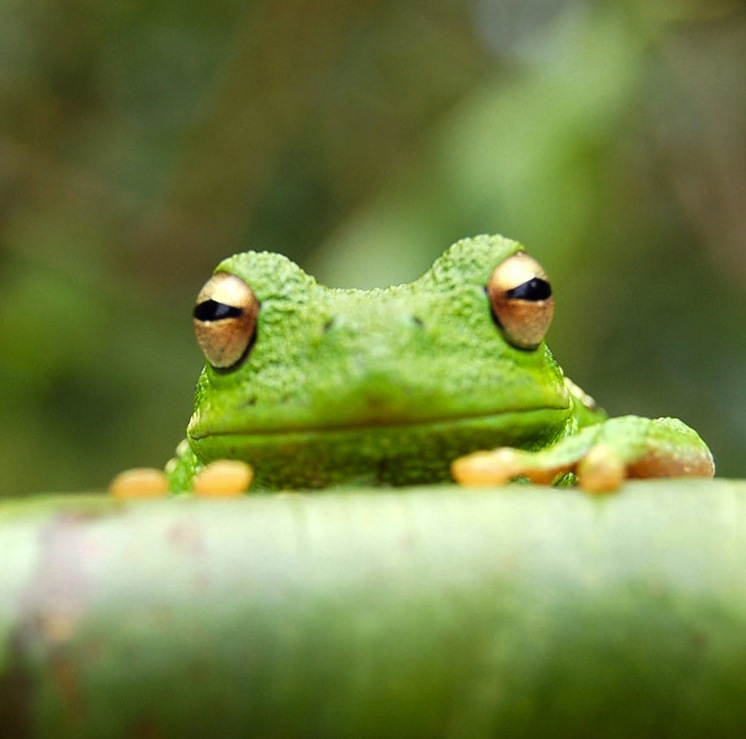
\includegraphics[width=0.125\textwidth]{frog.jpg}
\end{center}
\end{document}
